\documentclass[output=book,nonflat,modfonts,hidelinks,table]{langsci/langscibook}

\title{Metathesis and unmetathesis in Amarasi} 
\BackBody{Change your blurb in localmetadata.tex}
\dedication{For Chuck and Om Roni who laid the groundwork in analysing Amarasi.
						The giants on whose shoulders I stand.}
%\typesetter{Change typesetter in localmetadata.tex}
%\proofreader{Change proofreaders in localmetadata.tex}
\author{Owen Edwards}
% \BookDOI{}%ask coordinator for DOI
% \renewcommand{\lsISBNdigital}{000-0-000000-00-0}
% \renewcommand{\lsISBNhardcover}{000-0-000000-00-0} 
\renewcommand{\lsSeries}{sidl} % use lowercase acronym, e.g. sidl, eotms, tgdi
\renewcommand{\lsSeriesNumber}{} %will be assigned when the book enters the proofreading stage
\renewcommand{\lsID}{228}

 
 
 
 
  

%%%%%%%%%%%%%%%%%%%%%%%%%%%%%%%%
%%	Font Styles & Formatting	%%
%%%%%%%%%%%%%%%%%%%%%%%%%%%%%%%%

\newcommand{\ve}{\textit}			%vernacular	/ target language text
\newcommand{\tbr}{\textbf}		%Bold red text
\newcommand{\tcb}{\textcolor{black}}	%black colour
\renewcommand{\it}{\textit}	%italics
\newcommand{\tsc}{\textsc}	%small caps
\newcommand{\tbf}{\textbf}	%boldface

\newcommand{\sub}{\textsubscript}				%subscript
\newcommand{\su}{\textsuperscript}			%superscript
\renewcommand{\sf}[1]{\textsf{\textcolor{black}{#1}}}							%sans serif

%%%%%%%%%%%%%%%%%%%%%%%%%%%%%%%%
%%	Symbols and Characters		%%
%%%%%%%%%%%%%%%%%%%%%%%%%%%%%%%%

\newcommand{\tl}{\char`~}		%middle tilde ~
\newcommand{\x}{×} 					%times symbol ×
\newcommand{\rt}{√} 				%root symbol
\newcommand{\Q}{\textquotesingle}	%straight apostrophe
\newcommand{\<}{〈} 			%left angle (for infixes)
\renewcommand{\>}{〉} 		%right angle (for infixes)
\newcommand{\ra}{→} 		%->
\newcommand{\da}{↓} 		%downwards arrow
\newcommand{\la}{←} 		%<-
\newcommand{\lra}{↔} 		%<->
\newcommand{\0}{∅} 			%zero symbol
%\newcommand{\hand}{\raisebox{-0.3ex}{\Large ☞}} %OT pointing hand
\newcommand{\hand}{☞} 	%OT pointing hand
\renewcommand{\ast}{⁎} 	%centered asterisk
\newcommand{\gap}{\textunderscore} 	%underscore
\newcommand{\A}{α}
\newcommand{\sA}{\sub{α}}
\newcommand{\sB}{\sub{β}}
\newcommand{\br}[1]{$\overline{\textrm{#1}}$}	%Overbar (for N' etc.)

\newcommand{\vp}{\vphantom}			%space equal to height of argument
\newcommand{\hp}{\hphantom}			%space equal to width of argument
\newcommand{\lh}[1]{\leavevmode{\hp{#1}}} %space equal to width of argument for free translationa

\newcommand{\sarc}[1]{{#1}̯} %non-syllabic, combining inverted breve below i.e. u̯
\renewcommand{\j}{ʤ}				%dezh digraph
\newcommand{\tS}{ʧ}					%tesh digraph
\newcommand{\ny}{ɲ}					%palatal nasal -- enya = latin small letter n with left hook
%\newcommand{\B}{\addfontfeature{StylisticSet=20} β} %voiced bilabial fricative
\newcommand{\B}{β}	%voiced bilabial fricative
\newcommand{\tbrtb}[2]{\it{\tbf{#1}͡\tbf{#2}}} %tiebar over two boldface, italic, maroon letters -- for some reason the tiebar over a boldface character in Linux Libertine displays as  breve over the first character

%%%%%%%%%%%%%%%%%%%%%%%%%%%%%%%%%%%%%%%%%%%%%%%%%%%%
%% Tables %% Tables %% Tables %% Tables %% Tables %%
%%%%%%%%%%%%%%%%%%%%%%%%%%%%%%%%%%%%%%%%%%%%%%%%%%%%

\newcommand{\mc}{\multicolumn}									%multicolumn
\newcommand{\cgr}{\cellcolor{gray!14}}					%grey cellcolor
\newcommand{\wg}{\rowcolors{1}{white}{gray!14}} %white/grey/white alternating rowcolors
\newcommand{\gw}{\rowcolors{1}{gray!14}{white}} %grey/white/grey alternating rowcolors
\newcommand{\rcl}{\rowcolor{gray!14}}						%single grey row
\newcolumntype{g}{>{\columncolor{gray!14}}l}		%grey column
\newcommand{\stl}[1]{\setlength{\tabcolsep}{#1}}	%reduce column width in tables

%%%%%%%%%%%%%%%%%%%%%%%%%%%%%%%%
%%	Cross					References	%%
%%%%%%%%%%%%%%%%%%%%%%%%%%%%%%%%

\newcommand{\qf}[1]{(\ref{#1})}					%cross reference bracketed examples
\newcommand{\trf}[1]{Table \ref{#1}}		%cross reference Table
\newcommand{\frf}[1]{Figure \ref{#1}}		%cross reference Figure
\newcommand{\srf}[1]{\S\ref{#1}} 				%cross reference section
\newcommand{\prf}[1]{page \pageref{#1}} %cross reference page number

%\newcommand{\eax}[1]{\ea{\textnormal{#1}}}
\newcommand{\txrf}[1]{\hfill{\ttfamily\small {#1}}}			%Amarasi example information
\newcommand{\xrf}[1]{{\ttfamily\small {#1}}}						%Amarasi example information
\newcommand{\brac}[1]{\normalfont\textcolor{black}{[\sub{#1}}}  %square bracket with argument i.e. [NP
\newcommand{\bracr}[1]{\normalfont\textcolor{black}{]\sub{#1}}} %right square bracket with argument i.e. ]NP

 
\newcommand{\appref}[1]{Appendix \ref{#1}}
\newcommand{\fnref}[1]{Appendix \ref{#1}}
\newcommand{\regel}[1]{#1}
\newcommand{\vernacular}[1]{\emph{#1}}
\newcommand{\gloss}[1]{#1}

\newcounter{exx}

\usepackage{longtable}	%for multicolumn
\usepackage{multicol}	%for multicolumn
\usepackage{multirow}	%for multirow
\usepackage[linguistics]{forest}	%for syntax trees
\usepackage{cancel}	%draw X through characters
	\newcommand{\xc}{\xcancel}
\usepackage{rotating}	%rotate text (for phoneme charts)
\usepackage{amsmath}
\usepackage[shortcuts]{extdash} %to stop M-form (M\=/form breaking at the hyphen, but allowing other hyphented words to)
\usepackage{hhline}
\usepackage{subcaption}
	\captionsetup[sub]{font=small}

\usepackage{caption}						%to get captions for side-by-side tables/figures
\usepackage{varwidth}						%Center caption that includes a \newline
\DeclareCaptionFormat{CentreNewLine}{
  \begin{varwidth}{\linewidth}
    \centering
    #1#2#3%
  \end{varwidth}}
	
%%%%%%%%%%%%%%%%%%%%%%%%%%%%%%%%%%%%%%%%%%%%%%%%%%%%
%%%                                              %%%
%%%     Table notes                              %%%
%%%                                              %%%
%%%%%%%%%%%%%%%%%%%%%%%%%%%%%%%%%%%%%%%%%%%%%%%%%%%%

\usepackage{threeparttable}	%allows tables with tablenotes
	\makeatletter 
	\g@addto@macro\TPT@defaults{\footnotesize} 
	\makeatother

%%%%%%%%%%%%%%%%%%%%%%%%%%%%%%%%%%%%%%%%%%%%%%%%%%%%
%%%                                              %%%
%%%     Embedding Sound Files                    %%%
%%%                                              %%%
%%%%%%%%%%%%%%%%%%%%%%%%%%%%%%%%%%%%%%%%%%%%%%%%%%%%

\usepackage[playbutton=none,transparent=true]{media9}
	\addmediapath{relevant/audio/MP3/Ch1}		%Location of sound files
	\addmediapath{relevant/audio/MP3/Ch3}		%Location of sound files
	\addmediapath{relevant/audio/MP3/Ch4}		%Location of sound files
	\addmediapath{relevant/audio/MP3/Ch5}		%Location of sound files
	\addmediapath{relevant/audio/MP3/Ch6}		%Location of sound files
	\addmediapath{relevant/audio/MP3/Ch7}		%Location of sound files
	\addmediapath{relevant/audio/MP3/Ch8}		%Location of sound files
	\addmediapath{relevant/audio/MP3/ChA}		%Location of sound files
		\newif\ifincludeexternalmedia
%		\includeexternalmediatrue					%This line commented = Don't embed
		\includeexternalmediafalse				%This line commented = embed

\newcommand{\emb}[3]{
	\ifincludeexternalmedia
		\includemedia[addresource=#1,flashvars={source=#1 &autoPlay=true &hideBar=true}]{#2}{#3}
	\else #2 \fi}
%\newcommand{\spk}[1]{\hspace{-1mm}{$\!$}
\newcommand{\spk}[1]{{$\!$}
\begin{tikzpicture}[#1]
   \draw[thick,rounded corners=0.1pt, fill=black] (0,0.0909) -- (0,0.1636) -- (0.0909,0.1636) -- (0.1818,0.2545) -- (0.1818,0) -- (0.0909,0.0909) -- cycle;
   \draw[line width=0.65pt,line cap=round] (0.2182,0.0909) arc (-30:30:0.7273mm);
   \draw[line width=0.65pt,line cap=round] (0.2545,0.0545) arc (-30:30:1.4545mm);
   \draw[line width=0.65pt,line cap=round] (0.2909,0.0182) arc (-30:30:2.1818mm);
%\end{tikzpicture}\hspace{-1mm}} %speaker symbol
\end{tikzpicture}} %speaker symbol
\newcommand{\apl}{APlayer.swf} %to embed sound file print {\emb{<file.mp3>}{\spk{}}{\apl}}

%%%%%%%%%%%%%%%%%%%%%%%%%%%%%%%%%%%%%%%%%%%%%%%%%%%%%%%%%%%
%%%													%%%													%%%
%%%	Autosegmental Diagrams	%%%	Autosegmental Diagrams	%%%
%%% 												%%%                         %%%
%%%%%%%%%%%%%%%%%%%%%%%%%%%%%%%%%%%%%%%%%%%%%%%%%%%%%%%%%%%

\usepackage{xytree}
	\xyoption{tips}
	\newcommand{\as}{\asrnode}
	\newcommand{\exa}{\normalfont\ex\raisebox{\dimexpr-\totalheight+3.475ex\relax}}
	\newcommand{\exia}{\normalfont\raisebox{\dimexpr-\totalheight+3.475ex\relax}}
	%\newcommand{\exan}{\normalfont\ex\raisebox{\dimexpr-\totalheight+4.6825ex\relax}}
	%\newcommand{\exian}{\normalfont\raisebox{\dimexpr-\totalheight+4.6825ex\relax}}
	\newcommand{\sna}{\normalfont\sn\raisebox{\dimexpr-\totalheight+3.475ex\relax}}
%	\newcommand{\ext}{\renewcommand{\arraystretch}{1.05}}

%%%%%%%%%%%%%%%%%%%%%%%%%%%%%%%%%%%%%%%%%%%%%%%%%%%%
%%%                                              %%%
%%%           Examples                           %%%
%%%                                              %%%
%%%%%%%%%%%%%%%%%%%%%%%%%%%%%%%%%%%%%%%%%%%%%%%%%%%%

\usepackage{chngcntr}
%% to add additional information to the right of examples, uncomment the following line
%\usepackage{langsci/styles/jambox}
\usepackage{langsci/styles/langsci-optional}
%\usepackage{langsci/styles/langsci-lgr}
\usepackage{langsci/styles/langsci-glyphs}
\usepackage{langsci/styles/langsci-gb4e}
	\let\eachwordone=\itshape
	\nosinglegloss
	\judgewidth{α:}
	\counterwithin{exx}{chapter}							% reset example counter every chapter
	\renewcommand{\exp}[1]{\exi{{(\ref{#1}′)}}}	% the pre-defined gb4e \exp command has $'$ which provides a prime symbol of a different font/size.
																							% For consistency with other uses of the prime in my book (which are consistently ′ not $'$
																							% I have redefined this here.

\usepackage{pst-node}
		\newcommand{\bxA}[1]{\rnode{A}{\psframebox[linewidth=0.4pt]{#1}}}			%node-A with box
		\newcommand{\bxB}[1]{\rnode{B}{\psframebox[linewidth=0.4pt]{#1}}}			%node-B with box
		\newcommand{\bxX}[1]{\rnode{X}{\psframebox[linecolor=white,linewidth=0.4pt]{#1}}}			%node-B with box
		\newcommand{\lk}{\ncbar[arm=5pt,angle=90,linewidth=0.4pt]{->}{A}{B}}	%draw arrow between A and B
		\newcommand{\lks}{\ncbar[arm=5pt,angle=90,linewidth=0.4pt]{-}{A}{B}}	%draw arrow between A and B
		\newcommand{\gp}{\hspace{0.32em}}	%space before gloss equivalent to gap greated by \psframebox

\usepackage[english]{babel}

\usepackage{pdfpages}

%% hyphenation points for line breaks
%% Normally, automatic hyphenation in LaTeX is very good
%% If a word is mis-hyphenated, add it to this file
%%
%% add information to TeX file before \begin{document} with:
%% %% hyphenation points for line breaks
%% Normally, automatic hyphenation in LaTeX is very good
%% If a word is mis-hyphenated, add it to this file
%%
%% add information to TeX file before \begin{document} with:
%% %% hyphenation points for line breaks
%% Normally, automatic hyphenation in LaTeX is very good
%% If a word is mis-hyphenated, add it to this file
%%
%% add information to TeX file before \begin{document} with:
%% \include{localhyphenation}
\hyphenation{
affri-ca-te
affri-ca-tes
com-ple-ments
}

%\exhyphenpenalty=10000	%prevent words with hypen (i.e. `M-form' from breaking across lines)
\hyphenation{
affri-ca-te
affri-ca-tes
com-ple-ments
}

%\exhyphenpenalty=10000	%prevent words with hypen (i.e. `M-form' from breaking across lines)
\hyphenation{
affri-ca-te
affri-ca-tes
com-ple-ments
}

%\exhyphenpenalty=10000	%prevent words with hypen (i.e. `M-form' from breaking across lines)
%%%%%%%%%%%%%%%%%%%%%%%%%%%%%
%% Abbreviations & Glosses %%
%%%%%%%%%%%%%%%%%%%%%%%%%%%%%

\newcommand{\shiftleft}[2]{\makebox[0pt][r]{\makebox[#1][l]{#2}}}

\newcommand{\M}{{\textbackslash}\tsc{m}}
\newcommand{\Mv}{{\textbackslash}\tsc{m\shiftleft{0.8pt}{̿}}}
\newcommand{\Mvv}{\tsc{m\shiftleft{0.8pt}{̿}}}
\newcommand{\Mc}{{\textbackslash}\tsc{m\shiftleft{0.25pt}{\raisebox{-4pt}{\scalebox{1.75}{ͨ}}}}}
\newcommand{\MC}{M\shiftleft{1.2pt}{\raisebox{-3pt}{\scalebox{1.75}{ͨ}}}}
\newcommand{\tbrM}{{\textbackslash}\tbr{\tsc{m}}}
\newcommand{\tbrMv}{{\textbackslash}\tsc{\tbr{m}\shiftleft{1.5pt}{\textcolor{DarkRed}{̿}}}}
\newcommand{\tbrMc}{{\textbackslash}\tsc{\tbr{m}\shiftleft{0.8pt}{\raisebox{-4pt}{\scalebox{1.75}{\textcolor{DarkRed}{ͨ}}}}}}
	%\nomenclature[G]{\tsc{m}}{M-form (metathesised)}
	%\nomenclature[G]{\tsc{mͨ}}{M-form before consonant \\ cluster}
	%\nomenclature[G]{\tsc{m̿}}{M-form before vowel initial \\ enclitic}
\renewcommand{\U}{{\textbackslash}\tsc{u}}
	%\nomenclature[G]{\tsc{u}}{U-form (unmetathesised)}
	%\nomenclature[G]{\tsc{uͨ}}{U-form of consonant final stem and U-form before consonant cluster}
\newcommand{\Uc}{{\textbackslash}\tsc{u\raisebox{-4pt}{\scalebox{1.75}{ͨ}}}}
\newcommand{\Ucc}{\tsc{u\raisebox{-4pt}{\scalebox{1.75}{ͨ}}}}
\newcommand{\tbrU}{{\textbackslash}\tbr{\tsc{u}}}
\newcommand{\tbrUc}{{\textbackslash}\tsc{\tbr{u}\raisebox{-4pt}{\scalebox{1.75}{\textcolor{DarkRed}{ͨ}}}}}

%%%%%%%%%%%%%%%%%%%
%% Free Pronouns %%
%%%%%%%%%%%%%%%%%%%

\newcommand{\au}{\tsc{1sg}}					% au
	%\nomenclature[G]{1}{1\su{st} person}
	%\nomenclature[G]{\tsc{sg}}{singular}
\newcommand{\kau}{\tsc{1sg.acc}}		% kau
	%\nomenclature[G]{\tsc{acc}}{accusative}
\newcommand{\hoo}{\tsc{2sg}}						% ho
\newcommand{\koo}{\tsc{2sg.acc}}			% ko
	%\nomenclature[G]{2}{2\su{nd} person}
\newcommand{\iin}{\tsc{3sg}}					% in
	%\nomenclature[G]{3}{3\su{rd} person}
\newcommand{\eeV}{\tsc{3sg.acc}}				%	e
\newcommand{\hiit}{\tsc{1pi}}				% hit
	%\nomenclature[G]{\tsc{pi}}{plural inclusive}
\newcommand{\kiit}{\tsc{1pi.acc}}		% kit
\newcommand{\hai}{\tsc{1px}}				% hai
	%\nomenclature[G]{\tsc{px}}{plural exclusive}
\newcommand{\kai}{\tsc{1px.acc}}		% kai
\newcommand{\hii}{\tsc{2pl}}					% hi
	%\nomenclature[G]{\tsc{pl}}{plural}
\newcommand{\kii}{\tsc{2pl.acc}}			% ki
\newcommand{\siin}{\tsc{3pl}}			% sin (verbs)
\newcommand{\siinN}{\tsc{assoc.pl}}	% sin (nouns)
	%\nomenclature[G]{\tsc{assoc.pl}}{associative plural}
\newcommand{\einV}{\tsc{pl}}				% ein, =n

%%%%%%%%%%%%%%%%%%%%%%%%%%
%% Pronominal Agreement %%
%%%%%%%%%%%%%%%%%%%%%%%%%%

\renewcommand{\k}{\tsc{3pl/1gen}}			% -k
	%\nomenclature[G]{\tsc{gen}}{genitive}
\newcommand{\N}{\tsc{3sg.gen}}				% -n
\newcommand{\mg}{\tsc{1px/2gen}}			% -m
\newcommand{\f}{\tsc{0gen}}						% -f
	%\nomenclature[G]{0}{0 person}
\newcommand{\F}{\tsc{gen}}						% -f (kin)

\newcommand{\qu}{\tsc{1sg}}				% u-
\renewcommand{\mu}{\tsc{2sg}}			% mu-
\newcommand{\mut}{\tsc{2sg{\textbackslash}tr}}			% mu-
\newcommand{\na}{\tsc{3}}					% na-
\newcommand{\nat}{\tsc{3{\textbackslash}tr}}			% na- (on n- verb)
	%\nomenclature[G]{\tsc{tr}}{transitive}
\newcommand{\ta}{\tsc{1pi}}				% ta-
\newcommand{\tat}{\tsc{1pi{\textbackslash}tr}}
\newcommand{\mi}{\tsc{1px/2pl}}		% mi-
\newcommand{\q}{\tsc{1sg}}				% ʔ-
\newcommand{\m}{\tsc{1px/2}}		% m-
\newcommand{\n}{\tsc{3}}					% n-
\renewcommand{\t}{\tsc{1pi}}			% t-
\newcommand{\tg}{\tsc{0}}					% t-, ta- 0

%%%%%%%%%%%%%%%%%%%%%%%%%%%%%%%%
%% Determiners/Demonstratives %%
%%%%%%%%%%%%%%%%%%%%%%%%%%%%%%%%

\newcommand{\ii}{\tsc{1det}}				% ii
	%\nomenclature[G]{\tsc{det}}{determiner}
\newcommand{\aan}{\tsc{2det}}				% aan
\newcommand{\ee}{\tsc{3det}}				% ee
\renewcommand{\aa}{\tsc{0det}}			% aa
\newcommand{\ein}{\tsc{pl}}					% ein
\newcommand{\es}{one}								% es
\newcommand{\esc}{\tsc{cop}}				% es
	%\nomenclature[G]{\tsc{cop}}{copula}
\newcommand{\oo}{\tsc{refl}}				% o-n
	%\nomenclature[G]{\tsc{refl}}{reflexive}

\renewcommand{\ia}{\tsc{1dem}}				% ia
	%\nomenclature[G]{\tsc{dem}}{demonstrative}
\newcommand{\naan}{\tsc{2dem}}			% naan
\newcommand{\nee}{\tsc{3dem}}				% nee
\newcommand{\naa}{\tsc{0dem}}				% naa

%%%%%%%%%%%%%%%%%%%%
%% Prepositionals %%
%%%%%%%%%%%%%%%%%%%%

\newcommand{\bi}{\tsc{rl.loc}}			% n-bi
\newcommand{\biqaka}{\tsc{rl.loc}}			% n-bi'aka (Ro'is)
	%\nomenclature[G]{\tsc{loc}}{locative}
	%\nomenclature[G]{\tsc{rl}}{realis}
\newcommand{\et}{\tsc{ipfv.loc}}				% et, es
\newcommand{\ek}{\tsc{loc}}				% ek (Ro'is)
	%\nomenclature[G]{\tsc{ipfv}}{imperfective}
\newcommand{\on}{\tsc{irr.loc}}		% on
\newcommand{\eu}{\tsc{dat}}				% n-eu
	%\nomenclature[G]{\tsc{dat}}{dative}
\newcommand{\ok}{with}						% n-ok
\newcommand{\qko}{\tsc{abl}}			% na-ʔko
	%\nomenclature[G]{\tsc{abl}}{ablative}

%%%%%%%%%%%%%%%%%%%
%% Other Affixes %%
%%%%%%%%%%%%%%%%%%%

\renewcommand{\a}{\hphantom{a|}}			% a-
\newcommand{\mv}{\tsc{stat}}			% m-
	%\nomenclature[G]{\tsc{stat}}{stative}
\renewcommand{\b}{\tsc{tr}}			% -b
\newcommand{\qU}{\tsc{u}}				% -ʔ
\newcommand{\qnum}{\tsc{ord}}				% -ʔ
	%\nomenclature[G]{\tsc{ord}}{ordinal}
\newcommand{\mak}{\tsc{recp}}		% ma-
	%\nomenclature[G]{\tsc{recp}}{reciprocal}
\newcommand{\ma}{\tsc{prop}}		% ma-
	%\nomenclature[G]{\tsc{prop}}{property}
\newcommand{\at}{\tsc{nml}}		% a-...-t
	%\nomenclature[G]{\tsc{nml}}{nominaliser}
\newcommand{\qq}{\tsc{nml}}		% ʔ-...-ʔ
\newcommand{\qV}{\tsc{tr}}		% ʔ-...-ʔ
\newcommand{\prd}{\tsc{intns}{\tl}}		% CVC-
	%\nomenclature[G]{\tsc{intns}}{intensive}
\newcommand{\frd}{\tsc{frd}{\tl}}		% frd-
	%\nomenclature[G]{\tsc{frd}}{full reduplication}
	
%%%%%%%%%%%%%%%%%%%%
%% Other Functors %%
%%%%%%%%%%%%%%%%%%%%

\newcommand{\maeq}{\tsc{neg}}				% ka=
\newcommand{\ka}{\tsc{neg}}				% ka=
	%\nomenclature[G]{\tsc{neg}}{negative}
\newcommand{\fa}{\tsc{neg}}				% =fa, =f
\newcommand{\te}{\tsc{sub}}				% =te
	%\nomenclature[G]{\tsc{sub}}{subordinate}
\newcommand{\een}{\tsc{incep}}			% =een
	%\nomenclature[G]{\tsc{incep}}{inceptive}
\newcommand{\BI}{Ms.}							% bi
\newcommand{\naiq}{Mr.}						% naiʔ
\newcommand{\he}{\tsc{irr}}				% he
	%\nomenclature[G]{\tsc{irr}}{irrealis}
\newcommand{\ak}{\tsc{quot}}
	%\nomenclature[G]{\tsc{quot}}{quotative}
\newcommand{\nai}{\tsc{imp}}
	%\nomenclature[G]{\tsc{imp}}{impertive}
\newcommand{\req}{\tsc{rel}}			% reʔ
	%\nomenclature[G]{\tsc{rel}}{relativiser}
\newcommand{\reqt}{\tsc{top}}			% reʔ
	%\nomenclature[G]{\tsc{top}}{topic}
\newcommand{\kaah}{\tsc{neg}}			% kah
\newcommand{\kais}{\tsc{proh}}		% kais(aʔ)
	%\nomenclature[G]{\tsc{proh}}{prohibitive}
\newcommand{\manaq}{\tsc{count}}		% kais(aʔ)
	%\nomenclature[G]{\tsc{count}}{counter}

%%%%%%%%%%%%%%%%%
%% Other Words %%
%%%%%%%%%%%%%%%%%

\newcommand{\ana}{\tsc{res}}				% ana
	%\nomenclature[G]{\tsc{res}}{resultative}
\newcommand{\uma}{1/{\mu}{\textbackslash}come}	% uma
\newcommand{\ima}{{\mi}{\textbackslash}come}				% ima
\newcommand{\nema}{{\n}{\textbackslash}come}				% nema

\newcommand{\tua}{\tsc{addr}}					% tua
	%\nomenclature[G]{\tsc{addr}}{addressee}
\newcommand{\aaQ}{\tsc{q}}						% aa?
	%\nomenclature[G]{\tsc{q}}{question}
\newcommand{\nehh}{\tsc{pause}}						% aa?

%%%%%%%%%%%%%%%%%%%%
%% Other %%	Other %%
%%%%%%%%%%%%%%%%%%%%

%\nomenclature[K]{PF}{grandfather}
%\nomenclature[K]{PM}{grandmother}
%\nomenclature[K]{F}{father}
%\nomenclature[K]{M}{mother}
%\nomenclature[K]{MB/FZ}{parent's opposite sex sibling}
%\nomenclature[K]{eSi}{same sex elder sibling}
%\nomenclature[K]{ySi}{same sex younger sibling}
%\nomenclature[K]{fB}{woman's brother}
%\nomenclature[K]{mZ}{man's sister}
%\nomenclature[K]{DH}{daughter's husband}
%\nomenclature[K]{SW}{son's wife}
%\nomenclature[K]{WB/ZH}{same sex sibling of spouse, opposite sex sibling's spouse}
%\nomenclature[K]{CC}{grandchild}
%\nomenclature[K]{CCC}{great-grandchild}
%\nomenclature[K]{PPP}{forefather}
%\nomenclature[K]{PMP}{Proto-Malayo-Polynesian}
	% Glosses and Abbreviations
\bibliography{relevant/localbibliography}
\graphicspath{{relevant/figures/}}

%\includeonly{chapters/Conclusion/ConCon}
\usepackage{chngcntr}
\begin{document}

\maketitle
\frontmatter

\currentpdfbookmark{Contents}{name} % adds a PDF bookmark
\tableofcontents
	\addchap{Preface}
\begin{refsection}

This book is a revised version of my PhD Thesis,
submitted August 2016 awarded July 2017.
The analyses in this work remain broadly the same as those in my PhD thesis,
but several areas have undergone substantial revision.

The most significant analytical revision
is in the analysis of phonologically conditioned
metathesis (Chapter \ref{ch:PhoMet}).
This revision is informed by a proper analysis of
the prosodic structures of Amarasi including
the Prosodic Word (\srf{sec:ProsStr}).
A proper understanding and description
of Amarasi prosodic structures was mostly lacking in the earlier work.

Structurally, chapter \ref{ch:SynchMet}
has been significantly reorganised on the basis
of comments from the reviewers in order to clarify
the distinction between the three types of metathesis
I identify, as well as to avoid shoe-horning languages
with multiple kinds of metathesis into a single category.

Since the submission of my PhD thesis much more data
on other varieties of Meto has also become available.
In addition to including such data where it is relevant,
it has also informed my analysis of Amarasi in several important respects.
Thus, for instance, vowel initial enclitics which were mostly represented
as monosyllables in my earlier work are now properly
represented as containing two vowels (\srf{sec:HisDev}).

Of particular prominence is the additional data
on Ro{\Q}is Amarasi (the other major dialect of Amarasi)
for which I only had limited preliminary data for my PhD thesis.
I have included several sections discussing
the Ro{\Q}is data as it has several important
differences to that of Kotos Amarasi
(e.g. \srf{sec:RoqAnaCCIniMod}, \srf{sec:DisDriMetRoqAma}).

I have also included a more proper discussion
of alternate analyses of the structure of Amarasi
metathesis (\srf{sec:AltApp}), as well
as syntactic metathesis (\srf{sec:ProsMet}).

Finally, numerous errors have been corrected.
These include typographical errors
and minor errors in the actual data.

%\printbibliography[heading=subbibliography]
\end{refsection}


	\addchap{Acknowledgements}
\begin{refsection}

Given that this work is a revision of my PhD thesis,
I must also revise my acknowledgements.
No names need be subtracted from the acknowledgements for my PhD thesis,
but several must be added or re-emphasised.

First and foremost, and again, I would like to thank
\tbf{Heronimus Bani} and \tbf{Charles Grimes}.
My PhD work would have been a complete disaster without
the groundwork laid by Roni and Chuck and
subsequently this book would never have appeared.
I look forward to continuing to to work with them in championing,
in whatever small way I can, the languages and peoples of Timor.

Selain itu beta ju mau minta terima kasih buat semua
orang Tunbaun dong dengan orang Buraen dong.
Khususunya \tbf{Om Melo} dengan dia pung keluarga,
dan \tbf{bapa Toni} dengan \tbf{mama Ketsia};
orang dong yang mengajar beta logat Ro{\Q}is.

Secondly, I would like to thank the examiners of my thesis:
\tbf{Anthony Jukes}, \tbf{Daniel Kaufmann} and \tbf{Marian Klamer}.
Their perceptive comments on the submitted version of this thesis
led to many useful revisions of that work, some of which have
taken until now to be fully implemented.

In particular, Daniel Kaufmann suggested
the revised prosodic structure of hosts and enclitics which
has made my analysis of phonological metathesis much clearer
and more typologically plausible.

Marian Klamer provided me with the job during
which I have had the freedom to produce this work.
It is with gratitude that I say here that
revision of my thesis for publication was supported
by the VICI research project ``Reconstructing the past
through languages of the present: the Lesser Sunda Islands''
funded by the Netherlands Organisation for Scientific
Research, project number 277-70-012.

Thirdly, I would like to thank the anonymous reviewers
who read the submitted version of this book.
While it is often frustrating dealing with comments from reviewers,
in my experience, they are nearly always on point and 
addressing them properly yields a better result.
I hope these reviewers feel I have honoured the time
they put into assessing this work by properly
considering their insightful criticisms.

Fourthly, I would like to thank the editors of Language
Science Press, \tbf{Martin Haspelmath} and \tbf{Sebastian Nordhoff}
who have guided the manuscript to publication,
as well as the proofreaders who caught many of the
typographical errors and style issues.
Listed in reverse-alphabetical order:
\tbf{Jeroen van de Weijer}, \tbf{Brett Reynolds},
\tbf{Ludger Paschen}, \tbf{Sebastian Nordhoff}, \tbf{Steven Kaye},
\tbf{Christian Döhler}, \tbf{Tom Bossuyt},
\tbf{Laura Arnold}, \tbf{Cormac Anderson},
and \tbf{Sauvane Agnès}.
I would also like to thank \tbf{Philipp Conzett}
and TROLLing (The Tromsø Repository of Language and Linguistics) 
where the recordings on which this book is based are hosted.

The deficiencies which undoubtedly remain in this
work are entirely my own responsibility
and none of the people mentioned in
these acknowledgements are responsible for them.

Finally, from the moment I submitted my PhD thesis
I have had the pleasure of getting to know \tbf{Kirsten Culhane}.
I have enjoyed spending time with her and conversations
with her have contributed to many different parts of this work.
\it{Bi Kirsten, au {\Q}neek ko msa{\Q}.}

\vspace{\baselineskip}

\noindent
\it{Behold, I will create new heavens and a new earth.
The former things will not be remembered,
nor will they come to mind.}
\hfill(Isaiah 65:17a)

\vspace{\baselineskip}

\noindent
\it{Rarit In re{\Q} antuun On anbi {\Q}toko prenat naan, na{\Q}uab am nak,
``Amkius mirek-reko{\Q}, natuin Au u{\Q}fe{\Q}u are{\Q} kanan saa{\Q}-saa{\Q}.''}
\hfill{(Rasi Mnitas neu nai{\Q} Yohanis 21.5a)}

%\printbibliography[heading=subbibliography]
\end{refsection}


	\addchap{Abbreviations and symbols}\label{ch:Abb}

% \addchap{Abbreviations and symbols}

\begin{multicols}{2} 


%en-dash
%hyphen
%underscore
%vertical bar

%\begin{tabular}{lp{4.5cm}} 
\begin{tabular}{lp{7.5cm}} 
	\mc{2}{l}{see \srf{sec:PreDat} for full notational conventions} \\
	-- & {false start (en-dash)} \\
	%- & affix \\ %Leipzig
	%{\tl} & reduplication \\ %Leipzig
	{\gap} & {non-compositional phrase (underscore)} \\
	| & {epenthesis (vertical bar)} \\
	{0}	&	{0 person}		\\	
%	{1}	&	{1\su{st} person}		\\	%Leipzig
%	{2}	&	{2\su{nd} person}		\\	%Leipzig
%	{3}	&	{3\su{rd} person}		\\	%Leipzig
%	{\tsc{abl}}	&	{ablative}		\\	%Leipzig
%	{\tsc{acc}}	&	{accusative}		\\	%Leipzig
	{\tsc{addr}}	&	{addressee}		\\	
	{\tsc{assoc.pl}}	&	{associative plural}		\\	
	{CC}	&	{grandchild}		\\	
%%	{CCC}	&	{great-grandchild}		\\	
%	{\tsc{cop}}	&	{copula}		\\	%Leipzig
	{\tsc{count}}	&	{counter}		\\	
%	{\tsc{dat}}	&	{dative}		\\	%Leipzig
%	{\tsc{dem}}	&	{demonstrative}		\\	%Leipzig
%	{\tsc{det}}	&	{determiner}		\\	%Leipzig
%%	{DH}	&	{daughter's husband}		\\	
	{eSi}	&	{elder sibling}		\\	
%%	{F}	&	{father}		\\	
%%	{fB}	&	{woman's brother}		\\	
	{\tsc{frd}}	&	{full reduplication}		\\	
%	{\tsc{gen}}	&	{genitive}		\\	%Leipzig
%	{\tsc{imp}}	&	{impertive}		\\	%Leipzig
	{\tsc{incep}}	&	{inceptive}		\\	
	{\tsc{intns}}	&	{intensive}		\\	
%	{\tsc{ipfv}}	&	{imperfective}		\\	%Leipzig
%	{\tsc{irr}}	&	{irrealis}		\\	%Leipzig
%	{\tsc{loc}}	&	{locative}		\\	%Leipzig
%%	{M}	&	{mother}		\\	
	{\tsc{m}}	&	{M-form (metathesised)}		\\	
	{\tsc{m\shiftleft{0.25pt}{\raisebox{-4pt}{\scalebox{1.75}{ͨ}}}}}	&	{M-form before consonant cluster (\srf{sec:CCIniMod})}		\\	
	{\Mvv}	&	{M-form before vowel initial enclitic (chapter \ref{ch:PhoMet})}		\\	
	{MB/FZ}	&	{parent's opposite sex sibling}		\\	
	{mZ}	&	{man's sister}		\\	
%	{\tsc{neg}}	&	{negative}		\\	%Leipzig
	{\tsc{nml}}	&	{nominaliser}		\\	
%	{\tsc{ord}}	&	{ordinal}		\\	%Leipzig
	{PF}	&	{grandfather}		\\	
	{\tsc{pi}}	&	{plural inclusive}		\\	
%	{\tsc{pl}}	&	{plural}		\\	%Leipzig
	{PM}	&	{grandmother}		\\	
	{PMP}	&	{Proto-Malayo-Polynesian}		\\	
%%	{PPP}	&	{ancestor}		\\	
%	{\tsc{proh}}	&	{prohibitive}		\\	%Leipzig	
	{\tsc{prop}}	&	{property}		\\
	{\tsc{px}}	&	{plural exclusive}		\\	
%	{\tsc{q}}	&	{question}		\\	%Leipzig
%	{\tsc{quot}}	&	{quotative}		\\	%Leipzig
%	{\tsc{recp}}	&	{reciprocal}		\\	%Leipzig
%	{\tsc{refl}}	&	{reflexive}		\\	%Leipzig
%	{\tsc{rel}}	&	{relativiser}		\\	%Leipzig
%	{\tsc{res}}	&	{resultative}		\\	%Leipzig
	{\tsc{rl}}	&	{realis}		\\	
%	{\tsc{sg}}	&	{singular}		\\	%Leipzig
%	{\tsc{stat}}	&	{stative}		\\	%Leipzig
%	{\tsc{sub}}	&	{subordinate}		\\	%Leipzig
%%	{SW}	&	{son's wife}		\\	
	{\tsc{top}}	&	{topic}		\\	
	{\tsc{tr}}	&	{transitive}		\\	
	{\tsc{u}}	&	{U-form (unmetathesised)}		\\	
	{\Ucc}	&	{U-form of consonant final stem (\srf{sec:ConFinVer}) and} \\
					& {U-form before consonant cluster (\srf{sec:VerBefCC})}		\\	
%%	{WB/ZH}	&	{same sex sibling of spouse, opposite sex sibling's spouse}		\\	
	{ySi}	&	{younger sibling}		\\
\end{tabular}
 
\end{multicols} 
\mainmatter

\chapter{Introduction}

\section{Overview}
This book is about synchronic metathesis.
One well known case of synchronic metathesis comes
from Rotuman, in which many words have two forms,
such as \it{pu\tbr{re}} {\tl} \it{pu\tbr{er}} `rule, decide'
(\citealp[14]{ch40}, discussed in more detail in \srf{sec:Rot}).
In this book I present new data from Amarasi,
a language which also has synchronic metathesis.
Observe the natural textual data in \qf{ex:130902-1, 1.43 ch:Intr} below.

\begin{exe}
	\ex{Going to a party: \txrf{130902-1, 1.43}{\emb{130902-1-01-43.mp3}{\spk{}}{\apl}}}\label{ex:130902-1, 1.43 ch:Intr}
	\begin{xlist}
		\ex{\gll	oras hai m-nao =te, \\
							time {\hai} {\m}-go ={\te}\\
				\glt	`While we were going,' \txrf{}}
		\ex{\gll	naiʔ Owen ina ʔpiurʔ=ee n-mo\tbr{uf}, n-mo\tbr{fu} =ma na-mneuk.\\
							{\naiq} Owen {\iin} cloth={\ee} {\n}-fall {\n}-fall =and {\na}-lose\\
				\glt	`Owen's handkerchief fell, it fell and was lost.'}
	\end{xlist}
\end{exe}

The metathesis of Amarasi \ve{mofu} {\tl} \ve{mouf} `fall'
in \qf{ex:130902-1, 1.43 ch:Intr} is formally almost identical to Rotuman
metathesis in examples such as \it{pure} {\tl} \it{puer} `rule, decide'.
In each case the final CV sequence of a CVCV stem metathesises to VC,
as illustrated in \qf{as:Metathesis} below with
the architecture of Autosegmental Phonology \citep{go76}.

\begin{multicols}{3}
	\begin{exe}
		\ex{\begin{xlist}
			\exa{\xy
				<0em,2.5cm>*\as{\x}="x1",<1em,2.5cm>*\as{\x}="x2",<2em,2.5cm>*\as{\x}="x3",<3em,2.5cm>*\as{\x}="x4",,
				<0em,1.5cm>*\as{\hp{\sub{1}}C\sub{1}}="C1",<1em,1.5cm>*\as{\hp{\sub{2}}V\sub{2}}="V1",
				<2em,1.5cm>*\as{\hp{\sub{3}}C\sub{3}}="C2",<3em,1.5cm>*\as{\hp{\sub{4}}V\sub{4}}="V2",
				<0em,0.5cm>*\as{p}="c1",<1em,0.5cm>*\as{u}="v1",<2em,0.5cm>*\as{r}="c2",<3em,0.5cm>*\as{e}="v2",
				<0em,0cm>*\as{m}="c1a",<1em,0cm>*\as{o}="v1a",<2em,0cm>*\as{f}="c2a",<3em,0cm>*\as{u}="v2a",
				"C1"+U;"x1"+D**\dir{-};"V1"+U;"x2"+D**\dir{-};"C2"+U;"x3"+D**\dir{-};"V2"+U;"x4"+D**\dir{-};
				"c1"+U;"C1"+D**\dir{-};"v1"+U;"V1"+D**\dir{-};"c2"+U;"C2"+D**\dir{-};"v2"+U;"V2"+D**\dir{-};
			\endxy}
			\exa{\xy
				<0em,2.5cm>*\as{\x}="x1",<1em,2.5cm>*\as{\x}="x2",<2em,2.5cm>*\as{\x}="x3",<3em,2.5cm>*\as{\x}="x4",,
				<0em,1.5cm>*\as{\hp{\sub{1}}C\sub{1}}="C1",<1em,1.5cm>*\as{\hp{\sub{2}}V\sub{2}}="V1",
				<2em,1.5cm>*\as{\hp{\sub{3}}C\sub{3}}="C2",<3em,1.5cm>*\as{\hp{\sub{4}}V\sub{4}}="V2",
				<0em,0.5cm>*\as{p}="c1",<1em,0.5cm>*\as{u}="v1",<2em,0.5cm>*\as{r}="c2",<3em,0.5cm>*\as{e}="v2",
				<0em,0cm>*\as{m}="c1a",<1em,0cm>*\as{o}="v1a",<2em,0cm>*\as{f}="c2a",<3em,0cm>*\as{u}="v2a",
				"C1"+U;"x1"+D**\dir{-};"V1"+U;"x2"+D**\dir{-};"C2"+U;"x4"+D**\dir{.};"V2"+U;"x3"+D**\dir{.};
				"c1"+U;"C1"+D**\dir{-};"v1"+U;"V1"+D**\dir{-};"c2"+U;"C2"+D**\dir{-};"v2"+U;"V2"+D**\dir{-};
			\endxy}
			\exa{\xy
				<0em,2.5cm>*\as{\x}="x1",<1em,2.5cm>*\as{\x}="x2",<2em,2.5cm>*\as{\x}="x3",<3em,2.5cm>*\as{\x}="x4",,
				<0em,1.5cm>*\as{\hp{\sub{1}}C\sub{1}}="C1",<1em,1.5cm>*\as{\hp{\sub{2}}V\sub{2}}="V1",
				<2em,1.5cm>*\as{\hp{\sub{4}}V\sub{4}}="C2",<3em,1.5cm>*\as{\hp{\sub{3}}C\sub{3}}="V2",
				<0em,0.5cm>*\as{p}="c1",<1em,0.5cm>*\as{u}="v1",<2em,0.5cm>*\as{e}="c2",<3em,0.5cm>*\as{r}="v2",
				<0em,0cm>*\as{m}="c1a",<1em,0cm>*\as{o}="v1a",<2em,0cm>*\as{u}="c2a",<3em,0cm>*\as{f}="v2a",
				"C1"+U;"x1"+D**\dir{-};"V1"+U;"x2"+D**\dir{-};"C2"+U;"x3"+D**\dir{-};"V2"+U;"x4"+D**\dir{-};
				"c1"+U;"C1"+D**\dir{-};"v1"+U;"V1"+D**\dir{-};"c2"+U;"C2"+D**\dir{-};"v2"+U;"V2"+D**\dir{-};
			\endxy}		
		\end{xlist}}\label{as:Metathesis}
	\end{exe}
\end{multicols}

Synchronic metathesis in Amarasi is phonologically very similar
to previously described cases in other languages.
Furthermore, in certain environments the phonology alone
determines whether the metathesised or unmetathesised
form of a word will appear in Amarasi.
However, phonology alone cannot predict that reversal of the position of the
metathesised and unmetathesised words in \qf{ex:130902-1, 1.43 ch:Intr}
produces a sentence judged ungrammatical by native speakers,
as shown in \qf{ex:el. 22/02/16 p.19}.

\begin{exe}
	\ex[*]{\gll	naiʔ Owen ina ʔpiurʔ=ee n-mo\tbr{fu}, n-mo\tbr{uf} =ma na-mneuk.\\
						{\naiq} Owen {\iin} cloth={\ee} {\n}-fall {\n}-fall =and {\na}-lose\\
			\glt	`(Owen's handkerchief fell, it fell and was lost.)' \txrf{elicit. 22/02/16 p.19}
			}\label{ex:el. 22/02/16 p.19}
\end{exe}

The forms of synchronic metathesis in several languages have been well described.
This has lead to much useful discussion about the kinds
of phonological models which best handle metathesis,
as found in works including
\cite{be87,huen95,hu98,huse04,hu04}, and \cite{he04}, among others.

Despite this interest in the form of synchronic metathesis,
there has been relatively little attention given to
the functions of synchronic metathesis
and the different environments in which an unmetathesised
or metathesised form of a word is used.
This work partially redresses this imbalance.
I provide a detailed analysis of the functions and
environments of synchronic metathesis in Amarasi.
This includes one instance of phonologically conditioned metathesis
and two different morphological uses of metathesis,
neither of which can be reduced to a phonologically conditioned process.

I begin in Chapter \ref{ch:SynchMet} with a discussion
of processes of synchronic metathesis in languages of the world.
The focus in this chapter is on languages spoken in the same region
as Amarasi, particularly languages with morphological metathesis.
There are many similarities in both the form and use of metathesis in these languages.
Chapter \ref{ch:SynchMet} allows me to position the Amarasi
data within its geographic and typological context.

After a discussion of Amarasi phonology and phonotactics
in Chapter \ref{ch:AmaPho}, in Chapter \ref{ch:StrMetAma}
I provide a detailed investigation of the form of metathesis in Amarasi.
Depending on the phonotactic structure of the stem to which it applies,
metathesis is associated with a bewildering
array of disparate phonological processes including
vowel deletion, consonant deletion, consonant insertion,
and multiple kinds of vowel assimilation.
All these phonological processes
can be derived from a single process of metathesis and
one associated morphemically conditioned process
by proposing that Amarasi has an obligatory
CVCVC foot in which C-slots can be empty.

The structure of the words \ve{fatu} `stone', \ve{kaut} `papaya' and \ve{ai} `fire'
under this analysis are given in \qf{as:fatu/kaut/ai ch:Int} below.
Evidence independent of metathesis for empty C-slots in Amarasi 
is presented in (\srf{sec:EmpCSlo}).
Such evidence consists of five language-internal
phenomena as well as comparative data.

\begin{multicols}{3}
	\begin{exe}
		\ex{\begin{xlist}
			\exa{\xy
				<0cm,1cm>*\as{C}="C1",<1em,1cm>*\as{V}="V1",<2em,1cm>*\as{C}="C2",<3em,1cm>*\as{V}="V2",<4em,1cm>*\as{C}="C3",
				<0em,0cm>*\as{f}="c1",<1em,0cm>*\as{a}="v1",<2em,0cm>*\as{t}="c2",<3em,0cm>*\as{u}="v2",
				"c1"+U;"C1"+D**\dir{-};"c2"+U;"C2"+D**\dir{-};"v1"+U;"V1"+D**\dir{-};"v2"+U;"V2"+D**\dir{-};
			\endxy}
			\exa{\xy
				<0em,1cm>*\as{C}="C1",<1em,1cm>*\as{V}="V1",<2em,1cm>*\as{C}="C2",<3em,1cm>*\as{V}="V2",<4em,1cm>*\as{C}="C3",
				<0em,0cm>*\as{k}="c1",<1em,0cm>*\as{a}="v1",<3em,0cm>*\as{u}="v2",<4em,0cm>*\as{t}="c3",
				"c1"+U;"C1"+D**\dir{-};"c3"+U;"C3"+D**\dir{-};"v1"+U;"V1"+D**\dir{-};"v2"+U;"V2"+D**\dir{-};
			\endxy}
			\exa{\xy
				<0em,1cm>*\as{C}="C1",<1em,1cm>*\as{V}="V1",<2em,1cm>*\as{C}="C2",<3em,1cm>*\as{V}="V2",<4em,1cm>*\as{C}="C3",
				<1em,0cm>*\as{a}="v1",<3em,0cm>*\as{i}="v2",
				"v1"+U;"V1"+D**\dir{-};"v2"+U;"V2"+D**\dir{-};
			\endxy}
		\end{xlist}}\label{as:fatu/kaut/ai ch:Int}
	\end{exe}
\end{multicols}

The presence of phonological processes in addition to metathesis
leads me to label forms corresponding to unmetathesised forms as \emph{U\=/forms}
and those corresponding to metathesised forms as \emph{M\=/forms}.\footnote{
		The terms U\=/form and M\=/form can be taken as abbreviations for the form
		where \emph{U} stands for \emph{unmetathesised} and \emph{M} for \emph{metathesised}.
		They can also be taken as abbreviations for the functions of these forms,
		as in the syntax M\=/forms mark \emph{\tbf{m}odification}
		and in the discourse U\=/forms mark \emph{\tbf{u}nresolved} events or situations.
		The \emph{U} in U\=/form can also be an abbreviation for
		the morphologically \emph{\tbf{u}nderlying} form.}

In Chapter \ref{ch:PhoMet} I analyse phonologically conditioned metathesis in Amarasi.
Before vowel-initial enclitics, metathesis occurs
to clearly mark a phonological boundary between
a clitic host and vowel-initial enclitic.
The final consonant of a clitic host is shared between the host and clitic.
Metathesis creates a final consonant cluster which is resolved
by the final consonant de-linking from the clitic host but remaining linked to the enclitic,
thus creating a crisp edge between the host and enclitic.

In chapters \ref{ch:SynMet} and \ref{ch:DisMet}
I provide detailed analyses of morphological metathesis in Amarasi.
Amarasi has two morphological uses of metathesis:
one taken by medial members of phrases (noun phrases or verb phrases)
to mark the internal syntactic structure of the phrase
and one taken by final members of phrases
which marks discourse structures.
These two morphological uses of metathesis
occur in complementary environments:
phrase medial and phrase final.
As a result there is no competition
between each morphological use of metathesis
and no direct structural interaction between them.
A single sentence may contain both types of morphological
metathesis with the medial members of a particular
phrase expressing the internal syntax of this phrase
and the final member using metathesis to 
mark the discourse status of the phrase.

In Chapter \ref{ch:SynMet} I provide a detailed analysis of Amarasi metathesis within the syntax.
In the syntax metathesis is a morphological process
taken by medial members of a phrase to signal attributive modification.
Metathesis is a construct form which marks the presence of a dependent
modifier of the same word class as the head, as illustrated in \qf{ex:Fatu+Koqu2} below.
Metathesis alone distinguishes attributive phrases from
phrases with a different syntactic structure, such as equative clauses,
illustrated in \qf{ex:Fatu+Koqu1} below.
Within the syntax a metathesised form cannot occur at the end of a phrase
and thus usually entails the presence of an unmetathesised form which syntactically completes it.
Metathesised and unmetathesised forms comprise a parallel
and complementary pair of morphological forms within the syntax.

\begin{multicols}{2}
	\begin{exe}
		\ex{
			\begin{xlist}
				\ex{\gll \brac{NP} fa\tbr{ut} koʔu \bracr{}\\
								%	\hp{\brac{NP}} fatu koʔu {}\\
									{} stone big {}\\
						\glt \lh{\brac{NP} }`(a) big stone'}\label{ex:Fatu+Koqu2}
				\ex{\gll \brac{NP} fa\tbr{tu} \bracr{} \brac{NP} koʔu \bracr{}\\
								%	\hp{\brac{NP}} fatu {} {} koʔu {}\\
									{} stone {} {} big {}\\
						\glt \lh{\brac{NP} }`Stones are big.'}\label{ex:Fatu+Koqu1}
			\end{xlist}
		}\label{ex:Fatu+Koqu}
	\end{exe}
\end{multicols}

In Chapter \ref{ch:DisMet} I provide a detailed analysis of Amarasi metathesis within the discourse.
In the discourse an unmetathesised phrase-final form marks an unresolved event or situation
which requires another phrase or clause to achieve resolution.
This is the use of metathesis illustrated in \qf{ex:130902-1, 1.43 ch:Intr} above.
A discourse-driven unmetathesised form cannot occur in isolation
and typically requires a metathesised form to achieve resolution.
Unmetathesised and metathesised forms comprise a complementary and
parallel pair of morphological forms within the discourse.

I conclude in Chapter \ref{ch:ConCon} with a unified analysis Amarasi metathesis.
Metathesis in Amarasi is not merely a phonological epiphenomenon or exotic curiosity.
Rather, metathesis is the key which unlocks the structure and genius of the Amarasi language.
Metathesis also reflects fundamental Timorese notions of societal and cosmic organisation.
Metathesis is one marker of identity in a region obsessed with marking multiple
levels of identity between different groups.

The complementarity of metathesis and unmetathesis within the syntax and that within discourse
-- and also cross-cutting discourse and syntax --
reflects the Timorese division of the world into a series of parallel and complementary pairs.
More than simply being the key which unlocks the structure of the language,
metathesis is a deep reflection of the structure of Amarasi society and culture.

This book also contains four appendices.
Appendix \ref{ch:MorphSketch} provides a sketch of affixal morphology in Amarasi.
Appendix \ref{app:MorMet} discusses cases of morphological metathesis
in languages outside of the greater Timor region.
Appendix \ref{app:SelAmaTex} provides four complete
glossed Amarasi texts of different genres:
one historical narrative, one myth, one conversation
and one Ro{\Q}is Amarasi narrative.
These three texts allow the reader to see
how metathesis operates across a complete text.
Appendix D
% \ref{app:TexInd}
provides information and metadata
on the texts referred to throughout this book,
as discussed further in \srf{sec:PreDat} below.

\section{Language background}\label{sec:LanBac}
Amarasi is a variety of Meto.
Meto, also known as Uab Meto, Dawan(ese), Timorese or Atoni,\footnote{
		In earlier works I referred to this language cluster as Uab Meto.
		In Amarasi \ve{uab metoʔ} can be glossed as `dry/indigenous speech'.
		However, not all Meto speaking areas use \ve{uab} for `speech'.
		Thus, in Amfo{\Q}an `speech' is \ve{aguab} while
		in some other areas, such as Timaus, it is \ve{molok}.
		Use of \emph{Meto} alone as the name of the language cluster
		thus covers more varieties in an emic manner.
		It also matches native use in which \ve{metoʔ} alone
		can refer to the language.
		Such use is seen in phrases such as
		\ve{iin nahiin metoʔ} `S/he knows (how to speak) Meto'.}
is a cluster of closely related Austronesian languages
and dialects spoken on the western part of the island of Timor;
both in the East Timorese enclave of Oecusse,
as well as in the Indonesian province of Nusa Tenggara Timur.
The location of the Meto cluster is shown in \frf{fig:LanGroTim}
along with other languages of Timor.
The identity and location of languages in Timor-Leste
in \frf{fig:LanGroTim} is mainly based on \cite{wiklwi15}.

\begin{figure}[h]
	\caption{Language groups of Timor}\label{fig:LanGroTim}
	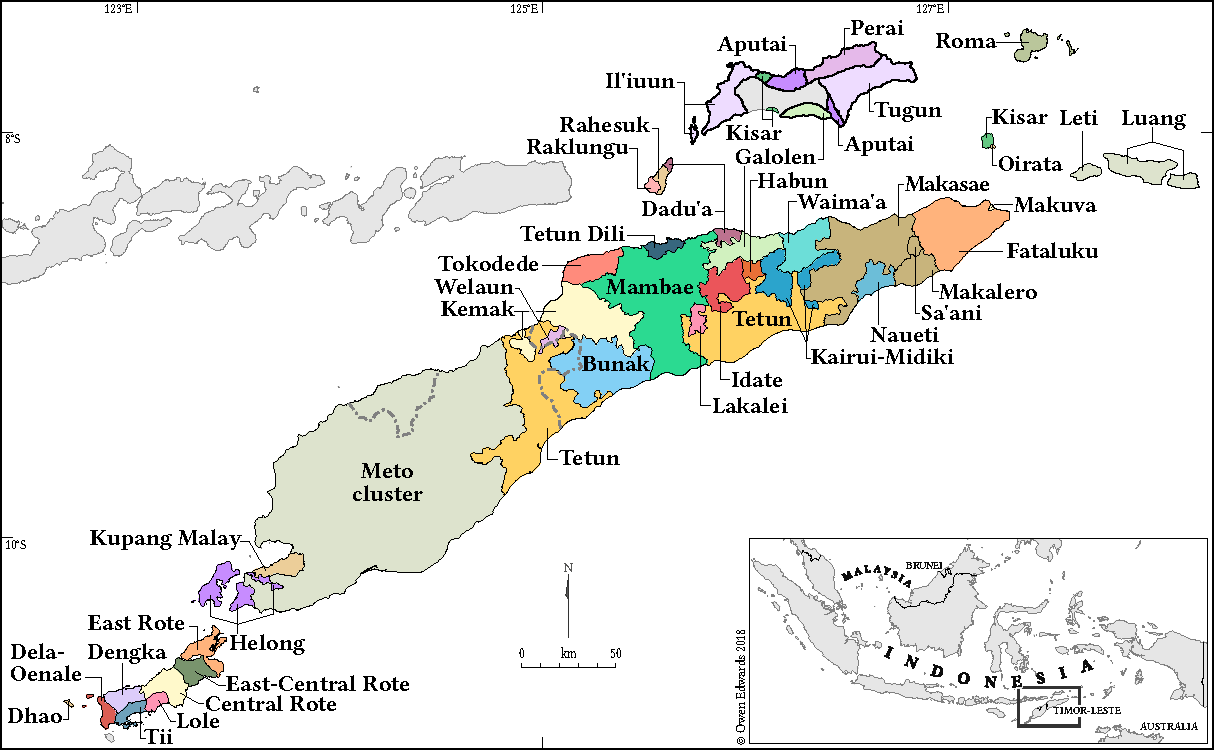
\includegraphics[width=\columnwidth]{TimorLanguages-LinLib.pdf}
\end{figure}

Meto speakers think of their speech as a single language
and call it \it{(uab) metoʔ}, \it{(bahasa) timor}
or occasionally \it{(bahasa) dawan}.
Speakers also recognize more than a dozen named varieties of Meto.
These varieties themselves have named dialects,
with further differences found between different villages and hamlets of a single dialect.
A map of self-identified Meto varieties is given in \frf{fig:SelIdeVarUabMeto}.

\begin{figure}[ht]
	\caption{Self-identified varieties of Meto}\label{fig:SelIdeVarUabMeto}
	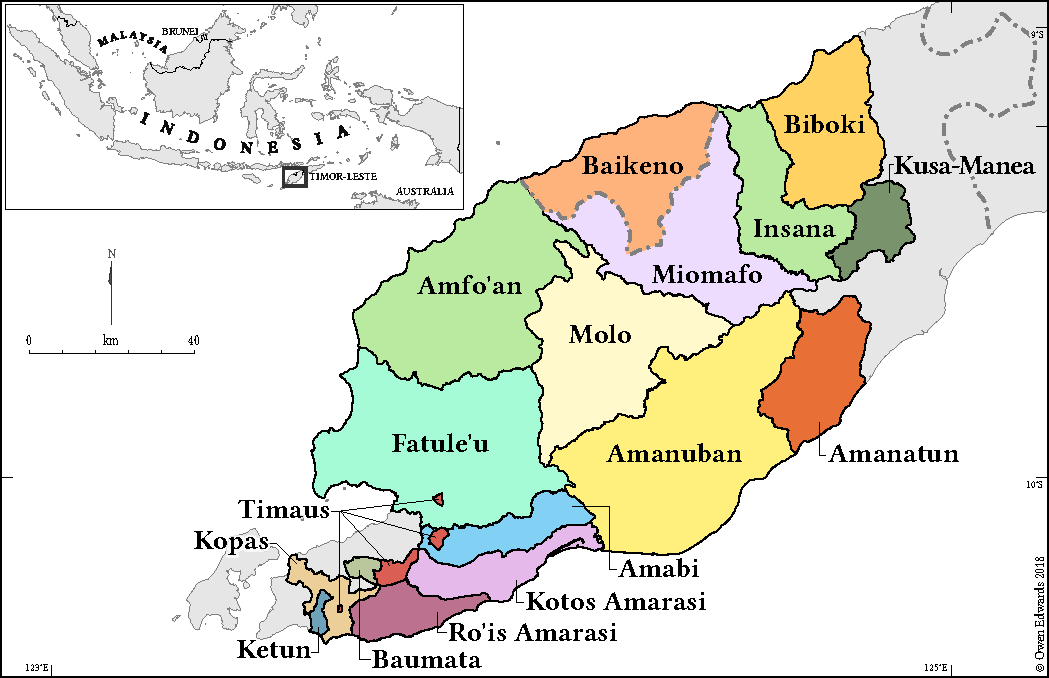
\includegraphics[width=\columnwidth]{Metos-LinLib.pdf}
\end{figure}

The borders of the self-identified varieties of Meto shown in \frf{fig:SelIdeVarUabMeto}
match closely the borders of the pre-colonial political kingdoms of western Timor.\footnote{
		The main exceptions are Kusa-Manea, which was
		part of the Tetun speaking Wehali kingdom,
		as well as Timaus, Baumata, Kopas, and Ketun, which all
		appear to be the result of migrations from more northerly areas.}
The extent to which these boundaries follow linguistic differences is unknown.
In reality, the Meto cluster is a complex language/dialect chain,
and is comparable to more well known cases such as the German chain or the Romance chain.
The nature and extent of variation among Meto varieties has not been fully studied.
Phonological, lexical, semantic, and grammatical diversity is not insignificant
and speakers frequently report difficulty communicating with speakers of other varieties.
As a result, Meto speakers of different varieties often
use a mixture of Meto and Indonesian/Kupang Malay in order to communicate.

\subsection{Affiliation}
Within Austronesian, Meto belongs to the Malayo-Polynesian subgroup
which includes all Austronesian languages outside of Taiwan.
It would further belong to Central Malayo-Polynesian
within Central-Eastern Malayo-Polynesian
\citep{bl81,bl93,bl09b} but the extent
to which these constitute valid
linguistic subgroups is contested \citep{ro95,ad05,dogr08}.

Closer to home, the nearest genealogical relative of Meto is the Rote cluster
spoken on the island of Rote just to the south-west of Timor.
Based on shared sound changes, Rote-Meto can be placed in a Timor-Babar
subgroup which contains the Austronesian languages of Timor and south-west Maluku
(from Babar island to Wetar island), though excluding
Mambae, Tokodede, Welaun, and Kemak which
form a Central Timor subgroup \citep{ed18d,ed19}.

While Meto is demonstrably Austronesian,
it has strong influence from at least one -- probably more --
pre-Austronesian languages of the region \citep{ed16c,ed18b}.
This substrate is reflected at all levels of the language:
lexicon, phonology, morphology, and syntax.

Typologically, Meto fits well in the Melanesian linguistic area with four to five
of the six properties identified by \cite{sc15} as constituting this area.
The only property of linguistic Melanesia which Meto unambiguously lacks
is that of having complex numerals below ten.
Apart from this Meto has genitive-noun order,
absence of velar nasal /ŋ/, noun-numeral order
and possessive classification,
all of which are typical of linguistic Melanesia.

Another property of linguistic Melanesia is verb-negator order.
Regarding this property, most varieties of Meto
for which data is available have double negation
with \ve{ka=} occurring before the verb and \ve{=fa} after the verb.
However, Ro{\Q}is Amarasi has post-verbal \ve{=maeʔ}
while Amfo{\Q}an only has pre-verbal \ve{ka=}.

While Meto fits well within linguistic Melanesia,
it is, based on current understanding,
only a peripheral member of linguistic Wallacea as identified by \cite{sc15}.
\citeauthor{sc15} gives four properties of linguistic
Wallacea: cognates of \su{\#}muku `banana', neuter gender,
semantic alignment, and synchronic metathesis.
Of these, Meto only has synchronic metathesis.

\subsection{Amarasi}\label{sec:Amarasi}
Amarasi is spoken towards the south-west end of the Meto speech area.
One salient feature which sets Amarasi apart from most other Meto
varieties is the liquid /r/ instead of /l/;
most Meto varieties have only a single liquid.\footnote{
		Amabi also has /r/ instead of /l/ as does
		Kusa-Manea, though /l/ occurs in many Tetun loanwords in Kusa-Manea.
		Timaus has both /l/ and /r/ due to a *{\j} > /r/ sound change.}

Amarasi speakers identify three Amarasi dialects: Kotos, Ro{\Q}is, and Tais Nonof.
Current data indicates that Tais Nonof is a label for the speech of
those living along the coast of the Amarasi area,
including those whose speech is most similar to Kotos Amarasi
and those whose speech is most similar to Ro{\Q}is Amarasi.
Amarasi speakers also report that the Amabi variety of Meto
is very similar to their own speech with minor lexical differences.

Differences between Kotos Amarasi and Ro{\Q}is Amarasi
include different functors (grammatical morphemes),
lexicon, phonotactics, as well as having undergone different sound changes.
A number of functors in Ro{\Q}is and Kotos Amarasi
are shown in Table \ref{tab:DifKotRoqFun}
as a sample of the divergence between these two lects.

\begin{table}[h]
	\caption{Different Kotos and Ro{\Q}is functors}\label{tab:DifKotRoqFun}
		\begin{tabular}{lll|lll}
		\lsptoprule
				Kotos 		&Ro{\Q}is 			&gloss		&Kotos 			&Ro{\Q}is 	&gloss	\\ \midrule
				\ve{he}		&\ve{nu}				&{\he}		&\ve{ia}		&\ve{ai}		&{\ia}	\\
				\ve{reʔ}	&\ve{heʔ}				&{\req} 	&\ve{nee}		&\ve{nae}		&{\nee} \\
				\ve{ka={\ldots}=fa}
									&\ve{maeʔ}			&{\kaah}	&\ve{iin}		&\ve{hiin}		&{\iin}	\\
				\ve{on}		&\ve{en}				&{\on}		&\ve{=een}	&\ve{=heen}	&{\een} \\
				\ve{n-bi}	&\ve{n-biʔaak}	&{\bi}		&\ve{nai}		&\ve{neu}		&already \\
				\ve{et}		&\ve{ek/et}			&{\et}		&\ve{u-}		&\ve{ku-}		&{\qu}	\\
				\ve{n-ak}	&\ve{tauʔ/n-ak}	&{\ak}		&\ve{-k}		&\ve{-r}		&\tsc{3pl.gen}\\
				\ve{n-eu}	&\ve{n-uu}			&{\eu}		&\ve{a-{\ldots}-t}&\ve{ka-{\ldots}-t}&\tsc{\at}\\
			\lspbottomrule
		\end{tabular}
\end{table}

In fact, looking only at linguistic structures
and shared sound changes, Kotos Amarasi is more closely
related to other varieties of Meto than it is to Ro{\Q}is Amarasi.
Nonetheless, speakers of Kotos and Ro{\Q}is
self-identify their speech as more similar to one another
than to other Meto varieties.
They frequently interact together
and both share a common history as members of the Amarasi kingdom.
Thus, from a socio-historical perspective,
Kotos and Ro{\Q}is can be considered
``dialects'' of a single language.\footnote{
	Kotos and Ro{\Q}is speakers perceive their speech
	as closer to one another based on salient commonalities
	not found in nearby varieties of Meto.
	Such commonalities include /r/ instead of /l/ and
	lexical items, such as \ve{koʔu}
	`big' instead of \ve{ʔnaek}, or
	\ve{n-kono} `keep going' instead of \ve{n-fini}.}

Data from Kotos Amarasi forms the basis of this book.
I present Ro{\Q}is Amarasi data at various points when it bears on the analysis
of Kotos Amarasi and/or differs in important respects.
My Kotos data comes mostly from the hamlet \emph{(kampung)} Koro{\Q}oto,
in the modern village \emph{(desa)} Nekmese{\Q}.
My Ro{\Q}is data comes from the hamlet
of Suit in the village of Buraen, as well as the hamlets
of Batuna and Ruanrete in the village of Tunbaun.
The locations of these villages within the Amarasi
speech area are shown in \frf{fig:LocNekBurTun}.

\begin{figure}[ht]
	\caption{Locations of Nekmese{\Q}, Buraen, and Tunbaun}\label{fig:LocNekBurTun}
	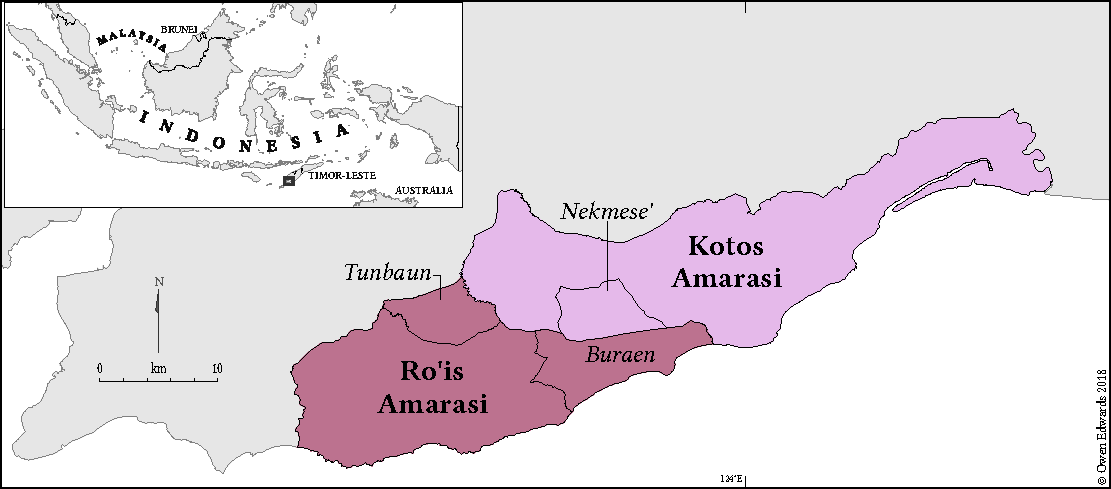
\includegraphics[width=\columnwidth]{Amarasis-LinLib.pdf}
\end{figure}

From 1968--1975 west Timor underwent an administrative restructure
with the creation of the administrative units of districts
(\emph{kecamatan}) and villages (\emph{desa}).
In Amarasi 60 hamlets were amalgamated into 23 villages.
In parts of Amarasi this amalgamation was also accompanied by the 
physical relocation of traditional hamlets in order to allow
for a more efficient development of infrastructure and delivery of services.

Nekmese{\Q} -- data from which forms the core of this work --
was created by the amalgamation of four hamlets:
Koro{\Q}oto, Fo{\Q}asa{\Q}, Tuamese{\Q} and Naet.
These hamlets still exist as \emph{dusun}
(the administrative level below \emph{desa})
and form the basis of the parishes of the dominant
Christian denomination in the village
(the protestant GMIT church\footnote{
		GMIT is an acronym of \emph{Gereja Masehi Injili di Timor};
		for which the official translation is `The Evangelical Protestant Church of Timor'.
		There are four GMIT parishes in Nekmese{\Q}:
		one serving Koro{\Q}oto, one for Fo{\Q}asa{\Q} and Tuamese{\Q}, and two for Naet.})
People also maintain their gardens and fields in the vicinity of the old hamlets.\footnote{
		Inhabitants of Koro{\Q}oto have moved the furthest,
		with \emph{desa} Nekmese{\Q} being located close to the original locations
		of Fo{\Q}asa{\Q} and Tuamese{\Q}.
		The inhabitants of Naet have moved from their original location
		towards Nekmese{\Q}, but Naet remains dislocated from the rest of Nekmese{\Q}.
		The inhabitants of Naet speak the Tais Nonof variety of Amarasi.}

Despite the administrative and physical restructure of 1968--1975,
the traditional hamlets of Nekmese{\Q} are alive and well as distinct social and linguistic units.
A summary of the speech variety which is the focus of this work is given in \qf{ex:SpeVar} below.
Unless explicitly labelled otherwise,
all data is Kotos Amarasi from the hamlet of Koro{\Q}oto.

\begin{exe}
	\ex{
		\begin{xlist}
			\ex{Language: \emph{Meto}}
			\ex{Variety: \emph{Amarasi}}
			\ex{Dialect: \emph{Kotos}}
			\ex{Hamlet: \emph{Koro{\Q}oto}}
		\end{xlist}
	}\label{ex:SpeVar}
\end{exe}

\section{Previous work}\label{sec:PreWor}
The earliest description of Meto known to me is \cite{mu57},
which contains a wordlist in what is probably a variety of Molo.
After this, the next earliest work is \cite{kl94}
which contain what appears to be an Amanuban wordlist,
though forms from other varieties are also given.

There are also works by the Dutch linguist
J. C. G. Jonker which contain data on Meto.
This includes \cite[270f]{jo04} which is a one page
glossed Amfo{\Q}an text with notes.
\cite{jo06} discusses word-final consonants in a number of
Austronesian languages including Meto.
The Meto data in \cite{jo06} is mostly Amfo{\Q}an, though data on
other varieties, including Amarasi, is also given.
Much of \citeauthor{jo06}'s Meto data also
occurs in etymological notes in \cite{jo08};
an 805-page dictionary of the Termanu variety of the Rote cluster.

\cite{ca44} provides a wordlist in Meto ``from Dutch sources''.
This appears to be based on Jonker's data
and \cite{jo06} is the source for
the discussion of final consonants in \cite[29]{ca44c}.

The first in depth treatment of Meto is that
of the Dutch missionary Pieter Middelkoop.
\citeauthor{mi39} published a collection of Amarasi texts \citep{mi39}
which had been previously collected by Jonker, a collection
of funeral chants \citep{mi49}, and a sketch grammar of Molo \citep{mi50}.
The other work by Middelkoop is an unpublished 673-page draft dictionary of Molo,
which was still in preparation before his death \citep{mi72}.\footnote{
		Thanks goes to James Fox for giving me his copy of \cite{mi72}.}
\citeauthor{mi39}'s materials on Meto contain much valuable data.
However, the transcription employed by \citeauthor{mi39} is not phonemic
and certain contrasts are under-represented.
%In order to assist future researchers I give
%here the most common transcriptional issues one encounters
%when working with \citeauthor{mi39}'s material.
%
%\begin{itemize}
	%\item The glottal stop /ʔ/ is often written as <{\Q}> between two vowels.
				%Word initially, before consonants, and word finally it is not usually written.
	%\item In \cite{mi39,mi50} the grave accent sometimes marks double vowels,
				%and sometimes phonetic vowel quality and/or stress.
				%In particular the mid-low allophone [ɛ] of /e/ is usually written \it{<è>}
	%\item A final apostrophe in \cite{mi72} marks a double vowel.
	%\item Both /ao/ and /au/ are transcribed \it{<au>}.
	%\item Prefixes consisting of a single consonant are often written
				%with a previous vowel-final word.
	%\item The final vowel of the pronouns \ve{ina} `{\iin}', \ve{sina} `{\siin}', \ve{hita} `{\hiit}'
				%is usually written with a following inflected verb.
%\end{itemize}

There are also a number of papers on Meto by Hein Steinhauer,
who worked on the Nilulat dialect of Miomafo.
This includes a description of verb morphology \citep{st93}
and a series of papers which provide an initial
description of the form of metathesis within the noun phrase
\citep{st96,st96b,st08}.

Other works which I have been able to access
on Meto include a Masters Thesis on Miomafo \citep{ta88},
a grammar produced by the Indonesian Pusat Bahasa \citep{ta89},\footnote{
		Thanks goes to Patrick McConvell for providing me
		with his copies of \citet{ta88} and \citet{ta89}.}
a description of quantification in Amanuban \citep{mebe14},
an Optimality Theory account of the segmental phonology of Miomafo \citep{is13},
a description of consonant insertion in Nai{\Q}bais Amfo{\Q}an \citep{cu18},
and a discussion of serial verb constructions in Amarasi
as being one source of similar constructions in Kupang Malay \citep{jagr11}.

\section{Data for this work}\label{sec:Meth}
The core of the Amarasi data on which this work is based
is a corpus of recorded texts totalling nearly nineteen hours
of which about five hours has been processed.
This includes a little more than three hours of
transcribed, translated, and glossed Kotos texts,
as well as just over two hours of transcribed and translated Ro{\Q}is texts.
These texts are of a variety of genres and include narratives, folk-tales,
conversations, and traditional poetry.

An index of the texts which comprise this corpus is given in Appendix
% \ref{app:TexInd}.
D.
These texts are archived with the
Pacific And Regional Archive for Digital Sources in Endangered Cultures (PARADISEC)
and nearly all are freely downloadable.

My Kotos texts were collected in three
field trips totalling seven months I made
in 2013, 2014, and 2016 over the course of my PhD work.
During these field trips I was hosted in Timor by
Heronimus Bani (Roni), a native speaker of Amarasi, in the village of Nekmese{\Q}.
These texts were recorded either by me or by Roni
and then transcribed and translated by native speakers of Amarasi, either Roni or Yedida Ora (Oma).
I then checked the initial transcriptions against the recording and glossed the text in Toolbox.
All my Kotos Amarasi texts can be accessed
from \url{http://catalog.paradisec.org.au/collections/OE1}.

During 2012 I was a participant in a two week
language documentation workshop held in Kupang:
\emph{Preserving Knowledge through Recording and Writing Local Languages}.
During this workshop a number of additional Kotos Amarasi
texts were recorded and transcribed by Oma.

My Ro{\Q}is texts were collected during a
field trip at the end of 2018
while undertaking an Australia Awards Endeavour Fellowship.
During this trip I spent one week in Buraen
with Toni Buraen and his family, followed by
two weeks in Tunbaun with Melianus Obhetan and his family.
I transcribed my Ro{\Q}is Amarasi texts
and then checked them with native speakers.
My Ro{\Q}is Amarasi texts can be downloaded from
\url{http://catalog.paradisec.org.au/collections/OE2}.

In addition to this text corpus, I also conducted a number of
elicitation sessions with Roni in 2016.
This elicitation involved working through recorded texts with Roni
and manipulating individual parts of sentences for grammaticality judgements.
When a manipulated sentence was accepted as grammatical,
I would then have Roni say it back to me.
This often resulted in him rejecting a sentence he had originally accepted.
Elicitation was also carried out with Oma on a number of occasions.

This data is supplemented by a translation
of the New Testament and Genesis into Kotos Amarasi: \citet{UBB15}.\footnote{
		This translation can be accessed online at \url{www.e-alkitab.org}
		or downloaded for free on Android devices from Google Playstore (search: Amarasi Bible).}
This translation was carried out by native Amarasi speakers
and is completely natural and idiomatic Amarasi as evidenced
by the fact that it is full of grammatical constructions that differ
from both Indonesian and Kupang Malay (used as front translation).
Before publication this translation was checked with at least three different
groups of native speakers comprising three or more speakers in each group
(representing a good cross section of age, gender, and educational levels) for clarity and naturalness.
The material was tested and further refined with each successive group,
then followed by a smoothing read-through looking at naturalness and flow before publishing.

Data from this translation is presented
when it contains good, clear exemplars of rare constructions.
However, no part of my analysis rests
solely on data found only in the Amarasi Bible translation.
See \cite{hehawi11} and \citet[2]{dryer13} for discussion of
the use of Bible translations as sources of linguistic data.

A final source of Kotos Amarasi data is a series
of primary school readers translated from Kupang Malay
into Amarasi by Yedida Ora \citep{or16,or16b,or16c}.
These readers have also been checked and edited for naturalness and fluency.

In addition to all this Amarasi data, I also have also
collected data on the following varieties of Meto,
some of which appears at various points in this book:
Timaus (half an hour of transcribed, translated, and glossed texts,
as well as 1 hour 15 minutes untranscribed texts, lexicon of 685 headwords),
Kusa-Manea (four hours of untranscribed texts, lexicon of 488 headwords),
Amanuban (22 untranscribed texts, 8 wordlists),
Ketun (3 untranscribed texts, 3 wordlists),
Kopas (3 untranscribed texts, 5 wordlists),
Fatule{\Q}u (2 wordlists), and
Amfo{\Q}an (1 wordlist).
I also have Baikeno data collected during
the 2012 Kupang language documentation workshop,
as well as data collected and provided by Charles Grimes.
Unless otherwise cited, all Meto data in this book comes
from these sources.

\section{Presentation of data and notational conventions}\label{sec:PreDat}
Data from Amarasi, or another variety of Meto,
is transcribed phonemically and presented in italic font.\footnote{
		There are only three non-phonemic aspects of my transcription.
		Firstly, foreign proper names are transcribed orthographically
		when they contain non-native phonemes the IPA representation
		of which is not identical to their orthographic, e.g. \ve{Lince} [li{\ny\tS}e].
		Secondly, /ɡw/ is transcribed \it{<g>} before rounded vowels (\srf{sec:VoiObs}).
		Thirdly, /n/ {\ra} [ŋ] is transcribed \it{<ng>} when it occurs before /ɡw/
		without an intervening morpheme break.
		These last two non-phonemic conventions
		can be seen in the word for `teacher',
		which according to my analysis has the form /tunɡwuru/,
		but is transcribed as \ve{tuŋguru}.}
Example sentences are given with up to two gloss lines.
A typical example is given in \qf{ex:120715-4, 0.55 ch:Intr} below.

\begin{exe}
	\ex{\glll	\sf{ahir{\ny}a} ahh, n-aim naan baar\j=esa =m na-maikaʔ n--\\
						\sf{ahir{\ny}a} {} n-ami naan bare=esa =ma na-maikaʔ {}\\
						in.the.end {} 3-look.for{\M} {\naan} place{\Mv}={\es} =and {\na}-settle {}\\
			\glt	`In the end, he looked there for a place and settled.'
						\txrf{120715-4, 0.55} {\emb{120715-4-00-55.mp3}{\spk{}}{\apl}}}\label{ex:120715-4, 0.55 ch:Intr}
\end{exe}

The first line is the phonemic transcription with morpheme breaks indicated.
Affixes are separated by the hyphen -.
Enclitics are separated from their host by the equals sign =.
Vowel initial enclitics which induce morphophonemic processes on their
host (Chapter \ref{ch:PhoMet}), are attached directly to the host,
while other enclitics are offset.
An example of each kind of enclitic can be seen in \qf{ex:120715-4, 0.55 ch:Intr}
with vowel initial \ve{=esa} `one' and consonant initial \ve{=m} `and'.

Word-initial epenthetic /a/ is separated by the vertical line |.
The underscore {\gap} is used to separate two parts of a phrase with
a non-compositional meaning or phrases where
one element does not occur independently.
An example of epenthesis occurs in \ve{a|n-kobub}
`piled up' in \qf{ex:120715-4, 0.05 ch:Int} below,
and an example of a non-compositional phrase is
\ve{paha{\gap}ʔpinan} `country{\gap}below' = `world'
in \qf{ex:120715-4, 0.05 ch:Int}.

Instances of Indonesian/Kupang Malay code-switching or unassimilated loans 
are transcribed in a sans-serif typeface.
Thus, in example \qf{ex:120715-4, 0.55 ch:Intr} the word
\ve{\sf{ahir{\ny}a}} `in the end' is from Kupang Malay \it{ahirnya}.
Phonetic strings which are pauses are indicated by a final \it{<hh>} and are usually unglossed.
In example \qf{ex:120715-4, 0.55 ch:Intr} \ve{ahh} is a pause
with the phonetic quality approximating [aːː],
similarly \ve{nehh} is a pause which sounds like [nɛːː].
False starts are not glossed and indicated by a final en-dash --.
One example is the final \ve{n--} in example \qf{ex:120715-4, 0.55 ch:Intr} above.
Commas indicate pauses and/or intonation breaks
and full stops represent the end of an intonation unit.
Capital letters are only used for proper names.

The second line gives the underlying form
of morphemes before processes of metathesis, consonant insertion, and vowel assimilation occur.
It also gives the underlying forms of enclitics which have multiple forms (\srf{sec:SenEnc}).
The third line gives the morpheme by morpheme gloss.
When a morpheme is ambiguous between several values,
these values are separated by a slash /. An example
is the verbal agreement prefix \ve{m-} `{\m}' which
agrees with first person exclusive,
second person singular, and second person plural.
Glosses mostly follow the Leipzig Glossing Rules
with a full list of glosses used in this book,
including non-standard glosses, given beginning on \prf{ch:Abb}.

\begin{table}[ht]
	\caption{Glosses for U-forms and M-forms}\label{tab:GloUfoMfo}
		\begin{tabular}{ll}
			\lsptoprule
						Gloss & Use \\ \midrule
				\tsc{u}		& U\=/form \\
				%\tsc{u\shiftleft{1.3pt}{\scalebox{2.0}{ͨ}}}		& 1. U\=/form of consonant-final stem\\
				\tsc{u\raisebox{-4pt}{\scalebox{1.75}{ͨ}}}		& 1. U\=/form of consonant-final stem\\
									& 2. U\=/form before consonant cluster\\
				\tsc{m}		& M\=/form\\
				\tsc{m\shiftleft{0.8pt}{̿}}		& M\=/form before vowel-initial enclitic \\
				\tsc{m\shiftleft{0.25pt}{\raisebox{-4pt}{\scalebox{1.75}{ͨ}}}}		& M\=/form before consonant cluster\\
			\lspbottomrule
		\end{tabular}
\end{table}

Glosses indicating U\=/forms and M\=/forms
are usually only given when potentially relevant to the discussion at hand.
Glosses for U\=/forms and M\=/forms in different phonotactic environments are given in \trf{tab:GloUfoMfo},
with a number of examples given in \qf{ex:120715-4, 0.05 ch:Int}--\qf{130821-1, 6.20} below.
See Chapter \ref{ch:StrMetAma} for more discussion of the distribution
of each of these forms.
Glosses for U\=/forms or M\=/forms are not given when a form
does not distinguish between them.

\begin{exe}
	\ex{\glll	neno naa paha{\gap}ʔpina-n ia, a|n-kobub on bare meseʔ\\
						neno naa paha{\gap}ʔpina-n ia	{\a}n-kobub on bare meseʔ\\
						day{\tbrU} {\naa} land{\gap}below{\tbrU}-{\N} {\ia} {\a\n}-pile{\tbrUc} {\on} place{\tbrU} one\\
			\glt	`In those days the world was piled up in one place.'
						\txrf{120715-4, 0.05} {\emb{120715-4-00-05.mp3}{\spk{}}{\apl}}}\label{ex:120715-4, 0.05 ch:Int}
	\ex{\glll	uma ʔ-tee =ma, ʔ-aiti bruuk.	\\
						uma ʔ-tea =ma ʔ-aiti bruuk \\
						{\uma\tbrUc} \q-arrive =and \q-pick.up{\tbrUc} pants{\U}	\\
			\glt	`I arrived (home) and picked up some pants.'
						\txrf{130825-6, 10.05} {\emb{130825-6-10-05.mp3}{\spk{}}{\apl}}}\label{130825-6, 10.05 ch:Int}
	\ex{\glll	hii m-euk siis\j=ii =m	\\
						hii m-eku sisi=ii =ma\\
						{\hii} \m-eat{\tbrM} meat{\tbrMv}={\ii} =and	\\
			\glt	`You ate the meat and' \txrf{120923-1, 6.01} {\emb{120923-1-06-01.mp3}{\spk{}}{\apl}}}\label{120923-1, 6.01}
	\ex{\glll	afi{\gap}naa au ʔ-tae iin sura srainʔ=ii =t	\\
						afi{\gap}naa au ʔ-tae ini surat sraniʔ=ii =te	\\
						yesterday {\au} ʔ-look.down {\iin} paper{\tbrMc} baptism{\tbrMv}={\ii} ={\te}\\
			\glt	`Yesterday when I looked at her baptismal certificate,'
						\txrf{130821-1, 6.20} {\emb{130821-1-06-20.mp3}{\spk{}}{\apl}}}\label{130821-1, 6.20}
\end{exe}

Gloss lines are followed by a free translation into English.
Words not present in the Amarasi example
but supplied in the free translation to increase
its naturalness are enclosed in brackets ().
Important para-linguistic information such as gestures
are described in square brackets [] in the free translation.
Occasionally a literal translation of part or all of the Amarasi example is given.
Literal translations are enclosed in brackets and preceded by the abbreviation `\emph{lit.}'.

The numeric code to the right of the free translation
is a reference to which text the example comes from.
These codes follow the format \emph{yy-mm-dd-no., time in text}.
Thus, the code {\ttfamily 120715-4, 0.55} in example \qf{ex:120715-4, 0.55 ch:Intr} above
indicates that this example begins at about 55 seconds
into the fourth recording made on the 15/07/2012.

Examples with the speaker icon \spk{}
have an accompanying sound file.
These
sound files can be downloaded from TROLLing (The Tromsø Repository of Lan-
guage and Linguistics) at \url{https://doi.org/10.18710/IORWF6}  \citep{ed20}. These
sound files are organised in the repository according to the chapter in which they
occur with additional information on their specific location, such as example or
table number, embedded in the file name. See the ReadMe in the TROLLing repos-
itory for a complete explanation.


In addition to examples from my text collection,
three other kinds of examples occur.
Firstly, data which was encountered during the course
of my fieldwork but not recorded is indicated as \emph{observation}
usually with the date and page reference to my notebook; e.g. {\ttfamily observation 09/10/14, p.113}.
Secondly, data which were collected during elicitation are marked as \emph{elicit.}
with the date and page reference to my notebook; e.g. {\ttfamily elicit. 15/03/2016 p.47}
Finally, data from the Amarasi Bible translation are referenced
by book, chapter, and verse, e.g. {\ttfamily John 3:16}.

When longer examples from a single text are given,
a short description usually precedes the text
(followed by the unique code cross referencing the text).
The data following this title is then labelled alphabetically.
An example is given in \qf{ex:120715-4, 0.43-0.45 ch:Intr} below.
When an example involves more than one speaker,
different speakers are indicated with Greek letters.

\largerpage
\begin{exe}
	\ex{How Moo{\Q}-hitu made the world:
				\txrf{120715-4} {\emb{120715-4-00-43-00-45.mp3}{\spk{}}{\apl}}}\label{ex:120715-4, 0.43-0.45 ch:Intr}
	\begin{xlist}
		\ex{\glll	n-bi{\tl}bi oo\j=ee naan-n=ee {onai =te},\\
							n-bi{\tl}bi oe=ee nana-n=ee {onai =te}\\
							\n-{\prd}{\bi} water={\ee} inside-{\N=\ee} and.then\\
				\glt	`Having been in the water for a while,' \txrf{0.43}}\label{ex:120715-4, 0.43 ch:Intr}
\clearpage
		\ex{\glll	a|n-moʔe =ma n-poo\j=ena n-bi metoʔ.\\
							{\a}n-moʔe =ma n-poi=ena n-bi metoʔ\\
							{\a\n}-make =and \n-exit={\een} {\n}-{\bi} dry\\
				\glt	\lh{a|}`(he) made and went out onto dry land.' \txrf{0.45}}\label{ex:120715-4, 0.45 ch:Intr}
	\end{xlist}
\end{exe}

When data on languages other than Amarasi or Meto is cited,
such data is transcribed in italics phonemically according to IPA conventions.\footnote{
		For the sake of complete clarity, the palatal glide /j/
		is always transcribed \it{<j>} while the 
		palatal affricate /\j/ is always transcribed \it{<\j>}.}
Data from languages with a widely used standard
orthography are usually transcribed orthographically followed
by a phonemic IPA transcription, an example is English \it{mouse} /maʊs/.

\section{Goals and the use of theory}\label{sec:GoaUseThe}
The main goal of this book is to present an accurate
description of the forms and functions of metathesis in Amarasi
(chapters \ref{ch:StrMetAma}--\ref{ch:DisMet}).
A secondary goal is to propose a clear analysis of the data.
A third goal to situate the Amarasi data within
its typological, geographical, and cultural context
(Chapters \ref{ch:SynchMet} and \ref{ch:ConCon})

Notably, it is \emph{not} the main goal of this book to
present the Amarasi data as an argument in
favour of any particular theoretical model.
While I make frequent use of representations and
tools from different theoretical models,
I do so mainly to illustrate clearly
aspects of the Amarasi data in a helpful way
and as explicit strategy to summarise certain generalisations.

Thus, in Chapters \ref{ch:StrMetAma} and \ref{ch:PhoMet}
I make use of Autosegmental theory as it helpfully
illustrates the processes which occur in the derivation of M\=/forms from U\=/forms.
Similarly, in describing M\=/forms before consonant clusters
\srf{sec:CCIniMod} I make use of Optimality Theory
as the tableaux of this theory illustrate well the large
number of potential outputs a particular string could generate.
Likewise, in Chapter \ref{ch:SynMet} I make use of X-bar theory to analyse
the role of metathesis within the syntax.

In general, different theoretical models
and the analyses these entail are deployed in this book
in an expedient manner according to what seems most
illuminating for the Amarasi data.
The primary use of theory is to present a clear and simple
analysis of Amarasi metathesis,
not a theoretically consistent analysis.
Thus, the observant reader will note, for instance,
that in my account of phonologically conditioned metathesis
in Chapter \ref{ch:PhoMet} I make frequent use of
constraints developed within Optimality Theory
without ever presenting an Optimality Theory tableau.
While I find some Optimality Theory constraints helpful
in understanding the data, an actual account embedded within Optimality Theory
clouds rather than illuminates the description.\footnote{
		This is not to say that Optimality Theory is wrong,
		or that it cannot or should not be used to analyse Amarasi metathesis.
		Instead, I merely do not find a full Optimality Theory account
		of this aspect of Amarasi metathesis a helpful aid.}

The main exception to this approach is in the analysis
of the structure of metathesis in Chapter \ref{ch:StrMetAma}.
In this chapter I explicitly formulate an analysis
using an autosegmental model of phonology \citep{go76}
and a rule-based model of process morphology \citep{ma74,an92}.
I do this because these models allow me to propose a
unified analysis of the form of Amarasi metathesis.

However, my primary commitment is not to any particular theory,
or any particular analysis, but to the Amarasi data itself.
I would welcome criticism of the analyses
proposed in this book so long as any alternate analyses
remain faithful to the primary data upon which any analysis must be based.
Similarly, I would welcome any dialogue with this book
which attempts to provide a unified theoretical account of all of the data.
\section{Terminology}\label{sec:Ter}
In this section I give definitions of potentially ambiguous linguistic terminology.
The definitions given here should be taken only as a practical guide
to understand how terms are used in this book
and should \emph{not} be taken as strong claims
about the theoretical status of any of the elements defined.

As used in this book, a \emph{word} is the minimal meaningful
phonological string which can occur in isolation.\footnote{
		Two typical environments in which words occur in isolation are
		in response to a question or in collection of a wordlist.
		Likewise, pauses are not usually allowed in the middle of a word.
		If such a pause occurs, the speaker usually repeats the entire word from the beginning.}
A \emph{morpheme} is ``an indivisible stretch of phonetic (or phonological)
material with a unitary meaning'' \citep[49]{an92}.\footnote{
		In many morphological theories the morpheme does not play a central role,
		including \cite{ma74,an92} and \cite{st01}.
		While I am extremely sympathetic to such theories,
		the morpheme is still a useful analytic tool for much of the Amarasi data.}
A \emph{root} is an underlying single morpheme without any affixes attached.

We can furthermore distinguish between \emph{bound} and \emph{free morphemes}.
A free morpheme is a root which can occur as a word without any other morphemes attached.
A typical example is \ve{kaut} `papaya'.
A bound morpheme is a root which cannot occur as a word.
Instead a bound morpheme must surface attached to another morpheme.
A \emph{clitic} is a morpheme which is phonologically bound
to a clitic host, but has a separates syntactic status to the host.
A typical example is the determiner \ve{=ee}, which marks definiteness.
While this determiner must occur attached to a host (e.g. \ve{kaut=ee} `the papaya')
which is the head of a noun phrase, the enclitic itself 
is the head of a separate determiner phrase (\srf{sec:DetPhr}).
My definitions of all these terms when applied to Amarasi or Meto data
are summarised in \qf{ex:TerDef} below, with a number of examples also given.

\begin{exe}
	\ex{Terminological definitions \txrf{}}\label{ex:TerDef}
	\begin{xlist}
		\ex{Morpheme = indivisible phonetic stretch with unitary meaning}
			\sn{\ve{n-} `third person verbal agreement', \ve{kobub} `pile up', \ve{kaut} `papaya', \ve{=ee} `{\ee}, third person determiner'}
		\ex{Word = minimal phonological string which can occur in isolation}
			\sn{\ve{n-kobub} `piles up', \ve{kaut} `papaya', \ve{kaut=ee} `the papaya'}
		\ex{Bound morpheme = morpheme which cannot occur as an independent word}
			\sn{\ve{n-} `third person verbal agreement', \ve{=ee} `{\ee}'}
		\ex{Root = underlying single morpheme}
			\sn{\ve{{\rt}n-} `third person verbal agreement', \ve{{\rt}kobub} `pile up', \ve{kaut} `papaya', \ve{{\rt}=ee} {\ee}}
		\ex{Free morpheme = morpheme which is an eligible word}
			\sn{\ve{kaut} `papaya', \ve{teun} `three'}
		\ex{Affix = bound morpheme with no separate syntactic status to its host}
			\sn{\ve{n-} `third person verbal agreement', \ve{-m} {\mg} `first person exclusive or second person genitive'}
		\ex{Clitic = bound morpheme with different syntactic status to its host}
			\sn{\ve{=ee} `{\ee}', \ve{=ma} `and', \ve{=kau} `{\kau}'}
		\ex{Stem = a word or root to which a bound morpheme attaches}
			\sn{\ve{n-\tbr{kobub}} `piles up', \ve{\tbr{kaut}=ee} `the papaya'}
		\ex{Citation Form = usual form of a word given in wordlist style elicitation}
	\end{xlist}
\end{exe}

I also make a distinction between two kinds of words and roots,
\emph{functors} and \emph{lexical words/roots} \citep[85ff]{zo78,gr91}.
Functors are morphemes which have grammatical uses,
such as relativisers, demonstratives, topic markers, and pronominals,
while lexical words/roots typically refer to events, states, properties, and things.


\chapter{Synchronic metathesis from a cross-linguistic perspective} \label{ch:SynchMet}

\section{Introduction}
In this chapter I discuss synchronic metathesis
from a cross-linguistic perspective.
I begin in \srf{sec:KinSynMet} with a categorisation
of the different types of synchronic metathesis
that are found in languages of the world.
Aftre this I provide a survey of languages with
synchronic metathesis in \srf{sec:SurLanMet}, focussing on those
of greater Timor -- the region where Meto is spoken.
This is followed by a discussion of the origins of
synchronic metathesis in \srf{sec:OriSynMet}, and
a summary of the forms and functions of synchronic metathesis
in \srf{sec:For ch:SynchMet} and \srf{sec:FunMorMet} respectively.

Probably the most familiar kind of metathesis is historic metathesis
in which a sequence of two sounds has swapped
position at some point in the history of the language.
One case of historic metathesis is found in Dutch
in which rhotic-vowel sequences metathesised
before certain dental consonants \citep[108]{va17}.
An example is Dutch \it{b\tbr{or}st} /b\tbr{ɔr}st/ `breast'
which can be compared with German \it{b\tbr{ru}st} /b\tbr{rʊ}st/
or English \it{b\tbr{rea}st} /b\tbr{rɛ}st/ each of
which preserves the older rhotic-vowel order.

Synchronic metathesis, on the other hand,
is when at least some words in a language
have alternate forms in certain situations
which differ in the order of some of their segments in a regular and systematic way.
Thus, in Rotuman (\srf{sec:Rot}) the word for `flower'
is either \it{ho\tbr{sa}} or \it{ho\tbr{as}} \citep[14]{ch40}.

One phenomenon excluded from my discussion in this chapter
which could be considered metathesis
is that of affixes which have both stem internal and stem external allomorphs.
One example is found in \ili{Ulwa} (Misumalpan, Nicaragua)
in which the \tsc{3sg.gen} affix \it{-ka/\<ka\>}
attaches to the first iambic foot of the stem.\footnote{
		An iambic foot in Ulwa consists of a light syllable followed by a heavy syllable,
		two light syllables, or a single heavy syllable.}
This affix surfaces as a suffix when a word consists of only a single iambic foot
and as an infix when the first iambic foot is followed by other syllables.
Examples are given in \qf{ex2:Ulw3sg} below.

\begin{exe}
	\ex{Ulwa \tsc{3sg.gen} \it{-ka} \hfill(\citealp{habl89} in \citealp{mccpr93})}\label{ex2:Ulw3sg}
	\sn{\gw\begin{tabular}{rlll}
		\it{bas} 				&\ra& \it{bas-\tbr{ka}} 					&`hair'\\
		\it{kiː} 				&\ra& \it{kiː-\tbr{ka}} 					&`stone'\\
		\it{sana}			 	&\ra& \it{sana-\tbr{ka}} 					&`deer'\\
		\it{amak}			 	&\ra& \it{amak-\tbr{ka}}				 	&`bee'\\
		\it{sapaː}		 	&\ra& \it{sapaː-\tbr{ka}} 				&`forehead'\\
		\it{suːlu} 			&\ra& \it{suː\<\tbr{ka}\>lu}			&`dog'\\
		\it{asna} 			&\ra& \it{as\<\tbr{ka}\>na}			 	&`clothes'\\
		\it{siwanak} 		&\ra& \it{siwa\<\tbr{ka}\>nak} 		&`root'\\
		\it{anaːlaːka} 	&\ra& \it{anaː\<\tbr{ka}\>laːka} 	&`chin'\\
		\it{karasmak} 	&\ra& \it{karas\<\tbr{ka}\>mak} 	&`knee'\\
		\end{tabular}}
\end{exe}

This chapter provides the typological context for my
description of metathesis in Amarasi.
Because of this, I frequently provide forward references
to later sections of this book in which Amarasi phenomena
similar to those under discussion are provided.

\section{Kinds of synchronic metathesis}\label{sec:KinSynMet}
In this section I present a categorisation of processes of synchronic
metathesis according to the environments in which they occur.
I identify three kinds of metathesis: 
phonologically conditioned metathesis (\srf{sec:PhoMet}),
morphemically conditioned metathesis (\srf{sec:MorpheConMet}),
and morphological metathesis (\srf{sec:MorMet}).
The categorisation into these three types of metathesis
is intended to facilitate an understanding of different
metathesis patterns and their systematicity.
I discuss each type of synchronic metathesis in turn
and relate them to other, more familiar, phonological processes.

It is frequently the case that a unitary analysis of synchronic
metathesis is not always possible.
Such a process of metathesis may be phonologically
conditioned in some environments, morphemically conditioned in others
and morphological in yet other situations.
This, for instance, is the situation with Rotuman metathesis (\srf{sec:Rot}).
It is also the situations in Amarasi which has
phonologically conditioned before vowel initial enclitics (Chapter \ref{ch:PhoMet}),
and two process of morphological metathesis (Chapter \ref{ch:SynMet} and Chapter \ref{ch:DisMet}).

One kind of synchronic metathesis which does not fit
into any of these three categories is when metathesised
and unmetathesised forms are in free variation.
This situation is found in Kui (Trans-New-Guinea, Alor),
in which the perfective affix \it{-i}
optionally metathesises with a previous /n/ or /l/.
Examples are given in \qf{ex:KuiPer} below.
As currently described, this alternation is a case of free variation.

\begin{exe}
	\ex{Kui metathesis of perfective \it{-i} \citep[124f]{wish17}}\label{ex:KuiPer}
	\sn{\gw\begin{tabular}{rclllllll}
		\it{alon} 	&+&\it{i}&{\ra}& \it{alon\tbr{i}}		&{\tl}& \it{alo\tbr{i}n} &`write'\\
		\it{gaman} 	&+&\it{i}&{\ra}& \it{gaman\tbr{i}}	&{\tl}& \it{gama\tbr{i}n} &`do'\\
		\it{aka:l} 	&+&\it{i}&{\ra}& \it{akaːl\tbr{i}}	&{\tl}& \it{akaː\tbr{i}l} &`eat'\\
		\it{taŋgan} &+&\it{i}&{\ra}& \it{taŋgan\tbr{i}}	&{\tl}& \it{taŋga\tbr{i}n} &`ask'\\
		\it{uban} 	&+&\it{i}&{\ra}& \it{uban\tbr{i}}		&{\tl}& \it{uba\tbr{i}n} &`talk'\\
		\it{gatan} 	&+&\it{i}&{\ra}& \it{gatan\tbr{i}}	&{\tl}& \it{gata\tbr{i}n} &`free'\\
		\end{tabular}}%vsp
\end{exe}

While this data bears some similarities to the Ulwa data
discussed above the existence of alternations
such as \it{aloni} and \it{aloin} `write-\tsc{perf}'
indicates that this is indeed a case of metathesis.
That perfective \it{-i} is a suffix
after stems without final /n/ or /l/ indicates
that infixal allomorph in examples such as those in \qf{ex:KuiPer}
is a result of CV {\ra} VC metathesis.

	\subsection{Phonologically conditioned metathesis}\label{sec:PhoMet}
Phonologically conditioned metathesis is any process of metathesis
which is an automatic result of a phonological environment.
Amarasi has a process of phonological metathesis conditioned
by vowel-initial enclitics (see Chapter \ref{ch:PhoMet}).

Processes of phonologically conditioned metathesis
are similar to other more familiar phonological processes
such as final obstruent devoicing in \ili{German}.
In German a voiced obstruent is devoiced word finally,
as can be seen from the data given in \qf{ex:GerFinObsDev} below.

\begin{exe}
	\ex{German final obstruent devoicing \hfill\citep[11f]{br95}}\label{ex:GerFinObsDev}
	\sn{\gw\begin{tabular}{lllll}
			\mc{2}{l}{Singular}					&\mc{2}{l}{Plural} 			& gloss		\\
			\it{Dieb}		&/diː\tbr{p}/		&\it{Diebe}		&/diː\tbr{b}ə/	&`thief'	\\
			\it{halb}		&/hal\tbr{p}/		&\it{halbe}		&/hal\tbr{b}ə/	&`half'	\\
	%		\it{Bord}		&/bɔr\tbr{t}/		&\it{Borde}		&/bɔr\tbr{d}ə/	&`shelf'	\\
			\it{Bund}		&/bʊn\tbr{t}/		&\it{Bunde}		&/bʊn\tbr{d}ə/	&`league'	\\
	%		\it{Sieg}		&/ziː\tbr{k}/		&\it{Siege}		&/ziː\tbr{ɡ}ə/	&`victory'	\\
	%		\it{Tag}		&/taː\tbr{k}/		&\it{Tage}		&/taː\tbr{ɡ}ə/	&`day'	\\
			\it{Zweig}	&/ʦvaɪ\tbr{k}/	&\it{Zweige}	&/ʦvaɪ\tbr{ɡ}ə/	&`twig'	\\
			\it{brav}		&/braː\tbr{f}/	&\it{brave}		&/braː\tbr{v}ə/	&`well-behaved'	\\
			\it{Gas}		&/ɡaː\tbr{s}/		&\it{Gase}		&/ɡaː\tbr{z}ə/		&`gas'	\\
	%		\it{Los}		&/loː\tbr{s}/		&\it{Lose}		&/loː\tbr{z}ə/		&`lottery ticket'	\\
	%		\it{}		&/\tbr{}/		&\it{}				&/\tbr{}ə/		&`'	\\
	%		\it{}		&/\tbr{}/		&\it{}				&/\tbr{}ə/		&`'	\\
	\end{tabular}}
\end{exe}

The standard (and simplest) analysis of this data is to propose
that voiced obstruents are devoiced finally.
A simple formal rule for German obstruent devoicing is given in \qf{ex:GerObs} below.\footnote{
		German obstruent devoicing involves additional complexities.
		See \citep[200ff]{wi96} and \cite{br95} for discussion
		of the way such complexities have been resolved.}

\begin{exe}
	\ex{\tsc{[+obstruent]} {\ra} \tsc{[-voice]} /{\_}]\sub{σ} \hfill\citep[201]{wi96}}\label{ex:GerObs}
\end{exe}

In German a phonological process (devoicing) affects a
segment in a specific phonological environment.
Similarly, in the case of phonologically conditioned
metathesis a phonological process (metathesis)
occurs in a specific phonological environment.

A simple example of phonological metathesis
is provided by \ili{Faroese} (Germanic, Faroe Islands).
In Faroese the neuter form of adjectives is formed by adding the suffix \it{-t}.
When this suffix is added to a stem which ends in /sk/,
this cluster metathesises to /ks/.
Examples are shown in \qf{ex:Farsk->ks} below.
(Such metathesis is not written in Faroese.)

\begin{exe}
\ex{Faroese sk {\ra} ks /{\_}t \hfill\citep[56]{th04}}\label{ex:Farsk->ks}
	\sn{\gw\begin{tabular}{lllllll}
		\tsc{masc} 		&					 				&\tsc{fem}& 					 		&\tsc{neut}	&								& \\
		\it{grøn-ur}	&/kɹøːnʊɹ/				&\it{grøn}& /kɹœn/ 				&\it{grønt}	& /kɹœn̥t/ 			& `green' \\
		\it{fesk-ur}	&/fɛ\tbr{sk}ʊɹ/		&\it{fesk}& /fɛ\tbr{sk}/	&\it{fesk-t}& /fɛ\tbr{ks}t/	& `fresh' \\
		\it{rask-ur}	&/ɹa\tbr{sk}ʊɹ/		&\it{rask}& /ɹa\tbr{sk}/	&\it{rask-t}& /ɹa\tbr{ks}t/	& `good' \\
		\it{týsk-ur}	&/tʰʊi\tbr{sk}ʊɹ/	&\it{týsk}& /tʰʊi\tbr{sk}/&\it{týsk-t}& /tʰʊi\tbr{ks}t/& `German' \\
	\end{tabular}}
\end{exe}

This Faroese metathesis is motivated
by a phonological constraint against having a cluster of a fricative, plosive, and another plosive in that order.
If such a cluster would occur, the fricative and plosive metathesise to prevent it surfacing,
and thereby avoid violating the obligatory contour principle.
Faroese metathesis of \it{fesk} /fɛ\tbr{sk}/ {\ra} \it{feskt} /fɛ\tbr{ks}t/
is illustrated in \qf{as:fesk->fekst} below in which \emph{F} = fricative and \emph{P} = plosive.
A similar metathesis involving fricatives and plosives is also found in Lithuanian.
\cite{huse04} provide a detailed analysis of metathesis in both Faroese and Lithuanian.

\begin{multicols}{3}
	\begin{exe}
		\ex{\begin{xlist}
			\exa{\xy
				<0em,2cm>*\as{C}="x1",<1em,2cm>*\as{V}="x2",<2em,2cm>*\as{C}="x3",<3em,2cm>*\as{C}="x4",<4em,2cm>*\as{C}="x5",
				<0em,1cm>*\as{F}="C1",<1em,1cm>*\as{V}="C2",<2em,1cm>*\as{F}="C3",<3em,1cm>*\as{P}="C4",<4em,1cm>*\as{P}="C5",
				<0em,0cm>*\as{f}="c1",<1em,0cm>*\as{ɛ}="c2",<2em,0cm>*\as{s}="c3",<3em,0cm>*\as{k}="c4",<4em,0cm>*\as{t}="c5",
				"C1"+U;"x1"+D**\dir{-};"C2"+U;"x2"+D**\dir{-};"C3"+U;"x3"+D**\dir{-};"C4"+U;"x4"+D**\dir{-};"C5"+U;"x5"+D**\dir{-};
				"c1"+U;"C1"+D**\dir{-};"c2"+U;"C2"+D**\dir{-};"c3"+U;"C3"+D**\dir{-};"c4"+U;"C4"+D**\dir{-};"c5"+U;"C5"+D**\dir{-};
			\endxy}
			\exa{\xy
				<0em,2cm>*\as{C}="x1",<1em,2cm>*\as{V}="x2",<2em,2cm>*\as{C}="x3",<3em,2cm>*\as{C}="x4",<4em,2cm>*\as{C}="x5",
				<0em,1cm>*\as{F}="C1",<1em,1cm>*\as{V}="C2",<2em,1cm>*\as{F}="C3",<3em,1cm>*\as{P}="C4",<4em,1cm>*\as{P}="C5",
				<0em,0cm>*\as{f}="c1",<1em,0cm>*\as{ɛ}="c2",<2em,0cm>*\as{s}="c3",<3em,0cm>*\as{k}="c4",<4em,0cm>*\as{t}="c5",
				"C1"+U;"x1"+D**\dir{-};"C2"+U;"x2"+D**\dir{-};"C3"+U;"x4"+D**\dir{.};"C4"+U;"x3"+D**\dir{.};"C5"+U;"x5"+D**\dir{-};
				"c1"+U;"C1"+D**\dir{-};"c2"+U;"C2"+D**\dir{-};"c3"+U;"C3"+D**\dir{-};"c4"+U;"C4"+D**\dir{-};"c5"+U;"C5"+D**\dir{-};
			\endxy}
			\exa{\xy
				<0em,2cm>*\as{C}="x1",<1em,2cm>*\as{V}="x2",<3em,2cm>*\as{C}="x3",<2em,2cm>*\as{C}="x4",<4em,2cm>*\as{C}="x5",
				<0em,1cm>*\as{F}="C1",<1em,1cm>*\as{V}="C2",<3em,1cm>*\as{F}="C3",<2em,1cm>*\as{P}="C4",<4em,1cm>*\as{P}="C5",
				<0em,0cm>*\as{f}="c1",<1em,0cm>*\as{ɛ}="c2",<3em,0cm>*\as{s}="c3",<2em,0cm>*\as{k}="c4",<4em,0cm>*\as{t}="c5",
				"C1"+U;"x1"+D**\dir{-};"C2"+U;"x2"+D**\dir{-};"C3"+U;"x3"+D**\dir{-};"C4"+U;"x4"+D**\dir{-};"C5"+U;"x5"+D**\dir{-};
				"c1"+U;"C1"+D**\dir{-};"c2"+U;"C2"+D**\dir{-};"c3"+U;"C3"+D**\dir{-};"c4"+U;"C4"+D**\dir{-};"c5"+U;"C5"+D**\dir{-};
			\endxy}		
		\end{xlist}}\label{as:fesk->fekst}
	\end{exe}
\end{multicols}

\ili{Sidamo} (Cushitic, Ethiopia) also has phonologically conditioned metathesis.
In Sidamo a cluster of an obstruent followed by a nasal is disallowed.
If such a cluster is created by the addition of morphology,
the obstruent-nasal sequence undergoes metathesis.
Examples are given in \qf{ex:SidMet} below,
with the first person plural simple perfect suffix.

\begin{exe}
\ex{Sidamo obstruent+nasal {\ra} nasal-obstruent \hfill\citep[46]{ka07}}\label{ex:SidMet}
	\sn{\gw\begin{tabular}{rlllll}
		 stem 						&& \mc{2}{l}{\tsc{1pl-s.prf1-1pl}} && \\
		\it{laʔ} 					&+& \it{-n-u-mmo}&{\ra} & \it{laʔnummo} & `see' \\
		\it{mee\tbr{d}} 	&+& \it{-\tbr{n}-u-mmo}&{\ra} & \it{mee\tbr{nd}ummo} & `shave' \\
		\it{t'oo\tbr{k'}} &+& \it{-\tbr{n}-u-mmo}&{\ra} & \it{t'oo\tbr{nk'}ummo} & `flee from' \\
		\it{bi\tbr{ʧ'}}		&+& \it{-\tbr{n}-u-mmo}&{\ra} & \it{bi\tbr{nʧ'}ummo} & `scar' \\
		\it{k'aa\tbr{f}} 	&+& \it{-\tbr{n}-u-mmo}&{\ra} & \it{k'aa\tbr{nf}ummo} & `step over/walk' \\
		\it{mi\tbr{ʃ}} 		&+& \it{-\tbr{n}-u-mmo}&{\ra} & \it{mi\tbr{nʃ}ummo} & `despise' \\
	\end{tabular}}
\end{exe}

\ili{Selaru} (Austronesian, Maluku) exhibits glide-consonant metathesis.
In Selaru, glide-consonant sequences are disallowed.
The addition of a consonant-initial suffix thus
triggers metathesis with any stem-final glide.
Examples are shown in \qf{ex:SelGC->CG} below,
with suffixes attached to glide-final stems.
The glide-final stems can be contrasted with
vowel-final stems in which no metathesis occurs.
The glide-final forms, such as \it{hatw} `rock' occur with
a final glide phrase finally or in isolation.

\begin{exe}%ʷʸ
	\ex{Selaru GC {\ra} CG \hfill\citep[22]{coco00}}\label{ex:SelGC->CG}
	\sn{\gw\begin{tabular}{rlll}
		\it{tas\tbr{j}}		+ \it{-\tbr{k}e}&{\ra}&\it{tas\tbr{kj}e}& `the rope'\\
		\it{hat\tbr{w}}		+ \it{-\tbr{k}e}&{\ra}&\it{hat\tbr{kw}e}& `the rock'\\
		\it{r-lu\tbr{j}}	+ \it{-\tbr{b}o}&{\ra}&\it{rlu\tbr{bj}o}& `they are only spinning'\\
		\it{a\tbr{j}}			+ \it{-\tbr{k}e}&{\ra}&\it{a\tbr{kj}e}& `the fire'\\ \hline
		\it{tasi}					+ \it{-ke}&{\ra}&\it{tasike}& `the ocean'\\
		\it{khatu}				+ \it{-ke}&{\ra}&\it{khatuke}& `the seed'\\
		\it{r-ukui}				+ \it{-bo}&{\ra}&\it{rukuibo}& `they only cut'\\
		\it{sai}					+ \it{-de}&{\ra}&\it{saide}& `what?'\\
	\end{tabular}}
\end{exe}

In addition to occurring across affix or clitic boundaries, 
metathesis in Selaru also occurs across word boundaries.
Three examples of glide-consonant metathesis across word boundaries
are given in \qf{ex:ThaIsjou}--\qf{ex:OurFatIs} below,
in which the underlying (unmetathesised) forms
of morphemes are given in the second line.
These underlying forms surface without any
metathesis in isolation or phrase finally.

\begin{exe}
\let\eachwordone=\itshape
	\ex{\glll hinam \tbr{hw}ahkje desj\\
						hina-m\tbr{w} \tbr{h}ahj-ke desj\\
						have-\tsc{2sg.gen} pig-\tsc{def} that \\
			\glt `That is your pork (food).'}\label{ex:ThaIsjou}
\end{exe}
\newpage
\begin{exe}
\let\eachwordone=\itshape
	\ex{\glll arawasim \tbr{sj}ekje desj \\
						ara-wasi-m\tbr{j} \tbr{s}ej-ke desj\\
						\tsc{1px.gen}-have-\tsc{1px.gen} house-\tsc{def} that \\
				\glt `That is our (exclusive) house.'}
	\ex{\glll	itjamatke mjat \tbr{dj}e\\
						itj-ama-t-ke j-mat\tbr{j} \tbr{d}e\\
						\tsc{1pi.gen}-father-\tsc{1pi.gen-def} \tsc{3sg}-die already\\
			\glt	`Our father is already dead.' \hfill\citep[43]{coco00}}\label{ex:OurFatIs}
\end{exe}

\cite{coco00} analyse this metathesis as a result of automatic glide spreading.
They analyse glides as unassociated elements which spread rightwards to an adjacent C-slot.
If there is no following C-slot, they attach to the C-slot to the left.
Their analysis is shown in \qf{as:askwe} below.

\begin{multicols}{3}
	\begin{exe}
		\ex{\begin{xlist}
			\ex\raisebox{\dimexpr-\totalheight+2ex\relax}{\xy
				<0em,2cm>*\as{V}="c1",<1em,2cm>*\as{C}="c2",<2em,2cm>*\as{}="c3",<3em,2cm>*\as{C}="c4",<4em,2cm>*\as{V}="c5",
				<0em,1cm>*\as{a}="p1",<1em,1cm>*\as{s}="p2",<2em,1cm>*\as{w}="p3",<3em,1cm>*\as{k}="p4",<4em,1cm>*\as{e}="p5",
				"p1"+U;"c1"+D**\dir{-};"p2"+U;"c2"+D**\dir{-};"p4"+U;"c4"+D**\dir{-};"p5"+U;"c5"+D**\dir{-};
			\endxy}
			\ex\raisebox{\dimexpr-\totalheight+2ex\relax}{\xy
				<0em,2cm>*\as{V}="c1",<1em,2cm>*\as{C}="c2",<2em,2cm>*\as{}="c3",<3em,2cm>*\as{C}="c4",<4em,2cm>*\as{V}="c5",
				<0em,1cm>*\as{a}="p1",<1em,1cm>*\as{s}="p2",<2em,1cm>*\as{w}="p3",<3em,1cm>*\as{k}="p4",<4em,1cm>*\as{e}="p5",
				"p1"+U;"c1"+D**\dir{-};"p2"+U;"c2"+D**\dir{-};"p3"+U;"c4"+D**\dir{.};"p4"+U;"c4"+D**\dir{-};"p5"+U;"c5"+D**\dir{-};
			\endxy}
			\ex\raisebox{\dimexpr-\totalheight+2ex\relax}{\xy
				<0em,2cm>*\as{V}="c1",<1em,2cm>*\as{C}="c2",<2em,2cm>*\as{}="c3",<3em,2cm>*\as{C}="c4",<4em,2cm>*\as{V}="c5",
				<0em,1cm>*\as{a}="p1",<1em,1cm>*\as{s}="p2",<2em,1cm>*\as{w}="p3",<3em,1cm>*\as{k}="p4",<4em,1cm>*\as{e}="p5",
				"p1"+U;"c1"+D**\dir{-};"p2"+U;"c2"+D**\dir{-};"p3"+U;"c4"+D**\dir{-};"p4"+U;"c4"+D**\dir{-};"p5"+U;"c5"+D**\dir{-};
			\endxy}
		\end{xlist}\label{as:askwe}}
	\end{exe}
\end{multicols}

Similar examples of glide consonant metathesis are found in a number of languages
of the south-eastern Maluku area.
Such metathesis has been described for \ili{Fordata} and \ili{Yamdena} \citep[250]{mi91},
Roma (\srf{sec:Rom}), Luang (\srf{sec:Lua}) and Leti (\srf{sec:Let}).
See \frf{fig:CVMetTimReg} on \prf{fig:CVMetTimReg} for the locations of these languages.

	\subsection{Morphemically conditioned metathesis}\label{sec:MorpheConMet}
Morphemically conditioned metathesis refers to instances of metathesis
which are triggered by the combination of morphemes,
but not any new phonological environment created by this combination.
%A number of languages with synchronic metathesis have both morphemically
%conditioned metathesis and morphological metathesis.
%Such languages include Rotuman (\srf{sec:Rot}),
%Tunisian Arabic, Mutsun Ohlone, Sierra Miwok, and Alsea.
%(Metathesis in these last five languages is discussed in Appendix \ref{app:MorMet}.)

Morphemically conditioned metathesis can be compared to more familiar
examples of morphemically conditioned processes,
such as \ili{German} umlaut in the formation of plural nouns.
In German, umlaut involves the fronting of a back vowel.
One environment which (often) triggers umlaut in German
is addition of either of the plural suffixes \it{-e} /-ə/ or \it{-er} /-ər/.
Examples of German nouns in which umlaut occurs
before plural \it{-e} /-ə/ are given in \qf{ex:GerUml} below.

\newpage
\begin{exe}
	\ex{German umlaut \hfill}\label{ex:GerUml}
	\sn{\gw\begin{tabular}{lllll}
			\mc{2}{l}{Singular} 					&\mc{2}{l}{Plural} & gloss		\\
			\it{Fuchs}	&/f\tbr{ʊ}ks/	&\it{Füchse}	&/f\tbr{ʏ}ksə/	&`fox'	\\
			\it{Fuß}		&/f\tbr{uː}s/	&\it{Füße}		&/f\tbr{yː}sə/	&`foot'	\\
			\it{Kopf}		&/k\tbr{ɔ}pf/	&\it{Köpfe}		&/k\tbr{œ}pfə/&`head'	\\
			\it{Sohn}		&/z\tbr{oː}n/	&\it{Söhne}		&/z\tbr{øː}nə/	&`son'	\\
			\it{Hand}		&/h\tbr{a}nt/	&\it{Hände}		&/h\tbr{ɛ}ndə/	&`hand'	\\
			\it{Zahn}		&/ʦ\tbr{aː}n/	&\it{Zähne}		&/ʦ\tbr{ɛː}nə/	&`tooth'	\\
			\it{Maus}		&/m\tbr{aʊ}s/	&\it{Mäuse}		&/m\tbr{ɔʏ}zə/	&`mouse'	\\
%			\it{}		&/\tbr{/		&\it{}	&/\tbr{ə/	&`'	\\
	\end{tabular}}
\end{exe}

It is not a universal feature of German phonology that back vowels are fronted before schwa.
This can be seen with other suffixes, such as the plural \it{-en} /-ən/ which does not trigger umlaut.
Two examples are \it{Dorn} /dɔrn/ `thorn' {\ra} \it{Dornen} /dɔrnən/
and \it{Frau} /fraʊ/ `woman' {\ra} \it{Frauen} /fraʊən/.
Similarly, not all words undergo umlaut before plural \it{-e} /-ə/.
Two examples are \it{Brot} /broːt/ `bread' {\ra} \it{Brote} /broːtə/ `breads'
and \it{Tag} /taːk/ `day' {\ra} \it{Tag} /taːɡə/ `days'.
Such data shows that the vowel of the suffix in examples such as \qf{ex:GerUml}
is not a plausible conditioning environment for triggering umlaut.

Such facts lead most analysts to view synchronic umlaut in German
as a process separate from that of suffixation.
This, for instance, is the approach taken by \citet[181ff]{wi96},
who posits that certain lexical entries in German have a floating
\tsc{[+front]} feature, the linking of which is triggered partly by morphological features.
\citet{wi96} analyses German umlaut as a lexical phonological rule
which is triggered in certain morphologically derived environments.

Under such an analysis, German umlaut is a phonological process
just like final obstruent devoicing (\srf{sec:PhoMet} \prf{sec:PhoMet}).
The difference between the two processes is that final 
obstruent devoicing is triggered by a phonological environment (word finally)
while umlaut is triggered by a morphological environment (e.g. plural).

One case of morphemically conditioned metathesis is
described by \citet{bu07} for Alsea (Penutian, Oregan).
In Alsea certain suffixes trigger sonorant-vowel metathesis while other suffixes do not.
One suffix which triggers metathesis is the intransitive imperative suffix \it{-χ},
while the phonologically identical realis completive suffix \it{-χ}
does not trigger metathesis.
Examples are given in \qf{ex:AlsMorphemicMet3} below,
in which (unmetathesised) stems with realis completive \it{-χ}
are given on the left and metathesised stems with
intransitive imperative \it{-χ} are given on the right.

\newpage
\begin{exe}
	\ex{Alsea morphemically conditioned metathesis \hfill\citep[8f]{bu07}}\label{ex:AlsMorphemicMet3}
	\sn{\gw\begin{tabular}{lrll}
											&\tsc{cmpl.rl}			&\tsc{intr.imp}		& \\
		`dances with them'&\it{k\tbr{ná}χ-χ}	&\it{k\tbr{án}χ-χ}&`dance with them!' \\
		`are lying in bed'&\it{ʦ\tbr{nú}s-χ}	&\it{ʦ\tbr{ún}s-χ}&`lie down!' \\
		`is hiding'				&\it{p\tbr{já}χ-χ}	&\it{p\tbr{áj}χ-χ}&`hide!' \\
		`is floating'			&\it{ʦp\tbr{jú}t-χ}	&\it{ʦp\tbr{új}t-χ}&`float!' \\
	\end{tabular}}		
\end{exe}

Unlike metathesis in Faroese, Sidamo, or Selaru discussed
in \srf{sec:PhoMet}, metathesis in Alsea cannot be derived
from any new phonological environment created by the concatenation of morphemes
-- after all, the phonological properties of the
realis completive \it{-χ} suffix and intransitive imperative \it{-χ} are identical.
Instead, like German umlaut which is triggered by certain suffixes
but not by the phonological properties of those suffixes,
metathesis in Alsea is morphemically conditioned.
Alsea metathesis is discussed in more detail in \srf{sec:Als}.
	\subsection{Morphological metathesis}\label{sec:MorMet}
Morphological metathesis is when metathesis is the
only realisation of a morphological category.
Morphological metathesis has been reported
for about a dozen languages worldwide, of which about half
are found in the greater Timor region where Meto is also spoken.
Cases of metathesis in this region are discussed in the next section.

It is important to reiterate here that a unitary analysis of synchronic
metathesis is not always possible.
Thus, the existence of morphological metathesis in a particular
language does not mean that all cases of metathesis in that
language should be analysed as morphological processes.

Similarly, a single morphological process (of metathesis of any other kind)
in a single language can have different functions in different contexts.
One example is the English the suffix \it{-(e)s} with allomorphs /-əz/, /-z/ and /-s/.
This suffix is a plural marker on nouns and a third person agreement marker on verbs.
This situation is found with morphological metathesis in several languages
in which metathesis has different morphological functions in different contexts
and/or with different word classes.
This is the case for Rotuman (\srf{sec:RotFun}), Leti (\srf{sec:LetFun}),
Mambae (\srf{sec:MamFun}), Helong (\srf{sec:HelFun}), and Amarasi
(Chapter \ref{ch:SynMet} and Chapter \ref{ch:DisMet})

\section{Survey of languages with synchronic metathesis}\label{sec:SurLanMet}
In this section I provide a survey of
languages with synchronic metathesis.
This discussion is focussed on metathesis in languages
of the greater Timor region and/or Austronesian languages.
A survey of morphological metathesis in languages beyond this scope
is given in Appendix \ref{app:MorMet}.

\begin{figure}[h]
	\caption{Synchronic metathesis in greater Timor}\label{fig:CVMetTimReg}
	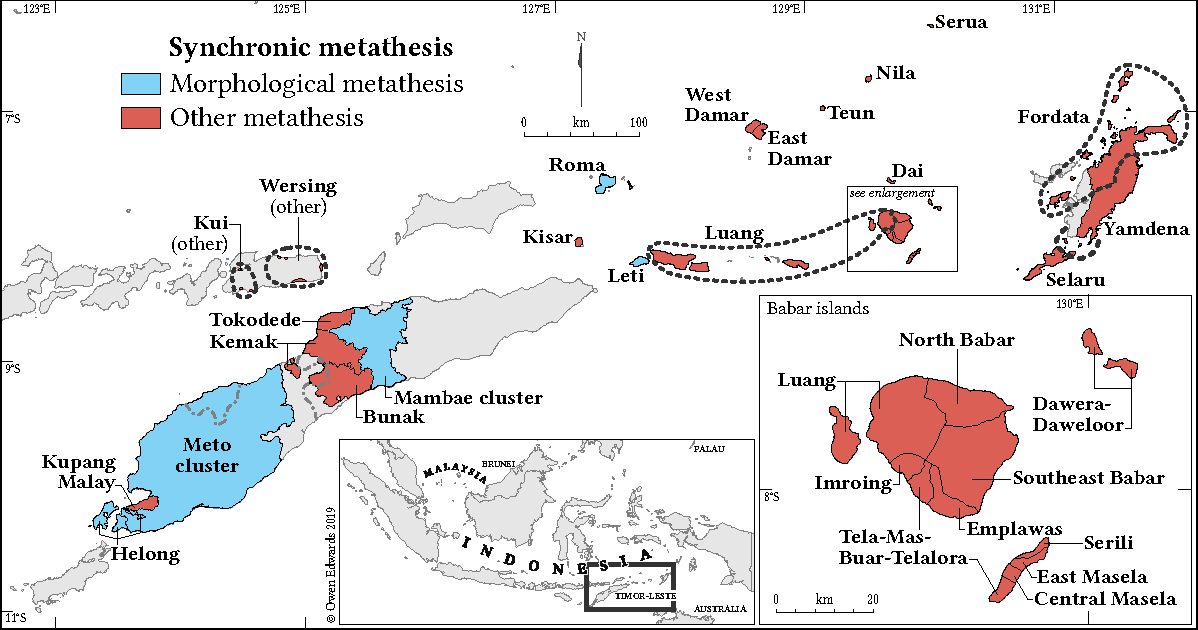
\includegraphics[width=\columnwidth]{SynchronicMetathesis.pdf}
\end{figure}

A map of languages in the greater Timor region
with synchronic metathesis is given in \frf{fig:CVMetTimReg},
based on \citet[135ff]{sc15}, a survey of the literature,
and my own fieldwork.
This map further marks languages in which metathesis
is known to be morphological in at least some environments.
\emph{Other metathesis} in \frf{fig:CVMetTimReg} is used for languages
with phonologically or morphemically conditioned metathesis,
as well as for languages for which too little data is available
to determine the nature of their metathesis.

There are at least five languages of the greater Timor region
with morphological metathesis in at least some environments:
Leti (\srf{sec:Let}), Roma (\srf{sec:Rom}), Mambae (\srf{sec:Mam}),
Helong (\srf{sec:Hel}) and the Meto cluster (of which Amarasi is a member).
A further twenty or so languages have synchronic
metathesis which is phonologically conditioned,
morphemically conditioned or not yet unambiguously established as morphological.

I begin my discussion with Kwara'ae (\srf{sec:Kwa})
and Rotuman (\srf{sec:Rot}), both of which are spoken in the Pacific
and outside the greater Timor region.
I then discuss cases of synchronic metathesis
in the greater Timor region starting with the non-Austronesian
languages Wersing (\srf{sec:Wer}) and Bunak (\srf{sec:Bun}).
After this I discuss synchronic metathesis among Austronesian
languages of the greater Timor region moving geographically
closer to Meto with each language discussed.

Before proceeding with the discussion
it is necessary to clarify two points.
Firstly, in some cases I give isolated examples of metathesis
of the type X {\ra} Y
(e.g. Rotuman \it{ho\tbr{sa}} {\ra} \it{ho\tbr{as}}
`flower' on page \pageref{ex:VCV->VVC})
or X + Z {\ra} YZ (e.g. Luang \it{ʔer\tbr{nu}} + \it{la}
{\ra} \it{ʔer\tbr{un}la} `go down to' on page \pageref{ex:LuaMet}).
In all such cases the form before the arrow is
a form which surfaces in certain contexts.
Thus, all putative examples of metathesis throughout this section
are based on true surface alternations.\footnote{
		Readers who find a particular analysis involving metathesis
		unconvincing should consult the original sources for full
		discussion and justification.}

Secondly, in such examples the form
before the arrow is the presumed underlying form.
The identification of underlying forms follows that of the sources,
which in turn is usually based on phonological and morphological analysis.
However, I do not usually repeat here the evidence for this analysis.
Interested readers should consult the original sources.
Again, in all cases the presumed underlying form
is a form which surfaces in certain contexts, as discussed above.
	\subsection{Kwara'ae}\label{sec:Kwa}
Metathesis in Kwara'ae has been described by
\citet{so80} and \citet{he04,he05}.
\citet{blga98} also present previously unpublished data
collected by Andrew Pawley and David Gegeo.
Metathesis in Kwara'ae has been analysed as phonologically conditioned (\srf{sec:PhoMet})
but it is not restricted to a subset of words with specific phonological properties.
Instead nearly every word of the lexicon is affected by metathesis in Kwara'ae.

\subsubsection{Forms}
Metathesis in Kwara'ae is CV {\ra} VC metathesis.
Examples are shown in \qf{ex:KwVCV->VVC} below.
In the literature on Kwara'ae the unmetathesised
form (U\=/form) is called the \emph{citation form} and the metathesised form
(M\=/form) is called the \emph{normal form}.
I refer to them with the more iconic terms \emph{U\=/form} and \emph{M\=/form}.

\begin{exe}
	\ex{V\sub{1}CV\sub{2} {\ra} V\sub{1}V\sub{2}C \hfill\citep[1]{he04}}\label{ex:KwVCV->VVC}
	\sn{\gw\begin{tabular}{rcll}
		 U\=/form 					&			& \mc{2}{l}{M\=/form}  \\
		\it{ˈlo.\tbr{ʔi}} &{\ra}& \it{ˈlo\tbr{i̯ʔ}} & `snake' \\
		\it{ˈbu.\tbr{ri}} &{\ra}& \it{ˈbu̯\tbr{ir}} & `behind' \\
		\it{ˈbo.\tbr{re}} &{\ra}& \it{ˈbo̯\tbr{er}} & `although' \\
	\end{tabular}}
\end{exe}

Depending on the length of the word,
metathesis in Kwara'ae can occur multiple times.
Two examples are given in \qf{ex:MulMetKwa} below.
The difference in stress which is seen in examples such as
\it{da.ˈro.ʔa.ˌni.da} {\ra} \it{ˈdao̯r.ʔa.ˌni̯ɛd} `to share them'
is significant and is the phonological conditioning environment
by which \cite{he04} analyses Kwara'ae metathesis.

\begin{exe}
	\ex{Kwara'ae multiple metatheses: \hfill\citep[2]{he04}}\label{ex:MulMetKwa}
	\sn{\gw\begin{tabular}{rcll}
		 U\=/form														&			& M\=/form &  \\
		\it{ˈke.\tbr{ta}.ˌla.\tbr{ku}} 	&{\ra}& \it{ˈke̯\tbr{at}.ˌla\tbr{u̯k}} & `my height' \\
		\it{da.ˈ\tbr{ro}.ʔa.ˌni.\tbr{da}}&{\ra}& \it{ˈda\tbr{o̯r}.ʔa.ˌni̯\tbr{ɛd}} & `to share them' \\
	\end{tabular}}
\end{exe}

Metathesis in Kwara'ae often triggers other phonological processes
including glide formation, vowel deletion, and umlaut.
The different phonological processes with which metathesis
is associated are described in \srf{sec:KwaGliFor}--\srf{sec:KwaSum} below.

Published descriptions of Kwara'ae report different
details for some of these phonological processes.
In part these differences may stem from researchers working
with different speakers of different ages.
However, another likely source of variation
is that a single speaker can also use
different M\=/forms depending on speech speed
(Patrick Andrews p.c. February 2015).

In addition to the difference in metathesis,
U\=/forms have the labiodental fricative [f]
where M\=/forms have the voiceless glottal fricative [h] \citep[18]{he04}.

\paragraph{Glide formation}\label{sec:KwaGliFor}
As can be seen from the examples in \qf{ex:KwVCV->VVC} and \qf{ex:MulMetKwa},
when a vowel sequence surfaces in the M\=/form,
the higher vowel is realised as a glide. %\citep[22]{he04}.
If the vowels are of equal height,
as in \it{ˈbo.re} {\ra} \it{ˈbo̯er} `although',
the first vowel is realised as a glide.
\citet[319]{so80} likewise states that metathesised forms consist only of one syllable,
though he does not give rules for which of the underlying vowels surfaces as a glide.

When a word ends in a vowel sequence,
the M\=/form is derived from the U\=/form through glide formation alone.
This is shown in \qf{KwaVV} below:

\begin{exe}
\ex{V\sub{1}V\sub{2} {\ra} V̯\sub{1}V\sub{2}\hfill\citep[13]{he04}}\label{KwaVV}
	\sn{\gw\begin{tabular}{rcll}
		 U\=/form								&			& M\=/form &  \\
		\it{ʔo.ˈd\tbr{o.a}} 	&{\ra}& \it{ˈʔo.d\tbr{o̯a}} & `wall' \\
		\it{ˈd\tbr{o.e}} 			&{\ra}& \it{ˈd\tbr{o̯e}} & `great, big' \\
		\it{ˈne.i.ˌr\tbr{i.a}}&{\ra}& \it{ˈnei̯.ˌr\tbr{i̯ɛ}} & `this one' \\
	\end{tabular}}%
\end{exe}

\paragraph{Vowel deletion}
When a word ends in V\sub{1}V\sub{2}CV\sub{3}{\#},
and V\sub{2} and V\sub{3} are of the same quality,
the first two vowels undergo glide formation and
the final vowel is deleted.
This is shown in \qf{KwaVseq1} below.

\begin{exe}
	\ex{V\sub{1}{\sub{α}}V\sub{2}{\sub{β}}CV\sub{3}{\sub{β}} {\ra} V̯\sub{1}{\sub{α}}V\sub{2}{\sub{β}}C \hfill\citep[27-28]{he04}}\label{KwaVseq1}
	\sn{\gw\begin{tabular}{rcll}
			U\=/form							&			& M\=/form &  \\
			\it{fu.ˈi.r\tbr{i}} &{\ra}& \it{ˈhu̯ir} & `that' \\
			\it{bi.ˈa.l\tbr{a}} &{\ra}& \it{ˈbi̯al} & `smoke' \\
	\end{tabular}}%
\end{exe}

\paragraph{Vowel shift}\label{sec:KwaVoShi}
The low central vowel /a/ has a different quality
after metathesis when the preceding vowel is high.
It is described as schwa [ə] by \citet[315]{so80},
while \citet[23]{he04} describes it as varying between
[ɛ] and [ə] after /i/ and as [ʌ] after /u/.
Examples are given in \qf{Kw2} below.

\begin{exe}
	\ex{V\tsc{[+hi]}Ca {\ra} V̯əC: \hfill\citep[23]{he04}}\label{Kw2}
		\sn{\gw\begin{tabular}{rcll}
			 	U\=/form								&			& M\=/form &  \\
				\it{a.ˈsi.\tbr{la}} 	&{\ra}& \it{ˈa.ˌsi̯\tbr{ɛl} {\tl} ˈa.ˌsi̯\tbr{əl}} & `sweet' \\
				\it{fa.ˈʔu.\tbr{ta}}	&{\ra}& \it{ˈha.ˌʔu̯\tbr{ʌt}} & `which, how, why' \\
		\end{tabular}}
\end{exe}

Likewise, certain combinations of vowel ``fuse'' into
a single vowel rather than a sequence of glide and vowel.
\citet[316]{so80} gives a rule in which /oi/ is realised as [øˑ],
/oe/ as [œˑ], /ae/ as [æˑ] and /ai/ is realised as either [ɛi] or [ɛˑ].
This is similar to the processes of umlaut which have
operated in the Germanic languages (\srf{sec:OriUml}).


\begin{exe}
	\ex{V\sub{α}CV\sub{β} {\ra} V\sub{αβ}C \hfill\citep[316]{so80}}\label{KwVfusionS}
		\sn{\gw\begin{tabular}{rcll}
			 U\=/form														&			& M\=/form &  \\
			\it{m\tbr{o}l\tbr{i}} 						&{\ra}& \it{m\tbr{øˑ}l} 							& `lemon' \\
			\it{as\tbr{o}f\tbr{e}} 						&{\ra}& \it{as\tbr{œˑ}f} 						& `rat' \\
			\it{m\tbr{a}ʔ\tbr{e}t\tbr{a}ʔ\tbr{e}elo}&{\ra}& \it{m\tbr{æˑ}ʔ.t\tbr{æˑ}ʔ.eol} & `doorway' \\
			\it{d\tbr{a}m\tbr{i}} 						&{\ra}& \it{d\tbr{ɛi}m {\tl} d\tbr{ɛˑ}m}	& `gum' \\
		\end{tabular}}
\end{exe}

\citet{he04} does not report front rounded vowels,
but he does report a similar process when the first vowel of the sequence is /a/.
He states that ``[{\ldots}] there is some free variation: if V\sub{2} = [e], [i] or [u],
sometimes the vowel combination can be realized as a single vowel.''
He only gives examples of /ae/ {\ra} [æˑ], /ai/ {\ra} [eˑ] and /au/ {\ra} [oˑ].

\begin{exe}
	\ex{V\sub{α}CV\sub{β} {\ra} V\sub{αβ}C \hfill\citep[24]{he04}}\label{KwVfusionH}
		\sn{\gw\begin{tabular}{rcll}
			 U\=/form										&			& M\=/form &  \\
			\it{ˈs\tbr{a}.t\tbr{e}}		&{\ra}& \it{ˈs\tbr{æ}ˑt} {\tl} \it{ˈs\tbr{ae̯}t} & `chin, beard' \\
			\it{ˈm\tbr{a}.ʔ\tbr{i}}		&{\ra}& \it{ˈm\tbr{eˑ}ʔ} {\tl} \it{ˈm\tbr{ai̯}ʔ} & `come' \\
			\it{li.ˈm\tbr{a}.k\tbr{u}}&{\ra}& \it{ˈli.ˌm\tbr{oˑ}k} {\tl} \it{ˈli.m\tbr{au̯}k} & `my hand' \\
		\end{tabular}}%
\end{exe}

\paragraph{Long vowels}\label{sec:KwaLonVow}
When the penultimate and final vowel of the U\=/form are identical,
\citet{so80}, Pawley and Gegeo (cited in \citealt{blga98}) and \citet{he04}
all transcribe the vowel of the M\=/form as half-long, using the symbol [ˑ].
Other descriptions of Kwara'ae, such as,
\citet{si77} and \citet{trha83} do not transcribe such vowels as long.

\begin{exe}
	\ex{V\sub{α}CV\sub{α} {\ra} V\sub{α}ˑC \hfill\citep[25]{he04}}\label{KwlongV}
		\sn{\gw\begin{tabular}{rcll}
			 U\=/form									&			& M\=/form &  \\
			\it{ˈk\tbr{i}.n\tbr{i}} &{\ra}& \it{ˈk\tbr{iˑ}n} & `female' \\
			\it{ˈm\tbr{a}.n\tbr{a}} &{\ra}& \it{ˈm\tbr{aˑ}n} & `her/his eye' \\
			\it{ˈm\tbr{o}.k\tbr{o}} &{\ra}& \it{ˈm\tbr{ɔˑ}k} & `smell' \\
		\end{tabular}}
\end{exe}

However, as noted by \citet[25]{he04},
no author justifies the use of this half-long mark,
with \citeauthor{he04} indicating that this is a point for further research.
An instrumental phonetic study of Kwara'ae vowels
would probably settle the matter.\footnote{
		For Amarasi I carried out an instrumental study of vowel length
		in which I showed that there is a statistically significant
		difference in length between the penultimate vowel of a U\=/form
		with identical penultimate and final vowels and the final
		vowel of the M\=/form of such words.
		I analyse this difference in length as being due to the M\=/forms
		containing a sequence of two identical vowels.
		(see \srf{sec:QuaLenVowSeq} and \srf{sec:QuaMfoEndVVC}).}
It is also possible that such vowels are long in some contexts and short in others,
depending on variables such as phrasal stress and the rate of speech.

\paragraph{Voiceless vowels}\label{sec:KwaVoiVow}
Optional voiceless vowels also occur after certain consonants in the U\=/form.
\citet[19]{he04} reports such vowels after the consonants [ʔ], [h], [l] and [s].
These vowels do not count as vowels for the purposes of stress assignment,
with stress falling on the penultimate vowel, not counting final voiceless vowels.
After word-final stops, voiceless vowels do not occur,
though the final stop is often strongly aspirated.

\begin{exe}
	\ex{V\sub{1}CV\sub{2} {\ra} V\sub{1}V\sub{2}C{\r*V}\sub{2} \hfill\citep[19]{he04}}\label{KwvoicelessVH}
		\sn{\gw\begin{tabular}{rcll}
			 U\=/form			&			& M\=/form &  \\
			\it{ˈma.ʔu} &{\ra}& \it{ˈmau̯ʔ\tbr{u̥}} & `fear' \\
			\it{ˈʔa.fe} &{\ra}& \it{ˈʔae̯h\tbr{e̥}} & `wife' \\
			\it{ˈbu.su} &{\ra}& \it{ˈbuˑs\tbr{u̥}} & `to burst' \\
			\it{ˈro.do} &{\ra}& \it{ˈrɔˑ\tbr{dʰ}} & `night' \\
			\it{ˈnau̯.ku} &{\ra}& \it{ˈnau̯\tbr{kʰ}} & `I' \\
		\end{tabular}}
\end{exe}

Pawley and Gegeo (cited in \citealt{blga98})
describe voiceless vowels in a wider variety of contexts than is described by \citet{he04}.
According to Pawley and Gegeo, a final voiceless vowel is the usual realisation of words in the M\=/form.
Such vowels only do not occur when there is a word-final nasal
or if the resulting diphthong is a sequence of a high vowel followed by a non-high vowel.

\begin{exe}
	\ex{V\sub{1}CV\sub{2} {\ra} V\sub{1}V\sub{2}C{V̥}\sub{2} \hfill(Pawley and Gegeo in \citealt[530]{blga98})}\label{KwvoicelessVBG}
		\sn{\gw\begin{tabular}{rcll}
			 U\=/form			&			& M\=/form &  \\
			\it{ˈfusi}	&{\ra}& \it{huis\tbr{i̥}} & `cat' \\
			\it{ˈkado}	&{\ra}& \it{kaod\tbr{o̥}} & `thin' \\
			\it{ˈoso}		&{\ra}& \it{oˑs\tbr{o̥}} & `lie' \\
	\end{tabular}}
\end{exe}

According to \citet[20]{he04},
the differences between his data and the data cited by \citet{blga98}
likely comes from working with speakers of different generations.
\citeauthor{he04} states: \emph``[{\ldots}] it's reasonable that her [Kwara'ae consultant's]
speech pattern reflects another stage in the decline of the final vowel.''
%The aspiration of final stops reported by \citet[18]{he04} seems also to
%represent the final remnant of the voiceless vowels reported by Pawley and Gegeo.

\begin{table}[h]
	\caption{Kwara'ae metathesis}\label{tab:KwaMet}
	\begin{tabular}{c|ccccccl}
		\lsptoprule
	V\sub{1}{\da}	&i							&e						&a				&o	&u			&	{\la}V\sub{2}\\			
			\midrule
			i	&{iˑ}										&--						&jɛ, jə		&jo	&ju			&\\
			e	&{ej}										&ɛˑ						&e̯a				&e̯o	&ew			&\\
			a	&{aj, ej, eˑ, (ɛj, ɛˑ)}	&{æ;, ae̯}			&aˑ				&ao̯	&aw, oˑ	&\\
			o	&{oj, (øˑ)}							&o̯e, we, (œˑ)	&o̯a				&ɔˑ	&ow			&\\
			u	&{wi}										&wɛ						&wʌ, (wə)	&--	&uˑ			&\\
		\lspbottomrule
	\end{tabular}
\end{table}

\paragraph{Summary}\label{sec:KwaSum}
The processes with which metathesis in Kwara'ae is associated
include glide formation, umlaut, and vowel deletion.
The effects of deriving the M\=/form on the first
and second vowels of the U\=/form in Kwara'ae are given in \trf{tab:KwaMet}.
This table is adapted from \citep[26]{he04} with qualities reported by \citet{so80} included in brackets.
The symbols used by \citeauthor{he04} for the high vowel glides:
[u̯] and [i̯], have been replaced with the symbols [w] and [j].

\subsubsection{Distribution of metathesis}\label{sec:KwaFun}
U\=/forms and M\=/forms in Kwara'ae belong to different speech registers.
In everyday normal speech the M\=/form is used,
while the U\=/form is used in traditional songs,
for clarification \citep[3]{he04}, and when calling out.
\citet[19]{wage86} report that calling out has three main uses in Kwara'ae discourse:

\begin{quote}
First, people call out for practical reasons in running a household,
such as to locate a missing person or to bring a family member home for a meal.
Secondly, a Kwara'ae man or woman working in the bush and hearing someone
working nearby but out of sight will call out to seek identification of the other person.
Thirdly, people call out from house to house, or as someone passes on the path, as a strictly social activity.
They ask polite questions, or joke, tease, and engage in pleasant banter. \hfill\citep{wage86}
\end{quote}

In addition to the use of unmetathesised forms, calling out is marked
by a special intonation contour and certain emphatic particles.
Two examples of Kwara'ae calling out are given in \qf{KwCallingOut} below.
Note also the extra length on the final syllable of the second form of `father' in example
\qf{KwCallingOut1} as well as the particle \emph{ku} in \qf{KwCallingOut2}.
These two features are also distinctive of calling out.

\begin{exe}\let\eachwordone=\itshape
	\ex{Kwara'ae calling out: \hfill\citep[24,21]{wage86}}\label{KwCallingOut}
		\begin{xlist}
			\ex{
				\gll maʔ! ma\tbr{ʔaːː}! \\
				father{\textbackslash}\tsc{m} father{\tbrU} \\
				\glt `Dad! Da-ad!'\label{KwCallingOut1}}
			\ex{
				\gll Sa\tbr{la}! Sal! Sal ku! lae maiʔ tua hain Mo\tbr{sa}! \\
				Sala{\tbrU} Sala{\M} Sala{\M} \tsc{part} go here stay with:\tsc{3sg.poss} Mosa{\tbrU} \\
				\glt `Sala! Sala! Hey, Sala! Come here and babysit Mosa!' \label{KwCallingOut2}}
		\end{xlist}
\end{exe}

The use of different forms in different speech registers is confirmed by Patrick Andrews
(p.c. February 2015)
who reports that (among other uses) the unmetathesised forms
are used when making a point to a child or to emphasise words in a speech.
He compares the use of the metathesised forms to that of English contractions,
such as \it{couldn't} from \it{could not},
with the former being the everyday form and the latter being used in special circumstances.
This difference in distribution suggests that different forms
are used in different (discourse) pragmatic contexts.

\cite{he04} proposes an analysis of Kwara'ae metathesis framed within Optimality Theory
in which metathesis is conditioned by stress.
Under this analysis, metathesis in Kwara'ae is a response
to the need to make stressed syllables heavy,
with a vowel-glide combination counting as a heavy syllable.
This analysis is discussed in more detail in \srf{sec:ProMorKwa}.

Given that different forms are used in different speech registers,
an analysis of Kwara'ae metathesis as being driven by stress
would predict that different registers have different stress rules.
While it is likely that such a hypothesis would be borne out,
to the best of my knowledge this has not yet been demonstrated.

Nearly every word in Kwara'ae is affected by metathesis.
If it is the case that different speech registers have
different stress patterns, which in turn drives the metathesis,
Kwara'ae has (rampant) phonologically conditioned metathesis
though the phonological conditions triggering metathesis
are themselves driven by the discourse.

	\subsection{Rotuman}\label{sec:Rot}
\il{Rotuman|(}Rotuman has perhaps the most famous case of morphological metathesis.
Rotuman is an Austronesian Oceanic language spoken on Rotuma island
in the Pacific Ocean located about 480 kilometres north of the main islands of Fiji.
Metathesis occurs in multiple environments in Rotuman,
discussed in fuller detail in \srf{sec:RotFun}
In some cases metathesis is phonologically conditioned (\srf{sec:PhoMet}),
in some cases it is morphemically conditioned (\srf{sec:MorpheConMet}),
and in some cases it is morphological (\srf{sec:MorMet}).

Rotuman was first described by \citet{ch40} which is a grammar and dictionary of the language.
\citeauthor{ch39} also published several Rotuman texts between 1937--39 in the journal \it{Oceania}
which were reprinted in one volume as \citet{ch39}.
Both \citet{be87} and \citet{va02} also present descriptions of
Rotuman based on their own fieldwork.
Each of these descriptions differs in details.
This may be partly because the authors worked with different
speakers at different times and may also be partly because they use
different terminology to describe the same phenomena.

\subsubsection{Forms}\label{sec:RotFor}
Each word in Rotuman has two forms, which I call the the U-form and M-form.
The traditional names coined by \cite{ch40} are the \it{complete phase} for the U-form
and the \it{incomplete phase} for the M-form.
The U-form is historically more conservative than the M-form.

\cite{ch40} identifies four phonological processes
which derive the M-form from the U-form.
These processes are vowel deletion (a.k.a apocope, truncation or subtraction),
umlaut, metathesis and vowel shortening.
There are also words which do not have two distinct forms.
Which process applies depends on the phonological shape of the U-form.
%Examples are given in \qf{ex:RotLonShoChu} below,
%and discussed in more detail in \srf{sec:RotDip}--\srf{sec:RotSum}.

%\begin{exe}
%	\ex{Rotuman U-forms and M-forms \hfill\citep[85]{ch40}}\label{ex:RotLonShoChu}
%		\sn{\begin{tabular}{llll}
%			U-form&M-form	&						&Process \\
%			\it{mata}	&\it{mat}			&`wet'			&apocope \\
%			\it{mose}	&\it{mœs}			&`to sleep'	&umlaut	\\
%			\it{toka}	&\it{toak}		&`to cease'	&metathesis\\
%			\it{ʧao}	&\it{ʧ\u{a}o}	&`spear'		&V shortening \\
%			\it{rii}	&\it{rii}			&`house'		&n./a. \\
%		\end{tabular}}
%\end{exe}

\paragraph{Vowel shortening/diphthongisation}\label{sec:RotDip}
For words which end in a sequence of non-identical vowels,
\cite[85]{ch40} describes the M-form as being formed
by shortening the initial vowel of the sequence.
Examples are given in \qf{VV->VV-Chu} below.

\begin{exe}
	\ex{Rotuman V{\sub{α}}V{\sub{β}} {\ra} \u{V}{\sub{α}}V{\sub{β}} \hfill\citep[85]{ch40}}\label{VV->VV-Chu}
	\sn{\gw\begin{tabular}{lcll}
			U-form		&		&M-form			&\\
		\it{pupui}	&\ra& \it{pup\u{u}i}	& `floor' \\
		\it{ʔesʔao} &\ra& \it{ʔesʔ\u{a}o} & `useful' \\
		\it{lelei}	&\ra& \it{lel\u{e}i}	& `good' \\
		\it{foʔou}	&\ra& \it{foʔ\u{o}u}	& `new' \\
	\end{tabular}}
\end{exe}

\cite{va02} describes a process of diphthongisation
in which the less sonorous vowel becomes a glide.
This glide formation may be either a further development 
of \citeauthor{ch40}'s shortened vowels, or it may that
a single phenomenon was perceived and described differently
by each of these authors.

\begin{exe}
	\ex{Rotuman V{\sub{α}}V{\sub{β}} {\ra} V̯{\sub{α}}V{\sub{β}} {\tl} V{\sub{α}}V̯{\sub{β}}
	\hfill\citet[4,7--9]{va02}}\label{VV->VV-Vam}
		\sn{\gw\begin{tabular}{lcll}
			U-form			&		&	M-form		&\\
			\it{lio}		&\ra& \it{ljo}	& `voice' \\
			\it{fau}		&\ra& \it{faw}	& `year' \\
			\it{fui}		&\ra& \it{fuj}	& `piece of garland' \\
			\it{fɒi}		&\ra& \it{fɒj}	& `chop down' \\
			\it{momoe}	&\ra& \it{momoe̯} & `k.o. tree' \\
		\end{tabular}}
\end{exe}

According to \citet[210]{be87} the vowel sequences which
diphthongise are those in which the second vowel is /a/
as well as sequences of a high vowel followed by /o/.
\citeauthor{be87} also reports that /a/
is realised as [ɔ] after a glide derived
from one of the high-front vowels.

\begin{exe}
	\ex{Rotuman V{\sub{α}}V{\sub{β}} {\ra} V̯{\sub{α}}V{\sub{β}} \hfill\citep[210]{be87}}\label{RotDip-be}
	\sn{\gw\begin{tabular}{lcll}
			U-form	&		&	M-form		&\\
		\it{ʔea}	&\ra& \it{ʔja}	& `to say' \\
		\it{foa}	&\ra& \it{fwa}	& `coconut scraper' \\
		\it{kia}	&\ra& \it{kjɔ}	& `neck' \\
		\it{sua}	&\ra& \it{swɔ}	& `shoot (of a plant)' \\
	\end{tabular}}
\end{exe}

\paragraph{Metathesis}\label{sec:RotMet}
When the U-form ends in VCV and the penultimate vowel is higher than the final vowel,
the M-form is derived by final consonant-vowel metathesis.
Examples are given in \qf{ex:VCV->VVC} below.

\begin{exe}
	\ex{Rotuman V\sub{1}CV\sub{2} {\ra} V\sub{1}V\sub{2}C \hfill\citep[14]{ch40}}\label{ex:VCV->VVC}
		\sn{\gw\begin{tabular}{lcll}
			U-form					&		&M-form&\\
			\it{pu\tbr{re}} &\ra& \it{pu\tbr{er}} & `to rule, decide' \\
			\it{ho\tbr{sa}} &\ra& \it{ho\tbr{as}} & `flower' \\
			\it{ti\tbr{ko}} &\ra& \it{ti\tbr{ok}} & `flesh' \\
			\it{pe\tbr{pa}} &\ra& \it{pe\tbr{ap}} & `paper' \\
		\end{tabular}}
\end{exe}

Both \citet{va02} and \citet{be87} report that after metathesis
the penultimate vowel becomes a glide;
/u/ and /o/ become [w] while /i/ and /e/ become [j].
Examples are given in \qf{ex:VCV->VVC-Vam} below.

\begin{exe}
	\ex{Rotuman V\sub{1}CV\sub{2} {\ra} V̯\sub{1}V\sub{2}C \hfill\citep[3]{va02}}\label{ex:VCV->VVC-Vam}
	\sn{\gw\begin{tabular}{lcll}
			U-form				&		&	M-form&\\
		\it{pu\tbr{re}} &\ra& \it{pw\tbr{ɛr}} & `rule' \\
		\it{fu\tbr{pa}} &\ra& \it{fw\tbr{ap}} & `to distribute' \\
		\it{ʔi\tbr{ko}} &\ra& \it{ʔj\tbr{ɔk}} & `thrust' \\
	\end{tabular}}
\end{exe}

\citet[208]{be87} reports that when the penultimate vowel is a high vowel,
the final vowel becomes [ɔ] after metathesis.
Otherwise, the final vowel retains its original quality.
Examples are given in \qf{ex:VCV->VVC-Bes} below.

\begin{exe}
	\ex{Rotuman V\sub{1}CV\sub{2} {\ra} V̯\sub{1}V\sub{2}C \hfill\citep[208]{be87}}\label{ex:VCV->VVC-Bes}
	\sn{\gw\begin{tabular}{lcll}
			U-form				&		&	M-form&\\
		\it{ti\tbr{fe}}	&\ra& \it{tj\tbr{ɔf}} & `pearl shell' \\
		\it{pi\tbr{ʧa}} &\ra& \it{pj\tbr{ɔʧ}} & `rat' \\
		\it{hu\tbr{ŋe}}	&\ra& \it{hw\tbr{ɔŋ}} & `to breathe' \\
		\it{pu\tbr{ka}}	&\ra& \it{pw\tbr{ɔk}} & `k.o. creeper' \\
		\it{he\tbr{pa}}	&\ra& \it{hj\tbr{ap}} & `broad' \\
		\it{lo\tbr{ŋa}}	&\ra& \it{lw\tbr{aŋ}} & `towards the interior of the island' \\
	\end{tabular}}
\end{exe}

It is not entirely clear whether the diphthongisation
after metathesis reported by \cite{be87} and \cite{va02}
is a recent development or whether it was also present
while \citeauthor{ch40} worked on Rotuman.

On the one hand, it is clear from the detailed account of
Rotuman phonetics given by \citet[64--84]{ch40},
that he was an excellent phonetician.
Given his identification of shortened vowels
in the derivation of M-forms (\srf{sec:RotDip}),
it seems likely that if diphthongisation (or shortened vowels)
were present after metathesis he would have reported it.

On the other hand, \citet[86]{ch40} states
``[T]he stress seems to be levelled out, so
to speak, in the inc[omplete] phase.
Thus: \it{fo}ra becomes \it{foar}, which is pronounced almost,
though perhaps not quite, as one syllable,
the stress being evenly distributed [\ldots]''
This statement perhaps indicates that diphthongisation
was an optional feature of Rotuman metathesised
forms in \citeauthor{ch40}'s day.

\paragraph{Umlaut}\label{sec:RotUml}
When the penultimate vowel is a back vowel and the final vowel a front vowel,
the M-form is derived via umlaut of the penultimate vowel
so long as this vowel is not higher than the final vowel.

\citet[79]{ch40} reports that /u/ becomes [y],
/o/ becomes [œ] when the final vowel is /e/,
and that /o/ becomes [ø] when the final vowel is /i/.\footnote{
	\cite{ch40} describes the vowel in the M-form of oCe{\#} final words
	(e.g. \it{mose} {\ra} \it{mœs} `sleep')
	as ``[\ldots] similar to the wider German \it{ö}, as in \it{gespött},
	and to the sound of \it{eu} in the French \it{jeune}.''
	He contrasts `normal \it{ö}' (which ``[\ldots] arises in place of normal \it{o} when a following \it{e} is elided'')
	with so-called `narrow \it{ö}' (arising ``[\ldots] in place of narrow \it{o} when a following \it{i} is elided'')
	which is described as ``[\ldots] similar to the narrower German \it{ö}, as in \it{schön},
	and to the sound of \it{eu} in the French \it{peu}.''
	I interpret `normal \it{ö}' as a mid-low front-rounded vowel [œ]
	and `narrow \it{ö}' as a mid-high front-rounded vowel [ø].}
He also transcribes the outcome of umlauted /ɒ/ as \it{<\.a>},
describing it as ``[\ldots] a little wider [lower] than \it{a} in `cat' [\ldots]
but differs from it in containing just a suggestion of the sound of \it{u} in `cut' or `but.'{''}
In interpret \citeauthor{ch40}'s \it{<\.a>} as a low front rounded vowel [ɶ].

Examples of Rotuman umlaut are given in \qf{RotUml-ch} below,
which also gives hypothetical intermediate forms
showing the way such umlaut probably developed from metathesis.
In Kwara'ae (\srf{sec:KwaVoShi}) words containing some of the vowel combinations
shown in \qf{RotUml-ch} have M-forms which vary between displaying metathesis and umlaut.

\begin{exe}
\ex{V\tsc{[+rnd]}CV\tsc{[+fr]} {\ra} V\tsc{[+rnd,+fr]}C \hfill\citep[79-80]{ch40}}\label{RotUml-ch}
	\sn{\gw\begin{tabular}{lclcll}
			U-form	& &						& &	M-form&\\
		\it{ʔuli} &>&\it{*ʔuil}	&>& \it{ʔyl} & `skin' \\
		\it{mori} &>&\it{*moir}	&>& \it{mør} & `orange (fruit)'	 \\
		\it{mose} &>&\it{*moes}	&>& \it{mœs} & `to sleep' \\
		\it{ʔɒfi} &>&\it{*ʔɒif}	&>& \it{ʔɶf} & `to bite' \\
	\end{tabular}}
\end{exe}

\citet{va02} reports that /o/ becomes [ø] under umlaut,
/u/ becomes [y] and /ɒ/ becomes the lower mid-front-rounded [œ].
Examples are given in \qf{RotUml-va}

\begin{exe}
\ex{Rotuman V\tsc{[+ba]}CV\tsc{[+fr]} {\ra} V\tsc{[+fr]}C \hfill\citep[3]{va02}}\label{RotUml-va}
	\sn{\gw\begin{tabular}{lcll}
			U-form	&		&	M-form&\\
		\it{futi} &\ra& \it{fyt} & `to pull' \\
		\it{mose} &\ra& \it{møs} & `to sleep' \\
		\it{pɒri} &\ra& \it{pœri} & `banana' \\
	\end{tabular}}
\end{exe}

\citeauthor{be87}'s data agrees with \citeauthor{va02} on the outcome of /o/ and /u/,
though he reports that /ɔ/ (equivalent to \citeauthor{ch40}'s and \citeauthor{va02}'s /ɒ/)
becomes either [ɛ] or [æ] in free variation in certain words.
Examples are given in \qf{RotUml-be} below.

\begin{exe}
\ex{Rotuman V\tsc{[+ba]}CV\tsc{[+fr]} {\ra} V\tsc{[+fr]}C \hfill\citep[209]{be87}}\label{RotUml-be}
	\sn{\gw\begin{tabular}{lcll}
			U-form	&		&	M-form&\\
		\it{pɔti} &\ra& \it{pɛt} & `scar' \\
		\it{hɔʔi} &\ra& \it{hɛʔ} & `to pull' \\
		\it{pɔni} &\ra& \it{pɛn} & `paint' \\
	\end{tabular}}
\end{exe}

All authors agree that umlaut of /u/ or /o/ spreads leftwards to identical vowels.
Examples are given in \qf{RotUmlSpr} below

\begin{exe}
\ex{Rotuman umlaut spreading: \hfill\citep[79f]{ch40}}\label{RotUmlSpr}
	\sn{\gw\begin{tabular}{lcll}
			U-form			&\ra&	M-form&\\
		\it{furfuruki}&\ra& \it{fyrfyryk} & `pimple' \\
		\it{roromi} 	&\ra& \it{rørøm} & `unexpectedly' \\
		\it{popore} 	&\ra& \it{pœpœr} & `to dash, dart' \\
	\end{tabular}}%
\end{exe}

\paragraph{Apocope}\label{sec:RotApo}
In all situations not covered by diphthongisation, metathesis or umlaut,
the M-form is derived by deleting the final vowel of the U-form.
This includes when each vowel is identical and
when the penultimate vowel is lower than a final back vowel.
Examples are shown in \qf{ex:VCV->VC} below.

\begin{exe}
	\ex{Rotuman VCV {\ra} VC \hfill\citep[13]{ch40}}\label{ex:VCV->VC}
	\sn{\gw\begin{tabular}{lcll}
			U-form		&		&	M-form			&\\
		\it{haŋa}		&\ra& \it{haŋ}		& `to feed' \\
		\it{hɒŋu}		&\ra& \it{hɒŋ}		& `to awaken' \\
		\it{læʧe}	&\ra& \it{læʧ}		& `coral' \\
		\it{tokiri} &\ra& \it{tokir}	& `to roll' \\
		\it{hoto} 	&\ra& \it{hot}		& `to jump' \\
		\it{heleʔu} &\ra& \it{heleʔ}	& `to arrive' \\
	\end{tabular}}
\end{exe}

The lack of overt metathesis in such examples is comparable
to the Amarasi data in which words with a certain phonotactic
shape form their M-form by surface vowel deletion and/or consonant deletion (Chapter \ref{ch:StrMetAma}).

\paragraph{No change}
Words ending in two identical vowels
do not usually have distinct U-forms and M-forms according to \citet[85]{ch40},
except before certain suffixes in which case the final vowel of U-form is lengthened.
Examples are given in \qf{ex:VV->VV} below.

\begin{exe}
	\ex{Rotuman V{\sub{α}}V{\sub{α}} {\ra} V{\sub{α}}V{\sub{α}} \hfill\citep[85]{ch40}}\label{ex:VV->VV}
	\sn{\gw\begin{tabular}{lcll}
			U-form	&		&	M-form&\\
		\it{rii}	&\ra& \it{rii}	& `house' \\
		\it{ree}	&\ra& \it{ree}	& `to do' \\
%		\it{reeː-} & \it{ree-}	& `to do' \\
	\end{tabular}}
\end{exe}

\citet{be87} reports that when the sequence of two identical vowels is /aa/,
the M-form is formed by deleting the final vowel.
In other situations \citeauthor{be87} reports no difference in the two forms.
Examples are given in \qf{ex:aa->a} below.

\begin{exe}
	\ex{Rotuman /aa/ {\ra} /a/ \hfill\citep[212]{be87}}\label{ex:aa->a}
	\sn{\gw\begin{tabular}{lcll}
		 U-form		&		&	M-form&\\
		\it{ʔaa}	&\ra& \it{ʔa} & `bite' \\
		\it{ree}	&\ra& \it{ree} & `do' \\
		\it{luu}	&\ra& \it{luu} & `rope' \\
	\end{tabular}}%
\end{exe}

%This is consistent with \citeauthor{be87}'s account of diphthongisation in Rotuman.
%in which he reports that the only
%combinations of non-high vowels which diphthongise
%are those involving the vowel /a/
%(see example \qf{RotDip-be} \prf{RotDip-be}).

\paragraph{Summary of forms}\label{sec:RotSum}
The ways in which the Rotuman M-form is derived from the U-form
for CV{\#} final words are shown in \trf{tab:RotLonShoFor}.
In most cases the M-form is one syllable shorter than the U-form,
the main exceptions being word final sequences of identical vowels
and \citeauthor{ch40}'s metathesised forms.

\begin{table}[h]\stl{0.4em}
	\caption{Medial vowels of Rotuman U-forms and M-forms} \label{tab:RotLonShoFor}
		\begin{tabular}{r|ccccc|ccccc|ccccc|l}
		\lsptoprule
					&\mc{5}{c|}{\citet{ch40}}&\mc{5}{c|}{\citet{va02}}&\mc{4}{c}{\citet{be87}}\\
	V\sub{1}{\da}	&i	&e	&a	&o	&u	&i	&e	&a	&o	&u	&i	&e	&a	&o	&u	&{\la}V\sub{2}\\\midrule
							i	&i	&ie	&ia	&io	&i	&i	&jɛ	&ja	&jɔ	&i	&i	&jɔ	&jɔ	&jo	&i	&i\\
							e	&e	&e	&ea	&e	&e	&ɛ	&ɛ	&ja	&ɛ	&ɛ	&e	&e	&ja	&e	&e	&e\\
							a &ɶ	&æ	&a	&a	&ɒ	&œ	&æ	&a	&a	&ɒ	&ɛ	&ɛ	&a	&a	&ɔ	&a\\
							o	&ø	&œ	&oa	&o	&o	&ø	&ø	&wa	&ɔ	&ɔ	&ø	&ø	&wa	&o	&o	&o\\
							u	&y	&ue	&ua	&uo	&u	&y	&wɛ	&wa	&wɔ	&u	&y	&wɔ	&wɔ	&wo	&u	&u\\
		\lspbottomrule
	\end{tabular}
\end{table}

\subsubsection{Distribution of metathesis}\label{sec:RotFun}
Three uses of M-forms can be identified in Rotuman:
phonologically conditioned, morphemically conditioned, and morphological.
Each is discussed in turn.

\paragraph{Phonologically conditioned M-forms}\label{sec:RotPhoConMfo}
\citet{haki98} show that, with two exceptions,
the U-form is used before suffixes and enclitics
which are monosyllabic or non-syllabic,
while the M-form is used before polysyllabic suffixes and enclitics.

An example of the U-form before a monosyllabic suffix is given in \qf{RotUse1}
and an example before a non-syllabic suffix is given in \qf{RotUse2}.
An example of the M-form before a disyllabic affix is given in \qf{RotUse3}
and an example before a trisyllabic enclitic is given in \qf{RotUse4}.
These examples are taken from \cite[120f]{haki98}

\begin{exe}\let\eachwordone=\textit
	\ex{\gll	puʔa + ŋa {\ra} puʔa-ŋa \\
						{be greedy} {} \tsc{nmlz} {} greedy{\U}-\tsc{nmlz} \\
			\glt	`greed'}\label{RotUse1}
	\ex{\gll	vaka + t {\ra} vaka-t \\
						canoe {} \tsc{sg} {} canoe{\U}-\tsc{sg} \\
			\glt	`a canoe'}\label{RotUse2}
	\ex{\gll	furi + ʔian {\ra} fyr-ʔian \\
						turn {} \tsc{ingressive} {} turn{\M}-\tsc{ingressive} \\
			\glt	`start turning' }\label{RotUse3}
	\ex{\gll	vaka + teʔisi {\ra} vak=teʔisi \\
						canoe {} this {} canoe{\M}=this \\
			\glt	`this canoe' }\label{RotUse4}
\end{exe}

Similarly, each non-final word in the noun phrase occurs in the M-form.
That is, the M-form is used when a noun is modified;
it is used to mark the presence of a dependent modifier.
This is also a function of metathesis in Leti (\srf{sec:Let})
and Amarasi (Chapter \ref{ch:SynMet}).

Compare the phrases in \qf{ex:ThePeoAre} and \qf{ex:TheZeaPeo} below, from \citet[14]{ch40}.
Each phrase consists of the noun \it{famori} `people'
followed by the adjective \it{feʔeni} `zealous'.
In \qf{ex:ThePeoAre} the noun \it{famori} `people' is in the U-form
and the adjective has a predicative reading,
as illustrated in \qf{tr:ThePeoAre}.
In \qf{ex:TheZeaPeo} the noun \it{famør} `people' is in the M-form,
and the adjective has an attributive meaning,
as illustrated in \qf{tr:TheZeaPeo}.
(The use of the M-form of the adjective in \qf{ex:ThePeoAre}
and \qf{tr:ThePeoAre} is discussed in \srf{sec:RotMorMfo} below.)

\begin{multicols}{2}
	\begin{exe}\let\eachwordone=\it
		\ex{\gll fam\tbr{ori} feʔen\\
						people{\tbrU} zealous{\M}\\
				\glt `The people are zealous.'}\label{ex:ThePeoAre}
		\ex{\gll fam\tbr{ør} feʔeni\\
						people{\tbrM} zealous{\U}\\
				\glt `(The) zealous people.'}\label{ex:TheZeaPeo}
	\end{exe}
\end{multicols}
\begin{multicols}{2}
	\begin{exe}
		\ex{\begin{forest} where n children=0{tier=word}{}
			[S,[NP,[N,[\it{fam\tbr{ori}}\\people{\tbrU}]]][PRED,[\it{feʔen}\\zealous{\M}]]]
		\end{forest}}\label{tr:ThePeoAre}
		\ex{\begin{forest}
			[S,[NP,[N,[\it{fam\tbr{ør}}\\people{\tbrM}]][ADJ,[\it{feʔeni}\\zealous{\U}]]][{\ldots}]]
		\end{forest}}\label{tr:TheZeaPeo}
	\end{exe}
\end{multicols}

The generalisation identified by \citet{haki98}
is that the M-form is (mostly) used before polysyllabic modifiers,
while the U-form is used elsewhere.
This generalisation is the basis for the analysis
of \cite{mcc00} under the frameworks of prosodic
morphology and optimality theory.
This analysis is discussed in more detail in \srf{sec:ProMorRot}.

\paragraph{Morphemically conditioned M-forms}
As acknowledged by \citet{haki98},
there are two exceptions to their generalisation
that the M-form occurs before polysyllabic suffixes,
enclitics and modifiers.

The first exception is the monosyllabic singular marker \emph{-ta}.
Before this article M-forms occur, despite the fact that this suffix is monosyllabic.
An example of is given in \qf{RotUse6} below.

\begin{exe}
\let\eachwordone=\textit
	\ex{\gll mori + ta {\ra} m{\o}r-ta *mori-ta\\
		{orange} {} \tsc{sg} {} orange{\textbackslash}\tsc{m}-\tsc{sg} \\
		\glt `the orange' \hfill\citep[14]{va02}}\label{RotUse6}
\end{exe}

The second exception is that M-forms of nouns are used without any
affix/enclitic for a plural indefinite meaning,
while the U-form is used for a plural definite meaning.
Examples are given in \qf{ex:RotDef} and \qf{ex:RotInd}
from \citet[15]{ch40}

\begin{multicols}{2}
	\begin{exe}\let\eachwordone=\it
		\ex{\gll fam\tbr{ori} ʔea\\
						people{\tbrU} say\\
				\glt `The people say.'}\label{ex:RotDef}
		\ex{\gll fam\tbr{ør} ʔea\\
						people{\tbrM} say\\
				\glt `Some people say.' }\label{ex:RotInd}
	\end{exe}
\end{multicols}

\citet[121f]{haki98} analyse these exceptions by positing zero affixes with moraic weight.
Their analysis of the exceptional forms of \it{vaka/vak} `canoe'
is shown in \qf{ex:RotExcShoFor} below.\footnote{
	I cannot find a clear explanation in \cite{haki98} for why the noun \it{vaka}
	surfaces in the U-form when followed by the two suffixes
	{\0}\sub{PL} and {\0}\sub{DEF}.
	If I understand the analysis correctly,
	each null suffix should have moraic weight,
	with this combination of two suffixes being poly-moraic (polysyllabic)
	and thus triggering the M-form.}

\begin{exe}
\ex{Rotuman exceptional M-forms: \hfill\citep[122]{haki98}}\label{ex:RotExcShoFor}
	\sn{\gw\begin{tabular}{lll}
		\it{vaka} 	& /vaka + {\0}\sub{PL} + {\0}\sub{DEF}/ & `the canoes' \\
		\it{vak ta} & /vaka + ta + {\0}\sub{DEF}/ & `the one canoe' (i.e. `the canoe') \\
		\it{vaka-t} & /vaka + ta/ & `a/one canoe'\\
	\end{tabular}}
\end{exe}

An analysis involving multiple null suffixes with moraic weight
is not particularly convincing as an appropriate synchronic analysis of the Rotuman data.
Instead, given that U-forms are normally used before monosyllabic suffixes,
uses of the M-form before the singular suffix \it{-ta}
is better analysed as morphemically conditioned
and use of the M-forms to mark an indefinite plural is better
analysed as a morphological use of M-forms.

\paragraph{Morphological M-forms}\label{sec:RotMorMfo}
In addition to phonologically conditioned M-forms before polysyllabic modifiers
and morphemically conditioned M-forms before the singular suffix \it{-ta},
M-forms also occur as the only phonological realisation
of a semantic difference; morphological M-forms.
A number of different morphological uses of M-forms can be identified in Rotuman.

Firstly, as mentioned above,
U-forms and M-forms are used in noun phrases to mark definiteness.
When the final word of the noun phrase is in the U-form it is definite plural,
when the final word is in the M-form it is indefinite.
Examples \qf{ex:RotDef} and \qf{ex:RotInd} above
are repeated as \qf{ex2:RotDef} and \qf{ex2:RotInd} below to illustrate.

\begin{multicols}{2}
	\begin{exe}\let\eachwordone=\it
		\ex{\gll fam\tbr{ori} ʔea\\
						people{\tbrU} say\\
				\glt `The people say.'}\label{ex2:RotDef}
		\ex{\gll fam\tbr{ør} ʔea\\
						people{\tbrM} say\\
				\glt `Some people say.' }\label{ex2:RotInd}
	\end{exe}
\end{multicols}

Secondly, verbs and predicative adjectives normally occur in the M-form.
This has already been seen in \qf{ex:ThePeoAre} above, repeated as \qf{ex2:ThePeoAre} below.
This is due to ``[\ldots] the general rule that, except in certain circumstances, a verb
-- or an adjective used as a verb -- is used in its incomplete phase [M-form]'' \citep[15]{ch40}.
This is similar to Amarasi in which the default form of verbs is the M-form
(see \srf{sec:DefFor1}).

\begin{exe}\let\eachwordone=\it
	\ex{\gll famori feʔ\tbr{en}\\
						people{\U} zealous{\tbrM}\\
			\glt `The people are zealous.'}\label{ex2:ThePeoAre}
\end{exe}

One environment in which verbs and adjectives occur in the U-form is to mark
``positiveness, finality or (in questions) the desire to be positive or certain'' \citep[88]{ch40}.
This function also occurs with a number of other word classes including:
locative pronouns, some temporal nouns, demonstratives and interrogative pronouns.
Two examples of Rotuman U-form questions with corresponding answers
are given in \qf{ex:RotQA1} and \qf{ex:RotQA2} below.

\begin{multicols}{2}
	\begin{exe}\let\eachwordone=\it
			\sn{Rotuman U-form questions:}
		\ex{\begin{xlist}
				\ex{\gll ʔe u\tbr{na}\\
								\tsc{loc} middle{\tbrU}\\
						\glt `In the middle, did you say?'}\label{ex:QeUan}
			\sn{\hfill \citep[95]{ch40}}
				\ex{\gll ʔe u\tbr{an}\\
								\tsc{loc} middle{\tbrM}\\
						\glt `In the middle.'}\label{ex:QeUna}
		\end{xlist}}\label{ex:RotQA1}
	\end{exe}
\end{multicols}
\begin{multicols}{2}
	\begin{exe}\let\eachwordone=\it
		\ex{\begin{xlist}
				\ex{\gll ʔe fapʔa{\ng}\tbr{a}\\
								\tsc{loc} three.days{\tbrU}\\
						\glt `In three days time, did you say?'}\label{ex:QeFapqanga}
				\ex{\gll ʔe fapʔa{\ng}\\
								\tsc{loc} three.days{\tbrM}\\
						\glt `In three days time.'}\label{ex:QeFapqang}
		\end{xlist}}\label{ex:RotQA2}
	\end{exe}
\end{multicols}

\citet[95]{ch40} also gives the imperative \it{leume!} `come{\U}' which is
``freq[uently] used when one or more calls of \it{leum!} [`come{\M}']
fail to move the person summoned'' as another example of this ``positiveness'' use.

The use of U-forms in Rotuman with verbs (and some other word classes) to mark ``positiveness''
is comparable the use of Amarasi U-forms on verbs
(and some other word classes) to mark discourse structures.
In Amarasi, such U-forms mark an unresolved state/event
which requires another clause for resolution (Chapter \ref{ch:DisMet}).
In particular, in both Rotuman and Amarasi, verbal U-forms are used in questions (\srf{sec:IntUnm}).

Finally, \citet[88]{ch40} states that for verbs ending in a pronominal suffix,
the U-form is used to mark the completive tense, though he does not give examples.
This use of verbal U-forms is similar to Helong (\srf{sec:VerMet})
in which U-forms mark the perfective aspect.\il{Rotuman|)}
	\subsection{Wersing}\label{sec:Wer}
Wersing (Trans-New Guinea, Alor) has a process of
synchronic consonant-vowel metathesis.
Based on current data, Wersing appears to have phonologically
conditioned metathesis, though there are indications
that it may also have morphemically conditioned metathesis.

\cite{sche14}, describing the Pureman dialect,
report that the final CV sequence
of a stem metathesises to VC before
either the realis suffix \it{-a} or the specific enclitic \it{=a}.
Examples are shown in \qf{ex:WerMet1} and \qf{ex:WerMet2} below,
in which the second line shows the underlying forms.
In each example the corresponding unmetathesised forms \it{*gə-tati-a}
and \it{*saku=a} are ungrammatical

\begin{multicols}{2}
\let\eachwordone=\itshape
	\begin{exe}
		\ex{\glll ganiŋ wetiŋ gǝ-ta\tbr{it}-a \\
							ganin wetin g-ta\tbr{ti}-a \\
							\tsc{3clsf:hum} five 3-stand-\tsc{rl} \\
				\glt `There are five people standing.'}\label{ex:WerMet1}
		\ex{\glll hans sa\tbr{uk}=a \\
							hans sa\tbr{ku}=a \\
							Hans elder=\tsc{spec} \\
				\glt `Mr. Hans' }\label{ex:WerMet2}
	\end{exe}
\end{multicols}

\cite{ba18}, describing the Kolana dialect,
presents a greater range of data for Wersing metathesis.
Based on \citeauthor{ba18}'s description,
final CV {\ra} VC metathesis is obligatory
for most stems of a certain shape before
a morpheme beginning with a vowel.
\citeauthor{ba18} describes metathesis as only affecting
words in which the penultimate and final vowels are identical
or words in which the final vowel is a high vowel.

Thus, in \qf{ex:bolu} below the noun \it{bolu}
`trumpet shell' occurs unmetathesised before a
consonant-initial verb while in \qf{ex:boul}
the same noun occurs metathesised before a vowel-initial verb.

\begin{exe}
\let\eachwordone=\itshape
	\ex{\gll	ne-pa g-wai bo\tbr{lu} lewena\\
						\tsc{1sg}-father 3-go trumpet.shell{\tbrU} look.for\\
			\glt	`My father goes to look for trumpet shell.'}\label{ex:bolu}
	\ex{\gll	neta bo\tbr{ul} usasi\\
						\tsc{1sg} trumpet.shell{\tbrM} blow\\
			\glt	`I blow a trumpet.'}\label{ex:boul}
\end{exe}

Similarly, in \qf{ex:gadi} the third person
pronoun \it{gadi} occurs unmetathesised
before consonant-initial \it{wuiŋ} `catch' but metathesised
in \qf{ex:gaid} before the vowel-initial word \it{areiŋ} `bury'.

\newpage
\begin{exe}
\let\eachwordone=\itshape
	\ex{\gll	pulis ga\tbr{di} wuiŋ\\
						police \tsc{3sg}{\tbrU} catch\\
			\glt	`The police arrested him.'}\label{ex:gadi}
	\ex{\gll	ni-wai lwen a-miŋ ga\tbr{id} areiŋ \\
						\tsc{1px}-go place \tsc{dist-loc} \tsc{3sg}{\tbrM} bury \\
			\glt	`We went to bury him there.'}\label{ex:gaid}
\end{exe}

Unmetathesised forms do not occur before vowel-initial
morphemes, as shown in \qf{ex:naid1} below in which it
is ungrammatical for unmetathesised \it{nadi} `\tsc{1sg}'
to occur before the vowel-initial demonstrative \it{o-ba}.
Instead, the metathesised form must be used as shown in \qf{ex:nadi1}.

\begin{exe}
\let\eachwordone=\itshape
	\ex{\begin{xlist}
		\ex[*]{\gll	na\tbr{di} o-ba Wersiŋ ge-aniŋ\\
								\tsc{1sg}{\tbrU} \tsc{prox-dem} Wersing 3-person \\}\label{ex:naid1}
		\ex[]{\gll	na\tbr{id} o-ba Wersiŋ ge-aniŋ\\
								\tsc{1sg}{\tbrM} \tsc{prox-dem} Wersing 3-person \\
					\glt	`I am a Wersing person.' \txrf{}}\label{ex:nadi1}
	\end{xlist}}\label{ex:naid}
\end{exe}

Similarly, metathesised forms cannot usually be used before
consonant-initial morphemes, as shown in \qf{ex:nadi2}
in which it is ungrammatical for metathesised \it{naid} `\tsc{1sg}'
to occur before the demonstrative \it{ba}.
Instead, the unmetathesised form \it{nadi} must be used,
as shown in \qf{ex:naid2}.

\begin{exe}
\let\eachwordone=\itshape
	\ex{\begin{xlist}
		\ex[*]{\gll	na\tbr{id} ba Wersiŋ ge-anin obo\\
								\tsc{1sg}{\tbrM} \tsc{dem} Wersing 3-person this \\}\label{ex:nadi2}
		\ex[]{\gll	na\tbr{di} ba Wersiŋ ge-anin obo\\
								\tsc{1sg}{\tbrU} \tsc{dem} Wersing 3-person this \\
					\glt	`I am a Wersing person.' \txrf{}}\label{ex:naid2}
	\end{xlist}}
\end{exe}

Metathesis in Wersing apparently does not affect stems
which end in /a/ with a different penultimate vowel.
Thus, the \tsc{1sg} pronoun \it{neta}
and \tsc{1px} pronoun \it{nita} are reported to only
have a single (unmetathesised) form.
However, words in which both the penultimate and final
vowels are /a/ do have metathesised forms.
\cite{ba18} gives the example of \it{kana} {\ra} \it{kaan} `already, \tsc{pfv}'.

Metathesis in Wersing thus appears to be an automatic
process which affects most CV{\#} final words
when they occur before another vowel.
This is similar to Amarasi metathesis before vowel-initial enclitics
which can be analysed as a phonologically
conditioned process (see Chapter \ref{ch:PhoMet}).\footnote{
		If the distribution of metathesised and unmetathesised
		forms in Wersing is predictable and in complementary distribution,
		it would be impossible to determine which of the CV or VC
		final form of metathesising words is underlying.}

Finally, \cite{ba18} also shows that metathesis
occurs in other environments in Wersing.
Thus, the word \it{akumi} `group' 
is obligatorily metathesised before the quantifiers \it{ba} and \it{tme} [təmɛ],
as shown in \qf{ex:akuim1} and \qf{ex:akuim2} respectively.

\begin{multicols}{2}
\let\eachwordone=\itshape
	\begin{exe}
		\ex{\begin{xlist}
			\ex{\gll	aniŋ aku\tbr{im} ba\\
								person group{\tbrM} one\\
					\glt	`The group of people.' \txrf{}}
			\ex[*]{\gll	aniŋ aku\tbr{mi} ba\\
								person group{\tbrU} one\\
					\glt	`(The group of people.)' \txrf{}}
		\end{xlist}}\label{ex:akuim1}
	\end{exe}
\end{multicols}
\begin{multicols}{2}
\let\eachwordone=\itshape
	\begin{exe}		
		\ex{\begin{xlist}
			\ex{\gll	g-niŋ aku\tbr{im} tme\\
								3-person group{\tbrM} some\\
					\glt	`Some group of people.' \txrf{}}
			\ex[*]{\gll	g-niŋ aku\tbr{mi} tme\\
								3-person group{\tbrU} some\\
					\glt	`(Some group of people.)' \txrf{}}
		\end{xlist}}\label{ex:akuim2}
	\end{exe}
\end{multicols}

Similarly, \it{lomu} {\ra} \it{loum} `say' must occur
metathesised before the demonstrative \it{ba}
or the aspectual marker \it{kana} `already, \tsc{pfv}',
as shown in \qf{ex:loum1} and \qf{ex:loum2} below.

\begin{multicols}{2}
\let\eachwordone=\itshape
	\begin{exe}
		\ex{\begin{xlist}
			\ex{\gll	ge-lo\tbr{um} ba lewois obo!\\
								3-say{\tbrM} \tsc{dem} listen this\\
					\glt	`Listen to his saying!' \txrf{}}
			\ex[*]{\gll	ge-lo\tbr{mu} ba lewois obo!\\
								3-say{\tbrU} \tsc{dem} listen this\\
					\glt	`(Listen to his saying!)' \txrf{}}
		\end{xlist}}\label{ex:loum1}
	\end{exe}
\end{multicols}
\begin{multicols}{2}
\let\eachwordone=\itshape
	\begin{exe}		
		\ex{\begin{xlist}
			\ex{\gll	neta looro lo\tbr{um} kana\\
								\tsc{1sg} right say{\tbrM} \tsc{prf}\\
					\glt	`I've said it right.' \txrf{}}
			\ex[*]{\gll	neta looro lo\tbr{mu} kana\\
								\tsc{1sg} right say{\tbrU} \tsc{prf}\\
					\glt	`(I've said it right.)' \txrf{}}
		\end{xlist}}\label{ex:loum2}
	\end{exe}
\end{multicols}

The basis for metathesis in examples such as
\qf{ex:akuim1}--\qf{ex:loum2} is not entirely clear.
This may be a case of morphemically conditioned metathesis,
though more data is needed on Wersing to determine this.
	\subsection{Bunak}\label{sec:Bun}
Bunak (Trans-New Guinea, Timor) has morphemically
conditioned metathesis (\srf{sec:MorpheConMet})
and morphological metathesis (\srf{sec:MorMet}).
In Bunak the initial CV sequence of a CVVC stem metathesises
when a prefix is added and the first vowel of the root is high, /i/ or /u/,
and the second vowel is non-high, /e/, /a/ or /o/.
While stress is normally penultimate in Bunak,
CV\tsc{[+high]}V\tsc{[-high]}C words have final stress
(Antoinette Schapper p.c. September 2015).
Such final stress remains after metathesis.

Examples of Bunak metathesis are given in \qf{ex:BunMet} with the prefix \it{gV-}
which marks third person animate possessors on nouns
and third person animate objects or undergoers with verbs.
\cite{sc09} notes that the eight stems in \qf{ex:BunMet}
are the only ones in her corpus which
are both eligible to take prefixes and of the appropriate
phonological structure to undergo metathesis.
Before other consonant-initial stems,
the unspecified vowel of the prefix \it{gV-} is a copy vowel.

Before vowel-initial stems the unspecified vowel of a prefix is deleted:
e.g. \it{gV- + ˈiwal} `pick' {\ra} \it{ˈgiwal}
and \it{gV- + ˈube} `block' {\ra} \it{ˈgube}.
Such vowel deletion also takes place before the metathesising stems.

\begin{exe}
	\ex{Bunak metathesis \hfill\citep[67]{sc09}}\label{ex:BunMet}
	\sn{\gw\begin{tabular}{rcllll}
		\it{gV-} &+&\it{ˈtekeʔ} 			&\ra& \it{ge-ˈtekeʔ}			& `watch' \\
		\it{gV-} &+&\it{ˈiwal} 			&\ra& \it{ˈg-iwal}				& `pick' \\
		\it{gV-} &+&\it{\tbr{lu}ˈel}	&\ra& \it{g-\tbr{ul}ˈel}	& `skin, peel' \\
		\it{gV-} &+&\it{\tbr{mi}ˈen}	&\ra& \it{g-\tbr{im}ˈen}	& `immediately' \\
		\it{gV-} &+&\it{\tbr{ni}ˈat}	&\ra& \it{g-\tbr{in}ˈat}	& `first (one)' \\
		\it{gV-} &+&\it{\tbr{nu}ˈas}	&\ra& \it{g-\tbr{un}ˈas}	& `stink' \\
		\it{gV-} &+&\it{\tbr{nu}ˈek}	&\ra& \it{g-\tbr{un}ˈek}	& `be smelly' \\
		\it{gV-} &+&\it{\tbr{si}ˈeʔ}	&\ra& \it{g-\tbr{is}ˈeʔ}	& `rip' \\
		\it{gV-} &+&\it{\tbr{tu}ˈek}	&\ra& \it{g-\tbr{ut}ˈek}	& `be heavy' \\
		\it{gV-} &+&\it{\tbr{zi}ˈek}	&\ra& \it{g-\tbr{iz}ˈek}	& `fry' \\
	\end{tabular}}
\end{exe}

It does not seem possible to motivate
the metathesis in Bunak on the basis of
the new phonological context created by the addition of the prefix.
Thus, I identify this as a case of morphemically metathesis (\srf{sec:MorpheConMet}).

An alternate analysis of the Bunak data would be to posit
that the shape VCVC for these stems is underlying,
with metathesis of initial VC {\ra} CV
when such stems are used in isolation.
\cite{sc09} does discuss this possibility.

The \tsc{1incl/2} prefix consists only of an unspecified vowel \it{V-}.
Given the rule whereby the final vowel of a prefix is deleted
before vowel-initial (and metathesising stems),
this means that metathesis is the only phonological signal of \tsc{1incl/2}
agreement for metathesising stems.
Thus, metathesis in Bunak can be identified as a morphological device
to mark \tsc{1incl/2} agreement.
The paradigms of two consonant-initial stems, two vowel-initial stems
and two metathesising stems are given in \trf{tab:BunPre} below
to show the different allomorphs of the agreement prefixes.
I follow \citet{sc09} in representing the deleted \tsc{1incl/2}
affix as a zero prefix in \trf{tab:BunPre}

\begin{table}[ht]
	\caption[Bunak prefixation]{Bunak prefixation \citep[66,340]{sc09}}\label{tab:BunPre}
		\begin{tabular}{rrr|rr|rr}
		\lsptoprule
							&\mc{2}{c|}{C-initial}				&\mc{2}{c|}{V-initial}			& \mc{2}{c}{metathesising} 									\\
							&`watch'				&`fetch'			&`pick'				&`hang'				& `peel'							& `rip' 							\\ \midrule
Stem					&\it{ˈtekeʔ}		&\it{wit}			&\it{ˈiwal}		&\it{ˈobon}		&	\it{\tbr{lu}ˈel} 		& \it{\tbr{si}ˈeʔ}		\\
\tsc{1excl}		&\it{ne-ˈtekeʔ}	&\it{ni-ˈwit}	&\it{ˈn-iwal}	&\it{ˈn-obon}	& \it{n-\tbr{ul}ˈel}	& \it{n-\tbr{is}ˈeʔ}	\\
\tsc{1incl/2}	&\it{e-ˈtekeʔ}	&\it{i-ˈwit}	&\it{ˈ\0-iwal}&\it{ˈ\0-obon}& \it{\0-\tbr{ul}ˈel}	& \it{\0-\tbr{is}ˈeʔ}	\\
\tsc{3anim}		&\it{ge-ˈtekeʔ}	&\it{gi-ˈwit}	&\it{ˈg-iwal}	&\it{ˈg-obon}	& \it{g-\tbr{ul}ˈel}	& \it{g-\tbr{is}ˈeʔ}	\\
		\lspbottomrule
	\end{tabular}
\end{table}

With the loss of the vowel of the \tsc{1incl/2} prefix,
the morphemically conditioned metathesis in Bunak has developed a morphological function.
In this respect its development is similar to that of Germanic umlaut (\srf{sec:OriUml})
in which an original conditioning environment was lost.
The Bunak data shows one pathway in which morphological metathesis can develop.
Other pathways are discussed in \srf{sec:OriMorMet} below.
	\subsection{Luang}\label{sec:Lua}
Luang (Austronesian, Maluku) has synchronic metathesis
which is analysed as being phonologically conditioned by \citet{tata15}.
Metathesis in Luang is one of several processes which occur to
join adjacent morphemes into a single rhythm unit;
that is, a phrase with only one stressed syllable.
A combination of a word and affix always join into a single rhythm unit,
while two conjoined words contrast with two words which form separate rhythm units:

\begin{quote}
However, there is contrast in Luang between separate
words being joined into one rhythm segment and being left apart.
Known information and mainline event information,
especially at peak points of the story,
are said so rapidly that many words join into one rhythm segment.
When information is new to the hearer or if it is brought into prominence the words are said more
slowly, and therefore do not join into one rhythm segment, but remain separate units. \hfill\citep[24]{tata15}
\end{quote}

While \cite{tata15} analyse Luang metathesis as being conditioned by speech speed and/or stress placement,
these phonological environments are discourse driven.
Metathesis in Luang is thus functionally comparable to
discourse-driven metathesis in Amarasi (Chapter \ref{ch:DisMet}),
though in Amarasi such metathesis is a direct marker of a discourse structure
rather than being conditioned by an intermediate phonological structure.

There is a complex set of phonological rules (one of which is metathesis)
which operate to join two morphemes together in Luang.
Which process operates depends on the phonological shape of the two morphemes,
as well as their respective word classes.
In the simplest case, the final vowel of the first word is deleted.
Such reduction is often followed by assimilation of certain consonants;
see \citet[25]{tata15} for details.
Examples are shown in \qf{ex:LuaVowDel} below.

\begin{exe}
	\ex{Luang vowel deletion\footnotemark \hfill\citep[25]{tata15}}\label{ex:LuaVowDel}
		\sn{\gw\begin{tabular}{rllllll}
		\it{ʔam\tbr{a}} 	&+& \it{-ni}&{\ra}& \it{ʔamni}	& [ˈʔamni]	& `his father' \\
		\it{naʔan\tbr{a}} &+& \it{=wa}&{\ra}& \it{naʔanwa}& [naˈʔanwə]& `s/he ate' \\
		\it{rwok\tbr{a}} 	&+& \it{pa}	&{\ra}& \it{rwokpa}	& [r̩ˈwokpə]	& `they meet to' \\
		\end{tabular}}
\end{exe}
\footnotetext{An alternate analysis of the data
in \qf{ex:LuaVowDel} would be to posit epenthesis
of /a/ after phrase-final consonants.
This is the analysis taken by \cite{st91} for similar data in Roma (\srf{sec:Rom})}

When the first word ends in a high vowel
and the second words begins with {\#}CV where the first vowel is not high,
the final high vowel of the first word spreads.
After spreading the final vowel of a VCV{\#} final word is deleted,
resulting in metathesis similar to the process in Selaru
described on \prf{ex:SelGC->CG} above.
When the high back vowel /u/ spreads over
a coronal consonant (except /r/) it
assimilates and becomes a palatal glide [j].
Examples of Luang high vowel spreading
are given in \qf{ex:LuaHigVowSpr} below.\footnote{
		I follow \citet{tata15} in representing glides
		which are a realisation of vowels after
		high vowel spreading as superscript in the phonetic transcription.}

\begin{exe}	%ʲʷ
	\ex{Luang high vowel spreading \hfill\citep[24]{tata15}}\label{ex:LuaHigVowSpr}
		\sn{\gw\stl{0.4em}
	\begin{tabular}{rllllll}
		\it{ʔamma\tbr{i}} &+& \it{la}&{\ra}& \it{ʔamma\tbr{i}l\tbr{j}a}	& [ʔamˈmailʲə]	& `we come to' \\
		\it{rma\tbr{i}} 	&+& \it{pa}&{\ra}& \it{rma\tbr{i}p\tbr{j}a}		& [r̩maipʲə]	& `they come for' \\
		\it{a\tbr{u}} 		&+& \it{maka}&{\ra}& \it{a\tbr{u}m\tbr{w}aka}	& [ˌauˈmʷakə]	& `wood that' \\
		\it{rken\tbr{i}} 	&+& \it{pa}&{\ra}& \it{rkenp\tbr{j}a}					& [r̩ˈkenpʲə]	& `they put it for' \\
		\it{rmat\tbr{i}} 	&+& \it{de}&{\ra}& \it{rmatd\tbr{j}e}					& [r̩ˈmatdʲə]	& `when they died' \\
		\it{nhor\tbr{u}} 	&+& \it{wa}&{\ra}& \it{nhorw\tbr{u}a}					& [ˈnhorʷuə]	& `already finished' \\
		\it{pwo\tbr{u}} 	&+& \it{de}&{\ra}& \it{pwo\tbr{u}d\tbr{j}e}		& [ˌpwouˈdʲe]	& `that sail boat' \\
		\it{wor\tbr{u}} 	&+& \it{la}&{\ra}& \it{worl\tbr{j}a}					& [ˈworlʲə]	& `two in' \\
%		\it{\tbr{}} 	&+& \it{}&{\ra}& \it{}	&{\ra}& []	& `' \\
%		\it{\tbr{}} 	&+& \it{}&{\ra}& \it{}	&{\ra}& []	& `' \\
	\end{tabular}}
\end{exe}

When a CCV{\#} final noun is joined into a single rhythm segment
with a morpheme which is consonant initial,
the final vowel of the noun is deleted followed by epenthesis
of the vowel /a/ to break up the newly created consonant cluster.
Examples are shown in \qf{ex:LuaVowDelEpe} below.

\begin{exe}
	\ex{Luang vowel deletion and epenthesis \hfill\citep[26]{tata15}}\label{ex:LuaVowDelEpe}
		\sn{\gw\stl{0.5em}
	\begin{tabular}{rlllllll}
		\it{likt\tbr{i}} 		&+& \it{-ni}	&{\ra}& \it{lik\tbr{a}tni}	& [ˈlikatni]& `his house' \\
		\it{ʔonn\tbr{i}} 		&+& \it{=wa}	&{\ra}& \it{ʔon\tbr{a}nwa}	& [ˈʔonanwa]& `the end' \\
		\it{nniaʔert\tbr{i}}&+& \it{-ni}	&{\ra}& \it{nniaʔer\tbr{a}tni}	& [nniaʔˈeratni]& `its meaning' \\
		\it{ʔult\tbr{i}} 		&+& \it{pa}		&{\ra}& \it{ʔul\tbr{a}tpa}	&& `skin for' \\
	\end{tabular}}
\end{exe}

However, when the first word ends in CCV{\#} and is a verb,
metathesis of the final CV sequence occurs.
\cite{tata15} state that it is unclear why verbs
have a different behaviour from nouns.
It is, however, regionally common for nouns and verbs to have different
behaviour regarding metathesis.
This is found in Mambae (\srf{sec:Mam}) as well as Amarasi.
Examples of Luang verbal metathesis are shown in \qf{ex:LuaMet} below.

\begin{exe}
	\ex{Luang metathesis (verbs only) \hfill\citep[26]{tata15}}\label{ex:LuaMet}
		\sn{\gw\stl{0.4em}
		\begin{tabular}{rllllll}
		\it{ʔer\tbr{nu}}	&+& \it{la}		&{\ra}& \it{ʔer\tbr{un}la}		& [ˈʔerunlə]& `go down to' \\
		\it{tow\tbr{ru}}	&+& \it{dojni}&{\ra}& \it{tow\tbr{ur}dojni}	& [towurˈdojni]& `spill completely' \\
		\it{hop\tbr{la}}	&+& \it{=wa}	&{\ra}& \it{hop\tbr{al}wa}		& [ˈhopalwə]& `sailed' \\
		\it{hop\tbr{na}}	&+& \it{pa}		&{\ra}& \it{hop\tbr{an}pa}		& [ˈhopanpə]& `order for' \\
		\it{kul\tbr{ti}}	&+& \it{pa}		&{\ra}&	\it{kul\tbr{it}pa}		&& `stick together for' \\
		\end{tabular}}
\end{exe}

To summarise: in Luang metathesis is one of several processes
which operate when two morphemes (including words) form a single phrase
for the purposes of stress assignment.
It is therefore possible to analyse metathesis as being conditioned by the placement of stress.\footnote{
		An alternate analysis would be to propose that words are joined
		into a single word/phrase by the various
		phonological processes (including metathesis),
		and then stress is assigned as appropriate.}

There is also no apparent phonological reason why metathesis affects verbs but not nouns in Luang.
While Luang metathesis is phonologically conditioned,
it is not clearly phonologically motivated.
Metathesis in Luang may be transitioning from phonologically conditioned metathesis
to morphemically conditioned or morphological metathesis.
Indeed, Leti which is culturally considered a Luangic dialect
has developed morphological metathesis (\srf{sec:Let}).\il{Luang|)}
	\subsection{Leti}\label{sec:Let}
\il{Leti|(}Leti is an Austronesian language of Indonesia spoken on an island
with the same name off the eastern-most tip of the island of Timor
(see \frf{fig:CVMetTimReg}).
It is closely related to Luang (\srf{sec:PhoMet}),
which has phonologically conditioned metathesis.
Leti metathesis has been described by \citet{en94,en96,en04}
and formal analyses of it have been proposed by \cite{huen95},
as well as \cite{hu98}.

\subsubsection{Forms}\label{sec:LetFor}
In Leti each word has a least two forms;
a vowel-final U\=/form and an M\=/form which is often consonant final.
%Broadly speaking, the U\=/forms are used when the word occurs phrase finally,
%including in the citation form \citep[90]{en04},
%while M\=/forms are used in certain conditions when before another word or morpheme.
A single Leti U\=/form does not necessarily correspond to a single M\=/form.
Rather, the phonological shape of both the form in question
and the following morpheme must be taken into account when determining the shape of the M\=/form.
For instance, the Leti U\=/form \it{iina} `fish'
can have either of the M\=/forms \it{iin} or \it{ian},
depending on the phonological shape of the following morpheme.
In this respect, Leti is similar to Amarasi in which a single
U\=/form can have up to three different M\=/forms in different environments (see Chapter \ref{ch:StrMetAma}).

Four different phonological processes operate in Leti to derive each different form:
glide formation, internal metathesis, external metathesis, and apocope.
Each of these processes is described with reference to the phonological shape of the U\=/form of the first word.
There are four possible shapes for Leti U\=/forms:

\begin{itemize}
	\item[i.] VV{\#} final e.g. \it{nia} `snake'
	\item[ii.] VCV{\#} final e.g. \it{kusa} `cat'
	\item[iii.] V{\sub{α}}V{\sub{α}}CV{\#} final e.g. \it{iina} `fish'
	\item[iv.] VCCV{\#} final e.g. \it{ɛmna} `moray eel'
\end{itemize}

\paragraph{No change}\label{sec:LetNoc}
When the second word begins with a consonant cluster,
the first word does not undergo any phonological
processes and appears in the vowel-final U\=/form.

\begin{exe}
	\ex{No phonological process \hfill\citep[91]{en04}}\label{LetNoc-1}
		\sn{\gw\begin{tabular}{rlllll}
			U\=/form			&	& 						&		& M\=/form	&	\\
			\it{lau}		&+& \it{tniɛi}	&\ra& \it{lau tniɛi} 		&`civet + guts'	\\
			\it{ruuni}	&+& \it{tniɛi}	&\ra& \it{ruuni tniɛi} 	&`dugong + guts'	\\
		\end{tabular}}%
\end{exe}

\paragraph{Glide formation}\label{sec:LetGliFor}
When the first word ends with a high vowel
and the second word begins with a non-high vowel
/e/, /ɛ/, /a/, /ɔ/ or /o/,
the final vowel of the first word is realised as a glide.
Examples are given in \qf{LetGliFor-1}.

This is an automatic phonetic process,
as glides do not contrast phonemically with high vowels in Leti.
A high vowel is automatically realised as a glide when it occurs before a stressed non-high vowel \citep[59]{en04}.

\begin{exe}
	\ex{CV\tsc{[+high]} {\ra} CV̯\tsc{[+high]} /{\_}V\tsc{[-high]}\hfill\citep[91]{en04}}\label{LetGliFor-1}
		\sn{\gw\stl{0.5em}
		\begin{tabular}{rllllll}
			U\=/form						&	& 					&		& M\=/form	&&	\\
			\it{la\tbr{u}}		&+& \it{aana}	&\ra& \it{la\tbr{u} aana} 	& [la\tbr{w}ˈaːna]	 	&`civet + child'	\\
			\it{ruun\tbr{i}}	&+& \it{aana}	&\ra& \it{ruun\tbr{i} aana}	& [ruːn\tbr{j}ˈaːna] &`dugong + child'	\\
		\end{tabular}}
\end{exe}

\paragraph{Internal metathesis}\label{sec:LetIntMet}
%\paragraph{CVC {\ra} CCV}\label{sec:VC->CV}
If the second word begins with a CV sequence,
or a sequence of a high vowel followed by a vowel
(phonetically a glide followed by a vowel;
as discussed in \srf{sec:LetGliFor} above),
and the U\=/form of the first word ends in CCV{\#},
then the M\=/form of the first word corresponds to
the U\=/form via metathesis of the final CV sequence.

	\begin{exe}
		\ex{C\sub{1}VC\sub{2} {\ra} C\sub{1}C\sub{2}V /{\_}CV \hfill\citep[91]{en04}}\label{ex:IntMetCVC->CCV}
			\sn{\gw\begin{tabular}{rlllll}
				U\=/form						&	& 								&		&M\=/form			&	\\  
				\it{ɛm\tbr{na}}		&+& \it{nama}				&\la& \it{ɛm\tbr{an} nama} 	&`moray + tongue'  \\
				\it{plil\tbr{ki}}	&+& \it{ruri}				&\la& \it{plil\tbr{ik} ruri} &`k.o. lizard + bone' \\
				\it{trut\tbr{nu}}	&+& \it{u̯ata}&\la& \it{trut\tbr{un} u̯ata} &`Blurr-fish + head' \\
			\end{tabular}}
	\end{exe}

There is a process of consonant assimilation which operates in Leti
which provides evidence that the underlying form of CCV final U\=/forms is the M\=/form.
A penultimate /d/ or /l/ in the M\=/form assimilates to a final /n/ in the U\=/form.
Likewise, a penultimate /d/ in the M\=/form assimilates to a U\=/form final /l/.
Examples are given in \qf{ex:LetConAss} below.

\begin{exe}
	\ex{Consonant assimilation \hfill\citep[74]{en04}}\label{ex:LetConAss}
		\sn{\gw\begin{tabular}{rlll}
			M\=/form										&			& U\=/form 						&	\\
			\it{{\B}ɛ\tbr{n}a\tbr{n}}	&{\ra}&\it{{\B}ɛ\tbr{nn}a}&`kill'  \\
			\it{ɛ\tbr{d}a\tbr{n}}			&{\ra}&\it{ɛ\tbr{nn}a} 		&`pineapple' \\
			\it{{\B}u\tbr{l}a\tbr{n}} &{\ra}&\it{{\B}u\tbr{ll}a}&`moon' \\
			\it{su\tbr{d}a\tbr{l}}		&{\ra}&\it{su\tbr{ll}a} 	&`prop' \\
		\end{tabular}}
\end{exe}

Given a U\=/form such as \it{ɛnna} `pineapple',
it is impossible to predict whether the M\=/form will be \it{*ɛnan} or \it{ɛdan}.
Likewise, given the U\=/form \it{{\B}ulla} either the correct M\=/form \it{{\B}ulan}
or the incorrect form \it{*{\B}udal} can be derived.
This provides evidence that the M\=/form in such examples
is morphologically underlying with the U\=/form
being formed by final VC {\ra} CV metathesis.

Another kind of internal metathesis occurs when the
antepenultimate and penultimate vowels of the first word are identical;
a V{\sub{α}}V{\sub{α}}CV{\sub{β}} final word.
In the M\=/form the final consonant and vowel metathesise and the penultimate vowel is deleted.
Like the process of VC {\ra} CV metathesis shown in \qf{ex:IntMetCVC->CCV} above,
this only occurs when the second word begins with CV.
Examples are given in \qf{ex:IntMetVVCV->VVC} below.

\begin{exe}
	\ex{V{\sub{α}}V{\sub{α}}CV{\sub{β}} {\ra} V{\sub{α}}V{\sub{β}}C/{\_}CV
	\hfill\citep[91]{en04}}\label{ex:IntMetVVCV->VVC}
		\sn{\gw\begin{tabular}{rlllll}
			U\=/form						&	& 									&		& M\=/form	&	\\  
			\it{i\tbr{ina}}		&+& \it{nama}					&\ra& \it{i\tbr{an} nama} 	&`fish + tongue'  \\
			\it{ru\tbr{uni}}	&+& \it{ruri}					&\ra& \it{ru\tbr{in} ruri} 	&`dugong + bone' \\
			\it{ma\tbr{anu}}	&+& \it{u̯ata}	&\ra& \it{ma\tbr{un} u̯ata} &`bird + head' \\
		\end{tabular}} %
\end{exe}

\paragraph{External metathesis}\label{sec:LetExtMet}
When the first word ends in a vowel sequence or VCV{\#}
and the second word begins with {\#}CV with a non-high
initial vowel, metathesis occurs across the word boundary.
According to the regular phonetic rule of glide formation,
the final V of the first word becomes a glide.
This process is similar to phonological metathesis
of glides in Selaru (\srf{sec:PhoMet}).

\begin{exe}
	\ex{V\sub{1}\tsc{[+high]}\#CV\sub{2}\tsc{[-high]} {\ra} CV̯\sub{1}V\sub{2} \hfill\citep[91]{en04}}\label{LetExtMet}
		\sn{\gw\stl{0.4em}
		\begin{tabular}{rllllll}
			U\=/form					&	& 								&		&	M\=/form	&&	\\  
			\it{sru\tbr{i}}	&+& \it{\tbr{n}ama}	&\ra& \it{sru\tbr{ni}ama}	& [sru\tbr{nj}ˈama]	&`garfish + tongue'  \\
			\it{la\tbr{u}}	&+& \it{\tbr{n}ama}	&\ra& \it{la\tbr{nu}ama} 	& [la\tbr{nw}ˈama]	&`civet + tongue' \\
			\it{nik\tbr{i}}	&+& \it{\tbr{n}ama}	&\ra& \it{nik\tbr{ni}ama}	& [nik\tbr{nj}ˈama]	&`bat + tongue' \\
			\it{as\tbr{u}}	&+& \it{\tbr{n}ama}	&\ra& \it{as\tbr{nu}ama}	& [as\tbr{nw}ˈama]	&`dog + tongue' \\
		\end{tabular}}%
\end{exe}

\paragraph{Apocope}\label{sec:LetApo}
Apocope (a.k.a truncation or vowel deletion) occurs in three environments in Leti.
Firstly, apocope occurs when the first segment of the second word is a high vowel
(but not a glide),
no matter the shape of the first word.
Examples are shown in \qf{LetApo-1} below:

\newpage
\begin{exe}
	\ex{V {\ra} {\0} /{\_}V\tsc{[+hi]} \hfill\citep[91]{en04}}\label{LetApo-1}
		\sn{\gw\begin{tabular}{rlllll}
			U\=/form						&	& 					&		&M\=/form	&	\\  
			\it{sru\tbr{i}}		&+&\it{irnu}	&\ra&\it{sru irnu}	&`garfish + nose'	\\
			\it{la\tbr{u}}		&+&\it{irnu}	&\ra&\it{la irnu}		&`civet + nose'  \\
			\it{nik\tbr{i}}		&+&\it{irnu}	&\ra&\it{nik irnu} 	&`bat + nose' \\
			\it{as\tbr{u}}		&+&\it{irnu}	&\ra&\it{as irnu} 	&`dog + nose' \\
			\it{ruun\tbr{i}}	&+&\it{irnu}	&\ra&\it{ruun irnu}	&`dugong + nose'	\\
			\it{maan\tbr{u}}	&+&\it{irnu}	&\ra&\it{maan irnu}	&`bird + nose'	\\
			\it{plilk\tbr{i}}	&+&\it{irnu}	&\ra&\it{plilk irnu}&`k.o. lizard + nose'	\\
			\it{trutn\tbr{u}}	&+&\it{irnu}	&\ra&\it{trutn irnu}&`Blurr-fish + nose'	\\
	\end{tabular}}
\end{exe}

Secondly apocope takes place when the first word ends in VCV{\#} 
or VV{\#} (but not VVCV),
and the second word begins with a high vowel,
as seen in \qf{LetApo-1} above,
or a consonant (including glides) followed by a high vowel,
as shown in \qf{LetApo-2}.

\begin{exe}
	\ex{V {\ra} {\0} /{\_}(C)V\tsc{[+hi]}, /{\_} V̯V \hfill\citep[91]{en04}}\label{LetApo-2}
		\sn{\gw\begin{tabular}{rlllll}
			U\=/form						&	& 					&		&M\=/form	&	\\  
			\it{sru\tbr{i}}	&+& \it{ruri}	&{\ra}& \it{sru ruri} 	&`garfish + bone' \\
			\it{la\tbr{u}}	&+& \it{u̯ata}	&{\ra}& \it{la u̯ata} 	&`civet + head' \\
			\it{nik\tbr{i}}	&+& \it{u̯ata}	&{\ra}& \it{nik u̯ata}	&`bat + head' \\
			\it{as\tbr{u}}	&+& \it{ruri}	&{\ra}& \it{as ruri}	&`dog + bone' \\
		\end{tabular}}
\end{exe}

Thirdly, apocope takes place when the first word ends in VV or VCV with a non-high final vowel
and the first vowel of the second word is also a non-high vowel.
This is shown in \qf{LetApo-3} below.

\begin{exe}
	\ex{Apocope: V\tsc{[-high]} {\ra} {\0} /{\_}(C)V\tsc{[-high]} \hfill\citep[91]{en04}}\label{LetApo-3}
		\sn{\gw\begin{tabular}{rlllll}
			U\=/form					&	& 					&			&M\=/form	&	\\  
			\it{ni\tbr{a}}	&+& \it{aana}	&{\ra}& \it{ni aana} 	&`snake + baby'  \\
			\it{kus\tbr{a}}	&+& \it{aana}	&{\ra}& \it{kus aana} &`cat + baby' \\
			\it{ɛmn\tbr{a}}	&+& \it{aana}	&{\ra}& \it{ɛmn aana} &`moray + baby' \\
			\it{ni\tbr{a}}	&+& \it{nama}	&{\ra}& \it{ni nama}	&`snake + tongue' \\
			\it{kus\tbr{a}}	&+& \it{nama}	&{\ra}& \it{kus nama}	&`cat + tongue' \\
		\end{tabular}}%
\end{exe}

\paragraph{Summary}\label{sec:LetSum}
The different processes which operate in Leti to derive the M\=/form from the U\=/form
are summarised in \trf{tab:LetFreBouFor}.
This table is followed by \trf{tab:LetInsFreBouFor}
which shows instantiated examples of each of these processes.
Metathesis in Leti is only one of several
phonological processes which operate in the language to derive M\=/forms.

Which form is the underlying form is not consistent in Leti.
In some cases the U\=/form must be posited as underlying as
the quality of the final vowel cannot be recovered after apocope,
while in other cases the M\=/form must be posited as underlying as the quality
of the penultimate consonant cannot be recovered after metathesis.
This is different to the Amarasi data, in which the U\=/form
must be posited as underlying in all circumstances.

\newcommand{\CV}{{\{}$\frac{\textrm{C}}{\textrm{V}}${\}}}
\newcommand{\cbl}{\cellcolor{blue!40}}
\newcommand{\ccy}{\cellcolor{green!50}}
\newcommand{\cye}{\cellcolor{yellow!75}}

\begin{table}[h]
	\caption{Leti U-forms and M-forms}\label{tab:LetFreBouFor}
		\begin{tabular}{lr|lllll}
		\lsptoprule
U\=/form{\da} 					& before:		&CCV				&CV\sub{+h}			&C\sub{2}V\sub{-h}		&V\sub{+h}			&V\sub{-h}			\\\midrule
\mc{2}{l|}{V(C)V}									&V(C)V			&V(C)			{\cgr}&V(C)						{\cgr}&V(C)			{\cgr}&V(C)			{\cgr}\\	
\mc{2}{l|}{V(C)V\tsc{[+high]}}		&V(C)V			&V(C)			{\cgr}&V(C)C\sub{2}V̯	{\ccy}&V(C)			{\cgr}&V(C)V̯		{\cye}\\	
\mc{2}{l|}{V{\CV}CV}							&V{\CV}CV		&V{\CV}VC	{\cbl}&V{\CV}VC				{\cbl}&V{\CV}C	{\cgr}&V{\CV}C	{\cgr}\\	
\mc{2}{l|}{V{\CV}CV\tsc{[+high]}}	&V{\CV}CV		&V{\CV}VC	{\cbl}&V{\CV}VC				{\cbl}&V{\CV}C	{\cgr}&V{\CV}CV̯	{\cye}\\
		\lspbottomrule
\mc{7}{c}{
			\tikz{\path[draw=black,fill={rgb:black,0.07;white,0.93}] (0,0) rectangle (3.75mm,2mm);} apocope,
			\tikz{\path[draw=black,fill=blue!40] (0,0) rectangle (3.75mm,2mm);} metathesis,
			\tikz{\path[draw=black,fill=green!50] (0,0) rectangle (3.75mm,2mm);} ext. metathesis,
			\tikz{\path[draw=black,fill=yellow!75] (0,0) rectangle (3.75mm,2mm);} glide formation} \\
	\end{tabular}
\end{table}

\begin{table}[h]
	\caption{Leti instantiated U-forms and M-forms}\label{tab:LetInsFreBouFor}
	\begin{tabular}{ll|lllll|l}
		\lsptoprule
U\=/form{\da}	&before:		&CCV	&CV\sub{+h}	&C\sub{2}V\sub{-h}&V\sub{+h}							&V\sub{-h}				&\mc{1}{l}{}\\\midrule
VV								&\it{nia}		&\it{nia}		&\it{ni}		{\cgr}&\it{ni}					{\cgr}&\it{ni}		{\cgr}&\it{ni}		{\cgr}&`snake'\\
VV\sub{\tsc{+h}}	&\it{lau}		&\it{lau}		&\it{la}		{\cgr}&\it{laC\sub{2}u̯}	{\ccy}&\it{la}		{\cgr}&\it{lau̯}		{\cye}&`civet'\\ 
VCV								&\it{kusa}	&\it{kusa}	&\it{kus}		{\cgr}&\it{kus}					{\cgr}&\it{kus}		{\cgr}&\it{kus}		{\cgr}&`cat'\\
VCV\sub{\tsc{+h}}	&\it{asu}		&\it{asu}		&\it{as}		{\cgr}&\it{asC\sub{2}u̯}	{\ccy}&\it{as}		{\cgr}&\it{asu̯}		{\cye}&`dog'\\ 
VVCV							&\it{iina}	&\it{iina}	&\it{ian}		{\cbl}&\it{ian}					{\cbl}&\it{iin}		{\cgr}&\it{iin}		{\cgr}&`fish'\\
VVCV\sub{\tsc{+h}}&\it{maanu}	&\it{maanu}	&\it{maun}	{\cbl}&\it{maun}				{\cbl}&\it{maan}	{\cgr}&\it{maanu̯}	{\cye}&`bird'\\ 
VCCV							&\it{ɛmna}	&\it{ɛmna}	&\it{ɛman}	{\cbl}&\it{ɛman}				{\cbl}&\it{ɛmn}		{\cgr}&\it{ɛmn}		{\cgr}&`eel'\\
VCCV\sub{\tsc{+h}}&\it{plilki}&\it{plilki}&\it{plilik}{\cbl}&\it{plilik}			{\cbl}&\it{plilk}	{\cgr}&\it{plilki̯}{\cye}&`lizard'\\
		\lspbottomrule
			\mc{8}{c}{
			\tikz{\path[draw=black,fill={rgb:black,0.07;white,0.93}] (0,0) rectangle (3.75mm,2mm);} apocope,
			\tikz{\path[draw=black,fill=blue!40] (0,0) rectangle (3.75mm,2mm);} metathesis,
			\tikz{\path[draw=black,fill=green!50] (0,0) rectangle (3.75mm,2mm);} ext. metathesis,
			\tikz{\path[draw=black,fill=yellow!75] (0,0) rectangle (3.75mm,2mm);} glide formation} \\
	\end{tabular}
\end{table}

\subsubsection{Functions}\label{sec:LetFun}
The M\=/form of words occur in Leti in two main environments:
when the word is non-final in the noun phrase and when it is indefinite.
Note that the enclitic \it{=e} in many of the following examples replaces
a final /a/ of the word to which it attaches.
This enclitic is a kind of definiteness marker
(for a more detailed discussion of this enclitic see \citet[159--61]{en04}).
Words which do not end in /a/ do not occur with this enclitic.

\paragraph{Attributive modification}\label{sec:LetMod}
All non-final words in the noun phrase occur in the M\=/form.
This function also occurs in Rotuman (\srf{sec:RotPhoConMfo})
and Amarasi (Chapter \ref{ch:SynMet}).
In \qf{ex:LetAM2} below, the noun \it{asu} is in the U\=/form and the adjective is predicative,
as shown in the tree in \qf{tr:LetTre1}.
In \qf{ex:LetAM1} below, the noun is in the M\=/form,
and the adjective is attributive, as shown in the tree in \qf{tr:LetTre2}.

\begin{multicols}{2}
	\begin{exe}\let\eachwordone=\itshape
		\ex{\glll as\tbr{u}  lala{\B}ne \\
						as\tbr{u} la{\tl}la{\B}na=e \\
						dog{\tbrU} \tsc{red}{\tl}big=\tsc{def} \\
						\glt `The dog is big.'}\label{ex:LetAM2}
		\ex{\glll as\tbr{lu}ala{\B}ne {}\\
						{as\tbr{u}\hspace{4.85mm} \tbr{l}a{\tl}la{\B}na=e} {}\\
						{dog{\tbrM} \tsc{red}{\tl}big=\tsc{def}} {} \\
						\glt `The big dog.'}\label{ex:LetAM1}
	\end{exe}
\end{multicols}

\begin{multicols}{2}
	\begin{exe}
		\ex{\begin{forest} where n children=0{tier=word}{}
			[S,[NP,[N,[\it{as\tbr{u}}\\dog]]][PRED,[\it{lala{\B}ne}\\big]]]
		\end{forest}}\label{tr:LetTre1}
		\ex{\begin{forest} %where n children=0{tier=word}{}
			[S,[NP,[N,[\it{as}\\dog]][ADJ,[\it{l\tbr{u}ala{\B}ne}\\big]]][\ldots{\vp{b}},[,phantom]]]
		\end{forest}}\label{tr:LetTre2}
	\end{exe}
\end{multicols}

Any non-final word of the noun phrase,
including adjectives and adverbs, also occur in the M\=/form.
This is shown in example \qf{LetAM3} below
in which a noun, adjective, and adverb all occur in the M\=/form
when the final word of the noun phrase is a demonstrative.

\begin{exe}
\let\eachwordone=\itshape
	\ex{\glll kus mɛmɛt\tbr{am} da{\B}\tbr{ar} d\'{i}\\ 
			kus\tbr{a} mɛ{\tl}mɛt\tbr{ma} da{\B}\tbr{ra} d\'{i} \\
			cat{\tbrM} \tsc{red}{\tl}black{\tbrM} very{\tbrM} \tsc{dem1} \\
			\glt `This very black cat.' \hfill\citep[177]{en04}\label{LetAM3}}
\end{exe}

However, nouns followed by a numeral do not occur
in the M\=/form, as shown in \qf{LetAM4}.
%Nouns are analysed by \citet[176]{en04} analysed
%as constituting independent heads within the noun phrase.
This is similar to Amarasi in which (cardinal)
numerals do not induce M\=/forms on nouns (\srf{sec:NumPhr}).

%\begin{multicols}{2}
	\begin{exe}\let\eachwordone=\itshape
	%	\ex{\begin{xlist}
			\ex{\glll asluala{\B}\tbr{na} {\B}ɔrue \\
				{asu\hspace{4.85mm} la{\tl}la{\B}\tbr{na}} {\B}ɔrua=e \\
				{dog{\M} \tsc{red}{\tl}big{\tbrU}} two=\tsc{def} \\
				\glt `The two big dogs.' \hfill\citep[176]{en04}}\label{LetAM4}
	%		\ex[*]{\glll as\und{lu}ala{\B}an={\B}ɔrue \\
	%			asu=la{\tl}la\Bna={\Bɔ}rua={e} \\
	%			dog=\tsc{red}{\tl}big=two=\tsc{det} \\
	%			\glt `(The two big dogs.)'}\end{xlist}}
	\end{exe}
%\end{multicols}

\paragraph{Indefinite}\label{sec:LetInd}
The second function of the M\=/form in Leti
is to mark words as indefinite.
Like Rotuman, it is the metathesised form of words which is indefinite
and the unmetathesised form which is definite.

This is shown by the contrast between examples \qf{LetAM5} and \qf{LetAM6} below.
In \qf{LetAM5}, the noun \emph{iina} `fish' is definite,
and thus occurs in the U\=/form.
In \qf{LetAM6}, however, it is indefinite and occurs in the M\=/form.

\begin{exe}\let\eachwordone=\itshape
	\ex{\glll rɔɔne i\tbr{ine} {\B}alio. \\
		r-ɔɔna-e i\tbr{ina}-e {\B}ali-o \\
		\tsc{3pl}-eat{\U}-\tsc{def} fish{\tbrU}-\tsc{def} also-\tsc{indicative} \\
		\glt `They eat the fish also.' \label{LetAM5}}
	\ex{\glll rɔɔne i\tbr{an} {\B}alio. \\
		r-ɔɔna-e i\tbr{ina} {\B}ali-o \\			
		\tsc{3pl}-eat{\U}-\tsc{def} fish{\tbrM} also-\tsc{indicative} \\
		\glt `They eat a fish also.' \hfill\citep[210]{en96}\label{LetAM6}}
\end{exe}

Verbs also occur in the M\=/form when they are ``indefinite''.
Such ``indefinite'' verbs have a semantics indicating that
the action specified by the verb was not properly carried out,
translated by \citeauthor{en96} with the phrase `kind of'.
This use seems comparable to the imperfective aspect.

An example of such an ``indefinite'' verb can be seen with the verb \emph{rɔɔna} `eat'
in example \qf{LetAM7} below, which has undergone apocope.
This example contrasts with the ``definite'' verb in example \qf{LetAM5} above.
When both verb and noun are indefinite,
both occur in the M\=/form,
as shown in \qf{LetAM8}.

\begin{exe}\let\eachwordone=\itshape
	\ex{\glll rɔɔn iine {\B}alio. \\
						r-ɔɔn\tbr{a} iina-e {\B}ali-o \\
						\tsc{3pl}-eat{\tbrM} fish{\U}-\tsc{def} also-\tsc{indicative} \\
						\glt `They kind of eat the fish also.' \hfill\citep[210]{en96}\label{LetAM7}}
	\ex{\glll rɔɔn i\tbr{an} {\B}alio. \\
						r-ɔɔn\tbr{a} i\tbr{ina} {\B}ali-o \\			
						\tsc{3pl}-eat{\tbrM} fish{\tbrM} also-\tsc{indicative} \\
						\glt `They kind of eat a fish also.' \hfill\citep[209]{en96}\label{LetAM8}}
\end{exe}
	
Metathesis, as one of the processes by which the M\=/form is derived,
has two functions in Leti:
it marks following nominal modifiers as attributive 
and it is employed to mark words as indefinite.
Of these functions, the first also occurs in Amarasi.\il{Leti|)}
	\subsection{Roma}\label{sec:Rom}
\il{Roma|(}Roma, or Romang, is an Austronesian language spoken on an
island of the same name to the
north-east of Timor (see \frf{fig:CVMetTimReg}).
It is closely related to both Leti and Luang.
Roma has been described by \cite{st91},
who focusses on the phonology of the language.

\subsubsection{Forms}
Roma has three different processes of metathesis.
Two of these metathesis processes are phonologically conditioned and one is morphological.
Firstly, Roma has a process of phonologically conditioned metathesis
in which a high vowel or glide metathesises with a following consonant.
This process is similar to the processes in Selaru (\srf{sec:PhoMet}) and Luang (\srf{sec:PhoMet}).
Examples are given in \qf{ex:RomPhoMet} below.

\begin{exe}
	\ex{Phonological glide metathesis: \hfill\citep[63f]{st91}}\label{ex:RomPhoMet}
	\sn{\gw\stl{0.3em}
	\begin{tabular}{rclclll}	
		\it{a\tbr{w}-}		&+&\it{\tbr{k}arar}	&\ra&\it{a\tbr{kw}arar}		&[ʔaˈkʷaʔar]&`I cry'\\
		\it{m\tbr{w}-}		&+&\it{\tbr{k}arar}	&\ra&\it{m\tbr{kw}arar}		&[m̩ˈkʷaɾar]&`you (sg.) cry'\\
		\it{m\tbr{j}-} 		&+&\it{\tbr{k}arar}	&\ra&\it{m\tbr{kj}arar}		&[m̩ˈkʲaɾar]&`you (pl.) cry'\\
		\it{n-ma\tbr{i}}	&+&\it{\tbr{m}e}		&\ra&\it{nama\tbr{mj}e}		&[n̩ˈmamɲe]&`he came in order to'\\
		\it{anik\tbr{u}}	&+&\it{\tbr{k}aka}	&\ra&\it{anik\tbr{kw}aka}	&[ˌʔanikˈkʷaka]&`my older brother'\\
	\end{tabular}}
\end{exe}

Secondly, /h/ obligatorily metathesises with a preceding consonant in Roma.
One example is \it{am-} \tsc{`pl.excl} + \it{hapa} `plant'
{\ra} \it{ahmapa} `we (excl.) plant' \citep[69]{st91}.

Thirdly, Roma has a process of final VC {\ra} CV morphological metathesis.
This process is similar to the same process described for Leti.
This process only affects consonant final nouns in Roma.
Examples are given in \qf{ex:RomVC->CVMet} below.

\begin{exe}
	\ex{VC {\ra} CV metathesis \hfill\cite[64ff]{st91}}\label{ex:RomVC->CVMet}
		\sn{\gw\stl{0.5em}
		\begin{tabular}{lcll|lcll}
			U-form						&		&M-form							& gloss		&U-form							&		&M-form							& gloss\\
			\it{hiw\tbr{it}}	&\ra&\it{hiw\tbr{ti}}		&`machete'&\it{snjin\tbr{in}}	&\ra&\it{snjin\tbr{ni}}	&`song'\\
			\it{ul\tbr{it}}		&\ra&\it{ul\tbr{ti}}		&`skin'		&\it{ja\tbr{ir}}		&\ra&\it{ja\tbr{ri}}		&`wave'\\
			\it{ih\tbr{an}}		&\ra&\it{ih\tbr{na}}		&`fish'		&\it{o\tbr{ir}}			&\ra&\it{o\tbr{ri}}			&`water'\\
			\it{hur\tbr{at}}	&\ra&\it{hur\tbr{ta}}		&`letter'	&\it{hlja\tbr{ut}}	&\ra&\it{hlja\tbr{tu}}	&`story'\\
		\end{tabular}}
\end{exe}

Evidence that the consonant final forms are underlying
comes from processes of consonant assimilation which occur after metathesis.
These processes include devoicing of medial /d/ and
assimilation of final /l/ and /r/.
(These processes of consonant assimilation 
are similar to those described for Leti on page \prf{ex:LetConAss}.)
Examples of Roma consonant assimilation are given in \qf{ex:RomConAss} below.

\begin{exe}
	\ex{Consonant assimilation \hfill\cite[31,65]{st91}}\label{ex:RomConAss}
		\sn{\gw\begin{tabular}{llll}
			U-form						&		&M-form						& gloss\\
			\it{ma\tbr{dar}}	&\ra&\it{ma\tbr{tta}}	&`cuscus'\\
			\it{o\tbr{dan}}		&\ra&\it{o\tbr{tna}}	&`drying rack'\\
			\it{wu\tbr{lan}}	&\ra&\it{wu\tbr{lla}}	&`moon'\\
			\it{me\tbr{lan}}	&\ra&\it{me\tbr{lla}}	&`mouse'\\
			\it{tja\tbr{lan}}	&\ra&\it{tja\tbr{lla}}&`road'\\
			%\it{}	&\ra&\it{}&`'\\
			%\it{}	&\ra&\it{}&`'\\
		\end{tabular}}%
\end{exe}

\subsubsection{Functions}\label{sec:RomFun}
Only nouns undergo metathesis in Roma.
Verbs occur with a single consonant final form.
For nouns, metathesis has two main functions.
Firstly, subjects undergo metathesis while objects occur unmetathesised.
Metathesis is thus a subject marker or marker of nominative case.
Compare examples \qf{ex:RomMet1} and \qf{ex:RomMet2} below.

\begin{exe}\let\eachwordone=\textit
	\ex{\gll	n-la n-dahal hiw\tbr{it}-a.\\
						\tsc{3sg}-go \tsc{3sg}-search machete{\textbackslash}\tbr{\tsc{u}}-\tsc{epenth}\\
			\glt	`He searched for a machete'}\label{ex:RomMet1}
	\ex{\gll	hiw\tbr{ti} ta-walli.\\
						machete{\textbackslash}\tbr{\tsc{m}} \tsc{neg}-exist\\
			\glt	`There wasn't any machetes.' \hfill\citep[67]{st91}}\label{ex:RomMet2}
\end{exe}

In \qf{ex:RomMet1} the noun \it{hiwit} is an object
and thus occurs unmetathesised.
The final vowel found after this object is an epenthetic
vowel which occurs after all phrase final consonants \citep[69f]{st91}.
In \qf{ex:RomMet2} the same noun is the subject and thus occurs metathesised.

Secondly, nouns occur metathesised in isolation
(including the citation form) but
unmetathesised when an attributive modifier follows.
Metathesis thus signals that the noun is unmodified;
a kind of anti-construct form.
%This is the same function as the prefix \it{o-} in Tolaki (discussed in \srf{sec:ConFor}).
\cite{st91} gives the examples in \qf{ex:RomMetNouPhr} below.

\begin{exe}
	\ex{Unmetathesised forms in the noun phrase: \hfill\citep[67]{st91}}\label{ex:RomMetNouPhr}
	\sn{\gw\begin{tabular}{rclcll}
		\it{horar\tbr{na}}	& &\it{}	&&\it{}&`clothes' (citation)\\
		\it{horaran}	&+&\it{ehi}	&\ra&\it{horar\tbr{an} ehi}&`these clothes'\\
		\it{krah\tbr{na}}	& &\it{}	&&\it{}&`house' (citation)\\
		\it{krahan}		&+&\it{popotna}	&\ra&\it{krah\tbr{an} popotna}&`large house'\\
		%\it{} &+&\it{}	&\ra&\it{}&`'\\
	\end{tabular}}
\end{exe}

However, if a genitive pronoun or the locative marker \it{la}
precedes the noun it obligatorily occurs in the unmetathesised form
even if a modifier follows.
\cite{st91} gives the examples in \qf{ex:RomMetLoc} below.

\begin{exe}
	\ex{Metathesis after locative or possessive pronouns: \hfill\citep[67]{st91}}\label{ex:RomMetLoc}
	\sn{\gw\begin{tabular}{l}
		\it{aniku} + \it{horar\tbr{an}} + \it{ehi} {\ra} \it{aniku horar\tbr{na} ehi}	`these clothes of mine'\\
		\it{la} + \it{krah\tbr{an}} + \it{popotna} {\ra} \it{la krah\tbr{na} popotna}	`at the large house'\\
	\end{tabular}}
\end{exe}

Similarly, before the enclitics \it{=ei} \tsc{def} and \it{=ida} \tsc{indef}
nouns obligatorily occur metathesised.
Final high vowels then become glides and final /a/ is deleted.
Glide formation and deletion of /a/
are both regular process in Roma which occur
whenever a vowel initial enclitic or suffix attaches to a
host which ends in a vowel \citep[78f]{st91}.
Examples are given in \qf{ex:RomMetVowIni} below.

\begin{exe}
	\ex{Metathesis before vowel initial enclitics: \hfill\citep[67]{st91}}\label{ex:RomMetVowIni}
	\sn{\gw\stl{0.5em}
	\begin{tabular}{rcllclll}
		\it{hiw\tbr{it}}	&+&\it{=ei}	&\ra&\it{hiw\tbr{ti}ei}		&\ra&\it{hiw\tbr{tj}ei}&`the machete'\\
	\it{horar\tbr{an}}	&+&\it{=ei}	&\ra&\it{horar\tbr{na}ei}	&\ra&\it{horar\tbr{n}ei}&`the clothes'\\
		\it{hlja\tbr{ut}}	&+&\it{=ida}&\ra&\it{hlja\tbr{tu}ida}	&\ra&\it{hlja\tbr{tw}ida}&`a story'\\
	\end{tabular}}
\end{exe}

In Roma metathesis marks the subject of a verb phrase
as well as signalling that a noun is unmodified.
Metathesis is also obligatory when a noun occurs after possessive pronouns, locative \it{la}
or before vowel initial enclitics.

There are two similarities between metathesis in Roma and Amarasi.
Firstly, metathesis interacts with attributive modifiers.
In Roma metathesis signals lack of an attributive modifier
while in Amarasi metathesis signals the presence of an attributive modifier.
Secondly, in both Roma and Amarasi metathesis is obligatory
before vowel initial enclitics.\il{Roma|)}
	%Fogaça 2017:121ff
%Metathesis is a phonological process that occurs by simply changing the order of sounds that occurs in a word. In Mambae this change occurs in the last syllable CV that becomes VC in some environments. In Mambae Sul the metathesis can be conditioned phonologically, morphologically or syntactically. In this section we discuss the metathesis as a phonological process and the process of assimilation that occurs on account of this. In the following chapters the process of conditioned metathesis will be approached morphologically and syntactically.
%Table 4.13
%It is observed in the table above that the first column refers to the words with the non-metathesis form (NM\=/form) CV and the second column the metathesis form (M\=/form) occurs by transforming the last syllable into VC. This process is clear from the first five data in the table.
%In the last five data of the table, it is observed that in the -M form it causes a sequence of identical VV vowels to occur. However, this is not a homogeneous process. In the sixth and seventh data, the sequence of identical vowels occurs by the simple occurrence of the process of metathesis. Already in the eighth, ninth and tenth data, this identical VV sequence occurs due to the assimilation process that occurs.
%This process of assimilation is restricted, and only occurs with words ending in /a/ when it undergoes the process of metathesis, in which this vowel /a/ tends to assimilate the traits of the previous vowel, becoming identical to the first vowel of the sequence VV.
%Table 4.14
%It is observed that there are in the language other VV sequences in which the /a/ occurs as a second vowel. The assimilation process described above is restricted to M-shaped words

%Fogaça 2017:126f
%A unique feature of the South Mambae is the process of Metastasis, which does not occur in the Northwest and Northeast Central Mambae. Crowley (1987: 34) defines Metathesis as the "simple change of the order that sounds occur". Among the Mambae languages, what occurs is usually the inversion of the last syllable in the South Mambae, as shown in the above data. The phenomenon of metathesis in the Mambae Sul language is much more complex and will be analyzed in the next chapters of grammatical description.
%In the North-Central Mambae it is evident the addition of the suffix {-a} at the end of common names in metatesificado forms, resilabificando the words. Considering that in the Mambae the words are predominantly paroxítonas, there is the change of the accent of these, that they become trissílabas, but with accentuation in the second syllable. According to Blust (2009, page 633), this morpheme has also been identified in the language Kiandarat by Collins (1982, p.111 apud Blust, 2009, p.663), but has not yet been identified or clarified, a synchronic and diachronic analysis of this phenomenon within the Austronesian languages.

%Fogaça 2017:136
%In Mambae the process of metathesis has different functions. In morphology it has a function in the construction of class of words (BURQUEST, 2006, p 176). The NM-shape defines the names, while the M-shape determines the verbs.
%Table 5.3
%It is observed that in the data of table 5.2, this process occurs with verbs related to abstract names, including a lexical loan of the Portuguese language (through the Tetun language), kuidadu, that goes through the process of metathesis to generate the verb kuidaud 'caring '.
%There are also two occurrences of metathesis with a 'near' adverb and a 'broken' adjective.

%Fogaça 2017:146
%The Mambae Northeast-Central and Northwest varieties mark the inalienable possession with the genitive suffix {-n} postfixed in the thing possessed - a mark of possession commonly found in the Austronesian languages (BLUST, 2005, p.215). However, in the South Mambae, the inalienable possession is marked by the Non-Metátese form of the name possessed. The possessor may be an assigning possessive name or pronoun (see §6.2.2).
%Within the Mambae group the concept of property may be inalienable, such as the case of a house and some trees (especially fruit trees - whoever plants becomes the owner of that tree). The difference in examples 245 and 246 is observed when there is or is no specification of who owns the house.

\subsection{Mambae}\label{sec:Mam} %Fogaça page:121ff, 126f, 136 (n.→v.), 146 (poss.), 
\il{Mambae|(}Mambae is an Austronesian language/dialect
cluster spoken in Timor-Leste (East Timor),
from the north coast around Dili all the way to the south coast (see \frf{fig:CVMetTimReg}).
On the basis of lexical comparison, \citet{fo17}
identifies three main varieties of Mambae:
Northwest Mambae, Central Mambae, and South Mambae.
The forms and functions of metathesis
vary between different varieties of Mambae.

In this section I focus on South Mambae
from the village (\it{suco}) of Letefoho;
the variety which is the focus of the descriptions in \cite{gr14} and \cite{fo17}.
I offer some initial observations on metathesis in other varieties
in \srf{sec:OthVarMam} based on the comparative data in \cite{fo17}.

\subsubsection{Forms}
Metathesis in South Mambae is final CV {\ra} VC metathesis.
Only words ending in CV have distinct U\=/forms and M\=/forms.
Examples of metathesis in South Mambae are given in \qf{ex:VCV->VVC-Mam} below.

\begin{exe}
	\ex{South Mambae metathesis \hfill\citep[122]{fo17}}\label{ex:VCV->VVC-Mam}
	\sn{\gw\begin{tabular}{lcll}
			U\=/form						&		&M\=/form	& \\
			\it{e\tbr{tu}}		&\ra&\it{e\tbr{ut}}		&`rice' \\
			\it{ma\tbr{ne}}		&\ra&\it{ma\tbr{en}}	&`male, man' \\
			\it{da\tbr{to}}		&\ra&\it{da\tbr{ot}}	&`nobleman' \\
			\it{bru\tbr{si}}	&\ra&\it{bru\tbr{is}}	&`hot' \\
			\it{ko\tbr{de}}		&\ra&\it{ko\tbr{ed}}	&`good' \\
			\it{fa\tbr{ta}}		&\ra&\it{fa\tbr{at}}	&`four' \\
			\it{fu\tbr{tu}}		&\ra&\it{fu\tbr{ut}}	&`together' \\
%			\it{\tbr{}}	&\ra&\it{\tbr{}}	&`' \\
%			\it{\tbr{}}	&\ra&\it{\tbr{}}	&`' \\
	\end{tabular}}
\end{exe}

Metathesis is associated with two other phonological processes.
The first is assimilation of final /a/
to the quality of the previous vowel after metathesis.
This is shown in \qf{ex:VCa->VC-Mam} below,
which also gives reconstructed Proto-Malayo-Polynesian (PMP) forms for comparison.
U\=/forms which are not (yet) attested are indicated with an asterisk.
Such assimilation also occurs in Amarasi.

\begin{exe}
	\ex{South Mambae V{\sub{α}}Ca {\ra} V{\sub{α}}V{\sub{α}}C \hfill\citep[122]{fo17}}\label{ex:VCa->VC-Mam}
	\sn{\gw\begin{tabular}{llcll}
			PMP		&U\=/form									&		&M\=/form	& \\
			*ina		&\it{\hp{*}i\tbr{na}}		&\ra&\it{i\tbr{in}}		&`mother' \\
%							&{\hp{*}i\tbr{da}}			&\ra&\it{i\tbr{id}}		&`one' \\
			*binai	&\it{\hp{*}hi\tbr{na}}	&\ra&\it{hi\tbr{in}}	&`woman' \\
%							&\it{*ku\tbr{da}}				&\ra&\it{ku\tbr{ud}}	&`horse' \\
			*Rumaq	&\it{\hp{*}u\tbr{ma}}		&\ra&\it{u\tbr{um}}		&`house' \\
			*quzan	&{*u\tbr{sa}}						&\ra&\it{u\tbr{us}}		&`rain' \\
%			\it{\tbr{a}}	&\ra&\it{\tbr{}}	&`' \\
%			\it{\tbr{a}}	&\ra&\it{\tbr{}}	&`' \\
	\end{tabular}}
\end{exe}

Assimilation of final /a/ only occurs after
metathesis and /a/ freely occurs as the second
member of a vowel sequence in VVC{\#} final words.
Two examples are \it{kiak} `poor' and \it{hean} `rowing'.

Secondly, word-final /i/ usually lowers to /e/ after metathesis
when the penultimate vowel is /a/.
Examples are given in \qf{ex:aCi->aeC-Mam} below.
Where the U\=/form is not (yet) known to occur,
this is indicated with an asterisk.

\begin{exe}
	\ex{South Mambae aCi {\ra} aeC }\label{ex:aCi->aeC-Mam}
	\sn{\gw\begin{tabular}{llcll}
			PMP			&	\mc{2}{l}{\hp{*}U\=/form}			&M\=/form			& \\
			*talih	&\it{\hp{*}ta\tbr{li}}	&{\ra}&\it{ta\tbr{el}}	&`rope' \\
			*kami		&\it{\hp{*}a\tbr{mi}}		&{\ra}&\it{a\tbr{em} {\tl} \it{a\tbr{im}}}	&`we (excl.)' \\
			*babuy	&		{*ha\tbr{hi}}				&{\ra}&\it{ha\tbr{eh}}	&`pig' \\
			*hapuy	&		{*a\tbr{fi}}				&{\ra}&\it{a\tbr{ef}}		&`fire' \\
			*tasik	&		{*ta\tbr{si}}				&{\ra}&\it{ta\tbr{es}}	&`sea' \\
%			*	&\it{\hp{*}}	&{\ra}&\it{}	&`' \\
%			*	&\it{\hp{*}}	&{\ra}&\it{}	&`' \\
	\end{tabular}}%
\end{exe}

Again, lowering of /i/ {\ra} /e/ in South Mambae
is restricted to M\=/forms.
The vowel /i/ freely occurs as the
second member of a vowel sequence in VVC{\#}
final roots, such as \it{araik} `lower, humble',
\it{tais} `no, not' and \it{sabai} {\tl} \it{sabait} `cloud'.\footnote{
		The sequence /ai/ is often realised [əi]
		with the first vowel centralised \citep[6]{gr14}.}

The processes of vowel assimilation which
occur after metathesis in Mambae show
that the M\=/form is derived from the U\=/form and not visa versa.
While in all cases the M\=/form can be predicted
with knowledge of the U\=/form, the reverse is not true.
Thus, given an M\=/form such as \it{hiin} `woman'
we can generate both the correct U\=/form \it{hina}
and incorrect \it{*hini}. Similarly, given the
M\=/form \it{tael} `rope' both correct \it{tali}
and incorrect \it{*tale} are possible U\=/forms

\subsubsection{Functions}\label{sec:MamFun}
Metathesis has three main functions in South Mambae:
derivation, phrase formation, and possession.
Each of these functions is discussed in turn.
All these functions are examples of morphological metathesis (\srf{sec:MorMet}).

Formally, the M\=/form is derived from the U\=/form.
However, the M\=/form appears to be the default semantic
form with the U\=/form having specific functions.
Thus, for instance, most words are cited in the M\=/form
and many words have only been attested in the M\=/form.

\paragraph{Derivation}
Metathesis is also used in derivation in Mambae.
One productive derivational use is noun/verb derivation.
Examples are given in \qf{ex:MamVerDer} below.
If the M\=/form is the basic semantic form
as suggested above, this would be a process of nominalisation.

\newpage
\begin{exe}
	\ex{South Mambae derivation \hfill\cite[136]{fo17}}\label{ex:MamVerDer}
	\sn{\gw\begin{tabular}{llll}
			& M\=/form 	& U\=/form 	&	\\
		`die, be dead'	&\it{ma\tbr{et}}	&\it{ma\tbr{te}}	&`death'	\\
		`love' (v.)	&\it{do\tbr{im}}	&\it{do\tbr{mi}}	&`love' (n.)	\\
		`live'	&\it{mo\tbr{ir}}	&\it{mo\tbr{ri}}	&`life'	\\
		`teach'	&\it{no\tbr{ir}}	&\it{no\tbr{ri}}	&`teaching, lesson'	\\
		`take care'	&\it{kuida\tbr{ud}}	&\it{kuida\tbr{du}}	&`care, caution'	\\
		`approach'	&\it{fede\tbr{is}}	&\it{fede\tbr{si}}	&`near, close'	\\
		`break'	&\it{a\tbr{of}}	&\it{a\tbr{fo}}	&`broken'	\\
	%	`'	&\it{\tbr{}}&\it{\tbr{}}&`'\\
	%	`'	&\it{\tbr{}}&\it{\tbr{}}&`'\\
	\end{tabular}}%
\end{exe}

That the loanword \it{kuidadu} `care, caution'
(from Portuguese \it{cuidado}) also has a
verbal and nominal form derived by metathesis
is evidence that this is
a productive process in South Mambae.

In addition to such verb/noun pairs, there are a number
of U\=/form/M\=/form pairs which are semantically
and/or historically related but for which the M\=/form is not a verb.
Examples include \it{li\tbr{ma}} `hand, arm' \it{li\tbr{im}} `five',
\it{to\tbr{na}} `year, age, birthday' \it{to\tbr{on}} `year',
and \it{mu\tbr{na}} `long ago, previously' \it{mu\tbr{un}} `before'.

Examples of uses of the U\=/form and M\=/form
of \it{mate} {\tl} \it{maet} `die, be dead; death' are given in \qf{ex:MamNar} below,
an excerpt from a narrative about the war for independence in Timor-Leste.
The U\=/forms appear to be used in a more active (process)
sense while the M\=/forms are used in a more stative (result) sense.
This text was collected during a 2012 language documentation workshop (see \srf{sec:Meth}).

\begin{exe}\let\eachwordone=\itshape
	\ex{South Mambae narrative:}\label{ex:MamNar}
		\begin{xlist}
		\ex{\gll	mas ni momentu kidura\\
							but \tsc{loc} time \tsc{distal}\\
				\glt `But at that time,'}
		\ex{\gll	artuub rini fe ma\tbr{te}\\
							person many \tsc{rel} die{\tbrU} \\
				\glt `many people died.'}
		\ex{\gll	man tilu ni ai lala met ma\tbr{te}\\
							like currently \tsc{loc} tree inside also die{\tbrU} \\
				\glt `(It was the) same in the jungle (they) also died.'}
		\ex{\gll	maa rende telo met ma\tbr{te}\\
							come surrender finish also die{\tbrU} \\
				\glt `(They) came and surrendered and also died.'}
		\ex{\gll	i artuub rini fe ma\tbr{te}\\
							then person many \tsc{rel} die{\tbrU} \\
				\glt `And many people died.'}
		\ex{\gll	ni uum seer ma\tbr{et}, ni familia seer ma\tbr{et} met\\
							\tsc{loc} house{\M} several die{\tbrM} \tsc{loc} family several die{\tbrM} also\\
				\glt `Several were dead in a house, several were also dead in a family.'}
		\ex{\gll	ubu kiid fe mori\\
							\tsc{classifier} one \tsc{rel} live\\
				\glt `(Maybe only) one person lived.'}
		\ex{\gll	ma\tbr{et} ba loos deslaa kilat hua\\
							die{\tbrM} \tsc{neg} truly because weapon fruit\\
				\glt `Dead not because of rifle bullets,'}
		\ex{\gll	mas ma\tbr{et} deslaa moras, i namaa ba nei\\
							but die{\tbrM} because sick and food \tsc{neg} \tsc{exist}\\
				\glt `but dead because of sickness and lack of food.'}
	\end{xlist}
\end{exe}

\paragraph{Phrase formation}\label{sec:PhrFor}
Metathesis in South Mambae plays a role in compounding
and other phrase formation processes.
The first element of a phrase tends
to occur in the M\=/form and the final element in the U\=/form.
Examples of unmetathesised words phrase finally
are given in \qf{ex:MamPhrFor} below.
All these words are metathesised in the citation form.

\begin{exe}
	\ex{South Mambae phrase formation \hfill\cite{gr14}}\label{ex:MamPhrFor}
	\sn{\gw\begin{tabular}{rlll}
			citation				&phrase									&gloss						&trans \\
			\it{hi\tbr{in}}	& \it{aan hi\tbr{na}}		& child female		&`girl, daughter'\\
			\it{hi\tbr{in}}	& \it{taes hi\tbr{na}}	& sea female			&`north coast'\\
			\it{ma\tbr{en}}	& \it{taes ma\tbr{ne}}	& sea male				&`south coast'\\
			\it{ha\tbr{ut}}	& \it{ulu ha\tbr{tu}}		& head stone			&`head, skull'\\
			\it{ i\tbr{id}}	& \it{liim nai ni\tbr{da}}	& five and one				&`six'\\
			\it{te\tbr{ul}}	& \it{liim nai te\tbr{lu}}	& five and three			&`eight'\\
			\it{fa\tbr{at}}	& \it{liim nai fa\tbr{ta}}	& five and four				&`nine'\\
		\end{tabular}}
\end{exe}

It is not a strict rule that phrase-final elements are always in the U\=/form.
Thus, in addition to \it{taes hi\tbr{na}} `north coast'
and \it{taes ma\tbr{ne}} `south coast',
we also find \it{taat hi\tbr{in}} `grandmother' and \it{taat ma\tbr{en}} `grandfather'.
The degree of lexicalisation may play a role,
with lexicalised phrases occurring with M\=/form initial elements
and U\=/form final elements.

\paragraph{Direct possession}\label{sec:InaPos}
Metathesis also plays a role in possessive constructions.
South Mambae has two different possessive constructions:
indirect possession and direct possession.
Indirect possession is expressed with the possessive particle \it{ni}.
The order is either possessor-\it{ni}-possessum,
as in \qf{ex:MamAliPos1}, or possessum-possessor-\it{ni},
as in \qf{ex:MamAliPos2}.

\begin{exe}\let\eachwordone=\itshape
	\ex{\gll	au fliik Euriko \tbr{ni} tero ni uri.\\
						\tsc{1sg} hear Euriko \tbr{\tsc{poss}} voice \tsc{loc} here\\
			\glt	`I heard Euriko's voice here'}\label{ex:MamAliPos1}
	\ex{\gll	{\ldots} tradisaun een la Same \tbr{ni}\\
						{} tradition about to Same \tbr{\tsc{poss}} \\
			\glt	\lh{\ldots}`about the traditions of Same'
						\hfill\citep[145]{fo17}}\label{ex:MamAliPos2}
\end{exe}

Direct possession is expressed
by the possessor occurring before a U\=/form possessum.
Compare the examples in \qf{ex:MamPos1a}--\qf{ex:MamPos2b} below.
In \qf{ex:MamPos1a} the noun \it{mane} `male, man, husband'
is not possessed and occurs in the M\=/form while
in \qf{ex:MamPos1b} the same noun is possessed and
thus occurs in the U\=/form.
Similarly, in \qf{ex:MamPos2a} \it{uma} `house'
occurs unpossessed and in the M\=/form
while in \qf{ex:MamPos2b} it occurs possessed and in the U\=/form.

\begin{exe}\let\eachwordone=\itshape
	\ex{\gll	ma\tbr{en} idura la universidadi.\\
						man{\tbrM} \tsc{proximal} to university \\
			\glt	`This man goes to university.' }\label{ex:MamPos1a}
	\ex{\gll	ura ma\tbr{ne} la universidadi.\\
						\tsc{3sg} man{\tbrU} to university \\
			\glt	`Her husband goes to university.'}\label{ex:MamPos1b}
	\ex{\gll	au laa u\tbr{um} \\
						\tsc{1sg} go house{\tbrM}\\
			\glt	`I'm going to a house.' }\label{ex:MamPos2a}
	\ex{\gll	au laa au u\tbr{ma} \\
						\tsc{1sg} go \tsc{1sg} house{\tbrU}\\
			\glt	`I'm going to my house.' \hfill\citep[146f]{fo17}}\label{ex:MamPos2b}
\end{exe}

%\cite{fo17} identifies three uses of inalienable possession:
%ownership, part-whole relations, and kin relations.
Use of the U\=/form for the possessum in direct
possessive constructions is similar
to the use of U\=/forms in phrase formation.
In both constructions the U\=/form is used as the second element of the phrase.

One possible reason for this similarity
is that the phrases with final U\=/forms
are (or were) originally possessive constructions.
This approach is hinted at by \cite[147]{fo17} who
identifies one function of direct possession
as expressing a part-whole relation,
as in \it{haeh sisa} `pig meat' = `pork' and \it{ai tia} `tree skin' = `bark'.

\citet[146]{fo17} reports that direct possession in Northwest Mambae and Central Mambae
is expressed with the suffix \it{-n} on the possessum,
examples of which occur in the citation form of several
body parts and kin terms in \citeauthor{fo17}'s appended wordlists.
Examples from Northwest Mambae (Railaco sub-district) include
\it{gugu-n} `mouth', \it{lima-n} `arm', and \it{ina-n} `mother'.

Given that CVC{\#} final words do not have M\=/forms in Mambae,
the use of U\=/forms in direct possession in South Mambae
appears to have arisen from the possessum originally taking the suffix \it{-n},
thus being consonant final and ineligible to undergo metathesis.
After loss of the suffix the only signal of possession was the U\=/form.

\subsubsection{Other varieties of Mambae}\label{sec:OthVarMam}
\cite{fo17} also presents some survey data
from other varieties of Mambae on the basis of which
it is possible to make some preliminary observations on
differences in metathesis among varieties of Mambae.

The citation forms of a number of common nouns from
seven different varieties of Mambae are given in \trf{tab:ComNouDifMamVar}
for comparison. These forms are taken from the comparative wordlists
in \cite{fo17}, with phonetically long vowels retranscribed
as double according to their phonemic structure
and the putative nominal suffix \it{-a} separated by a hyphen.\footnote{
	Although the difference between the mid-high vowels [e] [o] and mid-low [ɛ] [ɔ]
	is known not to be phonemic in South Mambae, I have maintained \citeauthor{fo17}'s
	distinction between these vowels in \trf{tab:ComNouDifMamVar} as their status
	in other varieties is not known.}

\begin{table}[ht]
	\caption[Common nouns in different Mambae varieties]
	{Common Nouns in Different Mambae Varieties\su{†}}\label{tab:ComNouDifMamVar}
		\begin{threeparttable}[b]
	\stl{0.25em}
	\begin{tabular}{llllllllll}\lsptoprule
PMP	&	*talih	&	*wani	&	*hapuy	&	*babuy	&	*bituqən	&	*batu	&		&\\
P. Mam.	&	*tali	&	*ani	&	*api	&	*hahi	&	*hitu	&	*hatu	&	*gelu	&	*neru\\ \midrule
Letefoho	&	\it{\hp{*}tael}	&	\it{\hp{*}aen}	&	\it{\hp{*}aɛf}	&	\it{\hp{*}haɛh}	&	\it{\hp{*}hiut}	&	\it{\hp{*}haut}	&	\it{\hp{*}keul}	&	\it{\hp{*}neor}\\
Betano	&	\it{\hp{*}taɛl}	&	\it{\hp{*}aɛn}	&	\it{\hp{*}aɛp}	&	\it{\hp{*}haɛh}	&	\it{\hp{*}hiit}	&	\it{\hp{*}haat}	&	\it{\hp{*}geel}	&	\it{\hp{*}neer}\\
Hatu-U.	&	\it{\hp{*}taal}	&	\it{\hp{*}aan}	&	\it{\hp{*}aap}	&	\it{\hp{*}hae}	&	\it{\hp{*}hiit}	&	\it{\hp{*}haat}	&	\it{\hp{*}kɛɛl}	&	\it{\hp{*}neer}\\ \hline
Laulara	&	\it{\hp{*}tail-a}	&	\it{\hp{*}ain-a}	&	\it{\hp{*}aif-a}	&	\it{\hp{*}haih-a}	&	\it{\hp{*}hiut-a}	&	\it{\hp{*}haut-a}	&	\it{\hp{*}keul-a}	&	\it{\hp{*}neur-a}\\
Aileu V.	&	\it{\hp{*}tael-a}	&	\it{\hp{*}aen-a}	&	\it{\hp{*}aif-a}	&	\it{\hp{*}haih-a}	&	\it{\hp{*}hiut-a}	&	\it{\hp{*}haut-a}	&	\it{\hp{*}keul-a}	&	\it{\hp{*}neur-a}\\
Hatu-B.	&	\it{\hp{*}tail-a}	&	\it{\hp{*}bani}	&	\it{\hp{*}aif-a}	&	\it{\hp{*}haih-a}	&	\it{\hp{*}heut-a}	&	\it{\hp{*}haut-a}	&	\it{\hp{*}keol-a}	&	\it{\hp{*}niur-a}\\
Liquidoe	&	\it{\hp{*}tael-a}	&	\it{\hp{*}ain-a}	&	\it{\hp{*}aif-a}	&	\it{\hp{*}haɛh-a}	&	\it{\hp{*}hiut-a}	&	\it{\hp{*}haut-a}	&	\it{\hp{*}kiul-a}	&	\it{\hp{*}niur-a}\\  \hline
Railaco	&	\it{\hp{*}taɛl-a}	&	\it{\hp{*}aɛn-a}	&	\it{\hp{*}aɛp-a}	&	\it{\hp{*}hɛh-a}	&	\it{\hp{*}hiut-a}	&	\it{\hp{*}hato}	&	\it{\hp{*}gelo}	&	\it{\hp{*}nero}\\
Hatulia	&	\it{\hp{*}tail-a}	&	\it{\hp{*}aen-a}	&	\it{\hp{*a}ep-a}	&	\it{\hp{*}heh-a}	&	\it{\hp{*}hito}	&	\it{\hp{*}hato}	&	\it{\hp{*}gelo}	&	\it{\hp{*}nero}\\
Barzatete	&	\it{\hp{*}taɛl-a}	&	\it{\hp{*a}ɛn-a}	&	\it{\hp{*a}ɛp-a}	&	\it{\hp{*}hɛh-a}	&	\it{\hp{*}hito}	&	\it{\hp{*}hato}	&	\it{\hp{*}gelo}	&	\it{\hp{*}nɛro}\\
	&	\hp{*}`rope'	&	\hp{*}`bee'	&	\hp{*}`fire'	&	\hp{*}`pig'	&	\hp{*}`star'	&	\hp{*}`stone'	&	\hp{*}`wind'	&	\hp{*}`knife'\\ \lspbottomrule
	\end{tabular}
			\begin{tablenotes}
				\item [†]	Mambae Varieties are: South Mambae
									from Letefoho and Betano villages (Same sub-district)
									and Hatu-Udo sub-district,
									Central Mambae from the sub-districts of
									Laulara, Ailei Vila, Hatu-Builico and Liquidoe,
									and Northwest Mambae from the sub-districts
									of Railaco, Hatulia, and Barzatete. PMP reconstructions
									are from \citet{bltr}. Proto-Mambae
									reconstructions are my own.
			\end{tablenotes}
		\end{threeparttable}
\end{table}

\trf{tab:ComNouDifMamVar} shows that a suffix \it{-a}
frequently occurs on common nouns in Central Mambae and Northwest Mambae.
This suffix is not synchronically attested in South Mambae.
Before this suffix CV{\#} final words obligatorily undergo metathesis \citep[126]{fo17}.\footnote{
		When the suffix \it{-a} occurs on VV{\#} final words, no change occurs.
		An example is \it{ai-a} `tree'.}
A similar pattern occurs in Amarasi in which metathesis is obligatory before
vowel-initial enclitics (Chapter \ref{ch:PhoMet}).\footnote{
		One vowel-initial enclitic in Amarasi is the nominal determiner
		\ve{=aa}, which may well be cognate with the Mambae nominal suffix \it{-a}.}

The data in \trf{tab:ComNouDifMamVar} also show a number of differences
in the forms of metathesis between different varieties of Mambae.
The main differences are in the kinds of vowel assimilation which occur.
This ranges from no assimilation (apart from final /a/)
in Laulara to complete assimilation of nearly all vowels in Hatu-Udo,
as well as varieties part way between these two such as Letefoho in which
all vowels usually undergo complete assimilation,
apart from /i/ which lowers to /e/ after /a/.\footnote{
		\trf{tab:ComNouDifMamVar} only shows assimilation of high vowels.
		Assimilation of mid vowels also occurs, as seen in Hatu-Udo
		\it{ma\tbr{ne}} {\ra} \it{ma\tbr{an}} `man, male' and
		\it{le\tbr{lo}} {\ra} \it{le\tbr{el}} `sun'.}
Another kind of vowel assimilation is
height assimilation, seen in Hatu-Builico
and Liquidoe in which penultimate mid vowels
(optionally) raise to high before another high vowel
after metathesis, such as in *n\tbr{e}ru {\ra} \it{n\tbr{i}ur-a} `knife'.
Finally, Northwest Mambae has monophthongisation
of the vowel sequence *ai created by metathesis.
One example of is *hahi > \it{h\tbr{ai}h-a} > \it{h\tbr{e}h-a} `pig'.\footnote{
		More data will probably show that the best analysis of
		Northwest Mambae \it{heh-a} `pig' and \it{ep-a} `fire'
		is actually \it{heeh-a} and \it{eep-a} with an underlying sequence of two identical vowels.
		This is also likely for other apparent disyllables ending in /a/,
		such as Northwest Mambae [uta] `louse' or [noa] `coconut'.
		The behaviour of other forms such as \it{tali} {\ra} \it{tail-a} `rope'
		and  \it{ai} {\ra} \it{ai-a} `tree' which unambiguously undergo metathesis and/or
		preserve the original vowel sequence,
		as well as data from other varieties with the forms
		\it{utun}, \it{uut} `louse' and \it{noo} `coconut',
		strongly indicates that such forms
		are underlying \it{uut-a} and \it{noo-a} respectively.}

\subsubsection{Summary}
There are many similarities between metathesis in Mambae and Amarasi.
Of all the cases of metathesis discussed in this chapter,
Mambae metathesis has the most similarities to Amarasi metathesis.
Firstly, in both Mambae and Amarasi final /a/ also assimilates to the quality
of the previous vowel after metathesis.

Secondly, in both Mambae and Amarasi metathesis interacts
with the formation of nominal phrases.
In Mambae non-final members of a nominal phrase tend to occur metathesised
and final members tend to occur unmetathesised.
In Amarasi this is not a tendency but a rule of the grammar.
Amarasi metathesised nominals are a construct form used before attributive modifiers,
and unmetathesised nominals are used phrase finally (Chapter \ref{ch:SynMet}).

Thirdly, in both Mambae and Amarasi U\=/forms are associated
with nouns and M\=/forms with verbs.
In Mambae this can be seen in derivationally
related pairs such as \it{moir} `live' and \it{mori} `life'.
In Amarasi the default form of nominals is the U\=/form
and the default form of verbs the M\=/form (\srf{sec:DefFor1}).

Finally, metathesis in Northwest and Central Mambae
is obligatory before the nominal suffix \it{-a}.
Similarly, in Amarasi metathesis is obligatory before
vowel-initial enclitics.

The only feature of Mambae metathesis which does
not have a close parallel in Amarasi is the use
of U\=/form nouns in direct possession in South Mambae.
However, as discussed in \srf{sec:InaPos} this feature,
may be a recent development arising from loss
of earlier genitive \it{-n}.
\il{Mambae|)}
	\subsection{Helong}\label{sec:Hel}
\il{Helong|(}Helong is an Austronesian language spoken in the westernmost part of the island of Timor,
and the neighbouring island of Semau (see \frf{fig:CVMetTimReg}).
Helong metathesis is described by \citet{baca12} and \citet{ba15,ba17b}
who describe the Semau dialect,
as well as by \citeauthor{st96b} (\citeyear{st96b}; \citeyear{st08}),
who presents data from the Bolok dialect.
In addition, I have carried out fieldwork on the Funai dialect
as spoken in Oeletsala village, published as \cite{ed18c}.\footnote{
		There are three recognised dialects of Helong,
		Semau Helong is spoken on Semau island, while Funai
		Helong and Bolok Helong are spoken in Timor mainland}

\subsubsection{Forms}\label{sec:HelFor}
Words in Helong have two forms,
which I call the U\=/form and the M\=/form.
In most cases the M\=/form is derived from the U\=/form
by metathesis of the final CV {\ra} VC.
Examples of each relevant vowel combination are given in \qf{ex:VCV->VVC-Hel} below.
(Helong does not appear to have words in which the penultimate vowel
is high and the final vowel mid,
or in which the final vowel is high and the penultimate vowel mid.)

\begin{exe}
	\ex{Helong V\sub{1}C\sub{1}V\sub{2} {\ra} V\sub{1}V\sub{2}C\sub{1} \hfill\citep[11, 33--52]{baca12}}\label{ex:VCV->VVC-Hel}
	\sn{\gw\stl{0.5em}
	\begin{tabular}{rcll|rcll}
				U\=/form					&		&\mc{2}{l}{M\=/form}					&U\=/form						&		&\mc{2}{l}{M\=/form} \\
			\it{ni\tbr{ni}}		&\ra&\it{ni\tbr{in}}	&`use'		&\it{le\tbr{ko}}	&\ra&\it{le\tbr{ok}}	&`beautiful' \\
			\it{da\tbr{ni}}		&\ra&\it{da\tbr{in}}	&`song'		&\it{la\tbr{ko}}	&\ra&\it{la\tbr{ok}}	&`go' \\
			\it{atu\tbr{li}}	&\ra&\it{atu\tbr{il}}	&`person'	&\it{so\tbr{do}}	&\ra&\it{so\tbr{od}}	&`greet' \\
			\it{de\tbr{he}}		&\ra&\it{de\tbr{eh}}	&`some'		&\it{su\tbr{su}}	&\ra&\it{su\tbr{us}}	&`breast' \\
			\it{da\tbr{ke}}		&\ra&\it{da\tbr{ek}}	&`work'		&\it{di\tbr{ku}}	&\ra&\it{di\tbr{uk}}	&`beat' \\
			\it{o\tbr{ne}}		&\ra&\it{o\tbr{en}}		&`they'		&\it{la\tbr{lu}}	&\ra&\it{la\tbr{ul}}	&`palm-wine' \\
			\it{kla\tbr{pa}}	&\ra&\it{kla\tbr{ap}}	&`garden'
	\end{tabular}}
\end{exe}

\citet[47]{ba17b} also gives a handful of VCCV{\#} words
with metathesis of the final vowel across a consonant cluster:
\it{ba\tbr{ŋku}} {\ra} \it{ba\tbr{uŋk}} `bench', \it{sa\tbr{mpe}} {\ra} \it{sa\tbr{emp}} `until',
\it{ba\tbr{ndu}} {\ra} \it{ba\tbr{und}} `authority', and \it{sa\tbr{ksi}} {\ra} \it{sa\tbr{iks}} `witness'.
All these words are Malay loans with the exception of \it{bandu},
the etymology of which is unknown.

When the U\=/form ends in VCa,
the M\=/form in Semau Helong is described as being
derived by deleting the final /a/,
with the exception of words in which the penultimate vowel is also /a/
(such as \it{klapa} {\ra} \it{klaap} `garden' in \qf{ex:VCV->VVC-Hel} above).
Examples of such putative vowel deletion are given in \qf{ex:VCa->VC-Hel} below.

\begin{exe}
	\ex{Semau Helong V{\sub{α}}Ca{\sub{β}} {\ra} V{\sub{α}}C \hfill\citep[13f]{baca12}}\label{ex:VCa->VC-Hel}
	\sn{\gw\begin{tabular}{rcll}
			U\=/form					&			&M\=/form		& \\
			\it{hid\tbr{a}}	&{\ra}&\it{hid}	&`promise' \\
			\it{del\tbr{a}}	&{\ra}&\it{del}	&`chair' \\
			\it{doh\tbr{a}}	&{\ra}&\it{doh}	&`watch' \\
			\it{um\tbr{a}}	&{\ra}&\it{um}	&`house' \\
	\end{tabular}}
\end{exe}

Similarly, \citeauthor{st96b} (\citeyear{st96b}; \citeyear{st08}), describes M\=/forms VCa{\#}
final words as being derived by apocope,
though in his description this also includes
words whose penultimate vowel is /a/.

In Funai Helong the M\=/form of such words
is derived by metathesis with assimilation
of the final /a/ -- the same process found
in Mambae (\srf{sec:Mam}) and most varieties of Meto.
Examples are given in \qf{ex:VCa->VVC-FunHel} below.

\newpage
\begin{exe}
	\ex{Funai Helong V{\sub{α}}Ca {\ra} V{\sub{α}}V{\sub{α}}C}\label{ex:VCa->VVC-FunHel}
	\sn{\gw\begin{tabular}{rcll}
			U\=/form						&			&M\=/form						& \\
			\it{i\tbr{na}-ʔ}	&{\ra}&\it{i\tbr{in}}		&`mother' \\
			\it{ko\tbr{ma}}		&{\ra}&\it{ko\tbr{om}}	&`agree' \\
			\it{me\tbr{sa}}		&{\ra}&\it{me\tbr{es}}	&`one' \\
			\it{u\tbr{ma}}		&{\ra}&\it{u\tbr{um}}		&`house' \\
	\end{tabular}}
\end{exe}

When a stem ends in CVC{\#} the M\=/form
can be derived by CV {\ra} VC metathesis and deletion of the final consonant.
Two examples are \it{u\tbr{nit}} {\ra} \it{u\tbr{in}} `sugar'
and \it{pa\tbr{ni}ŋ} {\ra} \it{pa\tbr{in}} `give without concern' \citep[47]{ba17b}.
However, it appears that not all words which end
in a consonant have distinct U\=/forms and M\=/forms.

Similarly, words which end in a vowel sequence
do not seem to have distinct U\=/forms and M\=/forms.
A number of such words do appear to have contracted forms which are shorter than the full form,
however, the use of these contracted forms is not the same as the use
of M\=/forms formed by metathesis or apocope.

\subsubsection{Functions}\label{sec:HelFun}
All words which end in VCV are attested with both U\=/forms and M\=/forms in Helong.
However, the function of each form varies according to the word class of the word in question.
We can identify four different distributions of M\=/forms,
three of which are morphological and one of which is phonological.
For nouns M\=/forms mark specificity
and the presence of an attributive modifier (\srf{sec:MetNP}),
while for verbs M\=/forms mark imperfective aspect (\srf{sec:VerMet})
and with other word classes U\=/forms are used phrase finally
and M\=/forms phrase initially and phrase medially (\srf{sec:MetOthWorCla}).

\paragraph{Nominal metathesis}\label{sec:MetNP}
In the noun phrase metathesis marks specificity in Semau Helong.
Examples are given in \qf{ex:KatBukuEneng}--\qf{ex:*KatTotoangBuuk} below.
In \qf{ex:KatBukuEneng} the noun \it{buku} `book' is in the U\=/form, and is non-specific.
In sentence \qf{ex:KatTotoangBuuk} the noun \it{buuk}
`book' is in the M\=/form and is specific,
in \qf{ex:KatTotoangBuuk} specificity is further marked by the specific demonstrative \it{nas}.
Example \qf{ex:*KatTotoangBuuk} shows it is ungrammatical to use an M\=/form noun
with the non-specific demonstrative \it{las}.

\begin{exe}\let\eachwordone=\itshape
	\ex[]{\gll	kat bu\tbr{ku} ene\ng.\\
							take book{\tbrU} six\\
				\glt	`Take (any) six books.'}\label{ex:KatBukuEneng}
\end{exe}
\newpage
\begin{exe}\let\eachwordone=\itshape
	\ex[]{\gll	kat to{\tl}toa{\ng} bu\tbr{uk} ene{\ng} \tbr{n}-a-s.\\
							take \tsc{red}{\tl}all book{\tbrM} six \tsc{\tbr{spec}-dem-pl}\\
				\glt	`Take all (of those) six books.'}\label{ex:KatTotoangBuuk}
	\ex[*]{\gll	kat to{\tl}toa{\ng} buuk ene{\ng} l-a-s\\
							take \tsc{red}{\tl}all book{\M} six \tsc{nspec-dem-pl} \\ 
				\glt	`(Take all (of those) six books.)' \hfill\cite{ba15}}\label{ex:*KatTotoangBuuk}
\end{exe}

A similar example can be seen by comparing
sentences \qf{ex:NolKlapaLas} and \qf{ex:OenTamasLakos} below.
In \qf{ex:NolKlapaLas} the unmetathesised noun \it{klapa} `garden' agrees
in specificity with the non-specific demonstrative \it{las},
while in \qf{ex:OenTamasLakos} the same noun occurs metathesised
agreeing with the specific demonstrative \it{na}.

\begin{exe}\let\eachwordone=\itshape
	\ex{\gll	nol kla\tbr{pa} \tbr{l}-a-s puti{\ng} isin banan.\\
						and garden{\tbrU} \tsc{\tbr{nspec}-dem-pl} produce contents good\\
			\glt	`And gardens produce good contents.'}\label{ex:NolKlapaLas}
	\ex{\gll	oen tama-s lako-s se kla\tbr{ap} \tbr{n}-a.\\
						\tsc{3pl}{\M} enter\tsc{-pl} go\tsc{-pl} \tsc{all} garden{\tbrM} \tsc{\tbr{spec}-dem}\\
			\glt	`They go into that garden.' \hfill\citep[15]{baca12}}\label{ex:OenTamasLakos}
\end{exe}

When a noun occurs with a following modifier,
the modifier occurs in the U\=/form or M\=/forms
to signal the specificity of the noun.
In both \qf{ex:KatBukuDehe} and \qf{ex:KatBukuDeeh} below
the specificity of the noun phrase is marked by thi quantifier \it{dehe} `some'.
In \qf{ex:KatBukuDehe} this quantifier occurs in the U\=/form
and the referent is non-specific,
while in the equivalent example \qf{ex:KatBukuDeeh} it occurs in the M\=/form
and has a specific referent.

\begin{exe}\let\eachwordone=\itshape
	\ex{\gll	kat buku de\tbr{he}.\\
						take book{\U} some{\tbrU}\\
			\glt `Take some books.'}\label{ex:KatBukuDehe}
	\ex{\gll	kat buku de\tbr{eh} de{\ng} \tbr{n}-i-a.\\
						take book{\U} some{\tbrM} from \tsc{\tbr{spec}-prox-dem}\\
			\glt `Take some (of those) books from here.' \hfill\cite{ba15}}\label{ex:KatBukuDeeh}
\end{exe}

In the description of metathesis given by \citeauthor{st96b} (\citeyear{st96b}; \citeyear{st08}),
metathesis is reported as affecting every non-final element in the noun phrase.
Examples are given in \qf{ex:N+adj->Nm adj} below.
The change of medial /h/ {\ra} /s/ after metathesis
is a phenomenon specific to the Bolok dialect.

\newpage
\begin{exe}
	\ex{Bolok Helong noun + adj. {\ra} noun{\M} adj. \hfill\citep[477]{st96b}}\label{ex:N+adj->Nm adj}
	\sn{\gw\begin{tabular}{rcllll}
		\it{atu\tbr{li}}&+&\it{{\ng}e{\ng}oʔ}&{\ra}&\it{atu\tbr{il} {\ng}e{\ng}oʔ}&`person + stupid'\\
		\it{a\tbr{le}}	&+&\it{kunis}					&{\ra}&\it{a\tbr{el} kunis}				&`paddy + yellow'\\
		\it{le\tbr{lo}}	&+&\it{lima-ʔ}				&{\ra}&\it{le\tbr{ol} limaʔ}			&`day + fifth' = `Friday'\\
		\it{bla\tbr{ho}}&+&\it{mutiʔ}					&{\ra}&\it{bla\tbr{os} mutiʔ}			&`mouse + white'\\
		\it{ba\tbr{hi}}	&+&\it{mea}						&{\ra}&\it{ba\tbr{is} mea}				&`pig + red'\\
	\end{tabular}}
\end{exe}

\citeauthor{st96b} also identifies metathesis as marking the
difference between attributive modifiers and predicative modifiers,
as shown in \qf{ex:LeloDeneq} and \qf{ex:LeolDeneq} below.
This description matches closely one of the functions of metathesis
found in both Rotuman (\srf{sec:RotFun}) and Leti (\srf{sec:LetFun}).

\begin{exe}\let\eachwordone=\itshape
	\ex{\gll \brac{NP} le\tbr{lo} \bracr{} \brac{PRED} deneʔ \bracr{} \\
						{} sun{\tbrU} go.down \\
			\glt \lh{\brac{NP}}`The sun sets.' }\label{ex:LeloDeneq}
	\ex{\gll \brac{NP} le\tbr{ol} deneʔ \bracr{} \\
						{} sun{\tbrM} go.down\\
			\glt \lh{\brac{NP}}`west' \hfill\citep[477]{st96b}}\label{ex:LeolDeneq}
\end{exe}

The functions of metathesis within the noun phrase as described by
\cite{st96b} is different to the function described by \cite{baca12}.
It is possible that these two descriptions
of Helong metathesis differ due to each describing
a different dialect of Helong.
\cite{baca12} describe Semau Helong
and \cite{st96b} describes Bolok Helong.

In my Funai Helong data
attributive modifiers normally trigger metathesis on CV{\#} head nouns.
Examples include \it{a\tbr{le}} `rice' + \it{kpohot} `husk'
{\ra} \it{a\tbr{el} kpohot} `unhusked rice' and
\it{ba\tbr{tu}} `rock' + \it{tlokon} `coral' {\ra}
\it{ba\tbr{ut} tlokon} `coral rock'.
My Funai Helong data is currently insufficient to
determine whether metathesis also marks specificity in this dialect.

To summarise, metathesis marks specificity in the Helong noun phrase
and/or marks the presence of an attributive modifier.
Marking of an attributive modifier is similar to the functions
of metathesis in Rotuman, Leti, Roma, and Amarasi.
Marking of specificity is similar to one of the functions of metathesis in Rotuman and Leti.
In both Rotuman and Leti it is the (historically) metathesised form which is indefinite,
while in Helong it is the \it{un}metathesised form which is non-specific.
Although a similar morphological process is used in each instance,
the function of that morphological process in Helong is the opposite
to that found in Rotuman and Leti.

\paragraph{Verbal metathesis}\label{sec:VerMet}
Metathesis has two main distributions for verbs in Helong.
Firstly, verbs are in the U\=/form when they do not take an object
and in the M\=/form when they do take an object.
This is similar to the use of M\=/forms in the noun
phrase with an attributive modifier as described by \cite{st96b}.

Compare examples \qf{ex:HelObj1} and \qf{ex:HelObj2} below.
In \qf{ex:HelObj1} the verb \it{dake} `work, do' occurs in the U\=/form
as there is no overt object.
However, in example \qf{ex:HelObj2} there is an object
and the verb takes the M\=/form.

\begin{exe}\let\eachwordone=\itshape
	\ex{\gll	un lako da\tbr{ke}.\\
						\tsc{3sg} go{\U} work{\tbrU}\\
			\glt `S/he's gone to (do some) work.'}\label{ex:HelObj1}
	\ex{\gll	un lako da\tbr{ek} kukis.\\
						\tsc{3sg} go{\U} work{\tbrM} cake\\
			\glt `S/he's gone to make cake.' \hfill\citep[11]{baca12}}\label{ex:HelObj2}
\end{exe}

The other use of metathesis on verbs is to mark aspect.
U\=/forms mark perfective or completed aspect,
while M\=/forms mark imperfective or progressive aspect.
Compare the examples in \qf{ex:HelAsp1a}--\qf{ex:HelAsp2b} below.
In examples \qf{ex:HelAsp1a} and \qf{ex:HelAsp2a} the verb \it{lako} `go'
is in the U\=/form and the sentence thus has perfective aspect.
In examples \qf{ex:HelAsp1b} and \qf{ex:HelAsp2b}, however,
the verb \it{laok} is in the M\=/form,
and each example is imperfective.

\begin{exe}\let\eachwordone=\itshape
	\ex{\gll	un la\tbr{ko} daek kukis.\\
						\tsc{3sg} go{\tbrU} work{\M} cake\\
			\glt `S/he's (already) left to make cake.' }\label{ex:HelAsp1a}
	\ex{\gll	un la\tbr{ko} daek kukis nol asii l-a?\\
						\tsc{3sg} go{\tbrU} work{\M} cake with who \tsc{nspec-dem}\\
			\glt `With whom has s/he (already) left to make cake?'}\label{ex:HelAsp2a}
	\ex{\gll	un la\tbr{ok} daek kukis.\\
						\tsc{3sg} go{\tbrM} work{\M} cake\\
			\glt `S/he's (in the process of) leaving to make cake.' }\label{ex:HelAsp1b} %\hfill\citep[11]{baca12}
	\ex{\gll	un la\tbr{ok} daek kukis nol asii l-a?\\
						\tsc{3sg} go{\tbrM} work{\M} cake with who \tsc{nspec-dem}\\
			\glt `With whom is s/he (in the process of) leaving to make cake?' }\label{ex:HelAsp2b} %\hfill\citep[11]{baca12}
\end{exe}

\paragraph{Metathesis with other word classes}\label{sec:MetOthWorCla}
In addition to nouns and verbs, other word classes including
adjectives, adverbs, ``particles'' and most pronouns also have a U\=/form and an M\=/form.
For these other word classes U\=/forms are (mostly) used phrase finally
and M\=/forms are used phrase initially and phrase medially.
This may be a case of phonologically conditioned metathesis.
Examples of non-final adjectival M\=/forms are
given in \qf{ex:HelAdj3}--\qf{ex:HelAdj4} below,
which can be contrasted with the final U\=/form in \qf{ex:HelAdj1}.

\begin{exe}\let\eachwordone=\itshape
	\ex{\gll	auk le\tbr{ko}.\\
						\tsc{1sg} beautiful{\tbrU}\\
			\glt	`I'm beautiful.'}\label{ex:HelAdj1}
	\ex{\gll	auk le\tbr{ok} dui.\\
						\tsc{1sg} beautiful{\tbrM} more\\
			\glt	`I'm more beautiful.'}\label{ex:HelAdj3}
	\ex{\gll	auk le\tbr{ok} isi.\\
						\tsc{1sg} beautiful{\tbrM} very{\U}\\
			\glt	`I'm very beautiful.'}\label{ex:HelAdj2}
	\ex{\gll	auk le\tbr{ok} baktetebes.\\
						\tsc{1sg} beautiful{\tbrM} truly\\
			\glt	`I'm truly beautiful.' \hfill\citep[12f]{baca12}}\label{ex:HelAdj4}
\end{exe}

\cite{baca12} give one exception to this pattern.
This is the adverbial \it{ana lo} `a lot, enough, exceptional(ly)'.
This phrase is a conventionalised understatement, literally meaning `not a little'
and is formally a separate clause.
Before this adverbial, an adjective occurs in the U\=/form.
This is shown in \qf{ex:HelAdj5} below.

\begin{exe}\let\eachwordone=\itshape
	\ex{\gll	auk le\tbr{ko} {ana lo}.\\
							\tsc{1sg} beautiful{\tbrU} exceptionally\\
				\glt	`I'm exceptionally beautiful.' \hfill\citep[12]{baca12}}\label{ex:HelAdj5}
\end{exe}

An example of a metathesised adverbial, \it{nabael} `still'
is given in \qf{ex:HelAdv2} below.
This can be contrasted with the unmetathesised
and phrase-final \it{nabale} in \qf{ex:HelAdv1}.

\begin{exe}\let\eachwordone=\itshape
	\ex{\gll	mo nahin n-a la{\ng}a isi lo naba\tbr{le}.\\
						but meaning \tsc{spec-dem} clear very \tsc{neg} still{\tbrU}\\
			\glt	`But the meaning is still not very clear.'}\label{ex:HelAdv1}
	\ex{\gll	mo nahin n-a la{\ng}a isi lo naba\tbr{el} tuun.\\
						but meaning \tsc{spec-dem} clear very \tsc{neg} still{\tbrM} just\\
			\glt	`But the meaning is just still not very clear.'
						\citep[13]{baca12}}\label{ex:HelAdv2} %\hfill\citep[13]{baca12}
\end{exe}

Finally, most of the pronouns have both U\=/forms and M\=/forms.
The Semau Helong pronouns are given in \trf{tab:HelPro} below.
Note that despite the fact that the \tsc{2pl} pronoun \it{mia} ends in a vowel sequence,
it has an M\=/form, formed by deleting the final /a/.
The \tsc{1sg} pronoun \it{auk} does not have distinct U\=/forms and M\=/forms,
however, it does have a shorter form \it{au},
which is used when the pronoun is an object.
The form \it{auk} is used for \tsc{1sg} subjects.\footnote{
		The Semau Helong \tsc{1sg} subject pronoun \it{auk}
		is historically a result of reanalysis of the pronoun \it{au} followed
		by a \tsc{1sg} verbal agreement prefix \it{k-}.}

\begin{table}[h]
	\caption[Semau Helong pronouns]{Semau Helong pronouns \citep[16]{baca12}}\label{tab:HelPro}
	\begin{tabular}{lll}	\lsptoprule
							&U\=/form					&M\=/form		\\	\midrule
		\tsc{1sg}	&\it{auk}				&\it{auk}	\\
		\tsc{2sg}	&\it{ku}				&\it{ku}	\\
		\tsc{3sg}	&\it{un\tbr{a}}	&\it{un}	\\
		\tsc{1pi}	&\it{kit\tbr{a}}&\it{kit}	\\
		\tsc{1px}	&\it{ka\tbr{mi}}&\it{ka\tbr{im}}\\
		\tsc{2pl}	&\it{mi\tbr{a}}	&\it{mi}	\\
		\tsc{3pl}	&\it{o\tbr{ne}}	&\it{o\tbr{en}}\\	\lspbottomrule
	\end{tabular}
\end{table}

Examples of the U\=/form and M\=/form of the \tsc{3pl} pronoun \it{one}
are given in \qf{ex:HelPro1}--\qf{ex:HelPro3} below.
In \qf{ex:HelPro1} the \tsc{3pl} pronoun \it{one}
is sentence final and thus occurs unmetathesised.
In sentences \qf{ex:HelPro2} and \qf{ex:HelPro3} the same pronoun occurs non-finally
and is thus in the M\=/form.

\begin{exe}\let\eachwordone=\itshape
	\ex{\gll	kaim lako-{\ng} meo o\tbr{ne}.\\
						\tsc{1pl.excl\M} go-1 visit \tsc{3pl\tbrU}\\
			\glt `We're going to visit them.' }\label{ex:HelPro1}
	\ex{\gll	o\tbr{en} lako-s meo in-ama-n n-u-a-s.\\
						\tsc{3pl\tbrM} go-\tsc{pl} visit parents-\tsc{pl.gen} \tsc{spec-remote-dem-pl}\\
			\glt `They're going to visit their parents.'}\label{ex:HelPro2}
	\ex{\gll	tiata o\tbr{en} lako-s meo o\tbr{en} in-ama-n n-a-s.\\
						so \tsc{3pl\tbrM} go-\tsc{pl} visit \tsc{3pl\tbrM} parents-\tsc{pl.gen} \tsc{spec-dem-pl}\\
			\glt `So, they're going to visit their parents.' \hfill\citep[12]{baca12}}\label{ex:HelPro3}
\end{exe}

\subsubsection{Summary}
Formally, metathesis in Helong is associated with
two other phonological process: deletion of final /a/
in Semau and Bolok and assimilation of final /a/ in Funai.
In terms of function, there are two kinds of metathesis in Helong.
There is a process of phonological metathesis whereby
non-final words which are neither verbs nor members of the
noun phrase occur metathesised phrase medially.
Metathesis is morphological for nouns and verbs.
It marks specificity and/or the presence of an attributive modifier
in the noun phrase and imperfective aspect in verbs.

There are two main similarities between metathesis in Helong and in Amarasi.
Firstly, in each language words with a final /a/ do not follow the normal
pattern of CV {\ra} VC metathesis.
In particular, assimilation of final /a/ after metathesis
occurs in both Funai Helong and Amarasi.
Secondly, in both languages metathesis has
different functions for nouns and verbs.

Even though Amarasi and Helong are immediate neighbours,
the similarities between metathesis in each
are fewer and less striking than the similarities between metathesis
in Amarasi and Mambae or between Amarasi and Leti.

While much more work on the history of these languages
is needed to properly understand why this is the case,
one possible source could be to do with metathesis being
manipulated (consciously or otherwise) as a marker of ethnic identity;
when groups are in contact with one another there may be a greater
imperative to differentiate between one another.
Metathesis as marker of identity is explored in more detail in \srf{sec:MetIde}.\il{Helong|)}

\section{Origins of synchronic metathesis}\label{sec:OriSynMet}
In this section I discuss the origins of synchronic
processes of metathesis, focussing on morphological metathesis.
I begin in \srf{sec:OriUml} with a discussion of the development
of umlaut in the Germanic languages.
In \srf{sec:OriMorMet} I then discuss the ways in which morphological metathesis
develops and show that its development closely parallels that of Germanic umlaut in many ways.

\subsection{Origins of umlaut}\label{sec:OriUml}
In this section I provide an overview of the development of Germanic umlaut;
a process with which readers are likely familiar.
The way in which umlaut developed and became a morphological
process has many similarities to the ways in which
synchronic processes of metathesis develop and become morphological.

Umlaut is the term given to a vowel shift which happened in
many of the Germanic languages and resulted in pairs such as
English \it{foot} /fʊt/ {\tl} \it{feet} /fiːt/
and \it{mouse} /maʊs/ {\tl} \it{mice} /maɪs/.
In these English examples the vowel of the plural forms
is descended from an original rounded vowel which was
fronted before a suffix with the front vowel /i/.
This suffix was then lost but the front rounded vowel remained.
The process is illustrated in \qf{ex:mu:s-2} below.
See \citet[58ff]{ha07} for an overview.

\begin{exe}\let\eachwordone=\textnormal
	\ex{\gll *muːs {} {} {} {} {} {} {} {} {} {} > /maʊs/ \it{mouse} \\
					 *muːs-iz > *muːs-i > *myːs-i > *myːs-ə > *myːs > *miːs > /maɪs/ \it{mice} \\}\label{ex:mu:s-2}
\end{exe}

In modern English umlaut is a purely morphological process
with all trace of its original conditioning environment lost.
However, this is not always the case.
One language in which a phonologically
conditioned process of umlaut developed into a morphological process
in some environments but not in others is Old Norse.
This is similar to metathesis in languages such as Rotuman, Helong,
and Amarasi in which metathesis is a phonologically conditioned process
in some environments and a morphological process in others.

In Old Norse there is a process of vowel shift known as \it{u}-mutation or \it{u}-umlaut.
Under this process stressed /a/ {\ra} [ɔ] (transcribed \it{<ǫ>}) before /u/ and
unstressed /a/ {\ra} /u/ before /u/.
This process is formalised in \qf{ex:OldNorUMut} below.
(Primary stress fails on the initial syllable in Old Norse.)

\begin{exe}
	\ex{Old Norse \it{u}-umlaut:}\label{ex:OldNorUMut}
	\sn{\begin{tabular}{llll}
		a	&\ra&ǫ&/ˈ{\_}(C)u \\
			&\ra&u&/\hp{ˈ}{\_}(C)u \\
			&\ra&a&elsewhere \\
	\end{tabular}}
\end{exe}

When a suffix containing /u/ is attached to a stem with /a/, \it{u}-umlaut occurs.
Examples include \it{stað-} `place' + \it{-um} \tsc{dat.pl} {\ra} \it{st\tbr{ǫ}ð\tbr{u}m} and
\it{harm-} `sorrow, grief' + \it{-um} \tsc{dat.pl} {\ra} \it{h\tbr{ǫ}rm\tbr{u}m} \citep[283,286]{go57}.
The declension of two weak feminine nouns is given in \qf{ex:OldNorWeaFemDec}
below to further illustrate the productivity of the process.

\begin{exe}
	\ex{Old Norse weak feminine declension \hfill\citep[289]{go57}}\label{ex:OldNorWeaFemDec}
		\sn{\gw\begin{tabular}{rllll}
										&\tsc{sg}							&\tsc{pl}								&\tsc{sg}									&\tsc{pl}								\\
					\tsc{nom}	&\it{saga}						&\it{s\tbr{ǫ}g\tbr{u}r}	&\it{stjarna}							&\it{stj\tbr{ǫ}rn\tbr{u}r}	\\
					\tsc{acc}	&\it{s\tbr{ǫ}g\tbr{u}}&\it{s\tbr{ǫ}g\tbr{u}r}	&\it{stj\tbr{ǫ}rn\tbr{u}}	&\it{stj\tbr{ǫ}rn\tbr{u}r}	\\
					\tsc{gen}	&\it{s\tbr{ǫ}g\tbr{u}}&\it{sagna}							&\it{stj\tbr{ǫ}rn\tbr{u}}	&\it{stjarna}		\\
					\tsc{dat}	&\it{s\tbr{ǫ}g\tbr{u}}&\it{s\tbr{ǫ}g\tbr{u}m}	&\it{stj\tbr{ǫ}rn\tbr{u}}	&\it{stj\tbr{ǫ}rn\tbr{u}m}	\\
										&\mc{2}{l}{`story'}														&\mc{2}{l}{`star'}				\\
		\end{tabular}}
\end{exe}

This phonological process also affects verbs.
The conjugation of the verb \it{kalla} `to call'
is given in \qf{ex:OldNorDecKal} to illustrate.
This paradigm also shows examples of unstressed /a/ {\ra} /u/.

\begin{exe}
	\ex{Old Norse conjugation of \it{kalla} `to call' \hfill\citep[305]{go57}}\label{ex:OldNorDecKal}
		\sn{\gw\begin{tabular}{lllll}
								&\mc{2}{c}{\tsc{present}}		&\mc{2}{c}{\tsc{past}}  \\
								&\tsc{active}		&\tsc{middle} 		&\tsc{active}			&\tsc{middle} \\
			\tsc{1sg}	&\it{kalla}		&\it{k\tbr{ǫ}ll\tbr{u}mk}	&\it{kallaða}		&\it{k\tbr{ǫ}ll\tbr{u}ð\tbr{u}mk}	\\
			\tsc{2sg}	&\it{kallar}	&\it{kallask}	&\it{kallaðir}	&\it{kallaðisk}	\\
			\tsc{3sg}	&\it{kallar}	&\it{kallask}	&\it{kallaði}		&\it{kallaðisk}	\\
			\tsc{1pl}	&\it{k\tbr{ǫ}ll\tbr{u}m}	&\it{k\tbr{ǫ}ll\tbr{u}mk}	&\it{k\tbr{ǫ}ll\tbr{u}ð\tbr{u}m}	&\it{k\tbr{ǫ}ll\tbr{u}ð\tbr{u}mk}	\\
			\tsc{2pl}	&\it{kallið}	&\it{kallisk}	&\it{k\tbr{ǫ}ll\tbr{u}ð\tbr{u}ð}	&\it{k\tbr{ǫ}ll\tbr{u}ð\tbr{u}sk}	\\
			\tsc{3pl}	&\it{kalla}		&\it{kallask}	&\it{k\tbr{ǫ}ll\tbr{u}ð\tbr{u}}		&\it{k\tbr{ǫ}ll\tbr{u}ð\tbr{u}sk}	\\
		\end{tabular}}
\end{exe}

With this data alone we would conclude that Old Norse \it{u}-umlaut
is a purely phonologically conditioned process.
However, there are also instances in which \it{u}-umlaut
occurs where there is no following /u/.
One example is in the nominative and accusative plurals of neuter nouns,
two of which are given in \qf{ex:OldNorStrNeuDec} below.\footnote{
		Historically such forms had a suffix \it{-u}.
		This suffix had been lost by the time of Old Norse.}
In fact, this single paradigm attests both phonologically conditioned
and morphological instances of \it{u}-umlaut.

\begin{exe}
	\ex{Old Norse strong neuter declension \hfill\citep[283]{go57}}\label{ex:OldNorStrNeuDec}
		\sn{\gw\begin{tabular}{rllll}
										&\tsc{sg}		&\tsc{pl}								&\tsc{sg}		&\tsc{pl}					\\
					\tsc{nom}	&\it{barn}	&\it{b\tbr{ǫ}rn}				&\it{land}	&\it{l\tbr{ǫ}nd}	\\
					\tsc{acc}	&\it{barn}	&\it{b\tbr{ǫ}rn}				&\it{land}	&\it{l\tbr{ǫ}nd}	\\
					\tsc{gen}	&\it{barns}	&\it{barna}							&\it{lands}	&\it{landa}				\\
					\tsc{dat}	&\it{barni}	&\it{b\tbr{ǫ}rn\tbr{u}m}&\it{landi}	&\it{l\tbr{ǫ}nd\tbr{u}m}	\\
										&\mc{2}{l}{`child'}									&\mc{2}{l}{`land'}	\\
		\end{tabular}}
\end{exe}

The best analysis of this Old Norse data is probably to posit a morphological process
of \it{u}-umlaut to account for the neuter plural forms
and posit a phonologically conditioned process
of \it{u}-umlaut before suffixes with the vowel /u/.

In modern Icelandic the process of \it{u}-umlaut still occurs,
as illustrated in the paradigm of \it{barn} /partn/ `child'
given in \qf{ex:IceStrNeuDec} below,
and also seen in the verb \it{kalla} /kʰatla/ `call'
with the \tsc{1pl.pres} form \it{k\tbr{ö}ll\tbr{u}m} /kʰ\tbr{œ}tl\tbr{ʏ}m/
and the \tsc{1pl.past} form \it{k\tbr{ö}ll\tbr{u}ð\tbr{u}m}
/kʰ\tbr{œ}tl\tbr{ʏ}ð\tbr{ʏ}m/ \citep[43]{sv89}.

\newpage
\begin{exe}
	\ex{Icelandic declension of \it{barn} /partn/ `child' \hfill\citep[36]{sv89}}\label{ex:IceStrNeuDec}
		\sn{\gw\begin{tabular}{rllll}
										&\tsc{sg}		&							&\tsc{pl}								&\\
					\tsc{nom}	&\it{barn}	&/partn/	&\it{b\tbr{ö}rn}				&/p\tbr{œ}rtn/\\
					\tsc{acc}	&\it{barn}	&/partn/	&\it{b\tbr{ö}rn}				&/p\tbr{œ}rtn/\\
					\tsc{gen}	&\it{barns}	&/partns/	&\it{barna}							&/partna/\\
					\tsc{dat}	&\it{barni}	&/partnɪ/	&\it{b\tbr{ö}rn\tbr{u}m}&/p\tbr{œ}rtn\tbr{ʏ}m/\\
		\end{tabular}}
\end{exe}

%\begin{exe}
%	\ex{Icelandic conjugation of \it{kalla} /kʰatla/ `call' \hfill\citep[43]{sv89}}\label{ex:IceConKal}
%		\sn{\begin{tabular}{lllll}
%								&\mc{2}{l}{\tsc{present}}		&\mc{2}{l}{\tsc{past}}  \\
%			\tsc{1sg}	&\it{kalla}		&/kʰatla/		&\it{kallaða}		&/kʰatlaða/	\\
%			\tsc{2sg}	&\it{kallar}	&/kʰatlar/	&\it{kallaðir}	&/kʰatlaðɪr/	\\
%			\tsc{3sg}	&\it{kallar}	&/kʰatlar/	&\it{kallaði}		&/kʰatlaðɪ/	\\
%			\tsc{1pl}	&\it{k\tbr{ö}ll\tbr{u}m}	
%														&/kʰ\tbr{œtl\tbr{ʏ}m/}	
%																						&\it{k\tbr{ö}ll\tbr{u}ð\tbr{u}m}	&/kʰ\tbr{œtl\tbr{ʏ}ð\tbr{ʏ}m/}	\\
%		\tsc{2pl}	&\it{kallið}	&/kʰatlɪð/	&\it{k\tbr{ö}ll\tbr{u}ð\tbr{u}ð}	&/kʰ\tbr{œtl\tbr{ʏ}ð\tbr{u}ð/}	\\
%			\tsc{3pl}	&\it{kalla}		&/kʰatla/		&\it{k\tbr{ö}ll\tbr{u}ð\tbr{u}}		&/kʰ\tbr{œtl\tbr{ʏ}ð\tbr{ʏ}/}	\\
%		\end{tabular}}
%\end{exe}

In Icelandic the phonological conditioning
environment has become so opaque due to later
processes including epenthesis of /u/ -- e.g.
\it{harmur} /harmʏr/ `grief, sorrow' (from Old Norse \it{harmr}) --
that it is best to analyse \it{u}-umlaut as a
morphological process in environments such as the neuter plural
and as a morphemically conditioned process in other environments.

The development of Old Norse \it{u}-umlaut shows how a
process which originally occurred only in certain phonological environments
can develop into a morphological process.
Old Norse has a single phonological process which is morphological
in some environments and phonologically conditioned in other environments.
Similarly, Icelandic has a single phonological process which is morphological
in some environments and morphemically conditioned in other environments.

In \srf{sec:OriMorMet} below I discuss some phonologically natural processes
by which morphological metathesis can develop.
Such pathways can result in some languages synchronically having a single process of metathesis
which is phonologically conditioned in some environments
and morphemically conditioned or morphological in other environments.
%Such languages include Rotuman (\srf{sec:Rot}) and Helong (\srf{sec:Hel}),
%as well as Amarasi. %which has phonologically conditioned metathesis before
%vowel-initial enclitics (Chapter \ref{ch:PhoMet})
%and morphological metathesis in other environments (Chapters \ref{ch:SynMet} and \ref{ch:DisMet}).

	\subsection{Historical origins of morphological metathesis}\label{sec:OriMorMet}
The most comprehensive account of the historical origins of metathesis
is that of \cite{blga98} with an updated, but shorter, account given in \cite{blga04}.
According to this account there are three sources of metathesis:
perceptual metathesis, compensatory metathesis and metathesis which arises
out of epenthesis and apocope (`pseudometathesis').
The examples of morphological metathesis discussed
in this chapter are instances of epenthesis and apocope (\srf{sec:EpeApo})
and/or compensatory metathesis (\srf{sec:ComMet}).

\subsubsection{Epenthesis and apocope}\label{sec:EpeApo}
One pathway by which a language can acquire a process
of morphological metathesis is through epenthesis and apocope.
Languages which appear to have acquired metathesis in this way include Leti (\srf{sec:Let})
and probably the north American Salishan languages
(discussed in more detail in Appendix \ref{app:MorMet}).

Under this process, epenthesis of a vowel occurs in one part of a word
with subsequent deletion of an original non-epenthetic vowel.
One version of this process, that which took place for Leti internal metathesis,
is shown in \qf{ex:EpeApo} below.
At stage 2 an epenthetic vowel is added word finally.
The previous vowel is then deleted at stage 3 and at stage 4
the final epenthetic vowel is reinterpreted as non-epenthetic.

\begin{exe}\let\eachwordone=\textnormal
	%\ex{\gll	VCVC > VCVC\u{V} > VCC\u{V} > VCCV \\
	\ex{\gll	V\sub{1}C\sub{2}V\sub{3}C\sub{4} > V\sub{1}C\sub{2}V\sub{3}C\sub{4}\u{V}\sub{3} > V\sub{1}C\sub{2}C\sub{4}\u{V}\sub{3} > V\sub{1}C\sub{2}C\sub{4}V\sub{3} \\
						{stage 1} {} {stage 2} {} {stage 3} {} {stage 4}\\}\label{ex:EpeApo}
\end{exe}

Each stage of this process is illustrated
for Leti in \trf{tab:DevLetMet} below.
%according to the account given by \citet[542--547]{blga98}.
%according to the account given by \citet[542ff]{blga98}.
At stage 1 a word final schwa is inserted,
at stage 2 this schwa then either assimilates
to the quality of the previous vowel or is lowered to /a/,
finally at stage 3 the unstressed penultimate vowel is deleted,
giving rise to the metathesised forms.
Other developments such as consonant assimilation and glottal stop
deletion with compensatory lengthening of the previous vowel
then occurred at stage 3′.
Proto-Malayo-Polynesian (PMP) reconstructions in \trf{tab:DevLetMet} are from \cite{bltr}.
Stress is marked by an acute accent.

\begin{table}[h]
	\caption[Development of Leti metathesis]
				%	{Development of Leti metathesis \citep[542ff]{blga98}}\label{tab:DevLetMet}
					{Development of Leti metathesis \citep{blga98}}\label{tab:DevLetMet}
	\centering\stl{0.3em}
		\begin{tabular}{rclclclclcll} \lsptoprule
			PMP			& &pre-Leti & &stage 1		& &stage 2		& &stage 3	& &\mc{2}{l}{stage 3′}\\ \midrule
			*haŋin 	&>&*ánin		&>&*áninə			&>&*ánini	 		&>&\it{anni}& &							&`wind'\\
			*kulit 	&>&*úlit		&>&*úlitə			&>&*úliti	 		&>&\it{ulti}& &							&`skin'\\
			*kambu	&>&*ápun		&>&*ápunə			&>&*ápunu	 		&>&\it{apnu}& &							&`belly'\\
			*likud 	&>&*líʔur		&>&*líʔurə		&>&*líʔuru	 	&>&*líʔru		&>&\it{liiru}		&`last'\\
			*maqitəm&>&*m\'ɛtam&>&*m\'ɛtamə	&>&*m\'ɛtama	&>&\it{mɛtma}&&							&`red'\\
			*bulan 	&>&*\B úlan	&>&*\B úlanə	&>&*\B úlana	&>&*\B úlna &>&\it{\B ulla}	&`moon'\\
			*ŋajan 	&>&*náʔan		&>&*náʔanə		&>&*náʔana		&>&*náʔna 	&>&\it{naana}		&`name'\\
			*hikan 	&>&*íʔan		&>&*íʔanə			&>&*íʔana			&>&*íʔna 		&>&\it{iina}		&`fish'\\ \lspbottomrule
		\end{tabular}
\end{table}

According to this account, epenthesis of final schwa
only occurred in certain phonological environments, such as phrase finally,
while no epenthesis occurred in other positions.
Unmetathesised Leti forms are developments
of the pre-Leti forms in \trf{tab:DevLetMet}
without the subsequent processes of epenthesis, assimilation, and deletion
which yielded the metathesised forms.

This analysis can account for instances of Leti internal metathesis.
However, recall from \srf{sec:LetExtMet} that Leti also has external metathesis,
seen, for instance, in \it{as\tbr{u}} `dog' + \it{\tbr{l}ala\B na} `big' {\ra} \it{as\tbr{lu}ala\B ne}.
Such metathesis can be accounted for by compensatory metathesis,
discussed in \srf{sec:ComMet} below.
Thus, \it{as\tbr{lu}ala{\B}na} `dog + big' is hypothesised to have gone through the pathway
*as\tbr{ul}ala{\B}na > *as\tbr{ulu}ala{\B}na > *as\tbr{\u{u}lu}ala{\B}na > \it{as\tbr{lu}ala{\B}na}.

Another probable case of metathesis developing by epenthesis and apocope
occurred in the Salishan languages (\srf{sec:Sal}),
though in this case apocope was apparently motivated by stress shift.
The various processes have been discussed by \cite{de74} who cites data from Lummi,
a straits Salish variety closely related to both Saanich (\srf{sec:Saa}) and Klallam (\srf{sec:Kla}).
Examples of Lummi metathesis are given in \qf{ex:LumMet} below.

\begin{exe}
	\ex{Lummi metathesis \hfill\citep[15]{de74}}\label{ex:LumMet}
		\sn{\stl{0.4em}\gw\begin{tabular}{lrcll}
											\mc{2}{r}{\tsc{perfective}}	&		&\mc{2}{l}{\tsc{imperfective}}\\
			`Someone hit him' &\it{ʦ'\tbr{s\'ə}-tŋs}		&\ra&\it{ʦ'\tbr{\'əs}-tŋs}	&`He's getting hit'	\\
			`I smashed it' 		&\it{t'\tbr{s\'ə}-tsən}		&\ra&\it{t'\tbr{\'əs}-t}		&`He's breaking it'	\\
			`They gather it' 	&\it{q'\tbr{p\'ə}-ts}			&\ra&\it{q'\tbr{\'əp}-ŋ}		&`gathering'					\\
			`I'm stuck' 			&\it{t͜ɬ'\tbr{qʷ\'ə}-tsən}	&\ra&\it{t͜ɬ'\tbr{\'əqʷ}-sən}&`I'm getting stuck'	\\
		\end{tabular}}
\end{exe}

\cite{de74} proposes that the imperfective is formed in
all instances by infixation of a glottal stop,
which is associated with a number of other rules.
These processes are summarised in \trf{tab:ForLumImp} below,
for the metathesis of \it{ʦ'\tbr{s\'ə}-} {\ra} \it{ʦ'\tbr{\'əs}-} `hit'.

\begin{table}[h]
	\caption{Formation of Lummi (im)perfectives}\label{tab:ForLumImp}
	\centering
		\begin{tabular}{llll}\lsptoprule
				&	process								& \tsc{perfective}		& \tsc{imperfective} \\ \midrule
			1.&	base									& \it{ʦ'\'əsə-t-ŋ-s}	& \it{ʦ'\'əsə-t-ŋ-s}	\\
			2.&	infixation						&											& \it{ʦ'\'əʔsə-t-ŋ-s} \\
			3.&	stress protraction		& \it{ʦ'əs\'ə-t-ŋ-s}	& 										\\
			4.&	schwa deletion				& \it{ʦ's\'ə-t-ŋ-s}		& \it{ʦ'\'əʔs-t-ŋ-s} 	\\
			5.&	glottal stop deletion	&											& \it{ʦ'\'əs-t-ŋ-s} 	\\\lspbottomrule
		\end{tabular}
\end{table}

The first row gives the proposed underlying base forms.
Each form has two vowels, with stress on the first vowel.
The second row shows infixation of the glottal stop in the imperfective.
In the third row so-called ``stress protraction'' occurs in the perfective,
whereby stress moves over an obstruent to the adjacent closed syllable.
Stress protraction does not occur in the imperfective as the glottal stop is treated as a sonorant,
and syllables closed by a sonorant maintain stress.
In row four unstressed schwas are deleted and in row five
any glottal stop before an obstruent is deleted,
thus deleting the original marker of the imperfective.

In summary, \cite{de74} analyses (surface) metathesis in Lummi
as resulting from glottal stop infixation followed by stress shift
followed by unstressed schwa deletion followed by glottal stop deletion.

While such a combination of processes may be the
historic source of metathesis in the Salishan languages,
it does not seem possible to apply this analysis to the synchronic data in every language.
In particular \citet[540]{blga98} note that the Klallam data,
in which roots containing vowels other than schwa also undergo metathesis,
resists such a synchronic analysis (\srf{sec:Kla}).\footnote{
		\citet[540]{blga98} do, however, compare Klallam
		\it{χ\tbr{ʧ}\,\tbr{'í}-t} {\ra}\it{χ\tbr{íʧ}\,\tbr{'}-t} `scratch'
		to Lushootseed \it{χʷiʧ\,'i-d} `mark it, plough land' and  \it{χʷiʧ\,'-dup} `I'm ploughing now',
		citing data from \cite{bahehi94}.}
		
Vowel deletion in different environments also appears
to be a likely source of metathesis in Tunisian Arabic, Ohlone and Sierra Miwok.
The synchronic data for these languages is discussed in Appendix \ref{app:MorMet}.
%Thus, for instance, \citep[66]{kidr86} compare Classical Arabic \it{malak-a}
%to Tunisian Arabic \it{m{\0}lək{\0}} `he owned'.

\subsubsection{Compensatory metathesis}\label{sec:ComMet}
Compensatory metathesis is a process %\citet[527--539]{blga98}
of metathesis which arises through anticipatory co-articulation
of an unstressed vowel with the stressed vowel, followed by reduction
and eventual loss of the unstressed vowel.
In \srf{sec:OriMetAma} I present evidence showing that Amarasi
metathesis probably developed via this route.
The progression of this process is shown in \qf{ex:ComMet} below,
illustrated with Rotuman \it{pure} {\ra} \it{puer} `rule, decide'.\footnote{
		While I only discuss examples of this process operating from the right edge of a word,
		it can also operate from the left edge of a word.
		\citet[537]{blga98} discuss the case of Ngkot̪ (Pama-Nyungan, Australia)
		in which left edge metathesis has occurred historically.}

\begin{exe}\let\eachwordone=\textnormal
	\ex{\glll {púre} {} {púere} {} {púer\u{e}} {} {púer}\\
						\'V\sub{1}CV\sub{2} > \'V\sub{1}V\sub{2}CV\sub{2} > \'V\sub{1}V\sub{2}C\u{V}\sub{2} > \'V\sub{1}V\sub{2}C\\
						{stage 1} {} {stage 2} {} {stage 3} {} {stage 4}\\}\label{ex:ComMet}
\end{exe}

There is direct evidence that this process has occurred in Kwara'ae (\srf{sec:Kwa})
as intermediate stage 3 forms are still attested in certain environments (\srf{sec:KwaVoiVow}).
While there is no direct evidence that this is the process which occurred in Rotuman,
\cite{blga98} argue that the distribution of metathesised forms in Rotuman
is consistent with their account.

This distribution is the observation provided by \cite{haki98} (\srf{sec:RotFun})
that M-forms mostly occur before polysyllabic suffixes
while U-forms occur before monosyllabic suffixes.
This is combined with the fact that stress regularly falls
on the penultimate syllable of a word in Rotuman and that
some affixes count as part of the word for stress placement,
while other affixes do not \citep[75]{ch40}.

Due to penultimate stress, stems with a monosyllabic suffix 
were stressed on the stem final vowel,
and such vowels were ``protected'' from the co-articulation
and weakening which affected final unstressed vowels elsewhere.
This resulted in the U-form surviving before monosyllabic suffixes,
with M-forms occurring elsewhere.
The different development of isolated stems,
stems with a monosyllabic suffix and stems with a
polysyllabic suffix in Rotuman are given in \qf{ex:DevRotShoFor} below.

\begin{exe}
	\ex{Development of metathesis in Rotuman \hfill\citep[532]{blga98}}\label{ex:DevRotShoFor}
	\sn{\stl{0.45em}\gw\begin{tabular}{llclclcl}
					&stage 1				& &stage 2						& &stage 3				& &stage 4\\
		{\0}	&\'V\sub{1}CV\sub{2}			&>&\'V\sub{1}V\sub{2}CV\sub{2}			&>&\'V\sub{1}V\sub{2}C\u{V}\sub{2}	&>&\'V\sub{1}V\sub{2}C \\
		{-σ}	&V\sub{1}C\'V\sub{2}-σ		&>&V\sub{1}C\'V\sub{2}-σ						&>&V\sub{1}C\'V\sub{2}-σ						&>&V\sub{1}C\'V\sub{2}-σ \\
		{-σσ}	&\`V\sub{1}CV\sub{2}-\'σσ	&>&\`V\sub{1}V\sub{2}CV\sub{2}-\'σσ	&>&\`V\sub{1}V\sub{2}C\u{V}\sub{2}-\'σσ	&>&\`V\sub{1}V\sub{2}C-\'σσ
					\\
	\end{tabular}}
\end{exe}

In modern-day Rotuman metathesis not only occurs before certain
suffixes, but is also a morphological process marking 
a definite/indefinite contrast.
The final step for this development was for the suffix marking definiteness to be lost.
This suffix was probably originally a monosyllabic copy vowel \citep{gr59,blga98}.
The presumed development for the word \it{pure {\ra} puer} `rule, decide'
is shown in \qf{ex:pure>puer} below.

\begin{exe}\let\eachwordone=\textnormal
	\ex{\gll	-{\0}	{}	*púre		> *púere	> *púer\u{e}	> *púer > \it{púer}\\
							-V	{}	*puré-e	> *puré-e	> *puré-\u{e} >	*puré > \it{púre}\\
			}\label{ex:pure>puer}
\end{exe}

Compensatory metathesis with subsequent loss of the conditioning environment is
one way in which a language can develop a morphological process of metathesis.
The distribution of M-forms and U-forms in Rotuman, Helong and Mambae
appears to be consistent with such a process.
In Amarasi there is comparative evidence attesting the posited
intermediate forms (\srf{sec:OriMorMet}).

Metathesis can thus arise in a language in a specific phonological environment
through a series of phonetically natural changes,
in a similar manner to the development of umlaut in the Germanic languages.
As with Germanic umlaut, when the original conditioning environment is lost,
metathesis can become the only expression of a morphological process.


\section{Forms of synchronic metathesis}\label{sec:For ch:SynchMet}
In this section I summarise some common features in the forms
of synchronic metathesis among the languages discussed in this chapter
which also occur with metathesis in Amarasi:
the prevalence of consonant-vowel metathesis among
languages in which metathesis has a morphological function
and the existence of associated phonological processes.

\subsection{Consonant-vowel metathesis}
The only kind of metathesis known to develop
a morphological function is that of adjacent consonants and vowels;
either CV {\ra} VC or VC {\ra} CV.
No instances of vowel-vowel or consonant-consonant
metathesis are known to be morphological,
though the latter does occur as an automatic
phonological process (\srf{sec:PhoMet}).
Furthermore, instances of morphological metathesis
discussed in this chapter can all be located with respect
to a stressed vowel, the word edge, or both.

These two facts arise from the historic development
of metathesis, as summarised in \srf{sec:OriSynMet}.
The non-existence of morphological processes
of consonant- consonant or vowel-vowel metathesis
is also connected with the development of such processes.
There does not currently appear to be any series of
phonetically natural changes whereby such a process could develop.

Under compensatory metathesis (\srf{sec:ComMet}) the crucial step in the development of
true synchronic metathesis is weakening and loss of an unstressed vowel.
This accounts for instances of metathesis which are located with respect to stress.
Similarly, under pseudo-metathesis (epenthesis and deletion, \srf{sec:EpeApo})
the only (known) attested cases which have developed into true metathesis
are those in which an epenthetic vowel has been added to a word edge.
This accounts for instances of metathesis which
are located with respect to a word edge.

Synchronic accounts of metathesis should take into
consideration the history of these processes.
Thus, descriptions of languages in which metathesis developed after stressed syllables
should include this fact in any description of the synchronic process.
A rule such as CV {\ra} VC /\'V{\_} achieves this by including
the stressed syllable as a constraining environment.
Likewise, in languages in which metathesis developed by epenthesis and apocope
should be informed by the fact that metathesis only developed at word edges.
Again, a rule such as VC {\ra} CV /{\_}{\#} achieves this 
by constraining metathesis to the word edge.

\subsection{Associated phonological processes}
Synchronic consonant-vowel metathesis is typically
associated with other processes.
In some cases these processes co-occur with metathesis,
and in others they occur instead of metathesis
for words of a particular phonotactic shape.

There are two reasons why metathesis is usually associated with other processes.
Firstly, in cases such as Leti,
morphological metathesis has developed through the accumulation
of a number of different processes (\srf{sec:OriMorMet}),
with some of these processes still being attested alongside metathesis
in certain phonotactic or phonological environments.

Secondly, in cases such as Mambae and Rotuman,
it is the metathesis itself which triggers other phonological processes.
These processes are a response to the new phonological shape
of the stem created through metathesis, such as
assimilation of newly adjacent vowels.
These are the kinds of processes associated with metathesis in Amarasi.

\section{Functions of morphological metathesis}\label{sec:FunMorMet}
In this section I summarise the functions of metathesis
in the languages discussed in this chapter.
When it has developed into a morphological process,
metathesis has uses which are unsurprising for
a morphological process and which are found with other
more familiar morphological processes such as affixation.

\begin{table}[h]
	\caption{Functions of morphological metathesis}\label{tab:FunMorMet}
		\centering
			\begin{tabular}{llll}\lsptoprule
				Language	&Verbs					&Nouns 			& 					\\ \midrule
				Bunak			&agreement			&n./a.			&					 	\\
				Rotuman		&imperfective		&indefinite	&modified 	\\
				Leti			&imperfective		&indefinite	&modified 	\\
				Roma			&								&subject		&unmodified \\
				Mambae		&nominalisation	&						&modified, possessed\\
				Helong		&imperfective		&definite		&modified 	\\
				Amarasi		&unresolved			&						&modified 	\\\lspbottomrule
			\end{tabular}
\end{table}

The different functions associated with morphological metathesis
in languages discussed in this chapter are summarised in \trf{tab:FunMorMet}.
Kwara'ae (\srf{sec:Kwa}), Wersing (\srf{sec:Wer}), and Luang (\srf{sec:Lua})
are not listed in \trf{tab:FunMorMet}
as metathesis in these languages is analysed as phonologically conditioned.

In addition to the morphological functions of metathesis
listed in \trf{tab:FunMorMet}, metathesis in a number
of these languages is also phonologically conditioned in some environments.
This is the case for Rotuman, Helong, and Amarasi.
In this respect, these languages are similar to Old Norse \it{u}-umlaut (\srf{sec:OriUml})
in which a single phonological process is phonologically conditioned in
some environments and morphological in other environments.

\trf{tab:FunMorMet} shows that Rotuman
and the languages of the greater Timor region
use morphological metathesis to mark
fairly typical morphological categories.
Two common functions are to mark aspect on verbs
and definiteness in the noun phrase.
Additionally, Rotuman and every language of the greater Timor region
with morphological metathesis uses
it to express the presence or absence of an attributive modifier in the noun phrase.
This is the only function of morphological metathesis in the noun phrase in Amarasi.
The morphological form used to mark the presence of an attributive modifier
is known as the construct form and I include a brief overview
of this function in \srf{sec:ConFor} below.

\subsection{Metathesis as a construct form}\label{sec:ConFor}
Morphological metathesis is frequently used as a construct form.
The construct form (also \emph{construct state} or \emph{annexed state/form})
is a morphological form best known in the Semitic languages.
It is a form used to mark the head-dependent relationship
between two members of a syntactic phrase,
usually by a special morphological form taken by the head of that phrase.

One language with a construct form is Syrian Arabic,
in which two nouns can stand in juxtaposition
with the head noun in the construct form.
Most such Syrian Arabic noun phrases can be compared
to English compound nouns or genitive constructions.
In Syrian Arabic the construct form is marked by the suffix \it{-(e)t}.
Examples of the Syrian Arabic construct form are given in \qf{ex:SyrAraConFor}.

\begin{exe}
	\ex{Syrian Arabic construct form \hfill\citep[163]{co64}}\label{ex:SyrAraConFor}
		\sn{\stl{0.24em}\gw\begin{tabular}{llll}
			\mc{2}{l}{Absolute}					&Construct &\\
			\it{ħafle}		&`show'				&\it{ħafle-\tbr{t} muːsiːqa}			&`concert (\emph{lit.} music show)' \\
			\it{χzaːne}		&`closet'			&\it{χzaːne-\tbr{t} ʔuːdˠtˠi}			&`the closet of my room' \\
			\it{masʔale}	&`matter'			&\it{masʔale-\tbr{t} ʒadd}				&`a matter of concern' \\
			\it{ħaːle}		&`condition'	&\it{ħaːle-\tbr{t} əʃ-ʃərke} 			&`condition of the company' \\
			\it{zjaːra}		&`visit'			&\it{zjaːr-\tbr{et} ʔaχi} 				&`my brother's visit' \\
			\it{ʔəsˠːa}		&`story'			&\it{ʔəsˠː-\tbr{etˠ} haz-zalame}	&`that fellow's story' \\
			\it{ʔuːdˠa}		&`room'				&\it{ʔuːdˠ-\tbr{etˠ} əl-ʔaʕde} 		&`sitting room' \\ %ₔ
			\it{wazˠiːfe}	&`assignment'	&\it{wazˠiːf-\tbr{t} əl-fiːzja} 	&`physics assignment' \\
%			\it{doːχa}		&`nausea'			&\it{doːχ-\tbr{t} ətˠ-tˠajːaːra} 	&`airsickness' \\
			%\it{}&`'&\it{-\tbr{t} } &`' \\
		\end{tabular}}
\end{exe}

In Iraqw (Cushitic, Tanzania) the construct form occurs with a wider
variety of nominal modifiers including nouns, adjectives, numerals, and relative clauses.
The construct form in Iraqw is signalled by a suffix which agrees with
the gender of the noun to which it attaches.
Examples of the construct form in Iraqw are given in \qf{ex:IraConFor} below.
All construct suffixes have a high tone in Iraqw.

\begin{exe}
	\ex{Iraqw construct form \hfill\citep[94]{mo93}}\label{ex:IraConFor}
		\sn{\stl{0.3em}\gw\begin{tabular}{lllll}
			Stem				&					&Gender			&Construct &\\
			\it{ʦ'axwel}&`trap'		&\tsc{masc}	&\it{ʦ'axwel-\tbr{ú} daŋʷ}		&`elephant trap' \\
			\it{kuru}		&`year'		&\tsc{masc1}&\it{kur-\tbr{kú} ʕisáʔ}			&`last year' \\
			\it{waahla}	&`python'	&\tsc{fem}	&\it{waahl\tbr{á}-\tbr{r} ur}				&`a big python' \\
			\it{ga}			&`thing'	&\tsc{fem}	&\it{g\tbr{á}-\tbr{r} ni hláaʔ}		&`the thing that I want' \\
			\it{diʕi}		&`fat'		&\tsc{fem1}	&\it{diʕi-\tbr{tá} ʕáwak}				&`cream (\emph{lit.} white fat)' \\
			\it{ħar}		&`stick'	&\tsc{fem1}	&\it{ħar-\tbr{tá} baabúʕéeʔ}		&`the stick of my father' \\
			\it{giʔi}		&`ghost'	&\tsc{neut}	&\it{giʔ-\tbr{á} heedáʔ}				&`the ghost of that man' \\
		%	\it{}		&\tsc{}&`'				&\it{-\tbr{t}&`' \\
		\end{tabular}}
\end{exe}

In Tolaki (Austronesian, Sulawesi) it is unmodified nouns
which are morphologically marked, while the construct form is unmarked.
This is similar to the function of metathesis in Roma (\srf{sec:Rom}).
In Tolaki all two syllable nouns obligatorily occur with the prefix \it{o-},
except when another adjective or noun occurs within the noun phrase.

Compare example \qf{ex:TolPred} and \qf{ex:TolAtt} below.
Each of these examples consists of a demonstrative, noun, and adjective.
In \qf{ex:TolPred} the prefix \it{o-} occurs,
and the following adjective is interpreted as predicative,
while in \qf{ex:TolAtt} this prefix does not occur
and the following adjective is interpreted as attributive.

\begin{exe}\let\eachwordone=\itshape
	\ex{\gll ŋgituʔo \brac{NP} {\tbr{o}-tina \bracr{}} momahe \\
					\tsc{dem} {} woman beautiful \\
					\glt `That woman is beautiful.'\label{ex:TolPred}}
	\ex{\gll ŋgituʔo \brac{NP} tina momahe \bracr{}\\
					\tsc{dem} {} woman beautiful \\
					\glt `that beautiful woman'\label{ex:TolAtt}}
\end{exe}

A number of other Tolaki nominal phrases are given in \trf{tab:TolAttAdj}.
For all such phrases the citation (unmodified) form of each element is also given.
When this word is a disyllabic noun it occurs with the prefix \it{o-}.\footnote{
		The Tolaki prefix \it{o-} has a restricted phonological distribution,
		only occurring on two syllable nouns.
		See \cite{be12} for a discussion and analysis of this phonological restriction
		based on an earlier interpretation of the Tolaki data.}

\begin{table}[ht]
	\caption[Tolaki nominal phrases]{Tolaki nominal phrases (own fieldnotes)}\label{tab:TolAttAdj}
	\centering
		\stl{0.4em}\begin{tabular}{rlcllcll}\lsptoprule
							&Noun						& &Mod.					&					&		&Phrase							&\\ \midrule
			`dog'		&\it{o-ɗahu}		&+&\it{o{\B}ose}&`big'		&\ra&\it{ɗahu o{\B}ose}	&`(a) big dog'\\
			`table'	&\it{o-meɗa}		&+&\it{momea}		&`red'		&\ra&\it{meɗa momea}		&`(a) red table'\\
			`hair'	&\it{o-{\B}uu}	&+&\it{mokuni}	&`yellow'	&\ra&\it{{\B}uu mokuni}	&`blond hair'\\
			`eye'		&\it{o-mata}		&+&\it{meʔeto}	&`black'	&\ra&\it{mata meʔeto}		&`pupil'\\
			`tooth'	&\it{o-ŋisi}		&+&\it{o-haɗa}	&`monkey'	&\ra&\it{ŋisi haɗa}			&`canine tooth'\\
			`hair'	&\it{o-{\B}ulu}	&+&\it{o-mata}	&`eye'		&\ra&\it{{\B}ulu mata}	&`eyelashes'\\ \lspbottomrule
		\end{tabular}
\end{table}

The construct form is a morphological form used to
mark a head-dependent relationship between
two members of a syntactic phrase.
Such a morphological category is not at all rare in languages of the world.
There is no fundamental functional difference between metathesis marking a
construct form in a language like Leti
and the suffix \it{-(e)t} marking the construct form in Syrian Arabic.
The only difference is in the form of the morphology;
metathesis in one case and suffixation in the other.
Use of metathesis to mark a head-dependent relationship requires
no special model of interaction between morphology and syntax
beyond that which is required for any model of attributive marking.
See \citet[15--22]{ri16} for a discussion of the syntax-morphology interface
within the context of attributive marking.

What \emph{is} surprising is that every language of the greater Timor
region (as well as Rotuman in the Pacific)
with morphological metathesis uses it to mark a construct form.
The reason for this is at least partly connected with the historic development
of metathesis in these languages.
As discussed by \cite{blga98} and summarised in \srf{sec:ComMet},
metathesis in these languages originally
arose only in certain phonological environments,
and only affected unstressed syllables.

In Amarasi, for instance, the final member of a syntactic
phrase bears the main phrasal stress
while non-final members bear secondary stress  (\srf{sec:Str}).
This then creates an environment in
which the processes which ultimately give rise to metathesis are most likely to occur.
Such phonologically conditioned metathesis has then developed into a morphological process.

%\section{Discourse-driven metathesis}

\section{Conclusions}\label{sec:MorMetCon}
In this chapter I examined synchronic metathesis from
a cross-linguistic perspective.
I identified three kinds of synchronic metathesis:
phonologically conditioned, morphemically conditioned, and morphological.
I surveyed the languages of the greater Timor region
for which synchronic metathesis has been described,
as well as Kwara'ae and Rotuman in the Pacific.

I showed that metathesis often resists a unitary analysis
and that for several languages a single process of metathesis may be phonologically conditioned
in some environments, but morphological in other environments.
Furthermore, when morphological, a single process of metathesis may have multiple functions.
Both these facts hold for Amarasi in which metathesis is
phonologically conditioned in one environment (Chapter \ref{ch:PhoMet})
and has two distinct morphological functions (Chapters \ref{ch:SynMet} and \ref{ch:DisMet}).

In this chapter I have summarised the origins, forms, and functions of synchronic metathesis
and showed that there is no fundamental difference between metathesis
and other morphological processes.
In particular, the development of synchronic metathesis has
several parallels to the development of other non-concatenative
processes such as umlaut in the Germanic languages.
This typological perspective sets the scene for the detailed description
and analysis of Amarasi metathesis which constitutes the rest of this book.
	
\chapter{Phonology and phonotactics}\label{ch:AmaPho}

\section{Introduction}
In this chapter I provide a detailed description of Amarasi
phonology, phonotactics, prosodic structures, and morphophonemics.
Amarasi has a highly constrained word structure built off a CVCVC foot.

My discussion proceeds roughly from the
smallest units to the largest units.
In \srf{sec:SegInv} I describe the segmental inventory.
In \srf{sec:ProsStr} I describe the prosodic structures
of Amarasi: the syllable, the disyllabic foot, and the prosodic word.
I describe the structure of roots in \srf{sec:RooStr}.
I also discuss the process of (optional) epenthesis
before consonant clusters (\srf{sec:Epe}),
two processes of word-final consonant deletion (\srf{sec:ConDel ch:Phon}),
and the morphophonemics associated with enclitics (\srf{sec:CliBou}).

\section{Segmental inventory}\label{sec:SegInv}
%In this section I discuss the Amarasi segmental phonemes.
%Amarasi has five segmental vowels: /i e a o u/ which can fill V-slots
%and thirteen segmental consonants: /p t k ʔ b {\j} ɡw f s h m n r/ which can fill C-slots.

\subsection{Vowel inventory} \label{sec:Vow}
Amarasi has five contrastive vowels.
All lexical roots contain at least two vowels.
These five vowels are given in \trf{tab:AmaVow} below,
with their usual phonetic realisation given in \trf{tab:AmaVowNarTra}.

\begin{table}[h]
	\caption{Amarasi vowels}\label{tab:AmaVow}
  \begin{subtable}[b]{0.49\textwidth}
		\caption{Broad transcription}\label{tab:AmaVowBroTra}
		\centering
			\stl{0.3em}\begin{tabular}{r|ccc} \lsptoprule
							&Front	&Cent.&Back	\\ \midrule
				High	&\ve{i}	&			&\ve{u} \\
				Mid		&\ve{e}	&			&\ve{o}\\
				Low		&\multicolumn{2}{c}{\ve{a}}&\\ \lspbottomrule
			\end{tabular}
  \end{subtable}
  \begin{subtable}[b]{0.49\textwidth}
		\caption{Narrow transcription}\label{tab:AmaVowNarTra}
		\centering
			\stl{0.3em}\begin{tabular}{r|ccc} \lsptoprule
							&Front&Cent.&Back	\\ \midrule
				High	&i		&			&ʊ	\\
				Mid		&ɛ		&			&ɔ	\\
				Low		&\multicolumn{2}{c}{a}&	\\ \lspbottomrule
			\end{tabular}
  \end{subtable}
\end{table}

The vowel /a/ is low and slightly front.
In post stress position it is usually centralised to [ɐ],
in other word positions it is realised as [a],
though centralised realisations are also sometimes heard in pre-stress position.
Examples of this allophony are given in \qf{ex:a->5} below.

\begin{exe}
	\ex{/a/ {\ra} [ɐ] /ˈ{σ}{\gap} \label{ex:a->5}}
		\sn{\gw\begin{tabular}{llll}
			\ve{nu\tbr{a}} 		& [ˈnʊ\tbr{ɐ}] &{\emb{nua.mp3}{\spk{}}{\apl}}& `two'\\
			\ve{nim\tbr{a}} 	& [ˈnim\tbr{ɐ}] &{\emb{nima.mp3}{\spk{}}{\apl}}& `five'\\
			\ve{am\tbr{a}-f}	& [ˈʔam\tbr{ɐ}f] &{\emb{amaf.mp3}{\spk{}}{\apl}}& `father'\\
			\ve{kof\tbr{a}ʔ}	& [ˈkɔf\tbr{ɐ}ʔ] &{\emb{kofaq.mp3}{\spk{}}{\apl}}& `boat'\\
		\end{tabular}}
\end{exe}

\subsubsection{Mid vowels}\label{sec:MidVow}
The mid vowels /e/ and /o/ are usually
realised as mid-low [ɛ] and [ɔ] respectively.
They have mid-high allophones
[e] and [o] when followed by a high vowel in the same word.\footnote{
		While this is the most common realisation of these phonemes in this environment,
		the mid allophones [ɛ] and [ɔ] are also sometimes heard before high vowels.}
This raising is most pronounced for /o/ before labial phonemes,
and most pronounced for /e/ before /s/ and /k/.
Examples are given in \qf{ex:VRaising} below.

\begin{exe}
	\ex{V\tsc{[-high,+mid,+low]} {\ra} V\tsc{[+high,+mid]} / {\gap}(C)V\tsc{[+high,-mid]} \label{ex:VRaising}}
		\sn{\gw\begin{tabular}{llll}
			\ve{a|n-r\tbr{e}ruʔ}	& [ʔanˈdɾ\tbr{e}rʊʔ]	&{\emb{anreruq.mp3}{\spk{}}{\apl}}& `is tired'  \\
			\ve{b\tbr{e}tiʔ} 			& [ˈβ\tbr{e}tiʔ] 			&{\emb{betiq.mp3}{\spk{}}{\apl}}	& `fried' \\
			\ve{k\tbr{o}ʔu} 			& [ˈk\tbr{o}ʔʊ]				&{\emb{koqu.mp3}{\spk{}}{\apl}}		& `big' \\
			\ve{\tbr{o}ri-f} 			& [ˈʔ\tbr{o}ɾɪf]			&{\emb{orif.mp3}{\spk{}}{\apl}}		& `younger sibling' \\
		\end{tabular}}
\end{exe}

In some words a kind of vowel harmony operates in which an initial mid vowel is raised
to mid-high and a final high vowel is also lowered to mid-high.
Such pronunciations are identified by my consultants as specific to Koro{\Q}oto hamlet.
Examples are given in \qf{ex:VRaising2} below.
The conditions under which this vowel harmony operates are not yet fully understood,
though could be partially connected with the quality of the consonants of the word.

\begin{exe}
	\ex{\hspace{-3.8pt}V\tsc{[-high,+mid,+low]CV[+high,-mid]} {\ra} V\tsc{[+high,+mid]CV[+high,+mid]}\label{ex:VRaising2}}
		\sn{\gw\begin{tabular}{llll}
			\ve{b\tbr{e}s\tbr{i}} 		& [ˈb\tbr{e}s\tbr{e}] 		&{\emb{besi.mp3}{\spk{}}{\apl}}& `knife' \\
			\ve{kr\tbr{e}n\tbr{i}}		& [ˈkr\tbr{e}n\tbr{e̝}] 		&{\emb{kreni.mp3}{\spk{}}{\apl}}& `ring'  \\
			\ve{k\tbr{o}b\tbr{i}} 		& [ˈk\tbr{o}\B\tbr{e}] 		&{\emb{kobi.mp3}{\spk{}}{\apl}}& `cabbage' \\
			\ve{tain\tbr{o}n\tbr{u}s} & [tajˈn\tbr{o}n\tbr{o}s]	&{\emb{tainonus.mp3}{\spk{}}{\apl}}& `earthquake' \\
		\end{tabular}}
\end{exe}

There is also at least one word which has a final mid-high vowel,
\ve{enus} {\ra} [ˈʔɛnos] {\emb{enus.mp3}{\spk{}}{\apl}} `rainbow'.
In the metathesised form of this word the second vowel is high,
\ve{enus}+\ve{=ee} {\ra} \ve{euns=ee} {\ra} [ˈʔɛʊnsɛ] {\emb{euns-ee.mp3}{\spk{}}{\apl}}.
This appears to be a case of high vowel lowering in closed syllables.\footnote{
		In the case of \ve{enus} {\ra} [ˈʔɛnos] `rainbow',
		my main consultant, Heronimus Bani (Roni),
		had independently chosen to write this word orthographically as \it{<enous>}
		in the Amarasi Bible translation.
		When I noticed this and asked him about it,
		he explained that he did this because the vowel
		``has the sound both of \it{o} and \it{u}.''}

When a vowel-initial enclitic attaches to a vowel-final host,
the final vowel conditions insertion of a consonant.
The consonant /\j/ is inserted after the front vowels /i/ and /e/
and /ɡw/ is inserted after the back vowels /u/ and /o/.
The clitic host then undergoes metathesis and the vowel which
conditioned insertion of the consonant assimilates to the quality of the previous vowel.
This process is discussed in full detail in \srf{sec:ConIns}
Four examples are given in \qf{ex:mid} below.

\begin{exe}
	\ex{V\tsc{[+mid](C)V[-high]} + =V {\ra} V\tsc{[+mid]V[+mid]}(C)C=V \label{ex:mid}}
		\sn{\gw\stl{0.4em}\begin{tabular}{rclllllll}
			\ve{n-fee}&+&\ve{=ee}&{\ra}&\ve{n-fee\j=ee}	&\ra&[ˈn̩f\tbr{ɛ}ː\j ɛ]	&{\emb{nfeej-ee.mp3}{\spk{}}{\apl}}& `gives it' \\
			\ve{oe} 	&+&\ve{=ee}&{\ra}&\ve{oo\j=ee}		&\ra&[ˈʔ\tbr{ɔ}ː{\j\shiftleft{3.2pt}{̥}}ɛ]	&{\emb{ooj-ee.mp3}{\spk{}}{\apl}}& `the water' \\
			\ve{nefo}	&+&\ve{=ee}&{\ra}&\ve{neefgw=ee}	&\ra&[ˈn\tbr{ɛ}ˑfɣwɛ]	&{\emb{neefgw-ee.mp3}{\spk{}}{\apl}}& `the lake' \\
			\ve{oo}		&+&\ve{=ee}&{\ra}&\ve{oogw=ee}		&\ra&[ˈʔ\tbr{ɔ}ːɡwɛ]		&{\emb{oogw-ee.mp3}{\spk{}}{\apl}}& `the bamboo' \\
		\end{tabular}}
\end{exe}

When the penultimate vowel of the clitic host
is a mid vowel which has been raised to mid-high before a high vowel,
the mid-high allophone is usually preserved after consonant insertion and vowel assimilation.
Examples are given in \qf{ex:mid-high} below.

\begin{exe}
	\ex{V\tsc{[+mid,+hi](C)V[+hi]} + =V {\ra} \tsc{V[+mid,+high]V[+mid,+hi](C)C=V}\label{ex:mid-high}}
		\sn{\gw\stl{0.2em}\begin{tabular}{rclllllll}
			\ve{krei} 	&+&\ve{=ee}&{\ra}&\ve{kree\j=ee}	&\ra&[ˈkr\tbr{e}ː\j ɛ]	&{\emb{kreej-ee.mp3}{\spk{}}{\apl}}& `the church/week' \\
			\ve{n-romi} &+&\ve{=ee}&{\ra}&\ve{n-room\j=ee}&\ra&[ˈndɾ\tbr{o}ˑm\j ɛ]	&{\emb{nroomj-ee.mp3}{\spk{}}{\apl}}& `likes it' \\
			\ve{mepu}		&+&\ve{=ee}&{\ra}&\ve{meepgw=ee}	&\ra&[ˈm\tbr{e}ːpɡwɛ]		&{\emb{meepgw-ee.mp3}{\spk{}}{\apl}}& `the work' \\
			\ve{nopu}		&+&\ve{=ee}&{\ra}&\ve{noopgw=ee}	&\ra&[ˈn\tbr{ɔ\sarc{o}}pɡwɛ]		&{\emb{noopgw-ee.mp3}{\spk{}}{\apl}}& `the grave' \\
		\end{tabular}}
\end{exe}

All these facts indicate that Koro{\Q}oto Amarasi is probably either in the process of acquiring
a seven vowel system, or is in the process of losing an original seven vowel system.\footnote{
		Some varieties of Meto are further along the pathway to a full seven vowel system.
		This is partly due to the complete assimilation after
		metathesis seen in these varieties (discussed in \srf{sec:AssOfA}),
		seen for instance in Naitbelak Amfo{\Q}an in which \ve{na-leko} `is good'
		metathesises to [naˈlɛːk] with open-mid [ɛ]
		while \ve{na-henu} `is full' metathesises to [naˈheːn] with close-mid [e].
		See also the discussion in \citet{st93,st96,st96b,st08}
		who adopts a seven vowel analysis for his Miomafo data.}

\subsubsection{High vowels}
The high front vowel /i/ has a lower allophone [ɪ] in several environments:
before the fricative /f/, before a voiceless alveolar consonant followed by a high vowel,
after a voiceless alveolar consonant which is preceded by a front vowel,
and when preceding a stressed syllable.
It also tends to be slightly lower when it occurs after the alveolar fricative /s/.
This rule is given with examples in \qf{ex:i>Iegs} below.

\begin{exe}
\ex{/i/ {\ra} [ɪ] \label{ex:i>Iegs}}
\sn{\begin{tabular}{l|llll}
		\rcl																									&\ve{b\tbr{i}fee}			& [b\tbr{ɪ}ˈfɛː]		&{\emb{bifee.mp3}{\spk{}}{\apl}}& `woman' \\
		\rcl\multirow{-2}{*}{/ {\gap}f}												&\ve{nu\tbr{i}-f}			& [ˈnʊ\tbr{ɪ}f]			&{\emb{nuif.mp3}{\spk{}}{\apl}}& `bone'	\\
																													&\ve{h\tbr{i}tu}			& [ˈh\tbr{ɪ}t̪ʊ]	&{\emb{hitu.mp3}{\spk{}}{\apl}}& `seven' \\
				\multirow{-2}{*}{/ {\gap}{\{}s,t{\}}V\tsc{[+hi]}}	&\ve{s\tbr{i}si}			& [ˈs\tbr{ɪ}sɪ]			&{\emb{sisi.mp3}{\spk{}}{\apl}}& `flesh' \\
		\rcl																									&\ve{nis\tbr{i}f}			& [ˈnis\tbr{ɪ}f]			&{\emb{nisif.mp3}{\spk{}}{\apl}}& `tooth' \\
		\rcl\multirow{-2}{*}{/{\{}s,t{\}}V\tsc{[+fr]}{\gap}}	&\ve{sis\tbr{i}}			& [ˈsɪs\tbr{ɪ}] 		&{\emb{sisi.mp3}{\spk{}}{\apl}}& `flesh' \\
																													&\ve{b\tbr{i}kaseʔ}		& [b\tbr{ɪ}ˈkasɛʔ]	&{\emb{bikaseq.mp3}{\spk{}}{\apl}}& `horse' \\
\multirow{-2}{*}/{\gap}ˈ{σ}&\ve{r\tbr{i}ʔanaʔ}& [ɾ\tbr{ɪ}ˈʔa̰nɐʔ]&{\emb{riqanaq.mp3}{\spk{}}{\apl}}& `child' \\
		\rcl																									&\ve{s\tbr{i}ʔu-f} 		& [ˈs\tbr{ɪ}ʔʊf]		&{\emb{siquf.mp3}{\spk{}}{\apl}}& `elbow' \\
		\rcl\multirow{-2}{*}{/s{\gap}}												&\ve{mas\tbr{i}k}			& [ˈmas\tbr{ɪ}k]		&{\emb{masik.mp3}{\spk{}}{\apl}}& `salt' \\
	\end{tabular}}
\end{exe}

The environments in which /i/ is realised
as [ɪ] do not form a natural class
and it does not seem possible to unify them into a more general
environment such as ``in (unstressed) closed syllables''.
Examples of unstressed realisations of /i/ as [i]
in closed syllables include \ve{bet\tbr{i}ʔ} {\ra} [ˈβet\tbr{i}ʔ] {\emb{betiq.mp3}{\spk{}}{\apl}} `fried'
and \ve{a|n-to\tbr{i}t} {\ra} [ʔan̪ˈt̪ɵ\tbr{i}t̪] \emb{antoit.mp3}{\spk{}}{\apl} `asks'.
The high back vowel /u/ is realised as [ʊ] in all environments.
Examples include \ve{\tbr{u}ki} {\ra} [ˈʔ\tbr{ʊ}kʲi]{\emb{uki.mp3}{\spk{}}{\apl}} `banana'
and \ve{\tbr{u}ran} {\ra} [ˈʔ\tbr{ʊ}ɾɐn]{\emb{uran.mp3}{\spk{}}{\apl}} `rain'.

\subsubsection{Vowel type frequencies}\label{sec:VowFre}
A count of the frequency of each vowel was carried out on my current
dictionary of 2,005 unique roots (including bound morphemes).
This yielded a total of 4,368 vowels,
the frequencies of which are given in \trf{tab:VowFre}.

\begin{table}[h]
	\centering\caption{Vowel frequencies}\label{tab:VowFre}
		\begin{tabular}{r|ccccc} \lsptoprule
			V		&\ve{i}	&\ve{e}	&\ve{a}	&\ve{o}	&\ve{u}	\\ \midrule
			no.	&730		&771		&1,373	&701		&793		\\
					&17\%		&18\%		&31\%		&16\%		&18\%		\\	\lspbottomrule
		\end{tabular}
\end{table}

As \trf{tab:VowFre} shows, the vowel /a/
is nearly twice as frequent as each other vowel.
The vowel /a/ is also the vowel inserted epenthetically to break
up clusters of more than two consonants (\srf{sec:Epe}),
and it can be considered the default vowel.

	\subsubsection{Vowel sequences}\label{sec:VowSeq}
Amarasi allows a maximum of two vowels to surface adjacent to one another.
Every sequence of two vowels occurs in Amarasi,
with the exception of a high vowel followed by a mid vowel.
Attested sequences are given in \trf{tab:AmaVowSeq} below,
with frequencies in my dictionary of 2,005 unique roots given in \trf{tab:VowSeqFre}.
All the sequences given in \trf{tab:AmaVowSeq},
with the exception of /ou/,
have been attested in underlying U\=/forms.
That is, only the sequence /ou/ has so far been
attested exclusively in metathesised words.

\begin{table}[h]
	\caption{Amarasi vowel sequences}\label{tab:AmaVowSeq}
	\begin{subtable}[b]{0.49\textwidth}
		\centering\caption{Attested vowel sequences}\label{tab:AttVowSeq}
			\stl{0.5em}\begin{tabular}{c|cccccl} \lsptoprule
		V\sub{1}{\da}	&i	&e	&a	&o	&u	&	$\underleftarrow{\textrm{V\sub{2}}}$\\ \midrule
				i				&\ve{ii}&\ve{	}&\ve{ia}&\ve{	}	&\ve{iu}&\\
				e				&\ve{ei}&\ve{ee}&\ve{ea}&\ve{eo}&\ve{eu}&\\
				a				&\ve{ai}&\ve{ae}&\ve{aa}&\ve{ao}&\ve{au}&\\
				o				&\ve{oi}&\ve{oe}&\ve{oa}&\ve{oo}&\ve{ou}&\\
				u				&\ve{ui}&\ve{	}&\ve{ua}&\ve{	}	&\ve{uu}&\\	\lspbottomrule
			\end{tabular}
	\end{subtable}
	\begin{subtable}[b]{0.49\textwidth}
		\centering\caption{Frequencies}\label{tab:VowSeqFre}
			\stl{0.5em}\begin{tabular}{c|cccccl} \lsptoprule
		V\sub{1}{\da}	&i	&e	&a	&o	&u	&	$\underleftarrow{\textrm{V\sub{2}}}$\\ \midrule
				i					&16	&		&9	&		&11	&	\\
				e					&16	&32	&5	&27	&13	&	\\
				a					&75	&43	&31	&19	&49	&	\\
				o					&19	&39	&7	&42	& 	&	\\
				u					&17	&		&35	&		&30	&	\\	\lspbottomrule
			\end{tabular}
	\end{subtable}
\end{table}

One distinctive phonetic feature of both varieties of Meto
spoken around the Amarasi area
is centralisation of /a/ when followed by a high vowel.
This is most common in the sequence /au/,
but does also sometimes occur in the sequence /ai/.
This centralisation does not affect sequences of /au/ or /ai/ resulting from metathesis.
Examples are given in \qf{ex:aCen} below.

\begin{exe}
	\ex{/a/ {\ra} [ə] / {\gap}V\tsc{[+high]}\label{ex:aCen}}
		\sn{\gw\begin{tabular}{llll}
			\ve{sek\tbr{a}u}		&[sɛˈk\tbr{ə}w] 	&{\emb{sekau.mp3}{\spk{}}{\apl}}&`who' \\
			\ve{n\tbr{a}utus}	&[ˈn\tbr{ə}wt̪ʊs]	&{\emb{nautus.mp3}{\spk{}}{\apl}}&`\tsc{beetle; cyclone}' \\
		\end{tabular}}
\end{exe}

Alternately, the first element of the sequence /ai/ is often fronted to [ɛ].
These sequences are generally kept distinct from underlying sequences of /e/+/i/,
which are usually realised as [ei] according to the regular rule of mid vowel raising
before high vowels (see rule \qf{ex:VRaising} on \prf{ex:VRaising}).
Raising of /a/ to [ɛ] before /i/ does not occur in careful speech.
The examples in \qf{ex:aRai} below were extracted from texts.

\begin{exe}
	\ex{/a/ {\ra} [ɛ] / {\gap}i \label{ex:aRai}}
		\sn{\gw\begin{tabular}{llll}
			\ve{n-mur\tbr{ai}}&[n͡mʊˈɾ\tbr{ɛj}]	&{\emb{nmurai.mp3}{\spk{}}{\apl}}	& `begins' \\
			\ve{m\tbr{ai}nuan}&[m\tbr{ɛj}ˈnʊɐn]	&{\emb{mainuan.mp3}{\spk{}}{\apl}}& `open(ness), freedom' \\
		\end{tabular}}
\end{exe}

The second vowel of sequences beginning with /i/ is often fronted.
This might only happen before apical consonants,
seen in \qf{ex:VowFro} before the voiceless apical sibilant /s/.

\begin{exe}
	\ex{/V/ {\ra} [V̟] / i{\gap}\label{ex:VowFro}}
	\sn{\gw\begin{tabular}{llll}
		\ve{a|n-ki\tbr{u}s}	&[ʔanˈki\tbr{ʉ}s]	&{\emb{ankius.mp3}{\spk{}}{\apl}}& `sees' \\
		\ve{a|n-ki\tbr{a}s}	&[ʔanˈki\tbr{æ}s]	&{\emb{ankias.mp3}{\spk{}}{\apl}}& `sees' (see \srf{sec:HeiDisKor}) \\
	\end{tabular}}
\end{exe}

The mid-back vowel /o/ often dissimilates in backness and rounding from a following high vowel.
This results in either a centralised rounded or unrounded vowel,
as conditioned by the rounding quality of the following high vowel:

\begin{exe}
	\ex{/o/ {\ra} [β\tsc{back}, β\tsc{round}] /
	{\gap}V[+\tsc{high}, {\A}\tsc{back}, {\A}\tsc{round}] \label{ex:oFro}}
		\sn{\gw\begin{tabular}{llll}
			\ve{a|n-t\tbr{o}it}&[ʔan̪ˈt̪\tbr{ɵ}it̪]&{\emb{antoit.mp3}{\spk{}}{\apl}}& `asks' \\
			\ve{a|n-t\tbr{o}up}&[ʔan̪ˈt̪{\tbr{\"ɤ}}ʊp]&{\emb{antoup-Roni.mp3}{\spk{}}{\apl}}& `receives'  \\
	\end{tabular}}
\end{exe}

\paragraph{Double Vowels}\label{sec:DouVow}
In normal speech a sequence of two identical vowels always
coalesces into a single phonetic syllable with a
single phonetically long or half-long vowel.
Examples are given in \qf{ex:VV>V:} below.

\begin{exe}
	\ex{/V{\sA}V{\sA}/ {\ra} [Vː] \label{ex:VV>V:}}
	\sn{\gw\begin{tabular}{llll}
		\ve{a|n-s\tbr{ii}}	&[ʔanˈs\tbr{iː}]	&{\emb{ansii.mp3}{\spk{}}{\apl}}& `sings'  \\
		\ve{f\tbr{ee}}			&[f\tbr{ɛː}]			&{\emb{fee.mp3}{\spk{}}{\apl}}& `wife' \\
		\ve{h\tbr{aa}}			&[h\tbr{aː}]			&{\emb{haa.mp3}{\spk{}}{\apl}}	& `four' \\
		\ve{\tbr{oo}}				&[ʔ\tbr{ɔː}]			&{\emb{oo.mp3}{\spk{}}{\apl}}		& `bamboo' \\
		\ve{t\tbr{uu}-f}		&[t̪\tbr{ʊˑ}f]			&{\emb{tuuf.mp3}{\spk{}}{\apl}}	& `knee' \\
	\end{tabular}}
\end{exe}

An alternate analysis of such data would be to propose that
sequences of two identical vowels are underlyingly long vowels;
that is a single vowel linked to two morae.
Each of these analyses is shown below in for \ve{fee} `wife'
in \qf{as:Syl:fee} and \qf{as:Syl:fe:} respectively.

\newpage
\begin{multicols}{2}
	\begin{exe}
			\ex{Analysis 1: /fee/ `wife'}\label{as:Syl:fee}
			\sna{\xy
				<0.5em,3cm>*\as{σ}="s1",<2em,3cm>*\as{σ}="s2",
				<0em,2cm>*\as{C}="C1",<1em,2cm>*\as{V}="V1",<2em,2cm>*\as{V}="V2",
				<0em,1cm>*\as{f}="c1",<1em,1cm>*\as{e}="v1",<2em,1cm>*\as{e}="v2",
				<2em,0cm>*\as{}="empty",
				"c1"+U;"C1"+D**\dir{-};"v1"+U;"V1"+D**\dir{-};"v2"+U;"V2"+D**\dir{-};
				"C1"+U;"s1"+D**\dir{-};"V1"+U;"s1"+D**\dir{-};"V2"+U;"s2"+D**\dir{-};
			\endxy}
			\ex{Analysis 2: /feː/ `wife'}\label{as:Syl:fe:}
			\sna{\xy
				<1em,3cm>*\as{σ}="s1",<1em,2cm>*\as{μ}="m1",<2em,2cm>*\as{μ}="m2",
				<0em,1cm>*\as{C}="C1",<1.5em,1cm>*\as{V}="V1",
				<0em,0cm>*\as{f}="c1",<1.5em,0cm>*\as{e}="v1",
				"m1"+U;"s1"+D**\dir{-};"m2"+U;"s1"+D**\dir{-};
				"c1"+U;"C1"+D**\dir{-};"v1"+U;"V1"+D**\dir{-};
				"C1"+U;"s1"+D**\dir{-};"V1"+U;"m1"+D**\dir{-};"V1"+U;"m2"+D**\dir{-};
			\endxy}
	\end{exe}
\end{multicols}

The reason for analysing such data as representing
a sequence of two identical vowels rather than a single long vowel,
is that, with the exception of their phonetic realisation,
sequences of two identical vowels behave identically
in every respect to sequences of two different vowels.
This is true of stress assignment (\srf{sec:Str}), reduplication (\srf{sec:Red})
and every other process of the language.

One process which illustrates well the fact that 
sequences of two identical vowels behave
identically to sequences of two different vowels
is glottal stop infixation whereby the second part of each of
the nominalising circumfixes
\ve{ma-{\ldots}-ʔ} `property nominalisation' (\srf{sec:PropCir})
and \ve{ʔ-{\ldots}-ʔ} `object nominalisation' (\srf{sec:NomQ--q})
occurs as an infix between the vowels of a final vowel sequence.
Examples are given in \qf{ex1:NomCirInf} below.

\begin{exe}
	\ex{Circum-/Infixes \ve{ʔ-{\ldots}\<ʔ\>} and \ve{ma-{\ldots}\<ʔ\>}}\label{ex1:NomCirInf}
	\sn{\gw\stl{0.45em}\begin{tabular}{rlcrcll}
			`covers'			&\ve{n-neo} 	&+&\ve{ʔ-{\ldots}-ʔ}	&\ra& \ve{ʔ-ne\<ʔ\>o} & `umbrella'\\
%			`pounds'			&\ve{n-pau} 	&+&\ve{ʔ-{\ldots}-ʔ}	&\ra& \ve{ʔ-pa\<ʔ\>u} & `mortar and pestle'\\
			`writes'			&\ve{n-tui} 	&+&\ve{ʔ-{\ldots}-ʔ}	&\ra& \ve{ʔ-tu\<ʔ\>i} & `pen'\\
			`writes'			&\ve{n-tui} 	&+&\ve{ma-{\ldots}-ʔ}	&\ra& \ve{ma-tu\<ʔ\>i} & `written'\\
			`be aware'		&\ve{na-keo} 	&+&\ve{ma-{\ldots}-ʔ}	&\ra& \ve{ma-ke\<ʔ\>o} & `aware'\\
			`believes'		&\ve{n-pirsai}&+&\ve{ma-{\ldots}-ʔ}	&\ra& \ve{ma-pirsa\<ʔ\>i} & `believing'\\
			`sings'				&\ve{n-sii} 	&+&\ve{ʔ-{\ldots}-ʔ}	&\ra& \ve{ʔ-si\<ʔ\>i} & `song'\\
			`wife'				&\ve{fee} 		&+&\ve{ma-{\ldots}-ʔ}	&\ra& \ve{ma-fe\<ʔ\>e} & `having a wife'\\
			`leaf'				&\ve{noo-f} 	&+&\ve{ma-{\ldots}-ʔ}	&\ra& \ve{ma-no\<ʔ\>o} & `leafy'\\
			`base'				&\ve{uu-f} 		&+&\ve{ma-{\ldots}-ʔ}	&\ra& \ve{ma-ʔu\<ʔ\>u} & `based'\\
	\end{tabular}}
\end{exe}

If words with a sequence of two identical vowels such as \ve{fee} `wife'
were analysed as having a single long vowel, the insertion of a glottal
stop in forms such as \ve{ma-fe\<ʔ\>e} `having a wife'
is completely unexpected; one segment should not be able to occur inside another.
However, if such words have a sequence of two vowels,
then this behaviour is simply explained by the second element of these prefixes
occurring between the two vowel segments.

A second reason for not analysing sequences of two identical
vowels as phonemically long vowels is that under such an analysis
every other vowel sequence (except for high vowels
followed by mid vowels) would be attested
with no apparent reason why sequences of two identical vowels do not occur.

While sequences of two identical vowels usually coalesce into a single
phonetic syllable, each vowel is still treated as the nucleus of a separate syllable
as regards to every phonological and morphophonemic process of the language.
The only difference between sequences of two identical vowels
and sequences of two different vowels is the frequency with which phonetic coalescence occurs:
coalescence is almost universal for sequences of two identical vowels
and only optional for sequences of two different vowels.
Vowel coalescence is discussed further in \srf{sec:Syl}

\paragraph{Kotos height dissimilation}\label{sec:HeiDisKor}
In Kotos Amarasi the second vowel of a sequence in which both vowels
have the same height but different backness is often realised as /a/.
This rule can apply to all sequences of two mid vowels,
but only to sequences of two high vowels followed by a consonant.
Examples are given in \qf{ex:V->a} below.

\begin{exe}
	\ex{ V$\left[\begin{array}{l} 
					\textnormal{\A}\tsc{high} \\
					\textnormal{β}\tsc{back} \\ \end{array} \right]$
					{\ra} /a/ /V$\left[\begin{array}{l}
					\textnormal{-\A}\tsc{high} \\
					\textnormal{-β}\tsc{back} \\ \end{array} \right]${\gap}}\label{ex:V->a}
	\sn{\gw\begin{tabular}{rll|rlll}
		\mc{3}{l|}{General Amarasi}	&\multicolumn{3}{l}{Kotos Amarasi}					& \\
		\ve{ri\tbr{u}ksaen}&[ri\tbr{ʊ}kˈsaɛn]	&{\emb{riuksaen.mp3}{\spk{}}{\apl}}&\ve{ri\tbr{a}ksaen}	&[ri\tbr{a}kˈsaɛn]&{\emb{riaksaen.mp3}{\spk{}}{\apl}}&`python' \\
		\ve{se\tbr{o}}			&[ˈsɛ\tbr{ɔ}]			&{\emb{seo.mp3}{\spk{}}{\apl}}&\ve{se\tbr{a}}			&[ˈsɛ\tbr{a}]			&{\emb{sea.mp3}{\spk{}}{\apl}}&`nine' \\
		\ve{o\tbr{e}}			&[ˈʔɔ\tbr{ɛ}]				&{\emb{oe.mp3}{\spk{}}{\apl}}&\ve{o\tbr{a}}				&[ˈʔɔ\tbr{ɐ}]			&{\emb{oa.mp3}{\spk{}}{\apl}}&`water' \\
	\end{tabular}}
\end{exe}

This vowel dissimilation is perceived as distinctly peculiar to Kotos Amarasi
and words such as \ve{oa} `water' are viewed by Kotos speakers,
as well as outsiders, as emblematic of this variety. %\footnote{
		%The distinctive and emblematic nature of Kotos height dissimilation
		%is further shown by the fact that Kotos Amarasi speakers sometimes
		%hyper correct forms with an original /Va/ sequence when speaking to
		%speakers of other varieties of Meto.
		%One observed example is \ve{noe metoʔ} `dry coconut' {\la} \ve{noa metoʔ}
		%{\la} \ve{noah} `coconut' + \ve{metoʔ} `dry'
		%uttered by an Amarasi speaker when talking to a speaker of Amfo{\Q}an.}
This height dissimilation does not occur in Ro{\Q}is Amarasi or Amabi.\footnote{
		Speakers of Kotos Amarasi report that this vowel dissimilation operates
		to different extents in different Kotos speaking villages and hamlets.
		Thus, for instances, inhabitants of the hamlet of Koro{\Q}oto
		have \ve{oef}{\tl}\ve{oaf} `soup' while inhabitants of Fo{\Q}asa{\Q}
		are reported to only have \ve{oef} `soup'.}

In some lexemes this rule also operates across an intervening glottal stop.
The lexemes in my database in which this has been recorded are \ve{kreʔo} {\ra} \ve{kreʔa} `a bit',
and \ve{seʔo} {\ra} \ve{seʔa} `ninth'.

\paragraph{Quantification of vowel sequence length}\label{sec:QuaLenVowSeq}
The lengths of vowels and vowel sequences where
one of the vowels of the sequence was eligible to bear stress
were measured in polysyllabic words from four texts of a single speaker.
The vowels to be measured were marked in Praat
with a TextGrid and the lengths extracted with a script.
The measurements for vowels of words with a distinctive pause intonation,
as well as pronouns, were excluded from the data set.

This yielded a total 1,249 measurements.
Of these 472 tokens were of a single vowel,
314 represented a sequence of two identical vowels
and 463 represented a sequence of two different vowels.
The results are summarised in \trf{tab:VowLenAma}.

\begin{table}[h]%For significance http://xkcd.com/1478/
	\centering\caption{Vowel lengths in Amarasi}\label{tab:VowLenAma}
		\begin{tabular}{rrrrr}\lsptoprule
								&\multicolumn{1}{c}{V}& \multicolumn{1}{r}{V{\sA}V{\sA}}
								&\multicolumn{1}{r}{V{\sA}V{\sB}}& \multicolumn{1}{c}{all}\\ \midrule
%			sum all tokens (sec.)	&46.414			&40.373			&64.006			&150.793	\\
			average length (sec.)	&\tbr{0.098}&\tbr{0.129}&\tbr{0.138}&0.121	\\
			number of tokens			&472				&314				&463				&1,249		\\
			standard deviation		&0.034			&0.05				&0.061			&0.055		\\ 
			t-test (vs. V)				&						&p <0.001	&p <0.001		&\\ \lspbottomrule
%			t-test (V{\sA}V{\sA})	&						&						&p =0.0159 		&\\
		\end{tabular}
\end{table}

This table shows that a sequence of two different vowels is on average 41{\%} longer than a single vowel,
while a sequence of two identical vowels is on average 31{\%} longer than a single vowel.
These differences are statistically significant as shown by a two tailed t-test.

A sequence of two identical vowels is distinct from a single vowel.
However, it is not the case that every instance of a sequence of two identical vowels
will always be phonetically longer than a single vowel.
Other factors, such as sentence stress and intonation,
can conspire to increase or decrease the phonetic length of any particular token of a vowel or vowel sequence.

Compare examples \qf{ex:EacOfThe} and \qf{ex:TheOldMen} below.
In example \qf{ex:EacOfThe} the vowel sequence of the word
\ve{fee} `wife' measures 0.141 seconds;
above the average for a sequence of two identical vowels.
However, the same vowel sequence in the same word
in sentence \qf{ex:TheOldMen} measures 0.083 seconds;
below the average for a single vowel.

\begin{exe}
\let\eachwordone=\textnormal \let\eachwordtwo=\itshape
\ex{\glll	[ʔɛsʔɛsə \hp{=}{t̪}̚  nɔk ʔɪ̰n ˈ\tbr{fɛː}\sub{0.141} ɪ̰n mɔnɛ̤]\\
						\hp{[}es{\tl}esa =t n-ok iin \tbr{fee} iin mone \\
						\hp{[}{\frd}one ={\te} {\n-\ok} {\iin} wife {\iin} man \\
				\glt \lh{[}`each (of them) with their wife or their husband{\ldots}' \txrf{130928-1, 2.09}
						{\emb{130928-1-02-09.mp3}{\spk{}}{\apl}}}\label{ex:EacOfThe}
\ex{\glll	[wə̪ n̰a̰\sarc{ɛ}f \hp{=a}m̩ \tbr{f\"ɛ}\sub{0.083} mnasɪ̰ ʔa̰ɾɛ̰ a̰nɐ̤ˈanɐ̤ nɐβ̞o\sarc{ʌ}n m̩]\\
					\hp{[}ahh ʔnaef =am \tbr{fee} mnasiʔ areʔ anah{\tl}anah na-bua=n{\ldots} \\
						{} old.man =and wife old all {\frd}child {\na}-gather={\einV} \\
				\glt \lh{\hp{[}} `the old men and woman, all the children gathered' \txrf{130902-1, 3.52}
						{\emb{130902-1-03-52.mp3}{\spk{}}{\apl}}}\label{ex:TheOldMen}
\end{exe}

The word \ve{fee} `wife' is shortened in \qf{ex:TheOldMen}
as it is the first word of a modified noun phrase,
and thus does not take primary stress (\srf{sec:Str}).

\subsubsection{Loan vowel nativisation}\label{sec:LoaVowNat}
The most common non-native vowel which occurs in loan words is the vowel /ə/.
This vowel is reflected as /a/ in Amarasi as shown by
Dutch \emph{lezen} /leːz\tbr{ə}/ {\textgreater} Amarasi \ve{n-res\tbr{a}} `reads'.
Instances of Malay /ə/ are also reflected as /a/,
though in many cases these could be borrowings from Kupang Malay
in which proto-Malay *ə usually became /a/.
One example is \ve{p\tbr{a}rikas} `to examine' < Malay \emph{p\tbr{e}riksa}
/p\tbr{ə}riksa/ or Kupang Malay \emph{p\tbr{a}riksa}.
\subsection{Consonant inventory}\label{sec:Con}
Amarasi has thirteen phonemic consonants to draw on to fill a C-slot.
These consonants are shown in \trf{tab:AmaCon}.
The symbols used in my phonemic transcription are given in \trf{tab:AmaConBroTra}.
These consonants are phonetically realised with the standard IPA values
associated with the symbols given in \trf{tab:AmaConNarTra},
with common allophones discussed below.

\begin{table}[h]
	\caption{Amarasi consonants}\label{tab:AmaCon}
	\begin{subtable}[b]{0.49\textwidth}
		\caption{Broad transcription}\label{tab:AmaConBroTra}
		\centering
			\begin{tabular}{r|cc@{\hspace{2.3mm}}c@{\hspace{2.3mm}}cc} \lsptoprule
				\begin{sideways}\phantom{Alveolar}\end{sideways}&\begin{sideways}Labial\end{sideways}&\begin{sideways}Coronal\end{sideways}&
				\begin{sideways}Dorsal\end{sideways}&\begin{sideways}Glottal\end{sideways}  \\ \midrule
				Plosives		&\ve{p}	&\ve{t}		&\ve{k}		&\ve{ʔ} \\
				Obstruents	&\ve{b}	&\ve{\j}	&\ve{gw}	&			\\
				Fricatives	&\ve{f}	&\ve{s}		&					&\ve{h}\\
				Nasals			&\ve{m}	&\ve{n}		&					&			\\
				Liquid			&				&\ve{r}		&					&			\\	\lspbottomrule
			\end{tabular}
	\end{subtable}
	\begin{subtable}[b]{0.49\textwidth}
		\caption{Narrow transcription}\label{tab:AmaConNarTra}
		\centering
			\begin{tabular}{ccc@{\hspace{2mm}}c@{\hspace{2mm}}c@{\hspace{2mm}}c} \lsptoprule
				\begin{sideways}Labial\end{sideways}&\begin{sideways}Dental\end{sideways}&\begin{sideways}Alveolar\end{sideways}&
				\begin{sideways}Palatal\end{sideways}&\begin{sideways}Velar\end{sideways}&\begin{sideways}Glottal\end{sideways}  \\ \midrule
						p		&t̪	&		&			&k			&ʔ	\\
						b/β	&			&		&\j/ʒ	&ɡw/ɣw	&		\\
						f		&			&s	&			&				&h	\\
						m		&			&n	&			&				&		\\
								&			&r	&			&				&		\\	\lspbottomrule
			\end{tabular}
	\end{subtable}
\end{table}

The liquid /r/ is realised as an alveolar trill [r], tap [ɾ],
or occasionally as an alveolar approximant [ɹ].
In the speech of some speakers it is usually preceded by a voiceless component phrase initially,
as shown in \qf{ex:VoiclessR}.

\newpage
\begin{exe}
	\ex{/r/ {\ra} [hr] {\tl} [r] /{\#}{\gap}\label{ex:VoiclessR}}
		\sn{\gw\begin{tabular}{llll} 
						\ve{\tbr{r}uman}	& [ˈ\tbr{hr}ʊmɐn] &{\emb{ruman.mp3}{\spk{}}{\apl}}& `empty'  \\
						\ve{\tbr{r}uru-f} & [ˈ\tbr{hɾ}ʊɾʊf] &{\emb{ruruf.mp3}{\spk{}}{\apl}}& `lips' \\
						\ve{\tbr{r}ekaʔ}	& [ˈ\tbr{hɾ}ɛkɐʔ] &{\emb{rekaq.mp3}{\spk{}}{\apl}}& `when?' \\
		\end{tabular}}
\end{exe}

No known Meto variety has a voiced alveolar plosive /d/ in native vocabulary.
[d] only occurs in Amarasi epenthetically between /n/ and /r/.
Likewise, epenthetic [b] often occurs between /m/ and /r/.
Examples are given in \qf{ex:dEpenthesis}.

\begin{exe}
	\ex{N[{\A}\tsc{place}] {\ra} N[{\A}\tsc{place}]P[{\A}\tsc{place}] /{\gap}r \label{ex:dEpenthesis}}
		\sn{\gw\begin{tabular}{llll}
			\ve{a|\tbr{n}-\tbr{r}ooʔ} 	& [ʔaˈ\tbr{ndɾ}ɔːʔ]				&{\emb{anrooq.mp3}{\spk{}}{\apl}}					& `spews' \\
			\ve{a|\tbr{n}-\tbr{r}eruʔ}	& [ʔaˈ\tbr{ndɾ}eɾʊʔ]			&{\emb{anreruq.mp3}{\spk{}}{\apl}}				& `is tired' \\
			\ve{ʔmuik su\tbr{mr}iriʔ} 	& [ʔmʊiksuˈ\tbr{mbr}irɪʔ]	&{\emb{qmuik-sumririq.mp3}{\spk{}}{\apl}}	& `k.o. small lime' \\
		\end{tabular}}
\end{exe}

The alveolar nasal /n/ assimilates to the place of a following
obstruent in non-careful speech,
with the exception of the labial plosives /p/ and /b/,
before which such assimilation has not been observed in Amarasi.\footnote{
		Assimilation of /n/ to [m] or [ɱ] before labial
		obstruents occurs in other Meto varieties.}
Examples are given in \qf{ex:nAss} below.

\begin{exe}
	\ex{/n/ {\ra} [{\A}\tsc{place}] / {\gap}P[{\A}\tsc{place}] \label{ex:nAss}}
		\sn{\gw\begin{tabular}{llll}
				\ve{a|\tbr{n}-tuup} 		& [ʔa\tbr{n̪}ˈt̪ʊːp]		&{\emb{antuup.mp3}{\spk{}}{\apl}}& `sleeps'  \\
				\ve{a|\tbr{n}-{\j}air} 	& [ʔa\tbr{ɲ}ˈ{\j}aer]	&{\emb{anjair.mp3}{\spk{}}{\apl}}& `becomes' \\
				\ve{ba\tbr{n}kofaʔ} 		& [bɐ\tbr{ŋ}ˈkɔfɐʔ]		&{\emb{bankofaq.mp3}{\spk{}}{\apl}}& `caterpillar' \\
				\ve{tu\tbr{n}gwuru} 		& [t̪ʊ\tbr{ŋ}ˈɡʊɾʊ]		&{\emb{tungguru.mp3}{\spk{}}{\apl}}& `teacher' \\
		\end{tabular}}
\end{exe}

The voiceless dorsal plosive /k/ is often palatalised before or after a front vowel.
Two examples are given in \qf{ex:PalatalK} below.

\begin{exe}
	\ex{/k/ {\ra} [kʲ] /{\gap}V\tsc{[+fr]}, V\tsc{[+fr]}{\#}{\gap} \label{ex:PalatalK}}
		\sn{\gw\begin{tabular}{llll}
			\ve{u\tbr{k}i}		& [ˈʔʊ\tbr{kʲ}i]	&{\emb{uki.mp3}{\spk{}}{\apl}}& `banana'  \\
			\ve{n-ei\tbr{k}}	& [nej\tbr{kʲ}]		&{\emb{neik.mp3}{\spk{}}{\apl}}& `takes' \\
		\end{tabular}}
\end{exe}

The glottal stop /ʔ/ can be reduced to
creaky voice on surrounding voiced segments.
This is most common in rapid speech.
Two examples from texts are given in
\qf{ex:LitBitAft} and \qf{ex:WhiSenTo} below.

\begin{exe}
\let\eachwordone=\textnormal \let\eachwordtwo=\itshape
	\ex{\glll [ɛ̰ːː ndɹɛʊk hit̪ʊ ŋkɔnɔ kɾ\tbr{ɛ̰ɔ̰}] \\
						\hp{[}ehh n-reuk, hitu n-kono kre\tbr{ʔ}o \\
					%	{} n-reku hitu n-kono kre\tbr{ʔ}o \\
						{} {\n}-pluck seven {\n}-pass little\\
			\glt \lh{[ehh}`a little bit after it struck seven o'clock.'  \txrf{130920-1, 0.47}
			\emb{130920-1-00-47.mp3}{\spk{}}{\apl}}\label{ex:LitBitAft}
	\ex{\glll [ɾ\tbr{ɛ̰} {\a}n̩sɔo\tbr{n̰}ɛ nɛʊ ɐ̰bit̪ɐn hɾɔmɐ] \\
						\hp{[}re\tbr{ʔ} a|n-soun\tbr{ʔ}=ee n-eu a-bi-t=an Roma \\
					%	\hp{[}re\tbr{ʔ} {\a}n-sonu\tbr{ʔ}=ee n-eu a-bi-t=an \*Roma \\
						\hp{[}{\req} {\a\n}-send={\eeV} {\n}-{\eu} {\at}-{\bi}-{\at}={\einV} Roman \\
			\glt \lh{[}`which [he] sent to the inhabitants of Rome.'  \txrf{130920-1, 0.27}
			\emb{130920-1-00-27.mp3}{\spk{}}{\apl}} \label{ex:WhiSenTo}
\end{exe}

The labio-dental fricative /f/ in Amarasi is usually articulated
with the lower part of the lip touching the teeth,
rather than with the top/outer part of the lip, as in English.

\subsubsection{Voiced obstruents}\label{sec:VoiObs}
The voiced obstruents /\j/ and /ɡw/ are marginal phonemes with a limited distribution.
In native vocabulary they only occur as a result of vowel features
spreading into empty \mbox{C-slots},
under the process of consonant insertion at clitic boundaries
(\srf{sec:EmpCSloConIns}, \srf{sec:ConIns}).

In Koro{\Q}oto the voiced velar obstruent /ɡw/
is not followed by a labio-velar glide before
the back rounded vowels /u/ and /o/.
Examples are given in \qf{ex:gw->g}.

\begin{exe}
	\ex{/ɡw/ {\ra} [ɡ] /{\gap}V\tsc{[+round]}}\label{ex:gw->g}
		\sn{\gw\stl{0.275em}\begin{tabular}{rcllllll}
			\ve{na-kneʔo}&+&\ve{=oo-n}	&\ra&\ve{na-kneeʔ\tbr{gw}=oo-n}	&[nakˈnɛːʔ\tbr{ɡ}ɔn]		&{\emb{nakneeqg-on.mp3}{\spk{}}{\apl}}&`twisted'\\
			\ve{na-tinu}&+&\ve{=oo-n}	&\ra&\ve{na-tiin\tbr{gw}=oo-n}		&[naˈt̪iːŋ\tbr{ɡ}ɔn]	&{\emb{natiingg-on.mp3}{\spk{}}{\apl}}&`worries'\\
																&&& &\ve{tun\tbr{gw}uru}				&[t̪ʊŋˈ\tbr{ɡ}ʊɾʊ]		&{\emb{tungguru.mp3}{\spk{}}{\apl}}&`teacher'\\
		\end{tabular}}
\end{exe}

An alternate analysis of the same data would be to posit that
this obstruent is underlyingly unrounded,
and acquires rounding before unrounded vowels:
/ɡ/ {\ra} [ɡw] /{\gap}V\tsc{[-round]}.
However, such a rule is phonetically unmotivated,
while the rule in \qf{ex:gw->g} in which a rounded obstruent
is de-rounded before rounded vowels is a phonetically natural rule of dissimilation.
Despite the fact that it is non-distinctive,
from now on I transcribe the unrounded allophone
of /ɡw/ as \it{<}\ve{g}\it{>} throughout this book.\footnote{
		In the variety of Kotos Amarasi spoken in the hamlet of Fo{\Q}asa{\Q} the voiced velar obstruent is never rounded,
		and for this variety of Amarasi I posit the phoneme /ɡ/ rather than /ɡw/.
		Fo{\Q}asa{\Q} /ɡ/ also occurs in a wider range of environments than Koro{\Q}oto /ɡw/.
		In Fo{\Q}asa{\Q} Kotos Amarasi /ɡ/
		is inserted at clitic boundaries after vowel-final stems.
		See \srf{sec:FoqConIns} for more details.}

Apart from instances arising from consonant insertion,
the voiced obstruents /\j/ and /ɡw/ also occur in loan words.
Examples include \ve{a|n-\j air} `become' {\la} Malay \emph{jadi}
and \ve{tu{\ng}guru} `teacher' {\la} Malay \emph{tuan + guru}.
In some loans /\j/ is adapted as /r/
and /ɡ/ as /k/ (\srf{sec:LoaConNat}).

The voiced obstruents are realised as stops [b {\j} ɡw],
fricatives [β ʒ ɣw], or approximants [β̞ j ɰw].
In many environments the alternation is a case of free variation,
however, in certain environments either the stop or the continuant
(fricative and approximant) allophones are more common.
A count was made of the realisations of every voiced
obstruent in three texts for my main consultant, Roni.
The results are summarised in \trf{tab:FreStoConRea} below.

\begin{table}[h]
	\centering\caption[Frequency of stop and continuant realisations]
	{Frequency of stop and continuant realisations\su{†}}\label{tab:FreStoConRea}
		\begin{threeparttable}[b]
		\begin{tabular}{rrcccc} \lsptoprule
									&							&V{\gap}	& N{\gap} & C{\gap} & {\#}{\gap} \\ \midrule
			continuant:	&[β ʒ ɣw]			&61				&0				&23				&5 \\
			stop: 			&[b {\j} ɡw]	&23				&12				&9				&7 \\
			stop \%			&							&27\%			&100\%		&28\%			&58\% \\ \lspbottomrule
		\end{tabular}
		\begin{tablenotes}
		\item [†] V{\gap} is post-vocalic; both V{\gap}C and V{\gap}V,
							N{\gap} is after a homorganic nasal and C{\gap} is
							after other consonants
		\end{tablenotes}
	\end{threeparttable}
\end{table}

\trf{tab:FreStoConRea} shows that, for Roni,
continuant allophones are dominant after vowels and consonants,
while they are do not occur after homorganic nasals.
Only phrase initially are stop allophones slightly more common,
though this could be an artefact of the tiny data sample in this environment.

Examples of both realisations of the bilabial obstruent /b/
taken from Roni's speech are given in \qf{ex:WePre}--\qf{ex:InAFor} below.
In \qf{ex:WePre} and \qf{ex:WeWenAlo} the bilabial
obstruent /b/ is pronounced as a plosive [b].
In \qf{ex:WePre} the plosive occurs between two vowels
and in \qf{ex:WeWenAlo} it occurs after a homorganic nasal.

\begin{exe}
\let\eachwordone=\textnormal \let\eachwordtwo=\itshape
\ex{\glll [hɛj mi\tbr{b}aɾɐβ] \\
					\hp{[}hai mi-\tbr{b}arab\\
					\hp{[}{\hai} {\mi}-prepare\\
			\glt {\leavevmode\hp{[}}`We prepared,' \txrf{130902-1, 4.23}
			\emb{130902-1-04-23.mp3}{\spk{}}{\apl}}\label{ex:WePre}
\ex{\glll [haj mɔkə m\tbr{b}i ɾɛ̰ ɛ̰æː kosʊʔ] \\
					\hp{[}hai m-oka m-\tbr{b}i reʔ ahh kosuʔ\\
					\hp{[}{\hai} {\m}-{\ok} {\m}-{\bi} {\reqt} {} dance.kind\\
			\glt {\leavevmode\hp{[}}`We joined in with the \it{kosu{\Q}} dance.' \txrf{130902-1, 2.59}
			\emb{130902-1-02-59.mp3}{\spk{}}{\apl}}\label{ex:WeWenAlo}
\end{exe}

Examples of the bilabial obstruent /b/ realised as a fricative [\B]
are given in \qf{ex:HeyWheIts} and \qf{ex:InAFor} below.
In \qf{ex:HeyWheIts} it occurs between two vowels
and in \qf{ex:InAFor} it occurs before another consonant.
Example \qf{ex:InAFor} also shows a both an affricate and fricative realisation of /\j/.

\begin{exe}
\let\eachwordone=\textnormal \let\eachwordtwo=\itshape
\ex{\glll [hɛ mansɛ nma\sarc{ɛ}\tbr{β}ɛ \hp{=}t̪ɛ] \\
						\hp{[}heʔ maans=ee n-mae\tbr{b}=ee =te\\
					%	\hp{[}heʔ manas=ee n-mabeʔ=ee =te \\
						\hp{[}hey sun={\ee} {\n}-afternoon={\eeV} ={\te}\\
			\glt	\lh{[}`hey, when it was the afternoon {\ldots}' \txrf{130928-1, 1.41}
			\emb{130928-1-01-41.mp3}{\spk{}}{\apl}}\label{ex:HeyWheIts}
\ex{\glll [kɐs{\tS}ɛ nɾaˑ\tbr{β}ʒɛ \hp{=}t̪ nak \hp{``}masɔ min̪t̪a] \\
						\hp{[}kaas\j=ee n-raa\tbr{b}\j=ee =t n-ak: \sf{``maso} \sf{minta}''\\
					%	\hp{[}kase=ee n-rabi=ee =te n-ak \sf{\hp{``}maso} \sf{minta}\\
						\hp{[}foreign={\ee} {\n}-speak.foreign={\eeV} ={\te} {\n-\ak} \hp{``}enter ask\\
			\glt	\lh{[}`In a foreign language they call it
						`enter to ask'.' \txrf{130902-1, 0.35}
			\emb{130902-1-00-35.mp3}{\spk{}}{\apl}}\label{ex:InAFor}
\end{exe}

\subsubsection{Consonant frequencies}\label{sec:ConCou}

A count of the frequency of each consonant was
carried out on my current dictionary of 2,005
unique roots (including bound morphemes).
This yielded a total of 5,063 consonants,
the frequencies of which are given in \trf{tab:ConFre} in order of frequency.

\begin{table}[h]
	\centering\caption{Consonant frequencies}\label{tab:ConFre}
		\stl{0.4em}\begin{tabular}{rccccccccccccc} \lsptoprule
	C		&\ve{ʔ}	&\ve{n}	&\ve{k}	&\ve{t}	&\ve{s}	&\ve{r}	&\ve{b}	&\ve{m}	&\ve{p}	&\ve{f}	&\ve{h}	&\ve{\j}&\ve{gw}	\\ \midrule
	no.	&	858		&	816		&	601		&	560		&	503		&	474		&	332		&	305		&	251		&	208		&	142		&	11		&	2				\\
			&	17\%	&	16\%	&	12\%	&	11\%	&	10\%	&	9\%		&	7\%		&	6\%		&	5\%		&	4\%		&	3\%		&	0.2\%	&	0.04\%	\\	\lspbottomrule
		\end{tabular}
\end{table}

As can be seen from \trf{tab:ConFre}, the voiced obstruents /\j/ and /ɡw/
are extremely infrequent in my corpus.
This provides additional evidence for their marginal status within the phoneme inventory.
This table also shows that the glottal stop /ʔ/ is the most common consonant.
This is despite the fact that it was not consistently transcribed
in some earlier descriptions of Meto, notably those of \citeauthor{mi39}.

\subsubsection{Loan consonant naturalisation}\label{sec:LoaConNat}
The naturalisation of non-native consonants in Amarasi is summarised in \trf{tab:NatForPho}.
The phonemes /{\j}/ and /ɡ/ in loanwords are usually adapted into Amarasi as
/r/ or /k/ respectively, though in a small number of cases they undergo no change.
Concerning the phoneme /\j/ (for which more examples are available),
some words, such as `become' shown in \trf{tab:NatForPho},
have variants reflecting both /r/ and /\j/,
while other words such as \ve{baru} {\textless} Malay \emph{baju} `shirt' (ultimately from Persian) and
\ve{\j eket} {\textless} Malay \emph{jeket} {\textless} English \emph{jacket} have only one form.
That these phonemes are often naturalised in Amarasi is additional evidence that they are marginal phonemes.

\begin{table}[h]
	\centering\caption{Naturalisation of foreign consonants in Amarasi}\label{tab:NatForPho}
		{\begin{tabular}{cllllll} \lsptoprule
						&			& 				& source 					& Amarasi 			& Donor 		& Meaning		\\ \midrule
			/w/		&\ra	&\ve{b}		& \emph{kawin}		& \ve{kabin}		& via Malay	& `wedding'	\\ 
			/ŋ/		&\ra	&\ve{n}		& \emph{sidang}		& \ve{siran}		& via Malay	& `meeting'	\\ 
			/d/		&\ra	&\ve{r}		& \emph{duit}			& \ve{roit}			& Dutch			& `money'		\\ 
			/l/		&\ra	&\ve{r}		& \emph{lezen}		& \ve{n-resa}		& Dutch			& `read'		\\ 
			/\j/	&\ra	&\ve{r}		& \emph{jadi}			& \ve{n-rari}		& via Malay & `become'	\\
			/\j/	&\ra	&\ve{\j}	& \emph{jadi}			& \ve{n-\j ari}	& via Malay & `become'	\\  
			/ɡ/		&\ra	&\ve{k}		& \emph{igreja}		& \ve{krei}			& Portuguese& `church'	\\ 
			/ɡ/		&\ra	&\ve{gw}	& \emph{tuan guru}& \ve{tuŋguru}	& via Malay & `teacher'	\\ 
			/\tS/	&\ra	&\ve{s}		& \emph{percaya}	& \ve{n-pirsai}	& via Malay & `believe'	\\	\lspbottomrule
		\end{tabular}
	}
\end{table}

\section{Prosodic structures}\label{sec:ProsStr}
Three distinct units of Amarasi prosodic structure
can be identified: the syllable (\srf{sec:Syl}),
a disyllabic foot (\srf{sec:TheFoo}),
and a prosodic word which is the locus of stress placement (\srf{sec:PrWd}).

\subsection{The CVC syllable}\label{sec:Syl}
The Amarasi syllable consists of an onset C-slot, a nucleus V-slot
and a coda C-slot, thus σ {\ra} CVC.
Syllable weight plays no role in the languages.
That is, Amarasi is not a quantity sensitive language.

C-slots which occur between two V-slots are ambisyllabic
(\citealp[36]{clke83}, \citealp[217ff]{du90}).
Such a C-slot is both the coda of the preceding syllable
and the onset of the following syllable.
Note the analysis of intervocalic consonants as
ambisyllabic is a crucial part of my analysis of
metathesis before vowel-initial syllables (\srf{sec:Met ch:PhoMet}).
Independent evidence for this analysis comes from reduplication (\srf{sec:Red}).

This syllable structure is identical for all feet regardless
of the contents of each of the C-slots and V-slots.
Thus, each segmental vowel of a word is the nucleus of a unique syllable.
The syllabification of \ve{muʔit} `animal', \ve{fatu} `stone', \ve{kaut} `papaya' and \ve{ai} `fire'
is shown in \qf{as:Syl:muqit}--\qf{as:Syl:ai} below.
Extensive evidence for empty C-slots is given in \srf{sec:EmpCSlo}.

\begin{multicols}{4}
	\begin{exe}
		\exa{\label{as:Syl:muqit}\xy
			<1.8em,2cm>*\as{σ}="s1",<3.6em,2cm>*\as{σ}="s2",
			<0.9em,1cm>*\as{C}="CV1",<1.8em,1cm>*\as{V}="CV2",<2.7em,1cm>*\as{C}="CV3",<3.6em,1cm>*\as{V}="CV4",<4.5em,1cm>*\as{C}="CV5",
			<0.9em,0cm>*\as{m}="cv1",<1.8em,0cm>*\as{u}="cv2",<2.7em,0cm>*\as{ʔ}="cv3",<3.6em,0cm>*\as{i}="cv4",<4.5em,0cm>*\as{t}="cv5",
			"cv1"+U;"CV1"+D**\dir{-};"cv2"+U;"CV2"+D**\dir{-};"cv3"+U;"CV3"+D**\dir{-};
			"cv4"+U;"CV4"+D**\dir{-};"cv5"+U;"CV5"+D**\dir{-};
			"CV1"+U;"s1"+D**\dir{-};"CV2"+U;"s1"+D**\dir{-};"CV3"+U;"s1"+D**\dir{-};
			"CV3"+U;"s2"+D**\dir{-};"CV4"+U;"s2"+D**\dir{-};"CV5"+U;"s2"+D**\dir{-};
		\endxy}
		\exa{\label{as:Syl:fatu}\xy
			<0.9em,2cm>*\as{σ}="s1",<2.7em,2cm>*\as{σ}="s2",
			<0cm,1cm>*\as{C}="C1",<0.9em,1cm>*\as{V}="V1",<1.8em,1cm>*\as{C}="C2",<2.7em,1cm>*\as{V}="V2",<3.6em,1cm>*\as{C}="C3",
			<0em,0cm>*\as{f}="c1",<0.9em,0cm>*\as{a}="v1",<1.8em,0cm>*\as{t}="c2",<2.7em,0cm>*\as{u}="v2",
			"c1"+U;"C1"+D**\dir{-};"c2"+U;"C2"+D**\dir{-};"v1"+U;"V1"+D**\dir{-};"v2"+U;"V2"+D**\dir{-};
			"C1"+U;"s1"+D**\dir{-};"C2"+U;"s1"+D**\dir{-};"V1"+U;"s1"+D**\dir{-};
			"C2"+U;"s2"+D**\dir{-};"C3"+U;"s2"+D**\dir{-};"V2"+U;"s2"+D**\dir{-};
		\endxy}
		\exa{\xy
			<0.9em,2cm>*\as{σ}="s1",<2.7em,2cm>*\as{σ}="s2",
			<0em,1cm>*\as{C}="C1",<0.9em,1cm>*\as{V}="V1",<1.8em,1cm>*\as{C}="C2",<2.7em,1cm>*\as{V}="V2",<3.6em,1cm>*\as{C}="C3",
			<0em,0cm>*\as{k}="c1",<0.9em,0cm>*\as{a}="v1",<2.7em,0cm>*\as{u}="v2",<3.6em,0cm>*\as{t}="c3",
			"c1"+U;"C1"+D**\dir{-};"c3"+U;"C3"+D**\dir{-};"v1"+U;"V1"+D**\dir{-};"v2"+U;"V2"+D**\dir{-};
			"C1"+U;"s1"+D**\dir{-};"C2"+U;"s1"+D**\dir{-};"V1"+U;"s1"+D**\dir{-};
			"C2"+U;"s2"+D**\dir{-};"C3"+U;"s2"+D**\dir{-};"V2"+U;"s2"+D**\dir{-};
		\endxy}
		\exa{\label{as:Syl:ai}\xy
			<0.9em,2cm>*\as{σ}="s1",<2.7em,2cm>*\as{σ}="s2",
			<0em,1cm>*\as{C}="C1",<0.9em,1cm>*\as{V}="V1",<1.8em,1cm>*\as{C}="C2",<2.7em,1cm>*\as{V}="V2",<3.6em,1cm>*\as{C}="C3",
			<0.9em,0cm>*\as{a}="v1",<2.7em,0cm>*\as{i}="v2",
			"v1"+U;"V1"+D**\dir{-};"v2"+U;"V2"+D**\dir{-};
			"C1"+U;"s1"+D**\dir{-};"C2"+U;"s1"+D**\dir{-};"V1"+U;"s1"+D**\dir{-};
			"C2"+U;"s2"+D**\dir{-};"C3"+U;"s2"+D**\dir{-};"V2"+U;"s2"+D**\dir{-};
		\endxy}
	\end{exe}
\end{multicols}

The only case in which the syllable structure is not CVC
is in the derived CVVC M-foot and the initial syllable
of vowel-initial enclitics,
both of which are discussed in (\srf{sec:TheFoo}).

Words with the surface structure (C)VVCV(C){\#}, such as \ve{kaunaʔ} `snake; creature'
are the only cases in which a sequence of two vowels is the nucleus of a single phonemic syllable.
The first two vowels of such words are assigned to a single V-slot
and thus by extrapolation form the nucleus
of the syllable to which that V-slot belongs.
This is discussed in more detail in \srf{sec:SurVVCVWor} below.
The syllabification of \ve{kaunaʔ} `snake; creature' is shown in \qf{as:Syl:kaunaq} below.

\begin{exe}
	\exa{\xy
		<1em,2.5cm>*\as{σ}="s1",<3em,2.5cm>*\as{σ}="s2",
		<0em,1.5cm>*\as{C}="c1",<1em,1.5cm>*\as{V}="v1",<2em,1.5cm>*\as{C}="c2",<3em,1.5cm>*\as{V}="v2",<4em,1.5cm>*\as{C}="c3",
		<0em,0.5cm>*\as{k}="k",<0.7em,0.5cm>*\as{a}="a1",<1.3em,0.5cm>*\as{u}="u",<2em,0.5cm>*\as{n}="n",<3em,0.5cm>*\as{a}="a2",<4em,0.5cm>*\as{ʔ}="q",
		<-0.5em,0cm>*\as{[ˈ}="[",
		<0em,0cm>*\as{k}="kp",<0.7em,0cm>*\as{ɐ}="a1p",<1.3em,0cm>*\as{w}="up",
		<2em,0cm>*\as{n}="np",<3em,0cm>*\as{ɐ}="a2p",<4em,0cm>*\as{ʔ}="qp",<4.5em,0cm>*\as{]}="]",
		<5.5em,0cm>*\as{{\emb{kaunaq.mp3}{\spk{}}{\apl}}}="spk",
		"k"+U;"c1"+D**\dir{-};"a1"+U;"v1"+D**\dir{-};"u"+U;"v1"+D**\dir{-};"n"+U;"c2"+D**\dir{-};"a2"+U;"v2"+D**\dir{-};"q"+U;"c3"+D**\dir{-};
		"c1"+U;"s1"+D**\dir{-};"c2"+U;"s1"+D**\dir{-};"v1"+U;"s1"+D**\dir{-};
		"c2"+U;"s2"+D**\dir{-};"c3"+U;"s2"+D**\dir{-};"v2"+U;"s2"+D**\dir{-};
	\endxy}\label{as:Syl:kaunaq}
\end{exe}

While each V-slot is phonemically the nucleus of its own syllable
(with the exception of surface (C)VVCV(C) words),
there are some situations in which a vowel sequence (\srf{sec:VowSeq})
can optionally coalesce into a single phonetic syllable.
This optional phonetic coalescence does not in any way affect the underlying phonemic structures.
Two vowels which have coalesced into a single phonetic syllable
remain the peak of two phonemic syllables for the purposes of
stress assignment, reduplication, metathesis,
and all other morphophonemic processes of the language.

Firstly, as discussed in \srf{sec:DouVow},
in normal speech a sequence of two identical vowels usually
coalesces into a single phonetic syllable with a single
intensity peak at the beginning of the vowel sequence.
The examples from \srf{sec:DouVow}
are repeated in \qf{ex:VV>V:2} below.

\newpage
\begin{exe}
	\ex{/V{\sA}V{\sA}/ {\ra} [Vː] \label{ex:VV>V:2}}
	\sn{\gw\begin{tabular}{llll}
		\ve{a|n-s\tbr{ii}}	&[ʔanˈs\tbr{iː}]	&{\emb{ansii.mp3}{\spk{}}{\apl}}& `sings'  \\
		\ve{f\tbr{ee}}			&[f\tbr{ɛː}]			&{\emb{fee.mp3}{\spk{}}{\apl}}& `wife' \\
		\ve{h\tbr{aa}}			&[h\tbr{aː}]			&{\emb{haa.mp3}{\spk{}}{\apl}}& `four' \\
		\ve{\tbr{oo}}				&[ʔ\tbr{ɔː}]			&{\emb{oo.mp3}{\spk{}}{\apl}}& `bamboo' \\
		\ve{t\tbr{uu}-f}		&[t̪\tbr{ʊˑ}f]	&{\emb{tuuf.mp3}{\spk{}}{\apl}}& `knee' \\
	\end{tabular}}
\end{exe}

Another situation in which two vowels often (though not always)
are realised as a single phonetic syllable with only a single intensity peak
at the beginning of the vowel sequence is when the second vowel
is higher than the first.
When this is the case the second vowel can be realised as an off-glide.
Examples are given in \qf{ex:VVSyl} below.

\begin{exe}
	\ex{/VV/ {\ra} [V\sarc{V}] }\label{ex:VVSyl}
	\sn{\gw\begin{tabular}{llll}
			\ve{a|n-\tbr{tou}p}	&[ʔan̪ˈt̪\tbr{ɘw}p]	&{\emb{antoup.mp3}{\spk{}}{\apl}}& `receives' \\
			\ve{n-\tbr{ei}k}		&[n\tbr{ej}kʲ]		&{\emb{neik.mp3}{\spk{}}{\apl}}& `takes' \\
			\ve{t\tbr{ei}}			&[t̪\tbr{ej}]			&{\emb{tei-diph.mp3}{\spk{}}{\apl}}& `faeces' \\
			\ve{f\tbr{au}k}			&[f\tbr{ɐw}k]			&{\emb{fauk.mp3}{\spk{}}{\apl}}& `how many' \\
	\end{tabular}}
\end{exe}

This realisation is entirely optional,
and many instances of a vowel followed by a higher vowel are
realised transparently as two phonetic syllables.
Examples are given in \qf{ex:/V.V/->[V.V]} below.

\begin{exe}
	\ex{/VV/ {\ra} [V.V] }\label{ex:/V.V/->[V.V]}
	\sn{\gw\begin{tabular}{llll}
			\ve{t\tbr{ai}-f}		&[ˈt̪\tbr{a.i}f]	&{\emb{taif.mp3}{\spk{}}{\apl}}	& `belly' \\
			\ve{sn\tbr{ae}n}		&[ˈsn\tbr{a.ɛ}n]		&{\emb{snaen.mp3}{\spk{}}{\apl}}	& `sand' \\
			\ve{ans\tbr{ao}-f}	&[ʔanˈs\tbr{a.ɔ}f]	&{\emb{ansaof.mp3}{\spk{}}{\apl}}	& `solar plexus' \\
			\ve{t\tbr{ei}}			&[ˈt̪\tbr{e.i}]	&{\emb{tei-mono.mp3}{\spk{}}{\apl}}		& `faeces' \\
%			\ve{}	&[]	&{\emb{.mp3}{\spk{}}{\apl}}& `' \\
%			\ve{}	&[]	&{\emb{.mp3}{\spk{}}{\apl}}& `' \\
%			\ve{}	&[]	&{\emb{.mp3}{\spk{}}{\apl}}& `' \\
	\end{tabular}}
\end{exe}

Realisation as a single phonetic syllable
rarely occurs when both vowels
of a sequence are of equal height,
or when the first vowel is higher than the second.
Examples are given in \qf{ex:/V.V/->[V.V]2} below.

\begin{exe}
	\ex{/VV/ {\ra} [V.V] }\label{ex:/V.V/->[V.V]2}
	\sn{\gw\begin{tabular}{llll}
			\ve{\tbr{oe} kmii}&[ʔ\tbr{ɔ.ɛ}kˈmi:]	&{\emb{oe-kmii.mp3}{\spk{}}{\apl}}& `urine' \\
			\ve{n\tbr{oa}h}		&[ˈn\tbr{ɔ.ɐ}h]	&{\emb{noah.mp3}{\spk{}}{\apl}}& `coconut' \\
			\ve{f\tbr{ua}-f}	&[ˈf\tbr{ʊ.ɐ}f]	&{\emb{fuaf.mp3}{\spk{}}{\apl}}& `fruit' \\
			\ve{\tbr{ia}}			&[ˈʔ\tbr{i.a}]	&{\emb{ia.mp3}{\spk{}}{\apl}}& `here' \\
			\ve{mn\tbr{ea}s}	&[ˈm͡n\tbr{ɛ.a}s]	&{\emb{mneas.mp3}{\spk{}}{\apl}}& `hulled rice' \\
%			\ve{}	&[]	&{\emb{.mp3}{\spk{}}{\apl}}& `' \\
	\end{tabular}}
\end{exe}

Importantly for any analysis of metathesis in Amarasi,
vowel sequences created through metathesis \it{do not} obligatorily coalesce.
This means that an account of Amarasi metathesis
in which metathesis is driven by the need for stressed syllables to be heavy
(as has been proposed for Kwara'ae -- see \srf{sec:Kwa})
cannot account for all the data.

Examples of vowel sequences created through metathesis
in which phonetic coalescence has not occurred are given in \qf{ex:VCV->VVC->[V.VC]} below.
Additionally, in each example in \qf{ex:VCV->VVC->[V.VC]} the second vowel is higher than the first;
the kind of vowel sequence which most commonly coalesces.

\begin{exe}
	\ex{V\sub{1}CV\sub{2}{\#} {\ra} V\sub{1}V\sub{2}C{\#} {\ra} [V.VC] }\label{ex:VCV->VVC->[V.VC]}
	\sn{\gw\begin{tabular}{lllll}
		\ve{{\rt}toti}&\ve{a|n-t\tbr{oi}t}	&[ʔan̪ˈt̪\tbr{ɵ.i}t̪]&{\emb{antoit.mp3}{\spk{}}{\apl}}& `asks' \\
			\ve{{\rt}mani}&\ve{a|n-m\tbr{ai}n}	&[ʔanˈm\tbr{a.i}n]	&{\emb{anmain.mp3}{\spk{}}{\apl}}	& `laughs' \\
			\ve{{\rt}hake}&\ve{a|n-h\tbr{ae}k}	&[ʔanˈh\tbr{a.ɛ}kʲ]	&{\emb{anhaek.mp3}{\spk{}}{\apl}}	& `stands' \\
			\ve{{\rt}fanu}&\ve{f\tbr{au}n}	&[f\tbr{a.ʊ}n]			&{\emb{faun.mp3}{\spk{}}{\apl}}	& `eight' \\ 
			\ve{{\rt}tenu}&\ve{t\tbr{eu}n}	&[t̪\tbr{ɛ.ʊ}n]	&{\emb{teun.mp3}{\spk{}}{\apl}}	& `three' \\
	\end{tabular}}
\end{exe}

Coalescence of two vowels into a single phonetic syllable
is more frequent in rapid speech and when the vowel sequence does not bear primary stress.
Thus, in a particular wordlist, the word \ve{hau} `tree, wood' occurs in isolation as
[ˈha.ʊ] {\emb{hau.mp3}{\spk{}}{\apl}},
without the second vowel being realised as an off-glide.
However, in the same wordlist when the same word occurs in the compound \ve{hau noʔo} `tree leaf'
it is realised as [hawˈnɔʔɔ]{\emb{hau-noqo.mp3}{\spk{}}{\apl}},
with the second vowel desyllabified.
Again, such desyllabification is \it{not} obligatory
and vowel sequences which do not have primary stress also
often surface with two phonetic syllables.
One example is \ve{oe mninuʔ} `water (for) drinking'
{\ra} [ʔɔ.ɛmˈninʊʔ]{\emb{oe-mninuq.mp3}{\spk{}}{\apl}}.

\subsection{The CVCVC foot}\label{sec:TheFoo}
One of the most important elements of word structure in Amarasi is the foot.
All lexical words in Amarasi contain at least one foot.
Amarasi has a syllabic foot structure in which a foot consists of two syllables.
The structure of the Amarasi foot is given in \qf{ex:Ft->CVCVC} below.

\begin{exe}
	\ex{Ft {\ra} CVCVC}\label{ex:Ft->CVCVC}
\end{exe}

In \qf{ex:Ft->CVCVC} `V' represents a V-slot
which is obligatorily filled in by one of the segmental vowels (\srf{sec:Vow}).
The letter \emph{C} represents a C-slot which is optionally
filled by one of the segmental consonants (\srf{sec:Con}).
Stress falls on the penultimate V-slot of the foot (\srf{sec:Str}).

Under my analysis, C-slots can be empty.
This means that a word such as \ve{muʔit} `animal'
has the same underlying structure as \ve{fatu} `stone', \ve{kaut} `papaya' or \ve{ai} `fire'.
In all cases these words map onto the same CVCVC foot structure.
Thus, \ve{fatu} `stone', \ve{kaut} `papaya'  and \ve{ai} `fire' have empty C-slots.
The underlying structures of these three words
are given in \qf{as:Ft:fatu}--\qf{as:Ft:ai} below
alongside \ve{muʔit} `animal' which has no empty C-slots.

\begin{multicols}{4}
	\begin{exe}
		\exa{\label{as:Ft:muqit}\xy
			<2.7em,3cm>*\as{Ft}="ft",
			<1.8em,2cm>*\as{σ}="s1",<3.6em,2cm>*\as{σ}="s2",
			<0.9em,1cm>*\as{C}="CV1",<1.8em,1cm>*\as{V}="CV2",<2.7em,1cm>*\as{C}="CV3",<3.6em,1cm>*\as{V}="CV4",<4.5em,1cm>*\as{C}="CV5",
			<0.9em,0cm>*\as{m}="cv1",<1.8em,0cm>*\as{u}="cv2",<2.7em,0cm>*\as{ʔ}="cv3",<3.6em,0cm>*\as{i}="cv4",<4.5em,0cm>*\as{t}="cv5",
			"cv1"+U;"CV1"+D**\dir{-};"cv2"+U;"CV2"+D**\dir{-};"cv3"+U;"CV3"+D**\dir{-};
			"cv4"+U;"CV4"+D**\dir{-};"cv5"+U;"CV5"+D**\dir{-};
			"CV1"+U;"s1"+D**\dir{-};"CV2"+U;"s1"+D**\dir{-};"CV3"+U;"s1"+D**\dir{-};
			"CV3"+U;"s2"+D**\dir{-};"CV4"+U;"s2"+D**\dir{-};"CV5"+U;"s2"+D**\dir{-};
			"s1"+U;"ft"+D**\dir{-};"s2"+U;"ft"+D**\dir{-};
		\endxy}
		\exa{\label{as:Ft:fatu}\xy
			<1.8em,3cm>*\as{Ft}="ft1",
			<0.9em,2cm>*\as{σ}="s1",<2.7em,2cm>*\as{σ}="s2",
			<0cm,1cm>*\as{C}="C1",<0.9em,1cm>*\as{V}="V1",<1.8em,1cm>*\as{C}="C2",<2.7em,1cm>*\as{V}="V2",<3.6em,1cm>*\as{C}="C3",
			<0em,0cm>*\as{f}="c1",<0.9em,0cm>*\as{a}="v1",<1.8em,0cm>*\as{t}="c2",<2.7em,0cm>*\as{u}="v2",
			"c1"+U;"C1"+D**\dir{-};"c2"+U;"C2"+D**\dir{-};"v1"+U;"V1"+D**\dir{-};"v2"+U;"V2"+D**\dir{-};
			"C1"+U;"s1"+D**\dir{-};"C2"+U;"s1"+D**\dir{-};"V1"+U;"s1"+D**\dir{-};
			"C2"+U;"s2"+D**\dir{-};"C3"+U;"s2"+D**\dir{-};"V2"+U;"s2"+D**\dir{-};
			"s1"+U;"ft1"+D**\dir{-};"s2"+U;"ft1"+D**\dir{-};
		\endxy}
		\exa{\xy
			<1.8em,3cm>*\as{Ft}="ft1",
			<0.9em,2cm>*\as{σ}="s1",<2.7em,2cm>*\as{σ}="s2",
			<0em,1cm>*\as{C}="C1",<0.9em,1cm>*\as{V}="V1",<1.8em,1cm>*\as{C}="C2",<2.7em,1cm>*\as{V}="V2",<3.6em,1cm>*\as{C}="C3",
			<0em,0cm>*\as{k}="c1",<0.9em,0cm>*\as{a}="v1",<2.7em,0cm>*\as{u}="v2",<3.6em,0cm>*\as{t}="c3",
			"c1"+U;"C1"+D**\dir{-};"c3"+U;"C3"+D**\dir{-};"v1"+U;"V1"+D**\dir{-};"v2"+U;"V2"+D**\dir{-};
			"C1"+U;"s1"+D**\dir{-};"C2"+U;"s1"+D**\dir{-};"V1"+U;"s1"+D**\dir{-};
			"C2"+U;"s2"+D**\dir{-};"C3"+U;"s2"+D**\dir{-};"V2"+U;"s2"+D**\dir{-};
			"s1"+U;"ft1"+D**\dir{-};"s2"+U;"ft1"+D**\dir{-};
		\endxy}
		\exa{\label{as:Ft:ai}\xy
			<1.8em,3cm>*\as{Ft}="ft1",
			<0.9em,2cm>*\as{σ}="s1",<2.7em,2cm>*\as{σ}="s2",
			<0em,1cm>*\as{C}="C1",<0.9em,1cm>*\as{V}="V1",<1.8em,1cm>*\as{C}="C2",<2.7em,1cm>*\as{V}="V2",<3.6em,1cm>*\as{C}="C3",
			<0.9em,0cm>*\as{a}="v1",<2.7em,0cm>*\as{i}="v2",
			"v1"+U;"V1"+D**\dir{-};"v2"+U;"V2"+D**\dir{-};
			"C1"+U;"s1"+D**\dir{-};"C2"+U;"s1"+D**\dir{-};"V1"+U;"s1"+D**\dir{-};
			"C2"+U;"s2"+D**\dir{-};"C3"+U;"s2"+D**\dir{-};"V2"+U;"s2"+D**\dir{-};
			"s1"+U;"ft1"+D**\dir{-};"s2"+U;"ft1"+D**\dir{-};
		\endxy}
	\end{exe}
\end{multicols}

Under certain conditions there are phonetic traces of actual consonants in these empty C-slots.
There are at least six morphological and/or phonological processes under
which phonetic traces of these empty C-slots can be identified.
These conditions are discussed in \srf{sec:EmpCSlo}.
In addition to these language-internal rules,
in other varieties of Meto there are
examples of actual consonants surfacing in environments
for which I posit empty C-slots in Amarasi.
This comparative data is also discussed in \srf{sec:EmpCSlo}.

As discussed in complete detail in Chapter \ref{ch:StrMetAma},
metathesis in Amarasi targets the final
CV sequence of a foot, usually with subsequent
deletion of the final C-slot.
This results in a derived foot structure with no medial C-slot.
I will refer to this derived foot structure as the M-foot (Ft\sub{\tsc{m}}).
The structures of the M\=/form of the words in \qf{as:Ft:muqit}--\qf{as:Ft:ai} above;
\ve{muʔit} {\ra} \ve{muiʔ} `animal', \ve{fatu} {\ra} \ve{faut} `stone',
\ve{kaut} {\ra} \ve{kau} `papaya', and \ve{ai} {\ra} \ve{ai} `fire'
are shown in \qf{as:Ftm:muiq}--\qf{as:Ftm:ai} below.

\begin{multicols}{4}
	\begin{exe}
		\exa{\label{as:Ftm:muiq}\xy
			<2.5em,3cm>*\as{\hp{\sub{\tsc{m}}}Ft\sub{\tsc{m}}}="ft1",
			<1.5em,2cm>*\as{σ}="s1",<3.5em,2cm>*\as{σ}="s2",
			<1em,1cm>*\as{C}="CV1",<2em,1cm>*\as{V}="CV2",<3em,1cm>*\as{V}="CV3",<4em,1cm>*\as{C}="CV4",
			<1em,0cm>*\as{m}="cv1",<2em,0cm>*\as{u}="cv2",<3em,0cm>*\as{i}="cv3",<4em,0cm>*\as{ʔ}="cv4",
			"cv1"+U;"CV1"+D**\dir{-};"cv2"+U;"CV2"+D**\dir{-};"cv3"+U;"CV3"+D**\dir{-};"cv4"+U;"CV4"+D**\dir{-};
			"CV1"+U;"s1"+D**\dir{-};"CV2"+U;"s1"+D**\dir{-};"CV3"+U;"s2"+D**\dir{-};"CV4"+U;"s2"+D**\dir{-};
			"s1"+U;"ft1"+D**\dir{-};"s2"+U;"ft1"+D**\dir{-};
		\endxy}
		\exa{\xy
			<2.5em,3cm>*\as{\hp{\sub{\tsc{m}}}Ft\sub{\tsc{m}}}="ft1",
			<1.5em,2cm>*\as{σ}="s1",<3.5em,2cm>*\as{σ}="s2",
			<1em,1cm>*\as{C}="CV1",<2em,1cm>*\as{V}="CV2",<3em,1cm>*\as{V}="CV3",<4em,1cm>*\as{C}="CV4",
			<1em,0cm>*\as{f}="cv1",<2em,0cm>*\as{a}="cv2",<3em,0cm>*\as{u}="cv3",<4em,0cm>*\as{t}="cv4",
			"cv1"+U;"CV1"+D**\dir{-};"cv2"+U;"CV2"+D**\dir{-};"cv3"+U;"CV3"+D**\dir{-};"cv4"+U;"CV4"+D**\dir{-};
			"CV1"+U;"s1"+D**\dir{-};"CV2"+U;"s1"+D**\dir{-};"CV3"+U;"s2"+D**\dir{-};"CV4"+U;"s2"+D**\dir{-};
			"s1"+U;"ft1"+D**\dir{-};"s2"+U;"ft1"+D**\dir{-};
		\endxy}
		\exa{\xy
			<2.5em,3cm>*\as{\hp{\sub{\tsc{m}}}Ft\sub{\tsc{m}}}="ft1",
			<1.5em,2cm>*\as{σ}="s1",<3.5em,2cm>*\as{σ}="s2",
			<1em,1cm>*\as{C}="CV1",<2em,1cm>*\as{V}="CV2",<3em,1cm>*\as{V}="CV3",<4em,1cm>*\as{C}="CV4",
			<1em,0cm>*\as{k}="cv1",<2em,0cm>*\as{a}="cv2",<3em,0cm>*\as{u}="cv3",<4em,0cm>*\as{}="cv4",
			"cv1"+U;"CV1"+D**\dir{-};"cv2"+U;"CV2"+D**\dir{-};"cv3"+U;"CV3"+D**\dir{-};
			"CV1"+U;"s1"+D**\dir{-};"CV2"+U;"s1"+D**\dir{-};"CV3"+U;"s2"+D**\dir{-};"CV4"+U;"s2"+D**\dir{-};
			"s1"+U;"ft1"+D**\dir{-};"s2"+U;"ft1"+D**\dir{-};
		\endxy}
		\exa{\label{as:Ftm:ai}\xy
			<2.5em,3cm>*\as{\hp{\sub{\tsc{m}}}Ft\sub{\tsc{m}}}="ft1",
			<1.5em,2cm>*\as{σ}="s1",<3.5em,2cm>*\as{σ}="s2",
			<1em,1cm>*\as{C}="CV1",<2em,1cm>*\as{V}="CV2",<3em,1cm>*\as{V}="CV3",<4em,1cm>*\as{C}="CV4",
			<1em,0cm>*\as{}="cv1",<2em,0cm>*\as{a}="cv2",<3em,0cm>*\as{i}="cv3",<4em,0cm>*\as{}="cv4",
			"cv2"+U;"CV2"+D**\dir{-};"cv3"+U;"CV3"+D**\dir{-};
			"CV1"+U;"s1"+D**\dir{-};"CV2"+U;"s1"+D**\dir{-};"CV3"+U;"s2"+D**\dir{-};"CV4"+U;"s2"+D**\dir{-};
			"s1"+U;"ft1"+D**\dir{-};"s2"+U;"ft1"+D**\dir{-};
		\endxy}
	\end{exe}
\end{multicols}

The only exceptions to this obligatory CVCVC foot
are vowel-initial enclitics which have a defective
onset-less VCVC foot. This structure is not problematic
as such enclitics always occur attached to a host,
the final C-slot of which supplies the onset C-slot for the enclitic.
The structures of three vowel-initial enclitics
metathesised and unmetathesised are given
in \qf{as:VowIniCl} and \qf{as:VowIniCl-M} below to illustrate.
These enlitics are \ve{=esa/=ees} `one',
\ve{=eni/=ein} `{\ein}' and \ve{=ee} `{\ee}/{\eeV}'.

\begin{multicols}{2}
	\begin{exe}
		\exa{\xy
			<2.25em,4cm>*\as{Ft}="Ft1",,
			<1.5em,3cm>*\as{σ}="s1",<3em,3cm>*\as{σ}="s2",
			<1em,2cm>*\as{V}="CV1",<2em,2cm>*\as{C}="CV2",<3em,2cm>*\as{V}="CV3",<4em,2cm>*\as{C}="CV4",
			<1em,1cm>*\as{e}="cv1",<2em,1cm>*\as{s}="cv2",<3em,1cm>*\as{a}="cv3",<4em,1cm>*\as{ }="cv4",
			<1em,0.5cm>*\as{e}="cv1.2",<2em,0.5cm>*\as{n}="cv2.2",<3em,0.5cm>*\as{i}="cv3.2",<4em,0.5cm>*\as{ }="cv4",
			<1em,0cm>*\as{e}="cv1.3",<2em,0cm>*\as{ }="cv2.3",<3em,0cm>*\as{e}="cv3.3",<4em,0cm>*\as{ }="cv4",
			"cv1"+U;"CV1"+D**\dir{-};"cv2"+U;"CV2"+D**\dir{-};"cv3"+U;"CV3"+D**\dir{-};
			"CV1"+U;"s1"+D**\dir{-};"CV2"+U;"s1"+D**\dir{-};"CV2"+U;"s2"+D**\dir{-};"CV3"+U;"s2"+D**\dir{-};"CV4"+U;"s2"+D**\dir{-};
			"s1"+U;"Ft1"+D**\dir{-};"s2"+U;"Ft1"+D**\dir{-};
		\endxy}\label{as:VowIniCl}
		\exa{\xy
			<2em,4cm>*\as{\hp{\sub{\tsc{m}}}Ft\sub{\tsc{m}}}="Ft1",,
			<1.5em,3cm>*\as{σ}="s1",<2.5em,3cm>*\as{σ}="s2",
			<1em,2cm>*\as{V}="CV1",<2em,2cm>*\as{V}="CV2",<3em,2cm>*\as{C}="CV3",
			<1em,1cm>*\as{e}="cv1",<2em,1cm>*\as{e}="cv2",<3em,1cm>*\as{s}="cv3",
			<1em,0.5cm>*\as{e}="cv1.2",<2em,0.5cm>*\as{i}="cv2.2",<3em,0.5cm>*\as{n}="cv3.2",
			<1em,0cm>*\as{e}="cv1.3",<2em,0cm>*\as{e}="cv2.3",<3em,0cm>*\as{ }="cv3.3",
			"cv1"+U;"CV1"+D**\dir{-};"cv2"+U;"CV2"+D**\dir{-};"cv3"+U;"CV3"+D**\dir{-};
			"CV1"+U;"s1"+D**\dir{-};"CV2"+U;"s1"+D**\dir{-};"CV2"+U;"s2"+D**\dir{-};"CV3"+U;"s2"+D**\dir{-};
			"s1"+U;"Ft1"+D**\dir{-};"s2"+U;"Ft1"+D**\dir{-};
		\endxy}\label{as:VowIniCl-M}
	\end{exe}
\end{multicols}

\subsection{prosodic word}\label{sec:PrWd}
The prosodic word is the highest unit of Amarasi prosodic structure
and is the domain within which stress is assigned.
In most cases, stress is assigned to the penultimate syllable of the prosodic word.

The prosodic word in Amarasi is minimally composed of a disyllabic foot.
In line with the principle of Foot Binarity
\citep{pr80,mccpr93,ha94} any extra material is external
to the foot and immediately dominated by the prosodic word.
The structures of three words: \ve{muʔit} `animal',
\ve{mnasiʔ} `old, aged', and \ve{mahataʔ} `itchy' are
shown in \qf{as:PrWd:muqit}--\qf{as:PrWd:mahataq} below.

\begin{multicols}{3}
	\begin{exe}
		\exa{\label{as:PrWd:muqit}\xy
				<3em,4cm>*\as{PrWd}="PrWd",<3em,3cm>*\as{Ft}="ft1",
				<2em,2cm>*\as{σ}="s1",<4em,2cm>*\as{σ}="s2",
				<1em,1cm>*\as{C}="CV1",<2em,1cm>*\as{V}="CV2",<3em,1cm>*\as{C}="CV3",
				<4em,1cm>*\as{V}="CV4",<5em,1cm>*\as{C}="CV5",
				<1em,0cm>*\as{m}="cv1",<2em,0cm>*\as{u}="cv2",<3em,0cm>*\as{ʔ}="cv3",
				<4em,0cm>*\as{i}="cv4",<5em,0cm>*\as{t}="cv5",
				"cv1"+U;"CV1"+D**\dir{-};"cv2"+U;"CV2"+D**\dir{-};"cv3"+U;"CV3"+D**\dir{-};
				"cv4"+U;"CV4"+D**\dir{-};"cv5"+U;"CV5"+D**\dir{-};
				"CV1"+U;"s1"+D**\dir{-};"CV2"+U;"s1"+D**\dir{-};"CV3"+U;"s1"+D**\dir{-};
				"CV3"+U;"s2"+D**\dir{-};"CV4"+U;"s2"+D**\dir{-};"CV5"+U;"s2"+D**\dir{-};
				"s1"+U;"ft1"+D**\dir{-};"s2"+U;"ft1"+D**\dir{-};
				"ft1"+U;"PrWd"+D**\dir{-};
		\endxy}
		\exa{\label{as:PrWd:mnasiq}\xy
				<3.5em,4cm>*\as{PrWd}="PrWd",<4em,3cm>*\as{Ft}="ft1",
				<3em,2cm>*\as{σ}="s1",<5em,2cm>*\as{σ}="s2",
				<1em,1cm>*\as{C}="CV1",<2em,1cm>*\as{C}="CV2",<3em,1cm>*\as{V}="CV3",
				<4em,1cm>*\as{C}="CV4",<5em,1cm>*\as{V}="CV5",<6em,1cm>*\as{C}="CV6",
				<1em,0cm>*\as{m}="cv1",<2em,0cm>*\as{n}="cv2",<3em,0cm>*\as{a}="cv3",
				<4em,0cm>*\as{s}="cv4",<5em,0cm>*\as{i}="cv5",<6em,0cm>*\as{ʔ}="cv6",
				"cv1"+U;"CV1"+D**\dir{-};"cv2"+U;"CV2"+D**\dir{-};"cv3"+U;"CV3"+D**\dir{-};
				"cv4"+U;"CV4"+D**\dir{-};"cv5"+U;"CV5"+D**\dir{-};"cv6"+U;"CV6"+D**\dir{-};
				"CV2"+U;"s1"+D**\dir{-};"CV3"+U;"s1"+D**\dir{-};"CV4"+U;"s1"+D**\dir{-};
				"CV4"+U;"s2"+D**\dir{-};"CV5"+U;"s2"+D**\dir{-};"CV6"+U;"s2"+D**\dir{-};
				"s1"+U;"ft1"+D**\dir{-};"s2"+U;"ft1"+D**\dir{-};
				"ft1"+U;"PrWd"+D**\dir{-};"CV1"+U;"PrWd"+D**\dir{-};
		\endxy}
		\exa{\label{as:PrWd:mahataq}\xy
				<3.5em,4cm>*\as{PrWd}="PrWd",<5em,3cm>*\as{Ft}="ft1",
				<2em,2cm>*\as{σ}="s1",<4em,2cm>*\as{σ}="s2",<6em,2cm>*\as{σ}="s3",
				<1em,1cm>*\as{C}="CV1",<2em,1cm>*\as{V}="CV2",
				<3em,1cm>*\as{C}="CV3",<4em,1cm>*\as{V}="CV4",<5em,1cm>*\as{C}="CV5",<6em,1cm>*\as{V}="CV6",<7em,1cm>*\as{C}="CV7",
				<1em,0cm>*\as{m}="cv1",<2em,0cm>*\as{a}="cv2",
				<3em,0cm>*\as{h}="cv3",<4em,0cm>*\as{a}="cv4",<5em,0cm>*\as{t}="cv5",<6em,0cm>*\as{a}="cv6",<7em,0cm>*\as{ʔ}="cv7",
				"cv1"+U;"CV1"+D**\dir{-};"cv2"+U;"CV2"+D**\dir{-};"cv3"+U;"CV3"+D**\dir{-};
				"cv4"+U;"CV4"+D**\dir{-};"cv5"+U;"CV5"+D**\dir{-};"cv6"+U;"CV6"+D**\dir{-};"cv7"+U;"CV7"+D**\dir{-};
				"CV1"+U;"s1"+D**\dir{-};"CV2"+U;"s1"+D**\dir{-};"CV3"+U;"s1"+D**\dir{-};
				"CV3"+U;"s2"+D**\dir{-};"CV4"+U;"s2"+D**\dir{-};"CV5"+U;"s2"+D**\dir{-};
				"CV5"+U;"s3"+D**\dir{-};"CV6"+U;"s3"+D**\dir{-};"CV7"+U;"s3"+D**\dir{-};
				"s1"+U;"PrWd"+D**\dir{-};"s2"+U;"ft1"+D**\dir{-};"s3"+U;"ft1"+D**\dir{-};
				"ft1"+U;"PrWd"+D**\dir{-};
		\endxy}
%		\exa{\label{as:Syl:bankofaq}\xy
%				<3.15em,4cm>*\as{PrWd}="PrWd",<5.4em,3cm>*\as{Ft}="ft1",
%				<1.8em,2cm>*\as{σ}="s1",<4.5em,2cm>*\as{σ}="s2",<6.3em,2cm>*\as{σ}="s3",
%				<0.9em,1cm>*\as{C}="CV1",<1.8em,1cm>*\as{V}="CV2",<2.7em,1cm>*\as{C}="CV3",
%				<3.6em,1cm>*\as{C}="CV4",<4.5em,1cm>*\as{V}="CV5",<5.4em,1cm>*\as{C}="CV6",<6.3em,1cm>*\as{V}="CV7",<7.2em,1cm>*\as{C}="CV8",
%				<0.9em,0cm>*\as{b}="cv1",<1.8em,0cm>*\as{a}="cv2",<2.7em,0cm>*\as{n}="cv3",
%				<3.6em,0cm>*\as{k}="cv4",<4.5em,0cm>*\as{o}="cv5",<5.4em,0cm>*\as{f}="cv6",<6.3em,0cm>*\as{a}="cv7",<7.2em,0cm>*\as{ʔ}="cv8",
%				"cv1"+U;"CV1"+D**\dir{-};"cv2"+U;"CV2"+D**\dir{-};"cv3"+U;"CV3"+D**\dir{-};
%				"cv4"+U;"CV4"+D**\dir{-};"cv5"+U;"CV5"+D**\dir{-};"cv6"+U;"CV6"+D**\dir{-};"cv7"+U;"CV7"+D**\dir{-};"cv8"+U;"CV8"+D**\dir{-};
%				"CV1"+U;"s1"+D**\dir{-};"CV2"+U;"s1"+D**\dir{-};"CV3"+U;"s1"+D**\dir{-};
%				"CV4"+U;"s2"+D**\dir{-};"CV5"+U;"s2"+D**\dir{-};"CV6"+U;"s2"+D**\dir{-};
%				"CV6"+U;"s3"+D**\dir{-};"CV7"+U;"s3"+D**\dir{-};"CV8"+U;"s3"+D**\dir{-};
%				"s1"+U;"PrWd"+D**\dir{-};"s2"+U;"ft1"+D**\dir{-};"s3"+U;"ft1"+D**\dir{-};
%				"ft1"+U;"PrWd"+D**\dir{-};
%		\endxy}
	\end{exe}
\end{multicols}

	\subsection{Stress}\label{sec:Str}
Stress in Amarasi falls on the penultimate syllable of the prosodic word.
Usually this means the penultimate segmental vowel is stressed.
The three main correlates of stress in Amarasi are duration, pitch, and intensity.
A stressed vowel is typically realised with higher pitch,
increased intensity, and is longer when compared to unstressed vowels.

A simple example can be seen in the word \ve{nisi-f} {\ra} [ˈnisɪf] {\emb{nisif.mp3}{\spk{}}{\apl}} `tooth'.
The spectrogram for one repetition of this word in a wordlist is given in Figure \ref{fig:SpeNis}.
Intensity is shown by the solid yellow line and pitch by the dotted blue lines.

\begin{figure}[h]
	\centering\setlength\fboxsep{-0.5pt}\setlength\fboxrule{0.75pt}
			\caption{Spectrogram of [ˈnisɪf] `tooth'}
		\fbox{\includegraphics[width=\textwidth]{nisif.eps}}
	\label{fig:SpeNis}
\end{figure}

\begin{table}[ht]
	\centering\caption{Length, pitch, and intensity of vowels in [ˈnisɪf] `tooth'}\label{tab:LenPitIntVowNis}
		\begin{tabular}{rll} \lsptoprule
										& V\sub{1}& V\sub{2} \\ \midrule
			length (sec)	&   0.095	&   0.07 \\ 
			peak intensity (dB)&  80	&  75 \\ 
			peak pitch (Hz)		& 207	& 186 \\ \lspbottomrule
		\end{tabular}
\end{table}

Visually, it is quite clear from Figure \ref{fig:SpeNis} that the initial vowel has higher pitch
as well as increased intensity and duration when compared to the second vowel.
The measurements for length, intensity, and duration for both vowels
in this recording are given in \trf{tab:LenPitIntVowNis}.
These figures can be considered broadly representative of the pattern observed for all feet.

Words with the surface structure VVCV(C){\#}
are the only words in which the penultimate vowel is not stressed.
The initial vowel sequence of such words is usually realised as a phonetic diphthong,
with the higher vowel realised as an off-glide.
The whole phonetic diphthong is then the locus of stress placement.
Examples are given in \qf{ex:(C)VVCV(C)->"(C)VVCV(C)} below.
This otherwise irregular stress is analysed by positing 
that the first two vowels are assigned to a single V-slot (\srf{sec:Syl}).

\begin{exe}
	\ex{(C)VVCV(C) {\ra} ˈ(C)VVCV(C) \label{ex:(C)VVCV(C)->"(C)VVCV(C)}}
		\sn{\gw\begin{tabular}{llll}
			\ve{kaunaʔ}	& [\tbr{ˈ}k\tbr{ɐw}nɐʔ]		&{\emb{kaunaq.mp3}{\spk{}}{\apl}}	& `snake; creature'\\
			\ve{aikaʔ}	& [\tbr{ˈ}ʔ\tbr{aj}kaʔ]		&{\emb{aikaq.mp3}{\spk{}}{\apl}}	& `thorn' \\
			\ve{nautus}	& [\tbr{ˈ}n\tbr{əw}t̪ʊs]&{\emb{nautus.mp3}{\spk{}}{\apl}}	& `beetle' \\
			\ve{naunuʔ}	& [\tbr{ˈ}n\tbr{əw}nʊʔ] 	&{\emb{naunuq.mp3}{\spk{}}{\apl}}	& `breadfruit' \\
			\ve{uaba-ʔ}	& [\tbr{ˈ}ʔ\tbr{wɐ}bɐʔ]		&{\emb{uabaq.mp3}{\spk{}}{\apl}}	& `speech, language' \\
		\end{tabular}}
\end{exe}

For words with more than two syllables,
secondary stress is assigned to every second syllable to the left of the primary stress.
This provides evidence that non-final feet form separate prosodic words.
Two examples are \ve{ataʔraʔe} `praying mantis' {\ra} [\tbr{ˌ}ʔat̪aʔˈraʔɛ]{\emb{ataqraqe.mp3}{\spk{}}{\apl}}
and \ve{ai\j onuus} `kind of herb' [\tbr{ˌ}ʔajʤɔ̝ˈnʊːs]{\emb{aijonuus.mp3}{\spk{}}{\apl}}.
The structures of each of these words are shown in \qf{as:PrWd:ataqraqe}
and \qf{as:PrWd:aijonuus} respectively.
While each of these words contains two prosodic words,
they are single morphemes, as indicated by the \emph{M} on the bottom tier.

%naiso'o
%naiso muti'
%naiso me'e
%naiso no'o

\begin{multicols}{2}
	\begin{exe}
		\exa{\label{as:PrWd:ataqraqe}\xy
				<3em,5cm>*\as{PrWd}="PrWd1",<8em,5cm>*\as{PrWd}="PrWd2",
				<3em,4cm>*\as{Ft}="ft1",<8em,4cm>*\as{Ft}="ft2",
				<2em,3cm>*\as{σ}="s1",<4em,3cm>*\as{σ}="s2",<7em,3cm>*\as{σ}="s3",<9em,3cm>*\as{σ}="s4",
				<1em,2cm>*\as{C}="CV1",<2em,2cm>*\as{V}="CV2",<3em,2cm>*\as{C}="CV3",<4em,2cm>*\as{V}="CV4",<5em,2cm>*\as{C}="CV5",
				<6em,2cm>*\as{C}="CV6",<7em,2cm>*\as{V}="CV7",<8em,2cm>*\as{C}="CV8",<9em,2cm>*\as{V}="CV9",<10em,2cm>*\as{C}="CV10",
				<1em,1cm>*\as{}="cv1",<2em,1cm>*\as{a}="cv2",<3em,1cm>*\as{t}="cv3",<4em,1cm>*\as{a}="cv4",<5em,1cm>*\as{ʔ}="cv5",
				<6em,1cm>*\as{r}="cv6",<7em,1cm>*\as{a}="cv7",<8em,1cm>*\as{ʔ}="cv8",<9em,1cm>*\as{e}="cv9",<10em,1cm>*\as{}="cv10",
				<5.5em,0cm>*\as{M}="m1",
				"m1"+U;"cv2"+D**\dir{-};"m1"+U;"cv3"+D**\dir{-};"m1"+U;"cv4"+D**\dir{-};"m1"+U;"cv5"+D**\dir{-};
				"m1"+U;"cv6"+D**\dir{-};"m1"+U;"cv7"+D**\dir{-};"m1"+U;"cv8"+D**\dir{-};"m1"+U;"cv9"+D**\dir{-};
				"cv2"+U;"CV2"+D**\dir{-};"cv3"+U;"CV3"+D**\dir{-};"cv4"+U;"CV4"+D**\dir{-};"cv5"+U;"CV5"+D**\dir{-};
				"cv6"+U;"CV6"+D**\dir{-};"cv7"+U;"CV7"+D**\dir{-};"cv8"+U;"CV8"+D**\dir{-};"cv9"+U;"CV9"+D**\dir{-};
				"CV1"+U;"s1"+D**\dir{-};"CV2"+U;"s1"+D**\dir{-};"CV3"+U;"s1"+D**\dir{-};
				"CV3"+U;"s2"+D**\dir{-};"CV4"+U;"s2"+D**\dir{-};"CV5"+U;"s2"+D**\dir{-};
				"CV6"+U;"s3"+D**\dir{-};"CV7"+U;"s3"+D**\dir{-};"CV8"+U;"s3"+D**\dir{-};
				"CV8"+U;"s4"+D**\dir{-};"CV9"+U;"s4"+D**\dir{-};"CV10"+U;"s4"+D**\dir{-};
				"s1"+U;"ft1"+D**\dir{-};"s2"+U;"ft1"+D**\dir{-};"s3"+U;"ft2"+D**\dir{-};"s4"+U;"ft2"+D**\dir{-};
				"ft1"+U;"PrWd1"+D**\dir{-};"ft2"+U;"PrWd2"+D**\dir{-};
		\endxy}
		\exa{\label{as:PrWd:aijonuus}\xy
				<3em,5cm>*\as{PrWd}="PrWd1",<8em,5cm>*\as{PrWd}="PrWd2",
				<3em,4cm>*\as{Ft}="ft1",<8em,4cm>*\as{Ft}="ft2",
				<2em,3cm>*\as{σ}="s1",<4em,3cm>*\as{σ}="s2",<7em,3cm>*\as{σ}="s3",<9em,3cm>*\as{σ}="s4",
				<1em,2cm>*\as{C}="CV1",<2em,2cm>*\as{V}="CV2",<3em,2cm>*\as{C}="CV3",<4em,2cm>*\as{V}="CV4",<5em,2cm>*\as{C}="CV5",
				<6em,2cm>*\as{C}="CV6",<7em,2cm>*\as{V}="CV7",<8em,2cm>*\as{C}="CV8",<9em,2cm>*\as{V}="CV9",<10em,2cm>*\as{C}="CV10",
				<1.75em,1cm>*\as{a}="cv1",<2.25em,1cm>*\as{i}="cv2",<3em,1cm>*\as{\j}="cv3",<4em,1cm>*\as{o}="cv4",<5em,1cm>*\as{}="cv5",
				<6em,1cm>*\as{n}="cv6",<7em,1cm>*\as{u}="cv7",<8em,1cm>*\as{}="cv8",<9em,1cm>*\as{u}="cv9",<10em,1cm>*\as{s}="cv10",
				<5.75em,0cm>*\as{M}="m1",
				"m1"+U;"cv1"+D**\dir{-};"m1"+U;"cv2"+D**\dir{-};"m1"+U;"cv3"+D**\dir{-};"m1"+U;"cv4"+D**\dir{-};
				"m1"+U;"cv6"+D**\dir{-};"m1"+U;"cv7"+D**\dir{-};"m1"+U;"cv9"+D**\dir{-};"m1"+U;"cv10"+D**\dir{-};
				"cv1"+U;"CV2"+D**\dir{-};"cv2"+U;"CV2"+D**\dir{-};"cv3"+U;"CV3"+D**\dir{-};"cv4"+U;"CV4"+D**\dir{-};"cv5"+U;"CV5"+D**\dir{};
				"cv6"+U;"CV6"+D**\dir{-};"cv7"+U;"CV7"+D**\dir{-};"cv8"+U;"CV8"+D**\dir{};"cv9"+U;"CV9"+D**\dir{-};"cv10"+U;"CV10"+D**\dir{-};
				"CV1"+U;"s1"+D**\dir{-};"CV2"+U;"s1"+D**\dir{-};"CV3"+U;"s1"+D**\dir{-};
				"CV3"+U;"s2"+D**\dir{-};"CV4"+U;"s2"+D**\dir{-};"CV5"+U;"s2"+D**\dir{-};
				"CV6"+U;"s3"+D**\dir{-};"CV7"+U;"s3"+D**\dir{-};"CV8"+U;"s3"+D**\dir{-};
				"CV8"+U;"s4"+D**\dir{-};"CV9"+U;"s4"+D**\dir{-};"CV10"+U;"s4"+D**\dir{-};
				"s1"+U;"ft1"+D**\dir{-};"s2"+U;"ft1"+D**\dir{-};"s3"+U;"ft2"+D**\dir{-};"s4"+U;"ft2"+D**\dir{-};
				"ft1"+U;"PrWd1"+D**\dir{-};"ft2"+U;"PrWd2"+D**\dir{-};
		\endxy}
	\end{exe}
\end{multicols}

The penultimate vowel of the final nominal of 
the noun phrase bears primary stress
with secondary stress being assigned
to every second syllable to the left.
Examples of noun phrases with this stress pattern
are given in \qf{ex:StrNouNouAdj} below.

\begin{exe}
	\ex{Stress for nominal + nominal:\label{ex:StrNouNouAdj}}
		\sn{\gw\begin{tabular}{rclll}
			\ve{aam babaʔ}	&\ra& [ˌʔamˈbabaʔ]	&{\emb{aam-babaq.mp3}{\spk{}}{\apl}}&`father' + `MB/FZ'\\
			\ve{ain babaʔ}	&\ra& [ˌʔæjnˈbabɐʔ]&{\emb{ain-babaq.mp3}{\spk{}}{\apl}}&`mother' + `MB/FZ'\\
			\ve{hau noʔo}	&\ra& [ˌhawˈnɔʔɔ]			&{\emb{hau-noqo.mp3}{\spk{}}{\apl}}	&`tree' + `leaf'		\\
			\ve{ʔnaak funu-f}	&\ra& [ˌʔnakˈfʊnʊf]			&{\emb{qnaak-funuf.mp3}{\spk{}}{\apl}}	&`head' + `hair'	\\
			\ve{atoin munif}	&\ra& [ʔaˌt̪ɵjnˈmʊnɪf]	&{\emb{atoin-munif.mp3}{\spk{}}{\apl}}&`man' + `young'	\\
			\ve{oe mninuʔ}	&\ra& [ˌʔɔɛmˈninʊʔ]		&{\emb{oe-mninuq.mp3}{\spk{}}{\apl}}	&`water' + `drinkable'\\
			\ve{raan metoʔ}	&\ra& [ˌhɾanˈmɛt̪ɔʔ]	&{\emb{raan-metoq.mp3}{\spk{}}{\apl}}	&`road' + `dry'		\\
			\ve{umi mnasiʔ}	&\ra& [ˌʔʊmimˈnasiʔ]		&{\emb{umi-mnasiq.mp3}{\spk{}}{\apl}}	&`house' + `old'	\\
			\ve{mais{\gap}oni}	&\ra& [ˌmajsˈʔoni]	&{\emb{mais-oni.mp3}{\spk{}}{\apl}}	&`salt' + `sugar'	\\ \hhline{}
				&		&							&																		&(=`crystalline sugar') \\
		\end{tabular}}
\end{exe}

There is no difference in the prosodic structure
of a nominal phrase with multiple nominals
compared with a single word greater than three syllables.
The structures of \ve{raan metoʔ} `dry road'
and \ve{umi mnasiʔ} `old house' are given in \qf{as:PrWd:raan-metoq}
and \qf{as:PrWd:umi-mnasiq} respectively.
In the case of \ve{raan metoʔ} `dry road' the first noun
has undergone metathesis (from \ve{ranan} `road') and thus occurs
with the derived CVVC M-foot (\srf{sec:TheFoo}).

\begin{multicols}{2}
	\begin{exe}
		\exa{\label{as:PrWd:raan-metoq}\xy
				<2.5em,5cm>*\as{PrWd}="PrWd1",<7em,5cm>*\as{PrWd}="PrWd2",
				<2.5em,4cm>*\as{\hp{\sub{\tsc{m}}}Ft\sub{\tsc{m}}}="ft1",<7em,4cm>*\as{Ft}="ft2",
				<1.5em,3cm>*\as{σ}="s1",<3.5em,3cm>*\as{σ}="s2",<6em,3cm>*\as{σ}="s3",<8em,3cm>*\as{σ}="s4",
				<1em,2cm>*\as{C}="CV1",<2em,2cm>*\as{V}="CV2",<3em,2cm>*\as{V}="CV3",<4em,2cm>*\as{C}="CV4",
				<5em,2cm>*\as{C}="CV5",<6em,2cm>*\as{V}="CV6",<7em,2cm>*\as{C}="CV7",<8em,2cm>*\as{V}="CV8",<9em,2cm>*\as{C}="CV9",
				<1em,1cm>*\as{r}="cv1",<2em,1cm>*\as{a}="cv2",<3em,1cm>*\as{a}="cv3",<4em,1cm>*\as{n}="cv4",
				<5em,1cm>*\as{m}="cv5",<6em,1cm>*\as{e}="cv6",<7em,1cm>*\as{t}="cv7",<8em,1cm>*\as{o}="cv8",<9em,1cm>*\as{ʔ}="cv9",
				<2.5em,0cm>*\as{M}="m1",<7em,0cm>*\as{M}="m2",
				"m1"+U;"cv1"+D**\dir{-};"m1"+U;"cv2"+D**\dir{-};"m1"+U;"cv3"+D**\dir{-};"m1"+U;"cv4"+D**\dir{-};
				"m2"+U;"cv5"+D**\dir{-};"m2"+U;"cv6"+D**\dir{-};"m2"+U;"cv7"+D**\dir{-};"m2"+U;"cv8"+D**\dir{-};"m2"+U;"cv9"+D**\dir{-};
				"cv1"+U;"CV1"+D**\dir{-};"cv2"+U;"CV2"+D**\dir{-};"cv3"+U;"CV3"+D**\dir{-};"cv4"+U;"CV4"+D**\dir{-};"cv5"+U;"CV5"+D**\dir{-};
				"cv6"+U;"CV6"+D**\dir{-};"cv7"+U;"CV7"+D**\dir{-};"cv8"+U;"CV8"+D**\dir{-};"cv9"+U;"CV9"+D**\dir{-};
				"CV1"+U;"s1"+D**\dir{-};"CV2"+U;"s1"+D**\dir{-};
				"CV3"+U;"s2"+D**\dir{-};"CV4"+U;"s2"+D**\dir{-};
				"CV5"+U;"s3"+D**\dir{-};"CV6"+U;"s3"+D**\dir{-};"CV7"+U;"s3"+D**\dir{-};
				"CV7"+U;"s4"+D**\dir{-};"CV8"+U;"s4"+D**\dir{-};"CV9"+U;"s4"+D**\dir{-};
				"s1"+U;"ft1"+D**\dir{-};"s2"+U;"ft1"+D**\dir{-};"s3"+U;"ft2"+D**\dir{-};"s4"+U;"ft2"+D**\dir{-};
				"ft1"+U;"PrWd1"+D**\dir{-};"ft2"+U;"PrWd2"+D**\dir{-};
		\endxy}
		\exa{\label{as:PrWd:umi-mnasiq}\xy
				<3em,5cm>*\as{PrWd}="PrWd1",<8em,5cm>*\as{PrWd}="PrWd2",
				<3em,4cm>*\as{Ft}="ft1",<8em,4cm>*\as{Ft}="ft2",
				<2em,3cm>*\as{σ}="s1",<4em,3cm>*\as{σ}="s2",<7em,3cm>*\as{σ}="s3",<9em,3cm>*\as{σ}="s4",
				<1em,2cm>*\as{C}="CV1",<2em,2cm>*\as{V}="CV2",<3em,2cm>*\as{C}="CV3",
				<4em,2cm>*\as{V}="CV4",<5em,2cm>*\as{C}="CV5",
				<6em,2cm>*\as{C}="CV6",<7em,2cm>*\as{V}="CV7",<8em,2cm>*\as{C}="CV8",
				<9em,2cm>*\as{V}="CV9",<10em,2cm>*\as{C}="CV10",
				<1em,1cm>*\as{}="cv1",<2em,1cm>*\as{u}="cv2",<3em,1cm>*\as{m}="cv3",<4em,1cm>*\as{i}="cv4",
				<5em,1cm>*\as{m}="cv5",<6em,1cm>*\as{n}="cv6",<7em,1cm>*\as{a}="cv7",<8em,1cm>*\as{s}="cv8",
				<9em,1cm>*\as{i}="cv9",<10em,1cm>*\as{ʔ}="cv10",
				<3em,0cm>*\as{M}="m1",<7.5em,0cm>*\as{M}="m2",
				"m1"+U;"cv2"+D**\dir{-};"m1"+U;"cv3"+D**\dir{-};"m1"+U;"cv4"+D**\dir{-};
				"m2"+U;"cv5"+D**\dir{-};"m2"+U;"cv6"+D**\dir{-};"m2"+U;"cv7"+D**\dir{-};
				"m2"+U;"cv8"+D**\dir{-};"m2"+U;"cv9"+D**\dir{-};"m2"+U;"cv10"+D**\dir{-};
				"cv2"+U;"CV2"+D**\dir{-};"cv3"+U;"CV3"+D**\dir{-};"cv4"+U;"CV4"+D**\dir{-};"cv5"+U;"CV5"+D**\dir{-};
				"cv6"+U;"CV6"+D**\dir{-};"cv7"+U;"CV7"+D**\dir{-};"cv8"+U;"CV8"+D**\dir{-};"cv9"+U;"CV9"+D**\dir{-};
				"cv10"+U;"CV10"+D**\dir{-};
				"CV1"+U;"s1"+D**\dir{-};"CV2"+U;"s1"+D**\dir{-};"CV3"+U;"s1"+D**\dir{-};
				"CV3"+U;"s2"+D**\dir{-};"CV4"+U;"s2"+D**\dir{-};"CV5"+U;"s2"+D**\dir{-};
				"CV6"+U;"s3"+D**\dir{-};"CV7"+U;"s3"+D**\dir{-};"CV8"+U;"s3"+D**\dir{-};
				"CV8"+U;"s4"+D**\dir{-};"CV9"+U;"s4"+D**\dir{-};"CV10"+U;"s4"+D**\dir{-};
				"s1"+U;"ft1"+D**\dir{-};"s2"+U;"ft1"+D**\dir{-};"s3"+U;"ft2"+D**\dir{-};"s4"+U;"ft2"+D**\dir{-};
				"ft1"+U;"PrWd1"+D**\dir{-};"ft2"+U;"PrWd2"+D**\dir{-};
		\endxy}
	\end{exe}
\end{multicols}

Enclitics are extra-metrical and do not count for stress.
Primary stress is assigned to the penultimate syllable of the clitic host.
Examples are given in \qf{ex:StrNouEnc}.

\begin{exe}
	\ex{Stress for noun + enclitic:\label{ex:StrNouEnc}}
		\sn{\stl{0.45em}\gw\begin{tabular}{rclllllll}
			\ve{knaaʔ}	&+&\ve{=ee}&\ra&	\ve{knaaʔ=ee}	&\ra& [\tbr{ˈ}knaːʔɛ]		&{\emb{knaaq-ee.mp3}{\spk{}}{\apl}}&`the bean'\\
			\ve{oo}			&+&\ve{=ee}&\ra&	\ve{oogw=ee}		&\ra& [\tbr{ˈ}ʔɔːɡwɛ]		&{\emb{oogw-ee.mp3}{\spk{}}{\apl}}&`the bamboo'\\
			\ve{oe}			&+&\ve{=ee}&\ra&	\ve{oo\j=ee}		&\ra& [\tbr{ˈ}ʔɔː{\j\shiftleft{3.2pt}{̥}}ɛ]	&{\emb{ooj-ee.mp3}{\spk{}}{\apl}}&`the water'\\
			\ve{krei}		&+&\ve{=ee}&\ra&	\ve{kree\j=ee}	&\ra& [\tbr{ˈ}kreː\j ɛ]	&{\emb{kreej-ee.mp3}{\spk{}}{\apl}}&`the church'\\
		\end{tabular}}
\end{exe}

The failure of clitics to bear stress is analysed as resulting
from a recursive prosodic word structure in which
clitics do not form independent prosodic words
but are parsed together with the clitic host.
Stress is then assigned to the most deeply embedded prosodic word.\footnote{
		Thanks goes to Daniel Kaufman for suggesting this analysis.}
This is shown for \ve{oo} + \ve{=ee} {\ra} \ve{oogw=ee} `the bamboo'
in \qf{as:PrWd:oo=goe} below.
The clitic host takes the derived CVVC M-foot in \qf{as:PrWd:oo=goe}
because metathesis before vowel-initial enclitics is obligatory.

\begin{exe}
	\exa{\label{as:PrWd:oo=goe}\xy
			<2.5em,5cm>*\as{PrWd}="PrWd1",<5em,6cm>*\as{PrWd}="PrWd2",
			<2.5em,4cm>*\as{\hp{\sub{\tsc{m}}}Ft\sub{\tsc{m}}}="ft1",<7em,4cm>*\as{Ft}="ft2",
			<1.5em,3cm>*\as{σ}="s1",<3.6em,3cm>*\as{σ}="s2",<6em,3cm>*\as{σ}="s3",<8em,3cm>*\as{σ}="s5",
			<1em,2cm>*\as{C}="CV1",<2em,2cm>*\as{V}="CV2",<3em,2cm>*\as{V}="CV3",<4em,2cm>*\as{C}="CV4",<5em,2cm>*\as{C}="CV5",
			<6em,2cm>*\as{V}="CV6",<7em,2cm>*\as{C}="CV7",<8em,2cm>*\as{V}="CV8",<9em,2cm>*\as{C}="CV9",
			<1em,1cm>*\as{}="cv1",<2em,1cm>*\as{o}="cv2",<3em,1cm>*\as{o}="cv3",<4em,1cm>*\as{}="cv4",<5em,1cm>*\as{ɡw}="cv5",
			<6em,1cm>*\as{e}="cv6",<7em,1cm>*\as{}="cv7",<8em,1cm>*\as{e}="cv8",<9em,1cm>*\as{}="cv9",
			<2.5em,0cm>*\as{M}="m1",<7em,0cm>*\as{M}="m2",
			"m1"+U;"cv2"+D**\dir{-};"m1"+U;"cv3"+D**\dir{-};
			"m2"+U;"cv6"+D**\dir{-};"m2"+U;"cv8"+D**\dir{-};
			"cv2"+U;"CV2"+D**\dir{-};"cv3"+U;"CV3"+D**\dir{-};"cv5"+U;"CV5"+D**\dir{-};"cv6"+U;"CV6"+D**\dir{-};"cv8"+U;"CV8"+D**\dir{-};
			"CV1"+U;"s1"+D**\dir{-};"CV2"+U;"s1"+D**\dir{-};
			"CV4"+U;"s2"+D**\dir{-};"CV3"+U;"s2"+D**\dir{-};
			"CV5"+U;"s3"+D**\dir{-};"CV6"+U;"s3"+D**\dir{-};"CV7"+U;"s3"+D**\dir{-};
			"CV7"+U;"s5"+D**\dir{-};"CV8"+U;"s5"+D**\dir{-};"CV9"+U;"s5"+D**\dir{-};
			"s1"+U;"ft1"+D**\dir{-};"s2"+U;"ft1"+D**\dir{-};"s3"+U;"ft2"+D**\dir{-};"s5"+U;"ft2"+D**\dir{-};
			"ft1"+U;"PrWd1"+D**\dir{-};"PrWd1"+U;"PrWd2"+D**\dir{-};"ft2"+U;"PrWd2"+D**\dir{-};
	\endxy}
\end{exe}

In a simple declarative sentence
stress is usually assigned to the final prosodic word.
Two examples are given in \qf{ex:130920-1, 1.10 ch:ph} and \qf{ex:130920-1, 1.13 ch:ph} below.

\begin{exe}
\let\eachwordone=\textnormal \let\eachwordtwo=\itshape
	\ex{\gllll	[haj mna\sarc{ɛ}bnɛ \hp{=}t̪ ɹɔː sɛɾ maʔˈf\tbr{ɛ}nɐʔ]\\
							\hp{[}hai m-naebn=ee =t ro seor maʔf\tbr{e}naʔ.\\
							\hp{[}hai m-naben=ee =te ro sero maʔfenaʔ\\
							\hp{[}{\hai} \m-feel={\eeV} ={\te} real enough heavy\\
			\glt	\lh{[}`We felt (as though) it was really difficult enough.' \txrf{130920-1, 1.10}
						{\emb{130920-1-01-10.mp3}{\spk{}}{\apl}}}\label{ex:130920-1, 1.10 ch:ph}
	\ex{\glll	[nɐː haj mɾɛsɐ mɐkt̪ʊn̪ˈt̪\tbr{ʏj}nɐʔ]\\
				\hp{[}\sf{na,} hai m-resa m-mak-tun{\tl}t\tbr{ui}naʔ\\
				\hp{[}well {\hai} \m-read \m-\mak-{\prd}follow \\
			\glt	\lh{[}`Well, we each read one after the other.' \txrf{130920-1, 1.13}
						{\emb{130920-1-01-13.mp3}{\spk{}}{\apl}}}\label{ex:130920-1, 1.13 ch:ph}
\end{exe}

Sentence/phrasal enclitics (\srf{sec:SenEnc}) are also extra-metrical
and thus not usually counted for the purposes of stress assignment
and stress usually falling on the final independent prosodic word of the phrase.
Two examples of sentences with final enclitics
are given in \qf{ex:130920-1, 1.23 ch:ph} and \qf{ex2:130920-1, 0.51 ch:ph} below.

\begin{exe}
\let\eachwordone=\textnormal \let\eachwordtwo=\itshape
	\ex{\gllll	[haj ka mɾɛsa ˈnm\tbr{ɛˑ}s{\j}ɐh \hp{=}fa]\\
				\hp{[}hai ka= m-resa n-m\tbr{ee}s\j=aah =fa.\\
				\hp{[}hai ka= m-resa n-mese=ah =fa\\
				\hp{[}{\hai} {\ka}= \m-read \n-alone=just ={\fa}\\
			\glt	\lh{[}`We didn't read by ourselves. \txrf{130920-1, 1.23}
						{\emb{130920-1-01-23.mp3}{\spk{}}{\apl}}}\label{ex:130920-1, 1.23 ch:ph}
	\ex{\gllll	[ndɹɛʊk ˈf\tbr{a}nʊ \hp{=}t̪ɛː] \\	%pɐ̰ːʔ {\tS}aɾlɛs pɐʔ ˈɡɾajms ʔ\u{ə}ŋkɔɛnɔn ˈnɛːm]\\
							\hp{[}n-reuk f\tbr{a}nu =te, {\ldots} \\	%\sf{paʔ} Charles \sf{paʔ} Graims, a|n-koen=o-n neem.\\
							\hp{[}n-reku fanu =te {\ldots} \\	%\sf{paʔ} Charles \sf{paʔ} Graims {\a}n-koen=o-n nema\\
							\hp{[}\n-pluck eight ={\te} \\	%Mr. Charles Mr. Grimes \a\n-come={\refl-\N} come{\M}\\
			\glt	\lh{[}`When it struck eight o'clock, {\ldots}' \txrf{130920-1, 0.51}
						\emb{130920-1-00-51-part.mp3}{\spk{}}{\apl}}\label{ex2:130920-1, 0.51 ch:ph}
\end{exe}

The prosodic structure of \qf{ex2:130920-1, 0.51 ch:ph} is given
in \qf{as:130920-1, 0.51}, which shows that the clitic \ve{=te}
is parsed as a prosodic word with its host.

\begin{exe}
	\exa{\label{as:130920-1, 0.51}\xy
		<3em,5cm>*\as{PrWd}="PrWd1",<8em,5cm>*\as{PrWd}="PrWd2",<9.5em,6cm>*\as{PrWd}="PrWd3",
		<3.5em,4cm>*\as{\hp{\sub{\tsc{m}}}Ft\sub{\tsc{m}}}="ft1",<8em,4cm>*\as{Ft}="ft2",
		<2.5em,3cm>*\as{σ}="s1",<4.5em,3cm>*\as{σ}="s2",<7em,3cm>*\as{σ}="s3",<9em,3cm>*\as{σ}="s4",<12em,3cm>*\as{σ}="s5",
		<1em,2cm>*\as{C}="CV1",<2em,2cm>*\as{C}="CV2",<3em,2cm>*\as{V}="CV3",<4em,2cm>*\as{V}="CV4",<5em,2cm>*\as{C}="CV5",<6em,2cm>*\as{C}="CV6",
		<7em,2cm>*\as{V}="CV7",<8em,2cm>*\as{C}="CV8",<9em,2cm>*\as{V}="CV9",<10em,2cm>*\as{C}="CV10",
		<11em,2cm>*\as{C}="CV11",<12em,2cm>*\as{V}="CV12",<13em,2cm>*\as{C}="CV13",
		<1em,1cm>*\as{n}="cv1",<2em,1cm>*\as{r}="cv2",<3em,1cm>*\as{e}="cv3",<4em,1cm>*\as{u}="cv4",<5em,1cm>*\as{k}="cv5",<6em,1cm>*\as{f}="cv6",
		<7em,1cm>*\as{a}="cv7",<8em,1cm>*\as{n}="cv8",<9em,1cm>*\as{u}="cv9",<10em,1cm>*\as{}="cv10",
		<11em,1cm>*\as{t}="cv11",<12em,1cm>*\as{e}="cv12",<13em,1cm>*\as{}="cv13",
		<1em,0cm>*\as{M}="m1",<3.5em,0cm>*\as{M}="m2",<7.5em,0cm>*\as{M}="m3",<11.5em,0cm>*\as{M}="m4",
		"m1"+U;"cv1"+D**\dir{-};"m2"+U;"cv2"+D**\dir{-};"m2"+U;"cv3"+D**\dir{-};"m2"+U;"cv4"+D**\dir{-};"m2"+U;"cv5"+D**\dir{-};
		"m3"+U;"cv6"+D**\dir{-};"m3"+U;"cv7"+D**\dir{-};"m3"+U;"cv8"+D**\dir{-};"m3"+U;"cv9"+D**\dir{-};"m4"+U;"cv11"+D**\dir{-};"m4"+U;"cv12"+D**\dir{-};
		"cv1"+U;"CV1"+D**\dir{-};"cv2"+U;"CV2"+D**\dir{-};"cv3"+U;"CV3"+D**\dir{-};"cv4"+U;"CV4"+D**\dir{-};"cv5"+U;"CV5"+D**\dir{-};
		"cv6"+U;"CV6"+D**\dir{-};"cv7"+U;"CV7"+D**\dir{-};"cv8"+U;"CV8"+D**\dir{-};"cv9"+U;"CV9"+D**\dir{-};"cv11"+U;"CV11"+D**\dir{-};"cv12"+U;"CV12"+D**\dir{-};
		"CV2"+U;"s1"+D**\dir{-};"CV3"+U;"s1"+D**\dir{-};"CV4"+U;"s2"+D**\dir{-};"CV5"+U;"s2"+D**\dir{-};
		"CV6"+U;"s3"+D**\dir{-};"CV7"+U;"s3"+D**\dir{-};"CV8"+U;"s3"+D**\dir{-};"CV8"+U;"s4"+D**\dir{-};"CV9"+U;"s4"+D**\dir{-};"CV10"+U;"s4"+D**\dir{-};
		"CV11"+U;"s5"+D**\dir{-};"CV12"+U;"s5"+D**\dir{-};"CV13"+U;"s5"+D**\dir{-};
		"CV1"+U;"PrWd1"+D**\dir{-};"s1"+U;"ft1"+D**\dir{-};"s2"+U;"ft1"+D**\dir{-};"s3"+U;"ft2"+D**\dir{-};"s4"+U;"ft2"+D**\dir{-};
		"s5"+U;"PrWd3"+D**\dir{-};"ft1"+U;"PrWd1"+D**\dir{-};"ft2"+U;"PrWd2"+D**\dir{-};"PrWd2"+U;"PrWd3"+D**\dir{-};
	\endxy}
\end{exe}
% Sentence
%														PrWd3
%			  PrWd1				PrWd2
%				Ftm1				 Ft2
%      σ1 σ2       σ3    σ4       σ5
%C  C  V  V  C  C  V  C  V  C  C  V  _
%n  r  e  u  k  f  a  n  u  _  t  e  
%1  2  3  4  5  6  7  8  9  10 11 12 13
% Sentence
%																											 PrWd4
%		 PrWd1									 PrWd2				 PrWd3
%     Ft1                     Ft2           Ft3         Ft4          Ft5
%   σ1    σ2       σ3       σ4    σ5       σ6 σ7       σ8 σ9       σ10   σ11
%C  V  C  V  C  C  V  C  C  V  C  V  C  C  V  V  C  C  V  V  C  C  V  C  V  C
%h  a  _  i  _  k  a  m  r  e  s  a  n  m  e  e  s  j  a  a  h  f  a  _  a  _
%1  2  3  4  5  6  7  8  9  10 11 12 13 14 15 16 17 18 19 20 21 22 23 24 25 26

While the usual pattern is for sentence stress to fall
on the (penultimate vowel of) the final word,
other patterns can be found depending on the discourse
structures within which the sentence is embedded.
Two examples in which stress falls on a word other than
the final word are given in \qf{ex:130920-1, 0.40 ch:ph} below
which contains two clauses of a single ``sentence''.

\begin{exe}
\let\eachwordone=\textnormal \let\eachwordtwo=\itshape
	\ex{\begin{xlist}
		\ex{\glll	[haj ʔimɐ ˈmn\tbr{a}ɔ miʔkɔ kuɐn]\\
					\hp{[}hai ima m-n\tbr{a}o mi-ʔko kuan,	\\
					\hp{[}{\hai} {\ima} \m-go \mi-{\qko} village \\
				\glt	\lh{[}`We left the village,
							\txrf{130920-1, 0.40} {\emb{130920-1-00-40.mp3}{\spk{}}{\apl}}}
		\ex{\glll	[ˈʔ\tbr{ɛ}ːs nɛɐn mɛsɛʔ kʲikʊ]\\
						\hp{[}\tbr{e}es nean mese-ʔ kiku.\\
						\hp{[}{\esc} day{\M} one-{\qnum} early.morning\\
				\glt	\lh{[}it was (on) Monday morning.'}
		\end{xlist}}\label{ex:130920-1, 0.40 ch:ph}
\end{exe}
	\subsection{Reduplication}\label{sec:Red}
Reduplication provides support for
the CVC syllable and CVCVC foot as distinct domains of Amarasi word structure.
It also provides support for ambisyllabic intervocalic consonants
as such consonants are copied in reduplication.
Amarasi has two kinds of reduplication: full reduplication and partial reduplication.
In full reduplication the entire word is copied.
Examples include \ve{reko} `good' {\ra} \ve{reko{\tl}reko} `properly',
and \ve{neno} `day' {\ra} \ve{neno{\tl}neno} `every day'.

In partial reduplication the initial
syllable of the final foot is copied and prefixed to this final foot.
That the reduplicant is CVC is evidence for identifying a CVC syllable
with the intervocalic consonant as ambisyllabic.
For roots which consist of a single foot,
the reduplicant is simply placed to the left of the stem.
Examples are given in \qf{ex:ParRed} below.

\begin{exe}
	\ex{Partial reduplication:}\label{ex:ParRed}
		\sn{\gw\begin{tabular}{llll}
			\ve{baʔuk}	&{\ra}& \ve{\tbr{baʔ}{\tl}baʔuk} 	& `many' \\
			\ve{reko}		&{\ra}& \ve{\tbr{rek}{\tl}reko}		& `good' \\
			\ve{koʔu}		&{\ra}& \ve{\tbr{koʔ}{\tl}koʔu} 		& `big' \\
%			\ve{n-nenuk}&{\ra}& \ve{n-\tbr{nen}{\tl}nenuk} & `(go for a) walk' \\
			\ve{n-mate}	&{\ra}& \ve{n-\tbr{mat}{\tl}mate} 	& `die' \\
			\ve{n-nao}	&{\ra}& \ve{n-\tbr{na}{\tl}nao}		& `go' \\
			\ve{n-tae}	&{\ra}& \ve{n-\tbr{ta}{\tl}tae}		& `look down' \\
			\ve{okeʔ}		&{\ra}& \ve{\tbr{ok}{\tl}okeʔ}			& `all' \\
			\ve{anaʔ}		&{\ra}& \ve{\tbr{an}{\tl}anaʔ}			& `small' \\
		\end{tabular}}
\end{exe}

In the case of phonemically vowel-initial roots
which begin with a predictable glottal stop (\srf{sec:GloStoIns}),
this epenthetic glottal stop is the onset of both the reduplicant and following foot.
Two examples are \ve{ok{\tl}okeʔ} `all' {\ra}
[\tbr{ʔ}ɔkˈ\tbr{ʔ}ɔkɛʔ] {\emb{ok-okeq.mp3}{\spk{}}{\apl}}
and \ve{an{\tl}anaʔ} `small' {\ra} [\tbr{ʔ}anˈ\tbr{ʔ}anɐʔ] {\emb{an-anaq.mp3}{\spk{}}{\apl}}.

When the medial C-slot of the foot is empty,
the final C-slot of the reduplicant is filled by
the final consonant of the foot.
Examples are given in \qf{ex:ParRedEmpMedCSlo} below.

\newpage
\begin{exe}
	\ex{Partial reduplication with empty medial C-slots:}\label{ex:ParRedEmpMedCSlo}
		\sn{\gw\begin{tabular}{llll}
			\ve{fauk} 	&{\ra}& \ve{\tbr{fak}{\tl}fauk} 		& `several' \\
			\ve{buaʔ} 	&{\ra}& \ve{\tbr{buʔ}{\tl}buaʔ} 	& `together' \\
			\ve{na-tuin}&{\ra}& \ve{na-\tbr{tun}{\tl}tuin} & `follows; because of' \\
			\ve{kais}		&{\ra}& \ve{\tbr{kas}{\tl}kais} 		& `don't, \tsc{prohibitive}' \\
			\ve{na-ʔuab}		&{\ra}& \ve{na-\tbr{ʔub}{\tl}ʔuab} 		& `speaks' \\
%			\ve{mfaun} &{\ra}& \ve{m\tbr{fa}{\tl}faun} 		& `many' \\
%			\ve{ʔnaef} &{\ra}& \ve{ʔ\tbr{na}{\tl}naef} 	& `old man' \\
		\end{tabular}}
\end{exe}

Suffixes or enclitics attached to a stem do not appear in the reduplicant in partial reduplication.
Two examples include \ve{n-poi=n} `{\n}-exit={\einV}' {\ra} \ve{n-po{\tl}poi=n},
and \ve{na-breo=n} `{\na}-grope.around={\einV}' {\ra} \ve{na-bre{\tl}reo=n}.

There are two CCVVC{\#} roots in my corpus in which the final consonant does
not appear in the reduplicant:
\ve{ʔnaef} `old man' {\ra} \ve{ʔ\tbr{na}{\tl}naef}
and \ve{mfaun} `many' {\ra} \ve{m\tbr{fa}{\tl}faun}.
In both cases the final consonant is probably frozen morphology:
the plural enclitic  \ve{=n} (\srf{sec:PluEnc}) for \ve{mfaun} `many'
and the genitive suffix \ve{-f} (\srf{sec:GenSuf}) for \ve{ʔnaef} `old man'.
Cognates of \ve{ʔnaef} `old man' include
\ve{na-ʔnae} `grow' and the poetic word \ve{ʔnaek} `great, big'.

Reduplication provides evidence for identifying
the foot as a distinct unit of phonological structure
as for roots which are larger than a single foot
the CVC reduplicant is placed after the
pre-foot material and prefixed to the foot,
thus as a kind of infix.
Examples are given in \qf{ex:ParRedConClu} below.

\begin{exe}
	\ex{Partial reduplication with pre-foot material:}\label{ex:ParRedConClu}
		\sn{\gw\begin{tabular}{llll}
			\ve{ʔroo} 			&{\ra}& \ve{ʔ\tbr{ro}{\tl}roo} 			& `far, distant' \\
%			\ve{na-ʔnenuʔ} 	&{\ra}& \ve{na-ʔ\tbr{nen}{\tl}nenuʔ} & `turn' \\
			\ve{na-kberoʔ} 	&{\ra}& \ve{na-k\tbr{ber}{\tl}beroʔ} & `move' \\
			\ve{na-msena} 	&{\ra}& \ve{na-m\tbr{sen}{\tl}sena}	& `full, satiated' \\
			\ve{na-thoe} 		&{\ra}& \ve{na-t\tbr{ho}{\tl}hoe}		& `inundate, bless' \\
			\ve{maʔfenaʔ} 	&{\ra}& \ve{maʔ\tbr{fen}{\tl}fenaʔ}	& `heavy' \\
			\ve{taikobi} 		&{\ra}& \ve{tai\tbr{kob}{\tl}kobi}		& `fall down' \\
			\ve{paumakaʔ} 	&{\ra}& \ve{pau\tbr{mak}{\tl}makaʔ}	& `near' \\
		\end{tabular}}
\end{exe}

The prosodic and morphological structures of \ve{maʔfenaʔ} `heavy'
and its reduplicated counterpart \ve{maʔfen{\tl}fenaʔ} `very heavy'
are given in \qf{as:maqfenaq} below.
Example \qf{as:maqfenfenaq} shows the CVC reduplicant (\ve{fen})
occurs as prefix to the final foot within the prosodic structure
and thus as an in infix within the morphological structure.

\begin{multicols}{2}
	\begin{exe}
		\ex{\label{as:maqfenaq}\begin{xlist}
			\exa{\xy
				<4.5em,6cm>*\as{PrWd}="PrWd",<6em,5cm>*\as{Ft}="ft1",
				<2em,4cm>*\as{σ}="s1",<5em,4cm>*\as{σ}="s2",<7em,4cm>*\as{σ}="s3",
				<1em,3cm>*\as{C}="CV1",<2em,3cm>*\as{V}="CV2",<3em,3cm>*\as{C}="CV3",
				<4em,3cm>*\as{C}="CV4",<5em,3cm>*\as{V}="CV5",<6em,3cm>*\as{C}="CV6",<7em,3cm>*\as{V}="CV7",<8em,3cm>*\as{C}="CV8",
				<1em,2cm>*\as{m}="cv1",<2em,2cm>*\as{a}="cv2",<3em,2cm>*\as{ʔ}="cv3",
				<4em,2cm>*\as{f}="cv4",<5em,2cm>*\as{e}="cv5",<6em,2cm>*\as{n}="cv6",<7em,2cm>*\as{a}="cv7",<8em,2cm>*\as{ʔ}="cv8",
				<4.5em,1cm>*\as{M}="m1",<6em,0cm>*\as{}="m2",
				"m1"+U;"cv1"+D**\dir{-};"m1"+U;"cv2"+D**\dir{-};"m1"+U;"cv3"+D**\dir{-};"m1"+U;"cv4"+D**\dir{-};
				"m1"+U;"cv5"+D**\dir{-};"m1"+U;"cv6"+D**\dir{-};"m1"+U;"cv7"+D**\dir{-};"m1"+U;"cv8"+D**\dir{-};
				"cv1"+U;"CV1"+D**\dir{-};"cv2"+U;"CV2"+D**\dir{-};"cv3"+U;"CV3"+D**\dir{-};
				"cv4"+U;"CV4"+D**\dir{-};"cv5"+U;"CV5"+D**\dir{-};"cv6"+U;"CV6"+D**\dir{-};"cv7"+U;"CV7"+D**\dir{-};"cv8"+U;"CV8"+D**\dir{-};
				"CV1"+U;"s1"+D**\dir{-};"CV2"+U;"s1"+D**\dir{-};"CV3"+U;"s1"+D**\dir{-};
				"CV4"+U;"s2"+D**\dir{-};"CV5"+U;"s2"+D**\dir{-};"CV6"+U;"s2"+D**\dir{-};
				"CV6"+U;"s3"+D**\dir{-};"CV7"+U;"s3"+D**\dir{-};"CV8"+U;"s3"+D**\dir{-};
				"s1"+U;"PrWd"+D**\dir{-};"s2"+U;"ft1"+D**\dir{-};"s3"+U;"ft1"+D**\dir{-};
				"ft1"+U;"PrWd"+D**\dir{-};
			\endxy}
			\exa{\label{as:maqfenfenaq}\xy
				<6em,6cm>*\as{PrWd}="PrWd",<9em,5cm>*\as{Ft}="ft1",
				<2em,4cm>*\as{σ}="s1",<5em,4cm>*\as{σ}="s2",<8em,4cm>*\as{σ}="s3",<10em,4cm>*\as{σ}="s4",
				<1em,3cm>*\as{C}="CV1",<2em,3cm>*\as{V}="CV2",<3em,3cm>*\as{C}="CV3",<4em,3cm>*\as{C}="CV4",<5em,3cm>*\as{V}="CV5",<6em,3cm>*\as{C}="CV6",
				<7em,3cm>*\as{C}="CV7",<8em,3cm>*\as{V}="CV8",<9em,3cm>*\as{C}="CV9",<10em,3cm>*\as{V}="CV10",<11em,3cm>*\as{C}="CV11",
				<1em,2cm>*\as{m}="cv1",<2em,2cm>*\as{a}="cv2",<3em,2cm>*\as{ʔ}="cv3",<4em,2cm>*\as{f}="cv4",<5em,2cm>*\as{e}="cv5",<6em,2cm>*\as{n}="cv6",
				<7em,2cm>*\as{f}="cv7",<8em,2cm>*\as{e}="cv8",<9em,2cm>*\as{n}="cv9",<10em,2cm>*\as{a}="cv10",<11em,2cm>*\as{ʔ}="cv11",
				<6em,0cm>*\as{M}="m1",<5.5em,1cm>*\as{M}="m2",
				"m1"+U;"cv1"+D**\dir{-};"m1"+U;"cv2"+D**\dir{-};"m1"+U;"cv3"+D**\dir{-};"m1"+U;"cv7"+D**\dir{-};
				"m1"+U;"cv8"+D**\dir{-};"m1"+U;"cv9"+D**\dir{-};"m1"+U;"cv10"+D**\dir{-};"m1"+U;"cv11"+D**\dir{-};
				"m2"+U;"cv4"+D**\dir{-};"m2"+U;"cv5"+D**\dir{-};"m2"+U;"cv6"+D**\dir{-};
				"cv1"+U;"CV1"+D**\dir{-};"cv2"+U;"CV2"+D**\dir{-};"cv3"+U;"CV3"+D**\dir{-};"cv4"+U;"CV4"+D**\dir{-};"cv5"+U;"CV5"+D**\dir{-};"cv6"+U;"CV6"+D**\dir{-};
				"cv7"+U;"CV7"+D**\dir{-};"cv8"+U;"CV8"+D**\dir{-};"cv9"+U;"CV9"+D**\dir{-};"cv10"+U;"CV10"+D**\dir{-};"cv11"+U;"CV11"+D**\dir{-};
				"CV1"+U;"s1"+D**\dir{-};"CV2"+U;"s1"+D**\dir{-};"CV3"+U;"s1"+D**\dir{-};
				"CV4"+U;"s2"+D**\dir{-};"CV5"+U;"s2"+D**\dir{-};"CV6"+U;"s2"+D**\dir{-};
				"CV7"+U;"s3"+D**\dir{-};"CV8"+U;"s3"+D**\dir{-};"CV9"+U;"s3"+D**\dir{-};
				"CV9"+U;"s4"+D**\dir{-};"CV10"+U;"s4"+D**\dir{-};"CV11"+U;"s4"+D**\dir{-};
				"s1"+U;"PrWd"+D**\dir{-};"s2"+U;"PrWd"+D**\dir{-};"s3"+U;"ft1"+D**\dir{-};"s4"+U;"ft1"+D**\dir{-};"ft1"+U;"PrWd"+D**\dir{-};
			\endxy}
		\end{xlist}}
	\end{exe}
\end{multicols}
 
%That the reduplicant in partial reduplication
%occurs between the foot and any pre-foot material
%provides evidence that the foot constitutes a
%distinct domain of Amarasi word structure.
%That the reduplicant consists of CVC provides
%support for analysing the Amarasi syllable as having this structure.
%%It also provides some support for analysing the medial C-slot of the foot as ambisyllabic.
%%Additional evidence for the medial C-slot of the foot being ambisyllabic comes
%%from metathesis before vowel-initial enclitics as discussed in Chapter \ref{ch:PhoMet}.
\subsection{Glottal stop insertion}\label{sec:GloStoIns}
Amarasi has two processes of glottal stop insertion.
One process occurs before vowel initial stems
after addition of an initial CV syllable.
A second process occurs word initially before all vowels.
In both cases the glottal stop is inserted to provide
either the foot and/or the prosodic word with an onset consonant.

\subsubsection{Glottal stop insertion foot initially}\label{sec:GloStoInsVocPre}
A glottal stop is inserted foot initially
when a CV prefix attaches to a vowel initial foot.
This insertion can be analysed as occurring because
feet in Amarasi require an onset consonant.
A requirement for an onset is a common
cross-linguistic constraint \citep[111f]{mccpr93,prsm93}.

This process is clearly exemplified by roots which
take consonantal agreement prefixes when intransitive
and vocalic agreement prefixes when transitive (\srf{sec:VerAgrPre}).
Examples are given in \trf{tab:GloStoInsMor},
which shows several verb pairs which take the third person
agreement prefix \ve{n-} when intransitive and \ve{na-} when transitive.
With \ve{na-}, a glottal stop occurs after the prefix.\footnote{
		Transitive verbs also usually take either
		of the transitive suffixes
		\ve{-ʔ} or \ve{-b} (\srf{sec:TraSuf}).}

\begin{table}[h]
	\centering\caption{Glottal stop insertion at morpheme boundaries}\label{tab:GloStoInsMor}
	\begin{tabular}{llll}\lsptoprule
												&Intransitive	& Transitive 		& \\\midrule
			`enter, go into'	&\ve{n-tama}	&\ve{na-tama}		&`make enter, put inside'\\
%			`go up, ascend'		&\ve{n-sae}		&\ve{na-sae-b}	&`put up, lift up'\\
			`push down'				&\ve{n-ʔai}		&\ve{na-ʔai-b}	&`push down'\\
%			`rise, get up'		&\ve{n-fena}	&\ve{na-fena-ʔ}	&`raise, get s.o. up'\\
			`drink'						&\ve{n-inu}		&\ve{na-\tbr{ʔ}inu-ʔ}	&`give a drink to s.o.'\\
			`see'							&\ve{n-ita}		&\ve{na-\tbr{ʔ}ita-b}	&`show, make see'\\
			`eat (hard food)'	&\ve{n-eku}		&\ve{na-\tbr{ʔ}eku-ʔ}	&`feed'\\
			`run, flee'				&\ve{n-aena}	&\ve{na-\tbr{ʔ}aena-b}&`chase away, make run'\\
			`pick up'					&\ve{n-aiti}	&\ve{na-\tbr{ʔ}aiti-ʔ}&`pick up'\\
			%`'&\ve{}&\ve{}&`'\\
		\lspbottomrule
	\end{tabular}
\end{table}

The prosodic and morphological structures of \ve{n-ita} `see' and \ve{na-ʔita-b} `show'
are given in \qf{as:nita} and \qf{as:naqitab} respectively.
For \ve{n-ita} `see', the first C-slot of the foot is filled by the prefix \ve{n-}.
This foot thus has an onset consonant and no further processes are needed.
However, for \ve{na-ʔita-b} `show' the prefix is external to the foot
and the first C-slot of this foot is thus filled by an epenthetic glottal stop.
This glottal stop is not linked to any of the morphemes
of this word, as befits its status as a non-meaningful epenthetic segment.

\begin{multicols}{2}
	\begin{exe}
		\exa{\label{as:nita}\xy
				<3em,5cm>*\as{PrWd}="PrWd",<3em,4cm>*\as{Ft}="ft1",
				<2em,3cm>*\as{σ}="s1",<4em,3cm>*\as{σ}="s2",
				<1em,2cm>*\as{C}="CV1",<2em,2cm>*\as{V}="CV2",<3em,2cm>*\as{C}="CV3",<4em,2cm>*\as{V}="CV4",<5em,2cm>*\as{C}="CV5",
				<1em,1cm>*\as{n}="cv1",<2em,1cm>*\as{i}="cv2",<3em,1cm>*\as{t}="cv3",<4em,1cm>*\as{a}="cv4",<5em,1cm>*\as{}="cv5",
				<1em,0cm>*\as{\hp{\sub{1}}M\sub{1}}="m1",<3em,0cm>*\as{\hp{\sub{2}}M\sub{2}}="m2",
				<2em,0cm>*\as{-}="-",
				"m1"+U;"cv1"+D**\dir{-};"m2"+U;"cv2"+D**\dir{-};"m2"+U;"cv3"+D**\dir{-};"m2"+U;"cv4"+D**\dir{-};
				"cv1"+U;"CV1"+D**\dir{-};"cv2"+U;"CV2"+D**\dir{-};"cv3"+U;"CV3"+D**\dir{-};"cv4"+U;"CV4"+D**\dir{-};
				"CV1"+U;"s1"+D**\dir{-};"CV2"+U;"s1"+D**\dir{-};"CV3"+U;"s1"+D**\dir{-};
				"CV3"+U;"s2"+D**\dir{-};"CV4"+U;"s2"+D**\dir{-};"CV5"+U;"s2"+D**\dir{-};
				"s1"+U;"ft1"+D**\dir{-};"s2"+U;"ft1"+D**\dir{-};
				"ft1"+U;"PrWd"+D**\dir{-};
		\endxy}
		\exa{\label{as:naqitab}\xy
				<3.5em,5cm>*\as{PrWd}="PrWd",<5em,4cm>*\as{Ft}="ft1",
				<2em,3cm>*\as{σ}="s1",<4em,3cm>*\as{σ}="s2",<6em,3cm>*\as{σ}="s3",
				<1em,2cm>*\as{C}="CV1",<2em,2cm>*\as{V}="CV2",<3em,2cm>*\as{C}="CV3",<4em,2cm>*\as{V}="CV4",<5em,2cm>*\as{C}="CV5",<6em,2cm>*\as{V}="CV6",<7em,2cm>*\as{C}="CV7",
				<1em,1cm>*\as{n}="cv1",<2em,1cm>*\as{a}="cv2",<3em,1cm>*\as{ʔ}="cv3",<4em,1cm>*\as{i}="cv4",<5em,1cm>*\as{t}="cv5",<6em,1cm>*\as{a}="cv6",<7em,1cm>*\as{b}="cv7",
				<1.5em,0cm>*\as{\hp{\sub{1}}M\sub{1}}="m1",<5em,0cm>*\as{\hp{\sub{2}}M\sub{2}}="m2",<7em,0cm>*\as{\hp{\sub{3}}M\sub{3}}="m3",
				<3em,0cm>*\as{-}="-",<6.5em,0cm>*\as{-}="-2",
				"m1"+U;"cv1"+D**\dir{-};"m1"+U;"cv2"+D**\dir{-};"m3"+U;"cv7"+D**\dir{-};
				"m2"+U;"cv4"+D**\dir{-};"m2"+U;"cv5"+D**\dir{-};"m2"+U;"cv6"+D**\dir{-};
				"cv1"+U;"CV1"+D**\dir{-};"cv2"+U;"CV2"+D**\dir{-};"cv3"+U;"CV3"+D**\dir{-};
				"cv4"+U;"CV4"+D**\dir{-};"cv5"+U;"CV5"+D**\dir{-};"cv6"+U;"CV6"+D**\dir{-};"cv7"+U;"CV7"+D**\dir{-};
				"CV1"+U;"s1"+D**\dir{-};"CV2"+U;"s1"+D**\dir{-};"CV3"+U;"s1"+D**\dir{-};
				"CV3"+U;"s2"+D**\dir{-};"CV4"+U;"s2"+D**\dir{-};"CV5"+U;"s2"+D**\dir{-};
				"CV5"+U;"s3"+D**\dir{-};"CV6"+U;"s3"+D**\dir{-};"CV7"+U;"s3"+D**\dir{-};
				"s1"+U;"PrWd"+D**\dir{-};"s2"+U;"ft1"+D**\dir{-};"s3"+U;"ft1"+D**\dir{-};
				"ft1"+U;"PrWd"+D**\dir{-};
		\endxy}
	\end{exe}
\end{multicols}

Such foot initial glottal stop insertion is also seen with the
reciprocal prefix \ve{ma-} (\srf{sec:RecPre}) and when the
property circumfix \ve{ma-{\ldots}-ʔ} attaches to a nominal stem (\srf{sec:PropCir}).
An example with the reciprocal prefix is is \ve{ori-tata-ʔ} `siblings' {\ra}
\ve{n-ma-\tbr{ʔ}ori-tata=n} `be siblings with one another'
and an example with the property circumfix is 
\ve{umi} `house' {\ra} \ve{ma-\tbr{ʔ}umi-ʔ} `having a house, housed'.

To summarise, attachment of a CV- prefix
to a vowel initial foot triggers glottal stop insertion
as feet in Amarasi require an onset consonant.
While it is obligatory for feet to have an onset,
it is not obligatory for syllables to have an onset.
However, the only syllable which occurs without an onset
is the second syllable of a foot.
This is seen in VV(C){\#} final words 
such as \ve{kaut} `papaya' which contain an empty
medial C-slot, or M-forms such as \ve{fatu} {\ra} \ve{faut}
in which case the M-foot contains no medial C-slot (\srf{sec:TheFoo}).\footnote{
		Thersia Tamelan (p.c. July 2018) reports that foot initial glottal stop
		insertion is as a distinctive feature of some Meto speakers
		who have acquired Dela, a language of Rote, as adults.
		Thus for instance Dela \it{na-oe} [naˈɔɛ] `watery'
		is pronounced [naˈʔɔɛ] by some native speakers of Meto.}

\subsubsection{Word initial glottal stop insertion}
Word initially there is probably also be a process of pre-vocalic
glottal stop insertion, though the data for this is somewhat ambiguous.
A more detailed, though earlier, discussion
of the issues surrounding initial glottal stops is given in \citet{ed17}.
This second process of glottal stop insertion can be analysed as occurring
to provide the prosodic word with an onset consonant.

\begin{table}[ht]
	\centering\caption{Contrasts between \it{ʔ} : \it{k} : \it{h} : {\0}}\label{tab:GloStoCon}
	\begin{tabular}{lll|ll|ll}\lsptoprule
							&	V{\gap}V					&	Gloss				&	{\gap}{\#}				&	Gloss			&	{\#}{\gap}C			&	Gloss			\\ \midrule
			\ve{ʔ}	& \ve{pa\tbr{ʔ}e} 	&	`fortune' 	& \ve{menu\tbr{ʔ}} 	&	`bitter' 	&	\ve{\tbr{ʔ}bibi}&	`goat'		\\
			\ve{k}	& \ve{na\tbr{k}e}		&	`stocks' 		& \ve{tenu\tbr{k}}	&	`umbrella'&	\ve{\tbr{k}biti}&	`scorpion'\\
			{\0}		& \ve{fae} 					&	`k.o. tree' & \ve{tenu} 				&	`three' 	&	\ve{\hp{k}biki}	&	`scar'		\\
			\ve{h}	& \ve{na\tbr{h}e-n} &	`down' 			& \ve{inu\tbr{h}}		&	`beads' 	&									&						\\
		\lspbottomrule
	\end{tabular}
\end{table}

The glottal stop is clearly a contrastive consonant.
Near minimal pairs are given in \trf{tab:GloStoCon}
which shows the contrast between \ve{ʔ}, \ve{k}, \ve{h}, and {\0}
medially, finally, and initially before another consonant.

However, there are no phonetically vowel initial words in Amarasi
and there are no contrasts between the glottal stop and zero word initially.
Both these facts are true of all words in all phrase positions.
Three analyses of this data are logically possible:

\begin{exe}
	\ex{\begin{xlist}
		\ex{All pre-vocalic initial glottal stops are distinctive.}\label{ex:Underlying}
		\ex{All pre-vocalic initial glottal stops are automatic.}\label{ex:Epenthetic}
		\ex{There is a difference between pre-vocalic initial distinctive and automatic glottal stops.
				(The difference emerges in certain environments.)}\label{ex:Contrast}
	\end{xlist}}\label{ex:AnaIniGloSto}
\end{exe}

In his analysis of the Miomafo variety of Meto, \cite{st93,st96}
takes analysis \qf{ex:Underlying} and treats all pre-vocalic word-initial
glottal stops as distinctive.
In \cite{ed16,ed16b} I adopted analysis \qf{ex:Epenthetic} and posited that all
pre-vocalic word-initial glottal stops were epenthetic.
In \cite{ed17} I took analysis \qf{ex:Contrast}
and provided evidence that some pre-vocalic initial
glottal stops are distinctive and some are automatic.
This is still the analysis I favour,
though since the publication of \cite{ed17}
I have collected additional data which indicates that Amarasi
may be transitioning from a system in which
some pre-vocalic initial glottal stops are automatic and some are distinctive
(analysis \ref{ex:Contrast}) to a system in which all are distinctive (analysis \ref{ex:Underlying}).

What is not ambiguous, is that pre-vocalic glottal
stops contrast with zero \emph{root} initially.
This contrast is revealed by the addition
of prefixes consisting of a single consonant,
such as the consonantal agreement prefixes (\srf{sec:VerAgrPre}).
Examples of pre-vocalic root initial glottal stops
and vowel initial roots are given in \qf{ex:GloIniRoo}
and \qf{ex:VowIniRoo} with the third person agreement prefix \ve{n-}.
The examples in \qf{ex:GloIniRoo} show that
any initial glottal stop surfaces after the addition of this prefix.

\newpage
\begin{exe}
	\ex{\ve{n-} before glottal stop initial roots:}\label{ex:GloIniRoo}
	\sn{\gw\begin{tabular}{llllll}
		\ve{n-} + \ve{{\rt}ʔator}&\ra&\ve{n-ʔator}&[ˈn\tbr{ʔ}at̪ɔr]&{\emb{nqator.mp3}{\spk{}}{\apl}}&`arrange'\\
		\ve{n-} + \ve{{\rt}ʔani}&\ra&\ve{n-ʔain}&[n\tbr{ʔ}ajn]&{\emb{nqain.mp3}{\spk{}}{\apl}}&`head towards'\\
		\ve{n-} + \ve{{\rt}ʔoban}&\ra&\ve{n-ʔoban}&[ˈn\tbr{ʔ}ɔbɐn]&{\emb{nqoban.mp3}{\spk{}}{\apl}}&`dig up (with snout)'\\
		\ve{n-} + \ve{{\rt}ʔonen}&\ra&\ve{n-ʔonen}&[ˈn\tbr{ʔ}ɔnɛn]&{\emb{nqonen.mp3}{\spk{}}{\apl}}&`pray'\\
		\ve{n-} + \ve{{\rt}ʔere}&\ra&\ve{n-ʔeer}&[n̩ˈ\tbr{ʔ}ɛːr]&{\emb{nqeer.mp3}{\spk{}}{\apl}}&`look intently'\\
	\end{tabular}}
%\end{exe}
%\newpage
%\begin{exe}
	\ex{\ve{n-} before vowel initial roots:}\label{ex:VowIniRoo}
	\sn{\gw\begin{tabular}{llllll}
		\ve{n-} + \ve{{\rt}akan}&\ra&\ve{n-akan}&[ˈnakɐn]&{\emb{nakan.mp3}{\spk{}}{\apl}}&`grumble'\\
		\ve{n-} + \ve{{\rt}ani}&\ra&\ve{n-ain}&[najn]&{\emb{nain.mp3}{\spk{}}{\apl}}&`before'\\
		\ve{n-} + \ve{{\rt}ono}&\ra&\ve{n-oon}&[nɔːn]&{\emb{noon.mp3}{\spk{}}{\apl}}&`harvest'\\
		\ve{n-} + \ve{{\rt}oʔen}&\ra&\ve{n-oʔen}&[ˈnɔʔɛn]&{\emb{noqen.mp3}{\spk{}}{\apl}}&`call'\\
		\ve{n-} + \ve{{\rt}eku}&\ra&\ve{n-euk}&[ˈnɛ̝ʊk]&{\emb{neuk.mp3}{\spk{}}{\apl}}&`eat'\\
	\end{tabular}}
\end{exe}

However, with a single exception, none of the 35 unambiguously
vowel initial roots in my database have ever been attested without a prefix.
This means that \emph{word} initial glottal stop
insertion has never been observed with these roots.

The only exception is the root \ve{{\rt}isa} `completely, totally, utterly; win'.
This root has the inflected verbal form \ve{n-isa} {\ra} \ve{n-iis} [nɪːs] {\emb{niis.mp3}{\spk{}}{\apl}},
showing that it is indeed vowel initial, and the nominalised form
\ve{isa-t} [ʔɪsɐt̪] {\emb{isat.mp3}{\spk{}}{\apl}} with an initial glottal stop analysable as an insertion.
The nominalisation \ve{isa-t} is identified by speakers
as archaic and the form \ve{m-n-isa-t} is more common in my data.

All other instances of pre-vocalic glottal stops in my database
are either ambiguous, as the root has not yet been attested
with mono-consonantal prefixes (112 examples),
or the glottal stop can be shown to be distinctive (76 examples).

Instances of distinctive pre-vocalic glottal stops include
examples in which the initial glottal stop is almost certainly a historic insertion.
Three examples are Proto-Malayo-Polynesian (PMP) *ama > \ve{n-ʔama} {\ra} \ve{n-ʔaam} [n̩ʔaːm] {\emb{nqaam.mp3}{\spk{}}{\apl}}
`address as father' (cf. \ve{ama-f} [ˈʔamɐf] `father' {\emb{amaf-Roni.mp3}{\spk{}}{\apl}}),
PMP *anak > \ve{n-ʔana} {\ra} \ve{n-ʔaan} [n̩ʔaːn] {\emb{nqaan.mp3}{\spk{}}{\apl}} `address as child, produce a sapling'
(cf. \ve{anah} [ˈʔanɐh] `child' {\emb{anah-Roni.mp3}{\spk{}}{\apl}}),
and PMP *ina > \ve{n-ʔaina} {\ra} \ve{n-ʔain} [n̩ʔain] {\emb{nqain-mother.mp3}{\spk{}}{\apl}} `address as mother'
(cf. \ve{aina-f}  [ˈʔajnɐf] `mother'  {\emb{ainaf-Roni.mp3}{\spk{}}{\apl}}).\footnote{
		There is no evidence for identifying the initial glottal stop in such forms as a prefix.}

In addition to the form \ve{isa-t} [ʔɪsɐt̪] {\emb{isat.mp3}{\spk{}}{\apl}},
there is one process which probably does provide evidence that word initial glottal
stop insertion before vowels remains productive in Amarasi.
This is epenthesis of the vowel [a]
before which glottal stop insertion also occurs.

Phrase initially, or after another consonant,
epenthesis of [a] optionally occurs before a
consonant cluster (see \srf{sec:Epe} for full details).
This epenthetic [a] is usually, though not obligatorily,
preceded by a glottal stop.
Examples are given in \trf{tab:GloStoInsEpe} which contains
the citation form of several consonant-initial verb roots from a recorded wordlist.
All verbs were cited with the third person agreement prefix \ve{n-},
with [ʔa] before the initial consonant cluster.

\begin{table}[ht]
	\centering\caption{Glottal stop insertion before epenthetic [a]}\label{tab:GloStoInsEpe}
	\begin{tabular}{lllll}\lsptoprule
		Root						&	Citation						&	Phonetic					&																		&	Gloss \\ \midrule
		\ve{{\rt}\j ari}&	\ve{\tbr{a}|n-ʤair}	&	[\tbr{ʔa}ɲˈʤaer]	&	{\emb{anjair.mp3}{\spk{}}{\apl}}	&	`become'\\
		\ve{{\rt}hake}	&	\ve{\tbr{a}|n-haek}	&	[\tbr{ʔa}nˈhaɛkʲ]	&	{\emb{anhaek.mp3}{\spk{}}{\apl}}	&	`stand'\\
		\ve{{\rt}kisu}	&	\ve{\tbr{a}|n-kius}	&	[\tbr{ʔa}nˈkiʉs]	&	{\emb{ankius.mp3}{\spk{}}{\apl}}	&	`see'\\
		\ve{{\rt}mani}	&	\ve{\tbr{a}|n-main}	&	[\tbr{ʔa}nˈmain]	&	{\emb{anmain.mp3}{\spk{}}{\apl}}	&	`laugh'\\
		\ve{{\rt}reruʔ}	&	\ve{\tbr{a}|n-reruʔ}&	[\tbr{ʔa}nˈdɾeɾʊʔ]&	{\emb{anreruq.mp3}{\spk{}}{\apl}}	&	`sleepy'\\
		\ve{{\rt}roʔa}	&	\ve{\tbr{a}|n-rooʔ}	&	[\tbr{ʔa}nˈdɾɔːʔ]	&	{\emb{anrooq.mp3}{\spk{}}{\apl}}	&	`spews'\\
		\ve{{\rt}sii}		&	\ve{\tbr{a}|n-sii}	&	[\tbr{ʔa}nˈsiː]		&	{\emb{ansii.mp3}{\spk{}}{\apl}}		&	`sing'\\
		\ve{{\rt}topu}	&	\ve{\tbr{a}|n-toup}	&	[\tbr{ʔa}n̪ˈt̪ɤ̈ʊp]	&	{\emb{antoup.mp3}{\spk{}}{\apl}}	&	`receive'\\
		\ve{{\rt}toti}	&	\ve{\tbr{a}|n-toit}	&	[\tbr{ʔa}n̪ˈt̪ɵit̪]	&	{\emb{antoit.mp3}{\spk{}}{\apl}}	&	`ask'\\
		\ve{{\rt}tupa}	&	\ve{\tbr{a}|n-tuup}	&	[\tbr{ʔa}n̪ˈt̪ʊːp]	&	{\emb{antuup.mp3}{\spk{}}{\apl}}	&	`sleep'\\
		\lspbottomrule
	\end{tabular}
\end{table}

Given that vowel epenthesis is a predictable process,
it would be extremely unusual for this epenthetic vowel
to be accompanied by a distinctive, contrastive consonant.
Instead, the glottal stop that precedes epenthetic
[a] in Amarasi is best analysed as epenthetic.
%Both the initial segments in forms such as \ve{a|n-reruʔ} [ʔanˈdɾeɾʊʔ] `sleepy'
%are automatic insertions; the vowel occurs because of the following consonant
%cluster and the glottal stop occurs because of the following word-initial vowel.

%An alternate analysis of the same data would be to posit that
%epenthesis in Amarasi consists of the sequence \ve{ʔa-}.
%However, this analysis provides no reason why the
%first consonant of this sequence is [ʔ] rather than any other consonant.
%Under the epenthesis analysis, the selection of [ʔ] 
%is consistent with its status as an epenthetic consonant
%foot initially, as discussed in \srf{sec:GloStoInsVocPre} above.

The prosodic and morphological structure of \ve{a|n-reruʔ}
[ʔanˈdɾeɾʊʔ] `sleepy' is shown in \qf{as:anreruq}.
The initial glottal stop [ʔ] and vowel [a] are not linked to any morphemes,
as befits their likely status as non-meaningful insertions.

\begin{exe}
	\exa{\label{as:anreruq}\xy
		<4.5em,5cm>*\as{PrWd}="PrWd",<6em,4cm>*\as{Ft}="ft1",
		<2em,3cm>*\as{σ}="s1",<5em,3cm>*\as{σ}="s2",<7em,3cm>*\as{σ}="s3",
		<1em,2cm>*\as{C}="CV1",<2em,2cm>*\as{V}="CV2",<3em,2cm>*\as{C}="CV3",
		<4em,2cm>*\as{C}="CV4",<5em,2cm>*\as{V}="CV5",<6em,2cm>*\as{C}="CV6",<7em,2cm>*\as{V}="CV7",<8em,2cm>*\as{C}="CV8",
		<1em,1cm>*\as{ʔ}="cv1",<2em,1cm>*\as{a}="cv2",<3em,1cm>*\as{n}="cv3",
		<4em,1cm>*\as{r}="cv4",<5em,1cm>*\as{e}="cv5",<6em,1cm>*\as{r}="cv6",<7em,1cm>*\as{u}="cv7",<8em,1cm>*\as{ʔ}="cv8",
		<3em,0cm>*\as{M}="m1",<6em,0cm>*\as{M}="m2",
		"m1"+U;"cv3"+D**\dir{-};"m2"+U;"cv4"+D**\dir{-};"m2"+U;"cv5"+D**\dir{-};"m2"+U;"cv6"+D**\dir{-};"m2"+U;"cv7"+D**\dir{-};"m2"+U;"cv8"+D**\dir{-};
		"cv1"+U;"CV1"+D**\dir{-};"cv2"+U;"CV2"+D**\dir{-};"cv3"+U;"CV3"+D**\dir{-};
		"cv4"+U;"CV4"+D**\dir{-};"cv5"+U;"CV5"+D**\dir{-};"cv6"+U;"CV6"+D**\dir{-};"cv7"+U;"CV7"+D**\dir{-};"cv8"+U;"CV8"+D**\dir{-};
		"CV1"+U;"s1"+D**\dir{-};"CV2"+U;"s1"+D**\dir{-};"CV3"+U;"s1"+D**\dir{-};
		"CV4"+U;"s2"+D**\dir{-};"CV5"+U;"s2"+D**\dir{-};"CV6"+U;"s2"+D**\dir{-};
		"CV6"+U;"s3"+D**\dir{-};"CV7"+U;"s3"+D**\dir{-};"CV8"+U;"s3"+D**\dir{-};
		"s1"+U;"PrWd"+D**\dir{-};"s2"+U;"ft1"+D**\dir{-};"s3"+U;"ft1"+D**\dir{-};
		"ft1"+U;"PrWd"+D**\dir{-};
	\endxy}
\end{exe}

The presence of a glottal stop before epenthetic [a],
indicates that word initial pre-vocalic glottal
stop insertion is still productive in Amarasi.
This is consistent with glottal stop insertion foot initially,
as discussed in \srf{sec:GloStoInsVocPre} above.

However, that nearly all (historic) word initial insertions
of glottal stop have been reanalysed as distinctive,
combined with the productivity of the process only
in one environment and a single archaic form,
indicates that Amarasi is transitioning from a system in which
some initial pre-vocalic glottal stops are automatic and some are distinctive
to a system in which all are distinctive.

On a practical level, I only transcribe root initial
pre-vocalic glottal stops when such roots take a prefix
or when such a glottal stop is itself a prefix.
This is consistent with the orthographic practices
of native speakers of Amarasi.
\subsection{Empty C-Slots}\label{sec:EmpCSlo}
In \srf{sec:Syl} I proposed that the Amarasi syllable
is CVC and in \srf{sec:TheFoo} that the foot
is obligatorily CVCVC with empty C-slots permitted.
In this section I provide evidence for the these empty C-slots in Amarasi.
Under certain conditions there are phonetic traces of actual consonants in these empty C-slots.

In this section I discuss seven situations
in which consonants surface in positions we might not otherwise expect.
The analysis I propose to account for this data is
to posit an obligatory CVCVC foot in which C-slots can be empty. 
The seven phenomena are summarised in \qf{ex:EviEmpCsloAma} below,
along with the location of the empty C-slot within the root they provide evidence for.

\begin{exe}
	\ex{Evidence for Empty C-slots in Amarasi:}\label{ex:EviEmpCsloAma}
		\begin{xlist}
			\exi{\srf{sec:NomInf}}{Glottal stop infixation \hfill(medial)}
			\exi{\srf{sec:EmpCSloConIns}}{Consonant insertion at clitic boundaries  \hfill(final)}
			\exi{\srf{sec:EmpCSloVowAssConIns}}{Vowel assimilation after consonant insertion  \hfill(medial)}
			\exi{\srf{sec:PhoJNatVoc}}{Distribution of native /\j/  \hfill(medial)}
			\exi{\srf{sec:GloStoIns2}}{Glottal stop insertion  \hfill(initial)}
			\exi{\srf{sec:WorFinConIns}}{Consonant insertion in other Meto varieties  \hfill(medial/final)}
			\exi{\srf{sec:NonEtyGloSto}}{Non-etymological glottal stops \hfill(medial)}
		\end{xlist}
\end{exe}
	\subsubsection{Glottal stop infixation}\label{sec:NomInf}
One piece of evidence for empty C-slots in Amarasi
is the behaviour of the nominalising circumfix \ve{ʔ-{\ldots}-ʔ} (\srf{sec:NomQ--q})
and the property circumfix \ve{ma-{\ldots}-ʔ} (\srf{sec:PropCir}).
When these circumfixes attach to a surface CVCV root,
the initial element occurs as a prefix and the second element as a suffix.
Examples are given in \qf{ex:NomCir}.

\begin{exe}
	\ex{Circumfixes \ve{ʔ-{\ldots}-ʔ} and \ve{ma-{\ldots}-ʔ}}\label{ex:NomCir}
	\sn{\stl{0.45em}\gw\begin{tabular}{rlcrcll}
			`grate'				&\ve{		{\rt}fona}	&+&\ve{ʔ-{\ldots}-ʔ}	&\ra& \ve{ʔ-fona-ʔ}		&`grater'\\
			`bind' 				&\ve{		{\rt}futu}	&+&\ve{ʔ-{\ldots}-ʔ}	&\ra& \ve{ʔ-futu-ʔ}		&`cloth band'\\
			`sit'				 	&\ve{		{\rt}toko}	&+&\ve{ʔ-{\ldots}-ʔ}	&\ra& \ve{ʔ-toko-ʔ}		&`chair'\\
			`sweep' 			&\ve{		{\rt}sapu}	&+&\ve{ʔ-{\ldots}-ʔ}	&\ra& \ve{ʔ-sapu-ʔ}		&`broom'\\
			`hear'				&\ve{		{\rt}nena}	&+&\ve{ma-{\ldots}-ʔ}	&\ra& \ve{ma-nena-ʔ}	& `heard'\\
			`receive'			&\ve{		{\rt}topu}	&+&\ve{ma-{\ldots}-ʔ}	&\ra& \ve{ma-topu-ʔ}	& `received'\\
			`stone, rock' &\ve{\hp{\rt}fatu}	&+&\ve{ma-{\ldots}-ʔ}	&\ra& \ve{ma-fatu-ʔ}	&`stony, rocky'\\
			`hair' 				&\ve{\hp{\rt}funu-}	&+&\ve{ma-{\ldots}-ʔ}	&\ra& \ve{ma-funu-ʔ}	&`hairy'\\
			`key'					&\ve{\hp{\rt}retuʔ}	&+&\ve{ma-{\ldots}-ʔ}	&\ra& \ve{ma-retu-ʔ}	& `locked'\\
			`thorn'				&\ve{\hp{\rt}aikaʔ}	&+&\ve{ma-{\ldots}-ʔ}	&\ra& \ve{ma-ʔaika-ʔ}	& `thorny'\\
		\end{tabular}}
\end{exe}

When these circumfixes occur on a root with a final vowel sequence,
the second glottal stop occurs between these two vowels as an infix.
Examples are given in \qf{ex:NomCirInf} to illustrate.

\newpage
\begin{exe}
	\ex{Circum-/Infixes \ve{ʔ-{\ldots}\<ʔ\>} and \ve{ma-{\ldots}\<ʔ\>}}\label{ex:NomCirInf}
	\sn{\stl{0.35em}\gw\begin{tabular}{rlcrcll}
			`cover'		&\ve{		{\rt}neo}		&+&\ve{ʔ-{\ldots}-ʔ}	&\ra& \ve{ʔ-ne\<ʔ\>o}			& `umbrella'\\
			`pound'		&\ve{		{\rt}pau}		&+&\ve{ʔ-{\ldots}-ʔ}	&\ra& \ve{ʔ-pa\<ʔ\>u}			& `mortar and pestle'\\
			`exit'		&\ve{		{\rt}poi}		&+&\ve{ʔ-{\ldots}-ʔ}	&\ra& \ve{ʔ-po\<ʔ\>i}			& `exit (noun)'\\
			`sing'		&\ve{		{\rt}sii}		&+&\ve{ʔ-{\ldots}-ʔ}	&\ra& \ve{ʔ-si\<ʔ\>i}			& `song'\\
			`write'		&\ve{		{\rt}tui}		&+&\ve{ʔ-{\ldots}-ʔ}	&\ra& \ve{ʔ-tu\<ʔ\>i}			& `pen'\\
			`write'		&\ve{		{\rt}tui}		&+&\ve{ma-{\ldots}-ʔ}	&\ra& \ve{ma-tu\<ʔ\>i}		& `written'\\
			`aware'		&\ve{		{\rt}keo}		&+&\ve{ma-{\ldots}-ʔ}	&\ra& \ve{ma-ke\<ʔ\>o}		& `aware'\\
			`believe'	&\ve{		{\rt}pirsai}&+&\ve{ma-{\ldots}-ʔ}	&\ra& \ve{ma-pirsa\<ʔ\>i}	& `believing'\\
			`wife'		&\ve{\hp{\rt}fee} 	&+&\ve{ma-{\ldots}-ʔ}	&\ra& \ve{ma-fe\<ʔ\>e}		& `having a wife'\\
			`leaf'		&\ve{\hp{\rt}noo-f}	&+&\ve{ma-{\ldots}-ʔ}	&\ra& \ve{ma-no\<ʔ\>o}		& `leafy'\\
			`base'		&\ve{\hp{\rt}uu-f} 	&+&\ve{ma-{\ldots}-ʔ}	&\ra& \ve{ma-ʔu\<ʔ\>u}		& `based'\\
	\end{tabular}}
\end{exe}

Under an analysis involving empty C-slots,
the infixed allomorph can be captured by proposing
that the circumfix is fundamentally a prefix
with the second element occupying the first available
empty C-slot from the left edge of the word.

When the medial C-slot of a root is already filled
the first available empty C-slot is word final,
as shown in \qf{as:qtokoq} below for \ve {ʔ-toko-ʔ} `chair'.
When the root contains a vowel sequence
the first available empty C-slot is root medial,
as shown in \qf{as:qsiqi} below for \ve {ʔ-si\<ʔ\>i} `song'.

\begin{multicols}{2}
\begin{exe}
	\exa{\xy
		<0pt,3cm>*\as{ʔ}="q1",<5em,3cm>*\as{ʔ}="q2",
		<0pt,2cm>*\as{C}="c0",<0.5em,2cm>*\as{|}="|",<1em,2cm>*\as{C}="c1",<2em,2cm>*\as{V}="v1",<3em,2cm>*\as{C}="c2",<4em,2cm>*\as{V}="v2",<5em,2cm>*\as{C}="c3",
		<1em,1cm>*\as{t}="pc1",<2em,1cm>*\as{o}="pv1",<3em,1cm>*\as{k}="pc2",<4em,1cm>*\as{o}="pv2",
		<2.5em,0cm>*\as{`sit'}="m1",<2.5em,4cm>*\as{\tsc{nmlz}}="m2",
		"q1"+U;"m2"+D**\dir{-};"q2"+U;"m2"+D**\dir{-};
		"m1"+U;"pc1"+D**\dir{-};"m1"+U;"pc2"+D**\dir{-};"m1"+U;"pv1"+D**\dir{-};"m1"+U;"pv2"+D**\dir{-};
		"c0"+U;"q1"+D**\dir{-};"c3"+U;"q2"+D**\dir{-};
		"pc1"+U;"c1"+D**\dir{-};"pc2"+U;"c2"+D**\dir{-};"pv1"+U;"v1"+D**\dir{-};"pv2"+U;"v2"+D**\dir{-};
	\endxy}\label{as:qtokoq}
	\exa{\xy
		<0pt,3cm>*\as{ʔ}="q1",<3em,3cm>*\as{ʔ}="q2",
		<0pt,2cm>*\as{C}="c0",<0.5em,2cm>*\as{|}="|",<1em,2cm>*\as{C}="c1",<2em,2cm>*\as{V}="v1",<3em,2cm>*\as{C}="c2",<4em,2cm>*\as{V}="v2",<5em,2cm>*\as{C}="c3",
		<1em,1cm>*\as{s}="pc1",<2em,1cm>*\as{i}="pv1",<3em,1cm>*\as{}="pc2",<4em,1cm>*\as{i}="pv2",
		<2.5em,0cm>*\as{`sing'}="m1",<1.5em,4cm>*\as{\tsc{nmlz}}="m2",
		"q1"+U;"m2"+D**\dir{-};"q2"+U;"m2"+D**\dir{-};
		"m1"+U;"pc1"+D**\dir{-};"m1"+U;"pv1"+D**\dir{-};"m1"+U;"pv2"+D**\dir{-};
		"c0"+U;"q1"+D**\dir{-};"c2"+U;"q2"+D**\dir{-};
		"pc1"+U;"c1"+D**\dir{-};"pv1"+U;"v1"+D**\dir{-};"pv2"+U;"v2"+D**\dir{-};
	\endxy}\label{as:qsiqi}
\end{exe}
\end{multicols}
	\subsubsection{Consonant insertion}\label{sec:EmpCSloConIns}
Amarasi has a process of consonant insertion
which occurs before vowel-initial enclitics
whereby the voiced obstruents /\j/ and /ɡw/ are inserted
before vowel-initial enclitics as conditioned
by the final vowel of the enclitic host.
An overview of this process is given in \srf{sec:VowIniEnc},
and it is analysed in full detail in Chapter \ref{ch:PhoMet}.

This process can be analysed as resulting from
vocalic features spreading into an adjacent empty C-slot.
The first stage of the derivation of \ve{fafi} `pig' +
\ve{=ee} `{\ee}' {\ra} \ve{faaf\j=ee} `the pig'
and \ve{oe} `water' + \ve{=ee} `{\ee}' {\ra} \ve{oo\j=ee} `the water'
is given in \qf{as:fafije/oeje} below.
\qf{as:fafije/oeje1} shows the feature \tsc{+front} of
the final vowels spreading into an adjacent empty C-slot,
resulting in the creation of the consonant /\j/ in \qf{as:fafije/oeje2}.

\begin{multicols}{2}
	\begin{exe}
		\ex{\label{as:fafije/oeje}\begin{xlist}
	%		\exa{\xy
	%			<1em,3.5cm>*\as{\x}="x1",<2em,3.5cm>*\as{\x}="x2",<3em,3.5cm>*\as{\x}="x3",<4em,3.5cm>*\as{\x}="x4",<5em,3.5cm>*\as{\x}="x5",<6em,3.5cm>*\as{\x}="x6",<7em,3.5cm>*\as{\x}="x7",<8em,3.5cm>*\as{\x}="x8",<9em,3.5cm>*\as{\x}="x9",
	%			<1em,2.5cm>*\as{C}="CV1",<2em,2.5cm>*\as{V}="CV2",<3em,2.5cm>*\as{C}="CV3",<4em,2.5cm>*\as{V}="CV4",<5em,2.5cm>*\as{C}="CV5",<6em,2.5cm>*\as{V}="CV6",<7em,2.5cm>*\as{C}="CV7",<8em,2.5cm>*\as{V}="CV8",<9em,2.5cm>*\as{C}="CV9",
	%			<1em,1.5cm>*\as{f}="cv1",<2em,1.5cm>*\as{a}="cv2",<3em,1.5cm>*\as{f}="cv3",<4em,1.5cm>*\as{i}="cv4",<5em,1.5cm>*\as{ }="cv5",<6em,1.5cm>*\as{e}="cv6",<7em,1.5cm>*\as{ }="cv7",<8em,1.5cm>*\as{e}="cv8",<9em,1.5cm>*\as{ }="cv9",
	%			<1em,1cm>*\as{ }="c 1",<2em,1cm>*\as{a}="c 2",<3em,1cm>*\as{ }="c 3",<4em,1cm>*\as{i}="c 4",<5em,1cm>*\as{ }="c 5",<6em,1cm>*\as{e}="c 6",<7em,1cm>*\as{ }="c 7",<8em,1cm>*\as{e}="c 8",<9em,1cm>*\as{ }="c 9",
	%			<4em,0cm>*\as{\tsc{[+fr.]}}="f","f"+U;"c 4"+D**\dir{-};
	%			"CV1"+U;"x1"+D**\dir{-};"CV2"+U;"x2"+D**\dir{-};"CV3"+U;"x3"+D**\dir{-};"CV4"+U;"x4"+D**\dir{-};"CV5"+U;"x5"+D**\dir{-};"CV6"+U;"x6"+D**\dir{-};"CV7"+U;"x7"+D**\dir{-};"CV8"+U;"x8"+D**\dir{-};"CV9"+U;"x9"+D**\dir{-};
	%			"cv1"+U;"CV1"+D**\dir{-};"cv2"+U;"CV2"+D**\dir{-};"cv3"+U;"CV3"+D**\dir{-};"cv4"+U;"CV4"+D**\dir{-};"cv5"+U;"CV5"+D**\dir{};"cv6"+U;"CV6"+D**\dir{-};"cv7"+U;"CV7"+D**\dir{};"cv8"+U;"CV8"+D**\dir{-};"cv9"+U;"CV9"+D**\dir{};
	%			<5.5em,2.5cm>*\as{=}="C=",<5em,1.75cm>*\as{\tikz[red,thick,dashed,baseline=0.9ex]\draw (0,0) rectangle (0.4cm,2cm);}="box",
	%		\endxy}\label{as:2faafje/aajeA1}
			\exa{\xy
				<1em,3.5cm>*\as{\x}="x1",<2em,3.5cm>*\as{\x}="x2",<3em,3.5cm>*\as{\x}="x3",<4em,3.5cm>*\as{\x}="x4",<5em,3.5cm>*\as{\x}="x5",<6em,3.5cm>*\as{\x}="x6",<7em,3.5cm>*\as{\x}="x7",<8em,3.5cm>*\as{\x}="x8",<9em,3.5cm>*\as{\x}="x9",
				<1em,2.5cm>*\as{C}="CV1",<2em,2.5cm>*\as{V}="CV2",<3em,2.5cm>*\as{C}="CV3",<4em,2.5cm>*\as{V}="CV4",<5em,2.5cm>*\as{C}="CV5",<6em,2.5cm>*\as{V}="CV6",<7em,2.5cm>*\as{C}="CV7",<8em,2.5cm>*\as{V}="CV8",<9em,2.5cm>*\as{C}="CV9",
				<1em,1.5cm>*\as{f}="cv1",<2em,1.5cm>*\as{a}="cv2",<3em,1.5cm>*\as{f}="cv3",<4em,1.5cm>*\as{i}="cv4",<5em,1.5cm>*\as{ }="cv5",<6em,1.5cm>*\as{e}="cv6",<7em,1.5cm>*\as{ }="cv7",<8em,1.5cm>*\as{e}="cv8",<9em,1.5cm>*\as{ }="cv9",
				<1em,1cm>*\as{ }="c 1",<2em,1cm>*\as{o}="c 2",<3em,1cm>*\as{ }="c 3",<4em,1cm>*\as{e}="c 4",<5em,1cm>*\as{ }="c 5",<6em,1cm>*\as{e}="c 6",<7em,1cm>*\as{ }="c 7",<8em,1cm>*\as{e}="c 8",<9em,1cm>*\as{ }="c 9",
				<4em,0cm>*\as{\tsc{[+fr.]}}="f","f"+U;"c 4"+D**\dir{-};"f"+U;"c 5"+D**\dir{.};"c 4"+U;"cv5"+U**\dir{.};"c 5"+D;"CV5"+D**\dir{.};
				"CV1"+U;"x1"+D**\dir{-};"CV2"+U;"x2"+D**\dir{-};"CV3"+U;"x3"+D**\dir{-};"CV4"+U;"x4"+D**\dir{-};"CV5"+U;"x5"+D**\dir{-};"CV6"+U;"x6"+D**\dir{-};"CV7"+U;"x7"+D**\dir{-};"CV8"+U;"x8"+D**\dir{-};"CV9"+U;"x9"+D**\dir{-};
				"cv1"+U;"CV1"+D**\dir{-};"cv2"+U;"CV2"+D**\dir{-};"cv3"+U;"CV3"+D**\dir{};"cv4"+U;"CV4"+D**\dir{-};"cv5"+U;"CV5"+D**\dir{-};"cv6"+U;"CV6"+D**\dir{-};"cv7"+U;"CV7"+D**\dir{};"cv8"+U;"CV8"+D**\dir{-};"cv9"+U;"CV9"+D**\dir{};
				<5.5em,2.5cm>*\as{=}="C=",<4.55em,1.75cm>*\as{\tikz[red,thick,dashed,baseline=0.9ex]\draw (0,0) rectangle (0.8cm,2cm);}="box",
			\endxy}\label{as:fafije/oeje1}
			\exa{\xy
				<1em,3.5cm>*\as{\x}="x1",<2em,3.5cm>*\as{\x}="x2",<3em,3.5cm>*\as{\x}="x3",<4em,3.5cm>*\as{\x}="x4",<5em,3.5cm>*\as{\x}="x5",<6em,3.5cm>*\as{\x}="x6",<7em,3.5cm>*\as{\x}="x7",<8em,3.5cm>*\as{\x}="x8",<9em,3.5cm>*\as{\x}="x9",
				<1em,2.5cm>*\as{C}="CV1",<2em,2.5cm>*\as{V}="CV2",<3em,2.5cm>*\as{C}="CV3",<4em,2.5cm>*\as{V}="CV4",<5em,2.5cm>*\as{C}="CV5",<6em,2.5cm>*\as{V}="CV6",<7em,2.5cm>*\as{C}="CV7",<8em,2.5cm>*\as{V}="CV8",<9em,2.5cm>*\as{C}="CV9",
				<1em,1.5cm>*\as{f}="cv1",<2em,1.5cm>*\as{a}="cv2",<3em,1.5cm>*\as{f}="cv3",<4em,1.5cm>*\as{i}="cv4",<5em,1.5cm>*\as{\j}="cv5",<6em,1.5cm>*\as{e}="cv6",<7em,1.5cm>*\as{ }="cv7",<8em,1.5cm>*\as{e}="cv8",<9em,1.5cm>*\as{ }="cv9",
				<1em,1cm>*\as{ }="c 1",<2em,1cm>*\as{o}="c 2",<3em,1cm>*\as{ }="c 3",<4em,1cm>*\as{e}="c 4",<5em,1cm>*\as{\j}="c 5",<6em,1cm>*\as{e}="c 6",<7em,1cm>*\as{ }="c 7",<8em,1cm>*\as{e}="c 8",<9em,1cm>*\as{ }="c 9",
				<4.5em,0cm>*\as{\tsc{[+fr.]}}="f","f"+U;"c 4"+D**\dir{-};"f"+U;"c 5"+D**\dir{-};
				"CV1"+U;"x1"+D**\dir{-};"CV2"+U;"x2"+D**\dir{-};"CV3"+U;"x3"+D**\dir{-};"CV4"+U;"x4"+D**\dir{-};"CV5"+U;"x5"+D**\dir{-};"CV6"+U;"x6"+D**\dir{-};"CV7"+U;"x7"+D**\dir{-};"CV8"+U;"x8"+D**\dir{-};"CV9"+U;"x9"+D**\dir{-};
				"cv1"+U;"CV1"+D**\dir{-};"cv2"+U;"CV2"+D**\dir{-};"cv3"+U;"CV3"+D**\dir{-};"cv4"+U;"CV4"+D**\dir{-};"cv5"+U;"CV5"+D**\dir{-};"cv6"+U;"CV6"+D**\dir{-};"cv7"+U;"CV7"+D**\dir{};"cv8"+U;"CV8"+D**\dir{-};"cv9"+U;"CV9"+D**\dir{};
				<5.5em,2.5cm>*\as{=}="C=",<5em,1.75cm>*\as{\tikz[red,thick,dashed,baseline=0.9ex]\draw (0,0) rectangle (0.4cm,2cm);}="box",
			\endxy}\label{as:fafije/oeje2}
		\end{xlist}}
	\end{exe}
\end{multicols}

In \srf{sec:ConIns} I analyse this consonant insertion as occurring
to provide enclitics with an onset consonant.
The creation of a segmental consonant at clitic boundaries provides evidence
for the existence of an empty C-slot at the clitic boundary.

	\subsubsection{Vowel assimilation after consonant insertion}\label{sec:EmpCSloVowAssConIns}
When consonant insertion occurs before vowel initial enclitics,
the vowel which conditions insertion of the consonant assimilates
to the quality of the stressed vowel in Amarasi.
This vowel assimilation can be analysed as being triggered
by metathesis of the penultimate C-slot and final V-slot
and thus provides evidence for medial empty C-slots.

The next stages of the formation of \ve{fafi} `pig' + \ve{=ee} {\ee} \ve{faaf\j=ee} `the pig'
and \ve{oe} `water' + \ve{=ee} {\ee} {\ra} \ve{oo\j=ee} `the water'
are given in \qf{as:faafje/ooje} below.
After consonant insertion has taken place,
consonant-vowel metathesis occurs in \qf{as:faafje/ooje1}.
Metathesis results in the features of the final vowel of the clitic host
being shared across the features the intervening C-slot with ``lines crossing''.
This is shown in \qf{as:faafje/ooje2} in which the features of the C-slot are represented by \tsc{[c.]}.
As a result, the place feature \tsc{[+front]} de-links from the V-slot.
This results in an empty V-slot into which the adjacent vowel features spread in (\ref{as:faafje/ooje}c),
giving the outputs \ve{faaf\j=ee} and \ve{oo\j=ee} with double vowels in (\ref{as:faafje/ooje}d).

\begin{multicols}{2}
	\begin{exe}
		\ex{\label{as:faafje/ooje}\begin{xlist}
			\exa{\xy
				<1em,3.5cm>*\as{\x}="x1",<2em,3.5cm>*\as{\x}="x2",<3em,3.5cm>*\as{\x}="x3",<4em,3.5cm>*\as{\x}="x4",<5em,3.5cm>*\as{\x}="x5",<6em,3.5cm>*\as{\x}="x6",<7em,3.5cm>*\as{\x}="x7",<8em,3.5cm>*\as{\x}="x8",<9em,3.5cm>*\as{\x}="x9",
				<1em,2.5cm>*\as{C}="CV1",<2em,2.5cm>*\as{V}="CV2",<3em,2.5cm>*\as{C}="CV3",<4em,2.5cm>*\as{V}="CV4",<5em,2.5cm>*\as{C}="CV5",<6em,2.5cm>*\as{V}="CV6",<7em,2.5cm>*\as{C}="CV7",<8em,2.5cm>*\as{V}="CV8",<9em,2.5cm>*\as{C}="CV9",
				<1em,1.5cm>*\as{f}="cv1",<2em,1.5cm>*\as{a}="cv2",<3em,1.5cm>*\as{f}="cv3",<4em,1.5cm>*\as{i}="cv4",<5em,1.5cm>*\as{\j}="cv5",<6em,1.5cm>*\as{e}="cv6",<7em,1.5cm>*\as{ }="cv7",<8em,1.5cm>*\as{e}="cv8",<9em,1.5cm>*\as{ }="cv9",
				<1em,1cm>*\as{ }="c 1",<2em,1cm>*\as{o}="c 2",<3em,1cm>*\as{ }="c 3",<4em,1cm>*\as{e}="c 4",<5em,1cm>*\as{\j}="c 5",<6em,1cm>*\as{e}="c 6",<7em,1cm>*\as{ }="c 7",<8em,1cm>*\as{e}="c 8",<9em,1cm>*\as{ }="c 9",
				<4.5em,0cm>*\as{\tsc{[+fr.]}}="f","f"+U;"c 4"+D**\dir{-};"f"+U;"c 5"+D**\dir{-};
				"CV1"+U;"x1"+D**\dir{-};"CV2"+U;"x2"+D**\dir{-};"CV3"+U;"x4"+D**\dir{.};"CV4"+U;"x3"+D**\dir{.};"CV5"+U;"x5"+D**\dir{-};"CV6"+U;"x6"+D**\dir{-};"CV7"+U;"x7"+D**\dir{-};"CV8"+U;"x8"+D**\dir{-};"CV9"+U;"x9"+D**\dir{-};
				"cv1"+U;"CV1"+D**\dir{-};"cv2"+U;"CV2"+D**\dir{-};"cv3"+U;"CV3"+D**\dir{-};"cv4"+U;"CV4"+D**\dir{-};"cv5"+U;"CV5"+D**\dir{-};"cv6"+U;"CV6"+D**\dir{-};"cv7"+U;"CV7"+D**\dir{};"cv8"+U;"CV8"+D**\dir{-};"cv9"+U;"CV9"+D**\dir{};
				<5.5em,2.5cm>*\as{=}="C=",<3.5em,3cm>*\as{\tikz[red,thick,dashed,baseline=0.9ex]\draw (0,0) rectangle (0.8cm,1.5cm);}="box",
			\endxy}\label{as:faafje/ooje1}
			\exa{\xy
				<1em,3.5cm>*\as{\x}="x1",<2em,3.5cm>*\as{\x}="x2",<3em,3.5cm>*\as{\x}="x3",<4em,3.5cm>*\as{\x}="x4",<5em,3.5cm>*\as{\x}="x5",<6em,3.5cm>*\as{\x}="x6",<7em,3.5cm>*\as{\x}="x7",<8em,3.5cm>*\as{\x}="x8",<9em,3.5cm>*\as{\x}="x9",
				<1em,2.5cm>*\as{C}="CV1",<2em,2.5cm>*\as{V}="CV2",<3em,2.5cm>*\as{V}="CV3",<4em,2.5cm>*\as{C}="CV4",<5em,2.5cm>*\as{C}="CV5",<6em,2.5cm>*\as{V}="CV6",<7em,2.5cm>*\as{C}="CV7",<8em,2.5cm>*\as{V}="CV8",<9em,2.5cm>*\as{C}="CV9",
				<1em,1.5cm>*\as{f}="cv1",<2em,1.5cm>*\as{a}="cv2",<3em,1.5cm>*\as{i}="cv3",<4em,1.5cm>*\as{f}="cv4",<5em,1.5cm>*\as{\j}="cv5",<6em,1.5cm>*\as{e}="cv6",<7em,1.5cm>*\as{ }="cv7",<8em,1.5cm>*\as{e}="cv8",<9em,1.5cm>*\as{ }="cv9",
				<1em,1cm>*\as{ }="c 1",<2em,1cm>*\as{o}="c 2",<3em,1cm>*\as{e}="c 3",<4em,1cm>*\as{\0}="c 4",<5em,1cm>*\as{\j}="c 5",<6em,1cm>*\as{e}="c 6",<7em,1cm>*\as{ }="c 7",<8em,1cm>*\as{e}="c 8",<9em,1cm>*\as{ }="c 9",
				<4em,0cm>*\as{\tsc{[+fr.]}}="f",{\ar@{-}|-(.425)*@{|} |-{\hole} |-(.575)*@{|} "f"+U;"c 3"+D};"f"+U;"c 5"+D**\dir{-};
				<1.5em,0cm>*\as{\tsc{[c.]}}="f2","f2"+U;"c 4"+D**\dir{-};{\ar@{-}|-(.425)*@{|} |-{\hole} |-(.575)*@{|} "cv3"+U;"CV3"+D};
				"CV1"+U;"x1"+D**\dir{-};"CV2"+U;"x2"+D**\dir{-};"CV3"+U;"x3"+D**\dir{-};"CV4"+U;"x4"+D**\dir{-};"CV5"+U;"x5"+D**\dir{-};"CV6"+U;"x6"+D**\dir{-};"CV7"+U;"x7"+D**\dir{-};"CV8"+U;"x8"+D**\dir{-};"CV9"+U;"x9"+D**\dir{-};
				"cv1"+U;"CV1"+D**\dir{-};"cv2"+U;"CV2"+D**\dir{-};"cv3"+U;"CV3"+D**\dir{};"cv4"+U;"CV4"+D**\dir{-};"cv5"+U;"CV5"+D**\dir{-};"cv6"+U;"CV6"+D**\dir{-};"cv7"+U;"CV7"+D**\dir{};"cv8"+U;"CV8"+D**\dir{-};"cv9"+U;"CV9"+D**\dir{};
				<5.5em,2.5cm>*\as{=}="C=",<4em,0.75cm>*\as{\tikz[red,thick,dashed,baseline=0.9ex]\draw (0,0) rectangle (1.2cm,2cm);}="box",
			\endxy}\label{as:faafje/ooje2}
		\end{xlist}}
	\end{exe}
\end{multicols}
\begin{multicols}{2}
	\begin{exe}
		\sn{\begin{xlist}
			\exi{c.}\exia{\xy
				<1em,3.5cm>*\as{\x}="x1",<2em,3.5cm>*\as{\x}="x2",<3em,3.5cm>*\as{\x}="x3",<4em,3.5cm>*\as{\x}="x4",<5em,3.5cm>*\as{\x}="x5",<6em,3.5cm>*\as{\x}="x6",<7em,3.5cm>*\as{\x}="x7",<8em,3.5cm>*\as{\x}="x8",<9em,3.5cm>*\as{\x}="x9",
				<1em,2.5cm>*\as{C}="CV1",<2em,2.5cm>*\as{V}="CV2",<3em,2.5cm>*\as{V}="CV3",<4em,2.5cm>*\as{C}="CV4",<5em,2.5cm>*\as{C}="CV5",<6em,2.5cm>*\as{V}="CV6",<7em,2.5cm>*\as{C}="CV7",<8em,2.5cm>*\as{V}="CV8",<9em,2.5cm>*\as{C}="CV9",
				<1em,1.5cm>*\as{f}="cv1",<2em,1.5cm>*\as{a}="cv2",<3em,1.5cm>*\as{ }="cv3",<4em,1.5cm>*\as{f}="cv4",<5em,1.5cm>*\as{\j}="cv5",<6em,1.5cm>*\as{e}="cv6",<7em,1.5cm>*\as{ }="cv7",<8em,1.5cm>*\as{e}="cv8",<9em,1.5cm>*\as{ }="cv9",
				<1em,1cm>*\as{ }="c 1",<2em,1cm>*\as{o}="c 2",<3em,1cm>*\as{ }="c 3",<4em,1cm>*\as{ }="c 4",<5em,1cm>*\as{\j}="c 5",<6em,1cm>*\as{e}="c 6",<7em,1cm>*\as{ }="c 7",<8em,1cm>*\as{e}="c 8",<9em,1cm>*\as{ }="c 9",
				<5em,0cm>*\as{\tsc{[+fr.]}}="f","f"+U;"c 5"+D**\dir{-};
				"CV1"+U;"x1"+D**\dir{-};"CV2"+U;"x2"+D**\dir{-};"CV3"+U;"x3"+D**\dir{-};"CV4"+U;"x4"+D**\dir{-};"CV5"+U;"x5"+D**\dir{-};"CV6"+U;"x6"+D**\dir{-};"CV7"+U;"x7"+D**\dir{-};"CV8"+U;"x8"+D**\dir{-};"CV9"+U;"x9"+D**\dir{-};
				"cv1"+U;"CV1"+D**\dir{-};"cv2"+U;"CV2"+D**\dir{-};"cv2"+U;"CV3"+D**\dir{.};"cv4"+U;"CV4"+D**\dir{-};"cv5"+U;"CV5"+D**\dir{-};"cv6"+U;"CV6"+D**\dir{-};"cv7"+U;"CV7"+D**\dir{};"cv8"+U;"CV8"+D**\dir{-};"cv9"+U;"CV9"+D**\dir{};
				<5.5em,2.5cm>*\as{=}="C=",<2.5em,1.75cm>*\as{\tikz[red,thick,dashed,baseline=0.9ex]\draw (0,0) rectangle (0.8cm,2cm);}="box",
			\endxy}
			\exi{d.}\exia{\xy
				<1em,3.5cm>*\as{\x}="x1",<2em,3.5cm>*\as{\x}="x2",<3em,3.5cm>*\as{\x}="x3",<4em,3.5cm>*\as{\x}="x4",<5em,3.5cm>*\as{\x}="x5",<6em,3.5cm>*\as{\x}="x6",<7em,3.5cm>*\as{\x}="x7",<8em,3.5cm>*\as{\x}="x8",<9em,3.5cm>*\as{\x}="x9",
				<1em,2.5cm>*\as{C}="CV1",<2em,2.5cm>*\as{V}="CV2",<3em,2.5cm>*\as{V}="CV3",<4em,2.5cm>*\as{C}="CV4",<5em,2.5cm>*\as{C}="CV5",<6em,2.5cm>*\as{V}="CV6",<7em,2.5cm>*\as{C}="CV7",<8em,2.5cm>*\as{V}="CV8",<9em,2.5cm>*\as{C}="CV9",
				<1em,1.5cm>*\as{f}="cv1",<2.5em,1.5cm>*\as{a}="cv2",<3em,1.5cm>*\as{}="cv3",<4em,1.5cm>*\as{f}="cv4",<5em,1.5cm>*\as{\j}="cv5",<6em,1.5cm>*\as{e}="cv6",<7em,1.5cm>*\as{ }="cv7",<8em,1.5cm>*\as{e}="cv8",<9em,1.5cm>*\as{ }="cv9",
				<1em,1cm>*\as{[ʔ]}="c 1",<2.5em,1cm>*\as{o}="c 2",<3em,1cm>*\as{}="c 3",<4em,1cm>*\as{}="c 4",<5em,1cm>*\as{\j}="c 5",<6em,1cm>*\as{e}="c 6",<7em,1cm>*\as{ }="c 7",<8em,1cm>*\as{e}="c 8",<9em,1cm>*\as{ }="c 9",
				<5em,0cm>*\as{\tsc{[+fr.]}}="f","f"+U;"c 5"+D**\dir{-};
				"CV1"+U;"x1"+D**\dir{-};"CV2"+U;"x2"+D**\dir{-};"CV3"+U;"x3"+D**\dir{-};"CV4"+U;"x4"+D**\dir{-};"CV5"+U;"x5"+D**\dir{-};"CV6"+U;"x6"+D**\dir{-};"CV7"+U;"x7"+D**\dir{-};"CV8"+U;"x8"+D**\dir{-};"CV9"+U;"x9"+D**\dir{-};
				"cv1"+U;"CV1"+D**\dir{-};"cv2"+U;"CV2"+D**\dir{-};"cv2"+U;"CV3"+D**\dir{-};"cv4"+U;"CV4"+D**\dir{-};"cv5"+U;"CV5"+D**\dir{-};"cv6"+U;"CV6"+D**\dir{-};"cv7"+U;"CV7"+D**\dir{};"cv8"+U;"CV8"+D**\dir{-};"cv9"+U;"CV9"+D**\dir{};
			\endxy}
		\end{xlist}}
	\end{exe}
\end{multicols}

The de-linking of vocalic features in \qf{as:faafje/ooje}
for both \ve{fafi} `pig' and \ve{oe} `water' can be attributed to the presence of a medial C-slot.
The only difference between these C-slots for \ve{fafi} `pig'
and \ve{oe} `water' is that the latter has an empty medial C-slot.
	\subsubsection{/\j/ in native vocabulary}\label{sec:PhoJNatVoc}
An additional piece of evidence for empty C-slots comes
from the distribution of /\j/ in native Amarasi roots.
There are currently five words in my dictionary of 1,972 unique lexical roots
which are not obviously loans which contain /\j/.
In each instance /\j/ occurs after a front vowel.
These words are given in \qf{ex2:PosNatAttJ} below.

In addition to these five words the proximal demonstrative
\ve{ia} has the variant form \ve{i\j a}.
(There are twelve attestations of \ve{i\j a} in my corpus
against 267 attestations of \ve{ia}.),
and Ro{\Q}is Amarasi from Tunbaun has \ve{poe\j isaʔ} `centipede'
(Buraen has \ve{poeʔisiʔ} and Kotos Amarasi has \ve{ʔbeebnisaʔ} for `centipede'). 

\begin{exe}
	\ex{Attestations of native /\j/:}\label{ex2:PosNatAttJ}
	\sn{\gw\begin{tabular}{llll}
		\ve{ai{\j}oʔo}	&[ʔaj{\j}ˈɔʔɔ]&{\emb{aijoqo.mp3}{\spk{}}{\apl}}	& `casuarina tree' \\
		\ve{ai{\j}onuus}	&[ʔaj{\j}ɔ̝ˈnʊːs]&{\emb{aijonuus.mp3}{\spk{}}{\apl}}	& `k.o. herb' \\
		\ve{bi{\j}ae}	&[biˈ{\j}aɛ]&{\emb{bijae.mp3}{\spk{}}{\apl}}	& `cow' \\
		\ve{nai{\j}eer}	&[najˈ{\j}ɛːr]&{\emb{naijeer.mp3}{\spk{}}{\apl}}	& `ginger' \\
		\ve{tai{\j}onif}	&[tajˈ{\j}onif]&{\emb{taijonif.mp3}{\spk{}}{\apl}}	& `jackfruit' \\
	\end{tabular}}
\end{exe}

Of these, the word \ve{ai{\j}onuus} `cummin' is historically
a compound of \ve{ai{\j}oʔo} `iron-wood tree' and \ve{nuus}
which has no independent meaning in Amarasi.
(In Fatule{\Q}u \ve{nuus} is attested with the meaning `blue'.)

If the /\j/ were removed from the words in \qf{ex2:PosNatAttJ},
we would find a sequence of three or more vowels in each instance.
Given that sequences of more than two vowels are not found in Amarasi ({\S}\ref{sec:VowSeq}),
it is possible to analyse /\j/ in the examples in \qf{ex2:PosNatAttJ} as epenthetic,
occurring to break up the disallowed underlying trivocalic sequence.

Under this analysis, the place features of the vowel /i/
would spread rightwards to fill an adjacent empty C-slot.
%We could motivate the spread of \p{/i/} rather than another vowel
%by observing that the vowel \p{/a/} is essentially featureless ({\S}\ref{sec:Vow}, \srf{sec:AssFinA})
%and that \p{/i/} is the first vowel in the putative sequence with place features.
The way in which this analysis would work is shown for \ve{bi\j ae} in \qf{as:bijae} below.
In \qf{as:bijae1} we have an illicit sequence of three vowels.
The place feature \tsc{[+front]} of the vowel /i/
spreads in \qf{as:bijae2} to break up the VVV sequence,
thus producing the consonant /\j/ in \qf{as:bijae3}.

\begin{multicols}{3}
	\begin{exe}
		\ex{\begin{xlist}
			\exa{\xy
				<0.8em,2cm>*\as{C}="CV1",<1.6em,2cm>*\as{V}="CV2",<2.4em,2cm>*\as{C}="CV3",<3.2em,2cm>*\as{V}="CV4",<4em,2cm>*\as{C}="CV5",<4.8em,2cm>*\as{V}="CV6",<5.6em,2cm>*\as{C}="CV7",
				<0.8em,1cm>*\as{b}="cv1",<1.6em,1cm>*\as{i}="cv2",<2.4em,1cm>*\as{ }="cv3",<3.2em,1cm>*\as{a}="cv4",<4em,1cm>*\as{ }="cv5",<4.8em,1cm>*\as{e}="cv6",<5.6em,1cm>*\as{ }="cv7",
				<1.6em,0pt>*\as{\tsc{[+fr.]}}="f","f"+U;"cv2"+D**\dir{-};
				"cv1"+U;"CV1"+D**\dir{-};"cv2"+U;"CV2"+D**\dir{-};"cv3"+U;"CV3"+D**\dir{};"cv4"+U;"CV4"+D**\dir{-};"cv5"+U;"CV5"+D**\dir{};"cv6"+U;"CV6"+D**\dir{-};"cv7"+U;"CV7"+D**\dir{};
				<1.6em,1.5cm>*\as{\tikz[red,thick,dashed,baseline=0.9ex]\draw (0,0) rectangle (0.3cm,1.5cm);}="box",
			\endxy}\label{as:bijae1}
			\exa{\xy
				<0.8em,2cm>*\as{C}="CV1",<1.6em,2cm>*\as{V}="CV2",<2.4em,2cm>*\as{C}="CV3",<3.2em,2cm>*\as{V}="CV4",<4em,2cm>*\as{C}="CV5",<4.8em,2cm>*\as{V}="CV6",<5.6em,2cm>*\as{C}="CV7",
				<0.8em,1cm>*\as{b}="cv1",<1.6em,1cm>*\as{i}="cv2",<2.4em,1cm>*\as{ }="cv3",<3.2em,1cm>*\as{a}="cv4",<4em,1cm>*\as{ }="cv5",<4.8em,1cm>*\as{e}="cv6",<5.6em,1cm>*\as{ }="cv7",
				<1.6em,0pt>*\as{\tsc{[+fr.]}}="f","f"+U;"cv2"+D**\dir{-};"f"+U;"cv3"+D**\dir{.};"cv3"+D;"CV3"+D**\dir{.};
				"cv1"+U;"CV1"+D**\dir{-};"cv2"+U;"CV2"+D**\dir{-};"cv3"+U;"CV3"+D**\dir{};"cv4"+U;"CV4"+D**\dir{-};"cv5"+U;"CV5"+D**\dir{};"cv6"+U;"CV6"+D**\dir{-};"cv7"+U;"CV7"+D**\dir{};
				<2em,1.5cm>*\as{\tikz[red,thick,dashed,baseline=0.9ex]\draw (0,0) rectangle (0.65cm,1.5cm);}="box",
			\endxy}\label{as:bijae2}
			\exa{\xy
				<0.8em,2cm>*\as{C}="CV1",<1.6em,2cm>*\as{V}="CV2",<2.4em,2cm>*\as{C}="CV3",<3.2em,2cm>*\as{V}="CV4",<4em,2cm>*\as{C}="CV5",<4.8em,2cm>*\as{V}="CV6",<5.6em,2cm>*\as{C}="CV7",
				<0.8em,1cm>*\as{b}="cv1",<1.6em,1cm>*\as{i}="cv2",<2.4em,1cm>*\as{\j}="cv3",<3.2em,1cm>*\as{a}="cv4",<4em,1cm>*\as{ }="cv5",<4.8em,1cm>*\as{e}="cv6",<5.6em,1cm>*\as{ }="cv7",
				<2em,0pt>*\as{\tsc{[+fr.]}}="f","f"+U;"cv2"+D**\dir{-};"f"+U;"cv3"+D**\dir{-};
				"cv1"+U;"CV1"+D**\dir{-};"cv2"+U;"CV2"+D**\dir{-};"cv3"+U;"CV3"+D**\dir{-};"cv4"+U;"CV4"+D**\dir{-};"cv5"+U;"CV5"+D**\dir{};"cv6"+U;"CV6"+D**\dir{-};"cv7"+U;"CV7"+D**\dir{};
				<1.6em,1.5cm>*\as{\tikz[red,thick,dashed,baseline=0.9ex]\draw (0,0) rectangle (0.3cm,1.5cm);}="box",
			\endxy}\label{as:bijae3}
		\end{xlist}}\label{as:bijae}
	\end{exe}
\end{multicols}

Evidence that this process has operated historically
comes from cognates in other Meto varieties.
Thus, Amanuban has \ve{bia} or \ve{bie} `cow'
and Kusa-Manea has \ve{bea} or \ve{bia} `cow',
all without medial /\j/. 

While the /\j/ in the words in \qf{ex2:PosNatAttJ} is probably historically epenthetic,
arising through a process similar to that illustrated in \qf{as:bijae},
in the modern language /\j/ also occurs in other environments in recent loanwords
such as \ve{{\rt}\j ari} `to become' < Malay \it{jadi}
and \ve{\j eket} `jacket' < Malay \emph{jeket} < English \emph{jacket}.
	\subsubsection{Glottal stop insertion}\label{sec:GloStoIns2}
A fourth phenomenon which can be accounted for by empty C-slots is glottal stop insertion.
This process is discussed in more detail in \srf{sec:GloStoIns} on \prf{sec:GloStoIns}.
All phonemically vowel-initial words in Amarasi
surface with a predictable glottal stop word initially.
Examples are given in \qf{ex2:GloStoIns} below.

\newpage
\begin{exe}
	\ex{/V/ {\ra} [ʔV] /{\#}{\gap} \label{ex2:GloStoIns}}
		\sn{\gw\begin{tabular}{llll}
			\ve{ikaʔ}	& [ˈ\tbr{ʔ}ikɐʔ]	&{\emb{ikaq.mp3}{\spk{}}{\apl}}	& `fish'\\
			\ve{ekam}	& [ˈ\tbr{ʔ}ɛkɐm]	&{\emb{ekam.mp3}{\spk{}}{\apl}}	& `wild pandanus' \\
			\ve{ate}	& [ˈ\tbr{ʔ}ɐt̪ɛ]	&{\emb{ate.mp3}{\spk{}}{\apl}}	& `servant' \\
			\ve{oo}		& [\tbr{ʔ}ɔː]	&{\emb{oo.mp3}{\spk{}}{\apl}}		& `bamboo' \\
			\ve{uki}	& [ˈ\tbr{ʔ}ʊkʲi]	&{\emb{uki.mp3}{\spk{}}{\apl}}	& `banana' \\
		\end{tabular}}
\end{exe}

Under an analysis involving empty C-slots,
glottal stop insertion can be analysed as operating to obey a constraint
requiring words to begin with a consonant.
When the word contains no specified consonant,
the consonant [ʔ] is inserted in the initial empty C-slot.
This is shown for \ve{uki} `banana' in \qf{as:quki} below.
In \srf{sec:ConIns} I analyse the glottal stop /ʔ/
as the default word-initial consonant.
%I also analyse \p{/ɡw/} as the default word-medial consonant.

\begin{multicols}{3}
\begin{exe}
	\ex{\begin{xlist}
		\exa{\xy
			<0em,1cm>*\as{\#}="ed",<1em,1cm>*\as{C}="c1",<2em,1cm>*\as{V}="v1",<3em,1cm>*\as{C}="c2",<4em,1cm>*\as{V}="v2",<5em,1cm>*\as{C}="c3",
			<1em,0cm>*\as{}="pc1",<2em,0cm>*\as{u}="pv1",<3em,0cm>*\as{k}="pc2",<4em,0cm>*\as{i}="pv2",
			"pc2"+U;"c2"+D**\dir{-};"pv1"+U;"v1"+D**\dir{-};"pv2"+U;"v2"+D**\dir{-};
			<1em,0.5cm>*\as{\tikz[red,thick,dashed,baseline=0.9ex]\draw (0,0) rectangle (0.4cm,1.5cm);}="box",
		\endxy}
		\exa{\xy
			<0em,1cm>*\as{\#}="ed",<1em,1cm>*\as{C}="c1",<2em,1cm>*\as{V}="v1",<3em,1cm>*\as{C}="c2",<4em,1cm>*\as{V}="v2",<5em,1cm>*\as{C}="c3",
			<1em,0cm>*\as{ʔ}="pc1",<2em,0cm>*\as{u}="pv1",<3em,0cm>*\as{k}="pc2",<4em,0cm>*\as{i}="pv2",
			"pc1"+U;"c1"+D**\dir{.};"pc2"+U;"c2"+D**\dir{-};"pv1"+U;"v1"+D**\dir{-};"pv2"+U;"v2"+D**\dir{-};
			<1em,0.5cm>*\as{\tikz[red,thick,dashed,baseline=0.9ex]\draw (0,0) rectangle (0.4cm,1.5cm);}="box",
		\endxy}
		\exa{\xy
			<0em,1cm>*\as{\#}="ed",<1em,1cm>*\as{C}="c1",<2em,1cm>*\as{V}="v1",<3em,1cm>*\as{C}="c2",<4em,1cm>*\as{V}="v2",<5em,1cm>*\as{C}="c3",
			<1em,0cm>*\as{ʔ}="pc1",<2em,0cm>*\as{u}="pv1",<3em,0cm>*\as{k}="pc2",<4em,0cm>*\as{i}="pv2",
			"pc1"+U;"c1"+D**\dir{-};"pc2"+U;"c2"+D**\dir{-};"pv1"+U;"v1"+D**\dir{-};"pv2"+U;"v2"+D**\dir{-};
			<1em,0.5cm>*\as{\tikz[red,thick,dashed,baseline=0.9ex]\draw (0,0) rectangle (0.4cm,1.5cm);}="box",
		\endxy}
	\end{xlist}}\label{as:quki}
\end{exe}
\end{multicols}

	\subsubsection{Comparative support}\label{sec:ComSup}
There is also comparative support for empty C-slots in Amarasi.
This comes from comparison with other varieties of Meto amd
Proto-Malyo-Polynesian (PMP) forms with their Meto reflexes.
All reconstructions cited in this section are from \citep{bltr}.

Firstly, there are a handful of words in which another variety of Meto
has a full consonant where Amarasi has a medial empty C-slot.
One example is the word for `two',
for which Amarasi \ve{nua} (< *dua < PMP *duha) can
be compared with Naitbelak Amfo{\Q}an \ve{nuga} `two' 
and Baikeno \ve{nuban} `two'.\footnote{
		The final \ve{n} in Baikeno \ve{nuban} could be a fossilised plural marker.}
Both medial consonants can be analysed as resulting from features of the
previous vowel spreading into an empty C-slot.

An additional Naitbelak Amfo{\Q}an example is \ve{na-guab} `talks',
which can be compared with Amarasi \ve{na-ʔuab} `speaks'.
In this case both varieties have a root-initial consonant,
which is probably originally epenthetic.
Naitbelak Amfo{\Q}an has inserted a consonant conditioned
by the following vowel and Amarasi has inserted default [ʔ].
(See \srf{sec:GloStoIns} for more discussion of epenthetic [ʔ] in Amarasi.)

\paragraph{Word-final consonant insertion}\label{sec:WorFinConIns}
In addition to sporadic examples of medial C-slots which are empty in Amarasi
but filled in other varieties of Meto,
there is also a regular system of word-final consonant insertion
phrase finally in some varieties of Meto.\footnote{
		See Figure \ref{fig:SelIdeVarUabMeto} on \prf{fig:SelIdeVarUabMeto}
		for the locations of the varieties of Meto discussed in this section.}
Such consonants are not historic retentions
and can be predicted based on the quality of the final vowel.
Phrase-final consonant insertion has been described
and analysed for one variety of Meto, Nai{\Q}bais Amfo{\Q}an, by \citet{cu18}.

In Nai{\Q}bais Amfo{\Q}an, consonant insertion affects
all nouns which are final within the noun phrase (including the citation form),
verbs which have an unspecified object, and pronominal possessors
with an unspecified possessum \citep[31ff]{cu18}.
Consonant insertion also occurs in Nai{\Q}bais Amfo{\Q}an
before vowel-initial enclitics as it does in Amarasi
(\srf{sec:EmpCSloConIns}, \srf{sec:ConIns}).

In Amfo{\Q}an /ɡ/ is inserted after the back vowels /o/ and /u/.
Final /ɡ/ is usually unreleased and slightly devoiced thus: [ɡ̊˺].
After the high front vowel /i/ the consonant /\j/ is inserted. 
Word-final /\j/ is usually devoiced, often de-palatalised
and often tends towards a non-sibilant fricative.\footnote{
All of the following phonetic symbols occur as transcriptions of inserted /\j/ 
		in my own Naitbelak Amfo{\Q}an data: [\j], [\tS], [ʦ], [ʒ] and [s].
		Speakers identify this sound with the letter \it{<j>},
		used in Indonesian for /\j/.}
After /e/ the consonant /l/ is inserted.
Examples are given in \qf{ex:AmfExcCon} below
alongside their Amarasi cognates and Proto-Malayo-Polynesian (PMP) etyma.

\begin{exe}
	\ex{Amfo{\Q}an (Naitbelak) consonant insertion:}\label{ex:AmfExcCon}
	\sn{\stl{0.33em}\begin{tabular}{rglglglg}
		PMP					&*taqi						&*punti						&*bahi 						&*wahiR 				&*qaləjaw			& *asu					& *batu			\\
		Amarasi			&\hp{*}\ve{tei}		&\hp{*}\ve{uki}		&\hp{*}\ve{fee}		&\hp{*}\ve{oe}	&\hp{*}\ve{neno}	&\hp{*}\ve{asu}	&\hp{*}\ve{fatu}	\\
		Amfo{\Q}an	&\hp{*}\ve{tei\j}	&\hp{*}\ve{uki\j}	&\hp{*}\ve{feel}	&\hp{*}\ve{oel}	&\hp{*}\ve{nenog}	&\hp{*}\ve{asug}&\hp{*}\ve{fatug}	\\
		gloss				&`faeces'					&`banana'					&`wife'						&`water'				& `day, sky'			&`dog'					& `stone'			\\
	\end{tabular}}
\end{exe}

In Baikeno, consonants are only inserted after vowel sequences:
/b/ is inserted after /o/ and /u/,
/\j/ is inserted after /i/ and /l/ is inserted after /e/.
Baikeno /\j/ is almost always realised as a fricative [ʒ] or [z],
likewise Baikeno /b/ is almost always the fricative [β].
Final /l/ in Baikeno is usually laminal [l̻] in recordings available to me.
Examples of Baikeno consonant insertion are given in \qf{ex:BaiConIns} below.

\begin{exe}
	\ex{Baikeno consonant insertion:}\label{ex:BaiConIns}
	\sn{\stl{0.35em}\begin{tabular}{rglglglg}
		PMP			&*hapuy				&*taqi					&*bahi 				&*wahiR				&*qapuR				& *kahiw			& *qihu				\\
		Amarasi	&\hp{*}\ve{ai}	&\hp{*}\ve{tei}		&\hp{*}\ve{fee}	&\hp{*}\ve{oe}	&\hp{*}\ve{ao}	&\hp{*}\ve{hau}	&\ve{iik iu}	\\
		Baikeno	&\hp{*}\ve{ai\j}&\hp{*}\ve{tei\j}	&\hp{*}\ve{feel}&\hp{*}\ve{oel}	&\hp{*}\ve{aob}	&\hp{*}\ve{haub}&\ve{iik iub}	\\
		gloss		&`fire'				&`faeces'				&`wife'				&`water'			& `lime'			&`wood'				& `shark'			\\
	\end{tabular}}
\end{exe}

Fatule{\Q}u consonant insertion is very similar to that of Baikeno,
though vowel assimilation occurs after insertion of /\j/.
Additionally, there is one probable example of /l/
being inserted after /a/; PMP *quay > Fatule{\Q}u \ve{ual} `rattan'.
Examples of Fatule{\Q}u consonant insertion are given in \qf{ex:FatConIns} below.

\begin{exe}
	\ex{Fatule{\Q}u (Bineon-Koa{\Q} hamlet) consonant insertion:}\label{ex:FatConIns}
	\sn{\stl{0.35em}\begin{tabular}{rglglglg}
		PMP			&*hapuy				&*waRi				&*taqi					&*bahi 				&*wahiR				&*qapuR				& *kahiw			\\
		Amarasi	&\hp{*}\ve{ai}	&\hp{*}\ve{fai}	&\hp{*}\ve{tei}		&\hp{*}\ve{fee}	&\hp{*}\ve{oe}	&\hp{*}\ve{ao}	&\hp{*}\ve{hau}	\\
		Fatule{\Q}u	&\hp{*}\ve{aa\j}&\hp{*}\ve{faa\j}	&\hp{*}\ve{tee\j}	&\hp{*}\ve{feel}&\hp{*}\ve{oel}	&\hp{*}\ve{aob}	&\hp{*}\ve{haub}\\
		gloss		&`fire'				& `night'			&`faeces'				&`wife'				&`water'			& `lime'			&`wood'				\\
	\end{tabular}}
\end{exe}

In Kopas, consonant insertion takes place only after vowel sequences.
Unlike Baikeno and Fatule{\Q}u (but like Amfo{\Q}an),
/ɡ/ is inserted after back vowels.
After insertion of /\j/ or /ɡ/ final vowels assimilate in Kopas.
Inserted /ɡ/ in Kopas is always voiced in my data,
while inserted /\j/ is usually somewhat devoiced and tends towards a fricative.
Examples of Kopas consonant insertion from Tuale{\Q}u hamlet
are given in \qf{ex:KopConIns} below.
Consonant insertion in Kopas as spoken in
Usapisonba{\Q}i hamlet is almost identical,
though [ɡw] is inserted rather than [ɡ].\footnote{
		Insertion of [ɡw] rather than [ɡ] is viewed by inhabitants
		of Usapisonba{\Q}i as a distinguishing feature of their speech
		compared with the speech of inhabitants of Tuale{\Q}u.}

\begin{exe}
	\ex{Kopas (Tuale{\Q}u hamlet) consonant insertion:}\label{ex:KopConIns}\setlength{\tabcolsep}{0.5em}
	\sn{\stl{0.28em}\begin{tabular}{rglglglg}
		PMP			&*hapuy				&*taqi					&*bahi 				&*wahiR				&*qapuR				& *kahiw			&---\\
		Amarasi	&\hp{*}\ve{ai}	&\hp{*}\ve{tei}		&\hp{*}\ve{fee}	&\hp{*}\ve{oe}	&\hp{*}\ve{ao}	&\hp{*}\ve{hau}	&\ve{kiu}\\
		Kopas	&\hp{*}\ve{aa\j}&\hp{*}\ve{tee\j}	&\hp{*}\ve{feel}&\hp{*}\ve{oel}	&\hp{*}\ve{aag}	&\hp{*}\ve{haag}&\ve{kiig}\\
		gloss		&`fire'				&`faeces'				&`wife'				&`water'			& `lime'			&`wood'				& `tamarind'\\
	\end{tabular}}
\end{exe}

The most unusual kind of consonant insertion so far encountered
occurs in Timaus, spoken on the border of the Amarasi area.\footnote{
		Timaus speakers trace their origins to \it{Timau} mountain in southern Amfo{\Q}an.}
Like Amfo{\Q}an, Timaus consonant insertion affects all vowel-final words,
not just words which end in a vowel sequence.
Timaus consonant insertion is also accompanied by a shift in the quality of the final vowel:
root final /i/ is replaced by /ar/,\footnote{
		Timaus /r/ is from original *{\j} which is
		inserted word finally in Amfo{\Q}an: e.g. Amarasi \ve{fafi}
		= Amfo{\Q}an \ve{fafi\j} = Timaus \ve{fafar} `pig'.
		Other instances of Amarasi /\j/ which correspond to Timaus /r/
		include Amarasi \ve{bi{\j}ae} Timaus \ve{birael},
		and Amarasi \ve{nai{\j}eer} Timaus \ve{naireel} `ginger'.}
final /o/ is replaced by /uɡw/,
final /u/ is replaced by /i\j/,
and /l/ is inserted after /e/ which then lowers to /a/.\footnote{
		Lowering of /e/ to /a/ is a general feature of Timaus spoken in Sananu
		hamlet and affects all CV-final words, not just those which have undergone consonant insertion.
		One example is Amarasi \ve{n-pake} = Timaus \ve{n-paka} `use' (both from Malay \it{pakai} [pake]).}
Examples are given in \qf{ex:TimConIns} below.

\begin{exe}
	\ex{Timaus (Sanenu hamlet) CV{\#} consonant insertion:}\label{ex:TimConIns}
	\sn{\stl{0.33em}\begin{tabular}{rglglglg}
		PMP			&*babuy						&*talih						&*Rumaq 				&	---			 	&*qaləjaw			&*asu							& *batu	\\
		Amarasi	&\hp{*}\ve{fafi}	&\hp{*}\ve{tani}	&\hp{*}\ve{ume}	&\ve{koro}	&\hp{*}\ve{neno}	&\hp{*}\ve{asu}		&\hp{*}\ve{fatu}	\\
		Timaus	&\hp{*}\ve{fafar}	&\hp{*}\ve{tanar}	&\hp{*}\ve{umal}&\ve{kolugw}&\hp{*}\ve{nenugw}&\hp{*}\ve{asi\j}	&\hp{*}\ve{fati\j}	\\
		gloss		&`pig'						&`rope'						&`house'				&`bird'			& `day, sky'			&`dog'						& `stone'	\\
	\end{tabular}}
\end{exe}

When a noun ends in a vowel sequence in Timaus,
the same consonants are inserted after a single vowel,
with subsequent assimilation of the final vowel to the quality of the previous vowel.
Vowel assimilation does not occur after insertion of /l/.
Examples of Timaus consonant insertion after vowel sequences
are given in \qf{ex:TimConIns2} below.\footnote{
		The insertion of /\j/ after /u/ in Timaus
		may be explicable in terms of a push-pull chain.
		Word-final front vowels /i/ and /e/ condition insertion of /r/ and /l/
		respectively after which these vowels lower to /a/.
		Word-final /o/ conditions insertion of /ɡw/ after which /o/ is then raised to /u/.
		Word-final /u/ is either pushed or pulled into the empty high front vowel position,
		and then conditions insertion of /\j/.}

\begin{exe}
	\ex{Timaus (Sanenu hamlet) VV{\#} consonant insertion:}\label{ex:TimConIns2}
	\sn{\stl{0.28em}\begin{tabular}{rglglglg}
		PMP			&*hapuy					&*taqi					&*bahi 					&*wahiR					&*qapuR					& *kahiw					&	---		\\
		Amarasi	&\hp{*}\ve{ai}	&\hp{*}\ve{tei}	&\hp{*}\ve{fee}	&\hp{*}\ve{oe}	&\hp{*}\ve{ao}	&\hp{*}\ve{hau}		&\ve{kiu}\\
		Timaus	&\hp{*}\ve{aar}	&\hp{*}\ve{teer}&\hp{*}\ve{feel}&\hp{*}\ve{oel}	&\hp{*}\ve{aagw}&\hp{*}\ve{haa\j}	&\ve{kii\j}\\
		gloss		&`fire'					&`faeces'				&`wife'					&`water'				& `lime'				&`wood'						& `tamarind'\\
	\end{tabular}}
\end{exe}

Word-final consonant insertion in other varieties of
Meto provides evidence for positing final empty C-slots
in Amarasi. That consonant insertion is most common
after vowel sequences may be due to Meto varieties
dis-preferring more than one empty C-slot per foot.

\paragraph{Non-etymological glottal stops}\label{sec:NonEtyGloSto}
Some words in Amarasi occur with a medial glottal stop
which is not expected by regular sound changes.
Cognates of these words in Amanuban occur with a word-final glottal stop.
The Amarasi words which are clear inheritances from
Proto-Malayo-Polynesian (PMP) in which this non-etymological
glottal stop occurs are given in \qf{ex:NonEtyGloSto} below,
along with Amanuban cognates for comparison.

\begin{exe}
	\ex{Non-etymological glottal stops in Amarasi and Amanuban:}\label{ex:NonEtyGloSto}
	\sn{\begin{tabular}{rglglg}
			PMP			&*baqəRu					&*dahun						&*ma-iRaq				&*kakay						&*puqun		\\
			Amanuban&\hp{*}\ve{feuʔ}	&\hp{*}\ve{nooʔ}	&\hp{*}\ve{meeʔ}	&\hp{*}\ve{haeʔ}	&\hp{*}\ve{uuʔ}\\
			Amarasi	&\hp{*}\ve{feʔu}	&\hp{*}\ve{noʔo}	&\hp{*}\ve{meʔe}	&\hp{*}\ve{haʔe}	&\hp{*}\ve{uʔu}\\
				gloss	&`new'						&`leaf						&`red'						&`leg'						&`source'	\\
	\end{tabular}}
\end{exe}

Although the forms in \qf{ex:NonEtyGloSto} are
reconstructed with medial consonants,
each of PMP *q, *R, *h, and *k are otherwise regularly lost word medially in Meto.
An example of each with an Amarasi reflex includes *ma-qitəm > \ve{metan} `black',
*diRus > \ve{na-niu} `bathe', *duha > \ve{nua} `two', and *sakay > \ve{n-sae} `go up'.
Many more examples can be found in \citet{ed16b}.

Additionally, when a genitive suffix is attached to
the Amarasi words in \qf{ex:NonEtyGloSto},
the medial glottal stop does not appear.
Examples are given in \qf{ex:MedGloStoDel} below.
A complete list of the forms (including those not inherited from PMP)
in which a medial glottal stop is deleted after genitive suffixation
is given in \srf{sec:GenSuf} on \prf{ex:MedGloStoDel2}.

\begin{exe}
	\ex{Medial glottal stop deletion:}\label{ex:MedGloStoDel}
	\sn{\gw\begin{tabular}{rlllll}
		\ve{feʔu}	&+&\ve{-f}&{\ra}& \ve{moen feu-f} & `son-in-law' (\it{lit.} `new male')\\
		\ve{noʔo}	&+&\ve{-f}&{\ra}& \ve{noo-f}			& `leaf'\\
		\ve{haʔe}	&+&\ve{-f}&{\ra}& \ve{hae-f} 			& `leg'\\
		\ve{uʔu}	&+&\ve{-f}&{\ra}& \ve{uu-f} 			& `tree trunk, source'\\
	\end{tabular}}
\end{exe}

In addition to the words given in \qf{ex:NonEtyGloSto},
the PMP inheritances *taqi > \ve{tei} `faeces' 
and  *kəmiq > \ve{kmii} `urine' have verbal forms
with an unexpected medial glottal stop: \ve{na-teʔi} `defecates'
and \ve{na-kmiʔi} `urinates'.

Historically these glottal stops are usually a result
of a historic suffix metathesising with the final vowel.
This suffix is attested in the Rote languages,
as seen in for instance in Termanu \it{beu-k}, Dengka \it{feu-ʔ} `new',
Termanu \it{doo-k}, Dengka \it{loo-ʔ} `leaf', and
Termanu \it{huu-k}, Dengka \it{huu-ʔ} `tree trunk, source'.

Synchronically, the presence of medial non-etymological
glottal stops in some forms of certain roots is evidence
for medial empty C-slots between other vowel sequences.

\subsubsection{Summary}
In this section I discussed five language-internal phenomena
and three comparative phenomena which provide evidence for
empty C-slots in Amarasi.
Amarasi is not an isolated example of a language with empty C-slots.
Other languages analysed with empty C-slots include
Turkish and Finnish \citep{clke83},
Seri \citep{mast83}, and Irish \citep{an16}.

One way in which the empty C-slots in Amarasi differ from those of Turkish, Finnish, and Seri
is that in each of these languages there is only a sub-set of words with empty C-slots,
with these words behaving exceptionally due to the loss of a historic consonant. %\footnote{
		%In Turkish there is evidence that this consonant was /ɣ/,
		%and it is represented orthographically as the \it{yumu\c{s}ak ge}: <\u{g}>.}

However, empty C-slots in Amarasi are different in several respects.
Firstly, empty C-slots are not restricted to a lexically specified sub-set of words,
but are found in any word whose final foot does not surface as CVCVC.
Secondly, empty C-slots in Amarasi have not arisen from the loss of a historic consonant.
To take just two examples, the word \ve{asu} `dog' with an empty initial C-slot
and empty final C-slot is a reflex of proto-Austronesian
*asu without any consonants in these positions.
Likewise, Amarasi \ve{fua-f} `fruit', with an empty medial C-slot,
is a reflex of proto-Austronesian *buaq without any medial consonant \citep{bltr}.
Instead, empty C-slots in Amarasi have arisen from the highly
constrained CVCVC foot structure of the language.

It is worth considering what it means at a philosophical
level to say that Amarasi has empty C-slots.
Obviously, native speakers cannot hear these empty segments.
Are they then merely a notational convenience for the analyst?
While this clearly \emph{is} part of the reason for positing empty C-slots,
I do not think it is the only reason.
By positing empty C-slots I am fundamentally saying
that in the in the grammar of Amarasi a word such as \ve{ai} `fire' is 
treated the same way as a word such as \ve{muʔit} `animal',
despite their surface phonotactic differences.

Finally, do these empty C-slots have psychological reality for speakers?
The comparative data from other varieties in which consonants occur where I posit
empty C-slots indicates that they may indeed
have some level of psychological reality for at least some speakers.
Furthermore, discussions with speakers of Amarasi
who have extensive exposure to varieties such as Amfo{\Q}an,
with its regular insertion of word-final consonants,
show that these Amarasi speakers are aware of a rule of the kind:
``All Amarasi words which are vowel final end in a consonant in Amfo{\Q}an.''
This is, perhaps, the way in which empty C-slots are present to Amarasi speakers.
They exist in the social dynamics of interactions between
speakers of different varieties of what is conceptualised
as a single language.

\section{Root structure}\label{sec:RooStr}
Amarasi roots have a highly constrained phonotactic structure.
Lexical roots are minimally composed of the CVCVC foot (\srf{sec:TheFoo}).
However, functors are not necessarily composed of a foot,
with 28 out of 64 functors in my corpus
currently analysed as monosyllabic.

A lexical root in Amarasi is minimally composed of the CVCVC foot.
This foot can optionally be preceded by another foot,
a CVC syllable or a single consonant.
This root structure is given in \qf{ex:Root->SFt} below.

\begin{exe}
	\ex{Lexical Root {\ra}
			{$\left\{\hspace{-2mm}\begin{array}{c}
				\textrm{\0}\\
				\textrm{C}\\
				\textrm{σ}\\
				\textrm{Ft}
			\end{array}\hspace{-2mm}\right\}$}
	Ft}\label{ex:Root->SFt}
\end{exe}

In my current corpus, 64{\%} (1,223/1,913) of lexical roots are a single foot,
21{\%} (401) consist of a single foot preceded by an additional consonant,
9{\%} (178) consist of a foot preceded by a syllable, and 6{\%} (106) consist of two feet.
Five words have an exceptional structure.
	\subsection{Roots with one foot (root {\ra} Ft)}\label{sec:RooOneFoo}
Roots consisting of a single foot are the most common kind of root in my corpus
with 64\% (1,223/1,913) of all lexical roots containing a single foot.\footnote{
		There is only one root in my entire corpus which
		has two syllables and a non-CVCVC foot.
		This is the loan \ve{maski} `even though' from Portuguese \it{mas que}.}

Given that C-slots may be empty in Amarasi (\srf{sec:EmpCSlo}),
a root with a single foot may surface maximally as CVCVC, with all C-slots filled,
and minimally as VV, with all C-slots empty.
Word-initial empty C-slots are automatically filled by a phonetic glottal stop (\srf{sec:GloStoIns}).
An example of every attested structure for words with a single foot is given in \trf{tab:RooSinFoo}.

\begin{table}[ht]
	\centering\caption{Roots with a single foot}\label{tab:RooSinFoo}
		{\begin{tabular}{llllllr}\lsptoprule
			Structure						&Root				&Phonetic	&																&gloss					&no.&\%\\\midrule
			CVCV\hp{C}					&\ve{fatu}	&[ˈfat̪ʊ]	&{\emb{fatu.mp3}{\spk{}}{\apl}}	&`stone, rock'	&547&45\%\\
			CVCVC								&\ve{manas}	&[ˈmanɐs]	&{\emb{manas.mp3}{\spk{}}{\apl}}&`sun'					&345&28\%\\
			CV\hp{C}V\hp{C}			&\ve{hau}		&[ˈhaʊ]		&{\emb{hau.mp3}{\spk{}}{\apl}}	&`wood, tree'		&133&11\%\\
			CV\hp{C}VC					&\ve{puah}	&[ˈpʊɐh]	&{\emb{puah.mp3}{\spk{}}{\apl}}	&`betel nut'		&77	&6\%\\
			\hp{C}VCV\hp{C}			&\ve{asu}		&[ˈʔasʊ]	&{\emb{asu.mp3}{\spk{}}{\apl}}	&`dog'					&54	&4\%\\
			\hp{C}VCVC					&\ve{anin}	&[ˈʔanin]	&{\emb{anin.mp3}{\spk{}}{\apl}}	&`wind'					&51	&4\%\\
			\hp{C}V\hp{C}V\hp{C}&\ve{ai}		&[ˈʔai]		&{\emb{ai.mp3}{\spk{}}{\apl}}		&`fire'					&10	&1\%\\
			\hp{C}V\hp{C}VC			&\ve{uat}		&[ˈʔʊɐt̪]	&{\emb{uat.mp3}{\spk{}}{\apl}}	&`veins'				&6	&\\ \lspbottomrule
		\end{tabular}
		}
\end{table}

\subsubsection{Surface VVCV(C){\#} words}\label{sec:SurVVCVWor}
Among disyllables, there are also 32 words with the structure VVCV(C){\#} in my dictionary.
I analyse such words as consisting of a single foot.
All Amarasi words so far attested with this shape
have identical final and penultimate vowels, or the final vowel is /a/.
These words are all given in \ref{tab:AmaSurVVCWor} below.

\begin{table}[ht]
	\caption{Amarasi surface VVCV(C){\#} words}\label{tab:AmaSurVVCWor}
	\centering
			\begin{tabular}{lll|lll}\lsptoprule
				Amarasi	&	Gloss	&	VV	&	Amarasi	&	Gloss	&	VV	\\ \midrule
				\ve{aikaʔ}	&	`thorn'	&	\ve{ai}	&	\ve{n-auban}	&	`crowd'	&	\ve{au}	\\
				\ve{n-aikas}	&	`praise'	&	\ve{ai}	&	\ve{aunu}	&	`spear'	&	\ve{au}	\\
				\ve{aina-f}	&	`mother'	&	\ve{ai}	&	\ve{kaunaʔ}	&	`snake; creature'	&	\ve{au}	\\
				\ve{n-aini}	&	`mourn'	&	\ve{ai}	&	\ve{n-ʔaubar}	&	`unify'	&	\ve{au}	\\
				\ve{n-aiti}	&	`pick up'	&	\ve{ai}	&	\ve{na-ʔkaunuʔ}	&	`bother'	&	\ve{au}	\\
				\ve{baitiʔ}	&	`should'	&	\ve{ai}	&	\ve{maukuʔ}	&	`cuscus'	&	\ve{au}	\\
				\ve{na-kainaʔ}	&	`forbid'	&	\ve{ai}	&	\ve{na-maunu}	&	`crazy'	&	\ve{au}	\\
				\ve{na-ʔaisa}	&	`tie'	&	\ve{ai}	&	\ve{na-mausa-b}	&	`domesticate'	&	\ve{au}	\\
				\ve{na-maikaʔ}	&	`remain'	&	\ve{ai}	&	\ve{mautu}	&	`allow'	&	\ve{au}	\\
				\ve{na-saitan}	&	`leave'	&	\ve{ai}	&	\ve{naunuʔ}	&	`breadfruit'	&	\ve{au}	\\
				\ve{n-aena}	&	`run'	&	\ve{ae}	&	\ve{nautus}	&	`beetle'	&	\ve{au}	\\
				\ve{n-aesa}	&	`squeeze'	&	\ve{ae}	&	\ve{na-noebaʔ}	&	`listless'	&	\ve{oe}	\\
				\ve{na-ʔaekaʔ}	&	`soak'	&	\ve{ae}	&	\ve{na-roitan}	&	`prepare'	&	\ve{oi}	\\
				\ve{na-taekaʔ}	&	`puddle'	&	\ve{ae}	&	\ve{na-soitan}	&	`open'	&	\ve{oi}	\\
				\ve{n-eiti}	&	`travel'	&	\ve{ei}	&	\ve{uabaʔ}	&	`speech'	&	\ve{ua}	\\
				\ve{n-meiti}	&	`dry up'	&	\ve{ei}	&	\ve{na-kaaka}	&	`howl'	&	\ve{aa}	\\
			\lspbottomrule
				\end{tabular}
\end{table}

Under this analysis the first two vowel segments of such words are assigned to a single V-slot,
thus forming a kind of phonetic diphthong.
The proposed structures of \ve{kaunaʔ} {\ra} [ˈkɐwnɐʔ]
{\emb{kaunaq.mp3}{\spk{}}{\apl}} `snake; creature',
\ve{aikaʔ} {\ra} [ˈʔajkaʔ] {\emb{aikaq.mp3}{\spk{}}{\apl}} `thorn'
and \ve{aina-f} {\ra} [ˈʔajnɐf] {\emb{ainaf.mp3}{\spk{}}{\apl}} `mother'
are given in \qf{as:(C)VVCV(C)} below.

\begin{multicols}{3}
	\begin{exe}\ex{
		\begin{xlist}
			\exa{\xy
				<1em,2.5cm>*\as{σ}="s1",<3em,2.5cm>*\as{σ}="s2",
				<0em,1.5cm>*\as{C}="c1",<1em,1.5cm>*\as{V}="v1",<2em,1.5cm>*\as{C}="c2",<3em,1.5cm>*\as{V}="v2",<4em,1.5cm>*\as{C}="c3",
				<0em,0.5cm>*\as{k}="k",<0.7em,0.5cm>*\as{a}="a1",<1.3em,0.5cm>*\as{u}="u",<2em,0.5cm>*\as{n}="n",<3em,0.5cm>*\as{a}="a2",<4em,0.5cm>*\as{ʔ}="q",
				<-0.5em,0cm>*\as{[ˈ}="[",<0em,0cm>*\as{k}="kp",<0.7em,0cm>*\as{ɐ}="a1p",<1.3em,0cm>*\as{w}="up",
				<2em,0cm>*\as{n}="np",<3em,0cm>*\as{ɐ}="a2p",<4em,0cm>*\as{ʔ}="qp",<4.5em,0cm>*\as{]}="]",
				"k"+U;"c1"+D**\dir{-};"a1"+U;"v1"+D**\dir{-};"u"+U;"v1"+D**\dir{-};"n"+U;"c2"+D**\dir{-};"a2"+U;"v2"+D**\dir{-};"q"+U;"c3"+D**\dir{-};
				"c1"+U;"s1"+D**\dir{-};"c2"+U;"s1"+D**\dir{-};"v1"+U;"s1"+D**\dir{-};
				"c2"+U;"s2"+D**\dir{-};"c3"+U;"s2"+D**\dir{-};"v2"+U;"s2"+D**\dir{-};
			\endxy}\label{as:kaunaq}
			\exa{\xy
				<1em,2.5cm>*\as{σ}="s1",<3em,2.5cm>*\as{σ}="s2",
				<0em,1.5cm>*\as{C}="c1",<1em,1.5cm>*\as{V}="v1",<2em,1.5cm>*\as{C}="c2",<3em,1.5cm>*\as{V}="v2",<4em,1.5cm>*\as{C}="c3",
				<0em,0.5cm>*\as{ }="k",<0.7em,0.5cm>*\as{a}="a1",<1.3em,0.5cm>*\as{i}="u",<2em,0.5cm>*\as{k}="n",<3em,0.5cm>*\as{a}="a2",<4em,0.5cm>*\as{ʔ}="q",
				<-0.5em,0cm>*\as{[ˈ}="[",<0em,0cm>*\as{ʔ}="kp",<0.7em,0cm>*\as{a}="a1p",<1.3em,0cm>*\as{j}="up",
				<2em,0cm>*\as{k}="np",<3em,0cm>*\as{a}="a2p",<4em,0cm>*\as{ʔ}="qp",<4.5em,0cm>*\as{]}="]",
				"a1"+U;"v1"+D**\dir{-};"u"+U;"v1"+D**\dir{-};"n"+U;"c2"+D**\dir{-};"a2"+U;"v2"+D**\dir{-};"q"+U;"c3"+D**\dir{-};
				"c1"+U;"s1"+D**\dir{-};"c2"+U;"s1"+D**\dir{-};"v1"+U;"s1"+D**\dir{-};
				"c2"+U;"s2"+D**\dir{-};"c3"+U;"s2"+D**\dir{-};"v2"+U;"s2"+D**\dir{-};
			\endxy}\label{as:aikaq}
			\exa{\xy
				<1em,2.5cm>*\as{σ}="s1",<3em,2.5cm>*\as{σ}="s2",
				<0em,1.5cm>*\as{C}="c1",<1em,1.5cm>*\as{V}="v1",<2em,1.5cm>*\as{C}="c2",<3em,1.5cm>*\as{V}="v2",<4em,1.5cm>*\as{C}="c3",
				<0em,0.5cm>*\as{ }="k",<0.7em,0.5cm>*\as{a}="a1",<1.3em,0.5cm>*\as{i}="u",<2em,0.5cm>*\as{n}="n",<3em,0.5cm>*\as{a}="a2",<4em,0.5cm>*\as{f}="q",
				<-0.5em,0cm>*\as{[ˈ}="[",<0em,0cm>*\as{ʔ}="kp",<0.7em,0cm>*\as{a}="a1p",<1.3em,0cm>*\as{j}="up",
				<2em,0cm>*\as{n}="np",<3em,0cm>*\as{ɐ}="a2p",<4em,0cm>*\as{f}="qp",<4.5em,0cm>*\as{]}="]",
				<3.5em,0.5cm>*\as{-}="-",
				"a1"+U;"v1"+D**\dir{-};"u"+U;"v1"+D**\dir{-};"n"+U;"c2"+D**\dir{-};"a2"+U;"v2"+D**\dir{-};"q"+U;"c3"+D**\dir{-};
				"c1"+U;"s1"+D**\dir{-};"c2"+U;"s1"+D**\dir{-};"v1"+U;"s1"+D**\dir{-};
				"c2"+U;"s2"+D**\dir{-};"c3"+U;"s2"+D**\dir{-};"v2"+U;"s2"+D**\dir{-};
			\endxy}\label{as:ainaf}
		\end{xlist}}\label{as:(C)VVCV(C)}
	\end{exe}
\end{multicols}

There are four observations which support this analysis.
Firstly, as discussed in \srf{sec:Str} (\prf{ex:(C)VVCV(C)->"(C)VVCV(C)}),
stress falls on the penultimate segmental vowel of a word in Amarasi.
For VVCV(C){\#} words, however, stress falls on the antepenultimate segmental vowel.
This otherwise aberrant stress pattern can be explained by positing that
stress is assigned to the penultimate V-slot of the foot,
rather than being assigned to any specific segmental vowel.

Secondly, in almost all cases the initial vowel sequence of a VVCV(C){\#}
word forms a phonetic diphthong and the second vowel is realised as a glide,
as illustrated with the three examples in \qf{as:(C)VVCV(C)} above.

The only word for which I am aware that a phonetic diphthong
is not always found is \ve{uabaʔ} `speech, to speak'.
There are seven instances of the U\=/form of this word in my corpus
(with a verbal agreement prefix in six instances).
Five have a phonetic diphthong [ˈʔwɐbɐʔ]
and two cases have two full vowels [ˈʔʊ.ɐbɐʔ].
An example of the latter pronunciation is given in \qf{ex:UsiTheLan} below.
However, even in such instances stress falls on the antepenultimate segmental vowel. 

\begin{exe}
\let\eachwordone=\textnormal \let\eachwordtwo=\itshape
	\ex{\glll	[ʔanˈpa\sarc{ɛ}k sɪn \tbr{ˌ}ʔ\tbr{ʊ.ɐ}bɐʔ]\\
						\hp{[ʔ}a|n-paek siin uabaʔ \\
						\hp{[ʔ}{\a\n}-use {\siin} speech	\\
			\glt	\lh{[ʔa|}`{\ldots} using their language' \txrf{130920-1, 4.18}
						{\emb{130920-1-04-18.mp3}{\spk{}}{\apl}}}\label{ex:UsiTheLan}
\end{exe}

Thirdly, when we examine \emph{which} vowel sequences occupy the initial V-slot in such words,
we find a preference for the VV sequence to be /au/ (11/32) or /ai/ (10/32),
with 21/32 words having either of these sequences; 66\%.
Such sequences represent the most common kinds of diphthongs in languages of the world
(\citealt[36]{li86}, \citealt[40]{mi98}).

Fourthly, if surface VVCV(C){\#} words did in fact consist of a syllable and a foot,
they would be the only words whose final foot was not preceded by a consonant,
either a phonemic consonant (\srf{sec:Con})
or a predictable glottal stop (\srf{sec:GloStoIns}).
For these reasons I analyse the initial vowel sequence
in surface VVCV(C){\#} as being assigned to a single V-slot.

\subsubsection{Ro{\Q}is Amarasi diphthongisation}\label{sec:RoqAmaDip}
In Ro{\Q}is Amarasi there is a regular process whereby
the penultimate vowel of a word becomes a diphthong
by copying the final vowel into the penultimate V-slot
after the underlying penultimate vowel.\footnote{
		The same process of diphthongisation described
		in this section also occurs in the variety
		of Meto spoken in the village of Oepaha immediately
		to the east of the Ro{\Q}is area.}
This only operates for CVC{\#} final words.
Examples are given in \trf{tab:RoqStrVSloDip}
alongside cognates in Kotos for comparison.
I transcribe diphthongs formed by this automatic
process with the tie-bar [\, ͡ \,] to distinguish
them from underlying vowel sequences.

\begin{table}[h]
	\centering\caption{Ro{\Q}is Amarasi stressed diphthongisation}\label{tab:RoqStrVSloDip}
	\begin{threeparttable}[b]
		\begin{tabular}{lll|lll}\lsptoprule
			Kotos							&	Ro{\Q}is								&	gloss				&	Kotos									&	Ro{\Q}is										&	gloss	\\ \midrule
			\ve{t\tbr{e}fis}	&	\ve{t\tbrtb{e}{\i}fik}	&	`roof'			&	\ve{niis \tbr{e}no-f}	&	\ve{niis \tbrtb{e}{o}no-f}	&	`incisors'	\\
			\ve{m\tbr{a}sik}	&	\ve{m\tbrtb{a}{\i}sik}	&	`salt'			&	\ve{n-ʔ\tbr{a}tor}		&	\ve{n-ʔ\tbrtb{a}{o}tor}			&	`arrange'	\\
			\ve{t\tbr{o}ʔis}	&	\ve{t\tbrtb{o}{\i}ʔis}	&	`trumpet'		&	\ve{s\tbr{i}ʔu-f}			&	\ve{s\tbrtb{\i}{u}ʔu-f}			&	`elbow'	\\
			\ve{h\tbr{u}nik}	&	\ve{h\tbrtb{u}{\i}nik}	&	`turmeric'	&	\ve{\tbr{e}suk}				&	\ve{\tbrtb{e}{u}suk}				&	`mortar'	\\
			\ve{\tbr{a}net}		&	\ve{\tbrtb{a}{e}net}		&	`needle'		&	\ve{m\tbr{a}nus}			&	\ve{m\tbrtb{a}{u}nus}				&	`beetle vine'	\\
			\ve{r\tbr{o}ne-f}	&	\ve{r\tbrtb{o}{e}ne-f}	&	`brain'			&	\ve{p\tbr{o}nu-f}			&	\ve{p\tbrtb{o}{u}nu-f}			&	`body hair'\su{†}	\\
			\lspbottomrule
		\end{tabular}
			\begin{tablenotes}
				\item [†] Kotos \ve{ponu-f} is `moustache'
									and Ro{\Q}is \ve{po͡unu-f} is `body hair'.
			\end{tablenotes}
		\end{threeparttable}
\end{table}

In my Ro{\Q}is data this process does not affect words
in which the penultimate and final vowels are the same,
words in which the final vowel is /a/,
or words the final consonant of which is /ʔ/.\footnote{
		There is evidence that this process operates
		for some words with final /a/ in some other varieties of Ro{\Q}is Amarasi.
		Thus, I collected the words \ve{p\tbrtb{o}{a}ʔan} {\la} \ve{p\tbr{o}ʔan} `orchard'
		and \ve{p\tbrtb{u}{a}ʔat} {\la} \ve{p\tbr{u}at} `wave' from a Ro{\Q}is speaker
		from Baun. Kotos has \ve{poʔon} `orchard' and \ve{okin} `wave'.}
		
This process is highly productive
and applies to loans (e.g. Malay \it{ator} {\ra} \ve{n-ʔa͡otor} `arrange'),
words whose final consonant is a suffix (e.g. \ve{enoʔ} `door' {\ra}
\ve{niis e͡ono-f} `incisors' lit. `door teeth')
and even across clitic and word boundaries
so long as the consonant of the following morpheme
is the coda of the morpheme which undergoes diphthongisation.
Examples of Ro{\Q}is diphthongisation operating across morpheme boundaries
are given in \qf{ex:RO-170830-1, 4.26}--\qf{ex:RO-170829-1, 17.13} below.
In \qf{ex:RO-170830-1, 4.26} the consonant triggering diphthongisation
is an enclitic, in \qf{ex:RO-170829-1, 19.03} it is the prefix of the following
word and in \qf{ex:RO-170829-1, 17.13} it is the first member of root-initial cluster.
		
\begin{exe}
	\ex{\glll	\sf{\j adi} n-tean-aʔ toon boaʔ h\tbrtb{\i}{u}\tbr{tu} =m niim =te, naiʔ au ku-snaas\\
						\sf{\j adi} n-tean-aʔ toon boaʔ h\tbr{itu} =ma niim =te naiʔ au ku-snasa\\
						so \n-until-{\qV} year ten seven =and five ={\te} then {\au} {\qu}-stop\\
			\glt	`so (I did it) up until the year 1975, then I stopped'\txrf{RO-170830-1, 4.26}
						{\emb{RO-170830-1-04-26.mp3}{\spk{}}{\apl}}}\label{ex:RO-170830-1, 4.26}
	\ex{\glll	nunatiʔ hiin n-paak\j=ee, n-f\tbrtb{a}{\i}\tbr{ni} n-biʔaak heʔ hiin moin-n=ii,\\
						nunatiʔ hini n-pake=ee n-f\tbr{ani} n-biʔaka heʔ hini moni-n=ii\\
						{\he} {\iin} \n-use={\eeV} \n-again \n-{\bi} {\reqt} {\iin} life-{\N=\ii}\\
			\glt	`so that he can use it again in his life'\txrf{RO-170829-1, 19.03}
						{\emb{RO-170829-1-19-03.mp3}{\spk{}}{\apl}}}\label{ex:RO-170829-1, 19.03}
	\ex{\glll	\sf{bahwa}, toiʔs=ee na-haan ek n\tbrtb{e}{o}\tbr{no} tnanaʔ\\
						\sf{bahwa} toʔis=ee na-hana ek n\tbr{eno} tnanaʔ\\
						so.that trumpet={\ee} \na-sound {\ek} day middle\\
			\glt	`the trumpet sounds in the middle of the day'\txrf{RO-170829-1, 17.13}
						{\emb{RO-170829-1-17-13.mp3}{\spk{}}{\apl}}}\label{ex:RO-170829-1, 17.13}
\end{exe}

The prosodic and morphological structure of Ro{\Q}is \ve{ne͡ono tnanaʔ} `middle of the day'
is shown in \qf{as:PrWd:neono-tnanaq} below
alongside the Kotos equivalent \ve{neno tnanaʔ} in \qf{as:PrWd:neno-tnanaq}.
While morphologically the initial consonant of \ve{tnanaʔ} `middle'
is part of the second word, prosodically it is the coda of the previous word,
thus triggering diphthongisation of the penultimate vowel of this word
in Ro{\Q}is \qf{as:PrWd:neono-tnanaq}.

\begin{multicols}{2}
	\begin{exe}\ex{\label{as:PrWd:neno-tnanaq->neono-tnanaq}
		\begin{xlist}
			\exa{\label{as:PrWd:neno-tnanaq}\xy
					<3em,5cm>*\as{PrWd}="PrWd1",<8em,5cm>*\as{PrWd}="PrWd2",
					<3em,4cm>*\as{Ft}="ft1",<8em,4cm>*\as{Ft}="ft2",
					<2em,3cm>*\as{σ}="s1",<4em,3cm>*\as{σ}="s2",<7em,3cm>*\as{σ}="s3",<9em,3cm>*\as{σ}="s4",
					<1em,2cm>*\as{C}="CV1",<2em,2cm>*\as{V}="CV2",<3em,2cm>*\as{C}="CV3",
					<4em,2cm>*\as{V}="CV4",<5em,2cm>*\as{C}="CV5",
					<6em,2cm>*\as{C}="CV6",<7em,2cm>*\as{V}="CV7",<8em,2cm>*\as{C}="CV8",
					<9em,2cm>*\as{V}="CV9",<10em,2cm>*\as{C}="CV10",
					<1em,1cm>*\as{n}="cv1",<2em,1cm>*\as{e}="cv2",<3em,1cm>*\as{n}="cv3",<4em,1cm>*\as{o}="cv4",
					<5em,1cm>*\as{t}="cv5",<6em,1cm>*\as{n}="cv6",<7em,1cm>*\as{a}="cv7",<8em,1cm>*\as{n}="cv8",
					<9em,1cm>*\as{a}="cv9",<10em,1cm>*\as{ʔ}="cv10",
					<2.5em,0cm>*\as{M}="m1",<7.5em,0cm>*\as{M}="m2",
					"m1"+U;"cv2"+D**\dir{-};"m1"+U;"cv1"+D**\dir{-};"m1"+U;"cv3"+D**\dir{-};"m1"+U;"cv4"+D**\dir{-};
					"m2"+U;"cv5"+D**\dir{-};"m2"+U;"cv6"+D**\dir{-};"m2"+U;"cv7"+D**\dir{-};
					"m2"+U;"cv8"+D**\dir{-};"m2"+U;"cv9"+D**\dir{-};"m2"+U;"cv10"+D**\dir{-};
					"cv1"+U;"CV1"+D**\dir{-};"cv2"+U;"CV2"+D**\dir{-};
					"cv3"+U;"CV3"+D**\dir{-};"cv4"+U;"CV4"+D**\dir{-};"cv5"+U;"CV5"+D**\dir{-};
					"cv6"+U;"CV6"+D**\dir{-};"cv7"+U;"CV7"+D**\dir{-};"cv8"+U;"CV8"+D**\dir{-};"cv9"+U;"CV9"+D**\dir{-};
					"cv10"+U;"CV10"+D**\dir{-};
					"CV1"+U;"s1"+D**\dir{-};"CV2"+U;"s1"+D**\dir{-};"CV3"+U;"s1"+D**\dir{-};
					"CV3"+U;"s2"+D**\dir{-};"CV4"+U;"s2"+D**\dir{-};"CV5"+U;"s2"+D**\dir{-};
					"CV6"+U;"s3"+D**\dir{-};"CV7"+U;"s3"+D**\dir{-};"CV8"+U;"s3"+D**\dir{-};
					"CV8"+U;"s4"+D**\dir{-};"CV9"+U;"s4"+D**\dir{-};"CV10"+U;"s4"+D**\dir{-};
					"s1"+U;"ft1"+D**\dir{-};"s2"+U;"ft1"+D**\dir{-};"s3"+U;"ft2"+D**\dir{-};"s4"+U;"ft2"+D**\dir{-};
					"ft1"+U;"PrWd1"+D**\dir{-};"ft2"+U;"PrWd2"+D**\dir{-};
			\endxy}
			\exa{\label{as:PrWd:neono-tnanaq}\xy
					<3em,5cm>*\as{PrWd}="PrWd1",<8em,5cm>*\as{PrWd}="PrWd2",
					<3em,4cm>*\as{Ft}="ft1",<8em,4cm>*\as{Ft}="ft2",
					<2em,3cm>*\as{σ}="s1",<4em,3cm>*\as{σ}="s2",<7em,3cm>*\as{σ}="s3",<9em,3cm>*\as{σ}="s4",
					<1em,2cm>*\as{C}="CV1",<2em,2cm>*\as{V}="CV2",<3em,2cm>*\as{C}="CV3",
					<4em,2cm>*\as{V}="CV4",<5em,2cm>*\as{C}="CV5",
					<6em,2cm>*\as{C}="CV6",<7em,2cm>*\as{V}="CV7",<8em,2cm>*\as{C}="CV8",
					<9em,2cm>*\as{V}="CV9",<10em,2cm>*\as{C}="CV10",
					<1em,1cm>*\as{n}="cv1",<1.666em,1cm>*\as{e}="cv2",<2.333em,1cm>*\as{o}="cv2.5",<3em,1cm>*\as{n}="cv3",<4em,1cm>*\as{o}="cv4",
					<5em,1cm>*\as{t}="cv5",<6em,1cm>*\as{n}="cv6",<7em,1cm>*\as{a}="cv7",<8em,1cm>*\as{n}="cv8",
					<9em,1cm>*\as{a}="cv9",<10em,1cm>*\as{ʔ}="cv10",
					<2.5em,0cm>*\as{M}="m1",<7.5em,0cm>*\as{M}="m2",
					"m1"+U;"cv2"+D**\dir{-};"m1"+U;"cv1"+D**\dir{-};"m1"+U;"cv3"+D**\dir{-};"m1"+U;"cv4"+D**\dir{-};
					"m2"+U;"cv5"+D**\dir{-};"m2"+U;"cv6"+D**\dir{-};"m2"+U;"cv7"+D**\dir{-};
					"m2"+U;"cv8"+D**\dir{-};"m2"+U;"cv9"+D**\dir{-};"m2"+U;"cv10"+D**\dir{-};
					"cv1"+U;"CV1"+D**\dir{-};"cv2"+U;"CV2"+D**\dir{-};"cv2.5"+U;"CV2"+D**\dir{-};
					"cv3"+U;"CV3"+D**\dir{-};"cv4"+U;"CV4"+D**\dir{-};"cv5"+U;"CV5"+D**\dir{-};
					"cv6"+U;"CV6"+D**\dir{-};"cv7"+U;"CV7"+D**\dir{-};"cv8"+U;"CV8"+D**\dir{-};"cv9"+U;"CV9"+D**\dir{-};
					"cv10"+U;"CV10"+D**\dir{-};
					"CV1"+U;"s1"+D**\dir{-};"CV2"+U;"s1"+D**\dir{-};"CV3"+U;"s1"+D**\dir{-};
					"CV3"+U;"s2"+D**\dir{-};"CV4"+U;"s2"+D**\dir{-};"CV5"+U;"s2"+D**\dir{-};
					"CV6"+U;"s3"+D**\dir{-};"CV7"+U;"s3"+D**\dir{-};"CV8"+U;"s3"+D**\dir{-};
					"CV8"+U;"s4"+D**\dir{-};"CV9"+U;"s4"+D**\dir{-};"CV10"+U;"s4"+D**\dir{-};
					"s1"+U;"ft1"+D**\dir{-};"s2"+U;"ft1"+D**\dir{-};"s3"+U;"ft2"+D**\dir{-};"s4"+U;"ft2"+D**\dir{-};
					"ft1"+U;"PrWd1"+D**\dir{-};"ft2"+U;"PrWd2"+D**\dir{-};
			\endxy}
		\end{xlist}}
	\end{exe}
\end{multicols}

%Finally, there is at least one example of such diphthongisation
%in my Kotos Amarasi data. This example is given in \qf{ex:130907-3, 0.19} below.
%XXX but different 'coz this wouldn't happen before glottal in Ro'is
%
%\begin{exe}
	%\ex{\glll	au ʔ-t\tbr{oiti} ʔnaka skoor =ma n-fee =kau \sf{surat} \sf{pindah}.\\
						%au ʔ-t\tbr{oti} ʔnaka skoor =ma n-fee =kau \sf{surat} \sf{pindah}\\
						%{\au} \q-ask head school =and \n-give ={\kau} letter move\\
			%\glt	`I asked the headmaster, and s/he gave me a letter to move.'
						%\txrf{130907-3, 0.19}{\emb{130907-3-00-19.mp3}{\spk{}}{\apl}}}\label{ex:130907-3, 0.19}
%\end{exe}
	\subsection{Roots with a consonant cluster (root {\ra} C|Ft)}\label{sec:RooConClu}
Roots which consist of a single foot preceded by an extra consonant
are the second most common type of root in my corpus.
21{\%} (401/1,913) of lexical roots have this shape.
Such roots are maximally CCVCVC and minimally CCVV.
Examples of each possible shape are given in \trf{tab:WorSinFooExtCon}.\footnote{
		The root \ve{{\rt}ʔkaunuʔ} `bother' is the only
		Kotos Amarasi root in my corpus with both a consonant cluster
		and the initial sequence of two vowels assigned to a single V-slot.}

\begin{table}[ht]
	\centering\caption{Words with a single foot and an extra consonant}\label{tab:WorSinFooExtCon}
		{\begin{tabular}{llllllr}\lsptoprule
Structure							&Root					&Phonetic		&		&gloss							&no.	&\%\\\midrule
		C|CVCVC						&\ve{kbateʔ}	&[ˈkβat̪ɛʔ]	&{\emb{kbateq.mp3}{\spk{}}{\apl}}	&`k.o. edible grub'	&188	&47\%\\
		C|CVCV\hp{C}			&\ve{bkaʔu}		&[ˈb˺kaʔʊ]	&{\emb{bkaqu.mp3}{\spk{}}{\apl}}	&`fruit bat'				&139	&35\%\\
		C|CV\hp{C}V\hp{C}	&\ve{ʔsao}		&[ʔ̩ˈsaɔ]		&{\emb{qsao.mp3}{\spk{}}{\apl}}		&`viper'						&43		&11\%\\
		C|CV\hp{C}VC			&\ve{snaen}		&[ˈsnaɛn]		&{\emb{snaen.mp3}{\spk{}}{\apl}}	&`sand'							&30		&8\%\\
		\lspbottomrule
		\end{tabular}}
\end{table}

\trf{tab:WorSinFooExtCon} shows that there are
more CCVCVC roots than there are CCVCV roots.
This is unexpected given that for roots of a single foot
there are many more CVCV roots than CVCVC roots
(see \trf{tab:RooSinFoo} on \prf{tab:RooSinFoo}).

One reason for the larger number of CCVCVC roots is
because Amarasi has two circumfixes of the shape \ve{ʔ-{\ldots}-ʔ}:
a nominaliser and a verbal intensive.
In addition to productive uses of these affixes (see \srf{sec:NomQ--q}),
there are many roots with fossilised \ve{ʔ-{\ldots}-ʔ}.
There are 71 CCVCVC roots in my current database which
contains a putative fossil of this suffix;
constituting 38{\%} of all CCVCVC roots.
Two examples are \ve{ʔmukiʔ} `lime' and \ve{na-ʔsekeʔ} `force'.
		\subsubsection{Root-initial consonant clusters}\label{sec:RooIniConClu}
The root-initial consonant clusters attested
in my corpus are given in \trf{tab:AmaRooIniConClu} below,
with consonants sorted by place of articulation.
The consonants \ve{\j} and \ve{gw} are not shown
as they do not occur in any clusters in Kotos Amarasi.

\begin{table}[ht]
	\centering
	\caption[Kotos Amarasi root-initial consonant clusters]
					{Kotos Amarasi root-initial consonant clusters\su{†}}\label{tab:AmaRooIniConClu}
		\begin{threeparttable}[b]
		\begin{tabular}{c|ccc
											ccc
											ccccc|l}\lsptoprule
			C\sub{1}{\da}	
					&	\ve{p}	&	\ve{b}	&	\ve{m}	&	\ve{f}	&	\ve{t}	&	\ve{n}	&	\ve{r}	&	\ve{s}	&	\ve{k}	&	\ve{ʔ}	&	\ve{h}	&	$\underleftarrow{\textrm{C\sub{2}}}$\\ \midrule
	\ve{p}	&		&		&		&		&		&	\ve{pn}	&	\ve{pr}	&	\ve{ps}	&		&		&		&	\\
	\ve{b}	&		&		&		&		&	\ve{bt}	&	\ve{bn}	&	\ve{br}	&	\ve{bs}	&	\ve{bk}	&		&	\ve{bh}	&	\\
	\ve{m}	&		&		&		&	\ve{mf}	&	\ve{mt}	&	\ve{mn}	&	\ve{mr}	&	\ve{ms}	&		&		&		&	\\
	\ve{f}	&		&		&		&		&\ve{ft}	&	\ve{fn}	&	\ve{fr}	&		&		&		&		&	\\
	\ve{t}	&	\ve{tp}	&	\ve{tb}	&		&	\ve{tf}	&		&	\ve{tn}	&	\ve{tr}	&		&		&		&	\ve{th}	&	\\
	\ve{n}	&		&		&	\ve{nm}	&		&		&		&		&	\ve{ns}	&		&		&		&	\\
	\ve{r}	&		&		&		&		&		&		&		&		&		&		&		&	\\
	\ve{s}	&	\ve{sp}	&	\ve{sb}	&	\ve{sm}	&	\ve{sf}	&	\ve{st}	&	\ve{sn}	&	\ve{sr}	&		&	\ve{sk}	&		&		&	\\
	\ve{k}	&	\ve{kp}	&	\ve{kb}	&	\ve{km}	&	\ve{kf}	&	\ve{kt}	&	\ve{kn}	&	\ve{kr}	&	\ve{ks}	&		&		&	\ve{kh}	&	\\
	\ve{ʔ}	&	\ve{ʔp}	&	\ve{ʔb}	&	\ve{ʔm}	&	\ve{ʔf}	&	\ve{ʔt}	&	\ve{ʔn}	&	\ve{ʔr}	&	\ve{ʔs}	&	\ve{ʔk}	&		&	\ve{ʔh}	&	\\
	\ve{h}	&		&		&		&		&		&		&		&		&		&		&		&	\\\lspbottomrule
		\end{tabular}
			\begin{tablenotes}
				\item [†] \ve{b\j} occurs in Ro{\Q}is \ve{b\j ae} `cow' (Kotos \ve{bi\j ae})
									and \ve{fk} occurs in Tais Nonof \ve{fkuun} `stars' (Kotos \ve{kfuun}).
			\end{tablenotes}
		\end{threeparttable}
\end{table}

\newpage
While it is difficult to state general restrictions on the appearance of root
initial consonant clusters for which exceptions cannot be found,
the following preferences can be said to loosely hold.
Firstly, clusters of two identical consonants are disallowed root initially
(but are allowed word initially in polymorphemic words).
Secondly, homorganic clusters are disfavoured root initially.
In particular, sequences of two labial consonants are not found,
with the exception of the cluster /mf/.\footnote{
		This cluster occurs only in the word \ve{mfaun} `many'.}
Thirdly, most Amarasi root-initial clusters involve either
a sonority plateau or sonority rise on the sonority hierarchy:
liquid {\textgreater} nasal {\textgreater} fricative {\textgreater} plosive
(see \citealt[210f]{ble95} for an overview of the sonority sequencing principle and sonority hierarchy),
though, again, exceptions occur.

Apart from these three general restrictions,
other restrictions involve specific consonants.
The glottal stop never occurs as the second member of a cluster,
while the glottal fricative /h/ and the alveolar liquid /r/
do not occur as the first member of any consonant cluster.
The frequency of each attested root-initial cluster
is given in \trf{tab:AmaRooIniConCluFre} below.\footnote{
		The frequencies in \trf{tab:AmaRooIniConCluFre} include the 401 disyllables with an initial
		cluster, eight roots larger than a disyllable with an initial
		cluster, and two monosyllabic functors with an initial cluster.}

\begin{table}[ht]
	\centering\caption{Kotos Amarasi root-initial consonant cluster frequencies}\label{tab:AmaRooIniConCluFre}
		\begin{tabular}{c|ccccccccccc|l}\lsptoprule
			C\sub{1}{\da}
								&	\ve{p}	&	\ve{b}	&	\ve{m}	&	\ve{f}	&	\ve{t}	&	\ve{n}	&	\ve{r}	&	\ve{s}	&	\ve{k}	&	\ve{ʔ}	&	\ve{h}	&	$\underleftarrow{\textrm{C\sub{2}}}$\\ \midrule
				\ve{p}	&		&		&		&		&		&	3	&	2	&	2	&		&		&		&	7	\\
				\ve{b}	&		&		&		&		&	1	&	7	&	8	&	1	&	1	&		&	1	&	19	\\
				\ve{m}	&		&		&		&	1	&	4	&	20	&	1	&	2	&		&		&		&	28	\\
				\ve{f}	&		&		&		&		&	1	&	4	&	5	&		&		&		&		&	10	\\
				\ve{t}	&	1	&	1	&		&	2	&		&	9	&	4	&		&		&		&	2	&	19	\\
				\ve{n}	&		&		&	1	&		&		&		&		&	1	&		&		&		&	2	\\
				\ve{r}	&		&		&		&		&		&		&		&		&		&		&		&		\\
				\ve{s}	&	6	&	5	&	3	&	1	&	3	&	9	&	9	&		&	15	&		&		&	51	\\
				\ve{k}	&	4	&	14	&	7	&	4	&	5	&	21	&	29	&	2	&		&		&	3	&	89	\\
				\ve{ʔ}	&	19	&	33	&	9	&	10	&	23	&	22	&	14	&	20	&	27	&		&	9	&	186	\\
				\ve{h}	&		&		&		&		&		&		&		&		&		&		&		&		\\\midrule
				tot.	&	30	&	53	&	20	&	18	&	37	&	95	&	72	&	28	&	43	&		&	15	&	411	\\\lspbottomrule
		\end{tabular}
\end{table}

\trf{tab:AmaRooIniConCluFre} shows that clusters in which the glottal stop
is the first consonant greatly outnumber any other cluster.
This might indicate that the putative glottal stop initial clusters
are better analysed as a separate series of glottalised or pre-glottalised phonemes.
Under this analysis, sequences such as [ʔb] would be analysed as /ˀb/ or /bˀ/.

Comparable phonemes are regionally attested.
Examples include Dhao and Hawu \citep{gr10}
as well as some of the Rote languages \citep{ta07}
in which voiced implosives occur.\footnote{
		Implosives contrast with plain voiced plosives in Dhao and Hawu,
		while in the Rote languages implosives
		do not contrast with plain voiced plosives.}
Similarly, Waima{\Q}a in eastern Timor has been described with a full series
of glottalised consonants \citep{habo02,hahi06}.\footnote{
		Given the discussion in \citet{do03},
		it may be possible to analyse the Waima{\Q}a glottalised
		consonants as underlying consonant clusters involving a glottal stop.}

Phonetically, [ʔC] clusters \emph{can} be realised
phrase initially as glottalised single segments.
Nonetheless, there are four facts which
support the consonant cluster analysis in Amarasi.

Firstly, phrase medially the glottal stop of such clusters
is realised as a distinct component prior to the following consonant.
One example is the word \ve{ʔbaʔa\=/f} `roots' in the phrase
\ve{hau \mbox{ʔbaʔa-f}} `tree roots' {\ra} [ˌhə̰w̰ʔˈbaʔɐf] {\emb{hau-qbaqaf.mp3}{\spk{}}{\apl}}.
Secondly, words which begin with [ʔC] behave like other words which begin with a consonant cluster
in usually requiring epenthetic [a] after consonant-final roots (\srf{sec:Epe}).
We would not expect epenthesis if such roots began with a single phoneme.
Thirdly, the first person singular prefix for one verb class
consists of a single glottal stop \ve{ʔ-} (\srf{sec:VerAgrPre}), as does the prefixal
component of the nominalising circumfix \ve{ʔ-{\ldots}-ʔ} (\srf{sec:NomQ--q}).
When these affixes attach to a stem, the resulting cluster
is realised in the same way as an equivalent root-initial cluster.
Fourthly, if [ʔC] sequences were underlyingly single segments,
they would have a restricted distribution compared to other segments:
they cannot occur as part of an initial cluster, root medially, or root finally.
These distributional facts are straightforwardly explained by
positing that these segments are clusters.
They simply fit into the phonotactics structures of Amarasi
which does not allow medial or final clusters or initial
clusters of more than two consonants.

The best analysis of [ʔC] sequences in Amarasi
is that they are clusters of a glottal stop followed by a consonant.
There are both historical and typological reasons that such
clusters are the most common consonant clusters in Amarasi.
Historically, many /ʔC/ clusters come from reduction of an initial prefix *ka-.
Similarly, clusters with /k/ as the first member also
often arise from reduction of *ka- \citep[387f]{ed18b}
and /kC/ clusters are the second most common kind of cluster.
Typologically, it has been proposed that ``\emph{The Austronesian languages,
especially in the Timor area, show ample evidence of
utilizing laryngeal gestures in some way in their phonologies.}'' \citep[216]{do03}.
The Amarasi glottal stop initial clusters thus fit into this typological profile.

Finally, it is worth noting that all root-initial glottal
stop initial clusters in Kotos Amarasi have
been simplified in Ro{\Q}is Amarasi through loss
of the glottal stop.
	\subsection{Roots with a foot and syllable (Root {\ra} σ|Ft)}\label{sec:RooFooSyl}
Roots which consist of a foot preceded by a syllable
comprise 9{\%} (178/1,913) of lexical roots I have so far collected.
Given that sequences of three vowels do not occur in Amarasi (\srf{sec:VowSeq}),
such roots are maximally CVC|CVCVC
and minimally V|CVV.
Examples of a range of roots containing a foot and syllable are given in \trf{tab:WorFooSyl} below.

\begin{table}[h]
	\caption[Words with a foot and syllable]{Words with a foot and syllable\su{†}}\label{tab:WorFooSyl}
	\centering
		\begin{threeparttable}[b]
				\begin{tabular}{llllllr} \lsptoprule
				Structure								&Root					&Phonetic		&																	&gloss					&no.&\%\\ \midrule
				 (C)V\hp{C}|CVCV(C)			&\ve{mahataʔ}	&[mɐˈhɐt̪ɐʔ]	&{\emb{mahataq.mp3}{\spk{}}{\apl}}&`itchy'				&56	&31\%\\
				 (C)VC|CVCV(C)					&\ve{bankofaʔ}&[bɐŋˈkɔfɐʔ]&{\emb{bankofaq.mp3}{\spk{}}{\apl}}&`caterpillar'	&49	&28\%\\
				 (C)V\hp{C}|CV\hp{C}V(C)&\ve{sekau}		&[sɛˈkəw]		&{\emb{sekau.mp3}{\spk{}}{\apl}}	&`who?'					&40	&22\%\\
				 (C)VC|CV\hp{C}V(C)			&\ve{karpeo}	&[karˈpɛɔ]	&{\emb{karpeo.mp3}{\spk{}}{\apl}}	&`onion'				&28	&16\%\\
				 \lspbottomrule
				\end{tabular}
			\begin{tablenotes}
				\item [†] In addition to the structures given in this Table,
									I have collected five roots with a syllable and foot
									which begin with a consonant cluster, all names of trees:
									\ve{ʔbakʔuruʔ} `\it{Morinda citrifolia}',
									\ve{ʔnamee} `\it{Pipturus argenteus}',
									\ve{ʔriksusu} `\it{Wrightia pubescens}',
									\ve{ʔbabuʔi} `\it{Pipturis argenteus}',
									and \ve{ʔnankaʔi} `\it{Albizia chinensis}'.
			\end{tablenotes}
	\end{threeparttable}
\end{table}

Many roots of this shape are historic compounds or polymorphemic words.
Thus, \ve{mahataʔ} `itchy' is from
Proto-Malayo-Polynesian *gatəl > *hata with the property
circumfix \ve{ma-\ldots-ʔ} attached (\srf{sec:PropCir}).
Similarly, the first part of \ve{sekau} `who?'
is from Proto-Malayo-Polynesian *sai combined with \ve{kau} of unknown origin.
Likewise, the second part of \ve{karpeo} `garlic' is cognate
with Amanuban \ve{pio} and Molo \ve{peo} indicating that
Amarasi \ve{karpeo} `garlic' is a historic compound,
though the origin of initial \ve{kar} is unclear.\footnote{
		\citet[173]{mi72} gives Molo \ve{<kalapo>}
		(possibly with a final double vowel /kalapoo(ʔ)/)
		as `weeping paperbark' \it{Myrtus leucadendra},
		a kind of tree with white papery bark.
		The initial element of \ve{<kalapo>} may well
		be cognate with the initial element of Amarasi \ve{karpeo},
		based on a resemblance between the bark of this
		tree and the white papery outer skin of garlic bulbs.}
	\subsection{Roots with two feet}\label{sec:RooTwoFee}
Roots with two feet constitute 5{\%} (103/1,880) of my current corpus.
Of such roots, the medial C-slot of the initial foot
is usually unfilled surfacing as (C)VV(C).
This is attested in 69{\%} (71/103) of instances in my corpus.
With the exception of loans, all other roots with
two feet have an initial foot with the structure (C)VCV
which is followed by a medial consonant cluster.

With these considerations in mind,
and observing the constraint against sequences of three vowels,
the maximal structure of words with two feet is either
(C)VV(C)|CV(C)V(C) or (C)VCVC|CV(C)V(C).
Examples are given in \trf{tab:WorTwoFee}.

\begin{table}[h]
	\centering
	\caption[Roots with two feet]{Roots with two feet\su{†}}\label{tab:WorTwoFee}
		\begin{threeparttable}
				\stl{0.26em}\begin{tabular}{llllllr} \lsptoprule
				Structure						&Phonemic				&Phonetic					&		&gloss					&no.&\%\\ \midrule
				(C)VV|CVCV(C)				&\ve{paumakaʔ}	&[ˌpɐwˈmakɐʔ]			&{\emb{paumakaq.mp3}{\spk{}}{\apl}}	&`near'						&36	&35\%\\
				(C)VVC|CVCV(C)			&\ve{meisʔokan}	&[ˌmɛ̞jsˈʔɔkɐn]		&{\emb{meisqokan.mp3}{\spk{}}{\apl}}&`dark(ness)'			&21	&20\%\\
				(C)VVC|CV{\gap}V(C)	&\ve{riuksaen}	&[ˌriʊkˈsaɛn]			&{\emb{riuksaen.mp3}{\spk{}}{\apl}}	&`python'					&9	&9\%\\
				(C)VCVC|CVCV(C)			&\ve{ataʔraʔe}	&[ˌʔat̪aʔˈraʔɛ]	&{\emb{ataqraqe.mp3}{\spk{}}{\apl}}	&`praying mantis'	&17	&17\%\\
				(C)VCVC|CV{\gap}V(C)&\ve{paratrao}	&[ˌparat̪ˈraɔ]	&{\emb{paratrao.mp3}{\spk{}}{\apl}}	&`kingfisher'			&9	&9\%\\
				(C)VV|CV{\gap}V(C)	&\ve{nai\j eer}	&[ˌnajˈ\j ɛːr]		&{\emb{naijeer.mp3}{\spk{}}{\apl}}	&`ginger'					&5	&5\%\\ \lspbottomrule
				\end{tabular}%}
			\begin{tablenotes}
				\item [†]	In addition to the structures given in this Table,
									there are three words with two feet and an initial cluster:
									\ve{ʔbeebnisaʔ} `centipede', \ve{ʔhoesaif} `ditch',
									and \ve{ʔkauboe} `rattan goad'. There are also three
									words with an exceptional root structure:
									\ve{n-ʔantareek} `reverse' from Dutch \it{achteruit/aantrekken},
									\ve{n-ʔistarika} `ironing' from Dutch \it{strijken} and
									\ve{n-sikarotiʔ} `hyperactive' from one of the Rote
									languages, e.g. Termanu \it{sikiloti, sikaloto} \citep[544]{jo08}.
			\end{tablenotes}
		\end{threeparttable}
\end{table}

The constraints which apply to the initial foot in words with two feet
are due to this foot being an M-form; that is,
the form taken by nouns with a following attributive modifier.
This means that roots with two feet have a prosodic structure
identical to that of a modified nominal phrase (\srf{sec:Str})
and all roots with two feet are probably historic compounds.

In some instances one element of the historic phrase is still attested in Amarasi as an independent root.
Three probable examples include \ve{saanʔoo} `stick insect',
from unattested \ve{\tcb{*}sana} with \ve{oo} `bamboo',\footnote{
		Charles Grimes (p.c. July 2016) points out that
		initial \ve{\tcb{*}sana} could be connected with PMP
		*saŋa `bifurcation, fork of a branch' \cite{bltr}.}
\ve{faifsosoʔ} `kind of plant fed to pigs', from \ve{fafi}
`pig' with unattested \ve{\tcb{*}sosoʔ},
and \ve{enosneer} `window', from \ve{enoʔ} `door'
with unattested independent \ve{\tcb{*}sneer}.\footnote{
		The final part of \ve{enosneer} `window' is
		from Portuguese \it{janela} /ʒanɛla/ `window' (\srf{sec:PhoNat}).}

However, in many cases neither of the putative compound elements
are currently attested elsewhere in Amarasi.
Two examples are \ve{suufneneʔ} `tree snake' and \ve{meisʔokan} `dark(ness)'.
More exhaustive data on other varieties of Meto and languages of the region
may reveal cognates for some of these otherwise unattested elements.

Finally, there are four roots in my current database with five syllables:
\ve{baatbosʔoo} `antlion', \ve{n-maʔautuu} `ram (verb)',
\ve{n-ʔakaʔbi\j aʔe} `walk on one's hands and feet' and \ve{ai\j onuus} `kind of herb'.
Of these the last two are clearly historically polymorphemeic.
The root \ve{n-ʔakaʔbi\j aʔe} is from a prefix \ve{ʔakaʔ},
attested unproductively on a few other verbs and \ve{bi\j ae} `cow',
while \ve{ai\j onuus} `kind of herb' is from \ve{ai\j oʔo} `casuarina tree'
combined with \ve{nuus} which has no independent use in Amarasi but
means `blue' in some other varieties of Meto.

	\subsection{Monosyllabic roots}\label{sec:SinSylRoo}
The root shapes discussed in the previous sections
constitute the vast bulk of all roots in my database
and the only shapes with which all but one lexical root occur.
There are, however, a number of functors which
contain only a single syllable.
Nearly half (27/64) of all functors in my database are likely monosyllabic.
Examples include the relativiser \ve{reʔ},
the clitic negators \ve{ka=} and \ve{=fa}
as well as conjunctions such as \ve{mes} `but' or \ve{=ma} `and'.

There is one lexical root in my database
which is monosyllabic: \ve{{\rt}ha} `eat soft food'.
However, this verb always takes vocalic subject agreement prefixes (\srf{sec:VerAgrPre}),
such as \ve{na-ha} `3-eat', providing it with an extra
syllable and thus constituting an entire foot.

In my Ph.D. thesis \citep{ed16b}
some functors were analysed as monosyllabic
which I now analyse as containing a double vowel.
Notably, I analysed many of the vowel initial enclitics
(see \trf{tab2:AmaVowIniEnc} on page \pageref{tab2:AmaVowIniEnc})
as containing a single vowel, such as \ve{=ees} `one', and \ve{=ii} `{\ii}'.
Similarly, I analysed the pronouns \ve{hoo} `{\hoo}', \ve{iin} `{\iin}',
\ve{hiit} `{\hiit}', \ve{hii} `{\hii}', and \ve{siin} `{\siin}' as containing only a single vowel.
I have since gathered comparative data from other varieties
of Meto which indicates that such functors have two underlying vowels.\footnote{
		My analysis of the pronouns as containing a single vowel
		was influenced by the practical orthography in which they are written with a single vowel:
		\ve{hoo} \it{<ho>} `{\hoo}', \ve{iin} \it{<in>} `{\iin}', \ve{hiit} \it{<hit>} `{\hiit}',
		\ve{hii} \it{<hi>} `{\hii}', and \ve{siin} \it{<sin>} `{\siin}'.
		However, for many of the vowel initial enclitics, my analysis was \emph{despite}
		the orthography in which most of these enclitics are written with two vowels.
		Examples include: \ve{=ii} \it{<ii>} `{\ii}', \ve{=aan}
		\it{<aan>} `{\aan}', and \ve{=ee} \it{<ee>} `{\ee}'}

Thus, the first vowel of vowel initial enclitics undergoes
assimilation in some varieties in certain environments,
such as Ro{\Q}is Amarasi (Buraen) \ve{nifu} `thousand' + \ve{=ees} `one' {\ra} \ve{niifb=\tbr{o}es}
and \ve{metoʔ} `dry, dryness' + \ve{=ii} `{\ii}' {\ra} \ve{meetʔ=\tbr{u}i}
(see \srf{sec:HisDev} for more discussion of these and similar forms)
Similarly, for the pronouns Kusa-Manea has \ve{ian} `{\iin}', \ve{hiat} `{\hiit}',
\ve{hei} `{\hii}', and \ve{sian} `{\siin}' which all have two vowels.
It is not unlikely that even more comparative data will lead to
reanalysis of some of the remaining putative monosyllabic functors
as containing an underlying double vowel.
	\subsection{Root-final consonants}\label{sec:RooFinCon}
All consonants have been attested in root final position
except for the marginal phonemes /\j/ and /ɡw/.
\trf{tab:FreConWorCod} gives the frequency of consonants in root final
position compared to their frequency in other positions,
arranged by frequency in final position.
This count was made on my current dictionary of 2,005 unique roots.
This yielded 849 roots which ended in a consonant (42{\%} of all roots).

\begin{table}[h]
	\centering\caption{Frequency of root final consonants}\label{tab:FreConWorCod}
		\stl{0.35em}\begin{tabular}{r|ccccccccccccc}\lsptoprule
				C						&	\ve{ʔ}&	\ve{n}&	\ve{t}&	\ve{s}&	\ve{k}&	\ve{r}&	\ve{f}&	\ve{h}&	\ve{m}&	\ve{b}&	\ve{p}	&	\ve{\j}	&	\ve{gw}	\\ \midrule
				{\gap}{\#}	&	387		&	132		&	88		&	80		&	54		&	38		&	29		&	14		&	13		&	9			&	2				&	0				&	0				\\
										&	46{\%}&	16{\%}&	10{\%}&	9{\%}	&	6{\%}	&	4{\%}	&	3{\%}	&	2{\%}	&	2{\%}	&	1{\%}	&	0.2{\%}	&	0{\%}		&	0{\%}		\\ \midrule
				else.				&	456		&	671		&	500		&	468		&	440		&	428		&	300		&	282		&	235		&	196		&	138			&	11			&	2				\\
										&	11{\%}&	16{\%}&	12{\%}&	11{\%}&	11{\%}&	10{\%}&	7{\%}	&	7{\%}	&	6{\%}	&	5{\%}	&	3{\%}		&	0.3{\%}	&	0.05{\%}\\ \lspbottomrule
		\end{tabular}
\end{table}

While all consonants (except /\j/ and /ɡw/) are attested root finally,
there is a statistical skewing of which consonants do so,
with the glottal stop constituting 46{\%} of root final
consonants compared to 11{\%} of consonant phonemes in other root positions.

The labial stops /p/, /b/ and /m/
do not occur finally in any roots with more than two syllables.
This apparent restriction is probably the result of the
small number of roots of this size combined with the scarcity of 
the labial consonants root finally.
The labial fricative /f/ does occur on roots greater than two syllables
and there is a verbal suffix \ve{-b} `{\b}' and a nominal suffix \ve{-m} `{\mg}'
which freely attach to roots of more than two vowels.
	\subsection{Phonotactic nativisation of loan words}\label{sec:PhoNat}
Amarasi roots conform to a strict set of structures based on the CVCVC foot.
Loanwords with other structures are adapted to conform to this structure.
One common disallowed shape in loans is final CCV{\#}.
Amarasi employs one of two strategies to conform such words to the CVCVC foot template.
The most common strategy is to metathesise C\sub{1}C\sub{2}V{\#} to C\sub{1}VC\sub{2}{\#}.
Examples are shown in \trf{tab:LoaMet}.\footnote{
		Another possible example is Dutch \it{mark} > \ve{marak} `brand, stamp',
		though this could simply show final epenthesis.}
There is also one clear example of a final CCV{\#}
being adapted by doubling the final vowel: \ve{n-saksii} `witness'
ultimately from Sanskrit \it{s\={a}kṣi} /saːkʂi/.\footnote{
		Another possible example of final vowel doubling is \ve{kantoor} `office'.
		This could be a borrowing directly from Dutch \it{kantoor}
		or it could have entered Amarasi via Malay \it{kantor}.}

\begin{table}[h]
	\centering\caption{Loanword metathesis}\label{tab:LoaMet}
		\begin{tabular}{llll} \lsptoprule
			 Meaning 				&	Root					&	 Source 				&	Donor 				\\ \midrule
			 `party'				&	\ve{fesat}		&	\emph{festa}		&	Portuguese		\\
			 `examine' 			&	\ve{parikas}	&	\emph{periksa}	&	via Malay			\\
			 `govern(ment)' &	\ve{prenat} 	&	\emph{prenta}		&	Kupang Malay	\\
			 `dance' 				&	\ve{ranas}		&	\emph{dansen}		&	Dutch					\\
			 `lights' 			&	\ve{ramup}		&	\emph{lampu}		&	via Malay			\\
			 `sign' 				&	\ve{tanar}		&	\emph{tanda}		&	Malay					\\
			 `tent' 				&	\ve{tenar}		&	\emph{tenda}		&	Portuguese		\\ \lspbottomrule
		\end{tabular}
\end{table}

\begin{table}[h]
	\caption{Reanalysis of loanwords with enclitic \ve{=aa}}\label{tab:ReaLoaEnc}
	\centering
			\begin{threeparttable}
		\begin{tabular}{llllll} \lsptoprule
			Gloss					&	Root								&	with \ve{=aa}		&	 Source 			&							&	Donor	\\ \midrule
			 `deer'				&	\ve{ruus}						&	\ve{ruus=aa}		&	\it{rusa}			&	/rusa/			&	via Malay	\\
			 `disaster'		&	\ve{siraak}					&	\ve{siraak=aa}	&	\it{cilaka}		&	/\tS ilaka/	&	via Malay	\\
			 `girlfriend'	&	\ve{binoon}\su{†}		&	\ve{binoon=aa}	&	\it{nona}			&	/nona/			&	via Malay	\\
			 `minister'		&	\ve{panriit}				&	\ve{panriit=aa}	&	\it{paṇḍita}	&	/paɳɖita/		&	ult. Sanskrit	\\
			 `chair' (Ro{\Q}is)	&	\ve{kanreer}	&	\ve{kanreer=aa}	&	\it{cadeira}	&	/kadeira/		&	Portuguese	\\
			 `church'			&	\ve{krei}						&	\ve{kree\j=aa}	&	\it{igreja}		&	/iɡreʒa/		&	Portuguese	\\
			 `table'			&	\ve{mei}						&	\ve{mee\j=aa}		&	\it{mesa}			&	/meza/			&	Portuguese	\\
			 `window'			&	\ve{enosneer}\su{‡}	&	\ve{sneer=aa}		&	\it{janela}		&	/ʒanɛla/		&	Portuguese	\\ \lspbottomrule
		\end{tabular}
			\begin{tablenotes}
				\item [†]	Initial \ve{bi} in \ve{binoon}
									is from the feminine article \ve{bi} also used
									before female proper names.
				\item [‡]	Initial \ve{eno} in \ve{enosneer} `window' is from \it{enoʔ} `door'.
									The derivation of the final element from Portuguese \it{janela} /ʒanɛla/
									involves antepenultimate vowel reduction and devoicing of
									the initial voiced fricative; thus
									*ʒanɛla > **sanela > **snela > **snera > **sneer=aa.
			\end{tablenotes}
		\end{threeparttable}
\end{table}

Finally, there are half a dozen or so loanwords
which have been re-analysed as containing
the nominal determiner \ve{=aa}, with this enclitic
then removed to form the root.
Examples are given in \trf{tab:ReaLoaEnc}.
While the determiner \ve{=aa} is not particularly
frequent in Kotos Amarasi, in other varieties of Meto
it is the most common nominal determiner.


\section{Epenthesis}\label{sec:Epe}
When a consonant-final word occurs before a consonant cluster,
epenthesis of the vowel [a] usually occurs to break up the cluster.
Four examples of epenthesis before a CC-initial root are given in
\qf{ex:130825-6, 8.44}--\qf{ex:130823-9, 0.25} below.
Throughout this book I separate epenthetic /a/ from the
stem with the vertical line |.

\begin{exe}
\let\eachwordone=\textnormal \let\eachwordtwo=\itshape
	\ex{\gllll	[ʔʊmɐ ʔt̪ɛ \hp{=}t̪ ʊhakɵb asnʊkʊ niʏskɔrɛ]\\
							\hp{[}uma ʔ-tea =t u-haku-b \tbr{a}|snuku Niuskore\\
							\hp{[}uma ʔ-tea =te u-haku-b {\a}snuku Niuskore\\
							\hp{[}{\uma} \q-arrive ={\te} \qu-force-{\b} {\a}trim Niuskore\\
			\glt		\lh{[}`When I arrived I forced myself to do the mowing at Niuskore.'
							\txrf{130825-6, 8.44}{\emb{130825-6-08-44.mp3}{\spk{}}{\apl}}}\label{ex:130825-6, 8.44}
	\ex{\gllll	[nbi nɔmɛr əmsɐʔ rɛkɔ]\\
							\hp{[}n-bi nomer \tbr{a}|msaʔ reko\\
							\hp{[}n-bi nomer {\a}msaʔ reko\\
							\hp{[}\n-{\bi} number {\a}also good\\
			\glt		\lh{[}`(writing) on the number is also fine.'
							\txrf{130905-1, 0.34}{\emb{130905-1-00-34.mp3}{\spk{}}{\apl}}}\label{ex:130905-1, 0.34}
	\ex{\gllll	[kʊɐn ʔaʔpina \hp{=}m faɔf]\\
							\hp{[}kuan \hp{ʔ}\tbr{a}|ʔpina =m faof\\
							\hp{[}kuan \hp{ʔ}{\a}ʔpina =ma fafo\\
							\hp{[}village \hp{ʔ}{\a}below =and above\\
			\glt		\lh{[}`(There was) a village down below and up above.'
							\txrf{130823-9, 0.25}{\emb{130823-9-00-25.mp3}{\spk{}}{\apl}}}\label{ex:130823-9, 0.25}
\end{exe}

Epenthesis of [a] also optionally occurs before
a phrase-initial consonant cluster.
Examples have been given in \trf{tab:GloStoInsEpe}
on \prf{tab:GloStoInsEpe} during the discussion
of glottal stop insertion.

\subsection{Frequency of epenthesis}
While epenthesis usually occurs to break up
a cluster of three consonants which would be created
across a word boundary, it is not obligatory.
The number of instances of epenthesis after a
consonant-final word and before a consonant cluster was counted
in my corpus of 182.49 minutes (three hours and two minutes)
of recorded Kotos Amarasi texts.
The results are summarised in \trf{tab:FreEpe}.

\begin{table}[h]
	\caption[Frequency of epenthesis]{Frequency of epenthesis\su{†}}\label{tab:FreEpe}
	\centering\stl{0.4em}
		\begin{threeparttable}
			\begin{tabular}{r|ccccccccccc|c} \lsptoprule
C{\#}	&	\ve{p}	&	\ve{r}	&	\ve{s}	&	\ve{b}	&	\ve{t}	&	\ve{n}	&	\ve{f}	&	\ve{k}	&	\ve{m}	&	\ve{ʔ}	&	\ve{h}	&	Obs.		\\ \midrule
C{\#}CC	&	--	&	--	&	3	&	1	&	5	&	23	&	2	&	7	&	2	&	44	&	4	&	18		\\
C{\#}a|CC	&	--	&	6	&	60	&	7	&	11	&	42	&	3	&	9	&	2	&	26	&	--	&	96		\\
ep.{\%}	&	--	&	100\%	&	95\%	&	88\%	&	69\%	&	65\%	&	60\%	&	56\%	&	50\%	&	37\%	&	0\%	&	84{\%}		\\
			\lspbottomrule
			\end{tabular}
				\begin{tablenotes}
					\item [†] The second row gives the number of instances in which each word-final
										consonant occurs before a consonant cluster without epenthesis
										and the third row the number of times epenthesis occurs between
										that consonant and a following cluster.
				\end{tablenotes}
		\end{threeparttable}
\end{table}

This table shows that epenthesis usually occurs
when the final consonant is an ``obstruent''
(defined here loosely as any of /p t k b f s r/)
with epenthesis occurring before a consonant cluster
and after an obstruent in 96/114 (84{\%}) instances.
Epenthesis also usually occurs when the final consonant is \ve{n},
though at a lower rate than for obstruents with 42/65 (65\%) examples.
Epenthesis is least common when the final consonant is a glottal stop
with 26/70 (37\%) attestations.
\section{Consonant deletion}\label{sec:ConDel ch:Phon}
Kotos Amarasi does not allow word-final consonant clusters.
Thus, the addition of a suffix consisting of a single consonant
to a consonant-final stem is not straightforward.
In most cases any stem-final consonant is deleted when
a mono-consonantal suffix is added.
Examples are given in \qf{ex:GloStoRepGenSuf} below
which shows a number of consonant-final stems with
a genitive suffix (\srf{sec:GenSuf}).
In all cases the final consonant of the stem
is replaced by the genitive suffix, including
when that final consonant is itself a suffix.\footnote{
		Apart from stems with another suffix attached,
		the only final consonant so far attested
		with roots which take genitive suffixes is the glottal stop.
		Historically, this glottal stop is probably itself a suffix \citep[77]{ed18d},
		though this analysis does not seem a possible synchronic analysis.}

\newpage
\begin{exe}
	\ex{Final consonant replacement after genitive suffix}\label{ex:GloStoRepGenSuf}
	\sn{\gw\stl{0.5em}\begin{tabular}{rlllll}
		\ve{enoʔ}	&+&\ve{-n}&{\ra}& \ve{iin eno-n} 	& `its door'\\
		\ve{retaʔ}	&+&\ve{-n}&{\ra}& \ve{iin reta-n} 	& `her/his story'\\
		\ve{humaʔ}	&+&\ve{-k}&{\ra}& \ve{au huma-k} 	& `my face'\\
		\ve{ʔnakaʔ} &+&\ve{-k}&{\ra}& \ve{au ʔnaka-k} & `my head'\\
		\ve{a-m-nema-t}	&+&\ve{-n}&{\ra}& \ve{iin a-m-nema-n} & `her/his arrival, origins'\\
		\ve{a-reko-t}	&+&\ve{-n}&{\ra}& \ve{iin a-reko-n} & `her/his goodness'\\
		\end{tabular}}
\end{exe}

When the people group suffix \ve{-s}
attaches to CVC{\#} final stems this suffix replaces the final consonant.
However, after VVC{\#} final stems this suffix has the allomorph \ve{-as}.
Examples of \ve{-s} are given in \qf{ex:PeoGroSuf1} below.

\begin{exe}
	\ex{People group suffix \ve{-s}}\label{ex:PeoGroSuf1}
	\sn{\gw\stl{0.275em}\begin{tabular}{rlclcll}
		`Savu'				&\ve{Sapu}			&+&\ve{-s} &\ra&\ve{Sapu-s} 		& `person from Savu'\\
		`Rote'				&\ve{Rote}			&+&\ve{-s} &\ra&\ve{Rote-s} 		& `person from Rote'\\
		`Koro{\Q}oto'	&\ve{Koorʔoto}	&+&\ve{-s} &\ra&\ve{Koorʔoto-s}	& `person from Koro{\Q}oto'\\
		`Belu'				&\ve{Beru}			&+&\ve{-s} &\ra&\ve{Beru-s}			& `person from Belu'\\
		`Kupang'			&\ve{Kopan} 		&+&\ve{-s} &\ra&\ve{Kopa-s}			& `person from Kupang'\\
		`Helong'			&\ve{ʔHeroʔ}		&+&\ve{-s} &\ra&\ve{ʔHero-s}		& `Helong person'\\
		`Buraen'			&\ve{Buraen} 		&+&\ve{-as}&\ra&\ve{Buraen-as}	& `person from Buraen'\\
		`Naet'				&\ve{Naet} 			&+&\ve{-as}&\ra&\ve{Naet-as}		& `person from Naet'\\
		`east'				&\ve{neon sae-t}&+&\ve{-as}&\ra&\ve{neon sae-t-as} & `easterner'\footnotemark\\
		\end{tabular}}
\end{exe}
\footnotetext{ The form \ve{neon sae-t-as} `easterner' specifically
		refers to someone from the north-eastern Atoni (Meto speaking)
		regions: Oecusse (Baikeno), Miomafo, Insana, and Biboki.}

These different morphophonemic processes apply with the aim
of fitting the derived word into the
canonical disyllabic foot shape (\srf{sec:TheFoo}).
Thus, for \ve{Kopan} `Kupang' {\ra} \ve{Kopa-s}
`person from Kupang', deletion of the root final consonant
means that the derived word, \ve{Kopa-s} is a disyllabic foot.
The prosodic and morphological structures of structures
of \ve{Kopan} `Kupang' and \ve{Kopa-s} `person from Kupang'
are shown in \qf{as:Kopan->Kopas} below.

\newpage
\begin{multicols}{2}
	\begin{exe}\ex{\label{as:Kopan->Kopas}
		\begin{xlist}
			\exa{\label{as:Kopan}\xy
				<3em,4cm>*\as{Ft}="ft",
				<2em,3cm>*\as{σ}="s1",<4em,3cm>*\as{σ}="s2",
				<1em,2cm>*\as{C}="CV1",<2em,2cm>*\as{V}="CV2",<3em,2cm>*\as{C}="CV3",<4em,2cm>*\as{V}="CV4",<5em,2cm>*\as{C}="CV5",
				<1em,1cm>*\as{k}="cv1",<2em,1cm>*\as{o}="cv2",<3em,1cm>*\as{p}="cv3",<4em,1cm>*\as{a}="cv4",<5em,1cm>*\as{n}="cv5",
				<3em,0cm>*\as{M}="m1",
				"m1"+U;"cv1"+D**\dir{-};"m1"+U;"cv2"+D**\dir{-};"m1"+U;"cv3"+D**\dir{-};"m1"+U;"cv4"+D**\dir{-};"m1"+U;"cv5"+D**\dir{-};
				"cv1"+U;"CV1"+D**\dir{-};"cv2"+U;"CV2"+D**\dir{-};"cv3"+U;"CV3"+D**\dir{-};
				"cv4"+U;"CV4"+D**\dir{-};"cv5"+U;"CV5"+D**\dir{-};
				"CV1"+U;"s1"+D**\dir{-};"CV2"+U;"s1"+D**\dir{-};"CV3"+U;"s1"+D**\dir{-};
				"CV3"+U;"s2"+D**\dir{-};"CV4"+U;"s2"+D**\dir{-};"CV5"+U;"s2"+D**\dir{-};
				"s1"+U;"ft"+D**\dir{-};"s2"+U;"ft"+D**\dir{-};
			\endxy}
			\exa{\label{as:Kopas}\xy
				<3em,4cm>*\as{Ft}="ft",
				<2em,3cm>*\as{σ}="s1",<4em,3cm>*\as{σ}="s2",
				<1em,2cm>*\as{C}="CV1",<2em,2cm>*\as{V}="CV2",<3em,2cm>*\as{C}="CV3",<4em,2cm>*\as{V}="CV4",<5em,2cm>*\as{C}="CV5",
				<1em,1cm>*\as{k}="cv1",<2em,1cm>*\as{o}="cv2",<3em,1cm>*\as{p}="cv3",<4em,1cm>*\as{a}="cv4",<5em,1cm>*\as{s}="cv5",
				<2.5em,0cm>*\as{M}="m1",<5em,0cm>*\as{M}="m2",
				"m1"+U;"cv1"+D**\dir{-};"m1"+U;"cv2"+D**\dir{-};"m1"+U;"cv3"+D**\dir{-};"m1"+U;"cv4"+D**\dir{-};"m2"+U;"cv5"+D**\dir{-};
				"cv1"+U;"CV1"+D**\dir{-};"cv2"+U;"CV2"+D**\dir{-};"cv3"+U;"CV3"+D**\dir{-};
				"cv4"+U;"CV4"+D**\dir{-};"cv5"+U;"CV5"+D**\dir{-};
				"CV1"+U;"s1"+D**\dir{-};"CV2"+U;"s1"+D**\dir{-};"CV3"+U;"s1"+D**\dir{-};
				"CV3"+U;"s2"+D**\dir{-};"CV4"+U;"s2"+D**\dir{-};"CV5"+U;"s2"+D**\dir{-};
				"s1"+U;"ft"+D**\dir{-};"s2"+U;"ft"+D**\dir{-};
			\endxy}
		\end{xlist}}
	\end{exe}
\end{multicols}

For VVC{\#} final words use of the allomorph \ve{-as} does not
result in an increase in word size
as both the penultimate and final vowel of the stem
can be assigned to a single V-slot (\srf{sec:SurVVCVWor}).
The prosodic and morphological structures of \ve{Naet} {\ra} \ve{Naet-as}
`person from Naet' are shown in \qf{as:Naet->Naetas} below to illustrate.\footnote{
		Naet is one of the four hamlets which was unified to
		form the village of Nekmese{\Q} (\srf{sec:Amarasi}).}
Both words are disyllabic feet, with \ve{Naet} having an empty
medial C-slot, as seen in \qf{as:Naet},
while \ve{Naet-as} has both its vowels
assigned to a single V-slot, as seen in \qf{as:Naetas}.

\begin{multicols}{2}
	\begin{exe}\ex{\label{as:Naet->Naetas}
		\begin{xlist}
			\exa{\label{as:Naet}\xy
				<3em,4cm>*\as{Ft}="ft",
				<2em,3cm>*\as{σ}="s1",<4em,3cm>*\as{σ}="s2",
				<1em,2cm>*\as{C}="CV1",<2em,2cm>*\as{V}="CV2",<3em,2cm>*\as{C}="CV3",<4em,2cm>*\as{V}="CV4",<5em,2cm>*\as{C}="CV5",
				<1em,1cm>*\as{n}="cv1",<2em,1cm>*\as{a}="cv2",<3em,1cm>*\as{}="cv3",<4em,1cm>*\as{e}="cv4",<5em,1cm>*\as{t}="cv5",
				<3em,0cm>*\as{M}="m1",
				"m1"+U;"cv1"+D**\dir{-};"m1"+U;"cv2"+D**\dir{-};"m1"+U;"cv4"+D**\dir{-};"m1"+U;"cv5"+D**\dir{-};
				"cv1"+U;"CV1"+D**\dir{-};"cv2"+U;"CV2"+D**\dir{-};
				"cv4"+U;"CV4"+D**\dir{-};"cv5"+U;"CV5"+D**\dir{-};
				"CV1"+U;"s1"+D**\dir{-};"CV2"+U;"s1"+D**\dir{-};"CV3"+U;"s1"+D**\dir{-};
				"CV3"+U;"s2"+D**\dir{-};"CV4"+U;"s2"+D**\dir{-};"CV5"+U;"s2"+D**\dir{-};
				"s1"+U;"ft"+D**\dir{-};"s2"+U;"ft"+D**\dir{-};
			\endxy}
			\exa{\label{as:Naetas}\xy
				<3em,4cm>*\as{Ft}="ft",
				<2em,3cm>*\as{σ}="s1",<4em,3cm>*\as{σ}="s2",
				<1em,2cm>*\as{C}="CV1",<2em,2cm>*\as{V}="CV2",<3em,2cm>*\as{C}="CV3",<4em,2cm>*\as{V}="CV4",<5em,2cm>*\as{C}="CV5",
				<1em,1cm>*\as{n}="cv1",<1.7em,1cm>*\as{a}="cv2",<2.3em,1cm>*\as{e}="cv2.5",<3em,1cm>*\as{t}="cv3",<4em,1cm>*\as{a}="cv4",<5em,1cm>*\as{s}="cv5",
				<2em,0cm>*\as{M}="m1",<4.5em,0cm>*\as{M}="m2",
				"m1"+U;"cv1"+D**\dir{-};"m1"+U;"cv2"+D**\dir{-};"m1"+U;"cv2.5"+D**\dir{-};"m1"+U;"cv3"+D**\dir{-};
				"m2"+U;"cv4"+D**\dir{-};"m2"+U;"cv5"+D**\dir{-};
				"cv1"+U;"CV1"+D**\dir{-};"cv2"+U;"CV2"+D**\dir{-};"cv2.5"+U;"CV2"+D**\dir{-};
				"cv3"+U;"CV3"+D**\dir{-};"cv4"+U;"CV4"+D**\dir{-};"cv5"+U;"CV5"+D**\dir{-};
				"CV1"+U;"s1"+D**\dir{-};"CV2"+U;"s1"+D**\dir{-};"CV3"+U;"s1"+D**\dir{-};
				"CV3"+U;"s2"+D**\dir{-};"CV4"+U;"s2"+D**\dir{-};"CV5"+U;"s2"+D**\dir{-};
				"s1"+U;"ft"+D**\dir{-};"s2"+U;"ft"+D**\dir{-};
			\endxy}
		\end{xlist}}
	\end{exe}
\end{multicols}

\subsection{Consonant coalescence}\label{sec:TriCluConDel}
When one of the consonant-final pronouns \ve{iin}
`{\iin}, s/he, it', \ve{siin} `{\siin}, they' or \ve{hiit} `{\hiit}, we'
occurs before a corresponding consonantal
agreement prefix \ve{n-} `\tsc{3sg, 3pl}' or \ve{t-} `\tsc{\t}'
which is in turn attached to a consonant-initial stem,
the final consonant of the pronoun
and the agreement prefix usually coalesce.

In this situation the underlying initial sequence
of two identical consonants is usually degeminated:
giving \ve{nn}C {\ra} [nC] and \ve{tt}C {\ra} [t̪C].
This process is summarised in \qf{ex:ProPreDeg}
with examples of each given in \qf{ex:ProPreDeg2}.

\begin{exe}
	\ex{\begin{xlist}
	\ex{\rule{0pt}{0pt}{} \\[-2.3ex] 
		\begin{tabular}{l@{ }l@{ }l@{ }l@{ }l@{ }l@{ }l}
			\ve{iin} &+& \ve{n}-C & {\ra} & \ve{iin n}C	& {\ra} & [inC] \\
			\ve{siin} &+& \ve{n}-C & {\ra} & \ve{siin n}C	& {\ra} & [sinC] \\
			\ve{hiit} 	&+& \ve{t}-C & {\ra} & \ve{hiit t}C		& {\ra} & [hit̪C] \\
		\end{tabular}\label{ex:ProPreDeg}}
	\ex{\rule{0pt}{0pt}{} \\[-2.3ex] 
		\begin{tabular}{l@{ }l@{ }l@{ }l@{ }l@{ }l@{ }l@{ }l@{ }l} 
			\ve{ii\tbr{n}} &+& \ve{\tbr{n}-muʔi} &\ra& \ve{ii\tbr{n n}muiʔ} &\ra& [ʔɪ\tbr{n}ˈmʊiʔ]
					&{\emb{in-nmuiq.mp3}{\spk{}}{\apl}}& `s/he has' \\
					{\iin} && \n-have &&&&&& \\
			\ve{hii\tbr{t}} &+& \ve{\tbr{t}-mese} &\ra& \ve{hii\tbr{t t}mese}  &\ra& [hɪ\tbr{t̪}ˈmɛsɛ]
					&{\emb{hit-tmese.mp3}{\spk{}}{\apl}}& `we are alone'\\
					{\hiit} && \mc{3}{l}{\t-alone}&&&& \\
		\end{tabular}\label{ex:ProPreDeg2}}
	\end{xlist}}
\end{exe}

Evidence that both consonants \emph{do} survive underlyingly
comes from the fact that the U\=/form of these pronouns
has been attested in this environment.
(See \srf{sec:IrrMfor} for a discussion of functor U\=/forms.)
In my corpus there are 2/45 instances of \ve{sina} `{\siin}' /{\gap}n-C.
Both are examples of the phrase \ve{si\tbr{na} \tbr{n}-\tbr{m}ate=n}.
One of these examples is given in \qf{ex:130825-6, 7-34} below.

\begin{exe}\let\eachwordone=\textnormal \let\eachwordtwo=\itshape
	\ex{\glll	[ʔak \hp{``}ɛj ɔˑ kaːtʊ sɪ\tbr{nə} ˈ\tbr{nm}aːt̪ɛn baj kʊːːs]\\
						\hp{[}ʔ-ak: ``hei hoo kartu si\tbr{na} \tbr{n}-\tbr{m}ate=n, baʔi Kus.\\
						\hp{[}\q-say \hp{``}hey {\hoo} card {\siin} \n-die={\einV} PF Kus\\
			\glt	\lh{[}`I said: ``hey, your cards have expired Kus.' \txrf{130825-6, 7-34}
						{\emb{130825-6-07-34.mp3}{\spk{}}{\apl}}}\label{ex:130825-6, 7-34}
\end{exe}

There are no examples of the U\=/form of the pronoun \ve{iin} `{\iin}'
or \ve{hiit} `{\hiit}' before an agreement prefix in my database,
though \citet[135]{st93} gives examples of the U\=/form of both
these pronouns before their corresponding agreement prefixes in Miomafo.

\section{Enclitics}\label{sec:CliBou}
There are a number of morphophonemic processes
associated with enclitics in Amarasi.
Firstly, the host of a vowel-initial enclitic
undergoes a number of processes including
consonant insertion, metathesis, and vowel assimilation.
These processes are the focus of Chapter \ref{ch:PhoMet},
but I provide a brief overview in this section.

Secondly, some enclitics have multiple forms
partly dependent on whether they attach to a vowel-final
or consonant-final host. Clitics with multiple forms
include the plural enclitic \ve{=ein} (\srf{sec:PluEnc2})
and the sentence enclitics \ve{=ma} `and', \ve{=te}
`\tsc{sub}', and \ve{=fa} `\tsc{neg}'.

\subsection{Vowel-initial enclitics}\label{sec:VowIniEnc}
When vowel-initial enclitics are attached to a CVC{\#} final stem,
the stem undergoes metathesis. Examples are given in \qf{ex:CVC=V->VCC=V} below.

\begin{exe}
	\ex{C\sub{1}VC\sub{2}+=V {\ra} VC\sub{1}C\sub{2}+=V}\label{ex:CVC=V->VCC=V}
		\sn{\gw\begin{tabular}{rlllll}
			\ve{ra\tbr{mu}p}&+&\ve{=ee}&{\ra}&\ve{ra\tbr{um}p=ee}	& `the light' \\
			\ve{mu\tbr{ʔi}t}&+&\ve{=ee}&{\ra}&\ve{mu\tbr{iʔ}t=ee}	& `the animal' \\
			\ve{te\tbr{nu}k}&+&\ve{=ee}&{\ra}&\ve{te\tbr{un}k=ee}	& `the umbrella' \\
			\ve{te\tbr{no}ʔ}&+&\ve{=ee}&{\ra}&\ve{te\tbr{on}ʔ=ee}	& `the egg' \\
			\ve{u\tbr{ku}m}&+&\ve{=ee}&{\ra}&\ve{u\tbr{uk}m=ee}	& `the cuscus' \\
%			\ve{\tbr{}}&+&\ve{=ee}&{\ra}&\ve{=ee}	& `the' \\
	\end{tabular}}
\end{exe}

When a vowel-initial enclitic is attached to a vowel-final stem,
insertion of \ve{\j} or \ve{gw} occurs at the enclitic boundary.
The consonant \ve{\j} is inserted after the front vowels \ve{i} and \ve{e} 
and \ve{gw} is inserted after the back vowels \ve{u} and \ve{o}.
The final consonant and vowel of the stem metathesise,
and the final vowel then assimilates to the quality of the previous vowel.
Examples are given in \qf{ex:VaCVbr+=V->VaVaCb=V -2} below,
with the enclitic \ve{=ee} `{\ee}'.

\begin{exe}
	\ex{V{\sA}CV{\sB}+=V {\ra} V{\sA}V{\sA}CC{\sB}=V}\label{ex:VaCVbr+=V->VaVaCb=V -2}
		\sn{\gw\begin{tabular}{rlllll}
%			\ve{kbit\tbr{i}}&+&\ve{=ee}&{\ra}&\ve{kbiit\tbr{\j}=ee}	& `the scorpion' \\
			\ve{kren\tbr{i}}&+&\ve{=ee}&{\ra}&\ve{kre\tbr{e}n\tbr{\j}=ee}	& `the ring' \\
%			\ve{faf\tbr{i}}	&+&\ve{=ee}&{\ra}&\ve{fa\tbr{a}f\tbr{\j}=ee}	& `the pig' \\
			\ve{on\tbr{i}} 	&+&\ve{=ee}&{\ra}&\ve{o\tbr{o}n\tbr{\j}=ee}		& `the bee; the sugar' \\
			\ve{uk\tbr{i}} 	&+&\ve{=ee}&{\ra}&\ve{u\tbr{u}k\tbr{\j}=ee}		& `the banana' \\
%			\ve{kep\tbr{e}} &+&\ve{=ee}&{\ra}&\ve{keep\tbr{\j}=ee}	& `the tick (parasite)' \\
%			\ve{bar\tbr{e}} &+&\ve{=ee}&{\ra}&\ve{ba\tbr{a}r\tbr{\j}=ee}	& `the stuff' \\
			\ve{nop\tbr{e}}	&+&\ve{=ee}&{\ra}&\ve{no\tbr{o}p\tbr{\j}=ee}	& `the cloud' \\
			\ve{bik\tbr{u}} &+&\ve{=ee}&{\ra}&\ve{bi\tbr{i}k\tbr{gw}=ee}& `the curse' \\
			\ve{tef\tbr{u}} &+&\ve{=ee}&{\ra}&\ve{te\tbr{e}f\tbr{gw}=ee}& `the sugar-cane' \\
%			\ve{fat\tbr{u}} &+&\ve{=ee}&{\ra}&\ve{fa\tbr{a}t\tbr{gw}=ee}& `the stone' \\
			\ve{nop\tbr{u}} &+&\ve{=ee}&{\ra}&\ve{no\tbr{o}p\tbr{gw}=ee}& `the grave' \\
%			\ve{hut\tbr{u}} &+&\ve{=ee}&{\ra}&\ve{huut\tbr{gw}=ee}			& `louse' \\
			\ve{nef\tbr{o}} &+&\ve{=ee}&{\ra}&\ve{ne\tbr{e}f\tbr{gw}=ee}	& `the lake' \\
%			\ve{knaf\tbr{o}}&+&\ve{=ee}&{\ra}&\ve{kna\tbr{a}f\tbr{gw}=ee}	& `the mouse' \\
%			\ve{kor\tbr{o}} &+&\ve{=ee}&{\ra}&\ve{koor\tbr{gw}=ee}				& `the bird' \\
		\end{tabular}}
\end{exe}

All the morphophonemic processes which occur with vowel-initial
enclitics are described and analysed
in full detail in Chapter \ref{ch:PhoMet},
particularly \srf{sec:ConIns} and \srf{sec:VowAss}.

\subsection{Plural enclitic}\label{sec:PluEnc2}
The plural enclitic has two main allomorphs,
\ve{=ein} after consonant-final stems
and \ve{=n} after CV{\#} final stems.
Examples of each are given in \qf{ex:pl->-ein/C -2}
and \qf{ex:pl->-n/CV -2} below.
The form of this enclitic and its enclitic host
is discussed in full detail in \srf{sec:PluEnc}.

\newpage
\begin{exe}
	\ex{\{\tsc{pl}\} {\ra} =ein /C{\#}{\gap}}\label{ex:pl->-ein/C -2}
		\sn{\gw\begin{tabular}{rcll}
			\ve{anah}				&\ra&\ve{aanh=ein}				&`children'\\
			\ve{kaes mutiʔ}&\ra&\ve{kaes muitʔ=ein}	&`Europeans'\\
			\ve{enoʔ}			&\ra&\ve{eonʔ=ein}				&`doors'\\
			\ve{tuaf}			&\ra&\ve{tuaf=ein}				&`people'\\
			\ve{kuan}				&\ra&\ve{kuan=ein}				&`villages'\\
			\ve{n-fesat}		&\ra&\ve{n-feest=ein}		&`(they) throw a party'\\
			\ve{na-barab}		&\ra&\ve{na-baarb=ein}	&`(they) prepare'\\
			\ve{n-ʔonen}		&\ra&\ve{n-ʔoenn=ein}	&`(they) pray'\\
			\ve{na-tuin}		&\ra&\ve{na-tuin=ein}		&`(they) follow'\\
%			\ve{}	&\ra&\ve{=n}	&`'\\
%			\ve{}	&\ra&\ve{=n}	&`'\\
	\end{tabular}}
\end{exe}

\begin{exe}
	\ex{\{\tsc{pl}\} {\ra} =n /CV{\#}{\gap}}\label{ex:pl->-n/CV -2}
		\sn{\gw\begin{tabular}{rcll}
			\ve{kase}		&\ra&\ve{kase=n}	&`foreigners'\\
			\ve{hutu}		&\ra&\ve{hutu=n}	&`head-lice'\\
			\ve{kbiti}	&\ra&\ve{kbiti=n}	&`scorpions'\\
			\ve{koro}		&\ra&\ve{koro=n}	&`birds'\\
			\ve{tuni}		&\ra&\ve{tuni=n}	&`eels'\\
			\ve{n-moʔe}	&\ra&\ve{n-moʔe=n}	&`(they) do/make'\\
			\ve{na-tona}	&\ra&\ve{na-tona=n}	&`(they) tell'\\
			\ve{n-eki}		&\ra&\ve{n-eki=n}		&`(they) bring'\\
			\ve{na-hana}	&\ra&\ve{na-hana=n}	&`(they) cook'\\
%			\ve{}	&\ra&\ve{=n}	&`'\\
%			\ve{}	&\ra&\ve{=n}	&`'\\
	\end{tabular}}
\end{exe}

\subsection{Sentence enclitics}\label{sec:SenEnc}
Amarasi has three enclitics which have multiple forms:
the connectors \ve{=ma} `and' \ve{=te} `{\te}', as well as the negator enclitic \ve{=fa} `{\fa}'.
The connector \ve{=ma} is a general conjunction `and',
while \ve{=te} is a temporal subordinator.
Normally these enclitics occur with the forms given above.
An example of each is given in
\qf{ex:130920-1, 0.51 ch:ph}--\qf{ex:130825-6, 17.02 ch:DetPhoPho} below.

\begin{exe}
	\ex{\gll		n-reuk fanu =\tbr{te}, \\
							\n-pluck eight ={\te} \\
			\glt	`As it struck eight o'clock, {\ldots}' \txrf{130920-1, 0.51}
						\emb{130920-1-00-51-part.mp3}{\spk{}}{\apl}}\label{ex:130920-1, 0.51 ch:ph}
	\ex{\gll		iin n-nao n-bi Tofaʔ na-teef n-ok iin bae-f=ein=ee =\tbr{ma}\\
							{\iin} \n-nao {\n-\bi} Tofa{\Q} \na-meet {\n-\ok} {\iin} mate-\F=\ein={\ee} =and\\
			\glt	`He went to Tofa{\Q}, met with his mates and,' \txrf{130920-1, 2.18}
						\emb{130920-1-02-18.mp3}{\spk{}}{\apl}}\label{ex:130920-1, 2.18 ch:ph}
		\ex{\gll	au ka= amna-ah \sf{bubur} =kau =\tbr{fa}! \\
							{\au} {\ka}= {\at}-eat{\M} porridge ={\kau} ={\fa} \\
				\glt	`I don't eat porridge!' (\emph{lit.} `I'm not a porridge eater!') \txrf{130825-6, 17.02}
							{\emb{130825-6-17-02.mp3}{\spk{}}{\apl}}}\label{ex:130825-6, 17.02 ch:DetPhoPho}
\end{exe}

The final vowel of these enclitics is often deleted
as long as the following word does not begin with a consonant cluster.
Examples of each enclitic with the final vowel deleted
are given in \qf{ex:160326, 10.36}--\qf{ex:130825-7, 1.32} below.

\begin{exe}
	\ex{\glll		siin n-topu srainʔ=ii =\tbr{m}, na-srain sini =\tbr{m}\\
							sini n-topu sraniʔ=ii =\tbr{ma} na-srani sini =\tbr{ma}\\
							{\siin} \n-receive baptism={\ii} =and \na-baptise {\siin} =and\\
			\glt		`they received baptism and they were baptised and {\ldots}' \txrf{160326, 10.36}
							\emb{160326-10-36.mp3}{\spk{}}{\apl}}\label{ex:160326, 10.36}
	\ex{\glll		\sf{per} a|krei. {} kree\j=esa =\tbr{t}, ees.\\
							\sf{per} {\a}krei {} krei=esa =\tbr{te} esa\\
							per {\a}week {} week={\es} ={\te} {\es}\\
			\glt		`Per week. One (every) week.' \txrf{120923-1, 12.40}
							\emb{120923-1-12-40.mp3}{\spk{}}{\apl}}\label{ex:120923-1, 12.40 ch:ph}
	\ex{\glll	ka= n-heek =kau =\tbr{f} \\
						ka= n-heke =kau =\tbr{fa} \\
						{\ka}= \n-catch ={\kau} ={\fa}\\
			\glt	`I didn't get caught!'\txrf{130825-7, 1.32}
						{\emb{130825-7-01-32.mp3}{\spk{}}{\apl}}}\label{ex:130825-7, 1.32}
\end{exe}

For numerals greater than ten
deletion of the final vowel of \ve{=ma} `and'
is obligatory and the full form is no longer allowed.
A selection of such numerals is given in \qf{ex:21}--\qf{ex:5,768} below to illustrate.
While the full form is ungrammatical in such examples,
speakers recognise \ve{=m} as an allomorph of \ve{=ma}.

\begin{exe}
	\ex{\gll%	[bɔʔ nʊɐ \hp{=}m mɛsɛʔ]  \\
						boʔ nua =\tbr{m} meseʔ\\
						ten two =and one\\
			\glt `twenty-one' (21) {\emb{boq-nua-m-meseq.mp3}{\spk{}}{\apl}}}\label{ex:21}
	\ex{\gll%	[bɔʔ fanʊ \hp{=}m t̪eʊn]  \\
						boʔ fanu =\tbr{m}  teun \\
						ten eight =and three\\
			\glt `eighty-three' (83) {\emb{boq-fanu-m-teun.mp3}{\spk{}}{\apl}}}
	\ex{\gll%	[nat̪ʊn sɛɔ \hp{=}m bɔʔ \hp{=}ɛsɐ \hp{=}m haː]	\\
						natun seo =\tbr{m} boʔ =esa =\tbr{m} haa \\
						hundred nine =and ten =one =and four\\
			\glt `nine hundred and fourteen' (914) {\emb{natun-seo-m-boq-esa-m-haa.mp3}{\spk{}}{\apl}} }
	\ex{\gll%	[nifʊn nimɐ \hp{=}m nat̪ʊn hit̪ʊ \hp{=}m bɔʔ nɛː \hp{=}m faʊn]\\
						nifun nima =\tbr{m} natun hitu =\tbr{m} boʔ nee =\tbr{m} faun \\
						thousand five =and hundred seven =and ten six and eight\\
			\glt `five thousand seven hundred and sixty-eight' (5,768)
						{\emb{nifun-nima-m-natun-hitu-m-boq-neem-faun.mp3}{\spk{}}{\apl}}}\label{ex:5,768}
\end{exe}

When these enclitics attach to a consonant-final stem,
they optionally have vowel-initial forms which begin with [a].
These forms with an initial [a] have some parallels to epenthesis of [a]
before consonant clusters (\srf{sec:Epe}),
though unlike epenthesis glottal stop insertion does not occur
with the vowel-initial form of these enclitics.

The negator is only attested with this extra vowel in my
natural texts when the final vowel is also deleted
while the connectors have been attested with an initial
and final vowel, as well as just with an initial vowel.
Examples of the connectors with both vowels are given in
\qf{ex:130821-1, 7.20} and \qf{ex:130902-1, 3.15 ch:ph},
while examples of each enclitic only with an initial vowel
are given in \qf{ex:130821-1, 7.20}--\qf{ex:130825-6, 2.50}.

\begin{exe}
	\ex{\glll		ees naiʔ Nimrot =\tbr{ama} ain Fina\\
							esa naiʔ Nimrot =\tbr{ma} ain Fina\\
							{\esc} {\naiq} Nimrod =and mother Fina\\
			\glt		`It was Nimrod and Fina.' \txrf{130821-1, 7.20}
							\emb{130821-1-07-20.mp3}{\spk{}}{\apl}}\label{ex:130821-1, 7.20}
	\ex{\glll				ta-bsooʔ ta-mfa{\tl}faun =\tbr{ate} es{\tl}ees reʔ ia, \\
							ta-bsoʔo ta-mfa{\tl}faun =\tbr{te} es{\tl}esa reʔ ia\\
							\ta-dance \ta-{\prd}many ={\te} {\prd}{\es} {\req} {\ia}\\
			\glt		`When we all dance together one by one like this,'\txrf{130902-1, 3.15}
							\emb{130902-1-03-15-part.mp3}{\spk{}}{\apl}}\label{ex:130902-1, 3.15 ch:ph}
	\ex{\glll				neki=n =\tbr{am} na-ʔsoosʔ=ein a|n-bi Oeʔsao\\
							neki=n =\tbr{ma} na-ʔsosaʔ=eni {\a}n-bi Oeʔsao\\
							take={\einV} =and \na-sell={\ein} \a\n-{\bi} Oe{\Q}sao\\
			\glt		`(they) take them and sell them in Oe{\Q}sao.' \txrf{120715-1, 1.14}
							\emb{120715-1-01-14.mp3}{\spk{}}{\apl}}\label{ex:120715-1, 1.14 ch:ph}
	\ex{\glll		ʔnakaʔ fauk =\tbr{at} nine-f esa =t hoo m-ak: teun\\
							ʔnakaʔ fauk =\tbr{te} nine-f esa =t hoo m-ak tenu\\
							head how.many ={\te} wing-{\f} one ={\te} {\hoo} \m-say three\\
			\glt		`(I asked) How many heads, then one wing? you said: three.' \txrf{130914-1, 0.47}
							{\emb{130914-1-00-47.mp3}{\spk{}}{\apl}}}\label{ex:130914-1, 0.47}
	\ex{\glll		au, au u-krei, au ʔ-\sf{kisasi} =t ka= batuur =\tbr{af}.\\
							au au u-krei, au ʔ-\sf{kisasi} =te ka= batuur =\tbr{fa}.\\
							{\au} {\au} \q-church {\au} \q-service ={\te} {\ka}= true ={\fa}\\
			\glt		`I, I went to church, I went to services, it's not true.'\txrf{130825-6, 2.50}
							{\emb{130825-6-02-50.mp3}{\spk{}}{\apl}}}\label{ex:130825-6, 2.50}
\end{exe}

The vowel-initial forms of the connectors occasionally induce metathesis on their host
in the same way as vowel-initial enclitics (\srf{sec:VowIniEnc}).
This is uncommon in my database,
with only about half a dozen unambiguous cases.\footnote{
		Many putative cases of \ve{=ama} and \ve{=ate}
		inducing metathesis on their host are ambiguous as they could be analysed
		as a combination of the determiner \ve{=aa} followed by the connector.}
Two examples are given in \qf{ex:130913-1, 0.35} and \qf{ex:120923-2, 5.38} below.

\begin{exe}
	\ex{\glll	iin aanh=ein na-ʔroo=n =am of ne\tbr{em}=n =\tbr{at} of he m--\\
						ini anah=eni na-ʔroo=n =ma of ne\tbr{ma}=n =te of he m--\\
						{\iin} child={\ein} \na-far={\einV} =and later \nema\tbrMv={\einV} ={\te} later {\he} {}\\
			\glt	`his children are far away, later when they come,{\ldots}'
						\txrf{130913-1, 0.35}{\emb{130913-1-00-35.mp3}{\spk{}}{\apl}}}\label{ex:130913-1, 0.35}
	\ex{\glll	kaah =te, reʔ iin na-papaʔ =ma iin n-si\tbr{ir}k =\tbr{am} iin n-nao piut\\
						kaah =te reʔ ini na-papaʔ =ma iin n-si\tbr{ri}k =ma ini n-nao piut\\
						{\kaah} ={\te} {\req} {\iin} \na-wound =and {\iin} \n-spread{\tbrMv} =and {\iin} \n-go forever\\
			\glt	`If not, s/he is wounded and it (the wound) spreads and keeps going (= growing).'
						\txrf{120923-2, 5.38}{\emb{120923-2-05-38.mp3}{\spk{}}{\apl}}}\label{ex:120923-2, 5.38}
\end{exe}

The frequencies of the different forms of each of these enclitics
after vowel-final and consonant-final hosts
in my corpus of texts are given in \trf{tab:FreForSenEnc}.\
As can be seen from this table, the full form of the negator \ve{=fa}
and the connector \ve{=te} are most frequent in all environments.
While the full form of \ve{=ma} is overall most common,
after vowels the form \ve{=m} is slightly more common.

\begin{table}[h]
	\centering\caption{Frequency of the forms of sentence enclitics}\label{tab:FreForSenEnc}
	\stl{0.4em}\begin{tabular}{llllll|lllll|llll}\lsptoprule
	&	\ve{ma}	&	\ve{m}	&	\ve{ama}	&	\ve{am}	& tot.&	\ve{te}	&	\ve{t}	&	\ve{ate}	&	\ve{at}	& tot.&	\ve{fa}	&	\ve{f}	&	\ve{af}	&tot.\\ \midrule
	V{\gap}	&	233	&	263	&	0	&	0	&	496	&	332	&	233	&	0	&	0	&	565	&	70	&	38	&	0	&	108	\\
	C{\gap}	&	121	&	18	&	17	&	73	&	229	&	66	&	18	&	38	&	30	&	151	&	153	&	0	&	2	&	155	\\
	all	&	354	&	281	&	17	&	72	&	724	&	398	&	251	&	38	&	30	&	716	&	223	&	38	&	2	&	263	\\
		\lspbottomrule
	\end{tabular}
\end{table}
%\section{Practical orthography}\label{sec:Ort}
A practical orthography for Amarasi has been developed
by the Kupang based Language and Culture Unit (UBB) for writing Amarasi.
This orthography is used in the Amarasi Bible translation \cite{UBB15}
and several early grade Amarasi readers (e.g. \citealp{or16,or16b,or16c}).
This orthography is based on the standard Indonesian orthography.
The correspondence between orthographic letters and phones is given in \trf{tab:AmaOrt}.
The letters \it{<c d l q v w x y z>} only occur in foreign loanwords and names.

\begin{table}[h]
	\centering\caption{Amarasi practical orthography}\label{tab:AmaOrt}
		\stl{0.45em}\begin{tabular}{r|ccccccccccccccccccc}\lsptoprule
		Letter	&\it{a}	&\it{b}	&\it{e}	&\it{f}	&\it{gu/go}	&\it{h}	&\it{i}	&\it{j}	&\it{k}	&\it{\Q}&\it{m}	&\it{n}	&\it{ng}&\it{o}	&\it{p}	&\it{r}	&\it{s}	&\it{t}	&\it{u}\\
		Phone		&a			&b			&e			&f			&gw					&h			&i			&\j			&k			&ʔ			&m			&n			&[ŋ]		&o			&p			&r			&s			&t			&u \\
	\end{tabular}
\end{table}

The digraph \it{<ng>} is only used for assimilation
of /n/ {\ra} [ŋ] before \it{<g>} when a word break does not intervene:
e.g. /tunɡwuru/ {\ra} 

The digraph \it{<ng>} is only used for morpheme internal assimilations of /n/ {\ra} [ŋ].
Clitics are written with a space between them and the clitic host and
voiced obstruents which appear after consonant insertion
are written with the clitic rather than with the host.
Word final clusters of identical consonants (created via metathesis) are not written,
and while speakers agree that word final clusters of a
consonant followed by a glottal stop should be written,
in practice they do so somewhat inconsistently.

There are also a number of (mostly minor) non-phonemic
orthographic practices in place to facilitate
morpheme and word recognition for readers.
Such practices (among others) include writing certain consonants
deleted word finally after metathesis and not writing
the vowel assimilation which occurs after consonant insertion.

Because the primary audience of this book is linguists
rather than native speakers of Amarasi.
I do not use this orthography and instead
transcribe words phonemically with their standard IPA symbols.
I depart from this phonemic transcription in two instances.

Firstly, as discussed in \srf{sec:VoiObs}, the unrounded
allophone [ɡ] of the phoneme /ɡw/ is transcribed \it{<g>}.
Secondly, when the phonetic sequence [ŋɡ] occurs
morpheme internally, I transcribe it \it{<\ng g>} to avoid
confusion with the (non-native) consonant [N].\footnote{
		Morpheme internal /nk/ {\ra} [Nk] is transcribed \it{<nk>};
		e.g. /bankofaP/ {\ra} \ve{bankofaʔ} `caterpillar'.}
Both these deviations from the strictly phonemic transcription
can be seen in the word for `teacher',
which according to my phonemic analysis has the form /tungwuru/,
but is transcribed as \ve{tu\ng guru}.


\chapter{Structure of metathesis}\label{ch:StrMetAma}

\SelectTips{lu}{12}
%\SelectTips{cm}{12}
%\SelectTips{eu}{12}

\section{Introduction}\label{sec:Int}
In this chapter I describe and analyse the form of metathesis in Amarasi.
At its most simple, metathesis involves the
reversal of the final consonant-vowel sequence of a word.
One example is the word `stone' which has the unmetathesised form
\ve{fa\tbr{tu}} [ˈfat̪ʊ] and the metathesised form \ve{fa\tbr{ut}} [ˈfa.ʊt̪].
This example shows the pattern C\sub{1}V\sub{2}C\sub{3}V\sub{4}
{\ra} C\sub{1}V\sub{2}V\sub{4}C\sub{3},
illustrated in \qf{as:fatu->faut} below.

\begin{multicols}{3}
	\begin{exe}
		\ex{\begin{xlist}
			\exa{\xy
				<1.1em,2cm>*\as{\x}="x1",<2.2em,2cm>*\as{\x}="x2",<3.3em,2cm>*\as{\x}="x3",<4.4em,2cm>*\as{\x}="x4",
				<1.1em,1cm>*\as{\hp{\sub{1}}C\sub{1}}="CV1",<2.2em,1cm>*\as{\hp{\sub{2}}V\sub{2}}="CV2",
				<3.3em,1cm>*\as{\hp{\sub{3}}C\sub{3}}="CV3",<4.4em,1cm>*\as{\hp{\sub{4}}V\sub{4}}="CV4",
				<1.1em,0cm>*\as{f}="cv1",<2.2em,0cm>*\as{a}="cv2",<3.3em,0cm>*\as{t}="cv3",<4.4em,0cm>*\as{u}="cv4",
				"cv1"+U;"CV1"+D**\dir{-};"cv2"+U;"CV2"+D**\dir{-};"cv3"+U;"CV3"+D**\dir{-};"cv4"+U;"CV4"+D**\dir{-};
				"CV1"+U;"x1"+D**\dir{-};"CV2"+U;"x2"+D**\dir{-};"CV3"+U;"x3"+D**\dir{-};"CV4"+U;"x4"+D**\dir{-};
			\endxy}
			\exa{\xy
				<1.1em,2cm>*\as{\x}="x1",<2.2em,2cm>*\as{\x}="x2",<3.3em,2cm>*\as{\x}="x3",<4.4em,2cm>*\as{\x}="x4",
				<1.1em,1cm>*\as{\hp{\sub{1}}C\sub{1}}="CV1",<2.2em,1cm>*\as{\hp{\sub{2}}V\sub{2}}="CV2",
				<3.3em,1cm>*\as{\hp{\sub{3}}C\sub{3}}="CV3",<4.4em,1cm>*\as{\hp{\sub{4}}V\sub{4}}="CV4",
				<1.1em,0cm>*\as{f}="cv1",<2.2em,0cm>*\as{a}="cv2",<3.3em,0cm>*\as{t}="cv3",<4.4em,0cm>*\as{u}="cv4",
				"cv1"+U;"CV1"+D**\dir{-};"cv2"+U;"CV2"+D**\dir{-};"cv3"+U;"CV3"+D**\dir{-};"cv4"+U;"CV4"+D**\dir{-};
				"CV1"+U;"x1"+D**\dir{-};"CV2"+U;"x2"+D**\dir{-};"CV4"+U;"x3"+D**\dir{-};"CV3"+U;"x4"+D**\dir{-};
			\endxy}
			\exa{\xy
				<1.1em,2cm>*\as{\x}="x1",<2.2em,2cm>*\as{\x}="x2",<3.3em,2cm>*\as{\x}="x3",<4.4em,2cm>*\as{\x}="x4",
				<1.1em,1cm>*\as{\hp{\sub{1}}C\sub{1}}="CV1",<2.2em,1cm>*\as{\hp{\sub{2}}V\sub{2}}="CV2",
				<3.3em,1cm>*\as{\hp{\sub{4}}V\sub{4}}="CV3",<4.4em,1cm>*\as{\hp{\sub{3}}C\sub{3}}="CV4",
				<1.1em,0cm>*\as{f}="cv1",<2.2em,0cm>*\as{a}="cv2",<3.3em,0cm>*\as{u}="cv3",<4.4em,0cm>*\as{t}="cv4",
				"cv1"+U;"CV1"+D**\dir{-};"cv2"+U;"CV2"+D**\dir{-};"cv3"+U;"CV3"+D**\dir{-};"cv4"+U;"CV4"+D**\dir{-};
				"CV1"+U;"x1"+D**\dir{-};"CV2"+U;"x2"+D**\dir{-};"CV3"+U;"x3"+D**\dir{-};"CV4"+U;"x4"+D**\dir{-};
			\endxy}
		\end{xlist}}\label{as:fatu->faut}
	\end{exe}
\end{multicols}

Metathesis is mostly straightforward with words
that instantiate all and only CVCV.
However, words with other shapes also occur in Amarasi (\srf{sec:RooStr}).
Depending on the phonotactic structure of the word,
metathesis is associated with other phonological processes, including
vowel deletion, consonant deletion, and two kinds of vowel assimilation.
These different processes are illustrated in Table \ref{tab:PhoProAssMetAma}.

\begin{table}[h]
	\centering\caption{Phonological processes associated with metathesis}\label{tab:PhoProAssMetAma}
		\stl{0.2em}\begin{tabular}{rrclcccccl}\lsptoprule
			shape			&U						&\ra&M	&met.&C{\#}{\ra}{\0}	&/a/ {\ra} V\sub{1} &V{\ra}\tsc{high}	&V{\#}{\ra}{\0}	\\ \midrule
			VCV{\#}		& \ve{fatu}		&\ra&\ve{faut}	&✔&&&&&`stone'\\
			VCVC{\#}	& \ve{muʔit}	&\ra&\ve{muiʔ}	&✔&✔&&&&`animal' \\
			VCa{\#}		& \ve{nima}		&\ra&\ve{niim}	&✔&&✔&&&`five'\\
			VCV{\#}		& \ve{ume}		&\ra&\ve{uim}		&✔&&&✔&&`house' \\
			VVC{\#}		& \ve{kaut}		&\ra&\ve{kau}		&&✔&&&&`papaya' \\
			VVCV{\#}	& \ve{aunu}		&\ra&\ve{aun}		&&&&&✔&`spear' \\
			VVCVC{\#}	& \ve{nautus}	&\ra&\ve{naut}	&&✔&&&✔&`beetle' \\
		\lspbottomrule
	\end{tabular}
\end{table}

From the examples in Table \ref{tab:PhoProAssMetAma}, 
it is clear that many of the forms before
and after the arrow do not differ only
in the order of the final CV sequence.
This is the reason for referring to forms
paradigmatically equivalent to \ve{fatu} `stone'
as the `U\=/form' and forms paradigmatically
equivalent to \ve{faut} `stone' as the `M\=/form'.

By positing an obligatory CVCVC foot
in which C-slots can be empty,
under a process-based model of morphology
and an autosegmental model of phonology,
all the phonological processes
in the formation of the M\=/form arise
from a single rule of metathesis at the CV tier,
an associated morphemically conditioned rule,
and the general phonotactic constraints of Amarasi.
This analysis is superior to alternate analyses
under different frameworks, such as prosodic morphology,
or purely concatenative morphology,
which cannot account for all the data
in a consistent, typologically plausible manner.

For some word shapes it is possible to identify
formally distinct M\=/forms which occur in different environments.
The distribution of each of these three M\=/forms
is summarised in \trf{tab:MfoMuqAni}.

\begin{table}[h]
	\centering
	\caption{M\=/forms of \ve{muʔit} `animal' and \ve{fatu} `stone'}\label{tab:MfoMuqAni}
		\begin{tabular}{lcllll} \lsptoprule
			U\=/form		&		&	M\=/forms			& gloss	& environments 										&\\ \midrule
			\ve{muʔit}&\ra&	\ve{muiʔ}		&	{\M}	& (C)V-initial nominal modifiers,	&\srf{sec:BasMfo}\\
			\ve{fatu}	&		&	\ve{faut}		& 			&default verbal form							&\\
								&\ra&	\ve{muʔi}		&	{\Mc}	& CC-initial modifiers 						&\srf{sec:CCIniMod}\\
								&		&	\ve{fatu}		&				&																	&\\
								&\ra&	\ve{muiʔt}	& {\Mv}	& vowel-initial enclitics 				&Ch. \ref{ch:PhoMet}\\
								&		&	\ve{faatgw}	&				&																	&\\
			\lspbottomrule
		\end{tabular}
\end{table}

Firstly, there is the basic M\=/form which is the form
taken by nouns when modified by another nominal
and which is also the default form of vowel-final verbs.
Examples include \ve{fa\tbr{tu}} {\ra} \ve{fa\tbr{ut}} `stone'
and \ve{mu\tbr{ʔit}} {\ra} \ve{mu\tbr{iʔ}} `animal'.
Basic M\=/forms are indicated with the gloss `{\M}'.
Their structure is discussed in \srf{sec:BasMfo}.

Secondly, there is an M\=/form taken by nominals
when modified by a word with an initial consonant cluster.
One example is \ve{muʔi\tbr{t}} {\ra} \ve{muʔi} `animal'.
These \mbox{M\=/forms} are indicated with the gloss {\Mc}.
Their structure is discussed in \srf{sec:CCIniMod}.

Thirdly, there is an M\=/form taken by all words before vowel-initial enclitics.
Examples include \ve{fa\tbr{tu}} {\ra} \ve{fa\tbr{atgw}} `stone'
and \ve{mu\tbr{ʔi}t} {\ra} \ve{mu\tbr{iʔ}t} `animal'.
M\=/forms before enclitics are indicated with the gloss {\Mv}.
Unlike the other M\=/forms, M\=/forms used before enclitics
can be analysed as purely phonologically conditioned
and their structure is described and analysed in Chapter \ref{ch:PhoMet}.

The M\=/forms discussed in this chapter
are the M\=/forms with a morphological use:
the basic M\=/form ({\M}) and the {\MC}-form
used before attributive modifiers with an initial consonant cluster.

While these two forms occur in
different phonological environments,
this does not mean that the use of these forms
is triggered by these environments.
Instead, which form is used is triggered
by syntactic or discourse factors.
An analogy is the English verbal third person singular agreement suffix \it{-s}.
This suffix has three forms /əz/, /z/ and /s/,
each of which is used in different environments.
When the English \tsc{3sg} agreement suffix occurs,
it has different forms as determined by its phonological environment.
However, it is not these phonological environments
which determine whether this suffix occurs or not;
instead, morphosyntactic factors determine this.

While the focus in this chapter is on the structure
of metathesis in Kotos Amarasi as spoken in Nekmese{\Q} by
inhabitants of the old hamlet of Koro{\Q}oto, I provide
comparative data from other varieties of Meto when they are
known to differ from Kotos Amarasi.

\section{Basic M\=/form}\label{sec:BasMfo}
In this section I describe the structure of the basic M\=/form.
This is the form taken by nouns when modified by a nominal
which does not begin with a consonant cluster
and is the default form for vowel-final verbs.
While the functions of these M\=/forms are described
in full detail in chapters \ref{ch:SynMet} and \ref{ch:DisMet},
I provide here a brief overview as context for the following discussion.

Within the noun phrase M\=/forms are a construct form (\srf{sec:ConFor})
used when an attributive modifier occurs within the noun phrase.
Compare examples \qf{ex:StoAreBig} and \qf{ex:BigSto}.
Each phrase consists of the noun \ve{fatu} {\tl} \ve{faut} `stone'
followed by the modifier \ve{koʔu} `big, great'.
In \qf{ex:StoAreBig} \ve{fatu} `stone' is in the U\=/form
and the modifier has a predicative reading.
In \qf{ex:BigSto} \ve{faut} `stone' is in the M\=/form,
and the modifier has an attributive meaning.
The syntactic structures of each of these phrases
are represented with trees in \qf{tr:StoAreBig} and \qf{tr:BigSto} respectively.

\begin{multicols}{2}
	\begin{exe}
		\ex{\gll \brac{NP} fa\tbr{tu} \bracr{} \brac{NP} koʔu \bracr{}\\
						%	\hp{\brac{NP}} fatu {} {} koʔu {}\\
							{} stone {} {} big {}\\
				\glt \lh{\brac{NP} }`Stones are big.'}\label{ex:StoAreBig}
		\ex{\gll \brac{NP} fa\tbr{ut} koʔu \bracr{}\\
						%	\hp{\brac{NP}} fatu koʔu {}\\
							{} stone big {}\\
				\glt \lh{\brac{NP} }`(a) big stone'}\label{ex:BigSto}
	\end{exe}
\end{multicols}

\begin{multicols}{2}
	\begin{exe}
		\ex{\begin{forest} %where n children=0{tier=word}{}
			[S,[NP,[N,[\ve{fa\tbr{tu}}\\stlone{\tbrU}]]][NP,[N,[\ve{koʔu}\\big{\U}]]]]
		\end{forest}}\label{tr:StoAreBig}
		\ex{\begin{forest} %where n children=0{tier=word}{}
			[S,[\vp{NP}{\ldots},[,phantom]][NP,[N,[\ve{fa\tbr{ut}}\\stlone{\tbrM}]][N,[\ve{koʔu}\\big{\U}]]]]
		\end{forest}}\label{tr:BigSto}
	\end{exe}
\end{multicols}

A number of different phonological processes occur in
the formation of the basic M\=/form according to the shape of the U\=/form stem.
These processes include metathesis (\srf{sec:BasPro}),
consonant deletion (\srf{sec:MetConDel}, \srf{sec:ConDel}),
two kinds of vowel assimilation (\srf{sec:VowAss}), and vowel deletion (\srf{sec:VowDel}).

\subsection{Metathesis}\label{sec:BasPro}
When a root ends in VCV{\#},
the M\=/form is formed by metathesis of the final consonant-vowel sequence.
The surface relationship between the segments of
\ve{fatu} [ˈfat̪ʊ] {\ra} \ve{faut} [ˈfa.ʊt̪] `stone' is shown in \qf{as:fatu/faut1},
with more examples in \qf{ex:V1CV2->V1V2C}.

\begin{exe}
	\exa{\xy
		<0em,2.5cm>*\as{`stone'}="gloss",
		<2.5em,2cm>*\as{f}="u1",<3.5em,2cm>*\as{a}="u2",<4.5em,2cm>*\as{t}="u3",<5.5em,2cm>*\as{u}="u4",<0em,2cm>*\as{U\=/form:}="u",
		<2.5em,1.5cm>*\as{C}="uC1",<3.5em,1.5cm>*\as{V}="uC2",<4.5em,1.5cm>*\as{C}="uC3",<5.5em,1.5cm>*\as{V}="uC4",
		<2.5em,0.5cm>*\as{C}="mC1",<3.5em,0.5cm>*\as{V}="mC2",<4.5em,0.5cm>*\as{V}="mC4",<5.5em,0.5cm>*\as{C}="mC3",
		<2.5em,0cm>*\as{f}="m1",<3.5em,0cm>*\as{a}="m2",<4.5em,0cm>*\as{u}="m4",<5.5em,0cm>*\as{t}="m3",<0em,0cm>*\as{M\=/form:}="m",
		{\ar@{->} "uC1"+D;"mC1"+U};{\ar@{->} "uC2"+D;"mC2"+U};{\ar@{->} "uC3"+D;"mC3"+U};{\ar@{->} "uC4"+D;"mC4"+U};
	\endxy}\label{as:fatu/faut1}
\end{exe}

\begin{exe}
\ex{{\ldots}V\sub{1}CV\sub{2}{\#} {\ra} {\ldots}V\sub{1}V\sub{2}C{\#}}\label{ex:V1CV2->V1V2C}
	\sn{\gw\begin{tabular}{rcll|rcll}
		 U\=/form					&			&\mc{2}{l}{M\=/form}					&U\=/form						&			&\mc{2}{l}{M\=/form}	\\
		\ve{fi\tbr{ni}}	&{\ra}&\ve{fi\tbr{in}}	&`seed'		&\ve{ne\tbr{no}}	&{\ra}&\ve{ne\tbr{on}}	&`day; sky'\\
		\ve{be\tbr{si}}	&{\ra}&\ve{be\tbr{is}}	&`knife'	&\ve{kna\tbr{fo}}	&{\ra}&\ve{kna\tbr{of}}	&`mouse'\\
		\ve{fa\tbr{fi}}	&{\ra}&\ve{fa\tbr{if}}	&`pig'		&\ve{ko\tbr{ro}}	&{\ra}&\ve{ko\tbr{or}}	&`bird'\\
		\ve{o\tbr{ni}}	&{\ra}&\ve{o\tbr{in}}		&`bee'		&\ve{hi\tbr{tu}}	&{\ra}&\ve{hi\tbr{ut}}	&`seven'\\
		\ve{u\tbr{ki}}	&{\ra}&\ve{u\tbr{ik}}		&`banana'	&\ve{te\tbr{nu}}	&{\ra}&\ve{te\tbr{un}}	&`three'	\\
		\ve{re\tbr{ne}}	&{\ra}&\ve{re\tbr{en}}	&`field'	&\ve{fa\tbr{tu}}	&{\ra}&\ve{fa\tbr{ut}}	&`stone'\\
		\ve{ba\tbr{re}}	&{\ra}&\ve{ba\tbr{er}}	&`place'	&\ve{no\tbr{pu}}	&{\ra}&\ve{no\tbr{up}}	&`hole'\\
		\ve{no\tbr{pe}}	&{\ra}&\ve{no\tbr{ep}}	&`cloud'	&\ve{hu\tbr{tu}}	&{\ra}&\ve{hu\tbr{ut}}	&`louse'\\
		\end{tabular}}
\end{exe}

It is worth emphasising that in most cases the order
of the final consonant and vowel of the word is the only phonetic difference
between the U\=/form and the M\=/form of VCV{\#} final roots.
Metathesis is not accompanied by any reduction in the number of syllables
nor by any change in the placement of stress.\footnote{
		The only exceptions are words with identical penultimate
		and final vowels such as \ve{fini} [ˈfini] {\ra} \ve{fiin} [ˈfiːn] `seed',
		in which case there is a reduction in the number of phonetic syllables
		and thus arguably also in the placement of stress.
		As discussed in \srf{sec:DouVow}
		there is no basis for analysing sequence of two identical vowels
		differently from sequences of different vowels.}

Such metathesis applies to all VCV{\#} final roots,
with the exception of roots in which the final vowel is /a/ (\srf{sec:AssOfA})
or when the penultimate vowel is high and the final vowel is mid (\srf{sec:MidVowAss}).
Such roots undergo metathesis followed by vowel assimilation.

	\subsection{Vowel assimilation}\label{sec:VowAss}
Two kinds of vowel assimilation occur in the derivation of Amarasi M\=/forms:
mid vowel height assimilation and assimilation of final /a/.

\subsubsection{Mid vowel assimilation}\label{sec:MidVowAss}
When the final vowel is mid and the penultimate vowel is high,
the penultimate vowel is raised to high after metathesis.
The surface relationship between the U\=/form and M\=/form of
\ve{tune} [ˈt̪ʊnɛ] {\ra} \ve{tuin} [ˈt̪ʊ.in] `gewang palm' is shown in \qf{as:tune/tuin} below,
with more examples given in \qf{ex:V+hiCV+mid->V+hiV+hiC}.

\begin{exe}
	\exa{\xy
		<0em,2.5cm>*\as{`gewang'}="gloss",
		<2.5em,2cm>*\as{t}="u1",<3.5em,2cm>*\as{u}="u2",<4.5em,2cm>*\as{n}="u3",<5.5em,2cm>*\as{e}="u4",<0em,2cm>*\as{U\=/form:}="u",
		<2.5em,1.5cm>*\as{C}="uC1",<3.5em,1.5cm>*\as{V}="uC2",<4.5em,1.5cm>*\as{C}="uC3",<5.5em,1.5cm>*\as{V}="uC4",
		<2.5em,0.5cm>*\as{C}="mC1",<3.5em,0.5cm>*\as{V}="mC2",<4.5em,0.5cm>*\as{V}="mC4",<5.5em,0.5cm>*\as{C}="mC3",
		<2.5em,0cm>*\as{t}="m1",<3.5em,0cm>*\as{u}="m2",<4.5em,0cm>*\as{i}="m4",<5.5em,0cm>*\as{n}="m3",<0em,0cm>*\as{M\=/form:}="m",<4.05em,0cm>*\as{>}="ar",
		{\ar@{->} "uC1"+D;"mC1"+U};{\ar@{->} "uC2"+D;"mC2"+U};{\ar@{->} "uC3"+D;"mC3"+U};{\ar@{->} "uC4"+D;"mC4"+U};
	\endxy}\label{as:tune/tuin} 
	\ex{{\ldots}V\sub{1}\tsc{[+high]}C\sub{1}V\sub{2}\tsc{[-high,-low]}{\#} {\ra} 
			{\ldots}V\sub{1}\tsc{[+high]}V\sub{2}\tsc{[+high]}C\sub{1}{\#}}\label{ex:V+hiCV+mid->V+hiV+hiC}
	\gw\sn{\begin{tabular}{rcll}
		 U\=/form					&			&\mc{2}{l}{M\=/form}								\\
		\ve{u\tbr{me}}	&{\ra}&\ve{u\tbr{im}}		&`house'				\\
		\ve{pu\tbr{ne}ʔ}&{\ra}&\ve{pu\tbr{in}}	&`grain-head'		\\
		\ve{tu\tbr{ne}}	&{\ra}&\ve{tu\tbr{in}}	&`gewang palm'	\\
		\ve{ni\tbr{ne}ʔ}	&{\ra}&\ve{ni\tbr{in}}	&`edge; wing'	\\
		\ve{na-hi\tbr{ne}}	&{\ra}&\ve{n-hi\tbr{in}}&`knows'	\\
		\ve{n-si\tbr{mo}}	&{\ra}&\ve{n-si\tbr{um}}&`receives	(poetic)'\\
		\end{tabular}}
\end{exe}

Words with this shape are uncommon in my corpus
with only 26 attestations out of a total of 1,913 unique lexical roots (1.4\%).
Additionally, the majority of such words have
variant U\=/forms in which the final vowel is raised to high.
Examples include \ve{um\tbr{e}} {\tl} \ve{um\tbr{i}} `house',
\ve{tun\tbr{e}} {\tl} \ve{tun\tbr{i}} `gewang palm',
\ve{na-hin\tbr{e}} {\tl} \ve{na-hin\tbr{i}} `knows',
and \ve{nin\tbr{e}ʔ} {\tl} \ve{nin\tbr{i}ʔ} `edge; wing'.

Vowel sequences of a high vowel followed by a mid vowel are not found in Amarasi;
there are no attestations of \ve{*ie}, \ve{*io}, \ve{*ue} or \ve{*uo}.
For this reason, the mid vowel assimilation observed when the final vowel
is high and the penultimate vowel is mid
can be explained by the phonotactic constraints of the language.

Different kinds of height assimilation occur to different
extents in other varieties of Meto.
For instance, in some varieties of Baikeno
/e/ is not raised after /u/, as seen in \ve{u\tbr{me}} {\ra} \ve{u\tbr{em}} `house',
though it is raised after /i/, as seen in \ve{na-hi\tbr{ne}} {\ra} \ve{na-hi\tbr{in}} `know'.
On the other hand, in some varieties of Baikeno, Miomafo, Amanuban, and
Amanatun high vowels lower to mid after /a/.
Baikeno examples include \ve{a\tbr{su}} {\ra} \ve{a\tbr{os}} `dog',
\ve{ma\tbr{nu}} {\ra} \ve{ma\tbr{on}} `chicken', \ve{n-a\tbr{mi}} {\ra} \ve{n-a\tbr{em}} `look for',
and \ve{la\tbr{si}} {\ra} \ve{la\tbr{es}} `matter'.

\subsubsection{Assimilation of /a/}\label{sec:AssOfA}
The second kind of vowel assimilation in the formation of M\=/forms is assimilation of /a/.
The M\=/form of words which end in CVa{\#} is formed via consonant-vowel metathesis with
complete assimilation of /a/ to the quality of the first vowel.
The surface relationship between the forms
\ve{nima} [ˈnimɐ] {\ra} \ve{niim} [ˈniːm] `five' is shown in \qf{as:nuka/nuuk}.
More examples are given in \qf{ex:VCa->VVC}.

\begin{exe}
	\exa{\xy
		<0em,2.5cm>*\as{`five'}="gloss",
		<2.5em,2cm>*\as{n}="u1",<3.5em,2cm>*\as{i}="u2",<4.5em,2cm>*\as{m}="u3",<5.5em,2cm>*\as{a}="u4",<0em,2cm>*\as{U\=/form:}="u",
		<2.5em,1.5cm>*\as{C}="uC1",<3.5em,1.5cm>*\as{V}="uC2",<4.5em,1.5cm>*\as{C}="uC3",<5.5em,1.5cm>*\as{V}="uC4",
		<2.5em,0.5cm>*\as{C}="mC1",<3.5em,0.5cm>*\as{V}="mC2",<4.5em,0.5cm>*\as{V}="mC4",<5.5em,0.5cm>*\as{C}="mC3",
		<2.5em,0cm>*\as{n}="m1",<3.5em,0cm>*\as{i}="m2",<4.5em,0cm>*\as{i}="m4",<5.5em,0cm>*\as{m}="m3",<0em,0cm>*\as{M\=/form:}="m",
		{\ar@{->} "uC1"+D;"mC1"+U};{\ar@{->} "uC2"+D;"mC2"+U};{\ar@{->} "uC3"+D;"mC3"+U};{\ar@{->} "uC2"+D;"mC4"+U};
	\endxy}\label{as:nuka/nuuk}
	\ex{{\ldots}V{\sub{α}}Ca{\#} {\ra} {\ldots}V{\sub{α}}V{\sub{α}}C{\#}}\label{ex:VCa->VVC}
	\gw\sn{\begin{tabular}{rcll|rcll}
		 U\=/form						&		&\mc{2}{l|}{M\=/form}					&U\=/form						&		&\mc{2}{l}{M\=/form}					\\
		\ve{ni\tbr{ma}}		&\ra&\ve{ni\tbr{im}}	&`five'		&\ve{n-bi\tbr{ba}}&\ra&\ve{n-bi\tbr{ib}}&`massage'\\
		\ve{n-ne\tbr{na}}	&\ra&\ve{n-ne\tbr{en}}&`hears'	&\ve{fe\tbr{fa}-f}&\ra&\ve{fe\tbr{ef}}	&`mouth'	\\
		\ve{n-so\tbr{sa}}	&\ra&\ve{n-so\tbr{os}}&`buys'		&\ve{so\tbr{na}-f}&\ra&\ve{so\tbr{on}}	&`palace'	\\
		\ve{n-tu\tbr{pa}}	&\ra&\ve{n-tu\tbr{up}}&`sleeps'	&\ve{su\tbr{na}-f}&\ra&\ve{su\tbr{un}}	&`horn'		\\
		\end{tabular}}
\end{exe}

Vowel sequences in which the second vowel is /a/ freely
occur before consonants in U\=/forms,
with 55 examples in my database.
Examples include \ve{siah} `part of the loom',
\ve{mneas} `hulled rice', \ve{koaʔ} `friarbird',
and \ve{kuan} `village'.

The assimilation of /a/ in M\=/forms
is an example of a derived environment effect \citep{ki73,keki77},
a phonological rule which only operates after the application of another rule.
In this case, metathesis triggers assimilation of /a/.

Assimilation of /a/ after metathesis is regionally common.
It is attested in most varieties of Meto for which data is available,
as well as Mambae (\srf{sec:Mam}) and Funai Helong (\srf{sec:Hel}).
However, there are at least two cases from Meto
in which final /a/ does not assimilate after metathesis.

Firstly, in Kusa-Manea final /a/ is preserved after metathesis.
Examples of Kusa-Manea forms with final /a/ retained after metathesis
are given in \trf{tab:KusManMforFinA}
alongside their unmetathesised and metathesised
Kotos Amarasi cognates for comparison.
\trf{tab:KusManMforFinA} also shows several nouns
metathesised before a vowel-initial enclitic (Chapter \ref{ch:PhoMet}).
%(Unlike Amarasi, Kusa-Manea verbs are often cited without a prefix.)

\begin{table}[h]
	\centering\caption{Kusa-Manea M-forms with final /a/}\label{tab:KusManMforFinA}
	\begin{tabular}{llll}\lsptoprule
			\mc{2}{l}{Kotos Amarasi}				& \mc{2}{l}{Kusa-Manea} \\
			U\=/form				& M\=/form 					& M\=/form 							& gloss\\ \midrule
			\ve{nima}			& \ve{niim}				& \ve{ni\tbr{am}}			& `five'\\
			\ve{n-nena}		& \ve{n-neen}			& \ve{ne\tbr{an}}			& `hear'\\
			\ve{nema}			& \ve{neem}				& \ve{ne\tbr{am}}			& `(s/he) comes'\\
			\ve{n-sena}		& \ve{n-seen}			& \ve{se\tbr{an}}			& `plant (v.)'\\
			\ve{na-tefa}	& \ve{na-teef}		& \ve{na-te\tbr{af}}	& `meet'\\
			\ve{n-roʔa}		& \ve{n-rooʔ}			& \ve{ro\tbr{aʔ}}			& `vomit'\\
			\ve{n-sosa}		& \ve{n-soos}			& \ve{so\tbr{as}}			& `buy'\\
			\ve{na-ʔura}	& \ve{na-ʔuur}		& \ve{na-ʔu\tbr{ar}}	& `rain'\\
			\ve{n-runa}		& \ve{n-ruun}			& \ve{ru\tbr{an}}			& `tattoo'\\
			\ve{suna-n}		& \ve{suun-n=aa}	& \ve{su\tbr{an}-n=aa}	& `horn'\\
			\ve{bonak}		& \ve{boonk=aa}		& \ve{bo\tbr{an}k=aa}		& `pandanus'\\
			\ve{funan}		& \ve{fuunn=aa}		& \ve{fu\tbr{an}n=aa}		& `moon'\\
%			\ve{}	& \ve{}	& \ve{\tbr{}}	& `'\\
%			\ve{}	& \ve{}	& \ve{\tbr{}}	& `'\\
		\lspbottomrule
	\end{tabular}
\end{table}

That this is not a process of dissimilation of the second
vowel of a sequence is shown by forms such as Kusa-Manea \ve{ba{\tl}booh} `cough'
and \ve{skiik} `brush teeth' each of which can be compared with
Amarasi \ve{n-boho} {\ra} \ve{n-booh} `cough'
and \ve{na-skiki} {\ra} \ve{na-skiik} `brush teeth'.

Secondly, assimilation of /a/ does not occur in Ro{\Q}is Amarasi
after metathesis when the consonant before
the final vowel is a glottal stop.
Examples are given in \trf{tab:RoqMforFinA}
which shows a number of Ro{\Q}is metathesised ʔa(C){\#} final words
alongside their U\=/forms and Kotos cognates.
There is some evidence that final /a/ does undergo
assimilation after the glottal stop in Ro{\Q}is
for M\=/forms marking nominal attributive modification,
though there is only one example in my database:
\ve{ke\tbr{ʔa}n} `room' + \ve{susu-f} `corner' {\ra}
\ve{ke\tbr{eʔ} susu-f} `corner of a room'.
If this is a regular pattern, it would be consistent
with the data from consonant deletion whereby
the M\=/forms marking nominal attribution have an
additional phonological process compared with other M\=/forms.

\begin{table}[h]
	\centering\caption[Ro{\Q}is Amarasi M\=/forms with final /aʔ/]
	{Ro{\Q}is Amarasi M\=/forms with final /aʔ/\su{†}}\label{tab:RoqMforFinA}
		\begin{threeparttable}
	\begin{tabular}{lllll}\lsptoprule
			\mc{2}{l}{Ro{\Q}is Amarasi}			& \mc{2}{l}{Kotos Amarasi} 					&\\
				U\=/form	&	M\=/form 	&	U\=/form	&	M\=/form	&	gloss	\\\midrule
				\ve{poʔan}	&	\ve{po\tbr{aʔ}n=ini}	&	\ve{poʔon}	&	\ve{pooʔn=eni}	&	`orchard(s)'	\\
				\ve{n-peʔa}	&	\ve{n-pe\tbr{aʔ}}	&	\ve{n-peʔe}	&	\ve{n-peeʔ}	&	`break, crack'	\\
				\ve{na-koʔan}	&	\ve{na-ko\tbr{aʔ}n}	&	\ve{na-koʔon}	&	\ve{}	&	`bark (dog)'	\\
				\ve{amfoʔan}	&	\ve{amfo\tbr{aʔ}n}	&	\ve{amfoʔan}	&	\ve{}	&	`Amfo{\Q}an'	\\
				\ve{na-peʔan}	&	\ve{na-pe\tbr{aʔ}n}	&	\ve{}	&	\ve{}	&	`create'	\\
				\ve{}	&	\ve{n-ro\tbr{aʔ}}	&	\ve{n-roʔa}	&	\ve{n-rooʔ}	&	`vomit'	\\
				\ve{}	&	\ve{n-tu\tbr{aʔ}}	&	\ve{n-tuʔu}	&	\ve{n-tuuʔ}	&	`end'	\\
				\ve{}	&	\ve{n-po\tbr{aʔ}}	&	\ve{n-poʔo}	&	\ve{n-pooʔ}	&	`herd'	\\
				\ve{}	&	\ve{n-ri\tbr{aʔ}}	&	\ve{n-riʔi}	&	\ve{n-riiʔ}	&	`fold'	\\
				\ve{}	&	\ve{tri\tbr{aʔ}-n=aa}	&	\ve{triʔi-f}	&	\ve{}	&	`cubital fossa'	\\
%			\ve{ʔ}		&\ve{ʔ}	& \ve{ʔ}		& \ve{\tbr{aʔ}}		&`'\\
%			\ve{ʔ}		&\ve{ʔ}	& \ve{ʔ}		& \ve{\tbr{aʔ}}		&`'\\
		\lspbottomrule
			\end{tabular}%}
			\begin{tablenotes}
				\item [†]	Empty cells are currently unattested.
									Some Kotos U\=/forms have assimilation of final /a/
									after a glottal stop to the quality of the penultimate vowel.
			\end{tablenotes}
		\end{threeparttable}
\end{table}

While only /a/ undergoes complete assimilation in Kotos Amarasi,
in some other varieties of Meto \emph{all} vowels
undergo assimilation after metathesis.
Varieties in which this has been attested to some extent
include Baikeno, Amfo{\Q}an, Timaus, Kopas, and Miomafo.
Examples of vowel assimilation after metathesis
from Naitbelak Amfo{\Q}an are given in \trf{tab:AssOfV2AmfNaiMfo}.

\begin{table}[ht]
	\caption{Amfo{\Q}an (Naitbelak) vowel assimilation after metathesis}\label{tab:AssOfV2AmfNaiMfo}
	\centering
		\begin{tabular}{llll} \lsptoprule
										&Amarasi						&	Amfo{\Q}an 				&\\
			U\=/form				&M\=/form  						&M\=/form 						& gloss \\ \midrule
			\ve{hitu}			&\ve{h\tbr{iu}t}		&\ve{h\tbr{ii}t}		& `seven' \\
			\ve{n-inu}		&\ve{n-\tbr{iu}n}		&\ve{n-\tbr{ii}n}		& `drink' \\
			\ve{na-kinu}	&\ve{na-k\tbr{iu}n}	&\ve{na-\tbr{kii}n}	& `spit' \\
			\ve{na-r/leko}&\ve{na-r\tbr{eo}k}	&\ve{na-l\tbr{ee}k}	& `good' \\
			\ve{na-henu}	&\ve{na-h\tbr{eu}n}	&\ve{na-h\tbr{ee}n}	& `fill' \\
			\ve{tenu}			&\ve{t\tbr{eu}n}		&\ve{t\tbr{ee}n}		& `three' \\
			\ve{n-mani}		&\ve{n-m\tbr{ai}n}	&\ve{a|n-m\tbr{aa}n}& `laugh' \\
			\ve{n-mate}		&\ve{n-m\tbr{ae}t}	&\ve{a|n-m\tbr{aa}t}& `die' \\
			\ve{n-hake}		&\ve{n-h\tbr{ae}k}	&\ve{a|n-h\tbr{aa}k}& `stand' \\
			\ve{fanu}			&\ve{f\tbr{au}n}		&\ve{f\tbr{aa}n}		& `eight' \\ \lspbottomrule
		\end{tabular}
\end{table}

Complete vowel assimilation in Naitbelak Amfo{\Q}an
means that the allophones of the mid vowels /e/ and /o/
are marginally contrastive in this variety.
As discussed in \srf{sec:Vow}, the mid vowels are realised as mid-high [e] and [o]
before high vowels and as mid-low [ɛ] and [ɔ] elsewhere.
In Naitbelak Amfo{\Q}an these vowels often retain
this quality after assimilation of the conditioning vowel.
This results in contrasts such as \ve{na-leko} `is good'
{\ra} \ve{na-leok} {\ra} \ve{na-leek} {\ra} [naˈl\tbr{ɛː}k]
and \ve{na-henu} {\ra} \ve{na-heun} {\ra} \ve{na-heen} {\ra} [naˈh\tbr{eː}n].
\citet{st93,st96,st96b} reports a similar phenomenon in his Miomafo data. %\footnote{
		%In my Amfo'an data assimilation of vowels other than /a/ appears to be optional.
		%Forms such as \ve{na-leko} {\ra} \ve{na-leok} `good' occur alongside assimilated
		%forms such as \ve{na-leek}.
		%Vowel assimilation is overwhelmingly the most common pattern in my data.}
		
Kirsten Culhane (p.c. October 2018) reports that in Nai{\Q}bais Amfo{\Q}an
all vowels undergo complete assimilation after metathesis except for \ve{io},
for which only height assimilation is unattested
(e.g. \ve{n-s\tbr{i}m\tbr{o}} {\ra} \ve{n-s\tbr{iu}m} `receive'),
as well as \ve{oi} and \ve{oe}, for which full assimilation is optional.

\subsubsection{Quantification of M\=/forms ending in V{\A}V{\A}C}\label{sec:QuaMfoEndVVC}
In my description, words ending in VCa{\#} and V{\sA}CV{\sA}{\#}
yield M\=/forms ending in a sequence of two identical vowels followed
by a consonant; V{\sA}V{\sA}C{\#}.
This differs from previous descriptions of Meto,
which report deletion of the final vowel, with no further changes
\citep{st93,st96,st96b,mccko96,blga98,st08}.
%Thus, for instance, \citet[285--286]{st08} gives the M\=/form of \it{bibi} `goat' as \it{bib}
%and the M\=/form of \it{penaʔ} `maize' as \it{pɛn}.

I have not found vowel deletion of this kind
for any variety of Meto for which I have data.
Instead, with the exception of Kusa-Manea, for which
VCa{\#} words simply metathesise,
the M\=/form of such words has a sequence of two identical vowels.
This was demonstrated for Amarasi
by refining the instrumental acoustic study of vowel length
summarised in \srf{sec:QuaLenVowSeq}
(see \trf{tab:VowLenAma} on \prf{tab:VowLenAma}),
in which I showed a sequence of two identical vowels
is on average 31{\%} longer than a single vowel in Amarasi.

I further refined this study by separating
vowel sequences created through metathesis
from vowel sequences which are underlying in U\=/forms.
Of the 314 sequences of identical vowels measured,
242 represent a sequence of identical vowels in an M\=/form,
such as \ve{nima} {\ra} \ve{niim} `five' or \ve{fini} {\ra} \ve{fiin} `seed'
and 72 represent words which contain a sequence of two identical vowels in the U\=/form,
such as \ve{too} `citizens' or \ve{toon} `year'.
The average lengths of each of these kinds of words is given in \trf{tab:SeqIdeVowMfoUfor}.

\begin{table}[h]%For significance http://xkcd.com/1478/
	\centering
	\caption{Sequences of identical Vowels in M-forms and U-forms}\label{tab:SeqIdeVowMfoUfor}
			\begin{tabular}{rrrrr}\lsptoprule
			V{\sA}V{\sA}(C){\#}		&\mc{1}{c}{all}&U\=/form	& M\=/form		&\mc{1}{c}{V}\\ \midrule
%			sum all tokens (sec.)	&40.373	& 9.115					& 31.257		& 46.414 \\
			average length (sec.)	&0.129	&0.127					&\tbr{0.129}&\tbr{0.098}	\\
			number of tokens			&314		& 72						& 242				& 472					\\
			standard deviation		&0.05		& 0.059					& 0.047			& 0.034			\\
			t-test (vs. M\=/form)		&				&\it{p} = 0.759	&						&\it{p} <0.001	\\
			\lspbottomrule
		\end{tabular}
\end{table}

\trf{tab:SeqIdeVowMfoUfor} shows that vowel sequences created through metathesis
are on average 31{\%} longer than a single vowel in Amarasi.
This difference is statistically significant, as shown by a two tailed t-test.
Sequences of two identical vowels created through metathesis
are also a fraction longer than those which are underlying in U\=/forms.
This difference is not statistically significant.\footnote{
		Separating M\=/forms created through metathesis and assimilation of final /a/,
		(e.g. \ve{nima} {\ra} \ve{niim} `five') from those created through
		metathesis with identical penultimate and final vowels,
		(e.g. \ve{fini} {\ra} \ve{fiin} `seed'),
		revealed no statistically significant differences.}

Given this acoustic analysis, the simplest
analysis of the data is to propose that words
whose U\=/forms ends in VCa{\#} or  V{\sA}CV{\sA}{\#}
have M\=/forms with a double vowel in Amarasi.
This is the pattern for all lexical words in Amarasi.
There are a small number of functors in Amarasi for which the M\=/form
\emph{is} formed by deletion of the final vowel.
Such examples are discussed in \srf{sec:IrrMfor}.

Data collected from other varieties of Meto, including
Amanatun, Amanuban, Amfo{\Q}an, Baikeno, Fatule{\Q}u,
Kopas, Ketun, Kusa-Manea, Molo, and Timaus provides no
evidence that U\=/forms ending in VCa{\#} or V{\sA}CV{\sA}{\#}
derive their M\=/form by final vowel deletion.
Thus, earlier reports of vowel deletion in such forms
appear to have arisen due to the realisation of
two identical vowels as a single long vowel (\srf{sec:DouVow}),
with analysts interpreting phonetically long vowels
as a realisation of a single vowel.

	\subsection{Consonant deletion}\label{sec:ConDel (Higher Level)}
Word final consonants of nominals are deleted in the formation of the M-form.
This process is unique to the derivation of nominal M-forms
and does not affect other word classes, of which the largest is verbs.
This means that consonant final verbs, such as \ve{na-tuin} `follow'
or \ve{n-boʔis} `praise' do not have basic M-forms.

\subsubsection{Metathesis and consonant deletion}\label{sec:MetConDel}
Words with a final consonant (CVC{\#}) derive their M-form through metathesis
of the penultimate consonant with the final vowel
and deletion of the final consonant.
The surface relationship between
\ve{muʔit} [ˈmʊʔit̪] {\ra} \ve{muiʔ} [ˈmʊ.iʔ] `animal'
is shown in \qf{as:muqit/muiq} below,
with more examples given in \qf{ex:VCVC->VVC}.

\begin{exe}
	\exa{\xy
		<0em,2.5cm>*\as{`animal'}="gloss",
		<2.5em,2cm>*\as{m}="u1",<3.5em,2cm>*\as{u}="u2",<4.5em,2cm>*\as{ʔ}="u3",<5.5em,2cm>*\as{i}="u4",<6.5em,2cm>*\as{t}="u5",<0em,2cm>*\as{U-form:}="u",
		<2.5em,1.5cm>*\as{C}="uC1",<3.5em,1.5cm>*\as{V}="uC2",<4.5em,1.5cm>*\as{C}="uC3",<5.5em,1.5cm>*\as{V}="uC4",<6.5em,1.5cm>*\as{C}="uC5",
		<2.5em,0.5cm>*\as{C}="mC1",<3.5em,0.5cm>*\as{V}="mC2",<4.5em,0.5cm>*\as{V}="mC4",<5.5em,0.5cm>*\as{C}="mC3",
		<2.5em,0cm>*\as{m}="m1",<3.5em,0cm>*\as{u}="m2",<4.5em,0cm>*\as{i}="m4",<5.5em,0cm>*\as{ʔ}="m3",<0em,0cm>*\as{M-form:}="m",
		{\ar@{->} "uC1"+D;"mC1"+U};{\ar@{->} "uC2"+D;"mC2"+U};{\ar@{->} "uC3"+D;"mC3"+U};{\ar@{->} "uC4"+D;"mC4"+U};
	\endxy}\label{as:muqit/muiq}
\end{exe}
%\newpage
\begin{exe}
	\ex{{\ldots}V\sub{1}C\sub{1}V\sub{2}C\sub{2}{\#} {\ra} {\ldots}V\sub{1}V\sub{2}C\sub{1}{\#}}\label{ex:VCVC->VVC}
	\sn{\stl{0.45em}\gw\begin{tabular}{rcll|rcll}
		 U-form					&			&\mc{2}{l}{M-form}					&U-form						&			&\mc{2}{l}{M-form}\\
		\ve{mu\tbr{ʔit}}&{\ra}&\ve{mu\tbr{iʔ}}&`animal'		&\ve{po\tbr{ʔon}}	&{\ra}&\ve{po\tbr{oʔ}}&`orchard'	\\
		\ve{te\tbr{nuk}}&{\ra}&\ve{te\tbr{un}}&`umbrella'	&\ve{o\tbr{ʔof}}	&{\ra}&\ve{o\tbr{oʔ}}&`pen, corral'	\\
		\ve{te\tbr{noʔ}}&{\ra}&\ve{te\tbr{on}}&`egg'			&\ve{ma\tbr{nus}}	&{\ra}&\ve{ma\tbr{un}}&`betel vine'	\\
		\ve{uk\tbr{um}}	&{\ra}&\ve{u\tbr{uk}}	&`cuscus'		&\ve{a\tbr{nah}}	&{\ra}&\ve{a\tbr{an}}	&`child'	\\
		\end{tabular}}
\end{exe}

Word final consonant clusters are not permitted in Amarasi.
The consonant deletion in the M-form of VCVC{\#} final words
can be accounted for by language specific phonotactic constraints.
Metathesis occurs, resulting in a disallowed final consonant cluster
which is resolved by deletion of the final consonant.

\begin{table}[h]
	\centering\caption[Ro{\Q}is Final Consonant Clusters]
	{Ro{\Q}is Final Consonant Clusters\su{†}}\label{tab:RoqFinConClu}
		\begin{threeparttable}
			\begin{tabular}{lllll}\lsptoprule
				Kotos	&	Ro{\Q}is	&	Ro{\Q}is CC{\#}	&	Kotos/Ro{\Q}is	&		\\
				U-form	&	U-form	&	M-form	&	M-form	&	gloss	\\ \midrule
				\ve{prenat}	&	\ve{prenet}	&	\ve{pree\tbr{nt}}	&	\ve{preen}	&	`government'	\\
				\ve{manas}	&	\ve{manas}	&	\ve{maa\tbr{ns}}	&	\ve{maan}	&	`sun'	\\
				\ve{funan}	&	\ve{funun}	&	\ve{fuu\tbr{nn}}	&	\ve{fuun}	&	`month'	\\
				\ve{ranan}	&	\ve{ranan}	&	\ve{raa\tbr{nn}}	&	\ve{raan}	&	`road'	\\
				\ve{batan}	&	\ve{batan}	&	\ve{baa\tbr{tn}}	&	\ve{baat}	&	`generation'	\\
				\ve{knapan}	&	\ve{knapan}	&	\ve{knaa\tbr{pn}}	&	\ve{knaap}	&	`butterfly'	\\
				\ve{metan}	&	\ve{meten}	&	\ve{mee\tbr{tn}}	&	\ve{meet}	&	`black'	\\
				\ve{uran}	&	\ve{urun}	&	\ve{uu\tbr{rn}}	&	\ve{uur}	&	`rain'	\\
				\ve{menas}	&	\ve{}	&	\ve{mee\tbr{ns}}	&	\ve{meen}	&	`sickness'	\\
				\ve{anin}	&	\ve{}	&	\ve{ai\tbr{nn}}	&	\ve{ain}	&	`wind'	\\
				\ve{bonak}	&	\ve{bonak}	&	\ve{boo\tbr{nk}}	&	\ve{}	&	`pandanus'	\\
				\ve{benas}	&	\ve{fenes, fenas}	&	\ve{fee\tbr{ns}}	&	\ve{}	&	`machete'	\\
				\ve{ʔhenes}	&	\ve{henes}	&	\ve{hee\tbr{ns}}	&	\ve{}	&	`winter melon'	\\
				\ve{amfoʔan}	&	\ve{amfoʔan}	&	\ve{amfoa\tbr{ʔn}}	&	\ve{}	&	`Amfo{\Q}an'	\\
				\ve{paah{\gap}pinan}	&	\ve{paah{\gap}pinan}	&	\ve{paah{\gap}pii\tbr{nn}}	&	\ve{}	&	`earth, world'	\\
				\ve{kopan}	&	\ve{kopon, kopan}	&	\ve{koo\tbr{pn}}	&	\ve{}	&	`Kupang'	\\
				\ve{ruman}	&	\ve{rumun}	&	\ve{ruu\tbr{mn}}	&	\ve{}	&	`empty'	\\
				\ve{koor{\gap}kapiten}	&	\ve{koor{\gap}kapitin}	&	\ve{koor{\gap}kapii\tbr{tn}}	&	\ve{}	&	`swiftlet'	\\
				\ve{ksamun}	&	\ve{}	&	\ve{ksau\tbr{nm}}	&	\ve{}	&	`starling'	\\
				\ve{pinis}	&	\ve{}	&	\ve{pii\tbr{ns}}	&	\ve{}	&	`dew'	\\
				\ve{meisʔokan}	&	\ve{}	&	\ve{meisiʔnoo\tbr{rn}}	&	\ve{}	&	`dark(ness)'	\\
				\ve{nini{\gap}tboran}	&	\ve{}	&	\ve{niin{\gap}tboo\tbr{rn}}	&	\ve{}	&	`dollarbird'	\\
				\ve{ninik}	&	\ve{}	&	\ve{nii\tbr{nk}}	&	\ve{}	&	`wax'	\\
				\ve{krisan}	&	\ve{}	&	\ve{krii\tbr{sn}}	&	\mc{2}{r}{`red-cheeked parrot'} 	\\ \lspbottomrule
			\end{tabular}%}
			\begin{tablenotes}
				\item [†]	Empty cells indicate forms which are
									currently unattested in my data.
			\end{tablenotes}
		\end{threeparttable}
\end{table}

In Ro{\Q}is Amarasi certain words whose final
and/or penultimate consonant is \ve{n} have two M-forms:
an M-form derived in the same way as Kotos Amarasi
by metathesis and deletion of the final consonant,
and an M-form derived by metathesis but with preservation
of the final consonant cluster.\footnote{
		There are phonological restrictions on CC final M-forms in my Ro{\Q}is data.
		Firstly, words with a final /ʔ/ or /h/ do not occur with a final cluster.
		Secondly, words whose root final vowel is /a/
		and/or identical to the stressed vowel are most robustly
		attested with CC final M-forms, though \ve{ainn} `wind'
		and \ve{ksaunm} `starling' are counterexamples.}
Examples of Ro{\Q}is nouns which have been attested with
this second CC final M-form are given in \trf{tab:RoqFinConClu}
alongside Kotos U-forms and Kotos/Ro{\Q}is basic M-forms.

The Ro{\Q}is M-forms with final consonant deletion
are used to mark attributive modification
in the same way as their Kotos equivalents.
Ro{\Q}is M-forms with a final cluster are used
phrase finally with a discourse function like
Kotos verbs, where U-forms mark lack of resolution and
M-forms resolution (Chapter \ref{ch:DisMet}).

The data from Ro{\Q}is Amarasi in which certain
word final consonant clusters are permitted phrase finally,
indicates that the deletion of final consonants in the basic M-form
for both Kotos and Ro{\Q}is Amarasi is not simply due to general prohibition
against word final clusters, but rather against
word final consonant clusters in medial members of the noun phrase.
Additional evidence for this comes from Amfo{\Q}an,
in which certain CVC{\#} final words delete their
final consonant without metathesis when modified.
This Amfo{\Q}an data is discussed in \srf{sec:LosFinCon}.

\subsubsection{Consonant deletion}\label{sec:ConDel}
Nominals which end in VVC{\#} in the U-form derive their
M-form by deletion of the final consonant.
The surface relationship between the segments of
\ve{kaut} [ˈkə.ʊt̪] {\ra} \ve{kau} [ˈkə.ʊ] `papaya' is shown in \qf{as:kaut/kau},
with more examples in \qf{ex:VVC->VV}.
Assimilation of /a/ does not occur in such M-forms.
In \srf{sec:AssOfA} I analyse this as being due to
a final empty C-slot after in the M-form of these words.

\begin{exe}
	\exa{\xy
		<0em,2.5cm>*\as{`papaya'}="gloss",
		<2.5em,2cm>*\as{k}="u1",<3.5em,2cm>*\as{a}="u2",<4.5em,2cm>*\as{u}="u3",<5.5em,2cm>*\as{t}="u4",<0em,2cm>*\as{U-form:}="u",
		<2.5em,1.5cm>*\as{C}="uC1",<3.5em,1.5cm>*\as{V}="uC2",<4.5em,1.5cm>*\as{V}="uC3",<5.5em,1.5cm>*\as{C}="uC4",
		<2.5em,0.5cm>*\as{C}="mC1",<3.5em,0.5cm>*\as{V}="mC2",<4.5em,0.5cm>*\as{V}="mC4",
		<2.5em,0cm>*\as{k}="m1",<3.5em,0cm>*\as{a}="m2",<4.5em,0cm>*\as{u}="m4",<0em,0cm>*\as{M-form:}="m",
		{\ar@{->} "uC1"+D;"mC1"+U};{\ar@{->} "uC2"+D;"mC2"+U};{\ar@{->} "uC3"+D;"mC4"+U};
	\endxy}\label{as:kaut/kau} 
	\ex{{\ldots}VVC{\#} {\ra} {\ldots}VV{\#}}\label{ex:VVC->VV}
	\stl{0.4em}\gw\sn{\begin{tabular}{rcll|rcll}
		 U-form					&		&\mc{2}{l|}{M-form}		&U-form						&		&\mc{2}{l}{M-form}\\
		\ve{kau\tbr{t}}	&\ra&\ve{kau}		&`papaya'	&\ve{kua\tbr{n}}	&\ra&\ve{kua}		&`village'	\\
		\ve{bruu\tbr{k}}&\ra&\ve{bruu}	&`pants'	&\ve{ʔnae\tbr{f}}	&\ra&\ve{ʔnae}	&`old man'	\\
		\ve{knaa\tbr{ʔ}}&\ra&\ve{knaa}	&`beans'	&\ve{poe\tbr{s}}	&\ra&\ve{poe}		&`prawn/shrimp'	\\
		\ve{heu\tbr{m}}	&\ra&\ve{heu}		&`mango'	&\ve{noa\tbr{h}}	&\ra&\ve{noa}		&`coconut'	\\
		\end{tabular}}
\end{exe}

Unlike the consonant deletion seen for VCVC{\#} words (\srf{sec:MetConDel}),
this consonant deletion cannot be accounted for by surface phonotactic constraints of the language.
By positing medial empty C-slots this consonant deletion
can be analysed an automatic result of metathesis
and a prohibition against word final consonant clusters,
including clusters involving empty C-slots.

	\subsection{Vowel deletion}\label{sec:VowDel}
The final complication in the formation of the basic M\=/form
involves words which end in VVCV(C){\#}
in the U\=/form; words with a phonetic diphthong.
Such words derive their M\=/form by deletion of the final vowel as well as any final consonant.
The surface relationship between the segments of the U\=/form and M\=/form of
\ve{nautus} [ˈnəwt̪ʊs] {\ra} \ve{naut} [ˈnə.ʊt̪] `beetle' is given in \qf{as:nautus/naut},
with more examples given in \qf{ex:VVCV->VVC} below.

\begin{exe}
	\exa{\xy
		<0em,2.5cm>*\as{`beetle'}="gloss",
		<2.5em,2cm>*\as{n}="u1",<3.5em,2cm>*\as{a}="u2",<4.5em,2cm>*\as{u}="u3",<5.5em,2cm>*\as{t}="u4",<6.5em,2cm>*\as{u}="u5",<7.5em,2cm>*\as{s}="u6",<0em,2cm>*\as{U\=/form:}="u",
		<2.5em,1.5cm>*\as{C}="uC1",<3.5em,1.5cm>*\as{V}="uC2",<4.5em,1.5cm>*\as{V}="uC3",<5.5em,1.5cm>*\as{C}="uC4",<6.5em,1.5cm>*\as{V}="uC5",<7.5em,1.5cm>*\as{C}="uC6",
		<2.5em,0.5cm>*\as{C}="mC1",<3.5em,0.5cm>*\as{V}="mC2",<4.5em,0.5cm>*\as{V}="mC3",<5.5em,0.5cm>*\as{C}="mC4",
		<2.5em,0cm>*\as{n}="m1",<3.5em,0cm>*\as{a}="m2",<4.5em,0cm>*\as{u}="m4",<5.5em,0cm>*\as{t}="m5",<0em,0cm>*\as{M\=/form:}="m",
		{\ar@{->} "uC1"+D;"mC1"+U};{\ar@{->} "uC2"+D;"mC2"+U};{\ar@{->} "uC3"+D;"mC3"+U};{\ar@{->} "uC4"+D;"mC4"+U};
	\endxy}\label{as:nautus/naut} 
	\ex{{\ldots}V\sub{1}V\sub{2}C\sub{1}V\sub{3}(C\sub{2}){\#} {\ra} {\ldots}V\sub{1}V\sub{2}C\sub{1}{\#}}\label{ex:VVCV->VVC}
	\gw\sn{\begin{tabular}{llll|llll}
		 U\=/form						&		&\mc{2}{l|}{M\=/form}		& U\=/form						&		&\mc{2}{l}{M\=/form}		\\
		\ve{aun\tbr{u}}		&\ra&\ve{aun}		&`spear'	&\ve{naut\tbr{us}}	&\ra&\ve{naut}	&`beetle'\\
		\ve{n-ait\tbr{i}}	&\ra&\ve{n-ait}	&`pick up'&\ve{kaun\tbr{aʔ}}	&\ra&\ve{kaun}	&`snake'\\
		\ve{n-aen\tbr{a}}	&\ra&\ve{n-aen}	&`run, flee'		&\ve{aik\tbr{aʔ}}		&\ra&\ve{aik}		&`thorn'\\
		\ve{uab\tbr{aʔ}}	&\ra&\ve{uab}		&`speech'	&\ve{ain\tbr{a}-f}	&\ra&\ve{ain}		&`mother'\\
		\end{tabular}}
\end{exe}

Sequences of three surface vowels do not occur in Amarasi.
Thus, this vowel deletion can be analysed as resulting from phonological constraints of the language.
If consonant-vowel metathesis were to occur, it would result in a disallowed sequence
of three vowels which is resolved by vowel deletion.

\subsection{Irregular M\=/forms and U\=/forms}\label{sec:IrrMfor}
There are a handful of morphemes in my database which have irregular M\=/forms.
Firstly, the plural enclitic \ve{=enu}
has the M\=/form \ve{=uun} with irregular assimilation of the initial vowel.
This plural enclitic is uncommon in my data.
Instead, the form \ve{=eni/=ein} is most frequent (\srf{sec:PluEnc}).

Secondly, \ve{ai{\j}oʔo} `casuarina tree'
and \ve{naisoʔo} `garlic, shallot' have M\=/forms
derived by deleting the final /ʔo/ sequence.
Examples include \ve{ai{\j}o\tbr{ʔo}} + \ve{teas} `heartwood'
{\ra} \ve{ai{\j}o teas} `heartwood of a casuarina tree'
and \ve{naiso\tbr{ʔo}} + \ve{meʔe} `red' {\ra} \ve{naiso meʔe} `shallot'.

There are also a number of functors with final
/a/ in the U\=/form which form their M\=/form by deletion of this vowel.
These functors are given in \qf{ex:LexDel} below.
These functors usually occur in the M\=/form
and only take the U\=/form before consonant clusters
or when the plural enclitic \ve{=n} (\srf{sec:PluEnc}) is attached.

\begin{exe}
	\ex{{\ldots}V\sub{1}Ca{\#} /{\gap}CC {\ra} {\ldots}V\sub{1}C{\#}}\label{ex:CvaCC}
	\gw\sn{\begin{tabular}{lcll}
		U\=/form 		&		&\mc{2}{l}{M\=/form}					\\
		\ve{eta}	&\ra&\ve{et}	&`{\et}; at, in, on'\\
		\ve{ofa}	&\ra&\ve{of}	&`later, surely'	\\
		\ve{fina}	&\ra&\ve{fin}	&`because, so'		\\
		\ve{tara}	&\ra&\ve{tar}	&`until'					\\
		\ve{n-aka}	&\ra&\ve{n-ak}	&`say'						\\
%		\ve{n-oka}	&\ra&\ve{n-ok}	&`with accompany'	\\
	%	\ve{a}		&\ra&\ve{}		&`'	&\tsc{}		\\
		\end{tabular}}
\end{exe}

Finally, while most pronouns are VV{\#} final and thus
do not have distinct U\=/forms and M\=/forms,
those pronouns which do have both forms have multiple U\=/forms;
one with final /a/ and one with final /i/.
These pronouns are given in \qf{ex:LexDel} below.

\begin{exe}
	\ex{{\ldots}V\sub{1}CV\sub{2}{\#} {\ra} {\ldots}V\sub{1}C{\#}}\label{ex:LexDel}
	\gw\sn{\begin{tabular}{lclclll}
		U\=/form\sub{1} 	& 	&U\=/form\sub{2}		&		&M\=/form			&						&										\\
		\ve{\hp{=}ina}	&\ra&\ve{\hp{=}ini}		&\ra&\ve{iin}		&`s/he, it'	&\tsc{3sg.nom}			\\
		\ve{\hp{=}sina}	&\ra&\ve{\hp{=}sini}	&\ra&\ve{siin}	&`they'			&\tsc{3pl}					\\
		\ve{=sina}			&\ra&\ve{=sini}				&\ra&\ve{=siin}	&`them'			&\tsc{3pl}					\\
		\ve{\hp{=}hita}	&\ra&\ve{\hp{=}hiti}	&\ra&\ve{hiit}	&`we'				&\tsc{1pl.incl.nom}	\\
		\ve{=kita}			&\ra&\ve{=kiti}				&\ra&\ve{=kiit}	&`us'				&\tsc{1pl.incl.acc}	\\
		\end{tabular}}
\end{exe}

U\=/forms ending in /a/ are historically conservative.
Thus, PMP *sida > \ve{sina} > \ve{sini} `they',
and PMP *kita > \ve{hita} > \ve{hiti} `we',
as well as *kita > \ve{=kita} > \ve{=kiti} `us'.
The U\=/forms ending in /a/ tend only to
be used before consonant clusters, while the other
U\=/forms tend to be used with a morphological function,
though there are counterexamples in both cases.

While at an abstract level of phonological
organisation the M\=/form of these pronouns
must be analysed as containing a vowel sequence,
these pronouns are usually unstressed and, as a result, the vowel
sequence is usually realised as a single short vowel.
The vowel sequence in the M\=/form of these pronouns
is usually only realised as phonetically long in certain environments,
such as before vowel-initial enclitics (\srf{sec:PosDet}).

Comparative evidence that these pronouns
have an underlying sequence of two vowels comes from Kusa-Manea
in which M\=/forms of these pronouns have a /Va/ sequence:
\ve{ian} `{\iin}, s/he, it', \ve{sian} `{\siin}, they',
and \ve{hiat} `\tsc{1pl.incl}, we'.

%\footnote{
%		That the M\=/form of these functors has only a single vowel
%		was confirmed by an instrumental phonetic study.
%		Although excluded from the data used to measure vowel length in \srf{sec:QuaLenVowSeq},
%		there are 207 instances of these words
%		in the four texts used for this phonetic study.
%		They have an average length of 0.071 seconds,
%		below the average of 0.098 seconds for a single vowel,
%		and well below the average of 0.129 seconds
%		for a sequence of identical vowels.}

\subsection{No change}\label{sec:NoCha}
Words which end in a vowel sequence do not have distinct U\=/forms and M\=/forms.
Some examples are given in \qf{ex1:VV->VV} below.

\begin{exe}
	\ex{VV{\#} {\ra} VV{\#}}\label{ex1:VV->VV}
	\gw\sn{\begin{tabular}{lcll}
		 U\=/form			&		&\mc{2}{l}{M\=/form}				\\
		\ve{hau}		&\ra&\ve{hau}		&`tree, wood'	\\
		\ve{pui}		&\ra&\ve{pui}		&`quail'			\\
		\ve{biʤae}	&\ra&\ve{biʤae}	&`cow'				\\
		\ve{meo}		&\ra&\ve{meo}		&`cat'				\\
		\ve{ai}			&\ra&\ve{ai}		&`fire'				\\
		\ve{kee}		&\ra&\ve{kee}		&`turtle, tortoise'	\\
		\ve{pansoe}	&\ra&\ve{pansoe}&`earthworm'	\\
		\ve{ʔsao}		&\ra&\ve{ʔsao}	&`viper'			\\
		\end{tabular}}
\end{exe}
\section{Unified analysis}\label{sec:UniAna}
A number of surface phonological operations
occur to derive the M\=/form in Amarasi.
Such phonological processes include metathesis,
consonant deletion, and assimilation of /a/.
Furthermore, metathesis itself can trigger further
processes of consonant deletion, vowel deletion,
and vowel height assimilation.

\begin{table}[h]
	\caption{Amarasi surface basic M-forms}\label{tab:AmaSurMfor}
	\centering
		\stl{0.38em}\begin{tabular}{llcl|lclll}\lsptoprule
				&		U\=/form																	&		&M\=/form											&\mc{2}{l}{U\=/form}&\mc{2}{l}{M\=/form}		&processes\\ \midrule
			1.&	V\sub{1}C\sub{1}V\sub{2}									&\ra&V\sub{1}V\sub{2}C\sub{1}		&\ve{fatu}	&\ra&\ve{faut}	&`pig'		&metathesis\\
			2.& V\sub{1}C\sub{1}V\sub{2}C\sub{2}					&\ra&V\sub{1}V\sub{2}C\sub{1}		&\ve{muʔit}	&\ra&\ve{muiʔ}	&`animal'	&{\&} C deletion\\
			3.& V\sub{1}\sub{\tsc{hi}}C\sub{1}V\sub{2}\sub{\tsc{mid}}
																										&\ra&V\sub{1}V\sub{2}\sub{\tsc{hi}}C\sub{1}	
																																										&\ve{ume}		&\ra&\ve{uim}		&`house'	&{\&} height ass.\\
			4.& V\sub{1}{\sub{α}}C\sub{1}a(C\sub{2})					&\ra&V\sub{1}{\sub{α}}V{\sub{α}}C\sub{1}&\ve{nima}	&\ra&\ve{niim}	&`five'		&{\&} /a/ ass.\\
			5.& V\sub{1}V\sub{2}C\sub{1}V\sub{3}					&\ra&V\sub{1}V\sub{2}C\sub{1}		&\ve{aunu}	&\ra&\ve{aun}		&`spear'	&V deletion\\
			6.& V\sub{1}V\sub{2}C\sub{1}V\sub{3}C\sub{2}	&\ra&V\sub{1}V\sub{2}C\sub{1}		&\ve{nautus}&\ra&\ve{naut}	&`beetle'	&V deletion\\
			7.& V\sub{1}V\sub{2}C\sub{1}									&\ra&V\sub{1}V\sub{2}						&\ve{kaut}	&\ra&\ve{kau}		&`papaya'	&C deletion\\
			8.& V\sub{1}V\sub{2}													&\ra&V\sub{1}V\sub{2}						&\ve{ai}		&\ra&\ve{ai}		&`fire'		&\\
		\lspbottomrule
		\end{tabular}
\end{table}

\largerpage
Which operations apply to a word 
is determined by the phonotactic structure of that word,
as well as the quality of the vowels it contains.
The different structures of the M\=/form
are summarised in Table \ref{tab:AmaSurMfor}.
With the exception of M\=/forms with a double vowel (\srf{sec:DouVow}),
all M\=/forms are phonetically disyllabic.

The M\=/form must be derived from the U\=/form
as there is a large amount of ambiguity among M\=/forms.
For instance, given an M\=/form with the shape VVC{\#},
we cannot predict whether the U\=/form will have a shape
corresponding to any of shapes 1--6 in Table \ref{tab:AmaSurMfor}.
A concrete example is the form \ve{n-neen},
which is the M\=/form of both
\ve{n-nene} `pushes' and \ve{n-nena} `hears'.

In this section I propose an analysis of all the different M\=/forms.
I use an autosegmental model of phonology \citep{go76}
and a rule-based model of process morphology \citep{ma74,an92}.
Adopting these models allows me to formulate a single, unified
analysis of the diverse processes which occur in the formation of Amarasi M\=/forms.
In \srf{sec:AltApp} I discuss alternate analyses
which I propose cannot account for all the Amarasi data.

My analysis consists of a single process of metathesis at the CV tier
and an associated morphemically conditioned process (/a/ assimilation).
These processes, combined with an obligatory CVCVC foot structure
and the general phonotactic constraints of Amarasi,
generate all the different M\=/forms.

In my autosegmental diagrams in the following sections
empty C-slots are occasionally `filled' with {\0}
in order to make it explicit that they behave identically to filled C-slots.
This is a notational convenience.
Similarly, the x-tier (or timing tier) is used as a notational device to
illustrate clearly the effect of metathesis.
Use of the x-tier should not be taken as a claim about its theoretical status.

\subsection{Obligatory CVCVC Foot}\label{sec:ThePhoRul}
I posit that the Amarasi foot obligatorily has the structure CVCVC
and that C-slots may be empty.
This stipulation is given in \qf{ex2:Ft->CVCVC} below,
and has already been discussed in \srf{sec:TheFoo}.
Extensive evidence for the existence
of empty C-slots in Amarasi has been given in \srf{sec:EmpCSlo}.
This foot structure applies to all words

\begin{exe}
	\ex{Ft {\ra} CVCVC}\label{ex2:Ft->CVCVC}
\end{exe}

The structures of the words \ve{fafi} `pig', \ve{muʔit} `animal', \ve{kaut} `papaya',
\ve{ai} `fire', \ve{nautus} `beetle' and \ve{aunu} `spear' under this analysis
are given in \qf{as:fafi}--\qf{as:nautus} below.
The initial C-slots of the words \ve{ai} `fire' and \ve{aunu} `spear'
have been filled with an automatic glottal stop,
as is the case for all vowel-initial words (\srf{sec:GloStoIns}).

\begin{multicols}{3}
	\begin{exe}
		\exa{\label{as:fafi}\xy
			<0pt,1cm>*\as{C}="C1",<1em,1cm>*\as{V}="V1",<2em,1cm>*\as{C}="C2",<3em,1cm>*\as{V}="V2",<4em,1cm>*\as{C}="C3",
			<0pt,0pt>*\as{f}="c1",<1em,0pt>*\as{a}="v1",<2em,0pt>*\as{f}="c2",<3em,0pt>*\as{i}="v2",
			"c1"+U;"C1"+D**\dir{-};"c2"+U;"C2"+D**\dir{-};"v1"+U;"V1"+D**\dir{-};"v2"+U;"V2"+D**\dir{-};
		\endxy}
		\exa{\xy
			<0pt,1cm>*\as{C}="C1",<1em,1cm>*\as{V}="V1",<2em,1cm>*\as{C}="C2",<3em,1cm>*\as{V}="V2",<4em,1cm>*\as{C}="C3",
			<0pt,0pt>*\as{m}="c1",<1em,0pt>*\as{u}="v1",<2em,0pt>*\as{ʔ}="c2",<3em,0pt>*\as{i}="v2",<4em,0pt>*\as{t}="c3",
			"c1"+U;"C1"+D**\dir{-};"c2"+U;"C2"+D**\dir{-};"c3"+U;"C3"+D**\dir{-};"v1"+U;"V1"+D**\dir{-};"v2"+U;"V2"+D**\dir{-};
		\endxy}
		\exa{\xy
			<0pt,1cm>*\as{C}="C1",<1em,1cm>*\as{V}="V1",<2em,1cm>*\as{C}="C2",<3em,1cm>*\as{V}="V2",<4em,1cm>*\as{C}="C3",
			<0pt,0pt>*\as{k}="c1",<1em,0pt>*\as{a}="v1",<3em,0pt>*\as{u}="v2",<4em,0pt>*\as{t}="c3",
			"c1"+U;"C1"+D**\dir{-};"c3"+U;"C3"+D**\dir{-};"v1"+U;"V1"+D**\dir{-};"v2"+U;"V2"+D**\dir{-};
		\endxy}
	\end{exe}
\end{multicols}
\begin{multicols}{3}
	\begin{exe}
		\exa{\xy
			<0pt,1cm>*\as{C}="C1",<1em,1cm>*\as{V}="V1",<2em,1cm>*\as{C}="C2",<3em,1cm>*\as{V}="V2",<4em,1cm>*\as{C}="C3",
			<0pt,0pt>*\as{[ʔ]}="c1",<1em,0pt>*\as{a}="v1",<3em,0pt>*\as{i}="v2",
			"c1"+U;"C1"+D**\dir{-};"v1"+U;"V1"+D**\dir{-};"v2"+U;"V2"+D**\dir{-};
		\endxy}
		\exa{\xy
			<0pt,1cm>*\as{C}="C1",<1em,1cm>*\as{V}="V1",<2em,1cm>*\as{C}="C2",<3em,1cm>*\as{V}="V2",<4em,1cm>*\as{C}="C3",
			<0pt,0pt>*\as{[ʔ]}="c1",<0.75em,0pt>*\as{a}="v1",<1.25em,0pt>*\as{u}="v1.5",<2em,0pt>*\as{n}="c2",<3em,0pt>*\as{u}="v2",
			"c1"+U;"C1"+D**\dir{-};"c2"+U;"C2"+D**\dir{-};"v1"+U;"V1"+D**\dir{-};"v1.5"+U;"V1"+D**\dir{-};"v2"+U;"V2"+D**\dir{-};
		\endxy}
		\exa{\label{as:nautus}\xy
			<0pt,1cm>*\as{C}="C1",<1em,1cm>*\as{V}="V1",<2em,1cm>*\as{C}="C2",<3em,1cm>*\as{V}="V2",<4em,1cm>*\as{C}="C3",
			<0pt,0pt>*\as{n}="c1",<0.75em,0pt>*\as{a}="v1",<1.25em,0pt>*\as{u}="v1.5",<2em,0pt>*\as{t}="c2",<3em,0pt>*\as{u}="v2",<4em,0pt>*\as{s}="c3",
			"c1"+U;"C1"+D**\dir{-};"c2"+U;"C2"+D**\dir{-};"c3"+U;"C3"+D**\dir{-};"v1"+U;"V1"+D**\dir{-};"v1.5"+U;"V1"+D**\dir{-};"v2"+U;"V2"+D**\dir{-};
		\endxy}
	\end{exe}
\end{multicols}

Metathesis at the CV tier yields a derived
foot structure with the form CVVC.
%The structures of the M\=/form of the words
%in \qf{as:fafi}--\qf{as:nautus} above
%are given in \qf{as:faif}--\qf{as:naut} below.
This structure is shown in \qf{as:faif}--\qf{as:naut} below.

\begin{multicols}{3}
	\begin{exe}
		\exa{\label{as:faif}\xy
			<0pt,1cm>*\as{C}="C1",<1em,1cm>*\as{V}="V1",<2em,1cm>*\as{V}="C2",<3em,1cm>*\as{C}="V2",
			<0pt,0pt>*\as{f}="c1",<1em,0pt>*\as{a}="v1",<2em,0pt>*\as{i}="c2",<3em,0pt>*\as{f}="v2",
			"c1"+U;"C1"+D**\dir{-};"c2"+U;"C2"+D**\dir{-};"v1"+U;"V1"+D**\dir{-};"v2"+U;"V2"+D**\dir{-};
		\endxy}
		\exa{\xy
			<0pt,1cm>*\as{C}="C1",<1em,1cm>*\as{V}="V1",<2em,1cm>*\as{V}="C2",<3em,1cm>*\as{C}="V2",
			<0pt,0pt>*\as{m}="c1",<1em,0pt>*\as{u}="v1",<2em,0pt>*\as{i}="c2",<3em,0pt>*\as{ʔ}="v2",
			"c1"+U;"C1"+D**\dir{-};"c2"+U;"C2"+D**\dir{-};"v1"+U;"V1"+D**\dir{-};"v2"+U;"V2"+D**\dir{-};
		\endxy}
		\exa{\xy
			<0pt,1cm>*\as{C}="C1",<1em,1cm>*\as{V}="V1",<2em,1cm>*\as{V}="C2",<3em,1cm>*\as{C}="V2",
			<0pt,0pt>*\as{k}="c1",<1em,0pt>*\as{a}="v1",<2em,0pt>*\as{u}="c2",<3em,0pt>*\as{}="v2",
			"c1"+U;"C1"+D**\dir{-};"c2"+U;"C2"+D**\dir{-};"v1"+U;"V1"+D**\dir{-};
		\endxy}
	\end{exe}
\end{multicols}
\begin{multicols}{3}
	\begin{exe}
		\exa{\xy
			<0pt,1cm>*\as{C}="C1",<1em,1cm>*\as{V}="V1",<2em,1cm>*\as{V}="C2",<3em,1cm>*\as{C}="V2",
			<0pt,0pt>*\as{[ʔ]}="c1",<1em,0pt>*\as{a}="v1",<2em,0pt>*\as{i}="c2",<3em,0pt>*\as{ }="v2",
			"c1"+U;"C1"+D**\dir{-};"c2"+U;"C2"+D**\dir{-};"v1"+U;"V1"+D**\dir{-};
		\endxy}
		\exa{\xy
			<0pt,1cm>*\as{C}="C1",<1em,1cm>*\as{V}="V1",<2em,1cm>*\as{V}="C2",<3em,1cm>*\as{C}="V2",
			<0pt,0pt>*\as{[ʔ]}="c1",<1em,0pt>*\as{a}="v1",<2em,0pt>*\as{u}="c2",<3em,0pt>*\as{n}="v2",
			"c1"+U;"C1"+D**\dir{-};"c2"+U;"C2"+D**\dir{-};"v1"+U;"V1"+D**\dir{-};"v2"+U;"V2"+D**\dir{-};
		\endxy}
		\exa{\label{as:naut}\xy
			<0pt,1cm>*\as{C}="C1",<1em,1cm>*\as{V}="V1",<2em,1cm>*\as{V}="C2",<3em,1cm>*\as{C}="V2",
			<0pt,0pt>*\as{n}="c1",<1em,0pt>*\as{a}="v1",<2em,0pt>*\as{u}="c2",<3em,0pt>*\as{t}="v2",
			"c1"+U;"C1"+D**\dir{-};"c2"+U;"C2"+D**\dir{-};"v1"+U;"V1"+D**\dir{-};"v2"+U;"V2"+D**\dir{-};
		\endxy}
	\end{exe}
\end{multicols}

\subsection{The morphological rule: metathesis}\label{sec:TheMorRul}
The process required to generate M\=/forms is metathesis,
given in \qf{ex:CV->VC/'V-} below,
which states that a C-slot and a V-slot metathesise after a stressed V-slot.
This rule is a morphological process, in the style of \cite{an92}.

In \qf{ex:CV->VC/'V-} I have included the phonological environment
in which metathesis takes place; after a stressed V-slot.
This is \emph{not} the environment which triggers metathesis
but rather the environment by which metathesis is constrained.

\begin{exe}
	\ex{CV {\ra} VC /\'V{\gap}}\label{ex:CV->VC/'V-}
\end{exe}

The operation of metathesis for the words \ve{muʔit} `animal',
\ve{kaut} `papaya', and \ve{fafi} `pig' %\ve{ai} `fire',
is given in \qf{as:muiq} below.
\qf{as:muiq1} shows the underlying U\=/form of each of these words.
In \qf{as:muiq2} metathesis of the penultimate C-slot and final V-slot takes place.
This results in a disallowed word-final cluster of two C-slots in \qf{as:muiq3}.
To resolve this, the final C-slot is deleted in (\ref{as:muiq}d),
producing the M\=/forms in (\ref{as:muiq}e).
%
%\begin{multicols}{3}
%\begin{exe}
	%\ex{\begin{xlist}
		%\exa{\xy
			%<0pt,3.5cm>*\as{\x}="x1",<1em,3.5cm>*\as{\x}="x2",<2em,3.5cm>*\as{\x}="x3",<3em,3.5cm>*\as{\x}="x4",<4em,3.5cm>*\as{\x}="x5",
			%<0pt,2.5cm>*\as{C}="c1",<1em,2.5cm>*\as{V}="v1",<2em,2.5cm>*\as{C}="c2",<3em,2.5cm>*\as{V}="v2",<4em,2.5cm>*\as{C}="c3",<4.75em,2.5cm>*\as{\#}="ed",	
			%<0pt,1.5cm>*\as{m}="pc1",<1em,1.5cm>*\as{u}="pv1",<2em,1.5cm>*\as{ʔ}="pc2",<3em,1.5cm>*\as{i}="pv2",<4em,1.5cm>*\as{t}="pc3",
			%<0pt,1cm>*\as{k}="pc1.2",<1em,1cm>*\as{a}="pv1.2",<2em,1cm>*\as{ }="pc2.2",<3em,1cm>*\as{u}="pv2.2",<4em,1cm>*\as{t}="pc3.2",
			%<0pt,0.5cm>*\as{f}="pc1.1",<1em,0.5cm>*\as{a}="pv1.1",<2em,0.5cm>*\as{f}="pc2.1",<3em,0.5cm>*\as{i}="pv2.1",<4em,0.5cm>*\as{ }="pc3.1",
			%<0pt,0cm>*\as{[ʔ]}="pc1.3",<1em,0cm>*\as{a}="pv1.3",<2em,0cm>*\as{ }="pc2.3",<3em,0cm>*\as{i}="pv2.3",<4em,0cm>*\as{ }="pc3.3",
			%"c1"+U;"x1"+D**\dir{-};"c2"+U;"x3"+D**\dir{-};"v1"+U;"x2"+D**\dir{-};"v2"+U;"x4"+D**\dir{-};"c3"+U;"x5"+D**\dir{-};
			%"pc1"+U;"c1"+D**\dir{-};"pc2"+U;"c2"+D**\dir{-};"pv1"+U;"v1"+D**\dir{-};"pv2"+U;"v2"+D**\dir{-};"pc3"+U;"c3"+D**\dir{-};
		%\endxy}\label{as:muiq1}
		%\exa{\xy
			%<0pt,3.5cm>*\as{\x}="x1",<1em,3.5cm>*\as{\x}="x2",<2em,3.5cm>*\as{\x}="x3",<3em,3.5cm>*\as{\x}="x4",<4em,3.5cm>*\as{\x}="x5",
			%<0pt,2.5cm>*\as{C}="c1",<1em,2.5cm>*\as{V}="v1",<2em,2.5cm>*\as{C}="c2",<3em,2.5cm>*\as{V}="v2",<4em,2.5cm>*\as{C}="c3",<4.75em,2.5cm>*\as{\#}="ed",	
			%<0pt,1.5cm>*\as{m}="pc1",<1em,1.5cm>*\as{u}="pv1",<2em,1.5cm>*\as{ʔ}="pc2",<3em,1.5cm>*\as{i}="pv2",<4em,1.5cm>*\as{t}="pc3",
			%<0pt,1cm>*\as{k}="pc1.2",<1em,1cm>*\as{a}="pv1.2",<2em,1cm>*\as{ }="pc2.2",<3em,1cm>*\as{u}="pv2.2",<4em,1cm>*\as{t}="pc3.2",
			%<0pt,0.5cm>*\as{f}="pc1.1",<1em,0.5cm>*\as{a}="pv1.1",<2em,0.5cm>*\as{f}="pc2.1",<3em,0.5cm>*\as{i}="pv2.1",<4em,0.5cm>*\as{ }="pc3.1",
			%<0pt,0cm>*\as{[ʔ]}="pc1.3",<1em,0cm>*\as{a}="pv1.3",<2em,0cm>*\as{ }="pc2.3",<3em,0cm>*\as{i}="pv2.3",<4em,0cm>*\as{ }="pc3.3",
			%"c1"+U;"x1"+D**\dir{-};"c2"+U;"x4"+D**\dir{.};"v1"+U;"x2"+D**\dir{-};"v2"+U;"x3"+D**\dir{.};"c3"+U;"x5"+D**\dir{-};
			%"pc1"+U;"c1"+D**\dir{-};"pc2"+U;"c2"+D**\dir{-};"pv1"+U;"v1"+D**\dir{-};"pv2"+U;"v2"+D**\dir{-};"pc3"+U;"c3"+D**\dir{-};
			%<2.5em,3cm>*\as{\tikz[red,thick,dashed,baseline=0.9ex]\draw (0,0) rectangle (0.8cm,1.5cm);}="box",
		%\endxy}\label{as:muiq2}
		%\exa{\xy
			%<0pt,3.5cm>*\as{\x}="x1",<1em,3.5cm>*\as{\x}="x2",<3em,3.5cm>*\as{\x}="x3",<2em,3.5cm>*\as{\x}="x4",<4em,3.5cm>*\as{\x}="x5",
			%<0pt,2.5cm>*\as{C}="c1",<1em,2.5cm>*\as{V}="v1",<3em,2.5cm>*\as{C}="c2",<2em,2.5cm>*\as{V}="v2",<4em,2.5cm>*\as{C}="c3",<4.75em,2.5cm>*\as{\#}="ed",	
			%<0pt,1.5cm>*\as{m}="pc1",<1em,1.5cm>*\as{u}="pv1",<3em,1.5cm>*\as{ʔ}="pc2",<2em,1.5cm>*\as{i}="pv2",<4em,1.5cm>*\as{t}="pc3",
			%<0pt,1cm>*\as{k}="pc1.2",<1em,1cm>*\as{a}="pv1.2",<3em,1cm>*\as{ }="pc2.2",<2em,1cm>*\as{u}="pv2.2",<4em,1cm>*\as{t}="pc3.2",
			%<0pt,0.5cm>*\as{f}="pc1.1",<1em,0.5cm>*\as{a}="pv1.1",<3em,0.5cm>*\as{f}="pc2.1",<2em,0.5cm>*\as{i}="pv2.1",<4em,0.5cm>*\as{ }="pc3.1",
			%<0pt,0cm>*\as{[ʔ]}="pc1.3",<1em,0cm>*\as{a}="pv1.3",<3em,0cm>*\as{ }="pc2.3",<2em,0cm>*\as{i}="pv2.3",<4em,0cm>*\as{ }="pc3.3",
			%"c1"+U;"x1"+D**\dir{-};"c2"+U;"x3"+D**\dir{-};"v1"+U;"x2"+D**\dir{-};"v2"+U;"x4"+D**\dir{-};"c3"+U;"x5"+D**\dir{-};
			%"pc1"+U;"c1"+D**\dir{-};"pc2"+U;"c2"+D**\dir{-};"pv1"+U;"v1"+D**\dir{-};"pv2"+U;"v2"+D**\dir{-};"pc3"+U;"c3"+D**\dir{-};
			%<3.5em,2.55cm>*\as{\tikz[red,thick,dashed,baseline=0.9ex]\draw (0,0) rectangle (0.75cm,0.4cm);}="box",
		%\endxy}\label{as:muiq3}
	%\end{xlist}}\label{as:muiq}
%\end{exe}
%\end{multicols}
%
%\begin{multicols}{3}
%\begin{exe}
	%\sn{\begin{xlist}
		%\exi{d.}\exia{\xy
			%<0pt,3.5cm>*\as{\x}="x1",<1em,3.5cm>*\as{\x}="x2",<3em,3.5cm>*\as{\x}="x3",<2em,3.5cm>*\as{\x}="x4",<4em,3.5cm>*\as{\x}="x5",
			%<0pt,2.5cm>*\as{C}="c1",<1em,2.5cm>*\as{V}="v1",<3em,2.5cm>*\as{C}="c2",<2em,2.5cm>*\as{V}="v2",<4em,2.5cm>*\as{\xc{C}}="c3",<4.75em,2.5cm>*\as{\#}="ed",	
			%<0pt,1.5cm>*\as{m}="pc1",<1em,1.5cm>*\as{u}="pv1",<3em,1.5cm>*\as{ʔ}="pc2",<2em,1.5cm>*\as{i}="pv2",<4em,1.5cm>*\as{t}="pc3",
			%<0pt,1cm>*\as{k}="pc1.2",<1em,1cm>*\as{a}="pv1.2",<3em,1cm>*\as{ }="pc2.2",<2em,1cm>*\as{u}="pv2.2",<4em,1cm>*\as{t}="pc3.2",
			%<0pt,0.5cm>*\as{f}="pc1.1",<1em,0.5cm>*\as{a}="pv1.1",<3em,0.5cm>*\as{f}="pc2.1",<2em,0.5cm>*\as{i}="pv2.1",<4em,0.5cm>*\as{ }="pc3.1",
			%<0pt,0cm>*\as{[ʔ]}="pc1.3",<1em,0cm>*\as{a}="pv1.3",<3em,0cm>*\as{ }="pc2.3",<2em,0cm>*\as{i}="pv2.3",<4em,0cm>*\as{ }="pc3.3",
			%"c1"+U;"x1"+D**\dir{-};"c2"+U;"x3"+D**\dir{-};"v1"+U;"x2"+D**\dir{-};"v2"+U;"x4"+D**\dir{-};{\ar@{-}|-(.425)*@{|} |-{\hole} |-(.575)*@{|} "c3"+U;"x5"+D};
			%"pc1"+U;"c1"+D**\dir{-};"pc2"+U;"c2"+D**\dir{-};"pv1"+U;"v1"+D**\dir{-};"pv2"+U;"v2"+D**\dir{-};{\ar@{-}|-(.425)*@{|} |-{\hole} |-(.575)*@{|} "pc3"+U;"c3"+D};
			%<4em,1.75cm>*\as{\tikz[red,thick,dashed,baseline=0.9ex]\draw (0,0) rectangle (0.35cm,4cm);}="box",
		%\endxy}
		%\exi{e.}\exia{\xy
			%<0pt,3.5cm>*\as{\x}="x1",<1em,3.5cm>*\as{\x}="x2",<3em,3.5cm>*\as{\x}="x3",<2em,3.5cm>*\as{\x}="x4",
			%<0pt,2.5cm>*\as{C}="c1",<1em,2.5cm>*\as{V}="v1",<3em,2.5cm>*\as{C}="c2",<2em,2.5cm>*\as{V}="v2",<3.75em,2.5cm>*\as{\#}="ed",	
			%<0pt,1.5cm>*\as{m}="pc1",<1em,1.5cm>*\as{u}="pv1",<3em,1.5cm>*\as{ʔ}="pc2",<2em,1.5cm>*\as{i}="pv2",
			%<0pt,1cm>*\as{k}="pc1.2",<1em,1cm>*\as{a}="pv1.2",<3em,1cm>*\as{ }="pc2.2",<2em,1cm>*\as{u}="pv2.2",
			%<0pt,0.5cm>*\as{f}="pc1.1",<1em,0.5cm>*\as{a}="pv1.1",<3em,0.5cm>*\as{f}="pc2.1",<2em,0.5cm>*\as{i}="pv2.1",
			%<0pt,0cm>*\as{[ʔ]}="pc1.3",<1em,0cm>*\as{a}="pv1.3",<3em,0cm>*\as{ }="pc2.3",<2em,0cm>*\as{i}="pv2.3",
			%"c1"+U;"x1"+D**\dir{-};"c2"+U;"x3"+D**\dir{-};"v1"+U;"x2"+D**\dir{-};"v2"+U;"x4"+D**\dir{-};
			%"pc1"+U;"c1"+D**\dir{-};"pc2"+U;"c2"+D**\dir{-};"pv1"+U;"v1"+D**\dir{-};"pv2"+U;"v2"+D**\dir{-};
		%\endxy}
		%\sna{\xy
			%<0pt,3.5cm>*\as{}="x1",<0pt,2.5cm>*\as{}="c1",<0pt,1.5cm>*\as{}="pc1",
			%<0pt,1cm>*\as{}="pc1.2",<0pt,0.5cm>*\as{}="pc1.1",<0pt,0cm>*\as{}="pc1.3",
		%\endxy}
	%\end{xlist}}
%\end{exe}
%\end{multicols}

\begin{multicols}{3}
\begin{exe}
	\ex{\begin{xlist}
		\exa{\xy
			<0pt,3cm>*\as{\x}="x1",<1em,3cm>*\as{\x}="x2",<2em,3cm>*\as{\x}="x3",<3em,3cm>*\as{\x}="x4",<4em,3cm>*\as{\x}="x5",
			<0pt,2cm>*\as{C}="c1",<1em,2cm>*\as{V}="v1",<2em,2cm>*\as{C}="c2",<3em,2cm>*\as{V}="v2",<4em,2cm>*\as{C}="c3",<4.75em,2cm>*\as{\#}="ed",	
			<0pt,1cm>*\as{m}="pc1",<1em,1cm>*\as{u}="pv1",<2em,1cm>*\as{ʔ}="pc2",<3em,1cm>*\as{i}="pv2",<4em,1cm>*\as{t}="pc3",
			<0pt,0.5cm>*\as{k}="pc1.2",<1em,0.5cm>*\as{a}="pv1.2",<2em,0.5cm>*\as{ }="pc2.2",<3em,0.5cm>*\as{u}="pv2.2",<4em,0.5cm>*\as{t}="pc3.2",
			<0pt,0cm>*\as{f}="pc1.1",<1em,0cm>*\as{a}="pv1.1",<2em,0cm>*\as{f}="pc2.1",<3em,0cm>*\as{i}="pv2.1",<4em,0cm>*\as{ }="pc3.1",
			"c1"+U;"x1"+D**\dir{-};"c2"+U;"x3"+D**\dir{-};"v1"+U;"x2"+D**\dir{-};"v2"+U;"x4"+D**\dir{-};"c3"+U;"x5"+D**\dir{-};
			"pc1"+U;"c1"+D**\dir{-};"pc2"+U;"c2"+D**\dir{-};"pv1"+U;"v1"+D**\dir{-};"pv2"+U;"v2"+D**\dir{-};"pc3"+U;"c3"+D**\dir{-};
		\endxy}\label{as:muiq1}
		\exa{\xy
			<0pt,3cm>*\as{\x}="x1",<1em,3cm>*\as{\x}="x2",<2em,3cm>*\as{\x}="x3",<3em,3cm>*\as{\x}="x4",<4em,3cm>*\as{\x}="x5",
			<0pt,2cm>*\as{C}="c1",<1em,2cm>*\as{V}="v1",<2em,2cm>*\as{C}="c2",<3em,2cm>*\as{V}="v2",<4em,2cm>*\as{C}="c3",<4.75em,2cm>*\as{\#}="ed",	
			<0pt,1cm>*\as{m}="pc1",<1em,1cm>*\as{u}="pv1",<2em,1cm>*\as{ʔ}="pc2",<3em,1cm>*\as{i}="pv2",<4em,1cm>*\as{t}="pc3",
			<0pt,0.5cm>*\as{k}="pc1.2",<1em,0.5cm>*\as{a}="pv1.2",<2em,0.5cm>*\as{ }="pc2.2",<3em,0.5cm>*\as{u}="pv2.2",<4em,0.5cm>*\as{t}="pc3.2",
			<0pt,0cm>*\as{f}="pc1.1",<1em,0cm>*\as{a}="pv1.1",<2em,0cm>*\as{f}="pc2.1",<3em,0cm>*\as{i}="pv2.1",<4em,0cm>*\as{ }="pc3.1",
			"c1"+U;"x1"+D**\dir{-};"c2"+U;"x4"+D**\dir{.};"v1"+U;"x2"+D**\dir{-};"v2"+U;"x3"+D**\dir{.};"c3"+U;"x5"+D**\dir{-};
			"pc1"+U;"c1"+D**\dir{-};"pc2"+U;"c2"+D**\dir{-};"pv1"+U;"v1"+D**\dir{-};"pv2"+U;"v2"+D**\dir{-};"pc3"+U;"c3"+D**\dir{-};
			<2.5em,2.5cm>*\as{\tikz[red,thick,dashed,baseline=0.9ex]\draw (0,0) rectangle (0.8cm,1.5cm);}="box",
		\endxy}\label{as:muiq2}
		\exa{\xy
			<0pt,3cm>*\as{\x}="x1",<1em,3cm>*\as{\x}="x2",<3em,3cm>*\as{\x}="x3",<2em,3cm>*\as{\x}="x4",<4em,3cm>*\as{\x}="x5",
			<0pt,2cm>*\as{C}="c1",<1em,2cm>*\as{V}="v1",<3em,2cm>*\as{C}="c2",<2em,2cm>*\as{V}="v2",<4em,2cm>*\as{C}="c3",<4.75em,2cm>*\as{\#}="ed",	
			<0pt,1cm>*\as{m}="pc1",<1em,1cm>*\as{u}="pv1",<3em,1cm>*\as{ʔ}="pc2",<2em,1cm>*\as{i}="pv2",<4em,1cm>*\as{t}="pc3",
			<0pt,0.5cm>*\as{k}="pc1.2",<1em,0.5cm>*\as{a}="pv1.2",<3em,0.5cm>*\as{ }="pc2.2",<2em,0.5cm>*\as{u}="pv2.2",<4em,0.5cm>*\as{t}="pc3.2",
			<0pt,0cm>*\as{f}="pc1.1",<1em,0cm>*\as{a}="pv1.1",<3em,0cm>*\as{f}="pc2.1",<2em,0cm>*\as{i}="pv2.1",<4em,0cm>*\as{ }="pc3.1",
			"c1"+U;"x1"+D**\dir{-};"c2"+U;"x3"+D**\dir{-};"v1"+U;"x2"+D**\dir{-};"v2"+U;"x4"+D**\dir{-};"c3"+U;"x5"+D**\dir{-};
			"pc1"+U;"c1"+D**\dir{-};"pc2"+U;"c2"+D**\dir{-};"pv1"+U;"v1"+D**\dir{-};"pv2"+U;"v2"+D**\dir{-};"pc3"+U;"c3"+D**\dir{-};
			<3.5em,2.55cm>*\as{\tikz[red,thick,dashed,baseline=0.9ex]\draw (0,0) rectangle (0.75cm,0.4cm);}="box",
		\endxy}\label{as:muiq3}
	\end{xlist}}\label{as:muiq}
\end{exe}
\end{multicols}
\begin{multicols}{3}
\begin{exe}
	\sn{\begin{xlist}
		\exi{d.}\exia{\xy
			<0pt,3cm>*\as{\x}="x1",<1em,3cm>*\as{\x}="x2",<3em,3cm>*\as{\x}="x3",<2em,3cm>*\as{\x}="x4",<4em,3cm>*\as{\x}="x5",
			<0pt,2cm>*\as{C}="c1",<1em,2cm>*\as{V}="v1",<3em,2cm>*\as{C}="c2",<2em,2cm>*\as{V}="v2",<4em,2cm>*\as{\xc{C}}="c3",<4.75em,2cm>*\as{\#}="ed",	
			<0pt,1cm>*\as{m}="pc1",<1em,1cm>*\as{u}="pv1",<3em,1cm>*\as{ʔ}="pc2",<2em,1cm>*\as{i}="pv2",<4em,1cm>*\as{t}="pc3",
			<0pt,0.5cm>*\as{k}="pc1.2",<1em,0.5cm>*\as{a}="pv1.2",<3em,0.5cm>*\as{ }="pc2.2",<2em,0.5cm>*\as{u}="pv2.2",<4em,0.5cm>*\as{t}="pc3.2",
			<0pt,0cm>*\as{f}="pc1.1",<1em,0cm>*\as{a}="pv1.1",<3em,0cm>*\as{f}="pc2.1",<2em,0cm>*\as{i}="pv2.1",<4em,0cm>*\as{ }="pc3.1",
			"c1"+U;"x1"+D**\dir{-};"c2"+U;"x3"+D**\dir{-};"v1"+U;"x2"+D**\dir{-};"v2"+U;"x4"+D**\dir{-};{\ar@{-}|-(.425)*@{|} |-{\hole} |-(.575)*@{|} "c3"+U;"x5"+D};
			"pc1"+U;"c1"+D**\dir{-};"pc2"+U;"c2"+D**\dir{-};"pv1"+U;"v1"+D**\dir{-};"pv2"+U;"v2"+D**\dir{-};{\ar@{-}|-(.425)*@{|} |-{\hole} |-(.575)*@{|} "pc3"+U;"c3"+D};
			<4em,1.75cm>*\as{\tikz[red,thick,dashed,baseline=0.9ex]\draw (0,0) rectangle (0.35cm,3cm);}="box",
		\endxy}
		\exi{e.}\exia{\xy
			<0pt,3cm>*\as{\x}="x1",<1em,3cm>*\as{\x}="x2",<3em,3cm>*\as{\x}="x3",<2em,3cm>*\as{\x}="x4",
			<0pt,2cm>*\as{C}="c1",<1em,2cm>*\as{V}="v1",<3em,2cm>*\as{C}="c2",<2em,2cm>*\as{V}="v2",<3.75em,2cm>*\as{\#}="ed",	
			<0pt,1cm>*\as{m}="pc1",<1em,1cm>*\as{u}="pv1",<3em,1cm>*\as{ʔ}="pc2",<2em,1cm>*\as{i}="pv2",
			<0pt,0.5cm>*\as{k}="pc1.2",<1em,0.5cm>*\as{a}="pv1.2",<3em,0.5cm>*\as{ }="pc2.2",<2em,0.5cm>*\as{u}="pv2.2",
			<0pt,0cm>*\as{f}="pc1.1",<1em,0cm>*\as{a}="pv1.1",<3em,0cm>*\as{f}="pc2.1",<2em,0cm>*\as{i}="pv2.1",
			"c1"+U;"x1"+D**\dir{-};"c2"+U;"x3"+D**\dir{-};"v1"+U;"x2"+D**\dir{-};"v2"+U;"x4"+D**\dir{-};
			"pc1"+U;"c1"+D**\dir{-};"pc2"+U;"c2"+D**\dir{-};"pv1"+U;"v1"+D**\dir{-};"pv2"+U;"v2"+D**\dir{-};
		\endxy}
		\sna{\xy
			<0pt,3cm>*\as{}="x1",<0pt,2cm>*\as{}="c1",<0pt,1cm>*\as{}="pc1",
			<0pt,0.5cm>*\as{}="pc1.2",<0pt,0cm>*\as{}="pc1.1",<0pt,0cm>*\as{}="pc1.3",
		\endxy}
	\end{xlist}}
\end{exe}
\end{multicols}

\subsubsection{Metathesis and mid vowel assimilation}
As discussed in \srf{sec:MidVowAss}, any final mid vowel
assimilates to the height of a previous high vowel after metathesis.
This vowel height assimilation is an instance of vowel harmony,
arising from the fact that sequences of a high vowel and mid vowel
are disallowed in Amarasi (\srf{sec:VowSeq}).

This process is illustrated for \ve{ume} {\ra} \ve{uim} `house' in \qf{as:uim} below.
After metathesis in \qf{as:uim2}, the feature \tsc{[+high]}
of the stressed vowel spreads in (\ref{as:uim}d)
resulting in a sequence of two high vowels in (\ref{as:uim}e).
Unless the \tsc{[+high]} feature of the penultimate vowel is analysed
as privative we would also have to propose that the height features
\tsc{[-high, +mid]} of the final vowel /e/ de-link in (\ref{as:uim}d).

\begin{multicols}{3}
\begin{exe}
	\ex{\begin{xlist}
		\exa{\xy
			<0em,3cm>*\as{\x}="x1",<1em,3cm>*\as{\x}="x2",<2em,3cm>*\as{\x}="x3",<3em,3cm>*\as{\x}="x4",<4em,3cm>*\as{\x}="x5",
			<0em,2cm>*\as{C}="C1",<1em,2cm>*\as{V}="V1",<2em,2cm>*\as{C}="C2",<3em,2cm>*\as{V}="V2",<4em,2cm>*\as{C}="C3",
			<0em,1cm>*\as{[ʔ]}="c1",<1em,1cm>*\as{u}="v1",<2em,1cm>*\as{m}="c2",<3em,1cm>*\as{e}="v2",<4em,1cm>*\as{}="c3",
			<1em,0cm>*\as{\tsc{[+high]}}="f","f"+U;"v1"+D**\dir{-};
			"C1"+U;"x1"+D**\dir{-};"C2"+U;"x3"+D**\dir{-};"V1"+U;"x2"+D**\dir{-};"V2"+U;"x4"+D**\dir{-};"C3"+U;"x5"+D**\dir{-};
			"c1"+U;"C1"+D**\dir{-};"c2"+U;"C2"+D**\dir{-};"v1"+U;"V1"+D**\dir{-};"v2"+U;"V2"+D**\dir{-};
		\endxy}\label{as:uim1}
		\exa{\xy
			<0em,3cm>*\as{\x}="x1",<1em,3cm>*\as{\x}="x2",<2em,3cm>*\as{\x}="x3",<3em,3cm>*\as{\x}="x4",<4em,3cm>*\as{\x}="x5",
			<0em,2cm>*\as{C}="C1",<1em,2cm>*\as{V}="V1",<2em,2cm>*\as{C}="C2",<3em,2cm>*\as{V}="V2",<4em,2cm>*\as{C}="C3",
			<0em,1cm>*\as{[ʔ]}="c1",<1em,1cm>*\as{u}="v1",<2em,1cm>*\as{m}="c2",<3em,1cm>*\as{e}="v2",<4em,1cm>*\as{}="c3",
			<1em,0cm>*\as{\tsc{[+high]}}="f","f"+U;"v1"+D**\dir{-};
			"C1"+U;"x1"+D**\dir{-};"C2"+U;"x4"+D**\dir{.};"V1"+U;"x2"+D**\dir{-};"V2"+U;"x3"+D**\dir{.};"C3"+U;"x5"+D**\dir{-};
			"c1"+U;"C1"+D**\dir{-};"c2"+U;"C2"+D**\dir{-};"v1"+U;"V1"+D**\dir{-};"v2"+U;"V2"+D**\dir{-};
			<2.5em,2.5cm>*\as{\tikz[red,thick,dashed,baseline=0.9ex]\draw (0,0) rectangle (0.8cm,1.5cm);}="box",
		\endxy}\label{as:uim2}
		\exa{\xy
			<0em,3cm>*\as{\x}="x1",<1em,3cm>*\as{\x}="x2",<2em,3cm>*\as{\x}="x3",<3em,3cm>*\as{\x}="x4",<4em,3cm>*\as{\x}="x5",
			<0em,2cm>*\as{C}="C1",<1em,2cm>*\as{V}="V1",<3em,2cm>*\as{C}="C2",<2em,2cm>*\as{V}="V2",<4em,2cm>*\as{C}="C3",
			<0em,1cm>*\as{[ʔ]}="c1",<1em,1cm>*\as{u}="v1",<3em,1cm>*\as{m}="c2",<2em,1cm>*\as{e}="v2",<4em,1cm>*\as{}="c3",
			<1em,0cm>*\as{\tsc{[+high]}}="f","f"+U;"v1"+D**\dir{-};
			"C1"+U;"x1"+D**\dir{-};"C2"+U;"x4"+D**\dir{-};"V1"+U;"x2"+D**\dir{-};"V2"+U;"x3"+D**\dir{-};"C3"+U;"x5"+D**\dir{-};
			"c1"+U;"C1"+D**\dir{-};"c2"+U;"C2"+D**\dir{-};"v1"+U;"V1"+D**\dir{-};"v2"+U;"V2"+D**\dir{-};
			<1.5em,1.05cm>*\as{\tikz[red,thick,dashed,baseline=0.9ex]\draw (0,0) rectangle (0.75cm,0.4cm);}="box",
		\endxy}\label{as:uim3}
	\end{xlist}}\label{as:uim}
\end{exe}
\end{multicols}
\begin{multicols}{3}
\begin{exe}
	\sn{\begin{xlist}
		\exi{d.}\exia{\xy
			<0em,3cm>*\as{\x}="x1",<1em,3cm>*\as{\x}="x2",<2em,3cm>*\as{\x}="x3",<3em,3cm>*\as{\x}="x4",<4em,3cm>*\as{\x}="x5",
			<0em,2cm>*\as{C}="C1",<1em,2cm>*\as{V}="V1",<3em,2cm>*\as{C}="C2",<2em,2cm>*\as{V}="V2",<4em,2cm>*\as{C}="C3",
			<0em,1cm>*\as{[ʔ]}="c1",<1em,1cm>*\as{u}="v1",<3em,1cm>*\as{m}="c2",<2em,1cm>*\as{e}="v2",<4em,1cm>*\as{}="c3",
			<1em,0cm>*\as{\tsc{[+high]}}="f","f"+U;"v1"+D**\dir{-};"f"+U;"v2"+D**\dir{.};
			"C1"+U;"x1"+D**\dir{-};"C2"+U;"x4"+D**\dir{-};"V1"+U;"x2"+D**\dir{-};"V2"+U;"x3"+D**\dir{-};"C3"+U;"x5"+D**\dir{-};
			"c1"+U;"C1"+D**\dir{-};"c2"+U;"C2"+D**\dir{-};"v1"+U;"V1"+D**\dir{-};"v2"+U;"V2"+D**\dir{-};
			<1.5em,1.05cm>*\as{\tikz[red,thick,dashed,baseline=0.9ex]\draw (0,0) rectangle (0.75cm,0.4cm);}="box",
		\endxy}\label{as:uim4}
		\exi{e.}\exia{\xy
			<0em,3cm>*\as{\x}="x1",<1em,3cm>*\as{\x}="x2",<2em,3cm>*\as{\x}="x3",<3em,3cm>*\as{\x}="x4",<4em,3cm>*\as{\x}="x5",
			<0em,2cm>*\as{C}="C1",<1em,2cm>*\as{V}="V1",<3em,2cm>*\as{C}="C2",<2em,2cm>*\as{V}="V2",<4em,2cm>*\as{\xc{C}}="C3",
			<0em,1cm>*\as{[ʔ]}="c1",<1em,1cm>*\as{u}="v1",<3em,1cm>*\as{m}="c2",<2em,1cm>*\as{i}="v2",<4em,1cm>*\as{}="c3",
			<1.5em,0cm>*\as{\tsc{[+high]}}="f","f"+U;"v1"+D**\dir{-};"f"+U;"v2"+D**\dir{-};
			"C1"+U;"x1"+D**\dir{-};"C2"+U;"x4"+D**\dir{-};"V1"+U;"x2"+D**\dir{-};"V2"+U;"x3"+D**\dir{-};"C3"+U;"x5"+D**\dir{-};
			"c1"+U;"C1"+D**\dir{-};"c2"+U;"C2"+D**\dir{-};"v1"+U;"V1"+D**\dir{-};"v2"+U;"V2"+D**\dir{-};
		\endxy}\label{as:uim5}
		\exi{f.}\exia{\xy
			<0em,3cm>*\as{\x}="x1",<1em,3cm>*\as{\x}="x2",<2em,3cm>*\as{\x}="x3",<3em,3cm>*\as{\x}="x4",
			<0em,2cm>*\as{C}="C1",<1em,2cm>*\as{V}="V1",<3em,2cm>*\as{C}="C2",<2em,2cm>*\as{V}="V2",
			<0em,1cm>*\as{[ʔ]}="c1",<1em,1cm>*\as{u}="v1",<3em,1cm>*\as{m}="c2",<2em,1cm>*\as{i}="v2",
			<1.5em,0cm>*\as{\tsc{[+high]}}="f","f"+U;"v1"+D**\dir{-};"f"+U;"v2"+D**\dir{-};
			"C1"+U;"x1"+D**\dir{-};"C2"+U;"x4"+D**\dir{-};"V1"+U;"x2"+D**\dir{-};"V2"+U;"x3"+D**\dir{-};
			"c1"+U;"C1"+D**\dir{-};"c2"+U;"C2"+D**\dir{-};"v1"+U;"V1"+D**\dir{-};"v2"+U;"V2"+D**\dir{-};
		\endxy}\label{as:uim6}
	\end{xlist}}
\end{exe}
\end{multicols}

\subsubsection{Metathesis and vowel deletion}
The vowel deletion in words with a phonetic diphthong,
such as \ve{nautus} [ˈnəwtʊs] {\ra} \ve{nautus} [ˈnə.ʊt] `beetle'
results from metathesis and the fact that Amarasi does
not allow sequences of three surface vowels.
Recall from \srf{sec:Str} that the first two vowels
of words with a phonetic diphthong are associated to a single V-slot,
as shown by the fact that stress falls on the antepenultimate
vowel rather than the penultimate vowel.

The formation of the M\=/form for
\ve{nautus} [ˈnəwtʊs] {\ra} \ve{nautus} [ˈnə.ʊt] `beetle' 
is illustrated in \qf{as:aun} below.
Metathesis in \qf{as:aun2} results in a
surface sequence of three vowels in \qf{as:aun3};
the first V-slot is associated to two vowels
which are adjacent to another vowel associated to a single V-slot.
As a result, the final vowel is deleted in (\ref{as:aun}d),
with subsequent re-association of the adjacent vowel into the now empty V-slot in (\ref{as:aun}e).
The final C-slot is also deleted yielding the output shown in (\ref{as:aun}f).

\begin{multicols}{3}
\begin{exe}
	\ex{\begin{xlist}
		\exa{\xy
			<0em,2cm>*\as{\x}="x1",<1em,2cm>*\as{\x}="x2",<2em,2cm>*\as{\x}="x3",<3em,2cm>*\as{\x}="x4",<4em,2cm>*\as{\x}="x5",
			<0em,1cm>*\as{C}="C1",<4em,1cm>*\as{C}="C3",<2em,1cm>*\as{C}="C2",
			"C1"+U;"x1"+D**\dir{-};"C3"+U;"x5"+D**\dir{-};"C2"+U;"x3"+D**\dir{-};
			<0em,0cm>*\as{n}="c1",<2em,0cm>*\as{t}="c2","c2"+U;"C2"+D**\dir{-};<4em,0cm>*\as{s}="c3","c3"+U;"C3"+D**\dir{-};
			<1em,1cm>*\as{V}="V1",<3em,1cm>*\as{V}="V2","V1"+U;"x2"+D**\dir{-};"V2"+U;"x4"+D**\dir{-};
			<0.7em,0cm>*\as{a}="v1",<1.3em,0cm>*\as{u}="v3",<3em,0cm>*\as{u}="v2",
			"c1"+U;"C1"+D**\dir{-};"v1"+U;"V1"+D**\dir{-};"v2"+U;"V2"+D**\dir{-};"v3"+U;"V1"+D**\dir{-};
		\endxy}\label{as:aun1}
		\exa{\xy
			<0em,2cm>*\as{\x}="x1",<1em,2cm>*\as{\x}="x2",<2em,2cm>*\as{\x}="x3",<3em,2cm>*\as{\x}="x4",<4em,2cm>*\as{\x}="x5",
			<0em,1cm>*\as{C}="C1",<4em,1cm>*\as{C}="C3",<2em,1cm>*\as{C}="C2",
			"C1"+U;"x1"+D**\dir{-};"C3"+U;"x5"+D**\dir{-};"C2"+U;"x4"+D**\dir{.};
			<0em,0cm>*\as{n}="c1",<2em,0cm>*\as{t}="c2","c2"+U;"C2"+D**\dir{-};<4em,0cm>*\as{s}="c3","c3"+U;"C3"+D**\dir{-};
			<1em,1cm>*\as{V}="V1",<3em,1cm>*\as{V}="V2","V1"+U;"x2"+D**\dir{-};"V2"+U;"x3"+D**\dir{.};
			<0.7em,0cm>*\as{a}="v1",<1.3em,0cm>*\as{u}="v3",<3em,0cm>*\as{u}="v2",
			"c1"+U;"C1"+D**\dir{-};"v1"+U;"V1"+D**\dir{-};"v2"+U;"V2"+D**\dir{-};"v3"+U;"V1"+D**\dir{-};
			<2.5em,1.5cm>*\as{\tikz[red,thick,dashed,baseline=0.9ex]\draw (0,0) rectangle (0.8cm,1.5cm);}="box",
		\endxy}\label{as:aun2}
		\exa{\xy
			<0em,2cm>*\as{\x}="x1",<1em,2cm>*\as{\x}="x2",<2em,2cm>*\as{\x}="x3",<3em,2cm>*\as{\x}="x4",<4em,2cm>*\as{\x}="x5",
			<0em,1cm>*\as{C}="C1",<4em,1cm>*\as{C}="C3",<3em,1cm>*\as{C}="C2",
			"C1"+U;"x1"+D**\dir{-};"C3"+U;"x5"+D**\dir{-};"C2"+U;"x4"+D**\dir{-};
			<0em,0cm>*\as{n}="c1",<3em,0cm>*\as{t}="c2","c2"+U;"C2"+D**\dir{-};<4em,0cm>*\as{s}="c3","c3"+U;"C3"+D**\dir{-};
			<1em,1cm>*\as{V}="V1",<2em,1cm>*\as{V}="V2","V1"+U;"x2"+D**\dir{-};"V2"+U;"x3"+D**\dir{-};
			<0.7em,0cm>*\as{a}="v1",<1.3em,0cm>*\as{u}="v3",<2em,0cm>*\as{u}="v2",
			"c1"+U;"C1"+D**\dir{-};"v1"+U;"V1"+D**\dir{-};"v2"+U;"V2"+D**\dir{-};"v3"+U;"V1"+D**\dir{-};
			<1.35em,0.025cm>*\as{\tikz[red,thick,dashed,baseline=0.9ex]\draw (0,0) rectangle (0.8cm,0.4cm);}="box",
		\endxy}\label{as:aun3}
	\end{xlist}}\label{as:aun}
\end{exe}
\end{multicols}
\begin{multicols}{3}
\begin{exe}
	\sn{\begin{xlist}
		\exi{d.}\exia{\xy
			<0em,2cm>*\as{\x}="x1",<1em,2cm>*\as{\x}="x2",<2em,2cm>*\as{\x}="x3",<3em,2cm>*\as{\x}="x4",<4em,2cm>*\as{\x}="x5",
			<0em,1cm>*\as{C}="C1",<4em,1cm>*\as{C}="C3",<3em,1cm>*\as{C}="C2",
			"C1"+U;"x1"+D**\dir{-};"C3"+U;"x5"+D**\dir{-};"C2"+U;"x4"+D**\dir{-};
			<0em,0cm>*\as{n}="c1",<3em,0pt>*\as{t}="c2","c2"+U;"C2"+D**\dir{-};<4em,0cm>*\as{s}="c3","c3"+U;"C3"+D**\dir{-};
			<1em,1cm>*\as{V}="V1",<2em,1cm>*\as{V}="V2","V1"+U;"x2"+D**\dir{-};"V2"+U;"x3"+D**\dir{-};
			<0.7em,0cm>*\as{a}="v1",<1.3em,0pt>*\as{u}="v3",<2em,0pt>*\as{\xc{u}}="v2","c1"+U;"C1"+D**\dir{-};"v1"+U;"V1"+D**\dir{-};"v3"+U;"V1"+D**\dir{-};
			{\ar@{-}|-(.425)*@{|} |-{\hole} |-(.575)*@{|} "v2"+U;"V2"+D};
			<2em,0.5cm>*\as{\tikz[red,thick,dashed,baseline=0.9ex]\draw (0,0) rectangle (0.4cm,1.5cm);}="box",
		\endxy}
		\exi{e.}\exia{\xy
			<0em,2cm>*\as{\x}="x1",<1em,2cm>*\as{\x}="x2",<2em,2cm>*\as{\x}="x3",<3em,2cm>*\as{\x}="x4",<4em,2cm>*\as{\x}="x5",
			<0em,1cm>*\as{C}="C1",<4em,1cm>*\as{\xc{C}}="C3",<3em,1cm>*\as{C}="C2",
			"C1"+U;"x1"+D**\dir{-};"C3"+U;"x5"+D**\dir{-};"C2"+U;"x4"+D**\dir{-};
			<0em,0cm>*\as{n}="c1",<3em,0pt>*\as{t}="c2","c2"+U;"C2"+D**\dir{-};<4em,0cm>*\as{s}="c3","c3"+U;"C3"+D**\dir{-};
			<1em,1cm>*\as{V}="V1",<2em,1cm>*\as{V}="V2","V1"+U;"x2"+D**\dir{-};"V2"+U;"x3"+D**\dir{-};
			<0.7em,0pt>*\as{a}="v1",<1.3em,0pt>*\as{u}="v3",
			"c1"+U;"C1"+D**\dir{-};"v1"+U;"V1"+D**\dir{-};{\ar@{-}|-(.35)*@{|} |-{\hole} |-(.5)*@{|} "v3"+U;"V1"+D};"v3"+U;"V2"+D**\dir{.};
			<1.5em,0.5cm>*\as{\tikz[red,thick,dashed,baseline=0.9ex]\draw (0,0) rectangle (0.9cm,1.5cm);}="box",
		\endxy}
		\exi{f.}\exia{\xy
			<0em,2cm>*\as{\x}="x1",<1em,2cm>*\as{\x}="x2",<2em,2cm>*\as{\x}="x3",<3em,2cm>*\as{\x}="x4",
			<0em,1cm>*\as{C}="C1",<3em,1cm>*\as{C}="C2",
			"C1"+U;"x1"+D**\dir{-};"C2"+U;"x4"+D**\dir{-};
			<0em,0cm>*\as{n}="c1",<3em,0pt>*\as{t}="c2","c2"+U;"C2"+D**\dir{-};
			<1em,1cm>*\as{V}="V1",<2em,1cm>*\as{V}="V2","V1"+U;"x2"+D**\dir{-};"V2"+U;"x3"+D**\dir{-};
			<1em,0cm>*\as{a}="v1",<2em,0pt>*\as{u}="v2","v1"+U;"V1"+D**\dir{-};"v2"+U;"V2"+D**\dir{-};
			"c1"+U;"C1"+D**\dir{-};
		\endxy}
	\end{xlist}}
\end{exe}
\end{multicols}

Evidence that it is the final vowel and not the penultimate vowel
which is deleted comes from the word
\ve{n-aena} `runs, flees' with the M\=/form \ve{n-aen}.
If the second vowel were deleted after metathesis
in words with an initial phonetic diphthong, \ve{n-aena} `runs, flees'
would have the M\=/form \it{*n-aan}.

There are no other processes in Amarasi which create a sequence
of three vowels within a morpheme.
All other potential VVV sequences would occur across a morpheme
boundary in which case consonants are inserted;
a voiced obstruent morpheme finally (\srf{sec:EmpCSloConIns}),
and a glottal stop morpheme initially (\srf{sec:GloStoIns}).

\subsection{The morphemically conditioned rule: assimilation of /a/}\label{sec:MorRulAssOfA}
The morphological process of metathesis
triggers assimilation of final /a/,
such as in \ve{ni\tbr{ma}} {\ra} \ve{ni\tbr{im}} `five'.
This rule is given as rule \qf{ex:'VaC->VC} below.
This rule states that the features (represented by \tsc{[+F.]}) of the stressed vowel spread
when immediately followed by /a/ and a filled C-slot.

\begin{exe}
	\exa{\xy
		<0em,2cm>*\as{\'V}="V1",<1em,2cm>*\as{V}="V2",<2em,2cm>*\as{C}="C1",
		<0em,1cm>*\as{}="v1",<1em,1cm>*\as{a}="v2",<2em,1cm>*\as{}="c1",
		<0em,0cm>*\as{\tsc{[+F.]}}="f","f"+U;"v1"+D**\dir{-};"f"+U;"v2"+D**\dir{.};
		"v1"+U;"V1"+D**\dir{-};"c1"+U;"C1"+D**\dir{-};"v2"+U;"V2"+D**\dir{-};
	\endxy}\label{ex:'VaC->VC}
\end{exe}

Assimilation of /a/ is a derived environment effect.
It is not dissimilar to umlaut in German plurals,
in that both occur only in morphologically derived environments.
In German, a floating autosegment triggers fronting of the root vowel
only in morphologically derived environments,
such as in plurals \citep[181ff]{wi96}.
In Amarasi /a/ assimilation only occurs
in a morphologically derived environment: the M\=/form.
This, I take it, is what is meant by a
\emph{morphemically conditioned rule}:
a rule the operation of which is dependent on
and occurs only after an independent morphological rule.

The rule of /a/ assimilation is formulated 
in \qf{ex:'VaC->VC} as a general phonological rule.
This is possible because under the analysis involving
the obligatory CVCVC foot the environment which triggers
assimilation of /a/ -- two immediately adjacent V-slots --
only arises after metathesis.

That the only vowel which assimilate in Amarasi is /a/
can be partially explained by the fact that it is almost featureless.\footnote{
		There is also evidence that /a/ is the default vowel,
		as it is the vowel used in epenthesis (\srf{sec:Epe}).}
Perhaps apart from the feature \tsc{[+low]},
/a/ is not specified for \tsc{front} or \tsc{back}.
This lack of features allows the features of the stressed vowel to spread
when the V-slot to which /a/ is associated occurs immediately after it.

The formation \ve{nima} {\ra} \ve{niim} `five' is given in \qf{as:niim} below.
Metathesis occurs in \qf{as:niim2},
resulting in the V-slot to which /a/ is associated
occurring immediately after a stressed V-slot and before a filled C-slot in \qf{as:niim3}.
Thus, the features of the stressed vowel spread in (\ref{as:niim}d),
creating a sequence of two identical vowels in (\ref{as:niim}e).
The final C-slot is then deleted yielding the final output shown in (\ref{as:niim}f).

\newpage
\begin{multicols}{3}
\begin{exe}
	\ex{\begin{xlist}
		\ex\raisebox{\dimexpr-\totalheight+5ex\relax}{\xy
			<0em,3.3cm>*\as{\x}="x1",<1em,3.3cm>*\as{\x}="x2",<2em,3.3cm>*\as{\x}="x3",<3em,3.3cm>*\as{\x}="x4",<4em,3.3cm>*\as{\x}="x5",
			<0em,2.3cm>*\as{C}="C1",<1em,2.3cm>*\as{\'V}="V1",<2em,2.3cm>*\as{C}="C2",<3em,2.3cm>*\as{V}="V2",<4em,2.3cm>*\as{C}="C3",
			<0em,1.3cm>*\as{n}="c1",<1em,1.3cm>*\as{i}="v1",<2em,1.3cm>*\as{m}="c2",<3em,1.3cm>*\as{a}="v2",<4em,1.3cm>*\as{}="c3",
			<1em,0cm>*\as{{$\left[\hspace{-2mm}\begin{array}{l}\textrm{\tsc{+high}}\\\textrm{\tsc{+front}}\end{array}\hspace{-2mm}\right]$}}="f",
			"f"+U;"v1"+D**\dir{-};
			"C1"+U;"x1"+D**\dir{-};"C2"+U;"x3"+D**\dir{-};"V1"+U;"x2"+D**\dir{-};"V2"+U;"x4"+D**\dir{-};"C3"+U;"x5"+D**\dir{-};
			"c1"+U;"C1"+D**\dir{-};"c2"+U;"C2"+D**\dir{-};"v1"+U;"V1"+D**\dir{-};"v2"+U;"V2"+D**\dir{-};
		\endxy}\label{as:niim1}
		\ex\raisebox{\dimexpr-\totalheight+5ex\relax}{\xy
			<0em,3.3cm>*\as{\x}="x1",<1em,3.3cm>*\as{\x}="x2",<2em,3.3cm>*\as{\x}="x3",<3em,3.3cm>*\as{\x}="x4",<4em,3.3cm>*\as{\x}="x5",
			<0em,2.3cm>*\as{C}="C1",<1em,2.3cm>*\as{\'V}="V1",<2em,2.3cm>*\as{C}="C2",<3em,2.3cm>*\as{V}="V2",<4em,2.3cm>*\as{C}="C3",
			<0em,1.3cm>*\as{n}="c1",<1em,1.3cm>*\as{i}="v1",<2em,1.3cm>*\as{m}="c2",<3em,1.3cm>*\as{a}="v2",<4em,1.3cm>*\as{}="c3",
			<1em,0cm>*\as{{$\left[\hspace{-2mm}\begin{array}{l}\textrm{\tsc{+high}}\\\textrm{\tsc{+front}}\end{array}\hspace{-2mm}\right]$}}="f",
			"f"+U;"v1"+D**\dir{-};
			"C1"+U;"x1"+D**\dir{-};"C2"+U;"x4"+D**\dir{.};"V1"+U;"x2"+D**\dir{-};"V2"+U;"x3"+D**\dir{.};"C3"+U;"x5"+D**\dir{-};
			"c1"+U;"C1"+D**\dir{-};"c2"+U;"C2"+D**\dir{-};"v1"+U;"V1"+D**\dir{-};"v2"+U;"V2"+D**\dir{-};
			<2.5em,2.7cm>*\as{\tikz[red,thick,dashed,baseline=0.9ex]\draw (0,0) rectangle (0.8cm,1.5cm);}="box",
		\endxy}\label{as:niim2}
		\ex\raisebox{\dimexpr-\totalheight+5ex\relax}{\xy
			<0em,3.3cm>*\as{\x}="x1",<1em,3.3cm>*\as{\x}="x2",<2em,3.3cm>*\as{\x}="x3",<3em,3.3cm>*\as{\x}="x4",<4em,3.3cm>*\as{\x}="x5",
			<0em,2.3cm>*\as{C}="C1",<1em,2.3cm>*\as{\'V}="V1",<3em,2.3cm>*\as{C}="C2",<2em,2.3cm>*\as{V}="V2",<4em,2.3cm>*\as{C}="C3",
			<0em,1.3cm>*\as{n}="c1",<1em,1.3cm>*\as{i}="v1",<3em,1.3cm>*\as{m}="c2",<2em,1.3cm>*\as{a}="v2",<4em,1.3cm>*\as{}="c3",
			<1em,0cm>*\as{{$\left[\hspace{-2mm}\begin{array}{l}\textrm{\tsc{+high}}\\\textrm{\tsc{+front}}\end{array}\hspace{-2mm}\right]$}}="f",
			"f"+U;"v1"+D**\dir{-};
			"C1"+U;"x1"+D**\dir{-};"C2"+U;"x4"+D**\dir{-};"V1"+U;"x2"+D**\dir{-};"V2"+U;"x3"+D**\dir{-};"C3"+U;"x5"+D**\dir{-};
			"c1"+U;"C1"+D**\dir{-};"c2"+U;"C2"+D**\dir{-};"v1"+U;"V1"+D**\dir{-};"v2"+U;"V2"+D**\dir{-};
			<1.5em,1.35cm>*\as{\tikz[red,thick,dashed,baseline=0.9ex]\draw (0,0) rectangle (0.75cm,0.4cm);}="box",
		\endxy}\label{as:niim3}
	\end{xlist}}\label{as:niim}
\end{exe}
\end{multicols}
\begin{multicols}{3}
\begin{exe}
	\sn{\begin{xlist}
		\exi{d.}\raisebox{\dimexpr-\totalheight+5ex\relax}{\xy
			<0em,3.3cm>*\as{\x}="x1",<1em,3.3cm>*\as{\x}="x2",<2em,3.3cm>*\as{\x}="x3",<3em,3.3cm>*\as{\x}="x4",<4em,3.3cm>*\as{\x}="x5",
			<0em,2.3cm>*\as{C}="C1",<1em,2.3cm>*\as{\'V}="V1",<3em,2.3cm>*\as{C}="C2",<2em,2.3cm>*\as{V}="V2",<4em,2.3cm>*\as{C}="C3",
			<0em,1.3cm>*\as{n}="c1",<1em,1.3cm>*\as{i}="v1",<3em,1.3cm>*\as{m}="c2",<2em,1.3cm>*\as{a}="v2",<4em,1.3cm>*\as{}="c3",
			<1em,0cm>*\as{{$\left[\hspace{-2mm}\begin{array}{l}\textrm{\tsc{+high}}\\\textrm{\tsc{+front}}\end{array}\hspace{-2mm}\right]$}}="f",
			"f"+U;"v1"+D**\dir{-};"f"+U;"v2"+D**\dir{.};
			"C1"+U;"x1"+D**\dir{-};"C2"+U;"x4"+D**\dir{-};"V1"+U;"x2"+D**\dir{-};"V2"+U;"x3"+D**\dir{-};"C3"+U;"x5"+D**\dir{-};
			"c1"+U;"C1"+D**\dir{-};"c2"+U;"C2"+D**\dir{-};"v1"+U;"V1"+D**\dir{-};"v2"+U;"V2"+D**\dir{-};
			<1.5em,1.35cm>*\as{\tikz[red,thick,dashed,baseline=0.9ex]\draw (0,0) rectangle (0.75cm,0.4cm);}="box",
		\endxy}\label{as:niim4}
		\exi{e.}\raisebox{\dimexpr-\totalheight+5ex\relax}{\xy
			<0em,3.3cm>*\as{\x}="x1",<1em,3.3cm>*\as{\x}="x2",<2em,3.3cm>*\as{\x}="x3",<3em,3.3cm>*\as{\x}="x4",<4em,3.3cm>*\as{\x}="x5",
			<0em,2.3cm>*\as{C}="C1",<1em,2.3cm>*\as{\'V}="V1",<3em,2.3cm>*\as{C}="C2",<2em,2.3cm>*\as{V}="V2",<4em,2.3cm>*\as{\xc{C}}="C3",
			<0em,1.3cm>*\as{n}="c1",<1em,1.3cm>*\as{i}="v1",<3em,1.3cm>*\as{m}="c2",<2em,1.3cm>*\as{i}="v2",<4em,1.3cm>*\as{}="c3",
			<1.5em,0cm>*\as{{$\left[\hspace{-2mm}\begin{array}{l}\textrm{\tsc{+high}}\\\textrm{\tsc{+front}}\end{array}\hspace{-2mm}\right]$}}="f",
			"f"+U;"v1"+D**\dir{-};"f"+U;"v2"+D**\dir{-};
			"C1"+U;"x1"+D**\dir{-};"C2"+U;"x4"+D**\dir{-};"V1"+U;"x2"+D**\dir{-};"V2"+U;"x3"+D**\dir{-};"C3"+U;"x5"+D**\dir{-};
			"c1"+U;"C1"+D**\dir{-};"c2"+U;"C2"+D**\dir{-};"v1"+U;"V1"+D**\dir{-};"v2"+U;"V2"+D**\dir{-};
		\endxy}\label{as:niim5}
		\exi{f.}\raisebox{\dimexpr-\totalheight+5ex\relax}{\xy
			<0em,3.3cm>*\as{\x}="x1",<1em,3.3cm>*\as{\x}="x2",<2em,3.3cm>*\as{\x}="x3",<3em,3.3cm>*\as{\x}="x4",
			<0em,2.3cm>*\as{C}="C1",<1em,2.3cm>*\as{\'V}="V1",<3em,2.3cm>*\as{C}="C2",<2em,2.3cm>*\as{V}="V2",
			<0em,1.3cm>*\as{n}="c1",<1em,1.3cm>*\as{i}="v1",<3em,1.3cm>*\as{m}="c2",<2em,1.3cm>*\as{i}="v2",
			<1.5em,0cm>*\as{{$\left[\hspace{-2mm}\begin{array}{l}\textrm{\tsc{+high}}\\\textrm{\tsc{+front}}\end{array}\hspace{-2mm}\right]$}}="f",
			"f"+U;"v1"+D**\dir{-};"f"+U;"v2"+D**\dir{-};
			"C1"+U;"x1"+D**\dir{-};"C2"+U;"x4"+D**\dir{-};"V1"+U;"x2"+D**\dir{-};"V2"+U;"x3"+D**\dir{-};
			"c1"+U;"C1"+D**\dir{-};"c2"+U;"C2"+D**\dir{-};"v1"+U;"V1"+D**\dir{-};"v2"+U;"V2"+D**\dir{-};
		\endxy}\label{as:niim6}
	\end{xlist}}
\end{exe}
\end{multicols}

Under this analysis /a/ assimilation is triggered by the presence
of two immediately adjacent V-slots;
an environment which only occur in M\=/forms.
The lack of assimilation in U\=/forms such as \ve{kuan} `village' is
explained by the fact that there is an intervening C-slot between
the two vowels; \ve{ku{\gap}an}.
The environment necessary for the operation
of rule \qf{ex:'VaC->VC} is not present.

Assimilation of /a/ only occurs before filled C-slots.
That is, it does not occur in the M\=/form of words
such as \ve{kuan} {\ra} \ve{kua} `village'.
I analyse the lack of assimilation in such forms as being due
to the lack of a following filled C-slot.

The formation of \ve{kuan} {\ra} \ve{kua} `village'
is given in \qf{as:kua} below.
Metathesis at the CV tier occurs in \qf{as:kua2},
resulting in the V-slot to which /a/ is associated occurring directly after the stressed V-slot.
However, the following C-slot is empty.
This means the environment under which /a/ assimilation occurs is not present.
Thus, no assimilation takes place.
The final C-slot is then deleted in (\ref{as:kua}d){\textendash}(\ref{as:kua}e).

\begin{multicols}{3}
\begin{exe}
	\ex{\begin{xlist}
		\exa{\xy
			<0em,2cm>*\as{\x}="x1",<1em,2cm>*\as{\x}="x2",<2em,2cm>*\as{\x}="x3",<3em,2cm>*\as{\x}="x4",<4em,2cm>*\as{\x}="x5",
			<0em,1cm>*\as{C}="C1",<4em,1cm>*\as{C}="C3",<2em,1cm>*\as{C}="C2",
			"C1"+U;"x1"+D**\dir{-};"C2"+U;"x3"+D**\dir{-};"C3"+U;"x5"+D**\dir{-};
			<0em,0cm>*\as{k}="c1",<4em,0cm>*\as{n}="c3","c1"+U;"C1"+D**\dir{-};"c3"+U;"C3"+D**\dir{-};
			<1em,1cm>*\as{\'V}="V1",<3em,1cm>*\as{V}="V2","V1"+U;"x2"+D**\dir{-};"V2"+U;"x4"+D**\dir{-};
			<1em,0cm>*\as{u}="v1",<3em,0cm>*\as{a}="v2","v1"+U;"V1"+D**\dir{-};"v2"+U;"V2"+D**\dir{-};
		\endxy}\label{as:kua1}
		\exa{\xy
			<0em,2cm>*\as{\x}="x1",<1em,2cm>*\as{\x}="x2",<2em,2cm>*\as{\x}="x3",<3em,2cm>*\as{\x}="x4",<4em,2cm>*\as{\x}="x5",
			<0em,1cm>*\as{C}="C1",<4em,1cm>*\as{C}="C3",<2em,1cm>*\as{C}="C2",
			"C1"+U;"x1"+D**\dir{-};"C3"+U;"x5"+D**\dir{-};"C2"+U;"x4"+D**\dir{.};
			<0em,0cm>*\as{k}="c1",<4em,0cm>*\as{n}="c3","c1"+U;"C1"+D**\dir{-};"c3"+U;"C3"+D**\dir{-};
			<1em,1cm>*\as{\'V}="V1",<3em,1cm>*\as{V}="V2","V1"+U;"x2"+D**\dir{-};"V2"+U;"x3"+D**\dir{.};
			<1em,0cm>*\as{u}="v1",<3em,0cm>*\as{a}="v2","v1"+U;"V1"+D**\dir{-};"v2"+U;"V2"+D**\dir{-};
			<2.5em,1.5cm>*\as{\tikz[red,thick,dashed,baseline=0.9ex]\draw (0,0) rectangle (0.8cm,1.5cm);}="box",
		\endxy}\label{as:kua2}
		\exa{\xy
			<0em,2cm>*\as{\x}="x1",<1em,2cm>*\as{\x}="x2",<2em,2cm>*\as{\x}="x3",<3em,2cm>*\as{\x}="x4",<4em,2cm>*\as{\x}="x5",
			<0em,1cm>*\as{C}="C1",<4em,1cm>*\as{C}="C3",<3em,1cm>*\as{C}="C2",
			"C1"+U;"x1"+D**\dir{-};"C3"+U;"x5"+D**\dir{-};"C2"+U;"x4"+D**\dir{-};
			<0em,0cm>*\as{k}="c1",<4em,0cm>*\as{n}="c3","c1"+U;"C1"+D**\dir{-};"c3"+U;"C3"+D**\dir{-};
			<1em,1cm>*\as{\'V}="V1",<2em,1cm>*\as{V}="V2","V1"+U;"x2"+D**\dir{-};"V2"+U;"x3"+D**\dir{-};
			<1em,0cm>*\as{u}="v1",<2em,0cm>*\as{a}="v2","v1"+U;"V1"+D**\dir{-};"v2"+U;"V2"+D**\dir{-};
			<1.5em,0cm>*\as{\tikz[red,thick,dashed,baseline=0.9ex]\draw (0,0) rectangle (0.8cm,0.6cm);}="box",
			<3em,1cm>*\as{\tikz[red,thick,dashed,baseline=0.9ex]\draw (0,0) rectangle (0.4cm,0.6cm);}="box",
		\endxy}\label{as:kua3}
	\end{xlist}}\label{as:kua}
\end{exe}
\end{multicols}
\begin{multicols}{3}
\begin{exe}
	\sn{\begin{xlist}
		\exi{d.}\exia{\xy
			<0em,2cm>*\as{\x}="x1",<1em,2cm>*\as{\x}="x2",<2em,2cm>*\as{\x}="x3",<3em,2cm>*\as{\x}="x4",<4em,2cm>*\as{\x}="x5",
			<0em,1cm>*\as{C}="C1",<4em,1cm>*\as{\xc{C}}="C3",<3em,1cm>*\as{C}="C2",
			"C1"+U;"x1"+D**\dir{-};"C2"+U;"x4"+D**\dir{-};{\ar@{-}|-(.425)*@{|} |-{\hole} |-(.575)*@{|} "C3"+U;"x5"+D};
			<0em,0cm>*\as{k}="c1",<4em,0cm>*\as{n}="c3","c1"+U;"C1"+D**\dir{-};{\ar@{-}|-(.425)*@{|} |-{\hole} |-(.575)*@{|} "c3"+U;"C3"+D};
			<1em,1cm>*\as{\'V}="V1",<2em,1cm>*\as{V}="V2","V1"+U;"x2"+D**\dir{-};"V2"+U;"x3"+D**\dir{-};
			<1em,0cm>*\as{u}="v1",<2em,0cm>*\as{a}="v2","v1"+U;"V1"+D**\dir{-};"v2"+U;"V2"+D**\dir{-};
			<4em,1cm>*\as{\tikz[red,thick,dashed,baseline=0.9ex]\draw (0,0) rectangle (0.4cm,2.5cm);}="box",
		\endxy}
		\exi{e.}\exia{\xy
			<0em,2cm>*\as{\x}="x1",<1em,2cm>*\as{\x}="x2",<2em,2cm>*\as{\x}="x3",<3em,2cm>*\as{\x}="x4",
			<0em,1cm>*\as{C}="C1",<3em,1cm>*\as{C}="C2",
			"C1"+U;"x1"+D**\dir{-};"C2"+U;"x4"+D**\dir{-};
			<0em,0cm>*\as{k}="c1","c1"+U;"C1"+D**\dir{-};
			<1em,1cm>*\as{\'V}="V1",<2em,1cm>*\as{V}="V2","V1"+U;"x2"+D**\dir{-};"V2"+U;"x3"+D**\dir{-};
			<1em,0cm>*\as{u}="v1",<2em,0cm>*\as{a}="v2","v1"+U;"V1"+D**\dir{-};"v2"+U;"V2"+D**\dir{-};
		\endxy}
		\sna{\xy
			<0em,2cm>*\as{}="x1",<0em,1cm>*\as{}="C1",<0em,0cm>*\as{}="c1",
		\endxy}
	\end{xlist}}
\end{exe}
\end{multicols}

That /a/ is protected from assimilation by a following empty C-slot
finds comparative support from Ro{\Q}is Amarasi.
Ro{\Q}is Amarasi has a process whereby any final unstressed /a/
in a closed syllable (optionally) assimilates to the quality of the stressed vowel.
Examples are given in Table \ref{tab:RoqPosStrAAss}.\footnote{
		Assimilation of /a/ in Ro{\Q}is Amarasi does not usually occur
		before or after the glottal stop: i.e. \ve{keʔ\tbr{a}n}
		`room' and \ve{in\tbr{a}ʔ} `mother'.
		Assimilation of /a/ in closed final syllables also occurs in Timaus
		and the variety of Meto spoken in the village of Oepaha ---
		both adjacent to Ro{\Q}is Amarasi speaking areas.}

\begin{table}[h]
	\centering\caption{Ro{\Q}is Amarasi post-stress /a/ assimilation}\label{tab:RoqPosStrAAss}
		\begin{threeparttable}
			\begin{tabular}{lll}\lsptoprule
				Kotos Amarasi					& Ro{\Q}is Amarasi			& \\ \midrule
				\ve{ʔnim\tbr{a}-f}		&\ve{nim\tbr{i}-f}			& `arm, hand'\\
				\ve{sbet\tbr{a}-f}		&\ve{sbet\tbr{e}-f}			& `upper arm' \\
				\ve{ek\tbr{a}m}				&\ve{er\tbr{e}m, eram}	& `pandanus'  \\
				\ve{na-ten\tbr{a}b}		&\ve{na-ten\tbr{e}b}		& `thinks' \\
				\ve{ok\tbr{a}m}				&\ve{ok\tbr{o}m, okam}	& `melon, gourd'\\
				\ve{or\tbr{a}s}\su{†}	&\ve{or\tbr{o}s}				& `time' \\
				\ve{rum\tbr{a}n}			&\ve{rum\tbr{u}n}				& `empty' \\
				\ve{ut\tbr{a}n}				&\ve{ut\tbr{u}k, utak}	& `vegetables; pumpkin, squash'\su{‡}  \\
				\ve{sur\tbr{a}t}\su{\#}&\ve{sur\tbr{u}t}			& `paper, book' \\
			\lspbottomrule
		\end{tabular}%}
			\begin{tablenotes}
				\item [†]	From Portuguese \it{horas} [ɔras] `hours'.
				\item [‡]	Kotos Amarasi \ve{utan} means only `vegetables'.
				\item [\#]	From Malay \it{surat} `letter'.
			\end{tablenotes}
		\end{threeparttable}
\end{table}

Assimilation of /a/ in closed syllables in Ro{\Q}is is productive, as seen by forms such
as Ro{\Q}is \ve{in\tbr{a}ʔ} `mother' and \ve{maun in\tbr{i}-f} `hen',
as well as borrowings such as Portuguese \it{horas} [ɔr\tbr{a}s]
{\ra} Ro{\Q}is \ve{or\tbr{o}s}.
However, such assimilation does not occur in final
open syllables of a stem, even those which are followed by a consonant.
Two examples are Ro{\Q}is \ve{boʔ=es\tbr{a} =m hiut} `seventeen'
and \ve{n-ok\tbr{a} skoor} `with a school'.
This lack of assimilation can be explained by
the same mechanism which blocks assimilation of /a/ in M\=/forms:
a following empty C-slot.

The reason assimilation of /a/ does not
occur in Kotos Amarasi in the derivation of
an M\=/form from a VVC{\#} final root can also be accounted
for due to the difficulty of recovering
the U\=/form based on the M\=/form if assimilation took place.
In a stem such as \ve{nima} {\ra} \ve{niim} `five'
the majority of its segments are preserved in the M\=/form
with three out of four segments retained.
Similarly, a stem such \ve{rinah} {\ra} \ve{riin} `pomegranate, wood apple'
also preserves most of its segments with the M\=/form
attesting three out of five segments of the U\=/form.
However, in a hypothetical case such as \ve{kuan} {\ra} \it{*kuu} `village'
only two out of four segments would be preserved after metathesis.\footnote{
		M\=/forms such as \ve{mainuan} {\ra} \ve{mainua} `openness' which
		also do not undergo assimilation of final /a/
		show that the final foot, not the stem, is the relevant domain
		which determines whether enough segments are preserved after metathesis.}

Finally, as discussed in \srf{sec:AssOfA}, in Ro{\Q}is Amarasi
/a/ does not assimilate when the metathesising consonant is a glottal stop,
as seen in Ro{\Q}is \ve{n-ro\tbr{ʔa}} {\ra} \ve{n-ro\tbr{aʔ}} `vomit'
which contrasts with Kotos \ve{n-ro\tbr{ʔa}} {\ra} \ve{n-ro\tbr{oʔ}} `vomit'.
No matter how this is explained, it does provide evidence that
the kind of consonant in the C-slot which moves after
metathesis plays a role in /a/ assimilation.
In Kotos Amarasi only an unfilled final C-slot protects
/a/ from undergoing assimilation after metathesis,
while in Ro{\Q}is Amarasi this is extended to final
C-slots which are filled by glottal stop --- the minimal consonant.

\subsection{Summary}
In this section I have proposed a single unified
analysis of the formation of the M\=/form
from the U\=/form in Amarasi.
This analysis is framed under an autosegmental model of phonology \citep{go76}
and a rule-based model of process morphology \citep{ma74,an92}.
My analysis consists of three parts:
one phonological stipulation, one morphological rule,
and one morphemically conditioned rule.
The phonological stipulation and the rules
are repeated in \qf{ex3:Ft->CVCVC}--\qf{ex2:'VaC->VC} below.

\begin{exe}
	\ex{Ft {\ra} CVCVC}\label{ex3:Ft->CVCVC}
	\ex{CV {\ra} VC /\'V{\gap}}\label{ex2:CV->VC/'V-}
	\exa{\xy
		<0em,2cm>*\as{\'V}="V1",<1em,2cm>*\as{V}="V2",<2em,2cm>*\as{C}="C1",
		<0em,1cm>*\as{}="v1",<1em,1cm>*\as{a}="v2",<2em,1cm>*\as{}="c1",
		<0em,0cm>*\as{\tsc{[+F.]}}="f","f"+U;"v1"+D**\dir{-};"f"+U;"v2"+D**\dir{.};
		"v1"+U;"V1"+D**\dir{-};"c1"+U;"C1"+D**\dir{-};"v2"+U;"V2"+D**\dir{-};
	\endxy}\label{ex2:'VaC->VC}
\end{exe}

These two rules and single stipulation,
combined with the general phonotactic constraints of Amarasi,
are sufficient to account for formation of the M\=/forms.
The general phonotactic constraints of Amarasi with which these rules
interact are given below:

\begin{itemize}
	\item clusters of two C-slots are prohibited word finally
	\item sequences of three surface vowels are prohibited
	\item vowel sequences consisting of a high-vowel and mid-vowel are prohibited
\end{itemize}

This rule-based analysis of Amarasi accounts for
all of the data in a single consistent way.
In the next section I consider some alternate analyses.
While these analyses can account for some of the data Amarasi data
they cannot account for all of the data.

\section{Alternate approaches}\label{sec:AltApp}
In the final part of this paper I consider
the ways alternate approaches would handle the Amarasi data.
There are no existing proposals in the literature which can
adequately handle all of the Amarasi data.

In \srf{sec:ProMor} I consider whether an approach framed within
prosodic morphology \citep{mccpr90,mccpr93} can explain the Amarasi data.
In particular, I consider whether the analysis of \cite{mcc00} for Rotuman metathesis
or that of \cite{he04} for Kwara'ae can be extended to Amarasi.
While such analyses can explain a small amount of the Amarasi data,
they cannot explain it all.
Furthermore, because there is no consistent single prosodic structure present
in Amarasi surface M-forms, an analysis framed within prosodic morphology
does not seem appropriate,

In \srf{sec:AltAppPhoMet} I show that Amarasi
metathesis cannot be analysed as phonologically conditioned
as has been proposed for Rotuman \citep{haki98,mcc00},
Kwara'ae \citep{he04}, and Luang \citep{tata15},
as well as Meto \citep{mccko96}.

Finally, In \srf{sec:AffCVMel} I show that it
is typologically implausible to analyse the
Amarasi data as a fundamentally concatenative process
involving affixation of a CV melody to the segmental information of a word.

\subsection{Prosodic morphology}\label{sec:ProMor}
One alternate approach to the data would be to analyse
Amarasi metathesis within the framework of prosodic morphology.
Such an analysis has been proposed by \citet{mcc00} for Rotuman metathesis.
Similarly, \cite{he04} proposes an analysis of synchronic metathesis in
Kwara'ae which is compatible with a prosodic morphological approach.
After a discussion of each of these analyses,
I show that neither can be adapted and/or extended to the Amarasi data.

\subsubsection{Rotuman}\label{sec:ProMorRot}
The forms and functions of metathesis in Rotuman
has been comprehensively summarised in \srf{sec:Rot}.
As discussed in \srf{sec:Rot},
a variety of different processes are used to form the
M-form from the U-form. These processes include:
vowel deletion, metathesis, umlaut, or diphthongisation
Which process applies is depends on the quality of the penultimate
and final vowels of the U-form, as well as
whether the U-form is VCV{\#} final or VV{\#} final.
There are also a certain number of word shapes with no distinction between the two forms.
Examples of each of these processes extracted from \cite{ch40}
are given in Table \ref{tab:RotPhaAlt} in standard IPA transcription.

\begin{table}[h]
	\caption{Rotuman U-form/M-form Alternations}\label{tab:RotPhaAlt}
	\centering
		\begin{tabular}{llll}\lsptoprule
				Process 			& U-form	 		& M-form			& gloss \\ \midrule
				deletion			&	\it{haŋa}		& \it{haŋ}		& `feed'	\\
											&	\it{tokiri}	& \it{tokir}	& `roll'	\\
				metathesis		&	\it{pure}		& \it{puer} 	& `rule, decide'	\\
											&	\it{hoʔa}		& \it{hoaʔ} 	& `take'	\\
				umlaut				&	\it{mori}		& \it{mør} 		& `orange (fruit)'	\\
											&	\it{ʔuli}		& \it{ʔyl} 		& `skin'	\\
		diphthongisation	&	\it{pupui}	& \it{pupŭi}	& `floor'	\\
											&	\it{foʔou}	& \it{foʔŏu}	& `new'	\\
					no change		&	\it{rii}		& \it{rii} 		& `house'	\\
											&	\it{ree}		& \it{ree}		& `do'	\\
											\lspbottomrule
		\end{tabular}
\end{table}

An analysis of the Rotuman data within the framework of
prosodic morphology and Optimality Theory \citep{prsm93}
is presented in \cite{mcc00}.
\citet[159]{mcc00} bases his analysis on the observation that
{``The incomplete phase [M-form] is identical to the complete phase [U-form],
except that the \emph{final foot} of the complete phase is realized as a
\emph{monosyllabic foot} in the incomplete phase.''}
Regarding words which form the M-form
via metathesis, such as \it{hoʔa} {\ra} \it{hoaʔ} `take',
\cite{mcc00} argues that the M-form consists of a single syllable,
as is consistent with more recent descriptions of Rotuman including \cite{be87} and \cite{va02}.\footnote{\label{fn:Problem1}
		The proposal that the M-form was monosyllabic when \cite{ch40}
		conducted his fieldwork is far from certain.
		\citet[86]{ch40} states that
		``[T]he stress seems to be levelled out, so to speak,
		in the inc[omplete] phase [M-form]. Thus: \it{fo}ra becomes \it{foar},
		which is pronounced almost, though perhaps not quite, as one syllable,
		the stress being evenly distributed {\ldots}''
		This statement is ambiguous.
		While \cite{mcc00} takes it to suggest the M-form
		is a monosyllabic word, it can also be taken
		to mean that the M-form is shorter in phonetic length
		even though it remains two syllables.}

Under \citeauthor{mcc00}'s analysis Rotuman is a weight sensitive language.
Because a (metathesised) monosyllable such as \it{hoaʔ} `take' is
consonant final, it has two morae and bears stress
as expected for a heavy syllable in a weight sensitive language.

\cite{mcc00} also draws upon the observation
by \cite{haki98} that in most cases the use of the two stems in Rotuman
is conditioned by the number of syllables of a following suffix or enclitic.
Suffixes and enclitics consisting of two or more syllables trigger the U-form,
while monosyllabic or non-syllabic suffixes and enclitics occur
with a stem in the M-form.\footnote{\label{fn:Problem2}
		As noted by \cite[162]{mcc00}, \citet{haki98} identify
		two zero suffixes which occur with the U-form
		and one monosyllabic suffix which occurs with the M-form.
		\cite{mcc00} does not offer any explanation for their
		aberrant behaviour beyond mentioning that \citet{haki98} analysed such
		forms as taking zero suffixes which bear moraic weight.}

\citet[156]{mcc00} then draws upon the principle of Foot Binarity,
whereby feet are required to consist of a minimum of either two syllables or two morae.
\citeauthor{mcc00} proposes that polysyllabic suffixes and enclitics
are prosodically external to the stem, as they are eligible to form independent feet.
Non-syllabic and monosyllabic suffixes, on the other hand cannot form feet and are thus bound to the stem.

\citet[163]{mcc00} represents forms like \emph{hoaʔ-kia}
`take-\tsc{transitive}' with the structure in \qf{hoaq-kia}.
The stem of this form is in the M-form
(a heavy syllable consisting of two morae)
with a polysyllabic suffix/enclitic attached.
\citeauthor{mcc00} represents forms like \emph{hoʔa-ŋe} `take-away'
with the structure in \qf{hoqa-nge}.
The stem of this form is in the U-form (a disyllable) with a monosyllabic suffix.
In both these diagrams `PrWd' stands for `prosodic word'.\footnote{
		\cite{mcc00} uses different examples to illustrate the prosodic
		structures of the U-form and M-form of words.
		I have selected these examples in order to illustrate
		clearly the difference between metathesised and unmetathesised forms.}

\begin{multicols}{2}
	\begin{exe}
			\ex{M-form and long suffix:}\label{hoaq-kia}
			\sn{\it{hoʔa} `take' + \it{-kia} `transitive'}
			\sna{\xy
				<0em,3cm>*\as{PrWd}="s1",<2.5em,3cm>*\as{PrWd}="s2",
				<0em,2cm>*\as{Ft}="c1",<2.5em,2cm>*\as{Ft}="c2",
				<-0.35em,1cm>*\as{}="g1",<0.35em,1cm>*\as{}="g2",<2.15em,1cm>*\as{}="g3",<2.85em,1cm>*\as{}="g4",
				<0em,1cm>*\as{hoaʔ}="p1",<2.5em,1cm>*\as{-kia}="p2",
				<0em,0cm>*\as{stem}="f1",<2.5em,0cm>*\as{sfx}="f2",
				"f1"+U;"p1"+D**\dir{-};"f2"+U;"p2"+D**\dir{-};
				"g1"+U;"c1"+D**\dir{-};"g2"+U;"c1"+D**\dir{-};"g3"+U;"c2"+D**\dir{-};"g4"+U;"c2"+D**\dir{-};
				"g1"+U;"g2"+U**\dir{-};"g3"+U;"g4"+U**\dir{-};
				"c1"+U;"s1"+D**\dir{-};"c2"+U;"s2"+D**\dir{-};
			\endxy}
			
			\ex{U-form and short suffix:}\label{hoqa-nge}
			\sn{\it{hoʔa} `take' + \it{-ŋe} `away'}
			\sna{\xy
				<1em,3cm>*\as{PrWd}="s1",
				<2em,2cm>*\as{Ft}="c2",
				<1.65em,1cm>*\as{}="g3",<2.35em,1cm>*\as{}="g4",
				<0em,1cm>*\as{hoʔa}="p1",<2em,1cm>*\as{-ŋe}="p2",
				<0em,0cm>*\as{stem}="f1",<2em,0cm>*\as{sfx}="f2",
				"f1"+U;"p1"+D**\dir{-};"f2"+U;"p2"+D**\dir{-};
				"g3"+U;"c2"+D**\dir{-};"g4"+U;"c2"+D**\dir{-};"g3"+U;"g4"+U**\dir{-};
				"p1"+U;"s1"+D**\dir{-};
				"c2"+U;"s1"+D**\dir{-};
			\endxy}
	\end{exe}
\end{multicols}

The constraint \tsc{Align-Head}-σ,
which requires stressed syllables to be word final,
is  crucial in \citeauthor{mcc00}'s analysis.
This constraint regulates prosodic words.
When a stem occurs with a long suffix, each prosodic word occurs in the M-form.
This means that both the stem and the
suffix/enclitic in \qf{hoaq-kia} would occur in the M-form.
When a stem occurs with a short suffix the whole prosodic word,
--- the stem combined with the suffix/enclitic ---
would occur in the M-form.

For Rotuman, the constraint \tsc{Align-Head}-σ
and the constraint \tsc{max} (prohibiting deletion)
are ranked more highly than the constraint \tsc{Linearity} (prohibiting metathesis).
Each of these three constraints is given in \qf{ex:ConRan} below.

\begin{exe}
	\ex{Constraint Ranking in \citet{mcc00}:}\label{ex:ConRan}
		\begin{xlist}
			\ex{\tsc{Align-Head}-σ: Align(H′(PrWd), R, PrWd, R)
			(The main-stressed syllable is final in every prosodic word)}\label{ex:Ali}
			\ex{\tsc{Max}: Every element of S\sub{1} has a correspondent in S\sub{2}
			(No deletion)}\label{ex:Max}
			\ex{\tsc{Linearity}: S\sub{1} is consistent with the precedence structure of S\sub{2} and vice versa
			(No Metathesis)}\label{ex:Lin}
		\end{xlist}
\end{exe}

Metathesis results as it is ``the most faithful constraint mapping of a
/{\ldots}VCV/ input that still satisfies \tsc{Align-Head}-σ.''
\citet[174]{mcc00} gives an equivalent of the optimality table in \qf{ex:RotOT} below.

\newpage
\begin{exe}
\ex{\rule{0pt}{0pt}{} \\[-3ex]
	\begin{tabular}{|rrl||c|c|c|} \hline
		\mc{3}{|c||}{Input:~/hoʔ\sub{1}a\sub{2}/} & \tsc{Align-Head}-σ & \tsc{max} & \tsc{Linearity} \\[0.5ex]
		\hline \hline a. & \hand & hoa\sub{2}ʔ\sub{1} & & & {\cgr}* \\
		\hline b. & & hoʔ\sub{1} & & *! & {\cgr} \\
		\hline c. & & hoʔ\sub{1}a\sub{2} & *! & {\cgr} & {\cgr} \\
		\hline \end{tabular}}\label{ex:RotOT}
\end{exe}

Under \citeauthor{mcc00}'s analysis Rotuman metathesis
(along with other processes which form the M-form)
occurs in order to create final stressed syllables
within the domain of the prosodic word.
I refer the reader to \cite{mcc00} for a full analysis
of the different phonological processes in Rotuman
and the ways in which these are handled.

\subsubsection{Kwara'ae}\label{sec:ProMorKwa}
The forms and functions of metathesis in Kwara'ae are summarised in \srf{sec:Kwa}.
In Kwara'ae the metathesised form of words is the form of words used in everyday normal speech
while the unmetathesised form is used in traditional songs,
for clarification and when calling/yelling out.
Some examples of metathesis in Kwara'ae
are given in \qf{ex2:KwVCV->VVC} below.

\begin{exe}
	\ex{Metathesis in Kwara'ae \hfill\citep{he04}}\label{ex2:KwVCV->VVC}
	\sn{\begin{tabular}{rcll}
\rcl U-form				 &		& M-form				&  \\
		\it{ˈlo.\tbr{ʔi}} &\ra& \it{ˈlo\tbr{i̯ʔ}}	& `snake' \\
\rcl\it{ˈbu.\tbr{ri}} &\ra& \it{ˈbu̯\tbr{ir}}	& `behind' \\
		\it{ˈbo.\tbr{re}} &\ra& \it{ˈbo̯\tbr{er}}	& `although' \\
\rcl\it{ˈki.\tbr{ni}} &\ra& \it{ˈk\tbr{iˑn}} 	& `woman' \\
		\it{ˈde.\tbr{ŋe}} &\ra& \it{ˈd\tbr{ɛˑŋ}} 	& `shrimp' \\
\rcl\it{ˈke.\tbr{ta}.ˌla.\tbr{ku}} 	&\ra& \it{ˈke̯\tbr{at}.ˌla\tbr{u̯k}} & `my height' \\
		\it{da.ˈ\tbr{ro}.ʔa.ˌni.\tbr{da}}&\ra& \it{ˈda\tbr{o̯r}.ʔa.ˌni̯\tbr{ɛd}} & `to share them' \\
	\end{tabular}}
\end{exe}

According to the description in \citet{he04},
each Kwara'ae unmetathesised form
contains one or more stressed syllables with a single vowel
which are followed by an unstressed vowel.
Each metathesised form contains stressed syllables,
each of which is a heavy syllable containing either
a vowel and glide or a long vowel.

Based on this observation \cite{he04} analyses metathesis in Kwara'ae
as being conditioned by the placement of stress.
His analysis is framed under Optimality Theory
and is based on ranking the Stress to Weight Principle constraint (requiring
stressed syllables to be heavy) more highly than the constraint of Linearity,
which requires segments to occur in their underlying order.
Given an underlying form such as /salo/ `sky',
the metathesised form with a heavy syllable consisting of a vowel and glide
is selected rather than the unmetathesised form with two light syllables,
as shown in the optimality table in \qf{KwMetOT} below

\begin{exe}
		\ex{Metathesis in Kwara'ae \hfill \cite[53]{he04}}\label{KwMetOT}
	\sn{\begin{tabular}{|rrl||c|c|} \hline
		\mc{3}{|c||}{Input:~/salo/} & SWP & \tsc{Linearity} \\[0.5ex]
		\hline \hline a. & & ˈsao̯l & & {\cgr}* \\
		\hline b. & & ˈsa.lo & *! & {\cgr} \\
		\hline \end{tabular}
	}
\end{exe}

\subsubsection{Amarasi}
Although the analysis of \cite{mcc00} for Rotuman
and the analysis of \cite{he04} for Kwara'ae
are different in several details,
in each case metathesis is analysed as occurring in
order to create a monosyllabic form which bears stress.
Whatever the merits these analyses may have for Rotuman or Kwara'ae,
they cannot be extended to describe the Amarasi data.
This is because in most cases the stress
and number of syllables of a U-form and M-form are identical.

This is true of forms with different penultimate and final vowels
which undergo metathesis; such as \ve{hitu} [ˈhi.t̪ʊ] {\ra} \ve{hiut} [ˈhi.ʊt̪] `seven'.
It is true of words which undergo metathesis and deletion of a final consonant;
\ve{muʔit} [ˈmʊ.ʔit̪] {\ra} \ve{muiʔ} [ˈmʊ.iʔ] `animal'.
It is also true of words which undergo deletion of a final consonant
such as \ve{kuan} [ˈkʊ.ɐn] {\ra} \ve{kua} [ˈkʊ.ɐ] `village'.\footnote{
		It is also worth noting that while words which end in VV{\#},
		such as \ve{ai} [ʔa.i] `fire',
		do not have distinct M-forms and U-forms in Amarasi,
		the prosodic structure of such a word is identical
		when it occurs in either a U-form or M-form environment.}

The only cases in which such an analysis could be successfully
applied are those in which the M-form is, arguably, a reduced form.
This includes words in which the penultimate and final vowel
are identical, such as \ve{fini} [ˈfɪ.ni] {\ra} \ve{fiin} [ˈfiːn] `seed',
or those in which assimilation of /a/ occurs, such as \ve{nima} [ˈni.mɐ] {\ra} \ve{niim} [ˈniːm] `five'.
It also perhaps includes words with an initial phonetic diphthong,
such as \ve{nautus} [ˈnəw.t̪ʊs] {\ra} \ve{naut} [ˈnə.ʊt̪] `beetle'.

In cases in which the M-form
has a final sequence of two identical vowels,
such as \ve{fini} [ˈfɪ.ni] {\ra} \ve{fiin} [ˈfiːn] `seed',
there is a reduction in the number of phonetic syllables,
with a resultant change in stress from a light syllable to a heavy syllable.
In such instances alone an analysis along the lines of \cite{mcc00} or \cite{he04}
in which metathesis occurs to create a heavy stressed syllable could be proposed.
However, given the evidence for treating phonetically long vowels
as a sequence of two identical vowels (\srf{sec:DouVow}),
and the fact that Amarasi is otherwise not a weight sensitive language (\srf{sec:Str}),
this analysis is not consistent with other facts of the language.

Not only does such an analysis contradict other
facts of Amarasi, but it also cannot account for all the data,
as the M-form of words such as \ve{hitu} [ˈhit̪ʊ] {\ra} \ve{hiut} [ˈhi.ʊt̪] `seven'
simply do not contain a stressed heavy syllable.
Therefore, neither of the analyses proposed by \citet{mcc00} or \citet{he04}
can be explain all the Amarasi data.
Furthermore, it is not at all clear that \emph{any} analysis
framed within prosodic morphology could account for the Amarasi data.

One approach, broadly in-line with the 
notion that consonant-vowel metathesis is a reduction strategy,
would be to propose that the M-forms occur in order
to create a phonetically shorter form.
An M-form with a vowel sequence such as \ve{hiut} [ˈhi.ʊt̪] `seven'
is usually, though not always, phonetically shorter than the U-form \ve{hitu} [ˈhit̪ʊ]
in which the two vowels are separated by a consonant.\footnote{
		That the total length of a vowel sequence is usually shorter
		than the combined length of two vowels separated by a consonant
		is confirmed by an instrumental phonetic study.
		I marked vowels in Praat in three recorded texts from a single speaker
		and extracted their lengths with a script.
		(Words with a distinctive pause intonation were discarded.)
		This resulted in 255 measurements of both the vowels in forms such as \ve{hitu} `seven'
		(that is, the measurements of 510 vowels with the length
		of the penultimate and final vowels summed)
		and 243 lengths of vowel sequences in M-forms such as \ve{hiut} `seven'.
		The average length of two vowels separated by a consonant was 0.17 seconds
		and the average length of a vowel sequence was 0.13 seconds.
		A two tailed t-test showed that this difference was statistically significant (p > 0.001).
		The lengths of 385 vowel sequences in U-forms such as \ve{kuan} `village'
		were also extracted and had an average length of 0.12 seconds.
		A two tailed t-test showed that the difference between vowel sequences
		in M-forms and U-forms is probably not statistically significant (p = 0.11).}
Apart from the fact that the phonetic length of a word in Amarasi
is primarily determined by speech speed, sentence stress, and pragmatics
rather than the phonotactic shape of a word,
this approach would leave unexplained forms in which the U-form
and M-form both have a vowel sequence, such as \ve{kuan} [ˈkʊ.ɐn] {\ra} \ve{kua} [ˈkʊ.ɐ] `village'.

Another possibility would be to propose M-forms
occur in order to create consonant final forms.
Such a proposal does not explain why VVC{\#} U-forms
such as  \ve{kuan} [ˈkʊ.ɐn] {\ra} \ve{kua} [ˈkʊ.ɐ] `village' delete their final consonant
to form an M-form, nor why already consonant final U-forms
such as  [ˈmʊ.ʔit̪] {\ra} \ve{muiʔ} [ˈmʊ.iʔ] `animal'
undergo metathesis in the M-form.

The diversity in the surface prosodic structures of M-forms in Amarasi
confounds an analysis framed within prosodic morphology.
While in Rotuman there is a comparable diversity in forms,
nearly all instances of the M-form
have been analysed as bi-moraic monosyllables,
thus an analysis framed within prosodic morphology is successful.

A prosodic morphology approach to the Amarasi data encounters
serious challenges which cannot obviously be overcome.
Instead, by adopting a process based model of morphology
and an obligatory CVCVC foot structure for U-forms,
the different processes in the formation of the Amarasi M-form
can be explained with a single process of metathesis
and a single morphemically conditioned rule of /a/ assimilation.
This analysis accounts for Amarasi M-forms
in a simple, consistent, unified way.

Finally, regarding Optimality Theory, which is
utilised in the analyses of \cite{mcc00} and \cite{he04},
the high level of opacity/ambiguity in the derivation of M-forms
--- including at least one derived environment effect (\srf{sec:AssOfA}) ---
indicates that standard Optimality Theory would not fare particularly well in Amarasi.
This is one of the reasons I have not employed it in this book.

\subsection{Phonologically conditioned metathesis}\label{sec:AltAppPhoMet}
Another possible approach to the Amarasi data would
be to analyse metathesis as phonologically conditioned.
This is, in fact, part of the the analysis of Rotuman
given by \citet[168]{mcc00} who explicitly rejects
the idea that there is a metathesis morpheme and states:
``[\ldots] earlier accounts of the phase [U-form/M-form] difference are inadequate empirically,
since it does not make sense to talk of a phase morpheme or template.''\footnote{
		That \cite{mcc00} explicitly rejects the notion of a ``phase morpheme'' is surprising
		given that \cite{ch40} gives many examples in which the use of the
		U-form or M-form is the only marker of a semantic difference,
		as summarised in \srf{sec:RotFun}.
		\cite{mcc00} does not offer any analysis of
		such uses of the U-form and M-form.}

Another language with synchronic consonant-vowel metathesis
which has been analysed as phonologically conditioned
is Luang in the Timor region \citep{tata15}.
For Luang, \citet[24]{tata15} propose that metathesis
is one of several phonological processes which operates to join
adjacent words into a single rhythm unit with only one stressed syllable.

Whatever the case may be for Rotuman or Luang,
metathesis in Amarasi cannot be reduced
to a phonologically conditioned process.
As discussed in Chapter \ref{ch:SynMet} and Chapter \ref{ch:DisMet},
metathesis in Amarasi is the only phonological marking
of certain syntactic and/or discourse structures.

Amarasi nouns followed by cardinal and ordinal numerals
provide the clearest demonstration that Amarasi metathesis
is not phonologically conditioned.
When followed by a cardinal number, nouns occur in the U-form.
However, when followed by an ordinal number, nouns occur in the M-form.
Examples are given in Table \ref{tab:AmaNouNum1},
which shows the noun \ve{neno} `day' followed by cardinal and ordinal numbers.\footnote{
		The ordinal numbers in \ref{tab:AmaNouNum1}
		are those used for counting days and months,
		and are derived from the cardinal numbers
		with the addition of a glottal stop as a suffix or infix.}

\begin{table}[h]
	\caption{Amarasi Nouns and Numerals}\label{tab:AmaNouNum1}
	\centering
		\begin{threeparttable}[b]
		\begin{tabular}{llll} \lsptoprule
	Underlying	&Phonetic	&	& gloss\\\midrule
	\ve{ne\tbr{no} meseʔ}	&[ˌnɛnɔˈmɛsɛʔ]	&\emb{neno-meseq.mp3}{\spk{}}{\apl}	&`a single day'\su{†}\\
	\ve{ne\tbr{on} meseʔ}	&[ˌnɛ.ɔnˈmɛsɛʔ]	&\emb{neon-meseq.mp3}{\spk{}}{\apl}	&`first day (Monday)'\su{‡}	\\
	\ve{ne\tbr{no} nua}	&[ˌnɛnɔˈnʊ.ɐ]	&\emb{neno-nua.mp3}{\spk{}}{\apl}	&`two days'	\\
	\ve{ne\tbr{on} nua-ʔ}	&[ˌnɛ.ɔˈnːʊ.ɐʔ]	&\emb{neon-nuaq.mp3}{\spk{}}{\apl}	&`second day (Tuesday)'	\\
	\ve{ne\tbr{no} teun}\su{\#}&[ˌnɛnɔˈt̪ɛ.ʊn]	&\emb{neno-teun.mp3}{\spk{}}{\apl}	&`three days' \\
	\ve{ne\tbr{on} tenu-ʔ}	&[ˌnɛ.ɔn̪ˈt̪ɛnʊʔ]	&\emb{neon-tenuq.mp3}{\spk{}}{\apl}	&`third day (Wednesday)'	\\
	\ve{ne\tbr{no} haa}	&[ˌnɛnɔˈhaː]	&\emb{neno-haa.mp3}{\spk{}}{\apl}	&`four days'	\\
	\ve{ne\tbr{on} haa-ʔ}	&[ˌnɛ.ɔnˈhaˑʔ]	&\emb{neon-haaq.mp3}{\spk{}}{\apl}	&`fourth day (Thursday)'	\\
	\ve{ne\tbr{no} niim}	&[ˌnɛnɔˈniˑm]	&\emb{neno-niim.mp3}{\spk{}}{\apl}	&`five days'	\\
	\ve{ne\tbr{on} nima-ʔ}	&[ˌnɛ.ɔˈnːimɐʔ]	&\emb{neon-nimaq.mp3}{\spk{}}{\apl}	&`fifth day (Friday)'	\\
	\ve{ne\tbr{no} nee}	&[ˌnɛnɔˈnɛː]	&\emb{neno-nee.mp3}{\spk{}}{\apl}	&`six days'	\\
	\ve{ne\tbr{on} ne\<ʔ\>e}	&[ˌnɛ.ɔˈnːɛʔɛ]	&\emb{neon-neqe.mp3}{\spk{}}{\apl}	&`sixth day (Saturday)'	\\
		\lspbottomrule
		\end{tabular}
			\begin{tablenotes}
				\item [†]
					The phrase \it{neno meseʔ} has the sense of `a single day'.
					The normal phrase for `one day' would be \ve{neeŋgw=ees},
					from \ve{neno} + \ve{=ees}.
				\item [‡]
					The normal reference for the phrases with ordinal numbers
					is to the days of the week, with \ve{neon meseʔ} `first day'
					being Monday and \ve{neon ne\<ʔ\>e} `sixth day' being Saturday.
					The normal phrase for Sunday is \ve{neno krei} `day + church'.
					The phrase \ve{neon hitu-ʔ} `seventh day' is attested twice
					in the Amarasi Bible translation in Genesis 2.
					This shows that the phrases with ordinal numbers
					are not just completely lexicalised phrases.
				\item [\#] The default form for cardinal numerals is the M-form.
			\end{tablenotes}
		\end{threeparttable}
\end{table}

There is no phonetic difference between each kind of phrase,
with the exception of the metathesis of the noun
and, where applicable, the addition of the glottal stop forming ordinal numbers.
In every phrase the noun has two syllables
and stress falls on the penultimate vowel of the numeral.
Compare especially the phrase \ve{neno meseʔ} `a single day'
with that of \ve{neon meseʔ} `first day (Monday)',
in which the only difference is in the metathesis of the noun.

Instead, the M-form marks that these phrases have different syntactic structures.
Ordinal numbers occur within the noun phrase
while cardinal numbers occur outside of the noun phrase
as the head of a number phrase.
The different syntactic structures of the phrases
\ve{neno meseʔ} and \ve{neon meseʔ}
are shown in \qf{ex2:NenoMeseq} and \qf{ex2:NeonMeseq} below.
See Chapter \ref{ch:SynMet}, especially \srf{sec:OrdNum}, for full details.

%\newpage
\begin{multicols}{2}
	\begin{exe} \let\eachwordone=\textnormal \let\eachwordtwo=\ve
		\ex{\glll {}				ˌnɛnɔ {} {} ˈmɛsɛʔ	{} \\
							\brac{NP} ne\tbr{no} \bracr{} \brac{Num} meseʔ \bracr{}\\
							{} day{{\textbackslash}\tbr{\tsc{u}}} {} {} one{{\textbackslash}\tsc{u}} {}\\
				\glt \lh{\brac{NP}} `a single day' }\label{ex2:NenoMeseq}
		\ex{\glll	{} ˌnɛ.ɔn ˈmɛsɛʔ {} \\
							\brac{NP} ne\tbr{on} meseʔ \bracr{}\\
							{} day{{\textbackslash}\tbr{\tsc{m}}} one{{\textbackslash}\tsc{u}} {}\\
				\glt \lh{\brac{NP}}`first day (i.e. Monday)' }\label{ex2:NeonMeseq}
	\end{exe}
\end{multicols}

Such data rule out an analysis of Amarasi metathesis
as phonologically conditioned,
unless we are willing to posit that different
syntactic structures are associated with different abstract
phonological structures ---
phonological structures with no phonological realisation.

\subsubsection{Metathesis conditioned by intonation}\label{sec:MetConInt}
Based on preliminary data on a north-eastern variety of Meto, \cite{mccko96}
raise the possibility that metathesis in Meto could be prosodically conditioned.\footnote{
		Thanks go to Patrick McConvell for providing me with his unpublished notes.
		Based on this material, the variety described appears to be Miomafo, Insana or Beboki.}
They noted that they had two examples of a U-form verb with falling or low pitch,
and two examples of an M-form verb with rising or high pitch.

To test the hypothesis that metathesis in Amarasi could be conditioned by intonation,
I took a random selection of 80 U-form verbs and 80 M-form verbs
in different sentence positions from a number of natural texts.
The pitch of each verb was recorded as either a rise, a fall, high, mid or low.
The results are summarised in \trf{tab:VerMetInt}.

\begin{table}[h]
	\caption{Verbal Metathesis and Intonation}\label{tab:VerMetInt}
	\centering
		\begin{tabular}{rll}\lsptoprule
						& U-form	& M-form	\\ \midrule
			rise	& 10			& 9				\\
			high	& 14			& 15			\\
			mid		& 14			& 5				\\
			low		& 2				& 10			\\
			fall	&	40			& 41			\\
			\lspbottomrule
		\end{tabular}
\end{table}

\trf{tab:VerMetInt} shows that the pitch of both U-form
and M-form verbs is very similar.
About half of both U-forms and M-forms have a falling pitch
and about a quarter have a rising or high pitch.
The only difference is in the frequency  of mid pitch and low pitch,
with M-forms occurring with a low pitch more frequently than U-forms
--- the opposite to what would be predicted by \citeauthor{mccko96}'s preliminary hypothesis.
%This difference could be a result of the difficulty in consistently
%distinguishing between these two pitches in running text.

\subsection{Affixation of consonant-vowel melody}\label{sec:AffCVMel}
A final possible analysis of Amarasi metathesis
would be to analyse it under an item and arrangement model of morphology
in which the consonant-vowel template itself is a kind of affix
which combines with to the segments of a word.
This is the analysis proposed by \citet[160f]{st94} for Rotuman metathesis
and would be similar to the analysis of Arabic morphology in \cite{mcc81}.

Under such an analysis,
each consonant of an Amarasi word would be ordered with respect to each other consonant
and each vowel would be ordered with respect to each other vowel,
but consonants and vowels would not be ordered with respect to one another.
An Amarasi word such as \ve{fatu {\tl} faut} `stone'
could then be represented as  either /ft,au/ or /au,ft/.
This segmental information then combines with the appropriate consonant-vowel melody.
This is shown in \qf{ex:fatu/faut} below
which makes explicit the concatenative nature of this analysis,
and in \qf{as:fatu/faut} with autosegmental notation.
Examples \qf{ex:ft,au+CVCV} and \qf{as:fatu} show U-forms
and examples \qf{ex:ft,au+CVVC} and \qf{as:faut} show M-forms.

\begin{multicols}{2}
	\begin{exe}
		\ex{\begin{xlist}
			\ex{/ft,au/ + CVCV {\ra} \ve{fatu}}\label{ex:ft,au+CVCV}
			\ex{/ft,au/ + CVVC {\ra} \ve{faut}}\label{ex:ft,au+CVVC}
		\end{xlist}}\label{ex:fatu/faut}
	\end{exe}
\end{multicols}
\begin{multicols}{2}
	\begin{exe}
		\ex{\begin{xlist}
			\exa{\xy
				<0em,2cm>*\as{f}="c1",<2em,2cm>*\as{t}="c2",
				<0em,1cm>*\as{C}="C1",<2em,1cm>*\as{C}="C2",<1em,1cm>*\as{V}="V1",<3em,1cm>*\as{V}="V2",
				<1em,0cm>*\as{a}="v1",<3em,0cm>*\as{u}="v2",
				"C1"+U;"c1"+D**\dir{-};"C2"+U;"c2"+D**\dir{-};"v1"+U;"V1"+D**\dir{-};"v2"+U;"V2"+D**\dir{-};
			\endxy}\label{as:fatu}
			\exa{\xy
				<0em,2cm>*\as{f}="c1",<3em,2cm>*\as{t}="c2",
				<0em,1cm>*\as{C}="C1",<3em,1cm>*\as{C}="C2",<1em,1cm>*\as{V}="V1",<2em,1cm>*\as{V}="V2",
				<1em,0cm>*\as{a}="v1",<2em,0cm>*\as{u}="v2",
				"C1"+U;"c1"+D**\dir{-};"C2"+U;"c2"+D**\dir{-};"v1"+U;"V1"+D**\dir{-};"v2"+U;"V2"+D**\dir{-};
			\endxy}\label{as:faut}
		\end{xlist}}\label{as:fatu/faut}
	\end{exe}
\end{multicols}

Analysing Amarasi metathesis as affixation
with different consonant-vowel melodies is possible.
Under such an analysis,
the selection of the appropriate melody
would be determined by morphosyntactic criteria.
While a concatenative analysis accurately describes the data,
there are two ways in which the process-based
analysis adopted in this chapter better fits the Amarasi data.

Firstly, the affixal analysis misses the generalisation
that the M-form is always derivable from the U-form
by reversal of the final CV sequence.
While morphological consonant-vowel metathesis is rare,
it \emph{is} cross-linguitically attested
(see chapter \ref{ch:SynchMet}).
Under the concatenative analysis it is not
immediately clear why the derived M-form
does not involve other kinds of metathesis,
or other arbitrary substitutions.
Under the concatenative analysis
there is no in-principle reason that the M-form
should not be, for instance, VCVV yielding \ve{fatu} `stone' {\ra} \ve{*afuu}.

Secondly -- and closely linked to the first reason --
the affixal approach to metathesis
misses the cross-linguistic generalisation discussed
in \srf{sec:OriMorMet} and \srf{sec:For ch:SynchMet}
that processes of compensatory metathesis (see further \srf{sec:OriMetAma} below)
are located adjacent to a stressed syllable.
The placement of stress plays no role
in the derivation of M-forms under the affixal analysis.
The rule based approach, on the other hand,
achieves this straightforwardly by including the stressed
syllable as the constraining environment after which metathesis occurs.
\section{Origins of Amarasi metathesis}\label{sec:OriMetAma}
As discussed in \srf{sec:OriMorMet}, \cite{blga98,blga04} propose
a number of ways in which a language can acquire a synchronic process
of metathesis through a number of phonetically natural steps.
Under their account the kind of metathesis seen
in Amarasi is compensatory metathesis,
which arose originally in certain prosodically conditioned environments:

\begin{quote}
``Compensatory metatheses originate when VCV sequences
are pronounced with extreme coarticulation of one vowel,
resulting in a seepage or shift of that vowel to the other side of the medial consonant.
This extreme form of coarticulation occurs in syllables which are already long due to stress.
The peripheral unstressed vowel, whose cues are now primarily on the opposite side of the consonant,
withers into a reduced form, and is ultimately lost.
The migration of the peripheral vowel across the intervening
consonant into tonic position is complete.'' \hfill\citep[529]{blga98}
\end{quote}

Under this account a noun such as \ve{fatu} `stone' goes 
through a process like that illustrated in \qf{ex:fautu} below.
This process would only occur in certain prosodic environments,
with the end result that the forms \ve{fatu} and \ve{faut}
are found in different phonological environments.

\begin{exe}
	\ex{\ve{fatu} > *fautu > *faut\u{u} > \ve{faut}}\label{ex:fautu}
\end{exe}

In Kotos Amarasi only the first stage (\ve{fatu})
and the final stage (\ve{faut}) are attested.
If this is indeed the process that gave rise to metathesis in Amarasi,
we would expect to find data attesting the hypothesised medial stages.
Indeed, data from other varieties of Meto attests these stages.

\subsection{First intermediate stage}
Intermediate stages with an initial diphthong and final full vowel
(i.e. *fautu) are found in Ro{\Q}is Amarasi.
As discussed in \srf{sec:RoqAmaDip},
in Ro{\Q}is the U\=/form of certain consonant final roots
show spread of the final vowel to the first syllable.
The examples from \prf{tab:RoqStrVSloDip}
are repeated in \trf{tab:RoqStrVSloDip2},
which shows Kotos Amarasi U\=/forms, Ro{\Q}is Amarasi U\=/forms
and M\=/forms before enclitics (Chapter \ref{ch:PhoMet}).
%See \srf{sec:SurVVCVWor} for more discussion of such forms.

\begin{table}[ht]
	\centering\caption{Ro{\Q}is Amarasi diphthongisation}\label{tab:RoqStrVSloDip2}
	\begin{threeparttable}[b]
		\begin{tabular}{llll}\lsptoprule
				Kotos 								& Ro{\Q}is									&	Kotos/Ro{\Q}is				&		\\
				U\=/form								&	U\=/form										& M̿-form								&	gloss	\\ \midrule
				\ve{t\tbr{e}fis}			&	\ve{t\tbrtb{e}{\i}fik}		&	\ve{t\tbr{ei}fs/k=}		&	`roof'	\\
				\ve{m\tbr{a}sik}			&	\ve{m\tbrtb{a}{\i}sik}		&	\ve{m\tbr{ai}sk=}			&	`salt'	\\
				\ve{t\tbr{o}ʔis}			&	\ve{t\tbrtb{o}{\i}ʔis}		&	\ve{t\tbr{oi}ʔs=}			&	`trumpet'	\\
				\ve{h\tbr{u}nik}			&	\ve{h\tbrtb{u}{\i}nik}		&	\ve{h\tbr{ui}nk=}			&	`turmeric'	\\
				\ve{\tbr{a}net}				&	\ve{\tbrtb{a}{e}net}			&	\ve{\tbr{ae}nt=}			&	`needle'	\\
				\ve{r\tbr{o}ne-f}			&	\ve{r\tbrtb{o}{e}ne-f}		&	\ve{r\tbr{oe}n-f=}		&	`brain'	\\
				\ve{niis \tbr{e}no-f}	&	\ve{niis \tbrtb{e}{o}no-f}&	\ve{niis \tbr{eo}n-f=}&	`incisors'	\\
				\ve{n-ʔ\tbr{a}tor}		&	\ve{n-ʔ\tbrtb{a}{o}tor}		&	\ve{n-ʔ\tbr{ao}tr=}		&	`arrange'	\\
				\ve{s\tbr{i}ʔu-f}			&	\ve{s\tbrtb{\i}{u}ʔu-f}		&	\ve{s\tbr{iu}ʔ-f=}		&	`elbow'	\\
				\ve{\tbr{e}suk}				&	\ve{\tbrtb{e}{u}suk}			&	\ve{\tbr{eu}sk=}			&	`mortar'	\\
				\ve{m\tbr{a}nus}			&	\ve{m\tbrtb{a}{u}nus}			&	\ve{m\tbr{au}ns=}			&	`beetle vine'	\\
				\ve{p\tbr{o}nu-f}			&	\ve{p\tbrtb{o}{u}nu-f}		&	\ve{p\tbr{ou}n-f=}		&	`moustache'\su{†}	\\
			\lspbottomrule
		\end{tabular}
			\begin{tablenotes}
				\item [†] Kotos \ve{ponu-f} is `moustache'
									and Ro{\Q}is \ve{po͡unu-f} is `body hair'.
			\end{tablenotes}
		\end{threeparttable}
\end{table}

This diphthongisation is productive and, as discussed in \srf{sec:RoqAnaCCIniMod},
either this diphthongisation or complete metathesis
occurs in Ro{\Q}is Amarasi before modifiers which
begin with a consonant cluster.
Thus, the complete process of compensatory metathesis as
hypothesised by \citet{blga98} is attested
in a phrase such as \ve{umi} `house' + \ve{kbubuʔ} `round'.
Kotos Amarasi \ve{umi kbubuʔ} attests the first
stage, while Ro{\Q}is Amarasi \ve{u͡{\i}mi kbubuʔ} and \ve{uim kbubuʔ}
attest the intermediate and final stages.

Additionally, there is one instance in which diphthongisation
is attested before a modifier with a single consonant in my
corpus of Ro{\Q}is Amarasi texts.
This is the phrase \ve{rasi} `matter' + \ve{matsao-s} `marriage'
which occurs as \ve{ra͡{\i}si matsaos} `marriage arrangements' four
times in one of my Ro{\Q}is texts.
One of these examples is given in \qf{ex:RO-170830-1-06-54} below.

\begin{exe}
	\ex{\glll	\sf{{\j}adi} na-ʔuabaʔ r\tbrtb{a}{\i}\tbr{si} matsao-s=ii\j=ii\\
						\sf{{\j}adi} na-ʔuabaʔ r\tbr{asi} matsao-s=ii=ii\\
						so \na-speak matter marry-{\at}={\ii}={\reqt}\\
			\glt	`So they talk about the marriage arrangements'\txrf{RO-170830-1, 6.54}
						{\emb{RO-170830-1-06-54.mp3}{\spk{}}{\apl}}}\label{ex:RO-170830-1-06-54}
\end{exe}

Ro{\Q}is Amarasi attests spread of the final
vowel to the penultimate position creating a medial
diphthong. This is the first intermediate
stage which can give rise to synchronic metathesis.

\subsection{Second intermediate stage}
The second intermediate stage showing forms with
a reduced final vowel (i.e. *faut\u{u}),
is found in some varieties of South Amanuban,
Timaus, Fatule{\Q}u, Amfo{\Q}an and Kopas.
My discussion here focusses on the variety of
South Amanuban spoken in Se{\Q}i village.\footnote{
		In known varieties of Fatule{\Q}u and Amfo{\Q}an
		with such vowel reduction, it only affects words with a final
		back vowel /o/ or /u/. This is also the case
		for Timaus spoken in Sanenu.}

In Se{\Q}i Amanuban verbs and numerals are usually
cited in a form with a medial double vowel
corresponding to the penultimate vowel of the root
and a final non-syllabic or voiceless vowel
corresponding to the root final vowel.
A simple example is \ve{tenu} {\ra} \ve{teenu̯} `three'
More examples are given in \trf{tab:SouAmaMetFor} on the next page.
Such words also have metathesised forms,
such as \ve{tenu} {\ra} \ve{teun} `three'.
The only words in my Se{\Q}i Amanuban data which do not have
forms with a final non-syllabic vowel are those with final /a/
and a penultimate vowel other than /a/ such as \ve{nima} {\ra} \ve{niim} `five'.

\begin{table}[ht]
	\caption[Se{\Q}i Amanuban Citation Forms]
					{Se{\Q}i Amanuban Citation Forms\su{†}}\label{tab:SouAmaMetFor}
	\centering
		\begin{threeparttable}
			\begin{tabular}{llllll}	\lsptoprule
					&Se{\Q}i 	&							&							&Amarasi	&\\
		Root	&citation	&Phonetic			&							&M\=/form		&gloss\\ \midrule
	\ve{{\rt}mani}	&\ve{n-maani̯}		&[ˈn͡maˑnj]		&\emb{NB-Sei-nmaani.mp3}{\spk{}}{\apl}		&\ve{n-main}	&`laugh'\\
%	&&[naˑˈmnaˑsj̊]&\emb{NB-Sei-namnaasi.mp3}{\spk{}}{\apl}&&\\
%	\multirow{-2}{*}{\ve{{\rt}mnasi}}	&\multirow{-2}{*}{\ve{na-mnaasi̯}}	&[naˈmna̟ˑçː]
%	&\emb{NB-Sei-namnaasi2.mp3}{\spk{}}{\apl}	&\multirow{-2}{*}{\ve{na-mnais}}&\multirow{-2}{*}{`old'}\\
	\ve{{\rt}mnasi}	&\ve{na-mnaasi̯}	&[naˑˈmnaˑsj̊]	&\emb{NB-Sei-namnaasi.mp3}{\spk{}}{\apl}	&\ve{na-mnais}&`old'\\
									&								&[naˈmna̟ˑçː]	&\emb{NB-Sei-namnaasi2.mp3}{\spk{}}{\apl}	&&\\
	\ve{{\rt}honi}	&\ve{na-hooni̯}	&[naˈhoˑnj]		&\emb{NB-Sei-nahooni.mp3}{\spk{}}{\apl}		&\ve{na-hoin}	&`be born'\\
	\ve{{\rt}luli}	&\ve{n-luuli̯}		&[ˈnlʊːlʝ̥]		&\emb{NB-Sei-nluuli.mp3}{\spk{}}{\apl}		&\ve{}				&`burn'\\
	\ve{{\rt}hake}	&\ve{n-haake̯}		&[ˈnhaˑkɜ̥̆] 		&\emb{NB-Sei-nhaake.mp3}{\spk{}}{\apl}		&\ve{n-haek}	&`stand'\\
	\ve{{\rt}mate}	&\ve{n-maate̯}		&[ˈn͡maːt̪ə̥]		&\emb{NB-Sei-nmaate.mp3}{\spk{}}{\apl}		&\ve{n-maet}	&`die'\\
	\ve{{\rt}lole}	&\ve{na-loole̯}	&[naˈlɔˑlɜ̯̆]		&\emb{NB-Sei-naloole.mp3}{\spk{}}{\apl}		&\ve{}				&`far'\\
	\ve{{\rt}loʔe}	&\ve{t-looʔe̯}		&[ˈt̪lɔˑʔɛ̥̆]		&\emb{NB-Sei-tlooqe.mp3}{\spk{}}{\apl}		&\ve{}				&`swim'\\
	\ve{{\rt}paumaka}&\ve{paumaaka̯}	&[ˌpɐwˈmaˑkɐ̥̆]	&\emb{NB-Sei-paumaaka.mp3}{\spk{}}{\apl}	&\ve{n-paumaak}	&`near'\\
	\ve{{\rt}mahata}&\ve{n-mahaata̯}	&[ˈn͡maˑhaːt̪ə̥]	&\emb{NB-Sei-nmahaata.mp3}{\spk{}}{\apl}	&\ve{n-mahaat}&`itchy'\\
	\ve{{\rt}kiso}	&\ve{n-kiiso̯}		&[ˈnkiˑsw̥]		&\emb{NB-Sei-nkiiso.mp3}{\spk{}}{\apl}		&\ve{n-kius}	&`see'\\
	\ve{{\rt}tselo}	&\ve{na-tseelo̯}	&[naːˈt̪sɛlɔ̆]	&\emb{NB-Sei-natseelo.mp3}{\spk{}}{\apl}	&\ve{}				&`fall'\\
	\ve{{\rt}meno}	&\ve{n-meeno̯}		&[ˈn͡mɛːnɔ̯]		&\emb{NB-Sei-nmeeno.mp3}{\spk{}}{\apl}		&\ve{n-meon}	&`thirsty'\\
	\ve{{\rt}meto}	&\ve{n-meeto̯}		&[ˈnmɛˑt̪ɔ̯̊]		&\emb{NB-Sei-nmeeto.mp3}{\spk{}}{\apl}		&\ve{n-meot}	&`be dry'\\
	\ve{{\rt}nano}	&\ve{na-naano̯}	&[nɐˈnaˑnɔ̯]		&\emb{NB-Sei-nanaano.mp3}{\spk{}}{\apl}		&\ve{na-kaon}	&`braid'\\
	\ve{{\rt}toko}	&\ve{t-tooko̯}		&[ˈt̪ɔˑkw̥]			&\emb{NB-Sei-ttooko.mp3}{\spk{}}{\apl}		&\ve{t-took}	&`sit'\\
	\ve{{\rt}hitu}	&\ve{hiitu̯}			&[ˈhɪːt̪w̥]			&\emb{NB-Sei-hiitu.mp3}{\spk{}}{\apl}			&\ve{hiut}		&`seven'\\
	\ve{{\rt}inu}		&\ve{t-iinu̯}		&[ˈt̪ɪˑnw]			&\emb{NB-Sei-tiinu.mp3}{\spk{}}{\apl}			&\ve{t-iun}		&`drink'\\
	\ve{{\rt}matleʔu}	&\ve{n-matleeʔu̯}	&[ˈn͡mat̪l̥eːʔw]	&\emb{NB-Sei-nmatleequ.mp3}{\spk{}}{\apl}	&\ve{}		&`dream'\\
	\ve{{\rt}tenu}	&\ve{teenu̯}			&[ˈt̪eːnw]			&\emb{NB-Sei-teenu.mp3}{\spk{}}{\apl}			&\ve{teun}		&`three'\\
	\ve{{\rt}fanu}	&\ve{faanu̯}			&[ˈfaːnw]			&\emb{NB-Sei-faanu.mp3}{\spk{}}{\apl}			&\ve{faun}		&`eight'\\
	\ve{{\rt}ʔapu}	&\ve{na-ʔaapu̯}	&[naˈʔaːpw̥]		&\emb{NB-Sei-naqaapu.mp3}{\spk{}}{\apl}		&							&`pregnant'\\
	\ve{{\rt}mofu}	&\ve{n-moofu̯}		&[ˈn͡moˑfw]		&\emb{NB-Sei-nmoofu.mp3}{\spk{}}{\apl}		&\ve{n-mouf}	&`fall'\\
%	\ve{{\rt}}	&\ve{}	&[ˈ]	&\emb{NB-Sei-.mp3}{\spk{}}{\apl}		&\ve{}	&`'\\
					\lspbottomrule
				\end{tabular}
			\begin{tablenotes}
				\item [†] Words were elicited from a group of three speakers
									and several sound files have multiple speakers
									giving the word at the same time.
			\end{tablenotes}
		\end{threeparttable}
\end{table}

Phonetically, such final non-syllabic vowels are usually realised by the organs
of the mouth taking the position for the articulation of the root final vowel,
but without any subsequent vibration of the vocal cords.
When the final consonant is a voiceless plosive there is also a subsequent puff of air.
After other consonants there is not usually any additional sound or air expelled.
%In the case of final /o/ or /u/, it is visually quite clear that speakers round their lips
%after the root final consonant.

Final non-syllabic vowels were judged by my Se{\Q}i consultants
to be different from normal vowels, and forms
with a syllabic vowel were interpreted as U\=/forms.
In the case of \ve{na-naano̯} `braid' [nɐˈnaˑnɔ̯]
\emb{NB-Sei-nanaano.mp3}{\spk{}}{\apl} one of my consultants stated,
``There's clearly an \emph{o} but it doesn't leave [the mouth].''
\it{(kentara \emph{o}, tapi tidak keluar)}
and regarding \ve{na-maani̯} `laugh' [ˈn͡maˑnj] \emb{NB-Sei-nmaani.mp3}{\spk{}}{\apl}
they stated ``It's like there is an \emph{i}
at the end, but the \emph{i} is lost.'' \it{(ke ada \emph{i}
di belakang, tapi \emph{i}-nya hilang})

Based on current textual data it appears that the
Se{\Q}i Amanuban forms are an additional M\=/form
which might only be used phrase finally while normal M\=/forms with
metathesis are used phrase medially.\footnote{
		This is not to say that the use of each
		form in Se{\Q}i Amanuban is purely conditioned
		by phrase position. Instead, when an M\=/form is
		grammatically appropriate the selection of M\=/form
		might be determined by phrase position.}
However, a more comprehensive investigation of Se{\Q}i Amanuban
is needed to properly determine how U\=/forms and
different M\=/forms are used in this variety of Meto.
An example of each kind of M\=/form is given in
\qf{ex:NB-171026-4, 0.56} which shows a
normal M\=/form of \ve{{\rt}honi} `give birth'
medially and an M\=/form with non-syllabic vowel
phrase finally.

\begin{exe}
	%\ex{\glll	amaʔ =ma au enaʔ na-ho\tbr{in} =kau\\
	%					amaʔ =ma au enaʔ na-ho\tbr{ni} =kau\\
	%					father =and {\au} mother \na-born =kau\\
	%		\glt	`My father and mother gave birth to me' \txrf{NB-171026-4, 0.28}
	%					{\emb{NB-171026-4-00-28.mp3}{\spk{}}{\apl}}}\label{ex:NB-171026-4, 0.28}
	\ex{\glll	n-ak: ``ena hoo mu-ho\tbr{in}'' n-ak: ``au u-ho\tbr{oni̯}''\\
						n-ak \hp{``}ena hoo mu-ho\tbr{ni} n-ak \hp{``}au u-ho\tbr{ni}\\
						\n-ay \hp{``}mother {\hoo} \muu-born{\tbrM} \n-say \hp{``}{\au} \qu-born{\tbrM}\\
			\glt	`He said ``Mother, have you given birth?'', she said ``I've given birth''.'
						\\ \txrf{NB-171026-4, 0.56}
						{\emb{NB-171026-4-00-56.mp3}{\spk{}}{\apl}}}\label{ex:NB-171026-4, 0.56}
\end{exe}

In Timaus from Sanenu verbs and numerals with final /o/
and /u/ also have M\=/forms with a final non-syllabic vowel.
In Timaus these are the M\=/forms used in all phrase positions
and words which take such M\=/forms have
not been attested with a normal M\=/form derived by simple metathesis.
Three examples of such Timaus M\=/forms are
given in \qf{ex:FGT-171013-1, 0.31} and
\qf{ex:FGT-171016-2, 2.05} below.
The second instance in \qf{ex:FGT-171013-1, 0.31} is phrase
final while the other two instances in \qf{ex:FGT-171013-1, 0.31}
and \qf{ex:FGT-171016-2, 2.05} are phrase medial.

\begin{exe}
	\ex{\glll	atoniʔ te\tbr{enu̯}, bifee-l te\tbr{enu̯}\\
						atoniʔ te\tbr{nu} bifee-l te\tbr{nu}\\
						man three{\tbrM} woman-\tsc{u} three{\tbrM}\\
			\glt	`Three men and three women.' \txrf{FGT-171013-1, 0.31}
						{\emb{FGT-171013-1-00-31.mp3}{\spk{}}{\apl}}}\label{ex:FGT-171013-1, 0.31}
	\ex{\glll	hai m-e\tbr{eku̯} kotugw leʔ iin\\
						hai m-e\tbr{ku} koto-gw leʔ iin\\
						{\hai} \m-eat{\tbrM} hyacinth.bean-\tsc{u} {\req} {\ia}\\
			\glt	`We ate these hyacinth beans.' \txrf{FGT-171016-2, 2.05}
						{\emb{FGT-171016-2-02-05.mp3}{\spk{}}{\apl}}}\label{ex:FGT-171016-2, 2.05}
\end{exe}

Final non-syllabic vowels in varieties of Meto such as Se{\Q}i Amanuban
are intermediate between fully unmetathesised and fully metathesised forms.
However, while I have attested forms with
an intermediate sequence of two identical vowels and
final non-syllabic vowel such as \ve{tenu} {\ra}
\ve{teenu̯} `three', I do not yet have any clear examples
of forms with a final non-syllabic vowel and intermediate
sequence of two different vowels such as *teunu̯.
% In wordlist Se'i speakers were quite insistent and took great delight in the fact that their logat was like that,
% laughed at the fact that Om Nus's was different

\subsection{Loss of final consonants}\label{sec:LosFinCon}
The final process which needs to be accounted
for in the derivation of M\=/forms in Amarasi
is deletion of final consonants of nominals.
This is seen in the formation of M\=/forms of CVC{\#} final words
such as \ve{muʔit} {\ra} \ve{muiʔ} `animal' (\srf{sec:MetConDel}),
as well as VVC{\#} final words such as
\ve{kaut} {\ra} \ve{kau} `papaya' (\srf{sec:ConDel}).
There are several pieces of evidence
indicating that, diachronically, final consonant
deletion preceded metathesis.

\largerpage[-2]
Firstly, in some varieties of Meto
certain nominals derive their M\=/form
only by consonant deletion.
This is the case in Naitbelak and Nai{\Q}bais Amfo{\Q}an
in which all VVC{\#} final nominals, as well as CVC{\#}
final nominals whose final vowel is not /a/ mark attributive
modification simply through consonant deletion.
\mbox{Examples}{\pagebreak} are given in \trf{tab:AmfConDel}.
This system may attest an older system, with Amarasi then
applying metathesis to (newly) CV{\#} final words.\footnote{
		Naitbeak/Nai{\Q}bais Amfo{\Q}an attributive modification
		for vowel-final words is marked by a lack of consonant insertion,
		an example is \ve{fafi-\j} `pig' + \ve{anaʔ} `small, baby' {\ra} \ve{fafi anaʔ} `piglet'.
		CVC{\#} final words with final /a/ mark modification through
		consonant deletion and metathesis. An example is
		\ve{ekam} `pandanus' + \ve{neno-g} `day/sky' {\ra} \ve{eek neno-g} `wild pandanus'.
		See \cite{cu18} for more details.}


\begin{table}[ht]
	\caption{Naitbelak/Nai{\Q}bais Amfo{\Q}an consonant deletion}\label{tab:AmfConDel}
	\centering
		%\begin{tabular}{r@{\hspace{0.4em}}c@{\hspace{0.4em}}llr@{\hspace{0.4em}}c@{\hspace{0.4em}}l} \lsptoprule
		\begin{tabular}{rclllcl} \lsptoprule
			N\sub{1}							&+&N\sub{2}			&Phrase									&N\sub{1}			&+&N\sub{2}		\\\midrule
			\ve{muke\tbr{ʔ}}			&+&\ve{kase-l}	&\ve{muke kase-l}				&`citrus'			&+&`foreign'	\\
			\ve{muʔi\tbr{t}}			&+&\ve{fui-\j}	&\ve{muʔi fui-\j}				&`animal'			&+&`wild'			\\
			\ve{manu\tbr{s}}			&+&\ve{noo-f}		&\ve{manu noo-f}				&`betel vine'	&+&`leaves'		\\
			\ve{fee mnasi\tbr{ʔ}}	&+&\ve{amenat}	&\ve{fee mnasi amenat}	&`old woman'	&+&`sick'			\\
			\ve{kua\tbr{n}}				&+&\ve{tuaf}		&\ve{kua tuaf}					&`village'		&+&`person'		\\
			\ve{kau\tbr{t}}				&+&\ve{noo-f}		&\ve{kau noo-f}					&`papaya'			&+&`leaves'		\\
			%\ve{\tbr{}}			&+&\ve{}		&\ve{}			&`'	&+&`'			&`'\\
		\lspbottomrule
		\end{tabular}
\end{table}

Secondly, only nouns used attributively have final
consonant deletion. As discussed in
\srf{sec:ConDel (Higher Level)} and further exemplified in \srf{sec:ConFinVer},
verbs with a final consonant do not usually have distinct
M\=/forms in Amarasi; the presence of a final consonant blocks verbal metathesis.
This indicates that consonant deletion
is a necessary precondition for metathesis
to apply to consonant-final roots.

Thirdly, before CC-initial modifiers final consonant
deletion is the only marker of the M\=/form,
with a word like \ve{muʔit} `animal' taking
the {\MC}-form \ve{muʔi}. This consonant deletion is
discussed further in \srf{sec:CCIniMod} below.

Fourthly, despite the fact that Ro{\Q}is Amarasi
permits clusters of three consonants (\srf{sec:RoqAnaCCIniMod}),
the final consonant of VVC{\#} words is still deleted
before CC-initial modifiers, i.e. \ve{kniit} `crab' + \ve{snaen} `sand'
{\ra} \ve{knii{\gap}snaen} `horned ghost crab'.

These facts indicate that at an earlier
stage of Amarasi final consonants of nouns were
deleted before attributive modifiers;
in the same way as they still are before CC-initial modifiers,
or as is still found with the surface M\=/form of VVC{\#} final words.

While deletion of final consonants
can be analysed synchronically as a result of a prohibition against
final consonant clusters created after metathesis,
from a diachronic perspective deletion
of final consonants probably occurred first, with
this consonant deletion then opening the way for
metathesis to apply to consonant-final roots.

\subsection{Morphologisation of metathesis}
The Ro{\Q}is Amarasi data with stressed vowel diphthongisation
and varieties of Meto with M\=/forms with final non-syllabic vowels
attest intermediate stages between fully unmetathesised
forms (e.g. \ve{fatu}) and fully metathesised forms
(e.g. \ve{faut}) which are consistent
with the development of compensatory metathesis
as predicted by \citet{blga98}.

The final stage in the development of Amarasi metathesis was
for the prosodic environments in which each form occurred
to be reinterpreted as different morphological environments
(Chapters \ref{ch:SynMet} and \ref{ch:DisMet}).
This creation of a paradigm of morphological metathesis
probably partly led to the imposition of the CVCVC template to all words of the language
in order to provide the necessary machinery for consonant-vowel metathesis to operate
and thereby allow each word to fill both cells of the morphological paradigm.

Finally, recall from Chapter \ref{ch:SynchMet} that final CV {\ra} VC
metathesis occurs in several languages of Timor including Helong and Mambae.
The presence of metathesis in these three languages
is almost certainly due to historic contact.
In the case of Helong and Meto, such contact is still ongoing,
while Mambae and Meto are no longer in contact with one another.
Thus, while final CV {\ra} VC metathesis may have first arisen
according to the process of compensatory metathesis as described above,
it is unlikely that these processes occurred independently
in each of Meto, Helong, and Mambae. Instead they likely occurred
in one of these languages from which they then diffused into the others.
Which of these languages first acquired metathesis remains to be investigated.

\section{M-forms before consonant clusters}\label{sec:CCIniMod}
In the previous sections I described and analysed the basic M-form.
This is the M-form taken by vowel-final verbs,
as well as nouns before an attributive modifier
with only a single initial consonant.
In addition to the basic M-form,
Amarasi has an additional M-form which is used
by nouns before attributive modifiers 
which begin with a consonant cluster.
This M-form is derived by deletion of any final consonant with no further changes.

M-forms before consonant clusters are glossed with `{\Mc}'
(\tsc{m} with a `c' for consonant above it).
{\MC}-forms are the paradigmatic and morphological equivalents of basic M-forms
in a a different phonological environment.
Basic M-forms occur before attributive modifiers
which begin with a single consonant,
while {\MC}-forms occur before attributive modifiers with an initial cluster.
This process is not predictable consonant deletion to
avoid a cluster of three consonants. 
(Such clusters are avoided in other situations by
epenthesis of /a/ as discussed in \srf{sec:Epe}).

Examples of {\MC}-forms are shown in \qf{ex:C->0/CC} below for each word shape.
The modifiers used to illustrate are \ve{mnasiʔ} `old', \ve{kbubuʔ} `round'
\ve{mnanuʔ} `long' and \ve{mnatuʔ} `ripe, cooked' as semantically appropriate.
Words which end in a vowel in the U-form do not have distinct
M-forms before modifiers which begin with a consonant cluster.
It is possible at an abstract level to analyse the M-form
of such words as being formed by deletion of the final empty C-slot.

\begin{exe}
	\ex{C{\#} {\ra} {\0}/{\gap}CC }\label{ex:C->0/CC}
	\gw\sn{\begin{tabular}{rlll}
			 U-form						&			&{\MC}-form						&\\
			\ve{muʔi\tbr{t}}	&{\ra}&\ve{muʔi mnasiʔ}	&`old animal'	\\
			\ve{kau\tbr{t}}		&{\ra}&\ve{kau mnatuʔ}	&`cooked/ripe papaya'	\\
			\ve{nautu\tbr{s}}	&{\ra}&\ve{nautu kbubuʔ}&`round beetle'	\\
			\ve{fafi}					&{\ra}&\ve{fafi mnasiʔ}	&`old pig'	\\
			\ve{ume}					&{\ra}&\ve{ume kbubuʔ}	&`round house'	\\
			\ve{aunu}					&{\ra}&\ve{aunu mnanuʔ}	&`long spear'	\\
			\ve{oo}						&{\ra}&\ve{oo kbubuʔ}		&`round (piece of) bamboo'	\\
		\end{tabular}}
\end{exe}

The relationship between the surface forms of the U-form and {\MC}-form
\ve{muʔit} {\ra} \ve{muʔi} `animal' and \ve{fafi} {\ra} \ve{fafi} `pig'
are shown in \qf{as:muqit/muqi} and \qf{as:fatu/fatu} below.

\begin{multicols}{2}
	\begin{exe}
		\exa{\xy
			<0em,2.5cm>*\as{`animal'}="gloss",
			<2.5em,2cm>*\as{m}="u1",<3.5em,2cm>*\as{u}="u2",<4.5em,2cm>*\as{ʔ}="u3",<5.5em,2cm>*\as{i}="u4",<6.5em,2cm>*\as{t}="u5",<0em,2cm>*\as{U-form:}="u",
			<2.5em,1.5cm>*\as{C}="uC1",<3.5em,1.5cm>*\as{V}="uC2",<4.5em,1.5cm>*\as{C}="uC3",<5.5em,1.5cm>*\as{V}="uC4",<6.5em,1.5cm>*\as{C}="uC5",
			<2.5em,0.5cm>*\as{C}="mC1",<3.5em,0.5cm>*\as{V}="mC2",<4.5em,0.5cm>*\as{C}="mC3",<5.5em,0.5cm>*\as{V}="mC4",
			<2.5em,0cm>*\as{m}="m1",<3.5em,0cm>*\as{u}="m2",<4.5em,0cm>*\as{ʔ}="m4",<5.5em,0cm>*\as{i}="m3",<0em,0cm>*\as{{\MC}-form:}="m",
			{\ar@{->} "uC1"+D;"mC1"+U};{\ar@{->} "uC2"+D;"mC2"+U};{\ar@{->} "uC3"+D;"mC3"+U};{\ar@{->} "uC4"+D;"mC4"+U};
		\endxy}\label{as:muqit/muqi}
	\end{exe}
	\begin{exe}
		\exa{\xy
			<0em,2.5cm>*\as{`pig'}="gloss",
			<2.5em,2cm>*\as{f}="u1",<3.5em,2cm>*\as{a}="u2",<4.5em,2cm>*\as{f}="u3",<5.5em,2cm>*\as{i}="u4",<0em,2cm>*\as{U-form:}="u",%<6.5em,2cm>*\as{t}="u5",
			<2.5em,1.5cm>*\as{C}="uC1",<3.5em,1.5cm>*\as{V}="uC2",<4.5em,1.5cm>*\as{C}="uC3",<5.5em,1.5cm>*\as{V}="uC4",%<6.5em,1.5cm>*\as{C}="uC5",
			<2.5em,0.5cm>*\as{C}="mC1",<3.5em,0.5cm>*\as{V}="mC2",<4.5em,0.5cm>*\as{C}="mC3",<5.5em,0.5cm>*\as{V}="mC4",
			<2.5em,0cm>*\as{f}="m1",<3.5em,0cm>*\as{a}="m2",<4.5em,0cm>*\as{f}="m4",<5.5em,0cm>*\as{i}="m3",<0em,0cm>*\as{{\MC}-form:}="m",
			{\ar@{->} "uC1"+D;"mC1"+U};{\ar@{->} "uC2"+D;"mC2"+U};{\ar@{->} "uC3"+D;"mC3"+U};{\ar@{->} "uC4"+D;"mC4"+U};
		\endxy}\label{as:fatu/fatu}
	\end{exe}
\end{multicols}

VVC{\#} words with a final /n/ form a partial exception to this rule
when they occur before a modifier which begins with two nasals.
In such instances either the final consonant is deleted,
or it is retained and epenthesis occurs.
One example is \ve{kuan} `village' modified by \ve{mnaa{ʔ}} `old, former'
in which case both \ve{kua mnaa{ʔ}} or \ve{kuan a|mnaa{ʔ}} 
occur with an attributive meaning.\footnote{
		Nekmese{\Q} village was founded in the 1970s
		and many people still maintain fields and gardens near the old village
		(see \srf{sec:LanBac} for more details).
		Thus, the phrase \ve{kua(n a)mnaa{ʔ}} is frequently heard.
		The form \ve{kua mnaaʔ} is much more common in my experience.}

Likewise, when asked to translate `old tap' into Amarasi (\ve{kraan} `tap' + \ve{mnaaʔ} `old'),
Roni (my main consultant) produced the string \ve{kraan a|mnaa{ʔ}}.
I immediately then presented him with the string \ve{kraa mnaa{ʔ}}
which he interpreted as being `old glass', from \ve{kraas} + \ve{mnaa{ʔ}}.

In \srf{sec:ConDel/CC} and \srf{sec:CVFinWor} below I sketch
a partial analysis of {\MC}-forms within Optimality Theory.
I do this because the tableaux that this theory employs
illustrate well the large number of potential outputs
the combination of a noun followed by an attributive
modifier could potentially generate.
The purpose of this book is not to give a
complete Optimality Theory account of metathesis in Amarasi.
Indeed, the high level of opacity in the formation of M-forms
-- including at least one derived environment effect (\srf{sec:AssOfA}) --
indicates that standard optimality theory
would not fare particularly well in Amarasi.
Nonetheless Optimality Theory is still a useful tool
to illuminate certain aspects of the structure of the language.

\subsection{Consonant deletion}\label{sec:ConDel/CC}
When a consonant final word, such as \ve{muʔit} `animal',
occurs before an attributive modifier
with an initial consonant cluster, such as \ve{mnasiʔ} `old',
the final consonant of the first noun is deleted.
This yields \brac{NP} \ve{muʔi} \ve{mnasiʔ}] `an old animal'.

In such instances, there are a large number of potential
outputs involving combinations of: metathesis, consonant deletion and/or epenthesis.
Each of these potential outputs is given in the Optimality Theory
table in \qf{ex:muqi mnasiq} below, along with the constraints they violate.
The definitions and ranking of these constraints are given in \qf{ex:Constraints}.

\begin{exe}
	\ex{\begin{xlist}
		\ex{\tsc{*CC{\#}}: No final consonant clusters}
		\ex{\tsc{*-CC-}: No foot medial consonant clusters}
		\ex{\tsc{*CCC}: No clusters of three consonants}
		\ex{\tsc{Dep}: No epenthesis}
		\ex{\tsc{Max}: No Deletion}
		\ex{\tsc{\M}: Mark the M-form}\label{ex:MarMfo}
		\ex{\tsc{Linearity}: No Metathesis}
	\end{xlist}}\label{ex:Constraints}
\end{exe}

Constraint \qf{ex:MarMfo} is equivalent to
\tsc{RealizeMorpheme} in the sense of \citet{ku01}.
This constraint is included as the forms under discussion
are those which are paradigmatically and morphologically
equivalent to the basic M-form which occurs before attributive
modifiers with no initial cluster.

\begin{exe}
	\ex{\rule{0pt}{0pt}{} \\[-5ex]\stl{0.41em}
	\begin{tabular}[t]{|rrl||c|c|c|c|c|c|c|} \hline
		\multicolumn{3}{|c||}{\brac{NP} \ve{muʔit} + \ve{mnasiʔ} ]} 
																						&*CC{\#}&*-CC-	&*CCC 		&\tsc{Dep}&\tsc{Max}&{\M}			& \tsc{Lin} \\[0.5ex]\hline
		\hline a. &				& \ve{muiʔt mnasiʔ} 	&*! 		&{\cgr}	&{\cgr}**	&{\cgr}		&{\cgr} 	&{\cgr}		& {\cgr}* \\
		\hline b. &				& \ve{muʔti mnasiʔ}		&				&*!			&{\cgr}		&{\cgr}		&{\cgr}		&{\cgr}		&	{\cgr}*	\\
		\hline c. &				& \ve{muiʔ mnasiʔ}		&				&				&*! 			&{\cgr} 	&{\cgr}* 	&{\cgr}		& {\cgr}* \\
		\hline d. &				& \ve{mui mnasiʔ} 		&				&				&					&					&**! 			&{\cgr}		& {\cgr} 	\\
		\hline e. &				& \ve{muiʔt a|mnasiʔ} &*! 		&{\cgr}	&{\cgr} 	&{\cgr}*	&{\cgr} 	&{\cgr}		& {\cgr}* \\
		\hline f. &				& \ve{muʔit mnasiʔ} 	&				&				&*! 			&{\cgr} 	&{\cgr} 	&{\cgr}*	& {\cgr}	\\
		\hline g. &				& \ve{muʔit a|mnasiʔ} &				&				&					&*! 			&{\cgr} 	&{\cgr}*	& {\cgr}	\\
		\hline h. &{\hand}& \ve{muʔi mnasiʔ} 		&				&				&					&					&* 				&{\cgr}		& {\cgr}	\\
	\hline \end{tabular}}\label{ex:muqi mnasiq}
\end{exe}

Table \qf{ex:muqi mnasiq} shows that the output with deletion of the
final consonant, \ve{muʔi mnasiʔ}, is the best output.
This candidate marks the M-form and also
avoids final consonant clusters, foot medial clusters,
clusters of three consonants, and epenthesis.
While it does have consonant deletion,
it only deletes one consonant while the next best candidate
\ve{\tcb{*}mui mnasiʔ} has two consonants deleted.

When a consonant final word occurs before a predicative modifier
with an initial consonant cluster,
epenthesis usually occurs between the two words.
This is shown in \qf{ex:muqit-amnasiq} and \qf{tr:muqit-amnasiq}
below, which can be contrasted with the attributive phrases
in \qf{ex:muqi-mnasiq} and \qf{tr:muqi-mnasiq}.

\begin{multicols}{2}
	\begin{exe}
		\ex{\gll \brac{NP} {muʔit \bracr{}} \brac{NP} {a|mnasiʔ \bracr{}}\\
							{} animal{\U} {} {\a}old\\
				\glt \lh{\brac{NP} }`Animals are old.'}\label{ex:muqit-amnasiq}
		\ex{\gll \brac{NP} muʔi mnasiʔ \bracr{}\\
							{} animal{\Mc} old {}\\
				\glt \lh{\brac{NP} }`(an) old animal'}\label{ex:muqi-mnasiq}
	\end{exe}
\end{multicols}
%\newpage
\begin{multicols}{2}
	\begin{exe}
		\ex{\begin{forest} %where n children=0{tier=word}{}
			[S,[NP,[N,[\ve{muʔit}\\animal{\U}]]][NP,[N,[\ve{a|mnasiʔ}\\old]]]]
		\end{forest}}\label{tr:muqit-amnasiq}
		\ex{\begin{forest} %where n children=0{tier=word}{}
			[S,[\vp{NP}{\ldots},[,phantom]][NP,[N,[\ve{muʔi}\\animal{\Mc}]][N,[\ve{mnasiʔ}\\old]]]]
		\end{forest}}\label{tr:muqi-mnasiq}
	\end{exe}
\end{multicols}

This can be explained by positing that while epenthesis
is not allowed within a single phrase,
it \emph{is} allowed between two separate phrases.
In the terminology of Optimality Theory,
the constraint \tsc{Dep} is more highly ranked than \tsc{Max} within a single phrase,
while between two phrases \tsc{Max} is more highly ranked than \tsc{Dep}.
A modified version of table \qf{ex:muqi mnasiq}
is given in \qf{ex:muqit amnasiq} below for predicative phrase
with the constraints re-ordered as appropriate.
The constraint \tsc{\M} `mark the M-form' has been removed as
this is not a requirement of predicative phrases.

\begin{exe}
	\ex{\rule{0pt}{0pt}{} \\[-5ex]\stl{0.45em}
	\begin{tabular}[t]{|rrl||c|c|c|c|c|c|} \hline
		\multicolumn{3}{|c||}{\brac{NP} \ve{muʔit} ] + \brac{NP} \ve{mnasiʔ} ]}
																						&*CC{\#}&*-CC-	&*CCC 		&\tsc{Max}&\tsc{Dep}& \tsc{Lin} \\[0.5ex]\hline
		\hline a. &				& \ve{muiʔt mnasiʔ} 	&*! 		&{\cgr}	&{\cgr}**	&{\cgr}		&{\cgr} 	& {\cgr}* \\
		\hline b. &				& \ve{muʔti mnasiʔ}		&				&*!			&{\cgr}		&{\cgr}		&{\cgr}		&	{\cgr}*	\\
		\hline c. &				& \ve{muiʔ mnasiʔ}		&				&				&*! 			&{\cgr}* 	&{\cgr} 	& {\cgr}* \\
		\hline d. &				& \ve{mui mnasiʔ} 		&				&				&					&**! 			&{\cgr}		& {\cgr} 	\\
		\hline e. &				& \ve{muiʔt a|mnasiʔ} &*! 		&{\cgr}	&{\cgr} 	&{\cgr} 	&{\cgr}*	& {\cgr}* \\
		\hline f. &				& \ve{muʔit mnasiʔ} 	&				&				&*! 			&{\cgr} 	&{\cgr} 	& {\cgr}	\\
		\hline g. &{\hand}& \ve{muʔit a|mnasiʔ} &				&				&					&					&*	 			& {\cgr}	\\
		\hline h. &				& \ve{muʔi mnasiʔ} 		&				&				&					&*!				& 				& {\cgr}	\\
	\hline \end{tabular}}\label{ex:muqit amnasiq}
\end{exe}

Table \qf{ex:muqit amnasiq} shows that when two separate
noun phrases occur next to one another
any cluster of three consonants is resolved by epenthesis.
That is, it is better to epenethesise between two noun phrases than
it is to have a cluster of three consonants.

In an analysis which is considered in \srf{sec:ProsMet},
I propose that members of an attributive phrase,
are members of a single category -- the syntactic word --
while each member of a predicative phrase,
is a member of a different syntactic word.\footnote{
	This is essentially the same as proposing that
	attributive phrases are a (syntactic) compound,
	even though their members may belong to different
	prosodic categories.}
The relationship between the prosodic structure, morphological structure,
and the Syntactic Word(s) of the attributive phrase \ve{muʔi mnasiʔ} `(an) old animal',
and the predicative phrase \ve{muʔit a|mnasiʔ} `animals are old'
are shown in \qf{as:muqit-amnasiq} and \qf{as:muqi-mnasiq} respectively.

\newpage
\begin{multicols}{2}
	\begin{exe}
		\exa{\label{as:muqit-amnasiq}\xy
			<3em,6cm>*\as{PrWd}="PrWd1",<9.5em,6cm>*\as{PrWd}="PrWd2",
			<3em,5cm>*\as{Ft}="ft1",<11em,5cm>*\as{Ft}="ft2",
			<2em,4cm>*\as{σ}="s1",<4em,4cm>*\as{σ}="s2",<7em,4cm>*\as{σ}="s3",<10em,4cm>*\as{σ}="s4",<12em,4cm>*\as{σ}="s5",
			<1em,3cm>*\as{C}="CV1",<2em,3cm>*\as{V}="CV2",<3em,3cm>*\as{C}="CV3",<4em,3cm>*\as{V}="CV4",<5em,3cm>*\as{C}="CV5",
			<6em,3cm>*\as{C}="CV6",<7em,3cm>*\as{V}="CV7",<8em,3cm>*\as{C}="CV8",
			<9em,3cm>*\as{C}="CV9",<10em,3cm>*\as{V}="CV10",<11em,3cm>*\as{C}="CV11",<12em,3cm>*\as{V}="CV12",<13em,3cm>*\as{C}="CV13",
			<1em,2cm>*\as{m}="cv1",<2em,2cm>*\as{u}="cv2",<3em,2cm>*\as{ʔ}="cv3",<4em,2cm>*\as{i}="cv4",<5em,2cm>*\as{t}="cv5",
			<6em,2cm>*\as{ʔ}="cv6",<7em,2cm>*\as{a}="cv7",<8em,2cm>*\as{m}="cv8",<9em,2cm>*\as{n}="cv9",
			<10em,2cm>*\as{a}="cv10",<11em,2cm>*\as{s}="cv11",<12em,2cm>*\as{i}="cv12",<13em,2cm>*\as{ʔ}="cv13",
			<3em,1cm>*\as{M}="m1",<10.5em,1cm>*\as{M}="m2",
			<3em,0cm>*\as{SynWd}="SynWd1",<10.5em,0cm>*\as{SynWd}="SynWd2",
			"SynWd1"+U;"m1"+D**\dir{-};"SynWd2"+U;"m2"+D**\dir{-};
			"m1"+U;"cv1"+D**\dir{-};"m1"+U;"cv2"+D**\dir{-};"m1"+U;"cv3"+D**\dir{-};"m1"+U;"cv4"+D**\dir{-};"m1"+U;"cv5"+D**\dir{-};
			"m2"+U;"cv8"+D**\dir{-};"m2"+U;"cv9"+D**\dir{-};"m2"+U;"cv10"+D**\dir{-};
			"m2"+U;"cv11"+D**\dir{-};"m2"+U;"cv12"+D**\dir{-};"m2"+U;"cv13"+D**\dir{-};
			"cv1"+U;"CV1"+D**\dir{-};"cv2"+U;"CV2"+D**\dir{-};"cv3"+U;"CV3"+D**\dir{-};"cv4"+U;"CV4"+D**\dir{-};
			"cv5"+U;"CV5"+D**\dir{-};"cv6"+U;"CV6"+D**\dir{-};"cv7"+U;"CV7"+D**\dir{-};
			"cv8"+U;"CV8"+D**\dir{-};"cv9"+U;"CV9"+D**\dir{-};"cv10"+U;"CV10"+D**\dir{-};
			"cv11"+U;"CV11"+D**\dir{-};"cv12"+U;"CV12"+D**\dir{-};"cv13"+U;"CV13"+D**\dir{-};
			"CV1"+U;"s1"+D**\dir{-};"CV2"+U;"s1"+D**\dir{-};"CV3"+U;"s1"+D**\dir{-};
			"CV3"+U;"s2"+D**\dir{-};"CV4"+U;"s2"+D**\dir{-};"CV5"+U;"s2"+D**\dir{-};
			"CV6"+U;"s3"+D**\dir{-};"CV7"+U;"s3"+D**\dir{-};"CV8"+U;"s3"+D**\dir{-};
			"CV9"+U;"s4"+D**\dir{-};"CV10"+U;"s4"+D**\dir{-};"CV11"+U;"s4"+D**\dir{-};
			"CV11"+U;"s5"+D**\dir{-};"CV12"+U;"s5"+D**\dir{-};"CV13"+U;"s5"+D**\dir{-};
			"s1"+U;"ft1"+D**\dir{-};"s2"+U;"ft1"+D**\dir{-};"s4"+U;"ft2"+D**\dir{-};"s5"+U;"ft2"+D**\dir{-};
			"ft1"+U;"PrWd1"+D**\dir{-};"s3"+U;"PrWd2"+D**\dir{-};"ft2"+U;"PrWd2"+D**\dir{-};
		\endxy}
		\exa{\label{as:muqi-mnasiq}\xy
			<3em,6cm>*\as{PrWd}="PrWd1",<8em,6cm>*\as{PrWd}="PrWd2",
			<3em,5cm>*\as{Ft}="ft1",<8em,5cm>*\as{Ft}="ft2",
			<2em,4cm>*\as{σ}="s1",<4em,4cm>*\as{σ}="s2",<7em,4cm>*\as{σ}="s3",<9em,4cm>*\as{σ}="s4",
			<1em,3cm>*\as{C}="CV1",<2em,3cm>*\as{V}="CV2",<3em,3cm>*\as{C}="CV3",
			<4em,3cm>*\as{V}="CV4",<5em,3cm>*\as{C}="CV5",
			<6em,3cm>*\as{C}="CV6",<7em,3cm>*\as{V}="CV7",<8em,3cm>*\as{C}="CV8",
			<9em,3cm>*\as{V}="CV9",<10em,3cm>*\as{C}="CV10",
			<1em,2cm>*\as{m}="cv1",<2em,2cm>*\as{u}="cv2",<3em,2cm>*\as{ʔ}="cv3",<4em,2cm>*\as{i}="cv4",
			<5em,2cm>*\as{m}="cv5",<6em,2cm>*\as{n}="cv6",<7em,2cm>*\as{a}="cv7",<8em,2cm>*\as{s}="cv8",
			<9em,2cm>*\as{i}="cv9",<10em,2cm>*\as{ʔ}="cv10",
			<2.5em,1cm>*\as{M}="m1",<7.5em,1cm>*\as{M}="m2",
			<5em,0cm>*\as{SynWd}="SynWd1","SynWd1"+U;"m1"+D**\dir{-};"SynWd1"+U;"m2"+D**\dir{-};
			"m1"+U;"cv1"+D**\dir{-};"m1"+U;"cv2"+D**\dir{-};"m1"+U;"cv3"+D**\dir{-};"m1"+U;"cv4"+D**\dir{-};
			"m2"+U;"cv5"+D**\dir{-};"m2"+U;"cv6"+D**\dir{-};"m2"+U;"cv7"+D**\dir{-};
			"m2"+U;"cv8"+D**\dir{-};"m2"+U;"cv9"+D**\dir{-};"m2"+U;"cv10"+D**\dir{-};
			"cv1"+U;"CV1"+D**\dir{-};"cv2"+U;"CV2"+D**\dir{-};"cv3"+U;"CV3"+D**\dir{-};"cv4"+U;"CV4"+D**\dir{-};"cv5"+U;"CV5"+D**\dir{-};
			"cv6"+U;"CV6"+D**\dir{-};"cv7"+U;"CV7"+D**\dir{-};"cv8"+U;"CV8"+D**\dir{-};"cv9"+U;"CV9"+D**\dir{-};
			"cv10"+U;"CV10"+D**\dir{-};
			"CV1"+U;"s1"+D**\dir{-};"CV2"+U;"s1"+D**\dir{-};"CV3"+U;"s1"+D**\dir{-};
			"CV3"+U;"s2"+D**\dir{-};"CV4"+U;"s2"+D**\dir{-};"CV5"+U;"s2"+D**\dir{-};
			"CV6"+U;"s3"+D**\dir{-};"CV7"+U;"s3"+D**\dir{-};"CV8"+U;"s3"+D**\dir{-};
			"CV8"+U;"s4"+D**\dir{-};"CV9"+U;"s4"+D**\dir{-};"CV10"+U;"s4"+D**\dir{-};
			"s1"+U;"ft1"+D**\dir{-};"s2"+U;"ft1"+D**\dir{-};"s3"+U;"ft2"+D**\dir{-};"s4"+U;"ft2"+D**\dir{-};
			"ft1"+U;"PrWd1"+D**\dir{-};"ft2"+U;"PrWd2"+D**\dir{-};
		\endxy}
	\end{exe}
\end{multicols}

When a consonant final nominal occurs before a 
modifier with an initial consonant cluster,
the cluster of three consonants is usually resolved in Amarasi.
In an attributive phrase, such as that
represented in \qf{as:muqi-mnasiq},
the M-form must be realised to mark the presence of this attributive modifier.
Metathesis is blocked as it would result in a cluster of three consonants,
as exemplified in \qf{ex:muqi mnasiq}.
As a result, the final consonant of the first
noun is deleted to express the M-form.
This also has the effect of resolving the cluster of three consonants.

However, when the phrase consists of two syntactic words,
such as that represented in \qf{as:muqit-amnasiq},
there is no need to mark the M-form.
As a result, the cluster of three consonants remains.
Epenthesis of /a/ (preceded by an automatic glottal stop
--- see \srf{sec:GloStoIns}) then occurs between these two syntactic words,
thus resolving the cluster of three consonants.

\subsection{No change}\label{sec:CVFinWor}
Vowel final words do not have a distinct M-form
before attributive modifiers with an initial cluster.
Metathesis in this environment is blocked as it would
create a cluster of three consonants.
It is more important in Kotos Amarasi to avoid a cluster of three
consonants that it is to mark the M-form.

However, there are at least two logical ways in which Amarasi
could avoid a cluster of three consonants and still mark the
M-form for CV{\#} final words.
Firstly, metathesis could occur with subsequent epenthesis: i.e.
\ve{fafi} `pig' + \ve{mnasiʔ} `old' {\ra}
\ve{\tcb{*}fai\tbr{f} \tbr{mn}asiʔ} {\ra} \ve{\tcb{*}faif a|mnasiʔ}.
Epenthesis is attested elsewhere in Amarasi
to break up sequences of three consonants (\srf{sec:Epe}).
Secondly, metathesis could take place with subsequent deletion of the final consonant,
\ve{\tcb{*}fai\tbr{f} \tbr{mn}asiʔ} {\ra} \ve{\tcb{*}fai mnasiʔ}.
Consonant deletion is attested elsewhere in
the derivation of M-forms (\srf{sec:MetConDel}, \srf{sec:ConDel}, \srf{sec:ConDel/CC}).

We thus have at least four possible outputs when a CV{\#}
final word is modified by a nominal with an initial consonant cluster.
Each of these potential outputs is given in the optimality
table in \qf{ex:fafi mnasiq} below, along with the constraint(s) they violate.
These constraints and their rankings
were given in \qf{ex:Constraints} above.

\begin{exe}
	\ex{\rule{0pt}{0pt}{} \\[-5ex]
	\begin{tabular}[t]{|rrl||c|c|c|c|c|} \hline
		\multicolumn{3}{|c||}{\brac{NP} \ve{fafi} + \ve{mnasiʔ} ]} 
																					& *CCC&\tsc{Dep}&\tsc{Max}&\tsc{\M}	&\tsc{Lin} \\[0.5ex]\hline
		\hline a. & 			& \ve{faif mnasiʔ}	& *!	&{\cgr} 	&{\cgr} 	&{\cgr}		&{\cgr}*\\
		\hline b. & 			& \ve{faif a|mnasiʔ}& 		&*!				&{\cgr} 	&{\cgr}		&{\cgr}*\\
		\hline c. & 			& \ve{fai mnasiʔ}		& 		&  				&*! 			&{\cgr}		&{\cgr} \\
		\hline d. &{\hand}& \ve{fafi mnasiʔ} 	& 		& 				& 				&*				&{\cgr} \\
	\hline \end{tabular}}\label{ex:fafi mnasiq}
\end{exe}

Potential output (\ref{ex:fafi mnasiq}a.) \ve{\tcb{*}faif mnasiʔ}
does not occur because it is worse to have a cluster of three consonants
than it is to mark the M-form.
Potential output (\ref{ex:fafi mnasiq}b.) \ve{\tcb{*}faif a|mnasiʔ}
does not occur because it is worse to epenthesise
(within a single phrase) than it is to mark the M-form.
Potential output (\ref{ex:fafi mnasiq}c.) \ve{\tcb{*}fai mnasiʔ}
does not occur because it is worse to delete a medial consonant
than it is to mark the M-form.
This leaves the occurring output \ve{fafi mnasiʔ},
which fails to mark the M-form but does not violate
any of the more highly ranked constraints.

\subsection{Ro{\Q}is Amarasi modifiers with an initial cluster}\label{sec:RoqAnaCCIniMod}
In Ro{\Q}is Amarasi metathesis occurs before words
which begin with a consonant cluster.
Examples are given in \trf{tab:RoqMetConClu} on the next page
alongside Kotos Amarasi equivalents (where known) for comparison.

Metathesis of CV(C){\#} final words is the most common
pattern before CC initial modifiers in my Ro{\Q}is data.
However, two other patterns are also found.\footnote{
		These alternate patterns are most frequent for
		one of my consultants from Tunbaun,
		though do sporadically occur in the speech of others.}
Firstly, there are two examples in my corpus in
which metathesis does not occur:
\ve{smana-f} `spirit' + \ve{kninuʔ} `clean, holy'
{\ra} \ve{smana kninuʔ} `Holy Spirit'
and \ve{hana-f} `voice' + \ve{tbaat} `lies across, in-between'
{\ra} \ve{hana tbaat} `intermediate dialect'.\footnote{
		The same speaker also uses \ve{haan tbaat} `intermediate dialect'
		at another point in the same text.}

Secondly, diphthongisation of the stressed vowel (\srf{sec:RoqAmaDip})
without metathesis can also occur. There are six examples in my data
of which three are: \ve{u\tbr{mi}} `house' + \ve{kbubuʔ} `round' {\ra}
\ve{u͡\tbr{{\i}mi} kbubuʔ} `round house'
(alongside Ro{\Q}is \ve{uim kbubuʔ}, Kotos \ve{umi kbubuʔ}),
\ve{ne\tbr{no}} `day' + \ve{krei} `church' {\ra} \ve{ne͡\tbr{ono} krei} `Sunday'
(alongside Ro{\Q}is \ve{neon krei}, Kotos \ve{neno krei}), and
\ve{ra\tbr{si}} `matter' + \ve{skoor} `school' {\ra} \ve{ra͡\tbr{{\i}si} skoor}
`school matters' (Kotos \ve{rasi skoor}).
Given that diphthongisation of stressed vowels
followed by a closed syllable is an automatic process
in Ro{\Q}is (see \srf{sec:RoqAmaDip}),
it is probably best to analyse such instances as underlyingly
unmetathesised, with an automatic phonological rule applying.
Nonetheless, diachronically, such forms are intermediate
between metathesised and unmetathesised forms,
as was discussed in \srf{sec:OriMetAma}.

\begin{table}[h]
	\centering\caption{Ro{\Q}is Metathesis before Consonant Clusters}\label{tab:RoqMetConClu}
	\begin{tabular}{l@{\hspace{0.4em}}c@{\hspace{0.4em}}l@{ }llll}\lsptoprule
			 Noun				&	& mod.					&		& Ro{\Q}is 								& Kotos & \\ \midrule
		\ve{kruru-f} 	&+& \ve{tnana-f}	&\ra& \ve{kru\tbr{ur tn}anaf} & \ve{kruru tnanaf} & `middle finger' \\
		`finger'			&+&	`middle'			&&&&	\\
		\ve{umi}			&+& \ve{kbubuʔ}		&\ra& \ve{u\tbr{im kb}ubuʔ} 	& \ve{umi kbubuʔ}		& `round house' \\
		`house'				&+&	`round'				&&&&	\\
		\ve{tenoʔ}		&+& \ve{kmoro-f}	&\ra& \ve{te\tbr{on km}orof}	& \ve{teno kmorof}	& `egg yolk' \\
		`egg'					&+&	`yellow'			&&&&	\\
		\ve{fatu} 		&+& \ve{kruru-f}	&\ra& \ve{fa\tbr{ut}{\gap}\tbr{kr}uruf} 	& \ve{fatu kruruf}	& `soft coral' \\
		`stone'				&+&	`finger'			&&&&	\\
		\ve{ikaʔ} 		&+& \ve{tnopos}		&\ra& \ve{i\tbr{ik}{\gap}\tbr{tn}opos} 	& \ve{} & `silver moony \\
		`fish'				&+&	`silver'			&& \mc{3}{r}{(\it{Monodactylus argentus})'}	\\
		\ve{ikaʔ} 		&+& \ve{kbiti}		&\ra& \ve{i\tbr{ik}{\gap}\tbr{kb}iti} 		& \ve{} & `spinefoot \\
		`fish'				&+&	`scorpion'		&&&&\hp{`}(\it{Siganus spp.})'	\\
%		\ve{} 		&+& \ve{}	&\ra& \ve{} 	& \ve{} & `' \\
%		`'				&+&	`'			&&&&	\\
		\lspbottomrule
	\end{tabular}
\end{table}

Finally, VVC{\#} final words in Ro{\Q}is delete their
final consonant before all modifiers,
including modifiers with an initial cluster,
to derive an M-form in the same way as Kotos (\srf{sec:ConDel}).
Two examples from my Ro{\Q}is data are: \ve{knaaʔ}
+ \ve{mnanuʔ} `long' {\ra} \ve{knaa mnanuʔ} `long beans'
and \ve{kniit} `crab' + \ve{snaen} `sand' {\ra} \ve{knii snaen}
`horned ghost crab (\emph{Ocypode ceratophthalma})'.
Given that Ro{\Q}is permits clusters of three consonants,
deletion of the final consonant in these instances
provides additional evidence that the consonant deletion
Kotos Amarasi is indeed a morphological process.

%Buraen
%uim krei
%uim skoor
%uim preent
%niim mnonof
%teon kmorof
%teon kmuitif
%kruur tnanaf
%faut kruruf
%knaam fno'ot (k.o. katydid) knamat
%akbeun bjae/bjakase' (big fly)
%kuum treukus
%teem brahu'
%niin tboorn
%koor bjakase'
%seor bjae te'i
%kroom bjakase' (kroma')
%kbaut bjakase' (kbautus)
%kroom snaen (p. 16)
%iik knaapn (p. 18)
%iik knaes
%iik snaen
%iik knaap fafi
%iik tnopos
%iik kbiti
%iik kmuru
%iik mneas
%
%Tunbaun
%uim krei, uimi krei
%uim skoor, uimi skoor
%kaun smata'
%
%Texts:
%atoin mnasi'
%haan tbaat
%
%neono tnana'
%neono krei
%raisi skoor
%raisi krei
%raisi kninu'
%uiri mnatu'
%
%smana kninu'
%hana tbaat ~ haan tbaat
\chapter{Phonologically conditioned metathesis and associated processes}\label{ch:PhoMet}

\section{Introduction}\label{sec:Int ch:PhoMet}
In this chapter I discuss the use of M-forms (metathesised forms)
before vowel initial enclitics,
as well as the other phonological process with which it occurs.
Such M-forms occur only before vowel initial enclitics
and it is possible to analyse them as conditioned by the this environment.\footnote{
		The processes described in this chapter only occur before vowel initial enclitics.
		Comparable environments do not exist in Amarasi.
		Vowel initial suffixes -- of which there are only two
		(see \srf{sec:PeoGroSuf} and \srf{sec:Suf-aq}) --
		only occur on VVC{\#} final stems
		which remain unchanged before vowel initial enclitics.}
M-forms before an enclitic boundary are glossed {\Mvv}
-- M with an equals sign for clitic above it.
Three phonological processes, including metathesis,
are triggered before vowel initial enclitics.
These processes are summarised in \qf{ex:ProEncBou} below.

\begin{exe}
	\ex{Processes at Enclitic Boundaries}\label{ex:ProEncBou}
	\begin{xlist}
		\ex{Metathesis}
		\ex{Consonant Insertion}
		\ex{Vowel Assimilation}
	\end{xlist}
\end{exe}

In this chapter I present an analysis of these processes.
Metathesis is triggered by \tsc{Crisp-Edge};
the need to keep prosodic words phonologically distinct (\srf{sec:Met ch:PhoMet}).
Consonant insertion is triggered by the need for feet to have an onset consonant (\srf{sec:ConIns}).
Vowel assimilation is triggered by metathesis occurring after consonant insertion (\srf{sec:VowAss ch:PhoMet}).

The behaviour of stems before vowel initial enclitics
is quite diverse between different varieties of Meto
and it must be emphasised that the discussion here
only describes Kotos Amarasi as spoken in the hamlet of Koro{\Q}oto.
Occasional notes on other varieties of Meto occur at some points as relevant
and more extensive comparative data is presented in \srf{sec:HisDev}.

The Amarasi vowel initial enclitics, all of which trigger these processes,
are given in \trf{tab2:AmaVowIniEnc}.\footnote{
		In \cite{ed16b} I analysed many of these
		vowel initial enclitics as containing only a single vowel,
		in line with their usual phonetic realisation.
		Since then, I have collected comparative data
		from other varieties of Meto which is best analysed
		by positing that \emph{all} these enclitics have two underlying vowels.
		This evidence is presented in \srf{sec:HisDev}.}
The enclitics \ve{=ii}, \ve{=ein} and \ve{=ee} have
slightly different uses when attached to verbs than they do with nouns.
The enclitic \ve{=ein} displays some complex allomorphy
and is associated with unusual consonant insertion (\srf{sec:PluEnc}).
The function and syntactic behaviour of most of these enclitics
is discussed in Chapter \ref{ch:SynMet}.

\begin{table}[h]
	\caption{Amarasi vowel initial enclitics}\label{tab2:AmaVowIniEnc}
	\centering
		\begin{tabular}{lll}\lsptoprule
			Form						&Gloss	& Use\\ \midrule
			\ve{=ii}				&{\ii}	& definite referent near/relevant to speaker\\
											&{\ii}	& raises discourse prominence\\
			\ve{=aan/=ana}	&{\aan}	&	definite referent near/relevant to addressee\\
			\ve{=ee}				&{\ee}	& definite referent near/relevant to a third person\\
											&{\eeV}	&	third person P argument (object) of verb\\
			\ve{=aa}				&{\aa}	&	definite referent near/relevant to no one (≈obviative)\\
			\ve{=ein/=eni}	&{\ein}	&	definite plural\\
											&{\einV}&	third person plural verbal argument (S/A/P)\\
			\ve{=ees/=esa}	&{\es}	&	the numeral one (1); indefinite singular\\
			\ve{=een/=ena}	&{\een}	&	inceptive, beginning of state/event \\
			\ve{=aah/=aha}	&just		&	restrictive\\
			\ve{=oo-n}			&{\oo}	& reflexive	\\\lspbottomrule
		\end{tabular}
\end{table}

In addition to these vowel initial enclitics,
the vowel initial forms of the sentence enclitics \ve{=ma/=ama} `and'
and \ve{=te/=ate} {\te} occasionally, though not obligatorily,
trigger metathesis on their host. The vowel initial allomorphs
of these enclitics only occur after consonant final stems in my data.

The structure of the M-form of stems
before these vowel initial enclitics
is summarised in \trf{tab:AmaMfoEnc}
according to the nine unique surface phonotactic shapes of U-forms which can be identified.\footnote{
		The ninth form -- those with the suffix \ve{-ʔ}
		in the U-form -- were not discussed in Chapter \ref{ch:StrMetAma}.}
The different M-forms in \trf{tab:AmaMfoEnc}
are completely predictable based on the corresponding U-form,
while the M-forms are not fully predictive of the U-forms.

\begin{table}[ht]
	\centering
	\caption{Amarasi M-forms before enclitics}\label{tab:AmaMfoEnc}
		\begin{tabular}{lrclrcll}\lsptoprule
							&	U-form																	&		&M-form																&	U-form		&		&M-form				&gloss		\\ \midrule
						1.&V\sub{1}{\sA}C\sub{1}V\sub{2}{\sB}				&\ra&V\sub{1}{\sA}V{\sA}C\sub{1}C{\sB}		&\ve{fafi}	&\ra&\ve{faaf\j=}	&`pig'		\\
						2.&V\sub{1}C\sub{1}V\sub{2}C\sub{2}					&\ra&V\sub{1}V\sub{2}C\sub{1}C\sub{2}			&\ve{muʔit}	&\ra&\ve{muiʔt=}	&`animal'	\\
						3.&V\sub{1}\sub{\A\tsc{hi}}C\sub{1}V\sub{2}\sub{\B\tsc{mid}}
																												&\ra&V\sub{1}{\sA}V{\sA}C\sub{1}C{\sB}		&\ve{ume}		&\ra&\ve{uum\j=}	&`house'	\\
						4.&V\sub{1}{\sA}C\sub{1}a\sub{2}(C\sub{2})	&\ra&V\sub{1}{\sA}V{\sA}C\sub{1}(C\sub{2})&\ve{n-sosa}&\ra&\ve{n-soos=}	&`buy'	\\
						5.&V\sub{1}V\sub{2}C\sub{1}V\sub{3}{\sA}		&\ra&V\sub{1}V\sub{2}C\sub{1}C{\sA}				&\ve{n-aiti}	&\ra&\ve{n-ait\j=}	&`pick up'	\\
						6.&V\sub{1}V\sub{2}C\sub{1}V\sub{3}C\sub{2}	&\ra&V\sub{1}V\sub{2}C\sub{1}C\sub{2}			&\ve{nautus}&\ra&\ve{nauts=}	&`beetle'	\\
						7.&V\sub{1}V\sub{2}C\sub{1}									&\ra&V\sub{1}V\sub{2}C\sub{1}							&\ve{kaut}	&\ra&\ve{kaut=}		&`papaya'	\\
						8.&V\sub{1}{\sA}V\sub{2}{\sB}								&\ra&V\sub{1}{\sA}V{\sA}C{\sB}						&\ve{ai}		&\ra&\ve{aa\j=}		&`fire'		\\
						9.&V\sub{1}C\sub{1}V\sub{2}-ʔ								&\ra&V\sub{1}V\sub{2}C\sub{1}							&\ve{mabe-ʔ}&\ra&\ve{maeb=}		&`time'		\\
						\lspbottomrule
		\end{tabular}
\end{table}

In this chapter I describe each of these M-forms in detail
and analyse the ways in which these M-forms are derived from the U-form.
This analysis has two fundamental elements:
feet should begin with a consonant
and prosodic words should
be phonologically separate from one another.

\section{Metathesis}\label{sec:Met ch:PhoMet}
Metathesis is obligatorily triggered before vowel-initial enclitics.
Examples of CVC{\#} final stems before the enclitic
\ve{=ee} are given in \qf{ex2:VCVC->VVCC=}.
In each example metathesis of the penultimate consonant
and final vowel occurs before the enclitic.

\begin{exe}
	\ex{{\ldots}V\sub{1}C\sub{1}V\sub{2}C\sub{2} {\ra} {\ldots}V\sub{1}V\sub{2}C\sub{1}C\sub{2}=V}\label{ex2:VCVC->VVCC=}
		\sn{\gw\begin{tabular}{rcclll}
			\ve{ra\tbr{mu}p}	&+&\ve{=ee}&{\ra}&\ve{ra\tbr{um}p=ee}	&`lamp'			\\
			\ve{mu\tbr{ʔi}t}	&+&\ve{=ee}&{\ra}&\ve{mu\tbr{iʔ}t=ee}	&`animal'		\\
			\ve{te\tbr{nu}k}	&+&\ve{=ee}&{\ra}&\ve{te\tbr{un}k=ee}	&`umbrella'	\\
			\ve{te\tbr{no}ʔ}	&+&\ve{=ee}&{\ra}&\ve{te\tbr{on}ʔ=ee}	&`egg'			\\
			\ve{u\tbr{ku}m}		&+&\ve{=ee}&{\ra}&\ve{u\tbr{uk}m=ee}	&`cuscus'		\\
			\ve{po\tbr{ʔo}n}	&+&\ve{=ee}&{\ra}&\ve{po\tbr{oʔ}n=ee}	&`garden'	\\
			\ve{o\tbr{ʔo}f}		&+&\ve{=ee}&{\ra}&\ve{o\tbr{oʔ}f=ee}	&`pen, corral'	\\
			\ve{ma\tbr{nu}s}	&+&\ve{=ee}&{\ra}&\ve{ma\tbr{un}s=ee}	&`betel vine'	\\
			\ve{a\tbr{na}h}		&+&\ve{=ee}&{\ra}&\ve{a\tbr{an}h=ee}	&`child'				\\
			\ve{mo\tbr{to}r}	&+&\ve{=ee}&{\ra}&\ve{mo\tbr{ot}r=ee}	&`motorbike'	\\
		\end{tabular}}
\end{exe}

I analyse this metathesis as occurring due to a crisp edge constraint.
This constraint prohibits a single element from
being linked to more than one prosodic category.
It is given in \qf{as:CrispEdge} below, as first described by \citet[208]{itme99}.
(The symbol `{$\mathfrak{C}$}' represents a prosodic category
such as a foot, a syllable, or a prosodic word
and `{\A}' is an element which is linked
to more than one prosodic category.)

\begin{exe}
	\ex{\tsc{Crisp-Edge}: ``Multiple linking between prosodic categories is prohibited''}\label{as:CrispEdge}
	\sna{\xy
		<0em,1cm>*\as{*}="star",<1em,1cm>*\as{\hp{\sub{1}}{$\mathfrak{C}$}\sub{1}}="s1",<3em,1cm>*\as{\hp{\sub{2}}{$\mathfrak{C}$}\sub{2}}="s2",
		<0em,0cm>*\as{}="c1",<1em,0cm>*\as{}="c2",<2em,0cm>*\as{\A}="c3",<3em,0cm>*\as{}="c4",<4em,0cm>*\as{}="c5",
		<0.5em,0cm>*\as{\ldots}="dots1",<3.5em,0cm>*\as{\ldots}="dots2",
		"c3"+U;"s1"+D**\dir{-};"c3"+U;"s2"+D**\dir{-};
		"c1"+U;"s1"+D**\dir{-};"c2"+U;"s1"+D**\dir{-};"c4"+U;"s2"+D**\dir{-};"c5"+U;"s2"+D**\dir{-};
		"c1"+U;"c2"+U**\dir{-};"c4"+U;"c5"+U**\dir{-};
	\endxy}
\end{exe}

The constraint in Amarasi is \tsc{Crisp-Edge}[PrWd], given in \qf{as:CrispEdge[S]} below,
which prohibits elements from being linked to more than one prosodic word.
Other prosodic categories in Amarasi can have multiple elements
such as the medial C-slot of a foot which is ambisyllabic
and linked to two syllables (\srf{sec:Syl}).

\begin{exe}
	\ex{\tsc{Crisp-Edge}[PrWd]}\label{as:CrispEdge[S]}
	\sna{\xy
		<0em,1cm>*\as{*}="star",<1.5em,1cm>*\as{\hp{\sub{1}}PrWd\sub{1}}="s1",<4.5em,1cm>*\as{\hp{\sub{2}}PrWd\sub{2}}="s2",
		<0em,0cm>*\as{}="c1",<1.5em,0cm>*\as{}="c2",<3em,0cm>*\as{\A}="c3",<4.5em,0cm>*\as{}="c4",<6em,0cm>*\as{}="c5",
		<0.75em,0cm>*\as{\ldots}="dots1",<5.25em,0cm>*\as{\ldots}="dots2",
		"c3"+U;"s1"+D**\dir{-};"c3"+U;"s2"+D**\dir{-};
		"c1"+U;"s1"+D**\dir{-};"c2"+U;"s1"+D**\dir{-};"c4"+U;"s2"+D**\dir{-};"c5"+U;"s2"+D**\dir{-};
		"c1"+U;"c2"+U**\dir{-};"c4"+U;"c5"+U**\dir{-};
	\endxy}
\end{exe}

Recall from \srf{sec:Str} that enclitics are extra-metrical and do not count for stress.
Instead, stress is assigned to the penultimate syllable of the clitic host.
I analyse this otherwise aberrant stress pattern as resulting
from a recursive prosodic word structure \sub{PrWd}[\sub{PrWd}[HOST]=cl],
in which the clitic does not form an independent prosodic word
but is parsed together with the clitic host.
Stress is then assigned to the most deeply embedded prosodic word.\footnote{
		Thanks goes to Daniel Kaufman for suggesting this analysis.}

When a consonant-initial enclitic attaches to
a host the resulting prosodic structure
does not violate \tsc{Crisp-Edge}[PrWd] as no segments are linked
to both the internal and external prosodic word.
Examples of consonant-initial enclitics (before which metathesis
is not obligatory) are given in \qf{ex:VCVC->VCVC=C} below,
which shows a number of verbs with consonant-initial pronominal enclitics attached.\footnote{
		CV{\#} final enclitics take the U\=/form or M\=/form
		according to discourse structures (Chapter \ref{ch:DisMet}).}

\newpage
\begin{exe}
	\ex{No metathesis before ={{\#}C}}\label{ex:VCVC->VCVC=C}
		\sn{\stl{0.4em}\gw\begin{tabular}{rcllll}
			\ve{n-roroʔ}		&+&\ve{=kau}	&\ra&\ve{na-ʔkoroʔ=kau}	&`tricks me'	\\
			\ve{na-naniʔ}		&+&\ve{=koo}	&\ra&\ve{na-naniʔ=koo}	&`moves you'	\\
			\ve{na-fani-ʔ}	&+&\ve{=kii}	&\ra&\ve{na-fani-ʔ=kii}	&`returns it to you (pl.)'	\\
			\ve{n-oʔen}			&+&\ve{=kiit}	&\ra&\ve{n-oʔen=kiit}	&`calls to us (incl.)'	\\
			\ve{na-barab}		&+&\ve{=kai}	&\ra&\ve{na-barab=kai}	&`prepares us (excl.)'	\\
			\ve{na-retaʔ}		&+&\ve{=siin}	&\ra&\ve{na-retaʔ=siin}	&`tells them a story'	\\
			\ve{t-biku}			&+&\ve{=siin}	&\ra&\ve{t-biku=siin}	&`curse them'	\\
			\ve{au uisneno}	&+&\ve{=kau}	&\ra&\ve{au uisneno=kau}	& `I am God'\\
			\ve{hii maufinu}&+&\ve{=kii}	&\ra&\ve{hii maufinu=kii}	& `you are evil'\\
			%\ve{na-traak}	&+&\ve{=kau}&\ra&\ve{na-traak=kau}	&`accuses me'	\\
			%\ve{na-fani-ʔ}	&+&\ve{=kiti}&\ra&\ve{na-fani-ʔ=kiti}	&`returns (it) to us (incl.)'	\\
			%\ve{n-batis}	&+&\ve{=kiit}&\ra&\ve{n-batis=kiit}	&`separates us (incl.)'	\\
		\end{tabular}}
\end{exe}

The prosodic structures and morphological structures of \ve{na-naniʔ=koo} `moves you'
and \ve{na-barab=kai} `prepares us' are given in \qf{as:nananiq=koo}.
These show that no element is attached to both prosodic words.
There is a crisp-edge after the internal prosodic word boundary,
as indicated by the dashed line.

Similarly, given the presence of empty C-slots (\srf{sec:EmpCSlo}),
a structure such as \ve{t-biku=siin} `curse them' also has a crisp
edge between the host and enclitic, as illustrated in \qf{as:tbiku=siin} below.

\begin{multicols}{2}
	\begin{exe}
		\exa{\xy
			<4em,5.5cm>*\as{{\hp{\sub{1}}PrWd\sub{1}}}="PrWd1",<6.5em,6.5cm>*\as{{\hp{\sub{2}}PrWd\sub{2}}}="PrWd2",
			<5em,4.5cm>*\as{\hp{\sub{1}}Ft\sub{1}}="Ft1",<10em,4.5cm>*\as{\hp{\sub{2}}Ft\sub{2}}="Ft2",
			<2em,3.5cm>*\as{\hp{\sub{1}}σ\sub{1}}="s1",<4em,3.5cm>*\as{\hp{\sub{2}}σ\sub{2}}="s2",<6em,3.5cm>*\as{\hp{\sub{3}}σ\sub{3}}="s3",<9em,3.5cm>*\as{\hp{\sub{4}}σ\sub{4}}="s4",<11em,3.5cm>*\as{\hp{\sub{5}}σ\sub{5}}="s5",
			<1em,2.5cm>*\as{C}="CV1",<2em,2.5cm>*\as{V}="CV2",<3em,2.5cm>*\as{C}="CV3",<4em,2.5cm>*\as{V}="CV4",<5em,2.5cm>*\as{C}="CV5",<6em,2.5cm>*\as{V}="CV6",<7em,2.5cm>*\as{C}="CV7",
			<8em,2.5cm>*\as{C}="CV8",<9em,2.5cm>*\as{V}="CV9",<10em,2.5cm>*\as{C}="CV10",<11em,2.5cm>*\as{V}="CV11",<12em,2.5cm>*\as{C}="CV12",
			<1em,1.5cm>*\as{n}="cv1",<2em,1.5cm>*\as{a}="cv2",<3em,1.5cm>*\as{b}="cv3",<4em,1.5cm>*\as{a}="cv4",<5em,1.5cm>*\as{r}="cv5",<6em,1.5cm>*\as{a}="cv6",<7em,1.5cm>*\as{b}="cv7",
			<8em,1.5cm>*\as{k}="cv8",<9em,1.5cm>*\as{a}="cv9",<10em,1.5cm>*\as{ }="cv10",<11em,1.5cm>*\as{i}="cv11",<12em,1.5cm>*\as{ }="cv12",
			<1em,1cm>*\as{n}="cv1.2",<2em,1cm>*\as{a}="cv2.2",<3em,1cm>*\as{n}="cv3.2",<4em,1cm>*\as{a}="cv4.2",<5em,1cm>*\as{n}="cv5.2",<6em,1cm>*\as{i}="cv6.2",<7em,1cm>*\as{ʔ}="cv7.2",
			<8em,1cm>*\as{k}="cv8.2",<9em,1cm>*\as{o}="cv9.2",<10em,1cm>*\as{ }="cv10.2",<11em,1cm>*\as{o}="cv11.2",<12em,1cm>*\as{ }="cv12.2",
			<1.5em,0cm>*\as{\hp{\sub{1}}M\sub{1}}="m1",<5em,0cm>*\as{\hp{\sub{2}}M\sub{2}}="m2",<9.5em,0cm>*\as{\hp{\sub{3}}M\sub{3}}="m3",<2.5em,0cm>*\as{-}="-",<7.5em,0cm>*\as{=}="=",
			"m1"+U;"cv1.2"+D**\dir{-};"m1"+U;"cv2.2"+D**\dir{-};"m2"+U;"cv3.2"+D**\dir{-};"m2"+U;"cv4.2"+D**\dir{-};"m2"+U;"cv5.2"+D**\dir{-};"m2"+U;"cv6.2"+D**\dir{-};"m2"+U;"cv7.2"+D**\dir{-};
			"m3"+U;"cv8.2"+D**\dir{-};"m3"+U;"cv9.2"+D**\dir{-};"m3"+U;"cv11.2"+D**\dir{-};
			"cv1"+U;"CV1"+D**\dir{-};"cv2"+U;"CV2"+D**\dir{-};"cv3"+U;"CV3"+D**\dir{-};"cv4"+U;"CV4"+D**\dir{-};"cv5"+U;"CV5"+D**\dir{-};"cv6"+U;"CV6"+D**\dir{-};"cv7"+U;"CV7"+D**\dir{-};
			"cv8"+U;"CV8"+D**\dir{-};"cv9"+U;"CV9"+D**\dir{-};"cv11"+U;"CV11"+D**\dir{-};
			"CV1"+U;"s1"+D**\dir{-};"CV2"+U;"s1"+D**\dir{-};"CV3"+U;"s1"+D**\dir{-};"CV3"+U;"s2"+D**\dir{-};"CV4"+U;"s2"+D**\dir{-};"CV5"+U;"s2"+D**\dir{-};
			"CV5"+U;"s3"+D**\dir{-};"CV6"+U;"s3"+D**\dir{-};"CV7"+U;"s3"+D**\dir{-};
			"CV8"+U;"s4"+D**\dir{-};"CV9"+U;"s4"+D**\dir{-};"CV10"+U;"s4"+D**\dir{-};
			"CV10"+U;"s5"+D**\dir{-};"CV11"+U;"s5"+D**\dir{-};"CV12"+U;"s5"+D**\dir{-};
			"s1"+U;"PrWd1"+D**\dir{-};"s2"+U;"Ft1"+D**\dir{-};"s3"+U;"Ft1"+D**\dir{-};"s4"+U;"Ft2"+D**\dir{-};"s5"+U;"Ft2"+D**\dir{-};
			"Ft1"+U;"PrWd1"+D**\dir{-};"PrWd1"+U;"PrWd2"+D**\dir{-};"Ft2"+U;"PrWd2"+D**\dir{-};
			<7.5em,3.25cm>*\as{\tikz[red,thick,dashed,baseline=0.9ex]\draw (0,0) -- (0,5cm);}="line",
		\endxy}\label{as:nananiq=koo}
	\end{exe}
	\begin{exe}
		\exa{\xy
			<4em,5cm>*\as{{\hp{\sub{1}}PrWd\sub{1}}}="PrWd1",<5.5em,6cm>*\as{{\hp{\sub{2}}PrWd\sub{2}}}="PrWd2",
			<4em,4cm>*\as{\hp{\sub{1}}Ft\sub{1}}="Ft1",<8.5em,4cm>*\as{\hp{\sub{\tsc{m}}}Ft\sub{\tsc{m}}}="Ft2",
			<3em,3cm>*\as{\hp{\sub{1}}σ\sub{1}}="s1",<5em,3cm>*\as{\hp{\sub{2}}σ\sub{2}}="s2",<7.5em,3cm>*\as{\hp{\sub{3}}σ\sub{3}}="s3",<9.5em,3cm>*\as{\hp{\sub{4}}σ\sub{4}}="s4",
			<1em,2cm>*\as{C}="CV1",<2em,2cm>*\as{C}="CV2",<3em,2cm>*\as{V}="CV3",<4em,2cm>*\as{C}="CV4",<5em,2cm>*\as{V}="CV5",<6em,2cm>*\as{C}="CV6",
			<7em,2cm>*\as{C}="CV7",<8em,2cm>*\as{V}="CV8",<9em,2cm>*\as{V}="CV9",<10em,2cm>*\as{C}="CV10",
			<1em,1cm>*\as{t}="cv1",<2em,1cm>*\as{b}="cv2",<3em,1cm>*\as{i}="cv3",<4em,1cm>*\as{k}="cv4",<5em,1cm>*\as{u}="cv5",<6em,1cm>*\as{ }="cv6",
			<7em,1cm>*\as{s}="cv7",<8em,1cm>*\as{i}="cv8",<9em,1cm>*\as{i}="cv9",<10em,1cm>*\as{n}="cv10",
			<1em,0cm>*\as{\hp{\sub{1}}M\sub{1}}="m1",<3.5em,0cm>*\as{\hp{\sub{2}}M\sub{2}}="m2",<8.5em,0cm>*\as{\hp{\sub{3}}M\sub{3}}="m3",<2em,0cm>*\as{-}="-",<6em,0cm>*\as{=}="=",
			"m1"+U;"cv1"+D**\dir{-};"m2"+U;"cv2"+D**\dir{-};"m2"+U;"cv3"+D**\dir{-};"m2"+U;"cv4"+D**\dir{-};"m2"+U;"cv5"+D**\dir{-};
			"m3"+U;"cv7"+D**\dir{-};"m3"+U;"cv8"+D**\dir{-};"m3"+U;"cv9"+D**\dir{-};"m3"+U;"cv10"+D**\dir{-};
			"cv1"+U;"CV1"+D**\dir{-};"cv2"+U;"CV2"+D**\dir{-};"cv3"+U;"CV3"+D**\dir{-};"cv4"+U;"CV4"+D**\dir{-};"cv5"+U;"CV5"+D**\dir{-};"cv6"+U;"CV6"+D**\dir{};
			"cv7"+U;"CV7"+D**\dir{-};"cv8"+U;"CV8"+D**\dir{-};"cv9"+U;"CV9"+D**\dir{-};"cv10"+U;"CV10"+D**\dir{-};
			"CV2"+U;"s1"+D**\dir{-};"CV3"+U;"s1"+D**\dir{-};"CV4"+U;"s1"+D**\dir{-};
			"CV4"+U;"s2"+D**\dir{-};"CV5"+U;"s2"+D**\dir{-};"CV6"+U;"s2"+D**\dir{-};
			"CV7"+U;"s3"+D**\dir{-};"CV8"+U;"s3"+D**\dir{-};"CV9"+U;"s4"+D**\dir{-};"CV10"+U;"s4"+D**\dir{-};
			"s1"+U;"Ft1"+D**\dir{-};"s2"+U;"Ft1"+D**\dir{-};"s3"+U;"Ft2"+D**\dir{-};"s4"+U;"Ft2"+D**\dir{-};
			"CV1"+U;"PrWd1"+D**\dir{-};"Ft1"+U;"PrWd1"+D**\dir{-};"PrWd1"+U;"PrWd2"+D**\dir{-};"Ft2"+U;"PrWd2"+D**\dir{-};
			<6.5em,3cm>*\as{\tikz[red,thick,dashed,baseline=0.9ex]\draw (0,0) -- (0,4.5cm);}="line",
		\endxy}\label{as:tbiku=siin}
	\end{exe}
\end{multicols}

However, vowel-initial enclitics have a
defective foot structure with no initial C-slot.
That is, rather than taking the otherwise obligatory
CVCVC foot their foot structure is VCVC (\srf{sec:TheFoo}).
As a result, the final C-slot of the clitic host
is the onset C-slot for the initial syllable of the enclitic.

This is illustrated in \qf{as:muqit=ee} below,
which shows the structures of \ve{muʔit} `animal' + \ve{=ee}
and \ve{ukum} `cuscus' + \ve{=ee} before metathesis takes place.
The final C-slot of the host is ultimately linked to both the
internal prosodic word (PrWd\sub{1}) and the external prosodic word
(PrWd\sub{2}) as mediated by the syllabic and foot
structures of the host and enclitic,
thus violating \tsc{Crisp-Edge}[PrWd].
This illicit structure is resolved by final CV {\ra} VC metathesis
of the clitic host. This yields the structure in \qf{as:muiqt=ee}
in which the final C-slot of the host is only linked to the following
prosodic structures; the prosodic structures of the enclitic.

\begin{multicols}{2}
\begin{exe}\ex{\label{as:muqit+=ee}
	\begin{xlist}
	\exa{\xy
		<3em,5.5cm>*\as{\hp{\sub{1}}PrWd\sub{1}}="PrWd1",<5em,6.5cm>*\as{\hp{\sub{2}}PrWd\sub{2}}="PrWd2",
		<3em,4.5cm>*\as{\hp{\sub{1}}Ft\sub{1}}="Ft1",<7em,4.5cm>*\as{\hp{\sub{2}}Ft\sub{2}}="Ft2",
		<2em,3.5cm>*\as{\hp{\sub{1}}σ\sub{1}}="s1",<4em,3.5cm>*\as{\hp{\sub{2}}σ\sub{2}}="s2",<6em,3.5cm>*\as{\hp{\sub{3}}σ\sub{3}}="s3",<8em,3.5cm>*\as{\hp{\sub{4}}σ\sub{4}}="s4",
		<1em,2.5cm>*\as{C}="CV1",<2em,2.5cm>*\as{V}="CV2",<3em,2.5cm>*\as{C}="CV3",<4em,2.5cm>*\as{V}="CV4",<5em,2.5cm>*\as{C}="CV5",
		<6em,2.5cm>*\as{V}="CV6",<7em,2.5cm>*\as{C}="CV7",<8em,2.5cm>*\as{V}="CV8",<9em,2.5cm>*\as{C}="CV9",
		<1em,1.5cm>*\as{m}="cv1",<2em,1.5cm>*\as{u}="cv2",<3em,1.5cm>*\as{ʔ}="cv3",<4em,1.5cm>*\as{i}="cv4",<5em,1.5cm>*\as{t}="cv5",
		<6em,1.5cm>*\as{e}="cv6",<7em,1.5cm>*\as{ }="cv7",<8em,1.5cm>*\as{e}="cv8",<9em,1.5cm>*\as{ }="cv9",
		<1em,1cm>*\as{[ʔ]}="cv1.2",<2em,1cm>*\as{u}="cv2.2",<3em,1cm>*\as{k}="cv3.2",<4em,1cm>*\as{u}="cv4.2",<5em,1cm>*\as{m}="cv5.2",
		<6em,1cm>*\as{e}="cv6.2",<7em,1cm>*\as{ }="cv7.2",<8em,1cm>*\as{e}="cv8.2",<9em,1cm>*\as{ }="cv9.2",
		<3em,0cm>*\as{\hp{\sub{1}}M\sub{1}}="m1",<7em,0cm>*\as{\hp{\sub{2}}M\sub{2}}="m2",<5.5em,0cm>*\as{=}="=",
		"m1"+U;"cv1.2"+D**\dir{-};"m1"+U;"cv2.2"+D**\dir{-};"m1"+U;"cv3.2"+D**\dir{-};"m1"+U;"cv4.2"+D**\dir{-};"m1"+U;"cv5.2"+D**\dir{-};
		"m2"+U;"cv6.2"+D**\dir{-};"m2"+U;"cv8.2"+D**\dir{-};
		"cv1"+U;"CV1"+D**\dir{-};"cv2"+U;"CV2"+D**\dir{-};"cv3"+U;"CV3"+D**\dir{-};"cv4"+U;"CV4"+D**\dir{-};"cv5"+U;"CV5"+D**\dir{-};
		"cv6"+U;"CV6"+D**\dir{-};"cv7"+U;"CV7"+D**\dir{};"cv8"+U;"CV8"+D**\dir{-};"cv9"+U;"CV9"+D**\dir{};
		"CV1"+U;"s1"+D**\dir{-};"CV2"+U;"s1"+D**\dir{-};"CV3"+U;"s1"+D**\dir{-};"CV3"+U;"s2"+D**\dir{-};"CV4"+U;"s2"+D**\dir{-};"CV5"+U;"s2"+D**\dir{-};
		"CV5"+U;"s3"+D**\dir{-};"CV6"+U;"s3"+D**\dir{-};"CV7"+U;"s3"+D**\dir{-};"CV7"+U;"s4"+D**\dir{-};"CV8"+U;"s4"+D**\dir{-};"CV9"+U;"s4"+D**\dir{-};
		"s1"+U;"Ft1"+D**\dir{-};"s2"+U;"Ft1"+D**\dir{-};"s3"+U;"Ft2"+D**\dir{-};"s4"+U;"Ft2"+D**\dir{-};
		"Ft1"+U;"PrWd1"+D**\dir{-};"PrWd1"+U;"PrWd2"+D**\dir{-};"Ft2"+U;"PrWd2"+D**\dir{-};
		<5em,1.75cm>*\as{\tikz[red,thick,dashed,baseline=0.9ex]\draw (0,0) rectangle (0.4cm,2cm);}="box",
	\endxy}\label{as:muqit=ee}
	\exa{\xy
		<2.5em,5.5cm>*\as{\hp{\sub{1}}PrWd\sub{1}}="PrWd1",<4.5em,6.5cm>*\as{\hp{\sub{2}}PrWd\sub{2}}="PrWd2",
		<2.5em,4.5cm>*\as{\hp{\sub{\tsc{m}}}Ft\sub{\tsc{m}}}="Ft1",<7em,4.5cm>*\as{\hp{\sub{2}}Ft\sub{2}}="Ft2",
<1.5em,3.5cm>*\as{\hp{\sub{1}}σ\sub{1}}="s1",<3.5em,3.5cm>*\as{\hp{\sub{2}}σ\sub{2}}="s2",<6em,3.5cm>*\as{\hp{\sub{3}}σ\sub{3}}="s3",<8em,3.5cm>*\as{\hp{\sub{4}}σ\sub{4}}="s4",
		<1em,2.5cm>*\as{C}="CV1",<2em,2.5cm>*\as{V}="CV2",<3em,2.5cm>*\as{V}="CV3",<4em,2.5cm>*\as{C}="CV4",<5em,2.5cm>*\as{C}="CV5",
		<6em,2.5cm>*\as{V}="CV6",<7em,2.5cm>*\as{C}="CV7",<8em,2.5cm>*\as{V}="CV8",<9em,2.5cm>*\as{C}="CV9",
		<1em,1.5cm>*\as{m}="cv1",<2em,1.5cm>*\as{u}="cv2",<3em,1.5cm>*\as{i}="cv3",<4em,1.5cm>*\as{ʔ}="cv4",<5em,1.5cm>*\as{t}="cv5",
		<6em,1.5cm>*\as{e}="cv6",<7em,1.5cm>*\as{ }="cv7",<8em,1.5cm>*\as{e}="cv8",<9em,1.5cm>*\as{ }="cv9",
		<1em,1cm>*\as{[ʔ]}="cv1.2",<2em,1cm>*\as{u}="cv2.2",<3em,1cm>*\as{u}="cv3.2",<4em,1cm>*\as{k}="cv4.2",<5em,1cm>*\as{m}="cv5.2",
		<6em,1cm>*\as{e}="cv6.2",<7em,1cm>*\as{ }="cv7.2",<8em,1cm>*\as{e}="cv8.2",<9em,1cm>*\as{ }="cv9.2",
		<3em,0cm>*\as{\hp{\sub{1}}M\sub{1}}="m1",<7em,0cm>*\as{\hp{\sub{2}}M\sub{2}}="m2",<5.5em,0cm>*\as{=}="=",
		"m1"+U;"cv1.2"+D**\dir{-};"m1"+U;"cv2.2"+D**\dir{-};"m1"+U;"cv3.2"+D**\dir{-};"m1"+U;"cv4.2"+D**\dir{-};"m1"+U;"cv5.2"+D**\dir{-};
		"m2"+U;"cv6.2"+D**\dir{-};"m2"+U;"cv8.2"+D**\dir{-};
		"cv1"+U;"CV1"+D**\dir{-};"cv2"+U;"CV2"+D**\dir{-};"cv3"+U;"CV3"+D**\dir{-};"cv4"+U;"CV4"+D**\dir{-};"cv5"+U;"CV5"+D**\dir{-};
		"cv6"+U;"CV6"+D**\dir{-};"cv7"+U;"CV7"+D**\dir{};"cv8"+U;"CV8"+D**\dir{-};"cv9"+U;"CV9"+D**\dir{};
		"CV1"+U;"s1"+D**\dir{-};"CV2"+U;"s1"+D**\dir{-};"CV3"+U;"s2"+D**\dir{-};"CV4"+U;"s2"+D**\dir{-};
		"CV5"+U;"s3"+D**\dir{-};"CV6"+U;"s3"+D**\dir{-};"CV7"+U;"s3"+D**\dir{-};"CV7"+U;"s4"+D**\dir{-};"CV8"+U;"s4"+D**\dir{-};"CV9"+U;"s4"+D**\dir{-};
		"s1"+U;"Ft1"+D**\dir{-};"s2"+U;"Ft1"+D**\dir{-};"s3"+U;"Ft2"+D**\dir{-};"s4"+U;"Ft2"+D**\dir{-};
		"Ft1"+U;"PrWd1"+D**\dir{-};"PrWd1"+U;"PrWd2"+D**\dir{-};"Ft2"+U;"PrWd2"+D**\dir{-};
		<4.5em,3.25cm>*\as{\tikz[red,thick,dashed,baseline=0.9ex]\draw (0,0) -- (0,5cm);}="line",
	\endxy}\label{as:muiqt=ee}
	\end{xlist}}
\end{exe}
\end{multicols}

This analysis is dependent on the analysis of intervocalic
consonants as ambisyllabic (\srf{sec:Syl}) --
that is being both the coda for the previous syllable
and onset for the following syllable.
If the intervocalic consonant were not ambisyllabic,
\tsc{Crisp-Edge}[PrWd] would not be violated
and metathesis would not be necessary.
The analysis of intervocalic consonants as ambisyllabic in Amarasi
finds independent support from reduplication (\srf{sec:Red}),
in which the initial syllable -- including the intervocalic consonant --
is the reduplicant.

In the case of root final consonants,
as in \qf{as:muqit+=ee} above, metathesis results in a mismatch between the prosodic
and morphological structures of the clitic host and enclitic.
While the final consonant is morphologically a member of
the clitic host, phonologically it is a member of the enclitic.

Such a mismatch does not occur when the final
consonant of the host is a suffix.
The structures of two stems with a final suffix and vowel-initial
enclitic are shown in \qf{as:moni-t+=ee} below;
both before metathesis in \qf{as:moni-t=ee} and after metathesis in \qf{as:moin-t=ee}.
These words are \ve{{\rt}moni} `live' + \ve{-t} `{\at}' {\ra} \ve{moin-t=ee} `the life'
and \ve{feto} `man's sister' + \ve{-f} `{\F}' + {\ee} {\ra} \ve{feot-f=ee} `the sister'.

\begin{multicols}{2}
\begin{exe}\ex{\label{as:moni-t+=ee}
	\begin{xlist}
	\exa{\xy
		<3em,5.5cm>*\as{\hp{\sub{1}}PrWd\sub{1}}="PrWd1",<5em,6.5cm>*\as{\hp{\sub{2}}PrWd\sub{2}}="PrWd2",
		<3em,4.5cm>*\as{\hp{\sub{1}}Ft\sub{1}}="Ft1",<7em,4.5cm>*\as{\hp{\sub{2}}Ft\sub{2}}="Ft2",
		<2em,3.5cm>*\as{\hp{\sub{1}}σ\sub{1}}="s1",<4em,3.5cm>*\as{\hp{\sub{2}}σ\sub{2}}="s2",<6em,3.5cm>*\as{\hp{\sub{3}}σ\sub{3}}="s3",<8em,3.5cm>*\as{\hp{\sub{4}}σ\sub{4}}="s4",
		<1em,2.5cm>*\as{C}="CV1",<2em,2.5cm>*\as{V}="CV2",<3em,2.5cm>*\as{C}="CV3",<4em,2.5cm>*\as{V}="CV4",<5em,2.5cm>*\as{C}="CV5",
		<6em,2.5cm>*\as{V}="CV6",<7em,2.5cm>*\as{C}="CV7",<8em,2.5cm>*\as{V}="CV8",<9em,2.5cm>*\as{C}="CV9",
		<1em,1.5cm>*\as{m}="cv1",<2em,1.5cm>*\as{o}="cv2",<3em,1.5cm>*\as{n}="cv3",<4em,1.5cm>*\as{i}="cv4",<5em,1.5cm>*\as{t}="cv5",
		<6em,1.5cm>*\as{e}="cv6",<7em,1.5cm>*\as{ }="cv7",<8em,1.5cm>*\as{e}="cv8",<9em,1.5cm>*\as{ }="cv9",
		<1em,1cm>*\as{f}="cv1.2",<2em,1cm>*\as{e}="cv2.2",<3em,1cm>*\as{t}="cv3.2",<4em,1cm>*\as{o}="cv4.2",<5em,1cm>*\as{f}="cv5.2",
		<6em,1cm>*\as{e}="cv6.2",<7em,1cm>*\as{ }="cv7.2",<8em,1cm>*\as{e}="cv8.2",<9em,1cm>*\as{ }="cv9.2",
		<2.5em,0cm>*\as{\hp{\sub{1}}M\sub{1}}="m1",<5em,0cm>*\as{\hp{\sub{2}}M\sub{2}}="m2",<7em,0cm>*\as{\hp{\sub{3}}M\sub{3}}="m3",
		<4em,0cm>*\as{-}="-",<6.25em,0cm>*\as{=}="=",
		"m1"+U;"cv1.2"+D**\dir{-};"m1"+U;"cv2.2"+D**\dir{-};"m1"+U;"cv3.2"+D**\dir{-};"m1"+U;"cv4.2"+D**\dir{-};"m2"+U;"cv5.2"+D**\dir{-};
		"m3"+U;"cv6.2"+D**\dir{-};"m3"+U;"cv8.2"+D**\dir{-};
		"cv1"+U;"CV1"+D**\dir{-};"cv2"+U;"CV2"+D**\dir{-};"cv3"+U;"CV3"+D**\dir{-};"cv4"+U;"CV4"+D**\dir{-};"cv5"+U;"CV5"+D**\dir{-};
		"cv6"+U;"CV6"+D**\dir{-};"cv7"+U;"CV7"+D**\dir{};"cv8"+U;"CV8"+D**\dir{-};"cv9"+U;"CV9"+D**\dir{};
		"CV1"+U;"s1"+D**\dir{-};"CV2"+U;"s1"+D**\dir{-};"CV3"+U;"s1"+D**\dir{-};"CV3"+U;"s2"+D**\dir{-};"CV4"+U;"s2"+D**\dir{-};"CV5"+U;"s2"+D**\dir{-};
		"CV5"+U;"s3"+D**\dir{-};"CV6"+U;"s3"+D**\dir{-};"CV7"+U;"s3"+D**\dir{-};"CV7"+U;"s4"+D**\dir{-};"CV8"+U;"s4"+D**\dir{-};"CV9"+U;"s4"+D**\dir{-};
		"s1"+U;"Ft1"+D**\dir{-};"s2"+U;"Ft1"+D**\dir{-};"s3"+U;"Ft2"+D**\dir{-};"s4"+U;"Ft2"+D**\dir{-};
		"Ft1"+U;"PrWd1"+D**\dir{-};"PrWd1"+U;"PrWd2"+D**\dir{-};"Ft2"+U;"PrWd2"+D**\dir{-};
		<5em,1.75cm>*\as{\tikz[red,thick,dashed,baseline=0.9ex]\draw (0,0) rectangle (0.4cm,2cm);}="box",
	\endxy}\label{as:moni-t=ee}
	\exa{\xy
		<2.5em,5.5cm>*\as{\hp{\sub{1}}PrWd\sub{1}}="PrWd1",<4.5em,6.5cm>*\as{\hp{\sub{2}}PrWd\sub{2}}="PrWd2",
		<2.5em,4.5cm>*\as{\hp{\sub{\tsc{m}}}Ft\sub{\tsc{m}}}="Ft1",<7em,4.5cm>*\as{\hp{\sub{2}}Ft\sub{2}}="Ft2",
<1.5em,3.5cm>*\as{\hp{\sub{1}}σ\sub{1}}="s1",<3.5em,3.5cm>*\as{\hp{\sub{2}}σ\sub{2}}="s2",<6em,3.5cm>*\as{\hp{\sub{3}}σ\sub{3}}="s3",<8em,3.5cm>*\as{\hp{\sub{4}}σ\sub{4}}="s4",
		<1em,2.5cm>*\as{C}="CV1",<2em,2.5cm>*\as{V}="CV2",<3em,2.5cm>*\as{V}="CV3",<4em,2.5cm>*\as{C}="CV4",<5em,2.5cm>*\as{C}="CV5",
		<6em,2.5cm>*\as{V}="CV6",<7em,2.5cm>*\as{C}="CV7",<8em,2.5cm>*\as{V}="CV8",<9em,2.5cm>*\as{C}="CV9",
		<1em,1.5cm>*\as{m}="cv1",<2em,1.5cm>*\as{o}="cv2",<3em,1.5cm>*\as{i}="cv3",<4em,1.5cm>*\as{n}="cv4",<5em,1.5cm>*\as{t}="cv5",
		<6em,1.5cm>*\as{e}="cv6",<7em,1.5cm>*\as{ }="cv7",<8em,1.5cm>*\as{e}="cv8",<9em,1.5cm>*\as{ }="cv9",
		<1em,1cm>*\as{f}="cv1.2",<2em,1cm>*\as{e}="cv2.2",<3em,1cm>*\as{o}="cv3.2",<4em,1cm>*\as{t}="cv4.2",<5em,1cm>*\as{f}="cv5.2",
		<6em,1cm>*\as{e}="cv6.2",<7em,1cm>*\as{ }="cv7.2",<8em,1cm>*\as{e}="cv8.2",<9em,1cm>*\as{ }="cv9.2",
		<2.5em,0cm>*\as{\hp{\sub{1}}M\sub{1}}="m1",<5em,0cm>*\as{\hp{\sub{2}}M\sub{2}}="m2",<7em,0cm>*\as{\hp{\sub{3}}M\sub{3}}="m3",
		<4em,0cm>*\as{-}="-",<6.25em,0cm>*\as{=}="=",
		"m1"+U;"cv1.2"+D**\dir{-};"m1"+U;"cv2.2"+D**\dir{-};"m1"+U;"cv3.2"+D**\dir{-};"m1"+U;"cv4.2"+D**\dir{-};"m2"+U;"cv5.2"+D**\dir{-};
		"m3"+U;"cv6.2"+D**\dir{-};"m3"+U;"cv8.2"+D**\dir{-};
		"cv1"+U;"CV1"+D**\dir{-};"cv2"+U;"CV2"+D**\dir{-};"cv3"+U;"CV3"+D**\dir{-};"cv4"+U;"CV4"+D**\dir{-};"cv5"+U;"CV5"+D**\dir{-};
		"cv6"+U;"CV6"+D**\dir{-};"cv7"+U;"CV7"+D**\dir{};"cv8"+U;"CV8"+D**\dir{-};"cv9"+U;"CV9"+D**\dir{};
		"CV1"+U;"s1"+D**\dir{-};"CV2"+U;"s1"+D**\dir{-};"CV3"+U;"s2"+D**\dir{-};"CV4"+U;"s2"+D**\dir{-};
		"CV5"+U;"s3"+D**\dir{-};"CV6"+U;"s3"+D**\dir{-};"CV7"+U;"s3"+D**\dir{-};"CV7"+U;"s4"+D**\dir{-};"CV8"+U;"s4"+D**\dir{-};"CV9"+U;"s4"+D**\dir{-};
		"s1"+U;"Ft1"+D**\dir{-};"s2"+U;"Ft1"+D**\dir{-};"s3"+U;"Ft2"+D**\dir{-};"s4"+U;"Ft2"+D**\dir{-};
		"Ft1"+U;"PrWd1"+D**\dir{-};"PrWd1"+U;"PrWd2"+D**\dir{-};"Ft2"+U;"PrWd2"+D**\dir{-};
		<4.5em,3.25cm>*\as{\tikz[red,thick,dashed,baseline=0.9ex]\draw (0,0) -- (0,5cm);}="line",
	\endxy}\label{as:moin-t=ee}
	\end{xlist}}
\end{exe}
\end{multicols}

Similarly, for vowel-final hosts after which consonant insertion occurs (\srf{sec:ConIns}),
the consonant which occurs in this C-slot is neither morphologically a
memebr of the host or the enclitic.

\section{Consonant insertion}\label{sec:ConIns}
When a vowel-initial enclitic is attached to a vowel-final stem,
a consonant conditioned by the final vowel of the stem is inserted.
After the front vowels /i/ and /e/ the inserted consonant is /\j/.
After the back rounded vowels /u/ and /o/ the inserted consonant is /ɡw/.
Examples are given in \qf{ex:VV->VVC=V} below.
(Consonant insertion after /a/ is discussed in \srf{sec:CliHosFinA} below.)

\begin{exe}
	\ex{VV[+\A\tsc{place}]+=V {\ra} VVC[+\A\tsc{place}]=V} \label{ex:VV->VVC=V}
	\sn{\gw\begin{tabular}{rlllll}
		\ve{nii} 	&+&\ve{=ee}&{\ra}&\ve{nii\tbr{\j}=ee}	& `the pole' \\
		\ve{fee} 	&+&\ve{=ee}&{\ra}&\ve{fee\tbr{\j}=ee}	& `the wife' \\
		\ve{kfuu} &+&\ve{=ee}&{\ra}&\ve{kfuu\tbr{gw}=ee}& `the star' \\
		\ve{oo} 	&+&\ve{=ee}&{\ra}&\ve{oo\tbr{gw}=ee}	& `the bamboo' \\
	\end{tabular}}
\end{exe}

This consonant insertion takes place because
feet in Amarasi require an onset consonant.
The requirement for an onset is a very common cross-linguistically \citep{mcpr93,prsm93}.

The requirement for feet to begin with an onset consonant
is also the reason for glottal stop insertion (\srf{sec:GloStoIns2}),
as illustrated for the vowel-initial stem \ve{ukum} `cuscus' in \qf{as:uukm=ee} below.
Because feet require an initial consonant, a glottal stop is inserted in \qf{as:quukm=ee}.
The glottal stop is the default initial consonant.
(This representations in \qf{as:uukm=ee>quukm=ee}
have been simplified by removing the tiers showing
the prosodic words and morphemes.)

\begin{multicols}{2}
\begin{exe}\ex{\label{as:uukm=ee>quukm=ee}
	\begin{xlist}
	\exa{\xy
		<2.5em,3cm>*\as{\hp{\sub{\tsc{m}}}Ft\sub{\tsc{m}}}="Ft1",<7em,3cm>*\as{\hp{\sub{2}}Ft\sub{2}}="Ft2",
		<1.5em,2cm>*\as{\hp{\sub{1}}σ\sub{1}}="s1",<3.5em,2cm>*\as{\hp{\sub{2}}σ\sub{2}}="s2",<6em,2cm>*\as{\hp{\sub{3}}σ\sub{3}}="s3",<8em,2cm>*\as{\hp{\sub{4}}σ\sub{4}}="s4",
		<1em,1cm>*\as{C}="CV1",<2em,1cm>*\as{V}="CV2",<3em,1cm>*\as{V}="CV3",<4em,1cm>*\as{C}="CV4",<5em,1cm>*\as{C}="CV5",
		<6em,1cm>*\as{V}="CV6",<7em,1cm>*\as{C}="CV7",<8em,1cm>*\as{V}="CV8",<9em,1cm>*\as{C}="CV9",
		<1em,0cm>*\as{\0}="cv1",<2em,0cm>*\as{u}="cv2",<3em,0cm>*\as{u}="cv3",<4em,0cm>*\as{k}="cv4",<5em,0cm>*\as{m}="cv5",
		<6em,0cm>*\as{e}="cv6",<7em,0cm>*\as{ }="cv7",<8em,0cm>*\as{e}="cv8",<9em,0cm>*\as{ }="cv9",
		"cv1"+U;"CV1"+D**\dir{-};"cv2"+U;"CV2"+D**\dir{-};"cv3"+U;"CV3"+D**\dir{-};"cv4"+U;"CV4"+D**\dir{-};"cv5"+U;"CV5"+D**\dir{-};
		"cv6"+U;"CV6"+D**\dir{-};"cv7"+U;"CV7"+D**\dir{};"cv8"+U;"CV8"+D**\dir{-};"cv9"+U;"CV9"+D**\dir{};
		"CV1"+U;"s1"+D**\dir{-};"CV2"+U;"s1"+D**\dir{-};"CV3"+U;"s2"+D**\dir{-};"CV4"+U;"s2"+D**\dir{-};
		"CV5"+U;"s3"+D**\dir{-};"CV6"+U;"s3"+D**\dir{-};"CV7"+U;"s3"+D**\dir{-};"CV7"+U;"s4"+D**\dir{-};"CV8"+U;"s4"+D**\dir{-};"CV9"+U;"s4"+D**\dir{-};
		"s1"+U;"Ft1"+D**\dir{-};"s2"+U;"Ft1"+D**\dir{-};"s3"+U;"Ft2"+D**\dir{-};"s4"+U;"Ft2"+D**\dir{-};
		<1em,0.5cm>*\as{\tikz[red,thick,dashed,baseline=0.9ex]\draw (0,0) rectangle (0.4cm,1.5cm);}="box",
	\endxy}\label{as:uukm=ee}
	\exa{\xy
		<2.5em,3cm>*\as{\hp{\sub{\tsc{m}}}Ft\sub{\tsc{m}}}="Ft1",<7em,3cm>*\as{\hp{\sub{2}}Ft\sub{2}}="Ft2",
		<1.5em,2cm>*\as{\hp{\sub{1}}σ\sub{1}}="s1",<3.5em,2cm>*\as{\hp{\sub{2}}σ\sub{2}}="s2",<6em,2cm>*\as{\hp{\sub{3}}σ\sub{3}}="s3",<8em,2cm>*\as{\hp{\sub{4}}σ\sub{4}}="s4",
		<1em,1cm>*\as{C}="CV1",<2em,1cm>*\as{V}="CV2",<3em,1cm>*\as{V}="CV3",<4em,1cm>*\as{C}="CV4",<5em,1cm>*\as{C}="CV5",
		<6em,1cm>*\as{V}="CV6",<7em,1cm>*\as{C}="CV7",<8em,1cm>*\as{V}="CV8",<9em,1cm>*\as{C}="CV9",
		<1em,0cm>*\as{\tbr{ʔ}}="cv1",<2em,0cm>*\as{u}="cv2",<3em,0cm>*\as{u}="cv3",<4em,0cm>*\as{k}="cv4",<5em,0cm>*\as{m}="cv5",
		<6em,0cm>*\as{e}="cv6",<7em,0cm>*\as{ }="cv7",<8em,0cm>*\as{e}="cv8",<9em,0cm>*\as{ }="cv9",
		"cv1"+U;"CV1"+D**\dir{-};"cv2"+U;"CV2"+D**\dir{-};"cv3"+U;"CV3"+D**\dir{-};"cv4"+U;"CV4"+D**\dir{-};"cv5"+U;"CV5"+D**\dir{-};
		"cv6"+U;"CV6"+D**\dir{-};"cv7"+U;"CV7"+D**\dir{};"cv8"+U;"CV8"+D**\dir{-};"cv9"+U;"CV9"+D**\dir{};
		"CV1"+U;"s1"+D**\dir{-};"CV2"+U;"s1"+D**\dir{-};"CV3"+U;"s2"+D**\dir{-};"CV4"+U;"s2"+D**\dir{-};
		"CV5"+U;"s3"+D**\dir{-};"CV6"+U;"s3"+D**\dir{-};"CV7"+U;"s3"+D**\dir{-};"CV7"+U;"s4"+D**\dir{-};"CV8"+U;"s4"+D**\dir{-};"CV9"+U;"s4"+D**\dir{-};
		"s1"+U;"Ft1"+D**\dir{-};"s2"+U;"Ft1"+D**\dir{-};"s3"+U;"Ft2"+D**\dir{-};"s4"+U;"Ft2"+D**\dir{-};
		<1em,0.5cm>*\as{\tikz[red,thick,dashed,baseline=0.9ex]\draw (0,0) rectangle (0.4cm,1.5cm);}="box",
	\endxy}\label{as:quukm=ee}
	\end{xlist}}
\end{exe}
\end{multicols}

Instead of inserting a glottal stop,
empty C-slots at clitic boundaries
are usually filled by the features of the previous vowel spreading.
Before vowel-initial enclitics this results in either /\j/ or /ɡw/,
depending on the quality of the vowel which spreads.
The way this works is illustrated in \qf{as:niij=ee} below for
the words \ve{nii} {\ra} \ve{nii\j=ee} `pole' and \ve{fee} {\ra} \ve{fee\j=ee} `wife'.

Example \qf{as:niij=ee1} shows the structure of these words before metathesis.
The initial C-slot of the foot containing the enclitic is empty.
In order to provide this foot with an onset, the feature \tsc{[+front]} of the previous
V-slot spreads, resulting in the consonant /\j/ in \qf{as:niij=ee2}.
%Metathesis would then occur as described in \srf{sec:Met ch:PhoMet} above.

\begin{multicols}{2}
\begin{exe}\ex{\label{as:niij=ee}
	\begin{xlist}
	\exa{\xy
%		<3em,5.5cm>*\as{\hp{\sub{1}}PrWd\sub{1}}="PrWd1",<5em,6.5cm>*\as{\hp{\sub{2}}PrWd\sub{2}}="PrWd2",
		<3em,4.5cm>*\as{\hp{\sub{1}}Ft\sub{1}}="Ft1",<7em,4.5cm>*\as{\hp{\sub{2}}Ft\sub{2}}="Ft2",
		<2em,3.5cm>*\as{\hp{\sub{1}}σ\sub{1}}="s1",<4em,3.5cm>*\as{\hp{\sub{2}}σ\sub{2}}="s2",<6em,3.5cm>*\as{\hp{\sub{3}}σ\sub{3}}="s3",<8em,3.5cm>*\as{\hp{\sub{4}}σ\sub{4}}="s4",
		<1em,2.5cm>*\as{C}="CV1",<2em,2.5cm>*\as{V}="CV2",<3em,2.5cm>*\as{C}="CV3",<4em,2.5cm>*\as{V}="CV4",<5em,2.5cm>*\as{C}="CV5",
		<6em,2.5cm>*\as{V}="CV6",<7em,2.5cm>*\as{C}="CV7",<8em,2.5cm>*\as{V}="CV8",<9em,2.5cm>*\as{C}="CV9",
		<1em,1.5cm>*\as{n}="cv1",<2em,1.5cm>*\as{i}="cv2",<3em,1.5cm>*\as{ }="cv3",<4em,1.5cm>*\as{i}="cv4",<5em,1.5cm>*\as{ }="cv5",
		<6em,1.5cm>*\as{e}="cv6",<7em,1.5cm>*\as{ }="cv7",<8em,1.5cm>*\as{e}="cv8",<9em,1.5cm>*\as{ }="cv9",
		<1em,1cm>*\as{f}="cv1.2",<2em,1cm>*\as{e}="cv2.2",<3em,1cm>*\as{ }="cv3.2",<4em,1cm>*\as{e}="cv4.2",<5em,1cm>*\as{ }="cv5.2",
		<6em,1cm>*\as{e}="cv6.2",<7em,1cm>*\as{ }="cv7.2",<8em,1cm>*\as{e}="cv8.2",<9em,1cm>*\as{ }="cv9.2",
		<4em,0cm>*\as{\tsc{[+fr.]}}="f","f"+U;"cv4.2"+D**\dir{-};"f"+U;"cv5.2"+D**\dir{.};"cv5.2"+D;"CV5"+D**\dir{.};"cv4"+D;"cv5"+U**\dir{.};
%		<2.5em,0cm>*\as{\hp{\sub{1}}M\sub{1}}="m1",<7em,0cm>*\as{\hp{\sub{2}}M\sub{2}}="m2",<5.5em,0cm>*\as{=}="=",
%		"m1"+U;"cv1.2"+D**\dir{-};"m1"+U;"cv2.2"+D**\dir{-};"m1"+U;"cv3.2"+D**\dir{};"m1"+U;"cv4.2"+D**\dir{-};"m1"+U;"cv5.2"+D**\dir{};
%		"m2"+U;"cv6.2"+D**\dir{-};"m2"+U;"cv8.2"+D**\dir{-};
		"cv1"+U;"CV1"+D**\dir{-};"cv2"+U;"CV2"+D**\dir{-};"cv3"+U;"CV3"+D**\dir{};"cv4"+U;"CV4"+D**\dir{-};"cv5"+U;"CV5"+D**\dir{};
		"cv6"+U;"CV6"+D**\dir{-};"cv7"+U;"CV7"+D**\dir{};"cv8"+U;"CV8"+D**\dir{-};"cv9"+U;"CV9"+D**\dir{};
		"CV1"+U;"s1"+D**\dir{-};"CV2"+U;"s1"+D**\dir{-};"CV3"+U;"s1"+D**\dir{-};"CV3"+U;"s2"+D**\dir{-};"CV4"+U;"s2"+D**\dir{-};"CV5"+U;"s2"+D**\dir{-};
		"CV5"+U;"s3"+D**\dir{-};"CV6"+U;"s3"+D**\dir{-};"CV7"+U;"s3"+D**\dir{-};"CV7"+U;"s4"+D**\dir{-};"CV8"+U;"s4"+D**\dir{-};"CV9"+U;"s4"+D**\dir{-};
		"s1"+U;"Ft1"+D**\dir{-};"s2"+U;"Ft1"+D**\dir{-};"s3"+U;"Ft2"+D**\dir{-};"s4"+U;"Ft2"+D**\dir{-};
%		"Ft1"+U;"PrWd1"+D**\dir{-};"PrWd1"+U;"PrWd2"+D**\dir{-};"Ft2"+U;"PrWd2"+D**\dir{-};
		<4.5em,1.75cm>*\as{\tikz[red,thick,dashed,baseline=0.9ex]\draw (0,0) rectangle (0.8cm,2cm);}="box",
	\endxy}\label{as:niij=ee1}
	\exa{\xy
%		<3em,5.5cm>*\as{\hp{\sub{1}}PrWd\sub{1}}="PrWd1",<5em,6.5cm>*\as{\hp{\sub{2}}PrWd\sub{2}}="PrWd2",
		<3em,4.5cm>*\as{\hp{\sub{1}}Ft\sub{1}}="Ft1",<7em,4.5cm>*\as{\hp{\sub{2}}Ft\sub{2}}="Ft2",
		<2em,3.5cm>*\as{\hp{\sub{1}}σ\sub{1}}="s1",<4em,3.5cm>*\as{\hp{\sub{2}}σ\sub{2}}="s2",<6em,3.5cm>*\as{\hp{\sub{3}}σ\sub{3}}="s3",<8em,3.5cm>*\as{\hp{\sub{4}}σ\sub{4}}="s4",
		<1em,2.5cm>*\as{C}="CV1",<2em,2.5cm>*\as{V}="CV2",<3em,2.5cm>*\as{C}="CV3",<4em,2.5cm>*\as{V}="CV4",<5em,2.5cm>*\as{C}="CV5",
		<6em,2.5cm>*\as{V}="CV6",<7em,2.5cm>*\as{C}="CV7",<8em,2.5cm>*\as{V}="CV8",<9em,2.5cm>*\as{C}="CV9",
		<1em,1.5cm>*\as{n}="cv1",<2em,1.5cm>*\as{i}="cv2",<3em,1.5cm>*\as{ }="cv3",<4em,1.5cm>*\as{i}="cv4",<5em,1.5cm>*\as{\j}="cv5",
		<6em,1.5cm>*\as{e}="cv6",<7em,1.5cm>*\as{ }="cv7",<8em,1.5cm>*\as{e}="cv8",<9em,1.5cm>*\as{ }="cv9",
		<1em,1cm>*\as{f}="cv1.2",<2em,1cm>*\as{e}="cv2.2",<3em,1cm>*\as{ }="cv3.2",<4em,1cm>*\as{e}="cv4.2",<5em,1cm>*\as{\j}="cv5.2",
		<6em,1cm>*\as{e}="cv6.2",<7em,1cm>*\as{ }="cv7.2",<8em,1cm>*\as{e}="cv8.2",<9em,1cm>*\as{ }="cv9.2",
		<4.5em,0cm>*\as{\tsc{[+fr.]}}="f","f"+U;"cv4.2"+D**\dir{-};"f"+U;"cv5.2"+D**\dir{-};
%		<2.5em,0cm>*\as{\hp{\sub{1}}M\sub{1}}="m1",<7em,0cm>*\as{\hp{\sub{2}}M\sub{2}}="m2",<5.5em,0cm>*\as{=}="=",
%		"m1"+U;"cv1.2"+D**\dir{-};"m1"+U;"cv2.2"+D**\dir{-};"m1"+U;"cv3.2"+D**\dir{};"m1"+U;"cv4.2"+D**\dir{-};"m1"+U;"cv5.2"+D**\dir{};
%		"m2"+U;"cv6.2"+D**\dir{-};"m2"+U;"cv8.2"+D**\dir{-};
		"cv1"+U;"CV1"+D**\dir{-};"cv2"+U;"CV2"+D**\dir{-};"cv3"+U;"CV3"+D**\dir{};"cv4"+U;"CV4"+D**\dir{-};"cv5"+U;"CV5"+D**\dir{-};
		"cv6"+U;"CV6"+D**\dir{-};"cv7"+U;"CV7"+D**\dir{};"cv8"+U;"CV8"+D**\dir{-};"cv9"+U;"CV9"+D**\dir{};
		"CV1"+U;"s1"+D**\dir{-};"CV2"+U;"s1"+D**\dir{-};"CV3"+U;"s1"+D**\dir{-};"CV3"+U;"s2"+D**\dir{-};"CV4"+U;"s2"+D**\dir{-};"CV5"+U;"s2"+D**\dir{-};
		"CV5"+U;"s3"+D**\dir{-};"CV6"+U;"s3"+D**\dir{-};"CV7"+U;"s3"+D**\dir{-};"CV7"+U;"s4"+D**\dir{-};"CV8"+U;"s4"+D**\dir{-};"CV9"+U;"s4"+D**\dir{-};
		"s1"+U;"Ft1"+D**\dir{-};"s2"+U;"Ft1"+D**\dir{-};"s3"+U;"Ft2"+D**\dir{-};"s4"+U;"Ft2"+D**\dir{-};
%		"Ft1"+U;"PrWd1"+D**\dir{-};"PrWd1"+U;"PrWd2"+D**\dir{-};"Ft2"+U;"PrWd2"+D**\dir{-};
		<5em,1.75cm>*\as{\tikz[red,thick,dashed,baseline=0.9ex]\draw (0,0) rectangle (0.4cm,2cm);}="box",
	\endxy}\label{as:niij=ee2}
	\end{xlist}}
\end{exe}
\end{multicols}

The process is the same when /ɡw/ is inserted.
This is shown for \ve{kfuu} {\ra} \mbox{\ve{kfuugw=ee}} `star'
and \ve{oo} {\ra} \ve{oogw=ee} `bamboo' in \qf{as:kfuugw=ee} below.
In \qf{as:kfuugw=ee1} the initial C-slot of the second foot is empty.
As a result, the features \tsc{[+back,+round]} of the previous vowel spread
producing the consonant /ɡw/ in \qf{as:kfuugw=ee2}.
The initial empty C-slot of \ve{oo} `bamboo'
is also filled by a glottal stop in \qf{as:kfuugw=ee2}.

\begin{multicols}{2}
\begin{exe}\ex{\label{as:kfuugw=ee}
	\begin{xlist}
	\ex\raisebox{\dimexpr-\totalheight+5ex\relax}{\xy
%		<3em,5.75cm>*\as{\hp{\sub{1}}PrWd\sub{1}}="PrWd1",<5em,6.75cm>*\as{\hp{\sub{2}}PrWd\sub{2}}="PrWd2",
		<3em,4.75cm>*\as{\hp{\sub{1}}Ft\sub{1}}="Ft1",<7em,4.75cm>*\as{\hp{\sub{2}}Ft\sub{2}}="Ft2",
		<2em,3.75cm>*\as{\hp{\sub{1}}σ\sub{1}}="s1",<4em,3.75cm>*\as{\hp{\sub{2}}σ\sub{2}}="s2",<6em,3.75cm>*\as{\hp{\sub{3}}σ\sub{3}}="s3",<8em,3.75cm>*\as{\hp{\sub{4}}σ\sub{4}}="s4",
		<1em,2.75cm>*\as{C}="CV1",<2em,2.75cm>*\as{V}="CV2",<3em,2.75cm>*\as{C}="CV3",<4em,2.75cm>*\as{V}="CV4",<5em,2.75cm>*\as{C}="CV5",
		<6em,2.75cm>*\as{V}="CV6",<7em,2.75cm>*\as{C}="CV7",<8em,2.75cm>*\as{V}="CV8",<9em,2.75cm>*\as{C}="CV9",
		<1em,1.75cm>*\as{kf}="cv1",<2em,1.75cm>*\as{u}="cv2",<3em,1.75cm>*\as{ }="cv3",<4em,1.75cm>*\as{u}="cv4",<5em,1.75cm>*\as{ }="cv5",
		<6em,1.75cm>*\as{e}="cv6",<7em,1.75cm>*\as{ }="cv7",<8em,1.75cm>*\as{e}="cv8",<9em,1.75cm>*\as{ }="cv9",
		<1em,1.25cm>*\as{ }="cv1.2",<2em,1.25cm>*\as{o}="cv2.2",<3em,1.25cm>*\as{ }="cv3.2",<4em,1.25cm>*\as{o}="cv4.2",<5em,1.25cm>*\as{ }="cv5.2",
		<6em,1.25cm>*\as{e}="cv6.2",<7em,1.25cm>*\as{ }="cv7.2",<8em,1.25cm>*\as{e}="cv8.2",<9em,1.25cm>*\as{ }="cv9.2",
		<4em,0cm>*\as{{$\left[\hspace{-2mm}\begin{array}{l}\textrm{\tsc{+ba.}}\\\textrm{\tsc{+ro.}}\end{array}\hspace{-2mm}\right]$}}="f","f"+U;"cv4.2"+D**\dir{-};"f"+U;"cv5.2"+D**\dir{.};"cv5.2"+D;"CV5"+D**\dir{.};"cv4"+D;"cv5"+U**\dir{.};
%		<2.5em,0cm>*\as{\hp{\sub{1}}M\sub{1}}="m1",<7em,0cm>*\as{\hp{\sub{2}}M\sub{2}}="m2",<5.5em,0cm>*\as{=}="=",
%		"m1"+U;"cv1.2"+D**\dir{-};"m1"+U;"cv2.2"+D**\dir{-};"m1"+U;"cv3.2"+D**\dir{};"m1"+U;"cv4.2"+D**\dir{-};"m1"+U;"cv5.2"+D**\dir{};
%		"m2"+U;"cv6.2"+D**\dir{-};"m2"+U;"cv8.2"+D**\dir{-};
		"cv1"+U;"CV1"+D**\dir{-};"cv2"+U;"CV2"+D**\dir{-};"cv3"+U;"CV3"+D**\dir{};"cv4"+U;"CV4"+D**\dir{-};"cv5"+U;"CV5"+D**\dir{};
		"cv6"+U;"CV6"+D**\dir{-};"cv7"+U;"CV7"+D**\dir{};"cv8"+U;"CV8"+D**\dir{-};"cv9"+U;"CV9"+D**\dir{};
		"CV1"+U;"s1"+D**\dir{-};"CV2"+U;"s1"+D**\dir{-};"CV3"+U;"s1"+D**\dir{-};"CV3"+U;"s2"+D**\dir{-};"CV4"+U;"s2"+D**\dir{-};"CV5"+U;"s2"+D**\dir{-};
		"CV5"+U;"s3"+D**\dir{-};"CV6"+U;"s3"+D**\dir{-};"CV7"+U;"s3"+D**\dir{-};"CV7"+U;"s4"+D**\dir{-};"CV8"+U;"s4"+D**\dir{-};"CV9"+U;"s4"+D**\dir{-};
		"s1"+U;"Ft1"+D**\dir{-};"s2"+U;"Ft1"+D**\dir{-};"s3"+U;"Ft2"+D**\dir{-};"s4"+U;"Ft2"+D**\dir{-};
%		"Ft1"+U;"PrWd1"+D**\dir{-};"PrWd1"+U;"PrWd2"+D**\dir{-};"Ft2"+U;"PrWd2"+D**\dir{-};
		<4.5em,2cm>*\as{\tikz[red,thick,dashed,baseline=0.9ex]\draw (0,0) rectangle (0.8cm,2cm);}="box",
	\endxy}\label{as:kfuugw=ee1}
	\ex\raisebox{\dimexpr-\totalheight+5ex\relax}{\xy
%		<3em,5.75cm>*\as{\hp{\sub{1}}PrWd\sub{1}}="PrWd1",<5em,6.75cm>*\as{\hp{\sub{2}}PrWd\sub{2}}="PrWd2",
		<3em,4.75cm>*\as{\hp{\sub{1}}Ft\sub{1}}="Ft1",<7em,4.75cm>*\as{\hp{\sub{2}}Ft\sub{2}}="Ft2",
		<2em,3.75cm>*\as{\hp{\sub{1}}σ\sub{1}}="s1",<4em,3.75cm>*\as{\hp{\sub{2}}σ\sub{2}}="s2",<6em,3.75cm>*\as{\hp{\sub{3}}σ\sub{3}}="s3",<8em,3.75cm>*\as{\hp{\sub{4}}σ\sub{4}}="s4",
		<1em,2.75cm>*\as{C}="CV1",<2em,2.75cm>*\as{V}="CV2",<3em,2.75cm>*\as{C}="CV3",<4em,2.75cm>*\as{V}="CV4",<5em,2.75cm>*\as{C}="CV5",
		<6em,2.75cm>*\as{V}="CV6",<7em,2.75cm>*\as{C}="CV7",<8em,2.75cm>*\as{V}="CV8",<9em,2.75cm>*\as{C}="CV9",
		<1em,1.75cm>*\as{kf}="cv1",<2em,1.75cm>*\as{u}="cv2",<3em,1.75cm>*\as{ }="cv3",<4em,1.75cm>*\as{u}="cv4",<5em,1.75cm>*\as{ɡw}="cv5",
		<6em,1.75cm>*\as{e}="cv6",<7em,1.75cm>*\as{ }="cv7",<8em,1.75cm>*\as{e}="cv8",<9em,1.75cm>*\as{ }="cv9",
		<1em,1.25cm>*\as{ʔ}="cv1.2",<2em,1.25cm>*\as{o}="cv2.2",<3em,1.25cm>*\as{ }="cv3.2",<4em,1.25cm>*\as{o}="cv4.2",<5em,1.25cm>*\as{ɡw}="cv5.2",
		<6em,1.25cm>*\as{e}="cv6.2",<7em,1.25cm>*\as{ }="cv7.2",<8em,1.25cm>*\as{e}="cv8.2",<9em,1.25cm>*\as{ }="cv9.2",
		<4.5em,0cm>*\as{{$\left[\hspace{-2mm}\begin{array}{l}\textrm{\tsc{+ba.}}\\\textrm{\tsc{+ro.}}\end{array}\hspace{-2mm}\right]$}}="f","f"+U;"cv4.2"+D**\dir{-};"f"+U;"cv5.2"+D**\dir{-};
%		<2.5em,0cm>*\as{\hp{\sub{1}}M\sub{1}}="m1",<7em,0cm>*\as{\hp{\sub{2}}M\sub{2}}="m2",<5.5em,0cm>*\as{=}="=",
%		"m1"+U;"cv1.2"+D**\dir{-};"m1"+U;"cv2.2"+D**\dir{-};"m1"+U;"cv3.2"+D**\dir{};"m1"+U;"cv4.2"+D**\dir{-};"m1"+U;"cv5.2"+D**\dir{};
%		"m2"+U;"cv6.2"+D**\dir{-};"m2"+U;"cv8.2"+D**\dir{-};
		"cv1"+U;"CV1"+D**\dir{-};"cv2"+U;"CV2"+D**\dir{-};"cv3"+U;"CV3"+D**\dir{};"cv4"+U;"CV4"+D**\dir{-};"cv5"+U;"CV5"+D**\dir{-};
		"cv6"+U;"CV6"+D**\dir{-};"cv7"+U;"CV7"+D**\dir{};"cv8"+U;"CV8"+D**\dir{-};"cv9"+U;"CV9"+D**\dir{};
		"CV1"+U;"s1"+D**\dir{-};"CV2"+U;"s1"+D**\dir{-};"CV3"+U;"s1"+D**\dir{-};"CV3"+U;"s2"+D**\dir{-};"CV4"+U;"s2"+D**\dir{-};"CV5"+U;"s2"+D**\dir{-};
		"CV5"+U;"s3"+D**\dir{-};"CV6"+U;"s3"+D**\dir{-};"CV7"+U;"s3"+D**\dir{-};"CV7"+U;"s4"+D**\dir{-};"CV8"+U;"s4"+D**\dir{-};"CV9"+U;"s4"+D**\dir{-};
		"s1"+U;"Ft1"+D**\dir{-};"s2"+U;"Ft1"+D**\dir{-};"s3"+U;"Ft2"+D**\dir{-};"s4"+U;"Ft2"+D**\dir{-};
%		"Ft1"+U;"PrWd1"+D**\dir{-};"PrWd1"+U;"PrWd2"+D**\dir{-};"Ft2"+U;"PrWd2"+D**\dir{-};
		<5em,2cm>*\as{\tikz[red,thick,dashed,baseline=0.9ex]\draw (0,0) rectangle (0.525cm,2cm);}="box",
	\endxy}\label{as:kfuugw=ee2}
	\end{xlist}}
\end{exe}
\end{multicols}

The newly-inserted consonant in \qf{as:niij=ee} and \qf{as:kfuugw=ee}
is shared between the prosodic word containing the host
and the prosodic word containing the enclitic,
as illustrated in \qf{as:niij=ee,kfuugw=ee1} below.
This is resolved by metathesis, which yields the structure
in \qf{as:niij=ee,kfuugw=ee2} with a crisp edge after the internal prosodic word.

\begin{multicols}{2}
\begin{exe}\ex{\label{as:niij=ee,kfuugw=ee}
	\begin{xlist}
	\exa{\xy
		<3em,6.5cm>*\as{\hp{\sub{1}}PrWd\sub{1}}="PrWd1",<4.5em,7.5cm>*\as{\hp{\sub{2}}PrWd\sub{2}}="PrWd2",
		<3em,5.5cm>*\as{\hp{\sub{1}}Ft\sub{1}}="Ft1",<7em,5.5cm>*\as{\hp{\sub{2}}Ft\sub{2}}="Ft2",
		<2em,4.5cm>*\as{\hp{\sub{1}}σ\sub{1}}="s1",<4em,4.5cm>*\as{\hp{\sub{2}}σ\sub{2}}="s2",<6em,4.5cm>*\as{\hp{\sub{3}}σ\sub{3}}="s3",<8em,4.5cm>*\as{\hp{\sub{4}}σ\sub{4}}="s4",
		<1em,3.5cm>*\as{C}="CV1",<2em,3.5cm>*\as{V}="CV2",<3em,3.5cm>*\as{C}="CV3",<4em,3.5cm>*\as{V}="CV4",<5em,3.5cm>*\as{C}="CV5",
		<6em,3.5cm>*\as{V}="CV6",<7em,3.5cm>*\as{C}="CV7",<8em,3.5cm>*\as{V}="CV8",<9em,3.5cm>*\as{C}="CV9",
		<1em,2.5cm>*\as{n}="cv1",<2em,2.5cm>*\as{i}="cv2",<3em,2.5cm>*\as{ }="cv3",<4em,2.5cm>*\as{i}="cv4",<5em,2.5cm>*\as{\j}="cv5",
		<6em,2.5cm>*\as{e}="cv6",<7em,2.5cm>*\as{ }="cv7",<8em,2.5cm>*\as{e}="cv8",<9em,2.5cm>*\as{ }="cv9",
		<1em,2cm>*\as{f}="cv1.3",<2em,2cm>*\as{e}="cv2.3",<3em,2cm>*\as{ }="cv3.3",<4em,2cm>*\as{e}="cv4.3",<5em,2cm>*\as{\j}="cv5.3",
		<6em,2cm>*\as{e}="cv6.3",<7em,2cm>*\as{ }="cv7.3",<8em,2cm>*\as{e}="cv8.3",<9em,2cm>*\as{ }="cv9.3",
		<1em,1.5cm>*\as{kf}="cv1.4",<2em,1.5cm>*\as{u}="cv2.4",<3em,1.5cm>*\as{ }="cv3.4",<4em,1.5cm>*\as{u}="cv4.4",<5em,1.5cm>*\as{ɡw}="cv5.4",
		<6em,1.5cm>*\as{e}="cv6.4",<7em,1.5cm>*\as{ }="cv7.4",<8em,1.5cm>*\as{e}="cv8.4",<9em,1.5cm>*\as{ }="cv9.4",
		<1em,1cm>*\as{ʔ}="cv1.2",<2em,1cm>*\as{o}="cv2.2",<3em,1cm>*\as{ }="cv3.2",<4em,1cm>*\as{o}="cv4.2",<5em,1cm>*\as{ɡw}="cv5.2",
		<6em,1cm>*\as{e}="cv6.2",<7em,1cm>*\as{ }="cv7.2",<8em,1cm>*\as{e}="cv8.2",<9em,1cm>*\as{ }="cv9.2",
		<2.5em,0cm>*\as{\hp{\sub{1}}M\sub{1}}="m1",<7em,0cm>*\as{\hp{\sub{2}}M\sub{2}}="m2",<5em,0cm>*\as{=}="=",
		"m1"+U;"cv1.2"+D**\dir{-};"m1"+U;"cv2.2"+D**\dir{-};"m1"+U;"cv3.2"+D**\dir{ };"m1"+U;"cv4.2"+D**\dir{-};
		"m2"+U;"cv6.2"+D**\dir{-};"m2"+U;"cv8.2"+D**\dir{-};
		"cv1"+U;"CV1"+D**\dir{-};"cv2"+U;"CV2"+D**\dir{-};"cv3"+U;"CV3"+D**\dir{};"cv4"+U;"CV4"+D**\dir{-};"cv5"+U;"CV5"+D**\dir{-};
		"cv6"+U;"CV6"+D**\dir{-};"cv7"+U;"CV7"+D**\dir{};"cv8"+U;"CV8"+D**\dir{-};"cv9"+U;"CV9"+D**\dir{};
		"CV1"+U;"s1"+D**\dir{-};"CV2"+U;"s1"+D**\dir{-};"CV3"+U;"s1"+D**\dir{-};"CV3"+U;"s2"+D**\dir{-};"CV4"+U;"s2"+D**\dir{-};"CV5"+U;"s2"+D**\dir{-};
		"CV5"+U;"s3"+D**\dir{-};"CV6"+U;"s3"+D**\dir{-};"CV7"+U;"s3"+D**\dir{-};"CV7"+U;"s4"+D**\dir{-};"CV8"+U;"s4"+D**\dir{-};"CV9"+U;"s4"+D**\dir{-};
		"s1"+U;"Ft1"+D**\dir{-};"s2"+U;"Ft1"+D**\dir{-};"s3"+U;"Ft2"+D**\dir{-};"s4"+U;"Ft2"+D**\dir{-};
		"Ft1"+U;"PrWd1"+D**\dir{-};"PrWd1"+U;"PrWd2"+D**\dir{-};"Ft2"+U;"PrWd2"+D**\dir{-};
		<5em,2.25cm>*\as{\tikz[red,thick,dashed,baseline=0.9ex]\draw (0,0) rectangle (0.525cm,3cm);}="box",
	\endxy}\label{as:niij=ee,kfuugw=ee1}
	\exa{\xy
		<2.5em,6.5cm>*\as{\hp{\sub{1}}PrWd\sub{1}}="PrWd1",<4.5em,7.5cm>*\as{\hp{\sub{2}}PrWd\sub{2}}="PrWd2",
		<2.5em,5.5cm>*\as{\hp{\sub{\tsc{m}}}Ft\sub{\tsc{m}}}="Ft1",<7em,5.5cm>*\as{\hp{\sub{2}}Ft\sub{2}}="Ft2",
<1.5em,4.5cm>*\as{\hp{\sub{1}}σ\sub{1}}="s1",<3.5em,4.5cm>*\as{\hp{\sub{2}}σ\sub{2}}="s2",<6em,4.5cm>*\as{\hp{\sub{3}}σ\sub{3}}="s3",<8em,4.5cm>*\as{\hp{\sub{4}}σ\sub{4}}="s4",
		<1em,3.5cm>*\as{C}="CV1",<2em,3.5cm>*\as{V}="CV2",<3em,3.5cm>*\as{V}="CV3",<4em,3.5cm>*\as{C}="CV4",<5em,3.5cm>*\as{C}="CV5",
		<6em,3.5cm>*\as{V}="CV6",<7em,3.5cm>*\as{C}="CV7",<8em,3.5cm>*\as{V}="CV8",<9em,3.5cm>*\as{C}="CV9",
		<1em,2.5cm>*\as{n}="cv1",<2em,2.5cm>*\as{i}="cv2",<3em,2.5cm>*\as{i}="cv3",<4em,2.5cm>*\as{ }="cv4",<5em,2.5cm>*\as{\j}="cv5",
		<6em,2.5cm>*\as{e}="cv6",<7em,2.5cm>*\as{ }="cv7",<8em,2.5cm>*\as{e}="cv8",<9em,2.5cm>*\as{ }="cv9",
		<1em,2cm>*\as{f}="cv1.3",<2em,2cm>*\as{e}="cv2.3",<3em,2cm>*\as{e}="cv3.3",<4em,2cm>*\as{ }="cv4.3",<5em,2cm>*\as{\j}="cv5.3",
		<6em,2cm>*\as{e}="cv6.3",<7em,2cm>*\as{ }="cv7.3",<8em,2cm>*\as{e}="cv8.3",<9em,2cm>*\as{ }="cv9.3",
		<1em,1.5cm>*\as{kf}="cv1.4",<2em,1.5cm>*\as{u}="cv2.4",<3em,1.5cm>*\as{u}="cv3.4",<4em,1.5cm>*\as{ }="cv4.4",<5em,1.5cm>*\as{ɡw}="cv5.4",
		<6em,1.5cm>*\as{e}="cv6.4",<7em,1.5cm>*\as{ }="cv7.4",<8em,1.5cm>*\as{e}="cv8.4",<9em,1.5cm>*\as{ }="cv9.4",
		<1em,1cm>*\as{ʔ}="cv1.2",<2em,1cm>*\as{o}="cv2.2",<3em,1cm>*\as{o}="cv3.2",<4em,1cm>*\as{ }="cv4.2",<5em,1cm>*\as{ɡw}="cv5.2",
		<6em,1cm>*\as{e}="cv6.2",<7em,1cm>*\as{ }="cv7.2",<8em,1cm>*\as{e}="cv8.2",<9em,1cm>*\as{ }="cv9.2",
		<2em,0cm>*\as{\hp{\sub{1}}M\sub{1}}="m1",<7em,0cm>*\as{\hp{\sub{2}}M\sub{2}}="m2",<5em,0cm>*\as{=}="=",
		"m1"+U;"cv1.2"+D**\dir{-};"m1"+U;"cv2.2"+D**\dir{-};"m1"+U;"cv3.2"+D**\dir{-};
		"m2"+U;"cv6.2"+D**\dir{-};"m2"+U;"cv8.2"+D**\dir{-};
		"cv1"+U;"CV1"+D**\dir{-};"cv2"+U;"CV2"+D**\dir{-};"cv3"+U;"CV3"+D**\dir{-};"cv4"+U;"CV4"+D**\dir{};"cv5"+U;"CV5"+D**\dir{-};
		"cv6"+U;"CV6"+D**\dir{-};"cv7"+U;"CV7"+D**\dir{};"cv8"+U;"CV8"+D**\dir{-};"cv9"+U;"CV9"+D**\dir{};
		"CV1"+U;"s1"+D**\dir{-};"CV2"+U;"s1"+D**\dir{-};"CV3"+U;"s2"+D**\dir{-};"CV4"+U;"s2"+D**\dir{-};
		"CV5"+U;"s3"+D**\dir{-};"CV6"+U;"s3"+D**\dir{-};"CV7"+U;"s3"+D**\dir{-};"CV7"+U;"s4"+D**\dir{-};"CV8"+U;"s4"+D**\dir{-};"CV9"+U;"s4"+D**\dir{-};
		"s1"+U;"Ft1"+D**\dir{-};"s2"+U;"Ft1"+D**\dir{-};"s3"+U;"Ft2"+D**\dir{-};"s4"+U;"Ft2"+D**\dir{-};
		"Ft1"+U;"PrWd1"+D**\dir{-};"PrWd1"+U;"PrWd2"+D**\dir{-};"Ft2"+U;"PrWd2"+D**\dir{-};
		<4.4em,4cm>*\as{\tikz[red,thick,dashed,baseline=0.9ex]\draw (0,0) -- (0,6.5cm);}="line",
	\endxy}\label{as:niij=ee,kfuugw=ee2}
	\end{xlist}}
\end{exe}
\end{multicols}

\newpage
For words which contain a surface vowel sequence,
the C-slot affected by metathesis is empty.
As a result, metathesis has no discernible effect on the surface structure of such words.
However, in \srf{sec:VowAss ch:PhoMet} I show that we can still detect metathesis
for words in which the surface vowel sequence involves vowels of different qualities.

The reason vowel features spread at clitic
boundaries rather than simply inserting a glottal stop is not immediately clear.
One possibility is that the glottal stop is only inserted word initially.
However, this does not account for glottal stop insertion in examples
such as \ve{n-ita} `see' {\ra} \ve{na-\tbr{ʔ}ita-b} `show' (\srf{sec:GloStoInsVocPre}),
in which case the inserted glottal stop is not word-initial.
\label{WhyNotGlottal?}

Another possible reason could be due to the differing morphological structures.
Glottal stop insertion happens at affix boundaries
while vowel features spread at clitic boundaries.
However, this runs counter to the general principle
that the phonological structures of Amarasi are `blind'
to the morphological structures.

Another possible reason why vowel features spread at clitic
boundaries could be that the C-slot which is filled by /\j/ or /ɡw/
is the final C-slot of the previous foot.
This is the analysis I currently favour,
though it seems somewhat counter intuitive
given that the whole reason vowel features spread is to
provide the \emph{following} clitic with an onset.

Given the presence of glottal stop insertion
word initially in forms such as \ve{ukum} {\ra} [ˈ\tbr{ʔ}ʊkʊm] `cuscus'
and foot initially in words such as \ve{n-ita} `see' {\ra} \ve{na-\tbr{ʔ}ita-b} `show',
there does not currently seem to be a good phonological
reason why such glottal stop insertion does not also happen at clitic boundaries.
It may simply be a fact of Amarasi that at clitic
boundaries vowel features spread to produce /\j/ and /ɡw/.

\subsection{Location of the inserted consonant}\label{sec:LocInsCon}
Amarasi consonant insertion can be analysed as a result of
vowel features spreading into an adjacent empty C-slot.
However, this empty C-slot could logically originate with the foot containing the clitic host,
or the foot containing the enclitic.
There are at least three reasons for analysing this empty C-slot
as originating with the foot of the clitic host rather than the enclitic:

\begin{exe}
	\exi{i.}{It simplifies the analysis of consonant-final words.}
	\exi{ii.}{There are varieties of Meto in which consonant insertion
						occurs with no enclitic present (\srf{sec:WorFinConIns}).}
	\exi{iii.}{It can provide a reason vowel features spread to produce
						an onset rather than glottal stop insertion.}
\end{exe}

Regarding the first point above, if the empty C-slot originated with the enclitic, forms such as
\ve{muʔit}+\ve{=ee} `the animal' {\ra} \ve{muiʔt=ee} would be underlyingly
\ve{muʔit}+\ve{=Cee} and we would probably expect something like \ve{\tcb{*}muʔittee},
(cf. gemination in Seri, discussed by \citealt[631]{mast83}).
Additional rules would then have to be introduced to avoid such forms.

While the empty C-slot probably originates with the foot of the clitic host,
the consonant inserted in this C-slot
is not a member of the same morpheme as the clitic host.
Instead, it is an epenthetic segment which does not
belong to either the previous or following morpheme,
much like epenthetic glottal stops (\srf{sec:GloStoIns}).

Nonetheless, the syllabification of Amarasi words (\srf{sec:Syl})
means that when a vowel-initial enclitic is attached to a stem
the final C-slot of this stem is ambisyllabic,
occurring as the coda of the initial foot
and as the onset of the foot containing the enclitic.
As a result, it is a member of more than one prosodic word.
This dual membership is the reason why metathesis
is triggered before vowel-initial enclitics in Amarasi (\srf{sec:Met ch:PhoMet}).
Metathesis rearranges the phonotactic structure
of the host and enclitic such that after
metathesis this C-slot is the onset to only one prosodic word.

	%\subsection{No insertion after U-form suffix \it{-ʔ}}
%An additional complication in the derivation of the M-form
%is only revealed when the data from vowel initial enclitics is considered.
%As discussed in \srf{sec:Met ch:PhoMet} above, any final consonant
%of the host is retained after attachment of a vowel initial enclitic.
%
%However, there are at least two words in my data which have a final
%glottal stop in the U-form which does not surface
%after a vowel initial enclitic has been attached.
%These words are \ve{uaba-\tbr{ʔ}} `speech, language'
%and \ve{mabe-\tbr{ʔ}} `evening, time',
%neither of which retains this glottal stop before an enclitic:
%\ve{uaba-ʔ} `speech, language' + \ve{=ees} `one' {\ra} \ve{uab=ees} `one speech'
%and \ve{mabe-ʔ} `evening, time' + \ve{=ees} `one' {\ra} \ve{maeb=ees} `one evening'.
%I analyse the final glottal stop as a suffix redundantly marking the U-form.
%
%It must be emphasised here that the vast majority of final glottal stops
%are members of the root and are not U-form suffixes.
%There is thus a difference between examples such as
%\ve{ma\tbr{be}-\tbr{ʔ}} {\ra} \ve{ma\tbr{eb}=ees} `evening'
%in which the glottal stop is a suffix and does not occur in the M-form
%and examples such as \ve{sba\tbr{keʔ}} {\ra} \ve{sba\tbr{ekʔ}=ees} `branch'
%in which the glottal stop \emph{is} part of the root and
%\emph{does} occur in the M-form before enclitics.
%
%While the U-form suffix on \ve{mabe-ʔ} `evening'
%does not surface when a vowel initial enclitic
%is attached, neither does consonant insertion occur
%as would be expected for vowel final roots.
%This indicates that the enclitic is attached
%to the U-form of the stem with the glottal
%stop suffix blocking consonant insertion.
%After metathesis the suffix is removed.
%This analysis is somewhat ad-hoc.
%However, there does not currently seem to be an alternate analysis
%which accounts for the data.
\section{Vowel assimilation}\label{sec:VowAss ch:PhoMet}
When a vowel-initial enclitic attaches to a stem which ends in a vowel sequence
in which the vowels are of a different quality,
the final vowel conditions insertion of /\j/ or /ɡw/,
and then assimilates to the quality of the previous vowel.
Examples are given in \qf{ex:VaVb+=V->VaVaCb=V} below.

\begin{exe}
	\ex{V{\sA}V{\sB}+=V {\ra} V{\sA}V{\sA}C{\sB}+=V}\label{ex:VaVb+=V->VaVaCb=V}
		\sn{\gw\begin{tabular}{rlllll}
			\ve{kre\tbr{i}} &+&\ve{=ee}&{\ra}&\ve{kre\tbr{e\j}=ee}	& `the church/week' \\
			\ve{fa\tbr{i}} 	&+&\ve{=ee}&{\ra}&\ve{fa\tbr{a\j}=ee}		& `the night' \\
			\ve{n-ro\tbr{i}} 	&+&\ve{=ee}&{\ra}&\ve{n-ro\tbr{o\j}=ee}	& `carries it' \\
			\ve{pu\tbr{i}} 	&+&\ve{=ee}&{\ra}&\ve{pu\tbr{u\j}=ee}		& `the quail' \\
			\ve{ma\tbr{e}}	&+&\ve{=ee}&{\ra}&\ve{ma\tbr{a\j}=ee}		& `the taro' \\
			\ve{o\tbr{e}} 	&+&\ve{=ee}&{\ra}&\ve{o\tbr{o\j}=ee}		& `the water' \\
			\ve{ki\tbr{u}}	&+&\ve{=ee}&{\ra}&\ve{ki\tbr{igw}=ee}		& `the tamarind' \\
			\ve{n-ke\tbr{u}}	&+&\ve{=ee}&{\ra}&\ve{n-ke\tbr{egw}=ee}	& `shaves it' \\
			\ve{ha\tbr{u}}	&+&\ve{=ee}&{\ra}&\ve{ha\tbr{agw}=ee}		& `the wood/tree' \\
			\ve{me\tbr{o}}	&+&\ve{=ee}&{\ra}&\ve{me\tbr{egw}=ee}		& `the cat' \\
			\ve{a\tbr{o}} 	&+&\ve{=ee}&{\ra}&\ve{a\tbr{agw}=ee}		& `the slaked lime' \\
		\end{tabular}}
\end{exe}

When a vowel-initial enclitic attaches to a stem which ends in CV{\#},
the final vowel conditions insertion of /\j/ or /ɡw/,
metathesis takes place, and the vowel which conditioned consonant
insertion assimilates to the previous vowel.
%Examples are given in \qf{ex:VaCVbr+=V->VaVaCb=V} below.

\begin{exe}
	\ex{V{\sA}CV{\sB}+=V {\ra} V{\sA}V{\sA}CC{\sB}=V}\label{ex:VaCVbr+=V->VaVaCb=V}
		\sn{\gw\begin{tabular}{rlllll}
			\ve{kbit\tbr{i}}&+&\ve{=ee}&\ra&\ve{kbiit\tbr{\j}=ee}				& `the scorpion' \\
			\ve{kren\tbr{i}}&+&\ve{=ee}&\ra&\ve{kre\tbr{e}n\tbr{\j}=ee}	& `the ring' \\
			\ve{faf\tbr{i}}	&+&\ve{=ee}&\ra&\ve{fa\tbr{a}f\tbr{\j}=ee}	& `the pig' \\
			\ve{on\tbr{i}} 	&+&\ve{=ee}&\ra&\ve{o\tbr{o}n\tbr{\j}=ee}		& `the bee; the sugar' \\
			\ve{uk\tbr{i}} 	&+&\ve{=ee}&\ra&\ve{u\tbr{u}k\tbr{\j}=ee}		& `the banana' \\
			\ve{kep\tbr{e}} &+&\ve{=ee}&\ra&\ve{keep\tbr{\j}=ee}				& `the tick (parasite)' \\
			\ve{bar\tbr{e}} &+&\ve{=ee}&\ra&\ve{ba\tbr{a}r\tbr{\j}=ee}	& `the place' \\
			\ve{nop\tbr{e}}	&+&\ve{=ee}&\ra&\ve{no\tbr{o}p\tbr{\j}=ee}	& `the cloud' \\
			\ve{bik\tbr{u}} &+&\ve{=ee}&\ra&\ve{bi\tbr{i}k\tbr{gw}=ee}	& `the curse' \\
			\ve{tef\tbr{u}} &+&\ve{=ee}&\ra&\ve{te\tbr{e}f\tbr{gw}=ee}	& `the sugar-cane' \\
			\ve{fat\tbr{u}} &+&\ve{=ee}&\ra&\ve{fa\tbr{a}t\tbr{gw}=ee}	& `the stone' \\
			\ve{nop\tbr{u}} &+&\ve{=ee}&\ra&\ve{no\tbr{o}p\tbr{gw}=ee}	& `the grave' \\
			\ve{hut\tbr{u}} &+&\ve{=ee}&\ra&\ve{huut\tbr{gw}=ee}				& `louse' \\
			\ve{nef\tbr{o}} &+&\ve{=ee}&\ra&\ve{ne\tbr{e}f\tbr{gw}=ee}	& `the lake' \\
			\ve{knaf\tbr{o}}&+&\ve{=ee}&\ra&\ve{kna\tbr{a}f\tbr{gw}=ee}	& `the mouse' \\
			\ve{kor\tbr{o}} &+&\ve{=ee}&\ra&\ve{koor\tbr{gw}=ee}				& `the bird' \\
		\end{tabular}}
\end{exe}

This vowel assimilation can be analysed as an automatic
result of metathesis after consonant insertion.
This is illustrated in \qf{as:faafj=ee} below
for \ve{fafi} {\ra} \ve{faaf\j=ee} `pig',
and \ve{nope} {\ra} \ve{noop\j=ee} `cloud'.
In \qf{as:faafj=ee1} the second foot begins with an empty C-slot.
Because feet require an onset, the features
(abbreviated as \tsc{+fr.} = front)
of the previous vowel spread,
producing the obstruent /\j/ in \qf{as:faafj=ee2}.

\begin{multicols}{2}
\begin{exe}\ex{\label{as:faafj=ee}
	\begin{xlist}
	\exa{\xy
%		<3em,5.5cm>*\as{\hp{\sub{1}}PrWd\sub{1}}="PrWd1",<5em,6.5cm>*\as{\hp{\sub{2}}PrWd\sub{2}}="PrWd2",
		<3em,4.5cm>*\as{\hp{\sub{1}}Ft\sub{1}}="Ft1",<7em,4.5cm>*\as{\hp{\sub{2}}Ft\sub{2}}="Ft2",
		<2em,3.5cm>*\as{\hp{\sub{1}}σ\sub{1}}="s1",<4em,3.5cm>*\as{\hp{\sub{2}}σ\sub{2}}="s2",<6em,3.5cm>*\as{\hp{\sub{3}}σ\sub{3}}="s3",<8em,3.5cm>*\as{\hp{\sub{4}}σ\sub{4}}="s4",
		<1em,2.5cm>*\as{C}="CV1",<2em,2.5cm>*\as{V}="CV2",<3em,2.5cm>*\as{C}="CV3",<4em,2.5cm>*\as{V}="CV4",<5em,2.5cm>*\as{C}="CV5",
		<6em,2.5cm>*\as{V}="CV6",<7em,2.5cm>*\as{C}="CV7",<8em,2.5cm>*\as{V}="CV8",<9em,2.5cm>*\as{C}="CV9",
		<1em,1.5cm>*\as{f}="cv1",<2em,1.5cm>*\as{a}="cv2",<3em,1.5cm>*\as{f}="cv3",<4em,1.5cm>*\as{i}="cv4",<5em,1.5cm>*\as{ }="cv5",
		<6em,1.5cm>*\as{e}="cv6",<7em,1.5cm>*\as{ }="cv7",<8em,1.5cm>*\as{e}="cv8",<9em,1.5cm>*\as{ }="cv9",
		<1em,1cm>*\as{n}="cv1.2",<2em,1cm>*\as{o}="cv2.2",<3em,1cm>*\as{p}="cv3.2",<4em,1cm>*\as{e}="cv4.2",<5em,1cm>*\as{ }="cv5.2",
		<6em,1cm>*\as{e}="cv6.2",<7em,1cm>*\as{ }="cv7.2",<8em,1cm>*\as{e}="cv8.2",<9em,1cm>*\as{ }="cv9.2",
		<4em,0cm>*\as{\tsc{[+fr.]}}="f","f"+U;"cv4.2"+D**\dir{-};"f"+U;"cv5.2"+D**\dir{.};"cv5.2"+D;"CV5"+D**\dir{.};"cv4"+D;"cv5"+U**\dir{.};
%		<2.5em,0cm>*\as{\hp{\sub{1}}M\sub{1}}="m1",<7em,0cm>*\as{\hp{\sub{2}}M\sub{2}}="m2",<5.5em,0cm>*\as{=}="=",
%		"m1"+U;"cv1.2"+D**\dir{-};"m1"+U;"cv2.2"+D**\dir{-};"m1"+U;"cv3.2"+D**\dir{};"m1"+U;"cv4.2"+D**\dir{-};"m1"+U;"cv5.2"+D**\dir{};
%		"m2"+U;"cv6.2"+D**\dir{-};"m2"+U;"cv8.2"+D**\dir{-};
		"cv1"+U;"CV1"+D**\dir{-};"cv2"+U;"CV2"+D**\dir{-};"cv3"+U;"CV3"+D**\dir{-};"cv4"+U;"CV4"+D**\dir{-};"cv5"+U;"CV5"+D**\dir{};
		"cv6"+U;"CV6"+D**\dir{-};"cv7"+U;"CV7"+D**\dir{};"cv8"+U;"CV8"+D**\dir{-};"cv9"+U;"CV9"+D**\dir{};
		"CV1"+U;"s1"+D**\dir{-};"CV2"+U;"s1"+D**\dir{-};"CV3"+U;"s1"+D**\dir{-};"CV3"+U;"s2"+D**\dir{-};"CV4"+U;"s2"+D**\dir{-};"CV5"+U;"s2"+D**\dir{-};
		"CV5"+U;"s3"+D**\dir{-};"CV6"+U;"s3"+D**\dir{-};"CV7"+U;"s3"+D**\dir{-};"CV7"+U;"s4"+D**\dir{-};"CV8"+U;"s4"+D**\dir{-};"CV9"+U;"s4"+D**\dir{-};
		"s1"+U;"Ft1"+D**\dir{-};"s2"+U;"Ft1"+D**\dir{-};"s3"+U;"Ft2"+D**\dir{-};"s4"+U;"Ft2"+D**\dir{-};
%		"Ft1"+U;"PrWd1"+D**\dir{-};"PrWd1"+U;"PrWd2"+D**\dir{-};"Ft2"+U;"PrWd2"+D**\dir{-};
		<4.5em,1.75cm>*\as{\tikz[red,thick,dashed,baseline=0.9ex]\draw (0,0) rectangle (0.8cm,2cm);}="box",
	\endxy}\label{as:faafj=ee1}
	\exa{\xy
%		<3em,5.5cm>*\as{\hp{\sub{1}}PrWd\sub{1}}="PrWd1",<5em,6.5cm>*\as{\hp{\sub{2}}PrWd\sub{2}}="PrWd2",
		<3em,4.5cm>*\as{\hp{\sub{1}}Ft\sub{1}}="Ft1",<7em,4.5cm>*\as{\hp{\sub{2}}Ft\sub{2}}="Ft2",
		<2em,3.5cm>*\as{\hp{\sub{1}}σ\sub{1}}="s1",<4em,3.5cm>*\as{\hp{\sub{2}}σ\sub{2}}="s2",<6em,3.5cm>*\as{\hp{\sub{3}}σ\sub{3}}="s3",<8em,3.5cm>*\as{\hp{\sub{4}}σ\sub{4}}="s4",
		<1em,2.5cm>*\as{C}="CV1",<2em,2.5cm>*\as{V}="CV2",<3em,2.5cm>*\as{C}="CV3",<4em,2.5cm>*\as{V}="CV4",<5em,2.5cm>*\as{C}="CV5",
		<6em,2.5cm>*\as{V}="CV6",<7em,2.5cm>*\as{C}="CV7",<8em,2.5cm>*\as{V}="CV8",<9em,2.5cm>*\as{C}="CV9",
		<1em,1.5cm>*\as{f}="cv1",<2em,1.5cm>*\as{a}="cv2",<3em,1.5cm>*\as{f}="cv3",<4em,1.5cm>*\as{i}="cv4",<5em,1.5cm>*\as{\j}="cv5",
		<6em,1.5cm>*\as{e}="cv6",<7em,1.5cm>*\as{ }="cv7",<8em,1.5cm>*\as{e}="cv8",<9em,1.5cm>*\as{ }="cv9",
		<1em,1cm>*\as{n}="cv1.2",<2em,1cm>*\as{o}="cv2.2",<3em,1cm>*\as{p}="cv3.2",<4em,1cm>*\as{e}="cv4.2",<5em,1cm>*\as{\j}="cv5.2",
		<6em,1cm>*\as{e}="cv6.2",<7em,1cm>*\as{ }="cv7.2",<8em,1cm>*\as{e}="cv8.2",<9em,1cm>*\as{ }="cv9.2",
		<4.5em,0cm>*\as{\tsc{[+fr.]}}="f","f"+U;"cv4.2"+D**\dir{-};"f"+U;"cv5.2"+D**\dir{-};
%		<2.5em,0cm>*\as{\hp{\sub{1}}M\sub{1}}="m1",<7em,0cm>*\as{\hp{\sub{2}}M\sub{2}}="m2",<5.5em,0cm>*\as{=}="=",
%		"m1"+U;"cv1.2"+D**\dir{-};"m1"+U;"cv2.2"+D**\dir{-};"m1"+U;"cv3.2"+D**\dir{};"m1"+U;"cv4.2"+D**\dir{-};"m1"+U;"cv5.2"+D**\dir{};
%		"m2"+U;"cv6.2"+D**\dir{-};"m2"+U;"cv8.2"+D**\dir{-};
		"cv1"+U;"CV1"+D**\dir{-};"cv2"+U;"CV2"+D**\dir{-};"cv3"+U;"CV3"+D**\dir{-};"cv4"+U;"CV4"+D**\dir{-};"cv5"+U;"CV5"+D**\dir{-};
		"cv6"+U;"CV6"+D**\dir{-};"cv7"+U;"CV7"+D**\dir{};"cv8"+U;"CV8"+D**\dir{-};"cv9"+U;"CV9"+D**\dir{};
		"CV1"+U;"s1"+D**\dir{-};"CV2"+U;"s1"+D**\dir{-};"CV3"+U;"s1"+D**\dir{-};"CV3"+U;"s2"+D**\dir{-};"CV4"+U;"s2"+D**\dir{-};"CV5"+U;"s2"+D**\dir{-};
		"CV5"+U;"s3"+D**\dir{-};"CV6"+U;"s3"+D**\dir{-};"CV7"+U;"s3"+D**\dir{-};"CV7"+U;"s4"+D**\dir{-};"CV8"+U;"s4"+D**\dir{-};"CV9"+U;"s4"+D**\dir{-};
		"s1"+U;"Ft1"+D**\dir{-};"s2"+U;"Ft1"+D**\dir{-};"s3"+U;"Ft2"+D**\dir{-};"s4"+U;"Ft2"+D**\dir{-};
%		"Ft1"+U;"PrWd1"+D**\dir{-};"PrWd1"+U;"PrWd2"+D**\dir{-};"Ft2"+U;"PrWd2"+D**\dir{-};
		<5em,1.75cm>*\as{\tikz[red,thick,dashed,baseline=0.9ex]\draw (0,0) rectangle (0.4cm,2cm);}="box",
	\endxy}\label{as:faafj=ee2}
	\end{xlist}}
\end{exe}
\end{multicols}

The third C-slot is shared between the external and internal prosodic
words as shown in (\ref{as:faafj=ee}d).
Because fuzzy borders are not allowed between prosodic words,
metathesis is triggered, yielding the form in (\ref{as:faafj=ee}e) with
a crisp edge between the clitic host and enclitic.

\begin{multicols}{2}
\begin{exe}\exr{as:faafj=ee}{
	\begin{xlist}
		\exi{d.}\exia{\xy
		<3em,5.5cm>*\as{\hp{\sub{1}}PrWd\sub{1}}="PrWd1",<4.5em,6.5cm>*\as{\hp{\sub{2}}PrWd\sub{2}}="PrWd2",
		<3em,4.5cm>*\as{\hp{\sub{1}}Ft\sub{1}}="Ft1",<7em,4.5cm>*\as{\hp{\sub{2}}Ft\sub{2}}="Ft2",
		<2em,3.5cm>*\as{\hp{\sub{1}}σ\sub{1}}="s1",<4em,3.5cm>*\as{\hp{\sub{2}}σ\sub{2}}="s2",<6em,3.5cm>*\as{\hp{\sub{3}}σ\sub{3}}="s3",<8em,3.5cm>*\as{\hp{\sub{4}}σ\sub{4}}="s4",
		<1em,2.5cm>*\as{C}="CV1",<2em,2.5cm>*\as{V}="CV2",<3em,2.5cm>*\as{C}="CV3",<4em,2.5cm>*\as{V}="CV4",<5em,2.5cm>*\as{C}="CV5",
		<6em,2.5cm>*\as{V}="CV6",<7em,2.5cm>*\as{C}="CV7",<8em,2.5cm>*\as{V}="CV8",<9em,2.5cm>*\as{C}="CV9",
		<1em,1.5cm>*\as{f}="cv1",<2em,1.5cm>*\as{a}="cv2",<3em,1.5cm>*\as{f}="cv3",<4em,1.5cm>*\as{i}="cv4",<5em,1.5cm>*\as{\j}="cv5",
		<6em,1.5cm>*\as{e}="cv6",<7em,1.5cm>*\as{ }="cv7",<8em,1.5cm>*\as{e}="cv8",<9em,1.5cm>*\as{ }="cv9",
		<1em,1cm>*\as{n}="cv1.2",<2em,1cm>*\as{o}="cv2.2",<3em,1cm>*\as{p}="cv3.2",<4em,1cm>*\as{e}="cv4.2",<5em,1cm>*\as{\j}="cv5.2",
		<6em,1cm>*\as{e}="cv6.2",<7em,1cm>*\as{ }="cv7.2",<8em,1cm>*\as{e}="cv8.2",<9em,1cm>*\as{ }="cv9.2",
		<2.5em,0cm>*\as{\hp{\sub{1}}M\sub{1}}="m1",<7em,0cm>*\as{\hp{\sub{2}}M\sub{2}}="m2",<5em,0cm>*\as{=}="=",
		"m1"+U;"cv1.2"+D**\dir{-};"m1"+U;"cv2.2"+D**\dir{-};"m1"+U;"cv3.2"+D**\dir{-};"m1"+U;"cv4.2"+D**\dir{-};
		"m2"+U;"cv6.2"+D**\dir{-};"m2"+U;"cv8.2"+D**\dir{-};
		"cv1"+U;"CV1"+D**\dir{-};"cv2"+U;"CV2"+D**\dir{-};"cv3"+U;"CV3"+D**\dir{-};"cv4"+U;"CV4"+D**\dir{-};"cv5"+U;"CV5"+D**\dir{-};
		"cv6"+U;"CV6"+D**\dir{-};"cv7"+U;"CV7"+D**\dir{};"cv8"+U;"CV8"+D**\dir{-};"cv9"+U;"CV9"+D**\dir{};
		"CV1"+U;"s1"+D**\dir{-};"CV2"+U;"s1"+D**\dir{-};"CV3"+U;"s1"+D**\dir{-};"CV3"+U;"s2"+D**\dir{-};"CV4"+U;"s2"+D**\dir{-};"CV5"+U;"s2"+D**\dir{-};
		"CV5"+U;"s3"+D**\dir{-};"CV6"+U;"s3"+D**\dir{-};"CV7"+U;"s3"+D**\dir{-};"CV7"+U;"s4"+D**\dir{-};"CV8"+U;"s4"+D**\dir{-};"CV9"+U;"s4"+D**\dir{-};
		"s1"+U;"Ft1"+D**\dir{-};"s2"+U;"Ft1"+D**\dir{-};"s3"+U;"Ft2"+D**\dir{-};"s4"+U;"Ft2"+D**\dir{-};
		"Ft1"+U;"PrWd1"+D**\dir{-};"PrWd1"+U;"PrWd2"+D**\dir{-};"Ft2"+U;"PrWd2"+D**\dir{-};
		<5em,1.75cm>*\as{\tikz[red,thick,dashed,baseline=0.9ex]\draw (0,0) rectangle (0.4cm,2cm);}="box",
	\endxy}
	\exi{e.}\exia{\xy
		<2.5em,5.5cm>*\as{\hp{\sub{1}}PrWd\sub{1}}="PrWd1",<4.5em,6.5cm>*\as{\hp{\sub{2}}PrWd\sub{2}}="PrWd2",
		<2.5em,4.5cm>*\as{\hp{\sub{\tsc{m}}}Ft\sub{\tsc{m}}}="Ft1",<7em,4.5cm>*\as{\hp{\sub{2}}Ft\sub{2}}="Ft2",
<1.5em,3.5cm>*\as{\hp{\sub{1}}σ\sub{1}}="s1",<3.5em,3.5cm>*\as{\hp{\sub{2}}σ\sub{2}}="s2",<6em,3.5cm>*\as{\hp{\sub{3}}σ\sub{3}}="s3",<8em,3.5cm>*\as{\hp{\sub{4}}σ\sub{4}}="s4",
		<1em,2.5cm>*\as{C}="CV1",<2em,2.5cm>*\as{V}="CV2",<3em,2.5cm>*\as{V}="CV3",<4em,2.5cm>*\as{C}="CV4",<5em,2.5cm>*\as{C}="CV5",
		<6em,2.5cm>*\as{V}="CV6",<7em,2.5cm>*\as{C}="CV7",<8em,2.5cm>*\as{V}="CV8",<9em,2.5cm>*\as{C}="CV9",
		<1em,1.5cm>*\as{f}="cv1",<2em,1.5cm>*\as{a}="cv2",<3em,1.5cm>*\as{i}="cv3",<4em,1.5cm>*\as{f}="cv4",<5em,1.5cm>*\as{\j}="cv5",
		<6em,1.5cm>*\as{e}="cv6",<7em,1.5cm>*\as{ }="cv7",<8em,1.5cm>*\as{e}="cv8",<9em,1.5cm>*\as{ }="cv9",
		<1em,1cm>*\as{n}="cv1.2",<2em,1cm>*\as{o}="cv2.2",<3em,1cm>*\as{e}="cv3.2",<4em,1cm>*\as{p}="cv4.2",<5em,1cm>*\as{\j}="cv5.2",
		<6em,1cm>*\as{e}="cv6.2",<7em,1cm>*\as{ }="cv7.2",<8em,1cm>*\as{e}="cv8.2",<9em,1cm>*\as{ }="cv9.2",
		<2.5em,0cm>*\as{\hp{\sub{1}}M\sub{1}}="m1",<7em,0cm>*\as{\hp{\sub{2}}M\sub{2}}="m2",<5em,0cm>*\as{=}="=",
		"m1"+U;"cv1.2"+D**\dir{-};"m1"+U;"cv2.2"+D**\dir{-};"m1"+U;"cv3.2"+D**\dir{-};"m1"+U;"cv4.2"+D**\dir{-};
		"m2"+U;"cv6.2"+D**\dir{-};"m2"+U;"cv8.2"+D**\dir{-};
		"cv1"+U;"CV1"+D**\dir{-};"cv2"+U;"CV2"+D**\dir{-};"cv3"+U;"CV3"+D**\dir{-};"cv4"+U;"CV4"+D**\dir{-};"cv5"+U;"CV5"+D**\dir{-};
		"cv6"+U;"CV6"+D**\dir{-};"cv7"+U;"CV7"+D**\dir{};"cv8"+U;"CV8"+D**\dir{-};"cv9"+U;"CV9"+D**\dir{};
		"CV1"+U;"s1"+D**\dir{-};"CV2"+U;"s1"+D**\dir{-};"CV3"+U;"s2"+D**\dir{-};"CV4"+U;"s2"+D**\dir{-};
		"CV5"+U;"s3"+D**\dir{-};"CV6"+U;"s3"+D**\dir{-};"CV7"+U;"s3"+D**\dir{-};"CV7"+U;"s4"+D**\dir{-};"CV8"+U;"s4"+D**\dir{-};"CV9"+U;"s4"+D**\dir{-};
		"s1"+U;"Ft1"+D**\dir{-};"s2"+U;"Ft1"+D**\dir{-};"s3"+U;"Ft2"+D**\dir{-};"s4"+U;"Ft2"+D**\dir{-};
		"Ft1"+U;"PrWd1"+D**\dir{-};"PrWd1"+U;"PrWd2"+D**\dir{-};"Ft2"+U;"PrWd2"+D**\dir{-};
		<4.5em,3.25cm>*\as{\tikz[red,thick,dashed,baseline=0.9ex]\draw (0,0) -- (0,5cm);}="line",
	\endxy}
	\end{xlist}}
\end{exe}
\end{multicols}

Metathesis results in the features of the final vowel of the clitic host
shared across an intervening consonant.
This results in `lines crossing', as shown in (\ref{as:faafj=ee}f),
with the intervening consonantal features represented by \tsc{[+c.]}.
A prohibition against association lines crossing is one of the fundamental
principles of autosegmental phonology \citep[48]{go76}.
Thus, the vowel features de-link
yielding an empty V-slot in (\ref{as:faafj=ee}g) into which the previous vowel spreads,
yielding the final output with a double vowel in (\ref{as:faafj=ee}h).

\begin{multicols}{2}
\begin{exe}\exr{as:faafj=ee}{
	\begin{xlist}
	\exi{f.}\exia{\xy
		<2.5em,4.5cm>*\as{\hp{\sub{\tsc{m}}}Ft\sub{\tsc{m}}}="Ft1",<7em,4.5cm>*\as{\hp{\sub{2}}Ft\sub{2}}="Ft2",
<1.5em,3.5cm>*\as{\hp{\sub{1}}σ\sub{1}}="s1",<3.5em,3.5cm>*\as{\hp{\sub{2}}σ\sub{2}}="s2",<6em,3.5cm>*\as{\hp{\sub{3}}σ\sub{3}}="s3",<8em,3.5cm>*\as{\hp{\sub{4}}σ\sub{4}}="s4",
		<1em,2.5cm>*\as{C}="CV1",<2em,2.5cm>*\as{V}="CV2",<3em,2.5cm>*\as{V}="CV3",<4em,2.5cm>*\as{C}="CV4",<5em,2.5cm>*\as{C}="CV5",
		<6em,2.5cm>*\as{V}="CV6",<7em,2.5cm>*\as{C}="CV7",<8em,2.5cm>*\as{V}="CV8",<9em,2.5cm>*\as{C}="CV9",
		<1em,1.5cm>*\as{f}="cv1",<2em,1.5cm>*\as{a}="cv2",<3em,1.5cm>*\as{\xc{\,i\,}}="cv3",<4em,1.5cm>*\as{f}="cv4",<5em,1.5cm>*\as{\j}="cv5",
		<6em,1.5cm>*\as{e}="cv6",<7em,1.5cm>*\as{ }="cv7",<8em,1.5cm>*\as{e}="cv8",<9em,1.5cm>*\as{ }="cv9",
		<1em,1cm>*\as{n}="cv1.2",<2em,1cm>*\as{o}="cv2.2",<3em,1cm>*\as{\xc{\,e\,}}="cv3.2",<4em,1cm>*\as{p}="cv4.2",<5em,1cm>*\as{\j}="cv5.2",
		<6em,1cm>*\as{e}="cv6.2",<7em,1cm>*\as{ }="cv7.2",<8em,1cm>*\as{e}="cv8.2",<9em,1cm>*\as{ }="cv9.2",
		<4em,0cm>*\as{\tsc{[+fr.]}}="f",{\ar@{-}|-(.425)*@{|} |-{\hole} |-(.575)*@{|} "f"+U;"cv3.2"+D};"f"+U;"cv5.2"+D**\dir{-};
		<1.9em,0cm>*\as{\tsc{[+c.]}}="f2","f2"+U;"cv4.2"+D**\dir{-};
		"cv1"+U;"CV1"+D**\dir{-};"cv2"+U;"CV2"+D**\dir{-};"cv4"+U;"CV4"+D**\dir{-};"cv5"+U;"CV5"+D**\dir{-};{\ar@{-}|-(.425)*@{|} |-{\hole} |-(.575)*@{|} "cv3"+U;"CV3"+D};
		"cv6"+U;"CV6"+D**\dir{-};"cv7"+U;"CV7"+D**\dir{};"cv8"+U;"CV8"+D**\dir{-};"cv9"+U;"CV9"+D**\dir{};
		"CV1"+U;"s1"+D**\dir{-};"CV2"+U;"s1"+D**\dir{-};"CV3"+U;"s1"+D**\dir{};"CV3"+U;"s2"+D**\dir{-};"CV4"+U;"s2"+D**\dir{-};"CV5"+U;"s2"+D**\dir{};
		"CV5"+U;"s3"+D**\dir{-};"CV6"+U;"s3"+D**\dir{-};"CV7"+U;"s3"+D**\dir{-};"CV7"+U;"s4"+D**\dir{-};"CV8"+U;"s4"+D**\dir{-};"CV9"+U;"s4"+D**\dir{-};
		"s1"+U;"Ft1"+D**\dir{-};"s2"+U;"Ft1"+D**\dir{-};"s3"+U;"Ft2"+D**\dir{-};"s4"+U;"Ft2"+D**\dir{-};
		<4em,1cm>*\as{\tikz[red,thick,dashed,baseline=0.9ex]\draw (0,0) rectangle (1.2cm,2.5cm);}="box",
	\endxy}
	\exi{g.}\exia{\xy
		<2.5em,4.5cm>*\as{\hp{\sub{\tsc{m}}}Ft\sub{\tsc{m}}}="Ft1",<7em,4.5cm>*\as{\hp{\sub{2}}Ft\sub{2}}="Ft2",
<1.5em,3.5cm>*\as{\hp{\sub{1}}σ\sub{1}}="s1",<3.5em,3.5cm>*\as{\hp{\sub{2}}σ\sub{2}}="s2",<6em,3.5cm>*\as{\hp{\sub{3}}σ\sub{3}}="s3",<8em,3.5cm>*\as{\hp{\sub{4}}σ\sub{4}}="s4",
		<1em,2.5cm>*\as{C}="CV1",<2em,2.5cm>*\as{V}="CV2",<3em,2.5cm>*\as{V}="CV3",<4em,2.5cm>*\as{C}="CV4",<5em,2.5cm>*\as{C}="CV5",
		<6em,2.5cm>*\as{V}="CV6",<7em,2.5cm>*\as{C}="CV7",<8em,2.5cm>*\as{V}="CV8",<9em,2.5cm>*\as{C}="CV9",
		<1em,1.5cm>*\as{f}="cv1",<2em,1.5cm>*\as{a}="cv2",<3em,1.5cm>*\as{ }="cv3",<4em,1.5cm>*\as{f}="cv4",<5em,1.5cm>*\as{\j}="cv5",
		<6em,1.5cm>*\as{e}="cv6",<7em,1.5cm>*\as{ }="cv7",<8em,1.5cm>*\as{e}="cv8",<9em,1.5cm>*\as{ }="cv9",
		<1em,1cm>*\as{n}="cv1.2",<2em,1cm>*\as{o}="cv2.2",<3em,1cm>*\as{ }="cv3.2",<4em,1cm>*\as{p}="cv4.2",<5em,1cm>*\as{\j}="cv5.2",
		<6em,1cm>*\as{e}="cv6.2",<7em,1cm>*\as{ }="cv7.2",<8em,1cm>*\as{e}="cv8.2",<9em,1cm>*\as{ }="cv9.2",
		<5em,0cm>*\as{\tsc{[+fr.]}}="f","f"+U;"cv5.2"+D**\dir{-};
		"cv1"+U;"CV1"+D**\dir{-};"cv2"+U;"CV2"+D**\dir{-};"cv2"+U;"CV3"+D**\dir{.};"cv4"+U;"CV4"+D**\dir{-};"cv5"+U;"CV5"+D**\dir{-};"cv2.2"+U;"cv3"+U**\dir{.};
		"cv6"+U;"CV6"+D**\dir{-};"cv7"+U;"CV7"+D**\dir{};"cv8"+U;"CV8"+D**\dir{-};"cv9"+U;"CV9"+D**\dir{};
		"CV1"+U;"s1"+D**\dir{-};"CV2"+U;"s1"+D**\dir{-};"CV3"+U;"s1"+D**\dir{};"CV3"+U;"s2"+D**\dir{-};"CV4"+U;"s2"+D**\dir{-};"CV5"+U;"s2"+D**\dir{};
		"CV5"+U;"s3"+D**\dir{-};"CV6"+U;"s3"+D**\dir{-};"CV7"+U;"s3"+D**\dir{-};"CV7"+U;"s4"+D**\dir{-};"CV8"+U;"s4"+D**\dir{-};"CV9"+U;"s4"+D**\dir{-};
		"s1"+U;"Ft1"+D**\dir{-};"s2"+U;"Ft1"+D**\dir{-};"s3"+U;"Ft2"+D**\dir{-};"s4"+U;"Ft2"+D**\dir{-};
		<3em,1.75cm>*\as{\tikz[red,thick,dashed,baseline=0.9ex]\draw (0,0) rectangle (0.4cm,2cm);}="box",
	\endxy}
	\end{xlist}}
\end{exe}
\end{multicols}

\begin{exe}\sn{
	\begin{xlist}
	\exi{h.}\exia{\xy
		<2.5em,5.5cm>*\as{\hp{\sub{1}}PrWd\sub{1}}="PrWd1",<4.5em,6.5cm>*\as{\hp{\sub{2}}PrWd\sub{2}}="PrWd2",
		<2.5em,4.5cm>*\as{\hp{\sub{\tsc{m}}}Ft\sub{\tsc{m}}}="Ft1",<7em,4.5cm>*\as{\hp{\sub{2}}Ft\sub{2}}="Ft2",
<1.5em,3.5cm>*\as{\hp{\sub{1}}σ\sub{1}}="s1",<3.5em,3.5cm>*\as{\hp{\sub{2}}σ\sub{2}}="s2",<6em,3.5cm>*\as{\hp{\sub{3}}σ\sub{3}}="s3",<8em,3.5cm>*\as{\hp{\sub{4}}σ\sub{4}}="s4",
		<1em,2.5cm>*\as{C}="CV1",<2em,2.5cm>*\as{V}="CV2",<3em,2.5cm>*\as{V}="CV3",<4em,2.5cm>*\as{C}="CV4",<5em,2.5cm>*\as{C}="CV5",
		<6em,2.5cm>*\as{V}="CV6",<7em,2.5cm>*\as{C}="CV7",<8em,2.5cm>*\as{V}="CV8",<9em,2.5cm>*\as{C}="CV9",
		<1em,1.5cm>*\as{f}="cv1",<2.5em,1.5cm>*\as{a}="cv2",<3em,1.5cm>*\as{ }="cv3",<4em,1.5cm>*\as{f}="cv4",<5em,1.5cm>*\as{\j}="cv5",
		<6em,1.5cm>*\as{e}="cv6",<7em,1.5cm>*\as{ }="cv7",<8em,1.5cm>*\as{e}="cv8",<9em,1.5cm>*\as{ }="cv9",
		<1em,1cm>*\as{n}="cv1.2",<2.5em,1cm>*\as{o}="cv2.2",<3em,1cm>*\as{ }="cv3.2",<4em,1cm>*\as{p}="cv4.2",<5em,1cm>*\as{\j}="cv5.2",
		<6em,1cm>*\as{e}="cv6.2",<7em,1cm>*\as{ }="cv7.2",<8em,1cm>*\as{e}="cv8.2",<9em,1cm>*\as{ }="cv9.2",
		<2.5em,0cm>*\as{\hp{\sub{1}}M\sub{1}}="m1",<7em,0cm>*\as{\hp{\sub{2}}M\sub{2}}="m2",<5em,0cm>*\as{=}="=",
		"m1"+U;"cv1.2"+D**\dir{-};"m1"+U;"cv2.2"+D**\dir{-};"m1"+U;"cv4.2"+D**\dir{-};
		"m2"+U;"cv6.2"+D**\dir{-};"m2"+U;"cv8.2"+D**\dir{-};
		"cv1"+U;"CV1"+D**\dir{-};"cv2"+U;"CV2"+D**\dir{-};"cv2"+U;"CV3"+D**\dir{-};"cv4"+U;"CV4"+D**\dir{-};"cv5"+U;"CV5"+D**\dir{-};
		"cv6"+U;"CV6"+D**\dir{-};"cv7"+U;"CV7"+D**\dir{};"cv8"+U;"CV8"+D**\dir{-};"cv9"+U;"CV9"+D**\dir{};
		"CV1"+U;"s1"+D**\dir{-};"CV2"+U;"s1"+D**\dir{-};"CV3"+U;"s1"+D**\dir{};"CV3"+U;"s2"+D**\dir{-};"CV4"+U;"s2"+D**\dir{-};"CV5"+U;"s2"+D**\dir{};
		"CV5"+U;"s3"+D**\dir{-};"CV6"+U;"s3"+D**\dir{-};"CV7"+U;"s3"+D**\dir{-};"CV7"+U;"s4"+D**\dir{-};"CV8"+U;"s4"+D**\dir{-};"CV9"+U;"s4"+D**\dir{-};
		"s1"+U;"Ft1"+D**\dir{-};"s2"+U;"Ft1"+D**\dir{-};"s3"+U;"Ft2"+D**\dir{-};"s4"+U;"Ft2"+D**\dir{-};
		"s1"+U;"Ft1"+D**\dir{-};"s2"+U;"Ft1"+D**\dir{-};"s3"+U;"Ft2"+D**\dir{-};"s4"+U;"Ft2"+D**\dir{-};
		"Ft1"+U;"PrWd1"+D**\dir{-};"PrWd1"+U;"PrWd2"+D**\dir{-};"Ft2"+U;"PrWd2"+D**\dir{-};
		%<4em,1cm>*\as{\tikz[red,thick,dashed,baseline=0.9ex]\draw (0,0) rectangle (1.2cm,2.5cm);}="box",
	\endxy}
	\end{xlist}}
\end{exe}

The reason vowel features de-link rather than consonant
features is probably due to vowel assimilation/deletion
being preferred over consonant assimilation in Amarasi.
Vowel assimilation is attested in at least three other parts of the grammar of Amarasi
while consonant assimilation is almost unattested.\footnote{
		The only example of consonant assimilation in Amarasi 
		is phonetic assimilation of /n/ to the place of
		any following non-labial obstruent (\srf{sec:Con}).}
Other examples of vowel assimilation in Amarasi include the following:

\begin{exe}
	\exi{i.}{Assimilation of /a/ after metathesis;
							e.g. \ve{nim\tbr{a}} {\ra} \ve{ni\tbr{i}m} `five' (\srf{sec:AssOfA})}
	\exi{ii.}{Height assimilation of mid vowels after metathesis;
							e.g. \ve{um\tbr{e}} {\ra} \ve{u\tbr{i}m} `house' (\srf{sec:MidVowAss})}
	\exi{iii.}{Phonetic partial height assimilation of mid vowels before high vowels;
							e.g. \ve{koʔu} `big' {\ra} [ˈk\tbr{o}ʔʊ] *[ˈkɔʔʊ] (\srf{sec:Vow}).}
\end{exe}

By making use of empty C-slots,
the analysis of vowel assimilation before vowel-initial enclitics
as being triggered by an intervening consonant can be extended
to words which end in a vowel sequence.
This is illustrated in \qf{as:faaj=ee} below
for the words \ve{fai} {\ra} \ve{faa\j=ee} `night',
and \ve{mae} {\ra} \ve{maa\j=ee} `taro'.

In \qf{as:faaj=ee1} the second foot begins with an empty C-slot.
Because feet require an initial consonant,
the features of the previous vowel spread,
producing the obstruent /\j/ in \qf{as:faaj=ee2}.

\begin{multicols}{2}
\begin{exe}\ex{\label{as:faaj=ee}
	\begin{xlist}
	\exa{\xy
%		<3em,5.5cm>*\as{\hp{\sub{1}}PrWd\sub{1}}="PrWd1",<5em,6.5cm>*\as{\hp{\sub{2}}PrWd\sub{2}}="PrWd2",
		<3em,4.5cm>*\as{\hp{\sub{1}}Ft\sub{1}}="Ft1",<7em,4.5cm>*\as{\hp{\sub{2}}Ft\sub{2}}="Ft2",
		<2em,3.5cm>*\as{\hp{\sub{1}}σ\sub{1}}="s1",<4em,3.5cm>*\as{\hp{\sub{2}}σ\sub{2}}="s2",<6em,3.5cm>*\as{\hp{\sub{3}}σ\sub{3}}="s3",<8em,3.5cm>*\as{\hp{\sub{4}}σ\sub{4}}="s4",
		<1em,2.5cm>*\as{C}="CV1",<2em,2.5cm>*\as{V}="CV2",<3em,2.5cm>*\as{C}="CV3",<4em,2.5cm>*\as{V}="CV4",<5em,2.5cm>*\as{C}="CV5",
		<6em,2.5cm>*\as{V}="CV6",<7em,2.5cm>*\as{C}="CV7",<8em,2.5cm>*\as{V}="CV8",<9em,2.5cm>*\as{C}="CV9",
		<1em,1.5cm>*\as{f}="cv1",<2em,1.5cm>*\as{a}="cv2",<3em,1.5cm>*\as{ }="cv3",<4em,1.5cm>*\as{i}="cv4",<5em,1.5cm>*\as{ }="cv5",
		<6em,1.5cm>*\as{e}="cv6",<7em,1.5cm>*\as{ }="cv7",<8em,1.5cm>*\as{e}="cv8",<9em,1.5cm>*\as{ }="cv9",
		<1em,1cm>*\as{m}="cv1.2",<2em,1cm>*\as{a}="cv2.2",<3em,1cm>*\as{ }="cv3.2",<4em,1cm>*\as{e}="cv4.2",<5em,1cm>*\as{ }="cv5.2",
		<6em,1cm>*\as{e}="cv6.2",<7em,1cm>*\as{ }="cv7.2",<8em,1cm>*\as{e}="cv8.2",<9em,1cm>*\as{ }="cv9.2",
		<4em,0cm>*\as{\tsc{[+fr.]}}="f","f"+U;"cv4.2"+D**\dir{-};"f"+U;"cv5.2"+D**\dir{.};"cv5.2"+D;"CV5"+D**\dir{.};"cv4"+D;"cv5"+U**\dir{.};
%		<2.5em,0cm>*\as{\hp{\sub{1}}M\sub{1}}="m1",<7em,0cm>*\as{\hp{\sub{2}}M\sub{2}}="m2",<5.5em,0cm>*\as{=}="=",
%		"m1"+U;"cv1.2"+D**\dir{-};"m1"+U;"cv2.2"+D**\dir{-};"m1"+U;"cv3.2"+D**\dir{};"m1"+U;"cv4.2"+D**\dir{-};"m1"+U;"cv5.2"+D**\dir{};
%		"m2"+U;"cv6.2"+D**\dir{-};"m2"+U;"cv8.2"+D**\dir{-};
		"cv1"+U;"CV1"+D**\dir{-};"cv2"+U;"CV2"+D**\dir{-};"cv3"+U;"CV3"+D**\dir{};"cv4"+U;"CV4"+D**\dir{-};"cv5"+U;"CV5"+D**\dir{};
		"cv6"+U;"CV6"+D**\dir{-};"cv7"+U;"CV7"+D**\dir{};"cv8"+U;"CV8"+D**\dir{-};"cv9"+U;"CV9"+D**\dir{};
		"CV1"+U;"s1"+D**\dir{-};"CV2"+U;"s1"+D**\dir{-};"CV3"+U;"s1"+D**\dir{-};"CV3"+U;"s2"+D**\dir{-};"CV4"+U;"s2"+D**\dir{-};"CV5"+U;"s2"+D**\dir{-};
		"CV5"+U;"s3"+D**\dir{-};"CV6"+U;"s3"+D**\dir{-};"CV7"+U;"s3"+D**\dir{-};"CV7"+U;"s4"+D**\dir{-};"CV8"+U;"s4"+D**\dir{-};"CV9"+U;"s4"+D**\dir{-};
		"s1"+U;"Ft1"+D**\dir{-};"s2"+U;"Ft1"+D**\dir{-};"s3"+U;"Ft2"+D**\dir{-};"s4"+U;"Ft2"+D**\dir{-};
%		"Ft1"+U;"PrWd1"+D**\dir{-};"PrWd1"+U;"PrWd2"+D**\dir{-};"Ft2"+U;"PrWd2"+D**\dir{-};
		<4.5em,1.75cm>*\as{\tikz[red,thick,dashed,baseline=0.9ex]\draw (0,0) rectangle (0.8cm,2cm);}="box",
	\endxy}\label{as:faaj=ee1}
	\exa{\xy
%		<3em,5.5cm>*\as{\hp{\sub{1}}PrWd\sub{1}}="PrWd1",<5em,6.5cm>*\as{\hp{\sub{2}}PrWd\sub{2}}="PrWd2",
		<3em,4.5cm>*\as{\hp{\sub{1}}Ft\sub{1}}="Ft1",<7em,4.5cm>*\as{\hp{\sub{2}}Ft\sub{2}}="Ft2",
		<2em,3.5cm>*\as{\hp{\sub{1}}σ\sub{1}}="s1",<4em,3.5cm>*\as{\hp{\sub{2}}σ\sub{2}}="s2",<6em,3.5cm>*\as{\hp{\sub{3}}σ\sub{3}}="s3",<8em,3.5cm>*\as{\hp{\sub{4}}σ\sub{4}}="s4",
		<1em,2.5cm>*\as{C}="CV1",<2em,2.5cm>*\as{V}="CV2",<3em,2.5cm>*\as{C}="CV3",<4em,2.5cm>*\as{V}="CV4",<5em,2.5cm>*\as{C}="CV5",
		<6em,2.5cm>*\as{V}="CV6",<7em,2.5cm>*\as{C}="CV7",<8em,2.5cm>*\as{V}="CV8",<9em,2.5cm>*\as{C}="CV9",
		<1em,1.5cm>*\as{f}="cv1",<2em,1.5cm>*\as{a}="cv2",<3em,1.5cm>*\as{ }="cv3",<4em,1.5cm>*\as{i}="cv4",<5em,1.5cm>*\as{\j}="cv5",
		<6em,1.5cm>*\as{e}="cv6",<7em,1.5cm>*\as{ }="cv7",<8em,1.5cm>*\as{e}="cv8",<9em,1.5cm>*\as{ }="cv9",
		<1em,1cm>*\as{m}="cv1.2",<2em,1cm>*\as{a}="cv2.2",<3em,1cm>*\as{ }="cv3.2",<4em,1cm>*\as{e}="cv4.2",<5em,1cm>*\as{\j}="cv5.2",
		<6em,1cm>*\as{e}="cv6.2",<7em,1cm>*\as{ }="cv7.2",<8em,1cm>*\as{e}="cv8.2",<9em,1cm>*\as{ }="cv9.2",
		<4.5em,0cm>*\as{\tsc{[+fr.]}}="f","f"+U;"cv4.2"+D**\dir{-};"f"+U;"cv5.2"+D**\dir{-};
%		<2.5em,0cm>*\as{\hp{\sub{1}}M\sub{1}}="m1",<7em,0cm>*\as{\hp{\sub{2}}M\sub{2}}="m2",<5.5em,0cm>*\as{=}="=",
%		"m1"+U;"cv1.2"+D**\dir{-};"m1"+U;"cv2.2"+D**\dir{-};"m1"+U;"cv3.2"+D**\dir{};"m1"+U;"cv4.2"+D**\dir{-};"m1"+U;"cv5.2"+D**\dir{};
%		"m2"+U;"cv6.2"+D**\dir{-};"m2"+U;"cv8.2"+D**\dir{-};
		"cv1"+U;"CV1"+D**\dir{-};"cv2"+U;"CV2"+D**\dir{-};"cv3"+U;"CV3"+D**\dir{};"cv4"+U;"CV4"+D**\dir{-};"cv5"+U;"CV5"+D**\dir{-};
		"cv6"+U;"CV6"+D**\dir{-};"cv7"+U;"CV7"+D**\dir{};"cv8"+U;"CV8"+D**\dir{-};"cv9"+U;"CV9"+D**\dir{};
		"CV1"+U;"s1"+D**\dir{-};"CV2"+U;"s1"+D**\dir{-};"CV3"+U;"s1"+D**\dir{-};"CV3"+U;"s2"+D**\dir{-};"CV4"+U;"s2"+D**\dir{-};"CV5"+U;"s2"+D**\dir{-};
		"CV5"+U;"s3"+D**\dir{-};"CV6"+U;"s3"+D**\dir{-};"CV7"+U;"s3"+D**\dir{-};"CV7"+U;"s4"+D**\dir{-};"CV8"+U;"s4"+D**\dir{-};"CV9"+U;"s4"+D**\dir{-};
		"s1"+U;"Ft1"+D**\dir{-};"s2"+U;"Ft1"+D**\dir{-};"s3"+U;"Ft2"+D**\dir{-};"s4"+U;"Ft2"+D**\dir{-};
%		"Ft1"+U;"PrWd1"+D**\dir{-};"PrWd1"+U;"PrWd2"+D**\dir{-};"Ft2"+U;"PrWd2"+D**\dir{-};
		<5em,1.75cm>*\as{\tikz[red,thick,dashed,baseline=0.9ex]\draw (0,0) rectangle (0.4cm,2cm);}="box",
	\endxy}\label{as:faaj=ee2}
	\end{xlist}}
\end{exe}
\end{multicols}

The recently filled C-slot is shared between the external and internal prosodic words,
as shown in (\ref{as:faaj=ee}d).
Because fuzzy borders are not allowed at prosodic word boundaries,
metathesis is triggered, resulting in the form in (\ref{as:faaj=ee}e),
in which there is a crisp edge between the host and enclitic.

\begin{multicols}{2}
\begin{exe}\exr{as:faaj=ee}{
	\begin{xlist}
		\exi{d.}\exia{\xy
		<3em,5.5cm>*\as{\hp{\sub{1}}PrWd\sub{1}}="PrWd1",<4.5em,6.5cm>*\as{\hp{\sub{2}}PrWd\sub{2}}="PrWd2",
		<3em,4.5cm>*\as{\hp{\sub{1}}Ft\sub{1}}="Ft1",<7em,4.5cm>*\as{\hp{\sub{2}}Ft\sub{2}}="Ft2",
		<2em,3.5cm>*\as{\hp{\sub{1}}σ\sub{1}}="s1",<4em,3.5cm>*\as{\hp{\sub{2}}σ\sub{2}}="s2",<6em,3.5cm>*\as{\hp{\sub{3}}σ\sub{3}}="s3",<8em,3.5cm>*\as{\hp{\sub{4}}σ\sub{4}}="s4",
		<1em,2.5cm>*\as{C}="CV1",<2em,2.5cm>*\as{V}="CV2",<3em,2.5cm>*\as{C}="CV3",<4em,2.5cm>*\as{V}="CV4",<5em,2.5cm>*\as{C}="CV5",
		<6em,2.5cm>*\as{V}="CV6",<7em,2.5cm>*\as{C}="CV7",<8em,2.5cm>*\as{V}="CV8",<9em,2.5cm>*\as{C}="CV9",
		<1em,1.5cm>*\as{f}="cv1",<2em,1.5cm>*\as{a}="cv2",<3em,1.5cm>*\as{ }="cv3",<4em,1.5cm>*\as{i}="cv4",<5em,1.5cm>*\as{\j}="cv5",
		<6em,1.5cm>*\as{e}="cv6",<7em,1.5cm>*\as{ }="cv7",<8em,1.5cm>*\as{e}="cv8",<9em,1.5cm>*\as{ }="cv9",
		<1em,1cm>*\as{m}="cv1.2",<2em,1cm>*\as{a}="cv2.2",<3em,1cm>*\as{ }="cv3.2",<4em,1cm>*\as{e}="cv4.2",<5em,1cm>*\as{\j}="cv5.2",
		<6em,1cm>*\as{e}="cv6.2",<7em,1cm>*\as{ }="cv7.2",<8em,1cm>*\as{e}="cv8.2",<9em,1cm>*\as{ }="cv9.2",
		<2.5em,0cm>*\as{\hp{\sub{1}}M\sub{1}}="m1",<7em,0cm>*\as{\hp{\sub{2}}M\sub{2}}="m2",<5em,0cm>*\as{=}="=",
		"m1"+U;"cv1.2"+D**\dir{-};"m1"+U;"cv2.2"+D**\dir{-};"m1"+U;"cv3.2"+D**\dir{};"m1"+U;"cv4.2"+D**\dir{-};
		"m2"+U;"cv6.2"+D**\dir{-};"m2"+U;"cv8.2"+D**\dir{-};
		"cv1"+U;"CV1"+D**\dir{-};"cv2"+U;"CV2"+D**\dir{-};"cv3"+U;"CV3"+D**\dir{};"cv4"+U;"CV4"+D**\dir{-};"cv5"+U;"CV5"+D**\dir{-};
		"cv6"+U;"CV6"+D**\dir{-};"cv7"+U;"CV7"+D**\dir{};"cv8"+U;"CV8"+D**\dir{-};"cv9"+U;"CV9"+D**\dir{};
		"CV1"+U;"s1"+D**\dir{-};"CV2"+U;"s1"+D**\dir{-};"CV3"+U;"s1"+D**\dir{-};"CV3"+U;"s2"+D**\dir{-};"CV4"+U;"s2"+D**\dir{-};"CV5"+U;"s2"+D**\dir{-};
		"CV5"+U;"s3"+D**\dir{-};"CV6"+U;"s3"+D**\dir{-};"CV7"+U;"s3"+D**\dir{-};"CV7"+U;"s4"+D**\dir{-};"CV8"+U;"s4"+D**\dir{-};"CV9"+U;"s4"+D**\dir{-};
		"s1"+U;"Ft1"+D**\dir{-};"s2"+U;"Ft1"+D**\dir{-};"s3"+U;"Ft2"+D**\dir{-};"s4"+U;"Ft2"+D**\dir{-};
		"Ft1"+U;"PrWd1"+D**\dir{-};"PrWd1"+U;"PrWd2"+D**\dir{-};"Ft2"+U;"PrWd2"+D**\dir{-};
		<5em,1.75cm>*\as{\tikz[red,thick,dashed,baseline=0.9ex]\draw (0,0) rectangle (0.4cm,2cm);}="box",
	\endxy}
	\exi{e.}\exia{\xy
		<2.5em,5.5cm>*\as{\hp{\sub{1}}PrWd\sub{1}}="PrWd1",<4.5em,6.5cm>*\as{\hp{\sub{2}}PrWd\sub{2}}="PrWd2",
		<2.5em,4.5cm>*\as{\hp{\sub{\tsc{m}}}Ft\sub{\tsc{m}}}="Ft1",<7em,4.5cm>*\as{\hp{\sub{2}}Ft\sub{2}}="Ft2",
<1.5em,3.5cm>*\as{\hp{\sub{1}}σ\sub{1}}="s1",<3.5em,3.5cm>*\as{\hp{\sub{2}}σ\sub{2}}="s2",<6em,3.5cm>*\as{\hp{\sub{3}}σ\sub{3}}="s3",<8em,3.5cm>*\as{\hp{\sub{4}}σ\sub{4}}="s4",
		<1em,2.5cm>*\as{C}="CV1",<2em,2.5cm>*\as{V}="CV2",<3em,2.5cm>*\as{V}="CV3",<4em,2.5cm>*\as{C}="CV4",<5em,2.5cm>*\as{C}="CV5",
		<6em,2.5cm>*\as{V}="CV6",<7em,2.5cm>*\as{C}="CV7",<8em,2.5cm>*\as{V}="CV8",<9em,2.5cm>*\as{C}="CV9",
		<1em,1.5cm>*\as{f}="cv1",<2em,1.5cm>*\as{a}="cv2",<3em,1.5cm>*\as{i}="cv3",<4em,1.5cm>*\as{ }="cv4",<5em,1.5cm>*\as{\j}="cv5",
		<6em,1.5cm>*\as{e}="cv6",<7em,1.5cm>*\as{ }="cv7",<8em,1.5cm>*\as{e}="cv8",<9em,1.5cm>*\as{ }="cv9",
		<1em,1cm>*\as{m}="cv1.2",<2em,1cm>*\as{a}="cv2.2",<3em,1cm>*\as{e}="cv3.2",<4em,1cm>*\as{ }="cv4.2",<5em,1cm>*\as{\j}="cv5.2",
		<6em,1cm>*\as{e}="cv6.2",<7em,1cm>*\as{ }="cv7.2",<8em,1cm>*\as{e}="cv8.2",<9em,1cm>*\as{ }="cv9.2",
		<2em,0cm>*\as{\hp{\sub{1}}M\sub{1}}="m1",<7em,0cm>*\as{\hp{\sub{2}}M\sub{2}}="m2",<5em,0cm>*\as{=}="=",
		"m1"+U;"cv1.2"+D**\dir{-};"m1"+U;"cv2.2"+D**\dir{-};"m1"+U;"cv3.2"+D**\dir{-};"m1"+U;"cv4.2"+D**\dir{};
		"m2"+U;"cv6.2"+D**\dir{-};"m2"+U;"cv8.2"+D**\dir{-};
		"cv1"+U;"CV1"+D**\dir{-};"cv2"+U;"CV2"+D**\dir{-};"cv3"+U;"CV3"+D**\dir{-};"cv4"+U;"CV4"+D**\dir{};"cv5"+U;"CV5"+D**\dir{-};
		"cv6"+U;"CV6"+D**\dir{-};"cv7"+U;"CV7"+D**\dir{};"cv8"+U;"CV8"+D**\dir{-};"cv9"+U;"CV9"+D**\dir{};
		"CV1"+U;"s1"+D**\dir{-};"CV2"+U;"s1"+D**\dir{-};"CV3"+U;"s2"+D**\dir{-};"CV4"+U;"s2"+D**\dir{-};
		"CV5"+U;"s3"+D**\dir{-};"CV6"+U;"s3"+D**\dir{-};"CV7"+U;"s3"+D**\dir{-};"CV7"+U;"s4"+D**\dir{-};"CV8"+U;"s4"+D**\dir{-};"CV9"+U;"s4"+D**\dir{-};
		"s1"+U;"Ft1"+D**\dir{-};"s2"+U;"Ft1"+D**\dir{-};"s3"+U;"Ft2"+D**\dir{-};"s4"+U;"Ft2"+D**\dir{-};
		"Ft1"+U;"PrWd1"+D**\dir{-};"PrWd1"+U;"PrWd2"+D**\dir{-};"Ft2"+U;"PrWd2"+D**\dir{-};
		<4.5em,3.25cm>*\as{\tikz[red,thick,dashed,baseline=0.9ex]\draw (0,0) -- (0,5cm);}="line",
	\endxy}
	\end{xlist}}
\end{exe}
\end{multicols}

Metathesis results in the features of the final vowel of the clitic host
being shared across an intervening C-slot.
In this case the C-slot is `filled' by a null consonant,
whose features are represented as \tsc{[-c.]} in (\ref{as:faaj=ee}f).
Because of this intervening consonant, the vowel features de-link
yielding an empty V-slot in (\ref{as:faaj=ee}g)
into which the previous vowel spreads,
giving the final outputs in (\ref{as:faaj=ee}h).

\begin{multicols}{2}
\begin{exe}\exr{as:faaj=ee}{
	\begin{xlist}
	\exi{f.}\exia{\xy
		<2.5em,4.5cm>*\as{\hp{\sub{\tsc{m}}}Ft\sub{\tsc{m}}}="Ft1",<7em,4.5cm>*\as{\hp{\sub{2}}Ft\sub{2}}="Ft2",
<1.5em,3.5cm>*\as{\hp{\sub{1}}σ\sub{1}}="s1",<3.5em,3.5cm>*\as{\hp{\sub{2}}σ\sub{2}}="s2",<6em,3.5cm>*\as{\hp{\sub{3}}σ\sub{3}}="s3",<8em,3.5cm>*\as{\hp{\sub{4}}σ\sub{4}}="s4",
		<1em,2.5cm>*\as{C}="CV1",<2em,2.5cm>*\as{V}="CV2",<3em,2.5cm>*\as{V}="CV3",<4em,2.5cm>*\as{C}="CV4",<5em,2.5cm>*\as{C}="CV5",
		<6em,2.5cm>*\as{V}="CV6",<7em,2.5cm>*\as{C}="CV7",<8em,2.5cm>*\as{V}="CV8",<9em,2.5cm>*\as{C}="CV9",
		<1em,1.5cm>*\as{f}="cv1",<2em,1.5cm>*\as{a}="cv2",<3em,1.5cm>*\as{\xc{\,i\,}}="cv3",<4em,1.5cm>*\as{\0}="cv4",<5em,1.5cm>*\as{\j}="cv5",
		<6em,1.5cm>*\as{e}="cv6",<7em,1.5cm>*\as{ }="cv7",<8em,1.5cm>*\as{e}="cv8",<9em,1.5cm>*\as{ }="cv9",
		<1em,1cm>*\as{m}="cv1.2",<2em,1cm>*\as{a}="cv2.2",<3em,1cm>*\as{\xc{\,e\,}}="cv3.2",<4em,1cm>*\as{\0}="cv4.2",<5em,1cm>*\as{\j}="cv5.2",
		<6em,1cm>*\as{e}="cv6.2",<7em,1cm>*\as{ }="cv7.2",<8em,1cm>*\as{e}="cv8.2",<9em,1cm>*\as{ }="cv9.2",
		<4em,0cm>*\as{\tsc{[+fr.]}}="f",{\ar@{-}|-(.425)*@{|} |-{\hole} |-(.575)*@{|} "f"+U;"cv3.2"+D};"f"+U;"cv5.2"+D**\dir{-};
		<1.9em,0cm>*\as{\tsc{[-c.]}}="f2","f2"+U;"cv4.2"+D**\dir{-};
		"cv1"+U;"CV1"+D**\dir{-};"cv2"+U;"CV2"+D**\dir{-};"cv4"+U;"CV4"+D**\dir{-};"cv5"+U;"CV5"+D**\dir{-};{\ar@{-}|-(.425)*@{|} |-{\hole} |-(.575)*@{|} "cv3"+U;"CV3"+D};
		"cv6"+U;"CV6"+D**\dir{-};"cv7"+U;"CV7"+D**\dir{};"cv8"+U;"CV8"+D**\dir{-};"cv9"+U;"CV9"+D**\dir{};
		"CV1"+U;"s1"+D**\dir{-};"CV2"+U;"s1"+D**\dir{-};"CV3"+U;"s1"+D**\dir{};"CV3"+U;"s2"+D**\dir{-};"CV4"+U;"s2"+D**\dir{-};"CV5"+U;"s2"+D**\dir{};
		"CV5"+U;"s3"+D**\dir{-};"CV6"+U;"s3"+D**\dir{-};"CV7"+U;"s3"+D**\dir{-};"CV7"+U;"s4"+D**\dir{-};"CV8"+U;"s4"+D**\dir{-};"CV9"+U;"s4"+D**\dir{-};
		"s1"+U;"Ft1"+D**\dir{-};"s2"+U;"Ft1"+D**\dir{-};"s3"+U;"Ft2"+D**\dir{-};"s4"+U;"Ft2"+D**\dir{-};
		<4em,1cm>*\as{\tikz[red,thick,dashed,baseline=0.9ex]\draw (0,0) rectangle (1.2cm,2.5cm);}="box",
	\endxy}
	\exi{g.}\exia{\xy
		<2.5em,4.5cm>*\as{\hp{\sub{\tsc{m}}}Ft\sub{\tsc{m}}}="Ft1",<7em,4.5cm>*\as{\hp{\sub{2}}Ft\sub{2}}="Ft2",
<1.5em,3.5cm>*\as{\hp{\sub{1}}σ\sub{1}}="s1",<3.5em,3.5cm>*\as{\hp{\sub{2}}σ\sub{2}}="s2",<6em,3.5cm>*\as{\hp{\sub{3}}σ\sub{3}}="s3",<8em,3.5cm>*\as{\hp{\sub{4}}σ\sub{4}}="s4",
		<1em,2.5cm>*\as{C}="CV1",<2em,2.5cm>*\as{V}="CV2",<3em,2.5cm>*\as{V}="CV3",<4em,2.5cm>*\as{C}="CV4",<5em,2.5cm>*\as{C}="CV5",
		<6em,2.5cm>*\as{V}="CV6",<7em,2.5cm>*\as{C}="CV7",<8em,2.5cm>*\as{V}="CV8",<9em,2.5cm>*\as{C}="CV9",
		<1em,1.5cm>*\as{f}="cv1",<2em,1.5cm>*\as{a}="cv2",<3em,1.5cm>*\as{ }="cv3",<4em,1.5cm>*\as{ }="cv4",<5em,1.5cm>*\as{\j}="cv5",
		<6em,1.5cm>*\as{e}="cv6",<7em,1.5cm>*\as{ }="cv7",<8em,1.5cm>*\as{e}="cv8",<9em,1.5cm>*\as{ }="cv9",
		<1em,1cm>*\as{m}="cv1.2",<2em,1cm>*\as{a}="cv2.2",<3em,1cm>*\as{ }="cv3.2",<4em,1cm>*\as{ }="cv4.2",<5em,1cm>*\as{\j}="cv5.2",
		<6em,1cm>*\as{e}="cv6.2",<7em,1cm>*\as{ }="cv7.2",<8em,1cm>*\as{e}="cv8.2",<9em,1cm>*\as{ }="cv9.2",
		<5em,0cm>*\as{\tsc{[+fr.]}}="f","f"+U;"cv5.2"+D**\dir{-};
		"cv1"+U;"CV1"+D**\dir{-};"cv2"+U;"CV2"+D**\dir{-};"cv2"+U;"CV3"+D**\dir{.};"cv4"+U;"CV4"+D**\dir{};"cv5"+U;"CV5"+D**\dir{-};"cv2.2"+U;"cv3"+U**\dir{.};
		"cv6"+U;"CV6"+D**\dir{-};"cv7"+U;"CV7"+D**\dir{};"cv8"+U;"CV8"+D**\dir{-};"cv9"+U;"CV9"+D**\dir{};
		"CV1"+U;"s1"+D**\dir{-};"CV2"+U;"s1"+D**\dir{-};"CV3"+U;"s1"+D**\dir{};"CV3"+U;"s2"+D**\dir{-};"CV4"+U;"s2"+D**\dir{-};"CV5"+U;"s2"+D**\dir{};
		"CV5"+U;"s3"+D**\dir{-};"CV6"+U;"s3"+D**\dir{-};"CV7"+U;"s3"+D**\dir{-};"CV7"+U;"s4"+D**\dir{-};"CV8"+U;"s4"+D**\dir{-};"CV9"+U;"s4"+D**\dir{-};
		"s1"+U;"Ft1"+D**\dir{-};"s2"+U;"Ft1"+D**\dir{-};"s3"+U;"Ft2"+D**\dir{-};"s4"+U;"Ft2"+D**\dir{-};
		<3em,1.75cm>*\as{\tikz[red,thick,dashed,baseline=0.9ex]\draw (0,0) rectangle (0.4cm,2cm);}="box",
	\endxy}
	\end{xlist}}
\end{exe}
\end{multicols}
\begin{exe}\sn{
	\begin{xlist}
	\exi{h.}\exia{\xy
		<2.5em,5.5cm>*\as{\hp{\sub{1}}PrWd\sub{1}}="PrWd1",<4.5em,6.5cm>*\as{\hp{\sub{2}}PrWd\sub{2}}="PrWd2",
		<2.5em,4.5cm>*\as{\hp{\sub{\tsc{m}}}Ft\sub{\tsc{m}}}="Ft1",<7em,4.5cm>*\as{\hp{\sub{2}}Ft\sub{2}}="Ft2",
<1.5em,3.5cm>*\as{\hp{\sub{1}}σ\sub{1}}="s1",<3.5em,3.5cm>*\as{\hp{\sub{2}}σ\sub{2}}="s2",<6em,3.5cm>*\as{\hp{\sub{3}}σ\sub{3}}="s3",<8em,3.5cm>*\as{\hp{\sub{4}}σ\sub{4}}="s4",
		<1em,2.5cm>*\as{C}="CV1",<2em,2.5cm>*\as{V}="CV2",<3em,2.5cm>*\as{V}="CV3",<4em,2.5cm>*\as{C}="CV4",<5em,2.5cm>*\as{C}="CV5",
		<6em,2.5cm>*\as{V}="CV6",<7em,2.5cm>*\as{C}="CV7",<8em,2.5cm>*\as{V}="CV8",<9em,2.5cm>*\as{C}="CV9",
		<1em,1.5cm>*\as{f}="cv1",<2.5em,1.5cm>*\as{a}="cv2",<3em,1.5cm>*\as{ }="cv3",<4em,1.5cm>*\as{ }="cv4",<5em,1.5cm>*\as{\j}="cv5",
		<6em,1.5cm>*\as{e}="cv6",<7em,1.5cm>*\as{ }="cv7",<8em,1.5cm>*\as{e}="cv8",<9em,1.5cm>*\as{ }="cv9",
		<1em,1cm>*\as{m}="cv1.2",<2.5em,1cm>*\as{a}="cv2.2",<3em,1cm>*\as{ }="cv3.2",<4em,1cm>*\as{ }="cv4.2",<5em,1cm>*\as{\j}="cv5.2",
		<6em,1cm>*\as{e}="cv6.2",<7em,1cm>*\as{ }="cv7.2",<8em,1cm>*\as{e}="cv8.2",<9em,1cm>*\as{ }="cv9.2",
		<1.75em,0cm>*\as{\hp{\sub{1}}M\sub{1}}="m1",<7em,0cm>*\as{\hp{\sub{2}}M\sub{2}}="m2",<5em,0cm>*\as{=}="=",
		"m1"+U;"cv1.2"+D**\dir{-};"m1"+U;"cv2.2"+D**\dir{-};"m2"+U;"cv6.2"+D**\dir{-};"m2"+U;"cv8.2"+D**\dir{-};
		"cv1"+U;"CV1"+D**\dir{-};"cv2"+U;"CV2"+D**\dir{-};"cv2"+U;"CV3"+D**\dir{-};"cv4"+U;"CV4"+D**\dir{};"cv5"+U;"CV5"+D**\dir{-};
		"cv6"+U;"CV6"+D**\dir{-};"cv7"+U;"CV7"+D**\dir{};"cv8"+U;"CV8"+D**\dir{-};"cv9"+U;"CV9"+D**\dir{};
		"CV1"+U;"s1"+D**\dir{-};"CV2"+U;"s1"+D**\dir{-};"CV3"+U;"s1"+D**\dir{};"CV3"+U;"s2"+D**\dir{-};"CV4"+U;"s2"+D**\dir{-};"CV5"+U;"s2"+D**\dir{};
		"CV5"+U;"s3"+D**\dir{-};"CV6"+U;"s3"+D**\dir{-};"CV7"+U;"s3"+D**\dir{-};"CV7"+U;"s4"+D**\dir{-};"CV8"+U;"s4"+D**\dir{-};"CV9"+U;"s4"+D**\dir{-};
		"s1"+U;"Ft1"+D**\dir{-};"s2"+U;"Ft1"+D**\dir{-};"s3"+U;"Ft2"+D**\dir{-};"s4"+U;"Ft2"+D**\dir{-};
		"s1"+U;"Ft1"+D**\dir{-};"s2"+U;"Ft1"+D**\dir{-};"s3"+U;"Ft2"+D**\dir{-};"s4"+U;"Ft2"+D**\dir{-};
		"Ft1"+U;"PrWd1"+D**\dir{-};"PrWd1"+U;"PrWd2"+D**\dir{-};"Ft2"+U;"PrWd2"+D**\dir{-};
		%<4em,1cm>*\as{\tikz[red,thick,dashed,baseline=0.9ex]\draw (0,0) rectangle (1.2cm,2.5cm);}="box",
	\endxy}
	\end{xlist}}
\end{exe}

Evidence that both consonant insertion \emph{and} metathesis
are required for vowel assimilation comes from the process of
consonant insertion in the variety of Kotos Amarasi spoken in Fo{\Q}asa{\Q} hamlet.
As discussed in \srf{sec:FoqConIns} below, in Fo{\Q}asa{\Q} hamlet
consonant insertion before enclitics is not conditioned by vowel features
spreading; instead a default consonant /ɡ/ is simply inserted.
When metathesis then takes place, vowel assimilation does not occur.
One example is Fo{\Q}asa{\Q} \ve{umi} {\ra} \ve{u\tbr{i}mg=ee} `house'.

In Nai{\Q}bais Amfo{\Q}an, vowel assimilation does not occur
after consonant insertion for words which end in a vowel sequence.
\citet[32]{cu18} gives many examples including
\ve{a\tbr{i}} + \ve{=ees} {\ra} \ve{a\tbr{i}\j=ees} `one fire',
and \ve{ha\tbr{u}} + \ve{=ees} {\ra} \ve{ha\tbr{u}gw=ees} `one tree'.
However, vowel assimilation \emph{does} occur for CV{\#} final words.
Examples include \ve{uk\tbr{i}} + \ve{=ees} {\ra} \ve{u\tbr{u}k\j=ees} `one banana'
and \ve{nef\tbr{o}} + \ve{=ees} {\ra} \ve{ne\tbr{e}fgw=ees} `one lake' \citep[32]{cu18}.

This Amfo{\Q}an data provides evidence
\emph{against} my analysis of vowel assimilation in Amarasi
words with a final vowel sequence being due to
metathesis of an intervening empty C-slot.
However, it is possible to posit that in Amfo{\Q}an
intervening empty C-slots do not trigger de-linking
of vowel features, or that words with a surface
final vowel sequence do not undergo metathesis
before vowel-initial enclitics.

\subsection{Clitic hosts with final VVCV{\#}}
After words which end in VVCV{\#} (\srf{sec:SurVVCVWor}),
consonant insertion is triggered, but vowel assimilation does not take place.
Examples are given in \qf{ex2:V1V2C1V3a->V1V2C1Ca=} below.

\begin{exe}
	\ex{{\ldots}V\sub{1}V\sub{2}C\sub{1}V\sub{3}{\sA} {\ra} {\ldots}V\sub{1}V\sub{2}C\sub{1}C{\sA}=}\label{ex2:V1V2C1V3a->V1V2C1Ca=}
		\sn{\gw\begin{tabular}{rlll}
			U\=/form			&			&M\=/form								&\\
			\ve{aunu}		&{\ra}&\ve{au{\ng}\tbr{gw}=ee}			&`spear'	\\
			\ve{n-aiti}	&{\ra}&\ve{n-ait\tbr{\j}=ee}		&`picks it up'	\\
			\ve{n-eiti}	&{\ra}&\ve{n-eit\tbr{\j}=een}	&`has travelled'	\\
		\end{tabular}}
\end{exe}

This is explained by the fact that the first two vowels
of such words are assigned to a single V-slot, as illustrated
for \ve{n-aiti} {\ra} \ve{n-ait\j=ee} `picks it up' in \qf{as:naitj=ee} below.
Consonant insertion then occurs in \qf{as:naitj=ee1}--\qf{as:naitj=ee2}
to provide the second foot with an initial consonant.

\begin{multicols}{2}
\begin{exe}\ex{\label{as:naitj=ee}
	\begin{xlist}
	\exa{\xy
		<3em,4cm>*\as{\hp{\sub{1}}Ft\sub{1}}="Ft1",<7em,4cm>*\as{\hp{\sub{2}}Ft\sub{2}}="Ft2",
		<2em,3cm>*\as{\hp{\sub{1}}σ\sub{1}}="s1",<4em,3cm>*\as{\hp{\sub{2}}σ\sub{2}}="s2",<6em,3cm>*\as{\hp{\sub{3}}σ\sub{3}}="s3",<8em,3cm>*\as{\hp{\sub{4}}σ\sub{4}}="s4",
		<1em,2cm>*\as{C}="CV1",<2em,2cm>*\as{V}="CV2",<3em,2cm>*\as{C}="CV3",<4em,2cm>*\as{V}="CV4",<5em,2cm>*\as{C}="CV5",
		<6em,2cm>*\as{V}="CV6",<7em,2cm>*\as{C}="CV7",<8em,2cm>*\as{V}="CV8",<9em,2cm>*\as{C}="CV9",
		<1em,1cm>*\as{n}="cv1",<1.75em,1cm>*\as{a}="cv2",<2.25em,1cm>*\as{i}="cv2.2",<3em,1cm>*\as{t}="cv3",<4em,1cm>*\as{i}="cv4",<5em,1cm>*\as{ }="cv5",
		<6em,1cm>*\as{e}="cv6",<7em,1cm>*\as{ }="cv7",<8em,1cm>*\as{e}="cv8",<9em,1cm>*\as{ }="cv9",
		<4em,0cm>*\as{\tsc{[+fr.]}}="f","f"+U;"cv4"+D**\dir{-};"f"+U;"cv5"+D**\dir{.};"cv5"+D;"CV5"+D**\dir{.};"cv4"+D;"cv5"+U**\dir{.};
		"cv1"+U;"CV1"+D**\dir{-};"cv2"+U;"CV2"+D**\dir{-};"cv2.2"+U;"CV2"+D**\dir{-};"cv3"+U;"CV3"+D**\dir{-};"cv4"+U;"CV4"+D**\dir{-};"cv5"+U;"CV5"+D**\dir{};
		"cv6"+U;"CV6"+D**\dir{-};"cv7"+U;"CV7"+D**\dir{};"cv8"+U;"CV8"+D**\dir{-};"cv9"+U;"CV9"+D**\dir{};
		"CV1"+U;"s1"+D**\dir{-};"CV2"+U;"s1"+D**\dir{-};"CV3"+U;"s1"+D**\dir{-};"CV3"+U;"s2"+D**\dir{-};"CV4"+U;"s2"+D**\dir{-};"CV5"+U;"s2"+D**\dir{-};
		"CV5"+U;"s3"+D**\dir{-};"CV6"+U;"s3"+D**\dir{-};"CV7"+U;"s3"+D**\dir{-};"CV7"+U;"s4"+D**\dir{-};"CV8"+U;"s4"+D**\dir{-};"CV9"+U;"s4"+D**\dir{-};
		"s1"+U;"Ft1"+D**\dir{-};"s2"+U;"Ft1"+D**\dir{-};"s3"+U;"Ft2"+D**\dir{-};"s4"+U;"Ft2"+D**\dir{-};
		<4.5em,1.5cm>*\as{\tikz[red,thick,dashed,baseline=0.9ex]\draw (0,0) rectangle (0.8cm,1.5cm);}="box",
	\endxy}\label{as:naitj=ee1}
	\exa{\xy
		<3em,4cm>*\as{\hp{\sub{1}}Ft\sub{1}}="Ft1",<7em,4cm>*\as{\hp{\sub{2}}Ft\sub{2}}="Ft2",
		<2em,3cm>*\as{\hp{\sub{1}}σ\sub{1}}="s1",<4em,3cm>*\as{\hp{\sub{2}}σ\sub{2}}="s2",<6em,3cm>*\as{\hp{\sub{3}}σ\sub{3}}="s3",<8em,3cm>*\as{\hp{\sub{4}}σ\sub{4}}="s4",
		<1em,2cm>*\as{C}="CV1",<2em,2cm>*\as{V}="CV2",<3em,2cm>*\as{C}="CV3",<4em,2cm>*\as{V}="CV4",<5em,2cm>*\as{C}="CV5",
		<6em,2cm>*\as{V}="CV6",<7em,2cm>*\as{C}="CV7",<8em,2cm>*\as{V}="CV8",<9em,2cm>*\as{C}="CV9",
		<1em,1cm>*\as{n}="cv1",<1.75em,1cm>*\as{a}="cv2",<2.25em,1cm>*\as{i}="cv2.2",<3em,1cm>*\as{t}="cv3",<4em,1cm>*\as{i}="cv4",<5em,1cm>*\as{\j}="cv5",
		<6em,1cm>*\as{e}="cv6",<7em,1cm>*\as{ }="cv7",<8em,1cm>*\as{e}="cv8",<9em,1cm>*\as{ }="cv9",
		<4.5em,0cm>*\as{\tsc{[+fr.]}}="f","f"+U;"cv4"+D**\dir{-};"f"+U;"cv5"+D**\dir{-};
		"cv1"+U;"CV1"+D**\dir{-};"cv2"+U;"CV2"+D**\dir{-};"cv2.2"+U;"CV2"+D**\dir{-};"cv3"+U;"CV3"+D**\dir{-};"cv4"+U;"CV4"+D**\dir{-};"cv5"+U;"CV5"+D**\dir{-};
		"cv6"+U;"CV6"+D**\dir{-};"cv7"+U;"CV7"+D**\dir{};"cv8"+U;"CV8"+D**\dir{-};"cv9"+U;"CV9"+D**\dir{};
		"CV1"+U;"s1"+D**\dir{-};"CV2"+U;"s1"+D**\dir{-};"CV3"+U;"s1"+D**\dir{-};"CV3"+U;"s2"+D**\dir{-};"CV4"+U;"s2"+D**\dir{-};"CV5"+U;"s2"+D**\dir{-};
		"CV5"+U;"s3"+D**\dir{-};"CV6"+U;"s3"+D**\dir{-};"CV7"+U;"s3"+D**\dir{-};"CV7"+U;"s4"+D**\dir{-};"CV8"+U;"s4"+D**\dir{-};"CV9"+U;"s4"+D**\dir{-};
		"s1"+U;"Ft1"+D**\dir{-};"s2"+U;"Ft1"+D**\dir{-};"s3"+U;"Ft2"+D**\dir{-};"s4"+U;"Ft2"+D**\dir{-};
		<5em,1.5cm>*\as{\tikz[red,thick,dashed,baseline=0.9ex]\draw (0,0) rectangle (0.4cm,1.5cm);}="box",
	\endxy}\label{as:naitj=ee2}
	\end{xlist}}
\end{exe}
\end{multicols}

The recently filled C-slot is shared between the internal and external prosodic
words, as shown in (\ref{as:naitj=ee}d).
Because fuzzy borders are not allowed at prosodic word boundaries,
metathesis is triggered, which yields the form in (\ref{as:naitj=ee}e)
which has a crisp edge at the prosodic word boundary.

\begin{multicols}{2}
\begin{exe}\exr{as:naitj=ee}{
	\begin{xlist}
		\exi{d.}\exia{\xy
		<3em,5cm>*\as{\hp{\sub{1}}PrWd\sub{1}}="PrWd1",<4.5em,6cm>*\as{\hp{\sub{2}}PrWd\sub{2}}="PrWd2",
		<3em,4cm>*\as{\hp{\sub{1}}Ft\sub{1}}="Ft1",<7em,4cm>*\as{\hp{\sub{2}}Ft\sub{2}}="Ft2",
		<2em,3cm>*\as{\hp{\sub{1}}σ\sub{1}}="s1",<4em,3cm>*\as{\hp{\sub{2}}σ\sub{2}}="s2",<6em,3cm>*\as{\hp{\sub{3}}σ\sub{3}}="s3",<8em,3cm>*\as{\hp{\sub{4}}σ\sub{4}}="s4",
		<1em,2cm>*\as{C}="CV1",<2em,2cm>*\as{V}="CV2",<3em,2cm>*\as{C}="CV3",<4em,2cm>*\as{V}="CV4",<5em,2cm>*\as{C}="CV5",
		<6em,2cm>*\as{V}="CV6",<7em,2cm>*\as{C}="CV7",<8em,2cm>*\as{V}="CV8",<9em,2cm>*\as{C}="CV9",
		<1em,1cm>*\as{n}="cv1",<1.75em,1cm>*\as{a}="cv2",<2.25em,1cm>*\as{i}="cv2.2",<3em,1cm>*\as{t}="cv3",<4em,1cm>*\as{i}="cv4",<5em,1cm>*\as{\j}="cv5",
		<6em,1cm>*\as{e}="cv6",<7em,1cm>*\as{ }="cv7",<8em,1cm>*\as{e}="cv8",<9em,1cm>*\as{ }="cv9",
		<1em,0cm>*\as{\hp{\sub{1}}M\sub{1}}="m1",<2.75em,0cm>*\as{\hp{\sub{2}}M\sub{2}}="m2",<7em,0cm>*\as{\hp{\sub{3}}M\sub{3}}="m3",
		<5em,0cm>*\as{=}="=",<2em,0cm>*\as{-}="-",
		"m1"+U;"cv1"+D**\dir{-};"m2"+U;"cv2"+D**\dir{-};"m2"+U;"cv2.2"+D**\dir{-};"m2"+U;"cv3"+D**\dir{-};"m2"+U;"cv4"+D**\dir{-};
		"m3"+U;"cv6"+D**\dir{-};"m3"+U;"cv8"+D**\dir{-};
		"cv1"+U;"CV1"+D**\dir{-};"cv2"+U;"CV2"+D**\dir{-};"cv2.2"+U;"CV2"+D**\dir{-};"cv3"+U;"CV3"+D**\dir{-};"cv4"+U;"CV4"+D**\dir{-};"cv5"+U;"CV5"+D**\dir{-};
		"cv6"+U;"CV6"+D**\dir{-};"cv7"+U;"CV7"+D**\dir{};"cv8"+U;"CV8"+D**\dir{-};"cv9"+U;"CV9"+D**\dir{};
		"CV1"+U;"s1"+D**\dir{-};"CV2"+U;"s1"+D**\dir{-};"CV3"+U;"s1"+D**\dir{-};"CV3"+U;"s2"+D**\dir{-};"CV4"+U;"s2"+D**\dir{-};"CV5"+U;"s2"+D**\dir{-};
		"CV5"+U;"s3"+D**\dir{-};"CV6"+U;"s3"+D**\dir{-};"CV7"+U;"s3"+D**\dir{-};"CV7"+U;"s4"+D**\dir{-};"CV8"+U;"s4"+D**\dir{-};"CV9"+U;"s4"+D**\dir{-};
		"s1"+U;"Ft1"+D**\dir{-};"s2"+U;"Ft1"+D**\dir{-};"s3"+U;"Ft2"+D**\dir{-};"s4"+U;"Ft2"+D**\dir{-};
		"Ft1"+U;"PrWd1"+D**\dir{-};"PrWd1"+U;"PrWd2"+D**\dir{-};"Ft2"+U;"PrWd2"+D**\dir{-};
		<5em,1.5cm>*\as{\tikz[red,thick,dashed,baseline=0.9ex]\draw (0,0) rectangle (0.4cm,1.5cm);}="box",
	\endxy}
	\exi{e.}\exia{\xy
		<2.5em,5cm>*\as{\hp{\sub{1}}PrWd\sub{1}}="PrWd1",<4.5em,6cm>*\as{\hp{\sub{2}}PrWd\sub{2}}="PrWd2",
		<2.5em,4cm>*\as{\hp{\sub{\tsc{m}}}Ft\sub{\tsc{m}}}="Ft1",<7em,4cm>*\as{\hp{\sub{2}}Ft\sub{2}}="Ft2",
<1.5em,3cm>*\as{\hp{\sub{1}}σ\sub{1}}="s1",<3.5em,3cm>*\as{\hp{\sub{2}}σ\sub{2}}="s2",<6em,3cm>*\as{\hp{\sub{3}}σ\sub{3}}="s3",<8em,3cm>*\as{\hp{\sub{4}}σ\sub{4}}="s4",
		<1em,2cm>*\as{C}="CV1",<2em,2cm>*\as{V}="CV2",<3em,2cm>*\as{V}="CV3",<4em,2cm>*\as{C}="CV4",<5em,2cm>*\as{C}="CV5",
		<6em,2cm>*\as{V}="CV6",<7em,2cm>*\as{C}="CV7",<8em,2cm>*\as{V}="CV8",<9em,2cm>*\as{C}="CV9",
		<1em,1cm>*\as{n}="cv1",<1.75em,1cm>*\as{a}="cv2",<2.25em,1cm>*\as{i}="cv2.2",<3em,1cm>*\as{i}="cv3",<4em,1cm>*\as{t}="cv4",<5em,1cm>*\as{\j}="cv5",
		<6em,1cm>*\as{e}="cv6",<7em,1cm>*\as{ }="cv7",<8em,1cm>*\as{e}="cv8",<9em,1cm>*\as{ }="cv9",
		<1em,0cm>*\as{\hp{\sub{1}}M\sub{1}}="m1",<2.75em,0cm>*\as{\hp{\sub{2}}M\sub{2}}="m2",<7em,0cm>*\as{\hp{\sub{3}}M\sub{3}}="m3",
		<5em,0cm>*\as{=}="=",<2em,0cm>*\as{-}="-",
		"m1"+U;"cv1"+D**\dir{-};"m2"+U;"cv2"+D**\dir{-};"m2"+U;"cv2.2"+D**\dir{-};"m2"+U;"cv3"+D**\dir{-};"m2"+U;"cv4"+D**\dir{-};
		"m3"+U;"cv6"+D**\dir{-};"m3"+U;"cv8"+D**\dir{-};
		"cv1"+U;"CV1"+D**\dir{-};"cv2"+U;"CV2"+D**\dir{-};"cv2.2"+U;"CV2"+D**\dir{-};"cv3"+U;"CV3"+D**\dir{-};"cv4"+U;"CV4"+D**\dir{-};"cv5"+U;"CV5"+D**\dir{-};
		"cv6"+U;"CV6"+D**\dir{-};"cv7"+U;"CV7"+D**\dir{};"cv8"+U;"CV8"+D**\dir{-};"cv9"+U;"CV9"+D**\dir{};
		"CV1"+U;"s1"+D**\dir{-};"CV2"+U;"s1"+D**\dir{-};"CV3"+U;"s2"+D**\dir{-};"CV4"+U;"s2"+D**\dir{-};
		"CV5"+U;"s3"+D**\dir{-};"CV6"+U;"s3"+D**\dir{-};"CV7"+U;"s3"+D**\dir{-};"CV7"+U;"s4"+D**\dir{-};"CV8"+U;"s4"+D**\dir{-};"CV9"+U;"s4"+D**\dir{-};
		"s1"+U;"Ft1"+D**\dir{-};"s2"+U;"Ft1"+D**\dir{-};"s3"+U;"Ft2"+D**\dir{-};"s4"+U;"Ft2"+D**\dir{-};
		"Ft1"+U;"PrWd1"+D**\dir{-};"PrWd1"+U;"PrWd2"+D**\dir{-};"Ft2"+U;"PrWd2"+D**\dir{-};
		<4.5em,3cm>*\as{\tikz[red,thick,dashed,baseline=0.9ex]\draw (0,0) -- (0,4.5cm);}="line",
	\endxy}
	\end{xlist}}
\end{exe}
\end{multicols}

The final vowel of the clitic host then de-links in (\ref{as:naitj=ee}f).
This is both because it shares features with /\j/ across an intervening C-slot,
and because sequences of three vowels are not allowed in Amarasi.
After this vowel de-links, the previous vowel spreads into the empty V-slot in (\ref{as:naitj=ee}g),
yielding the final output in (\ref{as:naitj=ee}h).

\begin{multicols}{2}
\begin{exe}\exr{as:naitj=ee}{
	\begin{xlist}
	\exi{f.}\exia{\xy
		<2.5em,4cm>*\as{\hp{\sub{\tsc{m}}}Ft\sub{\tsc{m}}}="Ft1",<7em,4cm>*\as{\hp{\sub{2}}Ft\sub{2}}="Ft2",
<1.5em,3cm>*\as{\hp{\sub{1}}σ\sub{1}}="s1",<3.5em,3cm>*\as{\hp{\sub{2}}σ\sub{2}}="s2",<6em,3cm>*\as{\hp{\sub{3}}σ\sub{3}}="s3",<8em,3cm>*\as{\hp{\sub{4}}σ\sub{4}}="s4",
		<1em,2cm>*\as{C}="CV1",<2em,2cm>*\as{V}="CV2",<3em,2cm>*\as{V}="CV3",<4em,2cm>*\as{C}="CV4",<5em,2cm>*\as{C}="CV5",
		<6em,2cm>*\as{V}="CV6",<7em,2cm>*\as{C}="CV7",<8em,2cm>*\as{V}="CV8",<9em,2cm>*\as{C}="CV9",
		<1em,1cm>*\as{n}="cv1",<1.75em,1cm>*\as{a}="cv2",<2.25em,1cm>*\as{i}="cv2.2",<3em,1cm>*\as{\xc{\,i\,}}="cv3",<4em,1cm>*\as{t}="cv4",<5em,1cm>*\as{\j}="cv5",
		<6em,1cm>*\as{e}="cv6",<7em,1cm>*\as{ }="cv7",<8em,1cm>*\as{e}="cv8",<9em,1cm>*\as{ }="cv9",
		<4em,0cm>*\as{\tsc{[+fr.]}}="f",{\ar@{-}|-(.425)*@{|} |-{\hole} |-(.575)*@{|} "f"+U;"cv3"+D};"f"+U;"cv5"+D**\dir{-};
		<1.9em,0cm>*\as{\tsc{[+c.]}}="f2","f2"+U;"cv4"+D**\dir{-};
		"cv1"+U;"CV1"+D**\dir{-};"cv2"+U;"CV2"+D**\dir{-};"cv2.2"+U;"CV2"+D**\dir{-};"cv4"+U;"CV4"+D**\dir{-};
		"cv5"+U;"CV5"+D**\dir{-};{\ar@{-}|-(.425)*@{|} |-{\hole} |-(.575)*@{|} "cv3"+U;"CV3"+D};
		"cv6"+U;"CV6"+D**\dir{-};"cv7"+U;"CV7"+D**\dir{};"cv8"+U;"CV8"+D**\dir{-};"cv9"+U;"CV9"+D**\dir{};
		"CV1"+U;"s1"+D**\dir{-};"CV2"+U;"s1"+D**\dir{-};"CV3"+U;"s1"+D**\dir{};"CV3"+U;"s2"+D**\dir{-};"CV4"+U;"s2"+D**\dir{-};"CV5"+U;"s2"+D**\dir{};
		"CV5"+U;"s3"+D**\dir{-};"CV6"+U;"s3"+D**\dir{-};"CV7"+U;"s3"+D**\dir{-};"CV7"+U;"s4"+D**\dir{-};"CV8"+U;"s4"+D**\dir{-};"CV9"+U;"s4"+D**\dir{-};
		"s1"+U;"Ft1"+D**\dir{-};"s2"+U;"Ft1"+D**\dir{-};"s3"+U;"Ft2"+D**\dir{-};"s4"+U;"Ft2"+D**\dir{-};
		<4em,0.75cm>*\as{\tikz[red,thick,dashed,baseline=0.9ex]\draw (0,0) rectangle (1.2cm,2cm);}="box",
	\endxy}
	\exi{g.}\exia{\xy
		<2.5em,4cm>*\as{\hp{\sub{\tsc{m}}}Ft\sub{\tsc{m}}}="Ft1",<7em,4cm>*\as{\hp{\sub{2}}Ft\sub{2}}="Ft2",
<1.5em,3cm>*\as{\hp{\sub{1}}σ\sub{1}}="s1",<3.5em,3cm>*\as{\hp{\sub{2}}σ\sub{2}}="s2",<6em,3cm>*\as{\hp{\sub{3}}σ\sub{3}}="s3",<8em,3cm>*\as{\hp{\sub{4}}σ\sub{4}}="s4",
		<1em,2cm>*\as{C}="CV1",<2em,2cm>*\as{V}="CV2",<3em,2cm>*\as{V}="CV3",<4em,2cm>*\as{C}="CV4",<5em,2cm>*\as{C}="CV5",
		<6em,2cm>*\as{V}="CV6",<7em,2cm>*\as{C}="CV7",<8em,2cm>*\as{V}="CV8",<9em,2cm>*\as{C}="CV9",
		<1em,1cm>*\as{n}="cv1",<1.75em,1cm>*\as{a}="cv2",<2.25em,1cm>*\as{i}="cv2.2",<3em,1cm>*\as{ }="cv3",<4em,1cm>*\as{t}="cv4",<5em,1cm>*\as{\j}="cv5",
		<6em,1cm>*\as{e}="cv6",<7em,1cm>*\as{ }="cv7",<8em,1cm>*\as{e}="cv8",<9em,1cm>*\as{ }="cv9",
		<5em,0cm>*\as{\tsc{[+fr.]}}="f","f"+U;"cv5"+D**\dir{-};
		"cv1"+U;"CV1"+D**\dir{-};"cv2"+U;"CV2"+D**\dir{-};{\ar@{-}|-(.425)*@{|} |-{\hole} |-(.525)*@{|} "cv2.2"+U;"CV2"+D};
		"cv2.2"+U;"CV3"+D**\dir{.};"cv4"+U;"CV4"+D**\dir{-};"cv5"+U;"CV5"+D**\dir{-};
		"cv6"+U;"CV6"+D**\dir{-};"cv7"+U;"CV7"+D**\dir{};"cv8"+U;"CV8"+D**\dir{-};"cv9"+U;"CV9"+D**\dir{};
		"CV1"+U;"s1"+D**\dir{-};"CV2"+U;"s1"+D**\dir{-};"CV3"+U;"s1"+D**\dir{};"CV3"+U;"s2"+D**\dir{-};"CV4"+U;"s2"+D**\dir{-};"CV5"+U;"s2"+D**\dir{};
		"CV5"+U;"s3"+D**\dir{-};"CV6"+U;"s3"+D**\dir{-};"CV7"+U;"s3"+D**\dir{-};"CV7"+U;"s4"+D**\dir{-};"CV8"+U;"s4"+D**\dir{-};"CV9"+U;"s4"+D**\dir{-};
		"s1"+U;"Ft1"+D**\dir{-};"s2"+U;"Ft1"+D**\dir{-};"s3"+U;"Ft2"+D**\dir{-};"s4"+U;"Ft2"+D**\dir{-};
		<3em,1.5cm>*\as{\tikz[red,thick,dashed,baseline=0.9ex]\draw (0,0) rectangle (0.4cm,1.5cm);}="box",
	\endxy}
	\end{xlist}}
\end{exe}
\end{multicols}

\begin{exe}\sn{
	\begin{xlist}
	\exi{h.}\exia{\xy
		<2.5em,5cm>*\as{\hp{\sub{1}}PrWd\sub{1}}="PrWd1",<4.5em,6cm>*\as{\hp{\sub{2}}PrWd\sub{2}}="PrWd2",
		<2.5em,4cm>*\as{\hp{\sub{\tsc{m}}}Ft\sub{\tsc{m}}}="Ft1",<7em,4cm>*\as{\hp{\sub{2}}Ft\sub{2}}="Ft2",
<1.5em,3cm>*\as{\hp{\sub{1}}σ\sub{1}}="s1",<3.5em,3cm>*\as{\hp{\sub{2}}σ\sub{2}}="s2",<6em,3cm>*\as{\hp{\sub{3}}σ\sub{3}}="s3",<8em,3cm>*\as{\hp{\sub{4}}σ\sub{4}}="s4",
		<1em,2cm>*\as{C}="CV1",<2em,2cm>*\as{V}="CV2",<3em,2cm>*\as{V}="CV3",<4em,2cm>*\as{C}="CV4",<5em,2cm>*\as{C}="CV5",
		<6em,2cm>*\as{V}="CV6",<7em,2cm>*\as{C}="CV7",<8em,2cm>*\as{V}="CV8",<9em,2cm>*\as{C}="CV9",
		<1em,1cm>*\as{n}="cv1",<2em,1cm>*\as{a}="cv2",<3em,1cm>*\as{i}="cv3",<4em,1cm>*\as{t}="cv4",<5em,1cm>*\as{\j}="cv5",
		<6em,1cm>*\as{e}="cv6",<7em,1cm>*\as{ }="cv7",<8em,1cm>*\as{e}="cv8",<9em,1cm>*\as{ }="cv9",
		<1em,0cm>*\as{\hp{\sub{1}}M\sub{1}}="m1",<3em,0cm>*\as{\hp{\sub{2}}M\sub{2}}="m2",<7em,0cm>*\as{\hp{\sub{3}}M\sub{3}}="m3",
		<2em,0cm>*\as{-}="-",<5em,0cm>*\as{=}="=",
		"m1"+U;"cv1"+D**\dir{-};"m2"+U;"cv2"+D**\dir{-};"m2"+U;"cv3"+D**\dir{-};"m2"+U;"cv4"+D**\dir{-};
		"m3"+U;"cv6"+D**\dir{-};"m3"+U;"cv8"+D**\dir{-};
		"cv1"+U;"CV1"+D**\dir{-};"cv2"+U;"CV2"+D**\dir{-};"cv3"+U;"CV3"+D**\dir{-};"cv4"+U;"CV4"+D**\dir{-};"cv5"+U;"CV5"+D**\dir{-};
		"cv6"+U;"CV6"+D**\dir{-};"cv7"+U;"CV7"+D**\dir{};"cv8"+U;"CV8"+D**\dir{-};"cv9"+U;"CV9"+D**\dir{};
		"CV1"+U;"s1"+D**\dir{-};"CV2"+U;"s1"+D**\dir{-};"CV3"+U;"s1"+D**\dir{};"CV3"+U;"s2"+D**\dir{-};"CV4"+U;"s2"+D**\dir{-};"CV5"+U;"s2"+D**\dir{};
		"CV5"+U;"s3"+D**\dir{-};"CV6"+U;"s3"+D**\dir{-};"CV7"+U;"s3"+D**\dir{-};"CV7"+U;"s4"+D**\dir{-};"CV8"+U;"s4"+D**\dir{-};"CV9"+U;"s4"+D**\dir{-};
		"s1"+U;"Ft1"+D**\dir{-};"s2"+U;"Ft1"+D**\dir{-};"s3"+U;"Ft2"+D**\dir{-};"s4"+U;"Ft2"+D**\dir{-};
		"s1"+U;"Ft1"+D**\dir{-};"s2"+U;"Ft1"+D**\dir{-};"s3"+U;"Ft2"+D**\dir{-};"s4"+U;"Ft2"+D**\dir{-};
		"Ft1"+U;"PrWd1"+D**\dir{-};"PrWd1"+U;"PrWd2"+D**\dir{-};"Ft2"+U;"PrWd2"+D**\dir{-};
	\endxy}
	\end{xlist}}
\end{exe}
\section{Clitic hosts with final /a/}\label{sec:CliHosFinA}
When an enclitic attaches to stems which end in the vowel /a/,
the clitic host undergoes metathesis and no consonant is inserted.
Examples of vowel-initial enclitics attached to stems which
end in /Ca/ are given in \qf{ex:VCa+=V->VVC=V} below.

As discussed in \srf{sec:AssOfA}, when a word which ends in surface
/Ca/ undergoes metathesis, the vowel /a/ undergoes complete assimilation.
Assimilation of /a/ in metathesised forms is a derived
environment effect and should not be confused with assimilation of vowels
after consonant insertion discussed in \srf{sec:VowAss ch:PhoMet} above.
Although the results are similar, assimilation of /a/ and assimilation
after consonant insertion are triggered by different factors.

\begin{exe}
	\ex{V{\sA}Ca{\#} + =V {\ra} V{\sA}V{\sA}C=V \label{ex:VCa+=V->VVC=V}}
		\sn{\gw\begin{tabular}{rlllll}
			\ve{n-bi\tbr{ba}} &+&\ve{=ee}&{\ra}&\ve{n-bi\tbr{ib}=ee}	& `massages her/him' \\
			\ve{n-ne\tbr{na}}	&+&\ve{=ee}&{\ra}&\ve{n-ne\tbr{en}=ee}	& `hears it/her/him' \\
			\ve{n-pa\tbr{ha}}	&+&\ve{=ee}&{\ra}&\ve{n-pa\tbr{ah}=ee}	& `splits it' \\
			\ve{n-so\tbr{sa}}	&+&\ve{=ee}&{\ra}&\ve{n-so\tbr{os}=ee}	& `buys it' \\
			\ve{n-su\tbr{ba}}	&+&\ve{=ee}&{\ra}&\ve{n-su\tbr{ub}=ee}	& `buries it/her/him' \\
		\end{tabular}}
\end{exe}

The lack of consonant insertion in such examples 
can be accounted for because the vowel /a/
is featureless regarding the relevant vocalic place features which spread.
The vowel /a/ is \tsc{[-front, -back, -round]} (\srf{sec:Vow}).
Thus, it can provide no features to fill a following empty C-slot.

The way this works for \ve{n-biba} + \ve{=ee} {\ra} \ve{n-biib=ee}
`massages her/him' and \ve{n\=/nena} + \ve{=ee} {\ra} \ve{n-neen=ee}
`hears her/him/it' is illustrated in \qf{as:nbiib=ee} below.
In \qf{as:nbiib=ee1} the initial C-slot of the
second foot begins is empty.
Because feet require an onset, the features
of the previous vowel spread.
However, the features of /a/ are insufficient to produce a consonant
and the onset C-slot of the enclitic remains empty in \qf{as:nbiib=ee2}.

\begin{multicols}{2}
\begin{exe}\ex{\label{as:nbiib=ee}
	\begin{xlist}
	\ex\raisebox{\dimexpr-\totalheight+6.37ex\relax}{\xy
		<3em,5cm>*\as{\hp{\sub{1}}Ft\sub{1}}="Ft1",<7em,5cm>*\as{\hp{\sub{2}}Ft\sub{2}}="Ft2",
		<2em,4cm>*\as{\hp{\sub{1}}σ\sub{1}}="s1",<4em,4cm>*\as{\hp{\sub{2}}σ\sub{2}}="s2",<6em,4cm>*\as{\hp{\sub{3}}σ\sub{3}}="s3",<8em,4cm>*\as{\hp{\sub{4}}σ\sub{4}}="s4",
		<1em,3cm>*\as{C}="CV1",<2em,3cm>*\as{V}="CV2",<3em,3cm>*\as{C}="CV3",<4em,3cm>*\as{V}="CV4",<5em,3cm>*\as{C}="CV5",
		<6em,3cm>*\as{V}="CV6",<7em,3cm>*\as{C}="CV7",<8em,3cm>*\as{V}="CV8",<9em,3cm>*\as{C}="CV9",
		<1em,2cm>*\as{nb\hp{n}}="cv1",<2em,2cm>*\as{i}="cv2",<3em,2cm>*\as{b}="cv3",<4em,2cm>*\as{a}="cv4",<5em,2cm>*\as{\0}="cv5",
		<6em,2cm>*\as{e}="cv6",<7em,2cm>*\as{ }="cv7",<8em,2cm>*\as{e}="cv8",<9em,2cm>*\as{ }="cv9",
		<1em,1.5cm>*\as{nn\hp{n}}="cv1.2",<2em,1.5cm>*\as{e}="cv2.2",<3em,1.5cm>*\as{n}="cv3.2",<4em,1.5cm>*\as{a}="cv4.2",<5em,1.5cm>*\as{\0}="cv5.2",
		<6em,1.5cm>*\as{e}="cv6.2",<7em,1.5cm>*\as{ }="cv7.2",<8em,1.5cm>*\as{e}="cv8.2",<9em,1.5cm>*\as{ }="cv9.2",
		<4em,0cm>*\as{{$\left[\hspace{-2mm}\begin{array}{l}\textrm{\tsc{-fr.}}\\\textrm{\tsc{-ba.}}\\\textrm{\tsc{-ro.}}\end{array}\hspace{-2mm}\right]$}}="f",
		"f"+U;"cv4.2"+D**\dir{-};"f"+U;"cv5.2"+D**\dir{.};%"cv5.2"+D;"CV5"+D**\dir{.};"cv4"+D;"cv5"+U**\dir{.};
		"cv1"+U;"CV1"+D**\dir{-};"cv2"+U;"CV2"+D**\dir{-};"cv3"+U;"CV3"+D**\dir{-};"cv4"+U;"CV4"+D**\dir{-};"cv5"+U;"CV5"+D**\dir{-};
		"cv6"+U;"CV6"+D**\dir{-};"cv7"+U;"CV7"+D**\dir{};"cv8"+U;"CV8"+D**\dir{-};"cv9"+U;"CV9"+D**\dir{};
		"CV1"+U;"s1"+D**\dir{-};"CV2"+U;"s1"+D**\dir{-};"CV3"+U;"s1"+D**\dir{-};"CV3"+U;"s2"+D**\dir{-};"CV4"+U;"s2"+D**\dir{-};"CV5"+U;"s2"+D**\dir{-};
		"CV5"+U;"s3"+D**\dir{-};"CV6"+U;"s3"+D**\dir{-};"CV7"+U;"s3"+D**\dir{-};"CV7"+U;"s4"+D**\dir{-};"CV8"+U;"s4"+D**\dir{-};"CV9"+U;"s4"+D**\dir{-};
		"s1"+U;"Ft1"+D**\dir{-};"s2"+U;"Ft1"+D**\dir{-};"s3"+U;"Ft2"+D**\dir{-};"s4"+U;"Ft2"+D**\dir{-};
		<4.5em,2.25cm>*\as{\tikz[red,thick,dashed,baseline=0.9ex]\draw (0,0) rectangle (0.8cm,2cm);}="box",
	\endxy}\label{as:nbiib=ee1}
	\ex\raisebox{\dimexpr-\totalheight+6.37ex\relax}{\xy
		<3em,5cm>*\as{\hp{\sub{1}}Ft\sub{1}}="Ft1",<7em,5cm>*\as{\hp{\sub{2}}Ft\sub{2}}="Ft2",
		<2em,4cm>*\as{\hp{\sub{1}}σ\sub{1}}="s1",<4em,4cm>*\as{\hp{\sub{2}}σ\sub{2}}="s2",<6em,4cm>*\as{\hp{\sub{3}}σ\sub{3}}="s3",<8em,4cm>*\as{\hp{\sub{4}}σ\sub{4}}="s4",
		<1em,3cm>*\as{C}="CV1",<2em,3cm>*\as{V}="CV2",<3em,3cm>*\as{C}="CV3",<4em,3cm>*\as{V}="CV4",<5em,3cm>*\as{C}="CV5",
		<6em,3cm>*\as{V}="CV6",<7em,3cm>*\as{C}="CV7",<8em,3cm>*\as{V}="CV8",<9em,3cm>*\as{C}="CV9",
		<1em,2cm>*\as{nb\hp{n}}="cv1",<2em,2cm>*\as{i}="cv2",<3em,2cm>*\as{b}="cv3",<4em,2cm>*\as{a}="cv4",<5em,2cm>*\as{\0}="cv5",
		<6em,2cm>*\as{e}="cv6",<7em,2cm>*\as{ }="cv7",<8em,2cm>*\as{e}="cv8",<9em,2cm>*\as{ }="cv9",
		<1em,1.5cm>*\as{nn\hp{n}}="cv1.2",<2em,1.5cm>*\as{e}="cv2.2",<3em,1.5cm>*\as{n}="cv3.2",<4em,1.5cm>*\as{a}="cv4.2",<5em,1.5cm>*\as{\0}="cv5.2",
		<6em,1.5cm>*\as{e}="cv6.2",<7em,1.5cm>*\as{ }="cv7.2",<8em,1.5cm>*\as{e}="cv8.2",<9em,1.5cm>*\as{ }="cv9.2",
		<4.5em,0cm>*\as{{$\left[\hspace{-2mm}\begin{array}{l}\textrm{\tsc{-fr.}}\\\textrm{\tsc{-ba.}}\\\textrm{\tsc{-ro.}}\end{array}\hspace{-2mm}\right]$}}="f",
		"f"+U;"cv4.2"+D**\dir{-};"f"+U;"cv5.2"+D**\dir{-};
		"cv1"+U;"CV1"+D**\dir{-};"cv2"+U;"CV2"+D**\dir{-};"cv3"+U;"CV3"+D**\dir{-};"cv4"+U;"CV4"+D**\dir{-};"cv5"+U;"CV5"+D**\dir{-};
		"cv6"+U;"CV6"+D**\dir{-};"cv7"+U;"CV7"+D**\dir{};"cv8"+U;"CV8"+D**\dir{-};"cv9"+U;"CV9"+D**\dir{};
		"CV1"+U;"s1"+D**\dir{-};"CV2"+U;"s1"+D**\dir{-};"CV3"+U;"s1"+D**\dir{-};"CV3"+U;"s2"+D**\dir{-};"CV4"+U;"s2"+D**\dir{-};"CV5"+U;"s2"+D**\dir{-};
		"CV5"+U;"s3"+D**\dir{-};"CV6"+U;"s3"+D**\dir{-};"CV7"+U;"s3"+D**\dir{-};"CV7"+U;"s4"+D**\dir{-};"CV8"+U;"s4"+D**\dir{-};"CV9"+U;"s4"+D**\dir{-};
		"s1"+U;"Ft1"+D**\dir{-};"s2"+U;"Ft1"+D**\dir{-};"s3"+U;"Ft2"+D**\dir{-};"s4"+U;"Ft2"+D**\dir{-};
		<5em,2.25cm>*\as{\tikz[red,thick,dashed,baseline=0.9ex]\draw (0,0) rectangle (0.4cm,2cm);}="box",
	\endxy}\label{as:nbiib=ee2}
	\end{xlist}}
\end{exe}
\end{multicols}

Because this empty C-slot is shared between two prosodic words,
as shown in (\ref{as:nbiib=ee}d),
metathesis is triggered to resolve the fuzzy border.
This produces a crisp edge after the internal prosodic word,
as illustrated in (\ref{as:nbiib=ee}e).

\begin{multicols}{2}
\begin{exe}\exr{as:nbiib=ee}{
	\begin{xlist}
		\exi{d.}\exia{\xy
		<4em,5.5cm>*\as{\hp{\sub{1}}PrWd\sub{1}}="PrWd1",<5.5em,6.5cm>*\as{\hp{\sub{2}}PrWd\sub{2}}="PrWd2",
		<4em,4.5cm>*\as{\hp{\sub{1}}Ft\sub{1}}="Ft1",<8em,4.5cm>*\as{\hp{\sub{2}}Ft\sub{2}}="Ft2",
		<3em,3.5cm>*\as{\hp{\sub{1}}σ\sub{1}}="s1",<5em,3.5cm>*\as{\hp{\sub{2}}σ\sub{2}}="s2",<7em,3.5cm>*\as{\hp{\sub{3}}σ\sub{3}}="s3",<9em,3.5cm>*\as{\hp{\sub{4}}σ\sub{4}}="s4",
		<1em,2.5cm>*\as{C}="CV1",<2em,2.5cm>*\as{C}="CV2",<3em,2.5cm>*\as{V}="CV3",<4em,2.5cm>*\as{C}="CV4",<5em,2.5cm>*\as{V}="CV5",<6em,2.5cm>*\as{C}="CV6",
		<7em,2.5cm>*\as{V}="CV7",<8em,2.5cm>*\as{C}="CV8",<9em,2.5cm>*\as{V}="CV9",<10em,2.5cm>*\as{C}="CV10",
		<1em,1.5cm>*\as{n}="cv1",<2em,1.5cm>*\as{b}="cv2",<3em,1.5cm>*\as{i}="cv3",<4em,1.5cm>*\as{b}="cv4",<5em,1.5cm>*\as{a}="cv5",<6em,1.5cm>*\as{\0}="cv6",
		<7em,1.5cm>*\as{e}="cv7",<8em,1.5cm>*\as{ }="cv8",<9em,1.5cm>*\as{e}="cv9",<10em,1.5cm>*\as{ }="cv10",
		<1em,1cm>*\as{n}="cv1.2",<2em,1cm>*\as{n}="cv2.2",<3em,1cm>*\as{e}="cv3.2",<4em,1cm>*\as{n}="cv4.2",<5em,1cm>*\as{a}="cv5.2",<6em,1cm>*\as{\0}="cv6.2",
		<7em,1cm>*\as{e}="cv7.2",<8em,1cm>*\as{ }="cv8.2",<9em,1cm>*\as{e}="cv9.2",<10em,1cm>*\as{ }="cv10.2",
		<1em,0cm>*\as{\hp{\sub{1}}M\sub{1}}="m1",<3.5em,0cm>*\as{\hp{\sub{2}}M\sub{2}}="m2",<8em,0cm>*\as{\hp{\sub{3}}M\sub{3}}="m3",
		<2em,0cm>*\as{-}="-",<6em,0cm>*\as{=}="=",
		"m1"+U;"cv1.2"+D**\dir{-};"m2"+U;"cv2.2"+D**\dir{-};"m2"+U;"cv3.2"+D**\dir{-};"m2"+U;"cv4.2"+D**\dir{-};"m2"+U;"cv5.2"+D**\dir{-};"m3"+U;"cv7.2"+D**\dir{-};"m3"+U;"cv9.2"+D**\dir{-};
		"cv1"+U;"CV1"+D**\dir{-};"cv2"+U;"CV2"+D**\dir{-};"cv3"+U;"CV3"+D**\dir{-};"cv4"+U;"CV4"+D**\dir{-};"cv5"+U;"CV5"+D**\dir{-};"cv6"+U;"CV6"+D**\dir{-};
		"cv7"+U;"CV7"+D**\dir{-};"cv8"+U;"CV8"+D**\dir{};"cv9"+U;"CV9"+D**\dir{-};"cv10"+U;"CV10"+D**\dir{};
		"CV2"+U;"s1"+D**\dir{-};"CV3"+U;"s1"+D**\dir{-};"CV4"+U;"s1"+D**\dir{-};"CV4"+U;"s2"+D**\dir{-};"CV5"+U;"s2"+D**\dir{-};"CV6"+U;"s2"+D**\dir{-};
		"CV6"+U;"s3"+D**\dir{-};"CV7"+U;"s3"+D**\dir{-};"CV8"+U;"s3"+D**\dir{-};"CV8"+U;"s4"+D**\dir{-};"CV9"+U;"s4"+D**\dir{-};"CV10"+U;"s4"+D**\dir{-};
		"s1"+U;"Ft1"+D**\dir{-};"s2"+U;"Ft1"+D**\dir{-};"s3"+U;"Ft2"+D**\dir{-};"s4"+U;"Ft2"+D**\dir{-};
		"CV1"+U;"PrWd1"+D**\dir{-};"Ft1"+U;"PrWd1"+D**\dir{-};"PrWd1"+U;"PrWd2"+D**\dir{-};"Ft2"+U;"PrWd2"+D**\dir{-};
		<6em,1.75cm>*\as{\tikz[red,thick,dashed,baseline=0.9ex]\draw (0,0) rectangle (0.4cm,2cm);}="box",
	\endxy}
	\exi{e.}\exia{\xy
		<3.5em,5.5cm>*\as{\hp{\sub{1}}PrWd\sub{1}}="PrWd1",<5.5em,6.5cm>*\as{\hp{\sub{2}}PrWd\sub{2}}="PrWd2",
		<3.5em,4.5cm>*\as{\hp{\sub{\tsc{m}}}Ft\sub{\tsc{m}}}="Ft1",<8em,4.5cm>*\as{\hp{\sub{2}}Ft\sub{2}}="Ft2",
		<2.5em,3.5cm>*\as{\hp{\sub{1}}σ\sub{1}}="s1",<4.5em,3.5cm>*\as{\hp{\sub{2}}σ\sub{2}}="s2",<7em,3.5cm>*\as{\hp{\sub{3}}σ\sub{3}}="s3",<9em,3.5cm>*\as{\hp{\sub{4}}σ\sub{4}}="s4",
		<1em,2.5cm>*\as{C}="CV1",<2em,2.5cm>*\as{C}="CV2",<3em,2.5cm>*\as{V}="CV3",<4em,2.5cm>*\as{V}="CV4",<5em,2.5cm>*\as{C}="CV5",<6em,2.5cm>*\as{C}="CV6",
		<7em,2.5cm>*\as{V}="CV7",<8em,2.5cm>*\as{C}="CV8",<9em,2.5cm>*\as{V}="CV9",<10em,2.5cm>*\as{C}="CV10",
		<1em,1.5cm>*\as{n}="cv1",<2em,1.5cm>*\as{b}="cv2",<3em,1.5cm>*\as{i}="cv3",<4em,1.5cm>*\as{a}="cv4",<5em,1.5cm>*\as{b}="cv5",<6em,1.5cm>*\as{\0}="cv6",
		<7em,1.5cm>*\as{e}="cv7",<8em,1.5cm>*\as{ }="cv8",<9em,1.5cm>*\as{e}="cv9",<10em,1.5cm>*\as{ }="cv10",
		<1em,1cm>*\as{n}="cv1.2",<2em,1cm>*\as{n}="cv2.2",<3em,1cm>*\as{e}="cv3.2",<4em,1cm>*\as{a}="cv4.2",<5em,1cm>*\as{n}="cv5.2",<6em,1cm>*\as{\0}="cv6.2",
		<7em,1cm>*\as{e}="cv7.2",<8em,1cm>*\as{ }="cv8.2",<9em,1cm>*\as{e}="cv9.2",<10em,1cm>*\as{ }="cv10.2",
		<1em,0cm>*\as{\hp{\sub{1}}M\sub{1}}="m1",<3.5em,0cm>*\as{\hp{\sub{2}}M\sub{2}}="m2",<8em,0cm>*\as{\hp{\sub{3}}M\sub{3}}="m3",
		<2em,0cm>*\as{-}="-",<6em,0cm>*\as{=}="=",
		"m1"+U;"cv1.2"+D**\dir{-};"m2"+U;"cv2.2"+D**\dir{-};"m2"+U;"cv3.2"+D**\dir{-};"m2"+U;"cv4.2"+D**\dir{-};"m2"+U;"cv5.2"+D**\dir{-};"m3"+U;"cv7.2"+D**\dir{-};"m3"+U;"cv9.2"+D**\dir{-};
		"cv1"+U;"CV1"+D**\dir{-};"cv2"+U;"CV2"+D**\dir{-};"cv3"+U;"CV3"+D**\dir{-};"cv4"+U;"CV4"+D**\dir{-};"cv5"+U;"CV5"+D**\dir{-};"cv6"+U;"CV6"+D**\dir{-};
		"cv7"+U;"CV7"+D**\dir{-};"cv8"+U;"CV8"+D**\dir{};"cv9"+U;"CV9"+D**\dir{-};"cv10"+U;"CV10"+D**\dir{};
		"CV2"+U;"s1"+D**\dir{-};"CV3"+U;"s1"+D**\dir{-};"CV4"+U;"s2"+D**\dir{-};"CV5"+U;"s2"+D**\dir{-};
		"CV6"+U;"s3"+D**\dir{-};"CV7"+U;"s3"+D**\dir{-};"CV8"+U;"s3"+D**\dir{-};"CV8"+U;"s4"+D**\dir{-};"CV9"+U;"s4"+D**\dir{-};"CV10"+U;"s4"+D**\dir{-};
		"s1"+U;"Ft1"+D**\dir{-};"s2"+U;"Ft1"+D**\dir{-};"s3"+U;"Ft2"+D**\dir{-};"s4"+U;"Ft2"+D**\dir{-};
		"CV1"+U;"PrWd1"+D**\dir{-};"Ft1"+U;"PrWd1"+D**\dir{-};"PrWd1"+U;"PrWd2"+D**\dir{-};"Ft2"+U;"PrWd2"+D**\dir{-};
		<5.5em,3.25cm>*\as{\tikz[red,thick,dashed,baseline=0.9ex]\draw (0,0) -- (0,5cm);}="line",
	\endxy}
	\end{xlist}}
\end{exe}
\end{multicols}

The features of the penultimate vowel of the M-foot (metathesised foot)
then spread in (\ref{as:nbiib=ee}f) due to the morphemically
conditioned rule of /a/ assimilation (\srf{sec:MorRulAssOfA}).
This produces the final outputs with double vowels in (\ref{as:nbiib=ee}g).

\begin{multicols}{2}
\begin{exe}\exr{as:nbiib=ee}{
	\begin{xlist}
		\exi{f.}\exia{\xy
		<3.5em,5.5cm>*\as{\hp{\sub{1}}PrWd\sub{1}}="PrWd1",<5.5em,6.5cm>*\as{\hp{\sub{2}}PrWd\sub{2}}="PrWd2",
		<3.5em,4.5cm>*\as{\hp{\sub{\tsc{m}}}Ft\sub{\tsc{m}}}="Ft1",<8em,4.5cm>*\as{\hp{\sub{2}}Ft\sub{2}}="Ft2",
		<2.5em,3.5cm>*\as{\hp{\sub{1}}σ\sub{1}}="s1",<4.5em,3.5cm>*\as{\hp{\sub{2}}σ\sub{2}}="s2",<7em,3.5cm>*\as{\hp{\sub{3}}σ\sub{3}}="s3",<9em,3.5cm>*\as{\hp{\sub{4}}σ\sub{4}}="s4",
		<1em,2.5cm>*\as{C}="CV1",<2em,2.5cm>*\as{C}="CV2",<3em,2.5cm>*\as{V}="CV3",<4em,2.5cm>*\as{V}="CV4",<5em,2.5cm>*\as{C}="CV5",<6em,2.5cm>*\as{C}="CV6",
		<7em,2.5cm>*\as{V}="CV7",<8em,2.5cm>*\as{C}="CV8",<9em,2.5cm>*\as{V}="CV9",<10em,2.5cm>*\as{C}="CV10",
		<1em,1.5cm>*\as{n}="cv1",<2em,1.5cm>*\as{b}="cv2",<3em,1.5cm>*\as{i}="cv3",<4em,1.5cm>*\as{a}="cv4",<5em,1.5cm>*\as{b}="cv5",<6em,1.5cm>*\as{\0}="cv6",
		<7em,1.5cm>*\as{e}="cv7",<8em,1.5cm>*\as{ }="cv8",<9em,1.5cm>*\as{e}="cv9",<10em,1.5cm>*\as{ }="cv10",
		<1em,1cm>*\as{n}="cv1.2",<2em,1cm>*\as{n}="cv2.2",<3em,1cm>*\as{e}="cv3.2",<4em,1cm>*\as{a}="cv4.2",<5em,1cm>*\as{n}="cv5.2",<6em,1cm>*\as{\0}="cv6.2",
		<7em,1cm>*\as{e}="cv7.2",<8em,1cm>*\as{ }="cv8.2",<9em,1cm>*\as{e}="cv9.2",<10em,1cm>*\as{ }="cv10.2",
		<3em,0cm>*\as{\tsc{[+fr.]}}="f1","f1"+U;"cv3.2"+D**\dir{-};"f1"+U;"cv4.2"+D**\dir{.};
		"cv1"+U;"CV1"+D**\dir{-};"cv2"+U;"CV2"+D**\dir{-};"cv3"+U;"CV3"+D**\dir{-};"cv4"+U;"CV4"+D**\dir{-};"cv5"+U;"CV5"+D**\dir{-};"cv6"+U;"CV6"+D**\dir{-};
		"cv7"+U;"CV7"+D**\dir{-};"cv8"+U;"CV8"+D**\dir{};"cv9"+U;"CV9"+D**\dir{-};"cv10"+U;"CV10"+D**\dir{};
		"CV2"+U;"s1"+D**\dir{-};"CV3"+U;"s1"+D**\dir{-};"CV4"+U;"s2"+D**\dir{-};"CV5"+U;"s2"+D**\dir{-};
		"CV6"+U;"s3"+D**\dir{-};"CV7"+U;"s3"+D**\dir{-};"CV8"+U;"s3"+D**\dir{-};"CV8"+U;"s4"+D**\dir{-};"CV9"+U;"s4"+D**\dir{-};"CV10"+U;"s4"+D**\dir{-};
		"s1"+U;"Ft1"+D**\dir{-};"s2"+U;"Ft1"+D**\dir{-};"s3"+U;"Ft2"+D**\dir{-};"s4"+U;"Ft2"+D**\dir{-};
		"CV1"+U;"PrWd1"+D**\dir{-};"Ft1"+U;"PrWd1"+D**\dir{-};"PrWd1"+U;"PrWd2"+D**\dir{-};"Ft2"+U;"PrWd2"+D**\dir{-};
		<3.5em,1cm>*\as{\tikz[red,thick,dashed,baseline=0.9ex]\draw (0,0) rectangle (0.8cm,1.5cm);}="box",
	\endxy}
	\exi{g.}\exia{\xy
		<3.5em,5.5cm>*\as{\hp{\sub{1}}PrWd\sub{1}}="PrWd1",<5.5em,6.5cm>*\as{\hp{\sub{2}}PrWd\sub{2}}="PrWd2",
		<3.5em,4.5cm>*\as{\hp{\sub{\tsc{m}}}Ft\sub{\tsc{m}}}="Ft1",<8em,4.5cm>*\as{\hp{\sub{2}}Ft\sub{2}}="Ft2",
		<2.5em,3.5cm>*\as{\hp{\sub{1}}σ\sub{1}}="s1",<4.5em,3.5cm>*\as{\hp{\sub{2}}σ\sub{2}}="s2",<7em,3.5cm>*\as{\hp{\sub{3}}σ\sub{3}}="s3",<9em,3.5cm>*\as{\hp{\sub{4}}σ\sub{4}}="s4",
		<1em,2.5cm>*\as{C}="CV1",<2em,2.5cm>*\as{C}="CV2",<3em,2.5cm>*\as{V}="CV3",<4em,2.5cm>*\as{V}="CV4",<5em,2.5cm>*\as{C}="CV5",<6em,2.5cm>*\as{C}="CV6",
		<7em,2.5cm>*\as{V}="CV7",<8em,2.5cm>*\as{C}="CV8",<9em,2.5cm>*\as{V}="CV9",<10em,2.5cm>*\as{C}="CV10",
		<1em,1.5cm>*\as{n}="cv1",<2em,1.5cm>*\as{b}="cv2",<3em,1.5cm>*\as{i}="cv3",<4em,1.5cm>*\as{i}="cv4",<5em,1.5cm>*\as{b}="cv5",<6em,1.5cm>*\as{\0}="cv6",<7em,1.5cm>*\as{e}="cv7",<8em,1.5cm>*\as{ }="cv8",<9em,1.5cm>*\as{e}="cv9",<10em,1.5cm>*\as{ }="cv10",
		<1em,1cm>*\as{n}="cv1.2",<2em,1cm>*\as{n}="cv2.2",<3em,1cm>*\as{e}="cv3.2",<4em,1cm>*\as{e}="cv4.2",<5em,1cm>*\as{n}="cv5.2",<6em,1cm>*\as{\0}="cv6.2",<7em,1cm>*\as{e}="cv7.2",<8em,1cm>*\as{ }="cv8.2",<9em,1cm>*\as{e}="cv9.2",<10em,1cm>*\as{ }="cv10.2",
		<3.5em,0cm>*\as{\tsc{[+fr.]}}="f1","f1"+U;"cv3.2"+D**\dir{-};"f1"+U;"cv4.2"+D**\dir{-};
		"cv1"+U;"CV1"+D**\dir{-};"cv2"+U;"CV2"+D**\dir{-};"cv3"+U;"CV3"+D**\dir{-};"cv4"+U;"CV4"+D**\dir{-};"cv5"+U;"CV5"+D**\dir{-};"cv6"+U;"CV6"+D**\dir{-};
		"cv7"+U;"CV7"+D**\dir{-};"cv8"+U;"CV8"+D**\dir{};"cv9"+U;"CV9"+D**\dir{-};"cv10"+U;"CV10"+D**\dir{};
		"CV2"+U;"s1"+D**\dir{-};"CV3"+U;"s1"+D**\dir{-};"CV4"+U;"s2"+D**\dir{-};"CV5"+U;"s2"+D**\dir{-};
		"CV6"+U;"s3"+D**\dir{-};"CV7"+U;"s3"+D**\dir{-};"CV8"+U;"s3"+D**\dir{-};"CV8"+U;"s4"+D**\dir{-};"CV9"+U;"s4"+D**\dir{-};"CV10"+U;"s4"+D**\dir{-};
		"s1"+U;"Ft1"+D**\dir{-};"s2"+U;"Ft1"+D**\dir{-};"s3"+U;"Ft2"+D**\dir{-};"s4"+U;"Ft2"+D**\dir{-};
		"CV1"+U;"PrWd1"+D**\dir{-};"Ft1"+U;"PrWd1"+D**\dir{-};"PrWd1"+U;"PrWd2"+D**\dir{-};"Ft2"+U;"PrWd2"+D**\dir{-};
		%<5.5em,3.25cm>*\as{\tikz[red,thick,dashed,baseline=0.9ex]\draw (0,0) -- (0,5cm);}="line",
	\endxy}
	\end{xlist}}
\end{exe}
\end{multicols}

Metathesis before vowel-initial enclitics operates at the consonant-vowel tier.
It is blind to the contents of the C-slots and V-slots.
Thus, that the C-slot shared between the clitic hosts and enclitic is empty
in \qf{as:nbiib=ee} is irrelevant, or unseen, by the constraint requiring a crisp edge.

Nonetheless, metathesis is still somewhat successful in creating a crisp edge.
A word such as \ve{n-biib=ee}, in which the clitic host ends in a surface consonant,
arguably has a greater phonological separation between host and enclitic
than potential \ve{\tcb{*}n-biba=ee} in which the host ends in a surface vowel.

\subsection{Clitic hosts with final /Va/}
After stems which end in Va{\#},
/ɡw/ is inserted, but vowel assimilation does not take place.
Examples are given in \qf{ex:Va+=V->Vagw=V} below.

\begin{exe}
	\ex{Va+=V {\ra} Vagw=V \label{ex:Va+=V->Vagw=V}}
		\sn{\gw\begin{tabular}{rlllll}
			\ve{mria}		&+&\ve{=een}&{\ra}&\ve{na-mria\tbr{gw}=een}	& `fertile, lush' \\
			\ve{tea}		&+&\ve{=een}&{\ra}&\ve{n-tea\tbr{gw}=een}		& `arrived' \\
			\ve{haa}		&+&\ve{=een}&{\ra}&\ve{haa\tbr{gw}=een}			& `four' \\
			\ve{tua}		&+&\ve{=ee}	&{\ra}&\ve{na-tua\tbr{gw}=ee}		& `occupies it' \\
			\ve{pentua}	&+&\ve{=ee}	&{\ra}&\ve{pentua\tbr{gw}=ee}		& `the church elder' \\
		\end{tabular}}
\end{exe}

The consonant /ɡw/ is inserted in this environment
to break up the underlying sequence of three vowels.
However, the reason /ɡw/ is inserted rather than /ʔ/
not fully explained in more or less the same
way that insertion of /\j/ or /ɡw/ at clitic boundaries
is not fully explained (see the discussion on \prf{WhyNotGlottal?}).

Nonetheless, because /ɡw/ is not inserted in such
examples to provide an onset consonant, but rather
to break up a sequence of three vowels,
identifying it as the default foot-final consonant is probably the best solution.
My analysis is illustrated in \qf{as:natuagw=ee}
below, which is followed by a discussion of this
analysis and its possible implications.

The underlying structure of \ve{na-tua} + \ve{=ee}
{\ra} \ve{na-tuagw=ee} `occupies it' is given in  \qf{as:natuagw=ee1}.
This form has a sequence of three vowels.
As a result consonant insertion occurs to resolve this disallowed sequence.
Because this C-slot is the final C-slot of the initial foot,
the default final consonant /ɡw/ is inserted in \qf{as:natuagw=ee2}.
This C-slot is also shared with the following foot.
As a result, metathesis then occurs to resolve the fuzzy border after
the internal prosodic word, producing the final output in (\ref{as:natuagw=ee}c).

Insertion of /ɡw/ in \qf{as:natuagw=ee} and parallel forms occurs primarily
to resolve a disallowed sequence of three vowels.
However, it also has the added benefit of
providing the enclitic with an onset consonant.

\begin{multicols}{2}
\begin{exe}\ex{\label{as:natuagw=ee}
	\begin{xlist}
	\exa{\xy
		<5em,5cm>*\as{\hp{\sub{1}}PrWd\sub{1}}="PrWd1",<7em,6cm>*\as{\hp{\sub{2}}PrWd\sub{2}}="PrWd2",
		<5em,4cm>*\as{\hp{\sub{1}}Ft\sub{1}}="Ft1",<9em,4cm>*\as{\hp{\sub{2}}Ft\sub{2}}="Ft2",
		<2em,3cm>*\as{\hp{\sub{1}}σ\sub{1}}="s1",<4em,3cm>*\as{\hp{\sub{2}}σ\sub{2}}="s2",<6em,3cm>*\as{\hp{\sub{3}}σ\sub{3}}="s3",<8em,3cm>*\as{\hp{\sub{4}}σ\sub{4}}="s4",<10em,3cm>*\as{\hp{\sub{5}}σ\sub{5}}="s5",
		<1em,2cm>*\as{C}="CV1",<2em,2cm>*\as{V}="CV2",<3em,2cm>*\as{C}="CV3",<4em,2cm>*\as{V}="CV4",<5em,2cm>*\as{C}="CV5",<6em,2cm>*\as{V}="CV6",<7em,2cm>*\as{C}="CV7",<8em,2cm>*\as{V}="CV8",<9em,2cm>*\as{C}="CV9",<10em,2cm>*\as{V}="CV10",<11em,2cm>*\as{C}="CV11",
		<1em,1cm>*\as{n}="cv1",<2em,1cm>*\as{a}="cv2",<3em,1cm>*\as{t}="cv3",<4em,1cm>*\as{u}="cv4",<5em,1cm>*\as{ }="cv5",<6em,1cm>*\as{a}="cv6",<7em,1cm>*\as{ }="cv7",<8em,1cm>*\as{e}="cv8",<9em,1cm>*\as{ }="cv9",<10em,1cm>*\as{e}="cv10",<11em,1cm>*\as{ }="cv11",
		<1.5em,0cm>*\as{\hp{\sub{1}}M\sub{1}}="m1",<4.5em,0cm>*\as{\hp{\sub{2}}M\sub{2}}="m2",<9em,0cm>*\as{\hp{\sub{3}}M\sub{3}}="m3",<2.5em,0cm>*\as{-}="-",<7em,0cm>*\as{=}="=",
		"m1"+U;"cv1"+D**\dir{-};"m1"+U;"cv2"+D**\dir{-};"m2"+U;"cv3"+D**\dir{-};"m2"+U;"cv4"+D**\dir{-};"m2"+U;"cv6"+D**\dir{-};"m3"+U;"cv8"+D**\dir{-};"m3"+U;"cv10"+D**\dir{-};
		"cv1"+U;"CV1"+D**\dir{-};"cv2"+U;"CV2"+D**\dir{-};"cv3"+U;"CV3"+D**\dir{-};"cv4"+U;"CV4"+D**\dir{-};"cv5"+U;"CV5"+D**\dir{};"cv6"+U;"CV6"+D**\dir{-};"cv7"+U;"CV7"+D**\dir{};"cv8"+U;"CV8"+D**\dir{-};"cv9"+U;"CV9"+D**\dir{};"cv10"+U;"CV10"+D**\dir{-};"cv11"+U;"CV11"+D**\dir{};
		"CV1"+U;"s1"+D**\dir{-};"CV2"+U;"s1"+D**\dir{-};"CV3"+U;"s1"+D**\dir{-};"CV3"+U;"s2"+D**\dir{-};"CV4"+U;"s2"+D**\dir{-};"CV5"+U;"s2"+D**\dir{-};
		"CV5"+U;"s3"+D**\dir{-};"CV6"+U;"s3"+D**\dir{-};"CV7"+U;"s3"+D**\dir{-};"CV7"+U;"s4"+D**\dir{-};"CV8"+U;"s4"+D**\dir{-};"CV9"+U;"s4"+D**\dir{-};
		"CV9"+U;"s5"+D**\dir{-};"CV10"+U;"s5"+D**\dir{-};"CV11"+U;"s5"+D**\dir{-};
		"s2"+U;"Ft1"+D**\dir{-};"s3"+U;"Ft1"+D**\dir{-};"s4"+U;"Ft2"+D**\dir{-};"s5"+U;"Ft2"+D**\dir{-};
		"s1"+U;"PrWd1"+D**\dir{-};"Ft1"+U;"PrWd1"+D**\dir{-};"PrWd1"+U;"PrWd2"+D**\dir{-};"Ft2"+U;"PrWd2"+D**\dir{-};
		<6em,1.5cm>*\as{\tikz[red,thick,dashed,baseline=0.9ex]\draw (0,0) rectangle (2cm,1.5cm);}="box",
	\endxy}\label{as:natuagw=ee1}
	\exa{\xy
		<5em,5cm>*\as{\hp{\sub{1}}PrWd\sub{1}}="PrWd1",<7em,6cm>*\as{\hp{\sub{2}}PrWd\sub{2}}="PrWd2",
		<5em,4cm>*\as{\hp{\sub{1}}Ft\sub{1}}="Ft1",<9em,4cm>*\as{\hp{\sub{2}}Ft\sub{2}}="Ft2",
		<2em,3cm>*\as{\hp{\sub{1}}σ\sub{1}}="s1",<4em,3cm>*\as{\hp{\sub{2}}σ\sub{2}}="s2",<6em,3cm>*\as{\hp{\sub{3}}σ\sub{3}}="s3",<8em,3cm>*\as{\hp{\sub{4}}σ\sub{4}}="s4",<10em,3cm>*\as{\hp{\sub{5}}σ\sub{5}}="s5",
		<1em,2cm>*\as{C}="CV1",<2em,2cm>*\as{V}="CV2",<3em,2cm>*\as{C}="CV3",<4em,2cm>*\as{V}="CV4",<5em,2cm>*\as{C}="CV5",<6em,2cm>*\as{V}="CV6",<7em,2cm>*\as{C}="CV7",<8em,2cm>*\as{V}="CV8",<9em,2cm>*\as{C}="CV9",<10em,2cm>*\as{V}="CV10",<11em,2cm>*\as{C}="CV11",
		<1em,1cm>*\as{n}="cv1",<2em,1cm>*\as{a}="cv2",<3em,1cm>*\as{t}="cv3",<4em,1cm>*\as{u}="cv4",<5em,1cm>*\as{ }="cv5",<6em,1cm>*\as{a}="cv6",<7em,1cm>*\as{ɡw}="cv7",<8em,1cm>*\as{e}="cv8",<9em,1cm>*\as{ }="cv9",<10em,1cm>*\as{e}="cv10",<11em,1cm>*\as{ }="cv11",
		<1.5em,0cm>*\as{\hp{\sub{1}}M\sub{1}}="m1",<4.5em,0cm>*\as{\hp{\sub{2}}M\sub{2}}="m2",<9em,0cm>*\as{\hp{\sub{3}}M\sub{3}}="m3",<2.5em,0cm>*\as{-}="-",<7em,0cm>*\as{=}="=",
		"m1"+U;"cv1"+D**\dir{-};"m1"+U;"cv2"+D**\dir{-};"m2"+U;"cv3"+D**\dir{-};"m2"+U;"cv4"+D**\dir{-};"m2"+U;"cv6"+D**\dir{-};"m3"+U;"cv8"+D**\dir{-};"m3"+U;"cv10"+D**\dir{-};
		"cv1"+U;"CV1"+D**\dir{-};"cv2"+U;"CV2"+D**\dir{-};"cv3"+U;"CV3"+D**\dir{-};"cv4"+U;"CV4"+D**\dir{-};"cv5"+U;"CV5"+D**\dir{};"cv6"+U;"CV6"+D**\dir{-};"cv7"+U;"CV7"+D**\dir{-};"cv8"+U;"CV8"+D**\dir{-};"cv9"+U;"CV9"+D**\dir{};"cv10"+U;"CV10"+D**\dir{-};"cv11"+U;"CV11"+D**\dir{};
		"CV1"+U;"s1"+D**\dir{-};"CV2"+U;"s1"+D**\dir{-};"CV3"+U;"s1"+D**\dir{-};"CV3"+U;"s2"+D**\dir{-};"CV4"+U;"s2"+D**\dir{-};"CV5"+U;"s2"+D**\dir{-};
		"CV5"+U;"s3"+D**\dir{-};"CV6"+U;"s3"+D**\dir{-};"CV7"+U;"s3"+D**\dir{-};"CV7"+U;"s4"+D**\dir{-};"CV8"+U;"s4"+D**\dir{-};"CV9"+U;"s4"+D**\dir{-};
		"CV9"+U;"s5"+D**\dir{-};"CV10"+U;"s5"+D**\dir{-};"CV11"+U;"s5"+D**\dir{-};
		"s2"+U;"Ft1"+D**\dir{-};"s3"+U;"Ft1"+D**\dir{-};"s4"+U;"Ft2"+D**\dir{-};"s5"+U;"Ft2"+D**\dir{-};
		"s1"+U;"PrWd1"+D**\dir{-};"Ft1"+U;"PrWd1"+D**\dir{-};"PrWd1"+U;"PrWd2"+D**\dir{-};"Ft2"+U;"PrWd2"+D**\dir{-};
		<7em,1.5cm>*\as{\tikz[red,thick,dashed,baseline=0.9ex]\draw (0,0) rectangle (0.525cm,1.5cm);}="box",
	\endxy}\label{as:natuagw=ee2}
	\end{xlist}}
\end{exe}
\end{multicols}

\begin{exe}\sn{
	\begin{xlist}
	\exi{c.}\exia{\xy
		<4.5em,5cm>*\as{\hp{\sub{1}}PrWd\sub{1}}="PrWd1",<6.75em,6cm>*\as{\hp{\sub{2}}PrWd\sub{2}}="PrWd2",
		<4.55em,4cm>*\as{\hp{\sub{1}}Ft\sub{1}}="Ft1",<9em,4cm>*\as{\hp{\sub{2}}Ft\sub{2}}="Ft2",
		<2em,3cm>*\as{\hp{\sub{1}}σ\sub{1}}="s1",<3.5em,3cm>*\as{\hp{\sub{2}}σ\sub{2}}="s2",<5.5em,3cm>*\as{\hp{\sub{3}}σ\sub{3}}="s3",<8em,3cm>*\as{\hp{\sub{4}}σ\sub{4}}="s4",<10em,3cm>*\as{\hp{\sub{5}}σ\sub{5}}="s5",
		<1em,2cm>*\as{C}="CV1",<2em,2cm>*\as{V}="CV2",<3em,2cm>*\as{C}="CV3",<4em,2cm>*\as{V}="CV4",<5em,2cm>*\as{V}="CV5",<6em,2cm>*\as{C}="CV6",<7em,2cm>*\as{C}="CV7",<8em,2cm>*\as{V}="CV8",<9em,2cm>*\as{C}="CV9",<10em,2cm>*\as{V}="CV10",<11em,2cm>*\as{C}="CV11",
		<1em,1cm>*\as{n}="cv1",<2em,1cm>*\as{a}="cv2",<3em,1cm>*\as{t}="cv3",<4em,1cm>*\as{u}="cv4",<5em,1cm>*\as{a}="cv5",<6em,1cm>*\as{ }="cv6",<7em,1cm>*\as{ɡw}="cv7",<8em,1cm>*\as{e}="cv8",<9em,1cm>*\as{ }="cv9",<10em,1cm>*\as{e}="cv10",<11em,1cm>*\as{ }="cv11",
		<1.5em,0cm>*\as{\hp{\sub{1}}M\sub{1}}="m1",<4em,0cm>*\as{\hp{\sub{2}}M\sub{2}}="m2",<9em,0cm>*\as{\hp{\sub{3}}M\sub{3}}="m3",<2.5em,0cm>*\as{-}="-",<7em,0cm>*\as{=}="=",
		"m1"+U;"cv1"+D**\dir{-};"m1"+U;"cv2"+D**\dir{-};"m2"+U;"cv3"+D**\dir{-};"m2"+U;"cv4"+D**\dir{-};"m2"+U;"cv5"+D**\dir{-};"m3"+U;"cv8"+D**\dir{-};"m3"+U;"cv10"+D**\dir{-};
		"cv1"+U;"CV1"+D**\dir{-};"cv2"+U;"CV2"+D**\dir{-};"cv3"+U;"CV3"+D**\dir{-};"cv4"+U;"CV4"+D**\dir{-};"cv5"+U;"CV5"+D**\dir{-};"cv6"+U;"CV6"+D**\dir{};"cv7"+U;"CV7"+D**\dir{-};"cv8"+U;"CV8"+D**\dir{-};"cv9"+U;"CV9"+D**\dir{ };"cv10"+U;"CV10"+D**\dir{-};"cv11"+U;"CV11"+D**\dir{};
		"CV1"+U;"s1"+D**\dir{-};"CV2"+U;"s1"+D**\dir{-};"CV3"+U;"s1"+D**\dir{-};"CV3"+U;"s2"+D**\dir{-};"CV4"+U;"s2"+D**\dir{-};
		"CV5"+U;"s3"+D**\dir{-};"CV6"+U;"s3"+D**\dir{-};"CV7"+U;"s4"+D**\dir{-};"CV8"+U;"s4"+D**\dir{-};"CV9"+U;"s4"+D**\dir{-};
		"CV9"+U;"s5"+D**\dir{-};"CV10"+U;"s5"+D**\dir{-};"CV11"+U;"s5"+D**\dir{-};
		"s2"+U;"Ft1"+D**\dir{-};"s3"+U;"Ft1"+D**\dir{-};"s4"+U;"Ft2"+D**\dir{-};"s5"+U;"Ft2"+D**\dir{-};
		"s1"+U;"PrWd1"+D**\dir{-};"Ft1"+U;"PrWd1"+D**\dir{-};"PrWd1"+U;"PrWd2"+D**\dir{-};"Ft2"+U;"PrWd2"+D**\dir{-};
		<6.4em,3cm>*\as{\tikz[red,thick,dashed,baseline=0.9ex]\draw (0,0) -- (0,4.5cm);}="line",
	\endxy}
	\end{xlist}}
\end{exe}

If /ɡw/ is the default foot-final consonant, as I have proposed,
we would expect it to also be inserted after Ca{\#} final words
when a vowel-initial enclitic is attached (\ve{n-biib=ee} `massages her/him')
in order to provide the enclitic with an onset consonant.
The reason this does not occur probably has to do
with the motivation for /ɡw/ insertion in each case.

After Va{\#} final words, such as 
\ve{na-tua\tbr{gw}=ee} `occupies it',
/ɡw/ is not primarily inserted to provide the enclitic with an onset,
but rather the break up the underlying sequence of three vowels.
Put another way, lack of an onset consonant
after Ca{\#}-final words is better than insertion of /ɡw/,
while the presence of a sequence of three
vowels in Va{\#} final words is worse than insertion of /ɡw/. 

However, given the data from the M\=/forms of VVCV{\#} forms,
such as \ve{aunu} {\ra} \ve{aun} `spear'
and \ve{kaunaʔ} {\ra} \ve{kaun} `snake; creature'
in which the sequence of three vowels created after metathesis
is resolved by vowel deletion (\srf{sec:VowDel}),
we might expect the underlying sequence of vowels
in examples such as \ve{na-tua=ee} {\ra} \ve{na-tua\tbr{gw}=ee} `occupies it'
to be similarly resolved by vowel deletion.

The reason this does not occur
is because vowel deletion would have to occur
twice in order to resolve such sequences
as there are four underlying vowels in such forms.
One instance of epenthesis is preferred over two instances of deletion.

\subsection{Fo{\Q}asa{\Q} consonant insertion}\label{sec:FoqConIns}
Evidence in favour of analysing /ɡw/
as a default consonant comes from the variety of
Kotos Amarasi spoken in Fo{\Q}asa{\Q} hamlet,
one of the four hamlets unified to form the village of Nekmese{\Q} (\srf{sec:LanBac}).
In Fo{\Q}asa{\Q}, when a vowel-initial enclitic is attached to a vowel-final stem,
a velar obstruent /ɡ/ (without [w]) is inserted.
Metathesis also occurs, but does not trigger vowel assimilation.
Examples of Fo{\Q}asa{\Q} consonant insertion are given in \qf{ex:ConInsFoq} below.
\begin{exe}
	\ex{Consonant insertion in Fo{\Q}asa{\Q}}\label{ex:ConInsFoq}
			\sn{\gw\begin{tabular}{rllllll}
											&	&					&			& Fo{\Q}asa{\Q}				& Koro{\Q}oto 					& gloss\\
				\ve{umi} 			&+&\ve{=ee}&{\ra}&\ve{uim\tbr{g}=ee}		&\ve{uum\tbr{\j}=ee}			&`the house'\\
				\ve{peti} 		&+&\ve{=ee}&{\ra}&\ve{peit\tbr{g}=ee}		&\ve{peet\tbr{\j}=ee}		&`the box'\\
				\ve{n-rari} 	&+&\ve{=ee}&{\ra}&\ve{n-rair\tbr{g}=ee}	&\ve{n-raar\tbr{\j}=ee}	&`finishes it'\\
				\ve{n-so{ʔ}i}	&+&\ve{=ee}&{\ra}&\ve{n-soiʔ\tbr{g}=ee}	&\ve{n-sooʔ\tbr{\j}=ee}	&`counts it'\\
				\ve{fee} 			&+&\ve{=ee}&{\ra}&\ve{fee\tbr{g}=ee}		&\ve{fee\tbr{\j}=ee}			&`the wife'\\
				\ve{n-mo{ʔ}e}	&+&\ve{=ee}&{\ra}&\ve{n-moeʔ\tbr{g}=ee}	&\ve{n-mooʔ\tbr{\j}=ee}	&`does it'\\
				\ve{hau}			&+&\ve{=ii}&{\ra}&\ve{hau\tbr{g}=ii}				&\ve{haa\tbr{gw}=ii}			&`the tree'\\
				\ve{neno}			&+&\ve{=ees}&{\ra}&\ve{neo\ng\tbr{g}=ees}		&\ve{nee\ng\tbr{gw}=ees}	&`one day'\\
			\end{tabular}}
\end{exe}

Roots which end in final /a/ have variation between
no consonant insertion, or insertion of /ɡ/ in Fo{\Q}asa{\Q}.
Two exmples are \ve{na-ʔura} + \ve{=een} {\ra} \ve{na-ʔuurg=een} {\tl} \ve{na-ʔuur=een}
`its started raining', and \ve{n-sosa} + \ve{=ee} {\ra} \ve{n-soosg=ee}
{\tl} \ve{n-soos=ee} `buys it'.

In present day Nekmese{\Q}, this so-called ``Fo{\Q}asa{\Q} \it{ge}''
also occurs in the speech of those who
originally lived in Koro{\Q}oto{\Q},
particularly in certain set phrases.
It is also common in the speech of the generation
which was born after the creation of Nekmese{\Q}.
One phrase in which this Fo{\Q}asa{\Q} ge
is common is the phrase used to take leave,
given in \qf{ex:KorJeen} below.

\begin{exe}
\let\eachwordone=\textnormal
	\ex{\gllll Koro{\Q}oto: \ve{au} \ve{ʔ-faan\j=een} \ve{tua} \\
						 Fo{\Q}asa{\Q}: \ve{au} \ve{ʔ-fai{\ng}g=een} \ve{tua} \\
						{} au ʔ-fani=ena tua \\
						{} {\au} {\q}-return{\Mv}={\een} {\tua}\\
			\glt \lh{Koro{\Q}oto:} `I'm going to go back (home) now.'}\label{ex:KorJeen}
\end{exe}

The process of consonant insertion for Fo{\Q}asa{\Q}
\ve{umi} {\ra} \ve{uimg=ee} `house' is illustrated in \qf{as:uimg=ee} below.
In \qf{as:uimg=ee1} each foot begins with an empty C-slot.
As a result, consonants are inserted in \qf{as:uimg=ee2}.
The glottal stop is selected to fill the first empty C-slot
as this is the default initial consonant.
The velar obstruent is selected to fill the second
empty C-slot, as this C-slot is foot final
and /ɡ/ is the default final consonant.

Because the third C-slot is shared between two prosodic
words, metathesis then occurs to produce
a crisp edge after the internal prosodic word,
yielding the final output in (\ref{as:uimg=ee}c).

\begin{multicols}{2}
\begin{exe}\ex{\label{as:uimg=ee}
	\begin{xlist}
	\exa{\xy
		<3em,5cm>*\as{\hp{\sub{1}}PrWd\sub{1}}="PrWd1",<4.5em,6cm>*\as{\hp{\sub{2}}PrWd\sub{2}}="PrWd2",
		<3em,4cm>*\as{\hp{\sub{1}}Ft\sub{1}}="Ft1",<7em,4cm>*\as{\hp{\sub{2}}Ft\sub{2}}="Ft2",
		<2em,3cm>*\as{\hp{\sub{1}}σ\sub{1}}="s1",<4em,3cm>*\as{\hp{\sub{2}}σ\sub{2}}="s2",<6em,3cm>*\as{\hp{\sub{3}}σ\sub{3}}="s3",<8em,3cm>*\as{\hp{\sub{4}}σ\sub{4}}="s4",
		<1em,2cm>*\as{C}="CV1",<2em,2cm>*\as{V}="CV2",<3em,2cm>*\as{C}="CV3",<4em,2cm>*\as{V}="CV4",<5em,2cm>*\as{C}="CV5",
		<6em,2cm>*\as{V}="CV6",<7em,2cm>*\as{C}="CV7",<8em,2cm>*\as{V}="CV8",<9em,2cm>*\as{C}="CV9",
		<1em,1cm>*\as{ }="cv1",<2em,1cm>*\as{u}="cv2",<3em,1cm>*\as{m}="cv3",<4em,1cm>*\as{i}="cv4",<5em,1cm>*\as{}="cv5",
		<6em,1cm>*\as{e}="cv6",<7em,1cm>*\as{ }="cv7",<8em,1cm>*\as{e}="cv8",<9em,1cm>*\as{ }="cv9",
		<3em,0cm>*\as{\hp{\sub{1}}M\sub{1}}="m1",<7em,0cm>*\as{\hp{\sub{2}}M\sub{2}}="m2",<5em,0cm>*\as{=}="=",
		"m1"+U;"cv2"+D**\dir{-};"m1"+U;"cv3"+D**\dir{-};"m1"+U;"cv4"+D**\dir{-};"m2"+U;"cv6"+D**\dir{-};"m2"+U;"cv8"+D**\dir{-};
		"cv1"+U;"CV1"+D**\dir{};"cv2"+U;"CV2"+D**\dir{-};"cv3"+U;"CV3"+D**\dir{-};"cv4"+U;"CV4"+D**\dir{-};"cv5"+U;"CV5"+D**\dir{};"cv6"+U;"CV6"+D**\dir{-};"cv7"+U;"CV7"+D**\dir{};"cv8"+U;"CV8"+D**\dir{-};"cv9"+U;"CV9"+D**\dir{};
		"CV1"+U;"s1"+D**\dir{-};"CV2"+U;"s1"+D**\dir{-};"CV3"+U;"s1"+D**\dir{-};"CV3"+U;"s2"+D**\dir{-};"CV4"+U;"s2"+D**\dir{-};"CV5"+U;"s2"+D**\dir{-};
		"CV5"+U;"s3"+D**\dir{-};"CV6"+U;"s3"+D**\dir{-};"CV7"+U;"s3"+D**\dir{-};"CV7"+U;"s4"+D**\dir{-};"CV8"+U;"s4"+D**\dir{-};"CV9"+U;"s4"+D**\dir{-};
		"s1"+U;"Ft1"+D**\dir{-};"s2"+U;"Ft1"+D**\dir{-};"s3"+U;"Ft2"+D**\dir{-};"s4"+U;"Ft2"+D**\dir{-};
		"Ft1"+U;"PrWd1"+D**\dir{-};"PrWd1"+U;"PrWd2"+D**\dir{-};"Ft2"+U;"PrWd2"+D**\dir{-};
		<5em,1.5cm>*\as{\tikz[red,thick,dashed,baseline=0.9ex]\draw (0,0) rectangle (0.4cm,1.5cm);}="box",
		<1em,1.5cm>*\as{\tikz[red,thick,dashed,baseline=0.9ex]\draw (0,0) rectangle (0.4cm,1.5cm);}="box",
	\endxy}\label{as:uimg=ee1}
	\exa{\xy
		<3em,5cm>*\as{\hp{\sub{1}}PrWd\sub{1}}="PrWd1",<4.5em,6cm>*\as{\hp{\sub{2}}PrWd\sub{2}}="PrWd2",
		<3em,4cm>*\as{\hp{\sub{1}}Ft\sub{1}}="Ft1",<7em,4cm>*\as{\hp{\sub{2}}Ft\sub{2}}="Ft2",
		<2em,3cm>*\as{\hp{\sub{1}}σ\sub{1}}="s1",<4em,3cm>*\as{\hp{\sub{2}}σ\sub{2}}="s2",<6em,3cm>*\as{\hp{\sub{3}}σ\sub{3}}="s3",<8em,3cm>*\as{\hp{\sub{4}}σ\sub{4}}="s4",
		<1em,2cm>*\as{C}="CV1",<2em,2cm>*\as{V}="CV2",<3em,2cm>*\as{C}="CV3",<4em,2cm>*\as{V}="CV4",<5em,2cm>*\as{C}="CV5",
		<6em,2cm>*\as{V}="CV6",<7em,2cm>*\as{C}="CV7",<8em,2cm>*\as{V}="CV8",<9em,2cm>*\as{C}="CV9",
		<1em,1cm>*\as{ʔ}="cv1",<2em,1cm>*\as{u}="cv2",<3em,1cm>*\as{m}="cv3",<4em,1cm>*\as{i}="cv4",<5em,1cm>*\as{g}="cv5",
		<6em,1cm>*\as{e}="cv6",<7em,1cm>*\as{ }="cv7",<8em,1cm>*\as{e}="cv8",<9em,1cm>*\as{ }="cv9",
		<3em,0cm>*\as{\hp{\sub{1}}M\sub{1}}="m1",<7em,0cm>*\as{\hp{\sub{2}}M\sub{2}}="m2",<5em,0cm>*\as{=}="=",
		"m1"+U;"cv2"+D**\dir{-};"m1"+U;"cv3"+D**\dir{-};"m1"+U;"cv4"+D**\dir{-};"m2"+U;"cv6"+D**\dir{-};"m2"+U;"cv8"+D**\dir{-};
		"cv1"+U;"CV1"+D**\dir{-};"cv2"+U;"CV2"+D**\dir{-};"cv3"+U;"CV3"+D**\dir{-};"cv4"+U;"CV4"+D**\dir{-};"cv5"+U;"CV5"+D**\dir{-};"cv6"+U;"CV6"+D**\dir{-};"cv7"+U;"CV7"+D**\dir{};"cv8"+U;"CV8"+D**\dir{-};"cv9"+U;"CV9"+D**\dir{};
		"CV1"+U;"s1"+D**\dir{-};"CV2"+U;"s1"+D**\dir{-};"CV3"+U;"s1"+D**\dir{-};"CV3"+U;"s2"+D**\dir{-};"CV4"+U;"s2"+D**\dir{-};"CV5"+U;"s2"+D**\dir{-};
		"CV5"+U;"s3"+D**\dir{-};"CV6"+U;"s3"+D**\dir{-};"CV7"+U;"s3"+D**\dir{-};"CV7"+U;"s4"+D**\dir{-};"CV8"+U;"s4"+D**\dir{-};"CV9"+U;"s4"+D**\dir{-};
		"s1"+U;"Ft1"+D**\dir{-};"s2"+U;"Ft1"+D**\dir{-};"s3"+U;"Ft2"+D**\dir{-};"s4"+U;"Ft2"+D**\dir{-};
		"Ft1"+U;"PrWd1"+D**\dir{-};"PrWd1"+U;"PrWd2"+D**\dir{-};"Ft2"+U;"PrWd2"+D**\dir{-};
		<5em,1.5cm>*\as{\tikz[red,thick,dashed,baseline=0.9ex]\draw (0,0) rectangle (0.4cm,1.5cm);}="box",
		<1em,1.5cm>*\as{\tikz[red,thick,dashed,baseline=0.9ex]\draw (0,0) rectangle (0.4cm,1.5cm);}="box",
	\endxy}\label{as:uimg=ee2}
	\end{xlist}}
\end{exe}
\end{multicols}

\begin{exe}\sn{
	\begin{xlist}
	\exi{c.}\exia{\xy
		<2.5em,5cm>*\as{\hp{\sub{1}}PrWd\sub{1}}="PrWd1",<4.5em,6cm>*\as{\hp{\sub{2}}PrWd\sub{2}}="PrWd2",
		<2.5em,4cm>*\as{\hp{\sub{\tsc{m}}}Ft\sub{\tsc{m}}}="Ft1",<7em,4cm>*\as{\hp{\sub{2}}Ft\sub{2}}="Ft2",
		<1.5em,3cm>*\as{\hp{\sub{1}}σ\sub{1}}="s1",<3.5em,3cm>*\as{\hp{\sub{2}}σ\sub{2}}="s2",<6em,3cm>*\as{\hp{\sub{3}}σ\sub{3}}="s3",<8em,3cm>*\as{\hp{\sub{4}}σ\sub{4}}="s4",
		<1em,2cm>*\as{C}="CV1",<2em,2cm>*\as{V}="CV2",<3em,2cm>*\as{V}="CV3",<4em,2cm>*\as{C}="CV4",<5em,2cm>*\as{C}="CV5",
		<6em,2cm>*\as{V}="CV6",<7em,2cm>*\as{C}="CV7",<8em,2cm>*\as{V}="CV8",<9em,2cm>*\as{C}="CV9",
		<1em,1cm>*\as{ʔ}="cv1",<2em,1cm>*\as{u}="cv2",<3em,1cm>*\as{i}="cv3",<4em,1cm>*\as{m}="cv4",<5em,1cm>*\as{g}="cv5",
		<6em,1cm>*\as{e}="cv6",<7em,1cm>*\as{ }="cv7",<8em,1cm>*\as{e}="cv8",<9em,1cm>*\as{ }="cv9",
		<3em,0cm>*\as{\hp{\sub{1}}M\sub{1}}="m1",<7em,0cm>*\as{\hp{\sub{2}}M\sub{2}}="m2",<5em,0cm>*\as{=}="=",
		"m1"+U;"cv2"+D**\dir{-};"m1"+U;"cv3"+D**\dir{-};"m1"+U;"cv4"+D**\dir{-};"m2"+U;"cv6"+D**\dir{-};"m2"+U;"cv8"+D**\dir{-};
		"cv1"+U;"CV1"+D**\dir{-};"cv2"+U;"CV2"+D**\dir{-};"cv3"+U;"CV3"+D**\dir{-};"cv4"+U;"CV4"+D**\dir{-};"cv5"+U;"CV5"+D**\dir{-};"cv6"+U;"CV6"+D**\dir{-};"cv7"+U;"CV7"+D**\dir{};"cv8"+U;"CV8"+D**\dir{-};"cv9"+U;"CV9"+D**\dir{};
		"CV1"+U;"s1"+D**\dir{-};"CV2"+U;"s1"+D**\dir{-};"CV3"+U;"s2"+D**\dir{-};"CV4"+U;"s2"+D**\dir{-};
		"CV5"+U;"s3"+D**\dir{-};"CV6"+U;"s3"+D**\dir{-};"CV7"+U;"s3"+D**\dir{-};"CV7"+U;"s4"+D**\dir{-};"CV8"+U;"s4"+D**\dir{-};"CV9"+U;"s4"+D**\dir{-};
		"s1"+U;"Ft1"+D**\dir{-};"s2"+U;"Ft1"+D**\dir{-};"s3"+U;"Ft2"+D**\dir{-};"s4"+U;"Ft2"+D**\dir{-};
		"Ft1"+U;"PrWd1"+D**\dir{-};"PrWd1"+U;"PrWd2"+D**\dir{-};"Ft2"+U;"PrWd2"+D**\dir{-};
		<4.5em,3cm>*\as{\tikz[red,thick,dashed,baseline=0.9ex]\draw (0,0) -- (0,4.5cm);}="line",
	\endxy}
	\end{xlist}}
\end{exe}

Consonant insertion in Fo{\Q}asa{\Q} hamlet
is different from Koro{\Q}oto hamlet in two ways.
Firstly, in Fo{\Q}asa{\Q} the default
foot-final consonant is the velar obstruent /ɡ/,
while in Koro{\Q}oto it is the labio-velar obstruent /ɡw/.

Secondly, in Koro{\Q}oto hamlet word-medial consonant insertion
is conditioned by the quality of the previous vowel.
In Fo{\Q}asa{\Q} hamlet, the quality of the previous vowel plays no role, and
instead the default final consonant is inserted.
Because no features are shared between the inserted
consonant and the previous vowel,
vowel assimilation is not triggered by metathesis.
\section{The plural enclitic}\label{sec:PluEnc}
The plural enclitic has a number of allomorphs and variant forms,
partly depending on the shape of the host to which it attaches.
This enclitic marks plurals for nouns and for verbs it marks that one
or more of the core verbal arguments (subject or object) is plural.
The allomorphy of the plural enclitic for verbs and nouns is similar, though not identical.
This allomorphy is summarised in \trf{tab:PluEncAll}.
The main difference is the allomorphs taken by
nouns and verbs ending in a vowel sequence.

\begin{table}[h]
	\caption{Plural enclitic allomorphy}\label{tab:PluEncAll}
	\centering
		\begin{tabular}{rll}\lsptoprule
							Stem	& Nominals				&Verbs	 \\ \midrule
			{\ldots}C{\#}	& \ve{=ein/=eni},	&\ve{=ein/=eni}, \\
										& \ve{=enu/=uun}	&\ve{=enu/=uun}\\
			{\ldots}CV{\#}& \ve{=n}					&\ve{=n}\\
			{\ldots}VV{\#}& \ve{=n=gwein},	&\ve{=n}\\
										& \ve{=nu}				&\\
			\lspbottomrule
		\end{tabular}
\end{table}

After consonant-final stems, the plural enclitic
usually has the form \ve{=ein/=eni}.
The M\=/form \ve{=ein} is usually realised as [ɪn], and U\=/form \ve{=eni} as [ɛni].
The choice between the U\=/form and M\=/form of this enclitic
is discourse driven (Chapter \ref{ch:DisMet}) and
the M\=/form is the default form (\srf{sec:DefFor1}).
Before this enclitic CVC{\#} stems undergo metathesis,
as is expected before vowel-initial enclitics.
Examples of pluralised consonant-final verbs and nouns
are given in \qf{ex:pl->-ein/C} below.

\begin{exe}
	\ex{\{\tsc{pl}\} {\ra} \ve{=ein} /C{\#}{\gap}}\label{ex:pl->-ein/C}
		\sn{\gw\begin{tabular}{rcll}
			\ve{anah}				&\ra&\ve{aanh=\tbr{ein}}				&`children'\\
			\ve{kaes mutiʔ}	&\ra&\ve{kaes muitʔ=\tbr{ein}}	&`Europeans'\\
			\ve{enoʔ}				&\ra&\ve{eonʔ=\tbr{ein}}				&`doors'\\
			\ve{tuaf}			&\ra&\ve{tuaf=\tbr{ein}}				&`people'\\
			\ve{kuan}				&\ra&\ve{kuan=\tbr{ein}}				&`villages'\\
			\ve{n-fesat}		&\ra&\ve{n-feest=\tbr{ein}}			&`(they) throw a party'\\
			\ve{na-barab}		&\ra&\ve{na-baarb=\tbr{ein}}		&`(they) prepare'\\
			\ve{n-ʔonen}		&\ra&\ve{n-ʔoenn=\tbr{ein}}			&`(they) pray'\\
			\ve{na-tuin}		&\ra&\ve{na-tuin=\tbr{ein}}			&`(they) follow'\\
%			\ve{}	&\ra&\ve{=n}	&`'\\
%			\ve{}	&\ra&\ve{=n}	&`'\\
	\end{tabular}}
\end{exe}

This enclitic also has the variant forms \ve{=uun} and \ve{=enu},
of which the form \ve{=uun} is the M\=/form of \ve{=enu}.
The expected M\=/form \ve{\tcb{*}=eun} does not occur in my data,
thus \ve{=enu} {\ra} \ve{=uun} is an irregular M\=/form (\srf{sec:IrrMfor}).
The forms \ve{=enu} and \ve{=uun} are rare in my data.
There are twelve attestations of \ve{=uun} in my corpus and three attestations of \ve{=enu}.
This is compared with 157 attestations of \ve{=ein}
and 21 attestations of \ve{=eni}.
Examples of \ve{=uun} and \ve{=enu} are given in \qf{ex:pl->-uun,enu/C} below.
The clitic hosts shown in \qf{ex:pl->-uun,enu/C} also occur with \ve{=ein}.\footnote{
		In some varieties of Amanuban the plural enclitic
		usually has the form \ve{=enu/=eun}.}

\begin{exe}
	\ex{\{\tsc{pl}\} {\ra} \ve{=uun {\tl} =enu} /C{\#}{\gap}}\label{ex:pl->-uun,enu/C}
		\sn{\gw\begin{tabular}{rcll}
			\ve{abas}				&\ra&\ve{aabs=\tbr{uun}}			&`threads'\\
			\ve{na-ʔkoroʔ}	&\ra&\ve{na-ʔkoorʔ=\tbr{uun}}	&`(they) hide'\\
			\ve{Timor}			&\ra&\ve{Tiamr=\tbr{uun}}			&`Timorese people'\\
			\ve{faif anaʔ}	&\ra&\ve{faif aanʔ=\tbr{enu}}	&`piglets'\\
			\ve{kana-k}			&\ra&\ve{kaan-k=\tbr{enu}}		&`their names'\\
	\end{tabular}}
\end{exe}

After stems which end in CV,
the plural enclitic usually takes the form \ve{=n}.
Examples are given in \qf{ex:pl->-n/CV} below.

\begin{exe}
	\ex{\{\tsc{pl}\} {\ra} \ve{=n} /CV{\#}{\gap}}\label{ex:pl->-n/CV}
		\sn{\gw\begin{tabular}{rcll}
			\ve{kase}		&\ra&\ve{kase=\tbr{n}}	&`foreigners'\\
			\ve{hutu}		&\ra&\ve{hutu=\tbr{n}}	&`head-lice'\\
			\ve{kbiti}	&\ra&\ve{kbiti=\tbr{n}}	&`scorpions'\\
			\ve{koro}		&\ra&\ve{koro=\tbr{n}}	&`birds'\\
			\ve{tuni}		&\ra&\ve{tuni=\tbr{n}}	&`eels'\\
			\ve{n-moʔe}	&\ra&\ve{n-moʔe=\tbr{n}}	&`(they) do/make'\\
			\ve{na-tona}	&\ra&\ve{na-tona=\tbr{n}}	&`(they) tell'\\
			\ve{n-eki}		&\ra&\ve{n-eki=\tbr{n}}		&`(they) bring'\\
			\ve{na-hana}	&\ra&\ve{na-hana=\tbr{n}}	&`(they) cook'\\
%			\ve{}	&\ra&\ve{=n}	&`'\\
%			\ve{}	&\ra&\ve{=n}	&`'\\
	\end{tabular}}
\end{exe}

Similarly, after verbs which end in a vowel sequence,
the plural enclitic also has the form \ve{=n}.
A number of examples are given in \qf{ex:pl->=n/VVverb} below.

\begin{exe}
	\ex{\{\tsc{pl}\} {\ra} \ve{=n} Verb, /VV{\#}{\gap}}\label{ex:pl->=n/VVverb}
		\sn{\gw\begin{tabular}{rcll}
			\ve{n-sii}		&\ra&\ve{n-sii=\tbr{n}}	&`(they) sing'\\
			\ve{n-murai}	&\ra&\ve{n-murai=\tbr{n}}	&`(they) start'\\
			\ve{n-tui}		&\ra&\ve{n-tui=\tbr{n}}	&`(they) write'\\
			\ve{n-kae}		&\ra&\ve{n-kae=\tbr{n}}	&`(they) cry'\\
			\ve{n-nao}		&\ra&\ve{n-nao=\tbr{n}}	&`(they) go'\\
			\ve{na-niu}		&\ra&\ve{na-niu=\tbr{n}}	&`(they) bathe'\\
			\ve{na-mnau}	&\ra&\ve{na-mnau=\tbr{n}}	&`(they) remember'\\
			\ve{n-poi}		&\ra&\ve{n-poi=\tbr{n}}	&`(they) exit/go out'\\
%			\ve{}	&\ra&\ve{=n}	&`'\\
%			\ve{}	&\ra&\ve{=n}	&`'\\
	\end{tabular}}
\end{exe}

When nouns which end in a vowel sequence are pluralised,
a number of different forms occur.
Firstly, there is the form \ve{=nu}
which I have encountered once as a simple plural 
during my fieldwork. This example
is given in \qf{ex:Obs06/10/14} below.

\begin{exe}
	\ex{\gll	hiit t-hormaat hau=\tbr{nu}!\\
						{\hiit} {\t}-honour tree={\ein}\\
			\glt	`We're giving honour to the trees!'
						(Joke made when ducking branches of trees while riding in the back of a truck.)
						\txrf{Observation 06/10/14}}\label{ex:Obs06/10/14}
\end{exe}

The clitic \ve{=nu} also attaches to VV{\#} final pronouns
to mark an otherwise unexpressed plural possessum.
Thus, \ve{au=nu} `mine/my things', \ve{hoo=nu} `yours/your (sg.) things',
\ve{hai=nu} `ours (excl.)/our things', \ve{hii=nu} `yours (pl.)/your things'.
See \srf{sec:PosDet} for more discussion.

However, the normal way in which VV{\#} final nouns mark plural
and the normal way VV{\#} final pronouns mark plural possessums
is with a form [ŋɡwɪn].
This is analysable as a combination of \ve{=nu} + \ve{=ein}
with insertion of /ɡw/ before the second enclitic.
Examples with are given in \qf{ex:pl->=n/VVnoun} below.\footnote{
		In the Baikeno variety of Meto the plural enclitic has the form \ve{=mbini}
		after words which end in a vowel sequence, e.g. \ve{bi{\j}ae=mbini} `cows'.
		Insertion of Baikeno /b/ also corresponds 
		to insertion of Amarasi /ɡw/ in other environments.}

\begin{exe}
	\ex{\{\tsc{pl}\} {\ra} \ve{=ŋgwein} /VV{\#}{\gap}}\label{ex:pl->=n/VVnoun}
		\sn{\gw\begin{tabular}{rcll}
			\ve{bifee}	&{\ra}&\ve{bifee=\tbr{ŋgwein}}		&`women'	\\
			\ve{bi\j ae}&{\ra}&\ve{bi\j ae=\tbr{ŋgwein}}	&`cows'	\\
			\ve{oe}			&{\ra}&\ve{oe=\tbr{ŋgwein}}				&`kinds of water'	\\
			\ve{pentua}	&{\ra}&\ve{pentua=\tbr{ŋgwein}}		&`church elders'	\\
			\ve{too}		&{\ra}&\ve{too=\tbr{ŋgwein}}			&`citizens'	\\
			\ve{hau}		&{\ra}&\ve{hau=\tbr{ŋgwein}}			&`trees'	\\
%		\end{tabular}}
%\end{exe}
%\begin{exe}
%	\ex{\{\tsc{pl}\} {\ra} \ve{=ŋgwein} /VV{\#}{\gap}}\label{ex:pl->=n/VVpronoun}
%		\sn{\gw\begin{tabular}{rcll}
			\ve{au}		&{\ra}&\ve{au=\tbr{ŋgwein}}		&`mine/my things'	\\
			\ve{hoo}	&{\ra}&\ve{hoo=\tbr{ŋgwein}}	&`yours (sg.)/your things'	\\
			\ve{hai}	&{\ra}&\ve{hai=\tbr{ŋgwein}}	&`ours (excl.)/our things'	\\
			\ve{hii}	&{\ra}&\ve{hii=\tbr{ŋgwein}}	&`yours (pl.)/your things'	\\
		\end{tabular}}
\end{exe}

The noun \ve{kfuu} `star' is an exception.
This word has the plural form \ve{kfuu=n} `stars' for some speakers.
In this case singular \ve{kfuu} `star' is a back formation,
as the final /n/ of plural \ve{kfuu=n} is a reflex
of the final consonant of Proto-Malayo-Polynesian *bituqən.
Similarly, while the loan word \ve{partei} `friend'
(from Dutch \it{partij} [partɛi]) usually has the plural
\ve{partei=ŋgwein} `friends', it has been attested once
with \ve{=n}; thus \ve{partei=n} `friends' \citep[3]{or16}.\footnote{
		Another allomorph for VV{\#} final nouns
		is \ve{=ŋgonu/=ŋgoun} which is attested
		from a single speaker, and then only on the loan \ve{oraŋ tua} `parents'
		(from Malay \it{orang tua}).
		There is one example each in my data of \ve{oraŋ tua=ŋgonu}
		and \ve{oraŋ tua=ŋgoun} `parents'.}

There are also three examples in which
a CV{\#} or C{\#} final noun takes double plural marking
with both \ve{=n} and \ve{=ein},
given in \qf{ex:130914-2, 1.17}--\qf{ex:130902-1, 3.28} below.

\begin{exe}
	\ex{\glll	feʔe n-ʔoban naan rauk=\tbr{n}=\tbr{ein}, nopu nua mes \hspace{20mm} ka= n-eku =f, n-ʔoobn=aah.\\
						feʔe n-ʔoban naan raku=\tbr{n}=\tbr{ein} nopu nua mes {} ka= n-eku =f, n-ʔoban=aah.\\
						earlier \n-furrow {\naan} sweet.potato=\tbr{\ein}=\tbr{\ein} hole two but {} {\ka}= \n-eat ={\fa} \n-furrow=just\\
			\glt	`Earlier it had dug up the sweet potatoes, there were two holes
						but it hadn't eaten anything, it just dug around.'
						\txrf{130914-2, 1.17} {\emb{130914-2-01-17.mp3}{\spk{}}{\apl}}}\label{ex:130914-2, 1.17}
	\ex{\glll	hoo m-fee areʔ kana=n hau fua-f maut \hspace{30mm} he koor=\tbr{n}=\tbr{ein} bisa n-eku=n.\\
						hoo m-fee areʔ kana=n hau fua-f maut {} he koro=\tbr{n}=\tbr{ein} bisa n-eku=n.\\
						{\hoo} \m-give every name={\ein} tree fruit-{\f} let {}
						{\he} bird=\tbr{\ein}=\tbr{\ein} can \n-eat={\einV}\\
			\glt	`You gave all kinds of fruit trees in order that all the different birds could eat.'
						\hfill{\citep[11]{or16b}}}\label{ex:BigBook}
	\ex{\glll	rari =te, n-ma-taeb n-ok ahh baroit=\tbr{n}=\tbr{eni} =ma\\
						rari =te, n-ma-tabe n-oka {} baroit=\tbr{n}=\tbr{eni} =ma\\
						finish ={\te} \n-{\mak}-shake.hands \n-{\ok} {} bride/groom=\tbr{\ein}=\tbr{\ein} =and\\
			\glt	`After that he shook hands with both the bride and groom and'
						\txrf{130902-1, 3.28} {\emb{130902-1-03-28.mp3}{\spk{}}{\apl}}}\label{ex:130902-1, 3.28}
\end{exe}

Despite the complexities in the data,
the forms of the plural enclitic(s) can
be mostly described as allomorphy,
as summarised in \trf{tab:PluEncAll}.
For verbs the analysis is a straightforward case
of phonologically conditioned allomorphy.
Vowel-final stems take \ve{=n} while
consonant-final stems take \ve{=ein/=eni},
or its variant \ve{=uun/=enu}.
For nouns the data is more complex.
Consonant-final nouns take \ve{=ein/=eni},
CV{\#} final nouns take \ve{=n},
and VV{\#} final nouns normally take
\ve{=ŋgwein} (analysable as \ve{=nu} + \ve{=ein})
but also are attested with \ve{=n} or \ve{=nu}.
Double plural marking with \ve{=n=ein} also occasionally
occurs with nouns.

The examples with double plural marking may
indicate that the different allomorphs have come from different sources
and may have once been different morphemes with different functions.
While there may be traces of these different functions
in some of the synchronic data, in most cases, and for most speakers,
they appear to have semantically merged and both mark plural.\footnote{
		The allomorph \ve{=n} may have originally marked plurals with
		an emphasis on the group as a collection of individuals,
		thus paralleling the use of the quantifier \ve{areʔ} `every, all'
		while \ve{=ein} marked plurals as a whole mass,
		thus paralleling the use of the quantifier \ve{okeʔ} `all'.}

That the vowel-initial forms of the plural enclitic \ve{=ein}
do not occur with vowel-final stems means that consonant
insertion is not usually observed before this enclitic.
There is one exception in my database:
the verb \ve{na-ʔbaʔe} `play', which has been attested once
with the plural enclitic allomorph \ve{=ein} as \ve{na-ʔbaaʔ\j=ein}.
This verb is also exceptional in not otherwise taking M\=/forms.\footnote{
		There are also three other vowel-final stems occurring with
		the enclitic \ve{=ein} in the Amarasi Bible translation:
		\ve{na-ʔtaʔi} `trembles' + \ve{=ein} {\ra} \it{<na{\Q}tai{\Q} jein>} (one example),
		\ve{koʔu} `big' + \ve{=ein} {\ra} \it{<kou{\Q} guin>} (five examples)
		and \ve{na-ʔseʔ{\tl}seʔo} `whispers' {\ra} \it{<na{\Q}se{\Q}-seo{\Q} guin>} (two examples).}

\subsection{Consonant insertion after \it{=n}}\label{sec:ConInsPluEnc}
When the \ve{=n} allomorph of the plural enclitic
attaches to a stem which ends in a vowel sequence,
any subsequent clitic triggers insertion of /ɡw/.
This is analysable as resulting from historic/underlying \ve{=nu}.

Such consonant insertion does not occur 
when \ve{=n} attaches to a CV{\#} final stem.
Instead, when a vowel-initial enclitic follows,
the host is treated like a CVC{\#} stem with regular metathesis.
Examples are given in \qf{ex:CV=n+=V->VC=n=V} below.

\begin{exe}
	\ex{CV\ve{=n} + =V {\ra} VC\ve{=n}=V}\label{ex:CV=n+=V->VC=n=V}
	\sn{\stl{0.31em}\gw\begin{tabular}{rclclcll}
				\ve{sepa\tbr{tu}}	&+&\ve{=n}&+&\ve{=ii}	&\ra&\ve{sepa\tbr{ut}=n=ii}	&`the shoes'\\
				\ve{hu\tbr{tu}}		&+&\ve{=n}&+&\ve{=aan}	&\ra&\ve{hu\tbr{ut}=n=aan}	&`the head-lice'\\
				\ve{ka\tbr{se}}		&+&\ve{=n}&+&\ve{=ee}	&\ra&\ve{ka\tbr{es}=n=ee}	&`the foreigners'\\
				\ve{kbi\tbr{ti}}	&+&\ve{=n}&+&\ve{=ee}	&\ra&\ve{kbi\tbr{it}=n=ee}	&`the scorpions'\\
				\ve{ko\tbr{ro}}		&+&\ve{=n}&+&\ve{=ee}	&\ra&\ve{ko\tbr{or}=n=ee}	&`the birds'\\
				\ve{fa\tbr{fi}}		&+&\ve{=n}&+&\ve{=ee}	&\ra&\ve{fa\tbr{if}=n=ee}	&`the pigs'\\
				\ve{n-to\tbr{ti}}	&+&\ve{=n}&+&\ve{=aah}	&\ra&\ve{n-to\tbr{it}=n=aah}	&`(they) just ask'\\
				\ve{n-he\tbr{ra}}	&+&\ve{=n}&+&\ve{=ee}	&\ra&\ve{n-he\tbr{er}=n=ee}	&`(they) pull it'\\
				\ve{n-fa\tbr{ni}}	&+&\ve{=n}&+&\ve{=een}	&\ra&\ve{n-fa\tbr{in}=n=een}	&`(they've) now returned'\\
				\ve{na-hi\tbr{ni}}&+&\ve{=n}&+&\ve{=ii}	&\ra&\ve{na-hi\tbr{in}=n=een}	&`(they) now know'\\
		%		\ve{}	&+&\ve{=n}&+&\ve{=ii}	&\ra&\ve{}=n=}	&`'\\
		%		\ve{}	&+&\ve{=n}&+&\ve{=ii}	&\ra&\ve{}=n=}	&`'\\
	\end{tabular}}
\end{exe}

\largerpage
As discussed above, the regular allomorph of
the plural enclitic on VV{\#} verbs is \ve{=n}.
When either of the enclitics \ve{=een} or \ve{=aah}
follows, /ɡw/ usually occurs before the second enclitic.
Examples are given in \qf{ex:VV=ngw=een} below.

\begin{exe}
	\ex{VV + \ve{=n} + =V {\ra} VV\ve{=ŋgw}V}\label{ex:VV=ngw=een}
		\sn{\stl{0.2em}\gw\begin{tabular}{rclclcll}
			\ve{n-sii}	&+&\ve{=n}&+&\ve{=een}&{\ra}&\ve{n-sii=ŋ\tbr{gw}=een}&`(they've) now sung'\\
			\ve{n-murai}&+&\ve{=n}&+&\ve{=een}&{\ra}&\ve{n-murai=ŋ\tbr{gw}=een}&`(they've) now started'\\
			\ve{n-tui}	&+&\ve{=n}&+&\ve{=een}&{\ra}&\ve{n-tui=ŋ\tbr{gw}=een}&`(they've) now written'\\
			\ve{n-kae}	&+&\ve{=n}&+&\ve{=een}&{\ra}&\ve{n-kae=ŋ\tbr{gw}=een}&`(they've) now cried'\\
			\ve{n-tea}	&+&\ve{=n}&+&\ve{=een}&{\ra}&\ve{n-tea=ŋ\tbr{gw}=een}&`(they've) now arrived'\\
			\ve{na-bua}	&+&\ve{=n}&+&\ve{=een}&{\ra}&\ve{na-bua=ŋ\tbr{gw}=een}&`(they've) now gathered'\\
			\ve{n-nao}	&+&\ve{=n}&+&\ve{=een}&{\ra}&\ve{n-nao=ŋ\tbr{gw}=een}&`(they've) now gone'\\
			\ve{na-niu}	&+&\ve{=n}&+&\ve{=een}&{\ra}&\ve{na-niu=ŋ\tbr{gw}=een}&`(they've) now bathed'\\
%			\ve{na-mnau}&+&\ve{=n}&+&\ve{=een}&{\ra}&\ve{na-mnau=ŋ\tbr{gw}=een}&`(they've) now remembered'\\
			\ve{n-poi}	&+&\ve{=n}&+&\ve{=aah}&{\ra}&\ve{n-poi=ŋ\tbr{gw}=aah}&`(they) just went out'\\
		\end{tabular}}
\end{exe}

Such insertion of /ɡw/ does not occur for verbs before other enclitics.
There are five examples in my corpus,
two with the discourse marker \ve{=ii}
and three with the \tsc{3sg.acc} pronoun \ve{=ee}.
These examples are given in \qf{ex:VV+-n+=ee/i/a->VV-n=ee/i/a} below.\footnote{
		There is also one example in my corpus of \ve{=n} + \ve{=ein} on a VV{\#}
		final host without consonant insertion: \ve{n-tea=n=ein} `they've arrived'.}

\begin{exe}
	\ex{VV + =n + =ee/=ii {\ra} VV=n=ee/=ii \label{ex:VV+-n+=ee/i/a->VV-n=ee/i/a}}
		\sn{\gw\begin{tabular}{lll}
			\ve{na-ʔ-rau=n}				&+ \ve{=ii} {\ra}			&\ve{na-ʔ-rau=n=ii}	\\ \hhline{~}
			{\na-\qV-bite=\einV}	&\hp{+ }{\ii}					&`made these ones bite'\\
			\ve{m-foe{\tl}foe=n}	&+ \ve{=ii} {\ra}			&\ve{m-foe{\tl}foe=n=ii}\\ \hhline{~}
			{\m-{\frd}move=\einV}	&\hp{+ }{\ii}					&`(we've) worked hard'\\
			\ve{n-nao=n}					&+ \ve{=ee} {\ra}			&\ve{n-nao=n=ee}\\ \hhline{~}
			{\n-go=\einV}					&\hp{+ }{\eeV}				&`went to him/her'\\
			\ve{n-sae=n}					&+ \ve{=ee} {\ra}			&\ve{n-sae=n=ee}\\ \hhline{~}
			{\n-go.up=\einV}			&\hp{+ }{\eeV}				&`increased for him/her'\\
			\ve{t-fee=n}					&+ \ve{=ee=siin} {\ra}&\ve{t-fee=n=ee=siin}\\ \hhline{~}
			{\t-give	=\einV}			&\hp{+ }{\eeV}={\siin}&`gave it to them'\\
		\end{tabular}}
\end{exe}

\largerpage
When a combination of a plural enclitic
and a vowel-initial enclitic occur on a VV{\#} noun,
the plural enclitic takes the form \ve{=n}
with insertion of /ɡw/ before the second enclitic.
For nouns, this includes enclitics other than
\ve{=een} and \ve{=aah}.
Examples are given in \qf{ex:VV=ngw=ee} below.

\begin{exe}
	\ex{VV + =n + =V {\ra} VV=ŋgw=V}\label{ex:VV=ngw=ee}
		\sn{\gw\begin{tabular}{rlllll}
			\ve{oe=n}		&+&\ve{=aan}	&{\ra}&\ve{oe=ŋ\tbr{gw}=aan}&`the kinds of water'\\
			\ve{mei=n}	&+&\ve{=ee}	&{\ra}&\ve{mei=ŋ\tbr{gw}=ee}&`the tables'\\
			\ve{too=n}	&+&\ve{=ii}	&{\ra}&\ve{too=ŋ\tbr{gw}=ii}&`the citizens'\\
%			\ve{=n}	&+&\ve{=ii}	&{\ra}&\ve{=n=gw}&`the citizens'\\
		\end{tabular}}
\end{exe}

Examples of \ve{=n} and another enclitic
are judged as ungrammatical without insertion of /ɡw/.
Two examples are \ve{\tcb{*}n-sii=n=een} `sung' and \ve{\tcb{*}n-kae=n=een} `cried'.
This creates near-minimal pairs between forms in which a final /n/
is part of the root and ones in which it is the plural enclitic.
Thus, \ve{n-sii=n} + \ve{=een} {\ra} \ve{n-sii=ŋgw=een} `they've sung'
can be compared with \ve{n-pina} + \ve{=een} {\ra} \ve{n-piin=een} `blazed'.

Similarly, among nouns, insertion of /ɡw/ occurs after plural \ve{=n},
but not after the \tsc{3sg.gen} suffix \ve{-n}.
Thus \ve{too=ŋgw=ee} `citizen={\ein}={\ee}' (`the citizens')
with insertion of /ɡw/ can be compared
with \ve{ao-n=ee} `body-{\N}={\ee}' (`someone's body') without insertion.

When the \ve{=n} allomorph of the plural enclitic
attaches to a stem which ends in a vowel sequence,
any subsequent clitic usually triggers insertion of /ɡw/.
This is regular for nouns before all vowel-initial
enclitics and regular for verbs before \ve{=een} `{\een}'
and \ve{=aah} `just'.

	\subsection{Analysis of /ɡw/ insertion after VV=\it{n}}\label{sec:AnaGwInsVVn}
Insertion of /ɡw/ after \ve{=n} can be analysed by positing
metathesis of underlying (or historic) \ve{=nu}.
While rare, this form \emph{is} attested without any following enclitic.
I propose that this is (or was) the allomorph of this enclitic taken by
words which end in a vowel sequence.\footnote{
		Evidence that this enclitic consists of only a single syllable
		comes from its likely etymon:
		PAN *-nu `marker of uncertainty' \citep{bltr}
		or *nu `genitive marker' \citep[914]{wo10}.
		One use of this suffix that has been reconstructed
		is as place-holder for an unexpressed possessum,
		such as in *a-nu-ku `my unnamed thing: mine' \citep{bltr}.
		This reconstructed function matches almost exactly use of \ve{=nu}
		seen in phrases such as \ve{au=nu} `my things, mine'.
		See \srf{sec:PosDet} for more details on this construction.}

The full analysis is illustrated in \qf{as:too=ngw=ii} below for
\ve{too} `citizen' + \ve{=nu} `{\ein}' + \ve{=ii} `{\ii}' {\ra} \ve{too=ŋgw=ii} `the citizens'.
The first step is for the enclitic \ve{=nu} to be attached,
as illustrated in \qf{as:too=ngw=ii1}.
Because this enclitic is a single syllable,
it is directly linked to the prosodic word containing the host,
in the same way pre-foot material in words greater than two syllables
is directly linked to the prosodic word (\srf{sec:PrWd}).
The second enclitic is then attached,
as shown in \qf{as:too=ngw=ii2}, which also shows that the
foot containing this second enclitic begins with an empty C-slot.

\begin{multicols}{2}
\begin{exe}\ex{\label{as:too=ngw=ii}
	\begin{xlist}
	\exa{\xy
		<4.5em,5cm>*\as{\hp{\sub{1}}PrWd\sub{1}}="PrWd1",
		<3em,4cm>*\as{\hp{\sub{1}}Ft\sub{1}}="Ft1",
		<2em,3cm>*\as{\hp{\sub{1}}σ\sub{1}}="s1",<4em,3cm>*\as{\hp{\sub{2}}σ\sub{2}}="s2",<7em,3cm>*\as{\hp{\sub{3}}σ\sub{3}}="s3",
		<1em,2cm>*\as{C}="CV1",<2em,2cm>*\as{V}="CV2",<3em,2cm>*\as{C}="CV3",<4em,2cm>*\as{V}="CV4",<5em,2cm>*\as{C}="CV5",
		<6em,2cm>*\as{C}="CV6",<7em,2cm>*\as{V}="CV7",<8em,2cm>*\as{C}="CV8",
		<1em,1cm>*\as{t}="cv1",<2em,1cm>*\as{o}="cv2",<3em,1cm>*\as{ }="cv3",<4em,1cm>*\as{o}="cv4",<5em,1cm>*\as{ }="cv5",
		<6em,1cm>*\as{n}="cv6",<7em,1cm>*\as{u}="cv7",<8em,1cm>*\as{ }="cv8",
		<2.5em,0cm>*\as{\hp{\sub{1}}M\sub{1}}="m1",<6.5em,0cm>*\as{\hp{\sub{2}}M\sub{2}}="m2",<5.5em,0cm>*\as{=}="=",
		"m1"+U;"cv1"+D**\dir{-};"m1"+U;"cv2"+D**\dir{-};"m1"+U;"cv3"+D**\dir{};"m1"+U;"cv4"+D**\dir{-};"m1"+U;"cv5"+D**\dir{};
		"m2"+U;"cv6"+D**\dir{-};"m2"+U;"cv7"+D**\dir{-};
		"cv1"+U;"CV1"+D**\dir{-};"cv2"+U;"CV2"+D**\dir{-};"cv3"+U;"CV3"+D**\dir{};"cv4"+U;"CV4"+D**\dir{-};"cv5"+U;"CV5"+D**\dir{};
		"cv6"+U;"CV6"+D**\dir{-};"cv7"+U;"CV7"+D**\dir{-};"cv8"+U;"CV8"+D**\dir{};
		"CV1"+U;"s1"+D**\dir{-};"CV2"+U;"s1"+D**\dir{-};"CV3"+U;"s1"+D**\dir{-};"CV3"+U;"s2"+D**\dir{-};"CV4"+U;"s2"+D**\dir{-};"CV5"+U;"s2"+D**\dir{-};
		"CV6"+U;"s3"+D**\dir{-};"CV7"+U;"s3"+D**\dir{-};"CV8"+U;"s3"+D**\dir{-};
		"s1"+U;"Ft1"+D**\dir{-};"s2"+U;"Ft1"+D**\dir{-};
		"Ft1"+U;"PrWd1"+D**\dir{-};"s3"+U;"PrWd1"+D**\dir{-};
	\endxy}\label{as:too=ngw=ii1}
	\exa{\xy
		<4.05em,5cm>*\as{\hp{\sub{1}}PrWd\sub{1}}="PrWd1",<5.85em,6cm>*\as{\hp{\sub{2}}PrWd\sub{2}}="PrWd2",
		<2.7em,4cm>*\as{\hp{\sub{1}}Ft\sub{1}}="Ft1",<9em,4cm>*\as{\hp{\sub{2}}Ft\sub{2}}="Ft2",
		<1.8em,3cm>*\as{\hp{\sub{1}}σ\sub{1}}="s1",<3.6em,3cm>*\as{\hp{\sub{2}}σ\sub{2}}="s2",<6.3em,3cm>*\as{\hp{\sub{3}}σ\sub{3}}="s3",
		<8.1em,3cm>*\as{\hp{\sub{4}}σ\sub{4}}="s4",<9.9em,3cm>*\as{\hp{\sub{5}}σ\sub{5}}="s5",
		<0.9em,2cm>*\as{C}="CV1",<1.8em,2cm>*\as{V}="CV2",<2.7em,2cm>*\as{C}="CV3",<3.6em,2cm>*\as{V}="CV4",<4.5em,2cm>*\as{C}="CV5",
		<5.4em,2cm>*\as{C}="CV6",<6.3em,2cm>*\as{V}="CV7",<7.2em,2cm>*\as{C}="CV8",
		<8.1em,2cm>*\as{V}="CV9",<9em,2cm>*\as{C}="CV10",<9.9em,2cm>*\as{V}="CV11",<10.8em,2cm>*\as{C}="CV12",
		<0.9em,1cm>*\as{t}="cv1",<1.8em,1cm>*\as{o}="cv2",<2.7em,1cm>*\as{ }="cv3",<3.6em,1cm>*\as{o}="cv4",<4.5em,1cm>*\as{ }="cv5",
		<5.4em,1cm>*\as{n}="cv6",<6.3em,1cm>*\as{u}="cv7",<7.2em,1cm>*\as{ }="cv8",
		<8.1em,1cm>*\as{i}="cv9",<9em,1cm>*\as{ }="cv10",<9.9em,1cm>*\as{i}="cv11",<10.8em,1cm>*\as{ }="cv12",
		<2.25em,0cm>*\as{\hp{\sub{1}}M\sub{1}}="m1",<4.95em,0cm>*\as{=}="=",<5.85em,0cm>*\as{\hp{\sub{2}}M\sub{2}}="m2",
		<7.2em,0cm>*\as{=}="=",<9em,0cm>*\as{\hp{\sub{3}}M\sub{3}}="m3",
		"m1"+U;"cv1"+D**\dir{-};"m1"+U;"cv2"+D**\dir{-};"m1"+U;"cv3"+D**\dir{};"m1"+U;"cv4"+D**\dir{-};"m1"+U;"cv5"+D**\dir{};
		"m2"+U;"cv6"+D**\dir{-};"m2"+U;"cv7"+D**\dir{-};"m3"+U;"cv9"+D**\dir{-};"m3"+U;"cv11"+D**\dir{-};
		"cv1"+U;"CV1"+D**\dir{-};"cv2"+U;"CV2"+D**\dir{-};"cv3"+U;"CV3"+D**\dir{};"cv4"+U;"CV4"+D**\dir{-};"cv5"+U;"CV5"+D**\dir{};
		"cv6"+U;"CV6"+D**\dir{-};"cv7"+U;"CV7"+D**\dir{-};"cv8"+U;"CV8"+D**\dir{};
		"cv9"+U;"CV9"+D**\dir{-};"cv10"+U;"CV10"+D**\dir{};"cv11"+U;"CV11"+D**\dir{-};"cv12"+U;"CV12"+D**\dir{};
		"CV1"+U;"s1"+D**\dir{-};"CV2"+U;"s1"+D**\dir{-};"CV3"+U;"s1"+D**\dir{-};"CV3"+U;"s2"+D**\dir{-};"CV4"+U;"s2"+D**\dir{-};"CV5"+U;"s2"+D**\dir{-};
		"CV6"+U;"s3"+D**\dir{-};"CV7"+U;"s3"+D**\dir{-};"CV8"+U;"s3"+D**\dir{-};"CV8"+U;"s4"+D**\dir{-};
		"CV9"+U;"s4"+D**\dir{-};"CV10"+U;"s4"+D**\dir{-};"CV10"+U;"s5"+D**\dir{-};"CV11"+U;"s5"+D**\dir{-};"CV12"+U;"s5"+D**\dir{-};
		"s1"+U;"Ft1"+D**\dir{-};"s2"+U;"Ft1"+D**\dir{-};"s4"+U;"Ft2"+D**\dir{-};"s5"+U;"Ft2"+D**\dir{-};
		"Ft1"+U;"PrWd1"+D**\dir{-};"s3"+U;"PrWd1"+D**\dir{-};"PrWd1"+U;"PrWd2"+D**\dir{-};"Ft2"+U;"PrWd2"+D**\dir{-};
		<7.2em,1.5cm>*\as{\tikz[red,thick,dashed,baseline=0.9ex]\draw (0,0) rectangle (0.35cm,1.5cm);}="box",
	\endxy}\label{as:too=ngw=ii2}
	\end{xlist}}
\end{exe}
\end{multicols}

In order to provide the second foot with an onset,
the features of the previous vowel spread in (\ref{as:too=ngw=ii}c),
in which the features \tsc{[+back]} and \tsc{[+round]} of the vowel /u/
are abbreviated to \tsc{[+v.]}.
This produces the obstruent /ɡw/
as the onset of the second foot in (\ref{as:too=ngw=ii}d).

\begin{multicols}{2}
\begin{exe}\exr{as:too=ngw=ii}{
	\begin{xlist}
	\exi{c.}\exia{\xy
		<4.05em,5cm>*\as{\hp{\sub{1}}PrWd\sub{1}}="PrWd1",<5.85em,6cm>*\as{\hp{\sub{2}}PrWd\sub{2}}="PrWd2",
		<2.7em,4cm>*\as{\hp{\sub{1}}Ft\sub{1}}="Ft1",<9em,4cm>*\as{\hp{\sub{2}}Ft\sub{2}}="Ft2",
		<1.8em,3cm>*\as{\hp{\sub{1}}σ\sub{1}}="s1",<3.6em,3cm>*\as{\hp{\sub{2}}σ\sub{2}}="s2",<6.3em,3cm>*\as{\hp{\sub{3}}σ\sub{3}}="s3",
		<8.1em,3cm>*\as{\hp{\sub{4}}σ\sub{4}}="s4",<9.9em,3cm>*\as{\hp{\sub{5}}σ\sub{5}}="s5",
		<0.9em,2cm>*\as{C}="CV1",<1.8em,2cm>*\as{V}="CV2",<2.7em,2cm>*\as{C}="CV3",<3.6em,2cm>*\as{V}="CV4",<4.5em,2cm>*\as{C}="CV5",
		<5.4em,2cm>*\as{C}="CV6",<6.3em,2cm>*\as{V}="CV7",<7.2em,2cm>*\as{C}="CV8",
		<8.1em,2cm>*\as{V}="CV9",<9em,2cm>*\as{C}="CV10",<9.9em,2cm>*\as{V}="CV11",<10.8em,2cm>*\as{C}="CV12",
		<0.9em,1cm>*\as{t}="cv1",<1.8em,1cm>*\as{o}="cv2",<2.7em,1cm>*\as{ }="cv3",<3.6em,1cm>*\as{o}="cv4",<4.5em,1cm>*\as{ }="cv5",
		<5.4em,1cm>*\as{n}="cv6",<6.3em,1cm>*\as{u}="cv7",<7.2em,1cm>*\as{ }="cv8",
		<8.1em,1cm>*\as{i}="cv9",<9em,1cm>*\as{ }="cv10",<9.9em,1cm>*\as{i}="cv11",<10.8em,1cm>*\as{ }="cv12",
		<6.3em,0cm>*\as{\tsc{[+v.]}}="f","f"+U;"cv7"+D**\dir{-};"f"+U;"cv8"+D**\dir{.};"cv8"+D;"CV8"+D**\dir{.};
		"cv1"+U;"CV1"+D**\dir{-};"cv2"+U;"CV2"+D**\dir{-};"cv3"+U;"CV3"+D**\dir{};"cv4"+U;"CV4"+D**\dir{-};"cv5"+U;"CV5"+D**\dir{};
		"cv6"+U;"CV6"+D**\dir{-};"cv7"+U;"CV7"+D**\dir{-};"cv8"+U;"CV8"+D**\dir{};
		"cv9"+U;"CV9"+D**\dir{-};"cv10"+U;"CV10"+D**\dir{};"cv11"+U;"CV11"+D**\dir{-};"cv12"+U;"CV12"+D**\dir{};
		"CV1"+U;"s1"+D**\dir{-};"CV2"+U;"s1"+D**\dir{-};"CV3"+U;"s1"+D**\dir{-};"CV3"+U;"s2"+D**\dir{-};"CV4"+U;"s2"+D**\dir{-};"CV5"+U;"s2"+D**\dir{-};
		"CV6"+U;"s3"+D**\dir{-};"CV7"+U;"s3"+D**\dir{-};"CV8"+U;"s3"+D**\dir{-};"CV8"+U;"s4"+D**\dir{-};
		"CV9"+U;"s4"+D**\dir{-};"CV10"+U;"s4"+D**\dir{-};"CV10"+U;"s5"+D**\dir{-};"CV11"+U;"s5"+D**\dir{-};"CV12"+U;"s5"+D**\dir{-};
		"s1"+U;"Ft1"+D**\dir{-};"s2"+U;"Ft1"+D**\dir{-};"s4"+U;"Ft2"+D**\dir{-};"s5"+U;"Ft2"+D**\dir{-};
		"Ft1"+U;"PrWd1"+D**\dir{-};"s3"+U;"PrWd1"+D**\dir{-};"PrWd1"+U;"PrWd2"+D**\dir{-};"Ft2"+U;"PrWd2"+D**\dir{-};
		<6.75em,1.5cm>*\as{\tikz[red,thick,dashed,baseline=0.9ex]\draw (0,0) rectangle (0.7cm,1.5cm);}="box",
	\endxy}
	\exi{d.}\exia{\xy
		<4.05em,5cm>*\as{\hp{\sub{1}}PrWd\sub{1}}="PrWd1",<5.85em,6cm>*\as{\hp{\sub{2}}PrWd\sub{2}}="PrWd2",
		<2.7em,4cm>*\as{\hp{\sub{1}}Ft\sub{1}}="Ft1",<9em,4cm>*\as{\hp{\sub{2}}Ft\sub{2}}="Ft2",
		<1.8em,3cm>*\as{\hp{\sub{1}}σ\sub{1}}="s1",<3.6em,3cm>*\as{\hp{\sub{2}}σ\sub{2}}="s2",<6.3em,3cm>*\as{\hp{\sub{3}}σ\sub{3}}="s3",
		<8.1em,3cm>*\as{\hp{\sub{4}}σ\sub{4}}="s4",<9.9em,3cm>*\as{\hp{\sub{5}}σ\sub{5}}="s5",
		<0.9em,2cm>*\as{C}="CV1",<1.8em,2cm>*\as{V}="CV2",<2.7em,2cm>*\as{C}="CV3",<3.6em,2cm>*\as{V}="CV4",<4.5em,2cm>*\as{C}="CV5",
		<5.4em,2cm>*\as{C}="CV6",<6.3em,2cm>*\as{V}="CV7",<7.2em,2cm>*\as{C}="CV8",
		<8.1em,2cm>*\as{V}="CV9",<9em,2cm>*\as{C}="CV10",<9.9em,2cm>*\as{V}="CV11",<10.8em,2cm>*\as{C}="CV12",
		<0.9em,1cm>*\as{t}="cv1",<1.8em,1cm>*\as{o}="cv2",<2.7em,1cm>*\as{ }="cv3",<3.6em,1cm>*\as{o}="cv4",<4.5em,1cm>*\as{ }="cv5",
		<5.4em,1cm>*\as{n}="cv6",<6.3em,1cm>*\as{u}="cv7",<7.2em,1cm>*\as{ɡw}="cv8",
		<8.1em,1cm>*\as{i}="cv9",<9em,1cm>*\as{ }="cv10",<9.9em,1cm>*\as{i}="cv11",<10.8em,1cm>*\as{ }="cv12",
		<6.75em,0cm>*\as{\tsc{[+v.]}}="f","f"+U;"cv7"+D**\dir{-};"f"+U;"cv8"+D**\dir{-};
		"cv1"+U;"CV1"+D**\dir{-};"cv2"+U;"CV2"+D**\dir{-};"cv3"+U;"CV3"+D**\dir{};"cv4"+U;"CV4"+D**\dir{-};"cv5"+U;"CV5"+D**\dir{};
		"cv6"+U;"CV6"+D**\dir{-};"cv7"+U;"CV7"+D**\dir{-};"cv8"+U;"CV8"+D**\dir{-};
		"cv9"+U;"CV9"+D**\dir{-};"cv10"+U;"CV10"+D**\dir{};"cv11"+U;"CV11"+D**\dir{-};"cv12"+U;"CV12"+D**\dir{};
		"CV1"+U;"s1"+D**\dir{-};"CV2"+U;"s1"+D**\dir{-};"CV3"+U;"s1"+D**\dir{-};"CV3"+U;"s2"+D**\dir{-};"CV4"+U;"s2"+D**\dir{-};"CV5"+U;"s2"+D**\dir{-};
		"CV6"+U;"s3"+D**\dir{-};"CV7"+U;"s3"+D**\dir{-};"CV8"+U;"s3"+D**\dir{-};"CV8"+U;"s4"+D**\dir{-};
		"CV9"+U;"s4"+D**\dir{-};"CV10"+U;"s4"+D**\dir{-};"CV10"+U;"s5"+D**\dir{-};"CV11"+U;"s5"+D**\dir{-};"CV12"+U;"s5"+D**\dir{-};
		"s1"+U;"Ft1"+D**\dir{-};"s2"+U;"Ft1"+D**\dir{-};"s4"+U;"Ft2"+D**\dir{-};"s5"+U;"Ft2"+D**\dir{-};
		"Ft1"+U;"PrWd1"+D**\dir{-};"s3"+U;"PrWd1"+D**\dir{-};"PrWd1"+U;"PrWd2"+D**\dir{-};"Ft2"+U;"PrWd2"+D**\dir{-};
		<7.2em,1.5cm>*\as{\tikz[red,thick,dashed,baseline=0.9ex]\draw (0,0) rectangle (0.45cm,1.5cm);}="box",
	\endxy}
	\end{xlist}}
\end{exe}
\end{multicols}

Because the C-slot containing the newly-inserted consonant
is shared between the internal and external prosodic word,
metathesis occurs in (\ref{as:too=ngw=ii}e) to create a crisp edge
after the internal prosodic word, as shown in (\ref{as:too=ngw=ii}f).

\begin{multicols}{2}
\begin{exe}\exr{as:too=ngw=ii}{
	\begin{xlist}
	\exi{e.}\exia{\xy
		<4.05em,6cm>*\as{\hp{\sub{1}}PrWd\sub{1}}="PrWd1",<5.85em,7cm>*\as{\hp{\sub{2}}PrWd\sub{2}}="PrWd2",
		<2.7em,5cm>*\as{\hp{\sub{1}}Ft\sub{1}}="Ft1",<9em,5cm>*\as{\hp{\sub{2}}Ft\sub{2}}="Ft2",
		<1.8em,4cm>*\as{\hp{\sub{1}}σ\sub{1}}="s1",<3.6em,4cm>*\as{\hp{\sub{2}}σ\sub{2}}="s2",<6.3em,4cm>*\as{\hp{\sub{3}}σ\sub{3}}="s3",
		<8.1em,4cm>*\as{\hp{\sub{4}}σ\sub{4}}="s4",<9.9em,4cm>*\as{\hp{\sub{5}}σ\sub{5}}="s5",
		<0.9em,3cm>*\as{\x}="x1",<1.8em,3cm>*\as{\x}="x2",<2.7em,3cm>*\as{\x}="x3",<3.6em,3cm>*\as{\x}="x4",<4.5em,3cm>*\as{\x}="x5",
		<5.4em,3cm>*\as{\x}="x6",<6.3em,3cm>*\as{\x}="x7",<7.2em,3cm>*\as{\x}="x8",
		<8.1em,3cm>*\as{\x}="x9",<9em,3cm>*\as{\x}="x10",<9.9em,3cm>*\as{\x}="x11",<10.8em,3cm>*\as{\x}="x12",
		<0.9em,2cm>*\as{C}="CV1",<1.8em,2cm>*\as{V}="CV2",<2.7em,2cm>*\as{C}="CV3",<3.6em,2cm>*\as{V}="CV4",<4.5em,2cm>*\as{C}="CV5",
		<5.4em,2cm>*\as{C}="CV6",<6.3em,2cm>*\as{V}="CV7",<7.2em,2cm>*\as{C}="CV8",
		<8.1em,2cm>*\as{V}="CV9",<9em,2cm>*\as{C}="CV10",<9.9em,2cm>*\as{V}="CV11",<10.8em,2cm>*\as{C}="CV12",
		<0.9em,1cm>*\as{t}="cv1",<1.8em,1cm>*\as{o}="cv2",<2.7em,1cm>*\as{ }="cv3",<3.6em,1cm>*\as{o}="cv4",<4.5em,1cm>*\as{ }="cv5",
		<5.4em,1cm>*\as{n}="cv6",<6.3em,1cm>*\as{u}="cv7",<7.2em,1cm>*\as{ɡw}="cv8",
		<8.1em,1cm>*\as{i}="cv9",<9em,1cm>*\as{ }="cv10",<9.9em,1cm>*\as{i}="cv11",<10.8em,1cm>*\as{ }="cv12",
		<6.75em,0cm>*\as{\tsc{[+v.]}}="f","f"+U;"cv7"+D**\dir{-};"f"+U;"cv8"+D**\dir{-};
		"cv1"+U;"CV1"+D**\dir{-};"cv2"+U;"CV2"+D**\dir{-};"cv3"+U;"CV3"+D**\dir{};"cv4"+U;"CV4"+D**\dir{-};"cv5"+U;"CV5"+D**\dir{};
		"cv6"+U;"CV6"+D**\dir{-};"cv7"+U;"CV7"+D**\dir{-};"cv8"+U;"CV8"+D**\dir{-};
		"cv9"+U;"CV9"+D**\dir{-};"cv10"+U;"CV10"+D**\dir{};"cv11"+U;"CV11"+D**\dir{-};"cv12"+U;"CV12"+D**\dir{};
		"CV1"+U;"x1"+D**\dir{-};"CV2"+U;"x2"+D**\dir{-};"CV3"+U;"x3"+D**\dir{-};"CV4"+U;"x4"+D**\dir{-};"CV5"+U;"x5"+D**\dir{-};
		"CV6"+U;"x7"+D**\dir{.};"CV7"+U;"x6"+D**\dir{.};"CV8"+U;"x8"+D**\dir{-};
		"CV9"+U;"x9"+D**\dir{-};"CV10"+U;"x10"+D**\dir{-};"CV11"+U;"x11"+D**\dir{-};"CV12"+U;"x12"+D**\dir{-};
		"x1"+U;"s1"+D**\dir{-};"x2"+U;"s1"+D**\dir{-};"x3"+U;"s1"+D**\dir{-};"x3"+U;"s2"+D**\dir{-};"x4"+U;"s2"+D**\dir{-};"x5"+U;"s2"+D**\dir{-};
		"x6"+U;"s3"+D**\dir{-};"x7"+U;"s3"+D**\dir{-};"x8"+U;"s3"+D**\dir{-};"x8"+U;"s4"+D**\dir{-};
		"x9"+U;"s4"+D**\dir{-};"x10"+U;"s4"+D**\dir{-};"x10"+U;"s5"+D**\dir{-};"x11"+U;"s5"+D**\dir{-};"x12"+U;"s5"+D**\dir{-};
		"s1"+U;"Ft1"+D**\dir{-};"s2"+U;"Ft1"+D**\dir{-};"s4"+U;"Ft2"+D**\dir{-};"s5"+U;"Ft2"+D**\dir{-};
		"Ft1"+U;"PrWd1"+D**\dir{-};"s3"+U;"PrWd1"+D**\dir{-};"PrWd1"+U;"PrWd2"+D**\dir{-};"Ft2"+U;"PrWd2"+D**\dir{-};
		<5.85em,2.5cm>*\as{\tikz[red,thick,dashed,baseline=0.9ex]\draw (0,0) rectangle (0.7cm,1.5cm);}="box",
	\endxy}
		\exi{f.}\exia{\xy
		<3.6em,6cm>*\as{\hp{\sub{1}}PrWd\sub{1}}="PrWd1",<5.85em,7cm>*\as{\hp{\sub{2}}PrWd\sub{2}}="PrWd2",
		<2.7em,5cm>*\as{\hp{\sub{1}}Ft\sub{1}}="Ft1",<9em,5cm>*\as{\hp{\sub{2}}Ft\sub{2}}="Ft2",
		<1.8em,4cm>*\as{\hp{\sub{1}}σ\sub{1}}="s1",<3.6em,4cm>*\as{\hp{\sub{2}}σ\sub{2}}="s2",<5.4em,4cm>*\as{\hp{\sub{3}}σ\sub{3}}="s3",
		<8.1em,4cm>*\as{\hp{\sub{4}}σ\sub{4}}="s4",<9.9em,4cm>*\as{\hp{\sub{5}}σ\sub{5}}="s5",
		<0.9em,3cm>*\as{\x}="x1",<1.8em,3cm>*\as{\x}="x2",<2.7em,3cm>*\as{\x}="x3",<3.6em,3cm>*\as{\x}="x4",<4.5em,3cm>*\as{\x}="x5",
		<5.4em,3cm>*\as{\x}="x6",<6.3em,3cm>*\as{\x}="x7",<7.2em,3cm>*\as{\x}="x8",
		<8.1em,3cm>*\as{\x}="x9",<9em,3cm>*\as{\x}="x10",<9.9em,3cm>*\as{\x}="x11",<10.8em,3cm>*\as{\x}="x12",
		<0.9em,2cm>*\as{C}="CV1",<1.8em,2cm>*\as{V}="CV2",<2.7em,2cm>*\as{C}="CV3",<3.6em,2cm>*\as{V}="CV4",<4.5em,2cm>*\as{C}="CV5",
		<5.4em,2cm>*\as{V}="CV6",<6.3em,2cm>*\as{C}="CV7",<7.2em,2cm>*\as{C}="CV8",
		<8.1em,2cm>*\as{V}="CV9",<9em,2cm>*\as{C}="CV10",<9.9em,2cm>*\as{V}="CV11",<10.8em,2cm>*\as{C}="CV12",
		<0.9em,1cm>*\as{t}="cv1",<1.8em,1cm>*\as{o}="cv2",<2.7em,1cm>*\as{ }="cv3",<3.6em,1cm>*\as{o}="cv4",<4.5em,1cm>*\as{ }="cv5",
		<5.4em,1cm>*\as{u}="cv6",<6.3em,1cm>*\as{n}="cv7",<7.2em,1cm>*\as{ɡw}="cv8",
		<8.1em,1cm>*\as{i}="cv9",<9em,1cm>*\as{ }="cv10",<9.9em,1cm>*\as{i}="cv11",<10.8em,1cm>*\as{ }="cv12",
		<6.3em,0cm>*\as{\tsc{[+v.]}}="f","f"+U;"cv6"+D**\dir{-};"f"+U;"cv8"+D**\dir{-};
		"cv1"+U;"CV1"+D**\dir{-};"cv2"+U;"CV2"+D**\dir{-};"cv3"+U;"CV3"+D**\dir{};"cv4"+U;"CV4"+D**\dir{-};"cv6"+U;"CV6"+D**\dir{-};
		"cv7"+U;"CV7"+D**\dir{-};"cv8"+U;"CV8"+D**\dir{-};
		"cv9"+U;"CV9"+D**\dir{-};"cv10"+U;"CV10"+D**\dir{};"cv11"+U;"CV11"+D**\dir{-};"cv12"+U;"CV12"+D**\dir{};
		"CV1"+U;"x1"+D**\dir{-};"CV2"+U;"x2"+D**\dir{-};"CV3"+U;"x3"+D**\dir{-};"CV4"+U;"x4"+D**\dir{-};"CV5"+U;"x5"+D**\dir{-};
		"CV6"+U;"x6"+D**\dir{-};"CV7"+U;"x7"+D**\dir{-};"CV8"+U;"x8"+D**\dir{-};"CV9"+U;"x9"+D**\dir{-};
		"CV10"+U;"x10"+D**\dir{-};"CV11"+U;"x11"+D**\dir{-};"CV12"+U;"x12"+D**\dir{-};
		"x1"+U;"s1"+D**\dir{-};"x2"+U;"s1"+D**\dir{-};"x3"+U;"s1"+D**\dir{-};"x3"+U;"s2"+D**\dir{-};"x4"+U;"s2"+D**\dir{-};"x5"+U;"s2"+D**\dir{-};
		"x5"+U;"s3"+D**\dir{-};"x6"+U;"s3"+D**\dir{-};"x7"+U;"s3"+D**\dir{-};"x8"+U;"s4"+D**\dir{-};"x8"+U;"s4"+D**\dir{-};
		"x9"+U;"s4"+D**\dir{-};"x10"+U;"s4"+D**\dir{-};"x10"+U;"s5"+D**\dir{-};"x11"+U;"s5"+D**\dir{-};"x12"+U;"s5"+D**\dir{-};
		"s1"+U;"Ft1"+D**\dir{-};"s2"+U;"Ft1"+D**\dir{-};"s4"+U;"Ft2"+D**\dir{-};"s5"+U;"Ft2"+D**\dir{-};
		"Ft1"+U;"PrWd1"+D**\dir{-};"s3"+U;"PrWd1"+D**\dir{-};"PrWd1"+U;"PrWd2"+D**\dir{-};"Ft2"+U;"PrWd2"+D**\dir{-};
		<6.75em,3.75cm>*\as{\tikz[red,thick,dashed,baseline=0.9ex]\draw (0,0) -- (0,5cm);}="line",
	\endxy}
	\end{xlist}}
\end{exe}
\end{multicols}

However, metathesis results in the features of final
vowel of \ve{=nu} and the inserted consonant /ɡw/ being
shared across an intervening consonant,
as shown in (\ref{as:too=ngw=ii}g).
As a result the vowel de-links.
This results in the third syllable having an empty V-slot.
Amarasi allows empty C-slots, but not empty V-slots.
Normally empty V-slots are filled by spreading of
an adjacent vowel, as discussed in \srf{sec:VowAss}.
However, there is no adjacent vowel in (\ref{as:too=ngw=ii}h).
Thus, this V-slot is deleted.

\begin{multicols}{2}
\begin{exe}\exr{as:too=ngw=ii}{
	\begin{xlist}	
	\exi{g.}\exia{\xy
		<3.6em,5cm>*\as{\hp{\sub{1}}PrWd\sub{1}}="PrWd1",<5.85em,6cm>*\as{\hp{\sub{2}}PrWd\sub{2}}="PrWd2",
		<2.7em,4cm>*\as{\hp{\sub{1}}Ft\sub{1}}="Ft1",<9em,4cm>*\as{\hp{\sub{2}}Ft\sub{2}}="Ft2",
		<1.8em,3cm>*\as{\hp{\sub{1}}σ\sub{1}}="s1",<3.6em,3cm>*\as{\hp{\sub{2}}σ\sub{2}}="s2",<5.4em,3cm>*\as{\hp{\sub{3}}σ\sub{3}}="s3",
		<8.1em,3cm>*\as{\hp{\sub{4}}σ\sub{4}}="s4",<9.9em,3cm>*\as{\hp{\sub{5}}σ\sub{5}}="s5",
		<0.9em,2cm>*\as{C}="CV1",<1.8em,2cm>*\as{V}="CV2",<2.7em,2cm>*\as{C}="CV3",<3.6em,2cm>*\as{V}="CV4",<4.5em,2cm>*\as{C}="CV5",
		<5.4em,2cm>*\as{V}="CV6",<6.3em,2cm>*\as{C}="CV7",<7.2em,2cm>*\as{C}="CV8",
		<8.1em,2cm>*\as{V}="CV9",<9em,2cm>*\as{C}="CV10",<9.9em,2cm>*\as{V}="CV11",<10.8em,2cm>*\as{C}="CV12",
		<0.9em,1cm>*\as{t}="cv1",<1.8em,1cm>*\as{o}="cv2",<2.7em,1cm>*\as{ }="cv3",<3.6em,1cm>*\as{o}="cv4",<4.5em,1cm>*\as{ }="cv5",
		<5.4em,1cm>*\as{u}="cv6",<6.3em,1cm>*\as{n}="cv7",<7.2em,1cm>*\as{ɡw}="cv8",
		<8.1em,1cm>*\as{i}="cv9",<9em,1cm>*\as{ }="cv10",<9.9em,1cm>*\as{i}="cv11",<10.8em,1cm>*\as{ }="cv12",
		<6.3em,0cm>*\as{\tsc{[+v.]}}="f","f"+U;"cv8"+D**\dir{-};{\ar@{-}|-(.425)*@{|} |-{\hole} |-(.575)*@{|} "f"+U;"cv6"+D};
		<4em,0cm>*\as{\tsc{[+c.]}}="f2","f2"+U;"cv7"+D**\dir{-};
		"cv1"+U;"CV1"+D**\dir{-};"cv2"+U;"CV2"+D**\dir{-};"cv3"+U;"CV3"+D**\dir{};"cv4"+U;"CV4"+D**\dir{-};"cv5"+U;"CV5"+D**\dir{};
		"cv7"+U;"CV7"+D**\dir{-};"cv8"+U;"CV8"+D**\dir{-};{\ar@{-}|-(.425)*@{|} |-{\hole} |-(.575)*@{|} "cv6"+U;"CV6"+D};
		"cv9"+U;"CV9"+D**\dir{-};"cv10"+U;"CV10"+D**\dir{};"cv11"+U;"CV11"+D**\dir{-};"cv12"+U;"CV12"+D**\dir{};
		"CV1"+U;"s1"+D**\dir{-};"CV2"+U;"s1"+D**\dir{-};"CV3"+U;"s1"+D**\dir{-};"CV3"+U;"s2"+D**\dir{-};"CV4"+U;"s2"+D**\dir{-};"CV5"+U;"s2"+D**\dir{-};
		"CV5"+U;"s3"+D**\dir{-};"CV6"+U;"s3"+D**\dir{-};"CV7"+U;"s3"+D**\dir{-};"CV8"+U;"s4"+D**\dir{-};"CV8"+U;"s4"+D**\dir{-};
		"CV9"+U;"s4"+D**\dir{-};"CV10"+U;"s4"+D**\dir{-};"CV10"+U;"s5"+D**\dir{-};"CV11"+U;"s5"+D**\dir{-};"CV12"+U;"s5"+D**\dir{-};
		"s1"+U;"Ft1"+D**\dir{-};"s2"+U;"Ft1"+D**\dir{-};"s4"+U;"Ft2"+D**\dir{-};"s5"+U;"Ft2"+D**\dir{-};
		"Ft1"+U;"PrWd1"+D**\dir{-};"s3"+U;"PrWd1"+D**\dir{-};"PrWd1"+U;"PrWd2"+D**\dir{-};"Ft2"+U;"PrWd2"+D**\dir{-};
		<5.4em,1.5cm>*\as{\tikz[red,thick,dashed,baseline=0.9ex]\draw (0,0) rectangle (0.35cm,1.5cm);}="box",
	\endxy}
	\exi{h.}\exia{\xy
		<3.6em,5cm>*\as{\hp{\sub{1}}PrWd\sub{1}}="PrWd1",<5.85em,6cm>*\as{\hp{\sub{2}}PrWd\sub{2}}="PrWd2",
		<2.7em,4cm>*\as{\hp{\sub{1}}Ft\sub{1}}="Ft1",<9em,4cm>*\as{\hp{\sub{2}}Ft\sub{2}}="Ft2",
		<1.8em,3cm>*\as{\hp{\sub{1}}σ\sub{1}}="s1",<3.6em,3cm>*\as{\hp{\sub{2}}σ\sub{2}}="s2",<5.4em,3cm>*\as{\hp{\sub{3}}σ\sub{3}}="s3",
		<8.1em,3cm>*\as{\hp{\sub{4}}σ\sub{4}}="s4",<9.9em,3cm>*\as{\hp{\sub{5}}σ\sub{5}}="s5",
		<0.9em,2cm>*\as{C}="CV1",<1.8em,2cm>*\as{V}="CV2",<2.7em,2cm>*\as{C}="CV3",<3.6em,2cm>*\as{V}="CV4",<4.5em,2cm>*\as{C}="CV5",
		<5.4em,2cm>*\as{V}="CV6",<6.3em,2cm>*\as{C}="CV7",<7.2em,2cm>*\as{C}="CV8",
		<8.1em,2cm>*\as{V}="CV9",<9em,2cm>*\as{C}="CV10",<9.9em,2cm>*\as{V}="CV11",<10.8em,2cm>*\as{C}="CV12",
		<0.9em,1cm>*\as{t}="cv1",<1.8em,1cm>*\as{o}="cv2",<2.7em,1cm>*\as{ }="cv3",<3.6em,1cm>*\as{o}="cv4",<4.5em,1cm>*\as{ }="cv5",
		<5.4em,1cm>*\as{ }="cv6",<6.3em,1cm>*\as{n}="cv7",<7.2em,1cm>*\as{ɡw}="cv8",
		<8.1em,1cm>*\as{i}="cv9",<9em,1cm>*\as{ }="cv10",<9.9em,1cm>*\as{i}="cv11",<10.8em,1cm>*\as{ }="cv12",
		<2.5em,0cm>*\as{\hp{\sub{1}}M\sub{1}}="m1",<4.95em,0cm>*\as{=}="=",<6.3em,0cm>*\as{\hp{\sub{2}}M\sub{2}}="m2",
		<7.65em,0cm>*\as{=}="=",<9em,0cm>*\as{\hp{\sub{3}}M\sub{3}}="m3",
		"m1"+U;"cv1"+D**\dir{-};"m1"+U;"cv2"+D**\dir{-};"m1"+U;"cv3"+D**\dir{};"m1"+U;"cv4"+D**\dir{-};"m1"+U;"cv5"+D**\dir{};
		"m2"+U;"cv7"+D**\dir{-};"m3"+U;"cv9"+D**\dir{-};"m3"+U;"cv11"+D**\dir{-};
		"cv1"+U;"CV1"+D**\dir{-};"cv2"+U;"CV2"+D**\dir{-};"cv3"+U;"CV3"+D**\dir{};"cv4"+U;"CV4"+D**\dir{-};"cv5"+U;"CV5"+D**\dir{};
		"cv7"+U;"CV7"+D**\dir{-};"cv8"+U;"CV8"+D**\dir{-};
		"cv9"+U;"CV9"+D**\dir{-};"cv10"+U;"CV10"+D**\dir{};"cv11"+U;"CV11"+D**\dir{-};"cv12"+U;"CV12"+D**\dir{};
		"CV1"+U;"s1"+D**\dir{-};"CV2"+U;"s1"+D**\dir{-};"CV3"+U;"s1"+D**\dir{-};"CV3"+U;"s2"+D**\dir{-};"CV4"+U;"s2"+D**\dir{-};"CV5"+U;"s2"+D**\dir{-};
		"CV5"+U;"s3"+D**\dir{-};"CV7"+U;"s3"+D**\dir{-};"CV8"+U;"s4"+D**\dir{-};"CV8"+U;"s4"+D**\dir{-};{\ar@{-}|-(.425)*@{|} |-{\hole} |-(.575)*@{|} "CV6"+U;"s3"+D};
		"CV9"+U;"s4"+D**\dir{-};"CV10"+U;"s4"+D**\dir{-};"CV10"+U;"s5"+D**\dir{-};"CV11"+U;"s5"+D**\dir{-};"CV12"+U;"s5"+D**\dir{-};
		"s1"+U;"Ft1"+D**\dir{-};"s2"+U;"Ft1"+D**\dir{-};"s4"+U;"Ft2"+D**\dir{-};"s5"+U;"Ft2"+D**\dir{-};{\ar@{-}|-(.475)*@{|} |-{\hole} |-(.525)*@{|} "s3"+U;"PrWd1"+D};
		"Ft1"+U;"PrWd1"+D**\dir{-};"PrWd1"+U;"PrWd2"+D**\dir{-};"Ft2"+U;"PrWd2"+D**\dir{-};
		<5.4em,2.5cm>*\as{\tikz[red,thick,dashed,baseline=0.9ex]\draw (0,0) rectangle (0.35cm,1.5cm);}="box",
	\endxy}
	\end{xlist}}
\end{exe}
\end{multicols}

\newpage
This produces a structure in which the second syllable
contains a final cluster in (\ref{as:too=ngw=ii}i).
Normally final clusters are resolved by deletion
of the final C-slot of the cluster,
as seen in the derivation M\=/forms (\srf{sec:MetConDel}).
However, in this case the final C-slot contains
all that is left of the plural morpheme. I propose
that the preservation of this morpheme motivates deletion
of the penultimate C-slot (\ref{as:too=ngw=ii}i) instead.
This produces the final output, given in (\ref{as:too=ngw=ii}j).

\begin{multicols}{2}
\begin{exe}\exr{as:too=ngw=ii}{
	\begin{xlist}
	\exi{i.}\exia{\xy
		<3em,5cm>*\as{\hp{\sub{1}}PrWd\sub{1}}="PrWd1",<6em,6cm>*\as{\hp{\sub{2}}PrWd\sub{2}}="PrWd2",
		<3em,4cm>*\as{\hp{\sub{1}}Ft\sub{1}}="Ft1",<9em,4cm>*\as{\hp{\sub{2}}Ft\sub{2}}="Ft2",
		<2em,3cm>*\as{\hp{\sub{1}}σ\sub{1}}="s1",<4em,3cm>*\as{\hp{\sub{2}}σ\sub{2}}="s2",
		<8em,3cm>*\as{\hp{\sub{4}}σ\sub{4}}="s4",<10em,3cm>*\as{\hp{\sub{5}}σ\sub{5}}="s5",
		<1em,2cm>*\as{C}="CV1",<2em,2cm>*\as{V}="CV2",<3em,2cm>*\as{C}="CV3",<4em,2cm>*\as{V}="CV4",<5em,2cm>*\as{\xc{C}}="CV5",
		<6em,2cm>*\as{C}="CV6",<7em,2cm>*\as{C}="CV7",
		<8em,2cm>*\as{V}="CV8",<9em,2cm>*\as{C}="CV9",<10em,2cm>*\as{V}="CV10",<11em,2cm>*\as{C}="CV11",
		<1em,1cm>*\as{t}="cv1",<2em,1cm>*\as{o}="cv2",<3em,1cm>*\as{ }="cv3",<4em,1cm>*\as{o}="cv4",<5em,1cm>*\as{ }="cv5",
		<6em,1cm>*\as{n}="cv6",<7em,1cm>*\as{ɡw}="cv7",
		<8em,1cm>*\as{i}="cv8",<9em,1cm>*\as{ }="cv9",<10em,1cm>*\as{i}="cv10",<11em,1cm>*\as{ }="cv11",
		<2.5em,0cm>*\as{\hp{\sub{1}}M\sub{1}}="m1",<5em,0cm>*\as{=}="=",<6em,0cm>*\as{\hp{\sub{2}}M\sub{2}}="m2",
		<7.5em,0cm>*\as{=}="=",<9em,0cm>*\as{\hp{\sub{3}}M\sub{3}}="m3",
		"m1"+U;"cv1"+D**\dir{-};"m1"+U;"cv2"+D**\dir{-};"m1"+U;"cv3"+D**\dir{};"m1"+U;"cv4"+D**\dir{-};"m1"+U;"cv5"+D**\dir{};
		"m2"+U;"cv6"+D**\dir{-};"m3"+U;"cv8"+D**\dir{-};"m3"+U;"cv10"+D**\dir{-};
		"cv1"+U;"CV1"+D**\dir{-};"cv2"+U;"CV2"+D**\dir{-};"cv3"+U;"CV3"+D**\dir{};"cv4"+U;"CV4"+D**\dir{-};"cv5"+U;"CV5"+D**\dir{};
		"cv6"+U;"CV6"+D**\dir{-};"cv7"+U;"CV7"+D**\dir{-};"cv8"+U;"CV8"+D**\dir{-};
		"cv9"+U;"CV9"+D**\dir{};"cv10"+U;"CV10"+D**\dir{-};"cv11"+U;"CV11"+D**\dir{};
		"CV1"+U;"s1"+D**\dir{-};"CV2"+U;"s1"+D**\dir{-};"CV3"+U;"s1"+D**\dir{-};"CV3"+U;"s2"+D**\dir{-};"CV4"+U;"s2"+D**\dir{-};
		"CV6"+U;"s2"+D**\dir{-};{\ar@{-}|-(.45)*@{|} |-{\hole} |-(.575)*@{|} "CV5"+U;"s2"+D};
		"CV7"+U;"s4"+D**\dir{-};"CV8"+U;"s4"+D**\dir{-};"CV9"+U;"s4"+D**\dir{-};"CV9"+U;"s5"+D**\dir{-};"CV10"+U;"s5"+D**\dir{-};"CV11"+U;"s5"+D**\dir{-};
		"s1"+U;"Ft1"+D**\dir{-};"s2"+U;"Ft1"+D**\dir{-};"s4"+U;"Ft2"+D**\dir{-};"s5"+U;"Ft2"+D**\dir{-};
		"Ft1"+U;"PrWd1"+D**\dir{-};"PrWd1"+U;"PrWd2"+D**\dir{-};"Ft2"+U;"PrWd2"+D**\dir{-};
		<5.5em,2cm>*\as{\tikz[red,thick,dashed,baseline=0.9ex]\draw (0,0) rectangle (0.8cm,0.5cm);}="box",
	\endxy}
	\exi{j.}\exia{\xy
		<3em,5cm>*\as{\hp{\sub{1}}PrWd\sub{1}}="PrWd1",<5.5em,6cm>*\as{\hp{\sub{2}}PrWd\sub{2}}="PrWd2",
		<3em,4cm>*\as{\hp{\sub{1}}Ft\sub{1}}="Ft1",<8em,4cm>*\as{\hp{\sub{2}}Ft\sub{2}}="Ft2",
		<2em,3cm>*\as{\hp{\sub{1}}σ\sub{1}}="s1",<4em,3cm>*\as{\hp{\sub{2}}σ\sub{2}}="s2",
		<7em,3cm>*\as{\hp{\sub{4}}σ\sub{4}}="s4",<9em,3cm>*\as{\hp{\sub{5}}σ\sub{5}}="s5",
		<1em,2cm>*\as{C}="CV1",<2em,2cm>*\as{V}="CV2",<3em,2cm>*\as{C}="CV3",<4em,2cm>*\as{V}="CV4",<5em,2cm>*\as{C}="CV5",
		<6em,2cm>*\as{C}="CV6",<7em,2cm>*\as{V}="CV7",<8em,2cm>*\as{C}="CV8",<9em,2cm>*\as{V}="CV9",<10em,2cm>*\as{C}="CV10",
		<1em,1cm>*\as{t}="cv1",<2em,1cm>*\as{o}="cv2",<3em,1cm>*\as{ }="cv3",<4em,1cm>*\as{o}="cv4",<5em,1cm>*\as{n}="cv5",
		<6em,1cm>*\as{ɡw}="cv6",<7em,1cm>*\as{i}="cv7",<8em,1cm>*\as{ }="cv8",<9em,1cm>*\as{i}="cv9",<10em,1cm>*\as{ }="cv10",
		<2.5em,0cm>*\as{\hp{\sub{1}}M\sub{1}}="m1",<4em,0cm>*\as{=}="=",<5em,0cm>*\as{\hp{\sub{2}}M\sub{2}}="m2",
		<6.5em,0cm>*\as{=}="=",<8em,0cm>*\as{\hp{\sub{3}}M\sub{3}}="m3",
		"m1"+U;"cv1"+D**\dir{-};"m1"+U;"cv2"+D**\dir{-};"m1"+U;"cv3"+D**\dir{};"m1"+U;"cv4"+D**\dir{-};"m1"+U;"cv5"+D**\dir{};
		"m2"+U;"cv5"+D**\dir{-};"m3"+U;"cv7"+D**\dir{-};"m3"+U;"cv9"+D**\dir{-};
		"cv1"+U;"CV1"+D**\dir{-};"cv2"+U;"CV2"+D**\dir{-};"cv3"+U;"CV3"+D**\dir{};"cv4"+U;"CV4"+D**\dir{-};"cv5"+U;"CV5"+D**\dir{-};
		"cv6"+U;"CV6"+D**\dir{-};"cv7"+U;"CV7"+D**\dir{-};"cv8"+U;"CV8"+D**\dir{};"cv9"+U;"CV9"+D**\dir{-};"cv10"+U;"CV10"+D**\dir{};
		"CV1"+U;"s1"+D**\dir{-};"CV2"+U;"s1"+D**\dir{-};"CV3"+U;"s1"+D**\dir{-};"CV3"+U;"s2"+D**\dir{-};"CV4"+U;"s2"+D**\dir{-};
		"CV5"+U;"s2"+D**\dir{-};"CV6"+U;"s4"+D**\dir{-};"CV7"+U;"s4"+D**\dir{-};"CV8"+U;"s4"+D**\dir{-};"CV8"+U;"s5"+D**\dir{-};"CV9"+U;"s5"+D**\dir{-};"CV10"+U;"s5"+D**\dir{-};
		"s1"+U;"Ft1"+D**\dir{-};"s2"+U;"Ft1"+D**\dir{-};"s4"+U;"Ft2"+D**\dir{-};"s5"+U;"Ft2"+D**\dir{-};
		"Ft1"+U;"PrWd1"+D**\dir{-};"PrWd1"+U;"PrWd2"+D**\dir{-};"Ft2"+U;"PrWd2"+D**\dir{-};
		%<6em,2.5cm>*\as{\tikz[red,thick,dashed,baseline=0.9ex]\draw (0,0) rectangle (0.35cm,1.5cm);}="box",
	\endxy}
	\end{xlist}}
\end{exe}
\end{multicols}

Under this analysis it is only nominal stems ending in a surface vowel sequence
which take (or took) the allomorph \ve{=nu}.
When another enclitic is then added, the process
illustrated in \qf{as:too=ngw=ii1}--(\ref{as:too=ngw=ii}j) above occurs.

Similarly, for verbs a historic trace of the allomorph
\ve{=nu} is only preserved on VV{\#} final stems
when the enclitics \ve{=een} or \ve{=aah} are attached.
Other vowel-final verbs take the allomorph \ve{=n}.

Nominal stems ending in CV{\#} on the other hand,
take the allomorph \ve{=n},
which simply fills the final C-slot,
as illustrated for \ve{kase=n} `foreigners' in \qf{as:kasen} below.
When a vowel-initial enclitic is added, such stems then undergo metathesis.
The structure of \ve{kaes=n=ee} `the foreigners'
is shown in \qf{as:kaes=n=ee} below to illustrate.

\newpage
\begin{multicols}{2}
\begin{exe}
	\exa{\xy
		<3em,5cm>*\as{\hp{\sub{1}}PrWd\sub{1}}="PrWd",
		<3em,4cm>*\as{\hp{\sub{1}}Ft\sub{1}}="ft1",
		<2em,3cm>*\as{\hp{\sub{1}}σ\sub{1}}="s1",<4em,3cm>*\as{\hp{\sub{2}}σ\sub{2}}="s2",
		<1em,2cm>*\as{C}="CV1",<2em,2cm>*\as{V}="CV2",<3em,2cm>*\as{C}="CV3",<4em,2cm>*\as{V}="CV4",<5em,2cm>*\as{C}="CV5",
		<1em,1cm>*\as{k}="cv1",<2em,1cm>*\as{a}="cv2",<3em,1cm>*\as{s}="cv3",<4em,1cm>*\as{e}="cv4",<5em,1cm>*\as{n}="cv5",
		<2.5em,0cm>*\as{\hp{\sub{1}}M\sub{1}}="m1",<5em,0cm>*\as{\hp{\sub{2}}M\sub{2}}="m2",<4em,0cm>*\as{=}="=2",
		"m1"+U;"cv1"+D**\dir{-};"m1"+U;"cv2"+D**\dir{-};"m1"+U;"cv3"+D**\dir{-};"m1"+U;"cv4"+D**\dir{-};"m2"+U;"cv5"+D**\dir{-};
		"cv1"+U;"CV1"+D**\dir{-};"cv2"+U;"CV2"+D**\dir{-};"cv3"+U;"CV3"+D**\dir{-};"cv4"+U;"CV4"+D**\dir{-};"cv5"+U;"CV5"+D**\dir{-};
		"CV1"+U;"s1"+D**\dir{-};"CV2"+U;"s1"+D**\dir{-};"CV3"+U;"s1"+D**\dir{-};"CV3"+U;"s2"+D**\dir{-};"CV4"+U;"s2"+D**\dir{-};"CV5"+U;"s2"+D**\dir{-};
		"s1"+U;"ft1"+D**\dir{-};"s2"+U;"ft1"+D**\dir{-};
		"ft1"+U;"PrWd"+D**\dir{-};
	\endxy}\label{as:kasen}
	\exa{\xy
		<2.5em,5cm>*\as{\hp{\sub{1}}PrWd\sub{1}}="PrWd1",<5em,6cm>*\as{\hp{\sub{2}}PrWd\sub{2}}="PrWd2",
		<2.5em,4cm>*\as{\hp{\sub{\tsc{m}}}Ft\sub{\tsc{m}}}="ft1",<7em,4cm>*\as{\hp{\sub{2}}Ft\sub{2}}="ft2",
		<1.5em,3cm>*\as{\hp{\sub{1}}σ\sub{1}}="s1",<3.5em,3cm>*\as{\hp{\sub{2}}σ\sub{2}}="s2",<6em,3cm>*\as{\hp{\sub{3}}σ\sub{3}}="s3",<8em,3cm>*\as{\hp{\sub{4}}σ\sub{4}}="s4",
		<1em,2cm>*\as{C}="CV1",<2em,2cm>*\as{V}="CV2",<3em,2cm>*\as{V}="CV3",<4em,2cm>*\as{C}="CV4",<5em,2cm>*\as{C}="CV5",
		<6em,2cm>*\as{V}="CV6",<7em,2cm>*\as{C}="CV7",<8em,2cm>*\as{V}="CV8",<9em,2cm>*\as{C}="CV9",
		<1em,1cm>*\as{k}="cv1",<2em,1cm>*\as{a}="cv2",<3em,1cm>*\as{e}="cv3",<4em,1cm>*\as{s}="cv4",<5em,1cm>*\as{n}="cv5",
		<6em,1cm>*\as{e}="cv6",<7em,1cm>*\as{ }="cv7",<8em,1cm>*\as{e}="cv8",<9em,1cm>*\as{ }="cv9",
		<2.5em,0cm>*\as{\hp{\sub{1}}M\sub{1}}="m1",<5em,0cm>*\as{\hp{\sub{2}}M\sub{2}}="m2",<7em,0cm>*\as{\hp{\sub{3}}M\sub{3}}="m3",
		<4em,0cm>*\as{=}="=",<6.2em,0cm>*\as{=}="=2",
		"m1"+U;"cv1"+D**\dir{-};"m1"+U;"cv2"+D**\dir{-};"m1"+U;"cv3"+D**\dir{-};"m1"+U;"cv4"+D**\dir{-};"m2"+U;"cv5"+D**\dir{-};
		"m3"+U;"cv6"+D**\dir{-};"m3"+U;"cv8"+D**\dir{-};
		"cv1"+U;"CV1"+D**\dir{-};"cv2"+U;"CV2"+D**\dir{-};"cv3"+U;"CV3"+D**\dir{-};"cv4"+U;"CV4"+D**\dir{-};"cv5"+U;"CV5"+D**\dir{-};
		"cv6"+U;"CV6"+D**\dir{-};"cv8"+U;"CV8"+D**\dir{-};
		"CV1"+U;"s1"+D**\dir{-};"CV2"+U;"s1"+D**\dir{-};"CV3"+U;"s2"+D**\dir{-};"CV4"+U;"s2"+D**\dir{-};
		"CV5"+U;"s3"+D**\dir{-};"CV6"+U;"s3"+D**\dir{-};"CV7"+U;"s3"+D**\dir{-};"CV7"+U;"s4"+D**\dir{-};"CV8"+U;"s4"+D**\dir{-};"CV9"+U;"s4"+D**\dir{-};
		"s1"+U;"ft1"+D**\dir{-};"s2"+U;"ft1"+D**\dir{-};"s3"+U;"ft2"+D**\dir{-};"s4"+U;"ft2"+D**\dir{-};
		"ft1"+U;"PrWd1"+D**\dir{-};"PrWd1"+U;"PrWd2"+D**\dir{-};"ft2"+U;"PrWd2"+D**\dir{-};
	\endxy}\label{as:kaes=n=ee}
\end{exe}
\end{multicols}

The remaining piece of the puzzle is the observation that,
in the vast majority of my data,
nouns (but not verbs) which end in a surface vowel sequence
are pluralised with a double marking of the plural:
\ve{=nu} + \ve{=ein} {\ra} \ve{=ŋgwein}.
The reason for this double plural marking is unexplained.
Examples from \prf{ex:pl->=n/VVnoun}
are repeated in \qf{ex:pl->=n/VVnoun-2} below.

\begin{exe}
	\ex{\{\tsc{pl}\} {\ra} =ŋgwein Nominal, /VV{\#}{\gap}}\label{ex:pl->=n/VVnoun-2}
		\sn{\gw\begin{tabular}{rcll}
			\ve{bifee}	&{\ra}&\ve{bifee=\tbr{ŋgwein}}		&`women'	\\
			\ve{bi\j ae}&{\ra}&\ve{bi\j ae=\tbr{ŋgwein}}	&`cows'	\\
			\ve{oe}			&{\ra}&\ve{oe=\tbr{ŋgwein}}				&`kinds of water'	\\
			\ve{pentua}	&{\ra}&\ve{pentua=\tbr{ŋgwein}}		&`church elders'	\\
			\ve{too}		&{\ra}&\ve{too=\tbr{ŋgwein}}			&`citizens'	\\
			\ve{hau}		&{\ra}&\ve{hau=\tbr{ŋgwein}}			&`trees'	\\
		\end{tabular}}
\end{exe}
\section{Multiple enclitics}\label{sec:ConInsConIns}
Amarasi allows sequences of enclitics to occur.
When the second enclitic is vowel initial,
it usually triggers the normal processes of metathesis
and consonant insertion on the previous enclitic,
though there are some exceptions.

A number of examples of \ve{=een} `{\een}'
attached to \ve{=ee} `{\ee}/{\eeV}'
are given in \qf{ex:=ee+en->=eej=een} below.
All these examples show expected insertion of /\j/
before \ve{=een} as conditioned by the final vowel of \ve{=ee}.\footnote{
		There is one example in my corpus in which /ɡw/
		is irregularly inserted after \ve{=ee}. This is \ve{hai mi-ʔuab=eegw=een}
		`we've already spoken about it' ({\hai} \mi-speak={\ee=\een}).}

\begin{exe}
	\ex{\ve{=ee} + \ve{=een} {\ra} \ve{=ee\j=een} \label{ex:=ee+en->=eej=een}}
		\sn{\stl{0.35em}\gw\begin{tabular}{llll}
			\ve{na-sopu}		&+ \ve{=ee} + \ve{=een} \ra& \ve{na-soopgw=ee\j=een}	& `finished it' \\
			\ve{buku}				&+ \ve{=ee} + \ve{=een} \ra& \ve{buukgw=ee\j=een}		& `the book (already)' \\
			\ve{mepu}				&+ \ve{=ee} + \ve{=een} \ra& \ve{meepgw=ee\j=een}		& `the work (already)' \\
			\ve{na-kratiʔ}	&+ \ve{=ee} + \ve{=een} \ra& \ve{na-kraitʔ=ee\j=een} & `destroyed it' \\
			\ve{n-porin} 		&+ \ve{=ee} + \ve{=een} \ra& \ve{n-poirn=ee\j=een} 		& `threw it' \\
			\ve{n-isa} 			&+ \ve{=ee} + \ve{=een} \ra& \ve{n-iis=ee\j=een} 			& `defeated him' \\
			\ve{ʔsobeʔ} 		&+ \ve{=ee} + \ve{=een} \ra& \ve{ʔsoebʔ=ee\j=een} & `the hat (already)' \\
		\end{tabular}}
\end{exe}

In such examples the metathesis of the penultimate clitic
is not detectable as the first clitic has a sequence of two identical vowels.
Examples of vowel initial enclitics attached
to pronominal enclitics showing vowel assimilation are given in
\qf{ex:130825-7, 0.11} and \qf{ex:130825-6, 19.24} below.

\begin{exe}
	\ex{\glll	n-aan=\tbr{kaagw}=\tbr{ii} onai, \sf{pak} \\
						n-ana=\tbr{kau}=\tbr{ii} onai \sf{pak} \\
						\n-get={\kau}={\ii} like.this dad \\
			\glt	`S/he got me like this, dad.'
						\txrf{130825-7, 0.11}{\emb{130825-7-00-11.mp3}{\spk{}}{\apl}}}\label{ex:130825-7, 0.11}
	\ex{\glll a|n-\sf{koleŋ}=\tbr{kaa\j}=\tbr{ena} =m he t-pasan reʔ ʔfutuʔ \\
						{\a}n-\sf{koleŋ}=\tbr{kai}=\tbr{ena} =ma he t-pasan reʔ ʔfutuʔ \\
						{\a\n}-call={\kai=\een} =and {\he} \t-tie {\reqt} belt \\
			\glt \lh{a|}`They started calling (to) us to tie the seatbelt.'
						\txrf{130825-6, 19.24}{\emb{130825-6-19-24.mp3}{\spk{}}{\apl}}}\label{ex:130825-6, 19.24}
\end{exe}

Under the analysis of vowel assimilation given in \srf{sec:VowAss},
the assimilation of the final vowels of \ve{=ka\tbr{u}} `{\kau}' {\ra} \ve{=ka\tbr{a}gw}
and \ve{=ka\tbr{i}} {\ra} \ve{=ka\tbr{a}\j} `{\kai}' in such examples
is due to metathesis of the medial empty C-slot.
Similarly, as discussed in \srf{sec:ConIns} the insertion of the consonant
in all such examples occurs to provide the following foot with an onset consonant.

That consonant insertion and metathesis affect
enclitics when an additional enclitic is added
has exactly the same explanation as that for every other clitic host.
Phrases such as \ve{n-aan=kaagw=ii} `got me'
or \ve{meepgw=ee\j=een} `the work (already)'
both have two internal prosodic words,
with a crisp edge required after each.
The phonological and morphological structures
of \ve{meepgw=ee\j=een} `the work (already)' are shown in \qf{as:meepgw=eej=een}
below with the crisp edges indicated.\footnote{
		The use of the M-form for the enclitic \ve{=ena/=een} `{\een}' in \qf{as:meepgw=eej=een}
		is due to discourse structures, as discussed in Chapter \ref{ch:DisMet}}

\begin{exe}
	\exa{\xy
		<2.5em,5cm>*\as{\hp{\sub{1}}PrWd\sub{1}}="PrWd1",<4.5em,6cm>*\as{\hp{\sub{2}}PrWd\sub{2}}="PrWd2",<6em,7cm>*\as{\hp{\sub{3}}PrWd\sub{3}}="PrWd3",
		<2.5em,4cm>*\as{\hp{\sub{\tsc{m}}}Ft\sub{\tsc{m}}}="ft1",
		<6.5em,4cm>*\as{\hp{\sub{\tsc{m}}}Ft\sub{\tsc{m}}}="ft2",<10.5em,4cm>*\as{\hp{\sub{\tsc{m}}}Ft\sub{\tsc{m}}}="ft3",
		<1.5em,3cm>*\as{\hp{\sub{1}}σ\sub{1}}="s1",<3.5em,3cm>*\as{\hp{\sub{2}}σ\sub{2}}="s2",
		<5.5em,3cm>*\as{\hp{\sub{3}}σ\sub{3}}="s3",<7.5em,3cm>*\as{\hp{\sub{4}}σ\sub{4}}="s4",
		<9.5em,3cm>*\as{\hp{\sub{5}}σ\sub{5}}="s5",<11.5em,3cm>*\as{\hp{\sub{6}}σ\sub{6}}="s6",
		<1em,2cm>*\as{C}="CV1",<2em,2cm>*\as{V}="CV2",<3em,2cm>*\as{V}="CV3",<4em,2cm>*\as{C}="CV4",<5em,2cm>*\as{C}="CV5",
		<6em,2cm>*\as{V}="CV6",<7em,2cm>*\as{V}="CV7",<8em,2cm>*\as{C}="CV8",
		<9em,2cm>*\as{C}="CV9",<10em,2cm>*\as{V}="CV10",<11em,2cm>*\as{V}="CV11",<12em,2cm>*\as{C}="CV12",
		<1em,1cm>*\as{m}="cv1",<2.5em,1cm>*\as{e}="cv2",<3em,1cm>*\as{ }="cv3",<4em,1cm>*\as{p}="cv4",<5em,1cm>*\as{gw}="cv5",
		<6.5em,1cm>*\as{e}="cv6",<7em,1cm>*\as{}="cv7",<8em,1cm>*\as{}="cv8",<9em,1cm>*\as{\j}="cv9",
		<10em,1cm>*\as{e}="cv10",<11em,1cm>*\as{e}="cv11",<12em,1cm>*\as{n}="cv12",
		<2.5em,0cm>*\as{\hp{\sub{1}}M\sub{1}}="m1",<6.5em,0cm>*\as{\hp{\sub{2}}M\sub{2}}="m2",<11em,0cm>*\as{\hp{\sub{3}}M\sub{3}}="m3",
		<5em,0cm>*\as{=}="=1",<9em,0cm>*\as{=}="=2",
		"m1"+U;"cv1"+D**\dir{-};"m1"+U;"cv2"+D**\dir{-};"m1"+U;"cv4"+D**\dir{-};"m2"+U;"cv6"+D**\dir{-};
		"m3"+U;"cv10"+D**\dir{-};"m3"+U;"cv11"+D**\dir{-};"m3"+U;"cv12"+D**\dir{-};
		"cv1"+U;"CV1"+D**\dir{-};"cv2"+U;"CV2"+D**\dir{-};"cv2"+U;"CV3"+D**\dir{-};"cv4"+U;"CV4"+D**\dir{-};"cv5"+U;"CV5"+D**\dir{-};
		"cv6"+U;"CV6"+D**\dir{-};"cv6"+U;"CV7"+D**\dir{-};"cv9"+U;"CV9"+D**\dir{-};
		"cv10"+U;"CV10"+D**\dir{-};"cv11"+U;"CV11"+D**\dir{-};"cv12"+U;"CV12"+D**\dir{-};
		"CV1"+U;"s1"+D**\dir{-};"CV2"+U;"s1"+D**\dir{-};"CV3"+U;"s2"+D**\dir{-};"CV4"+U;"s2"+D**\dir{-};
		"CV5"+U;"s3"+D**\dir{-};"CV6"+U;"s3"+D**\dir{-};"CV7"+U;"s4"+D**\dir{-};"CV8"+U;"s4"+D**\dir{-};
		"CV9"+U;"s5"+D**\dir{-};"CV10"+U;"s5"+D**\dir{-};"CV11"+U;"s6"+D**\dir{-};"CV12"+U;"s6"+D**\dir{-};
		"s1"+U;"ft1"+D**\dir{-};"s2"+U;"ft1"+D**\dir{-};"s3"+U;"ft2"+D**\dir{-};"s4"+U;"ft2"+D**\dir{-};"s5"+U;"ft3"+D**\dir{-};"s6"+U;"ft3"+D**\dir{-};
		"ft1"+U;"PrWd1"+D**\dir{-};"PrWd1"+U;"PrWd2"+D**\dir{-};"ft2"+U;"PrWd2"+D**\dir{-};"PrWd2"+U;"PrWd3"+D**\dir{-};"ft3"+U;"PrWd3"+D**\dir{-};
		<8.5em,3.5cm>*\as{\tikz[red,thick,dashed,baseline=0.9ex]\draw (0,0) -- (0,4.5cm);}="line",
		<4.5em,3.5cm>*\as{\tikz[red,thick,dashed,baseline=0.9ex]\draw (0,0) -- (0,4.5cm);}="line",
	\endxy}\label{as:meepgw=eej=een}
\end{exe}

While the normal process occur in most cases
when a second vowel initial enclitic is added,
there are a small number of exceptions.
The first exception is insertion of /ɡw/
when an enclitic attaches to an enclitic which has
already triggered insertion of /\j/.

Examples are scarce.
I have located only four in \citet{or16c} and nine
in the Amarasi Bible translation,
yielding the five unique examples given in \qf{ex:j=ee+en->=ee=gwen} below.
Nonetheless, native speakers reject forms with two insertions of /\j/ as ungrammatical, thus
\ve{\tcb{*}oo\j=ee\j=een} `the water already' or \ve{\tcb{*}n-raar\j=ee\j=een}.
There is, however, a single example in my corpus: \ve{n-heek\j=ee\j=een} `caught it already'.

\begin{exe}
	\ex{\ve{\j=ee} + \ve{=een} {\ra} \ve{\j=eegw=een} \label{ex:j=ee+en->=ee=gwen}}
		\sn{\stl{0.4em}\gw\begin{tabular}{llll}
			\ve{oe}			&+ \ve{=ee} + \ve{=een} \ra& \ve{oo\tbr{\j}=ee\tbr{gw}=een}			& `the water (already)' \\
			\ve{ʔ-piri}	&+ \ve{=ee} + \ve{=een} \ra& \ve{ʔ-piir\tbr{\j}=ee\tbr{gw}=een}	& `(I've) chosen him' \\
			\ve{n-moʔe}	&+ \ve{=ee} + \ve{=een} \ra& \ve{n-mooʔ\tbr{\j}=ee\tbr{gw}=een}	& `(s/he's) made it' \\
			\ve{ʔ-eki}	&+ \ve{=ee} + \ve{=een} \ra& \ve{ʔ-eek\tbr{\j}=ee\tbr{gw}=een}	& `(I've) brought him' \\
			\ve{n-rari}	&+ \ve{=ee} + \ve{=een} \ra& \ve{n-raar\tbr{\j}=ee\tbr{gw}=een}	& `finished it' \\
		\end{tabular}}
\end{exe}

Insertion of /ɡw/ after insertion of /\j/ is probably a kind of dissimilation.
After /\j/ has been inserted insertion of a second /\j/ is blocked.
Thus, the default medial consonant /ɡw/ is inserted at the second clitic boundary.

Another possible case of dissimilatory consonant insertion occurs
when the inceptive enclitic \ve{=een} occurs attached
to the Indonesian loanword \it{estiga} `Ph.D., doctoral degree'.\footnote{
		The phrase \it{estiga} is borrowed from Indonesian S3,
		an abbreviation of \it{sarjana tiga} `third bachelors/scholar'.}
In this case the consonant /\j/ is inserted,
perhaps due to the presence of [ɡ] in the clitic host
and/or the penultimate vowel being /i/.
I heard this phrase not infrequently during my fieldwork
after explaining I was learning Amarasi for my Ph.D.
It is given in \qf{ex:estiga=jen} below.

\begin{exe}
	\ex{\gll	\sf{estiga}\j=een\\
						Ph.D={\een}\\
			\glt	`(So, you're) now doing a Ph.D.' \txrf{observation}}\label{ex:estiga=jen}
\end{exe}

The second exception involving multiple
enclitics is when an enclitic attaches to the plural enclitic \ve{=eni/=ein},
or the pronominal enclitics \ve{=kiti/=kiit} {\kiit}, or \ve{=sini/=siin} {\siin}.
These enclitics occur in the M-form
before anther enclitic, but consonant insertion
does not usually occur.
Examples are given in \qf{ex:NoIns} below.

\begin{exe}
	\ex{No consonant insertion after \ve{=ein}, \ve{=kiit} and \ve{=siin}\label{ex:NoIns}}
		\sn{\stl{0.3em}\gw\begin{tabular}{rclclcll}
			\ve{anah}		&+&\ve{=ein}&+&\ve{=aa}	&\ra&\ve{aanh=ein=aa}		&`the children'\\
			\ve{bareʔ}	&+&\ve{=ein}&+&\ve{=ee}	&\ra&\ve{baerʔ=ein=ee}	&`the stuff'\\
			\ve{upu-ʔ}	&+&\ve{=ein}&+&\ve{=ee}	&\ra&\ve{uup-ʔ=ein=ee}	&`the grandchildren'\\
			%\ve{bae-f}	&+&\ve{=ein}&+&\ve{=ee}	&\ra&\ve{bae-f=ein-=ee}	&`brothers-in-law/mates'\\
			\ve{papaʔ}	&+&\ve{=ein}&+&\ve{=ii}	&\ra&\ve{paapʔ=ein=ii}	&`the wounds'\\
			\ve{neka-m}	&+&\ve{=ein}&+&\ve{=ii}	&\ra&\ve{neek-m=ein=ii}	&`your feelings'\\
			\ve{tua-k}	&+&\ve{=ein}&+&\ve{=ii}	&\ra&\ve{tua-k=ein=ii}	&`their-selves'\\
			\ve{n-saen=n}	&+&\ve{=kiit}&+&\ve{=een}&\ra&\ve{n-sae=n=kiit=een}&`loaded on us'\\
			\ve{na-pein}	&+&\ve{=siin}&+&\ve{=een}&\ra&\ve{n-pein=siin=een}&`has got them'\\
	%		\ve{=n}&+&\ve{=ein}&+&\ve{=}&\ra&\ve{=n=gwen}&`'\\
		\end{tabular}}
\end{exe}

As discussed in Chapter \ref{ch:DisMet}, the M-form
of these enclitics (and a number of other word classes) is the default form.
Thus, we can propose that subsequent enclitics attach to the
(consonant final) default form of these enclitics.

Verbs also have a default M-form,
but consonant insertion \emph{does} occur after verbs.
The difference between verbs and enclitics is probably
due to the productivity of the U-form/M-form alternation.
For verbs this alternation is completely productive
while for enclitics it is less productive
and the U-forms are rarely used.
Thus for verbs, the U-form is still the underlying
morphological form, while for enclitics the M-form
may be the underlying morphological form.

A second reason that consonant insertion does not
occur after the pronominal enclitics \ve{=kiit} {\kiit} and \ve{=siin} {\siin},
is because these have alternate U-forms
with a final /a/ \ve{=kita} and \ve{=sina} (\srf{sec:IrrMfor}).
These forms are more conservative than the U-forms \ve{=kiti} and \ve{=sini},
as can be seen by comparing them with their Proto-Malayo-Polynesian etyma *kita and *sida.
Before the innovation of the U-forms \ve{=kiti} and \ve{=sini},
a second enclitic would have attached to /a/ final forms
after which consonant insertion does not occur (\srf{sec:CliHosFinA}).
This older pattern has been retained after
the innovation of \ve{=kiti} and \ve{=sini}.

The usual pattern after \ve{=ein} `{\ein}',
\ve{=kiit} {\kiit} and \ve{=siin} {\siin} is
for no consonant to be inserted after the attachment of a vowel initial enclitic.
However, there are sporadic examples in which /ɡw/ is inserted after \ve{=ein}.
I have so far found three examples, one in my corpus
and two in the Amarasi Bible translation,
all given in \qf{ex:=ein=gwX} below.
In this case the unexpected insertion
of /ɡw/ may be by analogy with insertion of /ɡw/
after \ve{=n} and \ve{=nu} (\srf{sec:ConInsPluEnc}).\footnote{
		There is also one example of insertion of /ɡw/ in my corpus
		after the alternate plural enclitic \ve{=enu/=uun}:
		\ve{oemetan} `dirty' + \ve{=uun} {\ein} + \ve{ii} `{\ii}' {\ra}
		\ve{oemeetn=uuŋg=ii} `the dirty one'}

\begin{exe}
	\ex{=ein + =V {\ra} =eiŋgwV\label{ex:=ein=gwX}}
		\sn{\stl{0.15em}\gw\begin{tabular}{rclclcll}
%			\ve{oemetan}	&+&\ve{=uun}&+&\ve{=ii}	&{\ra}&\ve{oemeetn=uu{\ng}gw=ii}&`the dirty (ones)'\\
			\ve{skora-m}	&+&\ve{=ein}&+&\ve{=ii}	&{\ra}&\ve{skoor-m=ei{\ng}gw=ii}&`your schooling'\\
			\ve{anah}			&+&\ve{=ein}&+&\ve{=aa}	&{\ra}&\ve{aanh=ei{\ng}gw=aa}		&`the children'\\
			%\ve{a-toup} 	& &					& &					&			&\ve{a-toup}							&								\\ \hhline{~}
			%\ve{noniʔ}		&+&\ve{=ein}&+&\ve{=aa}	&{\ra}&\ve{noinʔ=ei{\ng}gw=aa}	&`the disciples'\\
			\ve{a-toup noniʔ}		&+&\ve{=ein}&+&\ve{=aa}	&{\ra}&\ve{a-toup noinʔ=ei{\ng}gw=aa}	&`the disciples'\\
		\end{tabular}}
\end{exe}


\section{Historical development}\label{sec:HisDev}
In this section I present some comparative data from
other varieties of Meto which indicates that 
that Amarasi consonant insertion before vowel initial enclitics
arose through fortition of an earlier glide.
This comparative data also provides the crucial
data which leads me to analyse vowel initial enclitics
as containing at least two vowels.

In Amanuban the attachment of a vowel initial
enclitic to a VV{\#} final host triggers insertion
of the glide /w/ after back vowels and /j/ after front vowels
Examples are given in \qf{ex:AmanuGLiIns} below.
Data comes from a speaker from Niki-niki
(Central Amanuban) and Noemuke (South Amanuban).

\begin{exe}
	\ex{Amanuban glide insertion}\label{ex:AmanuGLiIns}
	\sn{\gw\begin{tabular}{rlllll}
		\ve{ai} 	&+&\ve{=ees}&{\ra}&\ve{ai\tbr{j}ees}		& `one fire' \\
		\ve{tei} 	&+&\ve{=ees}&{\ra}&\ve{tei\tbr{j}ees}	& `one (pile of) dung' \\
		\ve{oe} 	&+&\ve{=ees}&{\ra}&\ve{oe\tbr{j}ees}		& `one (body of) water' \\
		\ve{fee} 	&+&\ve{=ees}&{\ra}&\ve{fee\tbr{j}ees}	& `one wife' \\
		\ve{ao} 	&+&\ve{=ees}&{\ra}&\ve{ao\tbr{w}ees}		& `one (container of) slaked lime' \\
		\ve{too} 	&+&\ve{=ees}&{\ra}&\ve{too\tbr{w}ees}	& `one population' \\
		\ve{hau} 	&+&\ve{=ees}&{\ra}&\ve{hau\tbr{w}ees}	& `one tree/piece of wood' \\
		\ve{kiu} 	&+&\ve{=ees}&{\ra}&\ve{kiu\tbr{w}ees}	& `one tamarind tree' \\
		%\ve{} 	&+&\ve{=ees}&{\ra}&\ve{\tbr{j}=ee}	& `one' \\
	\end{tabular}}
\end{exe}

Consonant insertion in Amarasi after VV{\#} sequences
is probably a development from an Amanuban-like system,
with the addition of vowel assimilation 
and insertion of voiced obstruents rather than glides.

Regarding the voiced obstruents, Amarasi /\j/ and /ɡw/
result from fortition of *j > \ve{\j} and *w > \ve{gw}.
Other Amanuban/Amarasi cognates showing such glide fortition
include: Amanuban \ve{ai\tbr{j}oo}, Amarasi \ve{ai\tbr{\j}oʔo} `casuarina tree'
and Amanuban \ve{nai\tbr{j}eeʔ} Amarasi \ve{nai\tbr{\j}eer} `ginger'.

In Amanuban when a vowel initial enclitic is attached
to a CV{\#} final word the first vowel of the enclitic assimilates to the quality
of the final vowel of the host, the host undergoes metathesis,
and the final vowel of the host assimilates to the quality of the previous vowel.
Examples are given in \qf{ex:AmaVowAss} below.
Vowel assimilation does not otherwise affect nouns
after metathesis in Amanuban, thus \ve{fa\tbr{fi}} + \ve{anaʔ}
`small, baby' {\ra} \ve{fa\tbr{if} anaʔ} `piglet'.\footnote{
		The way in the process exemplified in \qf{ex:AmaVowAss}
		may be connected with the metathesis with
		final non syllabic glides attested in
		some varieties of Amanuban (see \srf{sec:OriMetAma})
		deserves further investigation.}

\begin{exe}
	\ex{Amanuban vowel assimilation}\label{ex:AmaVowAss}
	\sn{\gw\begin{tabular}{rlllll}
		\ve{faf\tbr{i}}	&+&\ve{=\tbr{e}es}&{\ra}&\ve{fa\tbr{afi}es}	& `one pig' \\
		\ve{uk\tbr{i}}	&+&\ve{=\tbr{e}es}&{\ra}&\ve{u\tbr{uki}es}		& `one banana tree' \\
		\ve{bes\tbr{i}}	&+&\ve{=\tbr{e}es}&{\ra}&\ve{be\tbr{esi}es}	& `one knife' \\
		\ve{mon\tbr{e}}	&+&\ve{=\tbr{e}es}&{\ra}&\ve{mo\tbr{one}es}	& `one husband' \\
		\ve{um\tbr{e}}	&+&\ve{=\tbr{e}es}&{\ra}&\ve{u\tbr{ume}es}		& `one house' \\
		\ve{nen\tbr{o}}	&+&\ve{=\tbr{e}es}&{\ra}&\ve{ne\tbr{eno}es}	& `one day' \\
		\ve{kol\tbr{o}}	&+&\ve{=\tbr{e}es}&{\ra}&\ve{ko\tbr{olo}es}	& `one bird' \\
		%\ve{non\tbr{o}}	&+&\ve{=\tbr{e}es}&{\ra}&\ve{no\tbr{ono}es}	& `one stem/stick' \\
		\ve{as\tbr{u}} 	&+&\ve{=\tbr{e}es}&{\ra}&\ve{a\tbr{asu}es}	& `one dog' \\
		\ve{han\tbr{u}} &+&\ve{=\tbr{e}es}&{\ra}&\ve{ha\tbr{anu}es}	& `one mortar' \\
		\ve{tef\tbr{u}}	&+&\ve{=\tbr{e}es}&{\ra}&\ve{te\tbr{efu}es}	& `one sugar-cane stalk' \\
		%\ve{} 	&+&\ve{=ees}&{\ra}&\ve{}e}es}	& `one' \\
	\end{tabular}}
\end{exe}

The first vowel of the enclitic in such examples
is often quite short, and in the case of /i/ sometimes reduced to a glide.
Thus, \ve{uki} `banana' + \ve{=ees} `one' {\ra} \ve{uukies} {\ra} [ˈʔʊːkĭɛs] {\tl} [ˈʔʊːkjɛs].

Regarding stems ending in /u/, there seems to be variation
between metathesis and vowel assimilation, as illustrated
above, and simple attachment of the encltic with no further changes.
An example of the latter in my data
is \ve{fatu} + \ve{=ees} {\ra} \ve{fatu=ees} [ˈfatʊɛs]{\tl}[ˈfatʊwɛs] `one stone/rock'.

The vowel assimilations which take place in Amanuban
when a vowel initial enclitic is attached to a CV{\#}
stem also could represent a precursor to the process
of consonant insertion and vowel assimilation in Amarasi.

A system intermediate between that of Amanuban,
with assimilation of the first vowel of the enclitic,
and that of Kotos Amarasi, with consonant insertion,
is attested in Ro{\Q}is Amarasi from Buraen.

In Buraen Ro{\Q}is Amarasi /b/ is inserted after back vowels
and /\j/ after front vowels.
The first vowel of the enclitic also assimilates
as conditioned by the quality of the vowels of the enclitic.
If the enclitic is \ve{=aa} `{\aa}' the first vowel undergoes
complete assimilation, while if the enclitic is \ve{=ii} {\ii}
\ve{=ee} `{\ee}/{\eeV}' or \ve{=ees} `one' the first vowel
assimilates to the backness, but not the height of the final vowel of the clitic host.
Examples are given in \qf{ex:Buraen} below.
I do not have sufficient data on the behaviour of other
enclitics in Buraen Ro{\Q}is after vowel final hosts to state their behaviour.\footnote{
		There are also two examples in my Buraen Ro{\Q}is data from a single speaker
		in which consonant insertion does not take place
		after the phrase \ve{aan feto} `daughter' + \ve{=ee}
		{\ra} \ve{aan feet=oe} `the daughter' and + \ve{=ees}
		{\ra} \ve{aan feet=oes} `one daughter'.
		These examples probably represent a more conservative pattern.
		The same speaker has consonant insertion in other situations,
		e.g. \ve{noo tenu} + \ve{=ii} {\ra} \ve{noo teen\tbr{b}ui} `the third time'.}

\begin{exe}
	\ex{Buraen Ro{\Q}is consonant insertion and vowel assimilation}\label{ex:Buraen}
		\sn{\stl{0.4em}\gw\begin{tabular}{rlllll}
		\ve{kor\tbr{o}} 	&+&\ve{=\tbr{a}a}&{\ra}&\ve{ko\tbr{orbo}a}		& `the bird' \\
		\ve{nen\tbr{o}} 	&+&\ve{=\tbr{e}e}&{\ra}&\ve{ne\tbr{enbo}e}		& `the sky' \\
		\ve{n-top\tbr{u}} &+&\ve{=\tbr{e}e}&{\ra}&\ve{n-to\tbr{opbo}e}	& `receives it' \\
		\ve{nif\tbr{u}} 	&+&\ve{=\tbr{e}es}&{\ra}&\ve{ni\tbr{ifbo}es}	& `one thousand' \\
		\ve{aan fet\tbr{o}} 	&+&\ve{=\tbr{i}i}&{\ra}&\ve{aan fe\tbr{etbu}i}		& `the daughter' \\
		\ve{ten\tbr{u}} 	&+&\ve{=\tbr{i}i}&{\ra}&\ve{te\tbr{enbu}i}		& `the third' \\
		\ve{braf\tbr{i}} 	&+&\ve{=\tbr{a}a}&{\ra}&\ve{bra\tbr{af{\j}i}a}	& `sea cucumber' \\
		\ve{te\tbr{i}} 		&+&\ve{=\tbr{a}a}&{\ra}&\ve{te\tbr{e{\j}i}a}		& `the faeces' \\
		\ve{meʔ\tbr{e}} 	&+&\ve{=\tbr{a}a}&{\ra}&\ve{me\tbr{eʔ{\j}e}a}	& `the red ones' \\
		\ve{mon\tbr{e}} 	&+&\ve{=\tbr{a}a}&{\ra}&\ve{mo\tbr{on{\j}e}a}	& `the husband' \\
		\ve{fe\tbr{e}} 		&+&\ve{=\tbr{a}a}&{\ra}&\ve{fe\tbr{e{\j}e}a}		& `the wife' \\
	\end{tabular}}
\end{exe}

As in Amanuban, the first vowel of the enclitic 
is usually extremely short and in Buraen Ro{\Q}is when this vowel is back rounded 
it can be realised as a glide [w],
thus \ve{aan feto} `daughter' + \ve{=ii} {\ra}
\ve{aan feetbui} [ˌʔaˑnˈfɛːtbʊ̆i] {\tl} [ˌʔaˑnˈfɛːtbwi]. 

Assimilation of the first vowel of \ve{=aa} after front
vowels does not seem to be obligatory in Buraen Ro{\Q}is.
One example from my data is \ve{umi} `house' + \ve{=aa}
`{\aa}' {\ra} \ve{uum\j=aa} `the house' in my data.

Ro{\Q}is Amarasi from Tunbaun is similar,
though after back rounded vowels the first vowel
of the enclitic does not undergo assimilation and /ɡw/ is usually inserted.
Historically, the /ɡw/ at clitic boundaries in 
Tunabun and Kotos Amarasi may come from re-analysis of
[ɡ] and an initial back vowel of the following clitic,
though examples such as Kotos \ve{ai\j oʔo} + \ve{=esa}
`one{\U}' {\ra} \ve{ai\j ooʔgw=esa} `one casuarina tree'
rather than \ve{*ai\j ooʔg=osa} indicate that this
glide can no longer be analysed as an underlying vowel.

A system similar to that of Ro{\Q}is Amarasi
operates in the variety of Meto spoken in Oepaha,
though in this case I only have data for the enclitic \ve{=aa}
and one example of \ve{=ii}.
In Oepaha /b/ is inserted after /o/, /l/ after /e/
and /\j/ is inserted after /i/.
Examples are given in \qf{ex:Oepaha} below.
Assimilation of the first vowel of the enclitic does
not take place in all examples, though data is too
scarce to state any conditions.\footnote{
		Oepaha data is limited, coming from a single wordlist and text.
		Possessed nouns were usually cited with the
		first person inclusive pronoun \ve{hiit} as a default possessor.}

\begin{exe}
	\ex{Oepaha consonant insertion and vowel assimilation}\label{ex:Oepaha}
	\sn{\stl{0.4em}\gw\begin{tabular}{rlllll}
		\ve{kmi\tbr{i}} &+ \ve{=aa} {\ra}&\ve{hiti kmi\tbr{i{\j}i}a}&[hɪt̪ɪkˈmiːʒia]	&\emb{hiti-kmiij-ia.mp3}{\spk{}}{\apl}		& `our urine' \\
		\ve{te\tbr{i}} 	&+ \ve{=aa} {\ra}&\ve{hiit te\tbr{e{\j}i}a}	&[hiˈt̪ːeː{{\j}}ɪa]&\emb{hit-teej-ia.mp3}{\spk{}}{\apl}			& `our faeces' \\
		\ve{uk\tbr{i}} 	&+ \ve{=aa} {\ra}&\ve{u\tbr{uk{\j}i}a}			&[ˈʔʊːkʒɪa]			&\emb{uukj-ia.mp3}{\spk{}}{\apl}					& `banana' \\
		\ve{o\tbr{o}} 	&+ \ve{=aa} {\ra}&\ve{o\tbr{obo}a}					&[ˈʔɔːβwɐ]			&\emb{oob-oa.mp3}{\spk{}}{\apl}						& `bamboo' \\
		\ve{nen\tbr{o}} &+ \ve{=aa} {\ra}&\ve{ne\tbr{enb}aa}				&[ˈnɛːnbɐt̪ʊnːa]	&\emb{neenb-oa-tuunn-aa.mp3}{\spk{}}{\apl}& `sky' \\ \hhline{~}
							&								 			 &\,\ve{tuun-n=aa}					&[ˈnɛːnβɐt̪ʊnːa]	&\emb{neenb-oa-tuunn-aa2.mp3}{\spk{}}{\apl}& \\
		\ve{mon\tbr{e}} &+ \ve{=aa} {\ra}&\ve{hiit mo\tbr{onle}a}		&[hit̪̚ ˈmɔːnlɛa]	&\emb{hit-moonl-ea.mp3}{\spk{}}{\apl}			& `our husband' \\
		\ve{fe\tbr{e}} 	&+ \ve{=aa} {\ra}&\ve{hiit fe\tbr{el}aa}			&[hɪt̪ˈfɛːla]		&\emb{hit-feel-aa.mp3}{\spk{}}{\apl}			& `our wife' \\
		\ve{fe\tbr{e}} 	&+ \ve{=ii} {\ra}&\ve{fe\tbr{el}ii}					&			&& `the wife' \\
		%\ve{\tbr{}} 	&+&\ve{=aa}&{\ra}&\ve{\tbr{e}a}	& `' \\
	\end{tabular}}
\end{exe}

\newpage
Finally, although slightly orthogonal to the development
of consonant insertion in Kotos Amarasi,
the processes described for Amanuban CV{\#}
stems and vowel initial enclitics also affect stems
with a final glottal stop CVʔ{\#}.
The first vowel of the enclitic assimilates to the quality
of the final vowel of the host, the host undergoes metathesis,
and the final vowel of the host assimilates to the quality of the previous vowel.
Examples are given in \qf{ex:AmaVowAssGlot} below.\footnote{
		I do not have data from Amanuban for the behaviour
		of words with a final consonant other than the glottal stop.}

\begin{exe}
	\ex{Amanuban vowel assimilation with /ʔ/}\label{ex:AmaVowAssGlot}
	\sn{\gw\begin{tabular}{rlllll}
		\ve{as\tbr{i}ʔ} 	&+&\ve{=\tbr{e}es}&{\ra}&\ve{a\tbr{a}sʔ=\tbr{i}es}		& `one flea' \\
		\ve{mas\tbr{i}ʔ} 	&+&\ve{=\tbr{e}es}&{\ra}&\ve{ma\tbr{a}sʔ=\tbr{i}es}		& `one packet of salt' \\
		\ve{sun\tbr{i}ʔ} 	&+&\ve{=\tbr{e}es}&{\ra}&\ve{su\tbr{u}nʔ=\tbr{i}es}		& `one sword' \\
		\ve{kbat\tbr{e}ʔ} &+&\ve{=\tbr{e}es}&{\ra}&\ve{kba\tbr{a}tʔ=\tbr{e}es}	& `one grub' \\
		\ve{ten\tbr{o}ʔ} 	&+&\ve{=\tbr{e}es}&{\ra}&\ve{te\tbr{e}nʔ=\tbr{o}es}		& `one egg' \\
		\ve{en\tbr{o}ʔ} 	&+&\ve{=\tbr{e}es}&{\ra}&\ve{e\tbr{e}nʔ=\tbr{o}es}		& `one door' \\
		\ve{es\tbr{u}ʔ} 	&+&\ve{=\tbr{e}es}&{\ra}&\ve{e\tbr{e}sʔ=\tbr{u}es}		& `one mortar' \\
		\ve{ʔsun\tbr{u}ʔ} &+&\ve{=\tbr{e}es}&{\ra}&\ve{ʔsu\tbr{u}nʔ=\tbr{u}es}	& `one spoon' \\
		%\ve{\tbr{}ʔ} 	&+&\ve{=\tbr{e}es}&{\ra}&\ve{\tbr{}ʔ=\tbr{e}es}	& `one' \\
	\end{tabular}}
\end{exe}

Ro{\Q}is Amarasi (both from Buraen and Tunbaun)
shows a similar process of vowel assimilation when a vowel
initial enclitic attaches to a CVʔ{\#} word with
the difference that the first vowel of the clitic retains its height,
with the exception of \ve{=aa} in which complete assimilation takes place
Examples are shown in \qf{ex:RoqVowAssGlot} below.\footnote{
		The Ro{\Q}is data for stems whose final vowel is a front vowel
		is somewhat ambiguous as I only have one example
		in which the first vowel of the enclitic has clearly assimilated:
		\ve{atoniʔ} + \ve{=aa} {\ra} \ve{atoonʔ=ia} `the man'.}

\begin{exe}
	\ex{Ro{\Q}is Amarasi vowel assimilation with /ʔ/}\label{ex:RoqVowAssGlot}
	\sn{\gw\begin{tabular}{rlllll}
		\ve{n-sen\tbr{u}ʔ} 		&+&\ve{=\tbr{e}e}&{\ra}&\ve{n-se\tbr{e}nʔ\tbr{o}e}	& `replaces it' \\
		\ve{na-knin\tbr{u}ʔ} 	&+&\ve{=\tbr{e}e}&{\ra}&\ve{na-kni\tbr{i}nʔ\tbr{o}e}& `cleans it' \\
		\ve{na-ser\tbr{o}ʔ} 	&+&\ve{=\tbr{e}e}&{\ra}&\ve{na-se\tbr{e}rʔ\tbr{o}e}	& `mixes it' \\
		\ve{un\tbr{u}ʔ} 			&+&\ve{=\tbr{i}i}&{\ra}&\ve{uunʔ\tbr{u}i}					& `long ago' \\
		\ve{mnan\tbr{u}ʔ} 		&+&\ve{=\tbr{i}i}&{\ra}&\ve{mna\tbr{a}nʔ\tbr{u}i}		& `the length' \\
		\ve{met\tbr{o}ʔ} 			&+&\ve{=\tbr{i}i}&{\ra}&\ve{me\tbr{e}tʔ\tbr{u}i}		& `the dry land' \\
		\ve{mor\tbr{o}ʔ} 			&+&\ve{=\tbr{i}i}&{\ra}&\ve{mo\tbr{o}rʔ\tbr{u}i}		& `the yellow one' \\
		\ve{b{\j}akas\tbr{e}ʔ}&+&\ve{=\tbr{e}es}&{\ra}&\ve{b{\j}aka\tbr{a}sʔ\tbr{e}es}		& `one horse' \\
		\ve{na-suk\tbr{i}ʔ}		&+&\ve{=\tbr{e}e}&{\ra}&\ve{na-su\tbr{u}kʔ\tbr{e}e}	& `supports it' \\
		\ve{aton\tbr{i}ʔ} 		&+&\ve{=\tbr{i}i}&{\ra}&\ve{ato\tbr{o}nʔ\tbr{i}i}		& `the man' \\
		\ve{aton\tbr{i}ʔ} 		&+&\ve{=\tbr{a}a}&{\ra}&\ve{ato\tbr{o}nʔ\tbr{i}a}		& `the man' \\
		%\ve{\tbr{}ʔ} 	&+&\ve{=ees}&{\ra}&\ve{\tbr{}ʔ=\tbr{e}es}	& `one' \\
	\end{tabular}}
\end{exe}


The data in which the first vowel of the enclitic
undergoes assimilation to the final vowel of the host
provides the crucial evidence which has swayed me to analyse
all vowel initial enclitics as containing two vowels
rather than a single vowel as I proposed in my Ph.D. thesis \citep{ed16b}.
Under an analysis in which these enclitics contain a double vowel,
this process can be explained as a case of the first
vowel of the enclitic undergoing assimilation.
However, if such enclitics contained only a single vowel,
it is difficult to explain the presence of the additional vowel in these examples.
\section{Conclusion}
Metathesis before vowel-initial enclitics can be
analysed as phonologically conditioned.
When a vowel-initial enclitic is added to a stem
this triggers a number of phonological processes: metathesis,
consonant insertion, and vowel assimilation.

The first process is consonant insertion (\srf{sec:ConIns}).
Consonant insertion occurs because feet require an onset.
The next process is metathesis (\srf{sec:Met ch:PhoMet}).
Metathesis occurs before enclitics to create a crisp edge after an internal prosodic word.
Analysing metathesis as motivated by \tsc{Crisp Edge} is cucially depenent
on the analysis of intervocalic consonants as ambisyllabic (\srf{sec:Syl}).
The final process is vowel assimilation (\srf{sec:VowAss ch:PhoMet}),
under which any vowel which conditioned insertion of a consonant assimilates.
This occurs because after metathesis any such vowel shares
features with the inserted consonant across another C-slot.

In one environment Amarasi metathesis is phonologically conditioned.
It occurs to create a phonological boundary between two prosodic words.
However, as discussed in Chapter \ref{ch:SynchMet},
just because \emph{some} instances of metathesis in a language
are phonologically conditioned, does not mean \emph{all}
instances of metathesis in that language are phonologically conditioned.
In addition to phonologically conditioned metathesis,
Amarasi also has instances of metathesis which
cannot be accounted for by reference to phonology alone.
Amarasi has two kinds of morphological metathesis:
metathesis marking syntactic structures (Chapter \ref{ch:SynMet})
and metathesis marking discourse structures (Chapter \ref{ch:DisMet}).

\chapter{Syntactically driven metathesis}\label{ch:SynMet}


\section{Introduction}
In this chapter I describe and analyse the function of Amarasi metathesis in the syntax.
In the syntax, metathesis is a morphological device
marking the presence of an attributive modifier.\footnote{
		There is no competition between metathesis in the syntax
		and phonologically conditioned metathesis (Chapter \ref{ch:PhoMet}).
		Syntactically triggered metathesis affects word-medial members of
		a phrase while vowel-initial enclitics attach to the final members of phrases.
		Similarly, there is no competition between metathesis marking syntactic
		structures and metathesis marking discourse structures.
		This is discussed in full detail in \srf{sec:SynDisDriMet}.}
A metathesised word is a construct form (\srf{sec:ConFor})
signalling the presence of a dependent modifier.
A syntactic M\=/form (metathesised form) canonically
occurs in a complementary relationship
with a \mbox{U\=/form} (unmetathesised form),
the latter of which syntactically completes the former.

An example of the syntactic function of metathesis
can be seen by comparing examples
\qf{ex:NenoMeseq} and \qf{ex:NeonMeseq} below.
Each consists of the noun \ve{neno} `day'
followed by the numeral \ve{meseʔ} `one'.
When the head nominal occurs in the U\=/form,
the numeral is the head of a number phrase and has a cardinal meaning.
However, when the head nominal occurs in the M\=/form,
the numeral occurs within the noun phrase and has an ordinal meaning.

\begin{multicols}{2}
	\begin{exe}
	\let\eachwordone=\textnormal
	\let\eachwordtwo=\itshape
		\ex{\glll {}				ˌnɛnɔ {} {} ˈmɛsɛʔ	{} \\
							\brac{NP} ne\tbr{no} \bracr{} \brac{Num} meseʔ \bracr{}\\
							{} day{\tbrU} {} {} one{\U} {}\\
				\glt \lh{\brac{NP}} `one day' {\emb{neno-meseq.mp3}{\spk{}}{\apl}}}\label{ex:NenoMeseq}
		\ex{\glll	{} ˌnɛ.ɔn ˈmɛsɛʔ {} \\
							\brac{NP} ne\tbr{on} meseʔ \bracr{}\\
							{} day{\tbrM} one{\U} {}\\
				\glt \lh{\brac{NP}}`first day (i.e. Monday)' {\emb{neon-meseq.mp3}{\spk{}}{\apl}}}\label{ex:NeonMeseq}
	\end{exe}
\end{multicols}

Each of the phrases in \qf{ex:NenoMeseq} and \qf{ex:NeonMeseq}
has identical intonation and stress,
as can be heard with the accompanying audio files.
Neither do the vowels of the M\=/form collapse into a single phonetic syllable.
The \emph{only} phonetic difference between each of these phrases
is the order of the final consonant and vowel of the head nominal; metathesis.
(See \srf{sec:OrdNum} for more discussion of this, and similar examples.)
Trees showing the structure of each of \qf{ex:NenoMeseq} and \qf{ex:NeonMeseq}
are given in \qf{tr:NenoMeseq} and \qf{tr:NeonMeseq} respectively.

\begin{multicols}{2}
	\begin{exe}
		\ex{\begin{forest} where n children=0{tier=word}{}
			[NumP,[NP,[\br{N},[N,[\ve{ne\tbr{no}}\\day{\tbrU},label={below:{\hspace{15mm}`one day'}},]]]]
			[Num,[\ve{meseʔ}\\one{\U}]]]
		\end{forest}}\label{tr:NenoMeseq}
		\ex{\begin{forest} where n children=0{tier=word}{}
			[NP,[\br{N},[\br{N},[N,[\ve{ne\tbr{on}}\\day{\tbrM},label={below:{\hspace{17mm}`first day'}},]]]
			[N,[\ve{meseʔ}\\one{\U}]]]]
		\end{forest}}\label{tr:NeonMeseq}
	\end{exe}
\end{multicols}

Another example of metathesis in the syntax
can be seen by comparing examples \qf{ex:BigSto1} and \qf{ex:BigSto2} below.
Example \qf{ex:BigSto1} with an initial U\=/form is an equative clause
(\srf{sec:EquCla}) with two nominals as subject and predicate,
while example \qf{ex:BigSto2} with an initial M\=/form consists of a single nominal phrase
with the second nominal functioning attributively as a dependent modifier.
Each of these phrases also has identical stress and intonation,
with the different syntax signalled only by metathesis.
%Trees showing the structure of each of these phrases
%are given in \qf{tr:BigSto1} and \qf{tr:BigSto2} respectively.

\begin{multicols}{2}
	\begin{exe}
		\ex{\gll \brac{NP} fa\tbr{tu} \bracr{} \brac{NP} koʔu \bracr{}\\
							%\hp{\brac{NP}} fatu {} {} koʔu {}\\
							{} stone{\tbrU} {} {} big{\U} {}\\
				\glt \lh{\brac{NP}}`Stones are big.'}\label{ex:BigSto1}
		\ex{\gll \brac{NP} fa\tbr{ut} koʔu \bracr{}\\
						%	\hp{\brac{NP}} fatu koʔu {}\\
							{} stone{\tbrM} big{\U} {}\\
				\glt \lh{\brac{NP}}`(a) big stone'}\label{ex:BigSto2}
	\end{exe}
\end{multicols}

%\begin{multicols}{2}
%	\begin{exe}
%		\ex{\begin{forest} where n children=0{tier=word}{}
%			[S,[NP,[\br{N},[N,[\ve{fatu}\\stlone{\U}]]]][NP,[\br{N},[N,[\ve{koʔu}\\big{\U}]]]]]
%		\end{forest}}\label{tr:BigSto1}
%		\ex{\begin{forest} where n children=0{tier=word}{}
%			[NP,[\br{N},[\br{N},[N,[\ve{faut}\\stlone{\M}]]][N,[\ve{koʔu}\\big{\U}]]]]
%		\end{forest}}\label{tr:BigSto2}
%	\end{exe}
%\end{multicols}

Similarly, within the verb phrase metathesis marks the presence
of a modifying verb and thus marks a serial verb construction.
Compare examples \qf{ex:130825-6, 0.36 3} and \qf{ex:130925-1, 3.32} below.
Example \qf{ex:130825-6, 0.36 3} contains two adjacent verbs with the first in the M\=/form.
Thus, both verbs belong to a single verb phrase and
are a serial verb construction describing a single event.
%(The final verb in \qf{ex:130825-6, 0.36 3} occurs in the
%M\=/form as determined by discourse, see Chapter \ref{ch:DisMet}.)
Example \qf{ex:130925-1, 3.32}, on the other hand,
has two adjacent verbs with the first in the U\=/form,
and each verb is the head of its own verb phrase
and describes two separate events.
Syntactic trees of each of these examples are
given in \qf{tr:130925-1, 3.32} and \qf{tr:130825-6, 0.36 3}
below respectively.

\begin{exe}
	\ex{\glll	saap au \brac{VP} ʔ-so\tbr{iʔ} {u-rair. \bracr{}}\\
						saap au {} ʔ-soʔi u-rari\\
						because {\au} {} {\q}-count{\tbrM} {\qu}-finish{\M}\\
			\glt	`Because I'd finished counting.'
						\txrf{130825-6, 0.36} {\emb{130825-6-00-36.mp3}{\spk{}}{\apl}}}\label{ex:130825-6, 0.36 3}
	\ex{\glll	Maksen \brac{VP} {n-a\tbr{mi} \bracr{}} \brac{VP} {n-aim \bracr{}} n-ak suuk na-hine =t,\\
						Maksen {} n-ami {} n-aim n-ak suuk na-hine =te\\
						Maksen {} \n-search{\tbrU} {} \n-search{\M} \n-say rather \na-know{\U} ={\te}\\
			\glt	`Maksen searched and searched, he said that when he knew {\ldots}'
						\txrf{130925-1, 3.32} {\emb{130925-1-03-32.mp3}{\spk{}}{\apl}}}\label{ex:130925-1, 3.32}
\end{exe}
\begin{multicols}{2}
	\begin{exe}
		\ex{\begin{forest} where n children=0{tier=word}{}
			[S,[NP,[\br{N},[N,[\ve{au}\\{\au}]]]]
			[VP,[\br{V},[\br{V},[V,[\ve{ʔso\tbr{iʔ}}\\count{\tbrM}]]][V,[\ve{urair}\\finish{\M}]]]]]
		\end{forest}}\label{tr:130925-1, 3.32}
		\ex{\begin{forest} for tree={s sep=0.8mm, where n children=0{tier=word}{},}
			[S,[NP,[\br{N},[N,[\ve{Maksen}\\{Maksen}]]]]
			[VP,[\br{V},[V,[\ve{na\tbr{mi}}\\search{\tbrU}]]]]
			[VP,[\br{V},[V,[\ve{naim}\\search{\M}]]]]]
		\end{forest}}\label{tr:130825-6, 0.36 3}
	\end{exe}
\end{multicols}

Under the syntactic analysis I propose, metathesis is restricted
to the domain of \br{X} (X-bar); \br{N} within the nominal phrase
and \br{V} within a phonotactically restricted subset of verb phrases.
Whenever a word of the same word class as the head occurs within \br{X},
the head occurs in the M\=/form.
Each non final word in \br{X} is in the M\=/form
with the final word of \br{X} in the U\=/form.
The maximal structure of the extended nominal in Amarasi is given in \qf{tr:ExtNom}
and the structure of the verb phrase in \qf{tr:VerPhr}
with the domain of metathesis indicated.

Attributive modification is a phenomenon which typically
occurs in syntax but it can also occur in morphology.
In this chapter I analyse attribution within the syntax.
(The possibility of analysing attribution within the morphology is discussed in \srf{sec:ProsMet}.)
In Amarasi, the marking of modification is a functional requirement
which impacts on the surface realisation.
An M\=/form is the morphological marking of
a syntactic relationship between two nominals or two verbs.

\begin{multicols}{2}
	\begin{exe}
		\ex{\begin{forest} for tree={s sep=0.6mm,}
			[QP,
				[DP,
					[NumP,
						[NP,
							[PossP,[NP][poss]]
							[\br{N},[\br{N}, tikz={\node [draw,dashed,inner sep=0.5,fit to=tree,]{};}[N]]
							[N,label={[label distance=4mm]below:\it{\footnotesize \hspace{18mm}metathesis domain}},]]]
						[Num,[,phantom[,phantom]]]]
					[D,[,phantom]]]
				[Q,[,phantom]]]
		\end{forest}}\label{tr:ExtNom}
		\ex{\begin{forest} %where n children=0{tier=word}{}
				[VP,
					[\br{V},[\br{V}, tikz={\node [draw,dashed,inner sep=0.5,fit to=tree,]{};}[V]][V]]
					[NP,label={[label distance=17mm]below:\it{\footnotesize \hspace{4mm}metathesis domain}},[,phantom]]]
		\end{forest}}\label{tr:VerPhr}
	\end{exe}
\end{multicols}

Most of this chapter is devoted to a discussion of the extended
nominal phrase in which M\=/forms are more obviously and thoroughly constrained by syntax.
I begin in \srf{sec:NomWorCla} by discussing the
syntactic and morphological criteria which
define a word class of nominals in Amarasi.
There is no morpho-syntactic basis for distinguishing
between a class of adjectives and nouns in Amarasi.

In \srf{sec:AttMod} I discuss the structure of attributive phrases
which trigger metathesis on the head nominal.
In \srf{sec:Poss} I show that possession
does not trigger metathesis on the head nominal.
In \srf{sec:OthNomMod} I show that modifiers which are not nominals
do not induce metathesis on the head nominal.
Such modifiers include numerals, demonstratives, and quantifiers.
In \srf{sec:EquCla} I discuss the structure
of equative clauses which involve two nominal phrases but do not trigger M\=/forms.
In \srf{sec:SVC} I discuss the structure
of the verb phrase and serial verb constructions
in which non-final verbs usually occur in the M\=/form.
I conclude in \srf{sec:ProsMet} by discussing an analysis
of metathesis in the syntax as being conditioned by prosodic structures.
\section{The nominal word class}\label{sec:NomWorCla}
Content words (non-functors) in Amarasi fall into
two major word classes: nominals and verbs.
Some roots are specified as nominal roots,
some roots are specified as verbal roots and some 
roots are precategorial \citep{don08}, being specified as neither nominal nor verbal.
\trf{tab:AmaWorCla} lists the most salient morphosyntactic criteria
which allow us to distinguish between nominals and verbs in Amarasi.

\begin{table}[h]
	\caption[Amarasi word classes]{Amarasi word classes\su{†}}\label{tab:AmaWorCla}
	\centering
		\begin{threeparttable}\stl{0.4em}
			\begin{tabular}{rcccccccc}\lsptoprule
											&agr-&{\at}&{\b}&{\mak}&C{\#}{\ra}{\0}&\tsc{subj/obj}&=Det&=Num\\ \midrule
				Nominal 			&--&--&--&--&{✔}&{✔}&{✔}&{✔}\\
				Precategorial	&{✔}&{✔}&{✔}&{✔}&{✔}&{✔}&{✔}&{✔}\\
				Verb	 				&{✔}&{✔}&{✔}&{✔}&--&--&--&--\\ \lspbottomrule
			\end{tabular}
		\begin{tablenotes}
			\item[†]	agr-: take verbal agreement prefixes (\srf{sec:VerAgrPre}),
								{\at} can be nominalised with the circumfix \ve{a-{\ldots}-t} (\srf{sec:NomA--t}),
								{\b} can take the transitive suffix \ve{-b} (\srf{sec:TraSuf}), 
								{\mak} can take the reciprocal prefix \ve{ma(k)-} (\srf{sec:RecPre}),
								C{\#}{\ra}{\0} final consonant can be deleted to derive verbs (\srf{sec:BasVerDer}),
								\tsc{subj/obj} can be the subject or object of a verb,
								=Det can take definiteness marking determiners (\srf{sec:Det}),
								=Num can take number enclitics (\srf{sec:NumEnc sec:OthNomMod}).
		\end{tablenotes}
		\end{threeparttable}
\end{table}

In this section I discuss the four criteria in \trf{tab:AmaWorCla}
which allow us to identify a nominal word class:
verbal derivation (\srf{sec:BasVerDer}),
verbal arguments (\srf{sec:VerArg}), determiner modification (\srf{sec:Det})
and number enclitic modification (\srf{sec:NumEnc}).

There is no morphosyntactic basis for distinguishing
separate classes of nouns and adjectives.
All differences in the behaviour of these putative 
categories are straightforwardly explained by their semantics.
For instance, only adjective-like nominals have been attested modified by \ve{besi} `very'.
This can be explained by the fact that some
nominals, such as \ve{reʔuf} `bad', are gradable,
while other nominals, such as \ve{fatu} `stone', are not gradable in Amarasi.

When it is necessary to distinguish between these semantic categories,
I call nominals which refer to things \emph{thing nominals}
and nominals which describe such things \emph{property nominals}.
Many nominals do not belong clearly to either of these semantic categories.
Three such examples are: \ve{mnanuʔ} `long/length, deep/depth'
\ve{kase} `foreign(er)' and \ve{anaʔ} `small, baby'.

\subsection{Base for verbal derivation}\label{sec:BasVerDer}
Amarasi has a morphological process of subtraction which derives a verb from a nominal.
Under this process the final consonant of a nominal root is deleted.
Verbs derived by this process are usually intransitive.
Examples of verbs derived from nominals by word-final consonant deletion
are given in \qf{ex:VCNoun->VVerb} below.
Verbs are listed with the \tsc{3sg} prefix \ve{na-/n-}.

In many cases the deleted consonant is historically analysable as a suffix.
Thus, for instance, Amarasi \ve{mnasiʔ} `aged, old'
is cognate with Termanu `old' \it{lasi-k} and Dengka `old' \it{lasi-ʔ}
with a final suffix \it{-k/-ʔ} which is
a productive suffix in the languages of Rote.
However, such final consonants are no longer
analysable as suffixes in Amarasi.

Furthermore, such nominal/verb pairs include several
in which the final consonant of the noun is an inheritance from Proto-Malayo-Polynesian.
Examples include are *quza\tbr{n} > \ve{ura\tbr{n}} `rain' {\ra} \ve{na-ʔura} `rains',
*ma-diŋdi\tbr{ŋ} > \ve{mainiki\tbr{n}} `cold' {\ra} \ve{n-mainiki} `is cold',
and *tapi\tbr{s} > \ve{tai\tbr{s}} `sarong' {\ra} \ve{na-tai} `clothes s.o.'.

\begin{exe}
	\ex{{\ldots}VC{\#} nominal {\ra} {\ldots}V{\#} verb}\label{ex:VCNoun->VVerb}
		\sn{\stl{0.4em}\gw\begin{tabular}{llcll}
			`rain'					&\ve{ura\tbr{n}} 			&\ra& \ve{na-ʔura} 		& `rains'\\
			`cold' 					&\ve{mainiki\tbr{n}}	&\ra& \ve{n-mainiki}	& `is cold' \\
			`sea snail' 		&\ve{kbatu\tbr{s}}		&\ra& \ve{na-kbatu} 	& `gathers sea snails' \\
			`digging stick'	&\ve{ʔsua\tbr{k}}			&\ra& \ve{na-ʔsua} 		& `digs with a digging stick' \\
			`umbrella' 			&\ve{tenu\tbr{k}}			&\ra& \ve{n-tenu} 		& `shades' \\
			`sarong' 				&\ve{tai\tbr{s}}			&\ra& \ve{na-tai} 		& `(s/he) clothes s.o.' \\
			`dry' 					&\ve{meto\tbr{ʔ}}			&\ra& \ve{n-meto} 		& `is dry' \\
			`aged, old'			&\ve{mnasi\tbr{ʔ}}		&\ra& \ve{na-mnasi}		& `becomes old' \\
			`bad' 					&\ve{reʔu\tbr{f}}			&\ra& \ve{n-reʔu}			& `is broken/bad' \\
		\end{tabular}}%
\end{exe}

\subsection{Subject and object}\label{sec:VerArg}
Nominal phrases are eligible to be the subject or object of a verb.
Amarasi word order is subject verb object (SVO).
%Verbs agree with the subject (\S \ref{sec:VerAgrPre}, \srf{sec:ProArg}).
Any extended nominal phrase can be a subject or object in Amarasi
while there are no examples of verbs as objects or subjects in my entire corpus.
Two examples of a nominal as the subject of a clause are given in \qf{ex:120715-3, 0.33} below.

\begin{exe}
	\ex{\gll	\brac{SUBJ} \tbr{beʔi} \bracr{} na-suna =te,
						\brac{SUBJ} \tbr{naʔi} \bracr{} n-sapi ʔso-- ʔpanu ʔsonoʔ. \\
						{} PM {} \na-spin ={\te} {} PF {} \n-shave {} shell{\Mc} spoon \\
			\glt	\lh{\brac{SUBJ}}`While the grandmothers were spinning thread,
						the grandfathers \newline\hp{\brac{SUBJ}`}would cut coconut shells into spoons.'
						\txrf{120715-3, 0.33} {\emb{120715-3-00-33.mp3}{\spk{}}{\apl}}}\label{ex:120715-3, 0.33}
\end{exe}

Two examples of a nominal phrase with a single nominal in post-verbal position
as the object of the clause are given in
\qf{ex:130914-2, 0.46} and \qf{ex:130902-1, 4.32} below.

\begin{exe}
	\ex{\gll	n-naaʔ \brac{OBJ} {\tbr{benas} \bracr{}} he n-nao =t, afi--\\
						\n-hold {} machete {\he} \n-go ={\te} yesterday\\
			\glt	`He was holding a machete to go, yesterday{\ldots}'
						\txrf{130914-2, 0.46} {\emb{130914-2-00-46.mp3}{\spk{}}{\apl}}}\label{ex:130914-2, 0.46}
	\ex{\gll	neno nima =te, hai m-piir \brac{OBJ} \sf{\tbr{bupati}} \bracr{}  \\
						day five ={\te} {\hai} {\m}-elect {} regent\\
			\glt	`After five days we'll elect a regent.'
						\txrf{130902-1, 4.32} {\emb{130902-1-04-32.mp3}{\spk{}}{\apl}}}\label{ex:130902-1, 4.32}
\end{exe}

When the object nominal has already been introduced
in the discourse and/or is a known participant,
it is preceded by \ve{reʔ}.
Such uses of \ve{reʔ} are glossed {\reqt} `topic'.\footnote{
		The other function of \ve{reʔ} is as a general purpose relativiser, (glossed {\req}).
		In Koro{\Q}oto village \ve{reʔ} has the optional alternate form \ve{neʔ}
		and in Ro{\Q}is Amarasi it has the form \ve{heʔ}.}
Two examples of topical objects preceded by \ve{reʔ}
are given in \qf{ex:160326, 4.16-4.31} and \qf{ex:160326, 10.06} below,
each of which is extracted from a history of the village of \emph{Koro{\Q}oto}.
In example \qf{ex:160326, 4.16-4.31} the topical participant
is introduced as a subject in \qf{ex:160326, 4.16}.
It is repeated as subject in \qf{ex:160326, 4.25}
and when it is an object in \qf{ex:160326, 4.31} it is preceded by \ve{reʔ}.

\begin{exe}
	\ex{How the hamlet of Koro{\Q}oto got its name: \txrf{160326} {\emb{160326-04-16-04-31.mp3}{\spk{}}{\apl}}}\label{ex:160326, 4.16-4.31}
		\begin{xlist}
		\ex{\gll	neot=esa =te, siin n-took na-mfa{\tl}faun =ate \tbr{koorgw}=ees, a|n-kae.\\
							time={\es} ={\te} {\siin} \n-sit \na-{\prd}many ={\te} bird={\es} \a\n-cry\\
				\glt	`One time while they were all sitting together a bird cried.' \txrf{4.16}}\label{ex:160326, 4.16}
		\ex{\gll	\tbr{koro} ia n-kae =t n-ak: ``koorʔoot, koorʔoot, koorʔoot.''\\
							bird {\ia} \n-cry ={\te} \n-say \hphantom{``}koor{\Q}oot koor{\Q}oot koor{\Q}oot\\
				\glt	`This bird cried out: ``koor{\Q}oot, koor{\Q}oot, koor{\Q}oot''.' \txrf{4.25}}\label{ex:160326, 4.25}
		\ex{\gll	siin hai beʔi naʔi =siin n-aim \brac{OBJ} \tbr{reʔ} \tbr{koro} {ia. \bracr{}}\\
							{\siin} {\hai} PM PF ={\siinN} \n-look.for {} {\reqt} bird this\\
				\glt	`Those ancestors of ours looked for this bird.' \txrf{4.31}}\label{ex:160326, 4.31}
	\end{xlist}
\end{exe}

In example \qf{ex:160326, 10.06} the object of the locational verb \ve{n-bi}
is \ve{Koor{ʔ}oot} `Koro{\Q}oto' which has long since been established
as a highly topical participant in this story.

\begin{exe}
		\ex{\gll	\sf{na,} \sf{{\j}adi} noki-noki =te, na-tua {n-bi \hspace{3mm}\brac{OBJ}} \tbr{reʔ} {\tbr{Koorʔoot} \bracr{}} sero ʔroo.\\
							well so eventually ={\te} \na-live \n-{\bi} {\reqt} Koro{\Q}oto rather long\\
				\glt	`Eventually they'd been living in Koro{\Q}oto a while.'
							\txrf{160326, 10.06} {\emb{160326-10-06.mp3}{\spk{}}{\apl}}}\label{ex:160326, 10.06}
\end{exe}

Nominal phrases containing only a property nominal can also be verbal arguments.
Two examples of such nominal phrases as the object of a verb
are given in \qf{ex:120715-4, 0.45} and \qf{ex:140726, 0.00} below.\footnote{
	There is no morphosyntactic basis for separating
	the locational verbs \ve{n-bi} \tsc{\bi} (realis locative)
	and \ve{n-eu} \tsc{\eu} (dative) from the word class of verbs.}

\begin{exe}
		\ex{\gll a|n-moʔe =ma n-poo\j=ena n-bi \brac{OBJ} \tbr{metoʔ}. \bracr{}\\
						%	{\a}n-moʔe =ma n-poi=ena n-bi {} metoʔ {}\\
							{\a\n}-make =and {\n}-exit={\een} {\n}-{\bi} {} dry {}\\
				\glt	\lh{a|}`He made and went out onto a dry place.'
							\txrf{120715-4, 0.45} {\emb{120715-4-00-45.mp3}{\spk{}}{\apl}}}\label{ex:120715-4, 0.45}
	\ex{\gll	baisenu-t =ma ronaen n-eu \brac{OBJ} \tbr{mutiʔ} =ma {mnatuʔ \bracr{} }
						et muit ma-hine-ʔ =ma mnatuʔ neee.\\
					%	baisenu-t ma ronaen n-eu {} mutiʔ =ma mnatuʔ {} et mutiʔ ma-hineʔ ma mnatuʔ nehh\\
						look.up-{\at} =and greeting {\n}-{\eu} {} white and gold {\et} white{\M} {\ma}-know-{\ma} =and gold \tsc{pause}\\
			\glt	`Greetings and honour to (those like) silver and gold, wise silver and gold'
						(figurative for `wise and honoured dignitaries'.)
						\txrf{140726, 0.00} {\emb{140726-00-00.mp3}{\spk{}}{\apl}}}\label{ex:140726, 0.00}
\end{exe}

Other parts of the extended nominal phrase including numbers,
demonstratives, and quantifiers can also be the subject and object of a verb.
Examples are given in \srf{sec:OthNomMod}.

\subsubsection{Pronominal subjects and objects}\label{sec:ProArg}
Pronouns are a subclass of nominals in Amarasi.
They can be distinguished from other nominals
as they inflect for case: nominative or accusative.
Nominative pronouns are given in \trf{tab:NomPro}
and accusative pronouns in \trf{tab:AccPro}.
Nominative pronouns are used for subjects,
and accusative pronouns for objects and/or benefactives.\footnote{
		Accusative pronouns are also used as the second element in 
		a pronominal equative clause (\srf{sec:EquCla}).}
(The Ro{\Q}is \tsc{3sg} nominative pronoun is \ve{hiin}.)

\begin{table}[h]
	\caption{Amarasi pronouns}\label{tab:AmaPr}
	\begin{subtable}[b]{0.49\textwidth}
		\centering\caption{Nominative pronouns}\label{tab:NomPro}
			\begin{tabular}{rll} \lsptoprule
						& \tsc{sg}	&	\tsc{pl}	\\ \midrule
				1		& \ve{au}		& \ve{hai}	\\
				1,2	& 					& \ve{hiit}	\\
				2		& \ve{hoo}	& \ve{hii}	\\
				3		& \ve{iin}	& \ve{siin}	\\ \lspbottomrule
			\end{tabular}
	\end{subtable}
	\begin{subtable}[b]{0.49\textwidth}
		\centering\caption{Accusative pronouns}\label{tab:AccPro}
			\begin{tabular}{rll} \lsptoprule
						& \tsc{\hp{=}sg}	&	\tsc{\hp{=}pl}	\\ \midrule
				1		& \ve{=kau}	& \ve{=kai}		\\
				1,2	& 					& \ve{=kiit}	\\
				2		& \ve{=koo}	& \ve{=kii}		\\
				3		& \ve{=ee}	& \ve{=siin}	\\ \lspbottomrule
			\end{tabular}
	\end{subtable}
\end{table}

Two examples of nominative pronouns as the subject are given
in \qf{ex:120715-1, 0.30} and \qf{ex:120715-4, 3.05} below,
with the verbal agreement also indicated.
Two examples of an accusative pronoun as the object of a verb
are given in \qf{ex:130907-4, 2.31} and \qf{ex:130902-1, 3.38} below.

\begin{exe}
	\ex{\gll	\tbr{au} he \tbr{u}-toon n-ok kuan Nekmeseʔ.\\
						{\au} {\he} {\qu}-tell \n-{\ok} village Nekmese{\Q}\\
			\glt	`I want to talk about Nekmese{\Q} village.'
						\txrf{120715-1, 0.30} {\emb{120715-1-00-30.mp3}{\spk{}}{\apl}}}\label{ex:120715-1, 0.30}
	\ex{\gll	\tbr{hoo} \tbr{mu}-mnau fatu Brao=n konaʔ hiut?\\
						{\hoo} \muu-remember stone Brao={\ein} hole seven\\
			\glt	`Do you remember the Brao stones' seven holes?'
						\txrf{120715-4, 3.05} {\emb{120715-4-03-05.mp3}{\spk{}}{\apl}} }\label{ex:120715-4, 3.05}
	\ex{\gll	mama na-tuinaʔ =\tbr{kau} =ma,\\
						mum \na-follow ={\kau} =and \\
			\glt	`Mum agreed with me and{\ldots}'
						\txrf{130907-4, 2.32} {\emb{130907-4-02-32.mp3}{\spk{}}{\apl}}}\label{ex:130907-4, 2.31}
	\ex{\gll	ertee\j=ii n-pooʔ =\tbr{kai} =ma hai m-fena =m\\
						neighbourhood.head={\ii} \n-wake ={\kai} =and {\hai} \m-rise =and\\
			\glt	`The neighbourhood head woke us up and we got up'
						\txrf{130902-1, 3.38} {\emb{130902-1-03-38.mp3}{\spk{}}{\apl}}}\label{ex:130902-1, 3.38}
\end{exe}

The third person singular accusative pronoun is the vowel-initial enclitic \ve{=ee}.
Examples are given in \qf{ex:130907-3, 10.29} and \qf{ex:130825-6, 3.33} below.
This enclitic is also a nominal determiner,
marking the definiteness and topicality of a nominal phrase
(see \srf{sec:FunDet} for more details).

\begin{exe}
	\ex{\gll	na-sae-b=\tbr{ee} =m n-eek\j=\tbr{ee} n-nao n-bi Alor.\\
						\na-rise-\b={\eeV} =and \n-take={\eeV} \n-go \n-{\bi} Alor\\
			\glt	`(They) picked him up and took him to Alor.'
						\txrf{130907-3, 10.29} {\emb{130907-3-10-29.mp3}{\spk{}}{\apl}}}\label{ex:130907-3, 10.29}
	\ex{\gll	oras ia au ʔ-oopʔ=\tbr{ee} n-fain et au kuan.\\
						time {\ia} {\au} \q-pour={\eeV} \n-again {\et} {\au} village\\
			\glt	`Now I'm just pouring it back into my (own) village. '
						\txrf{130825-6, 3.33} {\emb{130825-6-03-33.mp3}{\spk{}}{\apl}}}\label{ex:130825-6, 3.33}
\end{exe}

One syntactic test which allows us to identify a word class of nominals
in Amarasi is that nominals can be the subject or object of a verb.

\subsection{Determiners}\label{sec:Det}
Another syntactic criterion which nominals fulfil
is that they can be followed by a determiner.
The Amarasi determiners are given in \trf{tab:AmaNomDet2} below.
They have the same four person values present in the genitive suffixes
(\srf{sec:GenSuf}, \srf{sec:GenSuf ch:SynMet}).

\begin{table}[ht]
	\caption{Amarasi determiners}\label{tab:AmaNomDet2}
	\centering
		\begin{tabular}{lll} \lsptoprule
			Form			&Gloss	& Use\\ \midrule
			\ve{=ii}		&{\ii}	& definite referent near/relevant to speaker\\
			\ve{=ana/=aan}	&{\aan}	&	definite referent near/relevant to addressee\\
			\ve{=ee}		&{\ee}	&	definite referent near/relevant to a third person\\
			\ve{=aa}		&{\aa}	&	definite referent near/relevant to no one (≈ obviative)\\
		\lspbottomrule
		\end{tabular}
\end{table}

All these determiners are vowel-initial enclitics,
and the stem to which they attach undergoes phonologically
conditioned metathesis, as discussed in Chapter \ref{ch:PhoMet}.
(Such phonologically conditioned M\=/forms are glossed `{\Mvv}'.)
These enclitics occur after definite topical nominals,
discussed further in \srf{sec:FunDet} below.

The enclitic \ve{=ee} can also attach
to a verb to mark a third person singular pronominal object.
Similarly, the enclitic \ve{=ii} can attach to a phrase to
raise the discourse prominence of that phrase.
The enclitics \ve{=aan} `{\aan}' and \ve{=aa} `{\aa}' have
only been attested attached to a nominal phrase.
An example of each is given in \qf{ex:130825-6, 6.31} and \qf{ex:120923-1, 7.15} below.

\begin{exe}
	\ex{\gll	Meok Seran aanh=\tbr{aan} naiʔ sekaagw=een?\\
						Meok Seran child={\aan} {\naiq} who={\een}\\
			\glt	`Who is Meok Seran's son, then?' \txrf{130825-6, 6.31} {\emb{130825-6-06-31.mp3}{\spk{}}{\apl}}}\label{ex:130825-6, 6.31}
	\ex{\gll	atoniʔ iin, n-pairoir iin muiʔt=\tbr{aa} =t iin n-hae \sf{{\j}adi}\\
						man {\iin} \n-prepare {\iin} animal={\aa} ={\te} {\iin} \n-tired so\\
			\glt	`Someone prepares his animal (then) he's tired, so {\ldots}'
						\txrf{120923-1, 7.15} {\emb{120923-1-07-15.mp3}{\spk{}}{\apl}}}\label{ex:120923-1, 7.15}
\end{exe}

Property nominals can also take any of the nominal determiners
given in \trf{tab:AmaNomDet2}.
Examples are given in \qf{ex:120923-1, 12.22} and \qf{ex:120715-4, 0.47} below.

\begin{exe}
	\ex{\gll	hoo m-ait\j=ee \sf{berarti} of hoo m-ait mu-faniʔ mapuutʔ=\tbr{ee}.\\
					%	hoo m-aiti=ee \sf{berarti} of hoo m-aiti mu-faniʔ maputuʔ=ee\\
						{\hoo} {\m}-take={\eeV} mean later {\hoo} {\m}-take {\muu}-repeat hot={\ee}\\
			\glt	`(If) you take it, it means that later you'll burn repeatedly.'
						(\emph{lit.} `take repeatedly the hot/heat')\txrf{120923-1, 12.22} {\emb{120923-1-12-22.mp3}{\spk{}}{\apl}}}\label{ex:120923-1, 12.22}
	\ex{\gll	n-poi n-bi meotʔ=\tbr{ee} onai =te\\
						{\n}-exit {\n}-{\bi} dry={\ee} like.that ={\te}\\
			\glt	`Having gone out onto the land like that {\ldots}'
						\txrf{120715-4, 0.47} {\emb{120715-4-00-47.mp3}{\spk{}}{\apl}}}\label{ex:120715-4, 0.47}
\end{exe}

\subsubsection{Function of determiners}\label{sec:FunDet}
Determiners in Amarasi occur attached to definite referents
which could be expected from the discourse context.
They cannot occur on referents with the pragmatic role
of focus (in the sense of \citealt[214]{la94}).
They have four person values,
and naturally pattern with equivalent pronouns,
as illustrated in examples \qf{ex:au niisk ii}--\qf{ex:in niisn aa} below.

\begin{multicols}{2}
	\begin{exe}
		\ex{\glll \tbr{au} niis-k=\tbr{ii}\\
							au nisi-k=ii \\
							\tbr{\au} tooth-\tsc{\k}=\tbr{\ii}\\
				\glt `my tooth'}\label{ex:au niisk ii}
		\ex{\glll \tbr{hoo} niis-m=\tbr{aan}\\
							hoo nisi-m=ana \\
							\tbr{\hoo} tooth-{\mg}=\tbr{\aan}\\
				\glt `your tooth'}\label{ex:hoo niism aan}
	\end{exe}
\end{multicols}
\begin{multicols}{2}
	\begin{exe}
		\ex{\glll \tbr{iin} niis-n=\tbr{ee}\\
							ini nisi-n=ee \\
							\tbr{\iin} tooth-{\N}=\tbr{\ee}\\
				\glt `her/his tooth'}\label{ex:in niisn ee}
		\ex{\glll \tbr{iin} niis-n=\tbr{aa}\\
							ini nisi-n=aa \\
							\tbr{\iin} tooth-{\N}=\tbr{\aa}\\
				\glt `someone's tooth'}\label{ex:in niisn aa}
	\end{exe}
\end{multicols}

The use of these determiners to mark expected definite nominals
is illustrated in \qf{ex:120715-4, 0.37-0.47} below.
The discourse of \qf{ex:120715-4, 0.37-0.47} is structured such that each clause
(except the first) is paralleled by the following clause.
The first part of each pair (\ref{ex:120715-4, 0.37-0.47, 0.37b},
\ref{ex:120715-4, 0.37-0.47, 0.40b}, \ref{ex:120715-4, 0.37-0.47, 0.45})
introduces a new participant,
with this participant then repeated marked with a determiner
in the second part of each pair (\ref{ex:120715-4, 0.37-0.47, 0.40},
\ref{ex:120715-4, 0.37-0.47, 0.43}, \ref{ex:120715-4, 0.37-0.47, 0.45b}).

\begin{exe}
	\ex{How Moo{\Q}-hitu made the world:  \txrf{120715-4} {\emb{120715-4-00-37-00-47.mp3}{\spk{}}{\apl}}}\label{ex:120715-4, 0.37-0.47}
	\begin{xlist}
		\ex{\gll	naʔ n-sanu n-fani kreʔo{\tl}kreʔo =ma\\
							then \n-descend \n-back {\frd}slow =and\\
				\glt	`Then (he) went back down slowly and' \txrf{}}\label{ex:120715-4, 0.37-0.47, 0.37} 
		\ex{\gll	n-fani n-bi iin \brac{} {\tbr{bara}-\tbr{n}. \bracr{NEW-\it{i}}}\\
							\n-return \n-{\bi} {\iin} {} place-{\N}\\
				\glt	`went back to his place.' \txrf{0.37}}\label{ex:120715-4, 0.37-0.47, 0.37b}
		\ex{\gll	n-fani n-bi iin \brac{} {\tbr{baar}-\tbr{n}=\tbr{ii}. \bracr{OLD-\it{i}}}\\
							return \n-{\bi} {\iin} {} place-{\N}=\tbr{\ii}\\
				\glt	`went back to his place.' \txrf{}}\label{ex:120715-4, 0.37-0.47, 0.40}
		\ex{\gll	iin \brac{} {baar-n=ee \bracr{OLD-\it{i}}} et oo\j=ee \brac{} {\tbr{nana}-\tbr{n}. \bracr{NEW-\it{j}}}\\
							{\iin} {} place-{\N}={\ee} {\et} water={\ee} {} inside-{\N}\\
				\glt	`His place was in the water.' \txrf{0.40}}\label{ex:120715-4, 0.37-0.47, 0.40b}
		\ex{\gll	n-bi{\tl}bi oo\j=ee \brac{} {\tbr{naan}-\tbr{n}=\tbr{ee} \bracr{OLD-\it{j}}} {onai =te},\\
							\n-{\frd}{\bi} water={\ee} {} inside-{\N}=\tbr{\ee} and.then\\
				\glt	`Having been in the water for a while,' \txrf{0.43}}\label{ex:120715-4, 0.37-0.47, 0.43}
		\ex{\gll	a|n-moʔe =ma n-poo\j=ena n-bi \brac{} {\tbr{metoʔ}. \bracr{NEW-\it{k}}}\\
							{\a\n}-make =and \n-exit={\een} {\n}-{\bi} {} dry\\
				\glt	\lh{a|}`(he) made and went out onto dry land.' \txrf{0.45}}\label{ex:120715-4, 0.37-0.47, 0.45}
		\ex{\gll	n-poi n-bi \brac{} {\tbr{meotʔ}=\tbr{ee} \bracr{OLD-\it{k}}} {onai =te,}\\
							\n-exit \n-{\bi} {} dry=\tbr{\ee} and.then\\
				\glt	`Having gone out onto the dry land,' \txrf{}}\label{ex:120715-4, 0.37-0.47, 0.45b}
		\ex{\gll	iin ka= n-muiʔ =fa \brac{} {bare \bracr{NEW-\it{l}}} he na-tua =m\\
							{\iin} {\ka}= \n-have ={\fa} {} place  {\he} \na-settle =and\\
				\glt	`he didn't have a place to live and, {\ldots}' \txrf{0.47}}\label{ex:120715-4, 0.37-0.47, 0.47}
	\end{xlist}
\end{exe}

The choice between different determiners is extremely subtle
and serves to signal different levels of discourse prominence among definite participants.
In \qf{ex:120715-4, 0.37-0.47} above
each second mention of \ve{nana-n} `inside'
in \qf{ex:120715-4, 0.37-0.47, 0.43} and \ve{metoʔ} `dry'
in \qf{ex:120715-4, 0.37-0.47, 0.45b} occur with
the third person determiner \ve{=ee}.
Each of these nouns is also only mentioned twice in this extract.
This is in contrast to \ve{bara-n} `place', which on its second mention
in \qf{ex:120715-4, 0.37-0.47} occurs with the first person determiner \ve{=ii}.
This noun is also the only noun which occurs three times in this extract
with its third mention in \qf{ex:120715-4, 0.37-0.47, 0.40b}
occurring with the third person determiner \ve{=ee}.\footnote{
		The same noun occurs in \qf{ex:120715-4, 0.37-0.47, 0.47},
		though with a different referent.
		The final vowel of \ve{bare} `place' is irregularly /a/
		when a genitive suffix is attached; \ve{bara-n} place-{\N}.}

The first person determiner raises the discourse prominence
of the participant it is attached to and signals that this
participant is slightly more important than other participants.
Such subtleties are further illustrated in \qf{ex:130825-6} below,
in which a single participant occurs with \ve{=ii} `{\ii}' on its
first mention and \ve{=aan} `{\aan}' on its second mention.

\begin{exe}
	\ex{Asking for the name of someone: \txrf{130825-6} {\emb{130825-6-02-06-02-09.mp3}{\spk{}}{\apl}}}\label{ex:130825-6}
	\begin{xlist}
		\ex{\gll	hoo feat-f=\tbr{ii} bi sekau?\\
							{\hoo} man's.sister-{\F}=\tbr{\ii} {\BI} who\\
				\glt	`Who is your sister?' \txrf{2.06}}\label{ex2:130825-6, 2.06}
		\ex{\gll	au aanh=ii naiʔ Lukas fee\j=\tbr{aan}?\\
							{\au} child={\ii} {\naiq} Lukas wife=\tbr{\aan}\\
				\glt	`My son Lukas's wife?' \txrf{2.09}}\label{ex:130825-6, 2.09}
	\end{xlist}
\end{exe}

By changing from the first person determiner in \qf{ex2:130825-6, 2.06}
to the second person determiner \ve{=aan} in \qf{ex:130825-6, 2.09}
the speaker moves this participant from his own ``space'' to the ``space''
of the addressee; it is knowledge the speaker wants to know
but which the addressee is presumed to have access to.

\subsection{Number enclitics}\label{sec:NumEnc}
Another characteristic of Amarasi nominals is that they
can be modified by either of the number enclitics
given in \trf{tab:AmaEncNum} below.
The syntactic structure of these number enclitics is discussed in \srf{sec:NumEnc sec:OthNomMod}.
Examples of a nominal followed by a number enclitic
are given in \qf{ex:130822-1, 0.56}--\qf{ex:130914-3, 0.58} below.
Broadly speaking, allomorph \ve{=ein} of the plural enclitic
is used after consonant-final stems and \ve{=n} after vowel-final stems
(see \srf{sec:PluEnc} for a full discussion).

\begin{table}[h]
	\caption{Amarasi number enclitics}\label{tab:AmaEncNum}
	\centering
		\begin{tabular}{lll} \lsptoprule
			Form			&Gloss	& Use\\ \midrule
			\ve{=ein}, \ve{=n}	&{\ein}	&	plural\\
			\ve{=esa/=ees}	&{\es}	&	indefinite singular; the numeral one (1)\\ \lspbottomrule
		\end{tabular}
\end{table}

\begin{exe}
	\ex{\gll	sbaekʔ=\tbr{ees} na-fua, sbaekʔ=\tbr{esa} msaʔ na-fua. \\
						branch={\es} \na-fruit branch={\es} also \na-fruit\\
			\glt	`A branch grew fruit, another branch also grew fruit.'
						\txrf{130822-1, 0.56}{\emb{130822-1-00-56.mp3}{\spk{}}{\apl}}}\label{ex:130822-1, 0.56}
	\ex{\gll	a|n-tui hii kaan-m=\tbr{ein} n-bi eanʔ=\tbr{ein} ehh?	\\
						\a\n-write {\hii} name-{\mg}={\ein} \n-{\bi} door={\ein} {\aaQ} \\
			\glt	\lh{a|}`Were your names were written on the doors?'
						\txrf{130825-7, 0.38} {\emb{130825-7-00-38.mp3}{\spk{}}{\apl}}}\label{ex:130825-7, 0.38}
	\ex{\gll	karu hoo m-serak =kau au huut=\tbr{n}=aan. \\
						if {\hoo} \m-take.apart ={\kau} {\au} head.louse={\ein}={\aan}.\\
			\glt	`if you part (my hair), (those) are my lice'
						\txrf{130914-3, 0.58}{\emb{130914-3-00-58.mp3}{\spk{}}{\apl}}}\label{ex:130914-3, 0.58}
\end{exe}

Examples of property nominals which are the head of a nominal phrase
modified by a number enclitic are rare.
This is probably due to the fact that property nominals
do not usually have a countable meaning.
Three examples from the Amarasi Bible translation
are given in \qf{ex:Luke 8:17}--\qf{ex:Genesis 24:22} below.
In examples \qf{ex:Luke 8:17} and \qf{ex:Genesis 33:11} the nominal
modified by \ve{=ein} is a property nominal derived from
a verbal root with the property circumfix \ve{ma-{\ldots}-ʔ} (\srf{sec:PropCir}).

\begin{exe}
	\ex{\gll	ma areʔ kana=n rasi reʔ ka= ma-hini-ʔ =fa oras ia, of ma-hiin-ʔ=\tbr{ein}.\\
						And every name={\ein} matter {\req} {\ka}= {\ma}-know-{\ma} ={\fa} time {\ia} later {\ma}-know-{\ma}={\ein}\\
			\glt	`And each matter which is not known now will later be known.' \xrf{Luke 8:17}}\label{ex:Luke 8:17}
	\ex{\gll	na-tuin baerʔ=ein naan siin ka= ma-ʔoos-ʔ=\tbr{ein} =fa. \\
						\na-because thing={\ein} {\naan} {\siin} {\ka}= {\ma}-price-{\ma}={\ein} ={\fa} \\
			\glt	`Because those things have no value.' \txrf{Genesis 33:11}}\label{ex:Genesis 33:11}
	\ex{\gll	rari =t niti mnaut nuaʔ=ein naan siin maʔfeen-k=\tbr{ein} \sf{sekel} boʔ=ees. \\
						finish ={\te} bracelet gold two={\ein} {\naan} {\siin} heavy-\k={\ein} shekel ten=one \\
			\glt	`Then those two gold bracelets weighed ten shekels.'
						(\emph{lit.} `their heavinesses were ten shekels') \txrf{Genesis~24:22}}\label{ex:Genesis 24:22}
\end{exe}

The plural enclitic \ve{=ein/=n} also occurs with verbs.
When it does so it marks that one of the arguments is plural.

\subsubsection{The polyfunctional form \it{ees}}\label{sec:PolFunEs}
The form \ve{esa/ees} has a number of functions in Amarasi,
not all of which are as an enclitic.
These are derived from or extensions of Proto-Malayo-Polynesian *əsa `one'.
It has the U\=/forms (=)\ve{esa} and the M\=/form (=)\ve{ees}.
However, the use of each form is not fully productive,
as is consistent with other functors which have U\=/forms and M\=/forms.
While at an abstract level the M\=/form must be posited as having
two underlying vowels \ve{ees} it is usually unstressed
and pronounced with a single vowel.

The most frequent use of this form is 
as a number enclitic attached to a noun phrase.
When it does so, it has a range of 
uses which range between the numeral `one (1)'
and a more semantically bleached indefinite marker.
Two examples in which the numeral meaning
of this enclitic is not prominent
are given in \qf{ex:120715-3, 0.46} and \qf{ex:130821-1, 3.43-3.47} below.

\begin{exe}
	\ex{\gll	fee{\gap}mnaisʔ=\tbr{ees} nema =ma n-ak: \\
						old.woman=\tbr{\es} {\nema} =and {\n}-say\\
			\glt	`An old woman came and said:{\ldots}'
						\txrf{120715-3, 0.46} {\emb{120715-3-00-46.mp3}{\spk{}}{\apl}}}\label{ex:120715-3, 0.46}
	\ex{\begin{xlist}
		\ex{\gll	naiʔ Soan reʔ ia iin am-neem-n=ii na-ʔko, \\
							{\naiq} Soan {\req} {\ia} {\iin} {\at}-come-{\N}={\ii} {\na}-{\qko} \\}
		\ex{\gll	paah kuan=\tbr{ees} kaan-n=ee Kuatunis.\\
							country village=\tbr{\es} name-{\N}={\ee} Kuatunis\\
				\glt	`This Soan came from a village called Kuatunis.'
							\txrf{130821-1, 3.47} {\emb{130821-1-03-47.mp3}{\spk{}}{\apl}}}
		\end{xlist}}\label{ex:130821-1, 3.43-3.47}
\end{exe}

Two examples in which the numeral function of \ve{=ees} is more prominent
are given in \qf{ex2:130821-1, 1.17} and \qf{ex2:130823-2, 0.49} below.

\begin{exe}
	\ex{\gll	{oka =t} tuaf nua n-fain nai =t, tuaf=\tbr{ees} na-maikaʔ n-ok =kiit funan nua, of hii ees m-oka=n.\\
						after.that person two {\n}-return already ={\te} person=\tbr{\es} {\na}-stay {\n}-{\ok} ={\kiit} moon two later {\hii} {\es} \m-{\ok}={\einV}\\
			\glt	`After that when two people have already gone back
						one person will stay with us for two months,
						later you'll be the ones with him.'
						\txrf{130821-1, 1.17} {\emb{130821-1-01-17.mp3}{\spk{}}{\apl}}}\label{ex2:130821-1, 1.17}
	\ex{\gll	taaʔ\j=\tbr{ees}=ii mutiʔ.\\
						branch=\tbr{\es}={\ii} white\\
			\glt	`One of these branches was white.'
						\txrf{130823-2, 0.49} {\emb{130823-2-00-49.mp3}{\spk{}}{\apl}}}\label{ex2:130823-2, 0.49}
\end{exe}

The form \ve{esa/ees} also has a number of non-enclitic uses as an independent word.
Unlike the enclitic uses, \ve{esa/ees} as an independent word 
begins with an automatic glottal stop as [ˈʔɛsɐ] or [ʔɛs]
as is expected for vowel-initial words (\srf{sec:GloStoIns}).
None of these uses trigger M\=/forms.
One of these uses is as the head of number phrase with the meaning `one',
as in examples \qf{ex:120715-1, 0.44-0.47} and \qf{ex:130906-1, 3.15} below.
In such uses it selects a single referent out of a range of possible referents.

\begin{exe}
	\ex{\begin{xlist}
		\ex{\gll	\tbr{ees} eta ʔTakaʔ, ʔTakaʔ.\\
							{\es} {\et} {\Q}Taka{\Q} {\Q}Taka{\Q}\\
				\glt	`One (of them) was at {\Q}Taka{\Q}, (that one is) {\Q}Taka{\Q}.'
							\txrf{120715-1, 0.44} {\emb{120715-1-00-44-00-47.mp3}{\spk{}}{\apl}}}
		\ex{\gll	\tbr{ees} et Kotos, Koorʔoto.\\
							{\es} {\et} Kotos Koro{\Q}oto\\
				\glt	`One (of them) was at Kotos, (that one is) Koro{\Q}oto.' \txrf{0.47}}
	\end{xlist}}\label{ex:120715-1, 0.44-0.47}
	\ex{\gll	\tbr{esa} n-poi n-teniʔ. \\
						{\es} {\n}-exit {\n}-again \\
			\glt	`One (of them) came out again.'
						\txrf{130906-1, 3.15} {\emb{130906-1-03-15.mp3}{\spk{}}{\apl}}}\label{ex:130906-1, 3.15}
\end{exe}

Probably as an extension of this use,
\ve{esa/ees} is used in a contrastive focus construction
in which it introduces participants
who are in contrast with other participants of the discourse.
Often this contrast is implicit,
and indeed in many instances the contrast function
is semantically bleached
and \ve{esa/ees} functions as a copula or relativiser.
Such uses of \ve{ees} are glossed as {\esc}.
Four examples are given in \qf{ex:120715-4, 4.07}--\qf{ex:13/09/14, p.96} below.

\begin{exe}
	\ex{\gll	\sf{{\j}adi,} iin naʔi iin beʔi \tbr{ees} n-- na-konaʔ reʔ fatu Brao=n. \\
						so {\iin} PF {\iin} PM {\esc} {} {\na}-hole {\reqt} stone Br.={\ein} \\
			\glt `So, his ancestors were the ones who made the holes in the Brao stones.'
						\xrf{120715-4, 4.07} {\emb{120715-4-04-07.mp3}{\spk{}}{\apl}}}\label{ex:120715-4, 4.07}
	\ex{\gll	au \tbr{ees} a-meup umi.\\
						{\au} {\esc} {\at}-work house\\
			\glt	`I'm the one building the house.' (\emph{lit.} `house worker')
						\txrf{Obs. 13/09/14, p.96}}\label{ex:13/09/14, p.96}
	\ex{\gll	au \tbr{ees} a-na{\tl}nao-t. au \tbr{ees} a-tok{\tl}took \sf{sidaŋ}.\\
						{\au} {\esc} {\at}-{\prd}go-{\at} {\au} {\esc} {\at}-{\prd}sit meeting\\
			\glt	`I was the one who went (\emph{lit.} goer). I was the one who attended the meetings (\emph{lit.} meeting sitter).'
						\txrf{130907-3, 8.40} {\emb{130907-3-08-40.mp3}{\spk{}}{\apl}}\vspace{-9pt}}\label{ex:130907-3, 8.40}
\end{exe}

When \ve{esa/ees} is used as a copula, it has the optional
plural form \ve{esa=n}, when the subject is plural.
Two examples of plural \ve{esa=n} are given in
\qf{ex:120715-4, 3.57} and \qf{ex:130905-1, 1.18}.

\begin{exe}
	\ex{\gll	iin naʔi iin beʔi \tbr{esa}=\tbr{n} reʔ ma-keen uun.\\
						{\iin} PF {\iin} PM {\esc}={\ein} {\req} {\ma}-weapon earlier\\
			\glt	`His ancestors were the ones who were at war.'
						\txrf{120715-4, 3.57} {\emb{120715-4-03-57.mp3}{\spk{}}{\apl}}}\label{ex:120715-4, 3.57}
	\ex{\gll	\sf{na,} uab=ein \tbr{esa}=\tbr{n} reʔ ia.\\
						well speech={\ein} {\esc}={\ein} {\req} {\ia}\\
			\glt	`Well, these are the things I wanted to say.' \newline
						(\emph{lit.} `Speeches are the ones who are here.')
						\txrf{130905-1, 1.18} {\emb{130905-1-01-18.mp3}{\spk{}}{\apl}}}\label{ex:130905-1, 1.18}
\end{exe}

Finally, there is a homophonous word [ʔɛs],
transcribed \ve{es}, which is a locative marker.
This \ve{es} is probably not cognate with the numeral \ve{esa/ees},
and is instead related to locative \ve{et}.
These forms appear to have no semantic difference.
Both are an imperfective locative.
Following the definition of \citet[16]{co76},
this locative focusses on the internal structure of the situation of 
being present in a certain location with the end
point of this situation (being present in a certain location)
either removed or not in focus.
The form \ve{et} is more common in my corpus with 77 attestations
compared to eight attestations of locative \ve{es}.
Two examples of locative \ve{es} are given in
\qf{ex:130821-1, 0.38} and \qf{ex:130925-1, 1.24} below.\footnote{
		In other varieties of Meto, including Amfo{\Q}an and Baikeno,
		the form \ve{es} is more common.
		In my Ro{\Q}is Amarasi data this locative
		has the form \ve{ek/et} with \ve{ek} most common.
		Ro{\Q}is \ve{ek} seems to function as a more
		general locative, rather than specifically imperfective.}

\begin{exe}
	\ex{\gll	aan moon\j=ees \tbr{es} nana-f ia, feʔ munif.\\
						child male={\es} \tbr{\et} inside-{\f} {\ia} still young\\
			\glt	`A young man inside here, (he's) still young.'
						\txrf{130821-1, 0.38} {\emb{130821-1-00-38.mp3}{\spk{}}{\apl}}}\label{ex:130821-1, 0.38}
	\ex{\gll	m-aam\j=ee =t, m-iit=ee \tbr{es} mee?\\
						{\m}-look.for={\eeV} ={\te} {\m}-see={\eeV} \tbr{\et} where\\
			\glt	`When you look for him, where will you find him?'
						\txrf{130925-1, 1.24} {\emb{130925-1-01-24.mp3}{\spk{}}{\apl}}}\label{ex:130925-1, 1.24}
\end{exe}

To summarise, the forms \ve{esa/ees} and similar \ve{es} have a number of functions.
When \ve{esa/ees} is a number enclitic it functions as the numeral `one'
or as an indefinite marker and it triggers M\=/forms.
In other situations it is an independent word and does not trigger M\=/forms.
\section{Attributive modification}\label{sec:AttMod}
Having established the formal criteria by which we can identify a word class of nominals,
I now discuss the structure of the Amarasi nominal phrase and the use of syntactic M-forms.
The structure of the Amarasi nominal phrase is given in \qf{tr:NouPhr} below,
following the conventions of a version of X-bar theory \citep{br16}.
The specifier of the nominal phrase can be filled by a possessive phrase (\srf{sec:SynPoss})
and the adjunct position can be filled by another nominal.
Non-final nominals below the level of \br{N} obligatorily occur in the M-form.

\begin{exe}
	\ex{\begin{forest}
		[NP,
			[PossP,
			[\br{N},[N]][N]]]
	\end{forest}}\label{tr:NouPhr}
\end{exe}

After a discussion of the basic facts of attributive nominal phrases
I discuss a number of specific cases.
Most phrases involving loans (\srf{sec:LoaNou})
and proper nouns (\srf{sec:ProNam})
behave identically to other nominal phrases
and provide additional evidence that the use of M-forms
is a productive process in Amarasi.
Nominal phrases with a conventionalised meaning
are discussed in \srf{sec:LexAtt}.

In \srf{sec:MulMod} I discuss phrases with
multiple attributive modifiers in which every
nominal except the final one occurs in the M-form.
I conclude my discussion of attributive modification
with the use of M-forms before ordinal numbers
and the use of U-forms before cardinal numbers (\srf{sec:OrdNum}).
This provides strong evidence that M-forms
in attributive phrases cannot be analysed as phonologically conditioned.

A number of attributive nominal phrases extracted from my corpus
are given in \trf{tab:AttAdj}.
The syntactic structure of one of these,
\ve{faut mutiʔ} `white stone', is given in \qf{tr:FautMutiq} below.

\begin{table}[h]
	\caption{Attributive nominal phrases}\label{tab:AttAdj}
	\centering\stl{0.3em}
		\begin{tabular}{rcllrcll} \lsptoprule
			N\sub{1}			&+&N\sub{2}			&Phrase							&N\sub{1}	&+&N\sub{2}		&Phrase\\\midrule
			\ve{afu}			&+&\ve{meʔe}		&\ve{auf meʔe}			&`earth'	&+&`red'			&`red earth'\\
			\ve{anah}			&+&\ve{mone}		&\ve{aan mone}			&`child'	&+&`male'			&`son'\\
			\ve{atoniʔ}		&+&\ve{reko}		&\ve{atoin reko}		&`man'		&+&`good'			&`good man'\\
			\ve{bare}			&+&\ve{koʔu}		&\ve{baer koʔu}			&`place'	&+&`big'			&`big place'\\
			\ve{baba-f}		&+&\ve{mone}		&\ve{baab mone}			&`FZ/MB'	&+&`male'			&`MB'\\
%			\ve{bruuk}		&+&\ve{oe{\gap}metan}	&\ve{bruu oe{\gap}metan}	&`pants'	&+&`dirty'		&`dirty pants'\\
			\ve{fatu}			&+&\ve{mutiʔ}		&\ve{faut mutiʔ}		&`stone'	&+&`white'		&`white stone'\\
			\ve{kase}			&+&\ve{mutiʔ}		&\ve{kaes mutiʔ}		&`foreign'&+&`white'		&`European'\\
			\ve{kaut} 		&+&\ve{sufaʔ}		&\ve{kau sufaʔ}			&`papaya'	&+&`blossom'	&`papaya blossom'\\
			\ve{manus}		&+&\ve{fua-f}		&\ve{maun fua-f}		&`betel'	&+&`fruit'		&`betel pepper'\\
			\ve{mata-f}		&+&\ve{tei}			&\ve{maat tei}			&`eye'		&+&`faeces'		&`rheum'\\
			\ve{muʔit}		&+&\ve{fui}			&\ve{muiʔ fui}			&`animal'	&+&`wild'			&`wild animal'\\
			\ve{rasi} 		&+&\ve{reʔuf}		&\ve{rais reʔuf}		&`matter'	&+&`bad'			&`evil matter'\\
			\ve{riʔanaʔ}	&+&\ve{munif}		&\ve{riʔaan munif}	&`child'	&+&`young'		&`young child'\\
			\ve{utan}			&+&\ve{kaut}		&\ve{uut kaut}			&`vegetable'&+&`papaya'	&`papaya leaves'\\
%			\ve{} &+&\ve{}	&\ve{}	&`+'&`'\\
		\lspbottomrule
		\end{tabular}
\end{table}

\begin{exe}
	\ex{\begin{forest} where n children=0{tier=word}{}
		[NP,[\br{N},[\br{N},[N,[\ve{faut}\\stlone{\M}]]][N,[\ve{mutiʔ}\\white{\U}]]]]
	\end{forest}}\label{tr:FautMutiq}
\end{exe}

The use of attributive nominal phrases is highly productive in Amarasi
and speakers freely innovate new ones
in a similar way to the use of adjective and noun phrases in English.
Such examples show that the use of M-forms in attributive nominal phrases
in Amarasi is a productive morphological process.
One example is given in \qf{120923-2, 1.37-1.39} below.
In \qf{120923-2, 1.37} the speaker introduces the nominal \ve{tani} `rope',
what kind of rope is then specified in \qf{120923-2, 1.39}
with the complex nominal \ve{tain tuni};
it is a rope made from a gewang palm.

\begin{exe}
	\ex{Making a magical sign to protect one's garden from theft:
			\txrf{120923-2} {\emb{120923-2-01-37-01-39.mp3}{\spk{}}{\apl}}}\label{120923-2, 1.37-1.39}
		\begin{xlist}
		\ex{\gll	\sf{ya,} n-pake ʔsokoʔ. n-heer \tbr{tani}.\\
							yes {\n}-use sign {\n}-pull rope{\U}\\
				\glt	`Yes, (he) uses a sign. Ties a rope.'
							\txrf{1.37}}\label{120923-2, 1.37}
		\ex{\glll	na-tuuʔ \tbr{tain} \tbr{tuni}, tua, =ma\\
							na-tuʔu tani tuni tua =ma\\
							{\na}-make.knot rope{\tbrM} gewang.palm{\U} {\tua} =and\\
				\glt	`(He) ties up a rope made from gewang palm (leaves) and {\ldots}' \txrf{1.39}}\label{120923-2, 1.39}
	\end{xlist}\label{ex:120923-2, 5.29}
\end{exe}

Another two examples are given in \qf{ex:120923-1, 0.50-0.55} below
which is part of a story about a kind of curse: the \ve{biku} curse.
In \qf{ex:120923-1, 0.53} we find the nominal phrase \ve{rais biku} `the matter of \it{biku}'.
This nominal is elaborated on in \qf{ex:120923-1, 0.55}
by the noun phrase \ve{moaʔ biku}, `the doing/practice of \it{biku}'.

\begin{exe}
	\ex{Casting the \it{biku} curse: \txrf{120923-1} {\emb{120923-1-00-53-00-55.mp3}{\spk{}}{\apl}}}
		\begin{xlist}
		\ex{\glll	iin n-nao n-ok reʔ \tbr{rais} \tbr{biku} reʔ ia,\\
							ini n-nao n-oka reʔ rasi biku reʔ ia\\
							{\iin} {\n}-go {\n-\ok} {\reqt} matter{\M} curse{\U} {\req} {\ia}\\
				\glt	`He went along with this matter of cursing (people),' \txrf{0.53}}\label{ex:120923-1, 0.53}
		\ex{\glll	\tbr{moaʔ} \tbr{biikgw}=ii\\
							moʔe biku=ii\\
							deed{\M} curse{\Mv}={\ii}\\
				\glt	`the practice of cursing.' \txrf{0.55}}\label{ex:120923-1, 0.55}
	\end{xlist}\label{ex:120923-1, 0.50-0.55}
\end{exe}
	\subsection{Loan nominals}\label{sec:LoaNou}
More evidence that the use of M\=/forms is productive in Amarasi
comes from the behaviour of loanwords.
When one or more parts of an attributive phrase is a loanword,
the first nominal usually takes the expected M\=/form according
to the normal rules discussed in Chapter \ref{ch:StrMetAma}.

Two examples of nominal phrases involving assimilated loans
are given in \qf{ex:130921-1, 1.35} and \qf{ex:130825-6, 17.02} below.
In \qf{ex:130921-1, 1.35} the second part of the phrase \ve{rais pirsai-t} `matters of belief'
is a loan from Malay \it{percaya} `believe' (ultimately from Sanskrit \it{pratyeti}).
Similarly in \qf{ex:130825-6, 17.02} the second part of the nominal phrase \ve{amnaah bubur}
`porridge eater' is a loan from Malay \it{bubur} `porridge'.

\begin{exe}
	\ex{\glll hai mi-noniʔ n-ok, a|n-ma-toom n-ok \hspace{35mm} hiit \tbr{rais} \tbr{pirsai}-\tbr{t}.\\
						hai mi-noniʔ n-oka {\a}n-ma-toma n-oka {} hiti rasi pirsai-t\\
						{\hai} {\mi}-learn {\n}-{\ok} {\a\n}-{\mak}-about {\n}-{\ok} {} {\hiit} matter{\tbrM} believe-{\at}\\
			\glt `We learnt about matters to do with (our) belief.'
						\txrf{130921-1, 1.35} {\emb{130921-1-01-35.mp3}{\spk{}}{\apl}}}\label{ex:130921-1, 1.35}
	\ex{\glll au ka= \tbr{amna}-\tbr{ah} \tbr{bubur} =kau =fa!\\
						au ka= amna-ha-t bubur =kau =fa\\
						{\au} {\ka}= {\at}-eat{\tbrM} porridge{\U} ={\kau} ={\fa}\\
			\glt	`I don't eat porridge!'
						(\emph{lit.} `I'm not a porridge eater!')\txrf{130825-6, 17.02} {\emb{130825-6-17-02.mp3}{\spk{}}{\apl}}}\label{ex:130825-6, 17.02}
\end{exe}

In \qf{ex:130825-6, 13.28} below both elements of the nominal phrase \ve{oot dinas} `work car'
are loans. The first element \ve{oto} is from Dutch \it{auto} `car'
and \ve{dinas} is ultimately from Dutch \it{dienst} [diːnst].
The nominal \ve{dinas} is furthermore unassimilated,
as Amarasi does not have the phoneme /d/.
Nonetheless, the first nominal of this nominal phrase occurs in the expected M\=/form
and the second nominal also occurs in the M\=/form 
with consonant-vowel metathesis as expected before enclitics (see Chapter \ref{ch:PhoMet}).

\begin{exe}
	\ex{\glll	iin n-eik iin \tbr{oot} \sf{\tbr{diins}}=ii =m na-sae-baʔ =kau.\\
						ini n-eki ini oto \sf{dinas}=ii =ma na-sae-baʔ =kau\\
						{\iin} {\n}-bring {\iin} car{\tbrM} service{\Mv}={\ii} =and {\nat}-go.up-{\b} ={\kau}\\
			\glt	`He brought his work car and picked me up.' \txrf{130825-6, 13.28} {\emb{130825-6-13-28.mp3}{\spk{}}{\apl}}}\label{ex:130825-6, 13.28}
\end{exe}

In \qf{ex:130926-1, 0.45} the entire nominal phrase
\ve{kapaal desa} `village head' is a loan from Malay \it{kepala desa}.
Nonetheless, the first part is in the M\=/form,
resulting in metathesised \ve{kapaal} from \ve{kapala}.
Furthermore, neither part of this nominal phrase has been phonologically assimilated
with both of the non-native consonants /l/ and /d/ remaining unchanged.\footnote{
		The phonemes /d/ and /l/ are assimilated
		as /r/ in naturalised loans (\srf{sec:LoaConNat}).}

\begin{exe}
	\ex{\glll natun niim on \sf{\tbr{kapaal}} \sf{\tbr{desa}} n-ok ina \sf{staaf}=ein=ee.\\
						natun nima on \sf{kapala} \sf{desa} n-oka ina \sf{staaf}=ein=ee\\
						thousand five {\on} head{\tbrM} village{\U} {\n}-{\ok} {\iin} staff={\ein}={\ee}\\
			\glt	`Five thousand (goes) to the village head and his staff.'
						\xrf{130926-1, 0.45} {\emb{130926-1-00-45.mp3}{\spk{}}{\apl}}}\label{ex:130926-1, 0.45}
\end{exe}

Similarly in \qf{ex:130920-1, 4.20} below the nominal phrase
\ve{baas Indonesia} `Indonesian language'
is a loan from Kupang Malay \it{basa Indonesia}.
Nonetheless the first part of the nominal phrase surfaces in Amarasi
in the expected M\=/form with final consonant-vowel
metathesis of putative underlying \ve{basa}.

\begin{exe}
	\ex{\glll kaah, on reʔ natiʔ =te, siin n-nena =ha Uisneno iin kaibn=ii, n-eki =ha uab, \sf{\tbr{baas}} \sf{\tbr{Indonesia}}. \\
						kaah  on reʔ natiʔ =te sini n-nena =ha Uisneno ini kabin=ii  n-eki =ha uaba \sf{basa} \sf{Indonesia} \\
						{\kaah} like {\reqt} normal ={\te} {\siin} {\n}-hear =only God {\iin} word={\ii} {\n}-use =only speech{\M} language{\tbrM} Indonesia \\
			\glt	`Unlike normal, when they just hear God's word in Indonesian.'
						\txrf{130920-1, 4.20} {\emb{130920-1-04-20.mp3}{\spk{}}{\apl}}}\label{ex:130920-1, 4.20}
\end{exe}

\subsubsection{Loans without M\=/forms}\label{sec:LoaWithoutMfo}
Although many loan words are treated the same as native vocabulary
when they occur in an attributive nominal phrase,
there are some loanwords which are not.
Notably, consonant-final loanwords do not have M\=/forms in attributive phrases.

One example is given in \qf{ex:130907-3, 1.23} below
with the nominal phrase \ve{tukan hau} `carpenter',
in which the first nominal occurs in the U\=/form
rather than expected \ve{\tcb{*}tuuk hau}.
Amarasi \ve{tukan} is borrowed from Malay \it{tukang} `artisan'.
I have an additional five examples of the form \ve{tukan}
as the first nominal in an attributive phrase in my corpus,
three of \ve{tukan hau} as in example \qf{ex:130907-3, 1.23},
and two of \ve{tukan besi} `blacksmith' (cf. Malay \it{tukang besi}).\footnote{
		Another example is the nominal \ve{skora} {\tl} \ve{skoor} `school'.
		There is variation in as to whether the root is \ve{{\rt}skora} from which the M\=/form
		\ve{skoor} is regularly derived, or whether the root is consonant-final \ve{{\rt}skoor}
		for which no M\=/form can be derived (the expected M\=/form would be \ve{\tcb{*}skoo}).
		Such variation is even found in the speech of single speakers.
		This may be a case of borrowing from different sources;
		Dutch \it{school} /sχoːl/ > \ve{skoor} and
		Portuguese \it{escola} /ɛskɔla/ > \ve{skora}.
		(The form \ve{skora} could also be via intermediate Malay which has \it{sekolah} /səkolah/.)
		The verbal equivalent of this nominal normally has the U\=/form
		\ve{na-skora} `(s/he) studies' and the M\=/form \ve{na-skoor}.
		These forms could be borrowing from the Dutch verb \it{scholen} [sχoːlə].}

\begin{exe}
	\ex{\glll \sf{na,} au u-teenb=ii, au ʔ-ak of aiʔ he ʔ-bi \hspace{10mm} skoor tuukn=ii, \tbr{tukan} \tbr{hau}\\
						\sf{na} au u-tenab=ii {au} ʔ-ak of aiʔ he ʔ-bi {} skora tukan=ii tukan hau\\
						well {\au} \qu-think={\ii} {\au} \q-say sure or {\he} {\q}-{\bi} {} school artisan{\Mv}={\ii} artisan wood\\
			\glt	`Well, I thought I would surely be at the artisan school, carpentry.'\\
						\txrf{130907-3, 1.23} {\emb{130907-3-01-23.mp3}{\spk{}}{\apl}}}\label{ex:130907-3, 1.23}
\end{exe}

Despite the fact that consonant-final loan nominals
do not have M\=/forms before attributive modifiers,
they \emph{are} attested with M\=/forms before vowel-initial enclitics.
One example has already been given in \qf{ex:130907-3, 1.23}
in which the form \ve{tuukn=ii} {\la} \ve{tukan} + \ve{=ii} occurs.

This provides evidence that the metathesis before vowel-initial enclitics
is a different kind of metathesis to metathesis in nominal attributive phrases.
In Chapter \ref{ch:PhoMet} I analysed metathesis before vowel-initial enclitics
as an automatic phonologically conditioned process.
This phonological process applies to all words without regard to whether they are loans or not.

Morphological metathesis, on the other hand, has phonotactic
restrictions on the kinds of loans it applies to.
Consonant-final loans do not usually undergo morphological metathesis.
This phonotactic restriction also occurs among verbs in Amarasi.
As discussed in \srf{sec:PhoResMfrSVC}, consonant-final verbs
followed by an attributive modifier usually occur in the U\=/form.
	\subsection{Proper names}\label{sec:ProNam}
Combinations of two personal names, typically a first name and a family/clan name,
are usually treated as an attributive nominal phrase with the first name in the M-form.
One example is given in \qf{ex:130821-1, 6.03} below,
in which the name \ve{Tefaʔ} occurs in the M-form before \ve{Unus},
and in the \mbox{U-form} without a modifier.

\begin{exe}
	\ex{\begin{xlist}
		\ex{\glll {okeʔ =te} reʔ a-tupa-s reʔ ia n-teek=ee =t n-ak:\\
							{okeʔ =te} reʔ a-tupa-s reʔ ia n-teka=ee =te n-ak \\
							after.that {\req} {\at}-sleep-{\at} {\req} {\ia} {\n}-call={\eeV} ={\te} {\n-\ak} \\
				\glt	`After that the one who is asleep (dead) here they called her:'}
		\ex{\glll bi \tbr{Teef} \tbr{Unus}, aiʔ bi \tbr{Tefaʔ}.\\
							bi Tefaʔ Unus aiʔ bi Tefaʔ\\
							{\BI} Tefa{\Q}{\tbrM} Uunus{\U} or {\BI} Tefa{\Q}{\tbrU}\\
				\glt	`Tefa{\Q} Unus or (just) Tefa{\Q}.'
							\txrf{130821-1, 6.03} {\emb{130821-1-06-03.mp3}{\spk{}}{\apl}}}\label{ex:130821-1, 6.03}
	\end{xlist}}
\end{exe}

In example \qf{ex:130925-1, 2.02} below, the first time the person
is mentioned only his first name is given.
When the speaker clarifies who exactly this \ve{Tinus}
is by supplying a clan name,
the first name occurs in the M-form.

\begin{exe}
	\ex{\begin{xlist}
		\ex{\glll	reʔ au u-toon ia =t, naiʔ \tbr{Tinus} a|n-\sf{palaŋ} nua.\\
							reʔ au u-tona ia =te naiʔ Tinus {\a}n-\sf{palaŋ} nua\\
							{\req} {\au} {\qu}-tell {\ia} ={\te} {\naiq} Tinus{\tbrU} {\a\n}-crossbeam two\\
				\glt	`I told (him) this. Tinus trapped two (cows).'
							\txrf{130925-1, 2.02} {\emb{130925-1-02-02-02-04.mp3}{\spk{}}{\apl}}}\label{ex:130925-1, 2.02}
		\ex{\glll \tbr{Tiun} \tbr{Nuban} n-\sf{palaŋ} nua.\\
							Tinus Nuban n-\sf{palaŋ} nua\\
							Tinus{\tbrM} Nuban{\U} {\n}-crossbeam two\\
				\glt	`Tinus Nuban trapped two.' \txrf{2.04}}
	\end{xlist}}
\end{exe}

A similar example is given in \qf{ex:130907-5} below,
in which the name \ve{Daʔi} `David' occurs in the U-form
when on its own, but in the M-form when the family name of the referent follows.

\begin{exe}
	\ex{\begin{xlist}
		\ex{\glll	n-ok naiʔ Manase, naiʔ \tbr{Daʔi}\\
							n-oka naiʔ Manase  naiʔ 			Daʔi\\
							{\n}-{\ok} {\naiq} Manasseh {\naiq} David{\tbrU}\\
				\glt	`With Manasseh, (and) David,'
							\txrf{130907-5, 0.21} {\emb{130907-5-00-21-00-29.mp3}{\spk{}}{\apl}}}\label{ex:130907-5, 0.21}
		\ex{\glll	\tbr{Daiʔ} \tbr{Saebeisʔ}=ii n-ok naiʔ Manase Bani.\\
							Daʔi Saebesiʔ=ii n-oka naiʔ Manase Bani\\
							David{\tbrM} Saebesi{\Q}{\Mv}={\ii} {\n}-{\ok} {\naiq} Manasseh Bani{\U}\\
				\glt	`David Saebesi{\Q} with Manasseh Bani.'
							\txrf{0.29}}\label{ex:130907-5, 0.29}
	\end{xlist}}\label{ex:130907-5}
\end{exe}

Note, however, that in example \qf{ex:130907-5, 0.29}
the name \ve{Manase} `Manasseh',
does \emph{not} occur in the M-form when the family name \ve{Bani} follows.
A search of my corpus reveals many other instances in which a first name followed
by a family name does not occur in the expected M-form.
A selection of other examples include: \ve{Paulus Oraʔ}, \ve{Harun Bani} and \ve{Saul Bani}.
In most such instances, the first name is a non-nativised Biblical name.\footnote{
		While the name \ve{Daʔi} in \qf{ex:130907-5, 0.21} is Biblical, it \emph{is} (semi-)nativised.
		The form \emph{<Da{\Q}i>} /daʔi/ is associated with Timor
		and has its origins on Rote island.
		It is perceived by Amarasi speakers to be a Timorese name.
		The Indonesian (but non-Timorese) form of the name \emph{David} is \emph{Daud}.}
	\subsection{Lexicalised attribution}\label{sec:LexAtt}
A nominal phrase can have a conventionalised, lexicalised meaning.
A sample of such nominal phrases is given in \trf{tab:NonComAdjPhr} below.
In all such examples the first nominal takes the expected M-form
in the same way as other nominal phrases.
In this book the elements of a conventionalised phrase
are separated by an underscore rather than a space.

\begin{table}[h]
	\caption{Lexicalised nominal phrases}\label{tab:NonComAdjPhr}
	\centering
		\begin{threeparttable}[b]
			\begin{tabular}{r@{ }c@{ }ll@{ }r@{ }c@{ }ll}\lsptoprule
				N\sub{1}		&+&N\sub{2}				&N\sub{1}		&+&N\sub{2}		&Phrase										&Phrase\\ \midrule
				%\ve{anin} 	&+&\ve{nautus}		&`wind'			&+&`beetle'		&\ve{ain{\gap}nautus}			&`cyclone'\\
				\ve{fafi} 	&+&\ve{tai-f}			&`pig'			&+&`guts'			&\ve{faif{\gap}taif}			&`sea anemone'\\
				\ve{knaaʔ}	&+&\ve{kase}			&`bean'			&+&`foreign'	&\ve{knaa{\gap}kase}			&`peanuts'\\
				\ve{knafo} 	&+&\ve{oe}				&`mouse'		&+&`water'		&\ve{knaof{\gap}oe}				&`mole cricket'\\
				%\ve{kbiti} &+&\ve{oe}				&`scorpion'	&+&`water'		&\ve{kbiit{\gap}oe}				&`pseudo-scorpion'\\
				\ve{koro}		&+&\ve{makaʔ}			&`bird'			&+&`rice'			&\ve{koor{\gap}makaʔ}			&`sparrow'\\
				\ve{ʔbibi}	&+&\ve{kase}			&`goat'			&+&`foreign'	&\ve{ʔbiib{\gap}kase}			&`sheep'\\
				\ve{meʔe} 	&+&\ve{mainukiʔ}	&`red'			&+&`unripe'		&\ve{meeʔ{\gap}mainukiʔ}	&`pink'\\
				\ve{mone} 	&+&\ve{feʔu}			&`male'			&+&`new'			&\ve{moen{\gap}feʔu}			&`son-in-law'\su{†}\\
				\ve{okam} 	&+&\ve{asu}				&`gourd'		&+&`dog'			&\ve{ook{\gap}asu}				&`choko, chayote'\\
				\ve{paha}		&+&\ve{metoʔ}			&`country'	&+&`dry'			&\ve{paah{\gap}metoʔ}			&`Timor'\\
				%\ve{tais} 	&+&\ve{mutiʔ}			&`sarong'		&+&`white'		&\ve{tai{\gap}mutiʔ}			&`sarong for man'\su{‡}\\
				\ve{uaba} 	&+&\ve{metoʔ}			&`speech'		&+&`dry'			&\ve{uab{\gap}metoʔ}			&`Meto'\\
				%\ve{utan} 	&+&\ve{mutiʔ}			&`vegetable'&+&`white'		&\ve{uut mutiʔ}						&`bok choy'\tnote{\su{§}}\\
			\lspbottomrule
			\end{tabular}
				\begin{tablenotes}
					\item [†] \ve{moen{\gap}feʔu} means both `son-in-law' (DH)
										and `opposite sex sibling's son' (ZS [m.s.], BS [w.s.]).
					%\item [‡] Specifically, a traditional Amarasi sarong for men.
					%			While the middle part of \ve{tai mutiʔ} is indeed white,
					%			the dominant colour is maroon.
					%\item [§] A calque from Malay \it{sayur putih}.
					%			An older (now archaic) Amarasi term for bok choy is \ve{uut rariis}.
					%			Speakers cannot identify a meaning for \ve{rariis} by itself.
				\end{tablenotes}
		\end{threeparttable}
\end{table}

One possible analysis of such phrases would be to propose
that they are instances of compounding, with the entire
phrase consisting of only a single nominal.
This analysis is shown in \qf{ex:KoorMakaq1} below,
for \ve{koor{\gap}makaʔ} `sparrow'.
Alternately, such phrases can be analysed as consisting
of two independent nominals, as shown in \qf{ex:KoorMakaq2}.

\begin{multicols}{2}
	\begin{exe}
		\ex{\begin{xlist}
			\ex{\gll	{\brac{NP} \brac{N}} koor {} {makaʔ \bracr{} \bracr{}}\\
								{} bird{\M} {} rice{\U} {}\\
					\glt	\lh{\brac{NP} \brac{N} }`sparrow'}\label{ex:KoorMakaq1}
			\ex{\gll	{\brac{NP} \brac{N}} {koor \bracr{}} \brac{N} {makaʔ \bracr{} \bracr{}} \\
								{} bird{\M} {} rice{\U} {}\\
					\glt	\lh{\brac{NP} \brac{N} }`sparrow'}\label{ex:KoorMakaq2}
		\end{xlist}}
	\end{exe}
\end{multicols}

Apart from the conventionalised meaning of such phrases,
there is no evidence that they have a different
syntactic status to nominal phrases with a compositional meaning.
I return to the possibility of analysing all attributive
phrases in Amarasi as compounds in \srf{sec:ProsMet}.
	\subsection{Multiple modifiers}\label{sec:MulMod}
It is possible for a nominal phrase to contain multiple attributive modifiers.
This can occur in two ways.
Firstly, the head nominal can be modified by two modifiers, as shown in \qf{tr:MulMod} below,
or the attributive modifier can itself consist of a modified nominal, as shown in \qf{tr:ModModN} below.
The syntactic head(s) which occur in the M-from are indicated by a box.
For each kind of structure both the first and second nominals occur in the M\=/form as expected.

\begin{multicols}{2}
	\begin{exe}
		\ex{\begin{forest} %where n children=0{tier=word}{}
			[NP,[\br{N},[\br{N},label={[label distance=8mm]305:\sub{\it{mod.}}},
			[\br{N},[N, tikz={\node [draw,dashed,inner sep=2,fit to=tree,]{};}]]
			[N,tikz={\node [draw,dashed,inner sep=2,fit to=tree,]{};}]]
			[N,label={[label distance=-2mm]358:\sub{\it{mod.}}},]]]
		\end{forest}}\label{tr:MulMod}
		\ex{\begin{forest} %where n children=0{tier=word}{}
			[NP,[\br{N},[\br{N},[N, tikz={\node [draw,dashed,inner sep=2,fit to=tree,]{};}]]
			[\br{N},label={[label distance=-2mm]358:\sub{\it{mod.}}},
			[\br{N},[N, tikz={\node [draw,dashed,inner sep=2,fit to=tree,]{};}]]
			[N,label={[label distance=-2mm]358:\sub{\it{mod.}}},]]]]
		\end{forest}}\label{tr:ModModN}
	\end{exe}
\end{multicols}

Examples of nominals followed by multiple modifiers
are given in \trf{tab:NouMulAttMod}.
Each of these nominals has the structure [[[N\sub{1}]N\sub{2}]N\sub{3}]
with an attributive phrase modified by a third nominal.
This structure corresponds to the tree given in \qf{tr:MulMod} above.
Of these, the first two have at least partially compositional meanings
while the third has a lexicalised meaning.

\begin{table}[h]
	\caption{Nominals with multiple attributive modifiers: [[[N\sub{1}]N\sub{2}]N\sub{3}]}\label{tab:NouMulAttMod}
	\centering
		\begin{tabular}{l@{ }cl@{ }cl@{ }cll}\lsptoprule
			{[[[}N\sub{1}{]}	&	&N\sub{2}{]}			&	&N\sub{3}{]}&		&Phrase											& \\ \midrule
			\ve{u\tbr{tan}}		&+&\ve{kau\tbr{t}}	&+&\ve{sufaʔ}	&\ra&\ve{u\tbr{ut} kau sufaʔ}		&`papaya blossom \\
			vegetable					&	&papaya						&	&blossom		&		&														&\hp{`}as a vegetable'\\
			\ve{ʔbi\tbr{bi}}	&+&\ve{ka\tbr{se}}	&+&\ve{anaʔ}	&\ra&\ve{ʔbi\tbr{ib}{\gap}ka\tbr{es} anaʔ}	&`lamb' \\
			goat							&	&foreign					&	&baby				&		&														&\\
			\ve{ko\tbr{ro}}		&+&\ve{kae}					&+&\ve{mutiʔ}	&\ra&\ve{ko\tbr{or}{\gap}kae mutiʔ}	&`Yellow-crested \\
			bird							&	&cry							&	&white			&		&														&\hp{`}Cockatoo'\\
			\lspbottomrule
		\end{tabular}
\end{table}

A number of nominal phrases with the structure [N\sub{1}[[N\sub{2}]N\sub{3}]]
are given in \trf{tab:NouMulAttMod2} below.
In such phrases the second two nominals form a phrase which modifies the first nominal,
thus corresponding to tree \qf{tr:ModModN} above.
All of the nominal phrases in \trf{tab:NouMulAttMod2} have a lexicalised meaning.

\begin{table}[ht]
	\caption{Nominals with multiple attributive modifiers: [N\sub{1}[[N\sub{2}]N\sub{3}]]}\label{tab:NouMulAttMod2}
	\centering
		\begin{tabular}{l@{ }cl@{ }clcll}\lsptoprule
			{[}N\sub{1}				&	&{[[}N\sub{2}{]}	&	&N\sub{3}{]]}	&&& \\ \midrule
			\ve{o\tbr{teʔ}}		&+&\ve{bi\j ae}			&+&\ve{suna}	&\ra&\ve{o\tbr{et}{\gap}bi\j ae suna}&`pickaxe' \\
			hoe								&	&cow							&	&horn				&&&\\
			\ve{u\tbr{nus}}		&+&\ve{fua\tbr{ʔ}}	&+&\ve{koʔu}	&\ra&\ve{u\tbr{un} fua koʔu}		&`Holland chilli' \\
			chilli						&	&fruit						&	&big				&&&\\
			\ve{si\tbr{mah}}	&+&\ve{tai\tbr{ʔ}}	&+&\ve{boko}	&\ra&\ve{si\tbr{im}{\gap}tai boko}		&`k.o. large green\\
			katydid						&	&belly						&	&curved			&&&\hp{`}katydid'\\
			\ve{u\tbr{nus}}		&+&\ve{fua\tbr{ʔ}}	&+&\ve{mnutuʔ}&\ra&\ve{u\tbr{un} fua mnutuʔ}	&`bird's eye chilli' \\
			chilli						&	&fruit						&	&fine				&&&\\
			\ve{kaun\tbr{aʔ}}	&+&\ve{fee}					&+&\ve{mnasiʔ}&\ra&\ve{kaun{\gap}fee{\gap}mnasiʔ}	&`woodlouse' \\
			creature					&	&wife							&	&old				&&&\\
			\lspbottomrule
		\end{tabular}
\end{table}

The structure of two nominal phrases with multiple modifiers
are given in \qf{tr:QbiibKaesAnaq} and \qf{tr:OetBijaeSuna} below
to illustrate their differing structures.
The structure of \ve{ʔbiib kaes anaʔ} `lamb'
is given in \qf{tr:QbiibKaesAnaq} and that
of \ve{oet biʤae suna} `pickaxe' in \qf{tr:OetBijaeSuna}.

\begin{multicols}{2}
	\begin{exe}
		\ex{\begin{forest} where n children=0{tier=word}{}
			[NP,[\br{N},[\br{N},[\br{N},[N,[\ve{ʔbiib}\\goat{\M}]]][N,[\ve{kaes}\\foreign{\M}]]][N,[\ve{anaʔ}\\baby]]]]
		\end{forest}}\label{tr:QbiibKaesAnaq}
		\ex{\begin{forest} where n children=0{tier=word}{}
			[NP,[\br{N},[\br{N},[N,[\ve{oet}\\hoe{\M}]]][\br{N},[\br{N},[N,[\ve{bi\j ae}\\cow]]][N,[\ve{suna}\\horn]]]]]
		\end{forest}}\label{tr:OetBijaeSuna}
	\end{exe}
\end{multicols}

The largest attributive nominal phrase in my dictionary is
\ve{anah} `child' + \ve{mone} `male' + \mbox{\ve{a-heti-t}} `{\at}-stop-{\at}
+ \ve{susu} `milk' {\ra} \ve{aan moen aheit susu} `youngest son',
literally `male child (who) stopped the milk'.
This nominal phrase has the structure [[[\ve{aan}] [\ve{moen}]] [[\ve{aheit}] [\ve{susu}]]],
with the second nominal modifying the first,
the fourth modifying the third, and the final attributive
phrase modifying the first attributive phrase.

\newpage
As with attributive phrases consisting of two nominals,
the use of multiple modifiers is highly productive in Amarasi.
Two textual examples of the structure [[[N\sub{1}]N\sub{2}]N\sub{3}],
with a single nominal modified by multiple modifiers
are given in \qf{ex:130907-3, 12.15} and \qf{ex:120715-2, 0.25} below.

\begin{exe}
	\ex{\glll	au ʔ-sao neʔ riʔaanʔ=ee, \tbr{aan} \tbr{feat} \tbr{koʔu}.\\
						au ʔ-sao neʔ riʔanʔa=ee anah feto koʔu\\
						{\au} {\q}-marry {\reqt} child{\Mv}={\ee} child{\tbrM} female{\tbrM} big{\U}\\
			\glt	`I married the daughter, the eldest daughter.'
						\txrf{130907-3, 12.15} {\emb{130907-3-12-15.mp3}{\spk{}}{\apl}}}\label{ex:130907-3, 12.15}
	\ex{\glll	au he u-toon n-ok \tbr{meup} \tbr{reen} \tbr{abit}, n-bi Nekmeseʔ.\\
						au he u-tona n-oka mepu rene abit n-bi Nekmeseʔ\\
						{\au} {\he} {\qu}-tell {\n}-{\ok} work{\tbrM} field{\tbrM} inhabitant  {\n}-{\bi} Nekmese{\Q}\\
			\glt	`I want to talk about how an inhabitant of Nekmese{\Q} farms.' (\emph{lit.} `inhabitant field work')
						\txrf{120715-2, 0.25} {\emb{120715-2-00-25.mp3}{\spk{}}{\apl}}}\label{ex:120715-2, 0.25}
\end{exe}

Two textual examples of the structure [N\sub{1}[[N\sub{2}]N\sub{3}]],
where a nominal modified by another nominal in turn modifies another nominal,
are given in \qf{ex:120923-1, 0.47} and \qf{ex:120923-2, 6.47}.

\begin{exe}
	\ex{\glll	n-nakaʔfatu=n n-bi reʔ \tbr{rais} \tbr{moaʔ} \tbr{reuʔf}=ii.\\
						n-nakaʔfatu=n n-bi reʔ rasi moʔe reʔuf=ii\\
						n-stubborn={\einV} {\n-\bi} {\reqt} matter{\M} deed{\M} bad{\Mv}={\ii}\\
			\glt	`They're stubborn in the matter of this evil practice.'
						\txrf{120923-1, 0.47} {\emb{120923-1-00-47.mp3}{\spk{}}{\apl}}}\label{ex:120923-1, 0.47}
		\ex{\glll	ta-tenab on reʔ hiit \tbr{atoin} \tbr{a}-\tbr{moaʔ} \tbr{reuʔf}=ii =te, \\
							ta-tenab on reʔ hiti atoni a-moʔe-t reʔuf=ii =te \\
							{\tg}-think like {\reqt} {\hiit} man{\tbrM} {\at}-do{\tbrM} bad{\Mv}={\ii} ={\te} \\
				\glt	`When you think like (this) you're a person who is an evildoer.'
							\txrf{120923-2, 6.47} {\emb{120923-2-06-47.mp3}{\spk{}}{\apl}}}\label{ex:120923-2, 6.47}
\end{exe}

The structure of the nominal phrase %\ve{mepu} `work' + \ve{rene} `field' + \ve{a-bi-t} `inhabitant' {\ra}
\ve{meup reen abit} in \qf{ex:120715-2, 0.25} above is given in \qf{tr:MeupReenAbit}.
Similarly, the structure of the phrase %containing \ve{atoni} `man' combined with \ve{a-moʔe-t} `doer' + \ve{reʔuf} `bad' {\ra}
\ve{atoin amoaʔ reuʔf=ii} in \qf{ex:120923-2, 6.47} is given in \qf{tr:AtoinAmoeqReuqf}.
(Metathesis of the final nominal in this phrase is induced by
the following enclitic, see Chapter \ref{ch:PhoMet})

\begin{multicols}{2}
	\begin{exe}
		\ex{\begin{forest} for tree={s sep=1mm, where n children=0{tier=word}{},}
			[NP,[\br{N},[\br{N},[\br{N},[N,[\ve{meup}\\work{\M}]]][N,[\ve{reen}\\field{\M}]]][N,[\ve{abit}\\inhabitant]]]]
		\end{forest}}\label{tr:MeupReenAbit}
		\ex{\begin{forest} where n children=0{tier=word}{}
			[NP,[\br{N},[\br{N},[N,[\ve{atoin}\\man{\M}]]][\br{N},[\br{N},[N,[\ve{amoaʔ}\\doer{\M}]]][N,[\ve{reuʔf}\\bad{\Mv}]]]]]
		\end{forest}}\label{tr:AtoinAmoeqReuqf}
	\end{exe}
\end{multicols}

The longest string of attributive nominals I have so far encountered 
occurs in the Amarasi Bible translation.
This is in Genesis 11:5 in the description of the tower of Babel.
This passage is given in \qf{ex:Genesis 11:5} below,
with the structure of the nominal phrase given in \qf{tr:Genesis 11:5}.
In this example six nominals occur in a single nominal phrase.
%\footnote{
%		The nominal \ve{kota} means `city' or `fort'.
%		This form is related to Malay \it{kota} `city, fort' ultimately,
%		from Sanskrit \it{ko\textsubdot{t}a} /koːta/ `fortress, stronghold'.}

\begin{exe}
	\ex{\glll	{onai =m} Uisneno n-saun neem ma n-noon kota =ma 
						\hspace{5mm} \tbr{koot} \tbr{ma}-\tbr{ʔuim} \tbr{faut} \tbr{ma}-\tbr{ktuta}
						\tbr{mnaun} \tbr{a}-\tbr{ʔrata}-\tbr{s} reʔ mansian=ein naan na-feen-ʔ=ee.\\
						{onai =ma} Uisneno n-sanu nema ma n-noon kota =ma
						{} kota ma-ʔumi-ʔ fatu ma-ktutaʔ mnanuʔ a-ʔrata-s reʔ mansian=eni naan na-fena-ʔ=ee.\\
						and.so God \n-descend {\nema} and \n-walk.around city{\U} =and
						{} city{\tbrM} {\ma}-house{\tbrM} stone{\tbrM}
						{\ma}-stack{\tbrMc} long{\tbrM} {\at}-elevate{\U}-{\at} {\req} human={\ein} {\naan} {\nat}-rise-\qV={\eeV}\\
			\glt	`And so God came down and walked around (in) the city and the high, tall residential city (made
							of) stacked stones which those humans were building.' \txrf{Genesis 11:5}}\label{ex:Genesis 11:5}
		\ex{\begin{forest} where n children=0{tier=word}{}
			[NP,[\br{N},[\br{N},[\br{N},[\br{N}[\br{N},[N,[\ve{koot}\\city{\M}]]][N,[\ve{maʔuim}\\residential{\M}]]]
			[\br{N},[\br{N},[N,[\ve{faut}\\stlone{\M}]]][N,[\ve{maktuta}\\stlacked{\Mc}]]]]
			[N,[\ve{mnaun}\\long{\M}]]][N,[\ve{aʔratas}\\elevated{\U}]]]]
		\end{forest}}\label{tr:Genesis 11:5}
\end{exe}

	\subsection{Ordinal numbers}\label{sec:OrdNum}
Nominals followed by a cardinal number take U\=/forms in Amarasi,
while there is one set of ordinal numbers which induce M\=/forms on the head noun.
Nonetheless, both kinds of phrases have identical stress patterns.
and this provides some of the most unambiguous evidence
that metathesis before attributive modifiers in Amarasi
cannot be analysed as phonologically conditioned as has been proposed
for both Rotuman (\srf{sec:Rot}) and Leti (\srf{sec:Let}).

\begin{table}[ht]
	\caption{Amarasi numerals}\label{tab:AmaNum}
	\centering\setlength{\tabcolsep}{0.85em}
		\begin{threeparttable}[b]
			\begin{tabular}{llll} \lsptoprule
				No. &Cardinal					&Ordinal\su{†} & Ordinal\su{‡}\\ \midrule
					1 &\ve{=ees\tcb{,} meseʔ}
															&	\ve{meseʔ}	&\ve{noogw=ees}\\
					2 &\ve{nua}					&	\ve{nuaʔ}		&\ve{noo nua-n}\\
					3	&\ve{tenu}				&	\ve{tenuʔ}	&\ve{noo tenu-n}\\
					4	&\ve{haa}					&	\ve{haaʔ}		&\ve{noo haa-n}\\
					5	&\ve{nima}				&	\ve{nimaʔ}	&\ve{noo nima-n}\\
					6	&\ve{nee}					&	\ve{neʔe}		&\ve{noo neʔe-n}\\
					7	&\ve{hitu}				&	\ve{hituʔ}	&\ve{noo hitu-n}\\
					8	&\ve{fanu}				&	\ve{fanuʔ}	&\ve{noo fanu-n}\\
					9	&\ve{seo}					&	\ve{seʔo}		&\ve{noo seo-n}\\
					10&\ve{boʔ=ees}			&	\ve{boʔ}		&\ve{noo boʔ}\\ 
	%			\ve{}	&	\ve{}	& 10 \\
				\lspbottomrule
				\end{tabular}
			\begin{tablenotes}
				\item [†] Used for weekdays and months of the year (take M\=/forms).
				\item [‡] Used for more other purposes (take U\=/forms).
			\end{tablenotes}
		\end{threeparttable}
\end{table}

Amarasi has two sets of ordinal numbers.
One set is used specifically for days of the week and months of the year,
while the other set is used in other instances.
The ordinal numbers used for days of the week and months of the year
are mostly formed from the cardinal
numbers through addition of a glottal stop,
either as a suffix or as an infix and obligatorily occur with M\=/forms.
The general purpose ordinal numbers occur after \ve{noo} and take a suffix \ve{-n}
and occur with U\=/forms.\footnote{
		The form \ve{noo} is probably cognate with the word \ve{noʔo} `leaf' < Proto-Malayo-Polynesian *dahun.
		The suffix \ve{-n} is probably connected with the \tsc{3sg.gen} suffix \ve{-n}.}
The Amarasi cardinal and ordinal numbers are given in \trf{tab:AmaNum}.

The ordinal numbers used for counting days and months
are nominals and thus induce M\=/forms on the preceding nominal.
Four examples of an attributive ordinal number are given in \qf{ex:130920-1, 2.11}
and \qf{ex:120715-2, 0.37} below.
Phrasal stress is indicated in each example with an acute accent.
In both instances phrasal stress falls on the penultimate or final vowel of each intonation group.

\begin{exe}
\let\eachwordone=\textnormal
\let\eachwordtwo=\itshape
		\ex{\gllll [nɛɐn hɐʔ {ɐfi nɐ} \hp{=}t̪ɛː || am fɛrdi ka n-\'{ɔ}kɐ \hp{=}f]\\
							\hp{[}ne\tbr{an} haa-ʔ afi{\gap}naa =te, {} aam Ferdi ka= n-oka =f.\\
							\hp{[}neno{\footnotemark} haa-ʔ afi{\gap}naa =te {} ama Ferdi ka= n-oka =fa\\
							\hp{[}day{\tbrM} four-{\qnum} yesterday ={\te} {} father{\M} Ferdi {\ka}= {\n}-{\ok}{\U} ={\fa}\\
				\glt	\lh{[}`Thursday, yesterday, father Ferdi didn't join (us).'
							\txrf{130920-1, 2.11} {\emb{130920-1-02-11.mp3}{\spk{}}{\apl}}}\label{ex:130920-1, 2.11}
		\ex{\gllll [fʊn hit̪ʊ fʊn fanʊ kɐ \hp{=}t̪ fʊn s\'{ɛ}ʔɐ]\\
							\hp{[}fu\tbr{un} hitu-ʔ, fu\tbr{un} fanu-ʔ kah =t fu\tbr{un} se\<ʔ\>a.\\
							\hp{[}funan hitu-ʔ funan fanu-ʔ kah =te funan se\hspace{-0.5mm}\<ʔ\>\hspace{-0.5mm}o\\
							\hp{[}moon{\tbrM} seven{\U}-{\qnum} moon{\tbrM} eight-{\qnum} {\kaah} ={\te} moon{\tbrM} nine\hspace{-0.5mm}\<\qnum\> \\
				\glt	\lh{[}`July (or) August, if not September.' (\emph{lit.} `seventh moon,
										eighth moon if \hp{[}not ninth moon.')
							\txrf{120715-2, 0.37} {\emb{120715-2-00-37.mp3}{\spk{}}{\apl}}}\label{ex:120715-2, 0.37}
\end{exe}
\footnotetext{
		The rule of Kotos vowel height dissimilation (\srf{sec:HeiDisKor})
		has applied in \qf{ex:130920-1, 2.11},
		yielding metathesised \ve{nean} rather than `expected' \ve{neon}.}

Cardinal numbers do not induce M\=/forms on the nominal they follow.
%(discussed in more detail in \srf{sec:NumPhr}).
Two textual examples of a U\=/form nominal followed by a cardinal numeral are given 
in \qf{ex:130920-1, 3.29} and \qf{ex:130821-1, 1.18} below.
As in examples \qf{ex:130920-1, 2.11} and \qf{ex:120715-2, 0.37} above,
phrasal stress falls on the final or penultimate vowel of the intonation group.

\begin{exe}
\let\eachwordone=\textnormal
\let\eachwordtwo=\itshape
	\ex{\glll	[hɛj mrɛs \hp{=}sin nɛnɔ ħ\'{ɐ̤}]\\
						\hp{[}hai m-rees =siin \tbr{neno} haa.\\
						\hp{[}{\hai} {\m}-read{\M} ={\siin} day{\tbrU} four\\
			\glt	\lh{[}`We read them for four days.'
						\txrf{130920-1, 3.29} {\emb{130920-1-03-29.mp3}{\spk{}}{\apl}}}\label{ex:130920-1, 3.29}
	\ex{\gllll	[t̪ʊɐfɛs namajkɐ̰ nɔk \hp{=}kit̪ fʊnɐn nʊɐ =m \hspace{20mm} \hp{[}ɔf hi ɛs m\'{ɔ}kɐn]\\
						\hp{[}tuaf=ees na-maikaʔ n-ok =kiit \tbr{funan} nua =m {} \hp{[}of hii ees m-oka=n.\\
						\hp{[}tuaf=esa na-maikaʔ n-oka =kiti funan nua =ma {} \hp{[}of hii esa m-oka=n\\
						\hp{[}person={\es} {\na}-stay {\n}-{\ok} ={\kiit} moon{\tbrU} two =and {} \hp{[}later {\hii} {\es} {\m}-{\ok}={\einV}\\
			\glt	\lh{[}`One person is staying with us for two months and later you'll be with \hp{[}the ones with him.'
						\txrf{130821-1, 1.18} {\emb{130821-1-01-18.mp3}{\spk{}}{\apl}}}\label{ex:130821-1, 1.18}
\end{exe}

The examples in \qf{ex:130920-1, 2.11}--\qf{ex:130821-1, 1.18} above
all have very similar stress patterns.
The penultimate or final phonemic syllable of each intonation group bears stress,
and yet M\=/forms occur before ordinal numbers and U\=/forms before cardinal numbers.

As discussed previously in \srf{sec:AltAppPhoMet},
this behaviour is shown even more explicitly,
by the nominal \ve{neno} `day' followed by each of the cardinal and ordinal numbers 1--6,
as given in \trf{tab:AmaNouNum}.
The only phonological difference between each pair of phrases
is metathesis of the final syllable of the nominal \ve{neno} `day',
and (when applicable) the presence of a
glottal stop to form an ordinal number.

\begin{table}[ht]
	\caption{Amarasi nominals and numerals}\label{tab:AmaNouNum}
	\centering
		\begin{threeparttable}[b]
		\begin{tabular}{llll} \lsptoprule
	Underlying	&Phonetic	&	& gloss\\\midrule
	\ve{ne\tbr{no} meseʔ}	&[ˌnɛnɔˈmɛsɛʔ]	&\emb{neno-meseq.mp3}{\spk{}}{\apl}	&`a single day'\su{†}\\
	\ve{ne\tbr{on} meseʔ}	&[ˌnɛ.ɔnˈmɛsɛʔ]	&\emb{neon-meseq.mp3}{\spk{}}{\apl}	&`first day (Monday)'\su{‡}	\\
	\ve{ne\tbr{no} nua}	&[ˌnɛnɔˈnʊ.ɐ]	&\emb{neno-nua.mp3}{\spk{}}{\apl}	&`two days'	\\
	\ve{ne\tbr{on} nua-ʔ}	&[ˌnɛ.ɔˈnːʊ.ɐʔ]	&\emb{neon-nuaq.mp3}{\spk{}}{\apl}	&`second day (Tuesday)'	\\
	\ve{ne\tbr{no} teun}\su{\#}&[ˌnɛnɔˈt̪ɛ.ʊn]	&\emb{neno-teun.mp3}{\spk{}}{\apl}	&`three days' \\
	\ve{ne\tbr{on} tenu-ʔ}	&[ˌnɛ.ɔn̪ˈt̪ɛnʊʔ]	&\emb{neon-tenuq.mp3}{\spk{}}{\apl}	&`third day (Wednesday)'	\\
	\ve{ne\tbr{no} haa}	&[ˌnɛnɔˈhaː]	&\emb{neno-haa.mp3}{\spk{}}{\apl}	&`four days'	\\
	\ve{ne\tbr{on} haa-ʔ}	&[ˌnɛ.ɔnˈhaˑʔ]	&\emb{neon-haaq.mp3}{\spk{}}{\apl}	&`fourth day (Thursday)'	\\
	\ve{ne\tbr{no} niim}	&[ˌnɛnɔˈniˑm]	&\emb{neno-niim.mp3}{\spk{}}{\apl}	&`five days'	\\
	\ve{ne\tbr{on} nima-ʔ}	&[ˌnɛ.ɔˈnːimɐʔ]	&\emb{neon-nimaq.mp3}{\spk{}}{\apl}	&`fifth day (Friday)'	\\
	\ve{ne\tbr{no} nee}	&[ˌnɛnɔˈnɛː]	&\emb{neno-nee.mp3}{\spk{}}{\apl}	&`six days'	\\
	\ve{ne\tbr{on} ne\<ʔ\>e}	&[ˌnɛ.ɔˈnːɛʔɛ]	&\emb{neon-neqe.mp3}{\spk{}}{\apl}	&`sixth day (Saturday)'	\\
		\lspbottomrule
		\end{tabular}
			\begin{tablenotes}
				\item [†]
					The phrase \it{neno meseʔ} has the sense of `a single day'.
					The normal phrase for `one day' would be \ve{neeŋgw=ees},
					from \ve{neno} + \ve{=ees}.
				\item [‡]
					The normal reference for the phrases with ordinal numbers
					is to the days of the week, with \ve{neon meseʔ} `first day'
					being Monday and \ve{neon ne\<ʔ\>e} `sixth day' being Saturday.
					The normal phrase for Sunday is \ve{neno krei} `day + church'.
					The phrase \ve{neon hitu-ʔ} `seventh day' is attested twice
					in the Amarasi Bible translation in Genesis 2.
					This shows that the phrases with ordinal numbers
					are not just completely lexicalised phrases.
				\item [\#] The default form for cardinal numerals is the M\=/form.
			\end{tablenotes}
		\end{threeparttable}
\end{table}

While different prosodic patterns may have contributed
to the diachronic development of Amarasi metathesis,
this analysis is no longer possible for the synchronic data.
Metathesis is a morphological device used
to signal the presence of an attributive modifier.
Syntactic structures for the nominal and numeral phrases
\ve{neno meseʔ} `one day' and \ve{neon meseʔ} `first day (Monday)' from \trf{tab:AmaNouNum}
have already been given in \qf{ex:NenoMeseq} and \qf{ex:NeonMeseq}
at the beginning of this chapter.

%\begin{multicols}{2}
	%\begin{exe}
		%\ex{\gll \brac{NP} ne\tbr{no} \bracr{} \brac{NumP} meseʔ \bracr{}\\
							%{} day{\tbrU} {} {} one{\U} {}\\
				%\glt \lh{\brac{NP}} `one day'}\label{ex:NenoMeseq2}
		%\ex{\gll \brac{NP} ne\tbr{on} meseʔ \bracr{}\\
							%{} day{\tbrM} one{\U} {}\\
				%\glt \lh{\brac{NP}}`first day (i.e. Monday)'}\label{ex:NeonMeseq2}
	%\end{exe}
%\end{multicols}
%
%\begin{multicols}{2}
	%\begin{exe}
		%\ex{\begin{forest} where n children=0{tier=word}{}
			%[NumP,[NP,[\br{N},[N,[\ve{ne\tbr{no}}\\day{\tbrU},label={below:{\hspace{15mm}`one day'}},]]]]
			%[Num,[\ve{meseʔ}\\one{\U}]]]
		%\end{forest}}\label{tr:NenoMeseq2}
		%\ex{\begin{forest} where n children=0{tier=word}{}
			%[NP,[\br{N},[\br{N},[N,[\ve{ne\tbr{on}}\\day{\tbrM},label={below:{\hspace{17mm}`Monday'}},]]]
			%[N,[\ve{meseʔ}\\one{\U}]]]]
		%\end{forest}}\label{tr:NeonMeseq2}
	%\end{exe}
%\end{multicols}

\subsection{Summary}
M\=/forms are used in the nominal phrase in Amarasi for all non-final
nominals below the level of \br{N}.
M\=/forms are a construct form which mark the presence of a dependent modifier.
In \srf{sec:Poss}--\srf{sec:EquCla} below
I discuss nominal structures in
which M\=/forms conditioned by syntax do not occur.
These structures include possession (\srf{sec:Poss}),
modifiers which are not nominals (\srf{sec:OthNomMod})
and equative clauses (\srf{sec:EquCla}).

\section{Possession}\label{sec:Poss}
In Amarasi the possessor precedes the thing possessed,
with an optional possessive pronoun occurring between the two.
Possessive phrases do not induce M\=/forms on either the possessor or the possessed nominal.
I analyse the possessive phrase as occurring as the specifier of the nominal phrase,
as indicated in \qf{tr:PossP2} below.

\begin{exe}
	\ex{\begin{forest} %where n children=0{tier=word}{}
		[NP,
			[PossP, tikz={\node [draw,fit to=tree,]{};}[NP,][poss]]
			[\br{N},[N]]]
	\end{forest}}\label{tr:PossP2}
\end{exe}

A simple case of possession is given in \qf{ex:130921-1, 0.50} below,
with the syntactic structure of the nominal phrase given in \qf{tr:130921-1, 0.50}.

\begin{exe}
	\ex{\gll	\tbr{naiʔ} \tbr{Yohanis} \tbr{iin} \tbr{surat} reʔ, a-hunu-t\\
						{\naiq} John {\iin} paper{\U} {\req} {\at}-first{\at}\\
			\glt	`John's book which is the first.'
						\txrf{130921-1, 0.50} {\emb{130921-1-00-50.mp3}{\spk{}}{\apl}}}\label{ex:130921-1, 0.50}
	\ex{\begin{forest} where n children=0{tier=word}{} 
		[NP,
			[PossP,[NP,[\ve{naiʔ Yohanis}\\{Mr. John}, roof]][poss,[\ve{iin}\\{\iin}]]]
			[\br{N},[N,[\ve{surat}\\paper{\U}]]]]
	\end{forest}}\label{tr:130921-1, 0.50}
\end{exe}

After a brief discussion of the details of possession in Amarasi, including
determiner enclitics to mark the thing possessed (\srf{sec:PosDet})
and genitive suffixes (\srf{sec:GenSuf ch:SynMet}), I discuss the syntactic structure
of possession in more detail in \srf{sec:SynPoss}.

\subsection{Possessum determiners}\label{sec:PosDet}
When the thing possessed is not indicated by a full nominal phrase,
it is referenced by one of the enclitic determiners
\ve{=ii}, \ve{=ana/=aan}, \ve{=ee} or \ve{=aa} which
attach directly to the pronoun indexing the possessor.
(See \srf{sec:DetPhr} for the syntactic position of these determiners.)
When the possessum is plural, it is referenced by the enclitic
\ve{=n} on CV{\#} final pronouns and either \ve{=nu} or \ve{=ŋgwein} on VV{\#} final pronouns.\footnote{
		As discussed in \srf{sec:PluEnc} \ve{=ŋgwein} is analysable at least historically
		as a combination of \ve{=nu} and \ve{=ein} with regular insertion of /ɡw/.}
A plural possessum can further be referenced by an enclitic.

The ways in which a possessum which is not expressed by
a full noun phrase is encoded in Amarasi are summarised in \trf{tab:EncUnePos} below
with the determiner \ve{=aa} `{\aa}' where appropriate.
These constructions are one of the few in which the double vowel
sequence of the pronouns \ve{iin} `{\iin}', \ve{siin} `{\siin}', and \ve{hiit} `\tsc{1pl.incl}'
are stressed and thus realised as a full long vowel.
Two examples of singular possessums encoded with a determiner
are given in \qf{ex:130909-6, 2.54} and \qf{ex:130909-6, 3.23} below.

\begin{table}[h]
	\caption{Encoding of unexpressed possessums}\label{tab:EncUnePos}
	\begin{tabular}{llllll}\lsptoprule
				\mc{2}{l}{Possessor}			&\tsc{sg} Possessum 	&\mc{3}{l}{\tsc{pl} Possessum}	\\ \midrule
				\tsc{1sg}				&\ve{au}	&\ve{aagw=aa}		&\ve{au=nu}		&\ve{au=ŋgwein}		&\ve{au=ŋgw=aa}		\\
				\tsc{2sg}				&\ve{hoo}	&\ve{hoogw=aa}	&\ve{hoo=nu}	&\ve{hoo=ŋgwein}	&\ve{hoo=ŋgw=aa}	\\
				\tsc{3sg}				&\ve{iin}	&\ve{iin\j=aa}	&\ve{ini=n}		&									&\ve{iin=n=aa}		\\
				\tsc{1pl.excl}	&\ve{hai}	&\ve{haa\j=aa}	&\ve{hai=nu}	&\ve{hai=ŋgwein}	&\ve{hai=ŋgw=aa}	\\
				\tsc{1pl.incl}	&\ve{hiit}&\ve{hiit\j=aa}	&\ve{hiti=n}	&									&\ve{hiit=n=aa}		\\
				\tsc{2pl}				&\ve{hii}	&\ve{hii\j=aa}	&\ve{hii=nu}	&\ve{hii=ŋgwein}	&\ve{hii=ŋgw=aa}	\\
				\tsc{3pl}				&\ve{siin}&\ve{siin\j=aa}	&\ve{sini=n}	&									&\ve{siin=n=aa}		\\
		\lspbottomrule
	\end{tabular}
\end{table}

\begin{exe}
	\ex{\glll	bait hoogw=\tbr{ii} n-moni =t, bait hoo on neʔ au.\\
						baiti hoo=ii n-moni =te baiti hoo on neʔ au \\
						actual {\hoo\Mv}=\tbr{\ii} \n-live ={\te} actual {\hoo} like {\reqt} {\au} \\
			\glt	`Actually, while yours is alive it's like me.'
						\txrf{130909-6, 2.54} {\emb{130909-6-02-54.mp3}{\spk{}}{\apl}}}\label{ex:130909-6, 2.54}
	\ex{\glll ehh, n-fain=n=ena? naiʔ Rius iin\j=\tbr{aan} n-fani? \\
						{} n-fani=n=ena naiʔ Rius ini=ana n-fani\\
						{} \n-return={\einV=\een} {\naiq} Lius {\iin\Mv}=\tbr{\aan} {\n}-return\\
			\glt	`They've returned now? Has Lius's (child) returned?'
						\txrf{130909-6, 3.23} {\emb{130909-6-03-23.mp3}{\spk{}}{\apl}}}\label{ex:130909-6, 3.23}
\end{exe}

I have so far only encountered one non-elicited example
of a plural possessum indexed with \ve{=nu} and no other determiner.
This comes from the Amarasi Bible translation
and is given in \qf{ex:Genesis 2:23} below,
followed by an elicited example in \qf{ex:el. 23/09/18}.

\begin{exe}
	\ex{\gll	iin nui-f=ein humaʔ meseʔ n-ok au=\tbr{nu}. \hspace{35mm}
						ma iin sisi-n humaʔ meseʔ n-ok au sisi-k.\\
						{\iin} bone-{\f}={\ein} kind one {\n-\ok} {\au}={\ein} {}
						and {\iin} flesh-{\N} kind one {\n}-{\ok} {\au} flesh-{\k}\\
			\glt	`Her bones are the same as mine. And her flesh is the same as my flesh.'\\
						`This is now bone of my bones and flesh of my flesh.'
						\txrf{Genesis 2:23}}\label{ex:Genesis 2:23}
	\ex{\begin{xlist}
		\ex{\gll	sekau iin=n=aa esa=n reʔ nee? \\
							who {\iin=\ein=\aa} {\esc}={\ein} {\req} {\nee} \\
				\glt `Whose (things) are those?'}
		\ex{\gll	hai=\tbr{nu}. \\
							{\hai=\ein} \\
				\glt	`(They're) ours'.
							\txrf{elicit. 23/09/18, 1.16 {\emb{elicit-180923-01-16.mp3}{\spk{}}{\apl}}}}
		\end{xlist}}\label{ex:el. 23/09/18}
\end{exe}

Two examples of \ve{=ŋgwein} indexing a plural possessum
are given in \qf{ex:130914-3, 1.51} and \qf{ex:130825-6, 7.34}.
This strategy only exists for pronouns which end in a vowel sequence.
Two examples of a plural possessum indexed by \ve{=nu/=n}
as well as a determiner are given in 
\qf{ex:130914-1, 2.41} and \qf{ex:Genesis 31:43}.

\begin{exe}
	\ex{\glll	hoo=\tbr{ŋgwein} na-tuinaʔ =kau, \\
						hoo=nu=eni na-tuinaʔ =kau \\
						{\hoo}=\tbr{\ein}=\tbr{\ein} \na-follow ={\kau} \\
			\glt	`Yours followed me, {\ldots}'
						\txrf{130914-3, 1.51} {\emb{130914-3-01-51.mp3}{\spk{}}{\apl}}}\label{ex:130914-3, 1.51}
	\ex{\glll	ʔ-ak ``hei, hoo \sf{kartu} =sina n-mate=n, baiʔ Kus, \hspace{15mm} au=\tbr{ŋgwein} n-moni=n.\\
						ʔ-ak hei hoo \sf{kartu} =sina n-mate=n, baʔi Kus, {} au=nu=eni n-moni=n\\
						\q-say hey {\hoo} card ={\siinN} {\n}-die={\einV} grandfather Kus {} {\au}=\tbr{\ein}=\tbr{\ein} \n-live={\einV}\\
			\glt	`I said: ``Your cards have expired, Kus. Mine are valid.'
						\txrf{130825-6, 7.34} {\emb{130825-6-07-34.mp3}{\spk{}}{\apl}}}\label{ex:130825-6, 7.34}
	\ex{\glll	Abaʔ iin=\tbr{n}=\tbr{ee} =m ees uum ʔ-ait \sf{wanteks}. \\
						Abaʔ ini=n=ee =ma ees uma ʔ-aiti \sf{wanteks} \\
						Aba{\Q} \iin\Mv=\tbr{\ein}=\tbr{\ee} =and {\esc} {\uma} \q-take dye\\
			\glt	`Aba{\Q}'s (children), and I were the ones who came and picked up these textile dyes.'
						\txrf{130914-1, 2.41} {\emb{130914-1-02-41.mp3}{\spk{}}{\apl}}}\label{ex:130914-1, 2.41}
	\ex{\glll	muiʔt=ein reʔ ia batuur au=\tbr{ŋgw}=\tbr{aa}. \\
						muʔit=eni reʔ ia true au=nu=aa \\
						animal={\ein} {\req} {\ia} true {\au}=\tbr{\ein}=\tbr{\aa} \\
			\glt	`These animals are really mine.' \txrf{Genesis 31:43}}\label{ex:Genesis 31:43}
\end{exe}

\subsection{Genitive suffixes}\label{sec:GenSuf ch:SynMet}
Certain nominals in Amarasi take a genitive suffix when they are possessed.
These genitive suffixes agree with the person
and number of the possessor.
They are given in \trf{tab:GenSuf2}.
A fuller discussion of genitive suffixes is given in \srf{sec:GenSuf}.

\begin{table}[ht]
		\caption{Amarasi genitive suffixes}
		\centering %\setlength{\tabcolsep}{0.7em}
		%\begin{threeparttable}[b]
			\begin{tabular}{rll}\lsptoprule
					& \tsc{sg}&	\tsc{pl}	\\ \midrule
			1		& \ve{-k}	& \ve{-m}		\\
			1,2	& 				& \ve{-k}		\\
			2		& \ve{-m}	& \ve{-m}		\\
			3		& \ve{-n}	& \ve{-k}		\\
			0		& \ve{-f}	&						\\ \lspbottomrule
		\end{tabular}
		\label{tab:GenSuf2}
\end{table}

Most nominals which take genitive suffixes are
in a part-whole relationship with the possessor.
Such nominals are typically body parts.
Three examples of possessed ``parts'' with a genitive suffix
are given in \qf{ex:130823-5, 0.26}--\qf{ex:130825-6, 19.04} below.

\begin{exe}
	\ex{\gll	esa n-teniʔ, mnees kiro niim \sf{deŋan}, faaf\j=ee \tbr{iin} eku-\tbr{n}.\\
						one {\n}-again rice kilo five with pig={\ee} \tbr{\iin} neck-\tbr{\N}\\
			\glt	`The next one, is five kilos of rice with a pig's neck.'
						\txrf{130823-5, 0.26} {\emb{130823-5-00-26.mp3}{\spk{}}{\apl}}}\label{ex:130823-5, 0.26}
	\ex{\gll	papa, \tbr{hoo} kaan-\tbr{m}=ii sekau, papa?\\
						dad \tbr{\hoo} name-\tbr{\mg}={\ii} who dad\\
			\glt	`What is your name, dad?' \txrf{120923-1, 0.01} {\emb{120923-1-00-01.mp3}{\spk{}}{\apl}}}\label{ex:120923-1, 0.01}
	\ex{\gll	hoo mu-ʔtutaʔ au \sf{taas}=ii n-bi \tbr{au} fuuf-\tbr{k}=ii.\\
					%	hoo mu-ʔtuta? au \sf{tas}=ii n-bi au fufu-k=ii\\
						{\hoo} {\muu}-put {\au} bag={\ii} {\n}-{\bi} \tbr{\au} fontanelle-\tbr{\k}={\ii}\\
			\glt	`You put my bag above my head.' \txrf{130825-6, 19.04} {\emb{130825-6-19-04.mp3}{\spk{}}{\apl}}}\label{ex:130825-6, 19.04}
\end{exe}

In example \qf{ex:130825-6, 19.04} above there
are two possessive constructions; \ve{au tas=ii} `my bag' and \ve{au fuuf-k=ii} `my fontanelle'.
In the first instance the possessum is not in a part-whole relationship
with the possessor and thus does not take any genitive suffix,
while in the second instance the possessum a part of
the possessor and thus does take a suffix.

Genitive suffixes also occur on possessed property nominals.
Three examples are given in \qf{ex:130825-6, 11.35}--\qf{ex:Genesis 37:10} below.

\begin{exe}
	\ex{\gll	nait, iin \tbr{ma}-\tbr{hiin}-\tbr{n}=ii hai m-nao m-ʔurus naiʔ Robe n-bi nehh, mee?\\
						like.this {\iin} {\ma}-know-{\N}={\ii} {\hai} {\m}-go {\m}-arrange {\naiq} Robe {\n}-{\bi} um where\\
			\glt	`Like that, he knew (\it{lit.} had knowledge) that we were going to arrange Robe at, err, where?'
						\txrf{130825-6, 11.35} {\emb{130825-6-11-35.mp3}{\spk{}}{\apl}}}\label{ex:130825-6, 11.35}
	\ex{\gll	iin \tbr{mapuut}-\tbr{n}=ii kaah=een n-eu hiit beʔi naʔi =siin.\\
						{\iin} hot-{\N}={\ii} {\kaah=\een} {\n}-{\eu} {\hiit} PM PF ={\siinN}\\
			\glt	`He was very cruel (\it{lit.} hot) to our ancestors.' \txrf{Acts 7:19}}\label{ex:Acts 7:19}
	\ex{\gll	hoo \tbr{reok}-\tbr{m}=ii! \\
						{\hoo} good-{\mg}={\ii} \\
			\glt `You're too much!' (cynical) \txrf{Genesis 37:10}}\label{ex:Genesis 37:10}
\end{exe}

Another kind of nominal on which genitive suffixes occur are nominalised verbs.
Four examples are given in \qf{ex:130907-4, 0.36} and \qf{ex:130825-6, 1.27}
below which show a number of verbs nominalised with the circumfix \ve{ʔ-{\ldots}-ʔ} (\srf{sec:NomQ--q}).
The final element of this circumfix is replaced by the genitive suffix.

\begin{exe}
	\ex{\gll	he mu-skoor m-ain =siin, mu-skoor m-ain siin okeʔ, hoo \tbr{ʔ}-\tbr{muiʔ}-\tbr{m}=ii saaʔ? \\
						{\he} {\muu}-school \m-before ={\siin} \muu-school \m-before siin all {\hoo} {\qq}-have-{\mg=\ii} what \\
			\glt	`If you want to send them to school, send them all to school, (well) what (money) do you have?
						\txrf{130907-4, 0.36} {\emb{130907-4-00-36.mp3}{\spk{}}{\apl}}}\label{ex:130907-4, 0.36}
	\ex{\gll	\sf{taŋguŋ {\j}awab} saap i{\j}a, hita \tbr{ʔ}-\tbr{moni}-\tbr{k}, hita \tbr{ʔ}-\tbr{hake}-\tbr{k}, hita \tbr{ʔ}-\tbr{nao}-\tbr{k} eta krei =ma prenat.\\
						responsibility because {\ia} {\hiit} {\qq}-live-{\k} {\hiit} {\qq}-stand-{\k} {\hiit} {\qq}-go-{\k} {\et} church =and government\\
			\glt	`Because of this responsibility, it is our life, our standing, our way in the Church and government.'
						\txrf{130825-6, 1.27} {\emb{130825-6-01-27.mp3}{\spk{}}{\apl}}}\label{ex:130825-6, 1.27}
\end{exe}

Possessed kin relations also usually take genitive suffixes.
Genitive suffixes for kin relations are drawn from a different
paradigm than those for other nominals (\srf{sec:KinGenSuf}).
In the village of Koro{\Q}oto, where the bulk of my data was collected,
possessed kin relations mostly occur with the suffix \ve{-f}.

\subsection{Syntax of possession}\label{sec:SynPoss}
The possessive phrase forms the specifier of a nominal phrase.
The possessive phrase consists of a nominal phrase and an optional possessive pronoun \ve{iin}.
Possession does not induce M\=/forms on either the possessor or the thing possessed.
The structure of the possessive phrase is given in \qf{tr:PossP} below.

\begin{exe}
	\ex{\begin{forest}
		[NP,
			[PossP, tikz={\node [draw,fit to=tree,]{};}[NP,][poss]]
			[\br{N},[N]]]
	\end{forest}}\label{tr:PossP}
\end{exe}

Example \qf{ex:130902-1, 1.34} below contains a possessive phrase;
\ve{Uisneno iin kana-n} `God's name'.
This is an example of a full nominal possessor
with a possessive pronoun as well a genitive suffix on the thing possessed.
The structure of this possessive phrase is given in \qf{tr:130902-1, 1.34} below.

\begin{exe}
	\ex{\gll 	n-boʔis Uisneno iin kana-n.\\
						\n-praise God{\U} {\iin} name-{\N} \\
			\glt	`(They) praised God's name.'
						\txrf{130902-1, 1.34} {\emb{130902-1-01-34.mp3}{\spk{}}{\apl}}}\label{ex:130902-1, 1.34}
		\ex{\begin{forest} where n children=0{tier=word}{}
			[NP,
				[PossP,[NP,[\br{N},[N,[\ve{Uisneno}\\God{\U}]]]][poss,[\ve{iin}\\{\iin}]]]
				[\br{N},[N,[\ve{kana-n}\\name{\U}-{\N}]]]]
		\end{forest}}\label{tr:130902-1, 1.34}
	\end{exe}

Examples \qf{ex2:120715-4, 0.57}--\qf{ex:130825-7, 1.02}
below show three examples of NP possessors which are not followed by the pronoun \ve{iin}.
Nonetheless, the fact that these are possessive phrases is shown clearly by the fact
that in each instance the \tsc{3sg.gen} suffix \ve{-n} occurs on the thing possessed.

\begin{exe}
	\ex{\gll	na-maikaʔ n-bi \tbr{Smaraʔ} tuna-\tbr{n}.\\
						{\na}-settle  {\n}-{\bi} Smara{\Q}{\U} top{\U}-{\N}\\
			\glt	`He settled on top of Smara{\Q} (name of a headland).'
						\txrf{120715-4, 0.57} {\emb{120715-4-00-57.mp3}{\spk{}}{\apl}}}\label{ex2:120715-4, 0.57}
	\ex{\gll	n-nao n-bi \tbr{taas\j}=\tbr{ee} noon-\tbr{n}=ee =ma n-tee Oeneet.\\
						{\n}-go {\n}-{\bi} sea\Mv={\ee} area\Mv-{\N}={\ee} =and {\n}-arrive Oeneet\\
			\glt	`He went to the coast as far as Oeneet.'
						\txrf{130821-1, 4.42} {\emb{130821-1-04-42.mp3}{\spk{}}{\apl}}}\label{ex:130821-1, 4.42}
	\ex{\gll	\tbr{ainaʔ} tina-\tbr{n}!\\
						mother{\U}  vagina{\U}-{\N}\\
			\glt	`F**k!' (\emph{lit.} `Mother's vagina!') \txrf{130825-7, 1.02} {\emb{130825-7-01-02.mp3}{\spk{}}{\apl}}}\label{ex:130825-7, 1.02}
\end{exe}

On the surface these phrases consist of two nominals;
a structure identical to that of attributive modification.
However, due to the different syntactic structure of possession,
the first nominal does not occur in the M\=/form.
The structure of the possessive phrase \ve{Smaraʔ tuna-n} `top of Smara{\Q}'
is given in \qf{tr:Smara' tunan} and can be contrasted with that of an attributive
nominal phrase, as given in \qf{tr:FautMutiq 2} below.

\begin{multicols}{2}
	\begin{exe}
		\ex{\begin{forest} where n children=0{tier=word}{}
			[NP,
				[PossP,[NP,[\br{N},[N,[\ve{Sma\tbr{raʔ}}\\{Smara{\Q}{\tbrU}}]]]]]
				[\br{N},[N,[\ve{tuna-n}\\top{\U}-{\N}]]]]
		\end{forest}}\label{tr:Smara' tunan}
		\ex{\begin{forest} where n children=0{tier=word}{}
			[NP,[\br{N},[\br{N},[N,[\ve{fa\tbr{ut}}\\stlone{\tbrM}]]][N,[\ve{mutiʔ}\\white{\U}]]]]
		\end{forest}}\label{tr:FautMutiq 2}
	\end{exe}
\end{multicols}


As discussed in \srf{sec:GenSuf ch:SynMet}, only certain nominals
in a part-whole relationship with the possessor take genitive suffixes.
It is also possible for nominals which do not take
genitive suffixes to be possessed by a nominal without
an intervening possessive pronoun.
Two examples are given in \qf{ex:120923-2, 6.21}
and \qf{ex:130825-6, 8.37} below,
each of which contains two possessive phrases.

\newpage
\begin{exe}
	\ex{\gll	hoo m-reaʔ \tbr{atoniʔ} fu-- \tbr{roa}-\tbr{t}=\tbr{aa} \tbr{fua}-\tbr{n} =at \hspace{10mm} \sf{berarti} naan\\
						{\hoo} {\m}-grab man{\U} {} plant-{\at}={\aa} fruit-{\N} ={\te} {} mean {\naan}\\
			\glt	`You grabbed the fruit of a person's plant, that means'
						\xrf{120923-2, 6.21} {\emb{120923-2-06-21.mp3}{\spk{}}{\apl}}}\label{ex:120923-2, 6.21}
	\ex{\gll	Debri, Ornaa\j=ii, \tbr{au} \tbr{aanh}=\tbr{ii} \tbr{kabin}.\\
						Debri Ornai={\ii} {\au} child={\ii} wedding \\
			\glt	`Debri Ornai, my child's wedding.' \txrf{130825-6, 8.37} {\emb{130825-6-08-37.mp3}{\spk{}}{\apl}}}\label{ex:130825-6, 8.37}
\end{exe}

These examples also show that the possessor
can be filled by a determiner phrase (\srf{sec:DetPhr}).
Two additional examples of a determiner phrase as the possessor
are given in \qf{ex:130823-5, 0.26 2} and \qf{ex:130825-6, 15.28} below.
Each of these examples also have the possessive pronoun \ve{iin}.
The structure of the possessive phrase of \qf{ex:130825-6, 15.28}
is given in \qf{tr:130825-6, 15.28}.

\begin{exe}
	\ex{\gll	esa n-teniʔ, mnees kiro niim \sf{deŋan}, \tbr{faaf\j}=\tbr{ee} \tbr{iin} \tbr{eku}-\tbr{n}.\\
						one {\n}-again rice kilo five with pig={\ee} {\iin} neck-{\N}\\
		\glt	`The next one, is five kilos of rice with a pig's neck.'
					\txrf{130823-5, 0.26} {\emb{130823-5-00-26.mp3}{\spk{}}{\apl}}}\label{ex:130823-5, 0.26 2}
	\ex{\gll	\tbr{ʔnaef}=\tbr{ii} \tbr{iin} \tbr{uab}-\tbr{n}=\tbr{ii}, au ka= ʔ-nikan =fa!\\
						old.man={\ii} {\iin} speech-{\N}={\ii} {\au} {\ka}= \q-forget ={\fa}\\
			\glt	`What the old man said, I haven't forgotten it!' \txrf{130825-6, 15.28} {\emb{130825-6-15-28.mp3}{\spk{}}{\apl}}}\label{ex:130825-6, 15.28}
\end{exe}

\begin{exe}
	\ex{\begin{forest} where n children=0{tier=word}{}
		[DP,[NP,[PossP,[DP,[NP,[\ve{ʔnaef}\\old.man, roof]][D,[\ve{=ii}\\{\ii}]]][poss,[\ve{iin}\\{\iin}]]]
				[NP,[\br{N},[N,[\ve{uab-n}\\speech]]]]][D,[\ve{=ii}\\{\ii}]]] %with roof over ʔnaef
		%[DP,[NP,[PossP,[DP,[NP,[\br{N}[N[\ve{ʔnaef}\\old.man]]]][D,[\ve{=ii}\\{\ii}]]][poss,[\ve{iin}\\{\iin}]]]
		%		[NP,[\br{N},[N,[\ve{uab-n}\\speech]]]]][D,[\ve{=ii}\\{\ii}]]] %without roof
	\end{forest}}\label{tr:130825-6, 15.28}
\end{exe}

When determiners are the only instantiation of the thing possessed (\srf{sec:PosDet}),
the head of the nominal phrase can be analysed as empty.
This is consistent with the semantics in which the possessum
of such phrases is non-referential and can only be deduced from context.
One example is given in \qf{ex:130909-6, 3.26 -2} below,
with the structure of the extended nominal given in \qf{tr:130909-6, 3.26 -2}.
(The possessive pronoun is in the M\=/form due to the following vowel-initial enclitic, see Chapter \ref{ch:PhoMet}.)

\begin{exe}
	\ex{\glll	\tbr{bi} ehh \tbr{Esi} \tbr{iin\j}=\tbr{ee} msaʔ iin n-tee et Malesia.\\
						bi {} Esi ini=ee msaʔ ini n-tea et Malesia\\
						{\BI} {} Esi {\iin\Mv=\ee} also {\iin} \n-arrive {\et} Malaysia\\
			\glt	`Esi's (daughter) has also gone to Malaysia.'
						\txrf{130909-6, 3.26} {\emb{130909-6-03-26.mp3}{\spk{}}{\apl}}}\label{ex:130909-6, 3.26 -2}
\end{exe}

\begin{exe}
	\ex{\begin{forest} where n children=0{tier=word}{}
		[DP,[NP,
			[PossP,[NP,[\ve{bi Esi}\\{Ms. Esi}, roof]][poss,[\ve{iin\j}\\{\iin\Mv}]]]
			[\br{N},[N,[{\0}]]]][D,[\ve{=ee}\\{\ee}]]] %with roof
%		[DP,[NP,
%			[PossP,[NP,[\br{N}[N[\ve{bi Esi}\\{Ms. Esi}]]]][poss,[\ve{iin\j}\\{\iin\Mv}]]]
%			[\br{N},[N,[{\0}]]]][D,[\ve{=ee}\\{\ee}]]] %without roof
	\end{forest}}\label{tr:130909-6, 3.26 -2}
\end{exe}

Possession does not induce M\=/forms on either the possessor or the thing possessed.
The evidence from possession shows that only the head of a nominal phrase
undergoes metathesis, and that nominal metathesis is only sensitive to the presence
of adjuncts and not specifiers.
%In the previous two sections I have described the structure
%of the NP node within the nominal phrase.
%I have shown that metathesis occurs below the level of \br{N}
%to mark the presence of an attributive nominal.

%\begin{exe}
	%\ex{\begin{forest}
		%[QP,
			%[DP,
				%[NumP,
					%[NP, tikz={\node [draw,fit to=tree,]{};}
						%[PossP,[NP][poss]]
						%[\br{N},[\br{N}, tikz={\node [draw,dashed,inner sep=1,fit to=tree,]{};}[N]][N,]]]
					%[Num,[,phantom[,phantom]]]]
				%[D,[,phantom]]]
			%[Q,[,phantom]]]
	%\end{forest}}\label{tr:ExtNom2}
%\end{exe}
	\section{Modifiers which are not nominals}\label{sec:OthNomMod}
In this section I discuss other nominal modifiers
which are not themselves nominals.
These include numerals (\srf{sec:NumPhr}),
demonstratives, and determiners (\srf{sec:DetPhr}),
as well as quantifiers (\srf{sec:QuaPhr}).
Nearly all of these modifiers occur after the (attributive) nominal phrase,
and as a result syntactically conditioned M\=/forms do not usually occur before any of these modifiers.
The position of these phrases within the extended nominal is shown in \qf{tr:ExtNom3} below.

\begin{exe}
	\ex{\begin{forest} %where n children=0{tier=word}{}
		[QP,
			[DP,
				[NumP, tikz={\node [draw,fit=(!1)(!2)(!lr)(!rl)] {};}
					[NP,
						[PossP,[NP][poss]]
						[\br{N},[\br{N},[N]][N,]]]
					[Num,[,phantom[,phantom]]]]
				[D,[,phantom]]]
			[Q,[,phantom]]]
	\end{forest}}\label{tr:ExtNom3}
\end{exe}

%\begin{exe}
%	\ex{NP NumP DP QP}\label{ex:ExtNom}
%\end{exe}

%\begin{exe}
%	\ex{\begin{forest} %\tikz[label distance=5mm] where n children=0{tier=word}{}
%		[QP,[DP,[NumP,[NP][Num]][D,[,phantom]]][Q,[,phantom]]]
%	\end{forest}}\label{tr:ExtNom3}
%\end{exe}

\subsection{Number phrase}\label{sec:NumPhr}
The number phrase occurs immediately after the nominal phrase
and before the determiner phrase.
The number phrase takes either a cardinal number or number enclitic
as its head, and a nominal phrase as its specifier.
%Number phrases with a number enclitic as their head are discussed in \srf{sec:NumEnc sec:NumPhr}
Cardinal numbers follow the nominal they quantify and this nominal occurs in the U\=/form.
This is straightforwardly explained by positing that numerals
are the head of a numeral phrase which is outside the nominal phrase.
The basic Amarasi cardinal numbers are given in \trf{tab:AmaCarNum}.
%(The default form of vowel-final numerals is the M\=/form.)

\begin{table}[h]
	\caption{Amarasi cardinal numerals}\label{tab:AmaCarNum}
	\centering
		\begin{tabular}{rll|rll} \lsptoprule
				no.	&Amarasi				&gloss	&no.	&Amarasi				&gloss			\\ \midrule
				1 	&\ve{meseʔ}			&`one'	&7		&\ve{hitu/hiut}	&`seven'		\\
				2 	&\ve{nua}				&`two'	&8		&\ve{fanu/faun}	&`eight'		\\
				3		&\ve{tenu/teun}	&`three'&9		&\ve{seo}				&`nine'			\\
				4		&\ve{haa}				&`four'	&10		&\ve{boʔ}				&`ten'			\\
				5		&\ve{nima/niim}	&`five'	&100	&\ve{natun}			&`hundred'	\\
				6		&\ve{nee}				&`six'	&1,000&\ve{nifun}			&`thousand'	\\ \lspbottomrule
				\end{tabular}
\end{table}

Examples of a cardinal numeral following a nominal are given in 
\qf{ex:130907-3, 3.41}--\qf{ex:130906-1, 3.23}.
Nominals followed by a cardinal numeral take the U\=/form.
The syntactic structure of the number phrase in \qf{ex:130906-1, 3.23}
is given in \qf{tr:130906-1, 3.23}.
%Cardinal numbers occur in the U\=/form or M\=/form
%according to discourse structures (Chapter \ref{ch:DisMet}).

\begin{exe}
	\ex{\glll ʔ-meup ʔ-aan, nehh, ume, u\tbr{me} \tbr{boʔ}=\tbr{ees}, \sf{termasuk} hiit ume.\\
						ʔ-mepu ʔ-ana {} ume ume boʔ=esa \sf{termasuk} hiti ume\\
						{\q}-work {\q}-{\ana} {} house house{\tbrU} ten=one including {\hiit} house\\
			\glt	I worked on houses, ten houses, including our house.'
						\txrf{130907-3, 3.41} {\emb{130907-3-03-41.mp3}{\spk{}}{\apl}}}\label{ex:130907-3, 3.41}
	\ex{\glll	n-fee naan too\tbr{n} \tbr{teun}.\\
						n-fee naan toon tenu\\
						\n-give {\naan} year{\tbrU} three\\
			\glt	`That one has been given three years.'
						\txrf{160326, 15.08} {\emb{160326-15-08.mp3}{\spk{}}{\apl}}}\label{ex:160326, 15.08}
	\ex{\glll	saap n-ak no\tbr{noʔ} \tbr{seo}, a|n-poi na-raar\j=oo-k =te, oakʔ=een.\\
						saap n-ak nonoʔ seo, {\a}n-poi na-rari=oo-k =te okeʔ=ena\\
						since {\n}-say rod{\tbrU} nine {\a\n}-exit {\na}-finish={\oo}-{\k} ={\te} all={\een}\\
			\glt	`Since s/he said there were nine rods, when they'd come out, it was done.'
						\txrf{130906-1, 3.23} {\emb{130906-1-03-23.mp3}{\spk{}}{\apl}}}\label{ex:130906-1, 3.23}
\end{exe}

\begin{exe}
	\ex{\begin{forest} where n children=0{tier=word}{}
		%[NumP,[NP,[\br{N},[N,[\ve{nonoʔ}\\rod{\U}]]]][Num,[\ve{seo}\\nine]]] %no roof
		[NumP,[NP,[\ve{nonoʔ}\\rod{\U}, roof]][Num,[\ve{seo}\\nine]]] %roof
	\end{forest}}\label{tr:130906-1, 3.23}
\end{exe}

A combination of a nominal and numeral
can also occur as the head of a number phrase
to indicate measurements.
Examples are given in \qf{ex:130825-6, 11.21}--\qf{ex:130823-5, 0.26 3} below.
The structure of the number phrase in \qf{ex:130823-5, 0.26 3}
is shown in \qf{tr:130823-5, 0.26 3} below.

\begin{exe}
	\ex{\glll	uma ʔ-tee =ma ʔ-\sf{istarika} bruu\tbr{k} \tbr{pasan} \tbr{nima} =m,
						\hspace{5mm} u-paan ba\tbr{ru} \tbr{pasan} \tbr{nima} =m.\\
						uma ʔ-tea =ma ʔ-\sf{istarika} bruuk pasan nima =ma,
						{} u-pana baru pasan nima =ma.\\
						{\uma} {\q}-arrive =and {\q}-iron pants{\tbrU} set{\U} five =and
						{} {\qu}-fill shirt{\tbrU} set{\U} five =and\\
			\glt	`I came and ironed five pairs of pants and packed five sets of shirts.'
						\newline \txrf{130825-6, 11.21} {\emb{130825-6-11-21.mp3}{\spk{}}{\apl}}}\label{ex:130825-6, 11.21}
	\ex{\glll	ʔ-ak ``ehh, au rookgw=ii a\tbr{ra} \tbr{nonoʔ} \tbr{meseʔ}  =t,\\
						ʔ-ak {} au roko=ii ara nonoʔ meseʔ =te\\
						{\q}-say \hp{``}hey {\au} cigarette={\ii} rest{\tbrU} rod{\U} one ={\te}\\
			\glt	`I said: I've got one cigarette left.' (\emph{lit} `one rod rest')
						\txrf{130825-6, 12.54} {\emb{130825-6-12-54.mp3}{\spk{}}{\apl}}}\label{ex:130825-6, 12.54}
	\ex{\glll	au u-hana mi\tbr{naʔ} \tbr{\sf{taus}} \tbr{meseʔ} mes\\
						au u-hana minaʔ \sf{taus} meseʔ, mes\\
						{\au} {\qu}-cook oil{\U} wok one but\\
			\glt	`I cooked a single wok of oil but {\ldots}' \txrf{130825-6, 0.44} {\emb{130825-6-00-44.mp3}{\spk{}}{\apl}}}\label{ex:130825-6, 0.44}
	\ex{\glll	esa n-teniʔ, mnee\tbr{s} \tbr{kiro} \tbr{niim} \sf{deŋan}, faaf\j=ee iin eku-n.\\
						esa n-teniʔ mneas kiro nima \sf{deŋan} fafi=ee ini eku-n\\
						one {\n}-again rice{\tbrU} kilo{\U} five with pig={\ee} {\iin} neck-{\N}\\
			\glt	`The next one, is five kilos of rice with a pig's neck.'
						\txrf{130823-5, 0.26} {\emb{130823-5-00-26.mp3}{\spk{}}{\apl}}}\label{ex:130823-5, 0.26 3}
\end{exe}

\begin{multicols}{2}
	\begin{exe}
		\ex{\begin{forest} where n children=0{tier=word}{}
			[NumP,
			[NP,[\br{N},[N,[\ve{mnees}\\rice{\U}]]]]
			[NumP,[NP,[\br{N},[N,[\ve{kiro}\\kilo{\U}]]]][Num,[\ve{niim}\\five]]]] %no roofs
			%[NumP,
			%[NP,[\ve{mnees}\\rice{\U}, roof]]
			%[NumP,[NP,[\ve{kiro}\\kilo{\U}, roof]][Num,[\ve{niim}\\five]]]] %roofs
		\end{forest}}\label{tr:130823-5, 0.26 3}
		\ex{\begin{forest} where n children=0{tier=word}{}
			[S,[NP,[\br{N},[N,[\ve{iin}\\{\iin}]]]][VP,[\br{V},[V,[\ve{n-roi}\\carried]]][NumP,[Num,[\ve{haa}\\four]]]]]
		\end{forest}}\label{tr:130925-1, 3.21}
	\end{exe}
\end{multicols}

Cardinal numerals can occur independently without any preceding nominal phrase.
This provides evidence (apart from the use of U\=/forms) that numerals
are the head of their own phrase.
Two numerals as objects of verbs
are given in \qf{ex:130925-1, 3.21} and \qf{ex:130920-1, 0.51} below.
The structure of example \qf{ex:130925-1, 3.21} is given in \qf{tr:130925-1, 3.21} above.

\begin{exe}
	\ex{\gll	iin n-roi \tbr{haa}.\\
						{\iin} {\n}-carry four\\
			\glt	`He carried off four.'
						\txrf{130925-1, 3.21} {\emb{130925-1-03-21.mp3}{\spk{}}{\apl}}}\label{ex:130925-1, 3.21}
	\ex{\gll	n-reuk \tbr{fanu} =te, \sf{paʔ} Charles, \sf{paʔ} Graims, \hspace{40mm} a|n-koen=oo-n neem.\\
					%	n-reku fanu =te, paʔ Charles, paʔ Graims {} {\a}n-koen=oo-n nema\\
						\n-hit eight	={\te} Mr. Charels Mr. Grimes {} \a\n-depart={\oo-\N} {\nema}\\
			\glt	`As it struck 8:00 Mr. Charles, Mr. Grimes came.'
						\txrf{130920-1, 0.51} {\emb{130920-1-00-51.mp3}{\spk{}}{\apl}}}\label{ex:130920-1, 0.51}
\end{exe}

When a subject pronoun is enumerated,
a nominative form of the pronoun occurs before the numeral
and an accusative form usually occurs after the numeral.
This is the same structure found in pronominal equative clauses (\srf{sec:ProEquCla}).
Two examples are given in \qf{ex:130909-6, 3.39} and \qf{ex:Mark 16:3--4} below.

\begin{exe}
	\ex{\gll	hai nua =kai m-mees.\\
						{\hai} two ={\kai} \m-alone\\
			\glt	`The two of us are alone.' \txrf{130909-6, 3.39} {\emb{130909-6-03-39.mp3}{\spk{}}{\apl}}}\label{ex:130909-6, 3.39}
	\ex{\gll	hiit teun =kiit ka= n-eu ta-beeʔ\j=ee =fa.\\
						{\hiit} three ={\kiit} {\ka}= {\n-\eu} \ta-capable={\eeV} ={\fa}\\
			\glt	`The three of us are not going to be able to.' \txrf{Mark 16:3-4}}\label{ex:Mark 16:3--4}
\end{exe}

\subsubsection{Number enclitics}\label{sec:NumEnc sec:OthNomMod}
The head of a number phrase can also be filled by one of the number enclitics
\ve{=ein/=n} `{\ein}' or \ve{=esa/=ees} `one'.
Evidence that the number enclitics form a separate word class to nominal
determiners comes from the fact that they can co-occur with nominal determiners.

Examples of each co-occurring with an enclitic
are given in \qf{ex:130909-6, 3.16} and \qf{ex:130825-8, 1.41 ch:SynMet} below.
This distribution is straightforwardly explained by positing that the number phrase
occurs before the determiner phrase and that the number enclitics
are the head of the former.

\begin{exe}
	%\ex{\gll	iin n-fee mainuan henatiʔ iin aanh=\tbr{ein}=\tbr{aa}, iin aet a-meup-t=eni\\
						%{\iin} \n-give opportunity {\he} {\iin} child=\tbr{\ein}=\tbr{\aa} {\iin} servant {\at}-work-{\at}={\ein}\\
			%\glt	`He has given an opportunity to his children, his servants and workers,'
						%\txrf{130920-1, 4.45} {\emb{130920-1-04-45.mp3}{\spk{}}{\apl}}}\label{ex:130920-1, 4.45}
	\ex{\gll	siin uupʔ=\tbr{ein}=\tbr{ee}, hoo m-ok fauk et umi?\\
						{\siin} CC=\tbr{\ein}=\tbr{\ee} {\hoo} \m-{\ok} how.many {\et} house\\
			\glt	`Those grandkids, how many are at home with you?'
						\txrf{130909-6, 3.16} {\emb{130909-6-03-16.mp3}{\spk{}}{\apl}}}\label{ex:130909-6, 3.16}
	\ex{\gll	ʔ-fei kraan=\tbr{ees}=\tbr{ii} =ma ʔ-toroʔ, ohh.\\
						\q-open tap=\tbr{\es}=\tbr{\ii} =and \q-catch.liquid \\
			\glt	`I turned on one of the taps and tested, ohh.'
						\txrf{130825-8, 1.41} {\emb{130825-8-01-41.mp3}{\spk{}}{\apl}}}\label{ex:130825-8, 1.41 ch:SynMet}
	%\ex{\gll	taaʔ\j=\tbr{ees}=\tbr{ii} mutiʔ.\\
						%branch=\tbr{\es}=\tbr{\ii} white \\
			%\glt	`One of the branches was white.'
						%\txrf{130823-2, 0.49} {\emb{130823-2-00-49.mp3}{\spk{}}{\apl}}}\label{ex:130823-2, 0.49}
\end{exe}

It is possible for the enclitic \ve{=ein} to co-occur with a numeral.
When it does, the numeral must take the ordinal form, despite having no ordinal meaning.
It thus occurs as an attributive modifier within the noun phrase (\srf{sec:OrdNum}).
Two examples are given in \qf{ex:130821-1, 7.38} and \qf{ex:el. 16/03/16 p.47, 41.50} below,
with the structure of \qf{ex:el. 16/03/16 p.47, 41.50} given in \qf{tr:KuaHiutEinNaan}.

\begin{exe}
	\ex{\glll	\sf{lantas,} na-ʔko reʔ \tbr{tua} \tbr{haaʔ}=\tbr{ein} reʔ ia, \hspace{25mm} siin na-honi n-teinʔ=ein =ama,\\
						 \sf{lantas} na-ʔko reʔ tua-\tbr{f} haa-ʔ=eni reʔ ia {} sini na-honi n-teniʔ=eni =ma\\
						forthwith \na-{\qko} {\reqt} person{\tbrM} four-{\qnum}={\ein} {\req} {\ia} {} {\siin} \na-birth \n-again={\ein} =and\\
			\glt	`Then from these four people, they gave birth again.'
						\txrf{130821-1, 7.38} {\emb{130821-1-07-38.mp3}{\spk{}}{\apl}}}\label{ex:130821-1, 7.38}
	\ex{\glll	ahh, \tbr{kua} \tbr{hiut-ʔ}=\tbr{ein} naan, au ʔ-tea ʔ-rair.\\
						{} kua\tbr{n} hitu-ʔ=eni naan au ʔ-tea ʔ-rari\\
						{} village{\tbrM} seven-{\qnum}={\ein} {\naan} {\au} \q-up.to \q-finish\\
			\glt	`Ah yes, those seven villages, I've already been to.'
						\txrf{elicit. 15/03/16 41.50} {\emb{elicit-160315-41-50.mp3}{\spk{}}{\apl}}}\label{ex:el. 16/03/16 p.47, 41.50}
	\ex{\begin{forest} where n children=0{tier=word}{}
		[DP,
		[NumP,[NP,[\br{N},[\br{N},[N,[\ve{kua}\\village{\M}]]][N,[\ve{hiut-ʔ}\\seven]]]]
					[Num,[\ve{=ein}\\{\ein}]]][D,[\ve{naan}\\{\naan}]]]
	\end{forest}}\label{tr:KuaHiutEinNaan}
\end{exe}

To summarise, nouns take the U\=/form before cardinal numerals as numerals
are the head of their own phrase which is outside the nominal phrase.
When the head of the numeral phrase is occupied by a number enclitic,
any numeral is forced to take its ordinal form and occurs within the nominal phrase,
thus inducing metathesis on the head nominal.

	\subsection{Determiner phrase}\label{sec:DetPhr}
The head of the determiner phrase in Amarasi is filled by either a demonstrative or a determiner.
Syntactically conditioned M\=/forms do not occur before the determiner phrase.
The determiner phrase occurs after the number phrase and before the quantifier phrase.
The Amarasi demonstratives and determiners are given in \trf{tab:AmaDem} below.
They have the same four person values present in the genitive suffixes
(\srf{sec:GenSuf}, \srf{sec:GenSuf ch:SynMet}).
Demonstratives and determiners do not co-occur.

\begin{table}[h]
	\caption{Amarasi demonstratives and determiners}\label{tab:AmaDem}
	\centering
		\begin{threeparttable}[b]
		\begin{tabular}{clll}\lsptoprule
			Pers. &\tsc{dem}							&\tsc{det}			&Function \\ \midrule
			1			&\ve{ia, i{\j}a}\su{†}	&\ve{=ii}				&``near'' speaker\\
			2			&\ve{nana}/\ve{naan}		&\ve{=ana/=aan}	&``near'' addressee\\
			3			&\ve{nee}								&\ve{=ee}				&``near'' third person\\
			0			&\ve{naa}								&\ve{=aa}				&location ``near'' no-one (≈ obviative)\\
		\lspbottomrule
		\end{tabular}
			\begin{tablenotes}
				\item [†]
					The {\ia} form \ve{i\j a} is rare with only
					twelve attestions in my corpus compared with 267 of \ve{ia}. 
					It occurs mainly in the speech of older speakers.
			\end{tablenotes}
		\end{threeparttable}
\end{table}

Nouns preceding demonstratives occur in the U\=/form.
Demonstratives have two main functions.
Firstly, they can be used to introduce new participants into the discourse,
as shown in \qf{ex:120715-4, 0.05} below.
Secondly, they are used when the spatial, temporal, or
referential location of the previous nominal is in focus.
This is shown in \qf{ex:130906-1, 2.48} and \qf{ex:120923-2, 5.03} below.
The structure of the determiner phrase in \qf{ex:120923-2, 5.03}
is given in \qf{tr:120923-2, 5.03} below.

\begin{exe}
	\ex{\glll	ne\tbr{no} \tbr{naa} paha{\gap}ʔpi\tbr{na}-\tbr{n} \tbr{ia}, a|n-kobub on bare meseʔ.\\
						neno naa paha{\gap}ʔpina-n ia, {\a}n-kobub on bare meseʔ\\
						day{\tbrU} \tbr{\naa} land{\gap}below{\tbrU}-{\N} \tbr{\ia} {\a\n}-pile {\on} place one \\
			\glt	`In those days this world was piled up in one place.'
						\txrf{120715-4, 0.05} {\emb{120715-4-00-05.mp3}{\spk{}}{\apl}}}\label{ex:120715-4, 0.05}
	\ex{\glll	nehh, baab Saraʔ n-nao et pa\tbr{ni}-\tbr{n} \tbr{nee}.\\
						{} baba Saraʔ n-nao et pani-n nee\\
						{} MB/FZ Sarah \n-go {\et} across{\tbrU}-{\N} \tbr{\nee}\\
			\glt	Well, Aunt Sarah had gone across there.'
						\txrf{130906-1, 2.48} {\emb{130906-1-02-48.mp3}{\spk{}}{\apl}}}\label{ex:130906-1, 2.48}
	\ex{\glll	of pa\tbr{paʔ} \tbr{naan} na-papaʔ \sf{terus}. \\
						of papaʔ naan na-papaʔ \sf{terus}\\
						sure wound{\tbrU} {\naan} \na-wound constant\\
			\glt	`That wound will surely be a wound constantly.'
						\txrf{120923-2, 5.03} {\emb{120923-2-05-03.mp3}{\spk{}}{\apl}}}\label{ex:120923-2, 5.03}
		\ex{\begin{forest} where n children=0{tier=word}{}
			%[DP,[NP,[\br{N},[N,[\ve{papaʔ}\\wound{\U}]]]][D,[\ve{naan}\\{\naan}]]] %no roof
			[DP,[NP,[\ve{papaʔ}\\wound{\U}, roof]][D,[\ve{naan}\\{\naan}]]] %roof
		\end{forest}}\label{tr:120923-2, 5.03}
\end{exe}

Nominals occur in the U\=/form before demonstratives
because the latter are the head of their own phrase
and do not occur inside the nominal phrase.
Independent evidence for this analysis comes from the fact that
demonstratives frequently occur with no preceding nominal.
This behaviour is very common in my corpus,
with most demonstratives not following a nominal phrase.

Depending on the discourse pragmatics and syntactic structures of the entire sentence,
an independent demonstrative is interpreted as a locational adjunct, as in \qf{ex:120715-4, 0.55} below,
or as  a verbal object, as seen in \qf{ex:130920-1, 0.45}--\qf{ex:130825-6, 12.10-12.13} below.
The structure of the first part of example \qf{ex:130825-6, 12.13}
is given in \qf{tr:130825-6, 12.13} below.

\begin{exe}
	\ex{\gll	\sf{ahirɲa} ahh, n-aim \tbr{naan} baar\j=esa =m na-maikaʔ n-- \\
						in.the.end {} {\n}-look.for {\naan} place={\es} =and {\na}-settle\\
			\glt	`In the end, he looked there for a place and settled.'
						\txrf{120715-4, 0.55} {\emb{120715-4-00-55.mp3}{\spk{}}{\apl}}}\label{ex:120715-4, 0.55}
	\ex{\gll hai ima m-tea \tbr{ia}, ehh, n-reuk hitu n-kono kreʔo.\\
						{\hai} {\ima} {\m}-arrive {\ia} {} {\n}-hit seven {\n}-past little\\
			\glt	`We arrived here a little bit after it struck 7:00.'
						\txrf{130920-1, 0.45} {\emb{130920-1-00-45.mp3}{\spk{}}{\apl}}}\label{ex:130920-1, 0.45}
	\ex{\gll iin na-maikaʔ n-bi \tbr{nee}, a|n-sao nte-- a|n-sao n-bi \tbr{nee}.\\
						{\iin} {\na}-settle{\U} {\n}-{\bi} {\nee} {\a\n}-marry {} {\a\n}-marry {\n}-{\bi} {\nee}\\
			\glt	`He settled there and married agai--, married there.'
						\txrf{130821-1, 4.52} {\emb{130821-1-04-52.mp3}{\spk{}}{\apl}}}
	\ex{\begin{xlist}
		\ex{\gll 	siin ka= na-hini=n =fa n-eu hoo m-nao on \sf{Jakarta}.\\
							{\siin} {\ka}= {\na}-know={\einV} ={\fa} {\n}-{\eu} {\hoo} {\m}-go {\on} Jakarta\\
				\glt	`They didn't know you were going to Jakarta.' \txrf{130825-6, 12.10} {\emb{130825-6-12-10-12-13.mp3}{\spk{}}{\apl}}}\label{ex:130825-6, 12.10}
		\ex{\gll	hoo m-ʔain \tbr{naa}, oo? hoo m-ʔain =siin.\\
							{\hoo} {\m}-head.to{\M} {\naa} {\aaQ} {\hoo} {\m}-head.to{\M} ={\siin}\\
				\glt	`You were heading there, no? You were heading towards them.'
							\txrf{12.13}}\label{ex:130825-6, 12.13}
		\end{xlist}}\label{ex:130825-6, 12.10-12.13}
		\ex{\begin{forest} where n children=0{tier=word}{}
			[S,[NP,[\br{N},[N,[\ve{hoo}\\{\hoo}]]]][VP,[\br{V},[V,[\ve{m-ʔain}\\head.to]]][DP,[D,[\ve{naa}\\{\naa}]]]]]
		\end{forest}}\label{tr:130825-6, 12.13}
\end{exe}

Nouns take the U\=/form before demonstratives
because demonstratives are the head of a determiner phrase,
which in turn contains the nominal phrase.
Demonstratives are outside the nominal phrase
and outside the domain of metathesis.

	\subsection{Quantifier phrase}\label{sec:QuaPhr}
Amarasi has two kinds of quantifiers: those which occur before the nominal phrase
and those which occur after the nominal phrase.
The post-nominal quantifiers are \ve{okeʔ} `all' and \ve{fauk} `several, how many?'.
The pre-nominal quantifiers are \ve{baʔuk} `many, how many?' and \ve{areʔ} `every'.
None of these quantifiers trigger M\=/forms.\footnote{
		Despit its semantics \ve{mfaun} `many, much' is a nominal
		and triggers M\=/forms as expected when used attributively.}

\subsubsection{Post-nominal quantifiers}
Examples of post nominal \ve{fauk} `several' and \ve{okeʔ} `all'
or their reduplicated variants are given in
\qf{ex:130920-1, 4.53-4.56}--\qf{ex:Genesis 8:17} below.
The reduplicated variants of these quantifiers are extremely common.

\begin{exe}
	\ex{\begin{xlist}
		\ex{\gll	{onai =m} hai mi-rair su\tbr{rat} \tbr{fak}{\tl}\tbr{fauk}=een aiʔ nai--\\
							and.so {\hai} {\mi}-finish paper{\tbrU} {\prd}several={\een} or\\
				\glt	`So we've now finished several books, or'
							\txrf{130920-1, 4.53} {\emb{130920-1-04-53-04-56.mp3}{\spk{}}{\apl}}}\label{ex:130920-1, 4.53}
		\ex{\gll	ʔna\tbr{kaʔ} \tbr{fak}{\tl}\tbr{fauk}=een.\\
							chapter{\tbrU} {\prd}several={\een}\\
				\glt	`several chapters' \txrf{4.56}}
	\end{xlist}}\label{ex:130920-1, 4.53-4.56}
	\ex{\gll	oras hai m-took m-ok siin of ne\tbr{no} \tbr{fauk} =ate,\\
						time {\hai} {\m}-sit{\M} {\m}-{\ok} {\siin} later day{\tbrU} several ={\te}\\
			\glt	`When we had stayed with them for several days,' \txrf{Acts 21:10}}\label{ex:Acts 21:10}
	\ex{\gll	bi Ripka na-honiʔ riʔaan koen. mo\tbr{ne}=n okeʔ.\\
						{\BI} Rebecca \na-birth child twin male{\tbrU}={\ein} all\\
			\glt	`Rebecca gave birth to twins. (They were) both male.' \txrf{Genesis 25:24}}\label{ex:Genesis 25:24}
	\ex{\gll	mi-sanut muiʔt=ein naan \tbr{ok}{\tl}\tbr{okeʔ}! \\
						\mi-go.down animal={\ein} {\naan} {\prd}all \\
			\glt	`Put all those animals down.' \txrf{Genesis 8:17}}\label{ex:Genesis 8:17}
\end{exe}

Most instances of \ve{okeʔ} in my corpus are of the phrase \ve{okeʔ =te} `all ={\te}'
which has the conventionalised meaning `after that'.
The form \ve{okeʔ} also frequently occurs as an adverbial
with the meaning `completely, finished'.

Neither of these quantifiers can float,
instead they must follow the nominal phrase they modify.
This is shown in \qf{ex:elicitation 15/03/2016 p.47} below,
in which the phrase-final quantifier in \qf{ex:elicitation 15/03/2016 p.47 b}
and pre-nominal quantifier in \qf{ex:elicitation 15/03/2016 p.47 c}
are both ungrammatical.

\begin{exe}
	\ex{\begin{xlist}
		\ex[]{\glll	au ʔ-tea ʔ-rair kuan \tbr{fak}{\tl}\tbr{fauk}=een.\\
								au ʔ-tea ʔ-rari kuan fak{\tl}fauk=ena\\
							{\au} \q-arrive \q-finish village{\U} {\prd}several={\een}\\}\label{ex:elicitation 15/03/2016 p.47 a}
		\ex[*]{\gll	au ʔ-tea ʔ-rair \tbr{fak}{\tl}\tbr{fauk} kuan=een\\
								{\au} \q-arrive \q-finish {\prd}several village={\een}\\}\label{ex:elicitation 15/03/2016 p.47 b}
		\ex[*]{\gll	au ʔ-tea ʔ-rair kuan=een \tbr{fak}{\tl}\tbr{fauk}\\
								{\au} \q-arrive \q-finish village={\een} {\prd}several\\
				\glt	`I've already been to several villages.'
							\txrf{elicitation 15/03/16 p.47}}\label{ex:elicitation 15/03/2016 p.47 c}
	\end{xlist}}\label{ex:elicitation 15/03/2016 p.47}
\end{exe}

These post nominal modifiers rarely modify a nominal phrase
already modified by a demonstrative or determiner.
When they do, they occur after the demonstrative or determiner.
Two examples are given in \qf{ex:Acts 16:15} and \qf{ex:Genesis 43:23} below.

\begin{exe}
	\ex{\gll	rari =t hai mi-srain ain Lidia n-ok iin uum\j=ee naan-n=\tbr{ee} \tbr{okeʔ}.\\
						finish ={\te} {\hai} \mi-baptize mother Lidia {\n-\ok} {\iin} house={\ee} inside-{\N-\ee} all\\
			\glt	`Then we baptised Lidia with all her household.' \txrf{Acts 16:15}}\label{ex:Acts 16:15}
	\ex{\gll	neeŋgw=ees=ii, au ʔ-toup u-rair hii roit=ein \tbr{naan} \tbr{okeʔ}.\\
						day={\es=\ii} {\au} \q-receive \qu-finish {\hii} money={\ein} {\naan} all\\
			\glt	`That day I received all that money of yours.' \txrf{Genesis 43:23}}\label{ex:Genesis 43:23}
\end{exe}

The extended nominal in example \qf{ex:Genesis 43:23}
above attests every possible nominal modifier
with the exception of an attributive nominal.
Its structure is given in \qf{tr:Genesis 43:23} below.

\begin{exe}
	\ex{\begin{forest} where n children=0{tier=word}{}
		[QP,
			[DP,
				[NumP,
					[NP,
						%[PossP[NP,[\br{N},[N,[\ve{hii}\\{\hii}]]]]]
						[PossP[NP,[\ve{hii}\\{\hii},roof]]]
					[\br{N},[N,[\ve{roit}\\money]]]]
				[Num,[\ve{=ein}\\{\ein}]]]
			[D,[\ve{naan}\\{\naan}]]]
		[Q,[\ve{okeʔ}\\all]]]
	\end{forest}}\label{tr:Genesis 43:23}
\end{exe}

As with numerals and demonstratives, quantifiers can occur independent of a nominal phrase.
Two examples of \ve{fauk} are given in \qf{ex:130925-1, 3.47} and \qf{ex:130909-6, 0.52}.
Similarly, two examples of independent \ve{okeʔ} are given in \qf{ex:130909-6, 0.39} and \qf{ex:130825-6, 0.08},
though in these examples \ve{okeʔ} could be being used adverbially to mean `completely'.	

\begin{exe}
	\ex{\gll	of{\gap}oniʔ n-poirʔ=ee n-ak =am, ``hoo m-eik \tbr{fauk} ia.''\\
						maybe {\n}-throw={\eeV} {\n}-say =and \hp{``}{\hoo} {\m}-bring several {\ia}\\
			\glt	`Maybe he got rid of it saying: Take some of these.'
						\txrf{130925-1, 3.47} {\emb{130925-1-03-47.mp3}{\spk{}}{\apl}}}\label{ex:130925-1, 3.47}
	\ex{\gll toon=ees=ii, hoo m-seik \tbr{fauk}? \\
						year={\es}={\ii} {\hoo} {\m}-harvest.corn how.many \\
			\glt `How much corn did you harvest last year?'
						\txrf{130909-6, 0.52} {\emb{130909-6-00-52.mp3}{\spk{}}{\apl}}}\label{ex:130909-6, 0.52}
	\ex{\gll	m-ak, hai nua =kai m-taikobi =m hai m-maet \tbr{okeʔ}.\\
						{\m}-say {\hai} two ={\kai} {\m}-fall =and {\hai} {\m}-die all\\
			\glt	`So the two of us fell and we both/completely died.'
						\txrf{130909-6, 0.39} {\emb{130909-6-00-39.mp3}{\spk{}}{\apl}}}\label{ex:130909-6, 0.39}
	\ex{\gll	areʔ paah=ii n-heʔe=n =kau \tbr{okeʔ} =m, hii ka= mi-hine =f.\\
						every country={\ii} {\n}-deride={\einV} =and ={\kau} all {\hii} {\ka}= {\mi}-know ={\fa}\\
			\glt	`The whole world derided me. / completely derided me. You don't know (how it was).'
						\txrf{130825-6, 0.08} {\emb{130825-6-00-08.mp3}{\spk{}}{\apl}}}\label{ex:130825-6, 0.08}
\end{exe}

In example \qf{ex:130925-1, 3.47} the quantifier \ve{fauk} occurs
before the demonstrative \ve{ia}.
In this instance the quantifier is the head of a nominal phrase.
There is one other example of a quantifier within a nominal phrase in my data,
this example is given in \qf{ex:130909-6, 1.26} below,
in which the quantifier occurs as an attributive modifier
with the head nominal taking the M\=/form as expected.

\begin{exe}
	\ex{\glll	ne\tbr{an} \tbr{fauk}=ii na-ʔuur ?\\
						neno fauk=ii na-ʔura\\
						day{\tbrM} how.many={\ii} \na-rain\\
			\glt	`Which day did it rain?'
						\txrf{130909-6, 1.26} {\emb{130909-6-01-26.mp3}{\spk{}}{\apl}}}\label{ex:130909-6, 1.26}
\end{exe}

In \qf{ex:130909-6, 1.26} the quantifier is an attributive modifier
``replacing'' the ordinal numeral which would occur here as the name of a day (\srf{sec:OrdNum}).
The phrase \ve{nean fauk} `which day' in \qf{ex:130909-6, 1.26}
can be compared with the phrase \ve{neno fauk} `several/how many days'
in examples such as \qf{ex:Acts 21:10}.
Syntactic tress showing the structure of each of these phrases
are given in \qf{tr:NeanFauk} and \qf{tr:NenoFauk} respectively.

\begin{multicols}{2}
	\begin{exe}
		\ex{\begin{forest} where n children=0{tier=word}{}
			[NP,[\br{N},[\br{N},[N,[\ve{nean}\\day{\M},label={below:{\hspace{17mm}`which day'}},]]]
			[N,[\ve{fauk}\\several]]]]
		\end{forest}}\label{tr:NeanFauk}
	\end{exe}
	\begin{exe}
		\ex{\begin{forest} where n children=0{tier=word}{}
			[QP,[NP,[\br{N},[N,[\ve{neno}\\day{\U},label={below:{\hspace{17mm}`several days'}},]]]]
			[Q,[\ve{fauk}\\several]]]
		\end{forest}}\label{tr:NenoFauk}
	\end{exe}
\end{multicols}

%[NP,label={[label distance=17mm]below:\it{\footnotesize \hspace{4mm}metathesis domain}},[,phantom]]]
%[NP,label={below:{`several days'}},]

\subsubsection{Pre-nominal quantifiers}
The quantifiers \ve{baʔuk} `many, how many?'
and \ve{areʔ} `all, every' occur before the nominal phrase.
%The semantic difference, if any, between \ve{fauk} and \ve{baʔuk}
%is currently unclear as I have only two instances of \ve{baʔuk} in my corpus.
Post-nominal \ve{okeʔ} `all' focusses on the quantified unit as a complete whole,
while \ve{areʔ} focusses on the quantified unit as a collection of individuals.
Examples of \ve{baʔuk} `many, how many?' and \ve{areʔ} `all, every'
are given in \qf{ex:130911-2, 0.59}--\qf{ex:130902-1, 0.51}.
The structure of the quantified nominal in \qf{ex:130902-1, 0.51} is given in \qf{tr:AreqSaksiiMahonit}.

\begin{exe}
	\ex{\gll	aina! iin na-sae-b \tbr{baʔ}{\tl}\tbr{baʔuk} atoinʔ=ein?\\
						mother {\iin} \na-rise-{\b} {\prd}how.many man={\ein}\\
			\glt	`Oh my! How many people was it carrying?'
						\txrf{130911-2, 0.59} {\emb{130911-2-00-59.mp3}{\spk{}}{\apl}}}\label{ex:130911-2, 0.59}
	\ex{\gll	nema =t, na-ha n-rair \tbr{areʔ} mnaaht=ii =m ka= na-ʔoi\\
						{\nema} ={\te} {\na}-eat \n-finish every food={\ii} =and {\ka}= {\na}-leave\\
			\glt	`(They) came and ate all the food and didn't leave.'
						\txrf{130906-1, 5.19} {\emb{130906-1-05-19.mp3}{\spk{}}{\apl}}}\label{ex:130906-1, 5.19}
	\ex{\gll	hai mi-rari =te, hai m--, m-fee mainuan n-eu a-naʔapreent =ama, \tbr{areʔ} saksii, mahonit he n-fee, ahh, faineka-t\\
						{\hai} \mi-finish ={\te} {\hai} {} \m-give opportunity \n-{\eu} {\at}-official =and every witness clan.elder {\he} \n-give {} advise-{\at}\\
			\glt	`We gave an opportunity to the government officials and all the witnesses, the clan elders to give advice.'
						\txrf{130902-1, 0.51} {\emb{130902-1-00-51.mp3}{\spk{}}{\apl}}}\label{ex:130902-1, 0.51}
\end{exe}

\begin{exe}
	\ex{\begin{forest} where n children =0{tier=word}{}
		[QP,[Q,[\ve{areʔ}\\all]][NP,[\ve{saksii}\\{witness},roof]]]
	%	[QP,[Q,[\ve{areʔ}\\all]][NP,[\br{N},[N,[\ve{saksii}\\{witness},roof]]]]]
	\end{forest}}\label{tr:AreqSaksiiMahonit}
\end{exe}

The quantifier \ve{areʔ} `every' can co-occur with \ve{okeʔ} `all'.
Two examples from the Amarasi Bible translation
are given in \qf{ex:Hebrews 12:6} and \qf{ex:Revelation 20:13} below.

\begin{exe}
	\ex{\gll	batuur, \tbr{areʔ} tuaf=ein \tbr{ok}{\tl}\tbr{okeʔ} reʔ ina n-toup =sina n-{\j}ari=n iin aanh=ein,\\
						true every person={\ein} {\prd}all {\req} {\iin} {\n}-receive ={\siin} {\n}-become={\einV} {\iin} child={\ein}\\
			\glt	`Every person whom He accepts becomes His children.' \txrf{Hebrews 12:6}}\label{ex:Hebrews 12:6}
	\ex{\gll	rari =t \tbr{areʔ} a-maet-s=ein \tbr{ok}{\tl}\tbr{okeʔ}, siin ar=siin nema=n =ma n-baiseun ʔ-toko prenat naan.\\
						finish ={\te} every {\at}-die-{\at}={\ein} {\prd}all {\siin} all={\siin} \nema={\einV} =and \n-look.up {\qq}-sit govern {\naan} \\
			\glt	`Then all the dead people came and stood before that governing seat (i.e. throne).' \txrf{Revelation 20:13}}\label{ex:Revelation 20:13}
\end{exe}

When a pronoun is quantified, the usual strategy is for \ve{ar=} `all'
to precede the accusative form of the pronoun.
This \ve{ar=} is a phonologically reduced form of \ve{areʔ}.
Examples are given in \qf{ex:130821-1, 1.40}--\qf{ex:130821-1, 9.56} below.
Such quantified pronouns are also usually preceded by an agreeing pronoun,
as in \qf{ex:130821-1, 1.40}--\qf{ex:130821-1, 2.46},
but this preceding pronoun is optional, as seen in \qf{ex:130821-1, 9.56}.

\begin{exe}
	\ex{\gll	karu \tbr{hii} \tbr{ar}=\tbr{kii}, m-naaʔ \sf{liturgi} =te\\
						if {\hii} all={\kii} \m-hold liturgy ={\te}\\
			\glt	`If you're all holding a liturgy,'
								\txrf{130821-1, 1.40} {\emb{130821-1-01-40.mp3}{\spk{}}{\apl}}}\label{ex:130821-1, 1.40}
	\ex{\gll	\tbr{hiit} \tbr{ar}=\tbr{kiit} ta-hini t-toom.\\
						{\hiit} all={\kiit} {\ta}-know {\t}-clear\\
				\glt	`We all know (that) clearly.'
								\txrf{130821-1, 7.13}{\emb{130821-1-07-13.mp3}{\spk{}}{\apl}}}\label{ex:130821-1, 7.13}
	\ex{\gll	\sf{itu} \sf{jaŋ} \sf{kemudian} he-- au he u-reetʔ=ee \hspace{35mm} n-eu =\tbr{kiit} \tbr{ar}=\tbr{kiit}.\\
						that \tsc{rel} then {}  {\au} {\he} {\qu}-story={\eeV} {} \n-{\eu} ={\kiit} all={\kiit}\\
			\glt	`That is what I want to tell us all,'
							\txrf{130821-1, 2.46} {\emb{130821-1-02-46.mp3}{\spk{}}{\apl}}}\label{ex:130821-1, 2.46}
	\ex{\gll	\tbr{ar}=\tbr{kita} t-tae \sf{liturgi}, \tbr{ar}=\tbr{kita} t-sii, au u-skau \tbr{ar}=\tbr{kiit} t-fena t-haek.\\
						all{\kiit} {\t}-look.down liturgy all={\kiit} {\t}-sing {\au} {\qu}-invite all={\kiit} {\t}-rise \t-stand\\
			\glt	`We'll all look at the liturgy, we'll all sing, I invite us all to stand.'
						\txrf{130821-1, 9.56} {\emb{130821-1-09-56.mp3}{\spk{}}{\apl}}}\label{ex:130821-1, 9.56}
\end{exe}

I also have one example of this \ve{ar=} attached to a relativiser
and one example of it attached to a numeral.
For the sake of completeness these two examples
are given in \qf{ex:130825-8, 0.23} and \qf{ex:120715-4, 2.59} below.

\newpage
\begin{exe}
	\ex{\gll	ʔ-ait neʔ nehh \sf{persiapan} \sf{leŋkap} ehh \tbr{ar}=\tbr{neʔ} \sf{tampat} \sf{duduk}.\\
						\q-take {\req} {} preparations complete {} all={\reqt} place sit\\
			\glt	`I took that thing, umm, the preparations were complete, all those places to seat.'
						\txrf{130825-8, 0.23} {\emb{130825-8-00-23.mp3}{\spk{}}{\apl}}}\label{ex:130825-8, 0.23}
	\ex{\gll	\sf{oke,} of \tbr{ar}=\tbr{nua} saaʔ, aiʔ kaah?\\
						OK maybe all=two thing or {\kaah}\\
			\glt	`OK, maybe both those things (stories), right?'
						\txrf{120715-4, 2.59} {\emb{120715-4-02-59.mp3}{\spk{}}{\apl}}}\label{ex:120715-4, 2.59}
\end{exe}

In summary, quantifiers do not induce M\=/forms on the nominal
as they form the head of their own quantifier phrase.
This quantifier phrase is outside of the nominal phrase,
and can occur either before or after the nominal phrase.

\section{Equative clauses}\label{sec:EquCla}
An equative clause involves two adjacent nominal phrases which have the same referent.
One nominal functions as the subject and the other as a non-verbal predicate.
Given examples such that in \qf{ex:FatuKoqu} below,
which has been cited several times in this book,
we do not expect M\=/forms to occur on either member of an equative clause.
This is indeed the case.

%\begin{multicols}{2}
	\begin{exe}
		\ex{\gll \brac{NP} fa\tbr{tu} \bracr{} \brac{NP} koʔu \bracr{}\\
							%\hp{\brac{NP}} fatu {} {} koʔu {}\\
							{} stone{\tbrU} {} {} big{\U} {}\\
				\glt \lh{\brac{NP}}`Stones are big.'}\label{ex:FatuKoqu}
%		\ex{\gll \brac{NP} fa\tbr{ut} koʔu \bracr{}\\
%							\hp{\brac{NP}} fatu koʔu {}\\
%							{} stone{\tbrM} big{\U} {}\\
%				\glt \lh{\brac{NP}}`(a) big stone'}\label{ex:BigSto2}
	\end{exe}
%\end{multicols}

While sentence \qf{ex:FatuKoqu}
is judged acceptable by native speakers,
equative clauses in which both halves consist
of only a single nominal phrase are extremely rare in natural data.
It is much more usual for one half of the equative clause to be a determiner phrase.
Two textual examples of an equative clause
are given in \qf{ex:130907-3, 0.33} and \qf{ex:120923-1, 12.49} below.
In each of these examples the first part of the equative clause
is a determiner phrase (\srf{sec:DetPhr}) and the second part is a nominal phrase.

\begin{exe}\let\eachwordone=\textnormal
	\ex{\gll	[	\ve{ʔnaka} {\ve{skoor=ii} ]\sub{\it{i}}} [ {\ve{bifee}. ]\sub{\it{i}}} \\
						{}	head school={\ii} {}  woman \\
			\glt \lh{[ }`The headmaster was a woman.' \txrf{130907-3, 0.33} {\emb{130907-3-00-33.mp3}{\spk{}}{\apl}}}\label{ex:130907-3, 0.33}
	\ex{\gll	[	{\ve{meens=ii} ]\sub{\it{i}}} [ \ve{humaʔ} {\ve{mes{\tl}meseʔ.} ]\sub{\it{i}}} \ve{ka=} \ve{n-\sf{beda}} \ve{=fa}\\
						{}	sickness={\ii} {} kind {\prd}one {\ka}= \n-different ={\fa}\\
			\glt	\lh{[ }`The sickness was exactly the same (\emph{lit.} one kind). It wasn't different.'
						\txrf{120923-1, 12.49} {\emb{120923-1-12-49.mp3}{\spk{}}{\apl}}}\label{ex:120923-1, 12.49}
\end{exe}

Two similar examples are given in
\qf{ex:130823-2, 0.49 ch:SynMet} and \qf{ex:130914-3, 1.03} below.
In each of these examples the second part of the equative
phrase consists of a property nominal.

\begin{exe}\let\eachwordone=\textnormal
	\ex{\gll	[ 	{\ve{taaʔ\j=ees=ii} ]\sub{\it{i}}} [ {\ve{mutiʔ.} ]\sub{\it{i}}} \\
					%	{}	taʔe=esa=ii {} mutiʔ {}\\
						{}	branch={\es}={\ii} {} white \\
			\glt	\lh{[ }`One of these branches was white.'
						\txrf{130823-2, 0.49} {\emb{130823-2-00-49.mp3}{\spk{}}{\apl}}}\label{ex:130823-2, 0.49 ch:SynMet}
	\ex{\gll	\ve{mama,} [ \ve{au} {\ve{huutgw=ii} ]\sub{\it{i}}} [ {\ve{maʔtaneʔ,} ]\sub{\it{i}} \,} \ve{aa?} \\
					%			mama {} au hutu=ii {} maʔtaneʔ aa\\
								mum {} {\au} louse={\ii} {} strong {\aaQ} \\
			\glt	`I've got lots of lice, haven't I?' (\emph{lit.} my lice are strong)
			\txrf{130914-3, 1.03} {\emb{130914-3-01-03.mp3}{\spk{}}{\apl}}}\label{ex:130914-3, 1.03}
\end{exe}

%Equative clauses illustrate clearly the morphological nature of Amarasi nominal M\=/forms.
%Compare, for instance, example \qf{ex:FatuKoqu} with \qf{ex:FautKoqu}.
%Each example is phonologically identical with the exception of the contrast
%between the U\=/form in \qf{ex:FatuKoqu} and the M\=/form in \qf{ex:FautKoqu}.
%This difference in U\=/form and M\=/form results in each phrase having
%a different syntactic structure. %as shown in \qf{tr:Fatu/FautKoqu}.
%Example \qf{ex:FatuKoqu} has two nominal phrases
%while example \qf{ex:FautKoqu} consists of a single nominal phrase.

%\begin{multicols}{2}
%	\begin{exe}
%%		\ex{
%%			\begin{xlist}
%				\ex{\gll \brac{NP} fa\tbr{tu} \bracr{} \brac{NP} koʔu \bracr{}\\
%									%\hp{\brac{NP}} fatu {} {} koʔu {}\\
%									{} stone{\tbrU} {} {} big{\U} {}\\
%						\glt \lh{\brac{NP}}`Stones are big.'}\label{ex:FatuKoqu}
%				\ex{\gll \brac{NP} fa\tbr{ut} koʔu \bracr{}\\
%								%	\hp{\brac{NP}} fatu koʔu {}\\
%									{} stone{\tbrM} big{\U} {}\\
%						\glt \lh{\brac{NP}}`(a) big stone'}\label{ex:FautKoqu}
%		}\label{ex2:Met}
%	\end{exe}
%\end{multicols}
%
%\begin{multicols}{2}
%	\begin{exe}\ex{
%		\begin{xlist}
%			\ex{\begin{forest} %where n children=0{tier=word}{}
%				[S,[NP,[\br{N},[N,[\ve{fatu}\\stlone{\U}]]]][NP,[\br{N},[N,[\ve{koʔu}\\big{\U}]]]]]
%			\end{forest}}
%			\ex{\begin{forest} where n children=0{tier=word}{}
%				[NP,[\br{N},[\br{N},[N,[\ve{faut}\\stlone{\M}]]][N,[\ve{koʔu}\\big{\U}]]]]
%			\end{forest}}
%		\end{xlist}}\label{tr:Fatu/FautKoqu}
%	\end{exe}
%\end{multicols}

\subsection{Pronominal equative clauses}\label{sec:ProEquCla}
When the first part of an equative clause is a third person pronoun,
the nominal phrase simply follows the pronoun.
Two examples are given in \qf{ex:120715-4, 1.16} and \qf{ex:Genesis 29:6} below
with a thing nominal and property nominal respectively.
Pronominal equative clauses do not induce M\=/forms
on either member of the equative clause.
Example \qf{ex:120715-4, 1.16} is a left-dislocated topic,
with the referential information outside the clause proper,
and the trace pronoun being the syntactic subject of the equative clause.

\begin{exe}
	\ex{\gll	Mooʔhituʔ reʔ naan, \brac{} {\ve{iin} \bracr{\it{i}}} \ve{ahh} \brac{} {kaunaʔ. \bracr{\it{i}}}\\
						Moo{\Q}hitu{\Q} {\req} {\naan} {} {\iin} {} {} snake{\U}\\
			\glt	`Now as for that Moo{\Q}-Hitu, he was a snake.'
						\txrf{120715-4, 1.16} {\emb{120715-4-01-16.mp3}{\spk{}}{\apl}}\footnote{
								In the accompanying audio file for \qf{ex:120715-4, 1.16} another speaker first
								completes the equative clause for the main narrator with the word \ve{kaunaʔ} `snake',
								before the narrator completes it himself.
								}}\label{ex:120715-4, 1.16}
	\ex{\gll		a|ʔnaef=ee et reʔ nee. \brac{} {iin \bracr{\it{i}} } \brac{} {reko. \bracr{\it{i}}}\\
							{\a}old.man={\ee} {\et} {\reqt} {\nee} {} {\iin} {} good{\U}\\
			\glt		\lh{a|}`The old man is there. He is well.' \txrf{Genesis 29:6}}\label{ex:Genesis 29:6}
\end{exe}

When the pronoun in an equative clause is not third person singular,
the nominal phrase is preceded by a nominative pronoun
and usually followed by an accusative pronoun.
Four examples are given in \qf{ex:120923-2, 1.51}--\qf{ex:1 Peter 1:16} below.

\begin{exe}
	\ex{\gll	\brac{} {{hoo} \bracr{\it{i}} } \brac{} {{a-baka-t} \bracr{\it{i}}} \brac{} {{=koo.} \bracr{\it{i}}}
						{m-ak} {mu-baka} {=ma} {m-tama} {=te}\\
						{} {\hoo} {} {\at}-steal{\U}-{\at} {} ={\koo} {\m}-say \muu-steal =and \m-go.in ={\te} \\
				\glt	`You are a thief, meaning when you steal and enter,'
							\txrf{120923-2, 1.51} {\emb{120923-2-01-51.mp3}{\spk{}}{\apl}}}\label{ex:120923-2, 1.51}
	\ex{\gll	{au} {u-toon,} {au} {au} {au} \brac{} {{au} \bracr{\it{i}} } \brac{} {{a-mon{\tl}mono-t} \bracr{\it{i}}} \brac{} {{=kau!} \bracr{\it{i}}}\\
							{\au} {\qu}-tell {} {} {} {} {\au} {} {\at}-{\prd}stupid{\U}-{\at} {} {\kau}\\
				\glt	`I tell (you), I was a real idiot!' \txrf{130825-6, 3.12} {\emb{130825-6-03-12.mp3}{\spk{}}{\apl}}}\label{ex:130825-6, 3.12}
	\ex{\gll	{n-ak} {hei} {=te,} \brac{} {{hoo} \bracr{\it{i}} } \brac{} {{mun{\tl}munif} \bracr{\it{i}}} \brac{} {{=koo} \bracr{\it{i}}} {=t,}
						{mu-snaas} {mu-ʔko{\ldots}}\\
						\n-say hey ={\te} {} {\hoo} {} {\prd}young{\U} {} ={\koo} ={\te} {\muu}-stop {\muu}-{\qko}\\
			\glt	`Saying: Now, while you're young, you should stop.'
						\txrf{130907-3, 4.52} {\emb{130907-3-04-52.mp3}{\spk{}}{\apl}}}\label{ex:130907-3, 4.52}
	%\ex{\glll	hii ro he kninu{\Q}, natuin {} Au {} kninu{\Q} Kau. {}\\
	\ex{\gll	{hii} {ro} {he} {kninuʔ,} {na-tuin} \brac{} {{au} \bracr{\it{i}} } \brac{} {{kninuʔ} \bracr{\it{i}}} \brac{} {{=kau.} \bracr{\it{i}}}\\
						{\hii} must {\he} clean {\na}-because {} {\au} {} clean {} ={\kau} {}\\
			\glt	`You must be holy because I am holy.' \txrf{1 Peter 1:16}}\label{ex:1 Peter 1:16}
\end{exe}

Equative clauses do not trigger M\=/forms on either nominal because
neither nominal is syntactically modifying the other within the nominal phrase.
The only phonological difference between an equative clause
and an attributive phrase is that the first nominal
in an equative clause is in the U\=/form while the first
nominal in an attributive phrase is in the M\=/form.
The comparison of equative clauses with attributive phrases
provides strong evidence of the morphological nature of Amarasi metathesis.

\section{Serial verb constructions}\label{sec:SVC}
Syntactically conditioned M-forms also occur in the verb phrase to
mark a serial verb construction (SVC).
Formal properties which allow us to identify a word class
of verbs were given in \trf{tab:AmaWorCla} above,
repeated as \ref{tab:AmaWorCla 2} below.
The clearest of these formal properties is that verbs obligatorily
agree with the person and number of the subject (except in some imperatives)
by taking a verbal agreement prefix.\footnote{
		There are only four verbs in my corpus which do
		not agree with the subject of the sentence.
		These are the auxiliaries \ve{he} {\he} `irrealis',
		and \ve{bisa} `can' (from Malay \it{bisa}),
		as well as the locational verbs \ve{on} {\on} `irrealis locative'
		and \ve{et} {\et} `imperfective locative'.
		Other locational verbs including \ve{n-bi} {\bi} `realis locative'
		and \ve{na-ʔko} {\qko} `ablative' all take agreement prefixes as expected.}
The form and distribution of these prefixes is discussed in \srf{sec:VerAgrPre}.\footnote{
		The verb \ve{{\rt}Vma} `come' has an irregular conjugation.
		See \trf{tab:ConCome} on \prf{tab:ConCome} for details.}

\begin{table}[ht]
	\caption[Amarasi word classes]{Amarasi word classes\su{†}}\label{tab:AmaWorCla 2}
	\centering
		\begin{threeparttable}\stl{0.4em}
			\begin{tabular}{rcccccccc}\lsptoprule
											&agr-&\ve{a-{\ldots}-t}&\ve{-b}&\ve{ma(k)-}&C{\#}{\ra}{\0}&\tsc{subj/obj}&\tsc{=det}&=Num\\ \midrule
				Nominal 			&--&--&--&--&{\checkmark}&{\checkmark}&{\checkmark}&{\checkmark}\\
				precategorial	&{\checkmark}&{\checkmark}&{\checkmark}&{\checkmark}&{\checkmark}&{\checkmark}&{\checkmark}&{\checkmark}\\
				Verb	 				&{\checkmark}&{\checkmark}&{\checkmark}&{\checkmark}&--&--&--&--\\ \lspbottomrule
			\end{tabular}
		\begin{tablenotes}
			\item[†]	agr-: take verbal agreement prefixes (\srf{sec:VerAgrPre}),
								\ve{a-{\ldots}-t} can be nominalised with the circumfix \ve{a-{\ldots}-t} (\srf{sec:NomA--t}),
								\ve{-b} can take the transitive suffix \ve{-b} (\srf{sec:TraSuf}),
								\ve{ma(k)-} can take the reciprocal prefix \ve{ma(k)-} (\srf{sec:RecPre}),
								C{\#}{\ra}{\0} final consonant can be deleted to derive verbs (\srf{sec:BasVerDer}),
								\tsc{subj/obj} can be the subject or object of a verb,
								\tsc{=det} can take definiteness marking determiners (\srf{sec:Det}),
								=Num can take number enclitics (\srf{sec:NumEnc sec:OthNomMod}).
		\end{tablenotes}
		\end{threeparttable}
\end{table}

``A serial verb construction (SVC) is a sequence of verbs which
act together as a single predicate'' \citep[1]{ai06}.
Non-initial verbs in an Amarasi SVC occur in the M-form.
The analysis I adopt is one in which members of an SVC
are adjuncts below the level of \br{V}, in the same way
as attributive modifiers are adjuncts below the level of \br{N}.
The proposed structure of the Amarasi verb phrase is given in \qf{tr:VerPhr 2} below.
The object nominal phrase fills the specifier position.

\begin{exe}
		\ex{\begin{forest}
				[VP,
					[\br{V},[\br{V}, tikz={\node [draw,dashed,inner sep=2,fit to=tree,]{};}[V]][V]]
					[NP,label={[label distance=17mm]below:\it{\footnotesize \hspace{4mm}metathesis domain}},[,phantom]]]
		\end{forest}}\label{tr:VerPhr 2}
\end{exe}

Having the object nominal appear in the specifier position of the VP
in \qf{tr:VerPhr 2} is cross-linguistically unusual.
The reason it occurs in this position rather than a complement position,
close to the head verb, as is commonly the case in other languages,
results from its competition with the attributive adjunct in relation
to the structural domain of metathesis marking dependency in Amarasi.
Unlike attributive verbs, object nominals do not induce M-forms on the verb,
and verbs with an object freely occur in the U-form or M-form as determined by the discourse
structures of the entire phrase, as discussed in Chapter \ref{ch:DisMet}.

Three examples of SVCs in Amarasi are given in \qf{ex:130902-1, 2.09}--\qf{ex:130821-1, 5.00 1} below.
The final verb of an SVC occurs in the U-form or M-form depending on the discourse
structures of the clause (Chapter \ref{ch:DisMet}).
The structure of the verbal clause of example \qf{ex:130821-1, 5.00 1}
is given in \qf{tr:130821-1, 5.00 1} below.

\begin{exe}
	\ex{\glll	ahh kaah, neno kree\j=ii =te, hai m-ta\tbr{am} mi-krei.\\
						{} kaah neno krei=ii =te hai m-tama mi-krei\\
						{} {\kaah} day church={\ii} ={\te} {\hai} {\m}-enter{\tbrM} {\mi}-church\\
			\glt	\lh{ahh}`Ah no, when it was Sunday, we went to church.'
						\txrf{130902-1, 2.09} {\emb{130902-1-02-09.mp3}{\spk{}}{\apl}}}\label{ex:130902-1, 2.09}
	\ex{\glll	saap au ʔ-so\tbr{iʔ} u-rair.\\
						saap au ʔ-soʔi u-rari\\
						because {\au} {\q}-count{\tbrM} {\qu}-finish{\M}\\
			\glt	`Because I'd finished counting.' \txrf{130825-6, 0.36} {\emb{130825-6-00-36.mp3}{\spk{}}{\apl}}}\label{ex:130825-6, 0.36 1}
	\ex{\glll	tuaf=esa n-fa\tbr{in} neem, kaan-n=ee naiʔ Tuʔas.\\
						tuaf=esa n-fani nema kana-n=ee naiʔ Tuʔas\\
						person={\es} {\n}-return{\tbrM} {\nema\M} name-{\N}={\ee} {\naiq} Tu{\Q}as\\
			\glt	`One person came back (here), his name was Tu{\Q}as.'
						\txrf{130821-1, 5.00} {\emb{130821-1-05-00.mp3}{\spk{}}{\apl}}}\label{ex:130821-1, 5.00 1}
	\ex{\begin{forest} where n children=0{tier=word}{}
		[S,[NumP,[NP,[\br{N},[N,[\ve{tuaf}\\person]]]][Num,[\ve{=esa}\\{\es}]]][VP,[\br{V},[\br{V},[V,[\ve{n-fa\tbr{in}}\\return{\tbrM}]]][V,[\ve{neem}\\come]]]]]
	\end{forest}}\label{tr:130821-1, 5.00 1}
\end{exe}


In a cross linguistic survey of SVCs \cite{ai06}
gives five properties of canonical SVCs.
Of these, Amarasi SVCs clearly conform to at least four,
listed in \qf{ex:ProSVCAma} below.

\begin{exe}
	\ex{Properties of serial verb constructions in Amarasi: \hfill{\citep{ai06}}}\label{ex:ProSVCAma}
		\begin{xlist}
			\ex{Single predicate (SVCs function on par with monoverbal clauses)}
			%\ex{Single clause (SVCs are monoclausal and allow no markers of syntactic dependency on their components.)}
			\ex{Single intonation (intonation is the same as monoverbal clauses)}
			\ex{Single tense/aspect/mood/polarity}
			\ex{encode a single event}
		\end{xlist}
\end{exe}

The only property of an SVC given by \cite{ai06} to which Amarasi
SVCs arguably do not conform is that SVCs should be
``monoclausal and allow no markers of syntactic dependency on their components'' \cite[6]{ai06}.
In Amarasi non-final verbs of an SVC occur in the M-form,
which I analyse as a marker of syntactic dependency;
M-forms are a construct form (\srf{sec:ConFor}) which mark the presence
of a dependent modifier.

\cite{ai06} includes this criterion in her definition to distinguish
SVCs from other structures including ``coordination, consecutivization,
complement clauses [and] subordinate clauses''.
In Amarasi each of these kinds of clauses have different structures.
The differences between an SVC, coordination and complement clauses
are illustrated with an example each in \qf{ex:130825-6, 0.52}--\qf{ex:130914-1, 1.01} below.

Example \qf{ex:130825-6, 0.52} is an instance of an SVC.
The two verbs are immediately adjacent and the first is in the M-form.
Example \qf{ex:130825-6, 21.14} is an instance of coordination
or consecutivization and the connector \ve{=ma} occurs between the two verbs.
(See \srf{sec:DepCoo} for more discussion of the structure of coordination.)
Example \qf{ex:130914-1, 1.01} is an instance of complementization or subordination,
and the subordinate clause is introduced with the irrealis verb \ve{he}.

\begin{exe}
	\ex{Serial verb construction}\label{ex:SVC}
	\sn{\glll	au ka= ʔ-a\tbr{im} u-hiin =fa roit.\\
						au ka= ʔ-ami u-hini =fa roit\\
						{\au} {\ka}= {\q}-look.for{\tbrM} {\qu}-know{\M} ={\fa} money\\
			\glt	`I don't know how to look for money.' \txrf{130825-6, 0.52} {\emb{130825-6-00-52.mp3}{\spk{}}{\apl}}}\label{ex:130825-6, 0.52}
	\ex{coordination/consecutivization}
	\sn{\glll	ʔ-aiti \tbr{=ma} ʔ-rees=een.\\
						ʔ-aiti =ma ʔ-resa=ena\\
						\q-pick.up{\U} =and \q-read{\Mv}={\een} \\
			\glt	`(I) picked (them) up and started to read.' \txrf{130825-6, 21.14} {\emb{130825-6-21-14.mp3}{\spk{}}{\apl}}}\label{ex:130825-6, 21.14}
	\ex{complement/subordinate clause}
	\sn{\glll	ʔ-aim \tbr{he} ʔ-soos \sf{bantal}.\\
						ʔ-ami he ʔ-sosa \sf{bantal}\\
						{ʔ-look.for\M} {\he} \q-buy{\M} cushion\\
			\glt	`I'm looking to buy a cushion.'
						\txrf{130914-1, 1.01} {\emb{130914-1-01-01.mp3}{\spk{}}{\apl}}}\label{ex:130914-1, 1.01}
\end{exe}

SVCs with more than two verbs also occur.
All non-final verbs in such SVCs occur in the M-form,
and the final verb in the U-form or M-form as determined by the discourse (Chapter \ref{ch:DisMet}).
Two examples are given in \qf{ex:130825-6, 16.55} and \qf{ex:130925-1, 1.30} below,
though only in \qf{ex:130925-1, 1.30} does each of the non-final verbs have a distinct M-form.
The structure of \qf{ex:130925-1, 1.30} is given in \qf{tr:130925-1, 1.30} below.

\begin{exe}
	\ex{\glll	ʔ-ak: ``au ʔ-nao ʔ-meo ʔ-aan bi Uli n-ok bi Rahel''.\\
						ʔ-ak \hp{``}au ʔ-nao ʔ-meo ʔ-ana bi Uli n-oka bi Rahel\\
						\q-say \hp{``}{\au} \q-go \q-see \q-{\ana\M} {\BI} Uli \n-{\ok\M} {\BI} Rachel\\
			\glt	`I said: ``I'll go and see Uli and Rachel.{''}.' \txrf{130825-6, 16.55} {\emb{130825-6-16-55.mp3}{\spk{}}{\apl}}}\label{ex:130825-6, 16.55}
	\ex{\glll	n-ak ``au ʔ-o\tbr{at} ʔ-i\tbr{is} ʔ-aan''.\\
						n-ak au ʔ-ote ʔ-isa ʔ-ana\\
						\n-say {\au} \q-cut{\tbrM} \q-completely{\tbrM} \q-{\ana\M}\\
			\glt	he said: ``I cut (him) dead.''.'
						\txrf{130925-1, 1.30} {\emb{130925-1-01-30.mp3}{\spk{}}{\apl}}}\label{ex:130925-1, 1.30}
	\ex{\begin{forest} where n children=0{tier=word}{}
			[S
				[NP,[\br{N},[N,[\ve{au}\\{\au}]]]]
				[VP,[\br{V},[\br{V},[\br{V},[V,[\ve{ʔ-oat}\\cut{\M}]]]
				[V,[\ve{ʔ-iis}\\complete{\M}]]][V,[\ve{ʔ-aan}\\resultative{\M}]]]]
			]
	\end{forest}}\label{tr:130925-1, 1.30}
\end{exe}

There are a number of verbs which occur frequently or exclusively in SVCs.
The discussion in this section draws upon that of \cite{jagr11}, who analyse SVCs in Kupang Malay.
The similarities between Kupang Malay and Amarasi SVCs are a result of 
Kupang Malay calquing on structures found in the local languages of western Timor.

The root \ve{\rt ani} occurs almost exclusively as the final verb of an SVC.
It carries a temporal meaning, indicating that the event encoded by
the SVC occurs before some other event.
Occasionally it also means `directly, straight-away'.
An example with the meaning `before' is given in
\qf{ex:130913-1, 2.43 ch:SynMet} below,
and an example with the meaning `directly, straight-away' in \qf{ex:130921-1, 0.59}.

\begin{exe}
	\ex{\glll	iin n-toko =t, iin ofa n-reis \tbr{n}-\tbr{ain} areʔ haef=ein a|msaʔ.	\\
						ini n-toko =te ini ofa n-resi n-ani areʔ haef=eni {\a}msaʔ \\
						{\iin} \n-sit ={\te} {\iin} sure {\n}-plan{\M} \n-before each messenger={\ein} {\a}even \\
			\glt	`While sitting he'll surely even plan the messengers beforehand.'
						\txrf{130913-1, 2.43} {\emb{130913-1-02-43.mp3}{\spk{}}{\apl}}}\label{ex:130913-1, 2.43 ch:SynMet}
	\ex{\glll	ma hai mi-soup \tbr{m}-\tbr{ain} =siin ees reʔ neno nana msaʔ.\\
						ma hai mi-sopu m-ani =sini esa reʔ neno nana msaʔ\\
						and {\hai} \mi-finish{\M} \m-direct{\M} ={\siin} {\esc} {\req} day {\naan} even\\
			\glt	`We even finished them straight-away (it was) on that day.'
						\txrf{130921-1, 0.59} {\emb{130921-1-00-59.mp3}{\spk{}}{\apl}}}\label{ex:130921-1, 0.59}
\end{exe}

Another verb which occurs almost exclusively
as the final member of an SVC in my corpus (72 attestations) is \ve{\rt ana}
which converts activities into accomplishments
with a focus on the resulting state of the accomplishment.
(This insight comes from the analysis of the equivalent Kupang Malay
verb \it{ame} `take' discussed in \citealt[349f]{jagr11}.)
In addition to the aspectual function, it sometimes indicates
the object of the SVC has on-going discourse relevance.
It is glossed {\ana} `resultative'.
Two examples are given in \qf{ex:130823-2, 0.24} and \qf{ex:130825-6, 18.34} below.

\begin{exe}
	\ex{\glll	siin n-seen \tbr{n}-\tbr{ana} ʔreanʔ=ees.\\
						sini n-sena n-ana ʔrenoʔ=esa\\
						{\siin} {\n}-plant{\M} {\n}-{\ana\Uc} lemon={\es}\\
			\glt	`They (had) planted a lemon tree.'
						\txrf{130823-2, 0.24} {\emb{130823-2-00-24.mp3}{\spk{}}{\apl}}}\label{ex:130823-2, 0.24}
	\ex{\glll	n-bain he au u-taan \tbr{ʔ}-\tbr{aan} =koo raas\j=ees.\\
						n-bani he au u-tana ʔ-ana =koo rasi=esa.\\
						{\n}-let{\M} {\he} {\au} {\qu}-ask{\M} {\q}-{\ana\M} ={\koo} matter={\es}\\
			\glt	`Let me ask you about something.' \txrf{130825-6, 18.34} {\emb{130825-6-18-34.mp3}{\spk{}}{\apl}}}\label{ex:130825-6, 18.34}
\end{exe}

Example \qf{ex:130823-2, 0.24} is the first event of its story,
with the rest of the story revolving around what
happens because of this particular lemon tree.
(The full version of this text is given in \srf{sec:DisStrAma}.)
Similarly, in example \qf{ex:130825-6, 18.34} the speaker
interrupts the main storyteller to have him change topic.
The act of asking is irrelevant, the speaker being interested
in its desired result: the contents of the new topic.

The verb \ve{\rt rari} `finish' can occur as an independent verb.
It also frequently occurs as the second member of an SVC with a completive meaning.
The difference between \ve{{\rt}ana} and \ve{{\rt}rari} in SVCs
lies in the part of the event which each verb emphasises.
With \ve{\rt ana}, the focus is on the resulting state of the event,
while with \ve{\rt rari} the focus is on the event itself.
Two examples of \ve{\rt rari} as the second member of an SVC
are given in \qf{ex:130825-6, 0.36} and \qf{ex:130825-7, 2.29} below.

\begin{exe}
	\ex{\glll	saap au ʔ-soiʔ \tbr{u}-\tbr{rair}.\\
						saap au ʔ-soʔi u-rari\\
						because {\au} {\q}-count{\M} {\qu}-finish{\M}\\
			\glt	`Because I'd finished counting.' \txrf{130825-6, 0.36} {\emb{130825-6-00-36.mp3}{\spk{}}{\apl}}}\label{ex:130825-6, 0.36}
	\ex{\glll	haeʔ, a-skau-t=aan, a|m-bukae \tbr{m}-\tbr{raar\j}=een?\\
						haeʔ a-skau-t=ana, {\a}m-bukae m-rari=ena\\
						hey {\at}-invite-{\at}={\aan} {\a\m}-eat {\m}-finish{\Mv}={\een}\\
			\glt	`Hey inviter/host, have you eaten?'
						\txrf{130825-7, 2.29} {\emb{130825-7-02-29.mp3}{\spk{}}{\apl}}}\label{ex:130825-7, 2.29}
\end{exe}

The verb \ve{{\rt}Vma} `come' occurs as an independent verb
as well as the second member of an SVC indicating action oriented toward the speaker.
(This verb has an irregular conjugation, discussed in \srf{sec:VerAgrPre} on \prf{tab:ConCome}.)
Two examples of this verb as the second member of an SVC
indicating speaker oriented action are given in
\qf{ex:130907-3, 7.36} and \qf{ex:130821-1, 5.00} below.


\begin{exe}
	\ex{\glll	{oka =t} m-ʔeer \tbr{uma} m-bi ia.\\
						{okeʔ =te} m-ʔere uma m-bi ia\\
						{after.that} {\m}-look.intently{\M} {\uma\Uc} {\m}-{\bi} {\ia}\\
			\glt	`After that, keep looking this way.'
						\txrf{130907-3, 7.36} {\emb{130907-3-07-36.mp3}{\spk{}}{\apl}}}\label{ex:130907-3, 7.36}
	\ex{\glll	tuaf=esa n-fain \tbr{neem}, kaan-n=ee naiʔ Tuʔas.\\
						tuaf=esa n-fani nema kana-n=ee naiʔ Tuʔas\\
						person={\es} {\n}-return{\M} {\nema\M} name-{\N}={\ee} {\naiq} Tu{\Q}as\\
			\glt	`One person came back (here), his name was Tu{\Q}as.'
						\txrf{130821-1, 5.00} {\emb{130821-1-05-00.mp3}{\spk{}}{\apl}}}\label{ex:130821-1, 5.00}
\end{exe}

\subsection{Phonological restrictions on M-forms in SVCs}\label{sec:PhoResMfrSVC}
In both the nominal phrase and the verb phrase
M-forms mark the presence of a dependent modifier.
However, in the nominal phrase all heads occur in the M-form
while in the verb phrase only vowel final verbs occur in the M-form,
and then only when the following verb begins with a single consonant.

When a consonant final verb occurs as the first member
of an SVC it occurs in the U-form.
Such phonologically predictable U-forms are glossed {\Uc},
and are discussed in more detail in \srf{sec:ConFinVer}.
Two examples of consonant final verbs as non-final within an SVC
are given in \qf{ex:130825-7, 3.10} and \qf{ex:130821-1, 7.18} below.

\begin{exe}
	\ex{\glll	au msaʔ =at au ʔ-poi ʔ-po\tbr{riʔ} ʔ-aan oa.\\
						au msaʔ =te au ʔ-poi ʔ-poriʔ ʔ-ana oa \\
						{\au} also ={\te} {\he} \q-exit \q-throw{\tbrUc} \q-{\ana\M} water\\
			\glt	`Me too, I'll go out to relieve myself (throw water).'
						\txrf{130825-7, 3.10} {\emb{130825-7-03-10.mp3}{\spk{}}{\apl}}}\label{ex:130825-7, 3.10}
	\ex{\glll	iin na-ho\tbr{niʔ} n-ain riʔanaʔ nua.\\
						ini na-honiʔ n-ani riʔanaʔ nua \\
						{\iin} \na-birth{\tbrUc} \n-before{\M} child two\\
			\glt	`She first gave birth to two children.'
						\txrf{130821-1, 7.18} {\emb{130821-1-07-18.mp3}{\spk{}}{\apl}}}\label{ex:130821-1, 7.18}
\end{exe}

Similarly, when a vowel final verb occurs before a consonant cluster
it usually occurs in the U-form.
Such verbal U-forms are mostly phonologically predictable
and are also glossed {\Uc} (\srf{sec:VerBefCC}).
Two examples of an SVC in which the second member begins with a cluster
are given in \qf{ex:130921-1, 0.43} and \qf{ex:130825-7, 2.24}.

\begin{exe}
	\ex{\glll	hai mi-so\tbr{pu} m-rair Roma, ees nean haa-ʔ=ii.\\
						hai mi-sopu m-rari Roma esa neno haa-ʔ=ii\\
						{\hai} \mi-complete{\tbrUc} \m-finish{\M} Roman {\esc} day four-{\qnum}={\ii}\\
			\glt	`We'd completed (reading) Romans on Thursday.'
						\txrf{130921-1, 0.43} {\emb{130921-1-00-43.mp3}{\spk{}}{\apl}}}\label{ex:130921-1, 0.43}
	\ex{\glll	sa-- n-ak, he m-sa\tbr{nu} m-fain he mi-ah\\
						{} \n-ak he m-sanu m-fani he mi-ah\\
						{} \n-say {\he} \m-descend{\tbrUc} \m-back{\M} {\he} \mi-eat\\
			\glt	\lh{sa{\textendash}}`he thought we would go back down to eat.'
						\txrf{130825-7, 2.24} {\emb{130825-7-02-24.mp3}{\spk{}}{\apl}}}\label{ex:130825-7, 2.24}
\end{exe}

A vowel final verb can occur in the M-form
before a verb with an initial consonant cluster.
This is the minority pattern in my corpus with 13 attestations 
compared with 198 attestations of a vowel final U-form in the same environment.
One example is given in \qf{ex:130913-1, 0.57 ch:SynMet} below,
which is immediately followed by another
speaker who repeats the same SVC, though with an initial U-form.

\begin{exe}
	\ex{A man who's already made preparations for his funeral:
			\txrf{130913-1} {\emb{130913-1-00-57-00-59.mp3}{\spk{}}{\apl}}}\label{ex:130913-1, 0.57-0.59 ch:SynMet}
		\begin{xlist}
			\ex[α:]{\glll	m-ak iin n-ha\tbr{in} \tbr{n}-\tbr{m}ees?\\
										m-ak ini n-hani n-mese\\
										\m-say {\iin} \n-dig{\tbrM} \n-alone{\M}\\
							\glt	`Do you think he dug it alone?' \txrf{0.57}}\label{ex:130913-1, 0.57 ch:SynMet}
			\ex[β:]{\glll	iin ofa n-ha\tbr{ni} \tbr{n}-\tbr{m}ees.\\
										ini ofa n-hani n-mese\\
										{\iin} sure \n-dig{\tbrUc} \n-alone{\M}\\
							\glt	`He must've dug it alone.' \txrf{0.59}}\label{ex:130913-1, 0.59 ch:SynMet}
		\end{xlist}
\end{exe}

When a consonant final verb occurs before a consonant cluster
either epenthesis takes place, as in \qf{ex2:130913-1, 2.30} below,
or the cluster of three consonants is not resolved,
as in \qf{ex:120923-1, 6.59} below.

\begin{exe}
	\ex{\glll	t-pe{\tl}pea mes \sf{baptua} Banus iin na-ba\tbr{rab} \tbr{a}|\tbr{n}-\tbr{r}air\\
						t-pe{\tl}peo mes \sf{baptua} Banus ini na-barab {\a}n-rari\\
						{\t}-{\prd}talk but old.father Banus {\iin} {\na}-prepare{\tbrUc} {\a\n}-finish{\M}\\
			\glt	`We're talking about it, but father Banus is prepared.'
						\txrf{130913-1, 2.30} {\emb{130913-1-02-30.mp3}{\spk{}}{\apl}}}\label{ex2:130913-1, 2.30}
	\ex{\glll	neem he t-ʔo\tbr{nen} \tbr{t}-\tbr{p}asat t-aan=ee.\\
						nema he t-ʔonen t-pasat t-ana=ee\\
						{\nema\M} {\he} {\tg}-pray{\tbrUc} {\tg}-whack.away{\Uc} {\t}-{\ana\Mv}={\eeV}\\
			\glt	`He comes to have it prayed away.'
						\txrf{120923-1, 6.59} {\emb{120923-1-06-59.mp3}{\spk{}}{\apl}}}\label{ex:120923-1, 6.59}
\end{exe}

Consonant final verbs always occur in the U-form
when they are a member of an SVC.
This phonotactic restriction is also found with
unassimilated consonant final loan nominals
in attributive phrases (\srf{sec:LoaNou}).
Similarly, when a non-final verb in an SVC is followed by a consonant cluster,
it usually occurs in the U-form.
This behaviour is different from (native) nominals followed
by an attributive modifier in which M-forms are obligatory
no matter the phonotactic shape of the nominal and modifier.

To partly account for this fact we can
posit that different word classes are sensitive to different phonotactic constraints.
Within the nominal phrase preservation of a final consonant
is less important than marking the presence of an attributive modifier.
Within the verb phrase preservation of a final consonant is more
important than marking a following modifier.

\section{A prosodic analysis}\label{sec:ProsMet}
It is possible to analyse the metathesis discussed in this chapter
as a prosodic process whereby each member
of an attributive phrase is a part of a compound
with metathesis being triggered by an internal prosodic word boundary.
While such an analysis is possible, I conclude by maintaining
the morphological analysis originally proposed in \srf{sec:UniAna}.

In this chapter I have treated attributive modification as occurring within the syntax.
However, such modification can also occur in the morphology.
Under such an approach, attributive phrases would be analysed as compounds.

With this analysis attributive phrases
such as \ve{neon meseʔ} [ˌnɛ.ɔnˈmɛsɛʔ] `first day'
would be analysed as a compound, and hence a single word,
while phrases which are non-attributive,
such as \ve{neno meseʔ} [ˌnɛnɔˈmɛsɛʔ] `one day',
would constitute two separate words.

The different structures of these two phrases under
this analysis are shown in \qf{as:neon-meseq}
and \qf{as:neno-meseq} respectively,
in which the prosodic structures are further
linked to their syntactic structures.
I leave aside for the moment the analysis
involving empty C-slots (\srf{sec:EmpCSlo}).

\begin{multicols}{2}
	\begin{exe}
		\exa{\xy
			<4.75em,6cm>*\as{NP}="np1",
			<4.75em,5cm>*\as{N}="n1",
			<2.5em,4cm>*\as{\hp{\sub{1}}PrWd\sub{1}}="PrWd1",<7em,4cm>*\as{\hp{\sub{2}}PrWd\sub{2}}="PrWd2",
			<2.5em,3cm>*\as{\hp{\sub{\tsc{m}}}Ft\sub{\tsc{m}}}="Ft1",<7em,3cm>*\as{\hp{\sub{2}}Ft\sub{2}}="Ft2",
			<1.5em,2cm>*\as{\hp{\sub{1}}σ\sub{1}}="s1",<3.5em,2cm>*\as{\hp{\sub{2}}σ\sub{2}}="s2",<6em,2cm>*\as{\hp{\sub{3}}σ\sub{3}}="s3",<8em,2cm>*\as{\hp{\sub{4}}σ\sub{4}}="s4",
			<1em,1cm>*\as{n}="cv1",<2em,1cm>*\as{e}="cv2",<3em,1cm>*\as{o}="cv3",<4em,1cm>*\as{n}="cv4",<5em,1cm>*\as{m}="cv5",<6em,1cm>*\as{e}="cv6",<7em,1cm>*\as{s}="cv7",<8em,1cm>*\as{e}="cv8",<9em,1cm>*\as{ʔ}="cv9",
			<2.5em,0cm>*\as{\hp{\sub{1}}M\sub{1}}="m1",<7em,0cm>*\as{\hp{\sub{2}}M\sub{2}}="m2",
			"m1"+U;"cv1"+D**\dir{-};"m1"+U;"cv2"+D**\dir{-};"m1"+U;"cv3"+D**\dir{-};"m1"+U;"cv4"+D**\dir{-};"m2"+U;"cv5"+D**\dir{-};"m2"+U;"cv6"+D**\dir{-};"m2"+U;"cv7"+D**\dir{-};"m2"+U;"cv8"+D**\dir{-};"m2"+U;"cv9"+D**\dir{-};
			"cv1"+U;"s1"+D**\dir{-};"cv2"+U;"s1"+D**\dir{-};"cv3"+U;"s2"+D**\dir{-};"cv4"+U;"s2"+D**\dir{-};
			"cv5"+U;"s3"+D**\dir{-};"cv6"+U;"s3"+D**\dir{-};"cv7"+U;"s3"+D**\dir{-};"cv7"+U;"s4"+D**\dir{-};"cv8"+U;"s4"+D**\dir{-};"cv9"+U;"s4"+D**\dir{-};
			"s1"+U;"Ft1"+D**\dir{-};"s2"+U;"Ft1"+D**\dir{-};"s3"+U;"Ft2"+D**\dir{-};"s4"+U;"Ft2"+D**\dir{-};
			"Ft1"+U;"PrWd1"+D**\dir{-};"Ft2"+U;"PrWd2"+D**\dir{-};
			"PrWd1"+U;"n1"+D**\dir{-};"PrWd2"+U;"n1"+D**\dir{-};"n1"+D**\dir{-};"n1"+U;"np1"+D**\dir{-};
			<4.5em,2.5cm>*\as{\tikz[red,thick,dashed,baseline=0.9ex]\draw (0,0) -- (0,3.5cm);}="line",
		\endxy}\label{as:neon-meseq}
		\exa{\xy
			<5em,7cm>*\as{NumP}="NumP1",
			<3em,6cm>*\as{NP}="np1",
			<3em,5cm>*\as{N}="n1",<7em,5cm>*\as{Num}="num1",
			<3em,4cm>*\as{\hp{\sub{1}}PrWd\sub{1}}="PrWd1",<7em,4cm>*\as{\hp{\sub{2}}PrWd\sub{2}}="PrWd2",
			<3em,3cm>*\as{\hp{\sub{1}}Ft\sub{1}}="Ft1",<7em,3cm>*\as{\hp{\sub{2}}Ft\sub{2}}="Ft2",
			<2em,2cm>*\as{\hp{\sub{1}}σ\sub{1}}="s1",<4em,2cm>*\as{\hp{\sub{2}}σ\sub{2}}="s2",<6em,2cm>*\as{\hp{\sub{3}}σ\sub{3}}="s3",<8em,2cm>*\as{\hp{\sub{4}}σ\sub{4}}="s4",
			<1em,1cm>*\as{n}="cv1",<2em,1cm>*\as{e}="cv2",<3em,1cm>*\as{n}="cv3",<4em,1cm>*\as{o}="cv4",<5em,1cm>*\as{m}="cv5",<6em,1cm>*\as{e}="cv6",<7em,1cm>*\as{s}="cv7",<8em,1cm>*\as{e}="cv8",<9em,1cm>*\as{ʔ}="cv9",
			<2.5em,0cm>*\as{\hp{\sub{1}}M\sub{1}}="m1",<7em,0cm>*\as{\hp{\sub{2}}M\sub{2}}="m2",
			"m1"+U;"cv1"+D**\dir{-};"m1"+U;"cv2"+D**\dir{-};"m1"+U;"cv3"+D**\dir{-};"m1"+U;"cv4"+D**\dir{-};"m2"+U;"cv5"+D**\dir{-};"m2"+U;"cv6"+D**\dir{-};"m2"+U;"cv7"+D**\dir{-};"m2"+U;"cv8"+D**\dir{-};"m2"+U;"cv9"+D**\dir{-};
			"cv1"+U;"s1"+D**\dir{-};"cv2"+U;"s1"+D**\dir{-};"cv3"+U;"s1"+D**\dir{-};"cv3"+U;"s2"+D**\dir{-};"cv4"+U;"s2"+D**\dir{-};"cv5"+U;"s2"+D**\dir{-};
			"cv5"+U;"s3"+D**\dir{-};"cv6"+U;"s3"+D**\dir{-};"cv7"+U;"s3"+D**\dir{-};"cv7"+U;"s4"+D**\dir{-};"cv8"+U;"s4"+D**\dir{-};"cv9"+U;"s4"+D**\dir{-};
			"s1"+U;"Ft1"+D**\dir{-};"s2"+U;"Ft1"+D**\dir{-};"s3"+U;"Ft2"+D**\dir{-};"s4"+U;"Ft2"+D**\dir{-};
			"Ft1"+U;"PrWd1"+D**\dir{-};"Ft2"+U;"PrWd2"+D**\dir{-};
			"PrWd1"+U;"n1"+D**\dir{-};"PrWd2"+U;"num1"+D**\dir{-};
			"n1"+U;"np1"+D**\dir{-};"np1"+U;"NumP1"+D**\dir{-};"num1"+U;"NumP1"+D**\dir{-};
			<5em,1cm>*\as{\tikz[red,thick,dashed,baseline=0.9ex]\draw (0,0) rectangle (0.45cm,0.5cm);}="box",
		\endxy}\label{as:neno-meseq}
	\end{exe}
\end{multicols}

The attributive phrase \ve{neon meseʔ} `first day' in \qf{as:neon-meseq}
consists of two prosodic words which are linked to a single syntactic word,
while for the non-attributive phrase \ve{neno meseʔ} `one day' in \qf{as:neno-meseq}
each prosodic word is linked to separate syntactic words.\footnote{
		In each phrase the individual morphemes must be be assigned individual
		prosodic words as each bears penultimate stress.}
As illustrated by the red line in \qf{as:neon-meseq},
the attributive phrase has a crisp edge between
each prosodic word while the non-attributive phrase does not.
Metathesis could thus be analysed as an
automatic response to a crisp edge constraint.

In Chapter \ref{ch:PhoMet} I proposed that metathesis
before vowel initial enclitics occurs in response to
a constraint \tsc{Crisp-Edge}[PrWd] which prohibits
elements from being linked to more than one prosodic word.
This constraint could be reformulated to only disallow
fuzzy borders after \emph{internal} prosodic words,
while allowing them between prosodic words
which are do not share a higher prosodic structure.

Individual syntactic words, such as N, Num, and so on,
would be prosodic elements under this analysis.
This means that the prosodic words of attributive
phrases are internal prosodic words,
while those of a non-attributive phrase are not,
as represented in \qf{as:neon-meseq} and \qf{as:neno-meseq} above.

As it currently stands this analysis does
account for metathesis of CVC{\#} final roots
which are the first member of an attributive phrase
in examples such as \ve{mu\tbr{ʔi}t} `animal' + \ve{fui} `wild'
{\ra} \brac{NP} \ve{mu\tbr{iʔ} fui} \bracr{} `wild animal',
as such phrases would already have an internal prosodic
word boundary as shown in unattested \qf{as:muqit-fui}.

\begin{multicols}{2}
	\begin{exe}
		\exa{\xy
			<1em,5cm>*\as{*}="*",<5.125em,5cm>*\as{N}="n1",
			<3em,4cm>*\as{\hp{\sub{1}}PrWd\sub{1}}="PrWd1",<7.25em,4cm>*\as{\hp{\sub{2}}PrWd\sub{2}}="PrWd2",
			<3em,3cm>*\as{\hp{\sub{1}}Ft\sub{1}}="Ft1",<7.25em,3cm>*\as{\hp{\sub{2}}Ft\sub{2}}="Ft2",
			<2em,2cm>*\as{\hp{\sub{1}}σ\sub{1}}="s1",<4em,2cm>*\as{\hp{\sub{2}}σ\sub{2}}="s2",<6.5em,2cm>*\as{\hp{\sub{3}}σ\sub{3}}="s3",<8em,2cm>*\as{\hp{\sub{4}}σ\sub{4}}="s4",
			<1em,1cm>*\as{m}="cv1",<2em,1cm>*\as{u}="cv2",<3em,1cm>*\as{ʔ}="cv3",<4em,1cm>*\as{i}="cv4",<5em,1cm>*\as{t}="cv5",<6em,1cm>*\as{f}="cv6",<7em,1cm>*\as{u}="cv7",<8em,1cm>*\as{i}="cv8",
			<3em,0cm>*\as{\hp{\sub{1}}M\sub{1}}="m1",<7em,0cm>*\as{\hp{\sub{2}}M\sub{2}}="m2",
			"m1"+U;"cv1"+D**\dir{-};"m1"+U;"cv2"+D**\dir{-};"m1"+U;"cv3"+D**\dir{-};"m1"+U;"cv4"+D**\dir{-};"m1"+U;"cv5"+D**\dir{-};"m2"+U;"cv6"+D**\dir{-};"m2"+U;"cv7"+D**\dir{-};"m2"+U;"cv8"+D**\dir{-};
			"cv1"+U;"s1"+D**\dir{-};"cv2"+U;"s1"+D**\dir{-};"cv3"+U;"s1"+D**\dir{-};"cv3"+U;"s2"+D**\dir{-};"cv4"+U;"s2"+D**\dir{-};"cv5"+U;"s2"+D**\dir{-};
			"cv6"+U;"s3"+D**\dir{-};"cv7"+U;"s3"+D**\dir{-};"cv8"+U;"s4"+D**\dir{-};
			"s1"+U;"Ft1"+D**\dir{-};"s2"+U;"Ft1"+D**\dir{-};"s3"+U;"Ft2"+D**\dir{-};"s4"+U;"Ft2"+D**\dir{-};
			"Ft1"+U;"PrWd1"+D**\dir{-};"Ft2"+U;"PrWd2"+D**\dir{-};
			"PrWd1"+U;"n1"+D**\dir{-};"PrWd2"+U;"n1"+D**\dir{-};
			<5.5em,2.5cm>*\as{\tikz[red,thick,dashed,baseline=0.9ex]\draw (0,0) -- (0,3.5cm);}="line",
		\endxy}\label{as:muqit-fui}
	\end{exe}
\end{multicols}

To account for this, we could propose that nominal
attribution is marked by consonant deletion.
That is, the construct form is fundamentally
marked by a morphological rule of subtraction.
Subtraction creates an illicit fuzzy border in which
the first consonant of the third syllable is also the
final consonant of the second syllable
and thus shared between two prosodic words,
as represented in \qf{as:muqi-fui}.
This is resolved by metathesis which creates a crisp edge at
the internal prosodic word boundary,
as illustrated in \qf{as:muiq-fui}.

\begin{multicols}{2}
	\begin{exe}
		\ex{\begin{xlist}
			\exa{\xy
				<4.625em,5cm>*\as{N}="n1",
				<3em,4cm>*\as{\hp{\sub{1}}PrWd\sub{1}}="PrWd1",<6.25em,4cm>*\as{\hp{\sub{2}}PrWd\sub{2}}="PrWd2",
				<3em,3cm>*\as{\hp{\sub{1}}Ft\sub{1}}="Ft1",<6.25em,3cm>*\as{\hp{\sub{2}}Ft\sub{2}}="Ft2",
				<2em,2cm>*\as{\hp{\sub{1}}σ\sub{1}}="s1",<4em,2cm>*\as{\hp{\sub{2}}σ\sub{2}}="s2",<5.5em,2cm>*\as{\hp{\sub{3}}σ\sub{3}}="s3",<7em,2cm>*\as{\hp{\sub{4}}σ\sub{4}}="s4",
				<1em,1cm>*\as{m}="cv1",<2em,1cm>*\as{u}="cv2",<3em,1cm>*\as{ʔ}="cv3",<4em,1cm>*\as{i}="cv4",<5em,1cm>*\as{f}="cv5",<6em,1cm>*\as{u}="cv6",<7em,1cm>*\as{i}="cv7",
				<2.5em,0cm>*\as{\hp{\sub{1}}M\sub{1}}="m1",<6em,0cm>*\as{\hp{\sub{2}}M\sub{2}}="m2",
				"m1"+U;"cv1"+D**\dir{-};"m1"+U;"cv2"+D**\dir{-};"m1"+U;"cv3"+D**\dir{-};"m1"+U;"cv4"+D**\dir{-};"m2"+U;"cv5"+D**\dir{-};"m2"+U;"cv6"+D**\dir{-};"m2"+U;"cv7"+D**\dir{-};
				"cv1"+U;"s1"+D**\dir{-};"cv2"+U;"s1"+D**\dir{-};"cv3"+U;"s1"+D**\dir{-};"cv3"+U;"s2"+D**\dir{-};"cv4"+U;"s2"+D**\dir{-};"cv5"+U;"s2"+D**\dir{-};
				"cv5"+U;"s3"+D**\dir{-};"cv6"+U;"s3"+D**\dir{-};"cv7"+U;"s4"+D**\dir{-};
				"s1"+U;"Ft1"+D**\dir{-};"s2"+U;"Ft1"+D**\dir{-};"s3"+U;"Ft2"+D**\dir{-};"s4"+U;"Ft2"+D**\dir{-};
				"Ft1"+U;"PrWd1"+D**\dir{-};"Ft2"+U;"PrWd2"+D**\dir{-};"PrWd1"+U;"n1"+D**\dir{-};"PrWd2"+U;"n1"+D**\dir{-};
				<5em,1cm>*\as{\tikz[red,thick,dashed,baseline=0.9ex]\draw (0,0) rectangle (0.4cm,0.5cm);}="box",
			\endxy}\label{as:muqi-fui}
			\exa{\xy
				<4.375em,5cm>*\as{N}="n1",
				<2.5em,4cm>*\as{\hp{\sub{1}}PrWd\sub{1}}="PrWd1",<6.25em,4cm>*\as{\hp{\sub{2}}PrWd\sub{2}}="PrWd2",
				<2.5em,3cm>*\as{\hp{\sub{\tsc{m}}}Ft\sub{\tsc{m}}}="Ft1",<6.25em,3cm>*\as{\hp{\sub{2}}Ft\sub{2}}="Ft2",
				<1.5em,2cm>*\as{\hp{\sub{1}}σ\sub{1}}="s1",<3.5em,2cm>*\as{\hp{\sub{2}}σ\sub{2}}="s2",<5.5em,2cm>*\as{\hp{\sub{3}}σ\sub{3}}="s3",<7em,2cm>*\as{\hp{\sub{4}}σ\sub{4}}="s4",
				<1em,1cm>*\as{m}="cv1",<2em,1cm>*\as{u}="cv2",<3em,1cm>*\as{i}="cv3",<4em,1cm>*\as{ʔ}="cv4",<5em,1cm>*\as{f}="cv5",<6em,1cm>*\as{u}="cv6",<7em,1cm>*\as{i}="cv7",
				<2.5em,0cm>*\as{\hp{\sub{1}}M\sub{1}}="m1",<6em,0cm>*\as{\hp{\sub{2}}M\sub{2}}="m2",
				"m1"+U;"cv1"+D**\dir{-};"m1"+U;"cv2"+D**\dir{-};"m1"+U;"cv3"+D**\dir{-};"m1"+U;"cv4"+D**\dir{-};"m2"+U;"cv5"+D**\dir{-};"m2"+U;"cv6"+D**\dir{-};"m2"+U;"cv7"+D**\dir{-};
				"cv1"+U;"s1"+D**\dir{-};"cv2"+U;"s1"+D**\dir{-};"cv3"+U;"s2"+D**\dir{-};"cv4"+U;"s2"+D**\dir{-};
				"cv5"+U;"s3"+D**\dir{-};"cv6"+U;"s3"+D**\dir{-};"cv7"+U;"s4"+D**\dir{-};
				"s1"+U;"Ft1"+D**\dir{-};"s2"+U;"Ft1"+D**\dir{-};"s3"+U;"Ft2"+D**\dir{-};"s4"+U;"Ft2"+D**\dir{-};
				"Ft1"+U;"PrWd1"+D**\dir{-};"Ft2"+U;"PrWd2"+D**\dir{-};"PrWd1"+U;"n1"+D**\dir{-};"PrWd2"+U;"n1"+D**\dir{-};
				<4.5em,2.5cm>*\as{\tikz[red,thick,dashed,baseline=0.9ex]\draw (0,0) -- (0,3.5cm);}="line",
			\endxy}\label{as:muiq-fui}
		\end{xlist}}
	\end{exe}
\end{multicols}

While this analysis may initially seem somewhat counter-intuitive,
it is in fact consistent with the history
of nominal M-forms in which consonant deletion
historically preceded metathesis, as discussed in \srf{sec:LosFinCon}.

Under this analysis serial verb constructions would similarly be viewed as compounds.
Metathesis of CV{\#} final verbs when they are the first
member of an SVC occurs for the same reason as it does for nouns:
to create a crisp edge between the internal prosodic words of the compound.
This is represented in \qf{as:misoup-main} below for
\ve{mi-sopu} + \ve{m-ain} {\ra} \ve{mi-soup m-ain} `(we) first completed'.

The lack of metathesis for CVC{\#} final verbs (\srf{sec:PhoResMfrSVC}),
such as \ve{na-honiʔ n-ain} `(she) first gave birth' can be explained
by the fact that there is already a crisp edge between the prosodic
words of this SVC, as represented in \qf{as:nahoniq-nain}.
We would simply posit that, unlike nouns, deletion of final
consonants is not a marker of attribution for verbs.
This can be explained by the fact that deletion of final consonants
is already used to derive nouns from verbs (\srf{sec:BasVerDer}).

\begin{multicols}{2}
	\begin{exe}
		\exa{\xy
			<5.75em,5cm>*\as{V}="n1",
			<3em,4cm>*\as{\hp{\sub{1}}PrWd\sub{1}}="PrWd1",<8.5em,4cm>*\as{\hp{\sub{2}}PrWd\sub{2}}="PrWd2",
			<4.5em,3cm>*\as{\hp{\sub{\tsc{m}}}Ft\sub{\tsc{m}}}="Ft1",<8.5em,3cm>*\as{\hp{\sub{\tsc{m}}}Ft\sub{\tsc{m}}}="Ft2",
			<2em,2cm>*\as{\hp{\sub{1}}σ\sub{1}}="s1",<3.5em,2cm>*\as{\hp{\sub{2}}σ\sub{2}}="s2",<5.5em,2cm>*\as{\hp{\sub{3}}σ\sub{3}}="s3",<7.5em,2cm>*\as{\hp{\sub{4}}σ\sub{4}}="s4",<9.5em,2cm>*\as{\hp{\sub{5}}σ\sub{5}}="s5",
			<1em,1cm>*\as{m}="cv1",<2em,1cm>*\as{i}="cv2",<3em,1cm>*\as{s}="cv3",<4em,1cm>*\as{o}="cv4",<5em,1cm>*\as{u}="cv5",<6em,1cm>*\as{p}="cv6",<7em,1cm>*\as{m}="cv7",<8em,1cm>*\as{a}="cv8",<9em,1cm>*\as{i}="cv9",<10em,1cm>*\as{n}="cv10",
			<1.5em,0cm>*\as{\hp{\sub{1}}M\sub{1}}="m1",<4.5em,0cm>*\as{\hp{\sub{2}}M\sub{2}}="m2",<7em,0cm>*\as{\hp{\sub{3}}M\sub{3}}="m3",<9em,0cm>*\as{\hp{\sub{4}}M\sub{4}}="m4",<2.5em,0cm>*\as{-}="-1",<8em,0cm>*\as{-}="-2",
			"m1"+U;"cv1"+D**\dir{-};"m1"+U;"cv2"+D**\dir{-};"m2"+U;"cv3"+D**\dir{-};"m2"+U;"cv4"+D**\dir{-};"m2"+U;"cv5"+D**\dir{-};"m2"+U;"cv6"+D**\dir{-};"m3"+U;"cv7"+D**\dir{-};"m4"+U;"cv8"+D**\dir{-};"m4"+U;"cv9"+D**\dir{-};"m4"+U;"cv10"+D**\dir{-};
			"cv1"+U;"s1"+D**\dir{-};"cv2"+U;"s1"+D**\dir{-};"cv3"+U;"s1"+D**\dir{-};"cv3"+U;"s2"+D**\dir{-};"cv4"+U;"s2"+D**\dir{-};"cv5"+U;"s3"+D**\dir{-};"cv6"+U;"s3"+D**\dir{-};"cv7"+U;"s4"+D**\dir{-};"cv8"+U;"s4"+D**\dir{-};"cv9"+U;"s5"+D**\dir{-};"cv10"+U;"s5"+D**\dir{-};
			"s2"+U;"Ft1"+D**\dir{-};"s3"+U;"Ft1"+D**\dir{-};"s4"+U;"Ft2"+D**\dir{-};"s5"+U;"Ft2"+D**\dir{-};
			"s1"+U;"PrWd1"+D**\dir{-};"Ft1"+U;"PrWd1"+D**\dir{-};"Ft2"+U;"PrWd2"+D**\dir{-};"PrWd1"+U;"n1"+D**\dir{-};"PrWd2"+U;"n1"+D**\dir{-};
			<6.5em,2.5cm>*\as{\tikz[red,thick,dashed,baseline=0.9ex]\draw (0,0) -- (0,3.5cm);}="line",
		\endxy}\label{as:misoup-main}
	\end{exe}
	\begin{exe}
		\exa{\xy
			<6.5em,5cm>*\as{V}="n1",
			<3.5em,4cm>*\as{\hp{\sub{1}}PrWd\sub{1}}="PrWd1",<9.5em,4cm>*\as{\hp{\sub{2}}PrWd\sub{2}}="PrWd2",
			<5em,3cm>*\as{\hp{\sub{1}}Ft\sub{1}}="Ft1",<9.5em,3cm>*\as{\hp{\sub{\tsc{m}}}Ft\sub{\tsc{m}}}="Ft2",
			<2em,2cm>*\as{\hp{\sub{1}}σ\sub{1}}="s1",<4em,2cm>*\as{\hp{\sub{2}}σ\sub{2}}="s2",<6em,2cm>*\as{\hp{\sub{3}}σ\sub{3}}="s3",<8.5em,2cm>*\as{\hp{\sub{4}}σ\sub{4}}="s4",<10.5em,2cm>*\as{\hp{\sub{5}}σ\sub{5}}="s5",
			<1em,1cm>*\as{n}="cv1",<2em,1cm>*\as{a}="cv2",<3em,1cm>*\as{h}="cv3",<4em,1cm>*\as{o}="cv4",<5em,1cm>*\as{n}="cv5",<6em,1cm>*\as{i}="cv6",<7em,1cm>*\as{ʔ}="cv7",<8em,1cm>*\as{n}="cv8",<9em,1cm>*\as{a}="cv9",<10em,1cm>*\as{i}="cv10",<11em,1cm>*\as{n}="cv11",
			<1.5em,0cm>*\as{\hp{\sub{1}}M\sub{1}}="m1",<5em,0cm>*\as{\hp{\sub{2}}M\sub{2}}="m2",<8em,0cm>*\as{\hp{\sub{3}}M\sub{3}}="m3",<10em,0cm>*\as{\hp{\sub{4}}M\sub{4}}="m4",<2.5em,0cm>*\as{-}="-1",<9em,0cm>*\as{-}="-2",
			"m1"+U;"cv1"+D**\dir{-};"m1"+U;"cv2"+D**\dir{-};"m2"+U;"cv3"+D**\dir{-};"m2"+U;"cv4"+D**\dir{-};"m2"+U;"cv5"+D**\dir{-};"m2"+U;"cv6"+D**\dir{-};"m2"+U;"cv7"+D**\dir{-};"m3"+U;"cv8"+D**\dir{-};"m4"+U;"cv9"+D**\dir{-};"m4"+U;"cv10"+D**\dir{-};"m4"+U;"cv11"+D**\dir{-};
			"cv1"+U;"s1"+D**\dir{-};"cv2"+U;"s1"+D**\dir{-};"cv3"+U;"s1"+D**\dir{-};"cv3"+U;"s2"+D**\dir{-};"cv4"+U;"s2"+D**\dir{-};"cv5"+U;"s2"+D**\dir{-};"cv5"+U;"s3"+D**\dir{-};"cv6"+U;"s3"+D**\dir{-};"cv7"+U;"s3"+D**\dir{-};"cv8"+U;"s4"+D**\dir{-};"cv9"+U;"s4"+D**\dir{-};"cv10"+U;"s5"+D**\dir{-};"cv11"+U;"s5"+D**\dir{-};
			"s2"+U;"Ft1"+D**\dir{-};"s3"+U;"Ft1"+D**\dir{-};"s4"+U;"Ft2"+D**\dir{-};"s5"+U;"Ft2"+D**\dir{-};
			"s1"+U;"PrWd1"+D**\dir{-};"Ft1"+U;"PrWd1"+D**\dir{-};"Ft2"+U;"PrWd2"+D**\dir{-};"PrWd1"+U;"n1"+D**\dir{-};"PrWd2"+U;"n1"+D**\dir{-};
			<7.5em,2.5cm>*\as{\tikz[red,thick,dashed,baseline=0.9ex]\draw (0,0) -- (0,3.5cm);}="line",
		\endxy}\label{as:nahoniq-nain}
	\end{exe}
\end{multicols}

This prosodic analysis encounters no problems in
accounting for consonant deletion before
modifiers with an initial consonant cluster (\srf{sec:ConDel/CC}),
such as in \ve{muʔi\tbr{t}} `animal' + \ve{mnasiʔ} `old' {\ra} \ve{muʔi mnasiʔ}.
After consonant deletion occurs to mark nominal attribution,
the resulting structure has a crisp edge between each prosodic word,
as shown in \qf{as:muqi-mnasiq2}.

However, the prosodic analysis does not deal straightforwardly
with consonant deletion of VVC{\#} final nouns,
as seen in \ve{kau\tbr{t}} `papaya' + \ve{sufaʔ} `blossom'
{\ra} \ve{kau sufaʔ} `papaya blossom'.
Consonant deletion in this case results in an illicit
fuzzy border between the prosodic words, as shown in \qf{as:kau-sufaq}.
Metathesis cannot occur due to the structure of the first noun,
and thus this fuzzy border is left unresolved.\footnote{
		In the case of \qf{as:kau-sufaq} we might expect
		vowel deletion to occur to resolve the fuzzy border
		giving unattested \ve{kaut} `papaya' + \ve{sufaʔ} `blossom'
		{\ra} \ve{*ka sufaʔ}, or we might expect
		consonant deletion to be blocked to preserve the prosodic word boundary.}

%However, this would straightforwardly explain why /a/ assimilation does
%not affect the M-form VVC{\#} final words (\srf{sec:MorRulAssOfA}),
%in forms such as \ve{kuan} `village' + \ve{feʔu} `new'
%{\ra} \ve{kua feʔu} `new village' which contrast
%with forms such as \ve{nima} {\ra} \ve{niim} `five' (\srf{sec:AssOfA}).
%Metathesis simply does not occur in \ve{kua feʔu} `new village'
%meaning that the derived environment for /a/ assimilation is not present.

\begin{multicols}{2}
	\begin{exe}
		\exa{\xy
			<5.5em,5cm>*\as{N}="n1",
			<3em,4cm>*\as{\hp{\sub{1}}PrWd\sub{1}}="PrWd1",<8em,4cm>*\as{\hp{\sub{2}}PrWd\sub{2}}="PrWd2",
			<3em,3cm>*\as{\hp{\sub{1}}Ft\sub{1}}="Ft1",<8em,3cm>*\as{\hp{\sub{2}}Ft\sub{2}}="Ft2",
			<2em,2cm>*\as{\hp{\sub{1}}σ\sub{1}}="s1",<4em,2cm>*\as{\hp{\sub{2}}σ\sub{2}}="s2",<7em,2cm>*\as{\hp{\sub{3}}σ\sub{3}}="s3",<9em,2cm>*\as{\hp{\sub{4}}σ\sub{4}}="s4",
			<1em,1cm>*\as{m}="cv1",<2em,1cm>*\as{u}="cv2",<3em,1cm>*\as{ʔ}="cv3",<4em,1cm>*\as{i}="cv4",<5em,1cm>*\as{m}="cv5",<6em,1cm>*\as{n}="cv6",<7em,1cm>*\as{a}="cv7",<8em,1cm>*\as{s}="cv8",<9em,1cm>*\as{i}="cv9",<10em,1cm>*\as{ʔ}="cv10",
			<2.5em,0cm>*\as{\hp{\sub{1}}M\sub{1}}="m1",<7.5em,0cm>*\as{\hp{\sub{2}}M\sub{2}}="m2",
			"m1"+U;"cv1"+D**\dir{-};"m1"+U;"cv2"+D**\dir{-};"m1"+U;"cv3"+D**\dir{-};"m1"+U;"cv4"+D**\dir{-};"m2"+U;"cv5"+D**\dir{-};
			"m2"+U;"cv6"+D**\dir{-};"m2"+U;"cv7"+D**\dir{-};"m2"+U;"cv8"+D**\dir{-};"m2"+U;"cv9"+D**\dir{-};"m2"+U;"cv10"+D**\dir{-};
			"cv1"+U;"s1"+D**\dir{-};"cv2"+U;"s1"+D**\dir{-};"cv3"+U;"s1"+D**\dir{-};"cv3"+U;"s2"+D**\dir{-};"cv4"+U;"s2"+D**\dir{-};"cv5"+U;"s2"+D**\dir{-};
			"cv6"+U;"s3"+D**\dir{-};"cv7"+U;"s3"+D**\dir{-};"cv8"+U;"s3"+D**\dir{-};"cv8"+U;"s4"+D**\dir{-};"cv9"+U;"s4"+D**\dir{-};"cv10"+U;"s4"+D**\dir{-};
			"s1"+U;"Ft1"+D**\dir{-};"s2"+U;"Ft1"+D**\dir{-};"s3"+U;"Ft2"+D**\dir{-};"s4"+U;"Ft2"+D**\dir{-};
			"Ft1"+U;"PrWd1"+D**\dir{-};"Ft2"+U;"PrWd2"+D**\dir{-};
			"PrWd1"+U;"n1"+D**\dir{-};"PrWd2"+U;"n1"+D**\dir{-};
			<5.5em,2.25cm>*\as{\tikz[red,thick,dashed,baseline=0.9ex]\draw (0,0) -- (0,4cm);}="line",
		\endxy}\label{as:muqi-mnasiq2}
		\exa{\xy
			<4.25em,5cm>*\as{N}="n1",
			<2.5em,4cm>*\as{\hp{\sub{1}}PrWd\sub{1}}="PrWd1",<6em,4cm>*\as{\hp{\sub{2}}PrWd\sub{2}}="PrWd2",
			<2.5em,3cm>*\as{\hp{\sub{1}}Ft\sub{1}}="Ft1",<6em,3cm>*\as{\hp{\sub{2}}Ft\sub{2}}="Ft2",
			<1.5em,2cm>*\as{\hp{\sub{1}}σ\sub{1}}="s1",<3.5em,2cm>*\as{\hp{\sub{2}}σ\sub{2}}="s2",<5em,2cm>*\as{\hp{\sub{3}}σ\sub{3}}="s3",<7em,2cm>*\as{\hp{\sub{4}}σ\sub{4}}="s4",
			<1em,1cm>*\as{k}="cv1",<2em,1cm>*\as{a}="cv2",<3em,1cm>*\as{u}="cv3",<4em,1cm>*\as{s}="cv4",<5em,1cm>*\as{u}="cv5",<6em,1cm>*\as{f}="cv6",<7em,1cm>*\as{a}="cv7",<8em,1cm>*\as{ʔ}="cv8",
			<2em,0cm>*\as{\hp{\sub{1}}M\sub{1}}="m1",<6em,0cm>*\as{\hp{\sub{2}}M\sub{2}}="m2",
			"m1"+U;"cv1"+D**\dir{-};"m1"+U;"cv2"+D**\dir{-};"m1"+U;"cv3"+D**\dir{-};"m2"+U;"cv4"+D**\dir{-};"m2"+U;"cv5"+D**\dir{-};"m2"+U;"cv6"+D**\dir{-};"m2"+U;"cv7"+D**\dir{-};"m2"+U;"cv8"+D**\dir{-};
			"cv1"+U;"s1"+D**\dir{-};"cv2"+U;"s1"+D**\dir{-};"cv3"+U;"s2"+D**\dir{-};"cv4"+U;"s2"+D**\dir{-};
			"cv4"+U;"s3"+D**\dir{-};"cv5"+U;"s3"+D**\dir{-};"cv6"+U;"s3"+D**\dir{-};"cv6"+U;"s4"+D**\dir{-};"cv7"+U;"s4"+D**\dir{-};"cv8"+U;"s4"+D**\dir{-};
			"s1"+U;"Ft1"+D**\dir{-};"s2"+U;"Ft1"+D**\dir{-};"s3"+U;"Ft2"+D**\dir{-};"s4"+U;"Ft2"+D**\dir{-};
			"Ft1"+U;"PrWd1"+D**\dir{-};"Ft2"+U;"PrWd2"+D**\dir{-};
			"PrWd1"+U;"n1"+D**\dir{-};"PrWd2"+U;"n1"+D**\dir{-};
			<4em,1cm>*\as{\tikz[red,thick,dashed,baseline=0.9ex]\draw (0,0) rectangle (0.4cm,0.5cm);}="box",
		\endxy}\label{as:kau-sufaq}
	\end{exe}
\end{multicols}

To account for the problems involved in the analysis
of VVC{\#} final words under the prosodic analysis,
we can re-introduce empty C-slots,
and posit that metathesis has indeed occurred in  \ve{kau sufaʔ} `papaya blossom',
as shown in \qf{as:kauC-sufaq} in which there is a crisp edge between each prosodic word.

\begin{exe}
	\exa{\xy
		<4.75em,6cm>*\as{N}="n1",
		<2.5em,5cm>*\as{\hp{\sub{1}}PrWd\sub{1}}="PrWd1",<7em,5cm>*\as{\hp{\sub{2}}PrWd\sub{2}}="PrWd2",
		<2.5em,4cm>*\as{\hp{\sub{\tsc{m}}}Ft\sub{\tsc{m}}}="Ft1",<7em,4cm>*\as{\hp{\sub{2}}Ft\sub{2}}="Ft2",
		<1.5em,3cm>*\as{\hp{\sub{1}}σ\sub{1}}="s1",<3.5em,3cm>*\as{\hp{\sub{2}}σ\sub{2}}="s2",<6em,3cm>*\as{\hp{\sub{3}}σ\sub{3}}="s3",<8em,3cm>*\as{\hp{\sub{4}}σ\sub{4}}="s4",
		<1em,2cm>*\as{C}="CV1",<2em,2cm>*\as{V}="CV2",<3em,2cm>*\as{V}="CV3",<4em,2cm>*\as{C}="CV4",<5em,2cm>*\as{C}="CV5",<6em,2cm>*\as{V}="CV6",<7em,2cm>*\as{C}="CV7",<8em,2cm>*\as{V}="CV8",<9em,2cm>*\as{C}="CV9",
		<1em,1cm>*\as{k}="cv1",<2em,1cm>*\as{a}="cv2",<3em,1cm>*\as{u}="cv3",<4em,1cm>*\as{ }="cv4",<5em,1cm>*\as{s}="cv5",<6em,1cm>*\as{u}="cv6",<7em,1cm>*\as{f}="cv7",<8em,1cm>*\as{a}="cv8",<9em,1cm>*\as{ʔ}="cv9",
		<2em,0cm>*\as{\hp{\sub{1}}M\sub{1}}="m1",<7em,0cm>*\as{\hp{\sub{2}}M\sub{2}}="m2",
		"m1"+U;"cv1"+D**\dir{-};"m1"+U;"cv2"+D**\dir{-};"m1"+U;"cv3"+D**\dir{-};"m1"+U;"cv4"+D**\dir{};"m2"+U;"cv5"+D**\dir{-};"m2"+U;"cv6"+D**\dir{-};"m2"+U;"cv7"+D**\dir{-};"m2"+U;"cv8"+D**\dir{-};"m2"+U;"cv9"+D**\dir{-};
		"cv1"+U;"CV1"+D**\dir{-};"cv2"+U;"CV2"+D**\dir{-};"cv3"+U;"CV3"+D**\dir{-};"cv4"+U;"CV4"+D**\dir{};"cv5"+U;"CV5"+D**\dir{-};"cv6"+U;"CV6"+D**\dir{-};"cv7"+U;"CV7"+D**\dir{-};"cv8"+U;"CV8"+D**\dir{-};"cv9"+U;"CV9"+D**\dir{-};
		"CV1"+U;"s1"+D**\dir{-};"CV2"+U;"s1"+D**\dir{-};"CV3"+U;"s2"+D**\dir{-};"CV4"+U;"s2"+D**\dir{-};
		"CV5"+U;"s3"+D**\dir{-};"CV6"+U;"s3"+D**\dir{-};"CV7"+U;"s3"+D**\dir{-};"CV7"+U;"s4"+D**\dir{-};"CV8"+U;"s4"+D**\dir{-};"CV9"+U;"s4"+D**\dir{-};
		"s1"+U;"Ft1"+D**\dir{-};"s2"+U;"Ft1"+D**\dir{-};"s3"+U;"Ft2"+D**\dir{-};"s4"+U;"Ft2"+D**\dir{-};
		"Ft1"+U;"PrWd1"+D**\dir{-};"Ft2"+U;"PrWd2"+D**\dir{-};
		"PrWd1"+U;"n1"+D**\dir{-};"PrWd2"+U;"n1"+D**\dir{-};"n1"+D**\dir{-};
		<4.5em,3.25cm>*\as{\tikz[red,thick,dashed,baseline=0.9ex]\draw (0,0) -- (0,4.5cm);}="line",
	\endxy}\label{as:kauC-sufaq}
\end{exe}

However, the reintroduction of empty C-slots
is problematic for the analysis of verbal metathesis in SVCs.
Because consonant deletion is not a marker of attribution for verbs,
a vowel final verb such as \ve{mi-sopu} `(we) complete'
would end in an empty C-slot which would be retained
when it occurs in an SVC, thus resulting in a crisp edge
after the first internal prosodic word edge, as represented in
unattested \ve{*mi-sopu m-ain} `(we) first completed' given in \qf{as:misopu-main}.
The attested structure is \ve{mi-soup m-ain} given in \qf{as:misoup-main}
above and repeated with the CV-tier shown in \qf{as:misoup-main2} below.

\begin{multicols}{2}
	\begin{exe}
		\exa{\xy
			<1em,6cm>*\as{*}="*",<6.5em,6cm>*\as{V}="n1",
			<3.5em,5cm>*\as{\hp{\sub{1}}PrWd\sub{1}}="PrWd1",<9.5em,5cm>*\as{\hp{\sub{2}}PrWd\sub{2}}="PrWd2",
			<5em,4cm>*\as{\hp{\sub{1}}Ft\sub{1}}="Ft1",<9.5em,4cm>*\as{\hp{\sub{\tsc{m}}}Ft\sub{\tsc{m}}}="Ft2",
			<2em,3cm>*\as{\hp{\sub{1}}σ\sub{1}}="s1",<4em,3cm>*\as{\hp{\sub{2}}σ\sub{2}}="s2",<6em,3cm>*\as{\hp{\sub{3}}σ\sub{3}}="s3",<8.5em,3cm>*\as{\hp{\sub{4}}σ\sub{4}}="s4",<10.5em,3cm>*\as{\hp{\sub{5}}σ\sub{5}}="s5",
			<1em,2cm>*\as{C}="CV1",<2em,2cm>*\as{V}="CV2",<3em,2cm>*\as{C}="CV3",<4em,2cm>*\as{V}="CV4",<5em,2cm>*\as{C}="CV5",<6em,2cm>*\as{V}="CV6",<7em,2cm>*\as{C}="CV7",<8em,2cm>*\as{V}="CV8",<9em,2cm>*\as{C}="CV9",<10em,2cm>*\as{V}="CV10",<11em,2cm>*\as{C}="CV11",
			<1em,1cm>*\as{m}="cv1",<2em,1cm>*\as{i}="cv2",<3em,1cm>*\as{s}="cv3",<4em,1cm>*\as{o}="cv4",<5em,1cm>*\as{p}="cv5",<6em,1cm>*\as{u}="cv6",<7em,1cm>*\as{ }="cv7",<8em,1cm>*\as{m}="cv8",<9em,1cm>*\as{a}="cv9",<10em,1cm>*\as{i}="cv10",<11em,1cm>*\as{n}="cv11",
			<1.5em,0cm>*\as{\hp{\sub{1}}M\sub{1}}="m1",<4.5em,0cm>*\as{\hp{\sub{2}}M\sub{2}}="m2",<8em,0cm>*\as{\hp{\sub{3}}M\sub{3}}="m3",<10em,0cm>*\as{\hp{\sub{4}}M\sub{4}}="m4",<2.5em,0cm>*\as{-}="-1",<9em,0cm>*\as{-}="-2",
			"m1"+U;"cv1"+D**\dir{-};"m1"+U;"cv2"+D**\dir{-};"m2"+U;"cv3"+D**\dir{-};"m2"+U;"cv4"+D**\dir{-};"m2"+U;"cv5"+D**\dir{-};"m2"+U;"cv6"+D**\dir{-};"m3"+U;"cv8"+D**\dir{-};"m4"+U;"cv9"+D**\dir{-};"m4"+U;"cv10"+D**\dir{-};"m4"+U;"cv11"+D**\dir{-};
			"cv1"+U;"CV1"+D**\dir{-};"cv2"+U;"CV2"+D**\dir{-};"cv3"+U;"CV3"+D**\dir{-};"cv4"+U;"CV4"+D**\dir{-};"cv5"+U;"CV5"+D**\dir{-};"cv6"+U;"CV6"+D**\dir{-};"cv7"+U;"CV7"+D**\dir{};"cv8"+U;"CV8"+D**\dir{-};"cv9"+U;"CV9"+D**\dir{-};"cv10"+U;"CV10"+D**\dir{-};"cv11"+U;"CV11"+D**\dir{-};
			"CV1"+U;"s1"+D**\dir{-};"CV2"+U;"s1"+D**\dir{-};"CV3"+U;"s1"+D**\dir{-};"CV3"+U;"s2"+D**\dir{-};"CV4"+U;"s2"+D**\dir{-};"CV5"+U;"s2"+D**\dir{-};
			"CV5"+U;"s3"+D**\dir{-};"CV6"+U;"s3"+D**\dir{-};"CV7"+U;"s3"+D**\dir{-};"CV8"+U;"s4"+D**\dir{-};"CV9"+U;"s4"+D**\dir{-};"CV10"+U;"s5"+D**\dir{-};"CV11"+U;"s5"+D**\dir{-};
			"s2"+U;"Ft1"+D**\dir{-};"s3"+U;"Ft1"+D**\dir{-};"s4"+U;"Ft2"+D**\dir{-};"s5"+U;"Ft2"+D**\dir{-};
			"s1"+U;"PrWd1"+D**\dir{-};"Ft1"+U;"PrWd1"+D**\dir{-};"Ft2"+U;"PrWd2"+D**\dir{-};"PrWd1"+U;"n1"+D**\dir{-};"PrWd2"+U;"n1"+D**\dir{-};
			<7.5em,3.25cm>*\as{\tikz[red,thick,dashed,baseline=0.9ex]\draw (0,0) -- (0,4.5cm);}="line",
		\endxy}\label{as:misopu-main}
		\exa{\xy
			<5.75em,6cm>*\as{V}="n1",
			<3em,5cm>*\as{\hp{\sub{1}}PrWd\sub{1}}="PrWd1",<8.5em,5cm>*\as{\hp{\sub{2}}PrWd\sub{2}}="PrWd2",
			<4.5em,4cm>*\as{\hp{\sub{\tsc{m}}}Ft\sub{\tsc{m}}}="Ft1",<8.5em,4cm>*\as{\hp{\sub{\tsc{m}}}Ft\sub{\tsc{m}}}="Ft2",
			<2em,3cm>*\as{\hp{\sub{1}}σ\sub{1}}="s1",<3.5em,3cm>*\as{\hp{\sub{2}}σ\sub{2}}="s2",<5.5em,3cm>*\as{\hp{\sub{3}}σ\sub{3}}="s3",<7.5em,3cm>*\as{\hp{\sub{4}}σ\sub{4}}="s4",<9.5em,3cm>*\as{\hp{\sub{5}}σ\sub{5}}="s5",
			<1em,2cm>*\as{C}="CV1",<2em,2cm>*\as{V}="CV2",<3em,2cm>*\as{C}="CV3",<4em,2cm>*\as{V}="CV4",<5em,2cm>*\as{V}="CV5",<6em,2cm>*\as{C}="CV6",<7em,2cm>*\as{C}="CV7",<8em,2cm>*\as{V}="CV8",<9em,2cm>*\as{V}="CV9",<10em,2cm>*\as{C}="CV10",
			<1em,1cm>*\as{m}="cv1",<2em,1cm>*\as{i}="cv2",<3em,1cm>*\as{s}="cv3",<4em,1cm>*\as{o}="cv4",<5em,1cm>*\as{u}="cv5",<6em,1cm>*\as{p}="cv6",<7em,1cm>*\as{m}="cv7",<8em,1cm>*\as{a}="cv8",<9em,1cm>*\as{i}="cv9",<10em,1cm>*\as{n}="cv10",
			<1.5em,0cm>*\as{\hp{\sub{1}}M\sub{1}}="m1",<4.5em,0cm>*\as{\hp{\sub{2}}M\sub{2}}="m2",<7em,0cm>*\as{\hp{\sub{3}}M\sub{3}}="m3",<9em,0cm>*\as{\hp{\sub{4}}M\sub{4}}="m4",<2.5em,0cm>*\as{-}="-1",<8em,0cm>*\as{-}="-2",
			"m1"+U;"cv1"+D**\dir{-};"m1"+U;"cv2"+D**\dir{-};"m2"+U;"cv3"+D**\dir{-};"m2"+U;"cv4"+D**\dir{-};"m2"+U;"cv5"+D**\dir{-};"m2"+U;"cv6"+D**\dir{-};"m3"+U;"cv7"+D**\dir{-};"m4"+U;"cv8"+D**\dir{-};"m4"+U;"cv9"+D**\dir{-};"m4"+U;"cv10"+D**\dir{-};
			"cv1"+U;"CV1"+D**\dir{-};"cv2"+U;"CV2"+D**\dir{-};"cv3"+U;"CV3"+D**\dir{-};"cv4"+U;"CV4"+D**\dir{-};"cv5"+U;"CV5"+D**\dir{-};"cv6"+U;"CV6"+D**\dir{-};"cv7"+U;"CV7"+D**\dir{-};"cv8"+U;"CV8"+D**\dir{-};"cv9"+U;"CV9"+D**\dir{-};"cv10"+U;"CV10"+D**\dir{-};
			"CV1"+U;"s1"+D**\dir{-};"CV2"+U;"s1"+D**\dir{-};"CV3"+U;"s1"+D**\dir{-};"CV3"+U;"s2"+D**\dir{-};"CV4"+U;"s2"+D**\dir{-};"CV5"+U;"s3"+D**\dir{-};"CV6"+U;"s3"+D**\dir{-};"CV7"+U;"s4"+D**\dir{-};"CV8"+U;"s4"+D**\dir{-};"CV9"+U;"s5"+D**\dir{-};"CV10"+U;"s5"+D**\dir{-};
			"s2"+U;"Ft1"+D**\dir{-};"s3"+U;"Ft1"+D**\dir{-};"s4"+U;"Ft2"+D**\dir{-};"s5"+U;"Ft2"+D**\dir{-};
			"s1"+U;"PrWd1"+D**\dir{-};"Ft1"+U;"PrWd1"+D**\dir{-};"Ft2"+U;"PrWd2"+D**\dir{-};"PrWd1"+U;"n1"+D**\dir{-};"PrWd2"+U;"n1"+D**\dir{-};
			<6.5em,3.25cm>*\as{\tikz[red,thick,dashed,baseline=0.9ex]\draw (0,0) -- (0,4.5cm);}="line",
		\endxy}\label{as:misoup-main2}
	\end{exe}
\end{multicols}

Under the prosodic approach it seems that
the analyst must decide whether to deal with
verbal metathesis in the same way as nominal metathesis,
or whether to introduce empty C-slots and thus
deal with the M-form of VVC{\#} nominals in the same way as other nominals.\footnote{
		This is an oversimplification and ignores other possibilities
		such as only positing medial empty slots and/or only positing
		the obligatory CVCVC foot for nouns.	
		However, in my view, the strongest evidence for empty C-slots
		in Amarasi comes from the process of consonant insertion
		at clitic boundaries (\srf{sec:ConIns}) and	word final
		consonant insertion in other varieties of Meto (\srf{sec:ComSup})
		-- both processes which provide evidence for final empty C-slots for all word classes.}

However, probably the most serious issue with the prosodic
analysis is that there is no independent evidence that attributive
phrases actually have a structure in which prosodic
words share a higher prosodic category.
The only evidence for such a structure is the metathesis;
the very phenomenon we are trying to explain by positing such a structure.

This is contrary to metathesis before enclitic boundaries whereby the clitic host
unexpectedly bears stress, thus providing
evidence for a recursive prosodic word structure \sub{PrWd}[\sub{PrWd}[HOST]=cl],
with the internal prosodic word of the host linked to a higher prosodic word
containing both the host and the enclitic

\subsection{Summary}
Metathesis before attributive modifiers
can be analysed prosodically, as proposed in this section,
or as a morphological process as proposed in \srf{sec:UniAna}.
The main strengths and weaknesses of each analysis, as I currently
see them, are given in \qf{ex:MorpAna} and \qf{ex:ProsAna}.

\begin{exe}
	\ex{Morphological Analysis}\label{ex:MorpAna}
	\begin{xlist}
		\ex{Strengths:}
			\begin{xlist}
				\ex{accounts for VVC{\#} final nouns in the same way as other nouns}
				\ex{makes use of empty C-slots (posited based on other evidence)}
			\end{xlist}
		\ex{Weaknesses:}
			\begin{xlist}
				\ex{no explanation for lack of metathesis for C-final verbs in SVCs}
				\ex{inconsistent with diachronic development of nominal 
						M-forms whereby consonant deletion precedes metathesis (\srf{sec:LosFinCon})}
			\end{xlist}
	\end{xlist}
	\ex{Prosodic Analysis}\label{ex:ProsAna}
	\begin{xlist}
		\ex{Strengths:}
			\begin{xlist}
				\ex{consistent with the diachronic development of nominal M-forms}
				\ex{good explanation for lack of metathesis for C-final verbs in SVCs}
			\end{xlist}
		\ex{Weaknesses:}
			\begin{xlist}
				\ex{M-form of VVC{\#} final nouns is unexpected}
				\ex{empty C-slots introduce complications}
				\ex{requires positing otherwise unsupported prosodic structures}
			\end{xlist}
	\end{xlist}
\end{exe}


Two additional facts must be born in mind
when deciding between the two analyses.
Firstly, adopting the prosodic analysis
is not the same as analysing metathesis as phonologically conditioned.
It is well worth repeating that often the only phonological difference between
attributive and non-attributive phrases is often
the order of the final CV sequence of the first noun.

The examples involving cardinal and ordinal numerals
from the beginning of this chapter are repeated
in \qf{ex:NenoMeseq3} and \qf{ex:NeonMeseq3} below.
At the risk of labouring the point,
the stress of these phrases are identical,
the number of vowels of these phrases are identical,
and the intonation is identical.
The only difference is the metathesis.

\begin{multicols}{2}
	\begin{exe}
	\let\eachwordone=\textnormal
	\let\eachwordtwo=\ve
		\ex{\glll {}				ˌnɛnɔ {} {} ˈmɛsɛʔ	{} \\
							\brac{NP} ne\tbr{no} \bracr{} \brac{Num} meseʔ \bracr{}\\
							{} day{\tbrU} {} {} one{\U} {}\\
				\glt \lh{\brac{NP}} `one day' {\emb{neno-meseq.mp3}{\spk{}}{\apl}}}\label{ex:NenoMeseq3}
		\ex{\glll	{} ˌnɛ.ɔn ˈmɛsɛʔ {} \\
							\brac{NP} ne\tbr{on} meseʔ \bracr{}\\
							{} day{\tbrM} one{\U} {}\\
				\glt \lh{\brac{NP}}`first day (i.e. Monday)' {\emb{neon-meseq.mp3}{\spk{}}{\apl}}}\label{ex:NeonMeseq3}
	\end{exe}
\end{multicols}

Instead, with the prosodic analysis metathesis
itself is a realisation of the prosody.
In most languages of the world prosodic structures
are realised by suprasegmental features such as stress and/or intonation.
Under the prosodic analysis Amarasi has an additional
feature which encodes prosodic structures:
the order of the segmental material in post-tonic syllables.

If the prosodic analysis is taken, then I would agree with
\cite{hika} that Amarasi metathesis is a prosodic cue for phrasing.
Though, I am not sure that I would agree with them that
``VC-metathesis appears to be rooted in phonological phrasing.''

The second point which should be born in mind
when deciding on the best analysis of metathesis in the syntax
is that this is only one aspect of Amarasi metathesis.
As I discuss in Chapter \ref{ch:DisMet}, metathesis also
occurs in the discourse to encode resolved and unresolved events.
Given that neither metathesis occurs in a specific phonological environment
(unlike the phonological metathesis discussed in Chapter \ref{ch:PhoMet})
it is reasonable to expect both kinds of metathesis to be analysed in a similar way.
If a prosodic analysis of metathesis in the syntax is adopted,
then we would expect that this can also be extended to the discourse,
and vice-versa.

It is this last point which has mainly led me to analyse
syntactically driven metathesis as a morphological process.
I have been unable to come up with a plausible prosodic analysis
which would cover metathesis in both the syntax and the discourse.
It may be that this shortcoming lies not with the data but with the analyst.
If this is the, case then I would urge those who might favour a prosodic
analysis of metathesis to examine the Amarasi data carefully
and propose an analysis which is faithful to this data.
In the end, my primary commitment is not to any particular analysis,
but to the data on which any analysis must be based.


\section{Conclusion}
Syntactic metathesis in Amarasi is a morphological process
used to mark the presence of a following attributive modifier.
It is a construct form (\srf{sec:ConFor}) used to mark that a word
of the same word class as the head is dependent on the head.
Syntactic metathesis affects every non-final word below the level of \br{X}.

A syntactic M\=/form canonically co-occurs with a following U\=/form.
A syntactic M\=/form cannot occur at the end of a phrase
and thus entails the presence of a following U\=/form
which syntactically completes any prior M\=/form.
Within the syntax M\=/forms and U\=/forms
comprise a parallel and complementary pair of morphological forms;
they are a dyadic set, with each form being one half of a whole.
The complementary and parallel nature of syntactic M\=/forms and U\=/forms
in Amarasi is represented in Figure \ref{fig:AmaSynMet}.

\begin{figure}[h]
	\caption{Amarasi syntactic metathesis}\label{fig:AmaSynMet}
	\centering{\Huge
		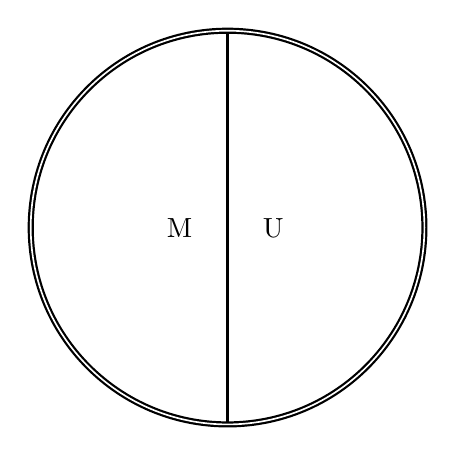
\begin{tikzpicture}[scale=.5]
			\draw[thick,double] (0,0) circle (5);
			\draw[thick] (0,-4.95) -- (0,4.95);
				\node[label={[label distance=2mm]180:M}] at (0,0) {};
				\node[label={[label distance=2mm]360:U}] at (0,0) {};
		\end{tikzpicture}}
\end{figure}
\chapter{Discourse driven metathesis} \label{ch:DisMet}

\SelectTips{lu}{12}
%\SelectTips{cm}{12}
%\SelectTips{eu}{12}

\section{Introduction}
In this chapter I analyse the morphological use of metathesis
in Amarasi to mark discourse structures.
The final member of a phrase or clause uses
metathesis to mark that the situation/event encoded
by the clause is unresolved and requires another clause to achieve resolution.
A discourse U-form (unmetathesised) typically
occurs in a parallel and complementary relationship
with an M-form (metathesised), the latter of which resolves the former.

Example \qf{ex:02/08/13, p.20 -2} is a question-answer
pair in which a question with a final U-form
is resolved by an answer in the M-form.
Example \qf{ex:130909-6, 0.39 -2} contains two events.
The second event is encoded in the M-form and is dependent
on the prior clause with a final U-form for its realisation.

\begin{exe}
	\ex{\glll \textnormal{\tcb{Q:}} hoo \bxA{mu-be\tbr{ʔi}}? \hspace{10mm} \textnormal{\tcb{A:}} au \bxB{u-be\tbr{iʔ}}! {\lk} \\
						{} hoo {\gp}mu-beʔi {} {} au {\gp}u-beʔi \\
						{} {\hoo} \gp\mu-capable{\tbrU} {} {} {\au} \gp\qu-capable{\tbrM} \\
						\lh{Q: }`Can you do it?' \hspace{19.75mm}`Yes I can!'
						\txrf{observation 02/08/13, p.20}}\vspace{4pt}\label{ex:02/08/13, p.20 -2} 
	\ex{\glll	m-ak hai nua =kai \bxA{m-taiko\tbr{bi}} =m hai \bxB{m-ma\tbr{et}} okeʔ {\lk}\\
						m-ak hai nua =kai {\gp}m-taikobi =ma hai {\gp}m-mate okeʔ \\
						\m-say {\hai} two {\kai} \gp\m-fall{\tbrU} =and {\hai} \gp\m-die{\tbrM} all \\
			\glt	`So we two will fall down and (then) both die.'
						\txrf{130909-6, 0.39} {\emb{130909-6-00-39.mp3}{\spk{}}{\apl}}}\label{ex:130909-6, 0.39 -2}
\end{exe}

Discourse U-forms are used by speakers to signal that
the event or situation is not resolved.
Such a U-form represents half of a whole
which requires resolution by another clause.
Discourse driven U-forms leave the audience in a state of  suspense
with the speaker signalling that more information
is required to resolve the situation or event
encoded by a clause with a final U-form.

Nearly all word classes which are not canonical nominals
(as defined in \srf{sec:NomWorCla}) have discourse driven U-forms.
These word classes are listed in \qf{ex:WorClaDisMet} below.
I refer to these word classes as ``non-nominals'' throughout this chapter.
The label `non-nominal' is not ideal as place names,
demonstratives and pronouns all have many nominal characteristics.
However, there does not seem to be a more appropriate term
which covers all of the word classes in \qf{ex:WorClaDisMet}.

\begin{exe}
	\ex{Word classes with discourse driven U-forms:}\label{ex:WorClaDisMet}
		\begin{xlist}
			\ex{verbs}
			\ex{numerals}
			\ex{place names}
			\ex{number enclitics (\ve{eni} `{\ein}', \ve{=esa}, {\es})}
			\ex{demonstratives (\ve{nana} {\naan})}
			\ex{determiners (\ve{=ana} {\aan})}
			\ex{pronouns (\ve{ini} {\iin}, \ve{sini} {\siin}, \ve{hiti} {\hiit})}
			\ex{adverbials (\ve{=ena} `{\een}', \ve{=aha} `just')}
		\end{xlist}
\end{exe}

The use of U-forms is productive for verbs, numerals, and place names.
For the other word classes listed in \qf{ex:WorClaDisMet},
particularly the number enclitic \ve{=eni} `{\ein}',
the adverbials \ve{=ena} `{\een}' or \ve{=aha} `just',
and the demonstratives and determiners,
the use of U-forms is less productive, though there
are still many instances in which U-forms with
these latter classes signal a lack of resolution.

Discourse U-forms typically occur in certain constructions and environments.
These constructions and environments include: dependent co-ordination (\srf{sec:DepCoo}),
tail-head linkage (\srf{sec:TaiHeaLin}), poetic parallelism (\srf{sec:PoePar}),
chiasmus (\srf{sec:CenChi}) and interactions between speakers (\srf{sec:IntUnm}).
These five constructions are summarised in \trf{tab:ConDisUfoTypOcc}
above along with the typical structure of each.
In my corpus there are 423 discourse driven U-forms.
Of these, 406 (96\%) clearly occur in one of the five
constructions/environments given in \trf{tab:ConDisUfoTypOcc}.\footnote{
		With 423 attestations, discourse (un)metathesis is a well attested morphological process.
		For comparison, my corpus has 152 instances of partial reduplication (\srf{sec:Red})
		and 48 of the reciprocal prefix \ve{ma(k)-} (\srf{sec:RecPre}).}

\begin{table}[ht]
	\caption[Constructions in which discourse U-forms typically occur]
					{Constructions in which discourse U-forms typically occur\su{†}}\label{tab:ConDisUfoTypOcc}
	\centering
		\begin{threeparttable}[b]
		\begin{tabular}{rll}
			\lsptoprule
			Construction & Typical Structure  &\\ \midrule
				&&\\[-6pt]
			Dependent Co-ordination &
				\xytext{\fbox{event\sub{1}{\U}}\xybarconnect[2][->]{2}&(conj.)&\fbox{event\sub{2}({\M})}} &\S\ref{sec:DepCoo}\\
				&&\\[-6pt]\hline
				&&\\[-3pt]
			Tail-head linkage & 
				\xytext{\fbox{event\sub{1}{\M}}\xybarconnect[2][-](D,D){1}&\fbox{event\sub{1}{\U}}\xybarconnect[2][->]{2}&(conj.)&\fbox{event\sub{2}\vp{\M}}} &\S\ref{sec:TaiHeaLin}\\
				&&\\[-6pt]\hline
				&&\\[-6pt]
			Poetic parallelism &
				\xytext{\fbox{synonym\sub{1}{\U}}\xybarconnect[2][-](D,D){2}\xybarconnect[2][->]{2}&conj.&\fbox{synonym\sub{2}{\M}}} &\S\ref{sec:PoePar}\\
				&&\\[-6pt]\hline
				&&\\[-3pt]
			Chiasmus & 
				\xytext{\fbox{information\sub{1}}\xybarconnect[2][-](D,D){2}\xybarconnect[2][<-]{1}&\fbox{U-form\vp{\sub{1}}}\xybarconnect[2][->]{1}&\fbox{information\sub{1}}} &\S\ref{sec:CenChi}\\
				&&\\[-6pt]\hline
				&&\\[-6pt]
			Interaction & 
				\xytext{Speaker\sub{1}:&\fbox{U-form}\xybarconnect[2][-](D,D){2}\xybarconnect[2][->]{2}&Speaker\sub{2}:&\fbox{M-form}} &\S\ref{sec:IntUnm}\\
				&&\\[-6pt] %\hline
				\lspbottomrule
				\end{tabular}
			\begin{tablenotes}
				\item [†] An arrow indicates the form which resolves a U-form
												and a line joining two forms indicates forms
												which are semantically identical or parallel.
												Event\sub{1} and event\sub{2} refer to
												two different events or situations,
												with event\sub{1} beginning before event\sub{2}.
			\end{tablenotes}
		\end{threeparttable}
\end{table}

Before I discuss the details of U-forms in Amarasi discourse,
I discuss several other facts which provide helpful background information:
the co-occurrence of syntactically driven M-forms
and discourse driven U-forms (\srf{sec:SynDisDriMet}),
the fact that the M-form is the semantically
unmarked form of non-nominals (\srf{sec:DefFor1}),
phonotactic constraints which block the use
of discourse U-forms (\srf{sec:PhoCon}),
and some of the general structures of Amarasi discourse (\srf{sec:DisStrAma}).

\section{Syntactically and discourse driven metathesis}\label{sec:SynDisDriMet}
Discourse driven U-forms occur with
the final members of phrases, while syntactically driven
M-forms occur with the medial members of phrases.
As a result, they are in complementary distribution and 
there is no competition between these two morphological uses of metathesis.
Two illustrative examples are given in \qf{ex2:160326, 5.37}
and \qf{ex2:160326, 18.26} below.

In \qf{ex2:160326, 5.37} the first member of the serial verb
construction \ve{ta-hiin t-ana} `figure out, get to know'
occurs in the M-form to mark that
it is modified by the second verb, as discussed in \srf{sec:SVC},
while the final verb occurs in the U-form
to signal that the entire verb phrase requires more information to achieve resolution.
See \qf{ex:160326, 5.37-5.45} on page \pageref{ex:160326, 5.37-5.45}
for more discussion of this example and its context.

\begin{exe}
	\ex{\glll	siin neem na-tua Koorʔoot ees reʔ oras mee \hspace{25mm} ka= ta-hi\tbr{in} t-a\tbr{na} =f.\\
						sini neem na-tua Koorʔoto esa reʔ oras mee {} ka= ta-hini t-ana =f.\\
						{\siin} {\nema} \na-settle Koro{\Q}oto{\M} {\esc} {\req} time where {} {\ka}= {\tg}-know{\tbrM} {\tg}-{\ana\tbrU} ={\fa}\\
			\glt	`They came and settled in Koro{\Q}oto, it was at a time which hasn't been figured out.'
						\txrf{160326, 5.37} {\emb{160326-05-37.mp3}{\spk{}}{\apl}}}\label{ex2:160326, 5.37}
\end{exe}

Similarly, in \qf{ex2:160326, 18.26} below the first member
of the noun phrase \ve{kaan auk-k=eni} `praise names' occurs in the M-form to signal
that it is modified by the following nominal,
as discussed in chapter \ref{ch:SynMet}.
This nominal in turn occurs in the M-form due to the following
vowel initial enclitic, as discussed in chapter \ref{ch:PhoMet}.
The final member of this phrase is the number enclitic \ve{=eni} `{\ein}'
which occurs in the U-form to signal that the entire phrase requires
more information to achieve resolution.
See \qf{ex:160326, 18.26} on page \pageref{ex:160326, 18.26}
for more discussion of this example.

\begin{exe}
	\ex{\glll	siin naiʔ Bain mone \sf{kusus}, \hspace{60mm} siin ka\tbr{an} a\tbr{uk}-k=e\tbr{ni} bisa, Mea aiʔ Tutun.\\
						sini naiʔ Bani mone \sf{kusus} {} sini kana aku-k=eni bisa Mea aiʔ Tutun\\
						{\siin} {\naiq} Bani{\M} male exclusive {} {\siin} name{\tbrM} praise.name{\tbrMv}-{\k=\ein\tbrU} can Mea or Tutun\\
			\glt	`Members of the Bani clan classified as male can
						exclusively have the praise names Mea or Tutun.'
						\txrf{160326, 18.26} {\emb{160326-18-26.mp3}{\spk{}}{\apl}}}\label{ex2:160326, 18.26}
\end{exe}

To summarise, syntactically driven M-forms only
occur with medial members of phrases, while discourse
driven U-forms only occur with final members of phrases.
As a result, there is no competition between them.
In a single phrase the medial members
can occur in the M-form to signal the internal
syntactic structure of the phrase, while the final
member can occur in the U-form to signal the discourse
status of the entire phrase.
\section{Default M-form}\label{sec:DefFor1}
For the non-nominal word classes given in \qf{ex:WorClaDisMet} above
the default semantic form is the M-form
(see \srf{sec:PhoCon} for exceptions).
Even though the M-form of these word classes is the semantically default form,
the U-form must still be posited as the morphologically underlying form.
This can be shown by the processes of vowel assimilation which occur
in the formation of M-forms (\srf{sec:VowAss}).
Two examples of minimal pairs with identical M-forms but different U-forms are
\ve{{\rt}nene} `press' and \ve{{\rt}nena} `hear' {\ra} \ve{n-neen} `presses'/`hears'
as well as \ve{{\rt}rene} `field' and \ve{{\rt}rena} `force' {\ra}
\ve{na-reen} `makes field'/`forces'.

For these word classes, the morphologically unmarked form
is the semantically marked form with special discourse uses (unresolved),
and the morphologically marked form is the semantically unmarked form without special discourse uses.
This difference between nominals and other word classes is shown in \trf{tab:NomVerMet}.

\begin{table}[h]
	\caption{Nominal and non-nominal metatheses}\label{tab:NomVerMet}
	\centering
		\begin{tabular}{rcc} \lsptoprule
							& unmarked	& marked\\
							& semantics	& semantics\\ \midrule
			nominal	& U-form		& M-form \\
			other		& M-form		& U-form \\ \lspbottomrule
		\end{tabular}
\end{table}

Most of discussion in this section focusses on verbs
as these are the most well attested word class with default M-forms,
though the statements also hold for the other non-nominal word classes.
The M-form of these word classes is the form used in simple declarative sentences,
the citation form and the most common form.
Three simple declarative sentences
are given in \qf{ex:130928-1, 0.02}--\qf{ex:120715-3, 0.10} below.
Each of these examples is taken from the very beginning of its text.
The verbs in each instance take the M-form.

\begin{exe}
	\ex{\glll	neno ia aam Nahor Bani iin n-ma\tbr{et}.\\
						neno ia ama Nahor Bani ini n-mate\\
						day {\ia} father Nahor Bani {\iin} {\n}-die{\tbrM}\\
			\glt	`Today father Nahor Bani died.'
						\txrf{130928-1, 0.02} {\emb{130928-1-00-02.mp3}{\spk{}}{\apl}}}\label{ex:130928-1, 0.02}
	\ex{\glll	krei ia iin naan-n=ii, hai m-re\tbr{es} surat Roma.\\
						krei ia ini nana-n=ii, hai m-resa surat Roma\\
						week {\ia} {\iin} inside-{\N}={\ii} {\hai} {\m}-read{\tbrM} paper Romans\\
			\glt	`During this week we read the book of Romans.'
						\txrf{130920-1, 0.22} {\emb{130920-1-00-22.mp3}{\spk{}}{\apl}}}\label{ex:130920-1, 0.22}
	\ex{\glll	ahh, hai m-baise\tbr{un} fuunn=ee =te, ahh\\
						{} hai m-baisenu funan=ee =te {}\\
						{} {\hai} {\m}-look.up{\tbrM} moon={\ee} ={\te} {}\\
			Umm, when we looked up at the moon,'
						\txrf{120715-3, 0.10} {\emb{120715-3-00-10.mp3}{\spk{}}{\apl}}}\label{ex:120715-3, 0.10}
\end{exe}

As the default form, the M-form is also the usual citation form.
The citation forms of a number of vowel final verbs and numerals in one recorded
word-list are given in \qf{ex:VowFinVerCitFor} below.
Verbs occur with the \tsc{3sg} agreement market \ve{(a|)n-} or \ve{na-}.

\begin{exe}
	\ex{Vowel final verb and numeral citation forms:}\label{ex:VowFinVerCitFor}
	\sn{\gw\begin{tabular}{llll}
				Root					&		&Citation							& \\
				\ve{\rt henu}	&\ra&\ve{na-he\tbr{un}}		&`fill, is full'\\
				\ve{\rt hini}	&\ra&\ve{na-hii\tbr{in}}	&`know'\\
				\ve{\rt ita}	&\ra&\ve{n-i\tbr{it}}			&`look at'\\
				\ve{\rt kisu}	&\ra&\ve{a|n-ki\tbr{us}}	&`see'\\
				\ve{\rt mate}	&\ra&\ve{n-ma\tbr{et}}		&`die'\\
				\ve{\rt nena}	&\ra&\ve{a|n-ne\tbr{en}}	&`hear'\\
				\ve{\rt roʔa}	&\ra&\ve{a|n-ro\tbr{oʔ}}	&`vomit'\\		
				\ve{\rt roro}	&\ra&\ve{a|n-ro\tbr{or}}	&`kill by stabbing'\\
				\ve{\rt tenu}	&\ra&\ve{te\tbr{un}}	&`three'\\
				\ve{\rt nima}	&\ra&\ve{ni\tbr{im}}	&`five'\\
				\ve{\rt hitu}	&\ra&\ve{hi\tbr{ut}}	&`seven'\\
				\ve{\rt fanu}	&\ra&\ve{fa\tbr{un}}	&`eight'\\
		\end{tabular}}
\end{exe}

For nominals, the semantically default form is the U-form,
with the M-form marking modification (see chapter \ref{ch:SynMet}).
There are a number of roots in Amarasi
which can occur as either a verb or nominal,
such roots are cited in U-form for the nominal meaning
and the M-form for the verbal meaning.
Examples are given in \trf{tab:AmaNomVerPai} below.

\begin{table}[h]
	\caption{Citation forms of noun-verb pairs}\label{tab:AmaNomVerPai}
	\centering
		\begin{tabular}{lllll} \lsptoprule
			Root						&Nom.								&Gloss (N.)		&Verb									& Gloss (V.) \\ \midrule
			\ve{\rt heʔo}		&\ve{he\tbr{ʔo}}		&`(a) saw'		&\ve{n-he\tbr{oʔ}}		&`(to) saw' \\
%			\ve{\rt kinu}		&\ve{ki\tbr{nu}-f}	&`cheek'			&\ve{na-ki\tbr{un}}		&`(to) spit' \\
			\ve{\rt ʔsoko}	&\ve{ʔso\tbr{ko}}		&`sign'				&\ve{na-ʔso\tbr{ok}}	&`make a sign' \\
			\ve{\rt nope}		&\ve{no\tbr{pe}}		&`cloud'			&\ve{n-no\tbr{ep}}		&`be cloudy' \\
			\ve{\rt reko}		&\ve{re\tbr{ko}}		&`good'				&\ve{na-re\tbr{ok}}		&`be good' \\
			\ve{\rt rono}		&\ve{ro\tbr{no}-f}	&`saliva'			&\ve{n-ro\tbr{on}}		&`(to) spit' \\
			\ve{\rt siʔu}		&\ve{si\tbr{ʔu}-f}	&`(an) elbow'	&\ve{n-si\tbr{uʔ}}		&`(to) elbow' \\
			\ve{\rt snasa}	&\ve{sna\tbr{sa}-f}	&`breath'			&\ve{na-sna\tbr{as}}	&`take a break' \\
%			\ve{\rt tika}		&\ve{ti\tbr{ka}-f}	&`heel'				&\ve{na-ti\tbr{ik}}		&`(to) stamp' \\
		%	\ve{\rt }	&\ve{}	&\ve{}	&`'	&`' \\
		\lspbottomrule
		\end{tabular}
\end{table}

The M-form is also the most frequent form for non-nominals.
In my corpus M-forms comprise 73{\%} (3,858/5,271) of non-nominals.
After excluding M-forms which are obligatory before vowel initial enclitics
(544 instances), U-forms which are consonant final stems (556 instances),
and U-forms before consonant clusters (435 instances),
M-forms constitute 89{\%} (3,313/3,736) of the relevant word classes.
Put differently, the semantically unmarked form occurs in 89{\%} of instances.
The figures for each word class are detailed in \trf{tab:FreUfoMfoTex}.

\begin{table}[h]
	\caption[Frequency of U-forms and M-forms in texts]
					{Frequency of U-forms and M-forms in texts\su{†}}\label{tab:FreUfoMfoTex}
	\centering
		\begin{threeparttable}[b]
			\begin{tabular}{rllll|lll}\lsptoprule
					&	U-form	&	/{\gap}CC	&	/C{\#}	&	else.	&	M-form	&	/{\gap}=V	&	else.	\\	\midrule
				verbs	&	1,077	&	350	&	441	&	286	&	1,913	&	440	&	1,473	\\	
				numerals	&	41	&	2	&	26	&	13	&	76	&	25	&	51	\\	
				place names	&	99	&	0	&	89	&	10	&	51	&	4	&	47	\\	
				\ve{esa/=esa}	&	79	&	41	&	0	&	38	&	375	&	39	&	336	\\	
				eni	&	21	&	3	&	{--}	&	18	&	171	&	26	&	145	\\	
				pronouns	&	46	&	30	&	{--}	&	16	&	987	&	10	&	977	\\	
				dem./det.	&	24	&	4	&	{--}	&	20	&	144	&	0	&	144	\\	
				\ve{=ena/=aha}	&	27	&	5	&	{--}	&	22	&	140	&	0	&	140	\\	
				total	&	1,414	&	435	&	556	&	423	&	3,857	&	544	&	3,313	\\	
			\lspbottomrule
			\end{tabular}
			\begin{tablenotes}
				\item [†] U-form = total U-forms,
									/{\gap}CC = U-forms before consonant clusters,
									/C{\#} = consonant final stems in U-form,
									else. = U-forms elsewhere (discourse driven U-forms),
									M-form = total M-forms,
									/{\gap}=V = M-forms before vowel initial enclitics,
									else. = other M-forms
			\end{tablenotes}
		\end{threeparttable}
\end{table}

M-forms are the semantically default form for verbs,
numerals, number enclitics, place names, pronouns, demonstratives,
determiners and adverbials.
For these word classes U-forms normally mark
an unresolved event or situation.

\section{Phonotactic constraints}\label{sec:PhoCon}
There are several phonotactic/phonological environments
which block the use of U\=/forms to signal lack of resolution.
The end result of these different phonotactic constraints
is that only non-nominals which end in CV{\#}
have morphological uses of U\=/forms, and then only
when not followed by a vowel-initial enclitic or
word with an initial consonant cluster.

Firstly, and most obviously, stems which end a vowel
sequence do not have (surface) alternate
U\=/forms and M\=/forms (\srf{sec:NoCha}).
Thus, such stems cannot use U\=/forms to
morphologically signal lack of resolution.

Other situations in which the phonology overrides or blocks
the morphology with the result that U\=/forms do not mark lack of resolution
include when vowel-initial enclitics occur attached to a stem (\srf{sec:PhoCon sec:VowIniEnc}),
when a stem is consonant final (\srf{sec:ConFinVer}),
and when a stem is followed by a consonant cluster (\srf{sec:VerBefCC}).
Each of these different environments is discussed in turn in the following sections.

\subsection{Vowel-initial enclitics}\label{sec:PhoCon sec:VowIniEnc}
As discussed in Chapter \ref{ch:PhoMet},
M\=/forms are obligatory before vowel-initial enclitics.
When a non-nominal occurs with a vowel-initial enclitic,
it obligatorily occurs in the M\=/form and it is
not possible to mark lack of resolution with the clitic host.
However, if the vowel-initial enclitic itself has alternate
U\=/forms and M\=/forms, lack of resolution of the clause can
be signalled by this vowel-initial enclitic taking the U\=/form.
One example is given in \qf{ex:HooMfaanJena} below
-- a typical question asked around the village.

\begin{exe}
	\ex{\glll	hoo {m-faan\j=e\tbr{na} ?}\\
						hoo m-fani=ena \\
						{\hoo} \m-return{\Mv=\een\tbrU}\\
			\glt	`So, you're going back now?'
						\txrf{observation}}\label{ex:HooMfaanJena}
\end{exe}

In \qf{ex:HooMfaanJena} the clitic host \ve{m-faan\j} `return'
occurs in the M\=/form due to the following vowel-initial enclitic.
As a result, it is not possible to mark
that this is a question with this stem
(see \srf{sec:IntUnm} for full discussion of
the use of U\=/forms to mark questions).
Instead, the vowel-initial enclitic occurs in the U\=/form
to signal that this clause is a question.

If the vowel-initial enclitic itself does not have metathesis
alternations, i.e. if the vowel-initial enclitic ends in a vowel sequence,
it is not possible to morphologically mark lack of resolution.

\subsection{Consonant-final U\=/forms}\label{sec:ConFinVer}
Non-nominal stems with a final consonant occur by default in the U\=/form
and do not use U\=/forms to morphologically signal lack of resolution.
Consonant-final non-nominals only occur in the M\=/form
before vowel-initial enclitics.
Consonant-final U\=/forms are glossed {\Uc}
-- U with a \emph{c} for consonant above it --
to mark that these are not discourse-driven U\=/forms.
Two examples of simple declarative sentences with
consonant-final verbs occurring in the U\=/form
are given in \qf{ex2:120715-4, 0.05} and \qf{ex:130823-2, 0.57} below.

\begin{exe}
	\ex{\gll	neno naa paha{\gap}ʔpina-n ia, \hp{3-pile.up{\Uc} {\on} place} a|n-ko\tbr{bub} on bare meseʔ\\
						day {\naa} country{\gap}below-{\N} {\ia} {} {\a\n}-pile.up{\tbrUc} {\on} place one\\
			\glt	`In those days the world was piled up in one place.'
						\txrf{120715-4, 0.05} {\emb{120715-4-00-05.mp3}{\spk{}}{\apl}}}\label{ex2:120715-4, 0.05}
	\ex{\gll	n-ak: ``hiit ta-na\tbr{niʔ} kuan=ii, kaisaʔ Neanpeen. \\
						{\n}-say	\hphantom{``}{\hiit} {\ta}-move{\tbrUc} village={\ii} {\kais} Neanpeen\\
			\glt `They said: ``Let's change the village, it shouldn't be Neanpeen.'
						\txrf{130823-2, 0.57} {\emb{130823-2-00-57.mp3}{\spk{}}{\apl}}}\label{ex:130823-2, 0.57}
\end{exe}

Similarly, the citation form of consonant-final verbs is the U\=/form.
Examples of consonant-final verbs cited in the U\=/form in a recorded wordlist
are given in Table \qf{ex:ConFinVerCitFor} below.

\begin{exe}
	\ex{Consonant-final verb citation forms:}\label{ex:ConFinVerCitFor}
	\sn{\gw\begin{tabular}{llll}
			 Root							&		&Citation								& \\
			 \ve{\rt ʔapuʔ}	&\ra&\ve{na-ʔa\tbr{puʔ}} 	& `is pregnant'\\
			 \ve{\rt manis} 	&\ra&\ve{n-ma\tbr{nis}} 		& `laughs at s.o.'\\
			 \ve{\rt reruʔ}	&\ra&\ve{a|n-re\tbr{ruʔ}}	& `is sleepy'\\
			 \ve{\rt sumak}		&\ra&\ve{a|n-su\tbr{mak}} 	& `dives'\\
		\end{tabular}}
\end{exe}

This behaviour includes verbs whose final consonant is a suffix,
or the consonantal allomorph of the plural enclitic \ve{=n}.
%Suffixes which consist of a single consonant in Amarasis
%include the transitive suffixes \ve{-b} and \ve{-ʔ} (\srf{sec:TraSuf}).
The citation forms of a number of vowel-final verbs
and their corresponding forms with the plural enclitic \ve{=n}
are given in \qf{ex:PluVer} below to illustrate.

\begin{exe}
	\ex{Plural verb citation forms:}\label{ex:PluVer}
	\sn{\gw\begin{tabular}{lllll}
			 Root					& Verb	&			& Verb={\einV} 			& \\
			\ve{\rt nema}	&	\ve{neem}		&\ra&\ve{ne\tbr{ma}=\tbr{n}}	&`come' \\
			\ve{\rt tona}	&	\ve{na-toon}&\ra&\ve{na-to\tbr{na}=\tbr{n}}	&`tell' \\
			\ve{\rt mate}	&	\ve{n-maet}	&\ra&\ve{n-ma\tbr{te}=\tbr{n}}	&`die' \\
			\ve{\rt eki}	&	\ve{n-eik}	&\ra&\ve{n-e\tbr{ki}=\tbr{n}}		&`bring' \\
			\ve{\rt hini}	&	\ve{na-hiin}&\ra&\ve{na-hi\tbr{ni}=\tbr{n}}	&`know' \\
			\ve{\rt mepu}	&	\ve{n-meup}	&\ra&\ve{n-me\tbr{pu}=\tbr{n}}	&`work' \\
			\ve{\rt romi}	&	\ve{n-roim}	&\ra&\ve{n-ro\tbr{mi}=\tbr{n}}	&`like' \\
		\end{tabular}}
\end{exe}

Ro{\Q}is Amarasi behaves differently in this respect
as stems in which the penultimate or final consonant
is /n/ occur in the M\=/form (and with a final consonant cluster) by default.
U\=/forms of such stems are then used to signal lack of resolution.
Two examples of Ro{\Q}is Amarasi sentences with a consonant-final
verb in the M\=/form are given in \qf{ex:08/10/14, p.113}
and \qf{ex:09/10/14, p.114} below.
See \srf{sec:DisDriMetRoqAma} for more discussion of the
use of M\=/forms with a final cluster in Ro{\Q}is Amarasi.

\begin{exe}\let\eachwordtwo=\itshape
	\ex{\glll	\textnormal{\tcb{Ro{\Q}is:}} siin na-sa\tbr{ap}=\tbr{n}.\\
						\textnormal{\tcb{Kotos:}} siin na-sa\tbr{pa}=\tbr{n}.\\
						{} {\siin} {\na}-kick={\einV}\\
			\glt	\lh{Kotos: }`They're playing soccer.'
						\txrf{observation 08/10/14, p.113}}\label{ex:08/10/14, p.113}
	\ex{\glll	\textnormal{\tcb{Ro{\Q}is:}} raump=ein n-ma\tbr{et}=\tbr{n}.\\
						\textnormal{\tcb{Kotos:}} paku=n n-ma\tbr{te}=\tbr{n}.\\
						{} light={\ein} {\n}-die={\einV}\\
			\glt	\lh{Kotos: }`The lights have died.'
						\txrf{observation 09/10/14, p.114}}\label{ex:09/10/14, p.114}
\end{exe}

Consonant-final non-nominals in Kotos
Amarasi take the U\=/form by default.
Such words do not have metathesis alternations
to express discourse functions.

\subsection{U\=/forms before consonant clusters}\label{sec:VerBefCC}
Another phonotactic environment in which non-nominals
do not usually occur in the M\=/form is before consonant clusters.\footnote{
		Functors often occur in the M\=/form before consonant clusters.
		This is connected with the fact that the use of the U\=/form
		with functors is not fully productive.}
Before a consonant cluster the usual form of a non-nominal is
the U\=/form and lack of resolution is not morphologically marked.
This is similar to the fact that certain nouns do
not undergo metathesis before modifiers with an initial consonant cluster,
and thus cannot morphologically mark attributive modification (\srf{sec:CVFinWor}).

Like U\=/forms with a word-final consonant, U\=/forms before a consonant cluster
are glossed {\Uc} to distinguish them from discourse-driven U\=/forms.
In my corpus there are over 300 U\=/forms of verbs before a consonant
cluster and only 21 verbal M\=/forms before a consonant cluster.
Two examples of a U\=/form before a consonant cluster initial root are given in
\qf{130825-6, 10.05} and \qf{ex:130914-1, 0.53} below.

\begin{exe}
	\ex{\glll	uma ʔ-tee =ma, ʔ-ai\tbr{ti} \tbr{br}uuk.	\\
						uma ʔ-tea =ma ʔ-aiti bruuk \\
						{\uma\Uc} \q-arrive =and \q-pick.up{\tbrUc} pants	\\
			\glt	`I arrived (home) and picked up some pants.' \txrf{130825-6, 10.05} {\emb{130825-6-10-05.mp3}{\spk{}}{\apl}}}\label{130825-6, 10.05}
	\ex{\gll	{onai =te}, hoo m-te\tbr{bi} \tbr{ʔt}etaʔ.\\
						like.this  {\hoo} {\m}-turn{\tbrUc} different\\
			\glt	`Like this, you turn (it) differently.'
						\txrf{130914-1, 0.53} {\emb{130914-1-00-53.mp3}{\spk{}}{\apl}}}\label{ex:130914-1, 0.53}
\end{exe}

One of the most frequent kinds of consonant clusters in my corpus
are those created through the addition of a verbal prefix 
to a consonant-initial verb stem (\srf{sec:Pre}).
This is the most common kind of consonant cluster found after verbal U\=/forms.
Two examples are given in \qf{ex:130902-1, 3.41} and \qf{ex:120715-4, 2.26} below.

\begin{exe}
	\ex{\gll	hai m-e\tbr{ki} \tbr{m}-\tbr{s}a\tbr{nu} \tbr{m}-\tbr{b}i reʔ ʔpinan ia =t,\\
						{\hai} {\m}-bring{\tbrUc} {\m}-go.down{\tbrUc} {\m}-{\bi} {\reqt} below {\ia} ={\te}\\
			\glt	`When we went down there,'
						\txrf{130902-1, 3.41} {\emb{130902-1-03-41.mp3}{\spk{}}{\apl}}}\label{ex:130902-1, 3.41}
	\ex{\glll	iin ao-n=ee n-me\tbr{se} \tbr{n}-\tbr{n}ao n-peoʔ aafgw=ii =m,\\
						ini ao-n=ee n-mese n-nao n-peʔo afu=ii =ma\\
						{\iin} body-{\N}={\ee} {\n}-alone{\tbrUc} {\n}-go {\n}-go.by{\M} ground={\ii} =and\\
			\glt	`His body went by itself along the ground.'
						\txrf{120715-4, 2.26} {\emb{120715-4-02-26.mp3}{\spk{}}{\apl}}}\label{ex:120715-4, 2.26}
\end{exe}

While the vast majority of non-nominals are in the U\=/form before a consonant cluster,
there are 15 instances of an M\=/form before such words in my corpus.
Such examples represent only 7{\%} (21/302) of all verbs before a consonant cluster.
Two examples are given in \qf{ex:130907-3, 8.04} and \qf{ex:160326, 10.22} below.

\begin{exe}
	\ex{\glll	surat a|n-poi n-taa\tbr{m} \tbr{n}-\tbr{p}oi n-taam, au ʔ-toup.\\
						surat {\a}n-poi n-tama n-poi n-tama au ʔ-toup\\
						paper{\U} {\a\n}-exit {\n}-enter{\tbrM} {\n}-exit {\n}-enter{\M} {\au} {\q}-receive{\M}\\
			\glt	`Letters would be issued and received, issued and received, I got (one).'
						\txrf{130907-3, 8.04} {\emb{130907-3-08-04.mp3}{\spk{}}{\apl}}}\label{ex:130907-3, 8.04}
	\ex{\glll	n-ei\tbr{k} \tbr{kr}ee\j=ii neem. \\
						n-eki krei=ii nema	\\
						\n-bring{\tbrM} church={\ii} {\nema\M}\\
			\glt `(They) brought the Church here.'
						\txrf{160326, 10.22} {\emb{160326-10-22.mp3}{\spk{}}{\apl}}}\label{ex:160326, 10.22}
%	\ex{\glll	ʔ-istarii\tbr{k} \tbr{br}uuk pasan nima\\
%						ʔ-istarika bruuk pasan nima\\
%						\q-iron{\U} pants set{\U} five{\U}\\
%			\glt	`I ironed five sets of pants.' \txrf{130825-6, 10.50}}\label{ex:130825-6, 10.50}
\end{exe}

%nta'-taa' nbi
%surat anpoi ntaam npoi ntaam, 'toup.
%ntoom nsaen nafani'
%Iim arkit atneen hiit t'aa' tsaeb a'piru' baru
%'istariik bruuk pasan nima.
%'meup 'aan toon bo' haa nbi krei jit, usnaas 'po-'poi neno ia.
%atfoi' 'sui'n ee msa' ate ka bisa fa

\subsubsection{Consonant-final stems before consonant clusters}\label{sec:ConFinaVerBefCC}
There are 44 instances of a consonant-final
stem before a consonant cluster in my corpus.
In 14 instances, epenthesis (\srf{sec:Epe})
occurs to break up the underlying cluster of three consonants.
Two examples are given in \qf{ex:130913-1, 2.30} and \qf{ex:120715-4, 1.52} below.

\begin{exe}
	\ex{\glll	t-pe{\tl}pea mes \sf{baap} \sf{tua} Banus iin na-bara\tbr{b} \tbr{a}|\tbr{n}-\tbr{r}air\\
						t-pe{\tl}peo mes \sf{bapa} \sf{tua} Banus ini na-barab {\a}n-rari\\
						{\t}-{\prd}talk but father old Banus {\iin} {\na}-prepare{\tbrUc} {\a\n}-finish{\M}\\
			\glt	`We talk about it, but father Banus is already prepared.'
						\txrf{130913-1, 2.30} {\emb{130913-1-02-30.mp3}{\spk{}}{\apl}}}\label{ex:130913-1, 2.30}
	\ex{\glll	iin n-mooʔ\j=oo-n on kaunʔ=ii =ma n-nono\tbr{k} \tbr{a}|\tbr{n}-peoʔ aafgw=ii =ma\\
						ini n-moʔe=oo-n on kaunaʔ=ii =ma n-nonok {\a}n-peʔo afu=ii =ma\\
						{\iin} n-do{\Mv}={\oo-\N} {\on} snake={\ii} =and \n-crawl{\tbrUc} \a\n-go.by ground={\ii} =and\\
			\glt	`he did it like the snake and crawled along the ground'
						\xrf{120715-4, 1.52} {\emb{120715-4-01-52.mp3}{\spk{}}{\apl}}}\label{ex:120715-4, 1.52}
\end{exe}

In the remaining 30 examples in my corpus
the cluster of three consonants is not phonemically resolved.
In all but one case, the first consonant (i.e. the final consonant of the stem)
is either the glottal stop /ʔ/ or the alveolar nasal /n/.
That epenthesis is not obligatory after these consonants
is consistent with the data presented in \srf{sec:Epe},
which showed that epenthesis is uncommon between ʔ{\gap}CC,
and only optional between n{\gap}CC.

An example each of final /ʔ/ and /n/ before a consonant cluster
is given in \qf{ex:120923-2, 6.28} and \qf{ex:120715-4, 7.56} below respectively.
In both instances the first consonant of each cluster
is phonetically deleted, or has coalesced with the following consonant.

\begin{exe}\let\eachwordone=\textnormal \let\eachwordtwo=\itshape
	\ex{\glll	[i napɐpɐ \hp{=}mə̆ nsiɾ̞i \tbr{nˑ}aɔ̯̆ ˈpiʉ̞t]\\
						\hp{[}iin na-papaʔ =ma n-siri\tbr{ʔ} \tbr{n}-\tbr{n}ao piut.\\
						\hp{[}{\iin} {\na}-wound{\Uc} =and {\n}-spread{\tbrUc} {\n}-go continue\\
			\glt	\lh{[}`The wound keeps on spreading.'
						\txrf{120923-2, 6.28} {\emb{120923-2-06-28.mp3}{\spk{}}{\apl}}}\label{ex:120923-2, 6.28}
	\ex{\glll	[n͡maˈsenʊn \hp{=}{ɐmːɐ} ʔanmɐˈβanə \tbr{nβ}in \hspace{20mm} \hp{[}ɾɛ̰ʔ nanɐ̰ mɛsɛʔ]\\
						\hp{[}n-ma-senu=n =ama \hp{ʔ}a|n-ma-bana=\tbr{n} \tbr{n}-bi=n {} \hp{[}reʔ nanaʔ meseʔ\\
						\hp{[}{\n}-{\mak}-replace{\Uc}={\einV} =and \hp{ʔ}{\a\n\mak}-hit{\tbrUc}={\einV} {\n}-{\bi}={\einV} {} \hp{[}{\req} inside but\\
			\glt	\lh{[}`They replaced and fought one another inside.'
						\txrf{120715-4, 7.56} {\emb{120715-4-07-56.mp3}{\spk{}}{\apl}}}\label{ex:120715-4, 7.56}
\end{exe}

Verbs nearly always take the U\=/form
before a word which begins with a consonant cluster.
This is because clusters of three consonants are
normally disallowed in Kotos Amarasi.

\subsection{Summary}
There are a number of word classes in Amarasi for which the default form is the M\=/form
and for which the U\=/form is used to signal lack of resolution.
These word classes were listed in \qf{ex:WorClaDisMet} above,
repeated as \qf{ex:WorClaDisMet2} below.

\begin{exe}
	\ex{Word classes with discourse-driven U\=/forms:}\label{ex:WorClaDisMet2}
		\begin{xlist}
			\ex{verbs}
			\ex{numerals}
			\ex{place names}
			\ex{number enclitics (\ve{eni} `{\ein}', \ve{=esa}, `{\es}')}
			\ex{demonstratives (\ve{nana} `{\naan}')}
			\ex{determiners (\ve{=ana} `{\aan}')}
			\ex{pronouns (\ve{ini} `{\iin}', \ve{sini} `{\siin}', \ve{hiti} `{\hiit}')}
			\ex{adverbials (\ve{=ena} `{\een}', \ve{=aha} `just')}
		\end{xlist}
\end{exe}

Given the phonotactic constraints discussed in this section,
it is more accurate to say
that members of these word classes which end in CV{\#}
have discourse-driven U\=/forms when they do not occur
before a vowel-initial enclitic or a word with an initial consonant cluster.

U\=/forms of consonant-final non-nominals and U\=/forms of non-nominals
before a consonant cluster are glossed {\Uc} when it is necessary
to gloss them to distinguish them from U\=/forms which
are used morphologically to mark lack of resolution.

\section{Discourse structures in Amarasi}\label{sec:DisStrAma}
In this section I discuss the general patterns of Amarasi discourse
by means of a detailed exposition of a single short text.
This section provides the background for properly
understanding the discourse functions of U\=/forms.

The text selected for exposition is \it{Kuareno{\Q}},
a short narrative text about how the village of \it{Kuareno{\Q}}
came to have its current name.\footnote{
	The name \it{Kuareno{\Q}} is historically from
	\ve{kuan} `village' + \ve{ʔrenoʔ} `orange \it{Citrus sinensis}'.}
With sixteen clauses, this text is both short enough to allow detailed exposition,
and still long enough to illustrate a range of discourse structures.
The structure of this text is indicative of other texts.

The outline of this story is given in \trf{tab:SumKuaSto}.
In this table I have given a summary of each clause,
the part of the plot in which it occurs, which conjunctions occur
and the occurrence of U\=/forms and M\=/forms on non-nominals.\footnote{
		Recall that `{\Ucc}' is a consonant-final U\=/form,
		or U\=/form before a consonant cluster.
		As discussed in \srf{sec:DefFor1},
		the default form in such phonotactic environments is the U\=/form.
		`{\Mvv}' is an M\=/form before a vowel-initial enclitic.
		As discussed in Chapter \ref{ch:PhoMet}, M\=/forms
		are obligatory before vowel-initial enclitics.}
I have also tracked repetition between clauses with the use of capital letters,
each of which tracks a unique concept which is repeated.
Thus, the \emph{A} in clauses 1, 2, 13, 14, and 16 indicates
that each of these clauses contains the same concept
(which is not repeated elsewhere), in this case \ve{Kuarenoʔ} `Kuareno{\Q}'.
Similarly, \emph{D} in clauses 5 and 6 indicates that these clauses
contain the same concept, in this case \ve{ʔrenoʔ} `orange tree'.

\begin{table}[h]
	\caption{Summary of Kuareno{\Q} story}\label{tab:SumKuaSto}
	\centering\stl{0.25em}
		\begin{tabular}{rl@{\hspace{0.01em}}rllccccl} \lsptoprule
				&Plot&\mc{1}{l}{Conj.}&Summary		&\tsc{u/m}			&\mc{4}{l}{Repetition}&Index\\ \midrule
				1&\it{Opening}	&& Kuareno{\Q}'s name is K. because	&\tsc{{\Ucc}} \tsc{{\Ucc}}&A&B& & &\qf{ex:130823-2, 0.00}\\ \hline
				2&\it{Setting}	&& at first, its name wasn't K.			&\tsc{u} \tsc{{\Ucc}}			&A&B& & &\qf{ex:130823-2, 0.09}\\
				3&				&& its name was Neanpeen 									&\tsc{m}									& &B&C& &\qf{ex:130823-2, 0.13}\\
				4&				&& there were lots of people							&\tsc{m}									& & & & &\qf{ex:130823-2, 0.17}\\ \hline
				5&\it{Inciting}	&then& they planted an orange tree	&\tsc{m} \tsc{{\Ucc}}			&D& & & &\qf{ex:130823-2, 0.22}\\
				6&\it{incident}	&& a single orange tree 						&													&D& & & &\qf{ex:130823-2, 0.29}\\ \hline
				7&\it{Climax}		&then& it grew two branches 				&													&E& & & &\qf{ex:130823-2, 0.31}\\
				8&				&& it grew two branches 									&													&E& & & &\qf{ex:130823-2, 0.34}\\
				9&				&& one of the branches										&													&F& & & &\qf{ex:130823-2, 0.36}\\
				10&				&& its contents and fruit were red				&													&G&G& & &\qf{ex:130823-2, 0.42}\\
				11&				&& one was white													&													&G& & & &\qf{ex:130823-2, 0.45}\\
				12&				&& one of the branches was white					&													&F& & & &\qf{ex:130823-2, 0.49}\\ \hline
				13&\it{Dénouement}&so& someone called it K.					&\tsc{{\Mvv}} \tsc{{\Ucc}}&A&B& & &\qf{ex:130823-2, 0.51}\\
				14&\mc{2}{r}{so}& they named it K.									&\tsc{{\Mvv}}							&A&B& & &\qf{ex:130823-2, 0.55}\\
				15&				&& let's change it, not Neanpeen					&\tsc{{\Ucc}} \tsc{m}			& & &C&H&\qf{ex:130823-2, 0.56}\\
				16&				&but& let's change its name to K.					&\tsc{{\Mvv}} \tsc{{\Ucc}}&A&B& &H&\qf{ex:130823-2, 0.59}\\ %\hline
%				17&\it{Closure}&& that's it													&								& & & & &\qf{ex:130823-2, 1.03}\\
				\lspbottomrule
		\end{tabular}
\end{table}

I have broken the text up according to the plot structure,
and discuss each chunk in turn.
The identification of different parts of the
plot follows the principles and protocols outlined in \citet{dole01}.
Parts of each chunk which receive special discussion
are indicated in boldface type.

Line \qf{ex:130823-2, 0.00} is the Opening of the story.
After gathering his thoughts,
the narrator provides a short explanation that the text
is about the name of \it{Kuareno{\Q}} village.

\begin{exe}
	\ex{Kuareno{\Q} -- opening: \txrf{130823-2} {\emb{130823-2-00-00.mp3}{\spk{}}{\apl}}}\label{ex:130823-2, 0.00}
		\sn{\glll	ahh, {Kuarenoʔ ahh}, iin kaan-n=ee Kuarenoʔ {na-tuinaʔ ahh}\\
							{} Kuarenoʔ ini kana-n=ee Kuarenoʔ na-tuinaʔ \\
							{}  Kuareno{\Q}{\Uc} {\iin} name-{\N=\ee} Kuareno{\Q}{\Uc} {\na}-because \\
				\glt	`Umm, Kuareno{\Q}, its name is Kuareno{\Q} because,' \txrf{0.00}}
\end{exe}

This opening line is followed by the setting,
given as \qf{ex:130823-2, 0.09-0.17} below.
The Setting is the part of the story in which the narrator provides
background information about the place, time, and participants of the story.
In \qf{ex:130823-2, 0.09-0.17} we learn the time this story
took place (`long ago, at first') and more about the main participant, the village of Kuareno{\Q}.

\begin{exe}
	\ex{Kuareno{\Q} -- Setting: \txrf{130823-2} {\emb{130823-2-00-09-00-17.mp3}{\spk{}}{\apl}}}\label{ex:130823-2, 0.09-0.17}
	\begin{xlist}
		\ex{\glll	na-hu\tbr{nu} =\tbr{t}, iin kaan-n=ee ka= Kuarenoʔ =fa.\\
							na-hunu =te ini kana-n=ee ka= Kuarenoʔ =fa\\
							{\na}-first{\tbrU} {=\tbr{\te}} {\iin} name-{\N=\ee} {\ka}= Kuareno{\Q}{\Uc} ={\fa}\\
				\glt	`Well, at first its name wasn't Kuareno{\Q}.' \txrf{0.09}}\label{ex:130823-2, 0.09}
		\ex{\glll	iin kaan-n=ee ahh Neanpeen.\\
							ini kana-n=ee {} Neanpeen\\
							{\iin} name-{\N=\ee} {} Neanpeen{\M}\\
				\glt	`Its name was Neanpeen.' \txrf{0.13}}\label{ex:130823-2, 0.13}
		\ex{\glll	a|n-nao{\tl}nao =\tbr{te}, a|n-muiʔ toogw=ii na-mfau.\\
							{\a}n-nao{\tl}nao =te, {\a}n-muʔi too=ii na-mfau\\
							\a\n-{\frd}go {=\tbr{\te}} {\a\n}-have{\M} citizen={\ii} {\na}-many\\
				\glt	\lh{\a}`After a while, it had a lot of residents.' \txrf{0.17}}\label{ex:130823-2, 0.17}
	\end{xlist}
\end{exe}

In \qf{ex:130823-2, 0.09} there is a purely discourse
driven U\=/form; \ve{na-hunu} `at first; long ago',
which is resolved by the following two clauses
which describe the situation which held `long ago'.

In \qf{ex:130823-2, 0.09-0.17} there are also two occurrences of
the connector \ve{=te}, glossed as ={\te} `subordinator'.
This particle marks that the preceding clause is temporally
subordinate to the following clause.
This particle is always clause final and provides the background
which sets the scene for the following clause.
The clause preceded by \ve{=te} is the stage
on which the following clause takes place.

In \qf{ex:130823-2, 0.09} the clause \ve{na-hunu} `at first'
is the time of the next clause.
In \qf{ex:130823-2, 0.17}, the clause preceding \ve{=te}
is an event (\ve{a|n-nao{\tl}nao} `it went on') which preceded the clause following \ve{=te}.
Due to the semantics of this connector (background for next clause),
verbs before \ve{=te} obligatorily occur in the U\=/form (resolved by next clause).
The use of this enclitic is discussed in more detail in \srf{sec:Coo=Te}.

After the scene has been set in \qf{ex:130823-2, 0.09-0.17},
the narrator introduces the Inciting Incident,
given as \qf{ex:130823-2, 0.22-0.29} below.
The Inciting Incident of the story is the part of a story
in which something first happens and the storyline gets moving.
In \qf{ex:130823-2, 0.22-0.29} the inciting incident is introduced
by the conjunction \ve{oka =te} `after that, then'.\footnote{
Historically this conjunction is from \ve{okeʔ} `all, finished'
and the subordinating enclitic \ve{=te}.}
It is common for new parts of the plot to be introduced with conjunctions.
Conjunctions which do not introduce new parts of the story,
such as \ve{=ma} `and', are usually clause final.
I call such clause final conjunctions \emph{connectors}.
Connectors are discussed in more detail in \srf{sec:DepCoo}.

\begin{exe}
	\ex{Kuareno{\Q} -- Inciting Incident: \txrf{130823-2} {\emb{130823-2-00-22-00-29.mp3}{\spk{}}{\apl}}}\label{ex:130823-2, 0.22-0.29}
	\begin{xlist}
		\ex{\glll	{\tbr{oka} =\tbr{te}}, siin n-seen n-ana ʔreanʔ=ees, \\
							{okeʔ =te} sini n-sena n-ana ʔrenoʔ=esa \\
							after.that {\siin} {\n}-plant{\M} {\n}-{\ana\Uc} orange={\es}\\
				\glt	`After that, they planted a orange tree,' \txrf{0.22}}\label{ex:130823-2, 0.22}
		\ex{\glll	uʔu meseʔ, ʔreanʔ=ii uʔu meseʔ\\
							uʔu meseʔ  ʔrenoʔ=ii uʔu meseʔ\\
							tree single orange={\ii} tree single\\
				\glt	`A single one, a single orange tree.'\\
							(\emph{lit.} `A single tree, the orange was a single tree.') \txrf{0.29}}\label{ex:130823-2, 0.29}
	\end{xlist}
\end{exe}

Another common feature of Amarasi discourse found in 
\qf{ex:130823-2, 0.22-0.29} is repetition.
%Repetition is common to many speakers in many text genres
%and is not just a feature of this particular text.
The orange tree is repeated twice as is the fact that it was a single tree.
None of these instances of repetition are false starts.
Instead, repetition is a common feature of Amarasi discourse
and is found with all speakers (including eloquent speakers) in many text genres.
%Repetition in the form of semantic parallelism
%is an obligatory part of Amarasi poetry (\S \ref{sec:ParUforMforPoe}).

Repetition has already been seen in
the Opening \qf{ex:130823-2, 0.00}
and Setting \qf{ex:130823-2, 0.09-0.17} of this text,
with three repetitions of \ve{Kuarenoʔ}
and three of \ve{iin kaan-n=ee} `its name'.
Metathesis and repetition interact in Amarasi,
as one use of U\=/forms is to mark
one half of a tail-head linkage construction
with identical verbs (\srf{sec:TaiHeaLin}).

After the Inciting Incident comes the Climax,
the main problem of the story which needs to be solved.
The Climax is given as \qf{ex:130823-2, 0.31-0.49} below.
As with the Inciting Incident, the Climax
is introduced with the conjunction \ve{oke =t} `after that, then'.
As in other parts of the story, the climax also has a large
amount of repetition. %in \qf{ex:130823-2, 0.31-0.49}.
In fact, there is no clause in \qf{ex:130823-2, 0.31-0.49}
which is not repeated in this section.

\begin{exe}
	\ex{Kuareno{\Q} -- Climax: \txrf{130823-2} {\emb{130823-2-00-31-00-49.mp3}{\spk{}}{\apl}}}\label{ex:130823-2, 0.31-0.49}
	\begin{xlist}
		\ex{\glll	{oke =t} iin \tbr{na}-\tbr{tae} \tbr{tae}-\tbr{f} \tbr{nua}. aah\\
							{okeʔ =te} ini na-tae taʔe-f nua\\
							after.that {\iin} {\na}-branch branch-{\f} two\\
				\glt	`After that, it grew two branches. [murmur of satisfaction]' \txrf{0.31}}\label{ex:130823-2, 0.31}
		\ex{\glll	\tbr{na}-\tbr{tae} \tbr{tae}-\tbr{f} \tbr{nua},\\
							na-tae taʔe-f nua\\
							{\na}-branch branch-{\f} two\\
				\glt	`It grew two branches.' \txrf{0.34}}\label{ex:130823-2, 0.34}
		\ex{\glll	ees=ii, iin taaʔʤ=ees=ii ahh, \\
							esa=ii ini taʔe=esa=ii {} \\
							{\es}={\ii} {\iin} branch={\es=\ii} {} \\
				\glt	`One of these, one of its branches,' \txrf{0.36}}\label{ex:130823-2, 0.36}
		\ex{\glll	\tbr{aaf}-\tbr{n}=\tbr{ee} meʔe, \tbr{fua}-\tbr{n}=\tbr{ee} meʔe.\\
							afa-n=ee meʔe fua-n=ee meʔe\\
							content-{\N=\ee} red fruit-{\N=\ee} red\\
				\glt	`Its contents were red, its fruit was red.' \txrf{0.42}}\label{ex:130823-2, 0.42}
		\ex{\glll	ees=ee mutiʔ. \hspace{5mm}mmh\\
							esa=ee mutiʔ\\
							{\es=\ee} white\\
				\glt	`One was white. [murmur of satisfaction]' \txrf{0.45}}\label{ex:130823-2, 0.45}
		\ex{\glll	taaʔʤ=ees=ii mutiʔ.\\
							taʔe=esa=ii mutiʔ\\
							branch={\es\Mv=\ii} white\\
				\glt	`One of the branches was white.' \txrf{0.49}}\label{ex:130823-2, 0.49}
	\end{xlist}
\end{exe}

\largerpage
There are at least three types of repetition in \qf{ex:130823-2, 0.31-0.49}.
Clauses \qf{ex:130823-2, 0.31} and \qf{ex:130823-2, 0.34}
are an instance of verbatim repetition:
part of the clause is simply repeated word for word.
Clause \qf{ex:130823-2, 0.42} contains parallelism,
in which the same or a similar idea is expressed with non-identical words.
In \qf{ex:130823-2, 0.42} the parallelism is between \ve{aaf-n=ee} `its contents'
and \mbox{\ve{fua-n=ee}} `its fruit'.
Clauses \qf{ex:130823-2, 0.42} and \qf{ex:130823-2, 0.45} also
contain parallel concepts, in this case \ve{meʔe} `red' and \ve{mutiʔ} `white'.\footnote{
		The colours of the Indonesian national flag are red and white,
		and a common term for this flag is \it{merah putih} `red white'.
		The similarity between the colour of the fruit in this story
		and the Indonesian flag is probably not a coincidence.}
\clearpage

Parallelism is an important feature of many languages in Timor,
particularly of (but not restricted to) their poetic registers.
\citet{fo88,fo14} and \citet[15ff]{grth97}
discuss the use of parallelism in the languages of this region.
I discuss parallelism in Amarasi and Timor
in more detail in \srf{sec:PoePar} and \srf{sec:MetPar}.

Clauses \qf{ex:130823-2, 0.36}--\qf{ex:130823-2, 0.49}
present a third kind of repetition, namely chiasmus.
Chiasmus typically has the structure ABB′A′,
where the first and final clauses are parallel to one another
and the middle two clauses are parallel to each other.
One use of discourse U\=/forms is to mark the centre of a chiastic structure (\srf{sec:CenChi}).
The chiastic structure of \qf{ex:130823-2, 0.36}--\qf{ex:130823-2, 0.49}
is represented below:

\begin{exe}
	\sn{\xytext{one of the&\fbox{branches}\xybarconnect[4][-](D,D){6}&was&\fbox{red}\xybarconnect[2][-](D,D){2}
							&was&\fbox{white}&one of the&\fbox{branches}}}
\end{exe}

The final part of the story is the Dénouement, the part of the
story where the problem introduced in the climax is solved.
The dénouement of this story is given in \qf{ex:130823-2, 0.51-1.03}.
The Climax and/or the Dénouement of the story is usually the most important
part of the story, and these sections are often referred to collectively as the Peak.

\begin{exe}
	\ex{Kuareno{\Q} -- Dénouement: \txrf{130823-2} {\emb{130823-2-00-51-00-59.mp3}{\spk{}}{\apl}}}\label{ex:130823-2, 0.51-1.03}
	\begin{xlist}
		\ex{\glll	\sf{{\j}adi} esa n-teek=ee =t n-ak Kuarenoʔ. aah \\
							\sf{{\j}adi} esa n-teka=ee =te n-ak Kuarenoʔ {}\\
							so {\es} {\n}-call{\Mv}={\eeV} ={\te} {\n-\ak} Kuareno{\Q}{\Uc}\\
				\glt	`So someone called it Kuareno{\Q}. [murmur of satisfaction]' \txrf{0.51}}\label{ex:130823-2, 0.51}
		\ex{\glll	{onai =m} siin na-kaan-b=ee n-eu: \\
							{onai =ma} sini na-kana-b=ee n-eu \\
							and.so {\siin} {\na}-name{\Mv}-{\b=\eeV} {\n-\eu}\\
				\glt	`and so they named it' \txrf{0.55}}\label{ex:130823-2, 0.55}
		\ex{\glll	n-ak ``hiit ta-naniʔ kuan=ii, kaisaʔ Neanpeen\\
							n-ak \hphantom{``}hiti ta-naniʔ kuan=ii kaisaʔ Neanpeen\\
							{\n}-say \hphantom{``}{\hiit} {\ta}-move{\Uc} village={\ii}  {\kais} Neanpeen{\M}\\
				\glt	`saying ``Let's change the village, it shouldn't be Neanpeen' \txrf{0.56}}\label{ex:130823-2, 0.56}
		\ex{\glll	\sf{tapi} {tanai ahh} ta-nainʔ=ee, iin kaan-n=ee Kuarenoʔ.\\
							\sf{tapi} {} ta-naniʔ=ee ini kana-n=ee Kuarenoʔ\\
							but {} {\ta}-move{\Mv}={\eeV} {\iin} name-{\N=\ee} K.{\Q}{\Uc}\\
				\glt	`but we'll change it, its name will be Kuareno{\Q}.' \txrf{0.59}}\label{ex:130823-2, 0.59}
	\end{xlist}
\end{exe}

\newpage
As in the Inciting Incident and the Climax,
the Dénouement in \qf{ex:130823-2, 0.51-1.03} is also introduced by a conjunction;
in this case the conjunctions used are \ve{{\j}adi}
`so' (from Malay \it{jadi} [\j adi]) and \ve{onai =m} `and so'.
Both these conjunctions have the sense of `so, consequently'
and tend to be used in logical relations, rather than temporal relations.

Again, there is a large amount of repetition in the Dénouement.
Two different verbs for naming occur, \ve{a|n-teek=ee} `called it'
and \ve{na-kaan-b=ee} `named it'.
The verb \ve{ta-naniʔ} `move, change' also occurs twice.
In addition, the final two clauses of the Dénouement
form a high-level chiasmus with the first
two clauses of the setting in \qf{ex:130823-2, 0.09-0.17}.
Such a structure is known as a sandwich structure.

In this short text we see three common features of Amarasi discourse.
Firstly, Amarasi employs a large amount of repetition of different kinds.
Such repetition includes verbatim repetition, parallelism, and chiasmus.
Secondly, new parts of the story are typically introduced with clause initial
conjunctions such as \ve{okeʔ =te} `after that, then' or \ve{onai =m} `and so'.
Thirdly, the particle \ve{=te} is used to background information
which is the setting/background of the following clauses.
In the following sections we will see the way U\=/forms and M\=/forms
interact with repetition as well as the connectors \ve{=ma} and \ve{=te}.

\section{Dependent coordination}\label{sec:DepCoo}
The most common use of U\=/forms in discourse is to mark one event/situation
as dependent on another event/situation.
When the U\=/form word encodes an event or state,
this signals a temporal relation between two events
with the U\=/form event beginning prior to and leading into the next event.
The typical structure of dependent coordination is given in \qf{ex:ChrCoo} below.

\begin{exe}
	\ex{event\sub{1}{\U}
	$\left(\left\{\hspace{-1.7mm} \begin{array}{l} 
						\ve{=ma} \\
						\ve{=te} \\ \end{array} \hspace{-1.7mm}\right\}\right)$
	event\sub{2}({\M})}\label{ex:ChrCoo}
\end{exe}

More than half (261/423) of all discourse-driven U\=/forms in my corpus
are instances of dependent coordination.
Most examples of dependent coordination involve either of
the connectors \ve{=ma} `and' or \ve{=te} \tsc{set} `when, as'.
One of these connectors occurs in 86{\%} (225/261) of all examples in my corpus.
I discuss each in turn, followed in \srf{sec:CooCon}
by dependent coordination without any connector.

Each of the connectors \ve{=ma} and \ve{=te} has four allomorphs.
Firstly, after consonants these connectors usually
(though not obligatorily) take an initial /a/, thus \ve{=ama} and \ve{=ate}.
As discussed in \srf{sec:SenEnc} and \srf{sec:Int ch:PhoMet}
the allomorphs of these enclitics with initial /a/ are optionally
treated as vowel-initial and thus trigger metathesis on consonant-final hosts.

Secondly, it is common for the final vowel of these connectors
to be deleted, thus \ve{=m} and \ve{=t}, or after consonants \ve{=am} and \ve{=at}.
The allomorphy of these connectors is summarised in \qf{ex:ConAll} below.
(See \srf{sec:SenEnc} for more details.)

\begin{exe}\let\eachwordone=\textnormal
	\ex{Connector allomorphy}\label{ex:ConAll}
	\sn{\gw\begin{tabular}{llllll}
			\ve{=te}	&{\ra}&\ve{=te}	&{\tl}&\ve{=t}	&/V{\#}{\gap} \\
								&{\ra}&\ve{=ate}&{\tl}&\ve{=at}&/C{\#}{\gap} \\
			\ve{=ma}	&{\ra}&\ve{=ma}	&{\tl}&\ve{=m}	&/V{\#}{\gap} \\
								&{\ra}&\ve{=ama}&{\tl}&\ve{=am}&/C{\#}{\gap} \\
	\end{tabular}}
\end{exe}

\subsection{Dependent coordination with \it{=ma} `and'}\label{sec:Coo=Ma}
When the connector \ve{=ma} `and' occurs after a U\=/form,
it signals that this event precedes the next event.
This often also implies that the first event caused the second event.
The event encoded by the U\=/form is resolved by the following event.
This is illustrated in \qf{ex:=ma} below.
There are 118 examples of dependent coordination
with the connector \ve{=ma} in my corpus.

\begin{exe}\let\eachwordone=\textnormal
	\ex{\rule{0pt}{0pt}{} \\[-2.5ex]
	\begin{tabular}{ll}
		$\xrightarrow{\textnormal{\normalsize event\sub{1}{\U} \ve{=ma} \hspace{5mm}}}$ & $\xrightarrow{\textnormal{\normalsize event\sub{2}(\M) \hspace{20mm}}}$\\
	\end{tabular}}\label{ex:=ma}
\end{exe}

A U\=/form followed by \ve{=ma} `and'
is viewed as a separate event discrete from the next event
rather than both events being viewed as a single complex whole.
This contrasts with M\=/forms followed by \ve{=ma} `and',
in which the events encoded by each verb are identical.
Four examples of a U\=/form and the connector \ve{=ma}
are given in \qf{ex:130928-1, 1.54}--\qf{ex:120715-4, 0.45 ch:DisMet} below.
In each example the U\=/form describes an event which
preceded and led to the event encoded by the verb following \ve{=ma}.
The resolving event is that following the U\=/form.

\begin{exe}
	\ex{\glll	iin aam-f=ii esa \bxA{n-re\tbr{nu}} =\tbr{ma} \bxB{n-ha\tbr{in}} reʔ nopu. {\lk}\\
						ini ama-f=ii esa {\gp}n-renu =ma {\gp}n-hani reʔ nopu\\
						{\iin} father-{\F}={\ii} {\esc} \gp\n-order{\tbrU} =\tbr{and} \gp\n-dig{\M} {\reqt} hole\\
			\glt	`It was his\sub{\it{i}} father who gave the order and (he\sub{\it{i}}) dug the grave.'
						\txrf{130928-1, 1.54} {\emb{130928-1-01-54.mp3}{\spk{}}{\apl}}}\label{ex:130928-1, 1.54}
	\ex{\glll	m-ak hai nua =kai \bxA{m-taiko\tbr{bi}} =m hai \bxB{m-ma\tbr{et}} okeʔ {\lk}\\
						m-ak hai nua =kai {\gp}m-taikobi =ma hai {\gp}m-mate okeʔ \\
						\m-say {\hai} two {\kai} \gp\m-fall{\tbrU} =and {\hai} \gp\m-die{\tbrM} all \\
			\glt	`So we two will fall down and (then) both die.'
						\txrf{130909-6, 0.39} {\emb{130909-6-00-39.mp3}{\spk{}}{\apl}}\vspace{4pt}}\label{ex:130909-6, 0.39 ch:DisMet}
	\ex{\glll	au maeb=ees=ii, \bxA{ʔ-to\tbr{ko}} =\tbr{ma} \bxB{ʔ-tui} sina =m au ʔ-kaububuʔ siin eta=n neʔ suurt=ee =m {\lk}\\
						au mabe-ʔ=esa=ii {\gp}ʔ-toko =ma {\gp}ʔ-tui sina =m au ʔ-kaububuʔ sina eta=n neʔ suurt=ee =ma\\
						{\au} time={\es=\ii} \gp\q-sit{\tbrU} =\tbr{and} \gp\q-write {\siin} =and {\au} \q-gather{\Uc} {\siin} {\et}={\einV} {\reqt} paper={\ee} =and \\
			\glt	`A few nights ago I sat down and (then) wrote them down and collected them in the book and {\ldots}'
						\txrf{130909-5, 0.28} {\emb{130909-5-00-28.mp3}{\spk{}}{\apl}}}\vspace{4pt}\label{ex:130909-5, 0.28}
	\ex{\glll	 \bxA{a|n-mo\tbr{ʔe}} =ma \bxB{n-poo\j=ena} n-bi metoʔ. {\lk}\\
						{\gp\a}n-moʔe =ma {\gp}n-poi=ena n-bi metoʔ\\
						{\gp\a\n}-make{\tbrU} =\tbr{and} \gp\n-exit{\Mv}={\een} {\n}-{\bi} dry\\
			\glt	\lh{a|\hspace{1.2mm}}`he created and (then) went out onto dry land.'
						\txrf{120715-4, 0.45} {\emb{120715-4-00-45.mp3}{\spk{}}{\apl}}}\label{ex:120715-4, 0.45 ch:DisMet}
\end{exe}

When the event followed by \ve{=ma} temporally precedes the next event,
it is not grammatical for the first event to be in the M\=/form.
This is shown in (\ref{ex:130928-1, 1.54}′) and (\ref{ex:120715-4, 0.45 ch:DisMet}′) below,
each of which is a manipulated version of the equivalent examples (without primes)
above with the only difference being the use of an M\=/form verb instead of a U\=/form.

\begin{exe}
	\exp{ex:130928-1, 1.54}[*]{\glll	iin aam-f=ii esa n-re\tbr{un} =\tbr{ma} n-hain reʔ nopu\\
						ini ama-f=ii esa n-renu =ma n-hani reʔ nopu\\
						{\iin} father-{\F}={\ii} {\esc} \n-order{\tbrM} =\tbr{and} \n-dig{\M} {\reqt} hole\\
			\glt	`(It was his\sub{\it{i}} father who gave the order and (he\sub{\it{i}}) dug the grave.)' \txrf{elicit. 09/02/16 p.9}}
	\exp{ex:120715-4, 0.45 ch:DisMet}[*]{\glll	a|n-mo\tbr{eʔ} =\tbr{ma} n-poo\j=ena n-bi metoʔ\\
						{\a}n-moʔe =ma n-poi=ena n-bi metoʔ\\
						{\a\n}-make{\tbrM} =\tbr{and} \n-exit{\Mv}={\een} \n-{\bi} dry\\
			\glt	\lh{a|}`(he made and (then) went out onto dry land.)' \txrf{elicit. 13/02/16 p.16}}
\end{exe}

It \emph{is} possible for an M\=/form to occur before \ve{=ma}.
When this is the case, the words connected by \ve{=ma}
encode the same event, as discussed in \srf{sec:Mfo=Ma} below.
The ungrammaticality of examples (\ref{ex:130928-1, 1.54}′)
and (\ref{ex:120715-4, 0.45 ch:DisMet}′) is thus explained by the impossibility
of each of the verbs encoding an identical event.

\subsubsection{M\=/forms before \it{=ma} `and'}\label{sec:Mfo=Ma}
Examples (\ref{ex:130928-1, 1.54}′) and (\ref{ex:120715-4, 0.45 ch:DisMet}′)
can be contrasted with examples in which an M\=/form verb occurs before \ve{=ma}
and both verbs describe the same event, as illustrated in \qf{ex:=ma2} below.

%\begin{multicols}{2}
	\begin{exe}\let\eachwordone=\textnormal
		\ex{\rule{0pt}{0pt}{} \\[-2.5ex]
		\begin{tabular}{ll}
			$\xrightarrow{\textnormal{\normalsize event {[VERB{\M} \ve{=ma} VERB]} \hspace{2mm}}}$ & \\
		\end{tabular}}\label{ex:=ma2}
	\end{exe}

An example of two verbs connected by \ve{=ma} describing a single event
is given in \qf{ex:120715-3, 0.14} below.
In this example the event encoded by the verb following \ve{=ma}
anaphorically refers to the same event encoded by the verb preceding \ve{=ma}.
%An example of two temporally independent verbs
%in which the first is not encoded as occurring directly before
%the second is given in \qf{ex:120715-3, 1.09} below.

\begin{exe}
	\ex{\glll	fee{\gap}mnaisʔ=ee na-su\tbr{un} =\tbr{ma} n-moaʔ on reʔ ia.\\
						fee{\gap}mnasiʔ=ee na-suna =ma n-moʔe on reʔ ia\\
						wife{\gap}old={\ee} \na-spin.thread{\tbrM} =\tbr{and} \n-do like {\reqt} {\ia}\\
			\glt	`The old woman spun thread doing it like this.'
						\txrf{120715-3, 0.14} {\emb{120715-3-00-14.mp3}{\spk{}}{\apl}}}\label{ex:120715-3, 0.14}
\end{exe}

This pattern is particularly common in poetic parallelism,
in which two semantically parallel verbs are used to describe a single event.
An example is given in \qf{ex:160326, 1.50} below,
in which the verbs on either side of the connector \ve{=ma}
are near-synonyms used to describe a single event.
Poetic parallelism is discussed in more detail in \srf{sec:PoePar}.

\begin{exe}
	\ex{\glll	mu-he\tbr{un} =\tbr{ma} mu-tiis paah{\gap}pina-n\\
						mu-henu =ma mu-tisi paha{\gap}pina-n\\
						{\muu}-fill{\tbrM} =\tbr{and} {\mut}-pour country{\gap}below-{\N}\\
			\glt	`Fill [doublet] the earth.' \txrf{160326, 1.50} {\emb{160326-01-50.mp3}{\spk{}}{\apl}}}\label{ex:160326, 1.50}
\end{exe}

\subsubsection{Large numerals}\label{sec:LarNum}
One specific kind of dependent coordination with \ve{=ma} `and' involves large numbers.
In this case numerals before the connector \ve{=ma} obligatorily occur in the U\=/form.
Three examples are given in \qf{ex:83}--\qf{ex:130823-5, 0.42} below.

\begin{exe}
	\ex{\glll	boʔ \bxA{fa\tbr{nu}} =\tbr{m} \bxB{teun} {\lk}\\
						boʔ {\gp}fanu =ma {\gp}tenu\\
						ten {\gp}eight{\tbrU} =\tbr{and} {\gp}three{\M}\\
			\glt `eighty-three' (83)  \hfill{\emb{boq-fanum-teun.mp3}{\spk{}}{\apl}}\vspace{4pt}}\label{ex:83}
	\ex{\glll	nifun \bxA{ni\tbr{ma}} =\tbr{m} natun \bxB{hi\tbr{tu}} =\tbr{m} boʔ \rnode{C}{\psframebox[linewidth=0.4pt]{nee}} =m faun
						\ncbar[offsetB=-4pt,arm=5pt,angle=90,linewidth=0.4pt]{->}{A}{B}
						\ncbar[offsetA=-4pt,arm=5pt,angle=90,linewidth=0.4pt]{->}{B}{C} \\
						nifun {\gp}nima =ma natun {\gp}hitu =ma boʔ {\gp}nee =ma fanu\\
						thousand {\gp}five{\tbrU} =\tbr{and} hundred {\gp}seven{\tbrU} =\tbr{and} ten {\gp}six and eight{\M}\\
			\glt `five thousand seven hundred and sixty-eight' (5,768)
						 \hfill{\emb{nifun-nimam-natun-hitum-boq-neem-faun.mp3}{\spk{}}{\apl}}\vspace{4pt}}
	\ex{\glll	nifun boʔ \bxA{hi\tbr{tu}} =\tbr{m} \bxB{niim} {\lk} \\
						nifun boʔ {\gp}hitu =ma {\gp}nima \\
						thousand ten {\gp}seven{\tbrU} =\tbr{and} {\gp}five{\M}\\
			\glt	`Seventy-five thousand' (75,000)
						\txrf{130823-5, 0.42} {\emb{130823-5-00-42.mp3}{\spk{}}{\apl}}}\label{ex:130823-5, 0.42}
\end{exe}

In such instances the U\=/form numeral is not an event which
occurs chronologically prior to the following numerals,
but instead the U\=/form signals that the numeral is not complete.
The final numeral -- an M\=/form in each of the examples above --
resolves all previous U\=/forms and signals completion of the numeral.
%This is in contrast to the use of U\=/forms in the noun phrase
%in which a nominal in the M\=/form signals that the noun phrase
%is not yet complete with a U\=/form signalling completion of the phrase.
%See Chapter \ref{ch:SynMet}, especially \srf{sec:AttMod}.

\subsection{Dependent coordination with \it{=te}}\label{sec:Coo=Te}
The connector \ve{=te} marks a background event
which sets the scene for the following event.
The clause preceded by \ve{=te} is the stage
on which the following event takes place.
The event or situation followed by \ve{=te} begins before the second event
and is usually ongoing when the second event begins.
This is illustrated in \qf{ex:=te} below
in which the arrows represent the temporal duration of an event.
There are 105 examples of dependent coordination with
a U\=/form and the connector \ve{=te} in my corpus.

\begin{exe}\let\eachwordone=\textnormal
	\ex{\rule{0pt}{0pt}{} \\[-2.5ex]
	\begin{tabular}{ll}
		\hspace{15mm}$\xrightarrow{\textnormal{\normalsize event\sub{2}({\M}) \hspace{12mm}}}$ &\\
		$\xrightarrow{\textnormal{\normalsize event\sub{1}{\U} \ve{=te} \hspace{5mm}}}$ & \\
	\end{tabular}}\label{ex:=te}
\end{exe}

Two examples are given in \qf{ex:130913-1, 0.00} and \qf{ex:130913-1, 2.43} below.
In example \qf{ex:130913-1, 0.00} the U\=/form verb \ve{n-mate} `dies, is dead'
encodes a state which must happen before the M\=/form verb
\ve{t-suub} `bury' can be carried out.
Likewise, in example \qf{ex:120923-2, 5.25} the U\=/form \ve{mu-hini} `know'
encodes a state which must hold if the event encoded by the M\=/form final
serial verb construction \ve{m-suir m-aan} `heal' is to occur.

\begin{exe}
	\ex{\glll	nehh, \sf{{\j}adi} iin \bxA{n-ma\tbr{te}} =\tbr{te} \bxB{t-suub=ee} \hspace{30mm} on pani-n neefgw=ee? {\lk}\\
						{} \sf{{\j}adi} ini {\gp}n-mate =te {\gp}t-suba=ee {} on pani-n nefo=ee\\
						{} so {\iin} \gp\n-die{\tbrU} {=\tbr{\te}} \gp\t-bury{\Mv}={\eeV} {} {\on} across-{\N} lake={\ee}\\
			\glt	`So, when he's dead we bury him beside the lake?'
						\txrf{130913-1, 0.00} {\emb{130913-1-00-00.mp3}{\spk{}}{\apl}}\vspace{4pt}}\label{ex:130913-1, 0.00}
	\ex{\glll	reko papa =m hoo \bxA{mu-hi\tbr{ni}} =\tbr{t} a|m-turan he \bxB{m-suir} m-aan =kau hee. {\lk}\\
						reko papa =ma hoo {\gp}mu-hini =te {\a}m-turan he {\gp}m-suri m-ana =kau hee\\
						good dad =and {\hoo} \gp\muu-know{\tbrU} {=\tbr{\te}} \a\m-help {\he} \gp\m-heal{\M} \m-\ana{\M} ={\kau} hey\\
			\glt	`It's good, dad, if you know how to help heal me.'
						\txrf{120923-2, 5.25} {\emb{120923-2-05-25.mp3}{\spk{}}{\apl}}}\label{ex:120923-2, 5.25}
\end{exe}

Another two examples are given in \qf{ex:120923-2, 5.25} and \qf{ex:130825-6, 21.34} below.
In example \qf{ex:130825-6, 21.34} the U\=/form verb \ve{ʔ-toko} `sit'
describes a state which held when the M\=/form verb \ve{n-aun} `disturb' occurred.
Similarly, in example \qf{ex:130913-1, 2.43} the U\=/form verb \ve{n-toko} `sits'
encodes an event which will be ongoing at the time of the next event.

\begin{exe}
\vspace{4pt}
	\ex{\glll	\bxA{a|ʔ-tok{\tl}to\tbr{ko}} =\tbr{t} n-eu, kmii\j=ii \bxB{n-aun} =kaagw=een. {\lk}\\
						{\gp\a}ʔ-tok{\tl}toko =te n-eu kmii=ii {\gp}n-anu =kau=ena\\
						\gp\a\q-{\prd}sit{\tbrU} =\tbr{\te} {\n-\eu} urine={\ii} \gp\n-disturb{\M} ={\kau}={\een}\\
			\glt	\lh{\a}`I was sitting there and needed to relieve myself.'\\
						\lh{\a}(\emph{lit.} `While sitting, the urine disturbed me.')
						\txrf{130825-6, 21.34} {\emb{130825-6-21-34.mp3}{\spk{}}{\apl}}\vspace{4pt}}\label{ex:130825-6, 21.34}
	\ex{\glll	iin \bxA{n-to\tbr{ko}} =t, iin ofa n-reis \bxB{n-ain} areʔ haef=ein msaʔ.	{\lk}\\
						ini {\gp}n-toko =te ini ofa n-resi {\gp}n-ani areʔ haef=eni msaʔ \\
						{\iin} \gp\n-sit{\tbrU} ={\te} {\iin} sure \n-plan \gp\n-first{\M} each messenger={\ein} even \\
			\glt	`He'll sit and surely even plan the messengers beforehand.'
						\txrf{130913-1, 2.43} {\emb{130913-1-02-43.mp3}{\spk{}}{\apl}}}\label{ex:130913-1, 2.43}
\end{exe}

There is some overlap in the use of U\=/forms before the connectors \ve{=te} `\tsc{set}' and \ve{=ma} `and'.
For instance, example \qf{ex:130909-5, 0.28} on \prf{ex:130909-5, 0.28}
has the verb \ve{{\rt}toko} `sit' as the U\=/form before \ve{=ma},
much like examples \qf{ex:130825-6, 21.34} and \qf{ex:130913-1, 2.43} above
in which \ve{{\rt}toko} `sit' precedes \ve{=te}.
While all three examples encode an event which happened while sitting,
in \qf{ex:130909-5, 0.28} with \ve{=ma} there is more emphasis
on the initial action of the subject assuming a sitting position.
In examples \qf{ex:130825-6, 21.34} and \qf{ex:130913-1, 2.43} on the other hand,
the initial action of sitting down is less relevant
and the emphasis is on the sitting as an ongoing state.

It is not uncommon for the event/state preceded by \ve{=te} to refer to a specific time.
Two examples are given in \qf{ex:130825-6, 4.51} and \qf{ex:130825-6, 7.28} below.
In each of these examples the U\=/form verb encodes the time of 
day at which the event encoded by the next verb takes place.

\begin{exe}
		\ex{\glll	Mere, airoo, Mere, maans=ee \bxA{n-ma\tbr{be}} =\tbr{t} hoo \bxB{mu-kpesaʔ} {\lk}\\
							Mere airoo Mere manas=ee {\gp}n-mabe =te hoo {\gp}mu-kpesaʔ\\
							Mary oh Mary sun={\ee} \gp\n-afternoon{\tbrU} =\tbr{\te} {\hoo} \gp\muu-sift{\Uc}\\
				\glt	`Mary, oh Mary, it's afternoon while you're sifting.'
							\txrf{130825-6, 4.51} {\emb{130825-6-04-51.mp3}{\spk{}}{\apl}}}\label{ex:130825-6, 4.51}
		\ex{\glll	{nmeu{\gap}\bxA{n-fi\tbr{ni}}} =\tbr{t}, \bxB{n-aena} n-bi aat \sf{dees}=ii, =m n-ak {\lk}\\
							{nmeu{\gap}n-fini} =te {\gp}n-aena n-bi ata \sf{desa}=ii =ma n-ak\\
							early.morning{\tbrU} =\tbr{\te} \gp\n-run{\Uc} \n-{\bi} up{\M} village={\ii} =and \n-say\\
				\glt	`Early in the morning he ran up to the village (head) and said' \txrf{130825-6, 7.28} {\emb{130825-6-07-28.mp3}{\spk{}}{\apl}}}\label{ex:130825-6, 7.28}
\end{exe}

Another two examples are given in \qf{ex:130902-1, 4.32 ch:DisMet}
and \qf{ex:130920-1, 0.51 ch:DisMet} below.
In each of these examples the U\=/form before \ve{=te}
is a cardinal numeral (\srf{sec:NumPhr}) and each
describes the exact day or time at which the next event occurs.

\begin{exe}
		\ex{\glll	neno \bxA{ni\tbr{ma}} =\tbr{te} hai \bxB{m-piir} \sf{bupati}. {\lk}\\
							neno {\gp}nima =\tbr{te} hai {\gp}m-piri \sf{bupati}\\
							day {\gp}five{\tbrU} {=\tbr{\te}} {\hai} \gp\m-choose{\M} regent\\
				\glt	`In five days we'll elect a (new) regent.'
							\txrf{130902-1, 4.32} {\emb{130902-1-04-32.mp3}{\spk{}}{\apl}}\vspace{4pt}}\label{ex:130902-1, 4.32 ch:DisMet}
		\ex{\glll	n-reuk \bxA{fa\tbr{nu}} =\tbr{te}, \sf{paʔ} \hp{Charl} Charles, \sf{paʔ} Graims \hspace{30mm} a|n-koen=oo-n \bxB{neem.} {\lk}\\
							n-reku fanu =te \sf{paʔ} {} Charles \sf{paʔ} Graims {} {\a}n-koen=oo-n nema\\
							\n-hit eight{\tbrU} {=\tbr{\te}} Mr. {} Charles Mr. Grimes {} \a\n-depart={\oo-\N} {\nema\M}\\
				\glt	`As it struck 8:00 Mr. Charles, Mr. Grimes came.'
							\txrf{130920-1, 0.51} {\emb{130920-1-00-51.mp3}{\spk{}}{\apl}}}\label{ex:130920-1, 0.51 ch:DisMet}
\end{exe}

The connector \ve{=te} almost always occurs after U\=/forms
and it is usually ungrammatical for \ve{=te} or its allomorph \ve{=ate} (used after consonants)
to occur after a word in the M\=/form.
This ungrammaticality is explained by the fact that \ve{=te}
explicitly marks an event as only relevant in the context of another event.
Thus, it must co-occur with a U\=/form which
marks an event as resolved by a following event.
Two examples are given in (\ref{ex:130902-1, 4.32 ch:DisMet}′)
and (\ref{ex:130920-1, 0.51 ch:DisMet}′) below.

\begin{exe}
	\exp{ex:130902-1, 4.32 ch:DisMet}[*]{\glll
								neno ni\tbr{im} =\tbr{te} hai m-piir \sf{bupati}\\
								neno nima =\tbr{te} hai m-piri \sf{bupati}\\
								day five{\tbrM} {=\tbr{\te}} {\hai} \m-choose{\M} regent\\
					\glt	`(In five days we'll elect a (new) regent.)' \txrf{elicit. 22/02/16 p.21}}
	\exp{ex:130920-1, 0.51 ch:DisMet}[*]{\glll
								n-reuk fa\tbr{un} =\tbr{ate} paʔ Charles paʔ Graims \hspace{34mm} a|n-koen=oo-n neem\\
								n-reku fanu =te paʔ Charles paʔ Graims {} {\a}n-koen=oo-n nema\\
								\n-hit eight{\tbrM} {=\tbr{\te}} Mr. Charles Mr. Grimes {} \a\n-depart={\oo-\N} {\nema}\\
					\glt	`(As it struck 8:00 Mr. Charles, Mr. Grimes came.)' \txrf{elicit. 13/02/16 p.15}}
\end{exe}

While it would be possible to analyse this as a case of
morphemically conditioned metathesis (\srf{sec:MorpheConMet}),
this analysis would ignore the generalisation that
U\=/forms are used mark events resolved by a following event.
The inability of \ve{=te} to occur with an M\=/form is due to \ve{=te}
requiring another event for which it sets the stage.\footnote{
		Some evidence in favour of analysing this as morphemically conditioned
		metathesis may come from the universal occurrence in my corpus of verbal U\=/forms
		before the enclitic \ve{=ha} `just, only'.
		(Though this has not yet been tested under elicitation.)
		While morphemically conditioned metathesis may be able
		to account for the use of U\=/forms before \ve{=te} `{\te}'
		and \ve{=ha} `just, only', it cannot account for the use of
		both U\=/forms and M\=/forms before \ve{=ma} (\srf{sec:Coo=Ma}) or
		examples in which no connector occurs (\srf{sec:CooCon}).
		It also cannot account for the use of U\=/forms in conversation (\srf{sec:IntUnm}).}

\subsubsection{\it{rari =te} `after that'}
One verb which frequently occurs with \ve{=te}
in dependent coordination is \ve{rari} `finish'.
Such instances of \ve{rari =te} are examples of a reduced adverbial clause \citep[211]{le88}.
Two examples are given in \qf{ex:130902-1, 0.39-0.51} and \qf{ex:130825-6, 10.05-10.41} below.
In each example the event preceding \ve{rari =te} was completed before
the beginning of the event following \ve{rari =te}.

\begin{exe}
	\ex{Organising a wedding reception: \txrf{130902-1} {\emb{130902-1-00-39-00-51.mp3}{\spk{}}{\apl}}}\label{ex:130902-1, 0.39-0.51}
	\begin{xlist}
		\ex{\glll	{okeʔ =te}, hai m-ʔator, \sf{aʧara,} n-eu reʔ, ahh, \hspace{31mm} oras toup \sf{tamu}, \sf{resepsi}\\
							{okeʔ =te} hai m-ʔator \sf{aʧara} n-eu reʔ {} {} oras topu \sf{tamu} \sf{resepsi}\\
							after.that {\hai} \m-arrange event {\n-\eu} {\reqt} {} {} time receive guest reception\\
				\glt	`After that we arranged an event, a time to receive guests, a reception.' \txrf{0.39}}
		\ex{\gll	hai mi-\tbr{rari} =\tbr{te},\\
							{\hai} \mi-finish{\tbrU} {=\tbr{\te}}\\
				\glt	`When we finished that,' \txrf{0.48}}\label{ex:130902-1, 0.48}
		\ex{\gll	hai m--, m-fee mainuan n-eu anaʔapreent =ama areʔ saksii mahonit he n-fee, ahh, fainekat. \\
							{\hai} {} \m-give opportunity {\n}-{\eu} official =and every witness elder {\he} {\n}-give {} advice\\
				\glt `We gave an opportunity to the government officials
							and each of the witnesses and clan elders to give advice.' \txrf{0.51}}
	\end{xlist}
	\ex{Organising clothes to go to a wedding: \txrf{130825-6} {\emb{130825-6-10-16-10-18.mp3}{\spk{}}{\apl}}}\label{ex:130825-6, 10.05-10.41}
		\begin{xlist}
			\ex{\glll	ʔ-\sf{istarika} =m,\\
								ʔ-\sf{istarika} =ma \\
								\q-iron{\U} =and\\
					\glt	`I ironed (my pants) and,' \txrf{10.16}}\label{ex:130825-6, 10.16}
			\ex{\glll	u-\tbr{rari} =\tbr{te}, ʔ-aena ʔ-bi nahen Jes Oraʔ nee,\\
								u-rari =te ʔ-aena ʔ-bi nahen Jes Oraʔ nee\\
								\qu-finish{\tbrU} {=\tbr{\te}} \q-run{\Uc} \q-{\bi} down Jes Ora{\Q} {\nee}\\
					\glt	`having finished I ran down there to Jes Ora{\Q}.' \txrf{10.18}}\label{ex:130825-6, 10.18}
		\end{xlist}
\end{exe}

When \ve{rari} co-occurs with \ve{=te},
it does not have to take agreement prefixes.
Such instances of \ve{rari =te}
are often best translated as `after that'.
There are three such examples in my corpus.
Two of these are given in \qf{ex:130902-1, 3.23-3.28} and \qf{ex:130921-1, 0.43-0.50} below.

In example \qf{ex:130902-1, 3.23-3.28} \ve{rari =te} `finish'
serves to transition between two episodes of the story.
It marks that the penultimate event of the wedding reception
had finished (\ve{na-prir{\tl}riraʔ} `dance')
before the final event took place (\ve{n-ma-taeb} `shake hands'),
and the main characters of the story left the wedding reception.

\begin{exe}
	\ex{Attending a wedding reception: \txrf{130902-1} {\emb{130902-1-03-23-03-34.mp3}{\spk{}}{\apl}}}\label{ex:130902-1, 3.23-3.28}
		\begin{xlist}
			\ex{\glll	naiʔ Owen a|msaʔ n-ok na-bsooʔ na-priraʔ kuu-n.\\
								naiʔ Owen {\a}msaʔ n-oka na-bsoʔo na-priraʔ kuu-n\\
								{\naiq} Owen {\a}also \n-{\ok\M} {\na}-dance{\M} {\na}-dance{\Uc} self-{\N}\\
					\glt	`Owen also joined in the dancing by himself (i.e. without me).' \txrf{3.23}}
			\ex{\gll	na-prir{\tl}riraʔ mhh.\\
								\na-{\prd}dance.with.arms{\Uc} {}\\
					\glt	`He danced and danced.' \txrf{3.26}}
			\ex{\glll	ahh, \tbr{rari} =\tbr{te}, n-ma-taeb n-ok ahh baroit=n=eni =ma hai m-tebi m-fain iim.\\
								{} rari =te n-ma-tabe n-oka {} baroti=n=eni =ma hai m-tebi m-fani ima\\
								{} finish{\tbrU} {=\tbr{\te}} \n-{\mak}-greet{\M} \n-{\ok\M} {} bride/groom={\ein}={\ein} =and {\hai} \m-turn{\Uc} \m-return{\M} {\ima\M}\\
					\glt	`After that he shook hands with each of the bride and groom and we turned and came back.' \txrf{3.34}}
		\end{xlist}
\end{exe}

Example \qf{ex:130921-1, 0.43-0.50} below shows that such uses of \ve{rari =te}
have become semantically bleached, with the meaning `finish'
giving way to a more general `after that'.
In example \qf{ex:130921-1, 0.43-0.50} the event preceding
the reduced adverbial clause is \ve{mi-sopu m-rair} `finished completing',
in which the last verb of the serial verb construction
has the same root as that of \ve{rari =te}.

\begin{exe}
	\ex{Reading books of the Bible: \txrf{130921-1} {\emb{130921-1-00-43-00-50.mp3}{\spk{}}{\apl}}}\label{ex:130921-1, 0.43-0.50}
		\begin{xlist}
			\ex{\gll	hai mi-sopu m-rair Roma, ees nean haa-ʔ=ii\\
							%	hai mi-sopu m-rari Roma esa neno haa-ʔ=ii\\
								{\hai} \mi-complete \m-finish Romans {\esc} day four-{\qnum}={\ii}\\
					\glt	`We completed Romans, it was on Thursday.' \txrf{0.43}}
			\ex{\glll	\tbr{rari} =\tbr{t}, nean niim-ʔ=ii,\\
								rari =te neno nima-ʔ=ii \\
								finish{\tbrU} {=\tbr{\te}} day five-{\qnum}={\ii} \\
					\glt	`After that, on Friday,' \txrf{0.47}}
			\ex{\glll	 hai mi-koon-b=ee n-ok naiʔ Yohanis iin surat reʔ, a-hunu-t\\
								hai mi-kono-b=ee n-oka naiʔ Yohanis ini surat reʔ a-hunu-t\\
								{\hai} \mi-keep.on{\Mv}-\b={\eeV} \n-{\ok\M} {\naiq} John {\iin} paper {\req} {\at}-first-{\at}\\
					\glt	`we kept going with John's first book (1 John).' \txrf{0.50}}
		\end{xlist}
\end{exe}

There are only three examples of \ve{rari =te}
without an agreement prefix found in my corpus.
However, a search of the Amarasi Bible yielded 2,733
instances of \ve{rari} without an agreement prefix preceding \ve{=te}.
All but two of these are orthographic \ve{<rarit>}
or \ve{<Rarit>} with \ve{te} reduced to a single consonant,
as in \qf{ex:130921-1, 0.43-0.50} above.
The Amarasi Bible contains 27 instances of \ve{<-rari>}
with an agreement prefix followed by full \ve{<te>}.

\subsection{Dependent coordination with no connector}\label{sec:CooCon}
There are also a handful of examples in my corpus
of dependent coordination in which neither of the connectors
\ve{=ma} `and' or \ve{=te} `\tsc{set}' occur.
In examples \qf{ex:130907-3, 5.13} and \qf{ex:120923-1, 4.18}
the event encoded by the U\=/form chronologically precedes the next event.
%In \qf{ex:120923-1, 4.18} the connector \ve{mes} occurs.

\begin{exe}
	\ex{\gll	usi n-ro\tbr{mi} uma ʔ-nao.\\
						king \n-like{\tbrU} \uma{\Uc} \q-go\\
			\glt	`The king liked (that), so I came back.'
						\txrf{130907-3, 5.13} {\emb{130907-3-05-13.mp3}{\spk{}}{\apl}}}\label{ex:130907-3, 5.13}
	\ex{\glll	n-aka n-mani\tbr{ni} mes na-see\j=oo-n \hspace{40mm} reʔ ia ro n-tuup=een.\\
						n-aka n-manini mes na-see=oo-n {} reʔ ia ro n-tupa=ena\\
						\n-say {\n}-fever{\tbrU} but \na-excuse{\Mv}={\oo}-{\N} {} {\req} {\ia} must \n-sleep{\Mv}={\een}\\
			\glt	`He said he had fever but excused himself to sleep.'
						\xrf{120923-1, 4.18} {\emb{120923-1-04-18.mp3}{\spk{}}{\apl}}}\label{ex:120923-1, 4.18}
\end{exe}

In example \qf{ex:160326, 5.37} below the serial
verb construction \ve{ta-hiin t-ana} `figure out, get to know'
introduces a list of different information which resolves this U\=/form.
This usage is not dissimilar to the
use of U\=/forms in large numerals (\srf{sec:LarNum}).

\begin{exe}
	\ex{The settling of Koro{\Q}oto hamlet: \txrf{160326} {\emb{160326-05-37-05-45.mp3}{\spk{}}{\apl}}}\label{ex:160326, 5.37-5.45}
		\begin{xlist}
		\ex{\glll	siin neem na-tua Koorʔoot ees reʔ oras mee \hspace{25mm} ka= ta-hiin t-a\tbr{na} =f.\\
							sini neem na-tua Koorʔoto esa reʔ oras mee {} ka= ta-hini t-ana =f.\\
							{\siin} {\nema} \na-settle Koro{\Q}oto{\M} {\esc} {\req} time where {} {\ka}= {\tg}-know {\tg}-{\ana\tbrU} ={\fa}\\
				\glt	`They came and settled in Koro{\Q}oto, it was at a time which hasn't been figured out.' \txrf{5.37}}\label{ex:160326, 5.37}
		\ex{\gll	bian n-ak, of fuunn=ees reʔ \sf{kira-kira} \sf{abat} \sf{ke-ʔempat} \sf{blas.}\\
							some \n-say sure month={\es} {\req} around century \tsc{ord}-four ten\\
				\glt	`Some say/think it was a month in the fourteenth century.' \txrf{5.45}}\label{ex:160326, 5.45}
		\ex{\gll	bian n-ak, ma-tu\<ʔ\>i n-bi \sf{balai} \sf{desa} =te n-ak, \sf{kira-kira} \sf{abat} \sf{ke-delapan} \sf{blas.}\\
							some \n-say {\ma}-write\<\ma\> \n-{\bi} office village ={\te} \n-say around century \tsc{ord}-eight ten\\
				\glt	`Some say/think, (as) is written in the village office, that it was around the eighteenth century.' \txrf{5.45}}\label{ex:6.01}
	\end{xlist}
\end{exe}

The introduction of a list is particularly common with
the U\=/form of the plural enclitic \ve{=eni} (\srf{sec:PluEnc}).
In such cases, \ve{=eni} occurs attached to a nominal
and the list enumerates the members of that nominal.
%The U\=/form \ve{=eni} is resolved by the list.
Such examples represent just under half (7/18) of all U\=/forms
of the plural enclitic \ve{=eni} in my corpus.

Three examples are given in \qf{ex:130920-1, 1.32-1.36}--\qf{ex:160326, 18.26} below.
In each case the contents of the list resolve the U\=/form.
In example \qf{ex:130920-1, 1.32-1.36} the form \ve{=eni} is attached to \ve{a-resa-t}
`reader' and introduces a list of proper names:
the people who were the readers.

\begin{exe}
	\ex{Reading books of the Bible: \txrf{130920-1} {\emb{130920-1-01-32-01-36.mp3}{\spk{}}{\apl}}}\label{ex:130920-1, 1.32-1.36}
	\begin{xlist}
%		\ex{\glll	hai m-rees, {okeʔ =te} hai m-mak-tana=n, aiʔ na-taan kai,\\
%							hai m-resa {okeʔ =te} hai m-mak-tana=n  aiʔ na-tana kai\\
%							{\hai} \m-read{\M} then {\hai} \m-\mak-ask={\einV} or \na-ask{\M} {\kai}\\
%				\glt	`We read, then we asked one another or we were asked,' \txrf{1.26}}
		\ex{\glll	aiʔ na-taan a-rees-t=e\tbr{ni}, ahh\\
							aiʔ na-tana a-resa-t=eni\\
							or \na-ask{\M} {\at}-read-{\at}={\ein\tbrU}\\
				\glt	`or the readers were asked' \txrf{1.32}}
		\ex{\gll	bi Yane, ain Lince, aam Ferdi\\
							{\BI} Yane mother Lince father Ferdi\\
				\glt	`Yane, Lince (and) Ferdi (were the readers).' \txrf{1.36}}
	\end{xlist}
\end{exe}

Similarly, in \qf{ex:130928-1, 2.05-2.09} the form \ve{=eni}
introduces a list of people who correspond to the head nominal
\ve{nuuk tuaf} `people in grief'.
In this example only the main member of this group (\ve{Fanu})
is introduced with a proper name while the other members
are mentioned by their relationship to him.

\begin{exe}
	\ex{The death of Nahor Bani: \txrf{130928-1} {\emb{130928-1-02-05-02-09.mp3}{\spk{}}{\apl}}}\label{ex:130928-1, 2.05-2.09}
	\begin{xlist}
		\ex{\glll	nuuk tuaf=e\tbr{ni} naiʔ Fanu n-ok areʔ iin tata-f,\\
							nuka tuaf=eni naiʔ Fanu n-oka areʔ ini tata-f\\
							grief person={\ein\tbrU} {\naiq} Fanu \n-{\ok\M} each {\iin} eSi-{\F}\\
				\glt	`The ones in grief, Fanu and each of his older siblings,' \txrf{2.05}}
		\ex{\gll	es{\tl}esa =t n-ok iin fee iin mone	\\
							{\prd}{\es}{\U} ={\te} \n-{\ok\M} {\iin} wife {\iin} husband\\
				\glt	`each with their wife or husband.' \txrf{2.09}}
	\end{xlist}
\end{exe}

In example \qf{ex:160326, 18.26} \ve{=eni} introduces a list of (two) names
but in this instance these names are not people but rather members
of the group \ve{kaan aku-f} `special name'.

\newpage
\begin{exe}
	\ex{\glll	siin naiʔ Bain mone \sf{kusus}, \hspace{60mm} siin kaan auk-k=e\tbr{ni} bisa, Mea aiʔ Tutun.\\
						sini naiʔ Bani mone \sf{kusus} {} sini kana aku-k=eni bisa Mea aiʔ Tutun\\
						{\siin} {\naiq} Bani{\M} male exclusive {} {\siin} name{\M} praise.name-{\k=\ein\tbrU} can Mea or Tutun\\
			\glt	`Members of the Bani clan classified as male can
						exclusively have the praise names Mea or Tutun.'\footnote{
								In Amarasi society the classification of households as \ve{mone} `male'
								or \ve{feto} `female' refers to their social relationship to one another
								rather than biological gender.
								%Specifically, those
								%who have received a woman from another household as a wife is classified as \ve{feto} `female'
								%in relation to the wife-givers,
								%while the wife-givers who have received a husband
								%are classified as \ve{mone} `male' \cite[411f]{scno71}.
								See \srf{sec:MetPar} for discussion of the complementary pair \ve{feto-mone} `female-male'
								as well as the connection between metathesis and the
								Amarasi division of the world into parallel and complementary pairs.}
						\txrf{160326, 18.26} {\emb{160326-18-26.mp3}{\spk{}}{\apl}}}\label{ex:160326, 18.26}
\end{exe}

In summary, dependent coordination can also occur when
neither of the connectors \ve{=ma} or \ve{=te} occur.
One specific kind of dependent coordination without a connector
is the use of the U\=/form \ve{=eni} `{\ein}' to introduce a list.
In such instances the list resolves the plural marker.

\subsection{Place names}
Native place names participate in discourse-driven metathesis.
As with verbs, the default form of vowel-final place names in Amarasi is the M\=/form.
This includes certain locational nouns
such as \ve{pina} {\ra} \ve{piin} `below',
and \ve{fafo} {\ra} \ve{faof} `above'.
Consonant-final place names, such as \ve{Kopan} `Kupang' and
\ve{Kuarenoʔ} (see \srf{sec:DisStrAma})
occur in the U\=/form (glossed {\Uc}) except before determiners.
However, place names which are vowel final occur by default in the M\=/form.

Three textual examples of a simple declarative
clause with a place name with a vowel-final root are given in
\qf{ex:130825-8, 1.00}--\qf{ex:160326, 17.41} below.
In each example the place name occurs in the M\=/form.

\begin{exe}
	\ex{\begin{xlist}
		\ex[α:]{\glll	Bein Masnenoʔ umi mee?\\
							Beni Masnenoʔ umi mee\\
							Benny Masneno{\Q} house where?\\
				\glt	`Where is Benny Masneno{\Q}'s house?' \txrf{130825-8, 1.00} {\emb{130825-8-01-00.mp3}{\spk{}}{\apl}}}
		\ex[β:]{\glll	Sonra\tbr{en}.\\
							Sonrane\\
							Sonraen{\tbrM}\\
				\glt	`Sonraen.' \txrf{}}
	\end{xlist}}\label{ex:130825-8, 1.00}
	\ex{\glll	\sf{paʔ} ʔnaak-- Inabui ʔnaak aanʔ=ii n-bi Oekbi\tbr{it}.\\
						\sf{paʔ} {} Inabuy ʔnaka anaʔ=ii n-bi Oekbiti\\
						Mr. {} Inabuy head small={\ii} \n-{\bi} Oekbiti{\tbrM}\\
			\glt	`Mr. Inabuy was the deputy leader in Oekbiti.'
						\txrf{130907-3, 5.31} {\emb{130907-3-05-31.mp3}{\spk{}}{\apl}}}\label{ex:130907-3, 5.31}
	\ex{\glll	ees reʔ Koorʔo\tbr{ot} na-heun bare{\tl}bare bian.\\
						esa reʔ Koorʔoto na-henu bare{\tl}bare bian\\
						{\esc} {\req} Koro{\Q}oto{\tbrM} \na-fill {\frd}place other\\
			\glt	`Koro{\Q}oto was the one which filled other places.'
						\txrf{160326, 17.41} {\emb{160326-17-41.mp3}{\spk{}}{\apl}}}\label{ex:160326, 17.41}
\end{exe}

The only environment in which place names are attested in the U\=/form in my corpus
is before either of the connectors \ve{=ma} or \ve{=te}
in a dependent coordination construction.
In such examples it is not the place name itself which is unresolved,
but rather the entire clause within which the place name occurs,
with the following clause adding additional information.
Three examples are given in \qf{ex:130914-3, 0.23}--\qf{ex:160326, 16.14} below.
While \ve{Sonraen} occurs in the M\=/form in \qf{ex:130825-8, 1.00},
when before the connector \ve{=te} in \qf{ex:130914-3, 0.23}
below it occurs in the U\=/form.

\begin{exe}
	\ex{\glll	iin n-tee Sonra\tbr{ne} =t, maans=ee n-peeʔ.\\
						ini n-tea Sonrane =te manas=ee n-peʔe\\
					{\iin} \n-arrive Sonraen{\tbrU} {=\tbr{\te}} sun={\ee} \n-break{\M}\\
			\glt	`When s/he arrived at Sonraen, it was sunrise'
						\txrf{130914-3, 0.23} {\emb{130914-3-00-23.mp3}{\spk{}}{\apl}}}\label{ex:130914-3, 0.23}
\end{exe}

Similarly, in \qf{ex:130907-3, 5.31} above \ve{Oekbiit} occurs in the M\=/form,
while in \qf{ex:130907-3, 4.41-4.45} below it is before \ve{=ma} and occurs in the U\=/form.

\begin{exe}
		\ex{\glll	nhh ʔ-nao =ma ʔ-nao ʔ-bi kantoor \sf{na} Oekbi\tbr{ti} =\tbr{ma},\\
							{} ʔ-nao =ma ʔ-nao ʔ-bi kantoor \sf{na} Oekbiti =ma,\\
							{} \q-go =and \q-go \q-{\bi} office well Oekbiti{\tbrU} =\tbr{and}\\
				\glt	`And so I went to the office (of), well, Oekbiti and {\ldots}'
							\txrf{130907-3, 4.41} {\emb{130907-3-04-41.mp3}{\spk{}}{\apl}}}\label{ex:130907-3, 4.41-4.45}
\end{exe}

Likewise, the name \ve{Koorʔoot} is in the M\=/form in \qf{ex:160326, 17.41} above,
but before the connector \ve{=te} in \qf{ex:160326, 16.14 a} below
it occurs in the U\=/form \ve{Koor{ʔ}oto}.
Example \qf{ex:160326, 16.17} also has an M\=/form of this place name.

\begin{exe}
	\ex{Praying for rain: \txrf{160326, 16.14} {\emb{160326-16-14.mp3}{\spk{}}{\apl}}}\label{ex:160326, 16.14}
	\begin{xlist}
		\ex{\glll	karu n-boefanu =m n-ak uurn=ii n-mouf n-eu =ha, n-eu =ha reʔ Koorʔo\tbr{to} =te, \\
							karu n-boefanu =ma n-ak uran=ii n-mofu n-eu =ha n-eu =ha reʔ Koorʔoto =te\\
							if \n-pray.fervently{\U} =and \n-say rain={\ii} \n-fall{\M} \n-{\eu} =only \n-{\eu} =only {\reqt} Koro{\Q}oto{\tbrU} ={\te}\\
			\glt	`If they prayed fervently for the rain to fall just on Koro{\Q}oto,' \txrf{}}\label{ex:160326, 16.14 a}
		\ex{\glll	uurn=ii n-eu =ha reʔ Koorʔo\tbr{ot}. kuan bian ka= na-peni=f.\\
							uran=ii n-eu =ha reʔ Koorʔoto kuan bian ka= na-peni=fa\\
							rain={\ii} \n-{\eu} =only {\reqt} Koro{\Q}oto{\M} village other {\ka}= \na-get={\fa}\\
				\glt	`the rain (fell) only on Koro{\Q}oto. Other villages wouldn't get any.' \txrf{}}\label{ex:160326, 16.17}
	\end{xlist}
\end{exe}

U\=/forms of place names likely occur in other environments
where discourse-driven U\=/forms occur,
such as tail-head linkage (\srf{sec:TaiHeaLin})
and question-answer pairs (\srf{sec:IntUnm}).
However, in my current corpus I only have clear
examples in dependent coordination.

\section{Tail-Head linkage}\label{sec:TaiHeaLin}
Another use of U-forms in Amarasi discourse is in tail-head linkage.
Tail-head linkage is a repetition structure for slowing down the rate of new information
``in which the last sentence of one paragraph cross-references to the first sentence 
of the following paragraph'' \citep[9]{lo83}.
Tail-head linkage can also link clauses in sentences.
A simple example of tail-head linkage in English is given in \qf{ex:TaiHeEng} below.

\begin{exe}\let\eachwordone=\p
	\ex{\begin{xlist}
%		\ex{\gll	2j \tbr{@r2jvd} h@wm\\
%							I \tbr{arrived} home\\}
%		\ex{\gll	wEn 2j \tbr{@r2jvd} 2j wEnt strejt t@ ð@ frI{\j}\\
%							When I \tbr{arrived} I went straight to the fridge \\}
		\ex{\it{I \tbr{arrived} home.}}
		\ex{\it{When I \tbr{arrived}, I went straight to the fridge.}}
	\end{xlist}}\label{ex:TaiHeEng}
\end{exe}

Tail-head linkage in Amarasi typically consists of repetition of a single
verb with the second instance of the verb introducing an event subsequent
to the event encoded by both verbs,
or introducing extra information about the way in which that event occurred.
One of the repeated verbs is in the U-form and the other
repeated verb is in the M-form.
The new event introduced resolves the U-form half of the tail-head linkage construction.

Tail-head linkage in Amarasi is a kind of dependent
co-ordination (\srf{sec:DepCoo}) structure with repetition of the first event.
The two typical structures of tail-head linkage in Amarasi
are given in \qf{ex:THL} and \qf{ex:THL2} below.
The first instance of the word encoding event\sub{1} is the tail
and the second instance of this word is the head.

\begin{exe}
	\ex{\xytext{\fbox{event\sub{1}{\M}}\xybarconnect[2][-](D,D){1}&\fbox{event\sub{1}{\U}}\xybarconnect[2][->]{2}&(\ve{=ma}/\ve{=te})&\fbox{event\sub{2}\vp{/}}}}\label{ex:THL}
	\ex{\xytext{\fbox{event\sub{1}{\U}}\xybarconnect[2][-](D,D){2}\xybarconnect[2][->]{3}&(\ve{=ma}/\ve{=te})&\fbox{event\sub{1}{\M}}&\fbox{event\sub{2}\vp{/}}}}\label{ex:THL2}
\end{exe}

Except in highly restricted examples it is not
usually grammatical for both verbs encoding the first
event to take the same form of metathesis.\footnote{
		When both verbs are followed by a vowel initial enclitic, both may be in the M-form.}
If the tail is in the U-form, the head must be in the \mbox{M-form}.
If the tail is in the M-form, the head must be in the U-form.
The tail and head each form a complementary and mutually dependent pair.

There are 72 instances of tail-head linkage with a U-form in my corpus;
17{\%} (72/423) of all discourse driven U-forms in my corpus.
The M-form half of a tail-head
linkage construction is often in the M-form due to
a vowel initial enclitic (chapter \ref{ch:PhoMet}, \srf{sec:PhoCon})
or as the first member of a serial verb construction (\srf{sec:SVC}, \srf{sec:SynDisDriMet}).
	\subsection{M-form tail and U-form head}\label{sec:MforTaiUforHea}
There are 26 instances of tail-head linkage
in my corpus in which the tail is in the M-form and the head in the U-form.
In most instances the head is followed by one of the connectors
\ve{=ma} `and' or \ve{=te} \tsc{set} `when, as'.

The structure of these tail-head linkage constructions
is given in \qf{ex:THL M/U} below.
The tail occurs in the M-form followed by the head in the U-form.
This introduces a second event which resolves the previous U-form.

\begin{exe}
	\ex{\xytext{\fbox{event\sub{1}{\M}}\xybarconnect[2][-](D,D){1}&\fbox{event\sub{1}{\U}}\xybarconnect[2][->]{2}&(\ve{=ma}/\ve{=te})&\fbox{event\sub{2}\vp{/}}}}\label{ex:THL M/U}
\end{exe}

In about one quarter (7/26) of these examples
the tail occurs at the point where the plot structure
shifts from background information to the storyline,
in or after the Setting part of a story,
with the U-form head occurring in the Inciting Incident,
which then leads to the Climax.
If we examine only the low level structure
of the immediate sentences or clauses
such U-forms are usually resolved fairly quickly.
However, at the higher level of the plot structure of a narrative,
the problems introduced by such U-forms
are often not resolved until the Dénouement of the story.

One example is given in \qf{ex:130902-1, 1.43} below.
In this instance the M-form tail occurs in the first part
of the Inciting Incident of the narrative.
At a low level the U-form \ve{n-mofu} `fall' in \qf{ex:130902-1, 1.43-c}
is resolved by the following event which it causes, \ve{na-mneuk} `lost',
however, at a higher level of the discourse this
entire incident is not resolved until
several clauses later in the Dénouement when the
problem introduced by \qf{ex:130902-1, 1.43} is resolved.

\begin{exe}
	\ex{Going to a party -- Inciting Incident: \xytext{\fbox{fall{\M}}\xybarconnect[2][-](D,D){1}&\fbox{fall{\U}}\xybarconnect[2][->]{2}&and&\fbox{lost{\M}}}}\label{ex:130902-1, 1.43}
	\begin{xlist}
		\ex{\gll	oras hai m-nao =te, \\
							time {\hai} {\m}-go ={\te}\\
				\glt	`While we were going,' \txrf{}}
		\ex{\glll	naiʔ Owen ina ʔpiurʔ=ee n-mo\tbr{uf},\\
							naiʔ Owen ina ʔpiruʔ=ee n-mofu\\
							{\naiq} Owen {\iin} cloth={\ee} {\n}-fall{\tbrM} \\
				\glt	`Owen's handkerchief fell,'}
		\ex{\glll	\hp{naiʔ} \hp{Owen} \hp{ina} \hp{ʔpiurʔ=ee} n-mo\tbr{fu} =m na-mneuk.\\
							\hp{naiʔ} \hp{Owen} \hp{ina} \hp{ʔpiruʔ=ee} n-mofu =ma na-mneku\\
							\hp{\naiq} \hp{Owen} \hp{\iin} \hp{cloth={\ee}} {\n}-fall{\tbrU} =and {\na}-lose{\M}\\
				\glt	\lh{`Owen's handkerchief fell,'} `it fell and got lost'
							\txrf{130902-1, 1.43}{\emb{130902-1-01-43.mp3}{\spk{}}{\apl}}}\label{ex:130902-1, 1.43-c}
	\end{xlist}
\end{exe}

Another example is given in \qf{ex:130928-1, 0.02-0.11} below,
which consists of the first three clauses of a story.
The first clause in \qf{ex2:130928-1, 0.02}
is the Setting of the story with the M-form verb \ve{n-maet} `dies'.
This verb is then repeated as a U-form in \qf{ex:130928-1, 0.06}
to introduce the Inciting Incident in \qf{ex:130928-1, 0.11}.
At a low level, the U-form verb \ve{n-mate} in \qf{ex:130928-1, 0.06}
is resolved by the event in \qf{ex:130928-1, 0.11}.
However, at a higher level, the chain of events introduced by this U-form
are not resolved until much later in this story.


\begin{exe}
	\ex{Nahor Bani's death: \xytext{\fbox{die{\M}}\xybarconnect[2][-](D,D){1}&\fbox{die{\U}}\xybarconnect[2][->]{2}&when&\fbox{dug before{\M}}}
		\txrf{130928-1} {\emb{130928-1-00-02-00-11.mp3}{\spk{}}{\apl}}}\label{ex:130928-1, 0.02-0.11}
	\begin{xlist}
		\ex{\glll	neno ia aam Nahor Bani iin n-ma\tbr{et}. \\
							neno ia ama Nahor Bani ini n-mate \\
							day {\ia} father Nahor Bani {\iin} {\n}-die{\tbrM} \\
				\glt `Today father Nahor Bani died.' \txrf{0.02}}\label{ex2:130928-1, 0.02}
		\ex{\gll	\hspace{38mm} oras iin n-ma\tbr{te} =te, \\
							{} time {\iin} {\n}-die{\tbrU} ={\te} \\
				\glt \hspace{38mm} `When he died,' \txrf{0.06}}\label{ex:130928-1, 0.06}
	\ex{\glll	iin aan moon\j=ees kaan-n=ee naiʔ, Fanu, \hspace{16mm} a|n-hain n-ain nopu.\\
						ini anah mone=esa kana-n=ee naiʔ Fanu {} {\a}n-hani n-ani nopu\\
						{\iin} child male={\es} name-{\N}={\ee} {\naiq} Fanu {} {\a\n}-dig{\M} {\n}-before{\M} hole\\
			\glt	\lh{\a}`One of his sons, called Fanu, had dug the grave beforehand.' \txrf{0.11}}\label{ex:130928-1, 0.11}
	\end{xlist}
\end{exe}

Another example is given in \qf{ex:130825-8, 1.06-1.13} below.
In this example \qf{ex:130825-8, 1.06} is the final part of the Setting:
the narrator is relaxing in his hotel room.
The Setting ends with the M-form \ve{ʔ-iiŋgw=een} `drank'.
As with the previous two examples, this verb occurs as a U-form in the following
clause \qf{ex:130825-8, 1.10} to introduce the Inciting Incident:
the narrator enters the bathroom.
%After which we have the Climax,
%the beginning of which is given in \qf{ex:130825-8, 1.13}.
%The other verbal U-forms in \qf{ex:130825-8, 1.10}
%are discussed in \srf{sec:SceSet} on \prf{ex2:130825-8, 1.10}.

\begin{exe}
	\ex{Exploring a hotel room: \txrf{130825-8} {\emb{130825-8-01-06-01-13.mp3}{\spk{}}{\apl}}}\label{ex:130825-8, 1.06-1.13}
	\sn{\xytext{\fbox{drink{\Mv}\vp{|}}\xybarconnect[2][-](D,D){1}&\fbox{drink{\U}\vp{|}}\xybarconnect[2][->]{2}&and&\fbox{finish{\U}\vp{|}}\xybarconnect[2][->](D,D){2}&when&\fbox{enter{\M} turn.on tap\vp{|}}}}
	\begin{xlist}
		\ex{\glll	ʔ-took ʔ-oka bruuk=ii =m ʔ-ait biir \sf{kaleŋ} =siin =m ʔ-i\tbr{iŋgw}=een\\
							ʔ-toko ʔ-oka bruuk=ii =ma ʔ-aiti biir \sf{kaleŋ} =sini =ma ʔ-inu=ena\\
							{\q}-sit{\M} {\q}-{\ok\Uc} pants={\ii} =and {\q}-pick.up{\M} beer can ={\siinN} =and {\q}-drink{\tbrMv}={\een}\\
				\glt	`I sat down in the pants, picked up some beer cans and drank.' \txrf{1.06}}\label{ex:130825-8, 1.06}
		\ex{\glll	ʔ-i\tbr{nu} =m u-rari =t, a|ʔ-taam ʔ-ai kraan=ii,\\
							ʔ-inu =ma u-rari =te {\a}ʔ-taam ʔ-ai kraan=ii\\
							{\q}-drink{\tbrU} =and {\qu}-finish{\U} ={\te} \a\q-enter{\M} {\q}-push tap={\ii}\\
				\glt	`I drank and when I finished, I went in and turned on the tap,'
							\txrf{1.10}}\label{ex:130825-8, 1.10}
		\ex{\glll	mu-hiin he oe mapuutʔ=ee es mee =m \hspace{10mm} oe mainiikn=ee es mee? \\
							mu-hini he oe maputuʔ=ee es mee =ma {} oe mainikin=ee es mee \\
							{\mu}-know{\M} {\he} water hot={\ee} {\et} where =and {} water cold={\ee} {\et} where \\
				\glt	`Do you know where the hot water is and where the cold water is?'
							(implied: I didn't know)
							\txrf{1.13}}\label{ex:130825-8, 1.13}
	\end{xlist}
\end{exe}

While about a quarter of tail-head linkages with a U-form head
are used to introduce the Climax part of the plot.
Others are simply used to introduce some extra information.
One such example is given in \qf{ex:130825-8, 0.17} below.
In this example the speaker is encouraging the main narrator
to keep telling his story. The M-form \ve{m-ait} `pick up'
in \qf{ex:130825-8, 0.17 a} is repeated as a U-form in \qf{ex:130825-8, 0.17 b}
which introduces the event which is presumed to have occurred next (\ve{m-bukae} `consume').

\begin{exe}
	\ex{Exploring a hotel:
			\xytext{\fbox{pick.up{\M}}\xybarconnect[2][-](D,D){1}&\fbox{pick.up{\U}}\xybarconnect[2][->]{1}&\fbox{drink\vp{p}}}
		\txrf{130825-8, 0.17} {\emb{130825-8-00-17-00-21.mp3}{\spk{}}{\apl}}}\label{ex:130825-8, 0.17}
	\begin{xlist}
		\ex{\glll	hoo meu-- m-a\tbr{it} \sf{biir} \sf{kaleŋ},\\
							hoo {} m-aiti \sf{biir} \sf{kaleŋ}\\
							{\hoo} {} \m-pick.up{\tbrM} beer can\\
				\glt	`You picked up a beer can,' \txrf{0.17}}\label{ex:130825-8, 0.17 a}
		\ex{[others interrupt]}
		\ex{\glll	hoo m-a\tbr{iti}, hoo m-bukae.\\
							hoo m-aiti hoo m-bukae\\
						%	hoo m-aiti hoo m-bukae\\
							{\hoo} \m-pick.up{\tbrU} {\hoo} \m-consume\\
				\glt	`you picked it up, you drank.' \txrf{0.21}}\label{ex:130825-8, 0.17 b}
	\end{xlist}
\end{exe}

No connectors occur in \qf{ex:130825-8, 0.17},
nonetheless the head of the tail-head linkage construction occurs in the U-form.
My main consultant rejected the equivalent of \qf{ex:130825-8, 0.17}
above with two M-forms, as shown in (\ref{ex:130825-8, 0.17}′) below.
This is evidence that tail-head linkage with alternate U-forms and M-forms
is a grammaticalised pattern in Amarasi,
independent of the presence or absence of connectors.

\begin{exe}
	\exp{ex:130825-8, 0.17}[*]{\glll	
						hoo m-a\tbr{it} \sf{biir} \sf{kaleŋ}, hoo m-a\tbr{it} hoo m-bukae\\
						hoo m-aiti \sf{biir} \sf{kaleŋ} hoo m-aiti hoo m-bukae\\
						{\hoo} \m-pick.up{\tbrM} beer can {\hoo} \m-pick.up{\tbrM} {\hoo} \m-drink\\
			\glt	`You picked up a beer can, you picked it up, you drank.'
						\xrf{el. 25/02/16 p.29}}
\end{exe}

Another example of tail-head linkage with a U-form head is given in \qf{ex:130909-6, 2.20} below.
In this example the M-form verb \ve{ta-mnaas\j=een} `grow old'
is repeated as a U-form \ve{ta-mnasi} in the next clause,
which in turn introduces a new event \ve{ta-smeruʔ} `look at angrily'.
The equivalent of \qf{ex:130909-6, 2.20} with
a second M-form was judged unacceptable, as shown in (\ref{ex:130909-6, 2.20}′).

\newpage
\begin{exe}
	\ex{Growing old together:  \xytext{\fbox{old{\Mv}\vp{\Uc}}\xybarconnect[2][-](D,D){1}&\fbox{old{\U}\vp{\Uc}}\xybarconnect[2][->]{2}&when&\fbox{stare{\Uc}}}
		\xrf{130909-6, 2.20} {\emb{130909-6-02-20.mp3}{\spk{}}{\apl}}}\label{ex:130909-6, 2.20}
	\begin{xlist}
		\ex[]{\glll	haa \sf{ya}. on reʔ naan, ta-mna\tbr{as\j}=een =t,\\
							haa \sf{ya} on reʔ naan ta-mnasi=ena =te\\
							hey yes like \req {\naan} \ta-old{\tbrMv}={\een} ={\te}\\
				\glt	`What's that? Yes. That's how it is. When we grow old,' \txrf{}}
		\ex[]{\gll	au ʔ-ak aiʔ ehh ta-mna\tbr{si} aiʔ ia =t, of aiʔ ta-smeruʔ uis fee mnasiʔ aiʔ fee mnasiʔ\\
							{\au} \q-say or {} {\ta}-old{\tbrU} or {\ia} ={\te} later or {\ta}-glare{\Uc} lord wife old or wife old\\
				\glt	`I think, when we grow old now, we glare angrily at the lord of the old woman, or the old woman.' \txrf{}}
	\end{xlist}
	\ex{\begin{xlist}
		\exi{b.}[*]{\gll	au ʔ-ak aiʔ ta-mna\tbr{is} aiʔ ia =t, of aiʔ ta-smeruʔ uis fee mnasiʔ aiʔ fee mnasiʔ\\
							{\au} \q-say or {\ta}-old{\tbrM} or {\ia} ={\te} later or {\ta}-glare{\Uc} lord wife old or wife old\\
				\glt	`I thought when we grow old or now, we glare angrily at the lord of the old woman, or the old woman.' \txrf{el. 25/02/16 p.28}}
	\end{xlist}}
\end{exe}

The ungrammatical examples in (\ref{ex:130825-8, 0.17}′)
and (\ref{ex:130909-6, 2.20}′) above are ungrammatical
because the tail-head linkage construction contains two M-forms.
Tail-head linkage constructions with two U-forms are also unacceptable.
This is shown in (\ref{ex:130902-1, 1.43}′) below,
manipulated versions of example \qf{ex:130902-1, 1.43} above (repeated below),
showing every possible combination of two U-form verbs
with and without the connector \ve{=ma}.
None of these were judged acceptable.

\begin{exe}
	\exr{ex:130902-1, 1.43}{
		\begin{xlist}
			\sn[]{\gll naiʔ Owen ina ʔpiurʔ=ee n-mo\tbr{uf}, n-mo\tbr{fu} =m na-mneuk\\
								 {\naiq} Owen {\iin} {{\a}cloth={\ee}} {\n}-fall{\tbrM} {\n}-fall{\tbrU} =and {\na}-lose{\M} \\}
		\end{xlist}}
	\exp{ex:130902-1, 1.43}{
		\begin{xlist}
			\ex[*]{\gll	naiʔ Owen ina ʔpiurʔ=ee n-mo\tbr{fu}, n-mo\tbr{fu} =ma na-mneuk\\
								{\naiq} Owen {\iin} {cloth={\ee}} {\n}-fall{\tbrU} {\n}-fall{\tbrU} =and {\na}-lose{\M}\\}
			\ex[*]{\gll	naiʔ Owen ina ʔpiurʔ=ee n-mo\tbr{fu} =ma, n-mo\tbr{fu} na-mneuk\\
								{\naiq} Owen {\iin} {cloth={\ee}} {\n}-fall{\tbrU} =and {\n}-fall{\tbrU} {\na}-lose{\M}\\}
			\ex[*]{\gll	naiʔ Owen ina ʔpiurʔ=ee n-mo\tbr{fu}, n-mo\tbr{fu} na-mneuk\\
								{\naiq} Owen {\iin} {cloth={\ee}} {\n}-fall{\tbrU} {\n}-fall{\tbrU} {\na}-lose{\M}\\
					\glt	`Owen's handkerchief fell, it fell and got lost' \txrf{el. 15/03/16 p.45}}
		\end{xlist}}
\end{exe}

One pattern of tail-head linkage in Amarasi is for the head to be in the M-form
and the tail to be in the U-form.
In this case the U-form introduces a new event into the story line
which resolves the event described by the tail-head linkage construction.
U-forms must be used in combination with M-forms and it is not acceptable
for both parts of the tail-head linkage construction to be in the M-form
or for both to be in the U-form.\footnote{
		Two U-forms occur in a restricted set of circumstances.
		See \srf{sec:UforTaiUforHea} for more details.}


	\subsection{U-form tail with M-form head}\label{sec:UforTaiMforHea}
Tail-head linkage can also involve a U-form tail and an M-form head.
The structure of this construction is given in \qf{ex:THL U/M}.
In most examples the tail is followed by one of the connectors
\ve{=ma} `and' or \ve{=te} \tsc{set} `when, as' and/or the head is an obligatory
M-form due to a following vowel initial enclitic (chapter \ref{ch:PhoMet}, \srf{sec:PhoCon})
or as the first member of a serial verb construction (\srf{sec:SVC}, \srf{sec:SynDisDriMet}).

\begin{exe}
	\ex{\xytext{\fbox{event\sub{1}{\U}}\xybarconnect[2][-](D,D){2}\xybarconnect[2][->]{3}&(\ve{=ma}/\ve{=te})&\fbox{event\sub{1}{\M}}&\fbox{event\sub{2}\vp{\U}}}}\label{ex:THL U/M}
\end{exe}

A simple example is given in \qf{ex:120923-1, 6.56-6.59} below.
The tail is the U-form \ve{nema} `comes' in \qf{ex:120923-1, 6.56},
this is picked up by the M-form head in \qf{ex:120923-1, 6.59 2},
which introduces an event which happens after the subject comes.

\begin{exe}
	\ex{Being healed:  \xytext{\fbox{come{\U}\vp{|}}\xybarconnect[2][-](D,D){2}\xybarconnect[2][->]{3}&when&\fbox{come{\M}\vp{|}}&\fbox{prayed away{\M}\vp{|}}}
		\txrf{120923-1} {\emb{120923-1-06-56-06-59.mp3}{\spk{}}{\apl}}}\label{ex:120923-1, 6.56-6.59}
	\begin{xlist}
		\ex{\glll	natiʔ mu-toon=ee na-hiin he ne\tbr{ma} =t,\\
							natiʔ mu-tona na-hine he nema =te\\
							careful \mu-tell{\Mv}={\eeV} \na-know{\M} {\he} {\nema\tbrU} ={\te} \\
				\glt	`Ensure you tell him so he knows thatif when he comes,' \txrf{6.56}}\label{ex:120923-1, 6.56}
		\ex{\glll	ne\tbr{em} he t-ʔonen t-pasat t-aan=ee.\\
							nema he t-ʔonen t-pasat t-ana=ee\\
							{\nema\M} {\he} {\tg}-pray{Uc} {\tg}-whack.away{\Uc} {\t}-{\ana\Mv}={\eeV}\\
				\glt	`He comes to have it prayed away.'
							\txrf{6.59} }\label{ex:120923-1, 6.59 2}
	\end{xlist}
\end{exe}

A similar example is given in \qf{ex:160326, 4.57-5.05} below.
In this example the U-form verb \ve{n-romi} `likes' occurs in
\qf{ex:160326, 5.02} with an explanation of what is desired
introduced by the M-form version of this verb in \qf{ex:160326, 5.05}.

\newpage
\begin{exe}
	\ex{Naming the village Koro{\Q}oto: 
			\xytext{\fbox{like{\U}\vp{g}}\xybarconnect[2][-](D,D){1}\xybarconnect[2][->]{2}&\fbox{like{\M}\vp{g}}&\fbox{change}}
		\txrf{160326} {\emb{160326-04-57-05-05.mp3}{\spk{}}{\apl}}}\label{ex:160326, 4.57-5.05}
	\begin{xlist}
		\ex{\gll	{oka =te} siin hai beʔi naʔi siin na-bua=n =ama,\\
							after.that {\siin} {\hai} PM PF ={\siinN} \na-gather={\einV} =and\\
				\glt	`Then those ancestors (of ours) gathered and,' \txrf{4.57}}
		\ex{\gll	n-- n-ro\tbr{mi}. \\ %\tcb{\footnotemark}\\
							{} \n-like{\tbrU}\\
				\glt	\lh{n--} `(they) wanted to.' \txrf{5.02}}\label{ex:160326, 5.02}
		\ex{\glll	\hp{n--} n-ro\tbr{im} reʔ kuan=ii kaan-n=ee \hp{n-- }na-nainʔ=ee na-ʔko Haarʔoo n-eu Koorʔoot.\\
							{} n-romi reʔ kuan=ii kana-n=ee \hp{n-- }na-naniʔ=ee na-ʔko Haarʔoo n-eu Koorʔoto\\
							{} \n-like{\tbrM} {\reqt} village={\ii} name-{\N}={\ee} \hp{n-- }\na-move{\Mv}={\eeV} \na-{\qko} Haar{\Q}oo \n-{\eu} Koro{\Q}oto{\M}\\
				\glt	\lh{n--}`Wanted to change village name from Haar{\Q}oo to Koro{\Q}oto.' \txrf{5.05}}\label{ex:160326, 5.05}
	\end{xlist}
\end{exe}

Another example is given in \qf{ex:130825-8, 1.34-1.38} below.
In this example the U-form \ve{u-ʔmate} `kill' is directly followed
by the M-form head which introduces an event which follows this action.
In this example the head is obligatorily in the M-form
due to a following vowel initial enclitic.

\begin{exe}
	\ex{Trying taps: \xytext{\fbox{turn.off{\U}}\xybarconnect[2][-](D,D){1}\xybarconnect[2][->]{3}&\fbox{turn.off{\Mv}}&and&\fbox{not flow}}
		\txrf{130825-8} {\emb{130825-8-01-34-01-38.mp3}{\spk{}}{\apl}}}\label{ex:130825-8, 1.34-1.38}
	\begin{xlist}
		\ex{\glll	a|ʔ-toroʔ on reʔ ia =ma, ohh, i{\j}a oe mainikin.\\
							{\a}ʔ-toroʔ on reʔ ia =ma {} i{\j}a oe mainikin\\
							\a\q-catch.liquid{\Uc} like {\reqt} {\ia} =and {} {\ia} water cold\\
				\glt	\lh{\a}`I caught the water like this. Ohh, this one is cold water.' \txrf{1.34}}
		\ex{\it{[audience laughs]} \txrf{1.37}}
		\ex{\glll	u-ʔma\tbr{te},\\
							u-ʔmate \\
							{\qu}-kill{\tbrU}\\
				\glt	`I turned (the tap) off,'}
		\ex{\glll	u-ʔma\tbr{at\j}=ee =m ka= na-sai =fa.\\
							u-ʔmate=ee =ma ka= na-sai =fa\\
							{\qu}-kill{\tbrMv}={\eeV} =and {\ka}= {\na}-flow ={\fa}\\
				\glt	`I turned it off and it didn't flow.' \txrf{1.38}}
	\end{xlist}
\end{exe}

Speakers reject instances in which both parts of the
tail-head linkage construction are in the M-form.
This is shown in (\ref{ex:130825-8, 1.34-1.38}′) below,
in which the tail-head linkage construction of \qf{ex:130825-8, 1.34-1.38}
has been manipulated to have two M-forms.
This provides evidence that the speaker has intuitively
constructed his discourse in \qf{ex:130825-8, 1.34-1.38}
so that the M-form which must be an M-form (due to
the following vowel initial enclitic) does not
co-occur with another M-form of the same verb.

\begin{exe}
	\exp{ex:130825-8, 1.34-1.38}[*]{\glll	
								u-ʔma\tbr{et}, u-ʔma\tbr{at\j}=ee =m ka= na-sai =fa \\
								u-ʔmate u-ʔmate=ee =ma ka= na-sai =fa\\
								{\qu}-kill{\tbrM} {\qu}-kill{\tbrMv}={\eeV} =and {\ka}= \na-flow ={\fa}\\
				\glt	`I turned (it) off, I turned it off and it didn't flow.' \txrf{el. 25/02/16 p.30}}
\end{exe}

In \qf{ex:130928-1, 0.30-0.33} below,
tail-head linkage serves not to introduce a subsequent event,
but rather to provide details on the manner in which the event was carried out.
In this case the tail and head are both forms of \ve{n-rame} `plasters'.
The introduced manner adverbial is \ve{reko{\tl}reko} `properly'.
Again, the head is in the M-form due to a following vowel initial enclitic.


\begin{exe}
	\ex{Digging a grave:  \xytext{\fbox{plaster{\U}}\xybarconnect[2][-](D,D){1}\xybarconnect[2][->]{2}&\fbox{plaster{\Mv}}&\fbox{properly}}
		\txrf{130928-1} {\emb{130928-1-00-30-00-33.mp3}{\spk{}}{\apl}}}\label{ex:130928-1, 0.30-0.33}
	\begin{xlist}
		\ex{\glll	iin ka= n-haan\j=ee ruum=aah =fa =te,\\
							ini ka= n-hani=ee ruma=aha =fa =te\\
							{\iin} {\ka}= {\n}-dig{\Mv}={\eeV} empty=just ={\fa} ={\te}\\
				\glt	`He didn't just dig the grave emptily (with plain dirt walls).' \txrf{}}
		\ex{\glll	n-hani n-raar\j=ee =te, n-ra\tbr{me}.\\
							n-hani n-rari=ee =te, n-rame\\
							{\n}-dig{\Uc} {\n}-finish{\Mv}={\eeV} ={\te} {\n}-plaster{\tbrU}\\
				\glt	`When he finished digging it, he plastered (it).' \txrf{0.30}}
		\ex{\glll	\hspace{52.3mm} n-ra\tbr{am\j}=ee reko{\tl}reko.\\
							{} n-rame=ee reko{\tl}reko\\
							{} {\n}-plaster{\tbrMv}={\eeV} {\frd}good\\
				\glt	\hspace{52.5mm} `He plastered it properly.' \txrf{0.33}}
	\end{xlist}
\end{exe}

A version of \qf{ex:130928-1, 0.30-0.33} in which
the first half of the tail-head linkage occurs
in the M-form was judged strange
as shown in (\ref{ex:130928-1, 0.30-0.33}′) below.
provides evidence the speaker has intuitively constructed
the discourse in \qf{ex:130928-1, 0.30-0.33} to achieve a pairing
of a U-form with an M-form.

The only time two M-forms are acceptable is when
both occur with a vowel initial enclitic attached,
as in (\ref{ex:130928-1, 0.30-0.33}′′) in which case
the metathesis is an automatic response to the 
presence of a vowel initiall enclitic (see Chapter \ref{ch:PhoMet}).

\begin{exe}
	\sn{Elicitation: \txrf{el. 09/02/16 p.9}}
	\exp{ex:130928-1, 0.30-0.33}{
		\begin{xlist}
			\ex[*]{\glll	n-hani n-raar\j=ee =te, n-ra\tbr{em}.\\
								n-hani n-rari=ee =te, n-rame\\
								{\n}-dig{\Uc} {\n}-finish{\Mv}={\eeV} ={\te} {\n}-plaster{\tbrM}\\
					\glt	`When he finished digging it, he plastered (it).'}
			\ex[]{\glll	\hspace{52.3mm} n-ra\tbr{am\j}=ee reko{\tl}reko.\\
								{} n-rame=ee reko{\tl}reko\\
								{} {\n}-plaster{\tbrMv}={\eeV} {\frd}good\\
					\glt	\hspace{52.5mm} `He plastered it properly.'}
		\end{xlist}}
	\exi{(\ref{ex:130928-1, 0.30-0.33}′′)}{
		\begin{xlist}
			\ex[\checkmark]{\glll	n-hani n-raar\j=ee =te, n-ra\tbr{am\j}=ee.\\
								n-hani n-rari=ee =te, n-rame=ee\\
								{\n}-dig{\Uc} {\n}-finish{\Mv}={\eeV} ={\te} {\n}-plaster{\tbrMv=\eeV}\\
					\glt	`When he finished digging it, he plastered (it).'}
			\ex[]{\glll	\hspace{52.3mm} n-ra\tbr{am\j}=ee reko{\tl}reko.\\
								{} n-rame=ee reko{\tl}reko\\
								{} {\n}-plaster{\tbrMv}={\eeV} {\frd}good\\
					\glt	\hspace{52.5mm} `He plastered it properly.'}
		\end{xlist}}
\end{exe}

A tail-head linkage construction in Amarasi usually
has two identical verbs which differ in the U-form or M-form.
A U-form tail is complemented by an M-form head
and a U-form head is paralleled by an M-form tail.
Speakers intuitively construct their discourse in such
a way as to achieve a pairing of a U-form with an M-form.
One way to do this is by forcing the head to be in the M-form
with a vowel initial enclitic and having the tail in the U-form.

\subsection{U-form tail with U-form head}\label{sec:UforTaiUforHea}
There are eleven examples in my corpus of tail-head linkage
in which both the tail and the head occur in the U-form.
On the face of it, this is a highly unexpected structure
as U-forms canonically require an M-form to achieve resolution.
However, a closer look reveals that in each instance one of the verbs is in the U-form due to
other factors, such as occurring before a consonant cluster
or being part of another tail-head linkage construction.

One example is given in \qf{ex:130920-1, 3.32-3.34} below.
In this example the tail \ve{m-resa} is in the U-form
due to the following consonant cluster, and is thus glossed `{\Uc}' (\srf{sec:VerBefCC}).
The head is also in the U-form as it is introducing the next event
which provides its resolution.

\begin{exe}
	\ex{Proofreading Bible translations: \xytext{\fbox{read{\Uc}}\xybarconnect[2][-](D,D){1}&\fbox{read{\U}\vp{\Uc}}\xybarconnect[2][->]{2}&and&\fbox{ask\vp{\Uc}}}
		\txrf{130920-1} {\emb{130920-1-03-32-03-34.mp3}{\spk{}}{\apl}}}\label{ex:130920-1, 3.32-3.34}
	\begin{xlist}
		\ex{\glll	\sf{bukan} hai m-re\tbr{sa} n-mees.\\
							\sf{bukan} hai m-resa n-mese\\
							\tsc{neg} {\hai} \m-read{\tbrUc} \n-alone\\
				\glt	`We didn't read (it) by itself.' \txrf{3.32}}
		\ex{\glll	hai m-re\tbr{sa} =ma, hai m-mak-tana=n mi-knuutʔ=ee.\\
							hai m-resa =ma hai m-mak-tana=n mi-knutuʔ=ee\\
							{\hai} \m-read{\tbrU} =and {\hai} \m-\mak-ask={\einV} \mi-refine{\Mv}={\eeV}\\
				\glt	`We read and we asked one another (about it) to refine it.' \txrf{3.34}}
	\end{xlist}
\end{exe}

A very similar example is given in \qf{130907-4, 3.21} below.
In this case the tail (\ve{nema} `comes') of the tail-head linkage construction
occurs immediately before a consonant cluster.
This consonant cluster is also the first
verb of the serial verb construction which contains the head
and introduces a new event.

\begin{exe}
	\ex{\xytext{\fbox{come{\Uc}}\xybarconnect[2][-](D,D){1}&\fbox{come{\U}\vp{\Uc}}\xybarconnect[2][->]{2}&when&\fbox{tell{\M}\vp{\Uc}}}}
	\sn{\glll	{onai =m} mes ne\tbr{ma} n-fain ne\tbr{ma} =t, \hspace{15mm} na-toon =kau =ma\\
						{onai =ma} mes nema n-fani nema =te {} na-tona =kau =ma\\
						and.so but {\nema\tbrUc} \n-back{\M} {\nema\tbrU} ={\te} {} \na-tell{\M} ={\kau} =and\\
			\glt	`But so (he) came, when he came back he told me:'
						\txrf{130907-4, 3.21} {\emb{130907-4-03-21.mp3}{\spk{}}{\apl}}}\label{130907-4, 3.21}
\end{exe}

Example \qf{ex:130928-1, 0.43-0.55} below is slightly different.
In this example the tail-head linkage construction involves
two parallel verbs (\srf{sec:ParVer}).
The first verb (\ve{t-pafaʔ} `protect') is consonant final,
and thus occurs in the U-form and is glossed `{\Uc}' (\srf{sec:ConFinVer}).
The head of the construction then occurs in the U-form
to introduce the elaboration; \ve{on reʔ mee} `in which way, how'.

\begin{exe}
	\ex{Burying a dead person: \xytext{\fbox{protect{\Uc}}\xybarconnect[2][-](D,D){2}&or&\fbox{bury{\U}\vp{\Uc}}\xybarconnect[2][->]{2}&and&\fbox{how\vp{\Uc}}}
		\txrf{130928-1} {\emb{130928-1-00-43-00-55.mp3}{\spk{}}{\apl}}}\label{ex:130928-1, 0.43-0.55}
	\begin{xlist}
		\ex{\gll	areʔ amahonit, anaʔaprenat, too mfaun=eni neem na-bua=n =am\\
							every elder official citizen many={\ein} {\nema} \na-gather={\einV} =ma\\
				\glt	`All the clan elders, officials, many people came and gathered' \txrf{0.43}}
		\ex{\gll	he na-ʔuab=ein n-eu reʔ he\\
							{\he} \na-speak={\einV} {\n-\eu} {\reqt} {\he}\\
				\glt	`to talk about' \txrf{0.48}}
		\ex{\gll	a|t-pa\tbr{faʔ} aiʔ t-su\tbr{ba} =ma, on reʔ mee.\\
							\a\t-protect{\tbrUc} or bury{\tbrU} =and like {\reqt} how\\
				\glt	\lh{\a}`the way in which he should be protected or buried.' \txrf{0.55}}
	\end{xlist}
\end{exe}

Most of the remaining examples of tail-head linkage
with both a U-form tail and U-form head are examples
in which the head is itself a tail for an anaphoric tail-head linkage
construction with the verb \ve{rari} `finish'.
One of these examples has already been given in \qf{ex:130825-8, 1.06-1.13},
the relevant part of which is repeated as \qf{ex:130825-8, 1.06-1.13-2} below.
In \qf{ex:130825-8, 1.06-1.13-2} the initial M-form \ve{ʔ-iiŋgw} `drank'
is the tail of a tail-head linkage construction with following \mbox{\ve{ʔ-inu}} `drank'
which is the tail of a tail-head linkage construction with following \ve{u-rari} `finish',
which is resolved by the following clause. %\ve{ʔ-taam ʔ-ai kraan=ii} `entered (and) turned on the tap'.


\begin{exe}
	\ex{Exploring a hotel room: \txrf{130825-8} {\emb{130825-8-01-06-01-10.mp3}{\spk{}}{\apl}}}\label{ex:130825-8, 1.06-1.13-2}
	\sn{\xytext{\fbox{drink{\Mv}\vp{|}}\xybarconnect[2][-](D,D){1}&\fbox{drink{\U}\vp{|}}\xybarconnect[2][->]{2}&and&\fbox{finish{\U}\vp{|}}\xybarconnect[2][->](D,D){2}&when&\fbox{enter turn.on tap\vp{|}}}}
	\begin{xlist}
		\ex{\glll	ʔ-took ʔ-oka bruuk=ii =m ʔ-ait biir \sf{kaleŋ} =siin =m ʔ-i\tbr{iŋgw}=een\\
							ʔ-toko ʔ-oka bruuk=ii =ma ʔ-aiti biir \sf{kaleŋ} =sini =ma ʔ-inu=ena\\
							{\q}-sit{\M} {\q}-{\ok\Uc} pants={\ii} =and {\q}-pick.up{\M} beer can ={\siinN} =and {\q}-drink{\tbrMv}={\een}\\
				\glt	`I sat down in the pants, picked up some beer cans and drank.' \txrf{1.06}}
		\ex{\glll	ʔ-i\tbr{nu} =m u-ra\tbr{ri} =t, a|ʔ-taam ʔ-ai kraan=ii,\\
							ʔ-inu =ma u-rari =te {\a}ʔ-tama ʔ-ai kraan=ii\\
							{\q}-drink{\tbrU} =and {\qu}-finish{\tbrU} ={\te} \a\q-enter{\M} {\q}-push tap={\ii}\\
				\glt	`I drank and when I finished, I went in and turned on the tap,' \txrf{1.10}}
		%\ex{\glll	ʔ-i\tbr{nu} =m \\
							%ʔ-inu =ma \\
							%{\q}-drink{\tbrU} =and \\
				%\glt	`I drank and' }
		%\ex{\glll	u-ra\tbr{ri} =t, a|ʔ-taam ʔ-ai kraan=ii,\\
							%u-rari =te {\a}ʔ-tama ʔ-ai kraan=ii\\
							%{\qu}-finish{\tbrU} ={\te} \a\q-enter{\M} {\q}-push tap={\ii}\\
				%\glt	`when I finished, I went in and turned on the tap,' \txrf{1.10}}
	\end{xlist}
\end{exe}

	\subsection{Elaboration between tail and head}\label{sec:ElaTaiHea}
While the usual pattern in tail-head linkage
is for the elaboration to follow the head,
the elaboration can also occur between the tail and the head.
There are fourteen such examples in my corpus.
An English example of tail-head linkage with elaboration
between the tail and head is given in \qf{ex:EngTaiHeaMed} below.

\begin{exe}\let\eachwordone=\p
	\ex{\begin{xlist}
		\ex{\it{I \tbr{arrived} home.}}
		\ex{\it{I went straight to the fridge when I \tbr{arrived}.}}
	\end{xlist}}\label{ex:EngTaiHeaMed}
\end{exe}

\subsubsection{U\=/form tail {\ldots} M\=/form head}
There are eight examples in my corpus in which the elaboration
occurs between a U\=/form head and an M\=/form tail.
Such examples are a kind of chiasmus,
illustrated in two ways in \qf{ex:ChiTaiHeaLin} below.
The U\=/form tail indicates that more information
is required for the event to be resolved,
with the M\=/form verb indicating that with the
previous information this event is resolved.

\begin{exe}
	\ex{Chiastic tail-head linkage:}\label{ex:ChiTaiHeaLin}
		\begin{xlist}
			\ex{
				\begin{xlist}
					\exi{A.}{event\sub{1}{\U} (tail)}
					\sn{B. elaboration}
					\exi{A.}{event\sub{1}{\M} (head)}
				\end{xlist}}
			\ex{\xytext{\fbox{event\sub{1}{\U}}\xybarconnect[2][-](D,D){2}\xybarconnect[2][->]{1}&
									\fbox{elaboration\vp{|}}&\fbox{event\sub{1}{\M}}}}
		\end{xlist}
\end{exe}

In example \qf{ex:130907-4, 3.13-3.35} below the tail and head
of \ve{topu} `receive, accept' occur on either side of information
explaining the time and manner in which this event occurred.

\begin{exe}
	\ex{A son's education: \txrf{130907-4} {\emb{130907-4-03-26-03-35.mp3}{\spk{}}{\apl}}}\label{ex:130907-4, 3.13-3.35}
	\sn{\xytext{\fbox{not accepted{\U}}\xybarconnect[2][-](D,D){5}\xybarconnect[2][->]{1}\xybarconnect[4][->]{3}&\fbox{study}&and.so&\fbox{arrive\vp{dy}}&when&\fbox{not accepted{\M}}}}
	\begin{xlist}
		\ex{\emph{`I thought about it first, we'll have the next one study government'} \txrf{3.13}}
		\ex{\emph{`So Adi went down there,'} \txrf{3.15}}
		\ex{\emph{`And he came back, he came back and told me'} \txrf{3.21}}
		\ex{\glll	ka= n-to\tbr{pu} =f\\
							ka= n-topu =fa\\
							{\ka}= {\n}-receive{\tbrU} ={\fa}\\
				\glt	`he wasn't accepted' \txrf{3.26}}
		\ex{\glll	bait he aam Adi iin na-skora prenat.\\
							bait he ama Adi ini na-skora prenat\\
							actually {\he} father Adi {\iin} {\na}-study{\Uc} government\\
				\glt	`Actually Adi was going to study government.' \txrf{3.28}}
		\ex{\glll	{onai =m} mes a|n-tee neʔ nahe-n neʔ skoor nahe-n nee =te ka= n-to\tbr{up} =fa. \\
							{onai =ma} mes {\a}n-tea neʔ nahe-n neʔ skoor nahe-n nee =te ka= n-topu =fa\\
							and.so but {\a\n}-arrive {\reqt} down-{\N} {\reqt} school down-{\N} there ={\te} {\ka}= {\n}-receive{\tbrM} ={\fa}\\
				\glt	`But he arrived at the school down there and wasn't accepted.' \txrf{3.35}}
	\end{xlist}
\end{exe}

A more complex example is given in \qf{ex:130913-1, 0.16} below,
in which the U\=/form verb \ve{n-mate} `dies' is the tail.
In this case the elaboration between the tail and head
is itself an instance of dependent coordination (\srf{sec:DepCoo})
which describes the manner in which the death will occur.
This elaboration is followed by the M\=/form head, which signals
that the previous information has resolved the event (\ve{n-mate} `dies')
encoded by the tail and head.

\begin{exe}
	\ex{Someone who is ready for when he dies:
			\txrf{130913-1, 0.16} {\emb{130913-1-00-16.mp3}{\spk{}}{\apl}}}\label{ex:130913-1, 0.16}
	\sn{\xytext{\fbox{die{\U}}\xybarconnect[2][-](D,D){6}\xybarconnect[2][->]{2}\xybarconnect[4][->]{4}&when&\fbox{wear shirt already{\U}}\xybarconnect[2][->](UR,UL){2}&and&\fbox{enter\M}&and then&\fbox{die{\M}}}}
	\begin{xlist}
		\ex{\glll	{ona =t} of iin n-ma\tbr{te} =t, iin na-baur n-ani =m,\\
							{onai =te} of ini n-mate =te ini na-baru n-ani =ma\\
							then later {\iin} {\n}-die{\tbrU} ={\te} {\iin} {\na}-shirt{\M} {\n}-before{\U} =and\\
				\glt	`Then later he'll die while wearing a shirt
							(previously selected for the occasion of his death) and' \txrf{}}
		\ex{\glll	iin n-taam n-eu peet\j=ee =m, naʔ n-ma\tbr{et}.\\
							ini n-tama n-eu peti=ee =ma naʔ n-mate\\
							{\iin} {\n}-enter{\M} {\n-\eu} coffin={\ee} =and then {\n}-die{\tbrM}\\
				\glt	`he'll get into the coffin and only then (will he) die.' \txrf{}}
	\end{xlist}
\end{exe}

\subsubsection{M\=/form tail {\ldots} U\=/form head}
I also have six examples in my corpus in which a tail-head
linkage construction with medial elaboration has an M\=/form tail and U\=/form head.
Such constructions typically have two pieces of elaboration,
one between the tail and head and one after the head,
as illustrated in \qf{ex:ChiTaiHeaLin-2} below.
In such constructions the U\=/form head
signals that the previous information is not the only extra information.

\begin{exe}
	\ex{Chiastic tail-head linkage:}\label{ex:ChiTaiHeaLin-2}
		\begin{xlist}
			\ex{
				\begin{xlist}
					\exi{A.}{event\sub{1}{\M} (tail)}
					\sn{B. elaboration\sub{1}}
					\exi{A.}{event\sub{1}{\U} (head)}
					\sn{B. elaboration\sub{2}}
				\end{xlist}}
			\ex{\xytext{\fbox{event\sub{1}{\M}}\xybarconnect[2][-](D,D){2}&elaboration\sub{1}
										&\fbox{event\sub{1}{\U}}\xybarconnect[2][->]{1}&
										\fbox{elaboration\sub{2}}}}\label{ex:ChiTaiHeaLin-2b}
			\end{xlist}
\end{exe}

One example is given in \qf{ex:160326} below in which the narrator
describes the destruction of various objects associated with traditional
religion after the village of Koro{\Q}oto converted to Christianity.
In \qf{ex:160326, 11.10} the noun \ve{fua-t} `items used in traditional religion'
occurs as the patient of the M\=/form verb \ve{n-out} `burnt'.
After this M\=/form verb, \qf{ex:160326, 11.10} and \qf{ex:160326, 11.13}
contain an elaboration of the kinds of items destroyed.
This elaboration closes with the U\=/form verb \ve{n-otu} `burnt',
which introduces \qf{ex:160326, 11.18}, an explanation on the method of destruction.

\begin{exe}
	\ex{Converting to Christianity: \txrf{160326} {\emb{160326-11-06-11-18.mp3}{\spk{}}{\apl}}}\label{ex:160326}
	\sn{\xytext{\fbox{burn{\M}\vp{p}}\xybarconnect[2][-](D,D){3}&all weapons&dismantle before{\Mv}&\fbox{burn{\U}\vp{p}}\xybarconnect[2][->]{1}&\fbox{use{\M} method\vp{p}}}}
	\begin{xlist}
		\ex{\it{`They worshipped all kinds of things.'} \txrf{11.00}}
		\ex{\it{`Too many things.'}}
		\ex{\it{`When the Church came, it said ``Stop those things.'} \txrf{11.02}}
		\ex{\glll	areʔ siin baer fua-t=eni n-nonaʔ =sini =ma n-o\tbr{ut} =siin.\\
							areʔ sini bareʔ fua-t=eni n-nonaʔ =sini =ma n-otu =sini\\
							every {\siin} thing traditional.religion-{\at}={\ein\Uc} \n-hand{\Uc} ={\siin\U} =and \n-burn{\tbrM} ={\siin}\\
				\glt	`All their items of traditional religion were handed over and burnt.' \txrf{11.06}}\label{ex:160326, 11.06}
		\ex{\gll	areʔ suniʔ areʔ kenat, \\
							every sword every weapon\\
				\glt	`All (their) swords, all (their) weapons.' \txrf{11.10}}\label{ex:160326, 11.10}
		\ex{\glll	areʔ uim fua-t, uim reeʔgw=ee msaʔ \hspace{5mm} a|n-pukai n-aan\j=ee, n-o\tbr{tu}\\
							areʔ umi fua-t umi reʔu=ee msaʔ {} {\a}n-pukai n-ani=ee n-otu.\\
							every house traditional.religion-{\at} house sacred={\ee} also {} {\a\n}-dismantle \n-before={\eeV} \n-burn{\tbrU}\\
				\glt	`every house of traditional religion, even the sacred house was pulled down and then burnt.'
							\txrf{11.13}}\label{ex:160326, 11.13}
		\ex{\gll	henatiʔ, n-paek reʔ \sf{{\tS}ara} reʔ ia,\\
							{\he} \n-use{\M} {\reqt} method {\req} {\ia}\\
				\glt	`This was the method they would use,' \txrf{11.18}}\label{ex:160326, 11.18}
		\ex{\it{`(they did it) this way so that people forgot the kinds of things they used to do in past days.'} \txrf{11.25}}
	\end{xlist}
\end{exe}

A second example is given in \qf{ex:130907-3, 8.31-8.40} below.
In this example the M\=/form verb \ve{n-ok} `with' in \qf{ex:130907-3, 8.31}
precedes a description of the kinds of things the narrator and his companion
did together, while the U\=/form verb in \qf{ex:130907-3, 8.36} both follows
and precedes something that the narrator did alone.

\begin{exe}
	\ex{Attending church meetings: \txrf{130907-3} {\emb{130907-3-08-31-08-40.mp3}{\spk{}}{\apl}}}\label{ex:130907-3, 8.31-8.40}
	\sn{\xytext{\fbox{with{\M}\vp{|}}\xybarconnect[2][-](D,D){3}&work{\M}&meetings&\fbox{not with{\U}\vp{|}}\xybarconnect[2][->]{1}&\fbox{meetings\vp{|}}&}}
		\begin{xlist}
			\ex{\it{`And so when he arrived here I hadn't stopped (working) yet.'}\txrf{8.27}}
			\ex{\glll	n-\tbr{ok} =kau =m hai nua =kai m-meup {onai =m}\\
								n-oka =kau =ma hai nua =kai m-mepu {onai =ma}\\
								\n-{\ok\tbrM} ={\kau} and {\hai} two {\kai} \m-work{\M} and.so\\
					\glt	`(He) joined with me and both of us worked and so' \txrf{8.31}}\label{ex:130907-3, 8.31}
			\ex{\glll	karu \sf{si}-- \sf{sidaŋ}, \sf{sidaŋ} \sf{klasis} =ate, iin ka= n-\tbr{oka} =f.\\
								karu {} \sf{sidaŋ}, \sf{sidaŋ} \sf{klasis} =te ini ka= n-oka =fa\\
								if {} meeting meeting presbytery ={\te} {\iin} {\ka}= \n-{\ok\tbrU} ={\fa}\\
					\glt	`If it was a meeting, a presbytery meeting, he didn't join.' \txrf{8.36}}\label{ex:130907-3, 8.36}
		%\end{xlist}
%\end{exe}
%\newpage
%\begin{exe}
	%\sn{\begin{xlist}
		%\exi{d.}{
		\ex{
							\glll	au ees a-na{\tl}nao-t. au ees a-tok{\tl}took \sf{sidaŋ}.\\
							au esa a-na{\tl}nao-t au esa a-tok{\tl}toko-s \sf{sidaŋ}\\
							{\au} {\esc} {\at}-{\prd}go-{\at} {\au} {\esc} {\at}-{\prd}sit meeting\\
				\glt	`I was the one who went (\emph{lit.} goer). I was the one who attended
							the meetings (\emph{lit.} meeting sitter).' \txrf{8.40}}
	\end{xlist}
		%}
\end{exe}

Example \qf{ex:130907-3, 8.31-8.40} has two interlocking chiastic structures.
One is the tail-head linkage construction composed
of the M\=/form and U\=/form of \ve{n-oka} `with',
the other is the repetition of attendance at meetings which occurs
on either side of the head of this tail-head linkage construction.
The structure of \qf{ex:130907-3, 8.31-8.40} is given in \qf{ex:DouChi} below.

\begin{exe}
	\ex{Double chiasmus in \qf{ex:130907-3, 8.31-8.40}:}\label{ex:DouChi}
		\begin{xlist}
			\exi{A.}{\it{join with}{\M}}
			\sn{B. \it{work}}
			\sn{\lh{B. }C. \it{attend meetings}}
			\exi{A.}{\it{didn't join with}{\U}}
			\sn{\lh{B. }C. \it{attend meetings}}
		\end{xlist}
\end{exe}

A tail-head linkage construction can also have a piece of
elaboration between the tail and the head.
When this is the case U\=/form tails are resolved by the intermediate
piece of elaboration, as illustrated in \qf{ex:ChiTaiHeaLin-1b-2} below.
When the head is in the U\=/form, it introduces another piece of elaboration
in addition to that which occurs between the tail and head,
as illustrated in \qf{ex:ChiTaiHeaLin-2b-2} below.

\begin{exe}
	\ex{\xytext{\fbox{event\sub{1}{\U}}\xybarconnect[2][-](D,D){2}\xybarconnect[2][->]{1}&\fbox{elaboration\vp{|}}
								&\fbox{event\sub{1}{\M}}}}\label{ex:ChiTaiHeaLin-1b-2}
	\ex{\xytext{\fbox{event\sub{1}{\M}}\xybarconnect[2][-](D,D){2}&elaboration\sub{1}
								&\fbox{event\sub{1}{\U}}\xybarconnect[2][->]{1}&\fbox{elaboration\sub{2}}}}\label{ex:ChiTaiHeaLin-2b-2}
\end{exe}
	\subsection{Semantically parallel verbs}\label{sec:ParVer}
Although the normal pattern in tail-head linkage is for tail and head to be encoded by identical verbs,
it is quite frequent for the two words to
be semantically parallel but not identical.
Of the 72 instances of tail-head linkage in my corpus,
fifteen involve parallel word pairs (21\%).

One example is given in \qf{ex:120715-4, 0.25-0.27} below,
in which the first clause consists of the serial verb construction
\ve{na-skeke n-fena n-hake} `sudden rise stand' with a final U\=/form \ve{n-hake}.\footnote{
		The only U\=/form of this serial verb construction which is in the U\=/form
		for discourse reasons alone is the final verb.
		The other U\=/forms are all followed by a consonant cluster,
		an environment which discourages M\=/forms (\srf{sec:CCIniMod}).}
This U\=/form is resolved in the third clause by the elaboration
introduced by the M\=/form \ve{n-feen}.

\newpage
\begin{exe}
	\ex{How the snake \it{Moo{\Q}hitu{\Q}} separated the sky from the land:
				\txrf{120715-4} {\emb{120715-4-00-25-00-30.mp3}{\spk{}}{\apl}}}\label{ex:120715-4, 0.25-0.27}
	\sn{\xytext{\fbox{stand{\U}\vp{\Uc}}\xybarconnect[2][-](D,D){2}\xybarconnect[2][->]{4}&and&\fbox{rise{\M}\vp{|\Uc}}&when&\fbox{sky spread{\Uc}\vp{|}}}}
	\begin{xlist}
		\ex{\gll	iin na-skeke n-fena n-ha\tbr{ke} =ma,\\
							{\iin} {\na}-sudden{\Uc} {\n}-rise{\Uc} {\n}-stand{\tbrU} =and\\
				\glt	`He suddenly stood up and'
							\txrf{0.25}}\label{ex:120715-4, 0.25}
		\ex{\glll	iin, iin n-fe\tbr{en} es mee =t \\
							ini ini n-fena es mee =te\\
							{\iin} {\iin} {\n}-rise{\tbrM} {\et} where ={\te}\\
				\glt	`he, as he rose up to somewhere,' \txrf{}}\label{ex:120715-4, 0.27a}
		\ex{\glll	neeŋgw=ii na-tsiriʔ, na-tsiriʔ \sf{sampe} iin n-tea reʔ aat neno nee msaʔ iin na-tuin=ee =ma\\
							neno=ii na-tsiriʔ na-tsiriʔ \sf{sampe} ini n-tea reʔ ata neno nee msaʔ ini na-tuin=ee =ma \\
							sky={\ii} {\na}-spread{\Uc} {\na}-spread{\Uc} until {\iin} {\n}-arrive {\req} up sky {\nee} also {\iin} {\na}-follow={\eeV} =and\\
				\glt	`the sky spread (and) spread until when he arrived at (the place) where the top of the sky also is, he followed it and' \txrf{0.30}}
	\end{xlist}
\end{exe}

Another example is given in \qf{ex:130825-6, 9.06-9.14} below.
In this example the serial verb construction \ve{ʔ-foro ʔ-mate}
`dead (completely) blind' with a final U\=/form in \qf{ex:130825-6, 9.12} is the tail.
This U\=/form is resolved by the M\=/form head
\ve{ka= ʔ-iit} `not see' in \qf{ex:130825-6, 9.14a},
which introduces the elaboration.

\begin{exe}
	\ex{Receiving a text message that can't be read: \txrf{130825-6} {\emb{130825-6-09-12-09-19.mp3}{\spk{}}{\apl}}}\label{ex:130825-6, 9.06-9.14}
	\sn{\xytext{\fbox{blind{\U}\vp{|}}\xybarconnect[2][-](D,D){2}\xybarconnect[2][->]{3}&and look down&\fbox{not see{\M}\vp{|}}&\fbox{put back{\M}\vp{|}}}}
	\begin{xlist}
		\ex{\emph{`I was bathing and this SMS made a noise in the mobile phone.'} \txrf{9.06}}
		\ex{\emph{`I took it and looked at it but'} \txrf{9.10}}
		\ex{\glll	hoo m-bi reʔ nahen pooʔn=ee =te, \hspace{25mm} ʔ-\tbr{foro} ʔ-\tbr{mate} =m\\
							hoo m-bi reʔ nahen poʔon=ee =te {} \q-foro \q-mate =ma\\
							{\hoo} {\m-\bi} {\reqt} down orchard={\ee} ={\te} {} \q-blind{\tbrUc} \q-die{\tbrU} =and\\
				\glt	`When you were down in the orchard, I was dead (completely) blind and' \txrf{9.12}}\label{ex:130825-6, 9.12}
		\ex{\glll	ʔ-tae, ka= ʔ-\tbr{iit}, u-tunuʔ u-fain.\\
							ʔ-tae ka= ʔ-ita u-tunuʔ u-fani\\
							\q-look.down {\ka}= \q-see{\tbrM} \qu-put{\Uc} \qu-back{\M}\\
				\glt	`I looked down at (it), couldn't see (it), (so I) put it back.' \txrf{9.14}}\label{ex:130825-6, 9.14a}
%		\ex[]{\glll	maut uma ʔ-tee kuan a|ʔ-paek \sf{kacamata} henaʔ,\\
%							maut uma ʔ-tea kuan {\a}ʔ-pake \sf{kacamata} henaʔ\\
%							let come{\Uc} \q-arrive village \a\q-use{\M} spectacles {\he}\\
%				\glt	`I should (wait) until I get to the village and use spectacles to {\ldots}' \txrf{9.14}}
%		\ex[β:]{\glll m-rees \\
%									m-resa \\
%									{\m}-read{\M} \\
%						\glt `read (it).' \txrf{9.19}}
	\end{xlist}
\end{exe}

The tail and head of a tail-head linkage construction
can either be identical verbs or semantically parallel verbs.
The use of U\=/forms and M\=/forms with parallel verbs is discussed
in more detail in \srf{sec:PoePar} on parallelism in Amarasi poetry.
\section{Poetic parallelism}\label{sec:PoePar}
Another use of U\=/forms is in poetry.
In Amarasi poetry a semantically parallel pair of verbs
can also occur with complementary U\=/forms and M\=/forms.
An example is given in \qf{ex:130825-3, 1.21} below
in which the verb \ve{m-tenu} `shade (with umbrella)'
is both semantically and morphologically parallel
to the next verb \ve{mu-haof} `shade'.

\begin{exe}
	\ex{\glll	henatiʔ \bxA{m-te\tbr{nu}} =m \bxB{mu-ha\tbr{of}} too{\gap}tafaʔ =kai {\lks}\\
						henatiʔ {\gp}m-tenu =ma {\gp}mu-hafo too{\gap}tafaʔ =kai\\
						{\he} \gp\m-umbrella{\tbrU} =and \gp\muu-shade{\tbrM} citizen ={\kai}\\
			\glt	`So that you might shade [doublet] us people.'
						\txrf{130825-3, 1.21} {\emb{130825-3-01-21.mp3}{\spk{}}{\apl}}}\label{ex:130825-3, 1.21}
\end{exe}

Poetry in the Timor region makes extensive use of semantic parallelism.
Semantic parallelism is the pairing of related words or phrases to `say the same thing twice'.
Other terms used for this phenomenon include \emph{speaking in pairs}
and \emph{dyadic speech}, with the semantically paired words called a \emph{doublet}.
An English Biblical example from Isaiah 65:17--19 is given in
\qf{ex:Isaiah65:17-19} below, with doublets linked by connecting lines.

\begin{exe}
	\ex{\label{ex:Isaiah65:17-19}
		\begin{xlist}
			\exi{17}{
				\begin{xlist}
					\exi{a.}{\it{Behold, I will create new} \xytext{\fbox{\it{heavens}}\xybarconnect[2][-]{2}&\it{and a new}&\fbox{\it{earth.}}}}
					\exi{b.}{\it{The former things will not}\\ \xytext{\fbox{\it{be remembered,}}\xybarconnect[2][-]{2}&\it{nor will they}&\fbox{\it{come to mind.}}}}
				\end{xlist}}
			\exi{18}{
				\begin{xlist}
					\exi{a.}{\it{But} \xytext{\fbox{\it{be glad}}\xybarconnect[2][-]{2}&\it{and}&\fbox{\it{rejoice\vp{b}}}&}\it{forever in what I will create,}}
					\exi{b.}{\it{for I will create} \xytext{\fbox{\it{Jerusalem}}\hspace{-0.3em}\xybarconnect[2][-]{4}&\it{to be}\hspace{-0.3em}&\fbox{\it{a delight}}\hspace{-0.3em}\xybarconnect[4][-]{3}&\it{and}\hspace{-0.3em}&\fbox{\it{its people}}\hspace{-0.3em}&\fbox{\it{a joy.\vp{d}}}}}
				\end{xlist}}
		\end{xlist}}
\end{exe}
\newpage
\begin{exe}
	\sn{
		\begin{xlist}
			\exi{19}{
				\begin{xlist}
					\exi{a.}{\it{I will} \xytext{\fbox{\it{rejoice\vp{d}}}\hspace{-0.2em}\xybarconnect[2][-]{4}&\it{over}\hspace{-0.2em}&\fbox{\it{Jerusalem}}\hspace{-0.2em}\xybarconnect[4][-]{4}&\it{and}&\fbox{\it{take delight}}\hspace{-0.2em}&\it{in}\hspace{-0.2em}&\fbox{\it{my people;}}}}
					\exi{b.}{\it{the sound of} \xytext{\fbox{\it{weeping}}\hspace{-0.2em}\xybarconnect[2][-]{2}&\it{and of}&\fbox{\it{crying}}\hspace{-0.2em}&}\it{will be heard in it no more.}}
				\end{xlist}}
		\end{xlist}}
\end{exe}

Each verse is divided into two parts, each of which contains at least one doublet.
In some cases the words are opposites,
such as the pair \it{heavens‖earth} in verse 17,
but more often the pairs are of words or phrases which mean similar things,
such as the pair \it{weeping‖crying} in verse 19.
The members of such pairs are effectively synonymous
when used as a doublet even if they are not exact synonyms
when used individually in other contexts.

A specific kind of semantic parallelism is canonical parallelism.
Canonical parallelism is a circumscribed system of semantic parallelism
in which the words and phrases which may form pairs are pre-defined.
In such a system speakers are not free to innovate new pairs.

Canonical parallelism has been extensively studied in eastern Indonesia by James Fox
(see particularly \citealt{fo88,fo14})
who has been especially interested in poetry of the island of Rote,
neighbouring the Timor mainland where Meto is spoken.
An example of Rote parallelism is given in \qf{ex:RotPar} below.
This example consists of the first six lines of a particular chant.
Each pair of lines contains three words
each of which is paired with another word in the next line.

\begin{exe}\let\eachwordone=\itshape
	\ex{Poetic parallelism in Rote:\footnote{
		Each pair of lines has been combined into a single typed line in \qf{ex:RotPar}
		to show clearly the links between paired words.
		Morpheme breaks are not shown to reduce clutter.}
	\hfill{\cite[76f]{fo74}}\vspace{16pt}}\label{ex:RotPar}
	\begin{xlist}
		\ex{\gll \bxA{lole\vp{f}} \bxB{faik\vp{f}} \bxX{ia\vp{f}} \rnode{C}{\psframebox[linewidth=0.4pt]{dalen\vp{f}}} \bxX{ma\vp{f}} \rnode{D}{\psframebox[linewidth=0.4pt]{lada\vp{f}}} \rnode{E}{\psframebox[linewidth=0.4pt]{ledok\vp{f}}} \bxX{ia\vp{f}} \rnode{F}{\psframebox[linewidth=0.4pt]{tein\vp{f}}} \bxX{naa\vp{f}} 
							{\ncbar[arm=5pt,angle=90,linewidth=0.4pt]{-}{A}{D}}{\ncbar[arm=10pt,angle=90,linewidth=0.4pt]{-}{B}{E}}{\ncbar[arm=15pt,angle=90,linewidth=0.4pt]{-}{C}{F}}
							\\
						 {\gp}good {\gp}day {\gp}this {\gp}inside {\gp}and {\gp}fine {\gp}time {\gp}this {\gp}stomach {\gp}that \\
		\glt	`On this good day, and at this fine time.'\vspace{16pt}}
		\ex{\gll \bxX{lae:\vp{f}} \bxA{tefu} \bxB{maŋgona\vp{f}} \rnode{C}{\psframebox[linewidth=0.4pt]{lilok\vp{f}}} \bxX{ma\vp{f}} \rnode{D}{\psframebox[linewidth=0.4pt]{huni\vp{f}}} \rnode{E}{\psframebox[linewidth=0.4pt]{malapa\vp{f}}} \rnode{F}{\psframebox[linewidth=0.4pt]{losik\vp{f}}}{\ncbar[arm=5pt,angle=90,linewidth=0.4pt]{-}{A}{D}}{\ncbar[arm=10pt,angle=90,linewidth=0.4pt]{-}{B}{E}}{\ncbar[arm=15pt,angle=90,linewidth=0.4pt]{-}{C}{F}}
							\\
						 {\gp}say sugarcane {\gp}sheathed {\gp}gold {\gp}and {\gp}banana {\gp}blossomed {\gp}copper\\
		\glt	`They say: the sugarcane has sheaths of gold, and the banana has blossoms of copper.'\vspace{11pt}}
		\ex{\gll \bxA{tefu} \bxB{olu\vp{f}} \bxX{heni\vp{f}} \rnode{C}{\psframebox[linewidth=0.4pt]{ŋgonan\vp{f}}} \bxX{ma\vp{f}} \rnode{D}{\psframebox[linewidth=0.4pt]{huni\vp{f}}} \rnode{E}{\psframebox[linewidth=0.4pt]{kono\vp{f}}} \bxX{heni\vp{f}} \rnode{F}{\psframebox[linewidth=0.4pt]{lapan\vp{f}}}
							{\ncbar[arm=5pt,angle=90,linewidth=0.4pt]{-}{A}{D}}{\ncbar[arm=10pt,angle=90,linewidth=0.4pt]{-}{B}{E}}{\ncbar[arm=15pt,angle=90,linewidth=0.4pt]{-}{C}{F}}\\
						sugarcane shed {\gp}away {\gp}sheath {\gp}and banana {\gp}fall {\gp}away blossom\\
		\glt	`The sugarcane sheds its sheath, and the banana drops its blossom.'}
	\end{xlist}
\end{exe}

Poetry in Amarasi also employs semantic parallelism.
Traditionally, Amarasi also uses canonical parallelism.
%though some modern poets innovate beyond the constraints of this pre-defined system.
Not only are the words which can form doublets fixed,
but the order in which each member of a doublet occurs is also fixed.
Other features of Amarasi poetry include the use of metaphor, archaisms,
and a preference for morphologically complex words.

An example of Amarasi parallelism is given in \qf{ex:140726 0.00--0.14}
below, which consists of the first part of a traditional chant.
Such greetings are known as \ve{aʔa srama-t} (poetic.speech greet-{\at}) in Amarasi.
Every second line (those in capital letters) repeats one
of the phrases from the previous line and is said by the whole group.
The other lines are spoken by the group leader.

\begin{exe}
	\ex{Amarasi chant (\ve{aʔa sramat}): \txrf{140726}{\emb{140726-00-00-00-14.mp3}{\spk{}}{\apl}}\vspace{5pt}}\label{ex:140726 0.00--0.14}
	\begin{xlist}
		\ex{\gll	\bxA{baisenu-t} =ma \bxB{ronaen} n-eu \rnode{C}{\psframebox[linewidth=0.4pt]{mutiʔ}} =ma \rnode{D}{\psframebox[linewidth=0.4pt]{mnatuʔ}} et
							{\lks} {\ncbar[arm=5pt,angle=90,linewidth=0.4pt]{-}{C}{D}}\\
							{\gp}look.up =and {\gp}greeting \n-{\eu} {\gp}silver =and {\gp}gold {\et} \\ \vspace{5pt}}
		\sn{\gll	\bxA{muit} ma-hine-ʔ =ma \bxB{mnatuʔ} neee {\lks}\\
							{\gp}silver {\ma}-know-{\ma} =and {\gp}gold \tsc{pause}\\
				\glt	`Greetings and honour to all people, who are like silver and gold, wise, and knowledgeable silver and gold,' \txrf{0.00}}
		\ex{\gll	MA-HINE-Ɂ \\
							{\ma}-know-{\ma} \\
				\glt	`So wise.'	\txrf{0.05}}
		\ex{\gll	n-eu \bxA{a-ʔnae-t} =ma \bxB{a-mepu-t} a|n-bi Uisneno iin meupg=aa =m neee {\lks}\\
							\n-{\eu} \gp\at-great-{\at} =and \gp\at-work-{\at} \a\n-{\bi} God {\iin} work={\aa} =and \tsc{pause}\\
				\glt	`to the leaders and workers serving in God's work,' \txrf{0.07}}
		\ex{\gll	RO MEPU \\
							truly work \\
				\glt `Truly working.'\txrf{0.10}\vspace{5pt}}
		\ex{\gll	na-tuin \bxA{sarit} =ma \bxB{bekot} a-reok-t =aa =m neee {\lks}\\
							\na-follow {\gp}intention =and {\gp}plan {\at}-good-{\at} ={\aa} =and \tsc{pause}\\
				\glt	`following (His) good intentions and plans,' \txrf{0.12}}
		\ex{\gll	A-REKO-T \\
							{\at}-good-{\at}\\
				\glt `So good.'\txrf{0.14}}
	\end{xlist}
\end{exe}

When an Amarasi doublet consists of two verbs and
the connector \ve{=ma} `and' occurs between them,
it is usual for the first verb to take the M\=/form.
This is consistent with the use of M\=/forms before \ve{=ma}
as discussed in \srf{sec:Mfo=Ma},
in which each verb encodes a single event rather than two discrete events.
Three examples of verbal doublets with an initial M\=/form
are given in \qf{ex:130825-3, 0.51}--\qf{ex:Romans 9:13} below.

\begin{exe}
		\ex{\glll	hai mi-ʔ-futu-ʔ =kii ʔ-fuut nafe, henatiʔ \\
							hai mi-ʔ-futu-ʔ =kii ʔ-futu-ʔ nafe henatiʔ  \\
							{\hai} \mi-\qV-tie-{\qV} ={\kii} \qq-tie belt {\he} \\ \vspace{5pt}}
		\sn{\glll	\bxA{m-fu\tbr{ut}} =ma \bxB{m-nibun} m-aan too{\gap}tafaʔ =kai {\lks}\\
							{\gp}m-futu =ma {\gp}m-nibun m-ana too{\gap}tafaʔ =kai\\
							\gp\m-tie{\tbrM} =and \gp\m-surround \m-{\ana} citizen ={\kai}\\
				\glt	`We clothe you with a cloth belt so that you will surround and bind us people together.'
							\txrf{130825-3, 0.51} {\emb{130825-3-00-51.mp3}{\spk{}}{\apl}}}\label{ex:130825-3, 0.51}
		\ex{\glll	hai aaʔ-t=ii \bxA{na-m-so\tbr{up}} =ma \bxB{n-heun-ʔ=oo-n} on naan nai tua. {\lks}\\
							hai aʔa-t=ii {\gp}na-m-sopu =ma {\gp}n-henu-ʔ=oo-n on naan nai tua.\\
							{\hai} poetry-{\at}={\ii} \gp\na-\mv-finish{\tbrM} =and \gp\n-fill{\Mv}-{\qV}={\oo}-{\N} like {\naan} already {\tua}\\
				\glt	`Our poetry is now finished and complete like that.'
							\txrf{130825-3, 2.35} {\emb{130825-3-02-35.mp3}{\spk{}}{\apl}}\vspace{5pt}}
	\ex{\glll	mes au ka= \bxA{ʔ-si\tbr{um}} =ma \bxB{ʔ-toup} =fa naiʔ Esau. {\lks}\\
						mes au ka= {\gp}ʔ-simo =ma {\gp}ʔ-topu =fa naiʔ Esau\\
						but {\au} {\ka}= \gp\q-receive{\tbrM} =and \gp\q-receive{\M} ={\fa} {\naiq} Esau\\
			\glt	`But I did not receive [doublet] Esau.' \txrf{Romans 9:13}}\label{ex:Romans 9:13}
\end{exe}

However, it is also possible for the first verb of the doublet
to occur in the U\=/form with the second verb in the M\=/form.
One example is given in \qf{ex:120715-0, 0.45-0.58} below.

\newpage
\begin{exe}
	\ex{Greeting (\ve{aʔa sramat}): \txrf{120715-0} {\emb{120715-0-00-51-00-58.mp3}{\spk{}}{\apl}}}\label{ex:120715-0, 0.45-0.58}
	\begin{xlist}
		\ex{\glll	iin tua-n=ee ees--, ees naiʔ Bani, naiʔ Oraʔ, \\
							ini tua-n=ee {} esa naiʔ Bani naiʔ Oraʔ \\
							{\iin} owner-\N={\ee} {} one {\naiq} Bani {\naiq} Ora{\Q} \\}
		\vspace{4pt}
		\sn{\glll	\bxA{n-si\tbr{mo}} =ma \bxB{n-to\tbr{up}} tuaf am-nema-t \sf{tamu} neee {\lks} \\
							{\gp}n-simo =ma {\gp}n-topu tuaf am-nema-t \sf{tamu} neee \\
							\gp\n-receive{\tbrU} =and \gp\n-receive{\tbrM} person {\at}-come-{\at} guest \tsc{pause} \\
				\glt	`Its lords the Bani and Ora{\Q} clans receive [doublet] those who come (and those who are) guests.'
							\txrf{0.51}}\label{ex:120715-0, 0.51}
		\ex{\ve{AMNEMAT} \txrf{0.58}}
	\end{xlist}
\end{exe}

In \qf{ex:120715-0, 0.45-0.58} the U\=/form \ve{ʔ-simo} is paired with M\=/form \ve{ʔ-toup} `receive'.\footnote{
		The normal word for `receive' in Amarasi is \ve{topu},
		with \ve{simo} only occurring in poetic parallelism.
		The verb \ve{simo} is from another variety of Meto
		in which this is the normal word for `receive'
		-- a common strategy to create parallel pairs \citep[27f]{grth97}.}
		%Another example can be seen in the pair
		%\ve{amnemat‖tamu} `those who come ‖ guests'
		%also in \qf{ex:120715-0, 0.51} in which the second member
		%is a borrowing from Malay \it{tamu} `guest'.}
Another example of the same pair with
alternate U\=/form and M\=/forms is given in \qf{ex:OurLovGen} below,
a prayer composed and written by my main consultant Roni.
A scan of the original is given in Figure \ref{fig:OffPra} following.

\begin{exe}
	\ex{Prayer for the offertory collected in Church: \txrf{}}\label{ex:OurLovGen}
	\begin{xlist}
		\ex{\gll	a-ma-hoe-t a-ma-neka-t hai usiʔ, \\
							{\at}-{\ma}-bless-{\at} {\at}-{\ma}-love-{\at} {\hai} lord,\\
				\glt	`Our loving and generous lord,'}
		\ex{\gll	a|n-bi Yesus Kristus fuaʔturu ʔhonis. \\
							{\a\n}-{\bi} Jesus Christ offering living\\
				\glt	\lh{a|}`in (the name of) Jesus Christ, the living sacrifice.'}
		\ex{\glll	hai m-nonaʔ =ma m-fee fuaʔturuʔ reʔ hai \\
							hai m-nonaʔ =ma m-fee fuaʔturuʔ reʔ hai \\
							{\hai} {\m}-hand{\Uc} =and {\m}-give offering {\req} {\hai} \\ \vspace{5pt}}
		\sn{\glll	\bxA{n-si\tbr{mo}} =ma \bxB{n-to\tbr{up}} =siin mi-ʔko {\lks}\\
							{\gp}n-simo =ma {\gp}n-topu =siin mi-ʔko \\
							\gp\n-receive{\tbrU} =and \gp\n-receive{\tbrM} ={\siin} {\mi}-{\qko} \\}
		\sn{\glll	hoo ʔnima-m a-ma-neka-b, {\lks}\\
							hoo ʔnima-m a-ma-neka-b,\\
							{\hoo} hand-{\mg} {\at}-{\ma}-love-{\b}\\
				\glt	`We give offerings we received from your loving hand.'}
		\ex{\gll	ka= baʔ{\tl}bauʔk=ein =fa, fuʔ{\tl}fuʔan na-heun n-ok rahi oe{\gap}metan,\\
							{\ka}=  {\prd}many={\ein} ={\fa} {\prd}few \na-full{\M} \n-{\ok\M} filth dirt\\
				\glt	`(It's) not very much, (but) very little (and) filled with filth and dirt,' }
		\ex{\gll	mes hai m-eik =siin m-eu =koo usi, m-eik Yesus iin kana-n.\\
							but {\hai} \m-bring{\M} ={\siin} \m-{\eu} ={\koo} Lord \m-bring{\M} Jesus {\iin} name-{\N}\\
				\glt	`but we bring them to you Lord, in Jesus's name.' }
	\end{xlist}
\end{exe}

\begin{figure}[h]
	\caption{Prayer for the offertory collected in church}\label{fig:OffPra}%
	\centering\setlength\fboxsep{-0.5pt}\setlength\fboxrule{0.75pt}
		\fbox{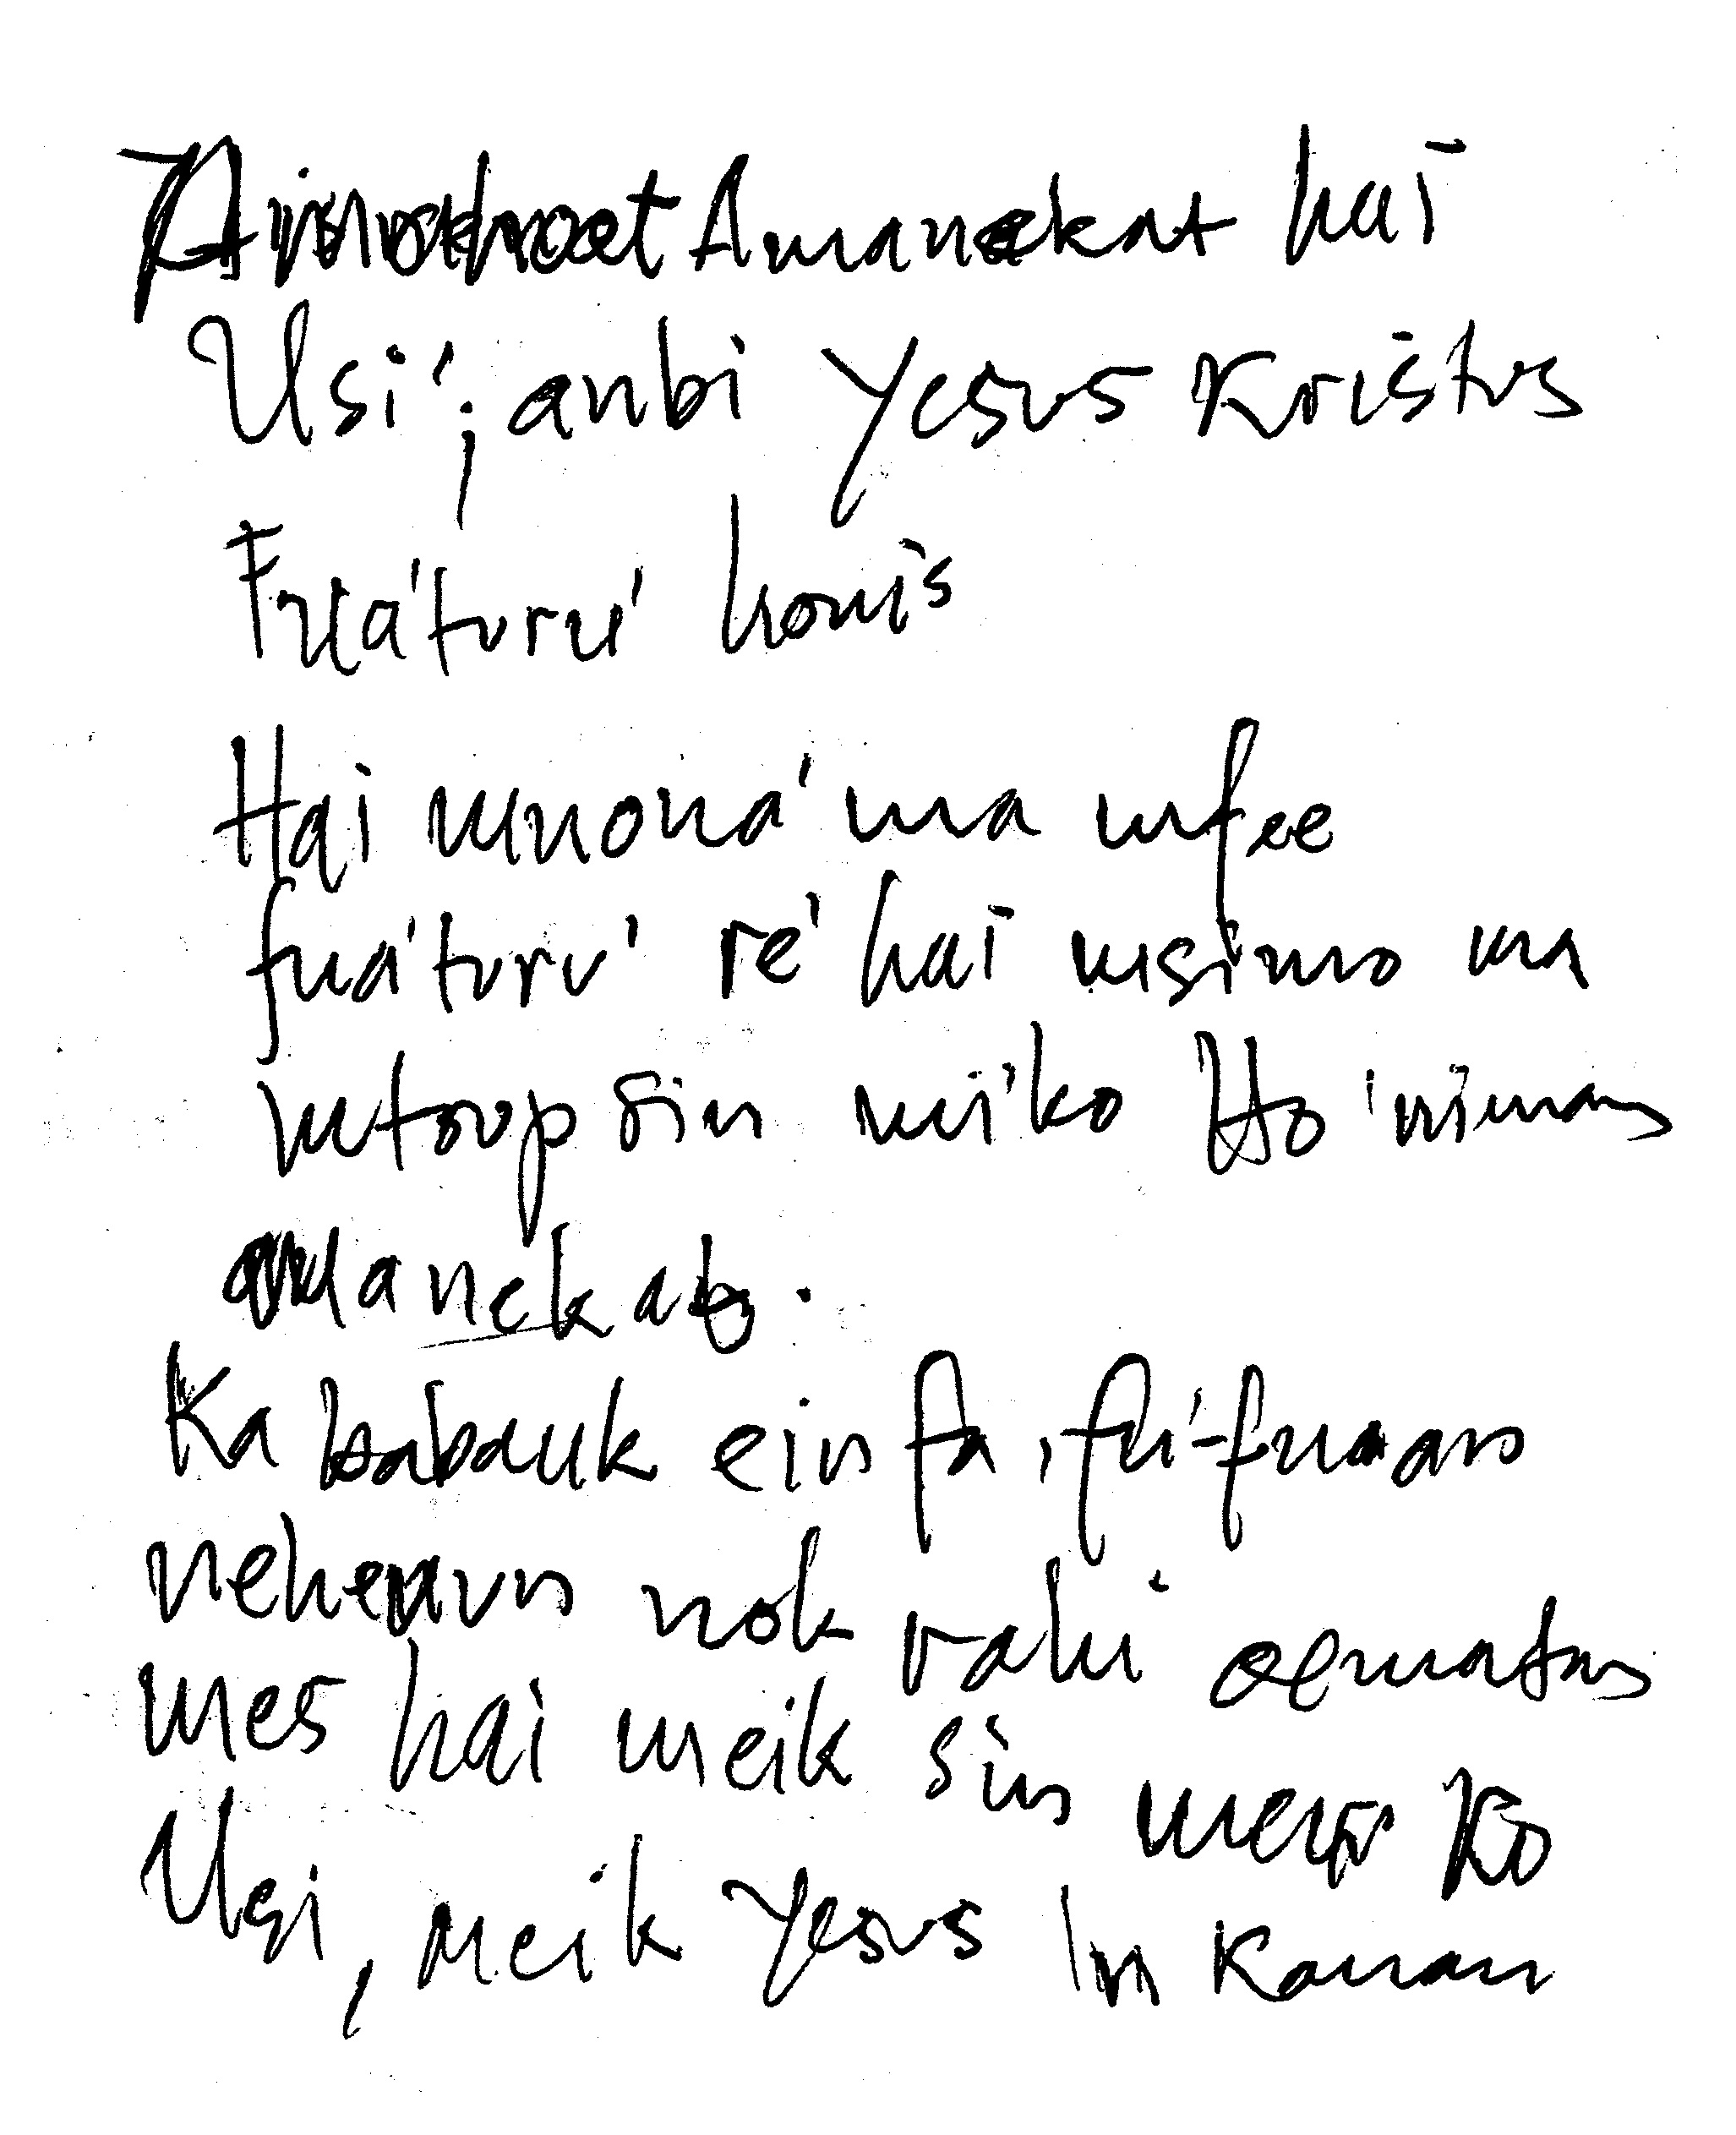
\includegraphics[width=0.6\columnwidth]{aaz-nodate-OffertoryPrayer.jpg}}
\end{figure}

A third example of parallel verbs with an alternate U\=/form and M\=/form
is given in \qf{ex:130825-3, 1.15-1.21}.
In this case the doublet is \ve{tenu \tcb{‖} hafo} `umbrella : shade'.

\newpage
\begin{exe}
	\ex{Speech to welcome new government officials:
				\txrf{130825-3} {\emb{130825-3-01-15-01-21.mp3}{\spk{}}{\apl}}}\label{ex:130825-3, 1.15-1.21}
	\begin{xlist}
		\ex{\glll	hai mi-ʔpiruʔ =kii ʔpiur suun mees nua\\
							hai mi-ʔpiruʔ =kii ʔpiruʔ suna meseʔ nua\\
							{\hai} {\mi}-cloth{\Uc} ={\kii} cloth horn single two\\
				\glt	`We give you two single bandannas (as a) horn' \txrf{1.15}}\vspace{4pt}
		\ex{\glll	henatiʔ \bxA{m-te\tbr{nu}} =m \bxB{mu-ha\tbr{of}} too{\gap}tafaʔ =kai {\lks}\\
							henatiʔ {\gp}m-tenu =ma {\gp}mu-hafo too{\gap}tafaʔ =kai\\
							{\he} \gp\m-umbrella{\tbrU} =and \gp\muu-shade{\tbrM} citizen ={\kai}\\
				\glt	`so that you might shade [doublet] us people.' \txrf{1.21}}
	\end{xlist}
\end{exe}

The two main patterns in which an Amarasi poetic doublet
of parallel verbs occur are given
in \qf{ex:AmaParVerPai} and \qf{ex:AmaParVerPai2} below.

\begin{exe}
	\ex{\xytext{\fbox{verb\sub{1}{\M}}\xybarconnect[2][-]{2}&and&\fbox{verb\sub{2}{\M}}}}\label{ex:AmaParVerPai}
	\ex{\xytext{\fbox{verb\sub{1}{\U}}\xybarconnect[2][-]{2}&and&\fbox{verb\sub{2}{\M}}}}\label{ex:AmaParVerPai2}
\end{exe}

In non-poetic discourse the use of a U\=/form followed by \ve{=ma}
indicates that the event marked by the U\=/form preceded the
event encoded in the next clause, as discussed in \srf{sec:Coo=Ma}.
However, in poetry such U\=/forms do not indicate the timing of events.
Instead, the use of U\=/forms and M\=/forms is a poetic device,
providing the option of a double parallelism on complementary verbs;
such verbs are both semantically and morphologically parallel.

\section{Centre of chiasmus}\label{sec:CenChi}
Another use of discourse U-forms is to mark the centre of a chiasmus.
Chiasmus is a kind of inverted parallelism in which parallel pairs
are repeated on either side of another parallel pair.
A simple example of chiasmus in English is given in \qf{ex:Macbeth}
below from act 1, scene 1 of Shakespeare's Macbeth.

\begin{exe}
	\ex{\it{\xytext{\fbox{Fair\vp{f}}\xybarconnect[4][-]{6}&is&\fbox{\,foul}\xybarconnect[2][-]{2}&and&\fbox{\,foul}&is&\fbox{\,fair.}}}}\label{ex:Macbeth}
\end{exe}

In Amarasi a U-form can occur in the middle of chiasmus to signal
that the information before this U-form
is going to be repeated again as illustrated in \qf{ex:ChiUfor} and \qf{ex:ChiUfor2} below.
There are 20 examples of U-forms marking chiasmus in my corpus.

\begin{exe}
	\ex{Chiastic U-forms:}\label{ex:ChiUfor}
		\begin{xlist}
			\exi{A.}{information\sub{1}}
			\sn{B. verb{\U}}
			\exi{A.}{information\sub{1}}
		\end{xlist}
\end{exe}

\begin{exe}
	\ex{\xytext{\fbox{information\sub{1}\vp{|}}\xybarconnect[2][-](D,D){2}\xybarconnect[2][<-]{1}&\fbox{U-form\vp{|}}\xybarconnect[2][->]{1}&\fbox{information\sub{1}\vp{|}}}}\label{ex:ChiUfor2}
\end{exe}

By using a U-form in such examples the speaker
signals non-resolution and puts the listener
in a mild state of suspense, communicating
roughly `This is unresolved. Pay attention'.
The listener would thus be prepared for something unexpected.
By repeating old information
instead of providing something new,
the speaker emphasises this repeated information.
The U-form is resolved by the information on either side of it.

At its most simple, such U-forms are preceded and followed
by an identical word or phrase.
This simple chiastic structure constitutes nearly all
instances of chiasmus with a central U-form in my corpus (18/20 instances).
One example is given \qf{ex:130925-1, 4.10} below,
in which the U-form \ve{n-moni} `lives' is both preceded and followed
by M-forms of the verb \ve{n-boʔis} `praises'.

\begin{exe}
	\ex{\xytext{\fbox{praise{\Mv}\vp{|}}\xybarconnect[2][-](D,D){2}\xybarconnect[2][<-]{1}&\fbox{live{\U}\vp{|}}\xybarconnect[2][->]{1}&\fbox{praise{\Mv}\vp{|}}}}
	\sn{\glll	\tbr{n}-\tbr{boiʔs}=\tbr{ee} mate-s. aam baab-f=ee n-\tbr{moni} =te, \tbr{n}-\tbr{boiʔs}=\tbr{ee}. \tcb{???\footnotemark}\\
						n-boʔis=ee mate-s ama baba-f=ee n-moni =te n-boʔis=ee\\
						\n-praise={\eeV} die-{\at} father FZ/MB-{\F}={\ee} \n-live{\tbrU} ={\te} \n-praise={\eeV}\\
			\glt	`He praised him a lot (\emph{lit.} dead). While the uncle was alive, he praised him.'
						\txrf{130925-1, 4.10} {\emb{130925-1-04-10.mp3}{\spk{}}{\apl}}}\label{ex:130925-1, 4.10}
\end{exe}
\footnotetext{
		The final word/phrase of this sentence
		was not transcribed by Roni,
		who recorded and transcribed this text.
		Due to the faintness of the recording,
		I also cannot make out the final word/phrase of this sentence.
		My best guess is that it is \ve{na-hiin\j=ee} `he knew it/him'.}

A more complex example is given in \qf{ex:120923-2-, 4.29-4.34} below,
in which the material which surrounds the U-form
is repeated multiple times, including two repetitions
which are not identical but parallel.
The structure of this chiasmus is given in \qf{ex:Chi ex:120923-2-, 4.29-4.34} below.

\begin{exe}
	\ex{Chiasmus of \qf{ex:120923-2-, 4.29-4.34}:}\label{ex:Chi ex:120923-2-, 4.29-4.34}
		\begin{xlist}
			\exi{A.}{\ve{na-pein=koo} = `gets you'}
			\exi{A.}{\ve{na-pein=koo} = `gets you'}
			\sn{\lh{A′.} B. \ve{t-soʔi} = `counts{\U}'}
			\sn{A′. \ve{n-naaʔ=koo} = `holds you'}
			\sn{A′. \ve{n-naaʔ=koo} = `holds you'}
			\exi{A.}{\ve{na-pein=koo} = `gets you'}
		\end{xlist}
\end{exe}

\begin{exe}
	\ex{Catching a thief in your garden: \txrf{120923-2} {\emb{120923-2-04-29-04-34.mp3}{\spk{}}{\apl}}}\label{ex:120923-2-, 4.29-4.34}
	\sn{\xytext{\fbox{gets you\vp{h}}\xybarconnect[4][-]{1}\xybarconnect[2][-](D,D){1}&\fbox{gets you\vp{h}}\xybarconnect[4][-]{4}\xybarconnect[2][-](D,D){2}&counts{\U}&\fbox{holds you}\xybarconnect[2][-]{1}&\fbox{holds you}\xybarconnect[2][-](D,D){1}&\fbox{gets you\vp{h}}}}
		\begin{xlist}
			\ex{\glll	\sf{karna} tuan=ee \tbr{na}-\tbr{pein} =\tbr{koo}, \tbr{na}-\tbr{pein} =\tbr{koo} naa\j=ena =ma\\
								\sf{karna} tuan=ee na-peni =koo na-peni =koo nai=ena =ma\\
								because owner={\ee} \na-get{\M} ={\koo} \na-get{\M} ={\koo} already={\een} =and\\
					\glt	`Because the owner gets you, he's got you already and' \txrf{4.29}}
			\ex{\glll	t-so\tbr{ʔi} =t iin n-naaʔ =koo,\\
								t-soʔi =te ini n-naʔa =koo\\
								\tg-count{\tbrU} ={\te} {\iin} \n-hold{\M} ={\koo}\\
					\glt	`(someone) counts while he holds you' \txrf{4.32}}
			\ex{\glll	{n}-{naaʔ} ={koo} na-heer=een ees reʔ \hspace{40mm} iin {na}-{pein} ={koo} reʔ ia.\\
								n-naʔa =koo na-hera=ena esa reʔ {} ini na-peni =koo reʔ ia\\
								\n-hold{\M} ={\koo} \na-tight={\een} one {\req} {} {\iin} \na-get{\M} ={\koo} {\req} {\ia}\\
					\glt	`He holds you tight like this, the one who's got you here.' \txrf{4.34}}
	\end{xlist}
\end{exe}

The U-forms in examples \qf{ex:130925-1, 4.10} and \qf{ex:120923-2-, 4.29-4.34}
have a dual function, marking both the chiasmus
as well as dependent coordination (\srf{sec:DepCoo}).
In these cases the information which resolves the U-form is similar/identical
to that which precedes the U-form.

In addition to such examples in which there is only a single layer
on either side of the U-form,
there are at least two examples of a more complex chiastic structure
in which there is more than one layer surrounding the U-form,
as exemplified in \qf{ex:ComChi} and \qf{ex:ComChi2} below.

\begin{exe}
	\ex{Complex Chiasmus:}\label{ex:ComChi}
		\begin{xlist}
			\exi{A.}{information\sub{1}}
			\sn{B. information\sub{2}}
			\sn{{\lh{B. }}C. verb{\U}}
			\sn{B. information\sub{2}}
			\exi{A.}{information\sub{1}}
		\end{xlist}
	\ex{\xytext{\fbox{information\sub{1}}\xybarconnect[4][-](D,D){4}\xybarconnect[4][<-]{2}&\fbox{information\sub{2}}
							\xybarconnect[2][-](D,D){2}\xybarconnect[2][<-](U,UL){1}&\fbox{verb{\U}\vp{|}}\xybarconnect[2][->](UR,U){1}\xybarconnect[4][->]{2}&\fbox{information\sub{2}}&
							\fbox{information\sub{1}}}}\label{ex:ComChi2}
\end{exe}

The first of these examples is given in \qf{ex:130825-6, 2.57-3.01} below.
This example consists of an outer layer (`I just followed the target.')
an inner layer (`I couldn't offer') with the core U-form \ve{ʔ-nesi} `more'.
The chiastic structure of \qf{ex:130825-6, 2.57-3.01} is given in \qf{ex:Chi ex:130825-6, 2.57-3.01}.


\begin{exe}
	\ex{Chiasmus in \qf{ex:130825-6, 2.57-3.01}:}\label{ex:Chi ex:130825-6, 2.57-3.01}
		\begin{xlist}
			\exi{A.}{\it{I just followed the target}}
			\sn{B. \it{I couldn't offer}}
			\sn{\lh{B. }C. \it{any more}{\U}}
			\sn{B. \it{I couldn't offer}}
			\exi{A.}{\it{I just followed the target}}
		\end{xlist}
\end{exe}

\begin{exe}
	\ex{Donating money: \txrf{130825-6} {\emb{130825-6-02-57-03-01.mp3}{\spk{}}{\apl}}}\label{ex:130825-6, 2.57-3.01}
		\begin{xlist}
			\ex{\gll	au ʔ-tuin=aah neʔ \sf{target}.\\
								{\au} \q-follow=just {\reqt} target\\
					\glt	`I just followed the target.' \txrf{}}
			\ex{\glll	au ka= bisa ʔ-\sf{korban} a|ʔ-\tbr{nesi} =f.\\
								au ka= bisa ʔ-\sf{korban} {\a}ʔ-nesi =fa\\
								{\au} {\ka}= can \q-sacrifice {\a\q}-more{\tbrU} ={\fa}\\
					\glt	`I couldn't offer any more.' \txrf{2.57}}
			\ex{\gll	au ka= bisa ʔ-\sf{korban}.\\
								{\au} {\ka}= can \q-sacrifice \\
					\glt	`I couldn't offer.' \txrf{}}
			\ex{\gll	au ʔ-tuin=aah neʔ \sf{target}.\\
								{\au} \q-follow=just {\reqt} target\\
					\glt	`I just followed the target.' \txrf{3.01}}
	\end{xlist}
\end{exe}

A second example is given in \qf{ex:130825-6, 9.20-9.28} below,
with the chiastic structure summarised in \qf{ex:Chi ex:130825-6, 9.20-9.28}.
In this example the outer layer consists of the person \ve{Olpi}
the inner layer consists of the activity `went down to bathe'
and the U-form in the centre in \qf{ex:130825-6, 9.20b} is \ve{n-sae n-fani} `came back up'.
This core is also followed by an additional event in \qf{ex:130825-6, 9.20-9.28}.

\begin{exe}
	\ex{Chiasmus in \qf{ex:130825-6, 9.20-9.28}:}\label{ex:Chi ex:130825-6, 9.20-9.28}
		\begin{xlist}
			\exi{A.}{\it{Olpi}}
			\sn{B. \it{went down to bathe}}
			\sn{\lh{B. }C. \it{came back}{\U} \it{up}}
			\sn{\lh{B. }D. \it{handed me a towel and soap}}
			\sn{B. \it{I went down to bathe}}
			\exi{A.}{\it{Olpi}}
		\end{xlist}
\end{exe}

\begin{exe}
	\ex{The narrator and Olpi are down at the garden:\txrf{130825-6} {\emb{130825-6-09-20-09-28.mp3}{\spk{}}{\apl}}}\label{ex:130825-6, 9.20-9.28}
		\begin{xlist}
		\ex{\glll	Olpi n-saun na-niu =ma nsa--,\\
							Olpi n-sanu na-niu =ma\\
							Olpi \n-go.down{\M} \na-bathe =and\\
				\glt	`Olpi went down to bathe and' \txrf{9.20}}
		\ex{\glll	n-sae n-\tbr{fani} =t\\
							n-sae n-fani =te\\
							\n-go.up \n-back{\tbrU} ={\te}\\
				\glt	`when he came back up,' \txrf{9.22}}\label{ex:130825-6, 9.20b}
		\ex{\glll	n-nonaʔ =kau nehh, n-nonaʔ =kau nehh, \sf{handuk} =am \sf{sabu} \\
							n-nonaʔ =kau {} n-nonaʔ =kau {} \sf{handuk} =ma \sf{sabu} \\
							{\n}-hand ={\kau} {} {\n}-hand ={\kau} {} towel =and soap \\
				he handed me handed me  a towel and soap.' \txrf{9.23}}\label{ex:130825-6, 9.20}
		\ex{\glll	ʔ-saun u-niu =t, \\
							ʔ-sanu u-niu =te \\
							{\q}-go.down{\M} {\qu}-bathe ={\te}\\
				\glt `I went down and bathed while' \txrf{9.27}}
		\ex{\glll	Olpi n-ait nehh, hap-- hapee\j=ii \\
							Olpi n-aiti {} {} hapei=ii \\
							Olpi {\n}-pick.up{\M} {} {} mobile.phone={\ii} \\
				\glt `Olpi picked up the mobile phone' \txrf{9.28}}
	\end{xlist}
\end{exe}

U-forms can mark the centre of a chiasmus.
By introducing a U-form the narrator
sets up the discourse as unresolved and introduces
the possibility of an unexpected event.
By then denying this possibility and
repeating the information which occurred before the U-form,
the narrator emphasises the repeated information.
A U-form in the centre of chiasmus is resolved by
the information on either side of it.

\section{Interactional metathesis alternations}\label{sec:IntUnm}
Another use of discourse U-forms is in conversation
to maintain interaction between speakers.
By using a U-form in conversation, the speaker flags
that s/he considers the communicative act unresolved.
This provides an opportunity for other participants
to make their own contribution and resolve the U-form.
In my corpus there are 53 instances of U-forms
which are intended to elicit a response from the addressee.
This frequency is discussed in more detail in \srf{sec:FreUfoCon}.

\subsection{Question and answer}\label{sec:Q/A}
The clearest example of U-forms being used in
interactions between speakers is in question-answer pairs.
U-forms are used to ask questions and M-forms
are used to answer such questions.
The normal structure of an Amarasi question-answer pair is given in \qf{ex:Q/A} below.
The question and answer usually contain identical verbs,
with the question U-form being resolved by an M-form answer.
A typical example is given in \qf{ex:02/08/13, p.20}.
Here, and throughout this section, Greek letters
are used to mark different speakers.

\begin{exe}
	\ex{\xytext{Speaker\sub{1}:&\fbox{U-form}\xybarconnect[2][-](D,D){2}\xybarconnect[2][->]{2}&Speaker\sub{2}:&\fbox{M-form}}}\label{ex:Q/A}
\end{exe}

\begin{multicols}{2}
	\begin{exe}
		\ex{Climbing a steep hill:}\label{ex:02/08/13, p.20}
			\begin{xlist}
				\ex[α:]{\gll	hoo mu-be\tbr{ʔi}?\\
									%	hoo mu-beʔi\\
									{\hoo} \mu-capable{\U}\\
						\glt	`Can you do it?'}
			\end{xlist}
		\sn{ \txrf{observation 02/08/13, p.20}}
			\begin{xlist}
				\exi{b.}[β:]{\gll	au u-be\tbr{iʔ}!\\
									%	au u-beʔi\\
									{\au} \qu-capable{\tbrM}\\
						\glt	`Yes, I can!'}
			\end{xlist}
	\end{exe}
\end{multicols}

Such question-answer pairs are similar to tail-head linkage (\srf{sec:TaiHeaLin})
or poetic parallelism (\srf{sec:PoePar}) with the difference
that the U-form/M-form doublet is constructed by multiple speakers.
U-form questions must be complemented by an M-form answer
and U-form answers are judged as infelicitous.
This is shown in (\ref{ex:02/08/13, p.20}′) below,
which can be compared with grammatical \qf{ex:02/08/13, p.20} above.

\begin{multicols}{2}
	\begin{exe}
		\exp{ex:02/08/13, p.20}{Elicitation:\label{ex:03/10/14 p.112}}
			\begin{xlist}
				\ex{\gll	hoo mu-beʔi?\\
									%	hoo mu-beʔi\\
									{\hoo} \mu-capable{\U}\\
						\glt	`Can you do it?'}
			\end{xlist}
		\sn{\txrf{el. 03/10/14 p.112}}
			\begin{xlist}
				\exi{b.}[{\#}]{\gll	au u-beʔi\\
									%	au u-beʔi\\
									{\au} \qu-capable{\U}\\
						\glt	`Yes, I can!'}
			\end{xlist}
	\end{exe}
\end{multicols}

Two examples of question{\U}-answer{\M} pairs from recorded
conversations are given in \qf{ex:130914-1, 0.20-0.21}
and \qf{ex:130909-6, 3.23-3.25} below.
In each example a question posed in the U-form is answered
by another speaker with an M-form version of the same verb.

\begin{exe}
	\ex{Weaving cloth: \txrf{130914-1} {\emb{130914-1-00-20-00-21.mp3}{\spk{}}{\apl}}}\label{ex:130914-1, 0.20-0.21}
		\begin{xlist}
			\ex[α:]{\glll	he t-fu\tbr{tu}?\\
										he t-futu\\
										{\he} \t-bind{\tbrU}\\
							\glt	`Should we tie it?' \txrf{0.20}}
			\ex[β:]{\glll	t-fu\tbr{ut}, reʔ mutiʔ reʔ ia.\\
										t-futu reʔ mutiʔ reʔ ia\\
										\t-bind{\tbrM} {\req} white {\req} {\ia}\\
							\glt	`(Yes,) we tie it. The white one which is here.' \txrf{0.21}}
		\end{xlist}
	\ex{Inquiring about family: \txrf{130909-6} {\emb{130909-6-03-23-03-25.mp3}{\spk{}}{\apl}}}\label{ex:130909-6, 3.23-3.25}
		\begin{xlist}
		\ex[α:]{\glll	ehh, n-fain=n=ena? naiʔ Rius iin\j=ana n-fa\tbr{ni}?\\
									{} n-fani=n=ena naiʔ Rius ini=ana n-fani\\
									{} \n-back{\Mv}=\einV={\een} {\naiq} Lius {\iin}={\aan} \a\n-back{\tbrU}\\
						\glt	`Ahh, they've come back, right? Lius's (child) has come back?' \txrf{3.23}}
		\ex[β:]{\glll	iin n-fa\tbr{in}, tua.\\
									ini n-fani tua\\
									{\iin} \n-back{\tbrM} {\tua}\\
						\glt	`He's come back.' \txrf{3.25}}
		\end{xlist}
\end{exe}

However, it is not a rule of Amarasi grammar that
questions \it{must} be posed in the U-form.
Two examples of questions posed in the M-form
are given in \qf{ex:130825-1.28-1.31} and \qf{ex:130913-1, 0.57-0.59 ch:DisMet} below.
In each example the M-form question also
elicits a response (partially) in the M-form.

\begin{exe}
	\ex{Going to Jakarta: \txrf{130825-7} {\emb{130825-7-01-28-01-31.mp3}{\spk{}}{\apl}}}\label{ex:130825-1.28-1.31}
		\begin{xlist}
			\ex[α:]{\glll	n-moaʔ on mee =m esa n-heek n-a\tbr{an} =koo n-ok bifee? \sf{atau,} aiʔ hoo m-mo\tbr{uf}?\\
										n-moʔe on mee =ma esa n-heke n-ana =koo n-oka bifee \sf{atau} aiʔ hoo m-mofu\\
										\n-do{\M} like how =and {\es} \a\n-catch{\M} \n-{\ana}{\tbrM} ={\koo} \n-{\ok\M} woman or or {\hoo} \m-fall{\tbrM}\\
							\glt	`How did it happen, that is did they catch you with the woman? Or did you fall (morally)?' \txrf{1.28}}
			\ex[β:]{\glll	ka= n-he\tbr{ek} =kau =f!\\
										ka= n-heke =kau =fa\\
										{\ka}= \n-catch{\tbrM} ={\kau} ={\fa}\\
							\glt	`They didn't catch me!' \txrf{1.31}}
		\end{xlist}
	\ex{A man who's already made preparations for his funeral:
				\txrf{130913-1} {\emb{130913-1-00-57-00-59.mp3}{\spk{}}{\apl}}}\label{ex:130913-1, 0.57-0.59 ch:DisMet}
			\begin{xlist}
				\ex[α:]{\glll	m-ak iin n-hain n-me\tbr{es}?\\
											m-ak ini n-hani n-mese\\
											\m-say {\iin} \n-dig{\M} \n-alone{\tbrM}\\
								\glt	`Do you think he dug it alone?' \txrf{0.57}}
				\ex[β:]{\glll	iin ofa n-hani n-me\tbr{es}.\\
											ini ofa n-hani n-mese\\
											{\iin} sure \n-dig{\Uc} \n-alone{\tbrM}\\
								\glt	`He must've dug it himself.' \txrf{0.59}}
			\end{xlist}
\end{exe}

A useful tool for analysing U-form/M-form question-answer pairs in Amarasi
is provided by the notion of an \emph{adjacency pair},
a concept developed by \citet[295]{scsa77} within the field of conversation analysis.
An adjacency pair has the following properties:

\begin{exe}
	\ex{An adjacency pair: \txrf{}}\label{ex:AnAdjPai}
	\begin{xlist}
		\ex{consists of two conversational turns:}
			\begin{xlist}
				\ex{which are by different speakers}\label{ex:AnAdjPai-1}
				\ex{which are placed next to one another}\label{ex:AnAdjPai-2}
				\ex{which are ordered}\label{ex:AnAdjPai-3}
				\ex{which are differentiated into pair types}\label{ex:AnAdjPai-4}
			\end{xlist}
	\end{xlist}
\end{exe}

The first part of an adjacency pair
is known as the \emph{first pair part}
and the second part is called the \emph{second pair part}.
Property \qf{ex:AnAdjPai-3} refers to the fact
that these two pairs come in a set order:
i.e. a question (first pair part) precedes an answer (second pair part).
Property \qf{ex:AnAdjPai-4} refers to
the fact that which second pair part is allowed
is constrained by the first pair part.
An acceptable second pair part for a greeting
is another greeting, while an acceptable
second pair part for a question is an answer.

The Amarasi examples seen so far in this section
are question-answer adjacency pairs.
U-forms occur as first pair parts (questions)
and M-forms occur in second pair parts (answers).

A first pair part projects the relevant second pair part.
If the relevant second pair part is lacking,
the conversation is viewed as problematic or incomplete.
Thus, for instance when a speaker asks a question,
they expect to receive an answer.
This is illustrated with the English example in \qf{ex:ACon} below,
taken from \cite{li07} with the transcription adapted to the same
transcription conventions used in this book.

\begin{exe}
	\ex{A conversation: \hfill\cite[108]{li07}}\label{ex:ACon}
	\begin{xlist}
		\ex[α:]{\it{Did you speak to Mary today?}}\label{ex:ACon-1}
		\ex[\hp{α:}]{{[}0.2 seconds of silence{]}}\label{ex:ACon-2}
		\ex[α:]{\it{Did you speak to Mary?}}\label{ex:ACon-3}
		\ex[β:]{\it{Oh, yeah I saw her at lunch.}}\label{ex:ACon-4}
	\end{xlist}
\end{exe}

In \qf{ex:ACon-1} speaker-α's question is followed by 0.2 seconds of silence,
which is interpreted by speaker-α as the answer being absent,
as a result s/he repeats the question in \qf{ex:ACon-3}
which induces the required answer in \qf{ex:ACon-4}.

Within the terminology of conversation analysis,
a U-form in Amarasi explicitly flags a turn as
the first pair part of a question-answer adjacency pair.\footnote{
		An interesting topic to pursue for further work
		would be whether questions posed in the M-form
		do not require an answer in the same way as those posed in the M-form.
		It may be the case that U-forms questions are first pair parts
		while M-form questions are not}
This thus projects forward an answer as the second pair part.
Within more general terminology,
U-forms are one way of marking a question
which expects an explicit answer.
Such U-form questions are complemented and completed by an M-form answer.

\subsection{Maintaining interaction}\label{sec:MaiInt}
U-forms are not only used in questions.
but are used more broadly to maintain
ongoing interaction and conversation between speakers.
One example is given in \qf{ex:19/09/14 p.97} below.
In this example speaker-α wants to interact with speaker-β.
Speaker-α initiates a conversation in \qf{ex:19/09/14 p.97-1} and
speaker-β responds with the M-form \ve{ʔ-took} `sit' in \qf{ex:19/09/14 p.97-2}.
Speaker-α then repeats this answer with a U-form \ve{m-toko} `sit' in \qf{ex:19/09/14 p.97-3}.
By using a U-form in \qf{ex:19/09/14 p.97-3} speaker-α
signals that the interaction is not yet socially complete.
When speaker-β fails to resolve the U-form,
speaker-α does so himself by offering betel nut
in \qf{ex:19/09/14 p.97-4}, the chewing of which is
a core Timorese social activity.

\begin{exe}
	\ex{Speaker-α approaches speaker-β and friends: \txrf{observation 19/09/14 p.97}}\label{ex:19/09/14 p.97}
		\begin{xlist}
			\ex[α:]{\glll	hoo mu-nsaaʔ? \\
										hoo mu-nsaaʔ \\
								 {\hoo} \mu-do.what\\
					\glt `What are you doing?'}\label{ex:19/09/14 p.97-1}
			\ex[β:]{\glll	au ʔ-to\tbr{ok}. \\
										au ʔ-toko \\
										{\au} {\q}-sit{\tbrM} \\
							\glt `I'm sitting.'}\label{ex:19/09/14 p.97-2}
			\ex[α:]{\gll	hoo m-to\tbr{ko}? \\
								 {\hoo} {\m}-sit{\tbrU}\\
					\glt `So, you're sitting, are you?'}\label{ex:19/09/14 p.97-3}
			\ex[α:]{\emph{[approaches group and offers betel nut]}}\label{ex:19/09/14 p.97-4}
		\end{xlist}
\end{exe}

A similar example is given in \qf{ex2:19/09/14 p.97} below.
In \qf{ex2:19/09/14 p.97-1} speaker-β
invites speaker-α to go first at a buffet.
This invitation is accepted by speaker-α
in \qf{ex2:19/09/14 p.97-2} with the U-form \ve{u-hunu} `first';
this is a kind of rhetorical question casting.
This U-form is then resolved by speaker-β
nodding that this is indeed the intended desire.
%Both examples \qf{ex:19/09/2014 p.97} and \qf{ex2:19/09/2014 p.97}
%exhibit an M-form followed by a U-form,
%the same pattern seen in head-tail linkage (\srf{sec:HeaTaiLin}).

\begin{exe}
	\ex{Lining up at a buffet to get food: \txrf{observation 19/09/14 p.97}}\label{ex2:19/09/14 p.97}
	\begin{xlist}
		\ex[β:]{\glll	hoo mu-hu\tbr{un}. \\
									hoo mu-hunu \\
							 {\hoo} \mu-first{\tbrM}\\
				\glt `You go first.' \emph{[simultaneously gestures with hands]}}\label{ex2:19/09/14 p.97-1}
		\ex[α:]{\gll	au u-hu\tbr{nu}.\\
									{\au} {\qu}-first{\tbrU}\\
						\glt `I'll go first, then?'}\label{ex2:19/09/14 p.97-2}
		\ex[β:]{\emph{[nods once and gestures]}}
		\ex[α:]{\emph{[starts serving food]}}
	\end{xlist}
\end{exe}

A number of more complex interactional U-forms are given
in \qf{ex:130825-7, 3.30-3.35}--\qf{ex:130909-6, 1.12-1.26}.
In \qf{ex:130825-7, 3.30-3.35} a group of speakers are discussing what
to do about the presence of a voice recorder.
Speaker-β announces in \qf{ex:130825-7, 3.33} his intention
with a U-form \ve{ʔ-nene} `press'.
This verb is then repeated in the M-form by speaker-α who
points out that speaker-β is not achieving his goal.
The U-form is not resolved by the action,
but it is resolved by the interaction.

\begin{exe}
	\ex{Turning a voice recorder off: \txrf{130825-7} {\emb{130825-7-03-30-03-40.mp3}{\spk{}}{\apl}}}\label{ex:130825-7, 3.30-3.35}
	\begin{xlist}
		\ex[α:]{\gll	t-\sf{sambuŋ} peo-t=ee, he bisa bees\j=ee na-taah =kiit.\\
									\t-continue talk-\at={\ee} {\he} can machine={\ee} {\na}-answer ={\kiit}\\
						\glt	`(If) we keep talking the machine will be able to answer us.' \txrf{3.30}}
		\ex[β:]{\glll	maut he au ʔ-ne\tbr{ne}!\\
									maut he au ʔ-nene\\
									patient {\he} {\au} \q-press{\tbrU}\\
						\glt	`Hold on, I'll press (the buttons)!' \txrf{3.33}}\label{ex:130825-7, 3.33}
		\ex[α:]{\ve{Aeʔ!} \\
								`Hey!' \txrf{3.34}}
		\ex[β:]{\emph{[laughs]}}
		\ex[α:]{\glll	maan m-ne\tbr{en} mu-tafiʔ bees\j=ee naan, kamaʔ. Hoe! \sf{Australi} \sf{puɲa} \sf{ini.}\\
									maan m-nene mu-tafiʔ besi naan kamaʔ hoe \sf{Australi} \sf{puɲa} \sf{ini}\\
									like.that \m-press{\tbrM} \mu-random{\Uc} machine{\U} {\naan} what's-it hey Australia have this\\
						\glt	`You're randomly pressing the machine there, (that) what's-it. Hey! This belongs to Australia.' \txrf{3.35}}
		\ex[α:]{\gll	hoo m-ak besi kraufn=ees, ees reʔ naan on reʔ \sf{hapei}=ein reʔ a-taf{\tl}taifʔ=ein.\\
									{\hoo} \m-say machine useless={\es} one {\req} {\naan} like {\reqt} mobile.phone={\ein} {\req} {\at}-{\prd}agape={\ein}\\
						\glt	`You think it's a useless machine, the one there, like those mobile phones which leave you agape (with confusion).' \txrf{3.40}}
	\end{xlist}
\end{exe}

Example \qf{ex:130911-2, 0.30-0.39} below involves a number of U-forms.
None of these \mbox{U-forms} is repeated by another speaker,
but in each instance a U-form is followed by the contribution of another speaker.
By using U-forms, the speakers indicate that they
do not consider the communicative act resolved
and thereby open the floor up for 
contributions from other speakers.
The only change of speaker in \qf{ex:130911-2, 0.30-0.39} which does
not involve a U-form is that after \qf{ex:130911-2, 0.30}
in which \qf{ex:130911-2, 0.32} is an interruption 
cutting off the first speaker mid sentence.

\begin{exe}
	\ex{A conversation about a car which came off the road:
			\txrf{130911-2} {\emb{130911-2-00-31-00-40.mp3}{\spk{}}{\apl}}}\label{ex:130911-2, 0.30-0.39}
	\begin{xlist}
		\ex[α:]{\gll	iin na-reen=oo-n =ma n-\sf{ʔantareek} a|n-bi n-- \\
									{\iin} \na-force{\Mv}={\oo=\N} =and \n-backing \a\n-{\bi} {}\\
						\glt `He forced himself, and went back into it, was in{\ldots}' \txrf{0.31}}\label{ex:130911-2, 0.30}
		\ex[β:]{\gll	na-ba\tbr{ra} maʔbakeʔ mhh.\\
									 {\na}-forever{\tbrU} narrow {}\\
						\glt `He was stuck in the narrow (place)' \txrf{0.32}}\label{ex:130911-2, 0.32}
		\ex[γ:]{\gll	iin he n-bi\tbr{bi}. \\
									 {\iin} {\he} {\n}-shrink{\tbrU}\\
						\glt `He would've wanted to shrink (the car).' \txrf{0.34}}
		\ex[δ:]{\gll n-ak, ootgw=ii, na-snii m-ak, =am, na-kamaf =am,\\
									\n-say car={\ii} \na-slope \m-say and \na-what's.it{\Uc} =and\\
						\glt `he said, the car was sloping, you think, and what's it and' \txrf{0.35}}
		\ex[]{\glll na-snii n-taikobi n-koon, naʔ na-te\tbr{tu}\\
									na-snii n-taikobi n-kono naʔ na-tetu\\
									\na-slope \n-fall{\Uc} \n-keep.on{\M} then \nat-upright{\tbrU}\\
						\glt `it was sloping, fell over, kept on and only then he got the car upright' \txrf{0.38}}
		\ex[β:]{\gll	{onai =ma}  srutun reʔ ia, iin n-moofgw=een. \\
									and.so suddenly {\req} {\ia} {\iin} \n-fall{\Mv}={\een} \\
				\glt `and suddenly now it fell down' \txrf{0.40}}
	\end{xlist}
\end{exe}

A similar example of U-forms initiating a change of speakers
is given in \qf{ex:130909-6, 1.12-1.26},
which only involves two speakers.
In this example the change of speakers
after each of the following claues is initiated by a U-form:
\qf{ex:130909-6, 1.15}, \qf{ex:130909-6, 1.16}, and \qf{ex:130909-6, 1.22}.
This conversation also involves a large amount of repetition,
a discourse structure already noted in \srf{sec:DisStrAma}
as a feature of Amarasi monologues.

\begin{exe}
	\ex{Preparing a field for planting: \txrf{130909-6} {\emb{130909-6-01-12-01-26.mp3}{\spk{}}{\apl}}}\label{ex:130909-6, 1.12-1.26}
	\begin{xlist}
		\ex[α:]{\gll	mu-boor=een, ta-boor n-ok fuun ne\<ʔ\>e.\\
									\mu-make.hole={\een} \ta-make.hole \n-{\ok\M} moon six\<\qnum\>\\
						\glt	`You dug a hole. We dig holes (for planting) in June.' \txrf{1.12}}
		\ex[β:]{\glll	heʔ, t-ka\tbr{nu} =t, naʔ fuun ne\<ʔ\>e.\\
									{} t-kanu =te naʔ funan ne\<ʔ\>e\\
									hey \t-cut.field{\tbrU} ={\te} then moon six\<\qnum\>\\
						\glt	`What? We cut open a new field, only then is it June.' \txrf{1.15}}\label{ex:130909-6, 1.15}
		\ex[α:]{\glll	ehh,  t-ka\tbr{nu} =t, naʔ fuun ne\<ʔ\>e.\\
									{} t-kanu =te naʔ funan ne\<ʔ\>e\\
									oh \t-cut.field{\tbrU} ={\te} then moon six\<\qnum\>\\
						\glt	`Ohh{\ldots}, we cut open a new field, only then is it June.' \txrf{1.16}}\label{ex:130909-6, 1.16}
		\ex[β:]{\glll	t-tofa ʔteets=ii.\\
									t-tofa ʔtetas=ii\\
									\t-weed{\Uc} old.field={\ii}\\
						\glt	`We weed the old field..' \txrf{1.18}}\label{ex:130909-6, 1.18}
		\ex[α:]{\gll	t-toof n-ok fuun se\<ʔ\>o.\\
									\t-weed{\M} \n-{\ok\M} month{\M} nine\<{\qnum}\>\\
						\glt	`We weed (the field) in September.' \txrf{1.20}}
		\ex[β:]{\glll	hau, t-toof nai he n-me\tbr{to}, oo.\\
									hau t-tofa nai he n-meto oo\\
									yes \t-weed{\M} already he \n-dry{\tbrU} {\aaQ}\\
						\glt	`Yes, we weed (the field) after it's dried out, as you know.' \txrf{1.22}}\label{ex:130909-6, 1.22}
		\ex[α:]{\gll	neyahh, nean fauk=ii na-ʔuur?\\
								%	{} neno fauk=ii na-ʔura\\
									yeah day how.many={\ii} \na-rain{\M}\\
						\glt	`Yeah{\ldots} which day did it rain?' \txrf{1.26}}
	\end{xlist}
\end{exe}

U-forms can be used in conversation to maintain interaction
between speakers and to motivate a change of speaker.
By using a U-form, a speaker signals a lack of resolution
while other features such as intonation
and silence indicate that the speaker will not resolve the U-form.
It thus becomes incumbent on the addressee or audience
to provide a resolution to the U-form.

\subsection{Frequency of U-forms in conversation}\label{sec:FreUfoCon}
Discourse U-forms are nearly twice as frequent in conversations as in monologues in my corpus.
My Kotos Amarasi text collection consists of 182.49 minutes (three hours two minutes)
of recorded, transcribed and glossed texts.
Of this, 154.17 minutes (two hours thirty-four minutes)
are monologues: texts which consist mainly of a single speaker,
and 28.32 minutes (nearly half an hour) are conversations:
texts in which more than one person regularly speaks.

Of the 423 U-forms in my corpus which
cannot be explained by phonotactic constraints (\srf{sec:PhoCon}),
312 occur in monologues and 111 occur in conversations.
This gives a frequency rate of 2.02 discourse U-forms per minute in monologues
and 3.92 discourse U-forms per minute in conversations.
These figures are summarised in \trf{tab:VerUfoConMon}.

\begin{table}[h]
	\caption{Discourse U-forms in monologues and conversations}\label{tab:VerUfoConMon}
	\centering
		\begin{tabular}{rlll} \lsptoprule
															& Mon.	& Conv. & all			\\ \midrule
			total length (minutes)	& 154.17& 28.32	& 182.49	\\
			discourse U-forms				& 312		& 111		& 423			\\
			U-forms per minute			&	2.02	&	3.92	&	2.32		\\
			\lspbottomrule
		\end{tabular}
\end{table}

That discourse driven U-forms are nearly twice as frequent in conversations
than in monologues lends quantitative support to an analysis of U-forms
as being used interactionally by speakers in conversations
to motivate turn taking and change of speaker.

\subsection{Other interactional resources}\label{sec:OthIntRes}
U-forms are only one of several resources in Amarasi
available to speakers to maintain interaction with other speakers.
In this section I discuss the way a number of discourse particles
interact with discourse driven U-forms.

The addressee particle \ve{tua} is a polite way
in which a speaker can mark their contribution to the discourse as complete
Thus, it cannot co-occur with U-forms, which explicitly flag a lack of resolution.
On the other hand the question particles \ve{oo} and \ve{kaah}
require a response from the addressee.
Thus, they combine naturally with U-forms in direct questions.

\subsubsection{Addressee particle \it{tua}}\label{sec:AddParTua}
The addressee particle \ve{tua} cannot co-occur with interactional U-forms.
This is because such a U-form is unresolved or incomplete and
places an obligation on the addressee to respond to the speaker,
while \ve{tua} signals that the speaker considers their contribution complete.

The particle \ve{tua} is translated by native speakers as `yes' or `Sir/maam',
and they explain that this word makes one's speech \it{halus};
Indonesian for `smooth, refined, polite'.
The particle \ve{tua} is a distinctive feature
of Amarasi and nearby varieties of Meto.
The different functions of the particle \ve{tua}
found in my corpus are summarised in \qf{ex:UseTua} below,
with discussion and exemplification following.
It almost always occurs phrase finally.

\begin{exe}
	\ex{Uses of \ve{tua}:}\label{ex:UseTua}
		\begin{xlist}
			\ex{addressing the deceased}
			\ex{acknowledging one is listening to someone else}
			\ex{acknowledging instructions to begin a monologue}
			\ex{ending a monologue}
			\ex{indicating the end of a turn in a conversation}
			\ex{taking leave of someone}
		\end{xlist}
\end{exe}

The particle \ve{tua} has two functions: to politely address
another person and for the speaker to signal
that their contribution to the discourse is potentially complete.

The first part of this use, to address someone,
is seen clearly in one particular text;
a woman mourning for her recently deceased grandmother.
After a death in Amarasi society, the body of the deceased is washed, clothed,
prepared for burial and then laid in an open casket overnight while the family stays awake.
When a family member wishes to express their grief,
they can do so by addressing the deceased, whose body is present in the room.
Two examples of \ve{tua}, addressing the deceased, from this text
are given in \qf{ex:130823-8, 4.44} and \qf{ex:130823-8, 5.22} below.

\begin{exe}
	\ex{\glll	airoo! kasian! ma bait hoo saaʔ naa na-mena =te, hoo mu-toon =kai he hai mi-hiin \tbr{tua}, nene!\\
						airoo kasian ma baiti hoo saaʔ naa na-mena =te hoo mu-tona =kai he hai mi-hini tua nene\\
						oh! pity! and actually {\hoo} something {\naa} \na-sick{\U} ={\te} {\hoo} \mu-tell{\M} ={\kai}
						{\he} {\hai} \mi-know{\M} {\tua} grandma\\
			\glt	`Oh! Pity! And you had something that was sick and you told us so we knew. Oh, Grandma!'
						\txrf{130823-8, 4.44}}\label{ex:130823-8, 4.44}
	\ex{\glll	airoo! benuʔ! ma t-beeʔ =te {okeʔ =te} ʔ-reun =koo =fa he m-tupa =te, ka= m-roim =fa, \tbr{tua}!\\
						airoo benuʔ ma t-beʔe =te {okeʔ =te} ʔ-renu =koo =fa he m-tupa =te ka= m-romi =fa tua\\
						oh! goodness! and \t-stay.awake{\M} ={\te} after.that
						\q-order{\M} ={\koo} ={\fa} {\he} \m-sleep{\U} ={\te} {\ka}= \m-like{\M} ={\fa} {\tua}\\
			\glt	`Oh! Goodness! And when we stayed up I then told you to sleep, but you didn't want to!'
							\txrf{130823-8, 5.22}}\label{ex:130823-8, 5.22}
\end{exe}

The word \ve{tua} alone constitutes an acceptable conversational turn,
in which case it merely indicates that the speaker is listening,
or to give and affirmative answer to a question.
In such situations it can often be glosed `yes' or `OK'.
Two examples are given in \qf{ex:120923-1, 8.51-8.59} below.

\begin{exe}
	\ex{Asking about the \it{biku} curse: \txrf{120923-1} {\emb{120923-1-08-51-08-59.mp3}{\spk{}}{\apl}}}\label{ex:120923-1, 8.51-8.59}
		\begin{xlist}
			\ex[α:]{\emph{Dad, the person who casts the \emph{biku} curse.} \txrf{8.37}}
			\ex[]{\emph{Does s/he proclaim it to  spirits in the land? Or what does s/he proclaim it to?} \txrf{8.44}}
			\ex[]{\emph{So that the \emph{biku} curse takes effect?} \txrf{8.48}}
			\ex[β:]{\gll	m-ak nehh, on karu he on moa-- mu-taan =kau n-ok reʔ biku, \sf{ʧara} biikgw=ii?\\
										\m-say {} {\on} if {\he} {\on} {} \mu-ask ={\kau} {\n-\ok} {\reqt} curse method curse={\ii}\\
							\glt	`So you're asking me about the \it{biku} curse, the method by which the \it{biku} curse is cast?' \txrf{8.51}}
			\ex[α:]{	\ve{\tbr{tua}}.\\
								`Yes.' \txrf{8.55}}
			\ex[β:]{\gll	biku \sf{bukan} na-tona=n paah=ii.\\
										curse \tsc{neg} \na-tell={\einV} country={\ii}\\
							\glt	`A \it{biku} curse is not proclaimed to the (spirits in the) land.' \txrf{8.56}}
			\ex[α:]{	\ve{\tbr{tua}}.\\
								`OK' \txrf{8.58}}
			\ex[β:]{\gll	a|n-mooʔ\j=ee n-ok hau, papa!\\
										\hp{\a}\n-do={\eeV} \n-{\ok} spell dad\\
							\glt	{\leavevmode\hp{a|}}`It's done with a spell, dad!' \txrf{8.59}}
		\end{xlist}
\end{exe}

If someone else has asked the narrator to tell a particular story,
\ve{tua} can be used by the narrator at the very beginning of the
story to acknowledge the other speaker's instruction and begin their monologue.
Two examples are given in \qf{ex:120715-2, 0.01} and \qf{ex:120715-3, 0.07} below,
in each example the narrator has been instructed
by someone else to begin.

\begin{exe}
	\ex{\glll	au kaan-k=ii bi Oma, \tbr{tua}.\\
						au kana-k=ii bi Oma tua\\
						{\au} name-\k={\ii} {\BI} Oma {\tua}\\
			\glt	`My name is Oma.' \txrf{120715-2, 0.01} {\emb{120715-2-00-01.mp3}{\spk{}}{\apl}}}\label{ex:120715-2, 0.01}
	\ex{\glll	reʔ ahh uab uunʔ=ein nai \tbr{tua}.\\
						reʔ {} uaba unuʔ=ein nai tua. \\
						{\req} {} speech past={\ein} already {\tua}. \\
			\glt	`So (I'll tell) some old stories.'
						\txrf{120715-3, 0.07} {\emb{120715-3-00-07.mp3}{\spk{}}{\apl}}}\label{ex:120715-3, 0.07}
\end{exe}

In monologues \ve{tua} commonly occurs at the end
of a story or speech to indicate that the monologue is over.
Two examples are given in \qf{ex:130825-3, 2.35} and \qf{ex:120715-2, 1.31} below.
Example \qf{ex:120715-2, 1.31} is a typical high level discourse closure.

\begin{exe}
		\ex{\glll	hai aaʔ-t=ii na-m-soup =ma n-heun-ʔ=oo-n, on naan nai, \tbr{tua}.\\
							hai aʔa-t=ii na-m-sopu =ma n-henu-ʔ=oo-n, on naan nai, tua\\
							{\hai} poetry-{\at}={\ii} \na-\mv-finish{\M} =and \n-fill{\Mv}-{\qV}={\oo}-{\N} {\on} {\naan} already {\tua}\\
				\glt	`Our poetry is now finished and complete like that.'
							\txrf{130825-3, 2.35} {\emb{130825-3-02-35.mp3}{\spk{}}{\apl}}}\label{ex:130825-3, 2.35}
	\ex{\gll	on reʔ naan, \tbr{tua}.\\
						like {\reqt} {\naan} {\tua} \\
			\glt	`That's how it is.' \txrf{120715-1, 1.31} {\emb{120715-1-01-31.mp3}{\spk{}}{\apl}}}\label{ex:120715-2, 1.31}
\end{exe}

The use of \ve{tua} at the end of monologues
is a part of the more general function of this
particle to mark the end of a conversational turn,
after which others are free to contribute to the conversation.
Two examples are given in \qf{ex:130909-6, 2.42-2.45}
and \qf{ex:120923-1, 0.01-0.04} below.
In \qf{ex:130909-6, 2.42-2.45} below speaker-α and speaker-β
are the main participants in the conversation.
In \qf{ex:130909-6, 2.42} speaker-α makes a statement,
speaker-β then expresses his interest in this statement with an exclamation in \qf{ex:130909-6, 2.44}.
However, speaker-γ interjects but ends his statement with \ve{tua},
thus indicating that speaker-α and speaker-β are free to resume their conversation.

\begin{exe}
	\ex{Talking about farming: \txrf{130909-6} {\emb{130909-6-02-42-02-45.mp3}{\spk{}}{\apl}}}\label{ex:130909-6, 2.42-2.45}
	\begin{xlist}
		\ex[α:]{\glll	n-hetu uutn=ii =t, ees ka= bisa =fa.\\
									n-hetu utan=ii =te esa ka= bisa =fa\\
									\n-pick{\U} vegetables={\ii} ={\te} {\esc} {\ka}= can ={\fa}\\
						\glt	`Picking vegetables, (he) can't even do that.' \txrf{2.42}}\label{ex:130909-6, 2.42}
		\ex[β:]{\ve{Hau} \ve{bah!}\\
						`Yes, indeed!' \txrf{2.44}}\label{ex:130909-6, 2.44}
		\ex[γ:]{\glll	n-pea =t na-ʔkoroʔ bian, \tbr{tua}.\\
									n-peo =te na-ʔkoroʔ bian tua\\
									\n-talk ={\te} \na-hide{\Uc} other {\tua}\\
						\glt	`(He) talked (about it) and hid others.' \txrf{2.44}}
		\ex[β:]{\glll	ahh baiʔ Tobias n-ak, na-ʔkoroʔ bian, haa!{\ldots}\\
									{} baʔi Tobias n-ak na-ʔkoroʔ bian {}\\
									{} PF Tobias \n-say \na-hide{\Uc} other {}\\
						\glt	\lh{ahh }`Grandfather Tobias said he hid others.' \txrf{2.45}}\label{ex:130909-6, 2.45}
	\end{xlist}
\end{exe}

In example \qf{ex:120923-1, 0.01-0.04} below speaker-α is collecting meta-data.
This meta-data consists of two questions: the narrator's name and where he comes from.
In \qf{ex:120923-1, 0.01 ch:DisMet} speaker-α asks the first question and
also addresses the narrator as \ve{papa} `dad' to express politeness.
In \qf{ex:120923-1, 0.04} speaker-α ends the second question with \ve{tua},
indicating that he does not intend to ask more questions.
The collection of meta-data is over and speaker-β can begin his story.

\begin{exe}
	\ex{Collecting meta-data: \txrf{120923-1} {\emb{120923-1-00-01-00-08.mp3}{\spk{}}{\apl}}}\label{ex:120923-1, 0.01-0.04}
	\begin{xlist}
		\ex[α:]{\glll	papa, hoo kaan-m=ii sekau, papa?\\
							papa hoo kana-m=ii sekau papa\\
							dad {\hoo} name-{\mg}={\ii} who dad\\
				\glt	`Dad, what's your name, dad?' \txrf{0.01}}\label{ex:120923-1, 0.01 ch:DisMet}
		\ex[β:]{\glll	au kaan-k=ii Melkias Mnaʔo.\\
							au kana-k=ii Melkias Mnaʔo\\
							{\au} name-\k={\ii} Melchias Mna{\Q}o\\
				\glt	`My name is Melchias Mna{\Q}o.' \txrf{0.03}}
		\ex[α:]{\gll	hoo mu-ʔko mee, \tbr{tua}.\\
							{\hoo} \mu-{\qko} where {\tua}\\
				\glt	`Where are you from?' \txrf{0.04}}\label{ex:120923-1, 0.04}
		\ex[β:]{\gll	au u-ʔko Binoni Aufmeʔe, \sf{desa} \sf{dua}.\\
							au \qu-{\qko} Binoni Aufme{\Q}e village two\\
				\glt	`I'm from Binoni Aufme{\Q}e, village number two.' \txrf{0.08}}
	\end{xlist}
\end{exe}

The particle \ve{tua} is also used to take leave of someone.
In Amarasi culture it is rude to pass by someone and not speak to them.
Silence towards another person is interpreted as a sign
of a damaged relationship or anger, which is considered dangerous.
As a result, people coming across one another during everyday activities
are socially obliged to make small talk.
Such small talk typically involves asking questions such
as where the other person is going or where they are coming from.
Two typical small talk questions and possible answers are given in \qf{ex:hoo mnao on mee?}
and \qf{ex:hoo mo'ka mee?} below.

\begin{exe}
	\ex{\begin{xlist}
		\ex{\gll	hoo m-nao on mee?\\
							{\hoo} \m-go {\on} where\\
				\glt	`Where are you going?' \txrf{}}
		\ex{\gll	(au) ʔ-nao on rene.\\
							\hp{(}{\au} \q-nao {\on} field\\
					\glt	\lh{(}`I'm going to my field.' \txrf{}}
	\end{xlist}}\label{ex:hoo mnao on mee?}
	\ex{\begin{xlist}
		\ex{\gll	hoo m-oʔka mee?\\
							{\hoo} \m-{\qko} where\\
					\glt	`Where have you come from?' \txrf{}}
		\ex{\gll	(au) ʔ-oʔka ata nee.\\
							\hp{(}{\au} \q-{\qko} up {\nee}\\
					\glt	`(I've come) from up there.' \txrf{}}
	\end{xlist}}\label{ex:hoo mo'ka mee?}
\end{exe}

In Amarasi society the cultural imperative to interact in this way
is so strong that speakers will yell out to one another across
valleys or through the bush if they are aware that someone else is present.
If the bush is so thick, or the distance so great such that the location
of the other person cannot be pin-pointed exactly,
speakers will resort to \ve{n-koaʔ} `whoop, yell a sound (without words)'.
Similarly, when going past someone at speed on a motorbike or in a car,
honking the horn is sufficient social interaction,
though a comment is considered even more polite.

Interactions such as those in \qf{ex:hoo mnao on mee?}
and \qf{ex:hoo mo'ka mee?} do not occur on their own.
Once someone has made small talk,
they need strategies for ending the interaction 
to carry on whatever activity they were doing
or to continue on their way.

It is in this context that the particle \ve{tua}
most often occurs in day-to-day use.
By using the particle \ve{tua} the speaker
politely acknowledges that they have interacted
and that this interaction is potentially complete.

A sample of the most common leave taking phrases
are given in \qf{ex:au 'koon goen tua}--\qf{ex:hai mihuun tua} below.
The usual -- and sufficient -- response to all such 
leave taking phrases is the word \ve{tua} by itself.
Any of these phrases constitutes a sufficient social interaction on its own.

\begin{multicols}{2}
	\begin{exe}
		\ex{Passing a stationary person:}\label{ex:au 'koon goen tua}
			\sn{\glll	au ʔ-kooŋgw=een, \tbr{tua}.\\
								au ʔ-kono=ena tua\\
								{\au} \q-pass{\Mv}={\een} {\tua}\\
					\glt	`I'll keep going now.' \txrf{}}
		\ex{Returning home:}\label{ex:au 'fain jeen tua}
			\sn{\glll	au ʔ-faan\j=een, \tbr{tua}.\\
								au ʔ-fani=ena tua\\
								{\au} \q-back{\Mv}={\een} {\tua}\\
					\glt	`I'm going to head back now.' \txrf{}}
	\end{exe}
\end{multicols}

\begin{multicols}{2}
	\begin{exe}
		\ex{Continuing after conversation:}\label{ex:au 'nao goen tua}
			\sn{\glll	au ʔ-naagw=een, \tbr{tua}.\\
								au ʔ-nao=ena tua\\
								{\au} \q-go{\Mv}={\een} {\tua}\\
					\glt	`I'll get going again.' \txrf{}}
		\ex{Overtaking (e.g. on motorbike):}\label{ex:hai mihuun tua}
			\sn{\glll	hai mi-huun, \tbr{tua}.\\
								hai mi-hunu tua\\
								{\hai} \mi-first{\M} {\tua}\\
					\glt	`We're going on ahead.' \txrf{}}
	\end{exe}
\end{multicols}

The particle \ve{tua} does not co-occur with discourse U-forms.
Not only is \ve{tua} unattested with discourse U-forms, it is infelicitous with them.
Every possible way of saying `I don't know' in Kotos Amarasi
with each combination of ±metathesis and ±\ve{tua}
is given in \qf{ex:I don't know} below.

Of these, native speakers consider \qf{ex:Au ka u-hiin fa} and \qf{ex:Au ka u-hini f}
normal, with \qf{ex:Au ka u-hiin fa} being more polite.
Native speakers judge example \qf{ex:Au ka u-hiin fa tua}
to be even more respectful or polite while \qf{ex:Au ka u-hini f tua}
-- with both a U-form and \ve{tua} -- is considered funny.

\begin{exe}\judgewidth{?}
	\ex{\label{ex:I don't know}
		\begin{xlist}
			\ex[]{\glll	au ka= u-hiin =fa.\\
									au ka= u-hini =fa\\
									{\au} {\ka}= \qu-know{\M} ={\fa}\\}\label{ex:Au ka u-hiin fa}
			\ex[]{\glll	au ka= u-hini =f.\\
									au ka= u-hini =fa\\
									{\au} {\ka}= \qu-know{\U} ={\fa}\\}\label{ex:Au ka u-hini f}
			\ex[]{\glll	au ka= u-hiin =fa, tua.\\
									au ka= u-hini =fa tua\\
									{\au} {\ka}= \qu-know{\M} ={\fa} {\tua}\\}\label{ex:Au ka u-hiin fa tua}
			\ex[{\#}]{\glll	au ka= u-hini =f, tua.\\
										au ka= u-hini =fa tua\\
										{\au} {\ka}= \qu-know{\U} ={\fa} {\tua}\\
							\glt `I don't know.' }\label{ex:Au ka u-hini f tua}
		\end{xlist}}
\end{exe}

The inability of \ve{tua} to co-occur felicitously with U-forms
is explained by a clash in the functions of these two discourse resources.
One part of the function of \ve{tua} is to politely acknowledge
the addressee as an interlocutor, while the other part of its
function is to indicate that the interaction is potentially complete.
A U-form, on the other hand, explicitly marks a lack of resolution
and the lack of completion in a conversation.
The combination of potential completion (\ve{tua})
and explicit lack of resolution/completion (U-form)
cannot be sensibly combined in Amarasi.

\subsubsection{Question particles}\label{sec:QuePar}
There are three common tag question particles in Amarasi,
given in \trf{tab:AmAQuePar} below.
The tag question particles \ve{oo} and \ve{kaah}
invite a response and combine naturally with discourse U-forms
which signal lack of resolution.

\begin{table}[h]
	\caption{Amarasi tag question particles}\label{tab:AmAQuePar}
	\centering
		\begin{tabular}{ll} \lsptoprule
			Particle		& Usage \\ \midrule
			\ve{aa}			& `I think this' \\
			\ve{oo}			& `You should do this.' \\
			\ve{kaah}		&	`I think this, what	\\
									&	\hp{`}do you think?' \\ \lspbottomrule
		\end{tabular}
\end{table}

The particle \ve{oo} is often used as the language
of power to obligate the addressee to respond and
confirm or comply with the expectation of the speaker,
thus resolving any U-form with which it occurred.

The particle \ve{kaah} marks that the speaker is not sure
of the content of their question and invites the
addressee to correct, confirm, or deny the assumption,
and thus resolve any U-form with which \ve{kaah} occurred.
The particle \ve{aa} is often used in rhetorical questions
to which the addressee is not expected to respond.
An example is given \qf{ex:130914-3, 1.03 ch:DisMet}.

\begin{exe}
	\ex{\gll	mama, au huutgw=ii maʔtaneʔ aa!\\
						mum {\au} louse={\ii} excessive {\aaQ}\\
			\glt	`Mum, I've got a lot of lice, don't I!'
						\txrf{130914-3, 1.03}{\emb{130914-3-01-03.mp3}{\spk{}}{\apl}}}\label{ex:130914-3, 1.03 ch:DisMet}
\end{exe}

The particle \ve{aa} cannot be felicitously combined with a direct question
when the speaker is genuinely unsure about the answer.
This is the case no matter whether a U-form or M-form is used.
This is shown in \qf{ex:DrinkAa} below.

\newpage
\begin{exe}
	\ex{Asking if someone drinks alcohol: \txrf{el. 13/06/16 p.15}}\label{ex:DrinkAa}
		\begin{xlist}
		\ex[\#]{\glll	hoo m-inu, aa?\\
									hoo m-inu aa\\
									{\hoo} \m-drink{\U} {\aaQ}\\
						\glt	`You'll drink, right?'
									\txrf{}}\label{ex:DrinkAa1}
		\ex[\#]{\glll	hoo m-iun, aa?\\
									hoo m-inu aa\\
									{\hoo} \m-drink{\M} {\aaQ}\\
						\glt	`You'll drink, right?'
									\txrf{}}\label{ex:DrinkAa2}
		\end{xlist}
\end{exe}

When used in direct questions where the speaker genuinely wants an answer,
the tag question particles \ve{oo} and \ve{kaah} combine naturally
with a U-form, as shown in (\ref{ex:el. 13/06/16 p.15}a)
and (\ref{ex:el. 13/06/16 p.15}c) below,
but are not natural with an M-form, as shown in (\ref{ex:el. 13/06/16 p.15}b)
and (\ref{ex:el. 13/06/16 p.15}d) below.\footnote{
		The form \ve{kaah} is also a negator.
		Its use as a tag question can be compared with English examples
		such as \emph{`You drink, do\tbf{n't} you?'}}

\begin{exe}
	\ex{Asking if someone drinks alcohol: \txrf{el. 13/06/16 p.15}}\label{ex:el. 13/06/16 p.15}
		\begin{xlist}
			\ex[]{\glll	hoo m-i\tbr{nu}, oo?\\
									hoo m-i\tbr{nu} oo\\
									{\hoo} \m-drink{\tbrU} {\aaQ}\\
						\glt	`You'll drink, won't you?' \txrf{}}
			\ex[\#]{\glll	hoo m-i\tbr{un}, oo?\\
										hoo m-inu oo\\
										{\hoo} \m-drink{\tbrM} {\aaQ}\\
							\glt	`You'll drink, won't you?' \txrf{}}
			\ex[]{\glll	hoo m-i\tbr{nu}, kaah?\\
									hoo m-i\tbr{nu} kaah\\
									{\hoo} \m-drink{\tbrU} {\kaah}\\
						\glt	`You'll drink, won't you?' \txrf{}}
			\ex[\#]{\glll	hoo m-i\tbr{un}, kaah?\\
										hoo m-inu kaah\\
										{\hoo} \m-drink{\tbrM} {\kaah}\\
							\glt	`You'll drink, won't you?' \txrf{}}
	\end{xlist}
\end{exe}

A discourse U-form combines naturally with
the tag question particles \ve{oo} and \ve{kaah}.
This is because a U-form signals lack of resolution,
the particle \ve{oo} places an obligation on the addressee
to respond and thus resolve the U-form,
and the particle \ve{kaah} invites the addressee to answer
and thus resolve the U-form.

\subsection{Summary}
U-forms are used in conversation to maintain interaction between speakers.
A speaker can use a U-form to signal a lack of resolution.
If the same speaker does not provide a resolution,
it becomes incumbent upon the addressee to provide a resolution.
Question/answer pairs are one subtype of this function,
with questions being posed in the U-form and answered in the M-form.

Discourse U-forms combine naturally with the question particles \ve{oo} and \ve{kaah}
which both require a response from the addressee,
but these particles do not combine naturally with M-forms in direct questions.
Because U-forms mark a lack of resolution,
they do not combine with the particle \ve{tua}
which indicates that the interaction is potentially complete.
\section{Discourse-driven metathesis in Ro{\Q}is Amarasi}\label{sec:DisDriMetRoqAma}
There are a number of differences between Ro{\Q}is Amarasi
and Kotos Amarasi regarding discourse metathesis.
A full discussion of Ro{\Q}is Amarasi is beyond the scope of this book
and I provide here only a description and 
overview of some of the most salient points of difference,
without a consistent attempt to analyse or explain these differences.
Additionally, the observations in this section must be taken
as preliminary as I have spent much less time in Ro{\Q}is
speaking areas compared with Kotos speaking areas.
The main differences I have observed include the presence of M\=/forms with final
consonant clusters (\srf{sec:MforFinConClu}), the use of M\=/forms before
connectors (\srf{sec:MfoDepCoo}) and the use of U\=/forms in negation (\srf{sec:RoqNeg}).

\subsection{M\=/forms with final consonant clusters}\label{sec:MforFinConClu}
Certain consonant-final words are eligible
to undergo metathesis with a resulting
final consonant cluster in Ro{\Q}is Amarasi.
As a result such consonant-final words can have discourse
driven U\=/forms and M\=/forms in Ro{\Q}is Amarasi,
with U\=/forms marking lack of resolution
in a way which appears to be very similar to that of Kotos Amarasi
as described in the previous sections.

In texts from my oldest speaker from Batuna
-- Tonci Niti who is about 90 years old\footnote{
		Tonci Niti learnt both some Dutch and some
		Japanese at school, indicating that he was attending
		school prior to and during the second world war period,
		thus verifying his claim to be about 90 years old.} --
stems with a final consonant do not take U\=/forms
to mark lack of resolution as consistently
as in texts from younger speakers.
Thus, the use of U\=/forms for certain
consonant-final stems as described in this section 
may be a recent development in Ro{\Q}is Amarasi.

\subsubsection{Verbs}
For verbs, only stems with a word-final /n/ (i.e. CVn{\#})
are attested with CC-final M\=/forms in my Ro{\Q}is corpus.
CC-final M\=/forms are further only permitted for
/n/ final verbs which also fulfil at least one of the following
criteria: (1) the final vowel is /a/,
(2) the final vowel is identical to the penultimate vowel,
or (3) the penultimate consonant is also /n/.
When these phonotactic criteria are fulfilled,
CVn{\#} final verbs have U\=/forms
with discourse functions which appear to be similar
to those described for Kotos Amarasi in this chapter. 

A number of examples are given below.
Example \qf{ex:RO-170830-4, 4.03} is a kind of dependent coordination (\srf{sec:DepCoo})
in which the U\=/form \ve{n-kono=n} `continue' encodes an activity which
is resolved by that encoded by the M\=/form \ve{n-tuup=n} `sleep'.
The final consonant of the CC-final M\=/form is the plural enclitic
\ve{=n} and this is common in my Ro{\Q}is database. 

\begin{exe}
	\ex{\gll	{oka =te} ahh nu n-nao=n n-ko\tbr{no=n} en S{\i}͡uʔuf, \hspace{25mm} nu n-tu\tbr{up=n} ek nae =te, n-tuup=n ek aa\j=ee n-peen\\
						after.that {} {\he} \n-go={\einV} \n-keep{\tbrU}={\einV} {\on} Si{\Q}uf {} {\he} \n-sleep{\tbrM} {\ek} {\nee} ={\te} \n-sleep\M={\einV} {\ek} {\ia}={\ee} \n-not.want\\
			\glt	`After that they wanted to continue on to Si{\Q}uf, they wanted to sleep there, they didn’t want to sleep here.'
						\txrf{RO-170830-4, 4.03}{\emb{RO-170830-4-04-03.mp3}{\spk{}}{\apl}}}\label{ex:RO-170830-4, 4.03}
\end{exe}

In \qf{ex:RO-170829-1, 12.18} below, the U\=/form
\ve{na-peʔan} `raise, bring up, cultivate'
introduces two verbs that specify this concept further
and is resolved by the M\=/forms
of the parallel pair \ve{na-riikn na-peaʔn}.

\begin{exe}
	\ex{\glll	uis aafgw=ii, hiin naiʔ na-pe\tbr{ʔan}, na-mo͡{\i}ni-b, na-toro-b, na-ri\tbr{ikn}, na-pe\tbr{aʔn}.\\
					usif afu=ii hini naiʔ na-peʔan, na-moni-b, na-toro-b, na-rikin, na-peaʔn.\\
					king ground={\ii} {\iin} then \na-raise{\tbrU} \na-live-{\b} \na-sprout-{\b} \na-raise{\tbrM} \na-raise{\tbrM}\\
		\glt	`The lord of earth (God), he raised (life), he gave life [doublet], and raised (it up) [doublet].'
					\txrf{RO-170829-1, 12.18}{\emb{RO-170829-1-12-18.mp3}{\spk{}}{\apl}}}\label{ex:RO-170829-1, 12.18}
\end{exe}

An example of the parallel pair \ve{na-rikin na-peʔan} `raise'
with an initial U\=/form and CC-final M\=/form
is given in \qf{ex:RO-170829-1, 5.34} below.
This is an example of U\=/forms and M\=/forms
being used to express poetic parallelism (\srf{sec:PoePar}).

\begin{exe}
	\ex{\glll	\sf{karna} Uisneengw=ii, eseʔ {} na-ri\tbr{kin} na-pe\tbr{aʔn}\\
						\sf{karna} Uisneno=ii ees heʔ na-rikin na-peʔan\\
						because God={\ii} one {\req} \na-raise{\tbrU} \na-raise{\tbrM}\\
			\glt	`Because God is the one who raised up (life).'
						\txrf{RO-170829-1, 5.34}{\emb{RO-20170829-1-05-34.mp3}{\spk{}}{\apl}}}\label{ex:RO-170829-1, 5.34}
\end{exe}

\subsubsection{Nouns}
As discussed in \srf{sec:MetConDel} certain Ro{\Q}is
Amarasi nouns have two M\=/forms:
one formed by metathesis with deletion of the final
consonant and one with retention of the final consonant.
An example is \ve{ranan} `road', with the M\=/form \ve{raan}
and CC-final M\=/form \ve{raann}.

Nouns which are attested with such CC-final M\=/forms
in my data fulfil either set of criteria given in
\qf{ex:ResRoqCCMforOpt1} or \qf{ex:ResRoqCCMforOpt2}.
More data on Ro{\Q}is Amarasi will probably 
lead to changes and refinements of these criteria.\footnote{
		Every Ro{\Q}is noun which has been attested with a CC-final M-form in
		my current data is given in \trf{tab:RoqFinConClu}
		on page \pageref{tab:RoqFinConClu},
		though this table does not include forms which are consonant
		final due to attachment of a nasal suffix.}

\begin{exe}
	\ex{Nouns with CC-final M\=/forms in Ro{\Q}is Amarasi}\label{ex:ResRoqCCMfor}
	\begin{xlist}
		\ex{Option 1:}\label{ex:ResRoqCCMforOpt1}
			\begin{xlist}
				\ex{The penultimate and final consonants are both nasals}
			\end{xlist}
		\ex{Option 2:}\label{ex:ResRoqCCMforOpt2}
			\begin{xlist}
				\ex{The penultimate consonant is /n/ or /r/}
				\ex{The final consonant is not /ʔ/ or /h/}
				\ex{The final consonant is not a non-nasal suffix}
				\ex{The final vowel is either /a/ or identical to the penultimate vowel}
			\end{xlist}
	\end{xlist}
\end{exe}

For nouns which fit either set of criteria in \qf{ex:ResRoqCCMfor},
the normal M\=/form (with deletion of the final consonant)
is used as a construct form in the same way as in Kotos Amarasi,
as discussed in Chapter \ref{ch:SynMet},
while the other forms appear to be used to mark discourse structures.
That is, in Ro{\Q}is Amarasi a U\=/form of a noun which
fits the criteria in \qf{ex:ResRoqCCMfor} marks an unresolved
situation while a CC-final M\=/form marks a resolved situation.

This also means that the CC-final M\=/forms of such nouns
are usually the default forms which are given as the citation
forms and in simple declarative clauses.
Two examples of nouns with CC-final M\=/forms in simple declarative clauses
are given in \qf{ex:RO-170830-5, 2.24} and \qf{ex:RO-170830-1, 5.16} below.

\begin{exe}
	\ex{\glll	ees n-reek nu n-nao n-koaʔ=siin nu na-nena-ʔ=siin pre\tbr{ent}.\\
						esa n-reka nu n-nao n-koaʔ=sini nu na-nena-ʔ=sini prenat\\
						{\es} \n-order {\he} \n-go \n-call={\siin} {\he} {\nat-listen-\qV=\siin} instruction\\
			\glt	`he ordered (him) to go call them to have them listen to instructions.'
						\txrf{RO-170830-5, 2.24}{\emb{RO-170830-5-02-24.mp3}{\spk{}}{\apl}}}\label{ex:RO-170830-5, 2.24}
	\ex{\glll	hiin u\tbr{ab-n} \sf{se{\tS}ara} \sf{umum} neme n-tua k heʔ ai\\
						hini uaba-n \sf{se{\tS}ara} \sf{umum} nema n-tua ek heʔ ai\\
						{\iin} speech{\tbrM-\N} manner general {\nema} \n-finish {\ek} {\req} {\ia}\\
			\glt	`Its story finishes in a general manner here.'
						\txrf{RO-170830-1, 5.16}{\emb{RO-170830-1-05-16.mp3}{\spk{}}{\apl}}}\label{ex:RO-170830-1, 5.16}
\end{exe}

An example of the U\=/form of such a noun marking lack of
resolution is given in \qf{ex:RO-170827-3, 3.14-3.20} below.
This is an example of tail-head linkage (\srf{sec:TaiHeaLin}).
The U\=/form tail \ve{ranan} `road'  in \qf{ex:RO-170827-3, 3.14}
is resolved by the M\=/form in \qf{ex:RO-170827-3, 3.18} which
then introduces an unexpected event in \qf{ex:RO-170827-3, 3.20}.

\begin{exe}
	\ex{A female leader supervises road construction:
			\txrf{RO-170827-3}{\emb{RO-170827-3-03-14-03-20.mp3}{\spk{}}{\apl}}}\label{ex:RO-170827-3, 3.14-3.20}
	\begin{xlist}
		\ex{\gll	n-nao en preent=ee nu na-taah mepu ra\tbr{nan}.\\
							%n-nao en prenet=ee nu na-taha mepu ranan\\
							\n-go {\on} government={\ee} {\he} \na-answer work road{\tbrU}\\
				\glt	`(She should) go to the government to report on the road work,' \txrf{3.14}}\label{ex:RO-170827-3, 3.14}
		\ex{\glll	n-nao n-toup mepu ra\tbr{ann}.\\
							n-nao n-topu mepu ranan\\
							\n-go \n-receive work road{\tbrM}\\
				\glt	`(She should) go and get road work.' \txrf{3.18}}\label{ex:RO-170827-3, 3.18}
		\ex{\gll {nai =te}, hiin moon\j=ii ees ka-nao-t=ii\\
							and.then {\iin} husband={\ii} {\esc} {\at}-go-{\at=\ii}\\
				\glt `And then her husband was the one who went (\emph{lit.} the goer)'
							\txrf{3.20}}\label{ex:RO-170827-3, 3.20}
	\end{xlist}
\end{exe}

Two examples of CC-final nominal M\=/forms in parallelism are given in
\qf{ex:RO-170829-1, 14.18} and \qf{ex:RO-170827-1, 3.09} below.
Each of these examples consists of two juxtaposed
noun phrases each of which encodes part of a single
entity construed as a complete whole.
In each case the initial U\=/form is resolved by
the following CC-final M\=/form.

\begin{exe}
	\ex{\glll	naiʔ na-snasa-b u\tbr{run} a\tbr{inn} =ama,\\
						naiʔ na-snasa-b uran anin =ma,\\
						then \na-stop-{\b} rain{\tbrU} wind{\tbrM} =and\\
			\glt	`Then (he) stopped the rain and the wind{\ldots}'
						\txrf{RO-170829-1, 14.18}{\emb{RO-170829-1-14-18.mp3}{\spk{}}{\apl}}}\label{ex:RO-170829-1, 14.18}
	\ex{\glll	naiʔ ka-moeʔ ahh neno tu\tbr{nu}-\tbr{n} paah pi\tbr{in}-\tbr{n}\\
						naiʔ ka-moʔe-t {} neno tuna-n paha pina-n\\
						then {\at}-make {} sky top{\tbrU}-{\N} world below{\tbrM}-{\N}\\
			\glt	`He (God) was the maker of heaven and earth.'
						\txrf{RO-170827-1, 3.09}{\emb{RO-170827-1-03-09.mp3}{\spk{}}{\apl}}}\label{ex:RO-170827-1, 3.09}			
\end{exe}

\subsection{Dependent coordination}\label{sec:MfoDepCoo}
U\=/forms are not obligatory in Ro{\Q}is Amarasi before the connectors \ve{=ma} and \ve{=te}
when the event preceding the connector is dependent on the next event for its resolution.
An example each of an M\=/form before \ve{=te} and \ve{=ma}
are given in \qf{ex:RO-170824-1, 1.46} and \qf{ex:RO-170820-1, 3.38} respectively below.

\begin{exe}
	\ex{\glll	\sf{tapi} karu n-mama =maeʔ, ahh n-me\tbr{up} =te, en na-peeh.\\
						\sf{tapi} karu n-mama =maeʔ {} n-mepe =te en na-pehe\\
						but if \n-chew ={\maeq} {} \n-work{\tbrM} ={\te} like \na-lazy\\
			\glt	`But if they don't chew betel nut, then when they work it's like they're lazy'
						\txrf{RO-170824-1, 1.46}{\emb{RO-170824-1-01-46.mp3}{\spk{}}{\apl}}}\label{ex:RO-170824-1, 1.46}
	\ex{\glll	\sf{lalu}, siin n-fe\tbr{en} =ma n-nao =heen\\
						\sf{lalu} sini n-fena =ma n-nao =hena\\
						then {\siin} \n-get.up ={\ma} \n-go ={\een}\\
			\glt	`Then they got up and left.'
						\txrf{RO-170820-1, 3.38}{\emb{RO-170820-1-03-38.mp3}{\spk{}}{\apl}}}\label{ex:RO-170820-1, 3.38}
\end{exe}

In fact, U\=/forms are extremely rare before the connectors
\ve{=ma} and \ve{=te} in my Ro{\Q}is Amarasi corpus,
with only about a dozen examples out of more than 500 examples
of \ve{=ma} and \ve{=te}.

When a CVC{\#} final stem occurs before a connector,
the connector usually takes its vowel-initial
allomorph \ve{=ama} or \ve{=ate} in Ro{\Q}is Amarasi (\srf{sec:SenEnc}),
except when the final consonant of the host is a glottal stop /ʔ/.
While in Kotos Amarasi these vowel-initial allomorphs optionally
trigger phonologically conditioned metathesis (Chapter \ref{ch:PhoMet})
in Ro{\Q}is Amarasi these vowel-initial allomorphs \emph{obligatorily} trigger metathesis.
Examples of CVC{\#} final stems before connectors in Ro{\Q}is Amarasi
are given in \qf{ex:RO-170830-4, 7.15}--\qf{ex:RO-170829-1, 13.10} below.

\begin{exe}
	\ex{\glll	ees {oka =te}, n-ma-ro\tbr{im}=\tbr{n} =ate n-matsao=n \sf{karna},\\
						esa {oka =te}, n-ma-romi=n =te n-matsao=n \sf{karna},\\
						one then \n-\mak-like{\tbrMv}={\einV} ={\te} \n-marry={\einV} because\\
			\glt	`then if they like one another, they get married because{\ldots}'
						\txrf{RO-170830-4, 7.15}{\emb{RO-170830-4-07-15.mp3}{\spk{}}{\apl}}}\label{ex:RO-170830-4, 7.15}
	\ex{\glll	{oke =te}, a|n-ho\tbr{ok}=\tbr{n} =ama n-tofo=n\\
						{oke =te} {\a}n-hoka=n =ma n-tofa=n\\
						then {\a\n}-call.up{\tbrMv}={\einV} =and \n-weed={\einV}\\
			\glt	`Then (people) were called up and (they) weeded.'
						\txrf{RO-170902-1, 2.04}{\emb{RO-170902-1-02-04.mp3}{\spk{}}{\apl}}}\label{ex:RO-170902-1, 2.04}
	\ex{\glll	Uisneno hiin pre\tbr{ent} =am hiin ka͡{\i}bin\\
						Uisneno hini prenat =ma hini kabin\\
						God {\iin} instruction{\tbrMv} =and {\iin} word\\
			\glt	`God's words and instructions.'
						\txrf{RO-170829-1, 13.10}{\emb{RO-170829-1-13-10.mp3}{\spk{}}{\apl}}}\label{ex:RO-170829-1, 13.10}
\end{exe}

\subsection{Negation}\label{sec:RoqNeg}
The normal negation strategy in Ro{\Q}is Amarasi
is with \ve{=maeʔ}, which occurs after the negated predicate.\footnote{
		The proclitic \ve{ka=} also occasionally occurs as a negator
		in Ro{\Q}is Amarasi. I have nine examples of \ve{ka=}
		in my Ro{\Q}is corpus against 99 examples of \ve{=maeʔ}.}
Vowel final stems directly followed by \ve{=maeʔ}
are only attested in the U\=/form in my Ro{\Q}is Amarasi data.
Examples are given in \qf{ex:RO-170820-2, 1.12}--\qf{ex:RO-170821-1, 14.32} below.

\begin{exe}
	\ex{\gll	n-tui na-hi\tbr{ni} =maeʔ, n-rees na-hi\tbr{ni} =maeʔ.\\
						\n-write \na-know{\tbrU} ={\maeq} \n-read \na-know{\tbrU} ={\maeq}\\
			\glt	`He didn't know how to read or write.'
						\txrf{RO-170820-2, 1.12}{\emb{RO-170820-2-01-12.mp3}{\spk{}}{\apl}}}\label{ex:RO-170820-2, 1.12}
	\ex{\gll	meseʔ hiin na-to\tbr{na} =maeʔ\\
						but {\iin} \na-tell{\tbrU} ={\maeq}\\
			\glt	`But he didn't tell (us).'
						\txrf{RO-170820-1, 8.24}{\emb{RO-170820-1-08.24.mp3}{\spk{}}{\apl}}}\label{ex:RO-170820-1, 8.24}
	\ex{\gll	au ku-sboo =t, \sf{berarti} au bisa ku-\tbr{ha} maeʔ. \\
						{\au} \qu-smoke {=\te} meaning {\au} can \qu-eat{\tbrU} ={\maeq} \\
			\glt	`If I smoke, that means I can't (afford to) eat.'
						\txrf{RO-170821-1, 14.32}{\emb{RO-170821-1-14-32.mp3}{\spk{}}{\apl}}}\label{ex:RO-170821-1, 14.32}
\end{exe}

However, when a stem with a final consonant other than
a glottal stop /ʔ/ is followed by \ve{=maeʔ},
the negator takes a vowel-initial form \ve{=amaeʔ}, thus triggering
automatic metathesis on the preceding word (Chapter \ref{ch:PhoMet}).
Two examples are given in \qf{ex:RO-170917-1, 3.22} and \qf{ex:RO-170917-1, 8.16} below.

\begin{exe}
	\ex{\glll	ma heʔ uunʔ=ui t-iit so\tbr{iʔ}-\tbr{t} =amaeʔ\\
						ma heʔ unuʔ=ii t-ita soʔi-t =maeʔ\\
						and {\req} long.ago={\ii} \tg-exist count{\tbrMv}-{\at} ={\maeq}\\
			\glt	`But long ago there wasn't any counting.'
						\txrf{RO-170917-1, 3.22}{\emb{RO-170917-1-03-22.mp3}{\spk{}}{\apl}}}\label{ex:RO-170917-1, 3.22}
	\ex{\glll	na-baar=n =am ne\tbr{em}=\tbr{n} =amaeʔ\\
						na-bara=n =ma nema=n =maeʔ\\
						\na-stay={\einV} =and {\nema\tbrMv=\einV} ={\maeq}\\
			\glt	`(they) stayed and didn't come back.'
						\txrf{RO-170917-1, 8-16}{\emb{RO-170917-1-08-16.mp3}{\spk{}}{\apl}}}\label{ex:RO-170917-1, 8.16}
\end{exe}

\section{Conclusion}
The different combinations of M-forms and discourse U-forms
which are found in Amarasi are summarised in \trf{tab:SumUfoMfoCom}.
Metathesis in Amarasi is a morphological
device used to signal whether a situation, event, or communicative act is resolved or not.
U-forms are used to signal a lack of resolution
with more information being required to achieve such resolution.

\begin{table}[h]
	\caption[Summary of U-form and M-form combinations]{Summary of U-form and M-form combinations\su{†}}\label{tab:SumUfoMfoCom}
	\centering
		\begin{threeparttable}[b]
			\stl{0.3em}\begin{tabular}{rccccccc} \lsptoprule
							& decl. clause	& Dep. Coord.	& THL					& Poetry			& Chiasmus	& Q/A					& Conv.	\\ \midrule
					M M	& \checkmark		&							& 			&\srf{sec:PoePar}	&				& \srf{sec:Q/A}	&						\\
					U M	&		& \srf{sec:DepCoo}			&				&\srf{sec:PoePar}	&						& \srf{sec:Q/A}	& \srf{sec:MaiInt}\\
					U U	&								&							&							&							&						&							&\\
					M U	&								&							&							&							&						&							&(\srf{sec:MaiInt})\\
				M M M &	\checkmark		&							&							&							&						&							& \srf{sec:MaiInt}\\
				U M M &								&							& \srf{sec:UforTaiMforHea}	&							&						&							&						\\
				U U M &								&							& \srf{sec:UforTaiUforHea}	&							&						&							& \srf{sec:MaiInt}\\
				M U M &								&							& \srf{sec:MforTaiUforHea}	&							& \srf{sec:CenChi}&			&						\\
				U M U &								&							&							&							&						&							&						\\
				M M U &								&							&							&							&						&							&						\\
				M U U &								&							&							&							&						&							&						\\
				U U U &								&							&							&							&						&							& (\srf{sec:MaiInt})\\
			\lspbottomrule
			\end{tabular}
			\begin{tablenotes}
				\item [†] decl. clause = declarative clause,
												Dep. Coord. = Dependnent Coordination,
												THL = Tail-head linkage,
												Q/A = question-answer pairs,
												Conv. = Conversation
			\end{tablenotes}
		\end{threeparttable}
\end{table}

\trf{tab:SumUfoMfoCom} shows that nearly
all combinations of an M-form and a discourse U-form
have an M-form as the final element.
U-forms are canonically resolved by an M-form.
This is seen most clearly in tail-head linkage (\srf{sec:TaiHeaLin}),
question-answer pairs (\srf{sec:IntUnm}) and in poetic parallelisms (\srf{sec:PoePar}) 
in all of which U-forms are obligatorily resolved by M-forms.
It is also seen in dependent co-ordination (\srf{sec:DepCoo}) and chiasmus (\srf{sec:CenChi})
in which U-forms are usually resolved by M-forms.

A discourse U-form entails the presence of a
corresponding M-form somewhere in the discourse.
The use of a U-form obliges the speaker
or other discourse participants to supply an M-form
to complete the discourse structure in which both occur.
At the discourse level, U-forms and M-forms
comprise a parallel and complementary pair of morphological forms;
they are a dyadic set, with each form being one half of a whole.
The complementary and parallel nature of discourse U-forms and M-forms
in Amarasi is represented in Figure \ref{fig:AmaDisMet}.

\begin{figure}[h]
	\caption{Amarasi discourse metathesis}\label{fig:AmaDisMet}
	\centering{\Huge
		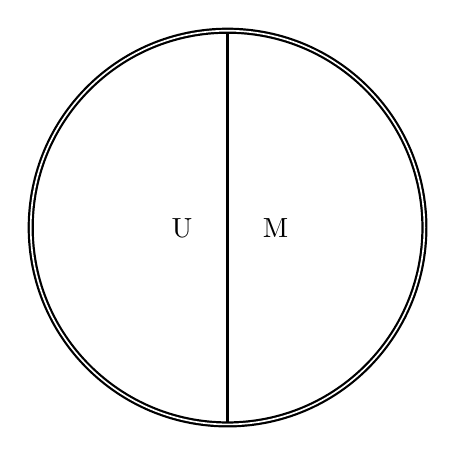
\begin{tikzpicture}[scale=.5]
			\draw[thick,double] (0,0) circle (5);
			%\draw[thick] (-5,0) -- (5,0);
			\draw[thick] (0,-4.95) -- (0,4.95);
				\node[label={[label distance=2mm]180:U}] at (0,0) {};
				\node[label={[label distance=2mm]360:M}] at (0,0) {};
		\end{tikzpicture}}
\end{figure}

\chapter{Contributions and conclusions}\label{ch:ConCon}

%\SelectTips{lu}{12}
\SelectTips{cm}{12}
%\SelectTips{eu}{12}

\section{Metathesis in linguistics}\label{sec:MetLin}
Previous works on metathesis have mainly viewed the phenomenon through a phonological lens.
This has led to much useful development of phonological
models and analyses which can account for metathesis.
In this work I have gone beyond a phonological account,
and have provided perhaps the first detailed study of both the form
\emph{and} function of metathesis in a single language, Amarasi.

Like some other languages with synchronic metathesis,
such as Rotuman, Leti, and Helong (see \srf{sec:MorMet}),
metathesis in Amarasi is not a unitary phenomenon.
Instead, we can identify three kinds of metathesis:
one kind of phonologically conditioned metathesis and two
kinds of morphological metathesis, one with a syntactic
function and one with a discourse function.

In the greater Timor region (and more widely) metathesis is
often used as a construct form marking attributive modification.
Other languages in which metathesis is a construct form
include Rotuman, Leti, Roma, Mambae, and Helong  (\srf{sec:MorMet}).
The large number of languages which have the same function for metathesis
is probably connected with the development of consonant-vowel metathesis.

Metathesis with a discourse function has been
reported for Luang, in which metathesis of verbs
occurs at certain points in the narrative structure, namely:
``Known information and mainline event information,
especially at peak points of the story.'' \citep[24]{tata15}.
However, under the analysis of \cite{tata15}, metathesis
in Luang is a phonological process which occurs
to join words into a single rhythm unit;
a phrase with only one stressed syllable.

Metathesis in Kwara'ae, in which both forms
are used in different speech registers,
could be construed as a kind of discourse metathesis.
Again, however, metathesis in Kwara'ae can be successfully analysed
as a result of the stress rules of the language \citep{he04}.

\largerpage
Neither syntactic nor discourse metathesis
in Amarasi can be reduced to being the accidental side affect of some other
phonological process (see \srf{sec:AltAppPhoMet}).
Instead, the two generalisations which allow
us to account for all the different phonological processes
found in the formation of M\=/forms
are an obligatory CVCVC foot (with empty C-slots)
and a rule of consonant-vowel metathesis; CV {\ra} VC /\'V{\gap}.

\cite{blga98} showed how a process of synchronic metathesis
can develop through a number of phonetically natural steps (see \srf{sec:OriMorMet})
and in \srf{sec:OriMetAma} I showed that there is evidence
that Amarasi developed its metathesis according to the pathway labelled \emph{compensatory metathesis} by \cite{blga98};
this is a kind of metathesis which originally arose in certain prosodically conditioned environments.

Metathesis in Amarasi is no longer restricted these environments.
Unlike Lunag or Kwara'ae, metathesis in Amarasi has
escaped from any original phonological constraints
and now runs throughout the whole language.
From the occurrence of isolated words
where nouns are cited in the U\=/form and verbs in the M\=/form,
right up to complex clause chaining phenomena such as tail-head linkage,
the single phenomenon the analyst encounters time and time again is metathesis.

Nearly all areas of Amarasi grammar interact with metathesis.
In Chapter \ref{ch:StrMetAma} I posited that the creation of a morphological metathesis paradigm
was part of the motivation for the imposition of the CVCVC foot to all words of the language
in order to provide the necessary machinery for consonant-vowel metathesis to operate,
and thereby allow each word to fill both cells of the morphological paradigm.
In this way metathesis has taken over the phonotactics of Amarasi
and become the central organising principle by which words are structured.

Phonotactics is not the only linguistic sub-domain to have been invaded by metathesis.
In Chapter \ref{ch:PhoMet} I showed that metathesis
interacts with prosodic structures by marking a clear
phonological boundary between two prosodic words.

In Chapter \ref{ch:SynMet} I showed that
it is metathesis which marks the structure of the noun and verb phrase
by marking the presence of an attributive modifier
which belongs to the same word class as the head of a phrase.

In Chapter \ref{ch:DisMet} I showed that in narratives
it is metathesis which advances the plot through tail-head linkage
and dependent coordination.
In multi-speaker discourse,
metathesis is the social glue which binds the conversation together.
Unmetathesised and metathesised forms are employed as question-answer pairs,
and signal the end of a conversational turn,
thereby carrying forward interactions between speakers.

Metathesis in Amarasi is not merely
an epiphenomenon or exotic curiosity.
Rather, it is a central feature around which other linguistic structures are organised.
In addition to being the key which unlocks the structure and genius
of the language, Amarasi metathesis is also the linguistic instantiation of two pervasive
ethnographic traits of the Amarasi people: identity and parallelism.
\section{Metathesis and identity}\label{sec:MetIde}

\begin{figure}[h]
	\caption{Self-identified varieties of Meto}\label{fig:SelIdeVarUabMeto-2}
	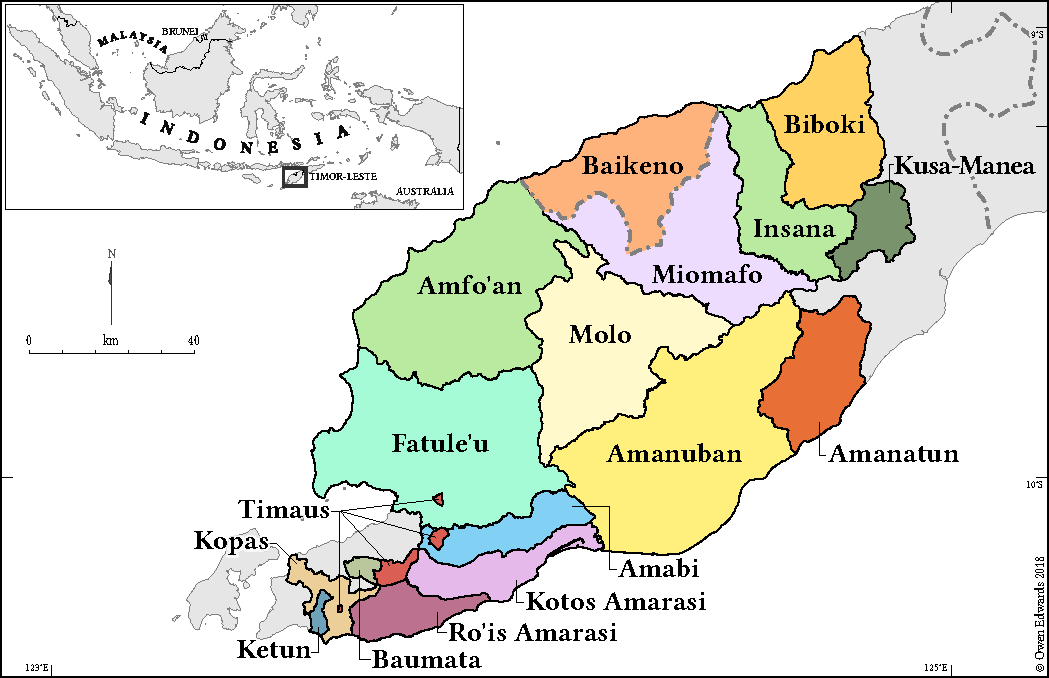
\includegraphics[width=\columnwidth]{Metos-LinLib.pdf}
\end{figure}

It is well known that language is frequently employed
as a marker of identity \citep{mi82,ed09,figa10}.
This is also the case in western Timor in which the four
main ethnic identities are delineated according to language:
Rote, Helong, Tetun, and the Atoni, who speak Meto.\footnote{
		Meto speakers refer to themselves in full as \ve{atoin paah metoʔ}
		or \ve{atoni paah metoʔ} `people of the dry land' (\citealt[i]{cu62}; \citealt[1]{scno71}).
		The term Atoni is from \ve{atoniʔ} in Amarasi
		or \ve{atoni} in other Meto varieties and means `man, person'.}

Within each of these groups, further identities also exist.
While the Atoni (Meto speakers) self-identify as
a single cultural and linguistic group,
they also acknowledge internal cultural and linguistic differences between groups.
The labels used for the prescriptively defined different groups,
as given in \frf{fig:SelIdeVarUabMeto-2},
correspond almost exactly to the historic kingdoms of the region.

One kind of cultural difference found between groups is different weaving traditions.
An example of Amarasi cloth, Amfo{\Q}an cloth, and Fatule{\Q}u cloth
is given in \frf{fig:ThrTypMetClo} below.
Further differences in weaving are also found between individual hamlets.
Thus, the use of blue lines between the geometric maroon patterns
in \frf{fig:AmaClo} is distinctive of Koro{\Q}oto hamlet
while the hamlet of Ponain, for instance, mainly uses yellow lines.

\begin{figure}[h]
  \begin{subfigure}[b]{0.32\textwidth}
		\frame{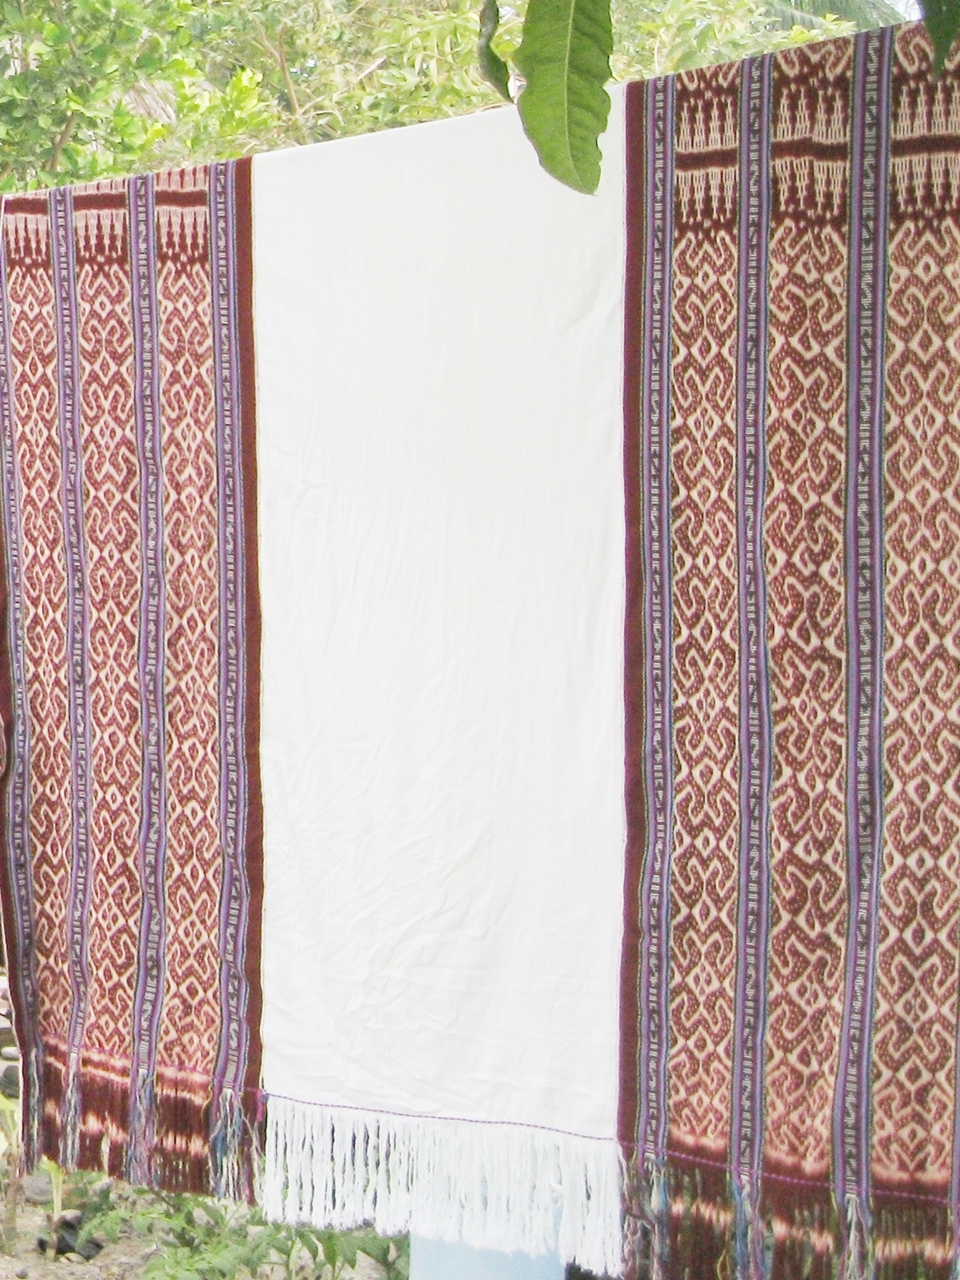
\includegraphics[width=\linewidth]{AmarasiCloth.jpg}}
		\caption{Amarasi cloth}\label{fig:AmaClo}
  \end{subfigure}
  \begin{subfigure}[b]{0.32\textwidth}
		\frame{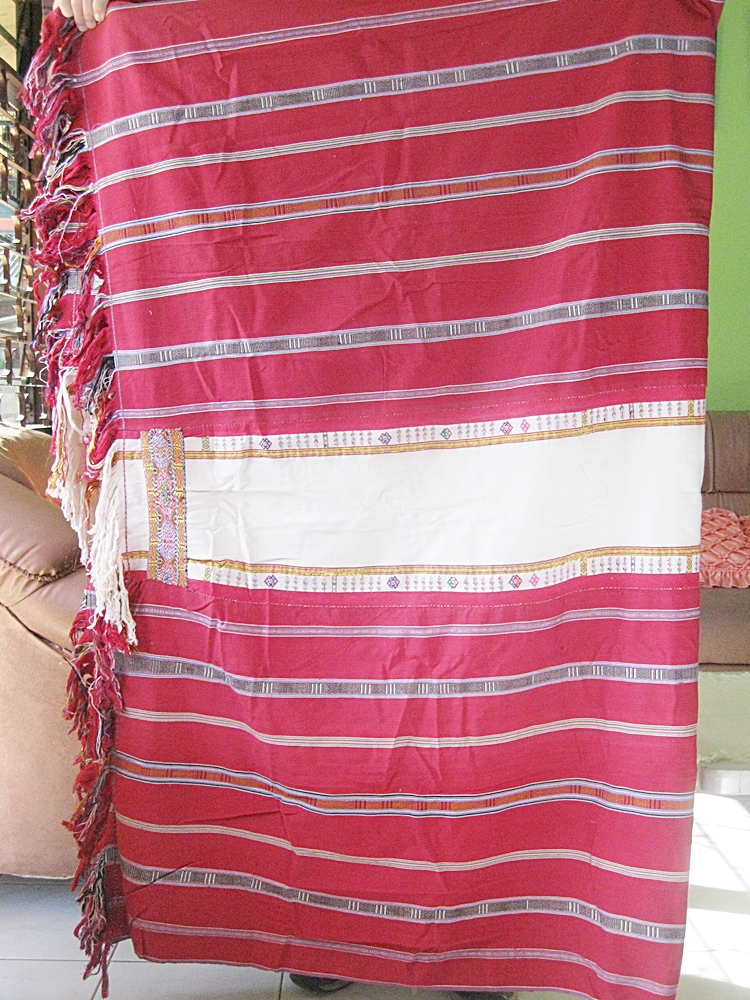
\includegraphics[width=\linewidth]{AmfoanCloth.jpg}}
		\caption{Amfo{\Q}an cloth}\label{fig:AmfClot}
  \end{subfigure}
  \begin{subfigure}[b]{0.32\textwidth}
		\frame{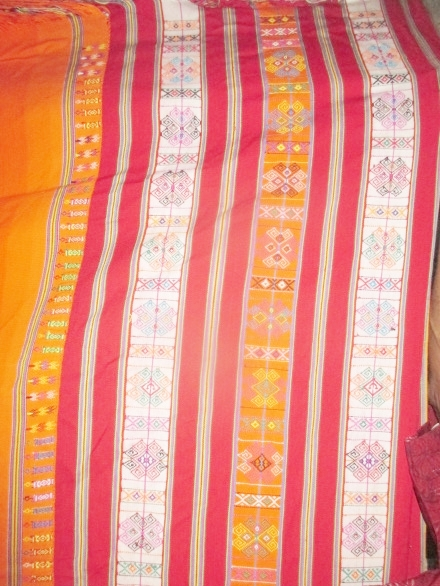
\includegraphics[width=\linewidth]{FatulequCloth.jpg}}
		\caption{Fatule{\Q}u cloth}\label{fig:FatClot}
  \end{subfigure}
	\caption{Three types of Meto cloth}\label{fig:ThrTypMetClo}
\end{figure}

Another example of enacted identity can be found in the 
different methods employed to count corn,
the traditional crop of western Timor.
As reported by \cite{grba11}, Kotos Amarasi counts
corn in units of \ve{rean}, with one \ve{rean} being 400 cobs of corn.
In the Tais Nonof variety of Amarasi,
corn is counted by the \ve{nifu} (thousand).
In some other regions corn is counted by \it{kuda} (Indonesian for `horse')
with one \it{kuda} consisting of 80 cobs of corn.

Such differences are salient to the Atoni.
When collecting data on Fatule{\Q}u I was accompanied
by my main Amarasi consultant, Heronimus Bani (Roni).
After I had collected a wordlist,
Roni asked about cloth design in Fatule{\Q}u;
what the different parts of the pattern were called,
and what these patterns symbolised, in fact
figure \frf{fig:FatClot} was taken by Roni.
He also asked how corn was counted in Fatule{\Q}u
and volunteered that in Amarasi corn was counted by \ve{rean}.

The Atoni agree that they speak a single language: Meto.
However, they also acknowledge that there are differences in how people speak
in different places, differences which can often accumulate to such an
extent that they seriously hinder communication.

In my experience, Atoni from different regions
often talk in a mixture of Meto and Indonesian/Kupang Malay.
Using Meto enables expression of their shared identity and
the use of Indonesian/Kupang Malay enables effective communication.
One or more speakers will also usually adapt their speech to
perceived norms of their interlocutors.

The Atoni are aware to varying degrees of salient differences between different varieties of Meto.
It is fairly common knowledge, for instance, that Amarasi has /r/ while
other varieties have /l/.\footnote{
		The situation is, in fact, more complex.
		Amabi and Kusa-Manea also have /r/ instead of /l/.
		Timaus has both /l/ and /r/
		(the latter of which has developed from *\j).
		These additional complexities do not enter into the
		popular discourse about differences.}
Similarly, on a more local scale speakers of Kotos Amarasi and Ro{\Q}is Amarasi
are aware of some differences between one another's speech,
and when asked, my Kotos consultants would gleefully try to imitate Ro{\Q}is speech.

One obvious kind of linguistic difference between
different varieties of Meto is lexical.
A selection of lexemes in several varieties of Meto
and other languages of western Timor is given in \trf{tab:LexDifUabMetVar}.
Although the difference between Meto other languages
is greater than that between individual varieties of Meto,
the internal diversity of Meto is not insignificant.

\begin{table}[h]
	\caption{Lexical differences between languages of western Timor}\label{tab:LexDifUabMetVar}
	\centering
	\begin{threeparttable}
	\stl{0.3em}\begin{tabular}{rllllll} \lsptoprule
									& `earth'					& `thorn'				& `mouse'			& `red'\su{†}		&	`big'					& `dream' 			\\ \midrule
			Amarasi			&	\ve{afu}				& \ve{aikaʔ}		& \ve{knafo}	& \ve{meʔe}			&	\ve{koʔu}			& \ve{na-mnei}	\\
			Amanuban		&	\ve{nain}				& \ve{sakunat}	& \ve{nafo}		& \ve{meeʔ}			&	\ve{ʔnaek}		& \ve{na-naeʔ}	\\
			Amanatun		&	\ve{nain}				& \ve{kasunat}	& \ve{nafo}		& \ve{meeʔ}			&	\ve{ʔnaek}		& \ve{na-naeʔ}	\\
			Fatule{\Q}u	&	\ve{afu}				& \ve{}					& \ve{ifo}		& \ve{mtasaʔ}		&	\ve{ʔnaek}		& \ve{n-unmaeʔ}	\\
			Molo				&	\ve{na\j an}		& \ve{katilaʔ}	& \ve{ifo}		& \ve{mtasaʔ}		&	\ve{ʔnaek}		& \ve{n-ʔunmaeʔ}\\
			Amfo{\Q}an	&	\ve{nai\j an}		& \ve{kalilaʔ}	& \ve{ifog}		& \ve{mtasaʔ}		&	\ve{ʔnaek}		& \ve{na-smaan}	\\
			Baikeno			&	\ve{nai\j aan}	& \ve{kalilaʔ}	& \ve{bifo}		& \ve{meeʔ}			&	\ve{ʔnaek}		& \ve{na-mnei}	\\
			Timaus			&	\ve{afi\j}			& \ve{katilaʔ}	& \ve{ifugw}	& \ve{meeʔ}			&	\ve{ʔnaek}		& \ve{n-mai}		\\
			Kopas				&	\ve{afu}				& \ve{katilaʔ}	& \ve{ifo}		& \ve{meeʔ}			&	\ve{ʔnaek}		& \ve{na-mnai}	\\
			Kusa-Manea	&	\ve{nian}				& \ve{tanaʔ}		& \ve{nafo}		& \ve{nuti}			&	\ve{binaiʔ}		& \ve{na-mnei}	\\ \hline
			Helong			&	\it{dale}				& \it{duliʔ}		& \it{blaho}	& \it{mea}			&	\it{tene}			& \it{natloa}		\\
			Lole (Rote)	&	\it{dae}				& \it{dilak}		& \it{lafo}		& \it{mbilas}		&	\it{inahuu-k}	& \it{meʔi}			\\
			Dela (Rote)	&	\it{rae}				& \it{maŋgouʔ}	& \it{lafo}		& \it{mbilas}		&	\it{ine-ʔ}		& \it{na-lamein}\\
			Tetun				&	\it{rai}				& \it{ktarak}		& \it{laho}		& \it{mean}			&	\it{boo}			& \it{meʔi}			\\ \lspbottomrule
		\end{tabular}
			\begin{tablenotes}
				\item[†] In Amarasi \ve{mtasaʔ} means `ripe' and \ve{meʔe mtasaʔ} `maroon'.
			%%	\item[‡]
			%%	\item[§]
			%%	\item[‖] 
			%%	\item[¶] 
			\end{tablenotes}
	\end{threeparttable}
\end{table}

\subsection{Realisation of U\=/forms and M\=/forms}
Another marker of linguistic identity among the Atoni is metathesis: different ways of realising
U\=/forms and M\=/forms, different environments in which these forms are used
and different functions of these forms.
Some differences in the realisation of U\=/forms and M\=/forms
between eight different varieties of Meto
are given in \trf{tab:VarUfoMfo},
with identical forms indicated by identical colours.

\begin{table}[h]
	\caption[Variation in U\=/forms and M\=/forms]
					{Variation in U\=/forms and M\=/forms\su{†}}\label{tab:VarUfoMfo}
	\centering\stl{0.2em}
		\begin{threeparttable}
			\begin{tabular}{rllllllllll}\lsptoprule
	&	\mc{2}{l}{`three'} 					&	\mc{2}{l}{`dog'} 					&	\mc{2}{l}{`wood, tree'} 					&	\mc{2}{l}{`fire'} 					&	\mc{2}{l}{`day'} 					\\	\midrule
	&	\tsc{u}		&	\tsc{m}		&	\tsc{u}		&	\tsc{m}		&	\tsc{u}		&	\tsc{m}		&	\tsc{u}		&	\tsc{m}		&	\tsc{u}		&	{\Mvv}		\\	
Kotos\sub{\tsc{k}}	&	\it{tenu}	{\cellcolor{blue!40}}	&	\it{teun}	{\cellcolor{blue!40}}	&	\it{asu}	{\cellcolor{blue!40}}	&	\it{aus}	{\cellcolor{blue!40}}	&	\it{hau}	{\cellcolor{blue!40}}	&	\it{hau}	{\cellcolor{blue!40}}	&	\it{ai}	{\cellcolor{blue!40}}	&	\it{ai}	{\cellcolor{blue!40}}	&	\it{neno}	{\cellcolor{blue!40}}	&	\it{neeŋgw=}	{\cellcolor{blue!40}}	\\	
Kotos\sub{\tsc{f}}	&	\it{tenu}	{\cellcolor{blue!40}}	&	\it{teun}	{\cellcolor{blue!40}}	&	\it{asu}	{\cellcolor{blue!40}}	&	\it{aus}	{\cellcolor{blue!40}}	&	\it{hau}	{\cellcolor{blue!40}}	&	\it{hau}	{\cellcolor{blue!40}}	&	\it{ai}	{\cellcolor{blue!40}}	&	\it{ai}	{\cellcolor{blue!40}}	&	\it{neno}	{\cellcolor{blue!40}}	&	\it{neoŋg=}	{\cellcolor{green!50}}	\\	
Ro{\Q}is\sub{\tsc{s}}	&	\it{tenu}	{\cellcolor{blue!40}}	&	\it{teun}	{\cellcolor{blue!40}}	&	\it{asu}	{\cellcolor{blue!40}}	&	\it{aus}	{\cellcolor{blue!40}}	&	\it{hau}	{\cellcolor{blue!40}}	&	\it{hau}	{\cellcolor{blue!40}}	&	\it{ai}	{\cellcolor{blue!40}}	&	\it{ai}	{\cellcolor{blue!40}}	&	\it{neno}	{\cellcolor{blue!40}}	&	\it{neenb=}	{\cellcolor{yellow!75}}	\\	
Amanub.	&	\it{tenu}	{\cellcolor{blue!40}}	&	\it{teun}	{\cellcolor{blue!40}}	&	\it{asu}	{\cellcolor{blue!40}}	&	\it{aus}	{\cellcolor{blue!40}}	&	\it{hau}	{\cellcolor{blue!40}}	&	\it{hau}	{\cellcolor{blue!40}}	&	\it{ai}	{\cellcolor{blue!40}}	&	\it{ai}	{\cellcolor{blue!40}}	&	\it{neno}	{\cellcolor{blue!40}}	&	\it{neen=}	{\cellcolor{orange!85}}	\\	
%Ketun	&	\it{tenu}	{\cellcolor{blue!40}}	&	\it{teun}	{\cellcolor{blue!40}}	&	\it{asaw}	{\cellcolor{green!50}}	&	\it{aus}	{\cellcolor{blue!40}}	&	\it{hau}	{\cellcolor{blue!40}}	&	\it{hau}	{\cellcolor{blue!40}}	&	\it{ai}	{\cellcolor{blue!40}}	&	\it{ai}	{\cellcolor{blue!40}}	&	\it{nenao̯}	{\cellcolor{green!50}}	&			\\	
Kualiin	&	\it{tenu}	{\cellcolor{blue!40}}	&	\it{teun}	{\cellcolor{blue!40}}	&	\it{asaw}	{\cellcolor{green!50}}	&	\it{aus}	{\cellcolor{blue!40}}	&	\it{hau}	{\cellcolor{blue!40}}	&	\it{hau}	{\cellcolor{blue!40}}	&	\it{ai}	{\cellcolor{blue!40}}	&	\it{ai}	{\cellcolor{blue!40}}	&	\it{nenao̯}	{\cellcolor{green!50}}	&	\it{neen=}	{\cellcolor{orange!85}}	\\	
Baikeno	&	\it{tenu}	{\cellcolor{blue!40}}	&	\it{teen}	{\cellcolor{green!50}}	&	\it{asu}	{\cellcolor{blue!40}}	&	\it{aos}	{\cellcolor{green!50}}	&	\it{haub}	{\cellcolor{green!50}}	&	\it{hau}	{\cellcolor{blue!40}}	&	\it{ai\j}	{\cellcolor{green!50}}	&	\it{ai}	{\cellcolor{blue!40}}	&	\it{neno}	{\cellcolor{blue!40}}	&	\it{neemb=}	{\cellcolor{red!70}}	\\	
Amfo{\Q}an	&	\it{tenu}	{\cellcolor{blue!40}}	&	\it{teen}	{\cellcolor{green!50}}	&	\it{asug}	{\cellcolor{yellow!75}}	&	\it{asu}	{\cellcolor{yellow!75}}	&	\it{haug}	{\cellcolor{yellow!75}}	&	\it{hau}	{\cellcolor{blue!40}}	&	\it{ai\j}	{\cellcolor{green!50}}	&	\it{ai}	{\cellcolor{blue!40}}	&	\it{nenog}	{\cellcolor{yellow!75}}	&	\it{neeŋgw=}	{\cellcolor{blue!40}}	\\	
Timaus	&	\it{tenu}	{\cellcolor{blue!40}}	&	\it{teenw}	{\cellcolor{yellow!75}}	&	\it{asi\j}	{\cellcolor{orange!85}}	&	\it{asu}	{\cellcolor{yellow!75}}	&	\it{haa\j}	{\cellcolor{orange!85}}	&	\it{hau}	{\cellcolor{blue!40}}	&	\it{aar}	{\cellcolor{yellow!75}}	&	\it{ai}	{\cellcolor{blue!40}}	&	\it{nenugw}	{\cellcolor{orange!85}}	&	\it{neeŋgw=}	{\cellcolor{blue!40}}	\\	
Fatule{\Q}u	&	\it{tenu}	{\cellcolor{blue!40}}	&	\it{teenw}	{\cellcolor{yellow!75}}	&	\it{asu}	{\cellcolor{blue!40}}	&	\it{aus}	{\cellcolor{blue!40}}	&	\it{haub}	{\cellcolor{green!50}}	&	\it{hau}	{\cellcolor{blue!40}}	&	\it{aa\j}	{\cellcolor{orange!85}}	&	\it{ai}	{\cellcolor{blue!40}}	&	\it{neno}	{\cellcolor{blue!40}}	&	\it{neenb=}	{\cellcolor{yellow!75}}	\\	
Kopas\sub{\tsc{t}}	&	\it{tenu}	{\cellcolor{blue!40}}	&	\it{teun}	{\cellcolor{blue!40}}	&	\it{asu}	{\cellcolor{blue!40}}	&	\it{aus}	{\cellcolor{blue!40}}	&	\it{haag}	{\cellcolor{red!70}}	&	\it{hau}	{\cellcolor{blue!40}}	&	\it{aa\j}	{\cellcolor{orange!85}}	&	\it{ai}	{\cellcolor{blue!40}}	&	\it{neno}	{\cellcolor{blue!40}}	&	\it{neon=}	{\cellcolor{purple!75}}	\\	
Kopas\sub{\tsc{u}}	&	\it{tenu}	{\cellcolor{blue!40}}	&	\it{teenw}	{\cellcolor{yellow!75}}	&	\it{asu}	{\cellcolor{blue!40}}	&	\it{aus}	{\cellcolor{blue!40}}	&	\it{haagw}	{\cellcolor{purple!75}}	&	\it{hau}	{\cellcolor{blue!40}}	&	\it{aa\j}	{\cellcolor{orange!85}}	&	\it{ai}	{\cellcolor{blue!40}}	&	\it{neno}	{\cellcolor{blue!40}}	&			\\	
			\lspbottomrule
			\end{tabular}
				\begin{tablenotes}
					\item [\su{†}]	Kotos\sub{\tsc{k}} = Kotos Amarasi from Koro{\Q}oto hamlet,
													Kotos\sub{\tsc{f}} = Kotos Amarasi from Fo{\Q}asa{\Q} hamlet,
													Ro{\Q}is\sub{\tsc{s}} = Ro{\Q}is Amarasi from Suit hamlet,
												%	Amarasi\sub{\tsc{f}} = Kotos Amarasi from Fo{\Q}asa{\Q} hamlet,
													Amanub. = Amanuban from Niki-niki,
												%	Baikeno = 
													Kualiin = Amanuban from Kualin village,
													Amfo{\Q}an = Naitbelak Amfo{\Q}an from Ta{\Q}en hamlet,
													Fatule{\Q}u = Bineon-Koa{\Q} hamlet,
													Kopas\sub{\tsc{t}} = Tuale{\Q}u hamlet,
													Kopas\sub{\tsc{u}} = Usapisonba{\Q}i hamlet,
				\end{tablenotes}
		\end{threeparttable}
\end{table}

\trf{tab:VarUfoMfo} shows that there is an extensive array
of realisations for U\=/forms and M\=/forms.
The four different processes which occur are: metathesis,
consonant insertion, diphthongisation, and vowel shift or assimilation.
Different combinations of these processes not only occur in different Meto varieties,
but two particular varieties of Meto do not necessarily treat all words
of the same phonotactic shape in the same way.

Nouns undergo metathesis in all (known) varieties before vowel-initial enclitics,
but with or without insertion of different consonants
(which occurs with or without assimilation of final /n/).
A number of varieties mark U\=/forms ending in a vowel sequence
by consonant insertion, though in different varieties different consonants are inserted
and are accompanied by different degrees of vowel assimilation.
Words which end in CV{\#} can have basic M\=/forms
marked by metathesis (with presence or lack of various kinds of vowel assimilation)
or by lack of consonant insertion, with some Meto varieties
also showing variation between different word classes.

In the context of other linguistic alternations and markers of identity,
such differences in the realisation of U\=/forms and M\=/forms
are an additional strategy for marking linguistic identity.
They are also perceived this way by both insiders and outsiders.

In her analysis of consonant insertion in Nai{\Q}bais Amfo{\Q}an,
\cite{cu18} reports that this process is seen by
speakers as a marker of identity.
Thus, \citeauthor{cu18}'s main consultant told her when she began her work:
{``Here in Amfo{\Q}an we add consonants at the end of sentences.
That's how you know someone is from Amfo{\Q}an.''}
Similarly, this process is viewed by outsiders as distinctive.
When I collected Amfo{\Q}an data I was accompanied
by speakers of Amanuban from So{\Q}e.
On the way up to Amfo{\Q}an, my friends reported
that ``all the words there end in <g>'',
referring to the process of consonant insertion used to form the U\=/forms
of nouns which end in /o/ and /u/ (\srf{sec:EmpCSloConIns}).

Similarly, Amarasi speakers from Koro{\Q}oto
hamlet know that speakers from the hamlet of Fo{\Q}asa{\Q} have different M\=/forms before enclitics
(e.g. as seen in Koro{\Q}oto \ve{nee{\ng}gw=ee}, Fo{\Q}asa{\Q} \ve{neo{\ng}g=ee} `the sky, day').
Likewise, when collecting data on Fatule{\Q}u, Kopas, and Timaus while accompanied
by Roni (my main Amarasi consultant), the different patterns
of metathesis and consonant insertion in these
Meto varieties were very salient to him.

Furthermore, differences in the realisation of U\=/forms and M\=/forms
are quite difficult for speakers of different varieties of Meto to copy.
In discussions with Roni after collecting Timaus data, he was generally unable to reproduce
the kinds of consonant insertion seen there, despite the correspondences
between Amarasi and Timaus being regular.

Similarly, I have overheard speakers of Amanuban
attempt, but fail, to correctly copy patterns of metathesis in Amarasi.
While Amanuban speakers know there are differences in
vocabulary and metathesis between their speech and Amarasi,
they are not necessarily able to combine the two together correctly.
This is in contrast with other some other differences,
such as the use of /r/ in Amarasi where Amanuban has /l/.

\largerpage
Examples \qf{ex:AmanubanMet} and \qf{ex:AmarasiMet} below
show the same way of saying a number of phrases in Amanuban and Amarasi.
In both varieties verbs before the inceptive enclitic \ve{=een} undergo consonant insertion,
metathesis, and vowel assimilation, but with different consonants inserted.
Where Amarasi inserts /ɡw/, Amanuban inserts /w/
and where Amarasi inserts /\j/, Amanuban inserts a palatal glide /j/.

\begin{multicols}{2}
	\begin{exe}
		\ex{Amanuban:}\label{ex:AmanubanMet}
			\begin{xlist}
				\ex{\glll	hai m-faan\tbr{j}=een.\\
									hai m-fani=ena\\
									{\hai} \m-back{\Mv}={\een}\\
						\glt	`We'll head back now.'}
				\ex{\glll	hai m-naa\tbr{w}=een.\\
									hai m-nao=ena\\
									{\hai} \m-go{\Mv}={\een}\\
						\glt	`We'll get going now.'}
				\ex{\glll	hai m-\tbr{fiinj}=een.\\
									hai m-fini=ena\\
									{\hai} \m-pass{\Mv}={\een}\\
						\glt	`We'll keep going now.'}
			\end{xlist}
		\ex{Amarasi:}\label{ex:AmarasiMet}
			\begin{xlist}
				\ex{\glll	hai m-faan\tbr{\j}=een.\\
									hai m-fani=ena\\
									{\hai} \m-back{\Mv}={\een}\\
						\glt	`We'll head back now.'}
				\ex{\glll	hai m-naa\tbr{gw}=een.\\
									hai m-nao=ena\\
									{\hai} \m-go{\Mv}={\een}\\
						\glt	`We'll get going now.'}
				\ex{\glll	hai m-\tbr{koo\ng gw}=een.\\
									hai m-kono=ena\\
									{\hai} \m-pass{\Mv}={\een}\\
						\glt	`We'll keep going now.'}
			\end{xlist}
	\end{exe}
\end{multicols}

In addition to the differences in consonant insertion,
there are also differences in vocabulary:
Amarasi has \ve{{\rt}kono} `pass' and Amanuban has \ve{{\rt}fini} `pass'.
While Amanuban speakers are aware of such differences,
they are not necessarily able to combine the two together.
The top line of example \qf{ex:AmarasiError} below was said
by one of my Amanuban friends when trying to adapt
their speech to Amarasi.

\begin{exe}\let\eachwordtwo=\itshape\let\eachwordthree=\itshape
	\ex{\glll	\textnormal{\tcb{incorrect Amarasi:}} 			hai m-koom\j=een.		\,\,\textnormal{\tcb{{\la} hai m-komi=een}} \\
						\textnormal{\tcb{\hp{in}correct Amarasi:}}	hai m-koo{\ng}gw=een.	\,\,\textnormal{\tcb{{\la} hai m-kono=een}} \\
						\textnormal{\tcb{\hp{in}correct Amanuban:}}	hai m-fiinj=een.			\,\,\textnormal{\tcb{{\la} hai m-fini=een}}\\
				\glt		\lh{incorrect Amanuban:} `We'll keep going now.' \txrf{observation}}\label{ex:AmarasiError}
\end{exe}

In this example, the Amanuban speaker has had some success
in selecting the correct verb, though has selected the wrong medial nasal with /m/ instead of /n/.\footnote{
		The selection of the incorrect nasal /m/ rather than correct
		/n/ probably came about partly in order to differentiate
		this form from \ve{{\rt}koni} `copulate'.}
They have also correctly identified a rule along the lines of
``Amarasi inserts /\j/ where we insert /j/''.
Because of this they have inserted /\j/ for this sentence.
However, the difference in the quality of the final vowels of
Amarasi \ve{{\rt}kono} `pass' and Amanuban \ve{{\rt}fini} `pass'
means that application of this rule yields an incorrect result in this instance.

\subsection{Environments for U\=/forms and M\=/forms}
The realisation of the U\=/form and M\=/form of words
is one dimension across which speakers of Meto can mark identity.
Another dimension is the environments in which metathesis occurs.
For instance, in Kotos Amarasi metathesis is blocked before words
which begin with a consonant cluster (\srf{sec:CCIniMod}),
while in Ro{\Q}is Amarasi metathesis freely occurs
before such words (\srf{sec:RoqAnaCCIniMod}).
This yields pairs such as Kotos \ve{u\tbr{mi} kbubuʔ} and Ro{\Q}is \ve{u\tbr{im} kbubuʔ} `round house',
or Kotos \ve{kru\tbr{ru} tnana-f} Ro{\Q}is \ve{kru\tbr{ur} tnana-f} `middle finger'.
More examples are given in \trf{tab:RoqMetConClu} on \prf{tab:RoqMetConClu}.

Similarly, consonant-final verbs do not undergo
metathesis in Kotos Amarasi (\srf{sec:ConFinVer}),
while in Ro{\Q}is Amarasi verbs with a final /n/ are eligible
to undergo metathesis (\srf{sec:MforFinConClu}).
Two examples of Ro{\Q}is phrases with metathesis
resulting in a final consonant cluster are given in \qf{ex:08/10/14, p.113 ch:ConCon}
and \qf{ex:09/10/14, p.114 ch:ConCon} below along with their Kotos equivalents.

\begin{multicols}{2}
	\begin{exe}\let\eachwordtwo=\itshape
		\ex{\glll	\textnormal{\tcb{Ro{\Q}is:}} siin na-sa\tbr{ap}=\tbr{n}.\\
							\textnormal{\tcb{Kotos:}} siin na-sa\tbr{pa}=\tbr{n}.\\
							{} {\siin} {\na}-kick={\einV}\\
				\glt	\lh{Kotos: }`They're playing soccer.'}\label{ex:08/10/14, p.113 ch:ConCon}
							%\txrf{observation 08/10/14, p.113}}\label{ex:08/10/14, p.113 ch:ConCon}
		\ex{\glll	\textnormal{\tcb{Ro{\Q}is:}} raump=ein n-ma\tbr{et}=\tbr{n}.\\
							\textnormal{\tcb{Kotos:}} paku=n n-ma\tbr{te}=\tbr{n}.\\
							{} light={\ein} {\n}-die={\einV}\\
				\glt	\lh{Kotos: }`The lights have died.'}\label{ex:09/10/14, p.114 ch:ConCon}
							%\txrf{observation 09/10/14, p.114}}\label{ex:09/10/14, p.114 ch:ConCon}
	\end{exe}
\end{multicols}

Another dimension across which differences in metathesis
can be marked is in the functions of U\=/forms and M\=/forms.
In this book I have described and analysed the functions of U\=/forms and M\=/forms
only in Kotos Amarasi (as spoken in Koro{\Q}oto hamlet).
Although the full details remain to be investigated,
data from other varieties of Meto shows that metathesis
behaves differently in different varieties.

Thus, for instance, in Amfo{\Q}an \citep{cu18}
and Timaus (own fieldnotes) verbs take the U\=/form
much more often than they do in Kotos Amarasi.
This is clearly exemplified in \qf{ex:Mark 1:2}--\qf{ex:Mark 16:7}
below with a selection of parallel passages from the gospel
of Mark in Amarasi and Amfo{\Q}an \citep{UBB18}.
The Amfo{\Q}an version is given below the Amarasi.
Verbs which are metathesised in Amarasi but
unmetathesised in Amfo{\Q}an are indicated.

\begin{exe}\let\eachwordtwo=\itshape
	\ex{\glll	na-hu\tbr{un} na-ʔko naiʔ Yesus n-a\tbr{it}  iin mepu,\\
						na-hu\tbr{nu} na-ʔko nai  Yesus n-a\tbr{iti} iin mepug,\\
						\na-first \na-{\qko} {\naiq} Jesus \n-pick.up {\iin} work\\
			\glt	`Before Jesus began his work,' \txrf{Mark 1:2a}}\label{ex:Mark 1:2}
	\ex{\glll	n-ok ranan mee henatiʔ paah naan \hp{na-}bisa {\a}n-ha\tbr{ek} na-ba\tbr{ar}?\\
						na-tuin lalan mee henatiʔ paah naan na-beʔi a|n-ha\tbr{ke} na-ba\tbr{la}?\\
						3-with way what {\he} country {\naan} 3-able \a\n-stand \na-constant\\
			\glt	`In what way will that country be able to endure?'\txrf{Mark 3:24}}\label{ex:Mark 3:24}
	%\ex{\glll	a|n-bi oors =ees, siin n-e\tbr{ik} siin aanh =ein nema=n n-eu naiʔ Yesus\\
						%a|n-bi tabug meseʔ, sini n-e\tbr{ki} siin anah =siin nema=n n-oi nai  Yesus\\
						%\n-{\ek} time one {\siin} \n-bring {\siin} child ={\ein} come={\einV} \n-{\eu} {\naiq} Jesus\\
			%\glt	`One time, they brought their children to Jesus'\txrf{Mark 10:13}}\label{ex:Mark 10:13}
	\ex{\glll	ma oras maans =ii {\a}n-ma\tbr{eb} on nana =te\\
						ma tabug manas {} a|n-ma\tbr{be} on nane\\
						and time sun ={\ii} \a\n-afternoon like {\naan} ={\te}\\
			\glt	`And when the sun was about to go down,'\txrf{Mark 11:19}}\label{ex:Mark 11:19}
	\ex{\glll	onaim hii {\a}m-fa\tbr{in} nai rab{\tl}raab! \\
						{ees on naan} hii a|m-fa\tbr{ni} nai lab{\tl}laab!\\
						and.so {\hii} \a\m-return already {\prd}quick\\
			\glt	`So return quickly!'\txrf{Mark 16:7}}\label{ex:Mark 16:7}
%	\ex{\glll	\\
%						\\
%						\\
%			\glt	`'\txrf{}}\label{ex:}
\end{exe}

The Amfo{\Q}an gospel of Mark has been translated
by native speakers from the Amarasi version.
This means that the differences in metathesis seen
in \qf{ex:Mark 1:2}--\qf{ex:Mark 16:7} above
reflect deliberate decisions by Amfo{\Q}an speakers
to unmetathesise certain verbs to yield a more natural translation.

While the exact function of metathesis in Amfo{\Q}an
discourse remains to be fully worked out,
it is clear that the analysis I proposed for Amarasi
in Chapter \ref{ch:DisMet} cannot be straightforwardly
extended to cover the Amfo{\Q}an data.

Regarding metathesis in the syntax, my Timaus
data shows that certain noun phrases occur
with a metathesised head while others do not.
In my Timaus data I have ten names of different
kinds of birds composed of the noun \ve{kolo} `bird'
(phrase-final \ve{kolugw}) followed by a nominal modifier.
Of these, the head is metathesised in six,
unmetathesised in four, and one shows variation.
These Timaus bird names are given in \trf{tab:BirNamTim} on the next page.
Whatever the basis for this variation in Timaus,
it is clearly different from Amarasi, in which head
nouns obligatorily occur metathesised when
followed by an attributive modifier.

\begin{table}[ht]
	\centering\caption{Bird names in Timaus}\label{tab:BirNamTim}
	\begin{tabular}{rll}\lsptoprule
		Head			&	Modifier			&	gloss	\\	\midrule
		\ve{kolo}	&	\ve{anal}			&	`sparrow'	\\	
		\ve{kolo}	&	\ve{fumaki\j}	&	`orange-banded thrush'	\\	
		\ve{kolo}	&	\ve{kael}			&	`yellow-crested cockatoo'	\\	
		\ve{kolo}	&	\ve{kefar}		&	`pigeon'	\\	
		\ve{kolo}	&	\ve{kuis}			&	`thrush'	\\	
		\ve{kolo}	&	\ve{luan}			&	`wild pigeon'	\\	
		\ve{kolo}	&	\ve{kaaʔ}			&	`crow'	\\	\hline
		\ve{kool}	&	\ve{kaaʔ}			&	`crow'	\\	
		\ve{kool}	&	\ve{kitaʔ}		&	`great-billed parrot'	\\	
		\ve{kool}	&	\ve{kuki\j}		&	`collared dove'	\\	
		\ve{kool}	&	\ve{otos}			&	`barred dove'	\\	
		\lspbottomrule
	\end{tabular}
\end{table}

Similarly, in Insana data given by \cite{scno71},
certain noun phrases have an unmetathesised head
while others have a metathesised head.
Examples of phrases with a metathesised head include
\ve{lais metoʔ} `traditional matters' (Amarasi \ve{rais metoʔ}),
and \ve{neon tees} `sunset' (Amarasi \ve{neon tees}).
Examples of phrases with an unmetathesised head include \ve{mone feʔu} `son-in-law,
\emph{lit.} new male' (Amarasi \ve{moen feʔu}) and
\ve{tasi mone} `southern sea, \emph{lit.} male sea' (Amarasi \ve{tais mone}).
Again, this reflects a different use of metathesis in the syntax
between Insana and Amarasi.

Metathesis is a marker of identity within the Atoni ethno-linguistic group.
The presence of metathesis in this language cluster
sets it apart from other local groups, such as Tetun and the Rote languages
-- though not from Helong (\srf{sec:Hel}) --
and the differences between the forms, functions, and environments
of metathesis between different varieties of Meto
vary and serve to mark sub-identities among the Atoni.
\section{Metathesis and unmetathesis as complementary pairs}\label{sec:MetPar}
In addition to marking differences in identity,
metathesis -- the pairing of two forms which together make a fully grammatical functional whole --
also reflects the fundamental Atoni
conceptualisation of societal and cosmic organisation.
The complementarity of metathesis and unmetathesis in the syntax,
and the parallelism of unmetathesis with metathesis in the discourse
reflects the Atoni division of the world into complementary pairs.

The relationship between M\=/forms and U\=/forms in the syntax (Chapter \ref{ch:SynMet})
is represented in \frf{fig:SynMet},
in which each is one half of a whole with the latter completing the former.
Similarly, the relationship between U\=/forms and M\=/forms in the discourse (Chapter \ref{ch:DisMet})
is visualised in \frf{fig:DisMet},
with the latter resolving the former.

\begin{figure}[ht]
  \begin{subfigure}[b]{0.49\textwidth}
		\centering{\Huge
			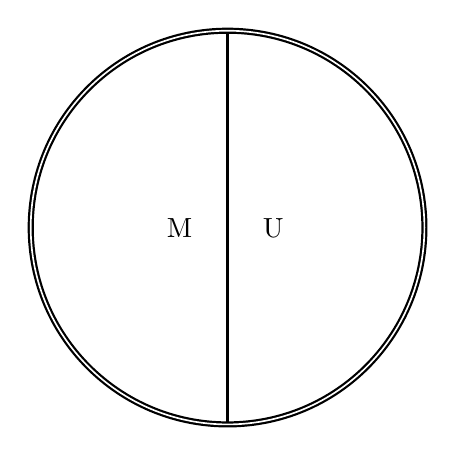
\begin{tikzpicture}[scale=.5]
				\draw[thick,double] (0,0) circle (5);
				\draw[thick] (0,-4.95) -- (0,4.95);
					\node[label={[label distance=2mm]180:M}] at (0,0) {};
					\node[label={[label distance=2mm]360:U}] at (0,0) {};
			\end{tikzpicture}}
		\caption{Syntactic metathesis}\label{fig:SynMet}
  \end{subfigure}
  \begin{subfigure}[b]{0.49\textwidth}
		\centering{\Huge
			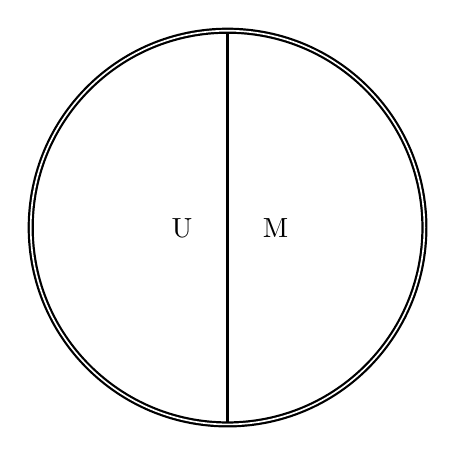
\begin{tikzpicture}[scale=.5]
				\draw[thick,double] (0,0) circle (5);
				\draw[thick] (0,-4.95) -- (0,4.95);
					\node[label={[label distance=2mm]180:U}] at (0,0) {};
					\node[label={[label distance=2mm]360:M}] at (0,0) {};
			\end{tikzpicture}}
		\caption{Discourse metathesis}\label{fig:DisMet}
  \end{subfigure}
	\caption{Complementary metatheses}\label{fig:CompMet}
\end{figure}

An example of each of these complementary pairs
is given below with \qf{ex:120923-2, 1.39 ch:ConCon}
showing a syntactically conditioned M\=/form‖U\=/form pair and example
\qf{ex:130909-6, 0.36 ch:ConCon} showing a discourse-driven U\=/form‖M\=/form pair.

\begin{exe}
	\ex{\glll	na-tuuʔ \bxA{ta\tbr{in}} \bxB{tu\tbr{ni,}} tua, =ma {\lk}\\
						na-tuʔu {\gp}tani {\gp}tuni tua  =ma\\
						\na-make.knot {\gp}rope{\tbrM} {\gp}gewang.palm{\tbrU} {\tua} =and\\
			\glt	`(He) ties up a rope made from gewang palm (leaves)'
						\txrf{120923-2, 1.39} {\emb{120923-2-01-39.mp3}{\spk{}}{\apl}}}\vspace{4pt}\label{ex:120923-2, 1.39 ch:ConCon}
	\ex{\glll	m-ak hai nua =kai \bxA{m-taiko\tbr{bi}} =m hai \bxB{m-ma\tbr{et}} okeʔ {\lk}\\
						m-ak hai nua =kai {\gp}m-taikobi =ma hai {\gp}m-mate okeʔ \\
						\m-say {\hai} two {\kai} \gp\m-fall{\tbrU} =and {\hai} \gp\m-die{\tbrM} all \\
			\glt	`So we two will fall down and (then) both die.'
						\txrf{130909-6, 0.39} {\emb{130909-6-00-39.mp3}{\spk{}}{\apl}}}\label{ex:130909-6, 0.36 ch:ConCon}
\end{exe}

The parallelism and complementarity of U\=/forms with M\=/forms
and M\=/forms with U\=/forms reflects fundamental Atoni philosophical
and conceptual notions of the structure of the world
as being composed of binary and complementary pairs.
One explicit use of these pairs in linguistic structure is in Amarasi poetry.

\subsection{Metathetic poetic parallelism}\label{sec:MetPoePar}
The role of parallelism in Timor has already been touched on
in \srf{sec:PoePar}, in which I discussed the structure of poetry.
Poetry in Amarasi makes use of canonical parallelism \citep{fo88,fo14},
the pairing of pre-determined and semantically related words.
Amarasi poetry is an explicit use of the complementarity
which exists between metathesis and unmetathesis.

Example \qf{ex:140726 0.00--0.05} below,
drawn from a performed chant (\ve{aʔa sramat}) ,
shows the way in which semantic parallelism operates in Amarasi.
Nearly every content word co-occurs in the same line in a structurally
parallel way with a semantically similar content word,
giving three sets of doublets in a single line.
Doublets are joined by linking lines.

\begin{exe}
	\ex{Amarasi chant (\ve{aʔa sramat}): \txrf{140726}{\emb{140726-00-00-00-05.mp3}{\spk{}}{\apl}}}\vspace{5pt}\label{ex:140726 0.00--0.05}
	\begin{xlist}
		\ex{\gll	\bxA{baisenu-t} =ma \bxB{ronaen} n-eu \rnode{C}{\psframebox[linewidth=0.4pt]{mutiʔ}} =ma \rnode{D}{\psframebox[linewidth=0.4pt]{mnatuʔ}} et
							{\lks} {\ncbar[arm=5pt,angle=90,linewidth=0.4pt]{-}{C}{D}}\\
							{\gp}look.up =and {\gp}greeting \n-{\eu} {\gp}silver =and {\gp}gold {\et} \\ \vspace{5pt}}
		\sn{\gll	\bxA{muit} ma-hine-ʔ =ma \bxB{mnatuʔ} neee {\lks}\\
							{\gp}silver {\ma}-know-{\ma} =and {\gp}gold \tsc{pause}\\
				\glt	`Greetings and honour to all people, who are like silver and gold, wise and knowledgeable silver and gold,' \txrf{0.00}}
		\ex{\gll	MA-HINE-Ɂ \\
							{\ma}-know-{\ma} \\
				\glt	`So wise.'	\txrf{0.05}}
	\end{xlist}
\end{exe}

When the doublet consists of a pair of verbs,
it is possible, though not obligatory,
for the first verb to occur in the U\=/form and the second in the M\=/form.
Two examples are given in \qf{ex:130825-3, 1.21 ch:ConCon} and \qf{ex:MsimoMaMtoup} below.
In both examples the indicated doublets are both semantically and morphologically parallel.
Thus, for instance, in example \qf{ex:130825-3, 1.21 ch:ConCon}
the semantic doublet, \ve{m-tenu \tcb{‖} mu-haof} `umbrella ‖ shade'
is also a morphological doublet composed of U\=/form‖M\=/form.

\begin{exe}
	\ex{\glll	henatiʔ \bxA{m-te\tbr{nu}} =m \bxB{mu-ha\tbr{of}} too tafaʔ =kai {\lks}\\
						henatiʔ {\gp}m-tenu =ma {\gp}mu-hafo too tafaʔ =kai\\
						{\he} \gp\m-umbrella{\tbrU} =and \gp\muu-shade{\tbrM} citizen small {\kai}\\
			\glt	`So that you might shade [doublet] us small people.'
						\txrf{130825-3, 1.21} {\emb{130825-3-01-21.mp3}{\spk{}}{\apl}}}\label{ex:130825-3, 1.21 ch:ConCon}
		\ex{\glll	hai m-nonaʔ =ma m-fee fuaʔturuʔ reʔ hai \\
							hai m-nonaʔ =ma m-fee fuaʔturuʔ reʔ hai \\
							{\hai} {\m}-hand{\Uc} =and {\m}-give offering {\req} {\hai} \\ \vspace{5pt}}\label{ex:MsimoMaMtoup}
		\sn{\glll	\bxA{n-si\tbr{mo}} =ma \bxB{n-to\tbr{up}} =siin mi-ʔko hoo ʔnima-m \hspace{5mm} a-ma-neka-b, {\lks}\\
							{\gp}n-simo =ma {\gp}n-topu =sini mi-ʔko hoo ʔnima-m {} a-ma-neka-b,\\
							\gp\n-receive{\tbrU} =and \gp\n-receive{\tbrM} ={\siin} {\mi}-{\qko} {\hoo} hand-{\mg} {} {\at}-{\ma}-love-{\b}\\
				\glt	`We give offerings we received from your loving hand.' \txrf{observation}}
\end{exe}

Another kind of metathetic parallelism occurs in chants of the \ve{aʔa sramat} genre.
In such chants a leader of a group will chant one line,
after which the rest of the group repeats a word from that line.
It is common, though not obligatory, for the repeated word 
to occur in the opposite U\=/form/M\=/form compared with the form the leader used.
If the leader uses a U\=/form, the group typically uses an M\=/form, and vice versa.\footnote{
	Thanks go to Charles Grimes for bringing this to my attention.}

One example is given in \qf{ex:120715-0, 0.30-0.35} below,
in which a verbal U\=/form said by the leader
is repeated in the M\=/form by the rest of the group.
Such examples are formally identical to the use of metathesis
in question-answer pairs (\srf{sec:QuePar}).
In each instance one speaker uses a verbal U\=/form which is completed
by the next speaker(s) using an M\=/form of the same verb.

\begin{exe}
	\ex{\begin{xlist}
		\ex{\glll	ka= t-tok{\tl}took =ma tak{\tl}t-ak =fa =te, hiit ta-ʔeuk =ma \bxA{\ve{ta-te\tbr{fa}}} =m neee\\
							ka= t-tok{\tl}toko =ma tak{\tl}t-ak =fa =te hiti ta-ʔeku =ma {\gp}ta-tefa =ma neee\\
							{\ka}= \t-{\prd}sit{\M} =and \prd\t-say ={\fa} ={\te} {\hiit} {\ta}-meet{\M} =and {\gp}{\ta}-meet{\tbrU} =and {\nehh}\\
				\glt	`We don't just sit and talk, we interact and meet.' \txrf{120715-0, 0.30} {\emb{120715-0-00-30-00-35.mp3}{\spk{}}{\apl}}}\
		\ex{\glll \bxA{\ve{TA-TE\tbr{EF}}} \\
							{\gp}ta-tefa \\
							{\gp}{\ta}-meet{\tbrM} \\
				\glt	{\gp}`We meet.' \txrf{0.35}}
	\end{xlist}}\label{ex:120715-0, 0.30-0.35}
\end{exe}

It is also possible for the repeated word to be a noun.
When this occurs, the first instance of the
noun often occurs with a vowel-initial enclitic attached
which triggers the M\=/form (Chapter \ref{ch:PhoMet}).
The whole group will then repeat the noun
without the enclitic; thus in the U\=/form.
Two examples are given in \qf{ex:140726 1} and \qf{ex:140726 2} below,
each of which comes from a single prayer.

In example \qf{ex:kniunq} the noun phrase \ve{Smana Kninuʔ} `Holy Spirit'
is modified by the determiner \ve{=aa}, and thus occurs in the M\=/form.
The final word of this noun phrase is then chanted by the whole group, though in the U\=/form.

\begin{exe}
	\ex{Prayer composed in poetic language: \txrf{140726, 0.21} {\emb{140726-00-21.mp3}{\spk{}}{\apl}}}\label{ex:140726 1}
	\begin{xlist}
		\ex{\glll	iin kuu-n ees reʔ a|n-sia =ma n-naib =kii n-eik ina Smana \bxA{\ve{Kni\tbr{unʔ}=aa}} =m neee\\
							ini kuu-n esa reʔ {\a}n-sia =ma n-nabi =kii n-eki ina smana-f {\gp}kninuʔ=aa =ma neee\\
							{\iin} self-{\N} {\esc} {\req} {\a\n}-lead =ma {\n}-guide{\M} ={\kii} \n-use{\M} {\iin} spirit{\Mc} {\gp}holy{\tbrMv}={\aa} =and {\nehh}\\
				\glt	`It is he who leads and guides us with his Holy Spirit'}\label{ex:kniunq}
		\ex{\gll	RO \bxB{\ve{KNI\tbr{NUɁ}}}\\
							very {\gp}holy{\tbrU}\\
				\glt	`He is very holy.'}\label{ex:kninuq}
	\end{xlist}
\end{exe}

Similarly, in example \qf{ex:areokt} the noun \ve{arekot} `good'
is followed by a vowel-initial enclitic and occurs in the M\=/form.
This word is then repeated by the whole group in \qf{ex:arekot} in the U\=/form.

\begin{exe}
	\ex{Prayer composed in poetic language: \txrf{140726, 0.27} {\emb{140726-00-27.mp3}{\spk{}}{\apl}}}\label{ex:140726 2}
	\begin{xlist}
		\ex{\glll	etun hii ar=kii m-muiʔ reon =ma runat \hspace{20mm} \bxA{\ve{a-re\tbr{ok}-\tbr{t}=aa}} =m neee\\
							etun hii ar=kii m-muʔi reon =ma runat {} {\gp}a-reko-t=aa =ma neee\\
							so.that {\hii} all={\kii} \m-have{\M} event =and plan {} \hspace{1.2mm}\at-good{\tbrMv}-{\at}={\aa} =and {\nehh}\\
				\glt	`So that you will have success in your event and plan.'}\label{ex:areokt}
		\ex{\gll	\bxB{\ve{A-RE\tbr{KO}-\tbr{T}}}\\
							{\gp}{\at}-good{\tbrU}-{\at}\\
				\glt	{\gp}`It is very good.'}\label{ex:arekot}
	\end{xlist}
\end{exe}

The pattern in examples \qf{ex:140726 1} and \qf{ex:140726 2}
with paired nominals is U\=/form‖M\=/form, while with verbs
the pattern is M\=/form‖U\=/form, as seen in \qf{ex:120715-0, 0.30-0.35}.
The reason noun doublets occur in the order M\=/form‖U\=/form,
and verb doublets occur in the order U\=/form‖M\=/form
is straightforwardly explained by their order in non-poetic speech.
In the syntax, an M\=/form noun signals an incomplete attributive
phrase which requires completion from a following form, typically a U\=/form (Chapter \ref{ch:SynMet}).
In the discourse, a U\=/form occurs first, and requires resolution
from a subsequent clause, which typically contains an M\=/form (Chapter \ref{ch:DisMet}).

The use of alternate M\=/forms and U\=/forms in Amarasi poetry
-- a style of speech in which parallel forms are obligatory --
is an explicit utilisation of the complementarity which
exists between metathesis and unmetathesis.

\subsection{Cultural and conceptual complementarity}
As discussed in \srf{sec:MetLin}, metathesis is a key
element of the Amarasi language around which many other linguistic structures are organised.
However, more than simply being a key linguistic structure,
the complementarity found between metathesis and unmetathesis
is paralleled by the Atoni conceptualisation of the world
as being composed of complementary parts.

At the beginning of his discussion of the
``Political system as approached in Timorese [Atoni] thinking'',
\citet[408]{scno71} gives a set of complementary concepts,
some of which are given in \trf{tab:AtoParCon}.
Of these concepts he states:
``All these pairs of opposites fit into one scheme and combine to form one important dichotomy.
%All of the concepts in the left-hand column are related by a scheme of mental associations,
%while the same is true of those in the right hand column.
[\ldots] The one is inconceivable without the other.''

\begin{table}[h]
	\caption[Atoni complementary concepts]{Atoni complementary concepts \citep[408]{scno71}}\label{tab:AtoParCon}
	\centering
		\begin{tabular}{rcl} \lsptoprule
			female 		&--& male\\
			wife			&--& husband\\
			sister 		&--& brother\\
			female ancestor	&--&male ancestor\\
			inside		&--&outside\\
			west/north&--&east/south\\
			yellow		&--&red\\
		\lspbottomrule
		\end{tabular}
\end{table}

The Atoni conceptualisation of social and cosmic order
is classified and arranged around such complementary pairs.
A visual analogy of this complementarity can be seen on any piece of Atoni cloth,
illustrated in \frf{fig:AmaSca} below with an Amarasi scarf.
Each half of this cloth, along both horizontal and vertical axes,
is opposite to and a mirror image of the other half;
each half is the complement of the other, and neither is complete without the other.

\begin{figure}[h]\setlength\fboxsep{-0.5pt}\setlength\fboxrule{0.75pt}
	\caption{Amarasi scarf}\label{fig:AmaSca}
	\fbox{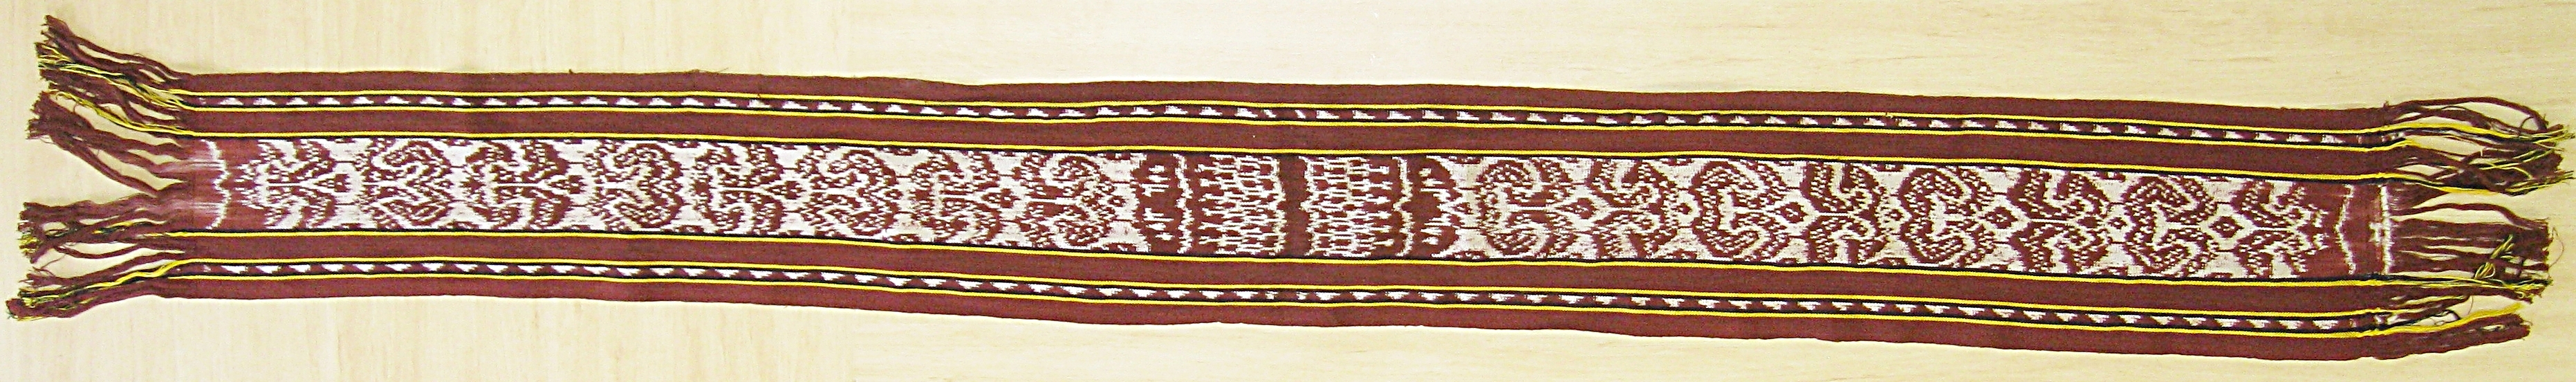
\includegraphics[width=\columnwidth]{AmarasiScarf2.jpg}}
\end{figure}

Dualism and complementarity in the Atoni world
goes beyond the simple ``two-column analysis'' represented in \trf{tab:AtoParCon}.
There are complex relationships between these categories which
include asymmetry, analogical cross-over and recursive parallelism \citep{fo89}.

Of all complementary pairs, one significant relationship
is that of \ve{feto-mone} `female-male'.
A category classified as \ve{feto} `female'
will have a complementary category classified as \ve{mone} `male'.
The classification of pairs as \ve{feto-mone} `female- male'
is not necessarily linked to the actual biological gender
of the members of the pairs,
but is rather a way of expressing and describing
the complementarity which exists between the two categories.

One instance in which the \ve{feto-mone} relationship holds
is in two families related by marriage.
When two families are related by marriage, those who have given their daughter
in marriage (the wife-givers) are classified as \ve{mone} `male'
in relation to those who have received the woman.
Those who have received the woman are classified
as \ve{feto} `female' in relation to the wife givers.

%	Dear Owen
%	No need for confusion. Wife-Giver is Mone; Wife-Taker is Feto.
% As recipient of another’s lineage’s women, that lineage is feto to its wife-giver (mone).
%	Look at my paper (attached) which spells things out explicitly and clearly.
%	Will try to come to your seminar: where will it be? 
%	Will Mark be there?  It would be good to talk to him.
%	Yours, Jim

In addition to being complementary, with each completing the other,
the relationship between the wife-givers and
the wife-receivers is also asymmetrical.
\cite{scno71} analysed this asymmetry in terms of
``superordination'' and ``subordination'':

\begin{quote}
%In the kinship system the \ve{feto-mone} [feminine-masculine] relationship
%is found to exist between two \ve{ume} [houses] which are allied by affinal relationships.
%The \ve{ume} [house] with which the natal \ve{ume} [house] has affinal
%relationships via its daughters is called \ve{feto} [feminine]
%and the one with which it has such relationships via its sons is \ve{mone} [masculine].
[\ldots] the [female] \ve{ume} [house] receiving a woman (who is the source of life)
is inferior in respect of the [male] one which is the giver of life and hence its superior.
This relationship of subordination and superordination is expressed in terms of \ve{feto-mone}.
But at the same time the term \ve{feto-mone} indicates that the one cannot exist without the other,
as life is impossible without the unity of male and female.
Thus \ve{feto-mone} groups form each other's complements. \hfill\citep[411]{scno71}
\end{quote}

While \citeauthor{scno71} accurately identifies the asymmetrical
nature of this relationship the language of ``superordination'' and ``subordination''
may not be the best description of the asymmetry.
Instead, as the givers of the gift, the wife-givers
are in a relationship of precedence to the \ve{feto} `female' wife-receivers \citep{fo94,fo99}.
Because the wife-receivers are \ve{feto} `female' and the wife-givers are \ve{mone} `male',
in this particular context \ve{mone} `male' precedes \ve{feto} `female'.
This is an example of categorical asymmetry \citep[47]{fo94}.

The relationship between \ve{feto} `female' and \ve{mone} `male' groups is not fixed.
As discussed by \cite{fo99}, these relationships are fluid and can be reversed.
Groups constantly seek to re-negotiate their relationship,
with wife-receivers seeking to return a woman to their wife-givers,
and thus reversing their relationship.

A similar conclusion is also reached by \cite{mcw02}
in his study of place and precedence in Amanuban.
While the domain of Amanuban was politically organised with
dual classification, ``these structures tended to
be flexible, strategic, and opportunistic'' \cite[287]{mcw02}.
Complementary categories are tools, not restrictions,
for Atoni thought and classification.

Another area in which the \ve{feto-mone} `female-male'
complementary pair occurs is in the traditional political structure of Atoni society.
In Insana, for instance, the supreme ruler at the centre of a realm
was classified as \ve{feto} `female'.
This \ve{feto} ruler was the guardian of the sacred objects
and responsible for the proper maintenance of ritual.
He was complemented by another ruler, classified as \ve{mone} `male'.
This \ve{mone} ruler was the executive authority of the realm
and had responsibility for warfare \citep[371ff]{scno71}.\footnote{
		Both rulers were biologically male.}

In this context, it would be erroneous to identify
the \ve{mone} `male' ruler as preceding the \ve{feto} `female' ruler.
Instead, it is the supreme \ve{feto} `female' ruler at the centre of the domain,
around whom all the other parts revolve and who holds all these parts together,
who precedes the \ve{mone} `male' ruler.

What is most important in this relationship is the complementarity between
the \ve{feto} `female' ruler and the \ve{mone} `male' ruler,
with both co-existing in balancing roles.
The complementarity between \ve{feto-mone} `female-male',
in which each is one half of a whole,
is represented in \frf{fig:FemMasRel} below.

\begin{figure}
  \begin{subfigure}[b]{0.49\textwidth}
			\centering{\LARGE
				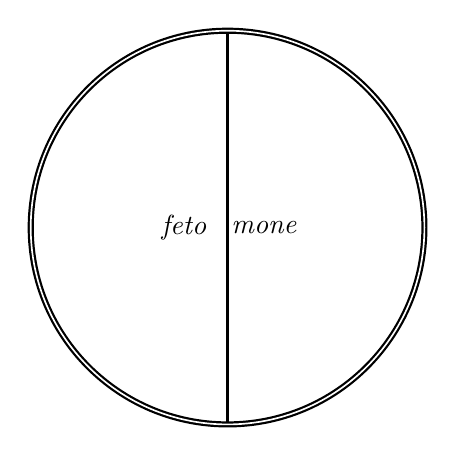
\begin{tikzpicture}[scale=.5]
					\draw[thick,double] (0,0) circle (5);
					\draw[thick] (0,-4.95) -- (0,4.95);
						\node[label={[label distance=-0mm]180:\ve{feto}}] at (0,0) {};
						\node[label={[label distance=-2mm]360:\ve{mone}}] at (0,0) {};
				\end{tikzpicture}}
		\caption{Female-male pair}\label{fig:FemMasRel}
  \end{subfigure}
  \begin{subfigure}[b]{0.49\textwidth}
			\centering{\LARGE
				\begin{tikzpicture}[scale=.5]
					\draw[thick,double] (0,0) circle (5);
					\draw[thick] (0,-4.95) -- (0,4.95);
						\node[label={[label distance=-2mm]180:\ve{moneʔ}}] at (0,0) {};
						\node[label={[label distance=-2mm]360:\ve{nanan\vp{ʔ}}}] at (0,0) {};
				\end{tikzpicture}}
		\caption{Outside-inside pair}\label{fig:OutIns}
  \end{subfigure}
	\caption{Complementary pairs}\label{fig:CompPai}
\end{figure}

Another pair of complementary cncepts in in Atoni culture
is \ve{moneʔ-nanan} `outside-inside', or `periphery-centre'.
The \ve{nanan} `inside, centre' is symbolic of unity between different parts.
It is the location of the supreme ruler in a realm,
and the area of a house to which agnates
(blood relatives) have full access \citep{cu64}.

Just as the \ve{feto-mone} `female-male' pair is asymmetrical,
the \ve{moneʔ-nanan} `outside-inside' pair is also asymmetrical,
with \ve{nanan} `inside' in precedence to
\ve{moneʔ} `outside' \citep{cu64,scno71,fo89}.
The relationship between the pair \ve{moneʔ-nanan}
is represented in \frf{fig:OutIns}.

The phonological similarity of the terms \ve{mone} `male'
and \ve{moneʔ} `outside' has given rise to a link in Atoni thought
between these two terms and has lead to what \cite{fo89} terms analogical cross-over:
``Male [\ve{mone}], which is superior in certain contexts
is associated with the outside [\ve{moneʔ}], which is inferior'' \cite[49]{fo89}.
The association between \ve{mone} `male' and \ve{moneʔ} `outside',
has also lead to an association between the complements of each of these terms,
with \ve{feto} `female' being associated with \ve{nanan} `inside'.\footnote{
		The term \ve{mone} `male' is a reflex of Proto-Malayo-Polynesian *maRuqanay `male'.
		The term \ve{moneʔ} `outside' is probably
		inherited from Proto-Malayo-Polynesian *ma-udehi `behind',
		also reflected by Amarasi \ve{na-muni} `be at the end' and \ve{munif} `young'.
		Whatever the ultimate etymology of the terms \ve{mone} `male' and \ve{moneʔ} `outside',
		it is the folk etymology ascribed to them by speakers
		which has created (or reinforced) the link between the two \citep[49]{fo89}.}

This association has lead to analogical crossover \citep{fo89}.
The member of each pair with precedence
is linked to the member of the other pair which does not have precedence.
This analogical cross-over is represented in \frf{fig:AnaCro} below
in which each member of each asymmetrical pair is connected
with the opposite member of the other asymmetrical pair.

\begin{figure}[h]
\caption{Analogical cross-over}\label{fig:AnaCro}
	\begin{minipage}{.49\textwidth}
			\centering{\LARGE
				\begin{tikzpicture}[scale=.5]
					\draw[thick,double] (0,0) circle (6);
					\draw[thick,double] (-5.95,0) -- (5.95,0);
					\draw[thick] (0,-5.95) -- (0,5.95);
						\node(a)[label={[label distance=-7mm]90:\ve{feto}}] at (-2.5,2.5) {};
						\node(b)[label={[label distance=-5mm]90:\ve{mone}}] at (2.5,2.5) {};
						\node(c)[label={[label distance=-8mm]90:\ve{moneʔ}}] at (-2.5,-2.5) {};
						\node(d)[label={[label distance=-8mm]90:\ve{nanan}}] at (2.5,-2.5) {};
						\draw[thick,<->] (a) -- (d);
						\draw[thick,<->] (c) -- (b);
				\end{tikzpicture}}
	\end{minipage}
	\begin{minipage}{.49\textwidth}
			\centering{\LARGE
				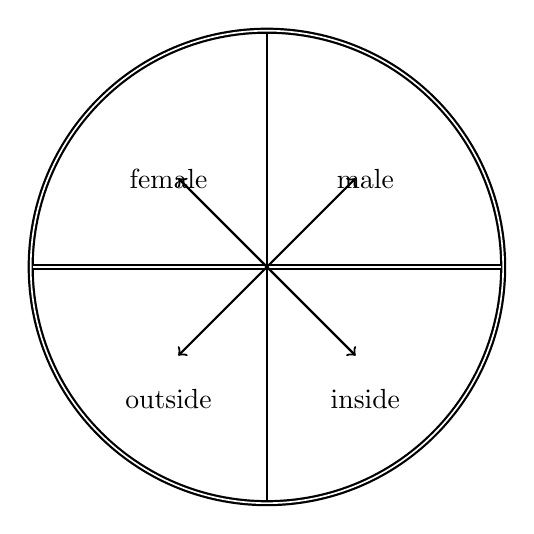
\begin{tikzpicture}[scale=.5]
					\draw[thick,double] (0,0) circle (6);
					\draw[thick,double] (-5.95,0) -- (5.95,0);
					\draw[thick] (0,-5.95) -- (0,5.95);
						\node(a)[label={[label distance=-5mm]90:{female}}] at (-2.5,2.5) {};
						\node(b)[label={[label distance=-5mm]90:{male}}] at (2.5,2.5) {};
						\node(c)[label={[label distance=-8mm]90:{outside}}] at (-2.5,-2.5) {};
						\node(d)[label={[label distance=-8mm]90:{inside}}] at (2.5,-2.5) {};
						\draw[thick,<->] (a) -- (d);
						\draw[thick,<->] (c) -- (b);
				\end{tikzpicture}}
	\end{minipage}
\end{figure}

One instance of this association has been seen in the fact that the \ve{feto} `female ruler
is located in the \ve{nanan} `centre' of the realm.
Another example of this association is seen in the categorisation
of the \ve{tasi} `sea, ocean', which is classified as consisting of two parts.
The \ve{nanan} `inner' circle of sea near the coast and bays
is the \ve{tais feto} `female sea', and the distant \ve{moneʔ} `outer' part
is known as the \ve{tais mone} `male sea' \citep[50]{cu64}.
This means that the northern Savu Sea is the \ve{tais feto} `female sea'
and the southern Timor Sea is the \ve{tais mone} `male sea',
as illustrated in \frf{fig:TimSea}

\begin{figure}[h]
	\caption{Timor and its seas}\label{fig:TimSea}
	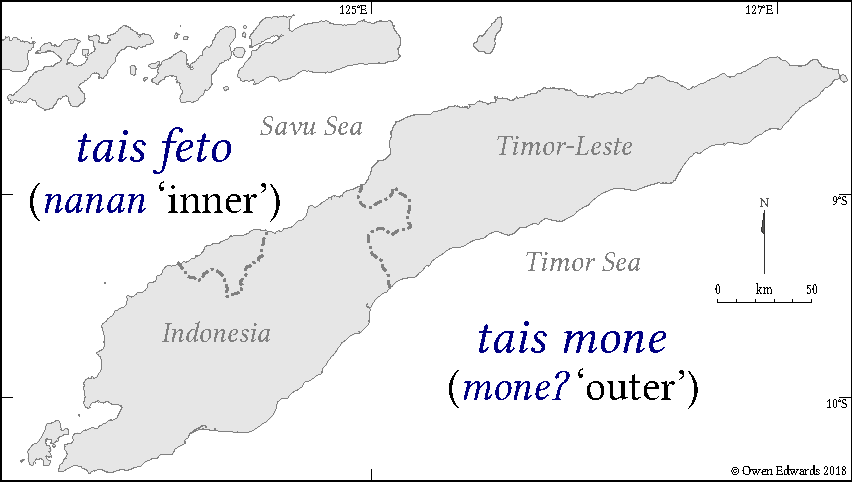
\includegraphics[width=0.8\columnwidth]{TimorSeas.pdf}
\end{figure}

\subsection{Metathetic parallel complementarity}\label{sec:MetParCom}
It is within this rich world of symbolic dualistic and complementary
classification that I place my analysis of metathesis in Amarasi.
Unmetathesised forms and metathesised forms are one another's complements.
This is demonstrably a fact of linguistic structure.
In the syntax, an M\=/form cannot occur in isolation and must be completed by a U\=/form.
In the discourse a U\=/form does not occur alone
and must be completed by another form, typically an M\=/form.

The identification of U\=/forms and M\=/forms as complementary pairs
is not equivalent to noting that these forms are formal opposites.
Instead, this identification is based on their usage,
the fact that each form must occur with the other in certain contexts.
Furthermore, in Amarasi poetry
-- a genre in which parallelism is obligatory --
unmetathesised and metathesised forms
are explicitly used as complementary pairs,
as discussed in \srf{sec:MetPoePar} above. %\footnote{
		%That U\=/forms and M\=/forms are complementary pairs
		%and not merely opposites can be illustrated with a negative example.
		%Within Amarasi phonology the phoneme /b/
		%and the phoneme /p/ are opposites:
		%/b/ is a voiced obstruent and /p/ is a voiceless obstruent.
		%However, there is no instance in which these two phonemes are deliberately paired together.
		%These two phonemes may be opposites, but they are not complements.}

Syntactic M\=/forms (M\sub{\tsc{s}}) are complemented by syntactic U\=/forms (U\sub{\tsc{S}}),
and discourse U\=/forms (U\sub{\tsc{d}}) are complemented by discourse M\=/forms (M\sub{\tsc{d}}).
In addition, the syntactic M\sub{\tsc{s}}‖U\sub{\tsc{s}} relationship
is itself paralleled and complemented by the opposite discourse U\sub{\tsc{d}}‖M\sub{\tsc{d}} relationship.
That M\=/forms require completion in the syntax is paralleled by the fact
that in the discourse U\=/forms which require completion.
The parallel relationship between the syntactic M\sub{\tsc{s}}‖U\sub{\tsc{s}} pair
and discourse U\sub{\tsc{d}}‖M\sub{\tsc{d}} pairs is represented in \frf{fig:AmaMet} below.
With an example of each given in \qf{ex:120923-2, 1.39 ch:ConCon2} and \qf{ex:130909-6, 0.36 ch:ConCon2}.

\begin{figure}[h]
	\caption{Metathesis and unmetathesis in Amarasi}\label{fig:AmaMet}
	\centering{\Huge
		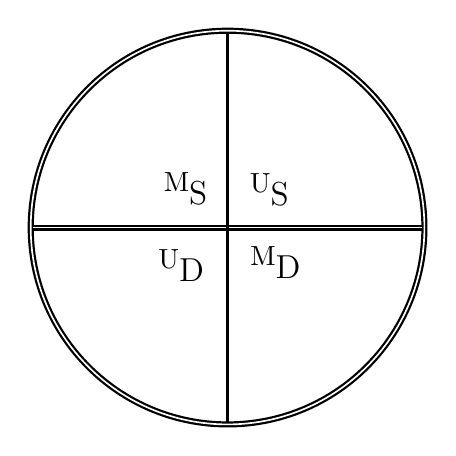
\begin{tikzpicture}[scale=.5]
			\draw[thick,double] (0,0) circle (5);
			\draw[thick,double] (-4.95,0) -- (4.95,0);
			\draw[thick] (0,-4.95) -- (0,4.95);
				\node[label={[label distance=.5mm]45:U\sub{\large S}}] at (0,0) {};
				\node[label={[label distance=.5mm]125:M\sub{\large S}}] at (0,0) {};
				\node[label={[label distance=.5mm]325:M\sub{\large D}}] at (0,0) {};
				\node[label={[label distance=.5mm]225:U\sub{\large D}}] at (0,0) {};
		\end{tikzpicture}}
\end{figure}

\begin{exe}
	\ex{Syntactic metathetic complementarity M\sub{\tsc{s}}‖U\sub{\tsc{s}}:}\vspace{4pt}\label{ex:120923-2, 1.39 ch:ConCon2}
	\sn{\glll	na-tuuʔ \bxA{ta\tbr{in}} \bxB{tu\tbr{ni,}} tua, =ma {\lk}\\
						na-tuʔu {\gp}tani {\gp}tuni tua  =ma\\
						\na-make.knot {\gp}rope{\tbrM\tbr{\sub{\tsc{s}}}} {\gp}gewang.palm{\tbrU\tbr{\sub{\tsc{s}}}} {\tua} =and\\
			\glt	`(He) ties up a rope made from gewang palm (leaves)'
						\txrf{120923-2, 1.39} {\emb{120923-2-01-39.mp3}{\spk{}}{\apl}}}\vspace{4pt}\label{120923-2, 1.39 ch:ConCon}
	\ex{Discourse metathetic complementarity U\sub{\tsc{d}}‖M\sub{\tsc{d}}:}\vspace{4pt}\label{ex:130909-6, 0.36 ch:ConCon2}
	\sn{\glll	m-ak hai nua =kai \bxA{m-taiko\tbr{bi}} =m hai \bxB{m-ma\tbr{et}} okeʔ {\lk}\\
						m-ak hai nua =kai {\gp}m-taikobi =ma hai {\gp}m-mate okeʔ \\
						\m-say {\hai} two {\kai} \gp\m-fall{\tbrU\tbr{\sub{\tsc{d}}}} =and {\hai} \gp\m-die{\tbrM\tbr{\sub{\tsc{d}}}} all \\
			\glt	`So we two will fall down and (then) both die.'
						\txrf{130909-6, 0.39} {\emb{130909-6-00-39.mp3}{\spk{}}{\apl}}}
\end{exe}

This is an example of analogical cross-over similar to
the association between \ve{feto-mone} `female-male'
and \ve{moneʔ-nanan} `outside-inside' discussed above.
In the case of metathesis, the association
is not between two formally similar (and perhaps related) forms
but instead it is between two formally identical forms,
with the same derivation which occur at different levels of the grammar.

The relationship between the four metathesis forms in \frf{fig:AmaMet} is
an instance of what I term \emph{cyclical complementarity}.
A syntactic M\=/form is complemented by a syntactic U\=/form,
which is paralleled by a discourse M\=/form which is the complement
of a discourse U\=/form, which is paralleled by a syntactic M\=/form,
and so on \emph{ad infinitum}.
Such cyclical complementarity is also found in
systems of marriage exchange in this region (whether formalised or informal),
whereby the wife-receivers will eventually return a woman to their wife-givers,
and thereby become the wife-givers, and so on.
Among the Atoni, for instance:

\begin{quote}
[\ldots] it is to the advantage of wife-givers to maintain their
asymmetric relation with their wife-takers and to the advantage of wife-takers
to reverse this relationship by returning a woman to their wife-givers [\ldots]
\citep{fo99}
%\hfill \cite[32]{fo99}
\end{quote}

The complementarity between metathesis and unmetathesis in Amarasi
and its strong congruence with the conceptual framework,
cosmic classification, and social organisation of Amarasi speakers
raises a number of interesting questions,
which I only pose up at this point.

Firstly, to what extent does the complementarity between unmetathesis and
metathesis occur in other Meto varieties?
Speakers of other Meto varieties have the same conceptual frameworks
as speakers of Amarasi. Thus, we expect this relationship to hold,
even if U\=/forms and M\=/forms have different forms and functions.
To answer this question will require a detailed study of
metatheses across other varieties of Meto.

Secondly, is the prevalence of synchronic metathesis in the greater Timor region
(see \frf{fig:CVMetTimReg} on page \pageref{fig:CVMetTimReg}) linked in any way
to the widespread use of complementary and dualistic classification in this region?
Answering this question will require a study of whether other regions
in which complementarity is common also have linguistic structures
which are complementary in a way that parallels that of metathesis in Amarasi.

Finally, how did the complementary nature of metathesis and unmetathesis arise in Amarasi?
Is it simply an accidental by-product of the environments
in which a phonological process became morphological?
Or is it a result of speakers (consciously or unconsciously)
noticing things about culture and mirroring them in grammar, and vice versa?
%If the latter, this could indicate that the any grammar-culture barrier
%is considerably more porous than some have thought.

One fruitful avenue of work which may help answer this last
question is a thorough structural examination of poetry and
verbal art in Meto. In poetry the complementarity of U\=/forms
and M\=/forms is explicitly utilised by speakers in more fluid
way than is seen in the syntax or discourse.
It may be the case that poetry was the domain of
language in which the complementarity between U\=/forms and M\=/forms first began.

For now, however, the last word and final statement on the
source and origin, as well as the reasons and grounds
of the parallelism and complementarity of metathesis and unmetathesis
in Amarasi should be given to the Amarasi speakers themselves,
expressed in their own poetic language composed in parallel pairs:

\begin{exe}
	\ex{Chant (\ve{aʔa sramat}) performed at a wedding service:
			\txrf{090524, 0.36} {\emb{090524-00-36.mp3}{\spk{}}{\apl}}}\vspace{4pt}\label{ex:24/05/2009}
	\begin{xlist}
		\ex{\glll	ar=kiit \bxA{ta-hiin} =ma \bxB{ta-keo} moni-t mansian {\lks}\\
							ar=kiti \gp{ta-hini} =ma \gp{ta-keo} moni-t mansian \\
							all={\kiit} \gp\ta-know{\M} =ma \gp\ta-aware live{\U}-{\at} human\\}\vspace{4pt}
		\sn{\glll	pasan{\tl}pasan, \bxA{bifee} \bxB{atoniʔ\vp{f}}
							\rnode{C}{\psframebox[linewidth=0.4pt]{feto-f}}
							\rnode{D}{\psframebox[linewidth=0.4pt]{nao-f}}
							{\lks}{\ncbar[arm=5pt,angle=90,linewidth=0.4pt]{-}{C}{D}}\\
							pasan{\tl}pasan {\gp}bifee {\gp}atoniʔ {\gp}feto-f {\gp}nao-f \\
							{\frd}pair {\gp}woman {\gp}man {\gp}sister-{\F} {\gp}brother-{\F}\\}\vspace{4pt}
		\sn{\glll \bxA{ta-bua} \bxB{ta-ʔ-mees-ʔ=oo-k} n-bi {\lks}\\
							\gp{ta-bua} \gp{ta-ʔ-mese-ʔ=oo-k} n-bi\\
							\gp\ta-gather {\gp\ta-\qV-one{\Mv}-\qV=\oo-\k} {\n-\bi}\\}\vspace{4pt}
		\sn{\gll \bxA{bare} a-reko-t \bxB{paha} =t neee, {\lks}\\
							{\gp}place {\at-good-\at} {\gp}country ={\te} {\nehh}\\
				\glt	`We all know and are aware that the life of humans comes in pairs;
							woman and man, sister and brother, gathered together in unity,
							in places and countries that are good.'}
		\ex{\gll	\ve{RO REKO} {}\\
							{`It is very good.'} {} \\}
	\end{xlist}
\end{exe}


\appendix
\chapter{Affixal morphology sketch}\label{ch:MorphSketch}
In this appendix I provide an overview of all Amarasi morphology
not covered in the main body of this work.
This includes all affixal morphology: prefixes (\srf{sec:Pre}),
circumfixes (\srf{sec:Cir ch:Pho}) and suffixes (\srf{sec:Suff}).

\section{Prefixes}\label{sec:Pre}

\subsection{Verbal agreement prefixes}\label{sec:VerAgrPre}
Amarasi has two sets of verbal agreement prefixes: vocalic prefixes,
given in \trf{tab:VocAgrPre},
and consonantal prefixes, given in \trf{tab:ConAgrPre}.
The consonantal prefixes consist of the initial consonant of the vocalic prefixes,
bearing in mind that the \tsc{1sg} vocalic prefix \ve{u-}
begins with a predictable glottal stop ({\S}\ref{sec:GloStoIns}).
In Ro{\Q}is Amarasi the \tsc{1sg} vocalic prefix is \ve{ku-}
and the \tsc{1sg} consonantal prefix is \ve{k-} before vowels and \ve{ʔ-} before consonants.

\begin{table}[h]
	\caption{Subject agreement prefixes}\label{tab:SubAgrPre}
  \begin{subtable}[b]{0.49\textwidth}
		\centering
		\caption{Vocalic}\label{tab:VocAgrPre}
			\begin{tabular}{rll} \lsptoprule
						& \tsc{sg}	& \tsc{pl} \\ \midrule
				1		& \ve{u-}		& \ve{mi-} \\
				1,2	& \ve{} 		& \ve{ta-} \\
				2		& \ve{mu-}	& \ve{mi-} \\
				3		& \ve{na-}	& \ve{na-} \\ \lspbottomrule
			\end{tabular}
  \end{subtable}
  \begin{subtable}[b]{0.49\textwidth}
		\centering
		\caption{Consonantal}\label{tab:ConAgrPre}
			\begin{tabular}{rll} \lsptoprule
						& \tsc{sg}& \tsc{pl} \\ \midrule
				1		& \ve{ʔ-}	& \ve{m-} \\
				1,2	& \ve{} 	& \ve{t-} \\
				2		& \ve{m-}	& \ve{m-} \\
				3		& \ve{n-}	& \ve{n-} \\ \lspbottomrule
			\end{tabular}
  \end{subtable}
\end{table}

Which prefix set a verb takes is partially determined by the
phonotactic shape of the verbal root, partially determined
by the semantics of the verb and partially lexically determined.
Which prefix set is taken by a verb root according to the
structure of its root is summarised in \trf{tab:PreSetAccRooSha} below.

\begin{table}[ht]
	\caption{Verbal agreement prefix sets according to root shape}\label{tab:PreSetAccRooSha}
	\centering\stl{0.2em}
		\begin{tabular}{lll@{\hspace{-1mm}}ll}\lsptoprule
			Shape		&															& Prefix Set 					&Example				&Gloss\\ \midrule
			(σ)σσσ	&three or more syllables			& consonantal					&\ve{n-ʔeusfani}&`sneeze'\\
			{\#}CC 	&cluster-initial disyllable		& vocalic							&\ve{na-mnaha}	&`hungry'\\
			{\#}V		&vowel-initial disyllable			& consonantal					&\ve{n-inu}			&`drink'\\
			\multirow{2}{*}{{\#}C}
							&\multirow{2}{*}{consonant-initial disyllable}
																						&\multirow{2}{*}{{$\left\{\hspace{-2mm}\begin{array}{l}{\textrm{consonantal 75{\%}}}\\{\textrm{vocalic 25{\%}}}\end{array}\right.$}}
																																	&\ve{na-sai}		&`flow'\\
							&															&											&\ve{n-sae}			&`go up'\\
			\multirow{2}{*}{{\#}C} 
							&\multirow{2}{*}{{$\left\{\hspace{-2mm}\begin{array}{l}{\textrm{transitive}}\\{\textrm{intransitive}}\end{array}\right.$}}
																						& vocalic							&\ve{na-tama}		&`make enter'\\
							&															& consonantal					&\ve{n-tama}		&`enter'\\
			{\#}C 	&loan disyllable							& consonantal					&\it{\sf{n-dukuŋ}}		&`support'\\ \lspbottomrule
		\end{tabular}
\end{table}

This table shows that consonantal prefixes are taken by roots which have
three or more syllables, vowel initial roots and all disyllabic loans.
Roots which begin with a consonant cluster take the vocalic set.
Disyllabic roots which begin with a consonant take either set,
with the choice mostly being lexically specified,
though some take either set with a difference in transitivity.
In my current database I have 140 disyllabic consonant initial verb roots
which take the vocalic prefix set and 417 which take the consonantal set.

There are also a number of verb roots which can take both
sets of prefixes with a difference in valency.
Such roots take the consonantal prefixes when
intransitive and vocalic prefixes when transitive.
Two such roots are \ve{{\rt}tama} `enter' and \ve{{\rt}ʔeka} `close'
each of which is intransitive with a consonantal prefix
and transitive with a vocalic prefix.
Thus, \ve{in n-taam} `s/he enters' alongside \ve{in na-taam=ee} `s/he makes him/her enter',
and \ve{in n-ʔeek} `it is closed' alongside \ve{in na-ʔeek=ee} `s/he closes it'.
In most cases the transitive derivation of such roots also 
takes a transitive suffix \ve{-ʔ} or \ve{-b} (\srf{sec:TraSuf}).
Examples include \ve{{\rt}fani} `return' {\ra} \ve{in n-fain}
`s/he goes back' {\ra} \ve{in na-fain-ʔ=ee} `s/he returns it'
and \ve{{\rt}nao} {\ra} \ve{in n-nao} `s/he goes' {\ra} \ve{in na-nao-b=ee} `s/he makes him/her go'.
See \srf{sec:Suff} below for more discussion of these transitive suffixes.

Any combination of a consonantal prefix followed by another consonant is an allowable stem initial consonant cluster,
even if it would violate the restrictions against root initial consonant clusters given in {\S}\ref{sec:RooIniConClu}.
The only exception is a combination of \ve{ʔ-} before a root which begins with /ʔ/.
Such instances always surface phonetically as a single glottal stop [ʔ] rather than geminate [ʔː].

There are two verbs in Amarasi which have irregular inflections.
Firstly, there is the verb for `come'.
which has partially suppletive forms.
The conjugation of `come' is given in \trf{tab:ConCome}.
Secondly, there is the verb for `eat (soft food)',
which is the only monosyllabic verb root in my
database which takes agreement prefixes.
This root takes vocalic prefixes, meaning that the resulting
inflected word comprises a disyllabic foot (\srf{sec:TheFoo}).
For the purposes of metathesis, the final CV sequence of the derived
word (which is equivalent to the root) undergoes metathesis.
Thus \ve{na-\tbr{ha}} `3-eat\U' {\ra} \ve{na-\tbr{ah}} `3-eat\M'.
The paradigm for \ve{{\rt}ha} `eat (soft food)' is given in \trf{tab:ConHa}.

\begin{table}
	\caption{Irregular verbal conjugations}\label{tab:IrrVerCon}
  \begin{subtable}[b]{0.49\textwidth}
		\centering
		\caption{\ve{{\rt}Vma} `come'}\label{tab:ConCome}
			\begin{tabular}{rll} \lsptoprule
						& \tsc{sg}	& \tsc{pl} \\ \midrule
				1		& \ve{uum}	& \ve{iim} \\
				1,2	& \ve{} 		& \ve{teem} \\
				2		& \ve{uum}	& \ve{iim} \\
				3		& \ve{neem}	& \ve{nema=n} \\ \lspbottomrule
			\end{tabular}
  \end{subtable}
  \begin{subtable}[b]{0.49\textwidth}
		\centering
		\caption{\ve{{\rt}ha} `eat (soft food)'}\label{tab:ConHa}
			\begin{tabular}{rll} \lsptoprule
						& \tsc{sg}		& \tsc{pl} \\ \midrule
				1		& \ve{u-ah}		& \ve{mi-ah} \\
				1,2	& \ve{} 			& \ve{ta-ah} \\
				2		& \ve{mu-ah}	& \ve{mi-ah} \\
				3		& \ve{na-ah}	& \ve{na-ha=n} \\ \lspbottomrule
			\end{tabular}
  \end{subtable}
\end{table}

\subsection{Reciprocal prefix}\label{sec:RecPre}
The reciprocal prefix is \ve{ma-}.
The addition of the reciprocal prefix to a verb
makes it longer than a single foot,
thus all verbs with this prefix take the consonantal agreement prefixes.
Examples of verbs with \ve{ma-} extracted from my corpus
are given in \qf{ex:RecMa-} below,
in which forms usually also occur with the plural
enclitic \ve{=ein/=n} (\srf{sec:PluEnc}).

\begin{exe}
	\ex{Reciprocal \ve{ma-}}\label{ex:RecMa-}
	\sn{\gw\stl{0.3em}\begin{tabular}{lllll}
			`hit'			&\ve{{\rt}bana} 	&+ \ve{ma-} \ra& \ve{n-ma-bana=n} & `hit one another'\\
			`hold'		&\ve{{\rt}naʔa} 	&+ \ve{ma-} \ra& \ve{n-ma-naʔa=n} & `hold on to one another'\\
%			`glare'		&\ve{{\rt}smeruʔ}	&+ \ve{ma-} \ra& \ve{n-ma-smeurʔ=ein} & `glare at one another'\\
			`shake		&\ve{{\rt}tabe} 	&+ \ve{ma-} \ra& \ve{n-ma-tabe=n} & `shake hands with \\ \hhline{~}
	\hp{`}hands'	&								 	&							 & 									& \hp{`}one another'\\
			`think'		&\ve{{\rt}tenab} 	&+ \ve{ma-} \ra& \ve{n-ma-tenab} & `think one by one'\\
			`quarrel'	&\ve{{\rt}toe} 		&+ \ve{ma-} \ra& \ve{n-ma-toe=n} & `quarrel with each o.'\\
%								&									& 				 		 &									& \hp{`}one another'\\
		\end{tabular}}
\end{exe}

This prefix has the allomorph \ve{mak-} before some,
but not all, roots which begin with /t/.
I have so far collected six /t/ initial roots
which take the allomorph \ve{mak-}.
These six roots are given in \qf{ex:RecMak} below.
These forms can be compared with the final three forms in \qf{ex:RecMa-}
which are all also roots with an initial /t/.

\newpage
\begin{exe}
	\ex{Reciprocal \ve{mak-}}\label{ex:RecMak}
	\sn{\gw\stl{0.4em}\begin{tabular}{lllll}
			`ask'			&\ve{{\rt}tana} &+ \ve{mak-} \ra& \ve{n-mak-tana=n}		& `ask one another'\\
			`meet'		&\ve{{\rt}tefa} &+ \ve{mak-} \ra& \ve{n-mak-tefa=n}		& `meet one another'\\
			`angry'		&\ve{{\rt}toʔo}	&+ \ve{mak-} \ra& \ve{n-mak-toʔo=n}			& `angry at one another'\\
			`tell'		&\ve{{\rt}tono} &+ \ve{mak-} \ra& \ve{n-mak-tono=n} 	& `tell one another'\\
			`follow'	&\ve{{\rt}tuin} &+ \ve{mak-} \ra& \ve{n-mak-tuin=ein} & `consecutively'\\
		\end{tabular}}
\end{exe}

\section{Circumfixes}\label{sec:Cir ch:Pho}

\subsection{Nominalising \it{a-{\ldots}-t}}\label{sec:NomA--t}
The nominalising circumfix \ve{a-{\ldots}-t} (Ro{\Q}is Amarasi has \ve{ka-{\ldots}-t})
has the allomorph \ve{a-{\ldots}-s} on stems which contain a /t/.
This circumfix typically derives nouns referring to people
who carry out or who are characterised by the event/state encoded by the root.\footnote{
		The root \ve{{\rt}reko} `good' has irregular semantics:
		with \ve{a-reko-t} `very good, best'.}
When the root to which it attaches ends in a consonant,
the suffixal part of this circumfix does not surface.
Examples are given in \qf{ex:NomCira-...t} below.

\begin{exe}
	\ex{Nominalising circumfix \ve{a-{\ldots}-t}}\label{ex:NomCira-...t}
	\sn{\gw\stl{0.4em}\begin{tabular}{lllll}
		`work'	&\ve{{\rt}mepu} &+ \ve{a-{\ldots}-t} \ra& \ve{a-mepu-t} & `worker'\\
		`read'	&\ve{{\rt}resa} &+ \ve{a-{\ldots}-t} \ra& \ve{a-resa-t} & `reader'\\
		`stand'	&\ve{{\rt}hake} &+ \ve{a-{\ldots}-t} \ra& \ve{a-hake-t} & `one who stands'\\
		`invite'&\ve{{\rt}skau} &+ \ve{a-{\ldots}-t} \ra& \ve{a-skau-t} & `inviter'\\
		`pray'	&\ve{{\rt}ʔonen}&+ \ve{a-{\ldots}-t} \ra& \ve{a-ʔonen} & `one who prays'\\
		`agape, 				&\ve{{\rt}tafiʔ} &+ \ve{a-{\ldots}-t} \ra& \ve{a-tafiʔ} & `one who is agape, \\ \hhline{~}
\hphantom{`}random'	&									&  									 		&								& \hphantom{`}does things randomly'\\
		`die'		&\ve{{\rt}mate} &+ \ve{a-{\ldots}-s} \ra& \ve{a-mate-s} & `dead one'\\
		`parallel'&\ve{{\rt}tnoe} &+ \ve{a-{\ldots}-s} \ra& \ve{a-tnoe-s} & `one(s) sitting opposite'\\
		`sleep'	&\ve{{\rt}tupa} &+ \ve{a-{\ldots}-s} \ra& \ve{a-tupa-s} & `sleeping one'\\
		\end{tabular}}
\end{exe}

One root in which the final consonant is apparently replaced
by the suffixal element of \ve{a-{\ldots}-t} is \ve{munif} `young'
{\ra} \ve{a-muni-t} `youngest one'.
This is due to the final /f/ of \ve{munif} `young'
being a fossilised suffix, in this case the \tsc{0gen} suffix \ve{-f}.

When a vowel initial root or the monosyllabic root \ve{{\rt}ha} `eat (soft food)'
is nominalised with \ve{a-\ldots-t},
the stem consists of the stative prefix \ve{m-} (\srf{sec:StaPre})
attached to the third person form of the verb.
Examples are given in \qf{ex:a-...-t} below.\footnote{
		Evidence that it is the third person from of the
		verb to which the stative prefix attaches rather
		than having an allomorph \ve{amn-} comes from the
		partially suppletive verb \ve{{\rt}Vma} `come'
		with the third person form \ve{nema}
		and derivation \ve{a-m-nema-t} `one who comes, origin'.}

\begin{exe}
	\ex{Nominalising circumfix \ve{a-{\ldots}-t}}\label{ex:a-...-t}
	\sn{\stl{0.3em}\gw\begin{tabular}{lllll}
		`run'		& \ve{{\rt}aena}&+ \ve{a-{\ldots}-t} \ra& \ve{a-m-n-aena-t} &`runner'\\
		`search'& \ve{{\rt}ami}	&+ \ve{a-{\ldots}-t} \ra& \ve{a-m-n-ami-t}	&`one who searches'\\
		`eat'		& \ve{{\rt}eku}	&+ \ve{a-{\ldots}-t} \ra& \ve{a-m-n-ekut-t} &`eater (of hard food)'\\
		`eat' 	& \ve{{\rt}ha}	&+ \ve{a-{\ldots}-t} \ra& \ve{a-m-na-ha-t}	&`eater (of soft food)'\\
		`come'	& \ve{{\rt}Vma}	&+ \ve{a-{\ldots}-t} \ra& \ve{a-m-nema-t}		&`one who comes, origin’\\
		%`' & \ve{{\rt}} &+ \ve{a-{\ldots}-t} \ra& \ve{a-m-n--t} &`'\\
	\end{tabular}}
\end{exe}

In this case the third person prefix usually fills the first C-slot
of the foot while the prefix combination \ve{a-m-} form a syllable
separate to the foot. The prosodic and morphological structures
of \ve{amnamit} `one who searches', \ve{amnahat} `eater',
and \ve{amnemat} `one who comes, origin' are shown in
\qf{as:amnamit}--\qf{as:amnemat} below for comparison.

\begin{multicols}{3}
	\begin{exe}
		\exa{\label{as:amnamit}\xy
				<3.6em,5.7cm>*\as{PrWd}="PrWd",<5.4em,4.7cm>*\as{Ft}="ft1",
				<1.8em,3.7cm>*\as{σ}="s1",<4.5em,3.7cm>*\as{σ}="s2",<6.3em,3.7cm>*\as{σ}="s3",
				<0.9em,2.7cm>*\as{C}="CV1",<1.8em,2.7cm>*\as{V}="CV2",<2.7em,2.7cm>*\as{C}="CV3",<3.6em,2.7cm>*\as{C}="CV4",
				<4.5em,2.7cm>*\as{V}="CV5",<5.4em,2.7cm>*\as{C}="CV6",<6.3em,2.7cm>*\as{V}="CV7",<7.2em,2.7cm>*\as{C}="CV8",
				<0.9em,1.7cm>*\as{}="cv1",<1.8em,1.7cm>*\as{a}="cv2",<2.7em,1.7cm>*\as{m}="cv3",<3.6em,1.7cm>*\as{n}="cv4",
				<4.5em,1.7cm>*\as{a}="cv5",<5.4em,1.7cm>*\as{m}="cv6",<6.3em,1.7cm>*\as{i}="cv7",<7.2em,1.7cm>*\as{t}="cv8",
				<2.7em,0.8cm>*\as{M}="m1",<3.6em,0.8cm>*\as{M}="m2",<5.4em,0.8cm>*\as{M}="m3",<4.5em,0cm>*\as{M}="m4",
				<1.8em,0.4cm>*\as{}="m0",<7.2em,0.4cm>*\as{}="m00",
				"m1"+U;"cv3"+D**\dir{-};"m2"+U;"cv4"+D**\dir{-};"m3"+U;"cv5"+D**\dir{-};"m3"+U;"cv6"+D**\dir{-};"m3"+U;"cv7"+D**\dir{-};
				"m4"+U;"m0"+U**\dir{-};"m4"+U;"m00"+U**\dir{-};"m0"+U;"cv2"+D**\dir{-};"m00"+U;"cv8"+D**\dir{-};
				"cv2"+U;"CV2"+D**\dir{-};"cv3"+U;"CV3"+D**\dir{-};"cv4"+U;"CV4"+D**\dir{-};
				"cv5"+U;"CV5"+D**\dir{-};"cv6"+U;"CV6"+D**\dir{-};"cv7"+U;"CV7"+D**\dir{-};"cv8"+U;"CV8"+D**\dir{-};
				"CV1"+U;"s1"+D**\dir{-};"CV2"+U;"s1"+D**\dir{-};"CV3"+U;"s1"+D**\dir{-};
				"CV4"+U;"s2"+D**\dir{-};"CV5"+U;"s2"+D**\dir{-};"CV6"+U;"s2"+D**\dir{-};
				"CV6"+U;"s3"+D**\dir{-};"CV7"+U;"s3"+D**\dir{-};"CV8"+U;"s3"+D**\dir{-};
				"s1"+U;"PrWd"+D**\dir{-};"s2"+U;"ft1"+D**\dir{-};"s3"+U;"ft1"+D**\dir{-};
				"ft1"+U;"PrWd"+D**\dir{-};
		\endxy}
		\exa{\label{as:amnahat}\xy
				<3.6em,5.7cm>*\as{PrWd}="PrWd",<5.4em,4.7cm>*\as{Ft}="ft1",
				<1.8em,3.7cm>*\as{σ}="s1",<4.5em,3.7cm>*\as{σ}="s2",<6.3em,3.7cm>*\as{σ}="s3",
				<0.9em,2.7cm>*\as{C}="CV1",<1.8em,2.7cm>*\as{V}="CV2",<2.7em,2.7cm>*\as{C}="CV3",<3.6em,2.7cm>*\as{C}="CV4",
				<4.5em,2.7cm>*\as{V}="CV5",<5.4em,2.7cm>*\as{C}="CV6",<6.3em,2.7cm>*\as{V}="CV7",<7.2em,2.7cm>*\as{C}="CV8",
				<0.9em,1.7cm>*\as{}="cv1",<1.8em,1.7cm>*\as{a}="cv2",<2.7em,1.7cm>*\as{m}="cv3",<3.6em,1.7cm>*\as{n}="cv4",
				<4.5em,1.7cm>*\as{a}="cv5",<5.4em,1.7cm>*\as{h}="cv6",<6.3em,1.7cm>*\as{a}="cv7",<7.2em,1.7cm>*\as{t}="cv8",
				<2.7em,0.8cm>*\as{M}="m1",<4.05em,0.8cm>*\as{M}="m2",<5.85em,0.8cm>*\as{M}="m3",<4.5em,0cm>*\as{M}="m4",
				<1.8em,0.4cm>*\as{}="m0",<7.2em,0.4cm>*\as{}="m00",
				"m1"+U;"cv3"+D**\dir{-};"m2"+U;"cv4"+D**\dir{-};"m2"+U;"cv5"+D**\dir{-};"m3"+U;"cv6"+D**\dir{-};"m3"+U;"cv7"+D**\dir{-};
				"m4"+U;"m0"+U**\dir{-};"m4"+U;"m00"+U**\dir{-};"m0"+U;"cv2"+D**\dir{-};"m00"+U;"cv8"+D**\dir{-};
				"cv2"+U;"CV2"+D**\dir{-};"cv3"+U;"CV3"+D**\dir{-};"cv4"+U;"CV4"+D**\dir{-};
				"cv5"+U;"CV5"+D**\dir{-};"cv6"+U;"CV6"+D**\dir{-};"cv7"+U;"CV7"+D**\dir{-};"cv8"+U;"CV8"+D**\dir{-};
				"CV1"+U;"s1"+D**\dir{-};"CV2"+U;"s1"+D**\dir{-};"CV3"+U;"s1"+D**\dir{-};
				"CV4"+U;"s2"+D**\dir{-};"CV5"+U;"s2"+D**\dir{-};"CV6"+U;"s2"+D**\dir{-};
				"CV6"+U;"s3"+D**\dir{-};"CV7"+U;"s3"+D**\dir{-};"CV8"+U;"s3"+D**\dir{-};
				"s1"+U;"PrWd"+D**\dir{-};"s2"+U;"ft1"+D**\dir{-};"s3"+U;"ft1"+D**\dir{-};
				"ft1"+U;"PrWd"+D**\dir{-};
		\endxy}
		\exa{\label{as:amnemat}\xy
				<3.6em,5.7cm>*\as{PrWd}="PrWd",<5.4em,4.7cm>*\as{Ft}="ft1",
				<1.8em,3.7cm>*\as{σ}="s1",<4.5em,3.7cm>*\as{σ}="s2",<6.3em,3.7cm>*\as{σ}="s3",
				<0.9em,2.7cm>*\as{C}="CV1",<1.8em,2.7cm>*\as{V}="CV2",<2.7em,2.7cm>*\as{C}="CV3",<3.6em,2.7cm>*\as{C}="CV4",
				<4.5em,2.7cm>*\as{V}="CV5",<5.4em,2.7cm>*\as{C}="CV6",<6.3em,2.7cm>*\as{V}="CV7",<7.2em,2.7cm>*\as{C}="CV8",
				<0.9em,1.7cm>*\as{}="cv1",<1.8em,1.7cm>*\as{a}="cv2",<2.7em,1.7cm>*\as{m}="cv3",<3.6em,1.7cm>*\as{n}="cv4",
				<4.5em,1.7cm>*\as{e}="cv5",<5.4em,1.7cm>*\as{m}="cv6",<6.3em,1.7cm>*\as{a}="cv7",<7.2em,1.7cm>*\as{t}="cv8",
				<2.7em,0.8cm>*\as{M}="m1",<4.05em,0.8cm>*\as{M}="m2",<5.4em,0.8cm>*\as{M}="m3",<4.5em,0cm>*\as{M}="m4",
				<1.8em,0.4cm>*\as{}="m0",<7.2em,0.4cm>*\as{}="m00",
				"m1"+U;"cv3"+D**\dir{-};"m2"+U;"cv4"+D**\dir{-};"m2"+U;"cv5"+D**\dir{-};
				"m3"+U;"cv5"+D**\dir{-};"m3"+U;"cv6"+D**\dir{-};"m3"+U;"cv7"+D**\dir{-};
				"m4"+U;"m0"+U**\dir{-};"m4"+U;"m00"+U**\dir{-};"m0"+U;"cv2"+D**\dir{-};"m00"+U;"cv8"+D**\dir{-};
				"cv2"+U;"CV2"+D**\dir{-};"cv3"+U;"CV3"+D**\dir{-};"cv4"+U;"CV4"+D**\dir{-};
				"cv5"+U;"CV5"+D**\dir{-};"cv6"+U;"CV6"+D**\dir{-};"cv7"+U;"CV7"+D**\dir{-};"cv8"+U;"CV8"+D**\dir{-};
				"CV1"+U;"s1"+D**\dir{-};"CV2"+U;"s1"+D**\dir{-};"CV3"+U;"s1"+D**\dir{-};
				"CV4"+U;"s2"+D**\dir{-};"CV5"+U;"s2"+D**\dir{-};"CV6"+U;"s2"+D**\dir{-};
				"CV6"+U;"s3"+D**\dir{-};"CV7"+U;"s3"+D**\dir{-};"CV8"+U;"s3"+D**\dir{-};
				"s1"+U;"PrWd"+D**\dir{-};"s2"+U;"ft1"+D**\dir{-};"s3"+U;"ft1"+D**\dir{-};
				"ft1"+U;"PrWd"+D**\dir{-};
		\endxy}
	\end{exe}
\end{multicols}

\subsection{Property \it{ma-{\ldots}-ʔ}}\label{sec:PropCir}
Amarasi \ve{ma-{\ldots}-ʔ} attaches to verbal and nominal roots to form property nouns.
For nominal roots, the new word typically describes particular
characterisation by the presence of the root noun,
while for verbs it typically describes the resulting state of the verb.
When the stem to which this circumfix attaches ends in a vowel sequence,
the final glottal stop occurs as an infix between these two vowels.
Examples of \ve{ma-{\ldots}-ʔ} are given in \qf{ex:AdjPreMa} below.

\newpage
\begin{exe}
	\ex{The property circumfix \ve{ma-{\ldots}-ʔ}\label{ex:AdjPreMa}}
	\sn{\gw\begin{tabular}{lllll}
		`rock, stone'&\ve{\hp{\rt}fatu}	&+ \ve{ma-{\ldots}-ʔ} \ra& \ve{ma-fatu-ʔ}		& `rocky, stony'\\
		`hair'			&\ve{\hp{\rt}funu-f}	&+ \ve{ma-{\ldots}-ʔ} \ra& \ve{ma-funu-ʔ}	& `hairy'\\
%		`betel nut'	&\ve{\hp{\rt}puah}	&+ \ve{ma-{\ldots}-ʔ} \ra& \ve{ma-pua-ʔ} 		& `exchanging betel nut'\footnotemark\\
		`wing'			&\ve{\hp{\rt}niniʔ}&+ \ve{ma-{\ldots}-ʔ} \ra& \ve{ma-nini-ʔ}		& `winged'\\
		`key'				&\ve{\hp{\rt}retuʔ}&+ \ve{ma-{\ldots}-ʔ} \ra& \ve{ma-retu-ʔ}		& `locked'\\
		`thorn'			&\ve{\hp{\rt}aikaʔ}&+ \ve{ma-{\ldots}-ʔ} \ra& \ve{ma-ʔaika-ʔ}		& `thorny'\\
		`price'			&\ve{\hp{\rt}osa-f}	&+ \ve{ma-{\ldots}-ʔ} \ra& \ve{ma-ʔosa-ʔ}		& `expensive,\\ \hhline{~}
								&										&												 &									& \hp{`}valuable'\\
		`hear'			&\ve{		{\rt}nena}	&+ \ve{ma-{\ldots}-ʔ} \ra& \ve{ma-nena-ʔ}		& `heard'\\
		`call, name'&\ve{		{\rt}teka}	&+ \ve{ma-{\ldots}-ʔ} \ra& \ve{ma-teka-ʔ}		& `famous,\\ \hhline{~}
								&										&												 &									& \hp{`}well known'\\
		`receive'		&\ve{		{\rt}topu}	&+ \ve{ma-{\ldots}-ʔ} \ra& \ve{ma-topu-ʔ} 	& `received'\\
		`write'			&\ve{		{\rt}tui}		&+ \ve{ma-{\ldots}-ʔ} \ra& \ve{ma-tu\<ʔ\>i} & `written'\\
		`be aware'	&\ve{		{\rt}keo}		&+ \ve{ma-{\ldots}-ʔ} \ra& \ve{ma-ke\<ʔ\>o} & `aware'\\
	\end{tabular}}
\end{exe}

When \ve{ma-{\ldots}-ʔ} attaches to a consonant final root,
the final glottal stop of this circumfix appears
to replace any root final consonants, though there
is only one clear putative example: \ve{puah} `betel-nut'
{\ra} \ve{ma-pua-ʔ} `exchanging betel-nut'.
This example may involve the reciprocal prefix \ve{ma-} (\srf{sec:RecPre}).\footnote{
		Culturally, betel-nut is chewed by all parties before
		any social gathering. Thus, \ve{ma-pua-ʔ} `exchanging betel-nut' 
		is used metaphorically to mean `preface, prelude, introduction'.}

When \ve{ma-{\ldots}-ʔ} attaches to a vowel initial root,
the stem consists of the stative prefix \ve{m-} (\srf{sec:StaPre})
attached to the third person form of the verb.
However, there is only one clear example in my corpus:
\ve{{\rt}ita} `see' {\ra} \ve{ma-m-n-ita-ʔ} `visible'.

There are also 36 property nominals in my corpus which
begin with /ma/ but which have no corresponding root without initial /ma/.
Many, but not all, of these forms also end in /ʔ/.
Examples of /ma/ are given in \qf{ex:FroAdjPre}.

\begin{exe}
	\ex{Frozen property prefix:}\label{ex:FroAdjPre}
	\sn{\gw\begin{tabular}{ll|ll}
		\ve{mahataʔ}		& `itchy'	&\ve{mainikin}		& `cold'	\\
		\ve{maʔsenoʔ}	& `spicy'	&\ve{maʔfenaʔ}	& `heavy'\\
		\ve{makoe}				& `diligent'&\ve{masʔekiʔ}	& `slippery'\\
%		\ve{maʔfenaʔ}	& `heavy'\\
%		\ve{makoe}			& `diligent'\\
%		\ve{masʔekiʔ}	& `slippery'\\
	\end{tabular}}
\end{exe}

There are also a number of property nominals with initial /ma/
which \it{do} have a corresponding root,
but either the property nominal or root has undergone semantic shift
such that the semantic link between the two is no longer regular.
One such example is the nominal \ve{maputuʔ} `hot'
which is connected with \ve{putuʔ} `charcoal'.

Of such /ma/ initial nominals there are ten which have a corresponding 
semantically related causative verb in which the initial /ma/ is replaced by /ha/,
a reflex of the Proto-Malayo-Polynesian causative prefix *pa-.
These eleven words are given in \trf{tab:AdjCorHaIniCau} below.
Some of the resulting verbs also take the transitive suffix \ve{-b} (\srf{sec:TraSuf}).

\begin{table}[h]
	\caption[Property nominals with \it{ha} initial causatives]
					{Property nominals with \ve{ha} Initial causatives\su{†}}\label{tab:AdjCorHaIniCau}
	\centering
		\begin{threeparttable}[b]
		\begin{tabular}{llll} \lsptoprule
			\mc{2}{l}{Nominal} & \mc{2}{l}{Causative Verb} \\ \midrule
			\ve{maiʔnisin}	& `repugnated by' & \ve{n-haiʔnisi}		& `repels s.o.' \\
			\ve{maiʔnura} 	& `feeble' 				& \ve{n-haiʔnura}		& `enfeeble' \\
			\ve{mainikin} 	& `cold' 					& \ve{n-hainiki} 		& `cool down (tr.)' \\
			\ve{mainuan} 		& `open' 					& \ve{n-hainua-b} 	& `make open' \\
			\ve{maʔekiʔ}		& `fine, smooth' 	& \ve{n-haʔeki} 		& `smoothen' \\
			\ve{maʔfenaʔ}		& `heavy' 				& \ve{n-haʔfena-b}	& `weigh down' \\
			\ve{maʔkafaʔ}		& `light' 				& \ve{n-haʔkafa}		& `lighten' \\
			\ve{maʔtaniʔ}		& `excessive, earnest'	& \ve{n-haʔtani} & `strengthen, motivate' \\
			\ve{maputuʔ}		& `hot' 					& \ve{n-haputu} 		& `heat up (tr.)' \\
			\ve{marine} 		& `happy' 				& \ve{n-harine-b} 	& `make happy' \\
			\ve{maʔmuʔi} 		& `poor' 					& \ve{n-haʔmuʔi}		& `cause difficulty'\su{‡} \\ \lspbottomrule
		\end{tabular}
		\begin{tablenotes}
			\item [†] When verbs are derived from nominals,
								any root final consonant is deleted.
								This is a regular process in Amarasi
								and is described in more detail in \srf{sec:BasVerDer}.
			\item[‡]	The putative (historic) root of both these forms is \ve{{\rt}muʔi} `have, own'.
								This root may be the source of Amarasi \ve{muʔit} `animal',
							  which would be a regular nominalisation of \ve{{\rt}muʔi} (\srf{sec:Nom-t}).
								The word \ve{muʔit} refers to animals which are domesticated,
								or have the potential to be domesticated.
								The possession of livestock is a sign of wealth in Timor
								and provides a highly plausible semantic pathway between \ve{{\rt}muʔi} `have'
								and \ve{muʔit} `(domestic) animal'.
								However, the existence of the Helong words \it{hmukit} `(domestic) animal'
								and Dhao \it{mukit} `animal' may caution against establishing
								Amarasi \ve{muʔit} `animal' as being historically derived from \ve{{\rt}muʔi} `have, own'.
								%though speakers \emph{do} report the connection as a folk etymology.
		\end{tablenotes}
	\end{threeparttable}
\end{table}

This alternation is no longer productive.
For most property nominals which begin with /ma/,
a corresponding causative verb can be derived through
addition of the transitive suffix \ve{-b} (\srf{sec:TraSuf}).
Two examples are \ve{makoe} `diligent' {\ra} \ve{n-makoe-b} `makes s.o. diligent'
and \ve{mainukiʔ} `young' {\ra} \ve{n-mainuki-b} `makes s.o. young'.

\subsection{Nominalising \it{ʔ-{\ldots}-ʔ}}\label{sec:NomQ--q}
The circumfix \ve{ʔ-{\ldots}-ʔ}
typically derives nouns which refer to physical objects, often tools, from verbs.
When this circumfix attaches to a surface CVCV root,
the initial element occurs as a prefix and the second element as a suffix.
Examples are given in \qf{ex:NomCir2} below.

\begin{exe}
	\ex{Nominalising circumfix \ve{ʔ-{\ldots}-ʔ}}\label{ex:NomCir2}
	\sn{\gw\begin{tabular}{llcccll}
			`grate'	&\ve{{\rt}fona} &+&\ve{ʔ{\ldots}ʔ}&\ra& \ve{ʔ-fona-ʔ} &`grater'\\
			`bind' 	&\ve{{\rt}futu} &+&\ve{ʔ{\ldots}ʔ}&\ra& \ve{ʔ-futu-ʔ} &`cloth band'\\
			`sit' 	&\ve{{\rt}toko} &+&\ve{ʔ{\ldots}ʔ}&\ra& \ve{ʔ-toko-ʔ} &`chair'\\
			`sweep' &\ve{{\rt}sapu} &+&\ve{ʔ{\ldots}ʔ}&\ra& \ve{ʔ-sapu-ʔ} &`broom'\\
		\end{tabular}}
\end{exe}

When this circumfix occurs on a root with a final vowel sequence,
the second glottal stop occurs between these two vowels as an infix.
Examples are given in \qf{ex:NomCirInf2} below.
The behaviour of this circumfix when it attaches to a surface
CVCVC or CVVC root is currently unknown due to my non-exhaustive data.\footnote{
		Comparison with the property circumfix \ve{ma-{\ldots}-ʔ} (\srf{sec:PropCir})
		indicates that the suffixal element of this nominaliser would probably
		replace a final consonant of such roots.}

\begin{exe}
	\ex{Nominalising circum-/infix \ve{ʔ-{\ldots}\<ʔ\>}}\label{ex:NomCirInf2}
	\sn{\gw\begin{tabular}{llcccll}
			`cover'	&\ve{{\rt}neo} &+&\ve{ʔ{\ldots}ʔ}&\ra& \ve{ʔ-ne\<ʔ\>o} & `umbrella'\\
			`pound'	&\ve{{\rt}pau} &+&\ve{ʔ{\ldots}ʔ}&\ra& \ve{ʔ-pa\<ʔ\>u} & `mortar and pestle'\\
			`exit'	&\ve{{\rt}poi} &+&\ve{ʔ{\ldots}ʔ}&\ra& \ve{ʔ-po\<ʔ\>i} & `exit (noun)'\\
			`sing'	&\ve{{\rt}sii} &+&\ve{ʔ{\ldots}ʔ}&\ra& \ve{ʔ-si\<ʔ\>i} & `song'\\
			`write'	&\ve{{\rt}tui} &+&\ve{ʔ{\ldots}ʔ}&\ra& \ve{ʔ-tu\<ʔ\>i} & `pen, pencil'\\
	\end{tabular}}
\end{exe}

In addition to productive uses, there are 50 nominal roots
in my corpus which appear to have a fossil of this circumfix attached.
Of these roots, 70{\%} (35/50) refer to physical entities which are of a size or shape 
such that they could be held in one hand, such as tools, containers or fruit.
Examples of roots which appear to have a fossil of \ve{ʔ-{\ldots}-ʔ} are given in \qf{ex:RooFosNomCir} below.

\begin{exe}
	\ex{Roots with putative fossil of the nominalising circumfix \ve{ʔ-{\ldots}-ʔ}}\label{ex:RooFosNomCir}
	\sn{\gw\begin{tabular}{ll|ll}
				\ve{ʔfaneʔ} & `hammer', `bowl'&\ve{ʔmukiʔ}	& `lime (fruit)' \\
				\ve{ʔfiʔu} 	& `sling' 				&\ve{ʔnisaʔ}	& `gewang palm seed' \\
				\ve{ʔkaroʔ} & `sack' 					&\ve{ʔsoʔo}		& `rice planting tool' \\
%				\ve{ʔfaneʔ} & `hammer', `bowl'	\\
%				\ve{ʔfiʔu} 	& `sling' 					\\
%				\ve{ʔkaroʔ} & `sack' 						\\
%				\ve{ʔmukiʔ} & `lime (fruit)' \\
%				\ve{ʔnisaʔ} & `gewang palm seed' \\
%				\ve{ʔsoʔo} & `rice planting tool' \\
		\end{tabular}}
\end{exe}

\subsection{Stative \it{m-{\ldots}-ʔ}}\label{sec:StaPre}
The stative circumfix \ve{m-{\ldots}-ʔ} does not appear to be very productive in Amarasi,
though the prefixal element \ve{m-} co-occurs regularly with the nominalising circumfix
\ve{a-{\ldots}-t} (\srf{sec:NomA--t}) and property circumfix \ve{ma-{\ldots}-ʔ} (\srf{sec:PropCir})
when these circumfixes attach to vowel initial stems.
Stative \ve{m-} attaches to verbal roots and derives forms for which
the subject has a more patient-like semantic role.
Examples of statives derived with this affix are given in \qf{ex:StaVerM-} below.

\begin{exe}
	\ex{Stative verbs with \ve{m-}}\label{ex:StaVerM-}
	\sn{\gw\stl{0.27em}\begin{tabular}{lllll}
		`finish'			&\ve{{\rt}sopu} &+ \ve{m-} \ra& \ve{na-m-sopu} & `is finished'\\
		`loose'				&\ve{{\rt}neku} &+ \ve{m-} \ra& \ve{na-m-neku} & `is lost'\\
		`stand upright'&\ve{{\rt}tetu} &+ \ve{m-} \ra& \ve{na-m-tetu} & `is standing upright'\\
		`set, place'	&\ve{{\rt}teke} &+ \ve{m-} \ra& \ve{na-m-teke} & `is set/placed'\\
		`straighten, correct'	&\ve{{\rt}nono} &+ \ve{m-} \ra& \ve{m-nono-ʔ} & `straight, correct'\\
		\end{tabular}}
\end{exe}

This circumfix is clearly related to the property circumfix \ve{ma-{\ldots}-ʔ} (\srf{sec:PropCir})
and the prefixal elements of both these circumfixes are reflexes of
Proto-Malayo-Polynesian *ma- `stative verb prefix' \cite[473]{bl03}.

When vowel initial roots or the monosyllabic root
\ve{{\rt}ha} `eat (soft food)' occur with this prefix,
the stem takes the third person form.
Examples are given in \qf{ex:StaM-N-} below.
Not all these forms clearly have a stative meaning.
This is additional evidence that this prefix is no longer productive.

\begin{exe}
	\ex{Statives with \ve{m-n-}}\label{ex:StaM-N-}
	\sn{\gw\stl{0.4em}\begin{tabular}{lllll}
		`praise'	&\ve{{\rt}aikas}	&+ \ve{m-} \ra& \ve{m-n-aikas}	& `praise' (nominal)\\
	%	`eat'			&\ve{{\rt}ha} 		&+ \ve{m-} \ra& \ve{na-m-na-ha} & `hungry'\\
		`drink'		&\ve{{\rt}inu}		&+ \ve{m-} \ra& \ve{m-n-inu-ʔ}	& `drinking, drinkable'\\
		`see'			&\ve{{\rt}ita}		&+ \ve{m-} \ra& \ve{m-n-ita-ʔ}	& `seen, visible'\\
		\end{tabular}}
\end{exe}

The final glottal stops in \ve{na-m-n-inu-ʔ}
`drinking, drinkable', \ve{m-n-ita-ʔ} `seen, visible',
and \ve{m-nono-ʔ} `straight, correct'
provide evidence that the stative affix is indeed a circumfix \ve{m-{\ldots}-ʔ}
rather than simply a prefix \ve{m-}.
The failure of this glottal stop to appear on other forms in \qf{ex:StaVerM-} and \qf{ex:StaM-N-}
can be ascribed to them either being consonant final (e.g. \ve{aikas} `praise')
or because they are verbs.
Final consonants of nominals are regularly deleted
when they are the base for verbal derivation (\srf{sec:BasVerDer}).

The eight words given in \qf{ex:StaVerM-} and \qf{ex:StaM-N-}
are the only forms in my corpus for which a clearly related root
without the stative circumfix has been identified.
There are also 11 property nominals in my corpus which begin with /mC/ for which there
is no corresponding synchronic form without this initial /m/.
Of these, half (6/11) also end with /ʔ/.
These twelve forms are: \ve{mnaaʔ} `old, former, previous',
\ve{mnasiʔ} `old, aged', \ve{mnanuʔ} `long, deep, length, depth',
\ve{mnee} `calm', \ve{{\rt}mnees} {\ra} \ve{mnees{\tl}a|mnees} `quiet',
\ve{mfaun} `many', \ve{mneo} `straight, erect; really, truly',
\ve{mneraʔ} `flat, wide open valley',  \ve{mnutuʔ} `fine, tiny',
\ve{mnuʔir} `wrinkled', and \ve{mtasaʔ} `cooked, ripe'.

\section{Suffixes}\label{sec:Suff}
Kotos Amarasi does not allow word-final consonant clusters.
Thus, the addition of consonantal suffixes
to consonant-final roots is not straightforward.
Such clusters are avoided through deletion of the root final
consonant, using an allomorph of the suffix which contains a vowel,
or by not using the suffix.

\subsection{Genitive suffixes}\label{sec:GenSuf}
The genitive suffixes are given in \trf{tab:GenSuf} below.
These suffixes only occur on nouns
which are in a part-whole relationship with the ``possessor''.
Such nouns in turn occur almost obligatorily with a genitive suffix.
Examples of each of these suffixes on a number of
nouns are given in \trf{tab:BodParGenSuf}.
The use of the genitive suffixes is discussed in more detail in \srf{sec:GenSuf ch:SynMet}.

\begin{table}[h]
		\caption{Kotos Amarasi genitive suffixes}
		\centering
			\begin{tabular}{rll} \lsptoprule
						& \tsc{sg}&	\tsc{pl}	\\ \midrule
				1		& \ve{-k}	& \ve{-m}		\\
				1,2	& 				& \ve{-k}		\\
				2		& \ve{-m}	& \ve{-m}		\\
				3		& \ve{-n}	& \ve{-k}		\\
				0		& \mc{2}{c}{\ve{-f}}	\\ \lspbottomrule
			\end{tabular}
		\label{tab:GenSuf}
\end{table}

\begin{table}[h]
	\caption[Body parts with genitive suffixes]
		{Body parts with genitive suffixes \citep[7]{gr12}}\label{tab:BodParGenSuf}
	\centering
		\begin{tabular}{r|lllllll} \lsptoprule
							&							&`body'			&`spirit'			&`eye'				&`foot, leg'&`ear'				&`face' \\ \midrule
			0 			&							&\ve{ao-f}	&\ve{smana-f}	&\ve{mata-f}	&\ve{hae-f}	&\ve{ruki-f}	&\ve{huma-f}\\
		\tsc{1sg} &\ve{au}			&\ve{ao-k}	&\ve{smana-k}	&\ve{mata-k}	&\ve{hae-k}	&\ve{ruki-k}	&\ve{huma-k}\\
		\tsc{2sg} &\ve{hoo}			&\ve{ao-m}	&\ve{smana-m}	&\ve{mata-m}	&\ve{hae-m}	&\ve{ruki-m}	&\ve{huma-m}\\
		\tsc{3sg} &\ve{iin}			&\ve{ao-n}	&\ve{smana-n}	&\ve{mata-n}	&\ve{hae-n}	&\ve{ruki-n}	&\ve{huma-n}\\
		\tsc{1in} &\ve{hiit}		&\ve{ao-k}	&\ve{smana-k}	&\ve{mata-k}	&\ve{hae-k}	&\ve{ruki-k}	&\ve{huma-k}\\
		\tsc{1ex} &\ve{hai}			&\ve{ao-m}	&\ve{smana-m}	&\ve{mata-m}	&\ve{hae-m}	&\ve{ruki-m}	&\ve{huma-m}\\
		\tsc{2pl} &\ve{hii}			&\ve{ao-m}	&\ve{smana-m}	&\ve{mata-m}	&\ve{hae-m}	&\ve{ruki-m}	&\ve{huma-m}\\
		\tsc{3pl} &\ve{siin}		&\ve{ao-k}	&\ve{smana-k}	&\ve{mata-k}	&\ve{hae-k}	&\ve{ruki-k}	&\ve{huma-k}\\
		\lspbottomrule
		\end{tabular}
\end{table}

The ``0 person'' suffix \ve{-f} occurs when the possessor
is irrelevant to the discourse, or it is not in a part-whole relationship, or its association is not in focus.
This includes the citation form, amputation, or when the part is being talked about in generic terms \citep{gr12}.
On kin terms the suffix \ve{-f} has a different function, discussed in \srf{sec:KinGenSuf} below.
%In Koro{\Q}oto it appears to occur on all kin terms when they are possessed,
%and is absent when they are used as a vocative.

I have collected less than a dozen words which
contain a vowel medial glottal stop when no genitive
suffix is attached, and contain a vowel sequence when
a genitive suffix is attached.
These words are given in \qf{ex:MedGloStoDel2} below
with both unsuffixed and suffixed forms.\footnote{
		In addition to the forms given in \qf{ex:MedGloStoDel2}
		there are two Ro{\Q}is Amarasi terms which are also known to
		exhibit such medial glottal stop deletion.
		These are \ve{tuuhaʔo} {\ra} \ve{tuuhao-f} `same sex sibling'
		and \ve{maʔo} {\ra} \ve{aam mao-f} `father's younger brother'
		or \ve{ain mao-f} `mother's younger sister'.}
When the words in \qf{ex:MedGloStoDel2}
have known Proto-Malayo-Polynesian reflexes,
this medial glottal stop is not an inheritance from any reconstructed consonant.
(See \srf{sec:NonEtyGloSto} for more details.)


\begin{exe}
	\ex{VʔV {\lra} VV-C\sub{\tsc{gen}}}\label{ex:MedGloStoDel2}
	\sn{\gw\begin{tabular}{rlll}
		\ve{taʔe}	&+ \ve{-f} {\lra}	& \ve{tae-f}			& `a branch'\\
		\ve{haʔe}	&+ \ve{-m} {\lra}	& \ve{hoo hae-m}	& `your leg'\\
		\ve{noʔo}	&+ \ve{-k} {\lra}	& \ve{siin noo-k}	& `their leaves'\\
		\ve{uʔu}	&+ \ve{-n} {\lra}	& \ve{iin uu-n} 	& `its source'\\
		\ve{baʔe}	&+ \ve{-f} {\lra}	& \ve{bae-f}			& `same sex male cross cousin'\\
		\ve{beʔi}	&+ \ve{-f} {\lra}	& \ve{bei-f}			& `grandmother'\\
		\ve{naʔo}	&+ \ve{-f} {\lra}	& \ve{nao-f}			& `woman's brother' \\
		\ve{koʔu}	&+ \ve{-f} {\lra}	& \ve{aam kou-f}	& `father's older brother'\\ \hhline{~}
							&  								& 								& \hp{`}(\it{lit.} `big father')\\
		\ve{koʔu}	&+ \ve{-f} {\lra}	& \ve{ain kou-f}	& `mother's older sister'\\ \hhline{~}
							&  								& 								& \hp{`}(\it{lit.} `big mother')\\
		\ve{feʔu}	&+ \ve{-f} {\lra}	& \ve{moen feu-f}	& `son-in-law' (\it{lit.} `new male')\\
	\end{tabular}}
\end{exe}

While the medial glottal stop of \ve{koʔu} `big'
is deleted in the phrases \ve{aam kou\=/f} `father's elder brother'
and \ve{ain kou-f} `mother's elder sister, in the phrase \ve{keo koʔu-f} `Achille's tendon'
(from \ve{keo-} `vein' + \ve{koʔu}) it is retained.

Historically, the medial glottal stop in such forms is
a nominal suffix which has metathesised with the final vowel.
This suffix is attested in the Rote languages,
as seen in for instance in Termanu \it{beu-k}, Dengka \it{feu-ʔ} `new',
Amarasi \ve{feʔu} `new', Termanu \it{doo-k}, Dengka \it{loo-ʔ}, Amarasi \ve{noʔo} `leaf', and
Termanu \it{huu-k}, Dengka \it{huu-ʔ}, Amarasi \ve{uʔu} `tree trunk, source'.

With the exception of the words given in \qf{ex:MedGloStoDel2},
other words with a medial glottal stop retain
this glottal stop when a genitive suffix occurs.
In such cases the medial glottal stop is a retention of
an earlier root-medial consonant.
Two examples are Amarasi \ve{naʔi-f} `grandfather', which is from Proto-Malayo-Polynesian *laki `man, male',
and \ve{ʔbaʔa-f} `roots' which can be compared with Funai Helong \it{kbakat} `roots',
possibly irregular reflexes of Proto-Malayo-Polynesian *wakaR.

\subsubsection{Kin terms}\label{sec:KinGenSuf}
Kin relations take a different set of genitive suffixes to other nouns.
In ``normal'' Amarasi, kin relations take the suffix \ve{-f}
when the possessor is \tsc{3sg} and take no suffix with other possessors
or when the stem is not possessed.
When the possessor is \tsc{3pl} there
is variation between no-suffix and \ve{-f}

The ``normal'' Amarasi kin genitive paradigm is given in \trf{tab:AmaKinGen}.
These are the forms used, for instance,
in the Amarasi Bible translation in order to
avoid forms specific to a particular dialect.
In the village of Koro{\Q}oto (where most of my data was gathered)
the suffix \ve{-f} is used on all possessed kin relations.
The Koro{\Q}oto kin genitive suffixes are given in \trf{tab:AmaKorKinGen}.

\begin{table}
	\caption{Kin possessive paradigms}
  \begin{subtable}[b]{0.49\textwidth}
		\centering
		\caption{General Kotos Amarasi}\label{tab:AmaKinGen}
			\begin{tabular}{rll} \lsptoprule
						& \tsc{sg}	& \tsc{pl} \\ \midrule
				1		& {\0}			& {\0} \\
				1,2	& \ve{} 		& {\0} \\
				2		& {\0}			& {\0} \\
				3		& \ve{-f}		& {\0}/\ve{-f} \\
				0		& \mc{2}{c}{{\0}/\ve{-f}}	\\ \lspbottomrule
			\end{tabular}
  \end{subtable}
  \begin{subtable}[b]{0.49\textwidth}
		\centering
		\caption{Koro{\Q}oto hamlet}\label{tab:AmaKorKinGen}
			\begin{tabular}{rll} \lsptoprule
						& \tsc{sg}& \tsc{pl} \\ \midrule
				1		& \ve{-f}	& \ve{-f} \\
				1,2	& \ve{} 	& \ve{-f} \\
				2		& \ve{-f}	& \ve{-f} \\
				3		& \ve{-f}	& \ve{-f} \\
				0		& \mc{2}{c}{\0/\ve{-f}}	\\ \lspbottomrule
			\end{tabular}
  \end{subtable}
\end{table}

The (Kotos) Amarasi kin terms which have been attested with
these possessive paradigms are given in \trf{tab:AmaKinTerGenSuf}.
Nearly all kin terms have a medial or final glottal stop
which is deleted when the suffix \ve{-f} is attached.\footnote{
		An alternate analysis of the data is to analyse
		this glottal stop as an affix which would replace the cells
		filled with {\0} in \trf{tab:AmaKinGen}. However, under
		this analysis we cannot explain why \ve{naʔi} `grandfather'
		and \ve{kaʔo} `ancestor' do not take this putative \ve{-ʔ}
		affix when \ve{-f} does not occur.}
Noun phrases in which one of these kin terms is the head
noun also take genitive suffixes, thus for instance,
\ve{ama-f} `father' + \ve{koʔu} `big' {\ra} \ve{aam kou-f} `father's older brother'.
Not all words which are semantically kin terms take kin genitive suffixes.
Three examples are \ve{anah} `child', \ve{mone} `husband' and \ve{fee} `wife'.

\begin{table}[ht]
	\caption{Kotos Amarasi kin terms with genitive suffixes}\label{tab:AmaKinTerGenSuf}
	\centering
		\begin{threeparttable}[b]
			\stl{0.28em}\begin{tabular}{llll}\lsptoprule
\mc{2}{l}{Amarasi}			&	Gloss	&	meaning \\ \midrule
\ve{naʔi}	&	\ve{naʔi-f}	&	PF	&	`grandfather' \\
\ve{beʔi}	&	\ve{bei-f}	&	PM	&	`grandmother'\\
\ve{kaʔo}\su{†}	&		&	PPP	&	`ancestor'\\
\ve{amaʔ}	&	\ve{ama-f}	&	F	&	`father, father's brother'\\
\ve{ainaʔ}	&	\ve{aina-f}	&	M	&	`mother, mother's sister'\\
\ve{babaʔ}	&	\ve{baba-f}	&	MB/FZ	&	`parent's opposite sex sibling'\\
\ve{bitoroʔ}\su{‡}	&		&	MB	&	`mother's brother'\\
\ve{tataʔ}	&	\ve{tata-f}	&	eSi	&	`same sex elder sibling'\\
\ve{oriʔ}	&	\ve{ori-f}	&	ySi	&	`same sex younger sibling'\\
\ve{naʔo}	&	\ve{nao-f}	&	fB	&	`woman's brother'\\
\ve{fetoʔ}	&	\ve{feto-f}	&	mZ	&	`man's sister'\\
\ve{moen feʔu}	&	\ve{moen feu-f}	&	DH	&	`daughter's husband, \\
	&		&		&	\hp{`}opposite sex sibling's son'\\
	&	\ve{nane-f}	&	SW	&	`son's wife, opposite\\
	&		&		&	\hp{`}sex sibling's daughter'\\
\ve{baʔe}	&	\ve{bae-f}	&	WB/ZH/	&	1) `same sex cross-cousin, same sex sibling\\
	&		&	MBD/FZS	&	\hp{1) `}of spouse, opposite sex sibling's spouse'\\
	&		&		&	2) `mate, friend' \\
\ve{upuʔ}	&	\ve{upu-f}	&	CC	&	`grandchild'\\
\ve{uup kaʔo}	&	\ve{uup kaʔo-f}	&	CCC	&	`great-grandchild'\\
			\lspbottomrule
			\end{tabular}
		\begin{tablenotes}
			\item [†] \ve{kaʔo} `ancestor' and \ve{bitoroʔ} `mothers' brother
								have not yet been attested with a \tsc{3sg} possessor
								and the suffix \ve{-f}. \ve{nane-f} `daughter in law'
								has not yet been attested without the suffix \ve{-f}.
			\item [‡] \ve{bitoroʔ} `maternal uncle' is specific to Koro{\Q}oto hamlet
								and had the variant \ve{toroʔ}. Some varieties of Kopas have
								\ve{toloʔ} `maternal uncle'.
		\end{tablenotes}
	\end{threeparttable}
\end{table}

Examples of the ``normal'' paradigm for kin terms 
are given in \qf{ex:130825-6, 17.22}--\qf{ex:Genesis 29:13} below.
Most such examples I have encountered occur in the Amarasi Bible translation.

\begin{exe}
	\ex{\gll	au \tbr{babaʔ} na-mena =m et uam menas\\
						{\au} FZ/MB \na-sick =and {\et} house sick\\
			\glt	`My aunt was sick and in the hospital.' \txrf{130825-6, 17.22} {\emb{130825-6-17-22.mp3}{\spk{}}{\apl}}}\label{ex:130825-6, 17.22}
	\ex{\gll	hoo ro he m-hormaat hoo \tbr{ainaʔ} =ma hoo \tbr{amaʔ}.\\
						{\hoo} must {\he} \m-honour {\hoo} mother =and {\hoo} father\\
			\glt	`You must honour your mother and your father.' \txrf{Ephesians 6:2}}\label{ex:Ephesians 6:2}
	\ex{\gll	mes hoo m-ak iin reʔ ia, hoo \tbr{fetoʔ}! \\
						but {\hoo} \m-say {\iin} {\req} {\ia} {\hoo} mZ \\
			\glt	`But you said that she is your sister!' \txrf{Genesis 12:19}}\label{ex:Genesis 12:19}
	\ex{\gll	naiʔ Yakop naan, iin \tbr{feto}-\tbr{f} bi Ripka anah\\
						{\naiq} Jacob {\naan} {\iin} mZ-{\F} {\BI} Rebecca child \\
			\glt	`Jacob\sub{\it{i}} was the son of his\sub{\it{j}} sister Rebecca.'
						\txrf{Genesis 29:13}}\label{ex:Genesis 29:13}
\end{exe}

Examples of the Koro{\Q}oto general kin suffix \ve{-f}
are given in \qf{ex:130825-6, 3.43} and \qf{ex:130825-6, 2.06} below.

\begin{exe}
	\ex{\gll	au feto-\tbr{f} nee \sf{mema\ng} iin n-\sf{sadar}.\\
						{\au} mZ-\tbr{\F} {\nee} indeed {\iin} \n-aware\\
			\glt	`My sister there certainly was aware.'
						\txrf{130825-6, 3.43} {\emb{130825-6-03-43.mp3}{\spk{}}{\apl}}}\label{ex:130825-6, 3.43}
	\ex{\gll	hoo feat-\tbr{f}=ii bi sekau?\\
						{\hoo} mZ-\tbr{\F}=ii {\BI} who\\
			\glt	`Who's your sister?/What's your sister's name?'
						\txrf{130825-6, 2.06} {\emb{130825-6-02-06.mp3}{\spk{}}{\apl}}}\label{ex:130825-6, 2.06}
\end{exe}

\subsubsection{Ro{\Q}is possession}\label{sec:RoqPoss}
Ro{\Q}is Amarasi has a different set of possessive
suffixes compared with Kotos.
The Ro{\Q}is genitive suffixes are given in \trf{tab:RoqGenSuf}.
Ro{\Q}is does not have a separate paradigm
for kin relations and kin terms either
take no suffix or take the suffixes
given in \trf{tab:RoqGenSuf}.

\begin{table}[ht]
		\caption{Ro{\Q}is Amarasi genitive suffixes}
		\centering
			\begin{tabular}{rll} \lsptoprule
						& \tsc{sg}		&	\tsc{pl}		\\ \midrule
				1		& \ve{-k}			& \ve{-m}			\\
				1,2	& 						& \ve{-k/-r}	\\
				2		& \ve{-m}			& \ve{-m}			\\
				3		& \ve{-n/-r}	& \ve{-n/-r}	\\
				0		& \mc{2}{c}{\ve{-f}}				\\ \lspbottomrule
			\end{tabular}
		\label{tab:RoqGenSuf}
\end{table}

The third person suffix \ve{-r} is used when the thing possessed is plural
and \ve{-n} is used when the thing possessed is singular.
This means that for these persons the suffix
indexes the person of the possessor and the number of the possessum.
Elicited examples are given in \qf{ex:hin-maatn ee}--\qf{ex:sin-moinr iin} below which
shows each combination of a singular possessor and plural posessum.
In these examples \tsc{psr} is used for \emph{possessor} and \tsc{psm}
is used for \emph{possessum} (the thing possessed).

\begin{multicols}{2}
	\begin{exe}
		\ex{\gll	hiin maat-\tbr{n}=ee\\
							{\iin} eye-\tsc{\tbr{3psr;sg.psm}}={\ee}\\
				\glt	`her/his eye' \txrf{}}\label{ex:hin-maatn ee}
		\ex{\gll	hiin maat-\tbr{r}=iin\\
							{\iin} eye-\tsc{\tbr{3psr;pl.psm}}={\ein}\\
				\glt	`her/his eyes' \txrf{}}\label{ex:hin-maatr iin}
	\end{exe}
\end{multicols}
\begin{multicols}{2}
	\begin{exe}
		\ex{\gll	siin moin-\tbr{n}=ee\\
							{\siin} life-\tsc{\tbr{3psr;sg.psm}}={\ee}\\
				\glt	`their life' \txrf{}}\label{ex:sin-moinn ee}
		\ex{\gll	siin moin-\tbr{r}=iin\\
							{\siin} life-\tsc{\tbr{3psr;pl.psm}}={\ein}\\
				\glt	`their lives' \txrf{}}\label{ex:sin-moinr iin}
	\end{exe}
\end{multicols}

The ungrammatical example in \qf{ex:*hin maatn iin} below
shows that the singular possessum suffix \ve{-n} cannot
co-occur with the plural enclitic \ve{=iin}.
The ungrammaticality of \qf{ex:*hiin haer bian=ee}
arises from the suffix \ve{-r} marking the possessum \ve{haʔe}
`leg/foot' as plural in combination with real world knowledge
that people only have two legs.\footnote{
		Presumably the phrase \ve{hiin hae-r bian=iin} `its other legs'
		could be used with reference to an animal with multiple legs,
		but this has not yet been tested.}

\begin{exe}
	\ex[*]{\gll	hiin maat-\tbr{n}=\tbr{iin}\\
							{\iin} eye-\tsc{3psr;\tbr{sg}.psm}=\tbr{\ein}\\
				\glt	`(her/his eyes)' \txrf{}}\label{ex:*hin maatn iin}
	\ex[*]{\gll	hiin hae-\tbr{r} bian=ee\\
							{\iin} leg-\tsc{3psr;\tbr{pl}.psm} other={\ee}\\
				\glt	`(her/his other legs)' \txrf{}}\label{ex:*hiin haer bian=ee}
\end{exe}

An example from a text with a singular referent
possessing a plural possessum which in turn
possesses a singular referent is given in \qf{ex:RO-170822-3, 2.12} below.

\begin{exe}
	\ex{\gll	hiin maat-\tbr{r}=ini poun-\tbr{n}=ii msaʔ mutiʔ okeʔ \\
						{\iin} {eye-\tsc{3psr;pl.psm}=\ein} {hair-\tsc{3psr;sg.psm}=\ii} also white all \\
			\glt	`The hair of the eyes of it (that tribe) are also all white.'
						\txrf{RO-170822-3, 2.12}{\emb{RO-170822-3-02-12.mp3}{\spk{}}{\apl}}}\label{ex:RO-170822-3, 2.12}
\end{exe}

That the use of \ve{-r} to index plural possessums
is not exclusive to entities which naturally come in
groups (such as eyes, legs etc.), is shown in \qf{ex:RO-170917-1, 8.06-8.11} below
in which both \ve{fetoʔ} `man's sister' and \ve{tuuhaʔo} `brother'
each occur with the suffix \ve{-r} despite having a singular possessor.

\begin{exe}
	\ex{\begin{xlist}
		\ex{\gll	hiin feot-\tbr{r}=iin ma--, manaʔ, feot-n=ii meseʔ\\
							{\iin} mS-\tsc{\tbr{3psr;pl.psm}}={\ein} {} {\manaq} mS-\tsc{3psr;sg.psm}={\ii} one \\
				\glt	`He had sisters, umm, one sister.'\\
							\emph{lit.} `His sisters were, (his) sister was one.'
							\txrf{RO-170917-1, 8.06}{\emb{RO-170917-1-08-06-08-11.mp3}{\spk{}}{\apl}}}
		\ex{\gll	enai tuuhao-\tbr{r}=ii nua.\\
							then brother-\tsc{\tbr{3psr;pl.psm}}={\ii} two\\
				\glt	`then (he had) two brothers.' \txrf{8.11}}
	\end{xlist}}\label{ex:RO-170917-1, 8.06-8.11}
\end{exe}

The use of the variant first person inclusive genitive suffixes
\ve{-r} and \ve{-k} is probably also connected with the number of the
thing possessed, but in this case \ve{-k} can occur with both
plural and singular possessums, as shown in \qf{ex:RO-170829-1, 0.51}
and \qf{ex:obs. 01/09/17, p.29} below.\footnote{
		Regarding example \qf{ex:RO-170829-1, 0.51},
		Ro{\Q}is \ve{anaʔ} `child' takes genitive suffixes,
		unlike Kotos \ve{anah} `child'.}

\begin{exe}
	\ex{\gll	ahh baap Melianus n-oka, hiit ana-\tbr{k}, hiit oriʔ, naiʔ Oen\\
						{} father Melianus {\n-\ok} {\hiit} child-\tsc{\tbr{1pi.psr}} {\hiit} ySi {\naiq} Owen\\
			\glt	`Melianus with our son, our brother, Owen.'
						\txrf{RO-170829-1, 0.51}{\emb{RO-170829-1-00-51.mp3}{\spk{}}{\apl}}}\label{ex:RO-170829-1, 0.51}
	\ex{\gll	hiit t-kius, hiit maat-\tbr{k}=iin na-mtau\\
						{\hiit} \t-see {\hiit} {eye-\tsc{\tbr{1pi.psr}}=\ein} \na-scare\\
			\glt	`(If) we see (it), our eyes are scared.'
						\txrf{observation 01/09/17, p.29}}\label{ex:obs. 01/09/17, p.29}
\end{exe}

When the possessor is first person plural inclusive,
and the possessum is plural, the suffix \ve{-r} occurs
as illustrated in \qf{ex:elicit. 31/08/17, p.28}.
This suffix also usually occurs on the citation form of
body parts, as illustrated in \qf{ex:elicit. 170819-1, 2.51}.
In such examples the referent of the possessum may be singular
with the pronoun \ve{hiit} functioning in a generic sense,
though I have not yet tested whether \ve{-r} can occur
with an unambiguously singular possessum and first person plural inclusive possessor.\footnote{
		The suffix \ve{-r} cannot occur with \tsc{1sg} possessors.
		Thus, \ve{*au maat-r=iin} {\au} eye-\tsc{1pi.psr}={\ein} `my eyes' is ungrammatical.
		The correct phrase is \ve{au maat-k=iin} {\au} eye-\tsc{1sg.psr}={\ein} `my eyes'.}

\begin{exe}
	\ex{\gll	hiit maat-r=iin na-meen\\
						{\hiit} {eye-\tsc{1pi.psr}=\ein} \na-hurt\\
			\glt	`Our eyes hurt.'
						\txrf{elicit. 31/08/17, p.28}}\label{ex:elicit. 31/08/17, p.28}
	\ex{\gll	hiit \sf{hiduŋ} ehh hiit paan-r=aa \\
						{\hiit} nose {} {\hiit} nose-\tsc{1pi.psr}={\aa} \\
			\glt	`Our noses is: our noses/someone's nose'
						\txrf{elicit. 170819-1, 2.51}{\emb{RO-170819-1-02-51.mp3}{\spk{}}{\apl}}}\label{ex:elicit. 170819-1, 2.51}
\end{exe}

\subsection{Transitive suffixes}\label{sec:TraSuf}
Amarasi has two productive transitive suffixes, \ve{-ʔ} and \ve{-b}.
Of these the suffix \ve{-b} is highly productive,
while \ve{-ʔ} is slightly less productive.
Examples of \ve{-b} are given in \qf{ex:TraSuf-b}
and examples of \ve{-ʔ} in \qf{ex:TraSuf-q} below.
Neither of these suffixes is attested attached to consonant-final roots/stems.

\begin{exe}
	\ex{Transitive suffix \ve{-b}}\label{ex:TraSuf-b}
	\sn{\gw\begin{tabular}{llcccll}
		`ascends'		&\ve{n-sae}		&+&\ve{-b}&{\ra}& \ve{na-sae-b} & `raises sth.'\\
		`sits'			&\ve{n-took}	&+&\ve{-b}&{\ra}& \ve{na-toko-b} & `makes sit'\\
		`name'			&\ve{kana-f}	&+&\ve{-b}&{\ra}& \ve{na-kana-b} & `names s.o.'\\
		`remembers'	&\ve{na-mnau}	&+&\ve{-b}&{\ra}& \ve{na-mnau-b} & `reminds s.o.'\\
		`stops'			&\ve{na-snaas}&+&\ve{-b}&{\ra}& \ve{na-snasa-b} & `stops s.o.'\\
		`goes'			&\ve{n-nao}		&+&\ve{-b}&{\ra}& \ve{na-nao-b} & `makes s.o. go'\\
		\end{tabular}}
\end{exe}

\begin{exe}
	\ex{Transitive suffix \ve{-ʔ}}\label{ex:TraSuf-q}
	\sn{\gw\begin{tabular}{llcccll}
		`good'		&\ve{reko}		&+&\ve{-ʔ}&{\ra}& \ve{na-reko-ʔ} & `fixes'\\
		`stands'	&\ve{n-haek}	&+&\ve{-ʔ}&{\ra}& \ve{na-hake-ʔ} & `establishes'\\
		`returns'	&\ve{n-fain}	&+&\ve{-ʔ}&{\ra}& \ve{na-fani-ʔ} & `returns to s.o.,\\ \hhline{~}
							&\ve{n-fain}	&+&\ve{-ʔ}&{\ra}& \ve{na-fani-ʔ} & \hp{`}repeats sth.'\\
		\end{tabular}}
\end{exe}

I have also collected two intransitive verbs which
have a transitive counterpart which ends in a final /s/.
These are \ve{na-mtau} `scared' with \ve{na-mtaus} `scared of'
and \ve{n-mani} `laugh' with \ve{n-manis} `laugh at'.\footnote{
		Somewhat unusually, transitive \ve{n-manis} `laugh at'
		does not take vocalic prefixes. (\srf{sec:VerAgrPre}).}

In the case of \ve{na-mtaus} `scared of' the final consonant
may be a retention of the original final *t of Proto-Malayo-Polynesian *takut,
with application of the rule realising suffixal \ve{-t} as \ve{-s}
after roots which contain a /t/ (\srf{sec:Nom-t}).
However, such an explanation is not posible for \ve{n-manis} `laugh at',
from Proto-Central-Eastern Malayo-Polynesian *malip \citep{bltr}.

\subsection{Nominalising \it{-t}}\label{sec:Nom-t}
The suffix \ve{-t} is a nominaliser which derives nouns from verbs.
The nouns derived refer to the activity of the verb or the results of this activity.
The suffix \ve{-t} has the allomorph \ve{-s} after stems which contain a /t/,
and is related to the suffixal element of
the nominalising circumfix \ve{a-{\ldots}-t} (\srf{sec:NomA--t}).
This suffix has not yet been clearly attested on consonant-final roots.
Examples of \ve{-t} and its allomorph \ve{-s} are given in \qf{ex:NomCSuf-...t} below.\footnote{
		The word pair \ve{n-mena} `sick' and \ve{menas} `sickness' appear to represent
		a root which irregularly takes the allomorph \ve{-s} despite the lack of any /t/.
		However, a comparison with cognate forms in related languages,
		such as Tetun \it{moras} `to be sick, to be in poor health' \citep[143]{mo84}
		-- ultimately both reflexes of Proto-Malayo-Polynesian *ma-hapəjəs --
		reveals that the Amarasi root is actually the consonant-final nominal \ve{{\rt}menas} `sickness',
		from which the verb \ve{n-mena} `sick' is derived via the regular process
		of root final consonant deletion (\srf{sec:BasVerDer}).}

\newpage
\begin{exe}
	\ex{Nominalising suffix \ve{-t}}\label{ex:NomCSuf-...t}
	\sn{\gw\begin{tabular}{lllll}
		`speak poetically'&\ve{{\rt}ʔaʔa}	&+ \ve{-t} \ra& \ve{ʔaʔa-t} & `poetry'\\
		`do, make'				&\ve{{\rt}moʔe}	&+ \ve{-t} \ra& \ve{moʔe-t}	& `deed, act'\\
		`live'						&\ve{{\rt}moni}		&+ \ve{-t} \ra& \ve{moni-t} 	& `life'\\
		`believe'					&\ve{{\rt}pirsai}	&+ \ve{-t} \ra& \ve{pirsai-t} & `belief, religion'\\
		`speak foreign		&\ve{{\rt}rabi}		&+ \ve{-t} \ra& \ve{rabi-t} & `foreign\\ \hhline{~}
		\hp{`}language'		&									&							& 						& \hp{`}language'\\
		`sing'						&\ve{{\rt}sii}		&+ \ve{-t} \ra& \ve{sii-t} 	& `song'\\
		`die'							&\ve{{\rt}mate}		&+ \ve{-s} \ra& \ve{mate-s} & `death'\\
		`stand upright'		&\ve{{\rt}tetu}		&+ \ve{-s} \ra& \ve{tetu-s} & `blessing'\\
		`ask'							&\ve{{\rt}toti}		&+ \ve{-s} \ra& \ve{toti-s} & `request'\\
		`marry'						&\ve{{\rt}matsao}	&+ \ve{-s} \ra& \ve{matsao-s} & `marriage'\\
		\end{tabular}}
\end{exe}

\subsection{People group suffix \it{-s}}\label{sec:PeoGroSuf}
The suffix \ve{-s} forms nouns referring to people groups.
After CVC{\#} final stems this suffix replaces the final consonant,
while after VVC{\#} final stems this suffix has the allomorph \ve{-as}.
These allomorphs mean that the final foot
of the derived people group noun fills the CVCVC foot structure (\srf{sec:TheFoo}),
with examples such as \ve{Naet-as} `person from \ve{Naet}'
having the initial vowel sequence assigned to a single V-slot (\srf{sec:SurVVCVWor}).
Examples of \ve{-s} are given in \qf{ex:PeoGroSuf} below.

\begin{exe}
	\ex{People group suffix \ve{-s}}\label{ex:PeoGroSuf}
	\sn{\gw\stl{0.35em}\begin{tabular}{lllll}
		`Sabu'				&\ve{Sapu}			&+ \ve{-s}\hp{a}\ra&\ve{Sapu-s} 		& `person from Sabu'\\
		`Rote'				&\ve{Rote}			&+ \ve{-s}\hp{a}\ra&\ve{Rote-s} 		& `person from Rote'\\
		`Koro{\Q}oto'	&\ve{Koorʔoto}	&+ \ve{-s}\hp{a}\ra&\ve{Koorʔoto-s}	& `person from Koro{\Q}oto'\\
		`Belu'				&\ve{Beru}			&+ \ve{-s}\hp{a}\ra&\ve{Beru-s}			& `person from Belu'\\
		`Kupang'			&\ve{Kopan} 		&+ \ve{-s}\hp{a}\ra&\ve{Kopa-s}			& `person from Kupang'\\
		`Helong'			&\ve{ʔHeroʔ}		&+ \ve{-s}\hp{a}\ra&\ve{ʔHero-s}		& `Helong person'\\
		`Buraen'			&\ve{Buraen} 		&+ \ve{-as} \ra&\ve{Buraen-as}	& `person from Buraen'\\
		`Naet'				&\ve{Naet} 			&+ \ve{-as} \ra&\ve{Naet-as}		& `person from Naet'\\
		`east'				&\ve{neon sae-t}&+ \ve{-as} \ra&\ve{neon sae-t-as} & `easterner'\footnotemark\\
		\end{tabular}}
\end{exe}
\footnotetext{
		The form \ve{neon sae-t-as} `easterner' specifically
		refers to someone from the north-eastern Meto
		speaking areas; Oecusse (Baikeno), Miomafo, Insana, and Biboki.}

\subsection{The suffix \it{-aʔ}}\label{sec:Suf-aq}
VVC{\#} final verbs appear to have two forms,
one ending in VVC and one ending in VVCaʔ{\#}.
The forms ending in /aʔ/ do not occur before enclitics,
but other than this environment both forms appear
to be in free variation with one another
with no difference in meaning currently apparent.
Examples are given in \qf{ex:VVC/VVCaqAlt} below.

\begin{exe}
	\ex{VVC{\#} {\tl} VVCaʔ{\#} alternation}\label{ex:VVC/VVCaqAlt}
	\sn{\gw\begin{tabular}{rcll}
		\ve{na-baen}	&\tl& \ve{na-baenaʔ} & `pays'\\
		\ve{na-kain}	&\tl& \ve{na-kainaʔ} & `rebukes'\\
		\ve{na-ʔuab} &\tl& \ve{na-ʔuabaʔ} & `speaks'\\
		\ve{na-maik} 	&\tl& \ve{na-maikaʔ} & `stay, remain behind'\\
		\ve{na-tuin}	&\tl& \ve{na-tuinaʔ} & `follows'\\
	\end{tabular}}
\end{exe}

This also includes stems which are VVC{\#} final due
to the addition of a consonantal suffix to a VV{\#} final root.
Examples are given in \qf{ex:VV-C/VV-CaqAlt} below with the transitive suffix \ve{-b}.

\begin{exe}
	\ex{VV-C{\#} {\tl} VV-Caʔ{\#} alternation}\label{ex:VV-C/VV-CaqAlt}
	\sn{\gw\stl{0.4em}\begin{tabular}{llllll}
		\ve{{\rt}hae}	&+ \ve{-b} \ra&\ve{na-hae-b}	&\tl& \ve{na-hae-baʔ} & `tires s.o. out'\\
		\ve{{\rt}mnau}&+ \ve{-b} \ra&\ve{na-mnau-b}	&\tl& \ve{na-mnau-baʔ}& `reminds'\\
		\ve{{\rt}sae}	&+ \ve{-b} \ra&\ve{na-sae-b}	&\tl& \ve{na-sae-baʔ} & `raises, picks up'\\
		\ve{{\rt}tea}	&+ \ve{-b} \ra&\ve{na-tea-b}	&\tl& \ve{na-tea-baʔ} & `makes s.o. arrive'\\
%		\ve{{\rt}}&+&\ve{}&\ra&\ve{na-}	&\tl& \ve{na-} & `'\\
	\end{tabular}}
\end{exe}

The reason for this alternation is currently unknown.
One hypothesis I considered was that
this alternation was comparable to the alternation between U\=/forms and M\=/forms.
However, the forms ending in /aʔ/ occur in many environments where
a U\=/form is unexpected, such as in simple declarative sentences (Chapter \ref{ch:DisMet}).

One possibility is that final /aʔ/ occurs in order
to provide such forms a complete foot with no empty medial C-slots.
As discussed in \srf{sec:SurVVCVWor}, words which surface as VVCVC{\#},
are best analysed as being assigned a CVCVC foot with the initial
two vowels being assigned to a single V-slot, as illustrated for \ve{na-maikaʔ}
`stay, remain behind' in \qf{as:maikaq} below.
Forms without a final /aʔ/ on the other hand would have an empty medial C-slot,
as illustrated in \qf{as:maik} below.

\newpage
\begin{multicols}{2}
\begin{exe}
	\exa{\xy
		<3em,4cm>*\as{PrWd}="PrWd1",<4em,3cm>*\as{Ft}="ft1",
		<1em,2cm>*\as{σ}="s3",<3em,2cm>*\as{σ}="s1",<5em,2cm>*\as{σ}="s2",
		<0em,1cm>*\as{C}="cp1",<1em,1cm>*\as{V}="vp1",<2em,1cm>*\as{C}="c1",<3em,1cm>*\as{V}="v1",<4em,1cm>*\as{C}="c2",<5em,1cm>*\as{V}="v2",<6em,1cm>*\as{C}="c3",
		<0em,0cm>*\as{n}="n1",<1em,0cm>*\as{a}="a3",<2em,0cm>*\as{m}="k",<2.75em,0cm>*\as{a}="a1",<3.25em,0cm>*\as{i}="u",<4em,0cm>*\as{k}="n",<5em,0cm>*\as{a}="a2",<6em,0cm>*\as{ʔ}="q",
		"k"+U;"c1"+D**\dir{-};"a1"+U;"v1"+D**\dir{-};"u"+U;"v1"+D**\dir{-};"n"+U;"c2"+D**\dir{-};"a2"+U;"v2"+D**\dir{-};"q"+U;"c3"+D**\dir{-};
		"a3"+U;"vp1"+D**\dir{-};"n1"+U;"cp1"+D**\dir{-};
		"cp1"+U;"s3"+D**\dir{-};"c1"+U;"s3"+D**\dir{-};"c1"+U;"s1"+D**\dir{-};"c2"+U;"s1"+D**\dir{-};"v1"+U;"s1"+D**\dir{-};
		"vp1"+U;"s3"+D**\dir{-};"c2"+U;"s2"+D**\dir{-};"c3"+U;"s2"+D**\dir{-};"v2"+U;"s2"+D**\dir{-};
		"s1"+U;"ft1"+D**\dir{-};"s2"+U;"ft1"+D**\dir{-};"ft1"+U;"PrWd1"+D**\dir{-};"s3"+U;"PrWd1"+D**\dir{-};
	\endxy}\label{as:maikaq}
	\exa{\xy
		<3em,4cm>*\as{PrWd}="PrWd1",<4em,3cm>*\as{Ft}="ft1",
		<1em,2cm>*\as{σ}="s3",<3em,2cm>*\as{σ}="s1",<5em,2cm>*\as{σ}="s2",
		<0em,1cm>*\as{C}="cp1",<1em,1cm>*\as{V}="vp1",<2em,1cm>*\as{C}="c1",<3em,1cm>*\as{V}="v1",<4em,1cm>*\as{C}="c2",<5em,1cm>*\as{V}="v2",<6em,1cm>*\as{C}="c3",
		<0em,0cm>*\as{n}="n1",<1em,0cm>*\as{a}="a3",<2em,0cm>*\as{m}="k",<3em,0cm>*\as{a}="a1",<4em,0cm>*\as{ }="n",<5em,0cm>*\as{i}="a2",<6em,0cm>*\as{k}="q",
		"k"+U;"c1"+D**\dir{-};"a1"+U;"v1"+D**\dir{-};"a2"+U;"v2"+D**\dir{-};"q"+U;"c3"+D**\dir{-};
		"a3"+U;"vp1"+D**\dir{-};"n1"+U;"cp1"+D**\dir{-};
		"cp1"+U;"s3"+D**\dir{-};"c1"+U;"s3"+D**\dir{-};"c1"+U;"s1"+D**\dir{-};"c2"+U;"s1"+D**\dir{-};"v1"+U;"s1"+D**\dir{-};
		"vp1"+U;"s3"+D**\dir{-};"c2"+U;"s2"+D**\dir{-};"c3"+U;"s2"+D**\dir{-};"v2"+U;"s2"+D**\dir{-};
		"s1"+U;"ft1"+D**\dir{-};"s2"+U;"ft1"+D**\dir{-};"ft1"+U;"PrWd1"+D**\dir{-};"s3"+U;"PrWd1"+D**\dir{-};
	\endxy}\label{as:maik}
\end{exe}
\end{multicols}

If it is the case that the suffix /aʔ/ occurs to provide
words with a complete foot with only filled C-slots,
then the segmental material of /aʔ/ is expected.
The vowel /a/ is the default vowel in Amarasi (\srf{sec:VowFre}, \srf{sec:Epe})
and /ʔ/ is the default consonant (\srf{sec:GloStoIns}).

%na-keo-na'
%na-pau-na'
%na-poi-na'
%na-kaena'
%saena'
%toena'
%sakoina'
%na'bauna'


\chapter{Survey of morphological metathesis}\label{app:MorMet}

\section{Introduction}
In this appendix I discuss cases of morphological metathesis
not discussed in Chapter \ref{ch:SynchMet}.
That is, all cases of morphological metathesis I know of
outside the Pacific and greater Timor areas.
This appendix is limited to languages where metathesis
has a morphological use in some cases for the simple practical reason that
a list of all metathesis patterns is beyond the scope of this book.

Languages discussed in this appendix are:
Tunisian Arabic (\srf{sec:TunAra}),
Ohlone (\srf{sec:Ohl}), Sierra Miwok (\srf{sec:SieMiw}), Svan (\srf{sec:Sva}),
Alsea (\srf{sec:Als}) and a number of the Salishan languages (\srf{sec:Sal}).
All of these languages, with the exception of Tunisian Arabic
and Svan, are spoken in western America.
A map showing the location of these American languages
as given in \frf{fig:LanWesAmeMorMet}.

\begin{figure}[h]
	\centering
		\setlength\fboxsep{-0.5pt}\setlength\fboxrule{0.75pt}
		\caption{Languages of west America with morphological metathesis}\label{fig:LanWesAmeMorMet}
			\fbox{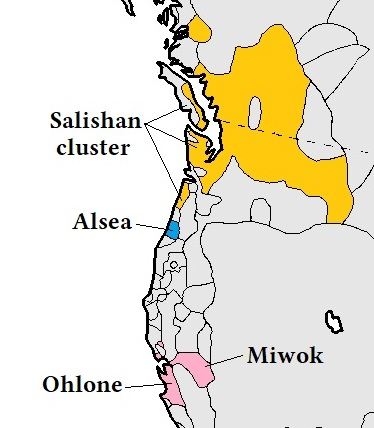
\includegraphics[width=55mm]{WestAmerica-LinLib.jpg}}
\end{figure}


\section{Tunisian Arabic}\label{sec:TunAra}
Metathesis in Tunisian Arabic is described by \cite{kidr86}.
Their discussion begins with the observation that Tunisian Arabic has a process of
phonologically conditioned metathesis (\srf{sec:PhoMet}),
in which the medial CV sequence of a CCVC stem metathesises
before a vowel-initial suffix.
Examples are given in \qf{ex:TunAraMorMet} below.

\begin{exe}
	\ex{CC\sub{2}V\sub{1}C {\ra} CV\sub{1}C\sub{2}C /{\gap}-V \hfill\cite[61]{kidr86}}\label{ex:TunAraMorMet}
	\sn{\gw\begin{tabular}{llcll}
								&Stem							&			&\mc{2}{l}{Suffixed Form}\\
		`palms'			&\it{n\tbr{xa}l}	&{\ra}&\it{n\tbr{ax}l-a}	&`a palm' \\
		`mountain'	&\it{\j\tbr{bə}l}	&{\ra}&\it{\j\tbr{əb}l-i}	&`mountains' \\
		`he wrote'	&\it{k\tbr{tə}b}	&{\ra}&\it{k\tbr{ət}b-u}	&`they wrote' \\
		`month'			&\it{ʃ\tbr{ħa}r}	&{\ra}&\it{ʃ\tbr{aħ}r-iːn}&`two months' \\	
	\end{tabular}}		
\end{exe}

However, there are a number of verbs in which CV {\ra} VC metathesis
alone results in a nominalisation, producing what \citeauthor{kidr86}
call a \it{nomen actionis} (action noun).
Such metathesis only affects words of the shape CCVC.
Examples are given in \qf{ex:TunAraDerMet} below.
%(There is also one example of a metathesis with concurrent apophony of the vowel;
%\it{ħ\tbr{rə}m} `he prohibited' {\ra} \it{ħ\tbr{ar}m} `prohibition'.)

\begin{exe}
	\ex{Nominalising metathesis \hfill\citep[62]{kidr86}}\label{ex:TunAraDerMet}
	\sn{\gw\begin{tabular}{llcll}
										&Verb							&			&Noun&\\
		`he understood'	&\it{f\tbr{hə}m}	&{\ra}&\it{f\tbr{əh}m}		&`understanding'\\
		`he was sick'		&\it{m\tbr{rˁa}ðˁ}	&{\ra}&\it{m\tbr{arˁ}ðˁ}	&`sickness'\\
		`he owned'			&\it{m\tbr{lə}k}		&{\ra}&\it{m\tbr{əl}k}		&`asset'\\
		`he lied'				&\it{k\tbr{ðə}b}		&{\ra}&\it{k\tbr{əð}b}		&`lying'\\
		`he tightened'	&\it{ħ\tbr{sˁa}rˁ}	&{\ra}&\it{ħ\tbr{asˁ}rˁ}	&`act of tightening'\\
		`he blasphemed'	&\it{k\tbr{fɔ}r}		&{\ra}&\it{k\tbr{ɔf}r}		&`blasphemy'\\
		`he prohibited'	&\it{ħ\tbr{rə}m}		&{\ra}&\it{ħ\tbr{ar}m}		&`prohibition'\\
	\end{tabular}}		
\end{exe}

An alternate analysis of the same data would be to identify the nouns as the base
from which verbs are derived by VC {\ra} CV metathesis.
\cite{kidr86} adduce both diachronic evidence
as well as native speaker judgements in favour of their
analysis of metathesis as a nominaliser.

Metathesis is only one of a number of nominalisation strategies in Tunisian Arabic.
Another nominalisation strategy is affixation.
Nominalising affixes include \it{-aːn}, \it{-(j)a},
\it{m(a)-} or a combination of \it{m-{\ldots}-a}.
Examples are given in \qf{ex:TunAraAff} below.
Suffixation with a vowel-initial suffix
also triggers phonologically conditioned metathesis of CCVC roots,
as seen in \qf{ex:TunAraMorMet} above.

\begin{exe}
	\ex{Nominalising affixation \hfill\citep[63f]{kidr86}}\label{ex:TunAraAff}
	\sn{\gw\begin{tabular}{llcll}
										&Verb					&			&Noun										&\\
		`he attached'		&\it{rˁbatˁ}	&{\ra}&\it{rˁabtˁ-\tbr{a}}		&`act of attaching' \\
		`he read'				&\it{qra}			&{\ra}&\it{qraː-\tbr{ja}}			&`reading' \\
		`he blasphemed'	&\it{kfɔr}		&{\ra}&\it{kɔfr-\tbr{aːn}}		&`blasphemy'\footnotemark\\
		`he asked'			&\it{tˁləb}		&{\ra}&\it{\tbr{ma}-tˁləb}		&`request' \\
		`he loved'			&\it{ħabb}		&{\ra}&\it{\tbr{m}-ħabb-\tbr{a}}	&`act of loving' \\
	\end{tabular}}		
\end{exe}
\footnotetext{
Some verbs have multiple nominalising strategies.
The verb \it{kfɔr} `blaspheme' is one such example, either undergoing metathesis,
as shown in \qf{ex:TunAraDerMet}, or suffixation, as shown here in \qf{ex:TunAraAff}.}

Another nominalisation strategy is apophony,
either replacing a short vowel with the equivalent long vowel
or replacing it with a vowel of a different quality.
Examples are given in \qf{ex:TunAraApo} below.

\begin{exe}
	\ex{Nominalising apophony \hfill\citep[64]{kidr86}}\label{ex:TunAraApo}
	\sn{\gw\begin{tabular}{llcll}
									&Verb			&			&Noun				&\\
		`he slept'		&\it{rq\tbr{a}d}&{\ra}&\it{rq\tbr{aː}d}	&`sleep' \\
		`he went mad'	&\it{xb\tbr{ə}l}&{\ra}&\it{xb\tbr{aː}l}	&`going mad' \\
		`he entered'	&\it{dx\tbr{ə}l}&{\ra}&\it{dx\tbr{uː}l}	&`act of entering' \\
		`he swam'			&\it{ʕ\tbr{aː}m}&{\ra}&\it{ʕ\tbr{uː}m}	&`swimming'\\
		`he sold'			&\it{b\tbr{aː}ʕ}&{\ra}&\it{b\tbr{iː}ʕ}	&`(a) sale' \\
	\end{tabular}}		
\end{exe}

The final nominalisation strategy is zero derivation;
that is conversion of a verb into a noun with no phonological change.
Examples are given in \qf{ex:TunAraZerDer} below.

\begin{exe}
	\ex{Zero derivation \hfill\citep[63,65]{kidr86}}\label{ex:TunAraZerDer}
	\sn{\gw\begin{tabular}{lll}
		\it{ʕməl} 	& `he did' {\tl} `deed' \\
		\it{ʕtˁasˁ}	& `sneeze' {\tl} `act of sneezing' \\
		\it{nðˁar} 	& `he saw' {\tl} `seeing' \\
		\it{xbar}		& `he informed' {\tl} `informing' \\
	\end{tabular}}		
\end{exe}

\citet[71]{kidr86} carried out two tests to determine
how productive each of these nominalisation strategies were for CCVC verbs.
In each case metathesis was the most productive nominalisation strategy.

In the first test speakers were presented with ten fictional verbs
and a variety of nominalisations formed according
to each possible process illustrated in \qf{ex:TunAraDerMet}--\qf{ex:TunAraZerDer} above.
Metathesis was the preferred strategy in 8/10 instances
in the first run of this test and was preferred in 9/10 instances in the second run.\footnote{
		The other acceptable nominalisation strategy was suffixation with \it{-aːn}.
		There were also two responses in which either metathesis or suffixation with \it{-aːn}
		were judged acceptable.}

Similar judgements were given for the loan words
\it{nmar} (< French \it{numéroter}) `to number',
\it{mraʃ} (< French \it{marcher}) `to march'
and \it{mrəs} (< French \it{remercier}) `to thank'.
Among loanwords the only exception was \it{bləf} < English \it{bluff},
for which the preferred nominalisation strategy was zero derivation.

The second test \citeauthor{kidr86} carried out
involved choosing either metathesis or zero derivation
as the preferred nominalisation strategy.
In this test 17/18 responses selected metathesis.

In summary, metathesis in Tunisian Arabic is one of several processes
available to nominalise verbs with the structure CCVC.
Metathesis is productive and is the preferred nominalisation strategy.
That metathesis in Tunisian Arabic is associated with other processes
is consistent with the data in Chapter \ref{ch:SynchMet}
in which metathesis is associated with
a large number of additional processes.
%However, in Amarasi most of these processes are consequences of metathesis,
%such as vowel assimilation triggered by metathesis (\srf{sec:VowAss}),
%while in Tunisian Arabic these processes are independent of metathesis,
%with the exception of suffixation triggering metathesis.

\section{Svan}\label{sec:Sva}
Svan is a Kartvelian language of northern Georgia.
Causatives of intransitive verbs are formed in Svan by final VC {\ra} CV metathesis.
Published sources are extremely scarce.
\citet[297]{me97} gives the six examples in \qf{ex:SvaMet} below.
In all six instances metathesis derives a causative from an intransitive verb.\footnote{
		All six examples in \qf{ex:SvaMet} are cited with the prefix \it{li-} of which 
		\citet{me97}, states ``Les exemples ci-dessous sont cités à la forme du nom d’action verbal,
		appelé \emph{masdar}, dont les rôles syntaxiques sont comparables à ceux de l'infinitif du français.'';
		``The examples below are given in the form of a verbal action noun,
		called \emph{masdar}, whose syntactic roles are similar to those of the French infinitive.''}

\begin{exe}
	\ex{Svan causative metathesis \hfill\citep[297]{me97}}\label{ex:SvaMet}
	\sn{\gw\begin{tabular}{llcll}
											&\tsc{intr} 					&			&\tsc{caus}	&\\
		 `go out' 				&\it{li-d\tbr{eg}} 		&{\ra}&\it{li-d\tbr{ge}}		&`extinguish' \\
		 `break (intr.)'	&\it{li-kʷ'\tbr{es'}}	&{\ra}&\it{li-kʷ'\tbr{s'e}}	&`break (tr.)' \\
		 `rot' 						&\it{li-kʷ\tbr{er}} 	&{\ra}&\it{li-kʷ\tbr{re}}		&`make/let rot' \\
		 `come' 					&\it{li-q\tbr{ed}} 		&{\ra}&\it{li-q\tbr{de}}		&`bring, convey' \\
		 `return (intr.)'	&\it{li-t'\tbr{ex}}		&{\ra}&\it{li-t'\tbr{xe}}		&`return (tr.)' \\
		 `get dirty' 			&\it{li-g\tbr{eb}} 		&{\ra}&\it{li-g\tbr{be}}		&`make dirty' \\
	\end{tabular}}		
\end{exe}

\section{Mutsun Ohlone (Costanoan)}\label{sec:Ohl}
Metathesis in the Mutsun variety of Southern Ohlone (a.k.a. Costanoan),
a now extinct language of central California (see \frf{fig:LanWesAmeMorMet}), is described in \cite{ok79}.
The same author also wrote a grammar of the language published as \citet{ok77}.
In both instances data was drawn from material gathered in the
early twentieth century from the last fluent speaker.

Verbs in Mutsun have two stems, called the primary stem and the derived stem.
The main difference between each stem is that the derived stem is consonant final,
while the primary stem can be either vowel final or consonant final.
\cite{ok79} identifies seven types of stems of which stem types II, IV and VII show metathesis.
These three stem types are given in \trf{tab:MutPriDerVerSte}
(the fourth stem type is poorly attested in the data).
In all cases the derived stem is formed from the primary
stem by metathesis of the final VC sequence.

\begin{table}[h]
	\caption[Mutsun primary and derived verb stems]{Mutsun primary and derived verb stems \citep[125]{ok79}}\label{tab:MutPriDerVerSte}
	\centering
		\begin{tabular}{rrllll} \lsptoprule
					&Primary 							&Derived 						& \mc{2}{l}{Examples} 				&Gloss\\ \midrule
			II	&CVCV\sub{2}ːC\sub{3}	&CVCC\sub{3}V\sub{2}& \it{pasiːk-}	& \it{paski-}	&`to greet, visit'\\
			IV	&CVːCV\sub{2}C\sub{3}	&CVCC\sub{3}V\sub{2}& \it{liːwak-}	& 						&`to hide nearby'\\
			VII	&CVCːV\sub{2}C\sub{3}	&CVCC\sub{3}V\sub{2}& \it{liʧːej-}	& \it{liʧje-}	&`to stand'\\
			\lspbottomrule
		\end{tabular}
\end{table}

In most cases the use of each stem is either phonologically or morphemically conditioned.
A phonologically conditioned use is found before suffixes which begin with a consonant cluster
in which case VC {\ra} CV metathesis occurs to prevent a cluster of three consonants surfacing.
Examples include \it{pas\tbr{iːk}} `visit' + \it{-jni} `to come to'
{\ra} \it{pas\tbr{ki}jni} `come to visit'
and \it{liʧː\tbr{ej}} `to stand' + \it{-hte} \tsc{perfective} {\ra}
\it{liʧ\tbr{je}hte} `already assumed a standing position'.

Likewise, word final consonant clusters are disallowed in Mutsun.
As a result derived stems are used before suffixes consisting of a single consonant.
One example is \it{sotː\tbr{er}} `stick out' + \it{-j} \tsc{imperative}
{\ra} \it{sot\tbr{re}j} `stick out [your foot]!' \citep[125]{ok79}.

However, there are also some CV(C) suffixes which only occur with primary stems
and other CV(C) suffixes which only occur with derived stems.
This is a case of morphemically conditioned metathesis (\srf{sec:MorpheConMet}),
in which metathesis is a partial exponent of the morphological
category signalled by the suffix.

Suffixes which take primary stems include the reciprocal suffix \it{-mu}
and the reflexive suffix \it{-pu},
as seen in \it{hiːwo} `scold (s.o.)' + \it{-mu} \tsc{recp} {\ra} \it{hiːwomu} `(they) quarrel' 
and \it{matːal} `face down' + \it{-pu} \tsc{refl} {\ra} \it{matːalpu} `put oneself face down'.
One suffix which takes the derived stem and thus triggers metathesis is \it{-nu} `positional causative',
as seen in \it{matː\tbr{al}} `face down' + \it{-nu} {\ra} \it{mat\tbr{la}nu}
`put (s.o.) face down (into a prone position)' \citep[126]{ok79}.

The morphological function of metathesis comes about because the derived stem
is used in isolation as a non-past tense
and there are a number of cognate nouns
which take the primary stem.
Examples are given in \qf{ex:MutDerMet} below.

\begin{exe}
	\ex{Mutsun derivational metathesis \hfill\citep[127]{ok79}}\label{ex:MutDerMet}
	\sn{\gw\begin{tabular}{llll}
		 					 			&Noun								&Verb							& \\
		 `a cough' 			&\it{toːh\tbr{er}}	&\it{toh\tbr{re}} & `to cough' \\
		 `flute' 				&\it{lulː\tbr{up}}	&\it{lul\tbr{pu}} & `to play the flute' \\
		 `goose' 				&\it{laːl\tbr{ak}}	&\it{lal\tbr{ka}} & `gather geese' \\
		 `nest'					&\it{heːs\tbr{en}}	&\it{hes\tbr{ne}} & `make a nest' \\
		 `pozole (stew)'&\it{pos\tbr{ol}}		&\it{pos\tbr{lo}} & `to make pozole (stew)' \\
	\end{tabular}}		
\end{exe}

Given that Mutsun is now extinct, it is hard to tell exactly how productive metathesis was.
However, the occurrence of the Spanish loanword \it{posol} `pozole (stew)'
with both metathesised  and unmetathesised forms indicates that metathesis was productive.
It is likely that VC {\ra} CV metathesis in Mutsun was used to derive verbs from nouns.\footnote{
		Mutsun \it{posol} is a loan from Spanish \it{pozole}, itself a loan from Nahuatl \it{pozolli}.
		The final final /e/ of the Spanish form has been re-analysed in Mutsun as 
		the object case suffix; \it{posoːl-e} \citep[127, fn.14]{ok77}.}

%The main similarity between the Mutsun Ohlone data and the Amarasi data
%is in the distribution of metathesis.
%In both instances metathesis is phonological
%in some contexts and morphological in others.
\section{Sierra Miwok}\label{sec:SieMiw}
Sierra Miwok is a language of central California
(see \frf{fig:LanWesAmeMorMet}) related to Ohlone (\srf{sec:Ohl}).
My summary of Sierra Miwok metathesis is based on the description in \cite{fr51}.
Like Ohlone, each verb in Sierra Miwok has multiple stems.
There are three derived stems in Sierra Miwok formed from one of
four different shapes of the primary (underlying) stem.
These different shapes are summarised in \trf{tab:SieMiwVerSte}.
on the next page.

\begin{table}[h]
	\caption[Sierra miwok verb stems]{Sierra miwok verb stems\su{†} \citep[94f]{fr51}}\label{tab:SieMiwVerSte}
	\centering
		\begin{threeparttable}[b]
			\begin{tabular}{rccccl}\lsptoprule
					&Primary						&Second				&Third				&Fourth				&\\ \midrule
			I		&CVC\tbr{V}ː\tbr{C}	&CVCVCː				&CVCːVC				&CVC\tbr{CV} 	&\\
					&\it{tujaːŋ-}				&\it{tujaŋː-}	&\it{tujːaŋ-}	&\it{tujŋa-}	& `to jump'\\
			II	&CVC\tbr{CV}				&CVC\tbr{VC}ː	&CVCː\tbr{VC}	&CVCCV 				&\\
					&\it{wɨkt̪ɨ-}				&\it{wɨkɨt̪ː-}	&\it{wɨkːɨt̪-}	&\it{wɨkt̪ɨ-}	&`to burn'\\
			III	&CVCːV							&CVCVʔː				&CVCː\tbr{Vʔ}	&CVC\tbr{ʔV}	&\\
					&\it{hamːe}					&\it{hameʔː-}	&\it{hamːeʔ-}	&\it{hamʔe-}	&`to bury'\\
			IV	&CVːC								&CVCː					&CVCː\tbr{Vʔ}	&CVC\tbr{ʔV}	&\\
					&\it{luːʃ-}					&\it{luʃː-}		&\it{luʃːuʔ-}	&\it{luʃʔu-}	&`to win'\\ \lspbottomrule
			\end{tabular}
			\begin{tablenotes}
				\item [†] Stress in Sierra Miwok falls on the first heavy syllable;
									either VCC, VːC or VCː \citep[7]{fr51}.
									Because it is predictable, I do not indicate its presence in this section.
			\end{tablenotes}
		\end{threeparttable}
\end{table}

The shape of each derived stem is consistent across all four verb classes,
with the exception of the second stem of class IV verbs.
The second derived stem has the shape CVCVCː,
the third stem CVCːVC and the fourth stem CVCCV.

In all cases the final C-slot is filled by a glottal stop
when the root has only two consonants.
Similarly, when the root has only a single vowel the final V-slot is filled
by /u/ after back rounded vowels,
and by /ɨ/ after all other vowels.
Both these facts can be seen with the primary stem \it{luːʃ-} `to win'
with the CVCːVC third stem \it{luʃː\tbr{uʔ}-}
with the final vowel and consonant
occurring to fill the otherwise empty V-slot and C-slot.

Final consonant-vowel metathesis is found in three cases;
between the primary stem of verb class I and the fourth stem,
with VC {\ra} CV metathesis,
and between the primary stem of verb class II
and the second and third derived stems,
with CV {\ra} VC metathesis.
It is also possible to analyse the epenthetic glottal stop as undergoing metathesis
in the third and fourth stems of class III verbs and class IV verbs.

As in Mutsun, some cases of metathesis in Sierra Miwok 
are instances of phonologically conditioned metathesis.
Before a CC initial suffix the fourth stem is used,
thereby avoiding a cluster of three consonants.
One example is the class I stem \it{pol\tbr{a}ː\tbr{ŋ}}
`to stagger' + \it{-jnɨ} \tsc{desiderative}
{\ra} \it{pol\tbr{ŋa}jnɨ} \citep[116]{fr51}.

There are also many instances of morphemically conditioned metathesis
with different suffixes of the same phonological shape occurring with different stems.
Such instances are extremely numerous and I do not provide examples here.

In addition there are also instances
in which metathesis alone serves a a morphological function.
For instance, one nominalisation strategy
for class I verbs is to use the fourth stem.
Examples are given in \qf{ex:SieMiwVerMet} below,
in which nouns are cited with the \tsc{subjective} suffix \it{-ʔ}

\newpage
\begin{exe}
	\ex{Sierra Miwok verbalising metathesis \hfill\citep[149]{fr51}}\label{ex:SieMiwVerMet}
	\sn{\gw\begin{tabular}{lrcll}
								&Verb												&			&Noun									&\\
		`to relate'	&\it{ʔut̪\tbr{e}ː\tbr{n}-}		&{\ra}&\it{ʔut̪\tbr{ne}-ʔ}		&`myth, tale' \\
		`to tell'		&\it{koy\tbr{o}ː\tbr{w}-}		&{\ra}&\it{koy\tbr{wo}-ʔ}		&`words, speech' \\
		`to run'		&\it{hɨw\tbr{a}ː-\tbr{t̪}-}	&{\ra}&\it{hɨw\tbr{t̪a}-ʔ}		&`race' \\
		`to play'		&\it{ʔaw\tbr{i}ː-\tbr{n}-}	&{\ra}&\it{ʔaw\tbr{ni}-ʔ}		&`game' \\
		`to live'		&\it{ʔu{\tS}ːu-}						&{\ra}&\it{ʔu{\tS}ʔu-ʔ}			&`health, well-being: year' \\
		`to come'		&\it{ʔɨnːɨ-}								&{\ra}&\it{ʔɨnʔɨ-ʔ-}				&`way, journey' \\
		`to eat'		&\it{ʔɨwːɨ-}								&{\ra}&\it{ʔɨwʔɨ-ʔ}					&`food' \\
	\end{tabular}}
\end{exe}

The processes in Mutsun Ohlone and Sierra Miwok have much in common,
as might be expected from related languages.
However, in Mutsun Ohlone VC {\ra} CV metathesis is a  verbaliser
while in Sierra Miwok the same process is a nominaliser.

%The Sierra Miwok data has two similarities to Amarasi.
%Firstly, metathesis in Sierra Miwok is phonologically conditioned
%in some contexts and morphological in others.
%Secondly, metathesis in Sierra Miwok interacts with empty C-slots and empty V-slots.
%In Sierra Miwok empty C-slots and V-slots are filled by default segments
%which then metathesise with each other or with specified segments.
%
%In Amarasi, empty C-slots also occur and metathesise with filled V-slots
%triggering processes such as consonant insertion and vowel assimilation.
%The way empty C-slots interact with Amarasi metathesis is discussed in \srf{sec:ThePhoRul}
%and evidence for positing empty C-slots is presented in \srf{sec:EmpCSlo}.

\section{Alsea}\label{sec:Als}
Alsea is a now extinct language of the Oregon coast (see \frf{fig:LanWesAmeMorMet}).
The only consonants which participate in metathesis in Alsea are sonorants.
Metathesis in Alsea is mostly morphemically conditioned (\srf{sec:MorpheConMet}).
One suffix which triggers metathesis is the third person object imperative suffix \it{-t}.
Examples are given in \qf{ex:AlsMorphemicMet} below
in which the metathesised stems on the right
can be compared with unmetathesised counterparts on the left.

\begin{exe}
	\ex{Alsea morphemically conditioned metathesis \hfill\citep[8f]{bu07}}\label{ex:AlsMorphemicMet}
		\sn{\stl{0.3em}\gw\begin{tabular}{lrll}
		`had closed it'				&\it{t\tbr{mú}s-sa-nχ}		&\it{t\tbr{úm}s-t}		&`close it!'\\
		`agreed to it'				&\it{t'\tbr{má}s-sal-tχ}	&\it{t'\tbr{ám}s-t}		&`finish it!'\\
		`had been sliding'		&\it{st\tbr{lá}k-sal-tχ}	&\it{st\tbr{ál}k-t}		&`slide it!'\\
		`is packing'					&\it{ʦu\tbr{lá}q'n-tχ}		&\it{ʦu\tbr{ál}q'n-t}	&`pack it!'\\
		`is close to shore'		&\it{t\tbr{lú}qʷ'-χ}			&\it{t\tbr{úl}qʷ'-t}	&`bring it close to shore!'\\
		`is in act of hiding'	&\it{p\tbr{yá}χ-aw-tχ}		&\it{p\tbr{áy}X-t}		&`hide it!'\\
		`had pierced'					&\it{qɬ\tbr{jú}t-sal}			&\it{qɬ\tbr{új}-t}		&`prick him!'\\
	\end{tabular}}		
\end{exe}

That this metathesis is not conditioned by the phonological shape of the suffix
is shown by the contrast between suffixes with an identical form,
one of which triggers metathesis while the other does not.
The intransitive imperative suffix \it{-χ} triggers metathesis
while the completive realis \it{-χ} suffix does not trigger metathesis.
Examples are given in \qf{ex:AlsMorphemicMet2} below.

\begin{exe}
	\ex{Alsea morphemically conditioned metathesis \hfill\citep[8f]{bu07}}\label{ex:AlsMorphemicMet2}
	\sn{\gw\begin{tabular}{lrll}
											&\tsc{cmpl.rl}			&\tsc{intr.imp}		& \\
		`dances with them'&\it{k\tbr{ná}χ-χ}	&\it{k\tbr{án}χ-χ}&`dance with them!' \\
		`are lying in bed'&\it{ʦ\tbr{nú}s-χ}	&\it{ʦ\tbr{ún}s-χ}&`lie down!' \\
		`is hiding'				&\it{p\tbr{já}χ-χ}	&\it{p\tbr{áj}χ-χ}&`hide!' \\
		`is floating'			&\it{ʦp\tbr{jú}t-χ}	&\it{ʦp\tbr{új}t-χ}&`float!' \\
	\end{tabular}}		
\end{exe}

In addition to such morphemically conditioned metathesis there are also hints that
Alsea had a process of morphological metathesis which signalled aspect.
\cite{bu07} gives three potential examples, given in \qf{ex:AlsMorMet} below.

\begin{exe}
	\ex{Alsea morphological metathesis \hfill\citep[10]{bu07}}\label{ex:AlsMorMet}
	\sn{\stl{0.4em}\gw\begin{tabular}{lrll}
		`keep it shut!'		&\it{t\tbr{mú}s-t}			&\it{t\tbr{úm}s-t}			&`shut it!' \\
		`is stretched out'&\it{ʦɬ\tbr{já}q-tχ}		&\it{ʦɬ\tbr{áj}q-tχ}		&`made it straight' \\
		`was (not) 				&\it{ʦqʷ\tbr{ná}qʷ-ɬn-χ}&\it{ʦqʷ\tbr{án}qʷ-ɬn-χ}&`was being \\ \hhline{~}
		\hp{`}overtaken'	&												&												&\hp{`}overtaken' \\
	\end{tabular}}		
\end{exe}

However, such examples come only from elicitation
with no indication of the context in which they could be used.
Nonetheless, given the (historic) location of Alsea,
bordering on the area in which Salishan languages are spoken (see \frf{fig:LanWesAmeMorMet}),
it would not be surprising if Alsea had 
also developed a morphological process of morphological metathesis to mark aspect.\footnote{
		Alsea is not considered genealogically related to the Salishan languages.}
\section{Salishan}\label{sec:Sal}
The Salishan languages are a family of languages spoken in the Pacific Northwest,
around the western border of the United States of America and Canada (see \frf{fig:LanWesAmeMorMet}).
Most Salishan languages are either critically endangered or have recently become extinct.
I discuss metathesis in three Salishan varieties, all of which belong to the Coast Salish group.
These varieties include two varieties of Straits Salish:
Saanich (\srf{sec:Saa}) and Klallam (\srf{sec:Kla}),
as well as a Central Salishan variety, Halkomelem (\srf{sec:Hal}).
All are spoken in the immediate vicinity of Southern Vancouver island.

In each of these Salishan varieties metathesis signals the so-called
actual aspect described by \citet[215]{thth69}
as an ``action or state in effect at a particular moment''.
\citeauthor{thth69} compare this actual aspect to the Slavic imperfective
as well as the English \it{be {\ldots}-ing} progressive.
I refer to this aspect as the imperfective \tsc{(ipfv)} throughout this section.

In each Salishan language metathesis is only one of a number of processes used to form the imperfective.
Other processes include reduplication, infixation,
glottalisation, apocope, and apophony (among others).
Which process applies can usually, though not always, be predicted based
on the phonological shape of the perfective stem.

\subsection{Saanich}\label{sec:Saa}
I begin my discussion of Salishan metathesis with Saanich,
a variety of Straits Salish.
Saanich metathesis is described in \cite{mo86,mo89}.
Several different processes operate in Saanich to form the imperfective aspect.
These processes include infixation, reduplication, and metathesis.
Which of these processes operates is determined by the shape of the stem,
with the goal being to achieve a CVCC word structure for the imperfective.
In addition to these processes
all non-initial sonorants are glottalised in imperfective forms.

Metathesis occurs in two environments.
Firstly, when the root contains no vowels
and is suffixed with a vowel-initial suffix,
metathesis of this vowel and the root final consonant
occurs to form the imperfective.
Examples are given in \qf{ex:CC-V->CVC} below,
with the `control transitive' suffix \it{-ət}.

\begin{exe}
	\ex{Saanich C\sub{1}C\sub{2}-V\sub{1}{\ldots} {\ra} C\sub{1}V\sub{1}C\sub{2}{\ldots} \hfill\citep[97]{mo89}}\label{ex:CC-V->CVC}
	\sn{\gw\begin{tabular}{llrcll}
			Root				&							&\tsc{pfv}									&			&\tsc{ipfv}							&\\
		\it{{\rt}q'p'}&`patch it'		&\it{xʷ-q'\tbr{p'-\'ə}t}			&{\ra}&\it{xʷ-q'\tbr{\'əp'}t}	&`patching it' \\
		\it{{\rt}sq'}	&`tear it'		&\it{s\tbr{q'-\'ə}t}	&{\ra}&\it{s\tbr{\'əq'}t}			&		`tearing it' \\
		\it{{\rt}sχ}	&`push it'		&\it{s\tbr{χ-\'ə}t}		&{\ra}&\it{s\tbr{\'əχ}t}			&`pushing it' \\
		\it{{\rt}ʃʧ'}	&`whip it'		&\it{ʃ\tbr{ʧ'-\'ə}t}	&{\ra}&\it{ʃ\tbr{\'əʧ'}t}			&`whipping it' \\
		\it{{\rt}tkʷ}	&`break it'		&\it{t\tbr{kʷ-\'ə}t}	&{\ra}&\it{t\tbr{\'əkʷ}t}			&`breaking it' \\
		\it{{\rt}tqʷ}	&`tighten it'	&\it{t\tbr{qʷ-\'ə}t}	&{\ra}&\it{t\tbr{\'əqʷ}t}			&`tightening it' \\
		\it{{\rt}t's}	&`break it'		&\it{t'\tbr{s-\'ə}t}	&{\ra}&\it{t'\tbr{\'əs}t}			&`breaking it' \\
%		\it{{\rt}θkʷ}	&`straighten it out'&\it{θ\tbr{kʷ\'ə}t}		&{\ra}&\it{θ\tbr{\'əkʷ}t}			&`straightening it out' \\
		\it{{\rt}θχ}	&`shove it'		&\it{θ\tbr{χ-\'ə}t}		&{\ra}&\it{θ\tbr{\'əχ}t}			&`shoving it' \\
	\end{tabular}}		
\end{exe}

Similarly CCəC roots form the imperfective
by metathesis of the second consonant with the following vowel.
Examples are given in \qf{ex:CCVC->CVCC} below.
Only stems containing the vowel [ə] undergo metathesis in Saanich.

\newpage
\begin{exe}
	\ex{Saanich C\sub{1}C\sub{2}ə\/C\sub{3} {\ra} C\sub{1}ə\/C\sub{2}C\sub{3} \hfill\citep[93,97]{mo86,mo89}}\label{ex:CCVC->CVCC}
	\sn{\stl{0.4em}\gw\begin{tabular}{llrcll}
			Root									&									&\tsc{pfv}									&			&\tsc{ipfv}					&\\
		\it{{\rt}t\su{θ}'ɬəkʷ'}	&`pinch'					&\it{t\su{θ}'\tbr{ɬ\'ə}kʷ'}	&{\ra}&\it{t\su{θ}'\tbr{\'əɬ}kʷ'}	&`pinching' \\
		\it{{\rt}t͜ɬ'pəχ}				&`scatter'				&\it{t͜ɬ'\tbr{p\'ə}χ}				&{\ra}&\it{t͜ɬ'\tbr{\'əp}χ}		&`scattering' \\
		\it{{\rt}t͜ɬ'kʷ'ət}			&`extinguish it'	&\it{t͜ɬ'\tbr{kʷ'\'ə}t}			&{\ra}&\it{t͜ɬ'\tbr{\'əkʷ'}t}	&`extinguishing it' \\
		\it{{\rt}θɬəqʷ}					&`pierce it'			&\it{θ\tbr{ɬ\'ə}qʷ}					&{\ra}&\it{θ\tbr{\'əɬ}qʷ}			&`piercing it' \\
	\end{tabular}}		
\end{exe}

With stems of other shapes, reduplication or infixation of /ʔ/ occurs.
The process of reduplication copies the first consonant of a CVC root and
places it after the first vowel.
Reduplication applies \it{``[{\ldots}] when stress is on the root and the root either
1) stands alone as a stem by itself or
2) is followed by a suffix beginning with a consonant.''} \citep[95]{mo89}.
Examples are given in \qf{ex:C1VC->C1VC1C} below.
Predictable schwas are transcribed with a breve [ə̆].

\begin{exe}
	\ex{Saanich C\sub{1}\'VC\sub{2} {\ra} C\sub{1}\'VC\sub{1}C\sub{2} \hfill\citep[95]{mo89}}\label{ex:C1VC->C1VC1C}
	\sn{\stl{0.4em}\gw\begin{tabular}{lllcll}
			Root					&							&\tsc{pfv}			&		&\tsc{ipfv}					&\\
		\it{{\rt}qen'}	&`it's stolen'&\it{sqén'}			&\ra&\it{qéqə̆n'}				&`he's stealing' \\
		\it{{\rt}t\su{θ}'eʔ}	&`be on top'	&\it{t\su{θ}'éʔ}			&\ra&\it{t\su{θ}'ét\su{θ}'ə̆ʔ}		&`riding (a horse)' \\
		\it{{\rt}qʷəl'}	&`say'				&\it{qʷ\'əl'}		&\ra&\it{qʷ\'əqʷə̆l'}		&`saying (sth.)' \\
		\it{{\rt}kʷul}	&`school'			&\it{s-kʷúl}		&\ra&\it{s-kʷúkʷə̆l'}		&`going to school' \\
		\it{{\rt}ɬikʷ'}	&`trip'				&\it{ɬíkʷ'-sən}	&\ra&\it{ɬíɬə̆kʷ'-sən'}	&`tripping' \\
	\end{tabular}}		
\end{exe}

In other cases a glottal stop is infixed after the first vowel.
This infixation can also be accompanied by other
various phonological processes such as apophony.
Examples of infixation which do not involve any additional complications
are given in \qf{ex:C1VC->C1VqC} below.

\begin{exe}
	\ex{Saanich C\sub{1}VC\sub{2}(VC) {\ra} C\sub{1}V\it{ʔ}C\sub{2}(VC) \hfill\citep[98]{mo89}}\label{ex:C1VC->C1VqC}
	\sn{\stl{0.4em}\gw\begin{tabular}{lllcll}
			Root								&							&\tsc{pfv}	&			&\tsc{ipfv}					&\\
	%	\it{{\rt}ʔit\su{θ}'}	&`get dressed'&\it{ʔít\su{θ}'əN}		&{\ra}&\it{ʔí\<ʔ\>t\su{θ}'əN'}		&`getting dressed' \\
		\it{{\rt}ʔeʧ'}		&`wipe it'&\it{ʔéʧ'-ət}		&{\ra}&\it{ʔé\<ʔ\>ʧ'-ət}		&`wiping it' \\
		\it{{\rt}ʔiɬən}		&`eat'		&\it{ʔíɬən}			&{\ra}&\it{ʔí\<ʔ\>ɬən'}			&`eating' \\
		\it{{\rt}ʧaqʷ'}		&`sweat'	&\it{ʧáqʷ'-əŋ}	&{\ra}&\it{ʧá\<ʔ\>qʷ'-əŋ'}	&`sweating' \\
		\it{{\rt}weqəs}		&`yawn'		&\it{wéqəs}			&{\ra}&\it{wé\<ʔ\>qəs}			&`yawning' \\
		\it{{\rt}xʷit}		&`jump'		&\it{xʷít-əŋ}		&{\ra}&\it{xʷí\<ʔ\>t-əŋ'}		&`jumping' \\
		\it{{\rt}ʔamət}		&`sleep'	&\it{ʔámət}			&{\ra}&\it{ʔá\<ʔ\>m'ət}			&`sleeping' \\
	\end{tabular}}		
\end{exe}

In Saanich metathesis is one of several
processes which occurs to form the imperfective.
Other processes include reduplication and infixation.
Which process operates is determined by the phonological shape of the stem,
with the goal of forming a CVCC word shape in the imperfective.

It may be possible at an abstract level to analyse surface metathesis in Saanich
as an artefact of other phonological processes.
This is particularly so given that Saanich metathesis only affects roots with schwa /ə/.
This is the approach taken by \cite{de74} for similar data in the
closely related language Lummi (discussed in \srf{sec:EpeApo}),
in which metathesis is analysed as resulting from
stress shift with subsequent deletion of unstressed vowels.

\subsection{Klallam}\label{sec:Kla}
Klallam is very closely related to Saanich
and the data on Klallam metathesis is similar to that in Saanich.
Metathesis in Klallam is described by \cite{thth69}.
As in Saanich, there are a number of process for forming the imperfective aspect in Klallam.
These processes include infixation of /ʔ/, metathesis, and reduplication.

Examples of verbs which form the imperfective by metathesis
are given in \qf{ex:KlaCVC->CCV} below.
All words are cited with the control suffix \it{-t}.
Predictable schwas are transcribed with a breve [ə̆].

\begin{exe}
	\ex{Klallam CCV {\ra} CVC \hfill\citep[216]{thth69}}\label{ex:KlaCVC->CCV}
	\sn{\gw\begin{tabular}{lrcll}
								&\tsc{pfv}									&			&\tsc{ipfv}							&\\
			`tie up'	&\it{q'\tbr{xʷí}-t}					&{\ra}&\it{q'\tbr{íxʷ}-t}			&`tying up'\\
			`scratch'	&\it{χ\tbr{ʧ'í}-t}					&{\ra}&\it{χ\tbr{íʧ'}-t}			&`scratching'\\
			`restrain'&\it{q\tbr{q'í}-t}					&{\ra}&\it{q\tbr{íq'}-t}			&`restraining'\\
			`shoot'		&\it{ʧ\tbr{kʷú}-t}					&{\ra}&\it{ʧ\tbr{úkʷ}-t}			&`shooting'\\
			`throw'		&\it{ʧ\tbr{ʃú}-t}						&{\ra}&\it{ʧ\tbr{ús}-t}				&`throwing'\\
			`shatter'	&\it{t'\tbr{ʦ\'ə}-t}				&{\ra}&\it{t'\tbr{\'əʦ}-t}		&`shattering'\\
			`grasp'		&\it{t͜ɬ'\tbr{kʷ\'ə}-t}			&{\ra}&\it{t͜ɬ'\tbr{\'əkʷ}-t}	&`grasping'\\
			`swallow'	&\it{ŋə̆\tbr{q'\'ə}-t}				&{\ra}&\it{ŋ\tbr{\'əq'}-t}		&`swallowing'\\
			`pick up'	&\it{mə̆\tbr{kʷ'\'ə}-t}			&{\ra}&\it{m\tbr{\'əkʷ'}-t}		&`picking up'\\
			`burn'		&\it{ʧ\tbr{qʷ\'ə}-t}				&{\ra}&\it{ʧ\tbr{\'əqʷ}-t}		&`burning'\\
			`tear'		&\it{ʧ\tbr{χ\'ə}-t}					&{\ra}&\it{ʧ\tbr{\'əχ}-t}			&`tearing'\\
			`chop'		&\it{q'}\it{\tbr{mˀ\'ə}-t}	&{\ra}&\it{q'\tbr{\'əmˀ}-t}		&`chopping'\\
			`bite'		&\it{ʦ'}\it{ə̆\tbr{ŋˀ\'ə}-t}	&{\ra}&\it{ʦ'\tbr{\'əŋˀ}-t}		&`biting'\\
			`put in water'&\it{mə̆\tbr{t\'ə}qʷ-t}	&{\ra}&\it{m\tbr{\'ət}qʷ-t}		&`putting in water'\\
			`pour'		&\it{kʷ\tbr{jˀ\'ə}-t}				&{\ra}&\it{kʷ\tbr{\'əjˀ}-t}		&`pouring'\\
	\end{tabular}}		
\end{exe}

Other verbs form the imperfective by infixation of the glottal stop after the first vowel.
Some examples are given in \qf{ex:KlaC1VC->C1VqC} below.

\newpage
\begin{exe}
	\ex{Klallam C\sub{1}VC\sub{2}(VC) {\ra} C\sub{1}VʔC\sub{2}(VC) \hfill\citep[216]{thth69}}\label{ex:KlaC1VC->C1VqC}
		\sn{\gw\begin{tabular}{llcll}
								&\tsc{pfv}			&			&\tsc{ipfv}					&\\
			`wipe'		&\it{ʔáʧ'-t}		&{\ra}&\it{ʔá\<ʔ\>ʧ'-t}		&`wiping' \\
			`nudge'		&\it{ʦ'út'-t}		&{\ra}&\it{ʦ'ú\<ʔ\>t'-t}		&`nudging' \\
			`make'		&\it{ʧáʧ-t}			&{\ra}&\it{ʧá\<ʔ\>ʧ-t}			&`making' \\
			`blow'		&\it{púxʷ-t}		&{\ra}&\it{pú\<ʔ\>xʷ-t}		&`blowing' \\
			`set fire'&\it{húnə̆-t}		&{\ra}&\it{hú\<ʔ\>nə̆-t}		&`setting fire' \\
	\end{tabular}}		
\end{exe}

Metathesis and glottal stop infixation
are the two most common ways of forming the imperfective in Klallam.
Another strategy is reduplication,
as seen in \it{jáʔ-t} {\ra} \it{jájəʔ-t} `prepare'.
(Reduplication also involves a change in the quality of the root vowel.)

There are also verbs which combine glottal stop infixation with
either reduplication or metathesis.
When metathesis and infixation are combined,
the glottal stop infix ends up after the first consonant.
Examples are given in \qf{ex:KlaCVC->CqCV}.

\begin{exe}
	\ex{Klallam C\sub{1}VC\sub{2} {\ra} C\sub{1}ʔC\sub{2}V \hfill\cite[216]{thth69}}\label{ex:KlaCVC->CqCV}
	\sn{\gw\begin{tabular}{lrcll}
								&\tsc{pfv}					&		&\tsc{ipfv}								&\\
			`beat'		&\it{qʷ'\tbr{úʧ}-t}	&\ra&\it{qʷ'ə̆\<ʔ\>\tbr{ʧú}-t}	&`beating'\\	
			`inflate'	&\it{s\tbr{új}ə̆-t}	&\ra&\it{sə̆\<ʔ\>\tbr{jú}-t}		&`inflating'\\
			`command'	&\it{sá-t}					&\ra&\it{sə̆\<ʔ\>á-t}					&`commanding'\\
	\end{tabular}}		
\end{exe}

In Klallam metathesis is one of at least three
strategies used to form the imperfective.
The fact that a variety of roots -- not only those with medial schwa --
undergo metathesis to form the imperfective
poses a challenge for analyses of the Klallam data
in which metathesis is viewed as an artefact of
other processes, such as epenthesis and vowel deletion,
as discussed by \cite[540]{blga98}.
Regarding such an analysis, \cite[217]{thth69} state:

\begin{quote}
This treatment [an analysis involving true metathesis]
has the advantage of not requiring the setting up of special
hypothetical base forms like *čukʷut [*ʧukʷut `shoot'],
with actual and non-actual forms derived by vowel deletion,
or positing special stress patterns inserting vowels in different positions with relation to root consonants.
The current popular tendency to resort to such abstractions
(even where they may be well motivated in historical-comparative terms)
is at variance with objective consideration
of the facts of particular language structures
and tends to obstruct our efforts to understand how languages change
and to obscure phenomena important in the consideration of typological similarities. %\citep[217]{thth69}
\end{quote}		

\subsection{Halkomelem}\label{sec:Hal}
My summary of metathesis in Halkomelem is based on that provided by \cite{ur11},
who describes the Hul'q'umi'num' (Vancouver Island) dialect.
As in the other Salishan languages discussed,
metathesis in Halkoemelem is one of several processes used to form the imperfective.
Other processes include vowel apophony, reduplication, and vowel deletion.
Which process applies is (mostly) determined by the phonological shape of the verb.

Metathesis occurs when the verb root contains two obstruents followed by a vowel.
Examples are given in \qf{ex:HalCCV{\ra}CVC} below.
As in Saanich, non-initial sonorants
are additionally glottalised in the imperfective.

\begin{exe}
	\ex{Halkomelem C\sub{1}C\sub{2}V {\ra} C\sub{1}VC\sub{2} \hfill (\citet{hu78} in \citealp[477f]{ur11})}\label{ex:HalCCV{\ra}CVC}
	\sn{\stl{0.4em}\gw\begin{tabular}{lrcll}
										&\tsc{pfv}					&		&\tsc{ipfv}					&\\
		`break it'			&\it{p\tbr{qʷá}-t}	&\ra&\it{p\tbr{áqʷ}-t}	&`breaking it' \\
		`break it'			&\it{t'\tbr{qʷ'á}-t}&\ra&\it{t'\tbr{áqʷ'}-t}&`breaking it' \\
		`pull it'				&\it{xʷ\tbr{kʷ'á}-t}&\ra&\it{xʷ\tbr{ákʷ'}-t}&`pulling it' \\
		`tear/split it'	&\it{s\tbr{q'é}-t}	&\ra&\it{s\tbr{éq'}-t}	&`tearing/splitting it' \\
	\end{tabular}}		
\end{exe}

\citet{ur11} compares metathesis to a process of stress shift and schwa insertion,
viewing metathesis as a specific instances of this latter process.
Examples of imperfectives formed by stress shift
and epenthesis are given in \qf{ex:HalCCV->C@C@}.

\begin{exe}
	\ex{Halkomelem C\sub{1}C\sub{2}V {\ra} C\sub{1}ə́C\sub{2}ə \hfill \citep[478]{ur11}}\label{ex:HalCCV->C@C@}
	\sn{\stl{0.4em}\gw\begin{tabular}{lrcll}
												&\tsc{pfv}				&		&\tsc{ipfv}					&\\
		`tell him/her'			&\it{ʦse-t}				&\ra&\it{ʦə́sə-t}				&`telling him/her' \\
		`put it near'				&\it{tse-t}				&\ra&\it{tə́sə-t}				&`putting it near' \\
		`count stitches'		&\it{kʷ'ʃáləs-t}	&\ra&\it{kʷ'ə́ʃəl'əs-t }	&`counting stitches' \\
		`slice out a piece	&\it{ɬʦ'áləs-t}		&\ra&\it{ɬə́ʦ'əl'əs-t}		&`slicing out a piece \\ \hhline{~}
		\hp{`}of weaving'		&									&		&										&\hp{`}of weaving' \\
	\end{tabular}}		
\end{exe}

When the verb begins with CVC where neither consonant is a laryngeal,
or if the verb begins with an obstruent followed by schwa,
the first CV is reduplicated as a prefix to form the perfective.
If the vowel of the reduplicant is not schwa, stress falls on this vowel
and other vowels are reduced to schwa.
If the vowel of the reduplicant is schwa, stress falls on the second vowel.

\newpage
\begin{exe}
	\ex{Halkomelem C\sub{1}V\sub{1}C\sub{2} {\ra} C\sub{1}V\sub{1}C\sub{1}əC\sub{2} \hfill\citep[474f]{ur11}}\label{ex:HalRed}
	\sn{\gw\begin{tabular}{lrcll}
									&\tsc{pfv}		&		&\tsc{ipfv} & \\
		`cut it' 			&\it{ɬíʦ'ət}	&\ra&\it{ɬíɬəʦ'ət}		&`cutting it'\\
		`fight' 			&\it{kʷíntəl}	&\ra&\it{kʷíkʷən'təl}	&`fighting'\\
		`topple down' &\it{jeq'}		&\ra&\it{jéj'əq'}			&`toppling down'\\
		`get near' 		&\it{təs}			&\ra&\it{tətə́s}				&`getting near'\\
		`break' 			&\it{t'əqʷ'}	&\ra&\it{t'ət'ə́qʷ' }	&`breaking'\\
		`stretched taut'&\it{θəkʷ'}	&\ra&\it{θəθ\'əkʷ'}		&`stretching'\\
	\end{tabular}}		
\end{exe}

When the root begins with a sonorant (L) followed by schwa,
the imperfective is reported to be formed by CV reduplication
with subsequent reduction of the initial sonorant to /h/.
Stress falls on the reduplicant and the following schwa is deleted,
resulting in surface metathesis when comparing the perfective and imperfective forms.
%Any non-schwas in the root are reduced to schwa after reduplication.
Examples are given in \qf{ex:HalRed2} below.

\begin{exe}
	\ex{L\sub{1}əC\sub{2} {\ra} h\'əL\sub{1}C\sub{2} \hfill(\citet{hupe95} in \citealp[475]{ur11})}\label{ex:HalRed2}
	\sn{\stl{0.3em}\gw\begin{tabular}{lrcll}
											&\tsc{pfv}				&		&\tsc{ipfv} & \\
		`fill it' 				&\it{l\'əʦ'ət}		&\ra&\it{h\'əl'ʦ't}			&`filling it'\\
		`pile hay' 				&\it{m\'əkʷels}		&\ra&\it{h\'əm'kʷəl's}	&`piling hay'\\
		`bounce a cradle' &\it{n\'əkʷəjəł}	&\ra&\it{h\'ən'kʷəjəł}	&`bouncing a cradle'\\
		`drift						&\it{w\'əqʷ'ətəm}	&\ra&\it{h\'əw'qʷ'ətəm'}&`drifting \\ \hhline{~}
		\hp{`}downstream'	&									&		&										&\hp{`}downstream' \\
	\end{tabular}}		
\end{exe}

The remaining two ways of forming the imperfective
are apophony and schwa deletion.
Both are found with tri-consonantal roots,
the latter only when the suffix is \it{-m}.
Examples are given in \qf{ex:HalApo} below.

\begin{exe}
	\ex{Halkomelem apophony/schwa deletion \hfill\citep[475f]{ur11}}\label{ex:HalApo}
	\sn{\gw\begin{tabular}{lrcll}
										&\tsc{pfv}						&		&\tsc{ipfv} 					& \\
		`slurp it'			&\it{ɬəp't\su{θ}'-t}	&\ra&\it{ɬep't\su{θ}'-t}	&`slurping it'\\
		`seek'					&\it{səwq'}						&\ra&\it{sew'q'}					&`seeking'\\
		`fall apart'		&\it{ʦ'át'əqʷ'əm}			&\ra&\it{ʦ'át'qʷ'əm'}			&`falling apart'\\
		`fall (leaves)'	&\it{t͜ɬ'épəχəm}				&\ra&\it{t͜ɬ'épχəm'}				&`falling (leaves)'\\
	\end{tabular}}		
\end{exe}

In Halkomelem metathesis is one of several processes used to form the imperfective.
Other processes include stress shift, reduplication, apophony, and apocope.
Which process applies is predictable based on the phonological shape of the root.
Metathesis affects roots which contain two obstruents.
%
%In the Salishan languages CV {\ra} VC metathesis is one of several
%processes used to form the imperfective from the perfective.
%The main similarities between the Salishan data and the Amarasi data
%is that in both instances metathesis is associated with a large number of other processes.
%In Amarasi these processes are best analysed as being triggered by metathesis,
%while in the Salishan languages these other processes may have given rise to metathesis (\srf{sec:OriMorMet}).

\chapter{Selected Amarasi texts}\label{app:SelAmaTex}

\counterwithin{exx}{section}

\section{Preface}
In this appendix I present four Amarasi texts,
three from the Kotos dialect which is the focus of this
book and one from Ro{\Q}is.
The Kotos texts include a narrative about a recent event (\S\ref{sec:DeaNahBan}),
a myth about the beginning of the world (\S\ref{sec:MooHit}),
and a conversation (\S\ref{sec:CarCrash}).
The Ro{\Q}is text (\srf{sec:GatBanFam}) is a short life history.

Each sentence/intonation unit is given twice.
The first line is sequentially numbered gives an orthographic transcription.
The second line is numbered according to its time in the recording.
This line is given in phonemic transcription,
which is followed by the gloss and a free translation.

Glossing follows the same conventions used throughout this book,
with the exception that the third person singular genitive
suffix \ve{-n} is glossed \tsc{3gen} in the Kotos texts
and \tsc{3psr;sg.psm} in the Ro{\Q}is text (\srf{sec:RoqPoss}).

The only instances of metathesis which are indicated in the glosses
are those which have a morphological meaning:
M-forms of nouns modified by an attributive modifier (Chapter \ref{ch:SynMet})
and U-forms of vowel final verbs and other word classes
which take discourse driven U-forms (Chapter \ref{ch:DisMet}).
Non-morphological M-forms and U-forms
can be detected by comparing the phonemic transcription in the top line
with the corresponding underlying forms in the second line.

\renewcommand{\N}{\tsc{3gen}}
\section{The death of Nahor Bani}\label{sec:DeaNahBan}
\subsection{Metadata}

\wg\begin{tabular}{lL{.67\textwidth}}
File-name:					& aaz20130928{\_}01\\
Archive-link:				& \url{http://catalog.paradisec.org.au/collections/OE1/items/aaz20130928_01}\\
Original Name:			& aaz-20130928-1-HeronimusBani- CeritaNahorBaniMati\\
Language:						& Amarasi [aaz] \\
Dialect:						& Kotos; Koro{\Q}oto hamlet \\
Location:						& Nekmese{\Q}, Amarasi Selatan, Kupang \\
Date:								&	28/09/2013\\
Speaker(s):					& Heronimus Bani\\
Recorded by: 				& Heronimus Bani, Owen Edwards\\
Transcribed by:			& Heronimus Bani\\
Interlinear by:			& Owen Edwards \\
Indonesian/Kupang:	& Heronimus Bani\\
Free English by:		& Charles E. Grimes\\
Genre:							& narrative\\
Summary:						& Roni relates a disagreement over where recently
										deceased Nahor Bani should be buried\\
%Length:						& 2.51\\
%Notes:							& \\
\end{tabular}


\subsection{Notes}
Heronimus Bani relates about a disagreement over where recently deceased
Nahor Bani should be buried.
Most families want to bury their loved
ones in their yard so they can care for the grave.
The government has been pushing for everyone
to be buried in designated community graveyards
(Indonesian \it{T.P.U.} = \it{tempat pemakaman umum})
``for public health reasons''.
Culturally in Timor, the \ve{nitu} `spirit of the dead' can disturb,
disrupt, cause sickness, crop failure, etc. to the living if angry or neglected.
Monitoring and taking good care of the grave
is one way to show respect and prevent bad
things happening to good people.\footnote{
		Thanks go to Charles Grimes for the cultural background to this text.}

\newpage
\subsection{The text}
\begin{exe}

\ex{\ve{Neno ia aam Nahor Bani in nmaet.}}
\exi{0.02}{\glll	neno ia aam Nahor Bani iin n-maet\\
									neno ia ama Nahor Bani ini n-mate \\
									day {\ia} father{\M} Nahor Bani {\iin} \n-die \\
						\glt	`Today father Nahor Bani died.'}

\ex{\ve{Oras in nmate te,}}
\exi{0.06}{\glll	oras iin n-mate =te\\
									oras ini n-mate =te\\
									time {\iin} \n-die{\U} ={\te}\\
						\glt	`When he died, ' }

\ex{\ve{in aan moen jes, kaan ee nai{\Q} Fanu,}}
\exi{0.11}{\glll	iin aan moon\j=ees, kaan-n=ee naiʔ Fanu\\
									ini anah mone=esa kana-n=ee naiʔ Fanu \\
									{\iin} child{\M} male=one name-{\N}={\ee} {\naiq} Fanu\\
						\glt	`one of his sons named Fanu' }

\ex{\ve{anhain nain nopu.}}
\exi{0.17}{\glll	a|n-hain n-ain nopu\\
									{\a}n-hani n-ani nopu \\
									\a\n-dig \n-before hole \\
						\glt	\lh{\a}`had dug the grave beforehand.' }

\ex{\ve{Re{\Q} uaba ma too mfaun re{\Q} kuan ii naan ii nak am: nopu mnanun.}}
\exi{0.20}{\begin{xlist}
	\ex{\glll	reʔ uaba =m too mfaun	\\
						reʔ uaba =ma too mfaun	\\
						{\req} speech =ma populace many \\}

	\ex{\glll	reʔ kuan=ii naan-n=ii n-aka =m ehh nopu mnanu-n\\
						reʔ kuan=ii nana-n=ii n-ak =ma {} nopu mnanu-n \\
						{\req} village={\ii} inside-{\N}={\ii} \n-say =and {} hole deep-{\N}\\
			\glt	`of which it was said, (by) many people who (are) in this village, (they) said the grave was deep.}
	\end{xlist}}

\newpage
\ex{\ve{In ka nhain je ruum aah fa te, nhani nrair je te, nrame.}}
\exi{0.30}{\begin{xlist}
	\ex{\glll	iin ka= n-haan\j=ee ruum=aah =fa =te\\
						ini ka= n-hani=ee ruum=aha =fa =te\\
						{\iin} {\ka}= \n-dig={\eeV} plain=just ={\fa} ={\te} \n-dig \n-finish={\eeV} ={\te} \n-plaster{\U}\\
			\glt `He did not just dig it plainly (i.e. with plain dirt walls),'}

	\ex{\glll	n-hani n-raar\j=ee =t n-rame\\
						n-hani n-rari=ee =te n-rame\\
						\n-dig \n-finish={\eeV} ={\te} \n-plaster{\U}\\
			\glt	`(when) he finished digging it, he plastered it (with concrete).' }
\end{xlist}}

\ex{\ve{Nraem je reko-reko.}}
\exi{0.33}{\glll	n-raam\j=ee reko{\tl}reko\\
									n-rame=ee reko{\tl}reko \\
									\n-plaster={\eeV} {\frd}good \\
						\glt `He plastered it properly.' }

\ex{\ve{Onaim re{\Q} natfeek onai te, are{\Q} amahonit, ana{\Q}a prenat, too mfaun ein, neem nabuan am,}}
\exi{0.36}{\begin{xlist}
	\ex{\glll	{onai =m}, reʔ na-tfeek {onai =te} areʔ amahonit, anaʔaprenat\\
						{onai =ma} reʔ na-tfeka {onai =te} areʔ amahonit anaʔaprenat\\
						and.so {\req} \na-cut.off and.then every parent official\\}
	
	\ex{\glll	too mfaun=ein, neem na-bua=n =am\\
						too mfaun=eni nema na-bua=n =ma\\
						populace many={\ein} {\nema} \na-gather={\einV} =and\\
			\glt `So, when (the breath of the deceased) was cut off (= died) then all the parents/clan elders,
						(local) government officials, and many of the populace came and gathered'\footnote{
								The form \ve{amahonit} `parent' (with variant \ve{mahonit}) is a lexicalised nominalisation
								from \ve{a\=/ma\=/honi\=/t} {\at}-{\ma}\=/born-{\at}.
								The phrase \ve{anaʔaprenat} `official' is a lexicalised historic nominalisation 
								from \ve{a-naʔa-t} {\at}-hold-{\at} + \ve{prenat} `govern'.}}
\end{xlist}}

\newpage
\ex{\ve{he na{\Q}uab ein neu re{\Q} he tpafa{\Q} ai{\Q} tsuba ma, on re{\Q} mee?}}
\exi{0.48}{\begin{xlist}
	\ex{\glll	he na-ʔuab=ein n-eu reʔ he a|t-pafaʔ aiʔ t-suba =ma\\
						he na-ʔuaba=eni n-eu reʔ he {\a}t-pafaʔ aiʔ t-suba =ma\\
						{\he} \na-speak={\einV} \n-{\eu} {\req} {\he} \a\t-protect or \t-bury{\U} =and\\}

	\ex{\glll on reʔ mee\\
						on reʔ mee\\
						like {\reqt} how\\
			\glt `to discuss about how we are going protect or bury (the body) and how (are we going to go about this)?' }
\end{xlist}}

\ex{\ve{Oat hau gui on re{\Q} mee, ai{\Q} noup paarn ii on re{\Q} mee?}}
\exi{0.57}{\glll	oat haagw=ii on reʔ mee, aiʔ noup paar-n=ii, on reʔ mee\\
									ote hau=ii on reʔ mee aiʔ nopu para-n=ii on reʔ mee\\
									cut{\M} wood={\ii} like {\reqt} how or hole{\M} short-{\N}={\ii} like {\reqt} how\\
						\glt `How should the cutting of the wood (for the casket) be?
									Or, how short should the hole (for the grave) be? ' }

\ex{\ve{Ma nopu mnaun{\Q} ii te, on re{\Q} mee?}}
\exi{1.02}{\glll	ma nopu mnaunʔ=ii =t on reʔ mee\\
									ma nopu mnanuʔ=ii =te on reʔ mee\\
									and hole deep={\ii} ={\te} like {\reqt} how\\
						\glt `and how deep should the hole be?' }

\ex{\ve{Onai te, re{\Q} nai{\Q} Faun gui, fee{\Q}n ii uab ii,}}
\exi{1.06}{\glll	{onai =te} reʔ naiʔ Faaŋgw=ii, feeʔn=ii uab=ii, \\
									{onai =te} reʔ naiʔ Fanu=ii feʔen=ii uaba=ii \\
									then {\reqt} {\naiq} Fanu={\ii} earlier={\ii} speech={\ii} \\
						\glt `So then this Fanu (that I) mentioned earlier,' }

\newpage
\ex{\ve{nak on in ka natonan fa ana{\Q}a preent ein ii, ai{\Q} mahoint ein ii, neu re{\Q} in nhain nain nopu.}}
\exi{1.10}{\glll	n-ak on iin ka= na-tona=n =fa anaʔapreent=ein=ii aiʔ \hspace{10mm} mahoint=ein=ii n-eu reʔ iin n-hain n-ain nopu\\
									n-ak on ini ka= na-tona=n =fa anaʔaprenat=eni=ii aiʔ {} amahonit=eni=ii n-eu reʔ ini n-hani n-ani nopu \\
									\n-say {\on} {\iin} {\ka}= \n-tell={\ein} ={\fa} official={\ein}={\ii} or {} parents={\ein}={\ii} \n-{\eu} {\reqt} {\iin} \n-dig \n-before hole \\
						\glt	`(it was) said that he had not told the government officials,
									or the clan leaders that he had dug the grave beforehand,' }

\ex{\ve{Ai{\Q} in nmesel anrari, nrame nrari.}}
\exi{1.18}{\glll	aiʔ iin n-\sf{mesel} a|n-rari, n-rame n-rari\\
									aiʔ ini n-\sf{mesel} {\a}n-rari n-rame n-rari\\
									or {\iin} \n-grave.cover \a\n-finish{\U} \n-plaster \n-finish{\U}\\
						\glt `or that he had built the grave cover and had plastered it with cement.' }

\ex{\ve{In nmeerk on.}}
\exi{1.22}{\glll	iin n-meerk=oo-n\\
									ini n-merak=oo-n \\
									{\iin} \n-quiet=\oo-{\N}\\
						\glt	`He kept himself quiet.' }

\ex{\ve{Onaim ana{\Q}a preent ein nok nai{\Q} Fanu in taatf eni,}}
\exi{1.22}{\glll	{onai =m} anaʔapreent=ein n-ok naiʔ Fanu iin taat-f=eni\\
									{onai =ma} anaʔaprenat=eni n-oka naiʔ Fanu ini tata-f=eni\\
									and.so official={\ein} {\n-\ok} {\naiq} Fanu {\iin} eSi-{\F}={\ein\U}\\
						\glt	`So the government officials and Fanu’s elder siblings' }

\ex{\ve{aam Simson nok aam Ayub, nema ntean onai te,}}
\exi{1.28}{\glll	aam Simson n-ok aam Ayup nema n-tea=n {onai =t}\\
									ama Simson n-oka ama Ayup nema n-tea=n {onai =te}\\
									father{\M} Simson {\n-\ok} father{\M} Ayub {\nema} \n-until={\einV} and.then\\
						\glt	`Mr. Simson (Samson) and Mr. Ayub (Job) came' }

\newpage
\ex{\ve{nak on na{\Q}uab ein am ma,}}
\exi{1.32}{\glll	n-ak on na-ʔuab=ein =ama\\
									n-ak on na-ʔuaba=eni =ma\\
									\n-say like \na-speak={\einV} =and\\
						\glt	`thinking like they were going to discuss, and' }

\ex{\ve{sin he nnaon nsuban on bare {\Q}bua{\Q} re{\Q} nteek ee nak T.P.U.}}
\exi{1.34}{\begin{xlist}
	\ex{\glll	siin he n-nao=n n-suba=n on, bare ʔ-bua-ʔ \\
						sini he n-nao=n n-suba=n on bare ʔ-bua-ʔ\\
						{\siin} {\he} \n-go={\einV} \n-bury={\einV} {\on} place {\qq}-gather-{\qq}\\
			\glt `they were going to go bury him at the place (where graves are) gathered'}

	\ex{\glll	reʔ n-teek=ee n-ak, \sf{tee} \sf{pee} \sf{uu}\\
						reʔ n-teka=ee n-ak \sf{tee} \sf{pee} \sf{uu}\\
						{\req} \n-call={\eeV} {\n-\ak} T P U\\
			\glt `which is called T.P.U. (\it{tempat pemakaman umum} = public burial place)'}
\end{xlist}}

\ex{\ve{Hei, maans ee nmaeb ia te,}}
\exi{1.41}{\glll	heeʔ maans=ee n-maeb ia =te\\
									heeʔ manas=ee n-mabe ia =te\\
									hey sun={\ee} \n-afternoon {\ia} ={\te}\\
						\glt	`Well, late this afternoon' }

\ex{\ve{uab ii nfain suir jeen, nasurin. }}
\exi{1.43}{\glll	uab=ii n-fain suur\j=een, na-suri=n.\\
									uaba=ii n-fani suri=ena na-suri=n\\
									speech={\ii} \n-turn collide={\een} \na-collide={\einV}\\
						\glt	`the discussion had turned into a clash, they were at cross purposes.'}

\ex{\ve{Nasurin neu re{\Q} aam Fanu in neekn ii he nsuub nabaar re{\Q} kintal natuin}}
\exi{1.47}{\begin{xlist}
\ex{\glll	na-suri=n n-eu reʔ aam Fanu iin neek-n=ii \\
					na-suri=n n-eu reʔ ama Fanu ini neka-n=ii \\
					\na-collide={\einV} \n-{\eu} {\reqt} father{\M} Fanu {\iin} feelings-{\N}={\ii}\\}

\ex{\glll he n-suub na-baar reʔ \sf{kintal} na-tuin\\
					he n-suba  na-bara reʔ \sf{kintal} na-tuin\\
					{\he} \n-bury \na-forever {\reqt} yard \na-because\\
		\glt `They were at odds over father Fanu's desire to permanently bury (him), in the yard because' }
\end{xlist}}

\ex{\ve{in aamf ii es anrenu ma nhain re{\Q} nopu,}}
\exi{1.54}{\glll	iin aam-f=ii esa n-renu =ma n-hain reʔ nopu\\
									ini ama-f=ii esa n-renu =ma n-hani reʔ nopu \\
									{\iin} father-{\F}={\ii} one \n-order{\U} =and \n-dig {\reqt} hole \\
						\glt	`his father was the one who ordered (him), and he had dug the hole,' }

\ex{\ve{anraem je nok.}}
\exi{1.58}{\glll	a|n-raam\j=ee n-ok\\
									{\a}n-rame=ee n-oka\\
									\a\n-plaster={\eeV} {\n-\ok}\\
						\glt	\lh{\a}`and had also plastered it' }

\ex{\ve{Onaim ana{\Q}a preent ein nmatoof ein et re{\Q} nee nok are{\Q} mahoint eni ma}}
\exi{2.01}{\glll	{onai =m} anaʔapreent=ein n-ma-toof=ein et reʔ nee n-ok areʔ mahoint=eni =m\\
									{onai =ma} anaʔaprenat=eni n-ma-tofa=eni et reʔ nee n-oka areʔ mahonit=eni =ma\\
									and.so official={\ein} \n-\mak-quarrel={\ein} {\et} {\req} {\nee} {\n-\ok} every parents={\ein\U} =and\\
						\glt	`So (consequently) the government officials, they argued there with all the clan elders, and…' }

\ex{\ve{nuuk tuaf eni, nai{\Q} Fanu nok are{\Q} in tataf}}
\exi{2.05}{\glll	nuuk tua-f=eni, naiʔ Fanu n-ok areʔ iin tata-f\\
									nuka tua-f=eni naiʔ Fanu n-oka areʔ ini tata-f\\
									grief{\M} person-{\f}={\ein\U} {\naiq} Fanu {\n-\ok} every {\iin} eSi-{\f}\\
						\glt	`the bereaved, Mr. Fanu and with all his elder siblings, ' }

\ex{\ve{es-es ate nok in fee in mone,}}
\exi{2.09}{\glll	es{\tl}esa =t n-ok iin fee iin mone\\
									es{\tl}esa =te n-oka ini fee ini mone \\
									{\prd}one ={\te} {\n-\ok} {\iin} wife {\iin} husband \\
						\glt	`each one (of them) with his wife or her husband,' }

\ex{\ve{nasurin am ka tahiin he suubt ii on re{\Q} mee.}}
\exi{2.11}{\glll	na-suri=n =am ka= ta-hiin he suub-t=ii on reʔ mee\\
									na-suri=n =ma ka= ta-hini he suba-t=ii on reʔ mee\\
									\na-collide={\einV} =and {\ka}= {\ta}-know {\he} bury-{\at}={\ii} like {\reqt} how\\
						\glt	`they were at odds and we didn't know where we would bury him.' }

\ex{\ve{Ana{\Q}a preent ein naiti {\Q}niimk ein am ka tahiin he}}
\exi{2.16}{\glll	anaʔapreent=ein n-aiti ʔniim-k=ein =am ka= ta-hiin he\\
									anaʔaprenat=eni n-aiti ʔnima-k=eni =am ka= ta-hini he\\
									official={\ein} \n-lift hand-{\k}={\ein} and {\ka}= {\ta}-know {\he}\\
						\glt	`The government officials lifted their hands (= didn't want to have anything more to do with it) and we didn't know whether ' }

\ex{\ve{urusan he reek haef, are{\Q} tobiru on tiis raur gui he on re{\Q} mee?}}
\exi{2.28}{\begin{xlist}
	\ex{\glll	\sf{urusan} reʔ he reek hae-f \\
						\sf{urusan} reʔ he rekaʔ hae-f \\
						dealings {\req} {\he} order{\M} messenger-{\f} \\
			\glt `arrangements like sending messengers out (with news of the death),' }

	\ex{\glll areʔ tobiru on ahh tiis raargw=ii he on reʔ mee\\
						areʔ tobiru on {} tisi raru=ii he on reʔ mee\\
						every work {\on} {} pour{\M} palm.wine={\ii} {\he} like {\reqt} how\\
			\glt `every detail that had to be attended to, like (the ceremonial) pouring palm-wine, was going to happen how?'}
\end{xlist}}

\ex{\ve{Maut hena{\Q} tatniin sin.}}
\exi{2.33}{\glll	maut henaʔ ta-tniin =siin\\
									maut henaʔ ta-tnina =sini \\
									let {\he} {\ta}-listen {\siin}\\
						\glt `We really should listen to them.' (Deliberately vague.)}

\ex{\ve{Aam Nahor Bani nmaet, in raisn ii {\Q}tet-teta{\Q} kuun.}}
\exi{2.35}{\begin{xlist}
	\ex{\glll	aam Nahor Bani n-maet\\
						ama Nahor Bani n-mate \\
						father{\M} Nahor Bani \n-die \\}

	\ex{\glll	iin rais-n=ii ʔtet{\tl}tetaʔ kuu-n\\
						ini rasi-n=ii ʔtet{\tl}tetaʔ kuu-n\\
						{\iin} issue-{\N}={\ii} {\prd}different alone-{\N}\\
			\glt	`Father Nahor Bani died, and his issue (relating to his death) is entirely different by itself.' }
\end{xlist}}

\end{exe}

\section{Moo{\Q}hitu{\Q}}\label{sec:MooHit}

\subsection{Metadata}
\wg\begin{tabular}{lL{.67\textwidth}}
File-name:					& aaz20120715{\_}04\\
Archive-link:				& \url{http://catalog.paradisec.org.au/collections/OE1/items/aaz20120715_04}\\
Original Name:			& aaz-20120715-4-Nekmese-KusnawiBani-2\\
Language:						& Amarasi [aaz] \\
Dialect:						& Kotos; Koro{\Q}oto hamlet \\
Location:						& Nekmese{\Q}, Amarasi Selatan, Kupang \\
Date:								& 15/07/2015 \\
Speaker(s):					& Taniel Feni, Kusnawi Bani, Heronimus Bani\\
Recorded by: 				& Daniel Kaufman, Heronimus Bani\\
Transcribed by:			& Yedida Ora\\
Interlinear by:			& Owen Edwards \\
Indonesian/Kupang:	& Yedida Ora\\
Free English by:		& Owen Edwards\\
Genre:							& folk-tales\\
Summary:						& Story of Moo{\Q}hitu{\Q}, a mythical snake who created the world\\
Video:							& \url{https://www.youtube.com/watch?v=Z_2D9WhYuuM&list=PLcXFPx-z7B0q_2Ns3iYHigEY77DG4kXSU&index=15}\\
\end{tabular}

\subsection{Notes}
The original recording contains a number of separate stories.
I present here only the first story:
the story of Moo{\Q}hitu{\Q}.
This may be a conflation of two separate myths.
The first is a creation myth about how Moo{\Q}hitu{\Q}, a snake-like being,
separates the sky, land and sea.
The second myth is about how a python copulated with women
and is, perhaps, an explanation for the origin of men.
In Timorese thought the human world cannot exist without
women, who are the source of life.
This leaves unexplained the origin of men.

The information in the myth is incredibly dense
in parts and certain information is left unexplained and/or
assumed to be known by the hearers.
Footnotes provide additional explanations
as well as possible alternate readings.

\subsection{The text}
\begin{exe}

%\ex{\ve{Neno naa re{\Q} paha{\gap}{\Q}piin ii,}}
%\exi{0.00}{\glll	neno naa reʔ paha{\gap}ʔpiin-n=ii\\
%									neno naa reʔ paha{\gap}ʔpina-n=ii\\
%									day {\naa} {\reqt} land{\gap}below-{\N} ={\ii}\\
%						\glt	`At that time the world{\ldots}'}

%\ex[R:]{\ve{mee, mee, mee,}
%				\glt `Hey, wait.'}

%\ex[T:]{\ve{Oi, oi oi oi}
%				\glt `Oh.'}

%\ex[R:]{\ve{\sf{Yep.}}
%			\glt `Yep (start).'}

\ex{\ve{Neno naa pah-a{\Q}pinan ia, ankobub on bare mese{\Q}.}}
\exi{0.05}{\glll	neno naa paha{\gap}ʔpina-n ia a|n-kobub on bare meseʔ \\
									neno naa paha{\gap}ʔpina-n ia {\a}n-kobub on bare meseʔ \\
									day {\naa} land below-{\N} {\ia}	\a\n-piled.up {\on} place one \\
						\glt	`At that time this world was all piled up in one place' }

\ex{\ve{Ka nmui{\Q} fa mainuan.}}
\exi{0.10}{\glll	ka= n-muiʔ =fa maanuan\\
									ka= n-muʔi  =fa mainuan  \\
									{\ka}= \n-exist ={\fa} open \\
						\glt	`there was no openness/space.' }

\ex{\ve{Ka nmui{\Q} fa oe.}}
\exi{0.13}{\glll	ka= n-muiʔ =fa oe\\
									ka= n-muʔi  =fa oe\\
									{\ka}= \n-exist ={\fa} water\\
						\glt	`There was no water.' }

\ex{\label{ex:0.14}\ve{{\Q}Aa{\Q} oe ji nmees, ka tiit fa auf meto{\Q}.}}\footnote{
				Line \qf{ex:0.14}: The meaning of initial phonetic [ʔaːʔ] is currently unclear.
				It may be from the root \ve{{\rt}aʔa} `ritual speech, poetic speech' and
				could, perhaps, mean something like `I am telling it according to tradition'.
				In some other varieties of Meto \ve{{\rt}aʔa} simply means `speak, talk'.}
\exi{0.14}{\glll	ʔ-aaʔ oo\j=ii n-mees ka= tiit =fa auf metoʔ\\
									ʔ-aʔa oe=ii n-mese ka= tita =fa afu metoʔ\\
									\q-speak water={\ii} \n-alone {\ka}= exist ={\fa} ground{\M} dry\\
						\glt	`I say, there was only water, there was no dry ground.'}

\ex{\label{ex:0.17}\ve{Afu ma neno nmanaa{\Q}.}}
\exi{0.17}[K:]{\glll	afu =m neno n-ma-naaʔ\\
											afu =ma neno n-ma-naʔa \\
											ground =and sky \n-\mak-hold \\
								\glt	`The ground and sky held on to one another.' \footnote{
													Line \qf{ex:0.17} is spoken by Kusnawi Bani.}}

\newpage
\ex{\ve{Afu ma neno nmanaa{\Q}. Meis{\Q}ookn ii nnaa{\Q}.}}
\exi{0.18}[T:]{\glll	afu =m neno n-ma-naaʔ meisʔookn=ii n-naaʔ\\
											afu =ma neno n-ma-naʔa  meisʔokan=ii n-naʔa \\
											ground =and sky \n-\mak-hold dark={\ii} \n-hold \\
								\glt	`The ground and sky held on to one another, darkness held (fast).' }

\ex{\label{ex:0.20}\ve{Tapi re{\Q} kauna{\Q} ia, in nmoni nbi oe ji naan ii.}}
\exi{0.20}{\begin{xlist}
	\ex{\glll	\sf{tapi} ahh reʔ kaunaʔ ia \\
						\sf{tapi} {} reʔ kaunaʔ ia \\
						but ahh {\req} snake {\ia} \\}
	\ex{\glll	iin n-moni n-bi oo\j=ee naan-n=ii, \\
						ini n-moni n-bi oe=ee nana-n=ii \\
						{\iin} \n-live \n-loc water={\ee} inside-{\N}={\ii} \\
			\glt	`but as for this snake, he was living inside the water,'}\footnote{
								Line \qf{ex:0.20}:	The snake is Moo{\Q}hitu{\Q}.}
\end{xlist}}

\ex{\ve{Noki-noki te, in naskeke nfena nhake ma,}}
\exi{0.24}{\gll	noki-noki =te iin na-skeke n-fena n-hake =ma\\
									eventually ={\te} {\iin} \na-suddenly \n-rise \n-stand{\U} =and\\
						\glt	`after a while, he suddenly stood up and' }

\ex{\ve{in nfeen es mee te neon gui natsiri{\Q}, natsiri{\Q}, sampai in ntea re{\Q} aat neno nee msa{\Q}, in natuin ee ma,}}\label{ex:0.27}
\exi{0.27}{\begin{xlist}
	\ex{\glll	iin, iin n-feen es mee =t nee{\ng}gw=ii na-tsiriʔ na-tsiriʔ \\
						ini ini n-fena  es mee =te neno=ii na-tsiriʔ na-tsiriʔ \\
						{\iin} {\iin} \n-rise {\et} where ={\te} sky={\ii} \n-spread \n-spread \\
			\glt	`as he went up to somewhere, the sky kept spreading and spreading (upwards)'\footnote{
							Lines \qf{ex:0.27} and \qf{ex:0.34} explain how Moo{\Q}hitu{\Q}
							pushed up the sky, thus separating it from the water.}}

	\ex{\glll	\sf{sampe} iin n-tea reʔ aat neno nee msaʔ\\
						\sf{sampe} ini n-tea reʔ ata neno nee msaʔ \\
						until {\iin} \n-up.to {\req} up sky {\nee} also \\
			\glt `until when he arrived at where the top of the sky also is,'}

	\ex{\glll	iin na-tuin=ee =ma\\
						ini na-tuin=ee =ma\\
						{\iin} \n-follow={\eeV} =and\\
			\glt `he followed it and,'}

\end{xlist}}

\newpage
\ex{\ve{Anhake {\Q}roo-roo =te, es naa neon goe na{\Q} anmana{\Q}a ma,}}\label{ex:0.34}
\exi{0.34}{\begin{xlist}
	\ex{\glll	a|n-hake ʔro{\tl}roo =t \\
						n-hake ʔro{\tl}roo =te \\
						\n-stand {\prd}far ={\te} \\}
	\ex{\glll	es naa nee{\ng}gw=ee naʔ a|n-ma-naʔa =ma	\\
						es naa neno=ee naʔ n-ma-naʔa =ma	\\
						{\et} {\naa} sky={\ee} then \n-\mak-hold{\U} =and\\
			\glt	`when he had stood up for a long time, at that place
							only then the sky held fast (in relation to him) and,' }
\end{xlist}}

\ex{\ve{na{\Q} nsanu nfani kre{\Q}o-kre{\Q}o ma nfani nbi in baran.}}
\exi{0.37}{\begin{xlist}
	\ex{\glll	naʔ n-sanu n-fani kreʔo{\tl}kreʔo =ma\\
						naʔ n-sanu n-fani kreʔo{\tl}kreʔo =ma\\
						then \n-descend \n-return {\frd}a.bit =and\\}
	\ex{\glll	n-fani n-bi iin bara-n\\
						n-fani n-bi ini bara-n\\
						\n-return \n-{\bi} {\iin} place-{\N}\\
			\glt	`then (he) went back down bit by bit and returned to his place'}
\end{xlist}}

\ex{\ve{Nfani nbi in baarn ii. In baarn ee et oe je nanan.}}
\exi{0.40}{\begin{xlist}
	\ex{\glll	n-fani n-bi iin baar-n=ii \\
						n-fani n-bi ini bara-n=ii \\
						\n-return \n-{\bi} {\iin} place-\N={\ii}  \\}
	\ex{\glll	in baar-n=ee et oo\j=ee nana-n\\
						in bara-n=ee et oe=ee nana-n\\
						{\iin} place-\N={\ee} {\et} water={\ee} inside-{\N}\\
			\glt	`(He) went back to his place. His place was inside the water.'}
\end{xlist}}

\ex{\ve{Nbi-bi oe je naan ee onai te, anmo{\Q}e ma npoi jeen anbi meto{\Q}.}}
\exi{0.43}{\begin{xlist}
	\ex{\glll	n-bi{\tl}bi oo\j=ee naan-n=ee {onai =te}\\
						n-ni{\tl}bi oe=ee nana-n=ee {onai =te}\\
						\n-{\prd}loc water={\ee} inside\N={\ee} then\\
			\glt	`after he had been in the water for a while then,'}
	\ex{\glll	a|nmoʔe =ma npoo\j=ena n-bi metoʔ\\
						{\a}n-moʔe =ma n-poi=ena n-bi metoʔ \\
						{\a}\n-do{\U} and \n-exit={\een} \n-{\bi} dry \\
			\glt \lh{\a}`(he) made (dry land) and went out onto dry land,'}
\end{xlist}}

\ex{\ve{Npoi nbi meot{\Q} ee onai te, in ka nmui{\Q} fa bare he natua ma,}}\label{ex:0.47}
\exi{0.47}{\begin{xlist}
	\ex{\glll	n-poi n-bi meotʔ=ee {onai =te}\\
						n-poi n-bi metoʔ=ee {onai =te}\\
						\n-exit \n-{\bi} dry={\ee} then\\}
	\ex{\glll	iin ka= n-muiʔ =fa bare he na-tua =m\\
						ini ka= n-muʔi =fa bare he na-tua =ma\\
						{\iin} {\ka}= \n-exist ={\fa} place {\he} \na-live =and\\
			\glt	`having gone out onto the dry land, he didn't have a place to live and,' }
\end{xlist}}

\ex{\ve{he natua te, baer mainuan.}}
\exi{0.51}{\glll	he na-tua =te he-- baer mainuan\\
									he na-tua =te {} bare mainuan\\
									{\he} \n-live top {} place{\M} open\\
						\glt	`he would (have to) live in an open place,' }

\ex{\ve{Natua te, baer ko{\Q}u.}}
\exi{0.53}{\glll	na-tua =te baer koʔu\\
									na-tua =te bare koʔu \\
									\na-live ={\te} place{\M} big \\
						\glt	`live in a big place,' }

\ex{\ve{Akhirnya, naim naan baer jes am namaika{\Q} nbi Smara{\Q} tunan.}}\label{ex:0.57}
\exi{0.57}{\begin{xlist}
	\ex{\glll	\sf{ahirɲa} ahh n-aim naan baar\j=esa =m namaikaʔ an--,  \\
						\sf{ahirɲa} {} n-ami naan bare=esa =ma na-maikaʔ {} \\
						in.the.end {} \n-look.for {\naan} place={\es} =and \na-stay {}  \\
			\glt `in the end, (he) looked there for a place and settled,'}
	\ex{\glll	na-maikaʔ n-bi Smaraʔ tunan\\
						na-maikaʔ n-bi Smaraʔ tuna-n\\
						\na-stay \n-{\bi} Sm. top-{\N}\\
			\glt `(he) settled on top of Smara{\Q}.' (a headland on the southern coast)}
\end{xlist}}

\ex{\ve{Namaika{\Q} nbi Smara{\Q} tuun ee ma,}}
\exi{1.01}{\glll	na-maikaʔ n-bi Smaraʔ tuun-n=ee =ma\\
									na-maikaʔ n-bi Smaraʔ tuna-n=ee =ma\\
									\n-stay \n-{\bi} Sm. top-\N={\ee} =and\\
						\glt	`settled on top of Smara{\Q} and' }

\newpage
\ex{\ve{In re{\Q} fee mnais unu{\Q} ma nai{\Q} unu{\Q} nnao nakbatun anbi tasi.}}
\exi{1.05}{\begin{xlist}
	\ex{\glll	iin reʔ fee mnais unuʔ =ma naiʔ unuʔ \\
						ini reʔ fee mnasiʔ unuʔ =ma naʔi unuʔ \\
						3sg {\req} wife old{\M} past and grandfather{\M} past \\
			\glt	`he (was) where old women of past times and old men of past times'}
	\ex{\glll	n-nao na-kbatu=n a|n-bi tasi\\
						n-nao na-kbatu=n {\a}n-bi tasi\\
						\n-go \n-shell={\einV} {\a}\n-{\bi} sea\\
			\glt	`went and collected shells by the sea,'}
\end{xlist}}

\ex{\label{ex:1.07}\ve{Ntea uab reu{\Q}f ii jena ma.}}
\exi{1.07}{\glll	n-tea uab reuʔf=ii\j=ena =ma ahh\\
					n-tea uaba reʔuf=ii=ena =ma {}\\
					\n-arrive speech{\M} bad={\ii}={\een} =and {}\\
		\glt	`he went there (to do things which are) bad to talk about.'\footnote{
								Line \qf{ex:1.07} is obscure.
								It probably foreshadows that the actions
								Moo{\Q}hitu{\Q} is about to carry out are bad to talk about.	
								Just after this line Kusnawi Bani says one or two inaudible words.}}

\ex{\ve{In fee je msa{\Q} nua sin huma{\Q} mese{\Q} tapi bifee je bifee biasa.}}\label{ex:1.10}
\exi{1.10}{\begin{xlist}
	\ex{\glll	iin fee\j=ee msaʔ nua sin humaʔ meseʔ \\
						ini fee=ee msaʔ nua sin humaʔ meseʔ \\
						{\iin} wife={\ee} also two {\siin} kind one \\}
	\ex{\glll	\sf{tapi} bifee\j=ee bifee \sf{biasa}\\
						\sf{tapi} bifee=ee bifee \sf{biasa}\\
						but woman={\ee} woman normal\\
		\glt `he and his wife were the same, but the woman was a normal woman'\footnote{
						Line (\ref{ex:1.10}a):
						The wife of Moo{\Q}hitu{\Q} has not been introduced before.
						The reference to her being a `normal woman' is probably a contrast with
						the fact that Moo{\Q}hitu{\Q} is a snake-like being.}}
\end{xlist}}

\ex{\ve{Cuma atoin{\Q} ein ee nteek ee te nak: Moo{\Q}hitu{\Q}.}}\label{ex:1.14}
\exi{1.14}{\glll	\sf{suma} atoinʔ=ein=ee n-teek=ee =te n-ak: Mooʔhituʔ. \\
									\sf{suma} atoniʔ=eni=ee n-teka=ee =te n-ak Mooʔhituʔ \\
									only man=\ein={\ee}	\n-call={\eeV} ={\te} {\n-\ak} Moo{\Q}hitu{\Q} \\
						\glt	`Only the men called him Moo{\Q}hitu{\Q}.'\footnote{
										Line (\ref{ex:1.14}): that only the men call him Moo{\Q}hitu{\Q} is
										probably a reference to his phallic shape and/or nature.}}

\newpage
\ex{\ve{Moo{\Q}hitu{\Q} re{\Q} naan, in kauna{\Q}.}}
\exi{1.16}{\glll	Mooʔhituʔ reʔ naan iin kaunaʔ\\
									Mooʔhituʔ reʔ naan ini kaunaʔ \\
									Moo{\Q}hitu{\Q} {\req} {\naan} {\iin} snake \\
						\glt `That Moo{\Q}hitu{\Q} was/is a snake.' }

\ex{\ve{Kauna{\Q}, mes huum atoni{\Q} on re{\Q} hit.}}
\exi{1.19}{\glll	kaunaʔ mes huum atoniʔ on reʔ hiit\\
									kaunaʔ mes humaʔ atoniʔ on reʔ hiit\\
									snake but face{\M} man like {\reqt} {\hiit}\\
						\glt `(He was) a snake but (he had) a human face/form like us.' }

\ex{\ve{Cuma in kaan ee es re{\Q} nai{\Q} Moo{\Q}hitu{\Q}.}}
\exi{1.22}{\glll	\sf{ʧuma} iin kaan-n=ee eseʔ {} naiʔ Mooʔhitu\\
									\sf{ʧuma} ini kana-n=ee esa reʔ naiʔ Mooʔhituʔ \\
									only {\iin} name\N={\ee} {\esc} {\req} {\naiq} Moo{\Q}hitu{\Q} \\
						\glt	`It was only his name which was Moo{\Q}hitu{\Q}.' }

\ex{\ve{In nfena nhake te, mo{\Q}ok hitu, mes ho muhiin he moo{\Q}k es ate, he mnaun{\Q} ii ba{\Q}uk.}}
\exi{1.24}{\begin{xlist}
\ex{\glll	iin n-fena n-hake =t moʔok hitu\\
					ini n-fena n-hake =te moʔok hitu \\
					{\iin} \n-rise \n-stand{\U} ={\te} section seven{\U}\\
		\glt `If he stood up (there would be) seven sections,'\footnote{
						Line \qf{ex:1.24}: an explanation of the name Moo{\Q}hitu{\Q}.
						It is from the root \ve{moʔok}
						`section of something long, e.g. joints of a finger, nodes of bamboo'
						and \ve{hitu} `seven'.}}\label{ex:1.24}
\ex{\glll	mes hoo mu-hiin he mooʔk=esa =t he mnaunʔ=ii baʔuk\\
					mes hoo mu-hini he moʔok=esa =te he mnanuʔ=ii baʔuk \\
					but {\hoo} \mu-know {\he} section=one ={\te} {\he} long={\ii} several \\
		\glt `but if you know (the length of) one section, it would be very long.'\footnote{
						Line \qf{ex:1.28}: Moo{\Q}hitu{\Q} is so long, that it is hard to know
						how long even a single section of him would be.}}\label{ex:1.28}
\end{xlist}}

\ex{\ve{Akhirnya in nhake nbi Smara{\Q} tuun ee te, bifee ngguin nakbatun nbi nahen nee kboa{\Q} ko{\Q}u.}}
\exi{1.30}{\begin{xlist}
	\ex{\glll	\sf{ahirɲa} iin n-hake n-bi Smaraʔ tuun-n=ee =te  \\
						\sf{ahirɲa} ini n-hake n-bi Smaraʔ tuna-n=ee =te  \\
						in.the.end {\iin} \n-stand \n-{\bi} Sm. top-\N={\ee} ={\te}  \\
			\glt	`In the end while he was standing on top of Smaraʔ,'}
	\ex{\glll	bifee={\ng}gwein na-kbatu=n n-bi nahen nee kboaʔ koʔu\\
						bifee=eni na-kbatu=n n-bi nahe-n nee kboʔes koʔu \\
						woman={\ein} \na-shell-{\einV} \n-{\bi} down-{\N} {\nee} clump{\M} big \\
			\glt	`the women were collecting sea shells down there in a big clump.'}
\end{xlist}}

\ex{\ve{In naim ranan huma{\Q}-huma{\Q} akhirnya,}}
\exi{1.34}{\glll	iin n-aim ranan humaʔ{\tl}humaʔ \sf{ahirɲa}\\
									ini n-ami  ranan humaʔ{\tl}humaʔ \sf{ahirɲa}\\
									{\iin} \n-look.for road {\frd}kind in.the.end\\
						\glt	`he was looking for various ways, and in the end,' }

\ex{\ve{permisi, ma re{\Q} in nnao npeo{\Q} afu, nmoe{\Q} on umeek ji ma,}}
\exi{1.37}{\begin{xlist}
	\ex{\glll	\sf{parmisi} =m reʔ iin nahh hihh \\
						\sf{parmisi} =ma reʔ ini {} {} \\
						excuse.me =and {\req} {\iin} {} {}  \\
			\glt	`excuse me, and it was where he, uhh'\footnote{
							Line \qf{ex:1.37a}: The narrator uses \it{permisi}
							to signal that he is about to talk of sexual matters.}}\label{ex:1.37a}
	\ex{\glll	iin n-nao n-peoʔ afu n-moaʔ on umeek\j=ii =ma\\
						ini n-nao n-peʔo  afu n-moʔe on umeke=ii =ma\\
						{\iin} \n-go \n-go.by ground \n-do like wolf.snake={\ii} =and\\
			\glt	`he went along the ground he was doing it like the wolf snake,'\footnote{
							Line \qf{ex:1.37b}: \ve{umeke} = \it{Lycodon sp.},
							a kind of non-poisonous red snake}}\label{ex:1.37b}
\end{xlist}}

\ex{\ve{in tuan ii nbi ata {\Q}toe{\Q}f ee tuun ee te, in aon ee es anaot ma,}}
\exi{1.42}{\begin{xlist}
	\ex{\glll	iin, iin tua-n=ii n-bi ata ʔtoeʔf=ee tuun-n=ee =t \\
						ini ini  tua-n=ii n-bi ata ʔtoʔef=ee tuna-n=ee =te \\
						{\iin} {\iin} self-\N={\ii} \n-{\bi} up mountain={\ee} top-\N={\ee} ={\te} \\
			\glt `while his self was up on top of the mountain,'}
	\ex{\glll	iin ao-n=ee ees a-nao-t =ma\\
						ini ao-n=ee ees a-nao-t =ma\\
						{\iin} body-\N={\ee} {\esc} {\at}-go-{\at} =and\\
			\glt `his body (was the) one which went and'}
\end{xlist}}

\newpage
\ex{\ve{in nkoin re{\Q} bifee ngguin nbi tasi.}}
\exi{1.46}{\glll	iin n-koin reʔ bifee={\ng}gwein n-bi tasi\\
									ini n-koni  reʔ bifee=eni n-bi tasi \\
									{\iin} \n-copulate {\reqt} woman={\ein} \n-{\bi} sea \\
					\glt `he copulated with those women at the sea.'}

\ex{\ve{Ka nakeon fa.}}
\exi{1.48}{\glll	ka= na-keo=n =fa\\
									ka= na-keo=n =fa\\
									{\ka}= \n-aware={\einV} ={\fa}\\
						\glt `They weren't aware of it.' }

\ex{\ve{In a{\Q}maen ii es anpeo{\Q} afu. In nmoe{\Q} jon on kaun{\Q} ii ma, nnonok anpeo{\Q} auf gui ma,}}
\exi{1.49}{\begin{xlist}
	\ex{\glll	iin, iin, ina ʔ-mae-n=ii esa n-peoʔ afu \\
						ini ini ina ʔ-mae-n=ii esa n-peʔo  afu \\
						{\iin} {\iin} {\iin} {\qq}-shame-\N={\ii} {\esc} \n-go.by ground  \\
			\glt `his private part was the one which went along the ground.'}
	\ex{\glll	iin n-mooʔ\j=oo-n on kaunʔ=ii =ma \\
						ini n-moʔe=oo-n on kaunaʔ=ii =ma \\
						{\iin} \n-do={\oo-\N} like snake={\ii} =and  \\
			\glt `it made itself like a snake and,'}
	\ex{\glll	n-nonok a|n-peoʔ aafgw=ii =ma\\
						n-nonok {\a}n-peʔo afu=ii =ma\\
						\n-crawl \a\n-go.by ground={\ii} =and\\
			\glt `crawled along the ground and,'}
\end{xlist}}

\ex{\ve{nnaob antama ma, in nkoin re{\Q} bifee ngguin. Sin nakeon fa.}}
\exi{1.55}{\begin{xlist}
	\ex{\glll	n-nao-b a|n-tama =m, iin n-koin reʔ bifee={\ng}gwein\\
						n-nao-b {\a}n-tama =ma ini n-koni  reʔ bifee=eni \\
						\n-go-{\b} \a\n-enter{\U} =and {\iin} \n-copulate {\reqt} woman={\ein} \\
			\glt `(he) made (it) go (and) penetrate and he copulated with the women'}
	\ex{\glll	siin ka= na-keo=n =fa\\
						sini ka= na-keo=n	=fa \\
						{\siin} {\ka}= \na-aware={\einV}	={\fa} \\
			\glt	`they weren't aware of it'}
\end{xlist}}

%\ex{\ve{Nbi tais je ma,}}
%\exi{1.58}{\glll	n-bi taas\j=ee =m\\
%									n-bi tasi=ee =ma\\
%									\n-{\bi} sea={\ee} =and\\
%						\glt `He was at the sea and {\ldots}' }

\end{exe}

\section{A car accident}\label{sec:CarCrash}
\subsection{Metadata}

\wg\begin{tabular}{lL{.67\textwidth}}
File-name:					& aaz20130911{\_}02\\
Archive-link:				& \url{http://catalog.paradisec.org.au/collections/OE1/items/aaz20130911_02}\\
Original Name:			& aaz-20130911-2-DominggusBani-HenkiOra- CeritaOtoJato\\
Language:						& Amarasi [aaz] \\
Dialect:						& Kotos; Koro{\Q}oto hamlet \\
Location:						& Nekmese{\Q}, Amarasi Selatan, Kupang \\
Date:								&	11/09/2013\\
Speaker(s):					& Dominggus Bani (D), Heronimus Bani (R), Henki Ora (H), Sefnat Bois, and occasional others\\
Recorded by: 				& Heronimus Bani\\
Transcribed by:			& Heronimus Bani\\
Interlinear by:			& Owen Edwards \\
Indonesian/Kupang:	& Heronimus Bani\\
Free English by:		& Owen Edwards\\
Genre:							& conversation\\
Summary:						& conversation about a car accident\\
%Length:		& 1.43\\
\end{tabular}

\subsection{Notes}
This text is a conversation about a recent car crash.
As is to be expected from natural free-flowing conversation,
there are many instances in which more than one person is speaking at once.
Given this, it was not possible for the transcriber (Heronimus Bani)
to transcribe every voice at every point in the recording.
I have listened through the entire text several times and edited where necessary.
Where there is doubt over the exact transcription,
I have deferred to the original.

The three dominant participants are Dominggus Bani
(D), Heronimus Bani (R) and Henki Ora (H).
Names of other participants
are given in full before their contributions.
When a speaker makes multiple consecutive contributions,
only the first contribution is marked.
The recording begins after the conversation has begun
and the topic of conversation has been established.

\newpage
\subsection{The text}
\begin{exe}
\renewcommand{\N}{\tsc{3gen}}

\ex[R:]{\ve{Onai te ma saa{\Q}, naa,}}
\exi{0.00}[]{\glll	{onai =t}, {onai =t}, =ma, =ma, saaʔ \sf{naa} \\
									{onai =te} {onai =te} =ma =ma saaʔ \sf{naa}\\
									and.then and.then =and =and what well \\
						\glt	`and then, and then, and, and what, well'}

\ex[]{\ve{kedalaman ma{\Q}boik{\Q} ee, keefn ii mnanu{\Q}.}}
\exi{0.03}[]{\glll	\sf{kedalaman} maʔboikʔ=ee keefn=ii mnanuʔ \\
									\sf{kedalaman} maʔbokiʔ=ee kefan=ii mnanuʔ \\
									deep suspended={\ee} gap={\ii} deep \\
						\glt	`(it was) deep (the car) was suspended, the gap was deep.'}

\ex[D:]{\ve{Re{\Q} natoon ii nak am, pas anritu{\Q} neu re{\Q} mnaun{\Q} ii jeen am,
				ka tahini mnaun{\Q} ii basik ate, ka tahiin, neor hit toka ma, es he tahiin.}}
%\exi{0.05}[]{\begin{xlist}
\exi{0.05}{\begin{xlist}
	\ex{\glll	reʔ na-toon=ii n-aka =m, \\
						reʔ na-tona=ii n-aka =ma\\
						{\req} \na-tell={\ii} \n-say =and\\
			\glt	`That's what they said,'}
	
	\ex{\glll	\sf{pas} a|n-rituʔ n-eu reʔ mnaunʔ=ii\j=ena =m, \\
						\sf{pas} {\a}n-rituʔ n-eu reʔ mnanuʔ=ii=ena =ma \\
						exact \a\n-roll \n-{\eu} {\reqt} deep={\ii}={\een} =and \\
			\glt	`and it rolled exactly into the deep space'}
	
	\ex{\glll	ka= ta-hini mnaunʔ=ii basik =at, \\
						ka= ta-hini mnanuʔ=ii basik =te \\
						{\ka}= \ta-know depth={\ii} how.much ={\te} \\
			\glt	`we don't know how deep it was'}
	
	\ex{\glll	ka= ta-hiin, neor hiit t-oka =m es he ta-hiin\\
						ka= ta-hini nero hiit t-oka =ma es he ta-hini \\
						{\ka}= {\ta}-know not {\hiit} {\t-\ok\U} =and one {\he} {\ta}-know \\
			\glt	`we don't know, we weren't with (them) to know' \txrf{0.10}}
\end{xlist}}

\ex[]{\ve{Mnanu{\Q}, oot goe, nak sin na{\Q} nateut oto.}}
\exi{0.12}[]{
	\glll	mnanuʔ ootgw=ee n-ak siin naʔ na-teut oto\\
				mnanuʔ oto=ee n-ak sini naʔ na-tetu oto \\
				deep car={\ee} \n-say {\siin} then \nat-upright car \\
	\glt	`(It was) deep, the car, they said they then stood the car upright'}

\ex[R:]{\ve{Sekau es neki?}}
\exi{0.15}[]{\glll
	sekau ees n-eki\\
	sekau esa n-eki\\
	who {\esc} \n-bring{\U} \\
\glt `Who was the one driving?'}

\ex{Sefnat Bois: \ve{Cuma mana fa te, nmouf goen ate,}}\vspace{-4pt}
\exi{0.16 }[]{\glll
	\sf{suma} nehh, mana =fa =te n-moofgw=ena =te\\
	\sf{suma} {} mana =fa =te n-mofu=ena =te \\
	only {} like.that ={\fa} ={\te} \n-fall={\een} ={\te} \\
\glt `Only, umm, when (it was) like that, when it fell,'}

\ex[R:]{\ve{Rem ee naah mes,}}
\exi{0.18}[]{\glll
	reem=ee na-ah mes \\
	reem=ee na-ah mes\\
	brakes={\ee} \na-eat but\\
\glt `the brakes failed? but{\ldots}'}

\ex[H:]{\ve{Rem ee naah. Semantara n{\Q}antareek.}}
\exi{0.19}[]{\glll
	reem=ee na-ah \sf{sementara} n-\sf{ʔantareek} \\
	reem=ee na-ah \sf{sementara} n-\sf{ʔantareek} \\
	brakes={\ee} \na-eat during \n-backing \\
\glt `The brakes failed, while they were backing.' }

\ex[R:]{\ve{Ohh, semantara n{\Q}antareek.}}
\exi{0.21}[]{\glll
	ohh, \sf{sementara} n-\sf{ʔantareek} \\
	{} \sf{sementara} n-\sf{ʔantareek} \\
	oh during \n-backing \\
\glt `Oh, while they were backing.'}

\ex[H:]{\ve{Jadi, in ka nakeo fa mnaun he--}}
\exi{0.23}[]{\glll
	\sf{{\j}adi} iin ka= nauhh ka= na-keo =fa mnaun he--\\
	\sf{{\j}adi} ini ka= {} ka= na-keo =fa mnanuʔ {}\\
	so {\iin} {\ka}= umm {\ka}= \na-be.aware ={\fa} deep{\M} {}\\
\glt `So, he wasn't, wasn't aware (it was) deep'}

\newpage
\ex[]{\ve{Posisi n{\Q}antareek in ka bisa nbi fa nee, saap ma{\Q}bake{\Q}.}}
\exi{0.25}[]{\begin{xlist}
	\ex{\glll	\sf{posisi} n-\sf{ʔantareek} iin ka= bisa n-bi =fa nee\\
						\sf{posisi} n-\sf{ʔantareek} ini ka= bisa n-bi =fa nee\\
						posisi \n-backing {\iin} {\ka}= able \n-{\bi} ={\fa} {\nee}\\
			\glt	`His position was backing, he couldn't get there '}
	\ex{\glll	saap maʔbakeʔ, \\
						saap maʔbakeʔ \\
						because narrow \\
			\glt	`because it was narrow.'}
\end{xlist}}

\ex[]{\ve{Bait in he naim bare hena{\Q} n{\Q}antareek ate, bisa.}}
\exi{0.28}[]{\glll
	bait iin he n-aim bare henaʔ n-\sf{ʔantareek} =at, bisa. \\
	bait ini he n-ami bare henaʔ n-\sf{ʔantareek} =te bisa \\
	actually {\iin} {\he} \n-look.for place {\he} \n-backing ={\te} able \\
\glt `Actually if he had looked for a place to back, he could have'}

\ex[R:]{\ve{In nareen on ma n{\Q}antareek anbi n--}}
\exi{0.31}[]{\glll
	iin na-reen=oo-n =ma n-\sf{ʔantareek} a|n-bi n-- \\
	ini na-rena=oo-n =ma n-\sf{ʔantareek} {\a}n-bi {}\\
	{\iin} \na-force={\oo=\N} =and \n-backing \a\n-{\bi} {}\\
\glt `He forced himself, and went back into it, he was in{\ldots}'}

\ex[H:]{\ve{Nabara ma{\Q}bake{\Q}.}}
\exi{0.32}[]{\glll
	na-bara maʔbakeʔ \\
	na-bara maʔbakeʔ \\
	\na-forever{\U} narrow \\
\glt `He was stuck in the narrow (place)' \txrf{0.32}}

\ex{Sefnat Bois: \ve{In he nbibi.}}\vspace{-4pt}
\exi{0.34}[]{\glll
	iin he n-bibi \\
	ini he n-bibi \\
	{\iin} {\he} \n-shrink {\U} \\
\glt `He would've wanted to shrink (the car)'}

\ex[D:]{\ve{Nak, oot gui nasnii, mak, am, nakamaf am,}}
\exi{0.35}[]{\glll	n-ak, ootgw=ii na-snii m-ak, =am, na-kamaf =am\\
										n-ak oto=ii na-snii m-ak =ma na-kamaf =ma\\
										\n-say car={\ii} \na-slope \m-say and \na-what's.it =and\\
							\glt	`he said, the car was sloping, you think, and what's it and'}
\ex[]{\ve{nasnii, ntaikobi nkoon, na{\Q} natetu.}}
\exi{0.38}[]{\glll	na-snii n-taikobi n-koon, naʔ na-tetu\\
										na-snii n-taikobi n-kono naʔ na-tetu\\
										\na-slope \n-fall \n-keep.on then \nat-upright{\U}\\
							\glt	`it was sloping, fell over, kept on, and only then he got the car upright' }

\ex[H:]{\ve{Onai ma, srutun re{\Q} ia, in nmouf goen.}}
\exi{0.40}[]{\glll
	{onai =ma} srutun reʔ ia, iin n-moofgw=een \\
	{onai =ma} srutun reʔ ia ini n-mofu=ena \\
	and.so suddenly {\req} {\ia} {\iin} \n-fall={\een} \\
\glt `and suddenly like this, it fell down'}

\ex{Sam Ora: \ve{Oh, mak oot gui in nmese nnao kuun.}}\vspace{-4pt}
\exi{0.42}[]{\glll
	ohh, m-ak, ootgw=ii iin n-mese n-nao kuu-n \\
	{} m-ak oto=ii ini n-mese n-nao kuu-n \\
	oh \m-say car={\ii} {\iin} \n-alone \n-go alone-{\N} \\
\glt `Oh, you think the car went by itself.'}

\ex[R:]{\ve{Mak, sofir ii nmouf goen?}}
\exi{0.43}[]{\glll
	m-ak ahh, sofiir=ii n-moofgw=een\\
	m-ak {} sofiir=ii n-mofu=ena\\
	\m-say {} driver={\ii} \n-fall={\een} \\
\glt `Do you think the driver fell?' }

\ex{Stef Ora: \ve{Tua.}}\vspace{-4pt}
\exi{0.45}[]{\gll
	tua \\
%	tua \\
	{\tua} \\
\glt `yes'}

\ex[R:]{\ve{Tuan?}}
\exi{0.46}[]{\gll
	tua-n \\
	owner-{\N} \\
\glt `(did you say) its owner?'}

\ex[H:]{\ve{Onaim, in nmeo te, oot gui in nmese ntaikob-koib.}}
\exi{0.47}[]{\glll
	{onai =m} iin n-meo =t, ootgw=ii iin n-mese n-taikob{\tl}koib \\
	{onai =m} ini n-meo =te oto=ii ini n-mese n-taikob{\tl}kobi \\
	and.so {\iin} \n-see ={\te} car={\ii} {\iin} \n-alone \n-{\prd}fall \\
\glt `And so when he saw it, the car fell down by itself'}

\newpage
\ex[D:]{\ve{Onai te, oirf ii nok aanh ii sin nbin belakang.}}
\exi{0.52}[]{\glll
	{onai =te} oir-f=ii n-ok aanh=ii siin n-bi=n a|\sf{blaka\ng} \\
	{onai =te} ori-f=ii n-oka anah=ii sini n-bi=n {\a}\sf{blaka\ng} \\
	and.then ySi-\f={\ii} {\n-\ok} child={\ii} {\siin} \n-\bi={\einV} {\a}back \\
\glt `and his younger brother with his child were in the back (of the car)'}

\ex[R:]{\ve{Orif Joni.}}
\exi{0.52}[]{\glll
	ori-f Joni. \\
	ori-f Joni \\
	ySi-{\F} Joni \\
\glt `the younger brother was Johnny.' \txrf{0.52}}

\ex[D:]{\ve{Tuan ii nnaben ate oni{\Q} maineun{\Q} een ate,}}
\exi{0.52}[]{\glll
	tua-n=ii, n-naben =at oniʔ maineunʔ=ena =te. \\
	tua-n=ii n-naben =te oniʔ mainenuʔ=ena =te \\
	owner-{\N}={\ii} \n-feel ={\te} maybe wide.length={\een} ={\te} \\
\glt `The owner, maybe he felt as though there was enough space'}

\ex[]{\ve{Tuan ii nnaben ate mnaun{\Q} een, ro in nrete npoi kuun.}}
\exi{0.55}{\begin{xlist}

	\ex{\glll
		tua-n=ii n-naben =at mnaunʔ=een\\
		tua-n=ii n-naben =te mnanuʔ=ena\\
		owner-{\N}={\ii} \n-feel ={\te} deep={\een}  \\
	\glt `The owner felt it was (too) deep,'}
	
	\ex{\glll
		ro iin n-rete n-poi kuu-n. \\
		ro ini n-rete n-poi kuu-n \\
		must {\iin} \n-jump \a\n-exit alone-{\N} \\
	\glt `he had to jump out by himself'}
	
\end{xlist}}

\ex[R:]{\ve{Aina, in nasaeb ba{\Q}-ba{\Q}uk atoin{\Q} ein?}}
\exi{1.00}[]{\glll
	aina, iin na-sae-b baʔ{\tl}baʔuk atoinʔ=ein\\
	aina ini na-sae-b {\prd}baʔuk atoniʔ=eni \\
	mother {\iin} \na-go.up-{\b} prd-several man={\ein} \\
\glt `Oh my, how many people was he carrying?'}

\ex[D:]{\ve{Molak am, muhiin he,}}
\exi{1.01}[]{\glll
	\sf{molak} =am mu-hiin he \\
	\sf{molak} =ma mu-hini he \\
	log and \muu-know {\he} \\
\glt `(he was carrying) logs, and you know...'}

\ex[R:]{\ve{Ma{\Q}fena{\Q}.}}
\exi{1.04}[]{\glll
	maʔfenaʔ \\
	maʔfenaʔ \\
	heavy \\
\glt `heavy'}

\ex[H:]{\ve{In nak fe{\Q} nasaeban naan tuka{\Q} bo{\Q} esa?}}
\exi{1.05}[]{\glll
	iin n-ak feʔ na-sae-ba=n naan tukaʔ boʔ=esa\\
	ini n-ak feʔ na-sae-ba=n naan tukaʔ boʔ=esa \\
	{\iin} \n-say still \nat-go.up-{\b}={\einV} {\naan} slice ten=one{\U} \\
\glt `he said, he was carrying ten of them, right?'}

\ex[R:]{\ve{Tuka{\Q} bo{\Q} es, mes mainenu{\Q}!}}
\exi{1.09}[]{\glll
	tukaʔ boʔ ees, mes mainenuʔ\\
	tukaʔ boʔ esa mes mainenuʔ\\
	slice ten one but wide.length\\
\glt `Ten of them. But that's too much!'}

\ex[H:]{\ve{Onai te, nak posisi n{\Q}antareek in nasaeba{\Q} nteni{\Q}.}}
\exi{1.10}[]{\glll
	{onai =t} n-ak \sf{posisi} n-\sf{ʔantareek} iin na-sae-baʔ n-teniʔ, \\
	{onai =te} n-ak \sf{posisi} n-\sf{ʔantareek} ini na-sae-{\b} n-teniʔ \\
	and.then \n-say position \n-backing={\ii} {\iin} \nat-go.up-{\b} \n-again \\
\glt `And then he said he was backing, he was carrying more'}

\ex[R:]{\ve{He nteni{\Q}.}}
\exi{1.13}[]{\glll
	he n-teniʔ \\
	he n-teniʔ \\
	{\he} \n-again \\
\glt `He wanted more.'}

\ex[D:]{\ve{Tasaeba{\Q} molak on re{\Q} nee ja te, ma{\Q}fena{\Q}.}}
\exi{1.13}[]{\glll
	ta-sae-baʔ \sf{molak} on reʔ nee\j=aa =t maʔfenaʔ \\
	ta-sae-baʔ \sf{molak} on reʔ nee=aa =te maʔfenaʔ \\
	\tg-go.up-{\b} log like {\reqt} {\nee=\aa} ={\te} heavy \\
\glt `carrying logs like that, it's heavy'}

\ex{Rehuel Nakmofa: \ve{Ma{\Q}fena{\Q}, papan re{\Q},}}\vspace{-4pt}
\exi{1.15}[]{\gll
	maʔfenaʔ, papan reʔ \\
	heavy plank {\req}\\
\glt `heavy, planks which {\ldots}'}

\ex[D:]{\ve{Papan, fe{\Q} papan noo nautn es, ma{\Q}kafa{\Q} fe{\Q}.}}
\exi{1.17}[]{\glll
	mahh papan, feʔ {noo nautn--,} papan noo nautn=ees, \hspace{20mm} maʔkafaʔ feʔ \\
	{} papan feʔ noo papan noo natun=ees {} maʔkafaʔ feʔ \\
	{} plank still {\manaq} plank {\manaq} hundred=one {} light still \\
\glt `Umm, planks, still a hundred, a hundred planks is still light!'}

\ex[H:]{\ve{Onai te, hi misaah miit noo nautn es!}}
\exi{1.21}[]{\glll
	{onai =t} naʔ hii mi-saah m-iit noo nautn=ees \\
	{onai =te} naʔ hii mi-saha m-ita noo natun=ees \\
	and.then {} {\hii} \mi-carry \m-try {\manaq} hundred=one \\
\glt `Well then, why don't you try and carry a hundred planks?'}

\exi{1.23}{\emph{[laughter]}}

\ex[D:]{\ve{Aah, hit tareta{\Q} nok oot goe ma hi ta{\Q}uab,}}
\exi{1.24}[]{\glll
	aah, hiit ta-retaʔ n-ok ootgw=ee =ma hiit ta-ʔuab {\ldots}\\
	{} hiit ta-retaʔ n-oka oto=ee =ma hiit ta-uaba \\
	ah {\hiit} {\ta}-story {\n-\ok} car={\ee} =ma {\hiit} {\ta}-speak \\
\glt `Ah yes! But we're talking about the car! And we're talking {\ldots}'}

\exi{1.26}{\emph{[laughter]}}

\ex[H:]{\ve{Au {\Q}ak, hi misoba{\Q} noo nautn es.}}
\exi{1.28}[]{\glll
	au ʔ-ak hii m-sobaʔ noo nautn=ees \\
	au ʔ-ak hii m-sobaʔ noo natun=ees \\
	{\au} \q-say {\hii} \m-try {\manaq} hundred=one \\
\glt `I said, you try (and carry) a hundred of them'}

\ex[D:]{\ve{Sonde, no nautn es ate, oot gui ma{\Q}kaaf{\Q} ii, naena te, mainenu{\Q}.}}
\exi{1.30}[]{\glll
	\sf{sonde}, noo nautn=esa =t ootgw=ii maʔkaafʔ=ii \hspace{20mm} n-aena =t, mainenuʔ \\
	\sf{sonde} noo natun=esa =te oto=ii maʔkafaʔ=ii {} n-aena =te mainenuʔ \\
	not {\manaq} hundred=one{\U} ={\te} car={\ii} light={\ii} {} \n-run{\U} ={\te} excessive \\
\glt `No, a hundred of them, (in) the car is light, (it) goes quickly, too much'}

\newpage
\ex[R:]{\ve{Onaim, ameent ee neu haa nai{\Q} Firgo.}}
\exi{1.33}[]{\glll
	{onai =m}, mhh, a-meen-t=ee n-eu =ha naiʔ Firgo\\
	{onai =m} {} a-mena-t=ee n-eu =ha naiʔ Firgo \\
	and.so {} {\at}-sick-{\at}={\ee} \n-{\eu} =only {\naiq} Firgo \\
\glt `And so, umm, the only one injured is Firgo.'}

\ex{Rehuel Nakmofa: \ve{Firgo nmees.}}\vspace{-4pt}
\exi{1.35}[]{\glll
	Firgo n-mees \\
	Firgo n-mese \\
	Firgo \n-alone \\
\glt `Just Firgo.'}

\ex[R:]{\ve{On dusun, tak, asaunt ee, nua sin oirf ii ka saa{\Q}.}}
\exi{1.36}{\begin{xlist}

		\ex{\glll
			on nehh, \sf{dusun}, ehh, t-ak a-saun-t=ee\\
			on {} \sf{dusun} {} t-ak a-sanu-t=ee \\
			{\on} {} county {} {\t-\ak} {\at}-descend-{\at}={\ee} \\
		\glt `Like, umm, the county (head), the one who fell down,'}

		\ex{\glll
			nua siin oir-f=ii ka= saaʔ \\
			nua sini ori-f=ii ka= saaʔ \\
			two {\siin} ySi-{\F=\ii} {\ka}= what \\
		\glt `nothing happened to those two kids.'}

\end{xlist}}

\ex{Rehuel Nakmofa: \ve{Nak ka saa{\Q} fa.}}\vspace{-4pt}
\exi{1.40}[]{\glll
	n-ak, ka= saaʔ =fa\\
	n-ak ka= saaʔ =fa \\
	\n-say {\ka}= what ={\fa} \\
\glt `they said nothing happened (to them)'}

\ex{Adi Bani: \ve{Nok keun{\Q} aa te ean{\Q} ee nasoin.}}\vspace{-4pt}
\exi{1.41}[]{\glll
	n-ok keunʔ =at, eanʔ=ee na-soin \\
	n-oka kenuʔ =te enoʔ=ee na-soni \\
	{\n-\ok} fortune ={\te} door={\ee} \na-open \\
\glt `It's fortunate, the door opened'}

\ex[R:]{\ve{Neu reko.}}
\exi{1.43}[]{\glll
	neu reko\\
	neu reko \\
	already good \\
\glt `Well, good.'}

\end{exe}
\section{Gatmel Bana's family (Ro{\Q}is)}\label{sec:GatBanFam}
\subsection{Metadata}

\wg\begin{tabular}{lL{.67\textwidth}}
File-name:					& aazRO20170901{\_}GatmelFamily\\
Archive-link:				& \url{https://catalog.paradisec.org.au/collections/OE2/items/aazRO20170901_GatmelFamily} \\
Original Name:			& aaz-RO-20170901-1-GatmelBana-VillageFamily\\
Language:						& Amarasi [aaz] \\
Dialect:						& Ro{\Q}is; Batuna hamlet \\
Location:						& Desa Tunbaun, Amarasi Barat, Timor, Indonesia\\
Date:								&	01/09/2017\\
Speaker(s):					& Gatmel Daniel Bana', Melianus Obhetan (introduction 0.01--1.01)\\
Recorded by: 				& Owen Edwards, Melianus Obhetan\\
Transcribed by:			& Owen Edwards\\
Interlinear by:			& Owen Edwards \\
Free English by:		& Owen Edwards\\
Checked:						& Unclear sections checked by Owen Edwards with Melianus Obhetan. \\
Genre:							& narrative\\
Summary:						& Gatmel talks about his family and its history.\\
\end{tabular}

%\subsection{Notes}
%In the first part of the recording (until 1.07)
%Melianus Obhetan records the metadata and introduces the narrator and his topic.
%After this the narrator begins.

\renewcommand{\N}{\tsc{3psr;sg.psm}}
\newcommand{\R}{\tsc{3psr;pl.psm}}
\subsection{The text}

\noindent Melianus Obhetan:
\begin{exe}
\ex{\ve{Mabe{\Q} ai hai mi{\Q}euk ma miteef, hai mibua ek maam Rosalin Honin hin uim ji natuina{\Q}, hin ulang tahun}}
\exi{0.05}{\glll
		mabeʔ ai hai mi-ʔeuk =ma mi-teef hai mi-bua ek \sf{maam} Rosalin Honin hiin uum\j=ii na-tuinaʔ hiin \sf{ulaŋ tahun}\\
		mabeʔ ai hai mi-ʔeku =ma mi-tefa hai mi-bua ek \sf{mama} Rosalin Honin hini umi=ii na-tuinaʔ hini \sf{ulaŋ tahun}\\
		evening {\ia} {\hai} \mi-meet =and \mi-meet {\hai} \mi-gather {\ek} mum{\M} Rosalin Honin {\iin} house={\ii} \na-follow {\iin} birthday\\
\glt `This evening we have met together, we have gathered at Rosalin Honin's house because it is her birthday.'}

\newpage
\ex{\ve{Mese{\Q} nmui{\Q} tuaf nu na{\Q}uab naan,}}
\exi{0.14}{\glll
		meseʔ ahh n-muiʔ ahh tuaf nu na-ʔuab n-aan \\
		meseʔ {} n-muʔi {} tuaf nu na-ʔuaba n-ana \\
		but {} \n-exist {} person {\he} \na-speak {\n-\ana} \\
\glt `But there is a person who wants to speak,'}

\ex{\ve{Henati{\Q} nataam hin haann ii nbi{\Q}aka reta{\Q}}.}
\exi{0.20}{\glll
		henatiʔ na-taam hiin haan-n=ii n-biʔaka ahh retaʔ\\
		henatiʔ na-tama hini hana-n=ii n-biʔaka {} retaʔ\\
		{\he} \nat-enter {\iin} voice-{\N=\ii} {\n-\bi} {} story\\
\glt `to put his voice in a story.'}

\ex{\ve{Etu naa neno ai tanggal satu September.}}
\exi{0.25}{\gll
		etu{\gap}naa neno ai \sf{taŋgal} \sf{satu} \sf{September}\\
		therefore day {\ia} date one September\\
\glt `Because of that, today is the first of September.'}

\ex{\ve{Tanggal satu fuun se{\Q}o.}}
\exi{0.30}{\glll
		\sf{taŋgal} \sf{satu} fuun fe-- se\<ʔ\>o\\
		\sf{taŋgal} \sf{satu} funan {} nine\<\qnum\> {}\\
		\sf{taŋgal} \sf{satu} month{\M} {} nine\<\qnum\> {}\\
\glt `The first of September (\emph{lit.} ninth month).'}

\ex{\ve{Ka{\Q}uab ii hin kaann ii Gatmel Daniel Bana{\Q}.}}
\exi{0.33}{\glll
		ahh ka-ʔuab=ii hiin kaan-n=ii Gatmel Daniel Banaʔ\\
		{} ka-ʔuaba=ii hini kana-n=ii Gatmel Daniel Banaʔ\\
		{} {\at-speak=\ii} {\iin} {name-\N=\ii} Gatmel Daniel Bana{\Q}\\
\glt `The one speaking's name is Gatmel Daniel Bana{\Q}.'}

\ex{\ve{Maam Rosalin hin tuuhaon aa.}}
\exi{0.37}{\gll
		\sf{maam} Rosalin hiin tuuhao-n=aa\\
		mum{\M} Rosalin {\iin} {brother-\N=\aa}\\
\glt `Rosalin's brother.'}

\newpage
\ex{\ve{Na{\Q}uab natuina{\Q} sin moinr ini nok sin nai{\Q}ik, sin ama{\Q}.}}
\exi{0.41}{\glll
			na-ʔuab na-tuinaʔ siin moin-r=ini n-oko ahh \hspace{20mm} siin na͡{\i}ʔik siin amaʔ\\
			na-ʔuaba na-tuinaʔ sini moni-r=ini n-oko {} {} sini naiʔik sini amaʔ\\
			\na-speak \na-follow {\siin} {life-\R=\ein\U} {\n-\qko} {} {} {\siin} PF {\siin} father \\
	\glt `(He will) speak about their lives from their grandfather and their father,'}

\ex{\ve{Nu nai{\Q} nnao ntookn ek ahh preent Niin-Ri{\Q}in.}}
\exi{0.46}{\glll
		nu{\gap}naiʔ n-nao n-took=n ek ahh preent Niin-Riʔin\\
		nu{\gap}naiʔ n-nao n-toko=n ek {} prenat Niin-Riʔin\\
		{then} \n-go \n-sit={\einV} {\ek} {} government Niin-Ri{\Q}in\\
\glt `and then go on to (talk) about occupying the government of Niin-Ri{\Q}in.'}

\ex{\ve{Nu nai{\Q} oka te, sin maam Ros nai{\Q}{\ldots}}}
\exi{0.50}{\glll
		nu{\gap}naiʔ {oka   te} siin ahh \sf{maam} Ros naiʔ \\
		nu{\gap}naiʔ {okeʔ =te} sini { } \sf{mama} Ros naiʔ \\
		then after.that {\siin} {} mum{\M} Ros \naiq \\
\glt `Then after that, their ahh, Rosalin{\ldots}'}

\ex{\ve{Maam Rosalin he{\Q} ai nfain neem ek sin ruan ma sin bare ek ruan Nai{\Q}bana{\Q}.}}
\exi{0.55}{\glll
		ahh \sf{maam} Rosalin heʔ ai n-fain neem ek siin ruan =ma siin bare ek ruan Naiʔbanaʔ\\
		{} \sf{mama} Rosalin heʔ ai n-fani nema ek sini ruan =ma sini bare ek ruan Naiʔbanaʔ\\
		{} mum{\M} Rosalin {\req} {\ia} \n-return {\nema} {\ek} {\siin} village =and {\siin} place {\ek} village Nai{\Q}bana{\Q}\\
\glt `how Rosalin here came back to their village and their place at the village of Nai{\Q}bana{\Q}.'}

\ex{\ve{Silahkan.}}
\exi{1.01}{\gll
		\sf{silahkan}\\
		please\\
\glt `Please begin!'}
\end{exe}

\newpage
\noindent Gatmel Daniel Bana{\Q}:

\begin{exe}
\exi{1.07}{\ve{ahh}}

\ex{\ve{Eti fuun tabu ai, au nu {\Q}peo kutonon, hit aan moen ji, kaes muti{\Q}.}}
\exi{1.09}{\glll
		eti fuun tabu ai au nu ʔ-peo ku-tono=n hiit aan \hspace{10mm} moon\j=ii kaes mutiʔ\\
		eti funan tabu ai au nu ʔ-peo ku-tona=n hiti anaʔ {} mone=ii kase mutiʔ\\
		time month{\M} time {\ia} {\au} {\he} \q-speak {\qu}-tell={\einV} {\hiit} child {} male={\ii} foreign{\M} white\\
\glt `at this moment and time of month I want to talk and tell (a story to) our son, the European.'}

\exi{1.17}{\ve{ahh}

\ex{\ve{Yang sebenarnya hai moko hai ruan aa es he{\Q} ai.}}
\exi{1.19}{\glll
		\sf{jaŋ} \sf{sebenarɲa} hai m-oko hai ruan=aa eseʔ {} ai\\
		\sf{jaŋ} \sf{sebenarɲa} hai m-oko hai ruan=aa esa heʔ ai\\
		\tsc{rel} truly {\hai} {\m-\qko} {\hai} village={\aa} {\esc} {\req} {\ia}\\
\glt `In truth we are from our village which is here.'}

\ex{\ve{Tetapi, et au bapa sin, mana{\Q} niim, sin feotr iin teun.}}}
\exi{1.23}{\glll
		\sf{tetapi} et au \sf{bapa} siin manaʔ niim siin feot-r=iin teun\\
		\sf{tetapi} et au \sf{bapa} sini manaʔ nima sini feto-r=ini tenu\\
		but {\ek} {\au} dad {\siinN} {\manaq} five {\siin} mS-{\R=\ein} three\\
\glt `But with my dad (and family) there are five of them, they have three sisters'}

\ex{\ve{Au bapa es moen muni{\Q}.}}
\exi{1.32}{\glll
		au \sf{bapa} ees moen muniʔ\\
		au \sf{bapa} esa mone muniʔ\\
		{\au} father {\esc} male{\M} young\\
\glt `My dad is the youngest man.'}

\ex{\ve{Es nakauhub au bapa ek nakaf Niin-Ri{\Q}in}.}
\exi{1.36}{\glll
		ees na-ka͡uhu-b au \sf{bapa} ek naka-f Niin-Riʔin\\
		esa na-kahu-b au \sf{bapa} ek naka-f Niin-Riʔin\\
		{\es} \nat-adopt-{\b} {\au} dad {\ek} head-{\f} Niin-Ri{\Q}in\\
\glt `My father was adopted into the head (top) of the village of Niin-Ri{\Q}in.'}

\newpage
\ex{\ve{Hai mtook ek naa sampai toon bo{\Q} es am hiut eeh,}}
\exi{1.43}{\glll
		hai m-took ek naa \sf{sampai} toon boʔ esa =m hiut ehh\\
		hai m-toko ek naa \sf{sampai} toon boʔ esa =m hitu {}\\
		{\hai} \m-sit {\ek} {\naa} until year ten one{\U} =and seven {}\\
\glt `We lived there until the year of '17 (2017).'}

\ex{\ve{Hai ruan=ee n-reef.}}
\exi{1.49}{\glll
		hai ruan=ee n-reef\\
		hai ruan=ee n-refa\\
		{\hai} village={\ee} \n-landslide\\
\glt `Our village was affected/destroyed by a landslide.'}

\ex{\ve{Hai ruan ee nreef ma,}}
\exi{1.51}{\glll
		hai ruan=ee n-reef =ma \\
		hai ruan=ee n-refa =ma \\
		{\hai} village={\ee} \n-landslide =and \\
\glt `Our village was affected by a landslide and'}
 
\ex{\ve{oka te hai uim ji naann ii,}}
\exi{1.53}{\glll
		{oka =t} hai uum\j=ii naan-n=ii\\
		{okeʔ =te} hai umi=ii nana-n=ii\\
		{after.that} {\hai} house={\ii} inside-{\N=\ii}\\
\glt `after that those of us in our house,'}

\ex{\ve{hai iim ek hai ruan he{\Q} hai bapa nmoin je es he{\Q} ai.}}
\exi{1.54 }{\glll
		hai iim ek hai ruan heʔ hai \sf{bapa} n-moon\j=ee eseʔ {} ai\\
		hai ima ek hai ruan heʔ hai \sf{bapa} n-moni=ee esa heʔ ai\\
		{\hai} \tsc{1px}{\textbackslash}come {\ek} {\hai} village {\req} {\hai} dad \n-live={\eeV} {\esc} {\req} {\ia}\\
\glt `we came to our village where our dad lives which is here'}

\ex{\ve{Es hai mmoe{\Q} hai umi ai, meter bo{\Q} es nok meter nee.}}
\exi{1.58}{\glll
		ees hai m-moeʔ hai umi ai meter boʔ ees n-ook meter nee\\
		esa hai m-moʔe hai umi ai meter boʔ esa n-oka meter nee\\
		one {\hai} \m-make {\hai} house {\ia} metre ten {\es} \n-{\ok} metre six\\
\glt `We made our house here [points to house], ten metres by six metres.'}

\newpage
\ex{\ve{Oka te hai mitua ok-oke{\Q} ek he{\Q} ai.}}
\exi{2.02}{\glll
		{oka =te} hai mi-tua ok{\tl}okeʔ \hp{e}k heʔ ai\\
		{okeʔ =te} hai mi-tua ok{\tl}okeʔ ek heʔ ai\\
		after.that {\hai} \mi-settle {\prd}all {\ek} {\reqt} {\ia}\\
\glt `After that we all lived here.'}

\ex{\ve{Setelah hai mitua ok-oke{\Q} ek he{\Q} ai ma, }}
\exi{2.04}{\gll
		\sf{setela} hai mi-tua ok{\tl}okeʔ k heʔ ai =ma \\
		after {\hai} \mi-settle {\prd}all {\ek} {\reqt} {\ia} =and\\
\glt `After we all settled here and'}

\ex{\ve{reefk ii nasnaas te}}
\exi{2.08}{\glll
		reefk=ii na-snaas =te\\
		refek=ii na-snasa ={\te} \\
		landslide={\ii} \na-stop ={\te} \\
\glt `when the landslide stopped,'}

\ex{\ve{He{\Q} au tata{\Q} he{\Q} au feot kou{\Q} gui, es he{\Q} maam Ros,}}
\exi{2.11}{\glll
		ahh heʔ au tataʔ heʔ au feot kooʔgw=ii es heʔ \sf{maam} Ros\\
		{} heʔ au tataʔ heʔ au feto koʔu=ii es heʔ \sf{maam} Ros\\
		{} {\reqt} {\au} eSi {\req} {\au} mS{\M} big={\ii} {\esc} {\req} mum{\M} Ros\\
\glt `my older sibling who is the eldest daughter, which is mother Ros'}

\ex{\ve{hin nok hin aanr ini, sin natuan nabaarn ek hai uim ji ese{\Q} ai.}}
\exi{2.15}{\glll
		hiin n-ook hiin aan-r=ini siin na-tua=n na-baar=n ek hai uum\j=ii eseʔ {} ai\\
		hini n-oka hini ana-r=ini sini na-tua=n na-bara=n ek hai umi=ii esa heʔ ai\\
		{\iin} {\n-\ok} {\iin} child-{\R=\ein} {\siin} \na-settle={\einV} \na-stay={\einV} {\ek} {\hai} house={\ii} {\esc} {\req} {\ia}\\
\glt `she and her children have stayed living at our house which is here.'}

\newpage
\ex{\ve{Tetapi hai bian ii hai mfain ek he{\Q} ruan he{\Q} reefk ee hin naann ee.}}
\exi{2.19}{\glll
		\sf{tetapi} hai bian=ii hai m-fain ek heʔ ruan heʔ reefk=ee hiin naan-n=ee\\
		\sf{tetapi} hai bian=ii hai m-fani ek heʔ ruan heʔ refek=ee hini nana-n=ee\\
		but {\hai} other={\ii} {\hai} \m-return {\ek} {\reqt} village {\req} landslide={\ee} {\iin} inside-{\N=\ee}\\
\glt `But we others we went back to the village which the landslide was in.'
			(\emph{lit}. village where the landslide's inside was)}

\ex{\ve{Tetapi setelah hai mfain te reefk ii reko.}}
\exi{2.27}{\glll
		\sf{tetapi} \sf{setela} hai m-fain =t reefk=ii reko\\
		\sf{tetapi} \sf{setela} hai m-fani =te refek=ii reko\\
		but after {\hai} \m-return ={\te} landslide={\ii} good\\
\glt `But after we went back the landslide was fine.' (i.e. it no longer a problem)}

\exi{2.30}{[While recording another man arrived,
said \it{syalom} `greetings' and approached us to shake hands.
At 2.38 he said again \it{syalom bapa} `greetings dad'
and shook hands with the narrator (Gatmel Bana{\Q}),
Melinaus Obhetan, and myself.
The narrator was a little distracted until about 2.45 due to this.]}

\ex{\ve{Enai ma au bapa he{\Q} nahoni{\Q} kai ji,}}
\exi{2.32}{\glll
		{enai =ma} au \sf{bapa} heʔ na-honiʔ =kaa\j=ii \\
		{enai =ma} au \sf{bapa} heʔ na-honiʔ =kai=ii \\
		and.so {\au} dad {\req} \na-birth =\kai={\ii} \\
\glt `And so my dad (at the time) which he had us,'}

\ex{\ve{hai tuaf bo{\Q} es am niim.}}
\exi{2.37}{\glll
		hai tuaf boʔ esa =m niim\\
		hai tuaf boʔ esa =ma nima\\
		{\hai} person ten one =and five\\
\glt `there were fifteen of us.' (\emph{lit.} we people were fifteen)}

\ex{\ve{Bapa nahoni{\Q} kai hai tuaf bo{\Q} es am niim.}}
\exi{2.40}{\gll
		\sf{bapa} na-honiʔ =kai hai tuaf boʔ esa =m niim\\
		dad \na-birth ={\kai} {\hai} person ten {\es} =and five\\
\glt `Dad had fifteen of us.'}

\newpage
\ex{\ve{Enai te he{\Q} kamaets iin tuaf nua hen.}}
\exi{2.45}{\glll
		{enai =te} heʔ ka-maet-s=iin tuaf nua=heen\\
		{enai =te} heʔ ka-maet-s=ini tuaf nua=hena \\
		and.then {\req} {\at}-die-{\at}={\ein} person two={\een}\\
\glt `And then there are two which have died.'}

\ex{\ve{Atoin{\Q} es ma bifee jes.}}
\exi{2.48}{\glll
		atoonʔ=ees =ma bifee\j=ees\\
		atoniʔ=esa =and bifee=esa\\
		man={\es} =and woman={\es} \\
\glt `One man and one woman.'}

\ex{\ve{Hai kamoint ii tuaf bo{\Q} es am teun.}}
\exi{2.52}{\glll
		hai ka-moin-t=ii tuaf boʔ esa =m teun\\
		hai ka-moni-t=ii tuaf boʔ esa =m tenu\\
		{\hai} {\at}-live-{\at}={\ii} person ten one =and three\\
\glt `There are thirteen of us are alive.'}

\ex{\ve{Jadi, he{\Q} hai kamoint ii hai mtook mibaar ek nakaf Niin-Ri{\Q}in,}}
\exi{2.55}{\glll
		\sf{{\j}adi} heʔ hai ka-moin-t=ii hai m-took mi-baar ek \hspace{10mm} nakaf Niin-Riʔin\\
		\sf{{\j}adi} heʔ hai ka-moni-t=ii hai m-toko mi-bara ek {} nakaf Niin-Riʔin\\
		so {\reqt} {\hai} {\at}-live-{\at}={\ii} {\hai} \m-sit {\mi}-stay {\ek} {} head-{\f} Niin-Ri{\Q}in\\
\glt `So those of us who are alive, we stayed living at the head (top) of Niin-Ri{\Q}in.'}

\ex{\ve{Tetapi au tata{\Q} maam Ros he{\Q} ai hin nfain neem ek hai ruan aa ese{\Q} nakaf Batuun he{\Q} ai}}
\exi{3.02}{\glll
		\sf{tetapi} au tataʔ \sf{maam} Ros heʔ ai hiin n-fain neem ek hai ruan=aa eseʔ {} naka-f Batuun heʔ ai\\
		\sf{tetapi} au tataʔ \sf{mama} Ros heʔ ai hini n-fani nema ek hai ruan=aa esa heʔ naka-f Batuna heʔ ai\\
		but {\au} eSi mum{\M} Ros {\req} {\ia} {\iin} \n-return {\nema} {\ek} {\hai} village={\aa} {\esc} {\req} head-{\f} Batuna {\req} {\ia}\\
\glt `But my older sibling, mum Ros here, she came back to our village at the head (top) of Batuna which is here.'}

\newpage
\ex{\ve{Jadi fai ai hit t{\Q}oenn tabua ttoit Uisneno,}}
\exi{3.11}{\glll
		\sf{{\j}adi} fai ai hiit tʔoenn ta-bua t-toit Uisneno \\
		\sf{{\j}adi} fai ai hiit t-ʔonen ta-bua t-toti Uisneno \\
		so night {\ia} {\hiit} \t-pray \ta-gather \t-ask God\\
\glt `So this evening we prayed together we asked God,'}

\ex{\ve{nok Uisneno nmaneer nok kit.}}
\exi{3.19}{\glll
		n-ook Uisneno n-ma-neer n-ook =kiit\\
		n-oka Uisneno n-ma-nera n-oka =kiit\\
		\n-{\ok} God \n-\mak-love \n-{\ok} ={\kiit}\\
\glt `that God would love/bless us'}

\ex{\ve{Es hit mabe{\Q} ai te tabua,}}
\exi{3.22}{\glll
		ees hiit mabeʔ ai =t ta-bua\\
		esa hiit mabeʔ ai =te ta-bua\\
		{\esc} {\hiit} evening {\ia} ={\te} \ta-gather\\
\glt `It was this evening when we gathered,'}

\ex{\ve{hai ori{\Q} es he{\Q} ho, ai{\Q} hai tata{\Q} es he{\Q} ho, mook paah Australia,}}
\exi{3.25}{\glll
		hai oriʔ ees heʔ hoo aiʔ hai tataʔ eseʔ {} hoo \hspace{3cm} m-ook paah Australia\\
		hai oriʔ esa heʔ hoo aiʔ hai tataʔ esa heʔ hoo {} m-oko paha Australia\\
		{\hai} ySi {\esc} {\req} {\hoo} or {\hai} eSi {\esc} {\req} {\hoo} {} {\m-\qko} land{\M} Australia\\
\glt `(that) our younger brother, which is you, or our older brother which is you, (you are) from the land of Australia'}

\ex{\ve{tetapi mabe{\Q} ai hit tateef tatuina{\Q} maneret Uisneno.}}
\exi{3.28}{\glll
		\sf{tetapi} mabeʔ ai hiit ta-teef anene-- ta-tuinaʔ \hspace{30mm} ma-nere-t Uisneno\\
		\sf{tetapi} mabeʔ ai hiit ta-tefa {} ta-tuinaʔ {} ma-nera-t Uisneno\\
		but evening {\ia} {\hiit} \ta-meet {} \ta-follow {} \mak-love-{\at} God\\
\glt `but this evening we have met based on the love of God'}

\newpage
\ex{\ve{Jadi peot he{\Q} au {\Q}peo ek he{\Q} ai ji, }}
\exi{3.34}{\glll
		\sf{{\j}adi} peo-t heʔ au ʔ-peo \hp{e}k heʔ aa{\j}=ii \\
		\sf{{\j}adi} peo-t heʔ au ʔ-peo ek heʔ ai=ii \\
		so talk-{\at} {\req} {\au} \q-talk {\ek} {\req} {\ia}={\ii} \\
\glt `So the speech which I spoke here,'}

\ex{\ve{hanya natuuk ma napaar, ntua ek he{\Q} ai}}
\exi{3.37}{\glll
		\sf{haɲa} na-tuuk =ma na-paar, n-tua \hp{e}k heʔ ai\\
		\sf{haɲa} na-tuka =ma na-para n-tua ek heʔ ai\\
		only \na-short =and \na-short \n-fill {\ek} {\reqt} {\ia}\\
\glt `it is only short [doublet], (it) finishes here.'}

\ex{\ve{Au {\Q}toit makasi.}}
\exi{3.43}{\glll
		au ʔ-toit makasi\\
		au ʔ-toti makasi\\
		{\au} \q-ask thanks\\
\glt `Thank you.'}

\end{exe}


\clearpage
~
\clearpage
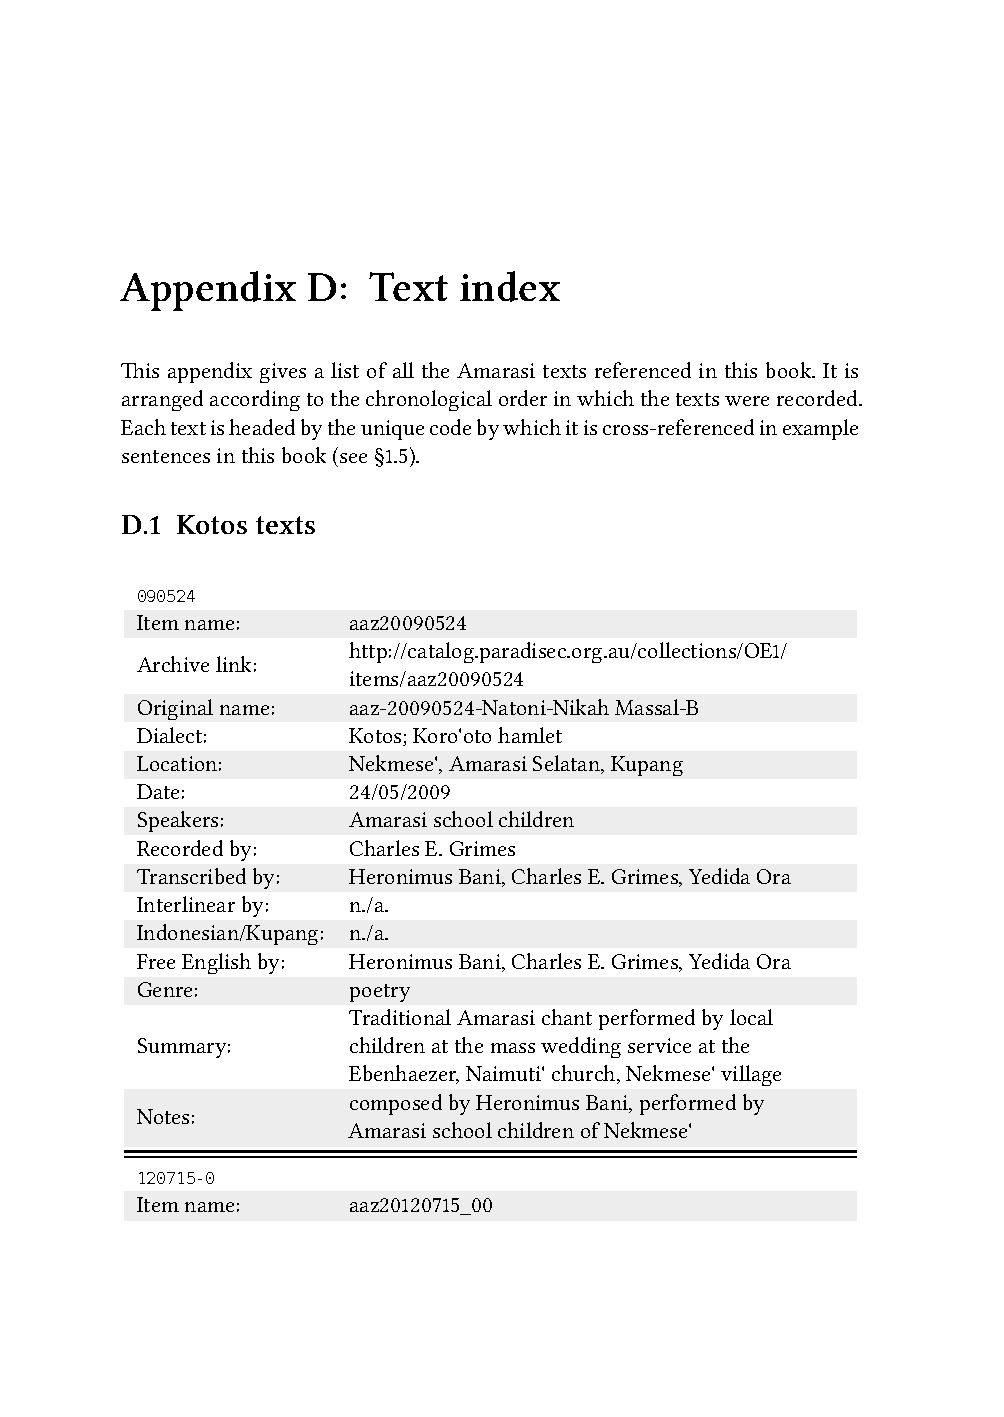
\includepdf[pages=-]{indexD.pdf}
% \chapter{Text index}\label{app:TexInd}
This appendix gives a list of all the texts referenced in this book.
It is arranged according to the chronological
order in which the texts were recorded.
Each text is headed by the unique code by which it is cross-referenced
in example sentences in this book (see \srf{sec:PreDat}).

\section{Kotos texts}

\noindent
\wg\begin{tabular}{lL{.67\textwidth}}
\xrf{090524}			& \\
Item name:			& aaz20090524\\
Archive link:			& \url{http://catalog.paradisec.org.au/collections/OE1/items/aaz20090524}\\
Original name:			& aaz-20090524-Natoni-Nikah Massal-B\\
Language:				& Amarasi [aaz] \\
Dialect:				& Kotos; Koro{\Q}oto hamlet \\
Location:				& Nekmese{\Q}, Amarasi Selatan, Kupang \\
Date:				& 24/05/2009\\
Speakers:				& Amarasi school children\\
Recorded by:			& Charles E. Grimes\\
Transcribed by:		& Heronimus Bani, Charles E. Grimes, Yedida Ora\\
Interlinear by:		& n./a.\\
Indonesian/Kupang:		& n./a.\\
Free English by:		& Heronimus Bani, Charles E. Grimes, Yedida Ora\\
Genre:				& poetry\\
Summary:				& Traditional Amarasi chant performed by local children at the mass wedding service at the Ebenhaezer, Naimuti{\Q} church, Nekmese{\Q} village\\
Length:				& \\
Notes:				& composed by Heronimus Bani, performed by Amarasi school children of Nekmese{\Q}\\
\end{tabular}

\newpage
\noindent
\wg\begin{tabular}{lL{.67\textwidth}}
\xrf{120715-0}			& \\
Item name:			& aaz20120715{\_}00\\
Archive link:			& \url{http://catalog.paradisec.org.au/collections/OE1/items/aaz20120715_00}\\
Original name:			& aaz-20120715-0-Nekmese-Natoni-2\\
Language:				& Amarasi [aaz] \\
Dialect:				& Kotos; Koro{\Q}oto hamlet \\
Location:				& Nekmese{\Q}, Amarasi Selatan, Kupang \\
Date:				& 24/05/2009\\
Speakers:				& Amarasi school children\\
Recorded by:			& Daniel Kaufman, Katharine Gosling\\
Transcribed by:		& Heronimus Bani, Charles E. Grimes, Yedida Ora\\
Interlinear by:		& n./a.\\
Indonesian/Kupang:		& n./a.\\
Free English by:		& Charles E. Grimes, Yedida Ora\\
Genre:				& poetry\\
Summary:				& Traditional Amarasi chant performed by local children of Koro{\Q}oto, Nekmese{\Q},
					to welcome Dan Kaufman and participants from the July 2015 Language Documentation Workshop\\
Length:				& \\
Notes:				& Composed by Heronimus Bani, performed by Amarasi school children of Nekmese{\Q} \\
video online:	&	\url{https://www.youtube.com/watch?v=TBqXhan5jl4& list=PLcXFPx-z7B0q_2Ns3iYHigEY77DG4kXSU& index=10}\\
\end{tabular}

\newpage
\noindent
\wg\begin{tabular}{lL{.67\textwidth}}
\xrf{120715-1}			& \\
Item name:			& aaz20120715{\_}01\\
Archive link:			& \url{http://catalog.paradisec.org.au/collections/OE1/items/aaz20120715_01}\\
Original name:			& aaz-20120715-1-Nekmese-Oma-1 \\
Language:				& Amarasi [aaz] \\
Dialect:				& Kotos; Fo{\Q}asa{\Q} hamlet \\
Location:				& Nekmese{\Q}, Amarasi Selatan, Kupang \\
Date:				& 15/07/2015 \\
Speakers:				& Yedida Ora \\
Recorded by:			& Daniel Kaufman, Katharine Gosling \\
Transcribed by:		& Yedida Ora \\
Interlinear by:		& Owen Edwards \\
Indonesian/Kupang:		& Yedida Ora \\
Free English by:		& Owen Edwards \\
Genre:				& narrative \\
Summary:				& Yedida Ora introduces herself and gives a short history of Nekmese{\Q} village \\
Length:				& 1.40 \\
Notes:				& \\
video online: & \url{https://www.youtube.com/watch?v=MwyNRkl1nBE& list=PLcXFPx-z7B0q_2Ns3iYHigEY77DG4kXSU& index=13} \\
\end{tabular}

\newpage
\noindent
\wg\begin{tabular}{lL{.67\textwidth}}
\xrf{120715-2}			& \\
Item name:			& aaz20120715{\_}02\\
Archive link:			& \url{http://catalog.paradisec.org.au/collections/OE1/items/aaz20120715_02}\\
Original name:			& aaz-20120715-2-Nekmese-Oma-2\\
Language:				& Amarasi [aaz] \\
Dialect:				& Kotos; Fo{\Q}asa{\Q} hamlet \\
Location:				& Nekmese{\Q}, Amarasi Selatan, Kupang \\
Date:				& 15/07/2015 \\
Speakers:				& Yedida Ora \\
Recorded by:			& Daniel Kaufman, Katharine Gosling \\
Transcribed by:		& Yedida Ora \\
Interlinear by:		& Owen Edwards \\
Indonesian/Kupang:		& Yedida Ora \\
Free English by:		& Owen Edwards \\
Genre:				& procedural \\
Summary:				& explanation about how the villagers of Nekmese{\Q} farm\\
Length:				& 1.39\\
Notes:				& video online \url{https://www.youtube.com/watch?v=NnjAlncqyV4& index=12& list=PLcXFPx-z7B0q_2Ns3iYHigEY77DG4kXSU}\\
\end{tabular}

\newpage
\noindent
\wg\begin{tabular}{lL{.67\textwidth}}
\xrf{120715-3}			& \\
Item name:			& aaz20120715{\_}03\\
Archive link:			& \url{http://catalog.paradisec.org.au/collections/OE1/items/aaz20120715_03}\\
Original name:			& aaz-20120715-3-Nekmese-KusnawiBani-1\\
Language:				& Amarasi [aaz] \\
Dialect:				& Kotos; Koro{\Q}oto hamlet \\
Location:				& Nekmese{\Q}, Amarasi Selatan, Kupang \\
Date:				& 15/07/2015 \\
Speakers:				& Taniel Feni, Kusnawi Bani\\
Recorded by:			& Daniel Kaufman, Heronimus Bani\\
Transcribed by:		& Yedida Ora\\
Interlinear by:		& Owen Edwards \\
Indonesian/Kupang:		& Yedida Ora\\
Free English by:		& Owen Edwards\\
Genre:				& folk-tale\\
Summary:				& a folk-tale about people who live on the moon\\
Length:				& 1.28\\
Notes:				& \\
video online: & \url{https://www.youtube.com/watch?v=H33aViriqy4& index=14& list=PLcXFPx-z7B0q_2Ns3iYHigEY77DG4kXSU}\\
\end{tabular}

\newpage
\noindent
\wg\begin{tabular}{lL{.67\textwidth}}
\xrf{120715-4}			& \\
Item name:			& \\
Archive link:			& \url{& /aaz20120715_04}\\
Original name:			& aaz-20120715-4-Nekmese-KusnawiBani-2\\
Language:				& Amarasi [aaz] \\
Dialect:				& Kotos; Koro{\Q}oto hamlet \\
Location:				& Nekmese{\Q}, Amarasi Selatan, Kupang \\
Date:				& 15/07/2015 \\
Speakers:				& Taniel Feni, Kusnawi Bani, (Heronimus Bani)\\
Recorded by:			& Daniel Kaufman, Heronimus Bani\\
Transcribed by:		& Yedida Ora\\
Interlinear by:		& Owen Edwards \\
Indonesian/Kupang:		& Yedida Ora\\
Free English by:		& Owen Edwards\\
Genre:				& folk-tales\\
Summary:				& a series of folk-tales: \\
					& 1. Moo{\Q}-hitu: a mythical snake who created the world (0.00--3.03)\\
					& 2. Brao stones: explanation of the source of a landscape feature (3.03--4.23)\\
					& 3. Nii Obe{\Q}: the king of Koro{\Q}oto (4.26--5.19)\\
					& 4. How the village of Koro{\Q}oto got its name (5.27--6.30)\\
					& 6. How the village of Ansaof got its name  (6.34--7.33)\\
					& 7. How the village of Kiu Mabanat got its name (7.35--8.11)\\
Length:				& 8.33\\
Notes:				&\\
video online: &\url{https://www.youtube.com/watch?v=Z_2D9WhYuuM& list=PLcXFPx-z7B0q_2Ns3iYHigEY77DG4kXSU& index=15}\\
\end{tabular}

\newpage
\noindent
\wg\begin{tabular}{lL{.67\textwidth}}
\xrf{120923-1}			& \\
Item name:			& aaz20120923{\_}01\\
Archive link:			& \url{http://catalog.paradisec.org.au/collections/OE1/items/aaz20120923_01}\\
Original name:			& aaz-20120923-1-MelkiasMnao-Nekmese-biku\\
Language:				& Amarasi [aaz] \\
Dialect:				& Kotos; Koro{\Q}oto hamlet \\
Location:				& Nekmese{\Q}, Amarasi Selatan, Kupang \\
Date:				& 23/09/2012\\
Speakers:				& Melkias Mna{\Q}o, (Heronimus Bani)\\
Recorded by:			& Heronimus Bani\\
Transcribed by:		& Heronimus Bani\\
Interlinear by:		& Owen Edwards \\
Indonesian/Kupang:		& n./a.\\
Free English by:		& Owen Edwards\\
Genre:				& narrative\\
Summary:				& Melkias tells Roni about a time someone cast the \it{biku} curse.
						He does so to discourage others from doing likewise.
						He also partially explains the method by which it is cast after Roni asks. \\
Length:				& 13.14\\
Notes:				& Melkias Mna{\Q}o has lived in Binoni-Aufme{\Q}e hamlet (village Oenoni 2) for quite some time\\
\end{tabular}

\newpage
\noindent
\wg\begin{tabular}{lL{.67\textwidth}}
\xrf{120923-2}			& \\
Item name:			& \\
Archive link:			& \url{& /aaz20120923_02}\\
Original name:			& aaz-20120923-2-MelkiasMnao-Nekmese-bunu\\
Language:				& Amarasi [aaz] \\
Dialect:				& Kotos; Koro{\Q}oto hamlet \\
Location:				& Nekmese{\Q}, Amarasi Selatan, Kupang \\
Date:				& 23/09/2012\\
Speakers:				& Melkias Mna{\Q}o, (Heronimus Bani)\\
Recorded by:			& Heronimus Bani\\
Transcribed by:		& Heronimus Bani\\
Interlinear by:		& Owen Edwards \\
Indonesian/Kupang:		& Heronimus Bani\\
Free English by:		& Owen Edwards \\
Genre:				& procedural\\
Summary:				& Melkias Mna{\Q}o explains how one can use \it{bunu}
						to protect their crops from being stolen\\
Length:				& 7.05\\
Notes:				& Melkias Mna{\Q}o has lived in Binoni-Aufme{\Q}e hamlet (village Oenoni 2) for quite some time\\
\end{tabular}

\newpage
\noindent
\wg\begin{tabular}{lL{.67\textwidth}}
\xrf{130821-1}			& \\
Item name:			& aaz20130821{\_}01\\
Archive link:			& \url{http://catalog.paradisec.org.au/collections/OE1/items/aaz20130821_01}\\
Original name:			& aaz-20130821-1-Nekmese-Funeral\\
Language:				& Amarasi [aaz] \\
Dialect:				& Kotos; Koro{\Q}oto hamlet \\
Location:				& Nekmese{\Q}, Amarasi Selatan, Kupang \\
Date:				& 21/08/2013\\
Speakers:				& Heronimus Bani\\
Recorded by:			& Owen Edwards\\
Transcribed by:		& Heronimus Bani\\
Interlinear by:		& Owen Edwards \\
Indonesian/Kupang:		& Heronimus Bani\\
Free English by:		& Owen Edwards\\
Genre:				& narrative\\
Summary:				& 1. Heronimus Bani explains to an audience that Owen Edwards
						has come to stay in Nekmese{\Q} village to learn Amarasi\\
					& 2. Heronimus Bani gives the genealogy of his recently deceased maternal aunt, Sarlina\\
Length:				& 10.10\\
Notes:				& \\
\end{tabular}

\newpage
\noindent
\wg\begin{tabular}{lL{.67\textwidth}}
\xrf{130822-1}			& \\
Item name:			& aaz20130822{\_}01\\
Archive link:			& \url{http://catalog.paradisec.org.au/collections/OE1/items/aaz20130822_01}\\
Original name:			& aaz-20130822-1-HeronimusBani-Kuareno\\
Language:				& Amarasi [aaz] \\
Dialect:				& Kotos; Koro{\Q}oto hamlet \\
Location:				& Nekmese{\Q}, Amarasi Selatan, Kupang \\
Date:				& 22/08/2013\\
Speakers:				& Heronimus Bani\\
Recorded by:			& Owen Edwards\\
Transcribed by:		& Yedida Ora\\
Interlinear by:		& Owen Edwards \\
Indonesian/Kupang:		& n./a.\\
Free English by:		& Owen Edwards\\
Genre:				& narrtive\\
Summary:				& explanation of how the village Kuareno{\Q} got its name\\
Length:				& 0.41\\
Notes:				& \\
\end{tabular}

\newpage
\noindent
\wg\begin{tabular}{lL{.67\textwidth}}
\xrf{130823-2}			& \\
Item name:			& aaz20130823{\_}02\\
Archive link:			& \url{http://catalog.paradisec.org.au/collections/OE1/items/aaz20130823_02}\\
Original name:			& aaz-20130823-2-YurmemisOra-Kuareno\\
Language:				& Amarasi [aaz] \\
Dialect:				& Kotos; Koro{\Q}oto hamlet \\
Location:				& Nekmese{\Q}, Amarasi Selatan, Kupang \\
Date:				& 23/08/2013\\
Speakers:				& Yurmemis Ora\\
Recorded by:			& Owen Edwards\\
Transcribed by:		& Yedida Ora, Heronimus Bani\\
Interlinear by:		& Owen Edwards \\
Indonesian/Kupang:		& Heronimus Bani\\
Free English by:		& Owen Edwards\\
Genre:				& narrative \\
Summary:				& explanation of how the village Kuareno{\Q} got its name\\
Length:				& 1.15\\
Notes:				& \\
\end{tabular}

\newpage
\noindent
\wg\begin{tabular}{lL{.67\textwidth}}
\xrf{130823-5}			& \\
Item name:			& aaz20130823{\_}05\\
Archive link:			& \url{http://catalog.paradisec.org.au/collections/OE1/items/aaz20130823_05}\\
Original name:			& aaz-20130823-5-EliotNubatonis\\
Language:				& Amarasi [aaz] \\
Dialect:				& Kotos; Koro{\Q}oto hamlet \\
Location:				& Nekmese{\Q}, Amarasi Selatan, Kupang \\
Date:				& 23/08/2013\\
Speakers:				& Eliot Nubatonis\\
Recorded by:			& Owen Edwards\\
Transcribed by:		& Yedida Ora\\
Interlinear by:		& Owen Edwards \\
Indonesian/Kupang:		& n./a.\\
Free English by:		& Owen Edwards\\
Genre:				& auction\\
Summary:				& an auction of some rice and pork\\
Length:				& 1.23\\
Notes:				& \\
\end{tabular}

\newpage
\noindent
\wg\begin{tabular}{lL{.67\textwidth}}
\xrf{130823-8}			& \\
Item name:			& aaz20130823{\_}08\\
Archive link:			& \url{http://catalog.paradisec.org.au/collections/OE1/items/aaz20130823_08}\\
Original name:			& aaz-20130823-8-menangis\\
Language:				& Amarasi [aaz] \\
Dialect:				& Kotos; Naet hamlet \\
Location:				& Nekmese{\Q}, Amarasi Selatan, Kupang \\
Date:				& 23/08/2013\\
Speakers:				& \\
Recorded by:			& Owen Edwards\\
Transcribed by:		& Yedida Ora\\
Interlinear by:		& Owen Edwards \\
Indonesian/Kupang:		& Heronimus Bani\\
Free English by:		& Owen Edwards\\
Genre:				& mourning\\
Summary:				& a woman mourns for her recently deceased grandmother\\
Length:				& 9.45\\
Notes:				& \\
\end{tabular}

\newpage
\noindent
\wg\begin{tabular}{lL{.67\textwidth}}
\xrf{130823-9}			& \\
Item name:			& aaz20130823{\_}09\\
Archive link:			& \url{http://catalog.paradisec.org.au/collections/OE1/items/aaz20130823_09}\\
Original name:			& aaz-20130823-9-GersonNee\\
Language:				& Amarasi [aaz] \\
Dialect:				& Kotos; Koro{\Q}oto hamlet \\
Location:				& Nekmese{\Q}, Amarasi Selatan, Kupang \\
Date:				& 23/08/2013\\
Speakers:				& Gerson Nee\\
Recorded by:			& Owen Edwards\\
Transcribed by:		& Yedida Ora\\
Interlinear by:		& Owen Edwards \\
Indonesian/Kupang:		& Heronimus Bani\\
Free English by:		& Owen Edwards\\
Genre:				& narrative\\
Summary:				& how the hamlet of Naet got its name\\
Length:				& 0.43\\
Notes:				& \\
\end{tabular}

\newpage
\noindent
\wg\begin{tabular}{lL{.67\textwidth}}
\xrf{130825-3}			& \\
Item name:			& aaz20130825{\_}03\\
Archive link:			& \url{http://catalog.paradisec.org.au/collections/OE1/items/aaz20130825_03}\\
Original name:			& aaz-20130825-3-LukasOra-Nekmese\\
Language:				& Amarasi [aaz] \\
Dialect:				& Kotos; Koro{\Q}oto hamlet \\
Location:				& Nekmese{\Q}, Amarasi Selatan, Kupang \\
Date:				& 25/08/2013\\
Speakers:				& Lukas Ora\\
Recorded by:			& Heronimus Bani\\
Transcribed by:		& Heronimus Bani\\
Interlinear by:		& Owen Edwards \\
Indonesian/Kupang:		& Heronimus Bani\\
Free English by:		& Owen Edwards\\
Genre:				& poetry\\
Summary:				& greeting for new government officials\\
Length:				& 2.54\\
Notes:				& high wind and feedback from the loudspeaker reduce recording quality\\
\end{tabular}

\newpage
\noindent
\wg\begin{tabular}{lL{.67\textwidth}}
\xrf{130825-6}			& \\
Item name:			& aaz20130825{\_}06\\
Archive link:			& \url{http://catalog.paradisec.org.au/collections/OE1/items/aaz20130825_06}\\
Original name:			& aaz-20130825-6-JonathanNamah-1\\
Language:				& Amarasi [aaz] \\
Dialect:				& Kotos; Koro{\Q}oto hamlet \\
Location:				& Nekmese{\Q}, Amarasi Selatan, Kupang \\
Date:				& 25/08/2013\\
Speakers:				& Jonathan Namah, Heronimus Bani, several others interrupt \\
Recorded by:			& Heronimus Bani\\
Transcribed by:		& Heronimus Bani\\
Interlinear by:		& Owen Edwards \\
Indonesian/Kupang:		& Heronimus Bani\\
Free English by:		& Owen Edwards (only first seven minutes)\\
Genre:				& narrative, (conversation)\\
Summary:				& 1. story about Church (0.00-5.46)\\
					& 2. story about the time Jonathan went to Jakarta,
						up until the time he was on the plane from Kupang\\
Length:				& 23.10\\
Notes:				& continued as \xrf{130825-7} (see below) \\
					& loud background music and people often interrupt/talk over Jonathan.
						Roni did a \it{fantastic} job transcribing this! \\
\end{tabular}

\newpage
\noindent
\wg\begin{tabular}{lL{.67\textwidth}}
\xrf{130825-7}			& \\
Item name:			& aaz20130825{\_}07\\
Archive link:			& \url{http://catalog.paradisec.org.au/collections/OE1/items/aaz20130825_07}\\
Original name:			& aaz-20130825-7-JonathanNamah-2\\
Language:				& Amarasi [aaz] \\
Dialect:				& Kotos; Koro{\Q}oto hamlet \\
Location:				& Nekmese{\Q}, Amarasi Selatan, Kupang \\
Date:				& 25/08/2013\\
Speakers:				& Jonathan Namah, Heronimus Bani, several others interrupt \\
Recorded by:			& Heronimus Bani\\
Transcribed by:		& Heronimus Bani\\
Interlinear by:		& Owen Edwards \\
Indonesian/Kupang:		& Heronimus Bani\\
Free English by:		& n./a.\\
Genre:				& narrative\\
Summary:				& Jonathan relates his experience in the hotel in Jakarta\\
Length:				& 4.01\\
Notes:				& continuation of \xrf{130825-6} above, \\
					& loud background music and people often interrupt/talk over Jonathan. \\
\end{tabular}

\newpage
\noindent
\wg\begin{tabular}{lL{.67\textwidth}}
\xrf{130825-8}			& \\
Item name:			& aaz20130825{\_}08\\
Archive link:			& \url{http://catalog.paradisec.org.au/collections/OE1/items/aaz20130825_08}\\
Original name:			& aaz-20130825-8-JonathanNamah-3\\
Language:				& Amarasi [aaz] \\
Dialect:				& Kotos; Koro{\Q}oto hamlet \\
Location:				& Nekmese{\Q}, Amarasi Selatan, Kupang \\
Date:				& 25/08/2013\\
Speakers:				& Jonathan Namah, Heronimus Bani, several others interrupt \\
Recorded by:			& Heronimus Bani\\
Transcribed by:		& Heronimus Bani\\
Interlinear by:		& Owen Edwards \\
Indonesian/Kupang:		& Heronimus Bani\\
Free English by:		& n./a.\\
Genre:				& narrative\\
Summary:				& Jonathan relates his experience in the hotel in Jakarta\\
Length:				& 2.20\\
Notes:				& continuation of \xrf{130825-7} above, \\
					& loud background music and people often interrupt/talk over Jonathan. \\
\end{tabular}

\newpage
\noindent
\wg\begin{tabular}{lL{.67\textwidth}}
\xrf{130902-1}			& \\
Item name:			& aaz20130902{\_}01\\
Archive link:			& \url{http://catalog.paradisec.org.au/collections/OE1/items/aaz20130902_01}\\
Original name:			& aaz-20130902-1-HeronimusBani-Cerita-JumatSenin\\
Language:				& Amarasi [aaz] \\
Dialect:				& Kotos; Koro{\Q}oto hamlet \\
Location:				& Nekmese{\Q}, Amarasi Selatan, Kupang \\
Date:				& 02/09/2013\\
Speakers:				& Heronimus Bani\\
Recorded by:			& Heronimus Bani\\
Transcribed by:		& Heronimus Bani\\
Interlinear by:		& Owen Edwards \\
Indonesian/Kupang:		& Heronimus Bani\\
Free English by:		& n./a.\\
Genre:				& narrative\\
Summary:				& Heronimus Bani relates the things he and Owen Edwards did over the past few days\\
Length:				& 4.38\\
Notes:				& \\
\end{tabular}

\newpage
\noindent
\wg\begin{tabular}{lL{.67\textwidth}}
\xrf{130902-7}			& \\
Item name:			& aaz20130902{\_}07\\
Archive link:			& \url{http://catalog.paradisec.org.au/collections/OE1/items/aaz20130902_07}\\
Original name:			& {\small aaz-20130902-7-HeronimusBani-IsakFeni-BahasaAdat}\\
Language:				& Amarasi [aaz] \\
Dialect:				& Kotos; Koro{\Q}to hamlet, Ro{\Q}is; Buraen village \\
Location:				& Nekmese{\Q}, Amarasi Selatan, Kupang \\
Date:				& 02/09/2013\\
Speakers:				& Heronimus Bani (Kotos), Isak Feni (Ro{\Q}is)\\
Recorded by:			& Heronimus Bani\\
Transcribed by:		& Heronimus Bani\\
Interlinear by:		& Owen Edwards \\
Indonesian/Kupang:		& Heronimus Bani\\
Free English by:		& n./a.\\
Genre:				& ritual speech \\
Summary:				& formal conversation about marriage arrangements\\
Length:				& 5.50\\
Notes:				& \\
\end{tabular}

\newpage
\noindent
\wg\begin{tabular}{lL{.67\textwidth}}
\xrf{130905-1}			& \\
Item name:			& aaz20130905{\_}01\\
Archive link:			& \url{http://catalog.paradisec.org.au/collections/OE1/items/aaz20130905_01}\\
Original name:			& {\footnotesize aaz-20130905-1-HeronimusBani-arahan-pilkada-bupati-kupang}\\
Language:				& Amarasi [aaz] \\
Dialect:				& Kotos; Koro{\Q}oto hamlet \\
Location:				& Nekmese{\Q}, Amarasi Selatan, Kupang \\
Date:				& 05/09/2013\\
Speakers:				& Heronimus Bani\\
Recorded by:			& Owen Edwards\\
Transcribed by:		& Heronimus Bani\\
Interlinear by:		& Owen Edwards \\
Indonesian/Kupang:		& Heronimus Bani\\
Free English by:		& n./a.\\
Genre:				& procedural\\
Summary:				& Heronimus Bani gives instructions on how to vote for the Kupang bupati (regent)\\
Length:				& 1.47\\
Notes:				& recording starts part way through, entirety videoed \\
\end{tabular}

\newpage
\noindent
\wg\begin{tabular}{lL{.67\textwidth}}
\xrf{130906-1}			& \\
Item name:			& aaz20130906{\_}01\\
Archive link:			& \url{http://catalog.paradisec.org.au/collections/OE1/items/aaz20130906_01}\\
Original name:			& aaz-20130906-1-JakopBani-percakapan\\
Language:				& Amarasi [aaz] \\
Dialect:				& Kotos; Koro{\Q}oto hamlet \\
Location:				& Nekmese{\Q}, Amarasi Selatan, Kupang \\
Date:				& 06/09/2013\\
Speakers:				& Jakop Bani, Heronimus Bani, (Lena Bani)\\
Recorded by:			& Heronimus Bani\\
Transcribed by:		& Heronimus Bani\\
Interlinear by:		& Owen Edwards \\
Indonesian/Kupang:		& Heronimus Bani\\
Free English by:		& n./a.\\
Genre:				& conversation\\
Summary:				& \\
Length:				& 6.11\\
Notes:				& \\
\end{tabular}

\newpage
\noindent
\wg\begin{tabular}{lL{.67\textwidth}}
\xrf{130907-3}			& \\
Item name:			& aaz20130907{\_}03\\
Archive link:			& \url{http://catalog.paradisec.org.au/collections/OE1/items/aaz20130907_03}\\
Original name:			& aaz-20130907-3-FransBani-Cerita-1\\
Language:				& Amarasi [aaz] \\
Dialect:				& Kotos; Koro{\Q}oto hamlet \\
Location:				& Nekmese{\Q}, Amarasi Selatan, Kupang \\
Date:				& 07/09/2013\\
Speakers:				& Frans Bani\\
Recorded by:			& Heronimus Bani\\
Transcribed by:		& Heronimus Bani\\
Interlinear by:		& Owen Edwards Heronimus Bani\\
Indonesian/Kupang:		& Heronimus Bani\\
Free English by:		& n./a.\\
Genre:				& narrative\\
Summary:				& Frans Bani (Roni's dad) tells his life story from the time he was at school up until the birth of his first child\\
Length:				& 15.37\\
Notes:				& faint recording, people sifting rice loudly in background\\
\end{tabular}

\newpage
\noindent
\wg\begin{tabular}{lL{.67\textwidth}}
\xrf{130907-4}			& \\
Item name:			& aaz20130907{\_}04 \\
Archive link:			& \url{http://catalog.paradisec.org.au/collections/OE1/items/aaz20130907_04 }\\
Original name:			& aaz-20130907-4-FransBani-Cerita-2\\
Language:				& Amarasi [aaz] \\
Dialect:				& Kotos; Koro{\Q}oto hamlet \\
Location:				& Nekmese{\Q}, Amarasi Selatan, Kupang \\
Date:				& 07/09/2013\\
Speakers:				& Frans Bani\\
Recorded by:			& Heronimus Bani\\
Transcribed by:		& Heronimus Bani\\
Interlinear by:		& Owen Edwards Heronimus Bani\\
Indonesian/Kupang:		& Heronimus Bani\\
Free English by:		& n./a.\\
Genre:				& narrative\\
Summary:				& Frans Bani talks about his children's schooling\\
Length:				& 4.07\\
Notes:				& faint recording, people sifting rice loudly in background\\
\end{tabular}

\newpage
\noindent
\wg\begin{tabular}{lL{.67\textwidth}}
\xrf{130907-4}			& \\
Item name:			& aaz20130907{\_}05\\
Archive link:			& \url{http://catalog.paradisec.org.au/collections/OE1/items/aaz20130907_05}\\
Original name:			& aaz-20130907-5-FransBani-Cerita-3\\
Language:				& Amarasi [aaz] \\
Dialect:				& Kotos; Koro{\Q}oto hamlet \\
Location:				& Nekmese{\Q}, Amarasi Selatan, Kupang \\
Date:				& 07/09/2013\\
Speakers:				& Frans Bani\\
Recorded by:			& Heronimus Bani\\
Transcribed by:		& Heronimus Bani\\
Interlinear by:		& Owen Edwards Heronimus Bani\\
Indonesian/Kupang:		& Heronimus Bani\\
Free English by:		& n./a.\\
Genre:				& narrative\\
Summary:				& Frans Bani talks about working for the Church\\
Length:				& 2.04\\
Notes:				& faint recording, people sifting rice loudly in background\\
\end{tabular}

\newpage
\noindent
\wg\begin{tabular}{lL{.67\textwidth}}
\xrf{130909-5}			& \\
Item name:			& aaz20130909{\_}05\\
Archive link:			& \url{http://catalog.paradisec.org.au/collections/OE1/items/aaz20130909_05}\\
Original name:			& aaz-20130909-5-AlfonsusTakain-OmongMasala-3\\
Language:				& Amarasi [aaz] \\
Dialect:				& Kotos; Koro{\Q}oto hamlet \\
Location:				& Nekmese{\Q}, Amarasi Selatan, Kupang \\
Date:				& 09/09/2015\\
Speakers:				& Alfonsus Takain\\
Recorded by:			& Heronimus Bani\\
Transcribed by:		& Heronimus Bani\\
Interlinear by:		& Owen Edwards \\
Indonesian/Kupang:		& Heronimus Bani\\
Free English by:		& n./a.\\
Genre:				& narrative\\
Summary:				& Alfonsus relates a mistake made in the counting and collection of Church offertories\\
Length:				& 1.10\\
Notes:				& \\
\end{tabular}

\newpage
\noindent
\wg\begin{tabular}{lL{.67\textwidth}}
\xrf{130909-6}			& \\
Item name:			& aaz20130909{\_}06\\
Archive link:			& \url{http://catalog.paradisec.org.au/collections/OE1/items/aaz20130909_06}\\
Original name:			& aaz-20130909-6-ObetBani-CeritaKeluargaDiRumah\\
Language:				& Amarasi [aaz] \\
Dialect:				& Kotos; Koro{\Q}oto hamlet \\
Location:				& Nekmese{\Q}, Amarasi Selatan, Kupang \\
Date:				& 09/09/2013\\
Speakers:				& Heronimus Bani, Obet Bani, Ema Bani, \\
Recorded by:			& Heronimus Bani\\
Transcribed by:		& Heronimus Bani\\
Interlinear by:		& Owen Edwards \\
Indonesian/Kupang:		& Heronimus Bani\\
Free English by:		& n./a.\\
Genre:				& conversation\\
Summary:				& conversation about Obet's life at home without his children (who are working elsewhere)\\
Length:				& 4.14\\
Notes:				& \\
\end{tabular}

\newpage
\noindent
\wg\begin{tabular}{lL{.67\textwidth}}
\xrf{130911-2}			& \\
Item name:			& aaz20130911{\_}02\\
Archive link:			& \url{http://catalog.paradisec.org.au/collections/OE1/items/aaz20130911_02}\\
Original name:			& {\small aaz-20130911-2-DominggusBani-HenkiOra-CeritaOtoJato}\\
Language:				& Amarasi [aaz] \\
Dialect:				& Kotos; Koro{\Q}oto hamlet \\
Location:				& Nekmese{\Q}, Amarasi Selatan, Kupang \\
Date:				& 11/09/2013\\
Speakers:				& Dominggus Bani, Heronimus Bani, Sefnat Bois, Henki Ora, occasional others\\
Recorded by:			& Heronimus Bani\\
Transcribed by:		& Heronimus Bani\\
Interlinear by:		& Owen Edwards \\
Indonesian/Kupang:		& Heronimus Bani\\
Free English by:		& Owen Edwards\\
Genre:				& conversation\\
Summary:				& conversation about a car which crashed and came off the road\\
Length:				& 1.43\\
Notes:				& \\
\end{tabular}

\newpage
\noindent
\wg\begin{tabular}{lL{.67\textwidth}}
\xrf{130912}			& \\
Item name:			& aaz20130912\\
Archive link:			& \url{http://catalog.paradisec.org.au/collections/OE1/items/aaz20130912}\\
Original name:			& {\footnotesize aaz-20130912-HeronimusBani-cerita-pulang-dari-orang-mati}\\
Language:				& Amarasi [aaz] \\
Dialect:				& Kotos; Koro{\Q}oto hamlet \\
Location:				& Nekmese{\Q}, Amarasi Selatan, Kupang \\
Date:				& 12/09/2013\\
Speakers:				& Heronimus Bani, Rehuel Nakmofa, Sem Saebesi\\
Recorded by:			& Heronimus Bani\\
Transcribed by:		& Heronimus Bani\\
Interlinear by:		& Owen Edwards \\
Indonesian/Kupang:		& Heronimus Bani\\
Free English by:		& n./a.\\
Genre:				& conversation\\
Summary:				& conversation about someone who recently died\\
Length:				& 1.01\\
Notes:				& \\
\end{tabular}

\newpage
\noindent
\wg\begin{tabular}{lL{.67\textwidth}}
\xrf{130913-1}			& \\
Item name:			& aaz20130913{\_}01\\
Archive link:			& \url{http://catalog.paradisec.org.au/collections/OE1/items/aaz20130913_01}\\
Original name:			& aaz-20130913-1-ItkaNenoharan-MerpatiTakain-Cerita\\
Language:				& Amarasi [aaz] \\
Dialect:				& Kotos; Koro{\Q}oto hamlet, Fo{\Q}asa{\Q} hamlet \\
Location:				& Nekmese{\Q}, Amarasi Selatan, Kupang \\
Date:				& 13/09/2013\\
Speakers:				& Heronimus Bani, Itka Nenoharan, Merpati Takain, Justus Mantolas\\
Recorded by:			& Heronimus Bani\\
Transcribed by:		& Heronimus Bani\\
Interlinear by:		& Owen Edwards \\
Indonesian/Kupang:		& Heronimus Bani\\
Free English by:		& n./a.\\
Genre:				& conversation\\
Summary:				& a conversation about a man who has already made preparations for his funeral,
						even though he's still fit and healthy\\
Length:				& 3.03\\
Notes:				& Itka Nenoharan is from Fo{\Q}asa{\Q},
						Justus Mantolas is originally from Amanatun.
						(Hence, the phoneme /l/.)
						He has lived in Nekmese{\Q} since 1981.\\
\end{tabular}

\newpage
\noindent
\wg\begin{tabular}{lL{.67\textwidth}}
\xrf{130914-1}			& \\
Item name:			& aaz20130914{\_}01\\
Archive link:			& \url{http://catalog.paradisec.org.au/collections/OE1/items/aaz20130914_01}\\
Original name:			& aaz-20130914-1-MateldaBani-cerita-kerja-tenun\\
Language:				& Amarasi [aaz] \\
Dialect:				& Kotos; Koro{\Q}oto hamlet \\
Location:				& Nekmese{\Q}, Amarasi Selatan, Kupang \\
Date:				& 14/09/2013\\
Speakers:				& Metelda Bani, Heronimus Bani\\
Recorded by:			& Heronimus Bani\\
Transcribed by:		& Heronimus Bani\\
Interlinear by:		& Owen Edwards \\
Indonesian/Kupang:		& Heronimus Bani\\
Free English by:		& n./a.\\
Genre:				& conversation\\
Summary:				& conversation about how to weave\\
Length:				& 3.03\\
Notes:				& \\
\end{tabular}

\newpage
\noindent
\wg\begin{tabular}{lL{.67\textwidth}}
\xrf{130914-2}			& \\
Item name:			& aaz20130914{\_}02\\
Archive link:			& \url{http://catalog.paradisec.org.au/collections/OE1/items/aaz20130914_02}\\
Original name:			& {\footnotesize aaz-20130914-2-Regina-Sarai-Sarmolina-cerita-ternak-lepas}\\
Language:				& Amarasi [aaz] \\
Dialect:				& Kotos; Koro{\Q}oto hamlet, Fo{\Q}asa{\Q} hamlet \\
Location:				& Nekmese{\Q}, Amarasi Selatan, Kupang \\
Date:				& 14/09/2016\\
Speakers:				& Regina, Sarai, Sarmolina\\
Recorded by:			& Heronimus Bani\\
Transcribed by:		& Heronimus Bani\\
Interlinear by:		& Owen Edwards \\
Indonesian/Kupang:		& Heronimus Bani\\
Free English by:		& n./a.\\
Genre:				& conversation\\
Summary:				& conversation about some pigs which escaped\\
Length:				& 1.36\\
Notes:				& Regina is from Fo{\Q}asa{\Q} hamlet\\
\end{tabular}

\newpage
\noindent
\wg\begin{tabular}{lL{.67\textwidth}}
\xrf{130914-3}			& \\
Item name:			& aaz20130914{\_}03\\
Archive link:			& \url{http://catalog.paradisec.org.au/collections/OE1/items/aaz20130914_03}\\
Original name:			& {\small aaz-20130914-3-Sarmolina-Lena-cerita-jalan-pi-Sonraen}\\
Language:				& Amarasi [aaz] \\
Dialect:				& Kotos; Koro{\Q}oto hamlet \\
Location:				& Nekmese{\Q}, Amarasi Selatan, Kupang \\
Date:				& 14/09/2013\\
Speakers:				& Sarmolina, Lena Bani, Regina\\
Recorded by:			& Heronimus Bani\\
Transcribed by:		& Heronimus Bani\\
Interlinear by:		& Owen Edwards \\
Indonesian/Kupang:		& Heronimus Bani\\
Free English by:		& n./a.\\
Genre:				& conversation\\
Summary:				& conversation about when Sarmolina went to Sonraen\\
Length:				& 2.21\\
Notes:				& \\
\end{tabular}

\newpage
\noindent
\wg\begin{tabular}{lL{.67\textwidth}}
\xrf{130920-1}			& \\
Item name:			& aaz20130920{\_}01\\
Archive link:			& \url{http://catalog.paradisec.org.au/collections/OE1/items/aaz20130920_01}\\
Original name:			& {\small aaz-20130920-1-HeronimusBani-CeritaTtgFinalCheck}\\
Language:				& Amarasi [aaz] \\
Dialect:				& Kotos; Koro{\Q}oto hamlet \\
Location:				& Kupang city\\
Date:				& 20/09/2013\\
Speakers:				& Heronimus Bani\\
Recorded by:			& Owen Edwards\\
Transcribed by:		& Heronimus Bani\\
Interlinear by:		& Owen Edwards \\
Indonesian/Kupang:		& Heronimus Bani\\
Free English by:		& n./a.\\
Genre:				& narrative\\
Summary:				& Roni talks about his work over the past week proofreading books
						of the Bible and cheking them for naturalness
						with a group of villagers from Nekmese{\Q}\\
Length:				& 5.17\\
Notes:				& recorded in studio to get a high quality recording\\
\end{tabular}

\newpage
\noindent
\wg\begin{tabular}{lL{.67\textwidth}}
\xrf{130921-1}			& \\
Item name:			& aaz20130921{\_}01\\
Archive link:			& \url{http://catalog.paradisec.org.au/collections/OE1/items/aaz20130921_01}\\
Original name:			& aaz-20130921-1-YedidaOra-CeritaTtgFinalCheck\\
Language:				& Amarasi [aaz] \\
Dialect:				& Kotos; Fo{\Q}asa{\Q} hamlet \\
Location:				& Kupang city\\
Date:				& 21/09/2013\\
Speakers:				& Yedida Ora\\
Recorded by:			& Owen Edwards\\
Transcribed by:		& Yedida Ora\\
Interlinear by:		& Owen Edwards \\
Indonesian/Kupang:		& n./a.\\
Free English by:		& Owen Edwards\\
Genre:				& narrative\\
Summary:				& Oma talks about her work over the past week proofreading books
						of the Bible and cheking them for naturalness
						with a group of villagers from Nekmese{\Q}\\
Length:				& 2.17\\
Notes:				& recorded in studio to get a high quality recording\\
\end{tabular}

\newpage
\noindent
\wg\begin{tabular}{lL{.67\textwidth}}
\xrf{130925-1}			& \\
Item name:			& aaz20130925{\_}01\\
Archive link:			& \url{http://catalog.paradisec.org.au/collections/OE1/items/aaz20130925_01}\\
Original name:			& aaz-20130925-1-AlbertBani-etal-PencurianSapi\\
Language:				& Amarasi [aaz] \\
Dialect:				& Kotos; Koro{\Q}oto hamlet \\
Location:				& Nekmese{\Q}, Amarasi Selatan, Kupang \\
Date:				& 25/09/2013\\
Speakers:				& Albert Bani, Metheos Ora, Alfrid Bani, Heronimus Bani\\
Recorded by:			& Heronimus Bani\\
Transcribed by:		& Heronimus Bani\\
Interlinear by:		& Owen Edwards \\
Indonesian/Kupang:		& Heronimus Bani\\
Free English by:		& n./a.\\
Genre:				& conversation\\
Summary:				& conversation about someone who was stealing cows\\
Length:				& 4.50\\
Notes:				& \\
\end{tabular}

\newpage
\noindent
\wg\begin{tabular}{lL{.67\textwidth}}
\xrf{130926-1}			& \\
Item name:			& aaz20130926{\_}01\\
Archive link:			& \url{http://catalog.paradisec.org.au/collections/OE1/items/aaz20130926_01}\\
Original name:			& aaz-20130926-1-RidolfNeno-OmongIisBelis\\
Language:				& Amarasi [aaz] \\
Dialect:				& Kotos; Koro{\Q}oto hamlet \\
Location:				& Nekmese{\Q}, Amarasi Selatan, Kupang \\
Date:				& 26/09/2013\\
Speakers:				& Ridolf Neno, Heronimus Bani\\
Recorded by:			& Heronimus Bani\\
Transcribed by:		& Heronimus Bani\\
Interlinear by:		& Owen Edwards \\
Indonesian/Kupang:		& Heronimus Bani\\
Free English by:		& n./a.\\
Genre:				& conversation\\
Summary:				& Roni and Ridolf discuss bride-price arrangements\\
Length:				& 4.20\\
Notes:				& final half minute not transcribed\\
\end{tabular}

\newpage
\noindent
\wg\begin{tabular}{lL{.67\textwidth}}
\xrf{130928-1}			& \\
Item name:			& aaz20130928{\_}01\\
Archive link:			& \url{http://catalog.paradisec.org.au/collections/OE1/items/aaz20130928_01}\\
Original name:			& {\small aaz-20130928-1-HeronimusBani-CeritaNahorBaniMati}\\
Language:				& Amarasi [aaz] \\
Dialect:				& Kotos; Koro{\Q}oto hamlet \\
Location:				& Nekmese{\Q}, Amarasi Selatan, Kupang \\
Date:				& 28/09/2013\\
Speakers:				& Heronimus Bani\\
Recorded by:			& Heronimus Bani\\
Transcribed by:		& Heronimus Bani\\
Interlinear by:		& Owen Edwards \\
Indonesian/Kupang:		& Heronimus Bani\\
Free English by:		& Charles E. Grimes\\
Genre:				& narrative\\
Summary:				& Roni relates a disagreement over where recently
						deceased Nahor Bani should be buried\\
Length:				& 2.51\\
Notes:				& \\
\end{tabular}

\newpage
\noindent
\wg\begin{tabular}{lL{.67\textwidth}}
\xrf{140726}			& \\
Item name:			& aaz20140726\\
Archive link:			& \url{http://catalog.paradisec.org.au/collections/OE1/items/aaz20140726}\\
Original name:			& aaz-20140726-A{\Q}asramat-Casuarina-UCA\\
Language:				& Amarasi [aaz] \\
Dialect:				& Kotos; Koro{\Q}oto hamlet, Fo{\Q}asa{\Q} hamlet \\
Location:				& Darwin, Northern Territory, Australia\\
Date:				& 26/07/2014\\
Speakers:				& Yedida Ora, Heronimus Bani, Charles E. Grimes\\
Recorded by:			& Charles E. Grimes\\
Transcribed by:		& Heronimus Bani\\
Interlinear by:		& Owen Edwards \\
Indonesian/Kupang:		& n./a.\\
Free English by:		& Charles E. Grimes\\
Genre:				& poetry\\
Summary:				& Prayer for the people of Casuarina\\
Length:				& 1.00\\
Notes:				& composed by Heronimus Bani, Performed by Yedida Ora (leader)
						Heronimus Bani and Charles Grimes\\
\end{tabular}

\newpage
\noindent
\wg\begin{tabular}{lL{.67\textwidth}}
\xrf{160326}			& \\
Item name:			& aaz20160326\\
Archive link:			& \url{http://catalog.paradisec.org.au/collections/OE1/items/aaz20160326}\\
Original name:			& aaz-20160326-Roni-NekmeseHistory\\
Language:				& Amarasi [aaz] \\
Dialect:				& Kotos; Koro{\Q}oto hamlet \\
Location:				& Nekmese{\Q}, Amarasi Selatan, Kupang \\
Date:				& 26/03/2016\\
Speakers:				& Heronimus Bani\\
Recorded by:			& Owen Edwards\\
Transcribed by:		& Owen Edwards\\
Interlinear by:		& Owen Edwards \\
Indonesian/Kupang:		& n./a.\\
Free English by:		& Owen Edwards\\
Genre:				& narrative\\
Summary:				& a history of Koro{\Q}oto hamlet and Nekmese{\Q} village\\
Length:				& 20.18\\
Notes:				& several ambiguities in transcription checked by Heronimus Bani and Charles E. Grimes\\
\end{tabular}

\section{Ro{\Q}is texts}

\noindent
\wg\begin{tabular}{lL{.67\textwidth}}
\xrf{RO-170820-1}					& \\
Item name:			& \\
Archive link:		& \\
Original name:	& aaz-RO-20170820-1-MartoniFeni-OpaJepang\\
Language:				& Amarasi [aaz] \\
Dialect:				& Ro{\Q}is; Suit hamlet \\
Location:				& Buraen, Amarasi Selatan, Kupang \\
Date:						& 20/08/2017\\
Speakers:				& Martoni Feni\\
Recorded by:		& Owen Edwards\\
Transcribed by:	& Owen Edwards\\
Interlinear by:	& \\
Free English by:& Owen Edwards\\
Genre:					& narrative\\
Summary:				& Martoni Feni tells the story of how is grandfather was a Japanese soldier\\
Length:					& 11.11\\
Notes:					& Mrtoni's speech has some Kotos influences\\
\end{tabular}

\vspace{4mm}%\newpage
\noindent
\wg\begin{tabular}{lL{.67\textwidth}}
\xrf{RO-170820-2}					& \\
Item name:			& \\
Archive link:		& \\
Original name:	& aaz-RO-20170820-2-KetsiaBuraen-PengalamanHidup\\
Language:				& Amarasi [aaz] \\
Dialect:				& Ro{\Q}is; Suit hamlet \\
Location:				& Buraen, Amarasi Selatan, Kupang \\
Date:						& 20/08/2017\\
Speakers:				& Ketsia Buraen\\
Recorded by:		& Owen Edwards\\
Transcribed by:	& Owen Edwards\\
Interlinear by:	& n./a.\\
Free English by:& Owen Edwards\\
Genre:					& narrative\\
Summary:				& family history and life story of Ketsia\\
Length:					& 11.03\\
\end{tabular}

\newpage
\noindent
\wg\begin{tabular}{lL{.67\textwidth}}
\xrf{RO-170821-1}					& \\
Item name:			& \\
Archive link:		& \\
Original name:	& aaz-RO-20170821-1-Rois-MelkiBuraen-LifeStory-Part1\\
Language:				& Amarasi [aaz] \\
Dialect:				& Ro{\Q}is; Suit hamlet \\
Location:				& Buraen, Amarasi Selatan, Kupang \\
Date:						& 21/08/2017\\
Speakers:				& Melki Buraen\\
Recorded by:		& Owen Edwards\\
Transcribed by:	& Owen Edwards (up to 5.43)\\
Interlinear by:	& n./a.\\
Free English by:& Owen Edwards\\
Genre:					& narrative\\
Summary:				& Melki's life story\\
Length:					& 41.09\\
\end{tabular}

\vspace{4mm}%\newpage
\noindent
\wg\begin{tabular}{lL{.67\textwidth}}
\xrf{RO-170821-2}					& \\
Item name:			& \\
Archive link:		& \\
Original name:	& {\small aaz-RO-20170821-2-Rois-MelkiBuraen-LifeStory-Part2}\\
Language:				& Amarasi [aaz] \\
Dialect:				& Ro{\Q}is; Suit hamlet \\
Location:				& Buraen, Amarasi Selatan, Kupang \\
Date:						& //2017\\
Speakers:				& Melki Buraen\\
Recorded by:		& Owen Edwards\\
Transcribed by:	& n./a.\\
Interlinear by:	& n./a.\\
Free English by:& n./a.\\
Genre:					& narraitve\\
Summary:				& Melki's life story continued\\
Length:					& 31.21\\
Notes:					& continuation of \xrf{RO-170821-1}\\
\end{tabular}

\newpage
\noindent
\wg\begin{tabular}{lL{.67\textwidth}}
\xrf{RO-170822-3}					& \\
Item name:			& \\
Archive link:		& \\
Original name:	& aaz-RO-20170822-3-ToniBuraen-SukuWarnaKulit\\
Language:				& Amarasi [aaz] \\
Dialect:				& Ro{\Q}is; Suit hamlet \\
Location:				& Buraen, Amarasi Selatan, Kupang \\
Date:						& 22/08/2017\\
Speakers:				& Toni Buraen\\
Recorded by:		& Owen Edwards\\
Transcribed by:	& Owen Edwards\\
Interlinear by:	& Owen Edwards\\
Free English by:& Owen Edwards\\
Genre:					& narrative\\
Summary:				& Toni talks about how there are two Amarasi tribes one of
									which has red skin and hair and one of which has white skin and hair\\
Length:					& 2.04\\
Notes:					& Toni begins telling the story in Kupang Malay/Indonesian and only switches at 0.57\\
\end{tabular}

\vspace{4mm}%\newpage
\noindent
\wg\begin{tabular}{lL{.67\textwidth}}
\xrf{RO-170824-1}					& \\
Item name:			& \\
Archive link:		& \\
Original name:	& aaz-RO-20170824-1-ToniBuraen-Farming\\
Language:				& Amarasi [aaz] \\
Dialect:				& Ro{\Q}is; Suit hamlet \\
Location:				& Buraen, Amarasi Selatan, Kupang \\
Date:						& 24/08/2017\\
Speakers:				& Toni Buraen\\
Recorded by:		& Owen Edwards\\
Transcribed by:	& Owen Edwards\\
Interlinear by:	& n./a.\\
Free English by:& Owen Edwards\\
Genre:					& procedural\\
Summary:				& Toni talks about farming practices\\
Length:					& 4.19\\
\end{tabular}

\newpage
\noindent
\wg\begin{tabular}{lL{.67\textwidth}}
\xrf{RO-170827-1}					& \\
Item name:			& \\
Archive link:		& \\
Original name:	& aaz-RO-20170827-1-YansonNefoNeti-OldBeliefs\\
Language:				& Amarasi [aaz] \\
Dialect:				& Ro{\Q}is; Batuna hamlet \\
Location:				& Tunbaun, Amarasi Barat, Kupang \\
Date:						& 27/08/2017\\
Speakers:				& Yanson Nefo Niti, Noh Nikson Aamnifu (introduction 0.22--1.26)\\
Recorded by:		& Owen Edwards\\
Transcribed by:	& Owen Edwards\\
Interlinear by:	& n./a.\\
Free English by:& Owen Edwards\\
Genre:					& history\\
Summary:				& Yanson talks about the traditional religious practices in Amarasi\\
Length:					& 8.57\\
\end{tabular}

\vspace{4mm}%\newpage
\noindent
\wg\begin{tabular}{lL{.67\textwidth}}
\xrf{RO-170827-2}					& \\
Item name:			& \\
Archive link:		& \\
Original name:	& aaz-RO-20170827-2-NohNiksonAamnifu-Marriage\\
Language:				& Amarasi [aaz] \\
Dialect:				& Ro{\Q}is; Batuna hamlet \\
Location:				& Tunbaun, Amarasi Barat, Kupang \\
Date:						& 27/08/2017\\
Speakers:				& Noh Nikson Aamnifu\\
Recorded by:		& Owen Edwards\\
Transcribed by:	& n./a.\\
Interlinear by:	& n./a.\\
Free English by:& Owen Edwards\\
Genre:					& history\\
Summary:				& 3.47\\
Length:					& traditional marriage practices in Amarasi\\
\end{tabular}

\newpage
\noindent
\wg\begin{tabular}{lL{.67\textwidth}}
\xrf{RO-170827-3}					& \\
Item name:			& \\
Archive link:		& \\
Original name:	& aaz-RO-20170827-3-MelianusObhetan-BatunaLeaders\\
Language:				& Amarasi [aaz] \\
Dialect:				& Ro{\Q}is; Batuna hamlet \\
Location:				& Tunbaun, Amarasi Barat, Kupang \\
Date:						& 27/08/2017\\
Speakers:				& Melianus Obhetan\\
Recorded by:		& Owen Edwards\\
Transcribed by:	& Owen Edwards\\
Interlinear by:	& n./a.\\
Free English by:& Owen Edwards\\
Genre:					& history\\
Summary:				& the village leaders of Batuna\\
Length:					& 6.41\\
\end{tabular}

\vspace{4mm}%\newpage
\noindent
\wg\begin{tabular}{lL{.67\textwidth}}
\xrf{RO-170829-1}					& \\
Item name:			& \\
Archive link:		& \\
Original name:	& aaz-RO-20170829-1-YansonNefoNiti-Christianity\\
Language:				& Amarasi [aaz] \\
Dialect:				& Ro{\Q}is; Batuna hamlet \\
Location:				& Tunbaun, Amarasi Barat, Kupang \\
Date:						& 29/08/2017\\
Speakers:				& Yanson Nefo Niti, Melianus Obhetan (introduction 0.02--0.33)\\
Recorded by:		& Owen Edwards\\
Transcribed by:	& Owen Edwards\\
Interlinear by:	& n./a.\\
Free English by:& Owen Edwards\\
Genre:					& history\\
Summary:				& Description of traditional religion,
									the coming of Christianity, as well as Christian beliefs.\\
Length:					& 19.48\\
\end{tabular}

\newpage
\noindent
\wg\begin{tabular}{lL{.67\textwidth}}
\xrf{RO-170830-1}					& \\
Item name:			& \\
Archive link:		& \\
Original name:	& aaz-RO-20170830-1-NitanelRuku-HistoryOFRuanRete\\
Language:				& Amarasi [aaz] \\
Dialect:				& Ro{\Q}is; Ruanrete hamlet \\
Location:				& Tunbaun, Amarasi Barat, Kupang \\
Date:						& 30/08/2017\\
Speakers:				& Nitanel Ruku, Melianus Obhetan (introduction 0.02--0.36)\\
Recorded by:		& Owen Edwards\\
Transcribed by:	& Owen Edwards\\
Interlinear by:	& n./a.\\
Free English by:& Owen Edwards\\
Genre:					& history\\
Summary:				& 1. history of Ruanrete village (00.51--5.38) \\
								& 2. marriage practices in Amarasi (5.42--end)\\
Length:					& 10.30\\
\end{tabular}

\vspace{4mm}%\newpage
\noindent
\wg\begin{tabular}{lL{.67\textwidth}}
\xrf{RO-170830-2}					& \\
Item name:			& \\
Archive link:		& \\
Original name:	& aaz-RO-20170830-2-DominggusRuku-VariousMatters\\
Language:				& Amarasi [aaz] \\
Dialect:				& Ro{\Q}is; Ruanrete hamlet \\
Location:				& Tunbaun, Amarasi Barat, Kupang \\
Date:						& 30/08/2017\\
Speakers:				& Dominggus Ruku\\
Recorded by:		& Owen Edwards\\
Transcribed by:	& n./a.\\
Interlinear by:	& n./a.\\
Free English by:& Owen Edwards\\
Genre:					& \\
Summary:				& \\
Length:					& 14.24\\
\end{tabular}

\newpage
\noindent
\wg\begin{tabular}{lL{.67\textwidth}}
\xrf{RO-170830-3}					& \\
Item name:			& \\
Archive link:		& \\
Original name:	& aaz-RO-20170830-3-ArbenRuku-ShortLifeStory\\
Language:				& Amarasi [aaz] \\
Dialect:				& Ro{\Q}is; Ruanrete hamlet \\
Location:				& Tunbaun, Amarasi Barat, Kupang \\
Date:						& 30/08/2017\\
Speakers:				& Arben Ruku, Melianus Obhetan (introduction 0.00--0.16)\\
Recorded by:		& Owen Edwards\\
Transcribed by:	& Owen Edwards\\
Interlinear by:	& n./a.\\
Free English by:& Owen Edwards\\
Genre:					& narrative\\
Summary:				& Arben's life story and family\\
Length:					& 4.11\\
\end{tabular}

\vspace{4mm}%\newpage
\noindent
\wg\begin{tabular}{lL{.67\textwidth}}
\xrf{RO-170830-4}					& \\
Item name:			& \\
Archive link:		& \\
Original name:	& {\footnotesize aaz-RO-20170830-4-TrayanusObhetan-MafuutneekMountain}\\
Language:				& Amarasi [aaz] \\
Dialect:				& Ro{\Q}is; Batuna hamlet \\
Location:				& Tunbaun, Amarasi Barat, Kupang \\
Date:						& 30/08/2017\\
Speakers:				& Trayanus Obhetan, Melianus Obhetan (introduction 0.00--0.36)\\
Recorded by:		& Owen Edwards\\
Transcribed by:	& Owen Edwards\\
Interlinear by:	& n./a.\\
Free English by:& Owen Edwards\\
Genre:					& narrative\\
Summary:				& how the mountain of Mafuutneek got its name\\
Length:					& 8.15\\
\end{tabular}

\newpage
\noindent
\wg\begin{tabular}{lL{.67\textwidth}}
\xrf{RO-170830-5}					& \\
Item name:			& \\
Archive link:		& \\
Original name:	& aaz-RO-20170830-5-MelianusObhetan-RaanUuf\\
Language:				& Amarasi [aaz] \\
Dialect:				& Ro{\Q}is; Batuna hamlet \\
Location:				& Tunbaun, Amarasi Barat, Kupang \\
Date:						& 30/08/2017\\
Speakers:				& Melianus Obhetan\\
Recorded by:		& Owen Edwards\\
Transcribed by:	& Owen Edwards\\
Interlinear by:	& n./a.\\
Free English by:& Owen Edwards\\
Genre:					& narrative\\
Summary:				& the story of Raan Uuf, a place where the king would hold meetings with his subjects\\
Length:					& 6.13\\
\end{tabular}

\vspace{4mm}%\newpage
\noindent
\wg\begin{tabular}{lL{.67\textwidth}}
\xrf{RO-170901-1}		\\
File-name:					& \\
Archive-link:				& \\
Original Name:			& aaz-RO-20170901-1-GatmelBana-VillageFamily\\
Language:						& Amarasi [aaz] \\
Dialect:						& Ro{\Q}is; Batuna hamlet \\
Location:						& Desa Tunbaun, Amarasi Barat, Timor, Indonesia\\
Date:								&	01/09/2017\\
Speaker(s):					& Gatmel Daniel Bana', Melianus Obhetan (introduction 0.01--1.01)\\
Recorded by: 				& Owen Edwards, Melianus Obhetan\\
Transcribed by:			& Owen Edwards\\
Interlinear by:			& Owen Edwards \\
Free English by:		& Owen Edwards\\
Checked?						& Unclear sections checked by Owen Edwards with Melianus Obhetan. \\
Genre:							& narrative\\
Summary:						& Gatmel talks about his family and its history.\\
\end{tabular}

\newpage
\noindent
\wg\begin{tabular}{lL{.67\textwidth}}
\xrf{RO-170902-1}					& \\
Item name:			& \\
Archive link:		& \\
Original name:	& {\footnotesize aaz-RO-20170902-1-TonciNiti-AncientLanguages-OtherStories}\\
Language:				& Amarasi [aaz] \\
Dialect:				& Ro{\Q}is; Batuna hamlet \\
Location:				& Tunbaun, Amarasi Barat, Kupang \\
Date:						& 02/09/2017\\
Speakers:				& Tonci Niti, Melianus Obhetan, Trayanus Obhetan\\
Recorded by:		& Owen Edwards\\
Transcribed by:	& Owen Edwards\\
Interlinear by:	& n./a.\\
Free English by:& Owen Edwards\\
Genre:					& narratives\\
Summary:				& 1. the first inhabitants of Timor (1.24--3.12)\\
								& 2. numerals of previous generations of inhabitants (3.16--12.07).
									In this section Trayanus was taking notes and there is lots of discussion
									between him and Tonci as Trayanus writes down the numbers \\
								& 3. How the village of Raakase got its name (12.48--13.45)\\
								& 4. Foreigners who visited Timor and Indonesian history (13.50--17.54)\\
								& 5. Original clans in Batuna (18.02--19.51)\\
								& 6. How Batuna got its name (20.01--20.53)\\
Length:					& 20.53\\
Notes:					& Tonci does not appear to use metathesis of
									consonant final verbs consistently in the
									same way as other speakers of Ro{\Q}is (\srf{sec:DisDriMetRoqAma})\\
\end{tabular}

\newpage
\noindent
\wg\begin{tabular}{lL{.67\textwidth}}
\xrf{RO-170902-2}					& \\
Item name:			& \\
Archive link:		& \\
Original name:	& aaz-RO-20170902-2-TonciNiti-GroupsMuliplesOfNine\\
Language:				& Amarasi [aaz] \\
Dialect:				& Ro{\Q}is; Batuna hamlet \\
Location:				& Tunbaun, Amarasi Barat, Kupang \\
Date:						& 02/09/2017\\
Speakers:				& Tonci Niti, Melianus Obhetan, Trayanus Obhetan\\
Recorded by:		& Owen Edwards\\
Transcribed by:	& Owen Edwards\\
Interlinear by:	& n./a.\\
Free English by:& Owen Edwards\\
Genre:					& narratives\\
Summary:				& \\
Length:					& 21.46\\
\end{tabular}

\vspace{4mm}%\newpage
\noindent
\wg\begin{tabular}{lL{.67\textwidth}}
\xrf{RO-170917-1}					& \\
Item name:			& \\
Archive link:		& \\
Original name:	& aaz-RO-20170917-1-TonciNiti-BahasaPurbakala\\
Language:				& Amarasi [aaz] \\
Dialect:				& Ro{\Q}is; Batuna hamlet \\
Location:				& Tunbaun, Amarasi Barat, Kupang \\
Date:						& 17/09/2017\\
Speakers:				& Tonci Niti, Melianus Obhetan (introduction 0.02--0.27)\\
Recorded by:		& Owen Edwards\\
Transcribed by:	& Owen Edwards\\
Interlinear by:	& n./a.\\
Free English by:& Owen Edwards\\
Genre:					& \\
Summary:				& 1. Numerals of previous generations (00.35--1.53)\\
								& 2. Ancient language \it{burbaa{\Q}-burbaa{\Q}} which can be used to make rocks and trees attack your enemies (1.57--2.30)\\
								& 3. Original four clans of Tunbaun (2.35--5.17)\\
								& 4. The original king of Amarasi and how people learnt to cook rice (5.26--9.48)\\
								& 5. The Obhetans are leaders of Tunbaun (9.51--11.57)\\
Length:					& 11.59\\
\end{tabular}

\newpage
\noindent
\wg\begin{tabular}{lL{.67\textwidth}}
\xrf{RO-170917-2}					& \\
Item name:			& \\
Archive link:		& \\
Original name:	& aaz-RO-20170917-2-TonciNiti-VariousStories\\
Language:				& Amarasi [aaz] \\
Dialect:				& Ro{\Q}is; Batuna hamlet \\
Location:				& Tunbaun, Amarasi Barat, Kupang \\
Date:						& 17/09/2017\\
Speakers:				& Tonci Niti, Melianus Obhetan\\
Recorded by:		& Owen Edwards\\
Transcribed by:	& n./a.\\
Interlinear by:	& n./a.\\
Free English by:& Owen Edwards\\
Genre:					& \\
Summary:				& \\
Length:					& 46.05\\
\end{tabular}


\backmatter
\phantomsection
% \renewcommand*{\bibfont}{\raggedright} %%% XXX added by Owen
\printbibliography[heading=references] 
\cleardoublepage

\sloppy
\phantomsection
\addcontentsline{toc}{chapter}{Index} 
\addcontentsline{toc}{section}{Name index}
\ohead{Name index} 
\printindex 
\cleardoublepage
  
\phantomsection 
\addcontentsline{toc}{section}{Language index}
\ohead{Language index} 
\printindex[lan] 
\cleardoublepage
  
% \phantomsection
% \addcontentsline{toc}{section}{Subject index}
% \ohead{Subject index}
% \printindex[sbj]
% \ohead{}

\end{document}
